\documentclass[12pt, a4paper]{article}

\newcommand{\IncludePayoff}{}

\setcounter{tocdepth}{4}
\setcounter{secnumdepth}{4}

% Avoid useless warnings about included images
% Reference: https://tex.stackexchange.com/a/78020
%\pdfsuppresswarningpagegroup=1

% Use \hypersetup here to get rid of the ugly boxes around links
\usepackage{hyperref}
\hypersetup{
  colorlinks=true,
  linkcolor=blue,
  urlcolor=blue
}

% Avoid warning about missing font for \textbackslash character.
\usepackage[T1]{fontenc}

% For nicer paragraph spacing
\usepackage{parskip}

\usepackage[disable]{todonotes}
%\usepackage{todonotes}

\usepackage{amsmath}%
\usepackage{amsfonts}%
\usepackage{amssymb}%
\usepackage{mleftright}
\usepackage{graphicx}
%\usepackage[miktex]{gnuplottex}
%\ShellEscapetrue
\usepackage{epstopdf}
\usepackage{longtable}
\usepackage{floatrow}
\usepackage{makecell}

% Use \setminted here to get horizontal line above and below listings
\usepackage{minted}
\setminted{
   frame=lines,
   framesep=2mm
}

\usepackage{textcomp}
\usepackage{color,soul}
\usepackage[font={small,it}]{caption}
\floatsetup[listing]{style=Plaintop}    
\floatsetup[longlisting]{style=Plaintop}    

% Turn off indentation but allow \indent command to still work.
\newlength\tindent
\setlength{\tindent}{\parindent}
\setlength{\parindent}{0pt}
\renewcommand{\indent}{\hspace*{\tindent}}

\addtolength{\textwidth}{0.8in}
\addtolength{\oddsidemargin}{-.4in}
\addtolength{\evensidemargin}{-.4in}
\addtolength{\textheight}{1.6in}
\addtolength{\topmargin}{-.8in}

\usepackage{longtable,supertabular}
\usepackage{listings}
\lstset{
  frame=top,frame=bottom,
  basicstyle=\ttfamily,
  language=XML,
  tabsize=2,
  belowskip=2\medskipamount
}

% All listings have a left aligned caption. This looks better as the listings themselves are left aligned.
\captionsetup[listing]{justification=justified,singlelinecheck=false}

\usepackage{tabu}
\tabulinesep=1.0mm
\restylefloat{table}

\usepackage{siunitx}
\usepackage{tablefootnote}
\usepackage{multirow}
\usepackage{colortbl}
\usepackage{footmisc}
\newenvironment{longlisting}{\captionsetup{type=listing}}{}
%\usepackage[colorlinks=true]{hyperref}

% Inline code fragments can run over the page boundary without ragged right.
\AtBeginDocument{\raggedright}

\newcommand{\UserGuide}{}

% Unconditional expectation operator
\DeclareMathOperator{\E}{\mathbb{E}}
\newcommand\Ex[1]{\E\mleft[\,#1\,\mright]}

% Conditional expectation operator
\newcommand\CEx[2]{\E\mleft[\,#1\;\middle|\;#2\,\mright]}

% Unconditional variance operator
\DeclareMathOperator{\V}{\mathbb{V}}
\newcommand\Var[1]{\V\mleft[\,#1\,\mright]}

\renewcommand\P{\ensuremath{\mathbb{P}}}
%\newcommand\E{\ensuremath{\mathbb{E}}}
\newcommand\Q{\ensuremath{\mathbb{Q}}}
\newcommand\I{\mathds{1}}
\newcommand\F{\ensuremath{\mathcal F}}
%\newcommand\V{\ensuremath{\mathbb{V}}}
\newcommand\YOY{{\rm YOY}}
\newcommand\Prob{\ensuremath{\mathbb{P}}}
\newcommand{\D}[1]{\mbox{d}#1}
\newcommand{\NPV}{\mathit{NPV}}
\newcommand{\CMS}{\mathit{CMS}}
\newcommand{\CDS}{\mathit{CDS}}
\newcommand{\CVA}{\mathit{CVA}}
\newcommand{\DVA}{\mathit{DVA}}
\newcommand{\FVA}{\mathit{FVA}}
\newcommand{\COLVA}{\mathit{COLVA}}
\newcommand{\FCA}{\mathit{FCA}}
\newcommand{\FBA}{\mathit{FBA}}
\newcommand{\KVA}{\mathit{KVA}}
\newcommand{\MVA}{\mathit{MVA}}
\newcommand{\PFE}{\mathit{PFE}}
\newcommand{\EE}{\mathit{EE}}
\newcommand{\EPE}{\mathit{EPE}}
\newcommand{\ENE}{\mathit{ENE}}
\newcommand{\EEPE}{\mathit{EEPE}}
\newcommand{\EEE}{\mathit{EEE}}
\newcommand{\EAD}{\mathit{EAD}}
\newcommand{\PE}{\mathit{PE}}
\newcommand{\NE}{\mathit{NE}}
\newcommand{\RC}{\mathit{RC}}
\newcommand{\RW}{\mathit{RW}}
\newcommand{\NS}{\mathit{NS}}
\newcommand{\PD}{\mathit{PD}}
\newcommand{\LGD}{\mathit{LGD}}
\newcommand{\DIM}{\mathit{DIM}}
\newcommand{\IM}{\mathit{DIM}}
\newcommand{\DF}{\mathit{DF}}
\newcommand{\MA}{\mathit{MA}}
\newcommand{\SCVA}{\mathit{SCVA}}
\newcommand{\bs}{\textbackslash}
\newcommand{\REDY}{\color{red}Y}
\newcommand{\IA}{\mathit{IA}}
\newcommand{\Th}{\mathit{TH}}
\newcommand{\CSA}{\mathit{CSA}}
\newcommand{\BACVA}{\mathit{BA-CVA}}
\newcommand{\MPR}{\mathit{MPR}}
\newcommand{\MF}{\mathit{MF}}
\newcommand{\RWA}{\mathit{RWA}}
\newcommand{\SNH}{\mathit{SNH}}
\newcommand{\HMA}{\mathit{HMA}}
\newcommand{\IH}{\mathit{IH}}
\newcommand{\Hdg}{\mathit{Hdg}}
\newcommand{\WS}{\mathit{WS}}
\newcommand{\FP}{\mathit{FP}}
\newcommand{\flt}{\mathit{flt}}
\newcommand{\fix}{\mathit{fix}}
\newcommand{\form}{\mathit{form}}
\newcommand{\OIS}{\mathit{OIS}}
\newcommand{\ON}{\mathit{ON}}
\newcommand{\AVG}{\mathit{AVG}}
\newcommand{\MAX}{\mathit{MAX}}
\newcommand{\MIN}{\mathit{MIN}}



\begin{document}

\title{ORE Product Catalogue \\ [1ex] \large Payoffs, Trade Input, Pricing}
\date{January 2025}
\maketitle

\newpage

\section*{Document History}

\begin{center}
\begin{supertabular}{|l|l|p{9cm}|}
\hline
Date & Author & Comment \\
\hline
7 October 2016 & Quaternion & initial release\\
28 April 2017 & Quaternion  & updates for release 2\\
7 December 2017 & Quaternion & updates for release 3\\
20 March 2019 & Quaternion & updates for release 4\\
19 June 2020 & Quaternion & updates for release 5\\
30 June 2021 & Acadia & updates for release 6\\
16 September 2022 & Acadia & updates for release 7\\
6 December 2022 & Acadia & updates for release 8\\
31 March 2023 & Acadia & updates for release 9\\
16 June 2023 & Acadia & updates for release 10\\
16 October 2023 & Acadia & updates for release 11\\
24 May 2024 & Acadia & updates for release 12\\
September 2024 & Acadia & updates for release 13\\
January 2025 & Acadia & separate user guide, risk methodology, product catalogue\\
\hline
\end{supertabular}
\end{center}

\newpage
\tableofcontents

\newpage

\section{Introduction}

The ORE documentation comes in three parts
\begin{itemize}
\item User Guide: ORE overview and history, discussion of the usage examples that come with ORE, ``static'' parameterisation reference, market data reference  
\item Methodology: Overview over the risk methods applied in ORE
\item Products: Product catalogue with a full description of instrument payoffs, pricing methodology and ORE XML input guide
\end{itemize}

This document is the third part. It starts with descriptions of payoffs and ORE XML input rules for all products covered by ORE,
followed by a similar length elaboration of the pricing methodology applied per product.

%========================================================
\chapter{Introduction}
%========================================================

This document contains a brief summary of the methods used in ORE, in particular the risk analytics in ORE.
It may be read in parallel to the ORE User Guide, the parameterisation instructions and examples provided there.

We hope that this document provides a starting point for model validation documentation that may have to be
compiled by organisations that use ORE ``in anger''.

The pricing methods applied in ORE are described separately in the ORE Product Catalogue.

\input{tradedata/envelope}
\input{tradedata/nettingsetdetails}
\input{tradedata/tradespecifics}
\subsubsection{Swap}\label{ss:swap}

\ifdefined\IncludePayoff{{\bf Payoff}

An interest rate swap ({\bf IRS}) is an agreement between two counterparties in which one 
stream of future interest payments (leg) is exchanged for another based on a 
specified notional amount. A vanilla interest rate swap involves two legs in 
the same currency, exchanging a floating rate benchmarked to an Interbank 
Offered Rate (IBOR)\footnote{IBOR is a generic term for a family of indices 
that represent a rate for deposit periods, or tenors, longer than one day. 
Specific IBOR indices are usually named after the location where they are set, 
such as LIBOR (London), TIBOR (Tokyo) or EURIBOR (Eurozone).}   
index of a specified tenor for a fixed rate, or vice versa. 
\begin{itemize}
\item The notional amount for each leg may be fixed, amortising or accreting. 
\item The fixed rate and the spread can vary over the lifetime of the swap. 
\end{itemize} 

A single currency basis swap ({\bf BS}) has two floating legs, benchmarked to any two of 
the supported IBOR indices. The two legs may also have different tenors of the 
same IBOR index. 
\begin{itemize}
\item The notional amount for each leg may be fixed, amortising or accreting. 
\item The floating leg spreads can vary over the lifetime of the swap. 
\end{itemize}

An Overnight Index Swap ({\bf OIS}) has at least one leg where the floating rate is 
benchmarked to an overnight index rate, typically the rate for overnight unsecured 
lending between banks. 
\begin{itemize}
\item For example, in USD the overnight index rate would be the Federal Funds rate, 
in EUR it would be Eonia, and in GBP it would be Sonia. 
\item The overnight index rate leg compounds on a daily basis as per the corresponding
overnight rate.
\end{itemize}
The typical OIS Swap exchanges compounded overnight interest for a fixed leg, paying 
once at maturity for maturities up to a year and paying annually for longer maturities.
In the US OIS Swap market another flavour is common that exchanges an OIS linked leg 
paying the arithmetic weighted average of O/N fixings (quarterly, without compounding)  
for a floating USD-LIBOR-3M linked leg with a spread.

A Bond Market Association ({\bf BMA}) Swap has at least one leg where the floating rate 
is benchmarked to the BMA's floating rate municipal swap index. That is, 
the floating leg rate is based upon fixings of the US SIFMA Municipal Swap Index 
(formerly the BMA Municipal Index or ``BMA Index''). The non-BMA leg of a BMA Swap 
can be fixed or floating.

A Constant Maturity Swap ({\bf CMS}) has at least one leg where the floating rate is 
benchmarked against a CMS index using the market rate of a fixed maturity 
instrument, such as a swap, with a longer maturity than the 
length of the reset period. The CMS leg may contain a cap, floor, or collar. 

Similar to a CMS, a variable rate Swap leg can be linked to a Constant Maturity Bond ({\bf CMB}) index.
In contrast to CMS the yield is determined by the yields of a class of Bonds, such as Government Bonds.
As in the CMS case, the term of the yield is typically longer than the length of the reset period.
A CMB index in ORE is of the form CMB-FAMILY-TENOR.
Note, that the CMB linked legs in ORE currently do not support Caps, Floors or Collars.

{\bf Input}}\fi

The \lstinline!SwapData! node is the trade data container for the \emph{Swap} trade type. A Swap must have at least one leg,
and can have an unlimited number of legs. Each leg is represented by a \lstinline!LegData! trade component sub-node,
described in section \ref{ss:leg_data}. An example structure of a two-legged \lstinline!SwapData!
node is shown in Listing \ref{lst:swap_data}.
\begin{itemize}
\item Settlement [Optional]: Delivery type applicable to cross currency swaps, and ignored for all other swap types. Delivery type does not impact pricing in ORE, but npv results are produced with and without SIMM exemptions.  

Settlement \emph{Cash} indicates that principal exchanges on the cross currency swap should be included in Initial Margin (IM). According to ISDA non-deliverable (\emph{Cash}) trades are excluded from the exemption from IM for the principal exchange, i.e. the principal exchanges are included in IM. 

Settlement \emph{Physical} indicates that principal exchanges on the cross currency swap should be excluded in IM (the ISDA exemption applies).  

Allowable values: \emph{Cash} or \emph{Physical}.  Defaults to \emph{Physical} if left blank or omitted.
\end{itemize}

\begin{listing}[H]
%\hrule\medskip
\begin{minted}[fontsize=\footnotesize]{xml}
<SwapData>
  <Settlement>Cash</Settlement>
  <LegData>
    ...
  </LegData>
  <LegData>
    ...
  </LegData>
</SwapData>
\end{minted}
\caption{Swap data}
\label{lst:swap_data}
\end{listing}


Note that Swaps in non-deliverable currencies with payment in a deliverable currency are supported by setting Settlement  to \emph{Cash} and - on both legs - using the Indexings node (\ref{ss:indexings}), as well as setting the Currency to the deliverable currency, while keeping the Notional expressed in the non-deliverable currency amount. 

Within the  Indexings node,  an fx Index field is mandatory defining the deliverable and non-deliverable currencies and fixing source. The Indexing node can also include optional FixingCalendar, IsInArrears and FixingDays fields to determine the date(s) of the fx fixing(s). See Listing \ref{lst:ndir_swap} for an example non-deliverable IR swap where USD is the payment currency and CLP is the non-deliverable currency.


\begin{listing}[H]
%\hrule\medskip
\begin{minted}[fontsize=\footnotesize]{xml}
<SwapData>
  <Settlement>Cash</Settlement>
  <LegData>
   <LegType>Fixed</LegType>
   <Payer>false</Payer>  
   <Currency>USD</Currency><!-- Payment currency is USD rather than CLP -->
    <Notionals>
     <Notional>850000000</Notional><!-- in CLP -->
    </Notionals>
    <Indexings>
      <Indexing>
	<Index>FX-TR20H-CLP-USD</Index><!-- to convert CLP flows into USD -->
	<FixingCalendar>CLP,USD</FixingCalendar>
        <IsInArrears>true</IsInArrears>
        <FixingDays>2</FixingDays>
      </Indexing>
    </Indexings> 
    ...
  </LegData>
  <LegData>
   <LegType>Floating</LegType>
   <Payer>true</Payer>  
   <Currency>USD</Currency><!-- Payment currency is USD rather than CLP -->
    <Notionals>
     <Notional>850000000</Notional><!-- in CLP -->
     </Notionals>
     <Indexings>
      <Indexing>
	<Index>FX-TR20H-CLP-USD</Index><!-- to convert CLP flows into USD -->
	<FixingCalendar>CLP,USD</FixingCalendar>
        <IsInArrears>true</IsInArrears>
        <FixingDays>2</FixingDays>
      </Indexing>
     </Indexings>     
    ...    
  </LegData>
</SwapData>
\end{minted}
\caption{Non deliverable single currency IR Swap}
\label{lst:ndir_swap}
\end{listing}

\subsubsection{Zero Coupon Swap}

\ifdefined\IncludePayoff{{\bf Payoff}

A Zero-Coupon Swap has at least one zero-coupon leg. This leg has no interest rate 
coupon payments during the life of the swap, just one final interest payment at 
maturity, akin to a zero-coupon bond. The zero-coupon leg compounds at the tenor 
of the swap. 

{\bf Input}}\fi

A Zero Coupon swap is set up as a swap (trade type \emph{Swap}) , with one leg of type {\tt ZeroCouponFixed}. Listing \ref{lst:zeroswap} shows an
example. The ZeroCouponFixed leg contains an additional {\tt ZeroCouponFixedLegData} block. See \ref{ss:zerolegdata} for details on the ZeroCouponFixed leg
specification.

\begin{listing}[H]
%\hrule\medskip
\begin{minted}[fontsize=\footnotesize]{xml}
    <SwapData>
      <LegData>
        <LegType>Floating</LegType>
        <Payer>true</Payer>
        ...
      </LegData>
      <LegData>
        <LegType>ZeroCouponFixed</LegType>
        <Payer>false</Payer>
        ...
        <ZeroCouponFixedLegData>
            <Rates>
                <Rate>0.02</Rate>
            </Rates>
            <Compounding>Simple</Compounding>
        </ZeroCouponFixedLegData>
      </LegData>
    </SwapData>
\end{minted}
\caption{Zero Coupon Swap Data}
\label{lst:zeroswap}
\end{listing}
 
\subsubsection{Cap/Floor}
\label{ss:capfloor}

The \lstinline!CapFloorData! node is the trade data container for the \emph{CapFloor} trade type.  It's a cap, floor or collar
(i.e. a portfolio of a long cap and a short floor for a long position in the collar) on a series of Ibor or CMS rates. 

The \lstinline!CapFloorData! node contains a \lstinline!LongShort! sub-node which indicates whether the cap (floor, collar)
is long or short, and a \lstinline!LegData!  sub-node where the
LegType can be set to \emph{Floating}, \emph{CMS}, \emph{CMSSpread}, \emph{DurationAdjustedCMS}, \emph{CPI}
or \emph{YY}, plus elements for the Cap and Floor rates. An example structure with Cap rates is shown in in Listing
\ref{lst:capfloor_data}. The optional node \emph{PaymentDates} in the \lstinline!LegData! subnode is currently only used for OIS and IBOR indices (see \ref{ss:leg_data}).

A \lstinline!CapFloorData! node must have either \lstinline!Caps! or \lstinline!Floors!
elements, or both. In the case of both (I.e. a collar with long cap and short floor) the sequence is that  \lstinline!Caps! elements must be above the \lstinline!Floors! elements. Note that 
the \lstinline!Caps! and \lstinline!Floors! elements must be outside the \lstinline!LegData! sub-node, i.e. a \emph{CapFloor} 
can't have a capped or floored  \emph{Floating}  or \emph{CMS} leg.
The \emph{Payer} flag in the LegData subnode is ignored for this instrument. Notice that the signs in the definition of a collar (long cap, short floor) for the CapFloor
instruments is exactly opposite to \ref{ss:floatingleg_data}.

\begin{listing}[H]
%\hrule\medskip
\begin{minted}[fontsize=\footnotesize]{xml}
<CapFloorData>
  <LongShort>Long</LongShort>
  <LegData>
    <Payer>false</Payer>
    <LegType>Floating</LegType>
     ...
  </LegData>
  <Caps>
    <Cap>0.05</Cap>
  </Caps>
  <Premiums>
    <Premium>
      <Amount>1000</Amount>
      <Currency>EUR</Currency>
      <PayDate>2021-01-27</PayDate>
    </Premium>
  </Premiums>
</CapFloorData>
\end{minted}
\caption{Cap/Floor data}
\label{lst:capfloor_data}
\end{listing}

The meanings and allowable values of the elements in the \lstinline!CapFloorData!  node follow below.

\begin{itemize}

\item LongShort: This node defines the position in the cap (floor, collar) and can take values \emph{Long} or \emph{Short}.

\item LegData: This is a trade component sub-node outlined in section \ref{ss:leg_data}. Exactly
  one \lstinline!LegData! node is allowed, and the LegType element must
  be set to \emph{Floating} (Ibor and OIS), \emph{CMS}, \emph{CMSSpread}, \emph{DurationAdjustedCMS}, \emph{CPI} or \emph{YY}.

\item Caps: This node has child elements of type \lstinline!Cap!
  capping the floating leg (after applying spread if any). The first rate value corresponds to the
  first coupon, the second rate value corresponds to the second
  coupon, etc. If the number of coupons exceeds the number of rate
  values, the rate will be kept flat at the value of last entered rate
  for the remaining coupons. For a fixed cap rate over all coupons,
  one single rate value is sufficient. The number of entered rate
  values cannot exceed the number of coupons.  

  Allowable values for each \lstinline!Cap! element: Any real number. The rate is expressed in decimal form, eg 0.05 is
  a rate of 5\%

\item Floors: This node has child elements of type
  \lstinline!Floor! flooring the floating leg (after applying spread if any).  The first rate value
  corresponds to the first coupon, the second rate value corresponds
  to the second coupon, etc. If the number of coupons exceeds the
  number of rate values, the rate will be kept flat at the value of
  last entered rate for the remaining coupons. For a fixed floor rate
  over all coupons, one single rate value is sufficient. The number of
  entered rate values cannot exceed the number of coupons.

  Allowable values for each \lstinline!Floor! element: Any real number. The rate is expressed in decimal form, eg 0.05 is
  a rate of 5\%

\item Premiums [Optional]: Option premium amounts paid by the option buyer to the option seller.

Allowable values:  See section \ref{ss:premiums}

\end{itemize}

\subsubsection{Forward Rate Agreement}

\ifdefined\IncludePayoff{{\bf Payoff}

A Forward Rate Agreement is a contract between two counterparties that determines 
a fixed forward interest rate benchmarked to a reference IBOR index rate and tenor. 
\begin{itemize}
\item Difference between the forward rate and the reference rate is to be 
paid/received at the end of the contract. 
\item Interest is accrued on a predetermined notional amount from an agreed upon 
start date to the end of the FRA contract.
\item There are no exchanges of notional.
\end{itemize}

{\bf Input}}\fi

A forward rate agreement (trade type \emph{ForwardRateAgreement} is set up using a \\
{\tt ForwardRateAgreementData} block as shown in listing \ref{lst:ForwardRateAgreementdata}. The forward rate agreement specific elements
are:

\begin{itemize}
\item StartDate: A FRA expires/settles on the startDate. \\

Allowable values:  See \lstinline!Date! in Table \ref{tab:allow_stand_data}.

\item EndDate: EndDate is the date when the forward loan or deposit ends. It follows that (EndDate - StartDate) is the tenor/term of the underlying loan or deposit.

Allowable values:  See \lstinline!Date! in Table \ref{tab:allow_stand_data}.
\item Currency: The currency of the FRA notional. \\

Allowable values:  See Table \ref{tab:currency} \lstinline!Currency!.	
\item Index: The name of the interest rate index the FRA is benchmarked against.

  Allowable values: An alphanumeric string of the form CCY-INDEX-TENOR. CCY, INDEX and TENOR must be separated by dashes (-). CCY and INDEX must be among the supported currency and index combinations. TENOR must be an integer followed by D, W,
  M or Y, except for Overnight indices which do not require a TENOR. See Table \ref{tab:indices}.
    
\item LongShort: Specifies whether the FRA position is long (one receives the agreed rate) or short (one pays the agreed rate).

Allowable values: \emph{Long}, \emph{Short}.
\item Strike: The agreed forward interest rate.

Allowable values: Any  real number. The strike rate is
  expressed in decimal form, e.g. 0.05 is a rate of 5\%.
\item Notional: No accretion or amortisation, just a constant notional. \\
Allowable values:  Any positive real number.
\end{itemize}


\begin{listing}[H]
%\hrule\medskip
\begin{minted}[fontsize=\footnotesize]{xml}
    <ForwardRateAgreementData>
        <StartDate>20161028</StartDate>
        <EndDate>20351028</EndDate>
        <Currency>EUR</Currency>
        <Index>EUR-EURIBOR-6M</Index>
        <LongShort>Long</LongShort>
        <Strike>0.001</Strike>
        <Notional>1000000000</Notional>
    </ForwardRateAgreementData>
\end{minted}
\caption{Forward Rate Agreement Data}
\label{lst:ForwardRateAgreementdata}
\end{listing}

\subsubsection{Swaption}
\label{ss:swaption} 

The \lstinline!SwaptionData!  node is the trade data container for the \emph{Swaption} trade type. The \lstinline!SwaptionData!
node has one and exactly one \lstinline!OptionData! trade component sub-node, and at least one \lstinline!LegData! trade
component sub-node.  These trade components are outlined in section \ref{ss:option_data} and section
\ref{ss:leg_data}.\\
\vspace{5mm}
Supported swaption exercise styles are \emph{European}, \emph{Bermudan}, \emph{American}. Swaptions of all exercise styles can have an arbitrary number of legs, with
each leg represented by a \lstinline!LegData! sub-node.  Cross currency swaptions are not supported for either exercise style, i.e. the Currency element must
have the same value for all \lstinline!LegData! sub-nodes of a swaption. There must be at least one full coupon period after the exercise date for European 
Swaptions, and after the last exercise date for Bermudan and American Swaptions. See Table \ref{tab:swaption_requirements} for further details on requirements for
 swaptions.\\
\vspace{5mm}
The structure of an example \lstinline!SwaptionData!  node of a European swaption is shown in Listing
\ref{lst:swaption_data}.

\begin{listing}[H]
%\hrule\medskip
\begin{minted}[fontsize=\footnotesize]{xml}
<SwaptionData>
    <OptionData>
        <LongShort>Long</LongShort>
        <Style>European</Style>
        <Settlement>Physical</Settlement>
        <ExerciseDates>
          <ExerciseDate>2027-03-02</ExerciseDate>
        </ExerciseDates>
        ...
        <Premiums>
          <Premium>
            <Amount>807000</Amount>
            <Currency>GBP</Currency>
            <PayDate>2021-06-15</PayDate>
          </Premium>
        </Premiums>
    </OptionData>
    <LegData>
        <LegType>Fixed</LegType>
        <Payer>false</Payer>    
        <Currency>GBP</Currency>
        ...
    </LegData>
    <LegData>
        <LegType>Floating</LegType>
        <Payer>true</Payer>     
        <Currency>GBP</Currency>
        ...
    </LegData>
</SwaptionData>
\end{minted}
\caption{Swaption data}
\label{lst:swaption_data}
\end{listing}

\begin{table}[H]
\centering
\begin{tabular} {|l|p{10cm}|}
    \hline
        & \bfseries{A  Swaption requires:} \\  \hline
    \lstinline!OptionData! & One \lstinline!OptionData! sub-node  \\  \hline
    \lstinline!Style! &  \emph{Bermudan} or \emph{European} or \emph{American}\\ \hline
    \lstinline!ExerciseDates! & \emph{European} swaptions can only have one \lstinline!ExerciseDate! child element. \emph{American} swaptions must have two \lstinline!ExerciseDate! child elements. \emph{Bermudan} swaptions must have at least two \lstinline!ExerciseDate! child elements, or a Rules or Dates based exercise schedule. \\ \hline
    \lstinline!LegData! &  At least one \lstinline!LegData! sub-node \\ \hline
    \lstinline!Currency! & The same currency for all \lstinline!LegData! sub-nodes.\\ \hline
    \lstinline!LegType! & Allowed types are \emph{Cashflow}, \emph{Fixed} or \emph{Floating}. Floating coupons can be (capped / floored) Ibor, (capped / floored) compounded or averaged OIS, or BMA/SIFMA. Standalone options (nakedOption = true) are not allowed, neither are local OIS cap/floors. \\ \hline
  \end{tabular}
  \caption{Requirements for Swaptions}
  \label{tab:swaption_requirements}
\end{table}

The \lstinline!OptionData! trade component sub-node is outlined in section \ref{ss:option_data}. 
The relevant fields in the \lstinline!OptionData! node for a Swaption are:

\begin{itemize}
\item \lstinline!LongShort!: The allowable values are \emph{Long} or \emph{Short}. Note that the payer and receiver legs in the underlying swap are always from the perspective of the party that is \emph{Long}. E.g. for a \emph{Short} swaption with a fixed leg where the Payer flag is set to \emph{false}, it means that the counterparty receives the fixed flows.  

\begin{table}[H]
\centering
\begin{tabular} {| c | c | c | c |}    \hline
        \lstinline!LongShort! & \makecell{\lstinline!Payer! for Fixed leg \\ on underlying Swap} & \makecell{\lstinline!Payer! for Floating leg \\ on underlying Swap} & Resulting Set Up and Flows \\  \hline
   \emph{Long} & \emph{true} & \emph{false} & \makecell[l]{The Party to the trade buys an \\ option to enter a swap where the \\ Party pays fixed and receives \\ floating}  \\  \hline
    \emph{Short} & \emph{true} & \emph{false} & \makecell[l]{The Party to the trade sells an \\ option to the Counterparty to enter \\ a swap where the Counterparty \\ pays fixed and receives floating}  \\  \hline
    \emph{Long} & \emph{false} & \emph{true} & \makecell[l]{The Party to the trade buys an \\ option to enter a swap where the \\ Party receives fixed and pays \\ floating}  \\  \hline
    \emph{Short} & \emph{false} & \emph{true} & \makecell[l]{The Party to the trade sells an \\ option to the Counterparty to enter \\ a swap where the Counterparty \\ receives fixed and pays floating}  \\  \hline        
  \end{tabular}
  \caption{Swaption set up and resulting flows}
  \label{tab:swaption_setup}
\end{table}




\item \lstinline!OptionType![Optional]: This flag is optional for swaptions, and even if set, has no impact. Whether a swaption is a payer or receiver swaption is determined by the Payer flags on the legs of the underlying swap.

\item  \lstinline!Style!: The exercise style of the Swaption. The allowable values are \emph{European},  \emph{Bermudan} or  \emph{American}. 

\item \lstinline!NoticePeriod![Optional]: The notice period defining the date (relative to the exercise date) on which the exercise
  decision has to be taken. If not given the notice period defaults to \emph{0D}, i.e. the notice date is identical to the
  exercise date. Allowable values: A number followed by \emph{D, W, M, or Y}

\item \lstinline!NoticeCalendar![Optional]: The calendar used to compute the notice date from the exercise date. If not given
  defaults to the \emph{NullCalendar} (no holidays, weekends are no holidays either). Allowable values: See Table \ref{tab:calendar} \lstinline!Calendar!.

\item \lstinline!NoticeConvention![Optional]: The roll convention used to compute the notice date from the exercise date. Defaults to
  \emph{Unadjusted} if not given. Allowable values: See Table \ref{tab:convention} Roll Convention.

\item  \lstinline!Settlement!: Delivery Type. The allowable values are \emph{Cash} or \emph{Physical}. Note that for TradeType \emph{CallableSwap} only \emph{Physical} is allowed.

\item \lstinline!SettlementMethod![Optional]: Specifies the method to calculate the settlement amount for Swaptions and CallableSwaps. Allowable values: \emph{PhysicalOTC}, \emph{PhysicalCleared}, \emph{CollateralizedCashPrice}, \emph{ParYieldCurve}. Defaults to \emph{ParYieldCurve} if Settlement is \emph{Cash} and defaults to \emph{PhysicalOTC} if Settlement is \emph{Physical}.

\emph{PhysicalOTC} = OTC traded swaptions with physical settlement\\
\emph{PhysicalCleared} = Cleared swaptions with physical settlement\\
\emph{CollateralizedCashPrice} = Cash settled swaptions with settlement price calculation using zero coupon curve discounting \\
\emph{ParYieldCurve}  = Cash settled swaptions with settlement price calculation using par yield discounting \footnote{https://www.isda.org/book/2006-isda-definitions/} \footnote{https://www.isda.org/a/TlAEE/Supplement-No-58-to-ISDA-2006-Definitions.pdf} \\

\item \lstinline!ExerciseFees![Optional]: This node contains child elements of type \lstinline!ExerciseFee!. Similar to a list of notionals
  (see \ref{ss:leg_data}) the fees can be given either

  \begin{itemize}
  \item as a list where each entry corresponds to an exercise date and the last entry is used for all remaining exercise
    dates if there are more exercise dates than exercise fee entries, or
  \item using the \verb+startDate+ attribute to specify a change in a fee from a certain day on (w.r.t. the exercise
    date schedule)
  \end{itemize}

  Fees can either be given as an absolute amount or relative to the current notional of the period immediately following
  the exercise date using the \verb+type+ attribute together with specifiers \verb+Absolute+ resp. \verb+Percentage+. If
  not given, the type defaults to \verb+Absolute+. \verb+Percentage+ fees are expressed in decimal form, e.g. 0.05 is a fee of 5\% of notional.

  If a fee is given as a positive number the option holder has to pay a corresponding amount if they exercise the
  option. If the fee is negative on the other hand, the option holder receives an amount on the option exercise.

  Only supported for Swaptions and Callable Swaps currently.

\item \lstinline!ExerciseFeeSettlementPeriod![Optional]: The settlement lag for exercise fee payments. Defaults to 0D if not
  given. This lag is relative to the exercise date (as opposed to the notice date). Allowable values: A number followed by \emph{D, W, M, or Y}

\item \lstinline!ExerciseFeeSettlementCalendar![Optional]: The calendar used to compute the exercise fee settlement date from the
  exercise date. If not given defaults to the \emph{NullCalendar} (no holidays, weekends are no holidays either). Allowable values: See Table \ref{tab:calendar} Calendar.

\item \lstinline!ExerciseFeeSettlementConvention![Optional]: The roll convention used to compute the exercise fee settlement date from
  the exercise date. Defaults to \emph{Unadjusted} if not given. Allowable values: See Table \ref{tab:convention} Roll Convention.

\item An \lstinline!ExerciseDates! node where for \emph{European} style swaptions exactly one \lstinline!ExerciseDate! date element must be given, and for \emph{American} style swaptions  exactly two \lstinline!ExerciseDate! date element must be given, defining the start and the end of the American exercise period.  \emph{Bermudan} style swaptions can have \lstinline!ExerciseDate! elements given directly (at least two  \lstinline!ExerciseDate! elements must be given), or Rules or Dates based exercise dates. See Listings \ref{lst:bermudan_swaption_exercisedates}, \ref{lst:bermudan_swaption_rules} and \ref{lst:bermudan_swaption_dates}.


\begin{listing}[H]
\begin{minted}[fontsize=\footnotesize]{xml}
<SwaptionData>
    <OptionData>
        <LongShort>Long</LongShort>
        <Style>Bermudan</Style>
        <Settlement>Physical</Settlement>
        <ExerciseDates>
          <ExerciseDate>2027-03-02</ExerciseDate>
          <ExerciseDate>2028-03-02</ExerciseDate>
          <ExerciseDate>2029-03-02</ExerciseDate>
        </ExerciseDates>
        ...
    </OptionData>
   ...
\end{minted}
\caption{Bermudan Swaption ExerciseDate:s}
\label{lst:bermudan_swaption_exercisedates}
\end{listing}

\begin{listing}[H]
\begin{minted}[fontsize=\footnotesize]{xml}
<SwaptionData>
    <OptionData>
        <LongShort>Long</LongShort>
        <Style>Bermudan</Style>
        <Settlement>Physical</Settlement>
        <ExerciseDates>
         <Rules>
          <StartDate>2027-03-02</StartDate>
          <EndDate>2029-03-02</EndDate>
          <Tenor>1Y</Tenor>
          <Calendar>US</Calendar>
          <Convention>MF</Convention>
         <Rules>                    
        </ExerciseDates>
        ...
    </OptionData>
   ...
\end{minted}
\caption{Bermudan Swaption Rules based}
\label{lst:bermudan_swaption_rules}
\end{listing}

\begin{listing}[H]
\begin{minted}[fontsize=\footnotesize]{xml}
<SwaptionData>
    <OptionData>
        <LongShort>Long</LongShort>
        <Style>Bermudan</Style>
        <Settlement>Physical</Settlement>
        <ExerciseDates>
         <Dates>
          <Calendar>NullCalendar</Calendar>
          <Convention>Unadjusted</Convention>
          <Dates>
           <Date>2027-03-02</Date>
           <Date>2028-03-02</Date>
           <Date>2029-03-02</Date>
          <Dates>
         <Dates>                    
        </ExerciseDates>
        ...
    </OptionData>
   ...
\end{minted}
\caption{Bermudan Swaption Dates based}
\label{lst:bermudan_swaption_dates}
\end{listing}


\item \lstinline!Premiums! [Optional]: Option premium node with amounts paid by the option buyer to the option seller.

Allowable values:  See section \ref{ss:premiums}

\item An \lstinline!ExerciseData! [Optional] node where one  \lstinline!Date! element must be given, and one \lstinline!Price! element can optionally also be given.  See Listing \ref{lst:exercise_data}

This node marks the Swaption as exercised. If the \lstinline!ExerciseData! node is omitted it is assumed the Swaption has not been exercised. 

The effective exercise date is the next \lstinline!ExerciseDate! in the \lstinline!ExerciseDates! node
  greater or equal the given \lstinline!Date!  in \lstinline!ExerciseData!. 
  
  For a cash-settled Swaption, the \lstinline!Price! given in \lstinline!ExerciseData!
  represents the cash settlement amount. It is paid according to the \lstinline!PaymentData! node: If an explicit list of payment dates is given, the payment takes place on the next date following the effective exercise date. If the \lstinline!PaymentData! is rules-based, the payment date is derived from the effective exercise date using the given calendar, lag and convention.
  
If a Swaption is cash-settled and has an \lstinline!ExerciseData! node with a \lstinline!Date!  but no \lstinline!Price!, then the Swaption is considered exercised on the given date, but without a settlement amount being paid.   
  
 \begin{listing}[H]
\begin{minted}[fontsize=\footnotesize]{xml}
<ExerciseData>
  <Date>2023-09-03</Date>
  <Price>112000</Price>
</ExerciseData>
\end{minted}
\caption{ExerciseData to mark a Swaption or CallableSwap as exercised}
\label{lst:exercise_data}
\end{listing}
  
\item A \lstinline!PaymentData! [Optional] node can be added which defines dates or rules-based settlement date(s) for cash-settled Swaptions.  Note that if rules-based, only \emph{Exercise} is allowed in the \lstinline!RelativeTo! field for Swaptions. See  \lstinline!PaymentData! in \ref{ss:option_data}


\end{itemize}




\subsubsection{Callable Swap}\label{ss:callable_swap}

\ifdefined\IncludePayoff{{\bf Payoff}

A Callable Swap can be terminated by one of the parties on specific dates and thus can
be decomposed into a swap and a physically settled swaption, the latter representing the call
right. The underlying swap must be fixed versus float and may have varying notional, rates,
and spreads during its lifetime.

{\bf Input}}\fi

The \lstinline!CallableSwapData! node is the trade data container for the \emph{CallableSwap} trade type. A Callable Swap is a
 swap that can be cancelled at predefined dates by one of the counterparties. A Callable Swap must have at least one leg, each leg described by a \lstinline!LegData! trade component sub-node as described in section
\ref{ss:leg_data}.  

Unless MidCouponExercise is \emph{true}, there must be at least one full coupon period after the exercise date for European Callable Swaps, and after the last exercise date for Bermudan and American Callable Swaps. 

The \lstinline!CallableSwapData! node also contains an \lstinline!OptionData! node which describes
the exercise dates and specifies which party holds the call right, see \ref{ss:option_data}. An example structure of a
\lstinline!CallableSwapData! node is shown in Listing \ref{lst:callableswap_data}.

\begin{listing}[H]
%\hrule\medskip
\begin{minted}[fontsize=\footnotesize]{xml}
<CallableSwapData>
    <OptionData>
      <LongShort>Short</LongShort>
      <Style>Bermudan</Style>
      <Settlement>Physical</Settlement>
      <MidCouponExercise>true<MidCouponExercise>
      <ExerciseDates>
        <ExerciseDate>2031-10-01</ExerciseDate>
        <ExerciseDate>2032-10-01</ExerciseDate>
        <ExerciseDate>2033-10-01</ExerciseDate>
      </ExerciseDates>
      ...
    </OptionData>
  <LegData>
	<LegType>Fixed</LegType>
        <Payer>false</Payer>    
        <Currency>USD</Currency>	
	...
  </LegData>
  <LegData>
	<LegType>Floating</LegType>
        <Payer>true</Payer>     
        <Currency>USD</Currency>	
	...
  </LegData>
</CallableSwapData>
\end{minted}
\caption{Callable Swap data}
\label{lst:callableswap_data}
\end{listing}



The meanings and allowable values of the elements in the \lstinline!CallableSwapData!  node follow below.

\begin{itemize}

\item OptionData: This is a trade component sub-node outlined in section \ref{ss:option_data}. The exercise dates
  specify the dates on which one of the counterparties may terminate the swap. The counterpart holding the call right is
  specified by the {\tt LongShort} flag. The Settlement should be set to \emph{Physical} always. See also the OptionData
  node outlined for a Swaption - see \ref{ss:swaption}, which is identical for a CallableSwap with the exception of the
  requirement that Settlement must be \emph{Physical}, and that the leg directions on a CallableSwap are from the perspective of the client, whereas they are from the perspective of the party that is long on a Swaption. A callable swap can be marked as exercised as explained in
  \ref{ss:swaption} using the \lstinline!ExerciseData! node within OptionData.

\item LegData: This is a trade component sub-node described in section \ref{ss:leg_data} outlining each leg of the
  underlying Swap. A Callable Swap must have at least one leg on the underlying Swap, but can have multiple legs,
  i.e. multiple \lstinline!LegData! nodes.  The LegType elements must be of types \emph{Floating}, \emph{Fixed} or
  \emph{Cashflow}. All legs must have the same \lstinline!Currency!.
  
  Note that the direction of the legs, determined by the \lstinline!Payer! tag, is like for a Swap, from the perspective of the party to the trade. I.e. unlike for a Swaption where the direction of the legs is from the perspective of the party that is long. 

\end{itemize}

\subsubsection{Cash Position}

The \lstinline!CashPositionData!  node is the trade data container for the \emph{CashPosition} trade type.  The structure -
including example values - of the \lstinline!CashPositionData!  node is shown in Listing \ref{lst:cashposition_data}.

\begin{listing}[H]
%\hrule\medskip
\begin{minted}[fontsize=\footnotesize]{xml}
        <CashPositionData>
            <Currency>EUR</Currency>
            <Amount>1000000</Amount>
        </CashPositionData>
\end{minted}
\caption{Cash Position data}
\label{lst:cashposition_data}
\end{listing}

The meanings and allowable values of the various elements in the \lstinline!CashPositionData!  node follow below.

\begin{itemize}
\item Currency: The currency of cash position.  \\ Allowable values:  See Table \ref{tab:currency}  \lstinline!Currency!.
\item Amount: The amount of cash position.  \\ Allowable values:  Any real number.
\end{itemize}

\subsubsection{FX Forward}

The \lstinline!FXForwardData!  node is the trade data container for the \emph{FxForward} trade type.  The structure -
including example values - of the \lstinline!FXForwardData!  node is shown in Listing \ref{lst:fxforward_data}.

\begin{listing}[H]
%\hrule\medskip
\begin{minted}[fontsize=\footnotesize]{xml}
        <FxForwardData>
            <ValueDate>2023-04-09</ValueDate>
            <BoughtCurrency>EUR</BoughtCurrency>
            <BoughtAmount>1000000</BoughtAmount>
            <SoldCurrency>USD</SoldCurrency>
            <SoldAmount>1500000</SoldAmount>
            <Settlement>Physical</Settlement>
            <SettlementData>
              ...
            </SettlementData>
        </FxForwardData>
\end{minted}
\caption{FX Forward data}
\label{lst:fxforward_data}
\end{listing}

The meanings and allowable values of the various elements in the \lstinline!FXForwardData!  node follow below.

\begin{itemize}
\item ValueDate: The value date of the FX Forward. \\ Allowable values:  See \lstinline!Date! in Table \ref{tab:allow_stand_data}.
\item BoughtCurrency: The currency to be bought on value date.  \\ Allowable values:  See Table \ref{tab:currency}  \lstinline!Currency!.
\item BoughtAmount: The amount to be bought on value date.  \\ Allowable values:  Any positive real number.
\item SoldCurrency: The currency to be sold on value date.  \\ Allowable values:   See Table \ref{tab:currency}  \lstinline!Currency!.
\item SoldAmount: The amount to be sold on value date.  \\ Allowable values:  Any positive real number.
\item Settlement [Optional]: Delivery type.  Note that Non-Deliverable Forwards can be represented by \emph{Cash} settlement. \\
Allowable values: \emph{Cash} or \emph{Physical}.  Defaults to \emph{Physical} if left blank or omitted.
\item SettlementData [Optional]: This node is used to specify  the settlement of the cash flows on the value date.
\end{itemize}

A \lstinline!SettlementData! node is shown in Listing \ref{lst:settlement_data_node}, and the meanings and allowable values of its elements follow below.

\begin{itemize}
\item Currency: The currency in which the FX Forward is settled. This field is only used if settlement is \emph{Cash}. \\
Allowable values:  See Table \ref{tab:currency} \lstinline!Currency!. Defaults to the sold currency if left blank or omitted.
\item FXIndex: The FX reference index for determining the FX fixing at the value date. This field is required if settlement is \emph{Cash}
and the payment date is greater than the value date. Otherwise, it is ignored. \\
Allowable values: The format of the \lstinline!FXIndex! is ``FX-FixingSource-CCY1-CCY2'' as described in Table \ref{tab:fxindex_data}.
\item Date [Optional]: If specified, this will be the payment date. \\
Allowable values: See \lstinline!Date! in Table \ref{tab:allow_stand_data}. If left blank or omitted, defaults to the value date with some adjustments applied
from the \lstinline!Rules! sub-node.
\item Rules [Optional]: If \lstinline!Date! is left blank or omitted, this node will be used to derive the payment date from the value date.
The \lstinline!Rules! sub-node is shown in Listing \ref{lst:settlement_data_node}, and the meanings and allowable values of its elements follow below.
  \begin{itemize}
	\item PaymentLag [Optional]: The lag between the value date and the payment date. \\
	Allowable values: Any valid period, i.e.\ a negative or positive whole number, optionally followed by \emph{D} (days), \emph{W} (weeks), \emph{M} (months),
  \emph{Y} (years). For cash settlement and if a FXIndex is specified defaults to the fx convention (field ``SpotDays'') if blank or omitted, otherwise to 0. If a whole number is given and no letter, it is assumed that it is a number of  \emph{D} (days).
	\item PaymentCalendar [Optional]: The calendar to be used when applying the payment lag. \\
	Allowable values: See Table \ref{tab:calendar} \lstinline!Calendar!. For cash settlement and if a FXIndex is specified defaults to the fx convention (field ``AdvanceCalendar'') if left blank or omitted, otherwise to NullCalendar (no holidays).
	\item PaymentConvention [Optional]: The roll convention to be used when applying the payment lag. \\
	Allowable values: See Table \ref{tab:convention} Roll Convention. For cash settlement and if a FXIndex is specified defaults to the fx convention ((field ``Convention'') if left blank or omitted, otherwise to Unadjusted.
  \end{itemize}
\end{itemize}

Note that FX Forwards also cover Precious Metals forwards, i.e. with currencies XAU, XAG, XPT, XPD, and Cryptocurrency forwards,  see supported Cryptocurrencies in Table \ref{tab:currency}.

\begin{listing}[H]
\begin{minted}[fontsize=\footnotesize]{xml}
<SettlementData>
  <Currency>USD</Currency>
  <FXIndex>FX-ECB-EUR-USD</FXIndex>
  <Date>2020-09-03</Date>
  <Rules>
    <PaymentLag>2D</PaymentLag>
    <PaymentCalendar>USD</PaymentCalendar>
    <PaymentConvention>Following</PaymentConvention>
  </Rules>
</SettlementData>
\end{minted}
\caption{Example \lstinline!SettlementData! node with \lstinline!Rules! sub-node}
\label{lst:settlement_data_node}
\end{listing}

\subsubsection{FX Average Forward}

The \lstinline!FXAverageForwardData! node is the trade data container for the \emph{FxAverageForward} trade type.  The structure with
example values node is shown in Listing \ref{lst:fxaverageforward_data}.

\begin{listing}[H]
%\hrule\medskip
\begin{minted}[fontsize=\footnotesize]{xml}
        <FxAverageForwardData>
            <PaymentDate>2023-04-09</PaymentDate>
            <!-- Schedule block that determines observation dates for FX averaging -->
            <ObservationDates>
               ...
            </ObservationDates>
            <FixedPayer>true</FixedPayer>
            <ReferenceNotional>8614</ReferenceNotional>
            <ReferenceCurrency>EUR</ReferenceCurrency>
            <SettlementNotional>10000</SettlementNotional>
            <SettlementCurrency>USD</SettlementCurrency>
            <FXIndex>FX-ECB-EUR-USD</FXIndex>
            <Settlement>Cash</Settlement>
        </FxAverageForwardData>
\end{minted}
\caption{FX Average Forward data}
\label{lst:fxaverageforward_data}
\end{listing}

The instrument's payoff is driven by an arithmetic average of observed FX rates, expressed in terms of the node names:
$$
   \omega \times \left( \mbox{ReferenceNotional} \times \mbox{AverageFX} - \mbox{SettlementNotional}\right)
$$
   
The meanings and allowable values of the various elements in the \lstinline!FXAverageForwardData! node follow below.

\begin{itemize}
\item PaymentDate: The date of the settlement cash flow. \\ Allowable values:  See \lstinline!Date! in Table \ref{tab:allow_stand_data}.
\item ObservationDates: Schedule data that determine the observation dates that are taken into account in the FX rate averaging. See section \ref{ss:schedule_data}
\item FixedPayer: If  \emph{true}, the payoff multiplier $\omega$ is set to 1, otherwise -1.  \\ Allowable values:  \emph{true},  \emph{false}
\item ReferenceNotional: The amount to be converted into settlement currency at the average FX rate \\ Allowable values:  Any positive real number.
\item ReferenceCurrency: The currency of the reference notional above.  \\ Allowable values: See Table \ref{tab:currency}  \lstinline!Currency!.
\item SettlementNotional: The fixed amount to be paid or received depending on the fixed payer flag above \\ Allowable values:  Any positive real number.
\item SettlementCurrency: The currency of the settlement notional above. \\ Allowable values: See Table \ref{tab:currency}  \lstinline!Currency!.
\item FXIndex: The FX reference index for determining the FX fixing for averaging. \\
Allowable values: The format of the \lstinline!FXIndex! is ``FX-FixingSource-CCY1-CCY2'' as described in Table \ref{tab:fxindex_data}. Notice that since the payoff is based on an arithmetic average, the order of the currencies in the FX index matters: The averaging will be done on fx rates quoted as CCY1-CCY2 (foreign-domestic). 
\end{itemize}

\subsubsection{FX Swap}

\ifdefined\IncludePayoff{{\bf Payoff}

An FX Swap is a contract that involves the exchange of a set amount of one 
currency for another at the start of the contract, and then the reverse exchange 
at the end of the contract. The exchange at the start uses the FX spot rate, 
whereas the exchange at the end uses the FX forward rate at the start. 

{\bf Input}}\fi

The \lstinline!FXSwapData!  node is the trade data container for the \emph{FxSwap} trade type.  The structure -
including example values - of the \lstinline!FXSwapData!  node is shown in Listing 
\ref{lst:fxswap_data}. 
It contains no sub-nodes.

\begin{listing}[H]
%\hrule\medskip
\begin{minted}[fontsize=\footnotesize]{xml}
        <FxSwapData>
            <NearDate>2018-09-01</NearDate>
            <NearBoughtCurrency>EUR</NearBoughtCurrency>
            <NearBoughtAmount>1000000</NearBoughtAmount>
            <NearSoldCurrency>USD</NearSoldCurrency>
            <NearSoldAmount>1140000</NearSoldAmount>
            <FarDate>2028-09-01</FarDate>
            <FarBoughtAmount>1300000</FarBoughtAmount>
            <FarSoldAmount>1000000</FarSoldAmount>
            <Settlement>Cash</Settlement>
        </FxSwapData>
\end{minted}
\caption{FX Swap data}
\label{lst:fxswap_data}
\end{listing}

The meanings and allowable values of the various elements in the \lstinline!FXSwapData!  node follow below.  All elements are required.

\begin{itemize}
\item NearDate: The date of the initial fx exchange of the FX Swap. \\ Allowable values:  See \lstinline!Date! in Table \ref{tab:allow_stand_data}.
\item NearBoughtCurrency: The currency to be bought in the initial exchange at near date, and sold in the final exchange at far date.  \\ Allowable values:  See Table \ref{tab:currency} \lstinline!Currency!.
\item NearBoughtAmount: The amount to be bought on near date.  \\ Allowable values:  Any positive real number.
\item NearSoldCurrency: The currency to be sold in the initial fx exchange at near date, and bought in the final exchange at far date.   \\ Allowable values:  See Table \ref{tab:currency} \lstinline!Currency!.
\item NearSoldAmount: The amount to be sold on near date.  \\ Allowable values:  Any positive real number.
\item FarDate: The date of the final fx exchange of the FX Swap. \\ Allowable values:  Any date further into the future than NearDate. See \lstinline!Date! in Table  \ref{tab:allow_stand_data}.
\item FarBoughtAmount: The amount to be bought on far date.  \\ Allowable values:  Any positive real number.
\item FarSoldAmount: The amount to be sold on far date.  \\ Allowable values:  Any positive real number.
\item Settlement [Optional]: Delivery type.  Note that Non-Deliverable FX Swaps can be represented by \emph{Cash} settlement, and that deliverable FX Swaps will be excluded from the CRIF output. Delivery type does not impact pricing in ORE.  

Allowable values: \emph{Cash} or \emph{Physical}.  Defaults to \emph{Physical} if left blank or omitted.

\end{itemize}

Note that FX Swaps also cover Precious Metals swaps, i.e. with currencies XAU, XAG, XPT, XPD, and Cryptocurrency swaps,  see supported Cryptocurrencies in Table \ref{tab:currency}.

\subsubsection{FX Option}

The \lstinline!FXOptionData! node is the trade data container for the \emph{FxOption} trade type. FX options with exercise styles \emph{European} or \emph{American} are supported. 
The \lstinline!FXOptionData! node includes one and only one \lstinline!OptionData! trade
component sub-node plus elements specific to the FX Option. The structure of an \lstinline!FXOptionData! node
for an FX Option is shown in Listing \ref{lst:fxoption_data}.

\begin{listing}[H]
%\hrule\medskip
\begin{minted}[fontsize=\footnotesize]{xml}
<FxOptionData>
  <OptionData>
    <LongShort>Long</LongShort>
    <OptionType>Call</OptionType>
    <Style>European</Style>
    <Settlement>Cash</Settlement>
    <PayOffAtExpiry>false</PayOffAtExpiry>
    <ExerciseDates>
       <ExerciseDate>2026-03-01</ExerciseDate>
     </ExerciseDates>
     <Premiums>
       <Premium>
         <Amount>10900</Amount>
         <Currency>EUR</Currency>
         <PayDate>2020-03-01</PayDate>
       </Premium>
     </Premiums>
  </OptionData>
  <BoughtCurrency>EUR</BoughtCurrency>
  <BoughtAmount>1000000</BoughtAmount>
  <SoldCurrency>USD</SoldCurrency>
  <SoldAmount>1700000</SoldAmount>
</FxOptionData>
\end{minted}
\caption{FX Option data}
\label{lst:fxoption_data}
\end{listing}

The meanings and allowable values of the elements in the \lstinline!FXOptionData! node follow below.

\begin{itemize}
\item OptionData: This is a trade component sub-node outlined in section \ref{ss:option_data}. 
The relevant fields in the \lstinline!OptionData! node for an FxOption are:

\begin{itemize}
\item \lstinline!LongShort! The allowable values are \emph{Long} or \emph{Short}.

\item \lstinline!OptionType! The allowable values are \emph{Call} or \emph{Put}. For option type \emph{Put}, Bought and Sold currencies/amounts are switched compared to the trade data node.
For example, a holder of BoughtCurrency EUR SoldCurrency USD FX Call Option has the right to buy EUR using USD, while
holder of the Put counterpart has the right to buy USD using EUR, or equivalently sell EUR for USD.

\item  \lstinline!Style! The allowable values are \emph{European} or \emph{American}.

\item  \lstinline!Settlement! The allowable values are \emph{Cash} or \emph{Physical}.

\item \lstinline!PayOffAtExpiry! [Optional] The allowable values are \emph{true} for payoff at expiry, or \emph{false} for payoff at exercise (relevant for \emph{American} style FxOptions). Defaults to \emph{true} if left blank or omitted.

\item \lstinline!AutomaticExercise! [Optional] The allowable values are \emph{true} indicating Automatic Exercise is applicable and  \emph{false} indicates that it is not. Used if the FXOption expiry date is on the current
date or in the past, and the payment date is in the future - so that there still is
an outstanding cashflow if the FXOption was in the money on the expiry date. In
this case, if AutomaticExercise is applied, the FX fixing
on the expiry date is used to automatically determine the payoff and thus
whether the option was exercised or not. Defaults to \emph{false} if left blank or omitted.

\item An \lstinline!ExerciseDates! node where exactly one ExerciseDate date element must be given. For \emph{American} style FxOptions the ExerciseDate represents the Expiry date, i.e. they can be exercised up until this date. \\

\item A \lstinline!PaymentData! [Optional] node can be added which defines the settlement date of the option payoff. See  \lstinline!PaymentData! in \ref{ss:option_data}

\item \lstinline!Premiums! [Optional]: Option premium amounts paid by the option buyer to the option seller. See section \ref{ss:premiums}


\end{itemize}

 See \ref{ss:option_data} for further specifications of the \lstinline!OptionData! node.


\item BoughtCurrency: The bought currency of the FX option. See OptionData above for more details.

Allowable values: See Table \ref{tab:currency}.

\item BoughtAmount: The amount in the BoughtCurrency.

Allowable values: Any positive real number.

\item SoldCurrency: The sold currency of the FX option. See OptionData above for more details.

Allowable values: See Table \ref{tab:currency}.

\item SoldAmount [Optional]: The amount in the SoldCurrency.

Allowable values: Any positive real number.

\item Delta [Optional]: The fx option delta. The SoldAmount is computed by deriving the strike from the delta.

Allowable values: Any non null real number. A SoldAmount or a Delta node is required.
Note: The delta to strike conversion is based on the valuation date. Therefore the strike will change day to day based on the market data variation.

\item FXIndex [Optional]: If the option \textit{European}, has cash settlement and is subject to \textit{Automatic Exercise}, as indicated by the \lstinline!AutomaticExercise! node under \lstinline!OptionData!, this node must be populated with a valid FX index. The FX index is used to retrieve an FX rate on the expiry date that is in turn used to determine the payoff on the cash settlement date. The payoff is in the \lstinline!SoldCurrency! i.e.\ the domestic currency.

Allowable values: A valid FX index from the Table \ref{tab:fxindex_data}.

\end{itemize}

Note that FX Options also cover Precious Metals Options, i.e. with currencies XAU, XAG, XPT, XPD, and Cryptocurrency options,  see supported Cryptocurrencies in Table \ref{tab:currency}.
\subsubsection{FX Asian Option}

\ifdefined\IncludePayoff{{\bf Payoff}

For an FX Asian option, the payoff is determined by the averaged foreign exchange rate 
over a pre-set period of time. At the expiration date, this product 
gives the buyer the right, but not the obligation, to obtain a cash amount of averaged rate
 in return for a predetermined strike rate. For this right the buyer pays 
a premium to the seller.

The payoff is
$$
\mbox{Quantity}\times \max(\omega\cdot(A(0,T) - K),0)
$$
where:
\begin{itemize}
\item $A(0,T)$: the arithmetic average FX rate over the Asian observation period from start 0 to end T, expressed as amount of CCY2 per one unit of CCY1.
\item $K$: strike FX rate, expressed as amount of CCY2 per one unit of CCY1.
\item $\omega$: 1 for a call option (ie receiving averaged FX and paying strike), -1 for a put option
\end{itemize}

{\bf Input}}\fi

The \lstinline!FxAsianOptionData!  node is the trade data container for the \emph{FxAsianOption} trade type. 
The \lstinline!FxAsianOptionData!  node includes one  \lstinline!OptionData! trade component sub-node plus elements
specific to the FX Asian Option. 

A FX Asian Option is a path-dependent option whose payoff depends upon the averaged foreign exchange rate 
over a pre-set period of time.

The structure of an example \lstinline!FxAsianOptionData! node for a FX Asian Option is shown in Listing
\ref{lst:fxasianoption_data}.

\begin{listing}[H]
	%\hrule\medskip
	\begin{minted}[fontsize=\footnotesize]{xml}
<Trade id="FxAsianOption">
	<TradeType>FxAsianOption</TradeType>
	<Envelope>
		<CounterParty>CPTY_A</CounterParty>
		<NettingSetId>CPTY_A</NettingSetId>
		<AdditionalFields />
	</Envelope>
	<FxAsianOptionData>
		<Currency>USD</Currency>
		<Quantity>100</Quantity>
		<Strike>1.05</Strike>
		<Underlying>
			<Type>FX</Type>
			<Name>ECB-EUR-USD</Name>
		</Underlying>
		<OptionData>
			<LongShort>Long</LongShort>
			<OptionType>Call</OptionType>
			<PayoffType>Asian</PayoffType>
                        <PayoffType2>Arithmetic</PayoffType2>
			<ExerciseDates>
				<ExerciseDate>2020-07-15</ExerciseDate>
			</ExerciseDates>
		</OptionData>
                <Settlement>2020-07-20</Settlement>
		<ObservationDates>
			<Rules>
				<StartDate>2019-12-27</StartDate>
				<EndDate>2020-07-06</EndDate>
				<Tenor>1D</Tenor>
				<Calendar>US</Calendar>
				<Convention>F</Convention>
				<TermConvention>F</TermConvention>
				<Rule>Forward</Rule>
			</Rules>
		</ObservationDates>
	</FxAsianOptionData>
</Trade>
\end{minted}
\caption{FX Asian Option data}
\label{lst:fxasianoption_data}
\end{listing}

The meanings and allowable values of the elements in the \lstinline!FxAsianOptionData!  node follow below.

\begin{itemize}
	\item Currency: The payoff currency. \\  %if \lstinline!OptionType! is \emph{Call}, \\ and receive currency if \lstinline!OptionType! is \emph{Put}. \\
	Allowable values: See Table \ref{tab:currency} \lstinline!Currency!.
	\item Quantity: The quantity of the underlying currency (CCY1). See payoff formula above.  \\
	Allowable values: all positive real numbers
	\item Strike: The strike of the option, expressed as amount of CCY2 per one unit of CCY1. \\
	Allowable values: all positive real numbers
	\item Underlying: An \lstinline!Underlying! node where \lstinline!Type! must be set to \emph{FX} and \lstinline!Name! is the foreign exchange currency pair (on the form SOURCE-CCY1-CCY2) including the \lstinline!Currency! above typically as CCY2 and another currency defined as the underlying currency as CCY1.   \\
	Allowable values:  See \ref{ss:underlying}
	
	\item OptionData:  This is a trade component sub-node outlined in section \ref{ss:option_data}.  The relevant fields in the \lstinline!OptionData! node for an FxAsianOption are:
	
	\begin{itemize}
	
	\item \lstinline!LongShort! The allowable values are \emph{Long} or \emph{Short}.
	
	\item \lstinline!OptionType! The allowable values are \emph{Call} or \emph{Put}. 
	
	 \item \lstinline!PayoffType! which must be set to \emph{Asian} or \emph{AverageStrike} to
	identify a fixed or floating strike asian payoff, 
	
	 \item \lstinline!PayoffType2! [Optional] can be optionally set to \emph{Arithmetic} or \emph{Geometric} and defaults to \emph{Arithmetic} if not given. 
	
	\item An \lstinline!ExerciseDates! node where exactly one ExerciseDate date element must be given. 
	
	\item A \lstinline!PaymentData! [Optional] node can be added which defines the settlement of the option payoff.
	
	\item A \lstinline!Premiums! [Optional] node can be added to represent deterministic option premia to be paid by the option holder. See section \ref{ss:premiums}
	
	\end{itemize}
	
	
	
	\item Settlement[Optional]: The settlement date.  \\
	Allowable values: See \lstinline!Date! in Table \ref{tab:allow_stand_data}. Defaults to the ExerciseDate if left blank or omitted.
	\item ObservationDates: The observation dates for the asian period, given as a rules-based or dates-based schedule, analogous to a \lstinline!ScheduleData! node but called \lstinline!ObservationDates!.  \\
	Allowable values: See the definition in \ref{ss:schedule_data}
\end{itemize}

\subsubsection{FX Barrier Option}

European exercise, American barrier.

The \lstinline!FxBarrierOptionData!  node is the trade data container for the \emph{FxBarrierOption} trade type.   The barrier level of an FX Barrier Option is quoted as the amount in SoldCurrency
per unit BoughtCurrency. The \lstinline!FxBarrierOptionData!  node includes one  \lstinline!OptionData! trade component sub-node and one \lstinline!BarrierData! trade component sub-node plus elements
specific to the FX Barrier Option. 

An FX Barrier option is a path-dependent option whose existence depends upon an FX
spot rate reaching a pre-set barrier level. Exercise is European.

This product has a continuously monitored single barrier (American Barrier style) with a Vanilla European FX
Option Underlying.

The structure of an example \lstinline!FxBarrierOptionData! node for a FX Barrier Option is shown in Listing
\ref{lst:fxbarrieroption_data}.

\begin{listing}[H]
%\hrule\medskip
\begin{minted}[fontsize=\footnotesize]{xml}
        <FxBarrierOptionData>
            <OptionData>
                <LongShort>Long</LongShort>
                <!-- Bought and Sold currencies/amounts are switched for Put -->
                <OptionType>Call</OptionType>
                <Style>European</Style>
                <Settlement>Cash</Settlement>                
                <ExerciseDates>
                 <ExerciseDate>2021-12-14</ExerciseDate>
                </ExerciseDates>
                ...
            </OptionData>
            <BarrierData>
             <Type>UpAndIn</Type>
             <Levels>
                <Level>1.2</Level>
             </Levels>
             <Rebate>0.0</Rebate>    
            </BarrierData>
            <StartDate>2019-01-25</StartDate>
            <Calendar>TARGET</Calendar>            
            <FXIndex>FX-ECB-EUR-USD</FXIndex>
            <BoughtCurrency>EUR</BoughtCurrency>
            <BoughtAmount>1000000</BoughtAmount>
            <SoldCurrency>USD</SoldCurrency>
            <SoldAmount>1100000</SoldAmount>
        </FxBarrierOptionData>
\end{minted}
\caption{FX Barrier Option data}
\label{lst:fxbarrieroption_data}
\end{listing}

The meanings and allowable values of the elements in the \lstinline!FxBarrierOptionData!  node follow below.

\begin{itemize}

\item \lstinline!OptionData!: This is a trade component sub-node outlined in section \ref{ss:option_data}. 
The relevant fields in the \lstinline!OptionData! node for an FxBarrierOption are:

\begin{itemize}
\item \lstinline!LongShort! The allowable values are \emph{Long} or \emph{Short}.

\item \lstinline!OptionType! The allowable values are \emph{Call} or \emph{Put}. \\
 \emph{Call} means that the holder of the option, upon expiry - assuming knock-in or no knock-out - has the right to receive the BoughtAmount and pay the SoldAmount. \\\emph{Put} means that the Bought and Sold currencies/amounts are switched compared to the trade data node. 
For example, holder of BoughtCurrency EUR SoldCurrency JPY FX Barrier Call Option has the right to buy EUR using JPY, while
holder of the Put counterpart has the right to buy JPY using EUR, or equivalently sell EUR for JPY. An alternative to define the latter option is to copy the Call option with following changes:\\
a) swapping BoughtCurrency with SoldCurrency, b) swapping BoughtAmount with SoldAmount and c) inverting the barrier level (for example changing 110 to 0.0090909). Here barrier level is
quoted as amount of EUR per unit JPY, which is not commonly seen on market and inconsistent with the format in Call options. For these reasons, using Put/Call flag instead is recommended.

\item  \lstinline!Style! The FX Barrier Option type allows for \emph{European} option exercise style only.

\item  \lstinline!Settlement! The allowable values are \emph{Cash} or \emph{Physical}.

\item A \lstinline!PaymentData! [Optional] node can be added which defines the settlement of the option payoff.

\item An \lstinline!ExerciseDates! node where exactly one ExerciseDate date element must be given.

\item \lstinline!Premiums! [Optional]: Option premium amounts paid by the option buyer to the option seller. See section \ref{ss:premiums}

\end{itemize}



\item \lstinline!BarrierData!: This is a trade component sub-node outlined in section \ref{ss:barrier_data}.
\lstinline!Level! specified in BarrierData should be quoted as the amount in SoldCurrency per unit BoughtCurrency, with both currencies as defined in FxBarrierOptionData node.
Note that the barrier  \lstinline!Level! stays quoted as SoldCurrency per unit BoughtCurrency, regardless of Put/Call.

\item \lstinline!StartDate! [Optional]: The start date for checking if a barrier has been breached prior to today's date.  If omitted or left blank no check is made and it is assumed no barrier has been breached in the past. Has no impact if set to today's date or a date in the future.

Allowable values:  See \lstinline!Date! in Table \ref{tab:allow_stand_data}.

\item \lstinline!Calendar! [Optional]: The calendar associated with the FX Index. Required if StartDate is set to a date prior to today's date, otherwise optional.

Allowable values: See Table \ref{tab:calendar} Calendar.

\item \lstinline!FXIndex! [Optional]: A reference to an FX Index source to check if the barrier has been breached. Required if StartDate is set to a date prior to today's date, otherwise optional and can be omitted but not left blank.

Allowable values:  The format of the FX Index is``FX-SOURCE-CCY1-CCY2'' as described in table \ref{tab:fxindex_data}. 

\item \lstinline!BoughtCurrency!: The bought currency of the FX barrier option. See OptionData above for more details.

Allowable values:  See Table \ref{tab:currency} \lstinline!Currency!.

\item \lstinline!BoughtAmount!: The amount in the BoughtCurrency.  

Allowable values:  Any positive real number.

\item \lstinline!SoldCurrency!: The sold currency of the FX barrier option. See OptionData above for more details.

Allowable values:  See Table \ref{tab:currency} \lstinline!Currency!.

\item \lstinline!SoldAmount!: The amount in the SoldCurrency.  

Allowable values:  Any positive real number.

\end{itemize}

Note that FX Barrier Options also cover Precious Metals, i.e. with
currencies XAU, XAG, XPT, XPD, and Cryptocurrencies,  see supported Cryptocurrencies in Table \ref{tab:currency}.
\subsubsection{FX Digital Barrier Option}

\ifdefined\IncludePayoff{{\bf Payoff}

This product has a continuously monitored single barrier with an Cash-or-Nothing
digital underlying option.

At expiry a digital FX Barrier option pays either the payoff of a digital Cash-or-Nothing underlying option depending
upon an FX spot rate reaching a pre-set barrier level.
\begin{itemize}
\item Can be of the same four main types as a regular Barrier FX Option: 
Up-and-out, Down-and-out, Up-and-in, Down-and-in. 
\item A Knock-In or One-Touch option pays the underlying option payoff if the barrier is
breached, and no payout otherwise. 
\item A Knock-Out or No-Touch option has no payout if the barrier is breached, 
and pays the underlying option payoff otherwise.
\item The buyer of a Digital FX Barrier Option pays a premium to the seller.
\end{itemize}

{\bf Input}}

\else

An FX Digital Barrier Option pays a given cash amount in domestic currency at expiry, if the underlying fx rate has hit (or not hit) a continuously monitored barrier (as for the FxTouchOption) and the fx rate at the expiry date is above (call) or below (put) a given strike.

\fi

The \lstinline!FxDigitalBarrierOptionData!  node is the trade data container for the \emph{FxDigitalBarrierOption} trade type.   The
\lstinline!FxDigitalBarrierOptionData!  node includes one  \lstinline!OptionData! trade component sub-node and one \lstinline!BarrierData! trade component sub-node plus elements
specific to the FX Digital Barrier Option. 

The structure of an example \lstinline!FxDigitalBarrierOptionData! node for a FX Digital Barrier Option is shown in Listing
\ref{lst:fxdigitalbarrieroption_data}.

\begin{listing}[H]
%\hrule\medskip
\begin{minted}[fontsize=\footnotesize]{xml}
        <FxDigitalBarrierOptionData>
            <OptionData>
                <LongShort>Long</LongShort>
                <OptionType>Call</OptionType>
                <Style>European</Style>              
                <ExerciseDates>
                 <ExerciseDate>2021-12-14</ExerciseDate>
                </ExerciseDates> 
                ...
            </OptionData>
            <BarrierData>
                <Type>DownAndIn</Type>
                <Levels>
                    <Level>1.18</Level>
                </Levels>
            </BarrierData>
            <StartDate>2019-01-25</StartDate>
            <Calendar>TARGET</Calendar>
            <FXIndex>FX-ECB-EUR-USD</FXIndex>
            <Strike>1.1</Strike>
            <PayoffAmount>100000</PayoffAmount>
            <PayoffCurrency>USD</PayoffCurrency>            
            <ForeignCurrency>EUR</ForeignCurrency>
            <DomesticCurrency>USD</DomesticCurrency>
        </FxDigitalBarrierOptionData>
\end{minted}
\caption{FX Digital Barrier Option data}
\label{lst:fxdigitalbarrieroption_data}
\end{listing}

The meanings and allowable values of the elements in the \lstinline!FxDigitalBarrierOptionData!  node follow below.

\begin{itemize}

\item OptionData: This is a trade component sub-node outlined in section \ref{ss:option_data}. 
The relevant fields in the \lstinline!OptionData! node for an FxDigitalBarrierOption are:

\begin{itemize}
\item \lstinline!LongShort! The allowable values are \emph{Long} or \emph{Short}.

\item \lstinline!OptionType! The allowable values are \emph{Call} or \emph{Put}. Given knock-in or no knock-out,  \emph{Call} means that the digital payout will occur if the fx rate at the expiry date is above the given strike, and \emph{Put} means that the digital payout will occur if the fx rate at the expiry date is below the given strike.

\item  \lstinline!Style! The FX Digital Barrier Option type allows for \emph{European} option exercise style only.

%\item  \lstinline!Settlement! The allowable values are \emph{Cash} or \emph{Physical}.

\item An \lstinline!ExerciseDates! node where exactly one ExerciseDate date element must be given.

\item \lstinline!Premiums! [Optional]: Option premium amounts paid by the option buyer to the option seller.

Allowable values:  See section \ref{ss:premiums}

\end{itemize}

\item BarrierData: This is a trade component sub-node outlined in section \ref{ss:barrier_data}. 

Note that the \emph{FxDigitalBarrierOption} is a single barrier instrument, and can have only one BarrierData node with one barrier level.

Level specified in BarrierData should be quoted as the amount in DomesticCurrency per one unit of ForeignCurrency, with both currencies as defined in FxDigitalBarrierOptionData node.

Type specified in BarrierData can be one of: \emph{UpAndIn, DownAndIn, UpAndOut, DownAndOut}

\item StartDate[Optional]: The start date for checking if a barrier has been breached prior to today's date.  If omitted or left blank no check is made and it is assumed no barrier has been breached in the past. Has no impact if set to today's date or a date in the future. If`StartDate' is provided then the fixings for dates between this date and the asof date are checked to see if the option was triggered. If no fixing is available then we skip that date. This is to allow for backwards compatibility.

Allowable values:  See \lstinline!Date! in Table \ref{tab:allow_stand_data}.

\item Calendar[Optional]: The calendar associated with the FX Index. Required if StartDate is set to a date prior to today's date, otherwise optional.

Allowable values: See Table \ref{tab:calendar} Calendar.

\item FXIndex[Optional]: A reference to an FX Index source to check if the barrier has been breached. Required if StartDate is set to a date prior to today's date, otherwise optional, and can be omitted but not left blank.

Allowable values:  The format of the FX Index is``FX-SOURCE-CCY1-CCY2'' as described in table \ref{tab:fxindex_data}. 
\item \lstinline!FXIndexDailyLows! [Optional]: Refers to an FX Index that tracks the daily low quotes. This is used to check if the barrier was breached at any point during the day. If not provided, ORE will automatically derive the index name by appending the suffix \emph{\_LOW} to the FXIndex source (e.g. \emph{FX-SOURCE\_LOW-CCY1-CCY2}). If no fixings are available, the system will fall back to using the fixings from the FXIndex.

Allowable values:  The format of the FX Index is``FX-SOURCE-CCY1-CCY2'' as described in table \ref{tab:fxindex_data}.  

\item \lstinline!FXIndexDailyHighs! [Optional]: Refers to an FX Index that tracks the daily high quotes. This is used to check if the barrier was breached at any point during the day. If not provided, ORE will automatically derive the index name by appending the suffix \emph{\_HIGH} to the FXIndex source (e.g. \emph{FX-SOURCE\_HIGH-CCY1-CCY2}). If no fixings are available, the system will fall back to using the fixings from the FXIndex.

Allowable values:  The format of the FX Index is``FX-SOURCE-CCY1-CCY2'' as described in table \ref{tab:fxindex_data}. 
\item Strike: The FX strike price, expressed as the amount in DomesticCurrency per one unit of ForeignCurrency. 

Allowable values:  Any positive real number.

\item PayoffAmount: The fixed payoff amount expressed in the PayoffCurrency. It is cash-or-nothing payoff that depends on the option being in or out of the money, and whether the barrier has been breached.

Allowable values:  Any positive real number.

\item PayoffCurrency[Optional]: The payoff currency of the FX digital option is the currency of the payoff amount. Must be either the Domestic or Foreign currency for this trade, If omitted this defaults to DomesticCurrency as defined in FxDigitalBarrierOptionData node.

Allowable values:  See Table \ref{tab:currency} \lstinline!Currency!.

\item ForeignCurrency: The foreign currency of the FX digital barrier option is equivalent to the bought currency.  

Allowable values:  See Table \ref{tab:currency} \lstinline!Currency!.

\item DomesticCurrency: The domestic currency of the FX digital barrier option is equivalent to the sold currency. 

Allowable values:  See Table \ref{tab:currency} \lstinline!Currency!.

\end{itemize}

Note that FX Digital Barrier Options also cover Precious Metals, i.e. with
currencies XAU, XAG, XPT, XPD, and Cryptocurrencies,  see supported Cryptocurrencies in Table \ref{tab:currency}.

\subsubsection{FX Digital Option}

\ifdefined\IncludePayoff{{\bf Payoff}

A Digital FX Option is an option whose payout is either zero or a fixed 
predetermined amount (Cash-or-Nothing). Payout depends on whether the underlying 
FX spot rate expires in-the-money at the expiration date. 
\begin{itemize}
\item Digital FX Options have European exercise with payout at expiry.
\item The buyer of a Digital FX Option pays a premium to the seller.
\end{itemize}

{\bf Input}}\fi

The \lstinline!FxDigitalOptionData!  node is the trade data container for the \emph{FxDigitalOption} trade type.   The \lstinline!FxDigitalOptionData!  node includes one  \lstinline!OptionData! trade component sub-node  plus elements
specific to the FX Digital  Option. The structure of an example \lstinline!FxDigitalOptionData! node for a FX Digital  Option is shown in Listing
\ref{lst:fxdigitaloption_data}.

\begin{listing}[H]
%\hrule\medskip
\begin{minted}[fontsize=\footnotesize]{xml}
        <FxDigitalOptionData>
            <OptionData>
                <LongShort>Long</LongShort>
                <OptionType>Call</OptionType>
                <Style>European</Style>              
                <ExerciseDates>
                 <ExerciseDate>2021-12-14</ExerciseDate>
                </ExerciseDates> 
                ...
            </OptionData>
            <Strike>1.1</Strike>
            <PayoffCurrency>USD</PayoffCurrency>            
            <PayoffAmount>100000</PayoffAmount>            
            <ForeignCurrency>EUR</ForeignCurrency>
            <DomesticCurrency>USD</DomesticCurrency>
        </FxDigitalOptionData>
\end{minted}
\caption{FX Digital Option data}
\label{lst:fxdigitaloption_data}
\end{listing}

The meanings and allowable values of the elements in the \lstinline!FxDigitalOptionData!  node follow below.

\begin{itemize}

\item OptionData: This is a trade component sub-node outlined in section \ref{ss:option_data}. 
The relevant fields in the \lstinline!OptionData! node for an FxDigitalOption are:

\begin{itemize}
\item \lstinline!LongShort! The allowable values are \emph{Long} or \emph{Short}.

\item \lstinline!OptionType! The allowable values are \emph{Call} or \emph{Put}. \emph{Call} means that the digital payout will occur if the fx rate at the expiry date is above the given strike, and \emph{Put} means that the digital payout will occur if the fx rate at the expiry date is below the given strike.

\item  \lstinline!Style! The FX Digital Option type allows for \emph{European} option exercise style only.

%\item  \lstinline!Settlement! The allowable values are \emph{Cash} or \emph{Physical}.

\item An \lstinline!ExerciseDates! node where exactly one ExerciseDate date element must be given.

\item \lstinline!Premiums! [Optional]: Option premium amounts paid by the option buyer to the option seller.

Allowable values:  See section \ref{ss:premiums}

\end{itemize}

\item Strike: The FX strike price, expressed as the amount in DomesticCurrency per one unit of ForeignCurrency. 

Allowable values:  Any positive real number.

\item PayoffCurrency[Optional]: The payoff currency of the FX digital option is the currency of the payoff amount. Must be either the Domestic or Foreign currency for this trade, If omitted this defaults to the domestic currency.

Allowable values:  See Table \ref{tab:currency} \lstinline!Currency!.

\item PayoffAmount: The fixed payoff amount expressed in payoff currency. It is cash-or-nothing payoff that depends on the option being in or out of the money.

Allowable values:  Any positive real number.

\item ForeignCurrency: The foreign currency of the FX digital  option is equivalent to the bought currency.  

Allowable values:  See Table \ref{tab:currency} \lstinline!Currency!.

\item DomesticCurrency: The domestic currency of the FX digital  option is equivalent to the sold currency. 

Allowable values:  See Table \ref{tab:currency} \lstinline!Currency!.

\end{itemize}

Note that FX Digital Options also cover Precious Metals, i.e. with
currencies XAU, XAG, XPT, XPD, and Cryptocurrencies,  see supported Cryptocurrencies in Table \ref{tab:currency}.

\subsubsection{FX Double Barrier Option}

\ifdefined\IncludePayoff{{\bf Payoff}

An FX Double Barrier option is a path-dependent option whose existence depends upon an
FX spot rate reaching one of the two pre-set barrier levels. Exercise is European.

This product has two continuously monitored barriers with a Vanilla European
FX Option Underlying.

Double FX Barrier options can be knock-in or knock-out:
\begin{itemize}
\item A knock-in option is a barrier option that only comes into existence/becomes
active when the FX spot rate reaches the one of the barrier level at any point
in the option's life. Once a barrier is knocked-in, the option will not cease
to exist until the option expires and effectively it becomes a Vanilla FX Option.
\item A knock-out option starts its life active, but ceases to exist/becomes
inactive, if the one of the barriers is reached during the life of the option.
\end{itemize}

When a Double FX Barrier option expires inactive, the payoff may be zero, or
there may be a cash rebate (barrier rebate) paid out as a fraction of the
original option premium.

Note that the current implementation does not support options with
Knock-In-Knock-Out (KIKO) barrier or Knock-Out-Knock-In (KOKI) barriers. The former is covered by a separate FX KIKO Barrier Option instrument.

{\bf Input}}

\else

An FX Double Barrier Option is a path-dependent option whose existence depends upon
an FX spot rate reaching one of the two pre-set barrier levels. Exercise is European, and barriers are American (continuously monitored).

FX Double Barrier options can be knock-in or knock-out:
\begin{itemize}
\item A knock-in option is a barrier option that only comes into existence/becomes active
when the FX spot rate reaches the one of the barrier level at any point in the
option's life. Once a barrier is knocked-in, the option will not cease to exist until
the option expires and effectively it becomes a Vanilla FX Option.
\item A knock-out option starts its life active, but ceases to exist/becomes inactive, if
the one of the barriers is reached during the life of the option.
\end{itemize}

\fi

The \lstinline!FxDoubleBarrierOptionData!  node is the trade data container for the \emph{FxDoubleBarrierOption} trade type.  

The barrier levels of an FX Double Barrier Option are quoted as the amount in SoldCurrency
per unit BoughtCurrency. The \lstinline!FxDoubleBarrierOptionData!  node includes one  \lstinline!OptionData! trade component sub-node and one \lstinline!BarrierData! trade component sub-node plus elements
specific to the FX Double Barrier Option. The structure of an example \lstinline!FxDoubleBarrierOptionData! node for a FX Double Barrier Option is shown in Listing
\ref{lst:FxDoubleBarrieroption_data}.

\begin{listing}[H]
%\hrule\medskip
\begin{minted}[fontsize=\footnotesize]{xml}
        <FxDoubleBarrierOptionData>
            <OptionData>
                <LongShort>Long</LongShort>
                <!-- Bought and Sold currencies/amounts are switched for Put -->
                <OptionType>Call</OptionType>
                <Style>European</Style>
                <ExerciseDates>
                 <ExerciseDate>2021-12-14</ExerciseDate>
                </ExerciseDates>                
                ...
            </OptionData>
            <BarrierData>
                <Type>KnockOut</Type> <!-- KnockOut or KnockIn -->
                <Levels>
                    <Level>1.1</Level>
                    <Level>1.2</Level>
                </Levels>
                <Rebate>0.0</Rebate>   
            </BarrierData>
            <StartDate>2019-01-25</StartDate>
            <Calendar>TARGET</Calendar>            
            <FXIndex>FX-ECB-EUR-USD</FXIndex>
            <BoughtCurrency>EUR</BoughtCurrency>
            <BoughtAmount>1000000</BoughtAmount>
            <SoldCurrency>USD</SoldCurrency>
            <SoldAmount>1100000</SoldAmount>
        </FxDoubleBarrierOptionData>
\end{minted}
\caption{FX Double Barrier Option data}
\label{lst:FxDoubleBarrieroption_data}
\end{listing}

The meanings and allowable values of the elements in the \lstinline!FxDoubleBarrierOptionData!  node follow below.

\begin{itemize}


\item OptionData: This is a trade component sub-node outlined in section \ref{ss:option_data}. 
The relevant fields in the \lstinline!OptionData! node for an FxDoubleBarrierOption are:

\begin{itemize}
\item \lstinline!LongShort! The allowable values are \emph{Long} or \emph{Short}.

\item \lstinline!OptionType! The allowable values are \emph{Call} or \emph{Put}. \\
 \emph{Call} means that the holder of the option, upon expiry - assuming knock-in or no knock-out - has the right to receive the BoughtAmount and pay the SoldAmount. \\\emph{Put} means that the Bought and Sold currencies/amounts are switched compared to the trade data node. 
For example, holder of BoughtCurrency EUR SoldCurrency JPY FX Double Barrier Call Option has the right to buy EUR using JPY, while
holder of the Put counterpart has the right to buy JPY using EUR, or equivalently sell EUR for JPY. An alternative to define the latter option is to copy the Call option with following changes:\\
a) swapping BoughtCurrency with SoldCurrency, b) swapping BoughtAmount with SoldAmount and c) inverting the barrier level (for example changing 110 to 0.0090909). Here barrier level is
quoted as amount of EUR per unit JPY, which is not commonly seen on market and inconsistent with the format in Call options. For these reasons, using Put/Call flag instead is recommended.

\item  \lstinline!Style! The FX Double Barrier Option type allows for \emph{European} option exercise style only.

\item  \lstinline!Settlement! The allowable values are \emph{Cash} or \emph{Physical}.

\item A \lstinline!PaymentData! [Optional] node can be added which defines the settlement of the option payoff.

\item An \lstinline!ExerciseDates! node where exactly one ExerciseDate date element must be given.

\item \lstinline!Premiums! [Optional]: Option premium amounts paid by the option buyer to the option seller.

Allowable values:  See section \ref{ss:premiums}

\end{itemize}


\item \lstinline!BarrierData!: This is a trade component sub-node outlined in section \ref{ss:barrier_data}.
Levels specified in BarrierData should be quoted as the amount in SoldCurrnecy per unit BoughtCurrency, with both currencies as defined in FxDoubleBarrierOptionData node.
Changing the option from Call to Put or vice versa does not require switching the barrier levels. Two levels in ascending order should be defined in \lstinline!Levels!. \lstinline!Type! should be \emph{KnockOut} or \emph{KnockIn}.

\item \lstinline!StartDate! [Optional]: The start date for checking if a barrier has been breached prior to today's date.  If omitted or left blank no check is made and it is assumed no barrier has been breached in the past. Has no impact if set to today's date or a date in the future.

Allowable values:  See \lstinline!Date! in Table \ref{tab:allow_stand_data}.

\item \lstinline!Calendar! [Optional]: The calendar associated with the FX Index. Required if StartDate is set to a date prior to today's date, otherwise optional.

Allowable values: See Table \ref{tab:calendar} Calendar.

\item \lstinline!FXIndex! [Optional]: A reference to an FX Index source to check if the barrier has been breached. Required if StartDate is set to a date prior to today's date, otherwise optional and can be omitted but not left blank.

Allowable values:  The format of the FX Index is``FX-SOURCE-CCY1-CCY2'' as described in table \ref{tab:fxindex_data}. 

\item \lstinline!BoughtCurrency!: The bought currency of the FX barrier option. See OptionData above for more details.

Allowable values:  See Table \ref{tab:currency} \lstinline!Currency!.

\item \lstinline!BoughtAmount!: The amount in the BoughtCurrency.  

Allowable values:  Any positive real number.

\item \lstinline!SoldCurrency!: The sold currency of the FX barrier option. See OptionData above for more details.

Allowable values:  See Table \ref{tab:currency} \lstinline!Currency!.

\item \lstinline!SoldAmount!: The amount in the SoldCurrency.  

Allowable values:  Any positive real number.

\end{itemize}

\subsubsection{FX Double Touch Option}

\ifdefined\IncludePayoff{{\bf Payoff}

This product has two continuously monitored barriers with a Cash-or-Nothing
digital underlying.

A FX Double Touch option pays either a fixed predetermined payoff amount or
zero (Cash-or-Nothing) depending upon an FX spot rate reaching one of the
pre-set barrier levels.
\begin{itemize}
\item Can be of the same two main types as a regular Barrier FX Option:
Knock-In, Kncok-Out
\item A Knock-In or Double One-Touch option has a fixed payout if one of the
barriers is breached, and no payout otherwise.
\item A Knock-Out or Double No-Touch option has no payout if one of the
barriers is breached, and fixed payout otherwise.
\item The buyer of a FX Double Touch Option pays a premium to the seller.
\end{itemize}

Note that the current implementation supports FX Double Touch
options with payout at expiry only.

{\bf Input}}

\else

An FX Double Touch Option pays a given cash amount (PayoffAmount) at expiry or at hit if the underlying fx rate has hit either of the barriers (KnockIn) resp. has not hit any of barriers (KnockOut) using continuous monitoring between start and expiry date. No rebates are supported. 

\fi

The \lstinline!FxDoubleTouchOptionData!  node is the trade data container for the \emph{FxDoubleTouchOption} trade type.   The
\lstinline!FxDoubleTouchOptionData!  node includes one  \lstinline!OptionData! trade component sub-node and one \lstinline!BarrierData! trade component sub-node plus elements
specific to the FX Double Touch Option. 

The structure of an example \lstinline!FxDoubleTouchOptionData! node for an FX Double Touch Option is shown in Listing
\ref{lst:fxdoubletouchoption_data}.

\begin{listing}[H]
%\hrule\medskip
\begin{minted}[fontsize=\footnotesize]{xml}
        <FxDoubleTouchOptionData>
            <OptionData>
                <LongShort>Long</LongShort>
                <PayOffAtExpiry>true</PayOffAtExpiry>
                <ExerciseDates>
                 <ExerciseDate>2021-12-14</ExerciseDate>
                </ExerciseDates>                     
                ...
            </OptionData>
            <BarrierData>
                ...
                <Type>KnockOut</Type> <!-- KnockOut or KnockIn -->
                <Levels>
                    <Level>1.1</Level>
                    <Level>1.2</Level>
                </Levels>
                ...
            </BarrierData>
            <ForeignCurrency>EUR</ForeignCurrency>
            <DomesticCurrency>USD</DomesticCurrency>
            <PayoffCurrency>USD</PayoffCurrency>
            <PayoffAmount>100000</PayoffAmount>            
            <StartDate>2019-01-25</StartDate>
            <FXIndex>FX-ECB-EUR-USD</FXIndex>            
            <Calendar>TARGET</Calendar>
        </FxDoubleTouchOptionData>
\end{minted}
\caption{FX Double Touch Option data}
\label{lst:fxdoubletouchoption_data}
\end{listing}

The meanings and allowable values of the elements in the \lstinline!FxDoubleTouchOptionData!  node follow below.

\begin{itemize}

\item \lstinline!OptionData!: This is a trade component sub-node outlined in section \ref{ss:option_data}. 
The relevant fields in the \lstinline!OptionData! node for an FxDoubleTouchOption are as below. Note that the \lstinline!OptionType! can be omitted.

\begin{itemize}
\item \lstinline!LongShort! The allowable values are \emph{Long} or \emph{Short}.

\item  \lstinline!PayOffAtExpiry! [Optional] \emph{true} for payoff at expiry and \emph{false} for payoff at hit.
Currently, for both \emph{KnockOut} and \emph{KnockIn} barriers, only payoff at expiry (i.e. \emph{true}) is supported. Defaults to  \emph{true} if left blank or omitted.

\item An \lstinline!ExerciseDates! node where exactly one ExerciseDate date element must be given.

\item \lstinline!PaymentData! [Optional]: This defines the settlement of the option payoff.

\item \lstinline!Premiums! [Optional]: Option premium amounts paid by the option buyer to the option seller.

Allowable values:  See section \ref{ss:premiums}

\end{itemize}

\item \lstinline!BarrierData!: This is a trade component sub-node outlined in section \ref{ss:barrier_data}.
Two levels in ascending order should be defined in \emph{Levels}. \emph{Type} should be KnockOut or KnockIn. Levels specified in BarrierData should be quoted as the amount in DomesticCurrency (sold currency) per unit ForeignCurrency (bought currency).


\item \lstinline!ForeignCurrency!: The foreign currency of the FX touch option is equivalent to the bought currency.  

Allowable values:  See Table \ref{tab:currency} \lstinline!Currency!.

\item \lstinline!DomesticCurrency!: The domestic currency of the FX touch option is equivalent to the sold currency. 

Allowable values:  See Table \ref{tab:currency} \lstinline!Currency!.

\item \lstinline!PayoffCurrency!: The payoff currency of the FX touch option is the currency of the payoff amount. 

Allowable values:  See Table \ref{tab:currency} \lstinline!Currency!.

\item \lstinline!PayoffAmount!: The fixed payoff amount expressed in payoff currency. It is cash-or-nothing payoff that depends on the option being in or out of the money, and whether the barrier has been touched.

Allowable values:  Any positive real number.

\item \lstinline!StartDate! [Optional]: The start date for checking if a barrier has been breached prior to today's date.  If omitted or left blank no check is made and it is assumed no barrier has been breached in the past. Has no impact if set to today's date or a date in the future.

Allowable values:  See \lstinline!Date! in Table \ref{tab:allow_stand_data}.

\item \lstinline!FXIndex! [Optional]: A reference to an FX Index source to check if the barrier has been breached. Required if StartDate is set to a date prior to today's date, otherwise optional, and can be omitted but not left blank.

Allowable values:  The format of the FX Index is``FX-SOURCE-CCY1-CCY2'' as described in table \ref{tab:fxindex_data}. 

\item \lstinline!Calendar! [Optional]: The calendar associated with the FX Index. Required if StartDate is set to a date prior to today's date, otherwise optional.

Allowable values: See Table \ref{tab:calendar} Calendar.
\end{itemize}


\subsubsection{FX European Barrier Option}

\ifdefined\IncludePayoff{{\bf Payoff}

A FX European Barrier option gives the buyer the right, but not the obligation, to
exchange a set amount of one currency for another, at a predetermined exchange
rate, at one predetermined time in the future. This right may be withdrawn depending
upon an FX spot rate reaching a predetermined barrier level at the
predetermined time, the underlying is monitored only at expiry with a
single barrier).

For this right the buyer pays a premium to the seller. Settlement can be
either cash or physical delivery.

Single FX European Barrier options can be knock-in or knock-out:
\begin{itemize}
\item A knock-in option is a barrier option that only comes into existence/becomes 
active when the FX spot rate reaches the barrier level at expiry.
\item A knock-out option starts its life active, but ceases to exist/becomes 
inactive, if the barrier is reached at expiry.
\end{itemize}

When a Single FX European Barrier option expires inactive, the payoff may be zero, or 
there may be a cash rebate (barrier rebate) paid out as a fraction of the 
original option premium.

There are four main types of Single European Barrier FX Options:
\begin{itemize}
\item Up-and-out: The FX spot price starts below the barrier level and has to 
move up for the option to be knocked out.
\item Down-and-out: The FX spot price starts above the barrier level and has 
to move down for the option to become knocked out.
\item Up-and-in: The FX spot price starts below the barrier level and has to 
move up for the option to become activated.
\item Down-and-in: The FX spot price starts above the barrier level and has 
to move down for the option to become activated.
\end{itemize}

{\bf Input}}

\else

European exercise, European barrier.

An FX European Barrier option gives the buyer the right, but not the obligation, to
exchange a set amount of one currency for another, at a predetermined exchange rate,
at one predetermined time in the future. This right may be withdrawn depending upon
an FX spot rate reaching a predetermined barrier level at the predetermined time, the
underlying is monitored only at expiry with a single barrier (European Barrier style).

\fi

The \lstinline!FxEuropeanBarrierOptionData!  node is the trade data container for the \emph{FxEuropeanBarrierOption} trade type.    The barrier level of an FX European Barrier Option is quoted as the amount in SoldCurrency
per unit BoughtCurrency. The \lstinline!FxEuropeanBarrierOptionData!  node includes one  \lstinline!OptionData! trade component sub-node and one \lstinline!BarrierData! trade component sub-node plus elements
specific to the FX Barrier Option. 

The structure of an example \lstinline!FxEuropeanBarrierOptionData! node for a FX European Barrier Option is shown in Listing
\ref{lst:fxeuropeanbarrieroption_data}.

\begin{listing}[H]
%\hrule\medskip
\begin{minted}[fontsize=\footnotesize]{xml}
        <FxEuropeanBarrierOptionData>
            <OptionData>
                <LongShort>Long</LongShort>
                <!-- Bought and Sold currencies/amounts are switched for Put -->
                <OptionType>Call</OptionType>
                <Style>European</Style>
                <Settlement>Cash</Settlement>                
                <ExerciseDates>
                 <ExerciseDate>2021-12-14</ExerciseDate>
                </ExerciseDates>
                ...
            </OptionData>
            <BarrierData>
             <Type>UpAndIn</Type>
             <Levels>
                <Level>1.2</Level>
             </Levels>
             <Rebate>100000</Rebate>            
            </BarrierData>
            <BoughtCurrency>EUR</BoughtCurrency>
            <BoughtAmount>1000000</BoughtAmount>
            <SoldCurrency>USD</SoldCurrency>
            <SoldAmount>1100000</SoldAmount>
        </FxEuropeanBarrierOptionData>
\end{minted}
\caption{FX European Barrier Option data}
\label{lst:fxeuropeanbarrieroption_data}
\end{listing}

The meanings and allowable values of the elements in the \lstinline!FxEuropeanBarrierOptionData!  node follow below.

\begin{itemize}

\item OptionData: This is a trade component sub-node outlined in section \ref{ss:option_data}. 
The relevant fields in the \lstinline!OptionData! node for an FxEuropeanBarrierOption are:

\begin{itemize}
\item \lstinline!LongShort! The allowable values are \emph{Long} or \emph{Short}.

\item \lstinline!OptionType! The allowable values are \emph{Call} or \emph{Put}. \\
 \emph{Call} means that the holder of the option, upon expiry - assuming knock-in or no knock-out - has the right to receive the BoughtAmount and pay the SoldAmount. \\\emph{Put} means that the Bought and Sold currencies/amounts are switched compared to the trade data node. 
For example, holder of BoughtCurrency EUR SoldCurrency JPY FX European Barrier Call Option has the right to buy EUR using JPY, while
holder of the Put counterpart has the right to buy JPY using EUR, or equivalently sell EUR for JPY. An alternative to define the latter option is to copy the Call option with following changes:\\
a) swapping BoughtCurrency with SoldCurrency, b) swapping BoughtAmount with SoldAmount and c) inverting the barrier level (for example changing 110 to 0.0090909). Here barrier level is
quoted as amount of EUR per unit JPY, which is not commonly seen on market and inconsistent with the format in Call options. For these reasons, using Put/Call flag instead is recommended.

\item  \lstinline!Style! The FX European Barrier Option type allows for \emph{European} option exercise style only.

\item  \lstinline!Settlement! The allowable values are \emph{Cash} or \emph{Physical}.

\item An \lstinline!ExerciseDates! node where exactly one ExerciseDate date element must be given.

\item A \lstinline!PaymentData! [Optional] node can be added which defines the settlement date of the option payoff.

\item \lstinline!Premiums! [Optional]: Option premium amounts paid by the option buyer to the option seller. See section \ref{ss:premiums}

\end{itemize}





\item BarrierData: This is a trade component sub-node outlined in section \ref{ss:barrier_data}.
Level specified in BarrierData should be quoted as the amount in SoldCurrency per unit BoughtCurrency, with both currencies as defined in FxEuropeanBarrierOptionData node.
Changing the option from Call to Put or vice versa does not require switching the barrier level, i.e. the level stays quoted as SoldCurrency per unit BoughtCurrency, regardless of Put/Call.

\item BoughtCurrency: The bought currency of the FX barrier option. See OptionData above for more details.

Allowable values:  See Table \ref{tab:currency} \lstinline!Currency!.

\item BoughtAmount: The amount in the BoughtCurrency.  

Allowable values:  Any positive real number.

\item SoldCurrency: The sold currency of the FX barrier option. See OptionData above for more details.

Allowable values:  See Table \ref{tab:currency} \lstinline!Currency!.

\item SoldAmount: The amount in the SoldCurrency.  

Allowable values:  Any positive real number.

\end{itemize}

Note that FX European Barrier Options also cover Precious Metals, i.e. with
currencies XAU, XAG, XPT, XPD, and Cryptocurrencies,  see supported Cryptocurrencies in Table \ref{tab:currency}.

\subsubsection{FX KIKO Barrier Option}
\label{pricing:fx_kikobarrieroption}

FX KIKO Barrier Options are priced by replication, this replication strategy is briefly described in \cite{Clark_2011} and \cite{Wystup_2006}
The strategy makes use of FX Barrier Options and FX Double Barrier Options.
There are three replications cases:
\begin{enumerate}
\item \textbf{The Knock-In barrier has been triggered before the evaluation date}: A knock-Out option with the knock-out barrier level is priced.
\item \textbf{The knock-In barrier is untriggered, the FX spot is between the two barriers}: This is replicated as follow
$$
\NPV(barrier_{knockOut}, barrier_{knockIn}) = NPV_{KO}(barrier_{knockOut}) - NPV_{DKO}(barrier_{knockOut}, barrier_{knockIn})
$$

where $NPV_{KO}$ is the NPV for a knock-out single barrier option, and $NPV_{DKO}$ is the NPV for a double barrier knock-out option.

\item \textbf{The knock-In barrier is untriggered, the FX spot is above or below the two barriers}: This is replicated as follows:
$$
\NPV(barrier_{knockOut}, barrier_{knockIn}) = NPV_{KO}(barrier_{knockOut}) - NPV_{KO}(barrier_{knockIn})
$$



\end{enumerate}

\subsubsection{FX Touch Option}
\label{pricing:fx_touchoption}

FX Touch Options are priced analytically using the Garman-Kohlhagen 
model and log-normal volatilities.  Deterministic IR rates are assumed. Volatility 
structures with smile are used where available.

The Garman-Kohlhagen model assumes that the spot FX rate $X$ follows Geometric 
Brownian Motion:
$$
dX/X=\mu(t)\,dt+\sigma(t)\,dW
$$

\subsubsection{FX Variance and Volatility Swap}
\label{SubSectionFxVarianceSwap}

\ifdefined\IncludePayoff{{\bf Payoff}

An {\bf FX Variance Swap} has a payoff, similar to an Equity Variance Swap's
payoff \ref{SubSectionEqVarianceSwap}, that depends on the volatility of an underlying 
FX rate. The swap counterparties agree to exchange a pre-agreed variance level (the strike) for 
the actual amount of variance realized over an observation period. 

The strike is typically set at ATM so the swap initially has zero value. If the 
subsequent realized volatility is above the strike level, the buyer of a variance 
swap who is long volatility will have a positive NPV, and the seller who is short 
volatility, will have a negative NPV. 

Payoff:
$$
N\cdot \left(\mbox{RealisedVol}^2-K^2\right)
$$

where
\begin{itemize}
\item $N$: Notional, also called Variance Notional, determined as $\mbox{Vega Notional}/(2K)$.
\item Vega Notional: Notional in terms of volatility units.
\item RealisedVol: 
$$
\sqrt{252\cdot \sum_{t=1}^N \frac{1}{\mbox{TradingDays}}\left(\ln\frac{P_t}{P_{t-1}} \right)^2} \cdot 100
$$
\item TradingDays: the number of days which are expected to be scheduled trading days in the observation period
\item $P_0$: the official closing of the underlying at the observation start date
\item $P_t$: the official closing of the underlying at any observation date t, or at observation end date 
\item $K$: the strike volatility
\end{itemize}

An {\bf FX Volatility Swap} is closely related to the FX Variance Swap with payoff
$$
N\cdot \left(\mbox{RealisedVol}-K\right).
$$

{\bf Input}}\fi

The \lstinline!FxVarianceSwapData! node is the trade data container for the \emph{FxVarianceSwap} trade type. Only vanilla variance swaps are supported by this trade type - exotic variance swaps are supported by ScriptedTrade\ifdefined\ProductCatalogueBuild, see  \ref{SubSectionExoticVarianceSwap}. \else. \fi
The structure of an example \lstinline!VarianceSwapData! node for an FX variance swap is shown in Listing \ref{lst:fxvarswap_data}.

\begin{listing}[H]
	%\hrule\medskip
	\begin{minted}[fontsize=\footnotesize]{xml}
<FxVarianceSwapData>
        <StartDate>2018-05-10</StartDate>
        <EndDate>2018-11-12</EndDate>
        <Currency>EUR</Currency>
        <Underlying>
          <Type>FX</Type>
          <Name>ECB-EUR-JPY</Name>
        </Underlying>
        <LongShort>Long</LongShort>
        <Strike>0.05</Strike>
        <Notional>200000</Notional>
        <Calendar>EUR</Calendar>
        <MomentType>Variance</MomentType>
</FxVarianceSwapData>
	\end{minted}
	\caption{Variance Swap data}
	\label{lst:fxvarswap_data}
\end{listing}

The meanings and allowable values of the elements in the \lstinline!FxVarianceSwapData! node below.

\begin{itemize}
	\item StartDate: The variance swap start date. \\
	Allowable values: See \lstinline!Date! in Table \ref{tab:allow_stand_data}.
	\item EndDate: The variance swap end date. \\
	Allowable values: See \lstinline!Date! in Table \ref{tab:allow_stand_data}.
	\item Currency: The bought currency of the variance swap. \\
	Allowable values: See Table \ref{tab:currency} \lstinline!Currency!.		
	\item Name: The identifier of the underlying currency pair.  \\
	Allowable values:  A string of the form SOURCE-CCY1-CCY2, where SOURCE is the fixing source and the fixing is expressed as amount in CCY2 per one unit of CCY1. \\ See Table \ref{tab:fxindex_data}. Note that FxVarianceSwap is an exception in that the ordering of CCY1 and CCY2 must be set up as for {\tt FxIndex}.
	\item Underlying:  This node may be used as an alternative to the \lstinline!Name! node to specify the underlying FX.  The \lstinline!Underlying! node is described in further detail in Section \ref{ss:underlying}. \\
	\item LongShort: Defines whether the trade is long in the FX variance. For the avoidance of doubt, a long FX swap has positive value if the realised variance exceeds the variance strike. \\
	Allowable values: \emph{Long, Short}	
	\item Strike: The volatility strike $K_{vol}$ of the variance swap quoted absolutely (i.e. not as a percent). If the swap was struck in terms of variance, the square root of that variance should be used here.\\
	Allowable values: Any positive real number.	
	\item Notional: The vega notional of the variance swap. This is the notional in terms of volatility units (like the strike). If the swap was struck in terms of a variance notional $N_{var}$, the corresponding vega notional is given by $N_{vol} = N_{var} * 2 * 100 * K_{vol}$ (where $K_{vol}$ is in absolute terms).\\
	Allowable values: Any non-negative real number.
	\item Calendar: The calendar determining the observation/fixing dates according to which variance is accrued is the combination of the calendar(s) given here plus the combined calendars of the two involved currencies. \\
	Allowable values: See Table \ref{tab:calendar}.	
	\item MomentType[Optional]: A flag to distinguish if the swap is struck in terms of volatility or variance. The MomentType should be set to \emph{Volatility} or \emph{Variance} depending on the payoff.  Note that MomentType does not necessarily need to be equivalent to the way the Strike is quoted which is always as a Volatility.\\
	Allowable values: \emph{Volatility} or \emph{Variance}. Defaults to \emph{Variance} if left blank or omitted.
\end{itemize}

Note that FX Variance and Volatility Swaps also cover Precious Metals, i.e. with
currencies XAU, XAG, XPT, XPD, and Cryptocurrencies,  see supported Cryptocurrencies in Table \ref{tab:currency}.

\subsubsection{Equity Option}

\ifdefined\IncludePayoff{{\bf Payoff}

A {\bf European Equity Option} gives the buyer the right, but not the obligation, to buy 
a set number of shares of a single name equity or an equity index, at a 
predetermined strike price, at the end of the contract. For this right the buyer 
pays a premium to the seller. 

An {\bf American Equity Option} gives the buyer the right to buy at any time during the
life of the option up until the expiration date.
The right to buy the shares can only be exercised once. 

A {\bf Quanto European Equity Option} is a European Equity Option where the currency that
the underlying equity (or equity index) is quoted in and the option payoff currency
are different. The implied FX rate between the underlying currency and payoff currency
at the option settlement date is then equal to one.

In a {\bf European Equity Composite Option} the strike currency is different from the
underlying currency. This is unrelated to the \emph{CompositeTrade} trade type.
For example, the composite call option payoff at expiry is
$$ \max(X(t)*S(t)-K, 0.0)$$
where $X(t)$ is the exchange rate at expiry that converts from underlying currency tinto strike
currency.
\begin{itemize}
\item Settlement can be either cash or physical delivery.
\item Payoff, i.e. the cash-equity exchange or cash settlement, can take place at 
exercise or expiry. 
\end{itemize}

{\bf Input}}

\else

Quanto payoff means that the payoff \lstinline!Currency! is different than currency the underlying equity is quoted in. \\
Composite or "compo" equity options have a \lstinline!StrikeCurrency! that is different than currency the underlying equity is quoted in. (This is unrelated to the \emph{CompositeTrade} trade type.)

\fi

The \lstinline!EquityOptionData!  node is the trade data container for the \emph{EquityOption} trade type.  Equity 
options with exercise styles \emph{European} and \emph{American} are supported. For a Quanto payoff and Composite equity options, only \emph{European} exercise is supported. 

The \lstinline!EquityOptionData!  node includes one and 
only one \lstinline!OptionData! trade component sub-node plus elements specific to the equity option. The structure of 
an example \lstinline!EquityOptionData! node for an equity option is shown in Listing
\ref{lst:eqoption_data}.

\begin{listing}[H]
%\hrule\medskip
\begin{minted}[fontsize=\footnotesize]{xml}
<EquityOptionData>
    <OptionData>
         <LongShort>Long</LongShort>
         <OptionType>Call</OptionType>
         <Style>American</Style>
         <Settlement>Cash</Settlement>
         <PayOffAtExpiry>true</PayOffAtExpiry>
         <ExerciseDates>
             <ExerciseDate>2022-03-01</ExerciseDate>
         </ExerciseDates>
         ...
    </OptionData>
    <Name>RIC:.SPX</Name>
    <Currency>USD</Currency>
    <Strike>2147.56</Strike>
    <StrikeCurrency>USD</StrikeCurrency>
    <Quantity>17000</Quantity>
</EquityOptionData>
\end{minted}
\caption{Equity Option data}
\label{lst:eqoption_data}
\end{listing}

The meanings and allowable values of the elements in the \lstinline!EquityOptionData! node follow below.

\begin{itemize}
	\item OptionData: This is a trade component sub-node outlined in section \ref{ss:option_data} Option Data. The relevant fields in the \lstinline!OptionData! node for an EquityOption are:

	
	\begin{itemize}
	\item \lstinline!LongShort!: The allowable values are \emph{Long} or \emph{Short}.

	\item \lstinline!OptionType!: The allowable values are \emph{Call} or \emph{Put}.  \emph{Call} means that the option holder has the right to buy the given quantity of the underlying equity at the strike price.  \emph{Put} means that the option holder has the right to sell the given quantity of the underlying equity at the strike price. 
	
\item  \lstinline!Style!: The allowable values are \emph{European} and \emph{American}. For Quanto payoffs, i.e.\ if \lstinline!Currency! and underlying equity currency are different, this must be set to \emph{European}.

\item  \lstinline!Settlement!: The allowable values are \emph{Cash} or \emph{Physical}. If
\lstinline!Currency! and underlying equity currency are different, i.e.\ Quanto payoff, this
must be set to \emph{Cash}.

\item \lstinline!PayOffAtExpiry! [Optional]: The allowable values are \emph{true} for payoff at expiry, or \emph{false} for payoff at exercise. This field is relevant for \emph{American} style EquityOptions, and defaults to \emph{true} if left blank or omitted. 

\item An \lstinline!ExerciseDates! node where exactly one ExerciseDate date element must be given. 

\item Premiums [Optional]: Option premium amounts paid by the option buyer to the option seller.

Allowable values:  See section \ref{ss:premiums}

\end{itemize}
	

	\item Name: The identifier of the underlying equity or equity index. 
	
	Allowable values: See \lstinline!Name! for equity trades in Table \ref{tab:equity_name}.
	
	\item Underlying: This node may be used as an alternative to the \lstinline!Name! node to
	specify the underlying equity. This in turn defines the equity curve used for pricing. The
	\lstinline!Underlying! node is described in further detail in Section \ref{ss:underlying}. \\
	
	\item Currency: The payment currency of the equity option. 
	
	Allowable values: See \lstinline!Currency! and \lstinline!Minor Currencies! in Table
	\ref{tab:allow_stand_data}.	If this is different to the currency that the underlying equity
	is quoted in, then a Quanto payoff will be applied. Using the corresponding major currency
	for an equity quoted in the minor currency will not correspond to a Quanto payoff.
	
	\item Strike[Mandatory except if StrikeData node is used]: The option strike price.
	
	Allowable values: Any positive real number.	
	
	\item StrikeCurrency [Mandatory for Quanto/Compo, Optional otherwise]: The currency that the \lstinline!Strike! is quoted in. If
	the option is Quanto, then this field must not be left blank, and must equal the currency
	that the underlying equity is quoted in, up to the minor/major currency. For example, if 
	the underlying equity is quoted in GBP, then\lstinline!StrikeCurrency! must be either
	\emph{GBP} or \emph{GBp}. If the option is a Compo option, then this field must not be 
	left blank, and it must equal the payment currency of the option and different to the 
	underlying currency.
	
	Note:\\
	Quanto: Payment currency and the currency the underlying equity is quoted in differ. StrikeCurrency is in the currency the equity is quoted in.\\
	Compo (Composite): Payment currency and the currency the underlying equity is quoted in differ. StrikeCurrency is in the payment currency.
	
	Allowable values: See Fiat Currencies and Minor Currencies in Table
	\ref{tab:currency}.	Must be the major or minor currency of the \lstinline!Currency!
	field above, or in the Quanto case it must be the major or minor currency the underlying is quoted in. If left blank or omitted, and payment currency is the same as the equity currency, it defaults to the \lstinline!Currency! field (payment currency) above.

	
	\item StrikeData[Optional]: Alternatively, instead of the \lstinline!Strike! and the \lstinline!StrikeCurrency! fields above a \lstinline!StrikeData! node can be used as described in Section \ref{ss:strikedata}. Note that for EquityOptions only \lstinline!StrikePrice!  is supported within the \lstinline!StrikeData! node, and not \lstinline!StrikeYield!. 
	
	\item Quantity: The number of units of the underlying covered by the transaction. 
	
	Allowable values: Any positive real number.
\end{itemize}

\input{tradedata/equityfuturesoption}
\subsubsection{Equity Forward}

The \lstinline!EquityForwardData!  node is the trade data container for the \emph{EquityForward} trade type.  Vanilla equity 
forwards are supported. The structure of an example \lstinline!EquityForwardData! node for an equity forward is shown in 
Listing \ref{lst:eqfwd_data}.

\begin{listing}[H]
%\hrule\medskip
\begin{minted}[fontsize=\footnotesize]{xml}
<EquityForwardData>
  <LongShort>Long</LongShort>
  <Maturity>2018-06-30</Maturity>
  <Name>RIC:.SPX</Name>
  <Currency>USD</Currency>
  <Strike>2147.56</Strike>
  <StrikeCurrency>USD</StrikeCurrency>
  <Quantity>17000</Quantity>
</EquityForwardData>
\end{minted}
\caption{Equity Forward data}
\label{lst:eqfwd_data}
\end{listing}

The meanings and allowable values of the elements in the \lstinline!EquityForwardData!  node follow below.

\begin{itemize}
	\item LongShort: Defines whether the underlying equity will be bought (long) or sold (short). \\
	Allowable values:  \emph{Long}, \emph{Short}.
	\item Maturity: The maturity date of the forward contract, i.e. the date when the underlying equity will be bought/sold. \\
	Allowable values: Any date string, see \lstinline!Date! in Table \ref{tab:allow_stand_data}.
	\item Name: The identifier of the underlying equity or equity index. 
	Allowable values:  See \lstinline!Name! for equity trades in Table \ref{tab:equity_credit_data}. \\
	\item Underlying:  This node may be used as an alternative to the \lstinline!Name! node to specify the underlying equity. This in turn defines the equity curve used for pricing. 
		The \lstinline!Underlying! node is described in further detail in Section \ref{ss:underlying}. \\
	\item Currency: The payment currency of the equity forward. If the equity underlying is quoted in a different currency, a 
		\lstinline!FXIndex! in the \lstinline!SettlementData! sub-node is required to convert the payoff into the payment currency.\\
	Allowable values:  See Fiat Currencies and Minor Currencies in Table \ref{tab:currency}.
	\item Strike: The agreed buy/sell price of the equity forward.\\
	Allowable values:  Any positive real number.	
	\item StrikeCurrency: [Optional] The currency of the strike value. The strike value has to be in underlying quotation currency. 
		If the strike currency is quoted in the minor currency, the strike value will be converted to the major currency. 
		Defaults to the payment currency if omitted or blank.\\
	Allowable values:  See Fiat Currencies and Minor Currencies in Table \ref{tab:currency}.	
	\item Quantity: The number of units of the underlying equity to be bought/sold. \\
	Allowable values:  Any positive real number.
	\item SettlementData [Optional]: This node is used to specify the settlement of the cash flows.
\end{itemize}

The strike value must be quoted in the same currency as the underlying. The underlying prices are always converted to the major underlying currency during curve building. 
If the strike is quoted in the minor underlying currency, it will be also converted to the major underlying currency. If the strike
currency is blank or omitted, it defaults to payment currency, in this case the payment currency needs to be the same as the underlying currency and same logic applies for 
minor to major currency conversion.

A \lstinline!SettlementData! node is shown in Listing \ref{lst:eq_settlement_data_node}, and the meanings and allowable values of its elements follow below.

\begin{itemize}
\item FXIndex: The FX reference index for determining the FX fixing used to convert the amount from the underlying equity quotation currency to the payment currency. This field is required if the underlying currency doesn't match the deal currency. Otherwise, it is ignored. \\
Allowable values: The format of the \lstinline!FXIndex! is ``FX-FixingSource-CCY1-CCY2'' as described in Table \ref{tab:fxindex_data}.
\item Date [Optional]: If specified, this will be the payment date. \\
Allowable values: See \lstinline!Date! in Table \ref{tab:allow_stand_data}. If left blank or omitted, the payment date will be derived from the maturity date applying the \lstinline!PaymentLag!, 
\lstinline!PaymentCalendar! and the \lstinline!PaymentConvention! as defined in the \lstinline!Rules! sub-node.
\item Rules [Optional]: If \lstinline!Date! is left blank or omitted, this node will be used to derive the payment date from the maturity date.
The \lstinline!Rules! sub-node is shown in Listing \ref{lst:eq_settlement_data_node}, and the meanings and allowable values of its elements follow below.
  \begin{itemize}
	\item PaymentLag [Optional]: The lag between the maturity date and the payment date. \\
	Allowable values: Any valid period, i.e.\ a non-negative whole number, optionally followed by \emph{D} (days), \emph{W} (weeks), \emph{M} (months),
  \emph{Y} (years).  Defaults to 0. If a whole number is given and no letter, it is assumed that it is a number of  \emph{D} (days).
	\item PaymentCalendar [Optional]: The calendar to be used when applying the payment lag. \\
	Allowable values: See Table \ref{tab:calendar} \lstinline!Calendar!. Defaults to to NullCalendar (no holidays) if left blank or omitted.
	\item PaymentConvention [Optional]: The roll convention to be used when applying the payment lag. \\
	Allowable values: See Table \ref{tab:convention} Roll Convention. Defaults to Unadjusted if left blank or omitted.
  \end{itemize}
\end{itemize}

\begin{listing}[H]
\begin{minted}[fontsize=\footnotesize]{xml}
<SettlementData>
  <FXIndex>FX-ECB-EUR-USD</FXIndex>
  <Date>2020-09-03</Date>
  <Rules>
    <PaymentLag>2D</PaymentLag>
    <PaymentCalendar>USD</PaymentCalendar>
    <PaymentConvention>Following</PaymentConvention>
  </Rules>
</SettlementData>
\end{minted}
\caption{Example \lstinline!SettlementData! node with \lstinline!Rules! sub-node}
\label{lst:eq_settlement_data_node}
\end{listing}

\subsubsection{Equity Swap}
\label{ss:equity_swap}

An Equity Swap uses its own trade type  \emph{EquitySwap}, and is set up using a {\tt EquitySwapData} node with one leg of type  \emph{Equity} and one more leg - called Funding leg -  that can be either \emph{Fixed} or  \emph{Floating}. Listing \ref{lst:equityswap} shows an example. The
Equity leg contains an additional {\tt EquityLegData} block. See \ref{ss:equitylegdata} for details on the Equity leg specification.

Note that the  \emph{Equity} leg of an \emph{EquitySwap} can only include one single underlying equity name (that can be an equity index name). For instruments with more than one underlying equity name, TradeType \emph{TotalReturnSwap} (GenericTRS) should be used instead.

Cross currency \emph{EquitySwaps} are supported, i.e. the Equity and the Funding legs do not need to have the same currency. However, if the Funding leg uses \lstinline!Indexings! with \lstinline!FromAssetLeg! 
 set to \emph{true} to derive the notionals from the Equity leg, then the Funding leg must use the same currency as the Equity leg.
 
Note that pricing for an \emph{EquitySwap} is based on discounted cashflows, whereas pricing for a \emph{TotalReturnSwap} (GenericTRS) on an equity underlying uses the accrual method. The accrual method is common practice when daily unwind rights are present in the trade terms.


Also note that, unlike other leg types, the {\tt DayCounter} field is optional for an \emph{Equity} leg, and defaults to \emph{ACT/365} if left blank or omitted. The daycount convention for the equity leg of an equity swap does not impact pricing, only the accrued amount (displayed in cashflows).


\begin{listing}[H]
%\hrule\medskip
\begin{minted}[fontsize=\footnotesize]{xml}
    <EquitySwapData>
      <LegData>
        <LegType>Floating</LegType>
        <Payer>true</Payer>
        <DayCounter>ACT/365</DayCounter>
        ...
      </LegData>
      <LegData>
        <LegType>Equity</LegType>
        <Payer>false</Payer>
        <DayCounter>ACT/365</DayCounter>
        ...
        <EquityLegData>
        ...
        </EquityLegData>
      </LegData>
    </EquitySwapData>
\end{minted}
\caption{Equity Swap Data}
\label{lst:equityswap}
\end{listing}

If the equity swap has a resetting notional, typically the Funding leg's notional will be aligned with the equity leg's
notional. To achieve this, \lstinline!Indexings! on the floating leg can be used, see \ref{ss:indexings}. In the context of equity swaps the indexings can be defined in a simplified way by adding an \lstinline!Indexings! node with a subnode \lstinline!FromAssetLeg! set to \emph{true} to the Funding leg's \lstinline!LegData! node. The \lstinline!Notionals! node is not required  in the Funding leg's LegData in this
case. An example is shown in listing \ref{lst:equityswap_reset}.

\begin{listing}[H]
\begin{minted}[fontsize=\footnotesize]{xml}
    <EquitySwapData>
      <LegData>
        <LegType>Floating</LegType>
        <Currency>USD</Currency>
        ...
        <!-- Notionals node is not required, set to 1 internally -->
        ...
        <Indexings>
          <!-- derive the indexing information (equity price, FX) from the Equity leg -->
          <FromAssetLeg>true</FromAssetLeg>
        </Indexings>
      </LegData>
      <LegData>
        <LegType>Equity</LegType>
          <Currency>USD</Currency>
          ...
          <EquityLegData>
            <Quantity>1000</Quantity>
		<Underlying>
		 <Type>Equity</Type>
		 <Name>.STOXX50E</Name>
		 <IdentifierType>RIC</IdentifierType>
		</Underlying>
            <InitialPrice>2937.36</InitialPrice>
            <NotionalReset>true</NotionalReset>
            <FXTerms>
              <EquityCurrency>EUR</EquityCurrency>
              <FXIndex>FX-ECB-EUR-USD</FXIndex>
            </FXTerms>
          </EquityLegData>
          ...
      </LegData>
    </EquitySwapData>
\end{minted}
\caption{Equity Swap Data with notional reset and FX indexing}
\label{lst:equityswap_reset}
\end{listing}

\subsubsection{Dividend Swap}
\label{ss:dividend_swap}

An Dividend Swap uses its the trade type \emph{EquitySwap}, shown above \ref{ss:equity_swap}, and is set up using a {\tt EquitySwapData} node with one leg of type  \emph{Equity}, with \emph{ReturnType} equal to \emph{Dividend} and one more leg that can be either \emph{Fixed} or  \emph{Floating}. Listing \ref{lst:dividendswap} shows an example.

An example is shown in listing \ref{lst:equityswap_reset}.

\begin{listing}[H]
\begin{minted}[fontsize=\footnotesize]{xml}
    <EquitySwapData>
        <LegData>
            ...
        </LegData>
        <LegData>
            <Payer>false</Payer>
            <LegType>Equity</LegType>
            <Currency>EUR</Currency>
            <PaymentConvention>Following</PaymentConvention>
            <DayCounter>A360</DayCounter>
            <EquityLegData>
                <ReturnType>Dividend</ReturnType>
                <Underlying>
		 <Type>Equity</Type>
		 <Name>.STOXX50E</Name>
		 <IdentifierType>RIC</IdentifierType>
		</Underlying>
	        <Quantity>10000</Quantity>
            </EquityLegData>
            <ScheduleData>
                <Rules>
                    <StartDate>2018-12-31</StartDate>
                    <EndDate>2020-12-31</EndDate>
                    <Tenor>6M</Tenor>
                    <Calendar>EUR</Calendar>
                    <Convention>ModifiedFollowing</Convention>
                    <TermConvention>ModifiedFollowing</TermConvention>
                    <Rule>Forward</Rule>
                </Rules>
            </ScheduleData>
        </LegData>
    </EquitySwapData>
\end{minted}
\caption{Dividend Swap Data}
\label{lst:dividendswap}
\end{listing}

\subsubsection{Equity Asian Option}

An Equity Asian Option is a path-dependent option whose payoff depends upon the averaged price of an
Equity underlying over a pre-set period of time.

The \lstinline!EquityAsianOptionData!  node is the trade data container for the \emph{EquityAsianOption} trade type. 
The \lstinline!EquityAsianOptionData!  node includes one  \lstinline!OptionData! trade component sub-node plus elements
specific to the Equity Asian Option. 

The structure of an example \lstinline!EquityAsianOptionData! node for an Equity Asian Option is shown in Listing
\ref{lst:eqasianoption_data}.

\begin{listing}[H]
	%\hrule\medskip
	\begin{minted}[fontsize=\footnotesize]{xml}
<Trade id="EquityAsianOption">
	<TradeType>EquityAsianOption</TradeType>
	<Envelope>
		<CounterParty>CPTY_A</CounterParty>
		<NettingSetId>CPTY_A</NettingSetId>
		<AdditionalFields />
	</Envelope>
	<EquityAsianOptionData>
		<Quantity>100</Quantity>
		<Currency>USD</Currency>
		<StrikeData>
			<Value>3100</Value>
			<Currency>USD</Currency>
		</StrikeData>
		<Underlying>
			<Type>Equity</Type>
			<Name>RIC:.SPX</Name>
			<Currency>USD</Currency>
		</Underlying>
		<OptionData>
			<LongShort>Long</LongShort>
			<OptionType>Call</OptionType>
			<PayoffType>Asian</PayoffType>
                        <PayoffType2>Arithmetic</PayoffType2>
			<ExerciseDates>
				<ExerciseDate>2020-07-15</ExerciseDate>
			 </ExerciseDates>
                         <Premiums> ... </Premiums>       
		</OptionData>
		<Settlement>2020-07-20</Settlement>
		<ObservationDates>
			<Rules>
				<StartDate>2019-12-27</StartDate>
				<EndDate>2020-07-06</EndDate>
				<Tenor>1D</Tenor>
				<Calendar>US</Calendar>
				<Convention>F</Convention>
				<TermConvention>F</TermConvention>
				<Rule>Forward</Rule>
			</Rules>
		</ObservationDates>
	</EquityAsianOptionData>
</Trade>
\end{minted}
\caption{Equity Asian Option data}
\label{lst:eqasianoption_data}
\end{listing}

In the above example, the holder of the EquityAsianOption has a call option that gives the right but not obligation to pay 310,000 USD (Strike*Quantity) and receive [the averaged equity spot price during the Asian period] USD multiplied by the \lstinline!Quantity!.  

If OptionType would be changed to Put, the holder of the option would have the right to receive 310,000 USD (Strike*Quantity) and pay [the averaged equity spot price during the Asian period] USD multiplied by the \lstinline!Quantity!. 

The payoff is: 
$$
Payoff = Quantity\cdot MAX(\omega\cdot(A(0,T) - K),0)
$$
where:
\begin{itemize}
	\item $A(0,T)$: the arithmetic average of underlying euqity spot price over the Asian observation period from start 0 to end T, quoted in \lstinline!Currency!
	\item $K$: equity strike price, quoted in \lstinline!Currency!
	\item $\omega$: 1 for a call option (ie receiving averaged equity spot price and paying strike), -1 for a put option
\end{itemize}

The meanings and allowable values of the elements in the \lstinline!EquityAsianOptionData!  node follow below.

\begin{itemize}
	\item StrikeData: A node containing the strike in \lstinline!Value! and the currency in which both the underlying and the strike are quoted in \lstinline!Currency!. Allowable values: See \lstinline!Currency! in Table \ref{tab:allow_stand_data}. The strike may be any positive real number. The currency provided in this node may be quoted as corresponding minor currency to the underlying major currency.
	\item Quantity: The quantity of the underlying equities. See payoff formula above. \\
	Allowable values: all positive real numbers
	\item Underlying: One (and only one) \lstinline!Underlying! node where \lstinline!Type! must be set to \emph{Equity}. \\
	Allowable values: See \ref{ss:underlying}. Note that the equity must be quoted in the \lstinline!Currency! above.
	\item OptionData: The relevant fields in the \lstinline!OptionData! node for an EquityAsianOption are the \lstinline!LongShort! flag, the \lstinline!OptionType! (\emph{call/put}), the \lstinline!PayoffType! which must be set to \emph{Asian} or \emph{AverageStrike} to
	identify a fixed or floating strike asian payoff, and the \lstinline!ExerciseDates! node where exactly one ExerciseDate date element must be given. \lstinline!PayoffType2! can be optionally set to \emph{Arithmetic} or \emph{Geometric} and defaults to \emph{Arithmetic} if not given. Furthermore, a \emph{Premiums} node can be added to represent deterministic option premia to be paid by the option holder.\\
	Allowable values: See \ref{ss:option_data} for the general structure of the option data node
	\item Settlement[Optional]: The settlement date.  \\
	Allowable values: See \lstinline!Date! in Table \ref{tab:allow_stand_data}. Defaults to the ExerciseDate if left blank or omitted.
	\item ObservationDates: The observation dates for the asian period, given as a rules-based or dates-based schedule, analogous to a \lstinline!ScheduleData! node but called \lstinline!ObservationDates!.  \\
	Allowable values: See the definition in \ref{ss:schedule_data}
\end{itemize}

\subsubsection{Equity Barrier Option}

\ifdefined\IncludePayoff{{\bf Payoff}

An Equity Barrier Option is a path-dependent option whose existence depends upon an 
Equity spot rate reaching a pre-set barrier level. Exercise is European. 

This product has a continuously monitored single barrier with a Vanilla European 
Equity Option Underlying. A set number of shares of a single name equity or an equity 
index is specified by the ``Quantity".

Single Equity Barrier Options can be knock-in or knock-out:
\begin{itemize}
\item A knock-in option is a barrier option that only comes into existence/becomes 
active when the Equity spot rate reaches the barrier level at any point in the option's 
life. Once a barrier is knocked-in, the option will not cease to exist until the 
option expires and effectively it becomes a Vanilla Equity Option.
\item A knock-out option starts its life active, but ceases to exist/becomes 
inactive, if the barrier is reached during the life of the option.
\end{itemize}

When a Single Equity Barrier option expires inactive, the payoff may be zero, or 
there may be a cash rebate (barrier rebate) paid out as a fraction of the 
original option premium. 

There are four main types of Single Barrier Equity Options:
\begin{itemize}
\item Up-and-out: The Equity spot price starts below the barrier level and has to 
move up for the option to be knocked out.
\item Down-and-out: The Equity spot price starts above the barrier level and has 
to move down for the option to become knocked out.
\item Up-and-in: The Equity spot price starts below the barrier level and has to 
move up for the option to become activated.
\item Down-and-in: The Equity spot price starts above the barrier level and has 
to move down for the option to become activated.
\end{itemize}

{\bf Input}}

\else

European exercise, American barrier.

An Equity Barrier Option is a path-dependent option whose existence depends upon an Equity underlying
spot price reaching a pre-set barrier level. Exercise is European.

This product has a continuously monitored single barrier (American Barrier style) with a Vanilla
European Equity Option Underlying.

\fi

The \lstinline!EquityBarrierOptionData!  node is the trade data container for the \emph{EquityBarrierOption} trade type. The barrier level of an Equity Barrier Option should be quoted in the currency of 
the underlying Equity spot price. The \lstinline!EquityBarrierOptionData!  node includes one  \lstinline!OptionData! trade component sub-node and one \lstinline!BarrierData! trade component sub-node plus elements
specific to the Equity Barrier Option. 

The structure of an example \lstinline!EquityBarrierOptionData! node for an Equity Barrier Option is shown in Listing
\ref{lst:eqbarrieroption_data}.

\begin{listing}[H]
%\hrule\medskip
\begin{minted}[fontsize=\footnotesize]{xml}
        <EquityBarrierOptionData>
            <OptionData>
                ...
            </OptionData>
            <BarrierData>
                ...
            </BarrierData>
            <StartDate>2019-01-25</StartDate>
            <Calendar>TARGET</Calendar>
            <EQIndex>EQ-RIC:.SPX</EQIndex>            
            <Name>RIC:.SPX</Name>
            <StrikeData>
				<StrikePrice>
					<Value>3200.00</Value>
					<Currency>USD</Currency>
				</StrikePrice>
            </StrikeData>
            <Quantity>1000</Quantity>
        </EquityBarrierOptionData>
\end{minted}
\caption{Equity Barrier Option data}
\label{lst:eqbarrieroption_data}
\end{listing}

The meanings and allowable values of the elements in the \lstinline!EquityBarrierOptionData!  node follow below.

\begin{itemize}
\item OptionData: This is a trade component sub-node outlined in section \ref{ss:option_data}. Note that the Equity Barrier Option type allows for \emph{European} option style only. 

\item BarrierData: This is a trade component sub-node outlined in section \ref{ss:barrier_data}.
Level specified in BarrierData should be quoted in the same currency with the underlying Equity spot price.
Changing the option from Call to Put or vice versa does not require switching the barrier level.

\item StartDate[Optional]: The start date for checking if a barrier has been breached prior to today's date. If omitted or left blank no check is made and it is assumed no barrier has been breached in the past. Has no impact if set to today's date or a date in the future.

Allowable values:  See \lstinline!Date! in Table \ref{tab:allow_stand_data}.

\item Calendar[Optional]: The calendar associated with the Equity Index. Required if StartDate is set to a date prior to today's date, otherwise optional.

Allowable values: See Table \ref{tab:calendar} Calendar.

\item EQIndex[Optional]: A reference to an Equity Index source to check if the barrier has been breached. Required if StartDate is set to a date prior to today's date, otherwise optional and can be omitted but not left blank.

Allowable values:  The format of the Equity Index is``EQ-RIC:Code''. 

\item Underlying:  This node may be used as an alternative to the \lstinline!Name! node to specify the underlying equity. This in turn defines the equity curve used for pricing. The \lstinline!Underlying! node is described in further detail in Section \ref{ss:underlying}.

\item StrikeData: A node containing the strike in \lstinline!Value! and the currency in which both the underlying and the strike are quoted in \lstinline!Currency!.
Allowable values: Only supports \lstinline!StrikePrice! as described in Section \ref{ss:strikedata}.
	    
\item Quantity: The number of units of the underlying covered by the transaction.
    
Allowable values:  Any positive real number.

\end{itemize}

\subsubsection{Equity Digital Option}
\label{pricing:eq_digitaloption}

Equity Digital Options are cash-or-nothing instruments on an underlying Equity spot rate.
They can be either priced 
\begin{itemize}
\item analytically using formulas developed by \cite{Rubinstein_1991} 
based on the Black-Scholes framework, see \cite{Haug_1997} Ch 4.19.2, or
\item as call respectively put spreads
\end{itemize}

In the current implementation, Equity Digital Options are priced analytically as described in section
\ref{pricing:eq_option_digital_analytical}.

\subsubsection*{Analytical Equity Digital Option}\label{pricing:eq_option_digital_analytical}

The NPV of a Equity Digital Option can be expressed as:
$$
\NPV = \mbox{Quantity}\cdot N \cdot P(T)\cdot \Phi(\omega\,d), \qquad d = \frac{1}{\sigma\sqrt{T}}\left(\ln\frac{S(0,T)}{K} - \frac{\sigma^2 T}{2}\right)
$$
where:
\begin{itemize}
\item Quantity: number of shares of the underlying equity
\item $N$: the amount per number of shares to be paid at expiration if the option is in-the-money
\item $P(T)$: the discount factor for option expiry time $T$
\item $\Phi(\cdot)$: the cumulative standard normal distribution
\item $\omega$: 1 for a call option, -1 for a put option
\item $S(0,T)$: the forward equity price for maturity T at time 0 (valuation date)
\item $K$: strike price
\item $\sigma$: the volatility of the equity forward price
\end{itemize}

\subsubsection*{Equity Digital Option as Call/Put Spread}\label{pricing:eq_option_digital_callspread}

Alternatively, when a more accurate reflection of volatility smiles is a priority, 
Equity Digital Options can be priced using call/put spreads (i.e. by approximating 
the Equity Digital Option payment with the difference between two European Vanilla 
Equity Options). Given a Digital Call/Put option with strike price K, the two V
anilla Call/Put Options will have strikes $K_- \leq K$ and $K_+\geq K$, where 
$K_\pm=K \pm\epsilon$ and $\epsilon$ is small.

The present value of one Equity Digital Call and Put Options with strike K and payout 
amount $M$ in payoff currency A, can be expressed in terms of bought and sold Vanilla 
Equity Calls/Puts with underlying quantity $Q$ and strike $K_\pm$ 
in currency A. All PVs are expressed in currency A:
\begin{align*}
\NPV_{DigitalCall}(M,K) &\approx\NPV_{Call}(Q,K_-) - \NPV_{Call}(Q,K_+) \\
\NPV_{DigitalPut}(M,K) &\approx\NPV_{Put}(Q,K_+) - \NPV_{Put}(Q,K_-) 
\end{align*}
where:
\begin{itemize}
\item $M$: the amount in payoff currency A to be paid at expiration if the Digital 
Call/Put is in-the-money
\item $Q = M/(K_+ - K_-)$
\end{itemize}

The European Vanilla Equity Options are priced with the Black-Scholes / Black76
analytic formula (Section \ref{pricing:eq_option}).

\subsubsection{Equity Double Barrier Option}
\label{pricing:eq_doublebarrieroption}

Equity Double Barrier Options are priced analytically using formulas developed by
\cite{Merton_1973} and \cite{Rubinstein_1991} based on the Black-Scholes framework, 
see \cite{Haug_1997} Ch 4.17.3.

\subsubsection{Equity Double Touch Option}

\ifdefined\IncludePayoff{{\bf Payoff}

This product has two continuously monitored barriers with a Cash-or-Nothing
digital underlying.

An Equity Double Touch option pays either a fixed predetermined payoff amount or
zero (Cash-or-Nothing) depending upon an Equity spot rate reaching one of the
pre-set barrier levels.
\begin{itemize}
\item Can be of the same two main types as a regular Barrier Equity Option:
Knock-In, Knock-Out.
\item A Knock-In or Double One-Touch option has a fixed payout if one of the
barriers is breached, and no payout otherwise.
\item A Knock-Out or Double No-Touch option has no payout if one of the
barriers is breached, and fixed payout otherwise.
\item The buyer of a Equity Double Touch Option pays a premium to the seller.
\end{itemize}

Note that the current implementation supports Equity Double Touch
options with payout at expiry only.

{\bf Input}}

\else

An Equity Double Touch Option pays a given cash amount (PayoffAmount) at expiry or at hit if the underlying equity price or index has hit either of the barriers (KnockIn) resp. has not hit any of barriers (KnockOut) using continuous monitoring between start and expiry date. No rebates are supported. 

\fi

The \lstinline!EquityDoubleTouchOptionData!  node is the trade data container for the \emph{EquityDoubleTouchOption} trade type.   The
\lstinline!EquityDoubleTouchOptionData!  node includes one  \lstinline!OptionData! trade component sub-node and one \lstinline!BarrierData! trade component sub-node plus elements
specific to the Equity Double Touch Option. 

The structure of an example \lstinline!EquityDoubleTouchOptionData! node for an Equity Double Touch Option is shown in Listing
\ref{lst:eqdoubletouchoption_data}.

\begin{listing}[H]
%\hrule\medskip
\begin{minted}[fontsize=\footnotesize]{xml}
        <EquityDoubleTouchOptionData>
            <OptionData>
                <LongShort>Long</LongShort>
                <PayOffAtExpiry>true</PayOffAtExpiry>
                <ExerciseDates>
                 <ExerciseDate>2021-12-14</ExerciseDate>
                </ExerciseDates>                     
                ...
            </OptionData>
            <BarrierData>
                ...
                <Type>KnockIn</Type> <!-- KnockOut or KnockIn -->
                <Levels>
                    <Level>3000</Level>
                    <Level>4500</Level>
                </Levels>
                ...
            </BarrierData>
            <PayoffCurrency>USD</PayoffCurrency>
	    <PayoffAmount>1000000</PayoffAmount>
	    <Name>RIC:.SPX</Name>
	    <StartDate>2021-03-01</StartDate>
	    <Calendar>USD</Calendar>
	    <EQIndex>EQ-RIC:.SPX</EQIndex>
        </EquityDoubleTouchOptionData>
\end{minted}
\caption{Equity Double Touch Option data}
\label{lst:eqdoubletouchoption_data}
\end{listing}

The meanings and allowable values of the elements in the \lstinline!EquityDoubleTouchOptionData!  node follow below.

\begin{itemize}

\item OptionData: This is a trade component sub-node outlined in section \ref{ss:option_data}. 
The relevant fields in the \lstinline!OptionData! node for an EquityDoubleTouchOption are as below. Note that the \lstinline!OptionType! can be omitted.

\begin{itemize}
\item \lstinline!LongShort! The allowable values are \emph{Long} or \emph{Short}.

%\item \lstinline!Style! The Equity Double Touch Option trade type allows for \emph{European} option Style only.

\item  \lstinline!PayOffAtExpiry! [Optional] \emph{true} for payoff at expiry and \emph{false} for payoff at hit.
Currently, for both \emph{KnockOut} and \emph{KnockIn} barriers, only payoff at expiry (i.e. \emph{true}) is supported. Defaults to  \emph{true} if left blank or omitted.


\item An \lstinline!ExerciseDates! node where exactly one ExerciseDate date element must be given.

\item Premiums [Optional]: Option premium amounts paid by the option buyer to the option seller.

Allowable values:  See section \ref{ss:premiums}

\end{itemize}


\item BarrierData: This is a trade component sub-node outlined in section \ref{ss:barrier_data}.
Two levels in ascending order should be defined in \emph{Levels}. \emph{Type} should be \emph{KnockOut} or \emph{KnockIn}. Levels specified in BarrierData should be quoted  in the same currency as the underlying Equity spot prices. 

\item PayoffCurrency: The payoff currency of the Equity Double Touch Option is the currency of the payoff amount. Must be consistent with the currency of the underlying Equity spot prices.   

Allowable values:  See Table \ref{tab:currency} \lstinline!Currency!.

\item PayoffAmount: The fixed payoff amount expressed in payoff currency. It is cash-or-nothing payoff that depends on the option being in or out of the money, and whether the barrier has been touched.

Allowable values:  Any positive real number.

\item Underlying:  This node may be used as an alternative to the \lstinline!Name! node to specify the underlying equity. This in turn defines the equity curve used for pricing. The \lstinline!Underlying! node is described in further detail in Section \ref{ss:underlying}.

\item StartDate[Optional]: The start date for checking if a barrier has been breached prior to today's date.  If omitted or left blank no check is made and it is assumed no barrier has been breached in the past. Has no impact if set to today's date or a date in the future.

Allowable values:  See \lstinline!Date! in Table \ref{tab:allow_stand_data}.

\item Calendar[Optional]: The calendar associated with the Equity Index. Required if StartDate is set to a date prior to today's date, otherwise optional.

Allowable values: See Table \ref{tab:calendar} Calendar.

\item EQIndex[Optional]: A reference to an Equity Index source to check if the barrier has been breached. Required if StartDate is set to a date prior to today's date, otherwise optional and can be omitted but not left blank.

Allowable values:  The format of the Equity Index is``EQ-RICCode''.
\end{itemize}


\subsubsection{Equity European Barrier Option}

\ifdefined\IncludePayoff{{\bf Payoff}

An Equity European Barrier option gives the buyer the right, but not the obligation, to buy 
a set number of shares of a single name equity or an equity index, at a 
predetermined strike price, at one predetermined time in the future. This right may be withdrawn depending
upon an Equity spot price or index reaching a predetermined barrier level at the
predetermined time, the underlying is monitored only at expiry with a
single barrier.

For this right the buyer pays a premium to the seller. Settlement can be
either cash or physical delivery.

Single Equity European Barrier options can be knock-in or knock-out:
\begin{itemize}
\item A knock-in option is a barrier option that only comes into existence/becomes 
active when the Equity spot rate reaches the barrier level at expiry.
\item A knock-out option starts its life active, but ceases to exist/becomes 
inactive, if the barrier is reached at expiry.
\end{itemize}

When a Single Equity European Barrier option expires inactive, the payoff may be zero, or 
there may be a cash rebate (barrier rebate) paid out as a fraction of the 
original option premium.

There are four main types of Single European Barrier Equity Options:
\begin{itemize}
\item Up-and-out: The Equity spot price starts below the barrier level and has to 
move up for the option to be knocked out.
\item Down-and-out: The Equity spot price starts above the barrier level and has 
to move down for the option to become knocked out.
\item Up-and-in: The Equity spot price starts below the barrier level and has to 
move up for the option to become activated.
\item Down-and-in: The Equity spot price starts above the barrier level and has 
to move down for the option to become activated.
\end{itemize}

{\bf Input}}

\else

European exercise, European barrier.

An Equity European Barrier Option gives the buyer the right, but not the obligation, to buy 
a set number of shares of a single name equity or an equity index, at a 
predetermined strike price, at one predetermined time in the future. This right may be withdrawn depending upon
an Eqity spot price or index reaching a predetermined barrier level at the predetermined time, the
underlying is monitored only at expiry with a single barrier (European Barrier style).

\fi

The \lstinline!EquityEuropeanBarrierOptionData!  node is the trade data container for the \emph{EquityEuropeanBarrierOption} trade type. The barrier level of an Equity European Barrier Option is quoted in the currency of the 
underlying Equity spot price. The \lstinline!EquityEuropeanBarrierOptionData!  node includes one  \lstinline!OptionData! trade component sub-node and one \lstinline!BarrierData! trade component sub-node plus elements
specific to the Equity European Barrier Option. 

The structure of an example \lstinline!EquityEuropeanBarrierOptionData! node for an Equity European Barrier Option is shown in Listing
\ref{lst:eqeuropeanbarrieroption_data}.

\begin{listing}[H]
%\hrule\medskip
\begin{minted}[fontsize=\footnotesize]{xml}
        <EquityEuropeanBarrierOptionData>
            <OptionData>
                ...
            </OptionData>
            <BarrierData>
                ...
            </BarrierData>
            <Name>RIC:.SPX</Name>
            <StrikeData>
                <StrikePrice>
					<Value>3200.00</Value>
					<Currency>USD</Currency>
				</StrikePrice>
            </StrikeData>
            <Quantity>1000</Quantity>>
        </EquityEuropeanBarrierOptionData>
\end{minted}
\caption{Equity European Barrier Option data}
\label{lst:eqeuropeanbarrieroption_data}
\end{listing}

The meanings and allowable values of the elements in the \lstinline!EquityEuropeanBarrierOptionData!  node follow below.

\begin{itemize}
\item OptionData: This is a trade component sub-node outlined in section \ref{ss:option_data}. Note that the Equity European Barrier Option type allows for \emph{European} option style only. 

\item BarrierData: This is a trade component sub-node outlined in section \ref{ss:barrier_data}.
Level specified in BarrierData should be quoted in the same currency with the underlying Equity spot price.
Changing the option from Call to Put or vice versa does not require switching the barrier level.

\item Underlying:  This node may be used as an alternative to the \lstinline!Name! node to specify the underlying equity. This in turn defines the equity curve used for pricing. The \lstinline!Underlying! node is described in further detail in Section \ref{ss:underlying}.

\item StrikeData: A node containing the strike in \lstinline!Value! and the currency in which both the underlying and the strike are quoted in \lstinline!Currency!.
Allowable values: Only supports \lstinline!StrikePrice! as described in Section \ref{ss:strikedata}.
    
\item Quantity: The number of units of the underlying covered by the transaction.
    
Allowable values:  Any positive real number.
    
\end{itemize}

\subsubsection{Equity Touch Option}
\label{pricing:eq_touchoption}

Equity Touch Equity Options are priced analytically using the Black-Scholes 
model and log-normal volatilities. The equity forwarding curve is used for 
respective underlying equity.

\medskip
The Black-Scholes model assumes that the spot price of the underlying equity $S$ 
follows Geometric Brownian Motion:
$$
dS/S=\mu(t)dt+\sigma(t)\,dW
$$
\subsubsection{Equity Variance Swap}
\label{SubSectionEqVarianceSwap}

\ifdefined\IncludePayoff{{\bf Payoff}

An Equity Variance Swap has a payoff that depends on the volatility of an underlying 
equity instrument. Underlying individual stocks and indices are supported. The 
swap counterparties agree to exchange a pre-agreed variance level (the strike) for 
the actual amount of variance realized over an observation period. 

The strike is typically set at ATM so the swap initially has zero value. If the 
subsequent realized volatility is above the strike level, the buyer of a variance 
swap who is long volatility will have a positive NPV, and the seller who is short 
volatility, will have a negative NPV. 

Payoff:
$$
N\cdot \left(\mbox{RealisedVol}^2-K^2\right)
$$

where
\begin{itemize}
\item $N$: Notional, also called Variance Notional, determined as $\mbox{Vega Notional}/(2K)$.
\item Vega Notional: Notional in terms of volatility units.
\item RealisedVol: 
$$
\sqrt{252\cdot \sum_{t=1}^N \frac{1}{\mbox{TradingDays}}\left(\ln\frac{P_t}{P_{t-1}} \right)^2} \cdot 100
$$
\item TradingDays: the number of days which are expected to be scheduled trading days in the observation period
\item $P_0$: the official closing of the underlying at the observation start date
\item $P_t$: the official closing of the underlying at any observation date t, or at observation end date 
\item $K$: the strike volatility
\end{itemize}

{\bf Input}}\fi

The \lstinline!EqutiyVarianceSwapData! node is the trade data container for the \emph{EquityVarianceSwap}  trade type. Only vanilla variance swaps are supported. The structure of an example \lstinline!EqutiyVarianceSwapData! node for an equity variance swap is shown in Listing \ref{lst:varswap_data}.

\begin{listing}[H]
	%\hrule\medskip
	\begin{minted}[fontsize=\footnotesize]{xml}
<EquityVarianceSwapData>
    <StartDate>2016-01-29</StartDate>
    <EndDate>2016-05-05</EndDate>
    <Currency>USD</Currency>
    <Underlying>
      <Type>Equity</Type>
      <Name>.SPX</Name>
      <IdentifierType>RIC</IdentifierType>
    </Underlying>
    <LongShort>Long</LongShort>
    <Strike>0.20</Strike>
    <Notional>50000</Notional>
    <Calendar>US</Calendar>
    <MomentType>Variance</MomentType>
    <AddPastDividends>true</AddPastDividends>
</EqutiyVarianceSwapData>
    \end{minted}
    \caption{Variance Swap data}
	\label{lst:varswap_data}
\end{listing}

The meanings and allowable values of the elements in the \lstinline!EquityVarianceSwapData! node below.

\begin{itemize}
	\item StartDate: The variance swap start date. \\
	Allowable values: See \lstinline!Date! in Table \ref{tab:allow_stand_data}.
	\item EndDate: The variance swap end date. \\
	Allowable values: See \lstinline!Date! in Table \ref{tab:allow_stand_data}.
	\item Currency: The bought currency of the variance swap. \\
	Allowable values: See \lstinline!Currency! in Table \ref{tab:allow_stand_data}.
	\item Name: The identifier of the underlying equity or equity index. \\
	Allowable values: See \lstinline!Name! for equity trades in Table \ref{tab:equity_credit_data}. \\
	\item Underlying:  This node may be used as an alternative to the \lstinline!Name! node to specify the underlying equity. This in turn defines the equity curve used for pricing. The \lstinline!Underlying! node is described in further detail in Section \ref{ss:underlying}. \\
	\item LongShort: Defines whether the trade is long in the equity variance. For the avoidance of doubt, a long variance swap has positive value if the realised variance exceeds the variance strike. \\
	Allowable values: \emph{Long, Short}
	\item Strike: The volatility strike $K_{vol}$ of the variance swap quoted absolutely (i.e. not as a percent). If the swap was struck in terms of variance, the square root of that variance should be used here.\\
	Allowable values: Any positive real number.
	\item Notional: The vega notional of the variance swap. This is the notional in terms of volatility units (like the strike). If the swap was struck in terms of a variance notional $N_{var}$, the corresponding vega notional is given by $N_{vol} = N_{var} * 2 * 100 * K_{vol}$ (where $K_{vol}$ is in absolute terms).\\
	Allowable values: Any non-negative real number.
	\item Calendar: The calendar determining the observation/fixing dates according to which variance is accrued is the combination of the calendar(s) given here plus the calendar associated with the equity in the equity curve configuration. If no such calendar is given in the equity curve configuration the standard calendar for the equity currency (also defined in the curve config) is used instead. \\
	Allowable values: See Table \ref{tab:calendar}.
	\item MomentType[Optional]: A flag to distinguish if the swap is struck in terms of volatility or variance. The MomentType should be set to \emph{Volatility} or \emph{Variance} depending on the payoff.  Note that MomentType does not necessarily need to be equivalent to the way the Strike is quoted which is always as a Volatility. \\
	Allowable values: \emph{Volatility} or \emph{Variance}. Defaults to \emph{Variance} if left blank or omitted.
	\item AddPastDividends[Optional]: A flag to distinguish if past dividend payments should be added to the fixings when calculating accrued variance. \\
	Allowable values: \emph{true} or \emph{false}. Defaults to \emph{false} if left blank or omitted.
\end{itemize}

\subsubsection{Equity Cliquet Option}
\label{SubSectionEqCliquetOption}

\ifdefined\IncludePayoff{{\bf Payoff}

A cliquet option is an exotic option consisting of a series of consecutive forward start options, with each option being struck at-the-money when it becomes active. The Cliquet Option's payoff is:

$$
N \cdot \min\left( cap_{g}, \max \left(  floor_{g}, \sum_{i=1}^{n} \delta \cdot \min \left( cap_{l}, \max \left( floor_{l}, S_{t_{i}} / S_{t_{i-1}} - M \right) \right) \right) \right)
$$

where
\begin{itemize}
\item $S_{t_i}$: Price of the underlying at time $t_{t}$.
\item $cap_{g}$: Global Cap.
\item $floor_{g}$: Global Floor.
\item $cap_{l}$: Local Cap.
\item $floor_{l}$: Local Floor.
\item $\delta$: 1 for Call, -1 for Put option.
\item $M$: Moneyness.
\item $n$: Number of valuation dates.
\item $N$: Notional
\end{itemize}


{\bf Input}}\fi

The \lstinline!EquityCliquetOptionData! node is the trade data container for the \emph{EquityCliquetOption}  trade type. A cliquet option consists of a series of consecutive forward starting equity options, with each option being struck at a given moneyness (commonly at-the-money) when it becomes active.

The structure of an example \lstinline!EquityCliquetOptionData! node for an equity cliquet option is shown in Listing \ref{lst:cliquetoption_data}.

\begin{listing}[H]
	%\hrule\medskip
	\begin{minted}[fontsize=\footnotesize]{xml}
<EquityCliquetOptionData>
    <Underlying>
      <Type>Equity</Type>
      <Name>.SPX</Name>
      <IdentifierType>RIC</IdentifierType>
    </Underlying>
    <Currency>USD</Currency>
    <Notional>1000000.0</Notional>
    <LongShort>Short</LongShort>
    <OptionType>Call</OptionType>
    <Moneyness>1.0</Moneyness>
    <LocalCap>0.07</LocalCap>
    <LocalFloor>-0.06</LocalFloor>
    <GlobalCap>0.07</GlobalCap>
    <GlobalFloor>-0.07</GlobalFloor>
    <ScheduleData>
        <Dates>
            <Dates>
                <Date>20171231</Date>
                <Date>20181231</Date>
                <Date>20191231</Date>
                <Date>20201231</Date>
                <Date>20211231</Date>
                <Date>20221231</Date>
            </Dates>
            <Calendar>USD</Calendar>
            <Convention>F</Convention>
        </Dates>    
    </ScheduleData>
    <SettlementDays>5</SettlementDays>
    <Premium>0.027</Premium>
    <PremiumPaymentDate>31-12-2017</PremiumPaymentDate>
    <PremiumCurrency>USD</PremiumCurrency>
</EquityCliquetOptionData>
    \end{minted}
    \caption{Cliquet Option data}
	\label{lst:cliquetoption_data}
\end{listing}

The meanings and allowable values of the elements in the \lstinline!CliquetOptionData! node below.

\begin{itemize}
	\item Name: The identifier of the underlying equity or equity index. \\
	Allowable values: See \lstinline!Name! for equity trades in Table \ref{tab:equity_credit_data}.	
	\item Underlying:  This node may be used as an alternative to the \lstinline!Name! node to specify the underlying equity. This in turn defines the equity 		curve used for pricing. The \lstinline!Underlying! node is described in further detail in Section \ref{ss:underlying}. \\
	\item Currency: The currency of the notional, and thus of the option.  \\
	Allowable values: See \lstinline!Currency! in Table \ref{tab:allow_stand_data}. The Currency must be the same as the currency of the underlying equity.
	\item Notional: The notional of the cliquet option.\\
	Allowable values: Any positive real number.
	\item LongShort: Defines whether the trade is long or short the option. \\
	Allowable values: \emph{Long, Short}
	\item OptionType: The type of the option. \\
	Allowable values: \emph{Call, Put}
	\item Moneyness: Adjustment of option return. The moneyness M each forward starting option is being struck at.\\
	Allowable values: Any real number. Expressed in decimal form where 1.0 is at-the-money, 1.1 is 110\% of the at-the-money strike, 0.9  is 90\% of the at-the-money strike, etc.
	\item LocalCap[Optional]: The local cap, $cap_{l}$, in each of the option return. \\
	Allowable values: Any real number. If omitted, no local cap is applied. Can't be left blank.
	\item LocalFloor[Optional]: The local floor, $floor_{l}$, in each of the option return. \\
	Allowable values: Any real number. If omitted, no local floor is applied.  Can't be left blank.
	\item GlobalCap[Optional]: The global cap, $cap_{g}$, for the option return. \\
	Allowable values: Any real number. If omitted, no global cap is applied.  Can't be left blank.
	\item GlobalFloor[Optional]: The global floor,$floor_{g}$, for the option return. \\
	Allowable values: Any real number. If omitted, no global floor is applied.  Can't be left blank.
	\item ScheduleData: A schedule of dates that define the valuation dates of the consecutive forward starting options forming the Equity Cliquet Option. The first date in the schedule is the start date of the first consecutive option, the second date in the schedule is the end/valuation date of the first consecutive option, and also the start date of the second consecutive option, etc.  The last date is the final valuation date, with payoff of the whole Cliquet option at this date plus \lstinline!SettlementDays!. \\
	 Allowable values: A node on the same form as \lstinline!ScheduleData!, (see \ref{ss:schedule_data}). 
	\item SettlementDays[Optional]: Number of days from the last valuation date to the payoff being paid or received. The payoff date is determined with regards to calendar and
		   term date convention of the schedule's calendar. \\
	Allowable values: Any positive integer. Defaults to zero if left blank or omitted.
	\item Premium[Optional]: The premium paid for the option. \\
	Allowable values: Any real number. Expressed in decimal form relative to notional.
	\item PremiumPaymentDate[Optional]: The date the premium is the paid. \\
	Allowable values: See \lstinline!Date! in Table \ref{tab:allow_stand_data}. Note that if a Premium is specified, a PremiumPaymentDate must also be specified. 
	\item PremiumCurrency[Optional]: The currency the premium is to paid in. \\
	Allowable values: See \lstinline!Currency! in Table \ref{tab:allow_stand_data}. Defaults to the currency of the notional. 
\end{itemize}

\subsubsection{Equity Position}

The price of an equity position is directly derived from the market quote(s) of the underlying share(s). For a basket
the weighting is taken into account and if equities in several currencies are present in the basket, the equity prices
are converted to a common npv currency using the current FX Spot rates. The npv currency is by convention the currency
of the first equity in the basket.

\subsubsection{Equity Option Position}

The price of an equity option position is derived from the prices of the underlying options, see \ref{pricing:eq_option}
for details on how this is done. For a basket the weighting is taken into account and if equities in several currencies
are present in the basket, the equity prices are converted to a common npv currency using the current FX Spot rates. The
npv currency is by convention the currency of the first equity option in the basket.


\subsubsection{CPI Swap}

\ifdefined\IncludePayoff{{\bf Payoff}

A CPI swap is an inflation swap where one of the legs has a floating rate with 
coupon payments linked to a supported inflation index.  

Coupons on the inflation leg are calculated starting by the contractual real 
coupon rate and adjusting it to a nominal rate using the change from the relevant 
inflation index fixing before issue date to the index fixing at coupon reset date, 
taking into account observation lag, and if necessary, interpolation between 
inflation index fixings.

Note that the amount to be disbursed on the maturity date of the inflation leg 
(excluding the last coupon) is calculated by multiplying the initial notional 
(face value) value by the increase in the relevant inflation index over the life 
of the swap. A CPI Swap coupon payment at time i:
$$
N\,r\,\frac{I(T_i)}{I(T_0)}\,\delta(T_{i-1}, T_i)
$$
where:
\begin{itemize}
\item $N$: notional
\item $r$: the contractual real rate
\item $I(T_i)$: the relevant CPI fixing for time $T_i$
\item $I(T_0)$: the relevant CPI fixing before issue date
\item $\delta(T_{i-1}, T_i)$: the day count fraction for the accrual period up to 
time $T_i$
\end{itemize}

The flow at maturity excluding the last coupons can be either no flow on both legs, 
or the notional on the non-inflation leg and the following on the inflation leg:
$$
N\,\frac{I(T)}{I(T_0)}
$$
where $I(T)$ is the relevant CPI fixing for the maturity date.

\medskip
CPI linked coupons and maturity cashflows can be capped/floored. 

{\bf Input}}\fi

A CPI inflation swap can be set up using the \emph{InflationSwap} trade type, with one leg of type {\tt CPI}. and the other leg(s) can be of any leg type. Listing \ref{lst:cpiinflationswap} shows an example. The CPI leg contains an additional {\tt CPILegData} block. See \ref{ss:cpilegdata} for details on the
CPI leg specification. 

Note that Cross Currency Inflation Swaps are supported, as the currencies on the legs of an  \emph{InflationSwap} do not need to be the same. 


\begin{listing}[H]
%\hrule\medskip
\begin{minted}[fontsize=\footnotesize]{xml}
    <InflationSwapData>
      <LegData>
        <LegType>Floating</LegType>
        <Payer>true</Payer>
        ...
      </LegData>
      <LegData>
        <LegType>CPI</LegType>
        <Payer>false</Payer>
        ...
        <CPILegData>
        ...
        </CPILegData>
      </LegData>
    </InflationSwapData>
\end{minted}
\caption{CPI Swap Data (using \emph{InflationSwap} trade type)}
\label{lst:cpiinflationswap}
\end{listing}


Alternatively, a CPI swap can be set up as a swap with trade type \emph{Swap}, with one leg of type {\tt CPI}, see listing \ref{lst:cpiswap}.

\begin{listing}[H]
%\hrule\medskip
\begin{minted}[fontsize=\footnotesize]{xml}
    <SwapData>
      <LegData>
        <LegType>Floating</LegType>
        <Payer>true</Payer>
        ...
      </LegData>
      <LegData>
        <LegType>CPI</LegType>
        <Payer>false</Payer>
        ...
        <CPILegData>
        ...
        </CPILegData>
      </LegData>
    </SwapData>
\end{minted}
\caption{CPI Swap Data (using \emph{Swap} trade type)}
\label{lst:cpiswap}
\end{listing}


\subsubsection{Year on Year Inflation Swap}

\ifdefined\IncludePayoff{{\bf Payoff}

A YoYIIS is a swap contract where one leg has annual inflation linked coupon 
payments that are exchanged for fixed payments on the other leg. \\

Inflation-linked payment:
$$
N\cdot \left(\frac{I(T_i)}{I(T_{i-1})}-1\right)\cdot \delta(T_{i-1},T_i)
$$
where $T_{i-1}$ and $T_i$ are spaced one year apart. 

\medskip
Year-on-year inflation linked coupons can be capped/floored. 

{\bf Input}}\fi

A Year on Year inflation swap can be set up with trade type \emph{Swap}, with one leg of type {\tt YY}. Listing \ref{lst:yyswap} shows an
example. The YY leg contains an additional {\tt YYLegData} block. See \ref{ss:yylegdata} for details on the YY leg
specification.

\begin{listing}[H]
%\hrule\medskip
\begin{minted}[fontsize=\footnotesize]{xml}
    <SwapData>
      <LegData>
        <LegType>Floating</LegType>
        <Payer>true</Payer>
        ...
      </LegData>
      <LegData>
        <LegType>YY</LegType>
        <Payer>false</Payer>
        ...
        <YYLegData>
        ...
        </YYLegData>
      </LegData>
    </SwapData>
\end{minted}
\caption{Year on Year Swap Data (using \emph{Swap} trade type)}
\label{lst:yyswap}
\end{listing}

Alternatively, a Year on Year inflation swap can be set up using the \emph{InflationSwap} trade type, see Listing \ref{lst:yyinflationswap}. The structure of the {\tt InflationSwapData} container is the same as for {\tt SwapData} above.

\begin{listing}[H]
%\hrule\medskip
\begin{minted}[fontsize=\footnotesize]{xml}
    <InflationSwapData>
      <LegData>
        <LegType>Floating</LegType>
        <Payer>true</Payer>
        ...
      </LegData>
      <LegData>
        <LegType>YY</LegType>
        <Payer>false</Payer>
        ...
        <YYLegData>
        ...
        </YYLegData>
      </LegData>
    </InflationSwapData>
\end{minted}
\caption{Year on Year Swap Data (using \emph{InflationSwap} trade type)}
\label{lst:yyinflationswap}
\end{listing}


\subsubsection{Bond}
\label{ss:bond}

A Bond is set up using a {\tt BondData} block, and can be both a stand-alone instrument with trade type \emph{Bond}, or a trade component used by multiple bond derivative instruments.

A Bond can be set up in a short version referencing an underlying bond static, or in a long version where the underlying bond details are specified explicitly, including a full LegData block.
The short version is shown in listing \ref{lst:bonddata_refdata}. The details of the
bond are read from the reference data in this case using the SecurityId as a key. The bond trade is fully specified by

\begin{itemize}
\item SecurityId: The id identifying the bond.

  Allowable Values: A valid bond identifier, typically the ISIN of the reference bond with the ISIN: prefix, e.g.: \verb+ISIN:XXNNNNNNNNNN+
\item BondNotional: The notional of the position in the reference bond, expressed in the currency of the bond.

  Allowable Values: Any non-negative real number
\item CreditRisk [Optional] Boolean flag indicating whether to show Credit Risk on the Bond product. If set to \emph{false}, the product class will  not be set to \emph{Credit}, and there will be no credit sensitivities. However, if the underlying bond reference is set up without a CreditCurveId - typically for some highly rated government bonds -  the CreditRisk flag will have no impact on the product class and no credit sensitivities will be shown even if CreditRisk is set to \emph{true}. 

  Allowable Values: \emph{true} or \emph{false} Defaults to \emph{true} if left blank or omitted.
\end{itemize}

in this case.

\begin{listing}[H]
%\hrule\medskip
\begin{minted}[fontsize=\footnotesize]{xml}
    <BondData>
      <SecurityId>ISIN:XS0982710740</SecurityId>
      <BondNotional>100000000.0</BondNotional>
      <CreditRisk>true</CreditRisk>
    </BondData>
\end{minted}
\caption{Bond Data}
\label{lst:bonddata_refdata}
\end{listing}

For the long version, the bond details are inlined in the trade as shown in listing \ref{lst:bonddata}. The bond specific elements are

\begin{itemize}
\item IssuerId [Optional]: A text description of the issuer of the bond.  This is for informational purposes and not used for pricing.

Allowable values: Any string. If left blank or omitted, the bond will not have any issuer description.

\item CreditCurveId [Optional]: The unique identifier of the bond. This is used for pricing, and is required for bonds for which a credit - related margin component should be generated, and otherwise left blank. If left blank, the bond (and any bond derivatives using the bond as a trade component) will be  plain IR rather than a IR/CR. 

Allowable values: A valid bond identifier, typically the ISIN of the reference bond with the ISIN: prefix, e.g.: \verb+ISIN:XXNNNNNNNNNN+

%Allowable values: 
%See \lstinline!Name! for credit trades in Table \ref{tab:equity_credit_data}. \\
%via the default curves block in {\tt  todaysmarket.xml}
% \item LGD (optional): If given, this LGD is used for pricing, overriding the default LGD of the default curve
\item SecurityId: The unique identifier of the bond.  This defines the security specific spread to be used for pricing.

Allowable values: A valid bond identifier, typically the ISIN of the reference bond with the ISIN: prefix, e.g.: \verb+ISIN:XXNNNNNNNNNN+
  
\item ReferenceCurveId: The benchmark curve to be used for pricing. This is typically the main ibor index for the currency of the bond, and if no ibor index is available for the currency in question, a currency-specific benchmark curve can be used.

Allowable values: 
For currencies with available ibor indices: \\
An alphanumeric string of the form [CCY]-[INDEX]-[TERM]. CCY, INDEX and TERM must be separated by dashes (-). CCY and INDEX must be among the supported currency and index combinations. TERM must be an integer followed by D, W, M or Y. See Table \ref{tab:indices}. 

For currencies without available ibor indices:  \\
An alphanumeric string, matching a benchmark curve set up in the market data configuration in {\tt  todaysmarket.xml} Yield curves section.

Examples: IDRBENCHMARK-IDR-3M, EGPBENCHMARK-EGP-3M, UAHBENCHMARK-UAH-3M, NGNBENCHMARK-NGN-3M
 
\item SettlementDays: The settlement lag in number of business days applicable to the security.

Allowable values: A non-negative integer.

\item Calendar: The calendar associated to the settlement lag.

Allowable values: See Table \ref{tab:calendar} Calendar.

\item IssueDate: The issue date of the security.

See \lstinline!Date! in Table \ref{tab:allow_stand_data}.

\item PriceQuoteMethod [Optional]: The quote method of the bond. Bond price quotes and historical bond prices (stored as
  ``fixings'') follow this method. Also, the initial price for bond total return swaps follows this method. Defaults to
  PerentageOfPar.

  Allowable values: PercentageOfPar or CurrencyPerUnit

\item PriceQuoteBaseValue [Optional]: The base value for quote method = CurrencyPerUnit. Bond price quotes, historical
  bond prices stored as fixings and initial prices in bond total return swaps are divided by this value. Defaults to
  1.0.

  Allowable values: Any real number.

\end{itemize}

A LegData block then defines the cashflow structure of the bond, this can be of type fixed, floating etc. Note that a LegData block should only be included in the long version. 

\begin{listing}[H]
%\hrule\medskip
\begin{minted}[fontsize=\footnotesize]{xml}
    <BondData>
        <IssuerId>Ineos Group Holdings SA</IssuerId>
        <CreditCurveId>ISIN:XS0982710740</CreditCurveId>
        <SecurityId>ISIN:XS0982710740</SecurityId>
        <ReferenceCurveId>EUR-EURIBOR-6M</ReferenceCurveId>
        <SettlementDays>2</SettlementDays>
        <Calendar>TARGET</Calendar>
        <IssueDate>20160203</IssueDate>
        <PriceQuoteMethod>PercentageOfPar</PriceQuoteMethod>
        <PriceQuoteBaseValue>1.0</PriceQuoteBaseValue>
        <LegData>
            <LegType>Fixed</LegType>
            <Payer>false</Payer>
            ...
        </LegData>
    </BondData>
\end{minted}
\caption{Bond Data}
\label{lst:bonddata}
\end{listing}

The bond trade type supports perpetual schedules, i.e. perpetual bonds can be represented by omitting the EndDate in the
leg data schedule definition. Only rule based schedules can be used to indicate perpetual schedules.

%The bond pricing requires a recovery rate that can be specified per SecurityId in the market data configuration.

\subsubsection{Bond Position}
\label{ss:bond_position}

A bond position represents a position in a weighted basket of underlying bonds.

A bond position can be used both as a stand alone trade type (TradeType: \emph{BondPosition}) or as a trade component ({\tt BondBasketData}) used within the \emph{TotalReturnSwap} (Generic TRS) trade type.

It is set up using an {\tt BondBasketData} block as shown in listing \ref{lst:bondbasketdata}. The meanings and allowable
values of the elements in the block are as follows:

\begin{itemize}
\item Quantity: The number of units of the weighted basket held.\\
  Allowable values: Any positive real number
\item Identifier[Optional]: The identifier of the weighted basket. The Underlying data can be retrieved from the reference data
  via this identifier, if not given in the trade itself. If the bond basket data is set up in the trade itself in Underlying blocks as in in listing \ref{lst:bondbasketdata}, no Identifier is required. \\
    Allowable values: A string that matches the reference data.
\item Underlying[Optional]: One or more underlying descriptions. If bond basket data is set up in the reference data for the given identifier, the underlying data will be populated from there and does not need to be provided in the trade. The weighted basket price is then given by\\
  $$\text{Basket-Price} = \text{Quantity} \times \sum_i \text{Weight}_i \times B_i \times \text{FX}_i$$
  where
  \begin{itemize}
  \item $B_i$ is the price of the ith Bond in the basket
  \item $FX_i$ is the FX Spot converting from the currency of the ith Bond  to the return currency if the BondPosition is in a TotalReturnSwap, otherwise to the currency of the first Bond in the basket. 
  \end{itemize}

  Allowable values: See \ref{ss:underlying} for the definition of an underlying. Only underlyings of Type \emph{Bond} are allowed.
\end{itemize}

\begin{listing}[H]
\begin{minted}[fontsize=\footnotesize]{xml}
  <Trade id="BondPosition">
    <TradeType>BondPosition</TradeType>
    <Envelope>...</Envelope>
    <BondBasketData>
      <Quantity>1000</Quantity>
      <Identifier>ISIN:GB00B4KT9Q30</Identifier>
      <Underlying>
        <Type>Bond</Type>
        <Name>US69007TAB08</Name>
        <IdentifierType>ISIN</IdentifierType>
        <Weight>0.5</Weight>
        <BidAskAdjustment>-0.0025</BidAskAdjustment>
      </Underlying>
      <Underlying>
        <Type>Bond</Type>
        <Name>US750236AW16</Name>
        <IdentifierType>ISIN</IdentifierType>
        <Weight>0.5</Weight>
        <BidAskAdjustment>-0.005</BidAskAdjustment>
      </Underlying>
    </BondBasketData>
  </Trade>
\end{minted}
\caption{Bond position data}
\label{lst:bondbasketdata}
\end{listing}

\subsubsection{Forward Bond}
\label{ss:forwardbond}

A Forward Bond (or Bond Forward) is a contract that establishes an agreement to buy or sell (determined by
\lstinline!LongInForward!) an underlying bond at a future point in time (the {\tt ForwardMaturityDate}) at an agreed
price (the settlement {\tt Amount}).

A T-Lock is a Forward Bond with a US Treasury Bond as underlying, whereas a J-Lock is a Forward Bond with a Japanese
Government Bond as underlying. T-Locks can be specified in terms of a lock-in yield rather then a settlement
amount. The cash settlement amount is given by (bond yield at maturity - lock rate) x DV01 in this case.

Listing \ref{lst:forward_bond} shows an example for a physically settled forward bond. Listing
\ref{lst:forward_bond_tlock} shows an example for a cash settled T-Lock transaction specified by a lock-in yield.

A Forward Bond is set up using a {\tt ForwardBondData} block as shown below and the trade type is
\emph{ForwardBond}. The specific elements are

\begin{itemize}
   \item BondData: A {\tt BondData} block specifying the underlying bond as described in section~\ref{ss:bond}. A long
     position must be taken in the bond, i.e.~({\tt Payer}) flag must be set to ({\tt true}). The bond data block
     contains additional fields for forward bonds
     \begin{itemize}
     \item IncomeCurveId: The benchmark curve to be used for compounding, this must match a name of a curve in the yield
       curves or index curve block in {\tt todaysmarket.xml}. It is optional to provide this curve. If left out the
       market reference yield curve from {\tt todaysmarket.xml} is used for compounding.
    \end{itemize}
   \item SettlementData: The entity defining the terms of settlement:
   \begin{itemize}
       \item ForwardMaturityDate: The date of maturity of the forward contract. \\
         Allowable values: See \lstinline!Date! in Table \ref{tab:allow_stand_data}.
       \item Settlement [Optional]: Cash or Physical. Option, defaults to Physcial, except in case the settlement is
         defined by LockRate, in which case it defaults to Cash. \\
         Allowable values: Cash, Physical
       \item Amount [Optional]: The settlement amount (also called strike) transferred at forward maturity in return for
         the bond (physical delivery) or a cash amount equal to the dirty price of the bond (cash settlement). This is
         transferred from the party that is long to the party that is short (determined by \lstinline!LongInForward!)
         and cannot be a negative amount. It is assumed to be in the same currency as the underlying bond. Exactly one
         of the fields Amount, LockRate must be given. \\
         Allowable values: Any non-negative real number.
       \item LockRate [Optional]: The payoff is given by (yield at forward maturity - LockRate) x DV01 (LongInForward =
         true). Exactly one of the fields Amount, LockRate must be given. In case the LockRate is given, the Settlement
         must be set to Cash. If Settlement is not given, it defaults to Cash in this case. \\
         Allowable values: Any non-negative real number.
       \item LockRateDayCounter [Optional]: The day counter w.r.t. which the lock rate is expressed. Optional, defaults to A360. \\
         Allowable values: see table \ref{tab:daycount}
       \item SettlementDirty [Optional]: A flag that determines whether the settlement amount {({\tt Amount})} reflects
         a clean (\emph{false}) or dirty (\emph{true}) price. In either case, the dirty amount is actually paid on the
         forward maturity date, i.e. if SettlementDirty = \emph{false}, the (forward) accruals are computed internally
         and added to the given amount to get the actual settlement amount. Optional, defaults to true. \\
         Allowable values: \emph{true}, \emph{false}
   \end{itemize}
   \item PremiumData: The entity defining the terms of a potential premium payment. This node is optional. If left out it is assumed that no premium is paid.
   \begin{itemize}
       \item Date: The date when a premium is paid. \\
       Allowable values: See \lstinline!Date! in Table \ref{tab:allow_stand_data}.
       \item Amount: The amount transferred as a premium. This is transferred from the party that is long to the party
         that is short (determined by \lstinline!LongInForward!) and cannot be a negative amount. It is assumed to be in
         the same currency as the underlying bond.\\
       Allowable values: Any non-negative real number.
   \end{itemize}
   \item LongInForward: A flag that determines whether the forward contract is entered in long (\emph{true}) or short
     (\emph{false}) position. \\
       Allowable values: \emph{true}, \emph{false}
 \end{itemize}

\begin{listing}[H]
  \begin{minted}[fontsize=\small]{xml}
   <ForwardBondData>
     <BondData>
      ...
      <IncomeCurveId>BENCHMARKINCOME-EUR<IncomeCurveId>
     </BondData>
     <SettlementData>
       <ForwardMaturityDate>20160808</ForwardMaturityDate>
       <Settlement>Physcial</Settlement>
       <ForwardSettlementDate>20160810</ForwardSettlementDate>
       <Amount>1000000.00</Amount>
       <SettlementDirty>true</SettlementDirty>
     </SettlementData>
     <PremiumData>
       <Amount>1000.00</Amount>
       <Date>20160808</Date>
     </PremiumData>
     <LongInForward>true</LongInForward>
   </ForwardBondData>
  \end{minted}
\caption{Forward Bond Data}
\label{lst:forward_bond}
\end{listing}

\begin{listing}[H]
   \begin{minted}[fontsize=\small]{xml}
   <ForwardBondData>
     <BondData>
      ...
     </BondData>
     <SettlementData>
       <ForwardMaturityDate>20160808</ForwardMaturityDate>
       <ForwardSettlementDate>20160810</ForwardSettlementDate>
       <LockRate>0.02365</LockRate>
     </SettlementData>
     <LongInForward>true</LongInForward>
   </ForwardBondData>
\end{minted}
\caption{Forward Bond Date (T-Lock)}
\label{lst:forward_bond_tlock}
\end{listing}

As for the ordinary bond the forward bond pricing requires a recovery rate that can be specified in ORE per SecurityId.

\subsubsection*{Forward Bond - Pricing Engine configuration}

The configuration for the pricing engine of the forward bond is identical to the ordinary bond.%, cf.~Section~\ref{BondEngineConfig}.
The pricing engine called by forward bond products is the {\tt DiscountingForwardBondEngine}, see below for a configuration example.

%\hrule\medskip
   \begin{minted}[fontsize=\small]{xml}
   <Product type="ForwardBond">
   <Model>DiscountedCashflows</Model>
   <ModelParameters></ModelParameters>
   <Engine>DiscountingForwardBondEngine</Engine>
   <EngineParameters>
    <Parameter name="TimestepPeriod">3M</Parameter>
   </EngineParameters>
   </Product>
   \end{minted}
%\caption{Bond Data}

\subsubsection{Bond Forward / T-Lock / J-Lock (using ref. data)}
\label{ss:BondForward_refdata}

A Forward Bond (or Bond Forward) is a contract that establishes an agreement to buy or sell (determined by
\lstinline!LongInForward!) an underlying bond at a future point in time (the {\tt ForwardMaturityDate}) at an agreed
price (the settlement {\tt Amount}).

A T-Lock is a Forward Bond with a US Treasury Bond as underlying, whereas a J-Lock is a Forward Bond with a Japanese
Government Bond as underlying. T-Locks can be specified in terms of a lock-in yield rather then a settlement
amount. The cash settlement amount is given by (bond yield at maturity - lock rate) x DV01 in this case.

Listing \ref{lst:forward_bond_refdata} shows an example for a physically settled forward bond. Listing
\ref{lst:forward_bond_refdata_tlock} shows an example for a cash settled T-Lock transaction specified by a lock-in yield.

A Forward Bond is set up using a {\tt ForwardBondData} block as shown below and the trade type is
\emph{ForwardBond}. The specific elements are

\begin{itemize}
   \item The {\tt BondData} block specifies the underlying bond, see below for more details.
   \begin{itemize}
     \item SecurityId: The underlying security identifier \\    
        Allowable values:  Typically the ISIN of the underlying bond, with the ISIN: prefix. 
     \item BondNotional: The notional of the underlying bond on which the forward is written expressed in the currency of
       the bond \\
        Allowable values:  Any positive real number.
    \item CreditRisk [Optional] Boolean flag indicating whether to show Credit Risk on the Bond product. If set to \emph{false}, the product class will be set to \emph{RatesFX} instead of \emph{Credit}, and there will be no credit sensitivities. Note that if the underlying bond reference is set up without a CreditCurveId - typically for some highly rated government bonds -  the CreditRisk flag will have no impact on the product class and no credit sensitivities will be shown even if CreditRisk is set to \emph{true}.\\
  Allowable Values: \emph{true} or \emph{false} Defaults to \emph{true} if left blank or omitted.    
   \end{itemize}
   \item SettlementData: The entity defining the terms of settlement:
   \begin{itemize}
       \item ForwardMaturityDate: The date of maturity of the forward contract. \\
         Allowable values: See \lstinline!Date! in Table \ref{tab:allow_stand_data}.
       \item ForwardSettlementDate [Optional]: Settlement date for forward bond or cash settlement payment date.  \\
         Allowable values: See \lstinline!Date! in Table \ref{tab:allow_stand_data}.
       \item Settlement [Optional]: Cash or Physical. Option, defaults to Physcial, except in case the settlement is
         defined by LockRate, in which case it defaults to Cash. \\
         Allowable values: Cash, Physical
       \item Amount [Optional]: The settlement amount (also called strike) transferred at forward maturity in return for
         the bond (physical delivery) or a cash amount equal to the dirty price of the bond (cash settlement). This is
         transferred from the party that is long to the party that is short (determined by \lstinline!LongInForward!)
         and cannot be a negative amount. It is assumed to be in the same currency as the underlying bond. Exactly one
         of the fields Amount, LockRate must be given. \\
         Allowable values: Any non-negative real number. 
       \item LockRate [Optional]: The payoff is given by (yield at forward maturity - LockRate) x DV01 (LongInForward =
         true). Exactly one of the fields Amount, LockRate must be given. In case the LockRate is given, the Settlement
         must be set to Cash. If Settlement is not given, it defaults to Cash in this case. \\
         Allowable values: Any non-negative real number. The LockRate is expressed in decimal form, eg 0.05 is a rate of 5\%
       \item dv01 [Optional]: When the LockRate is given, it is possible to implement a contractual DV01 instead of deriving it from the bond price. \\
         Allowable values: Any positive real number. E.G If the dPdY is given then dv01=10000*dPdY/N.
       \item LockRateDayCounter [Optional]: The day counter w.r.t. which the lock rate is expressed. Optional, defaults to A360. \\
         Allowable values: see table \ref{tab:daycount}
       \item SettlementDirty [Optional]: A flag that determines whether the settlement amount {({\tt Amount})} reflects
         a clean (\emph{false}) or dirty (\emph{true}) price. In either case, the dirty amount is actually paid on the
         forward maturity date, i.e. if SettlementDirty = \emph{false}, the (forward) accruals are computed internally
         and added to the given amount to get the actual settlement amount. Optional, defaults to true. \\
         Allowable values: \emph{true}, \emph{false}
   \end{itemize}
   \item PremiumData: The entity defining the terms of a potential premium payment. This node is optional. If left out it is assumed that no premium is paid.
   \begin{itemize}
       \item Date: The date when a premium is paid. \\
       Allowable values: See \lstinline!Date! in Table \ref{tab:allow_stand_data}.       
       \item Amount: The amount transferred as a premium. This is transferred from the party that is long to the party
         that is short (determined by \lstinline!LongInForward!) and cannot be a negative amount. It is assumed to be in
         the same currency as the underlying bond.\\
         Allowable values: Any non-negative real number.
   \end{itemize}
   \item LongInForward: A flag that determines whether the forward contract is entered in long (\emph{true}) or short
     (\emph{false}) position. \\
       Allowable values: \emph{true}, \emph{false}     
\end{itemize}
 
\begin{listing}[H]
\begin{minted}[fontsize=\small]{xml}
   <ForwardBondData>
     <BondData>
       <SecurityId>ISIN:XS1234567890</SecurityId>
       <BondNotional>100000</BondNotional>
     <BondData>
     <SettlementData>
       <ForwardMaturityDate>20160808</ForwardMaturityDate>
       <Settlement>Physcial</Settlement>
       <ForwardSettlementDate>20160810</ForwardSettlementDate>
       <Amount>1000000.00</Amount>
       <SettlementDirty>true</SettlementDirty>
     </SettlementData>
     <PremiumData>
       <Amount>1000.00</Amount>
       <Date>20160808</Date>
     </PremiumData>
     <LongInForward>true</LongInForward>
   </ForwardBondData>
\end{minted}
\caption{Forward Bond Data}
\label{lst:forward_bond_refdata}
\end{listing}

\begin{listing}[H]
   \begin{minted}[fontsize=\small]{xml}
   <ForwardBondData>
     <BondData>
       <SecurityId>ISIN:XS1234567890</SecurityId>
       <BondNotional>100000</BondNotional>
     </BondData>
     <SettlementData>
       <ForwardMaturityDate>20160808</ForwardMaturityDate>
       <ForwardSettlementDate>20160810</ForwardSettlementDate>
       <LockRate>0.02365</LockRate>
     </SettlementData>
     <LongInForward>true</LongInForward>
   </ForwardBondData>
\end{minted}
\caption{Forward Bond Date (T-Lock)}
\label{lst:forward_bond_refdata_tlock}
\end{listing}

\begin{listing}[H]
	\begin{minted}[fontsize=\small]{xml}
		<ForwardBondData>
		<BondData>
		  <SecurityId>ISIN:XS1234567890</SecurityId>
		  <BondNotional>100000</BondNotional>
		</BondData>
		<SettlementData>
		  <ForwardMaturityDate>20160808</ForwardMaturityDate>
		  <ForwardSettlementDate>20160810</ForwardSettlementDate>
		  <LockRate>0.02365</LockRate>
		  <dv01>0.8</dv01>
		</SettlementData>
		<LongInForward>true</LongInForward>
		</ForwardBondData>
	\end{minted}
	\caption{Forward Bond Date (T-Lock) with DV01}
	\label{lst:forward_bond_refdata_tlock_dv01}
\end{listing}

\subsubsection{Bond Repo}

In a bond repo transaction one party A receives a cash amount from a party B for a specified period. At the maturity of
the trade party A pays back the cash amount plus accrued interest to party B. Intermediate interest payments are also
possible. Party A delivers a bond to party B as a collateral for the received cash amount for the duration of the
trade. In exchange the interest to be paid by party A will be lower than for an uncollateralised borrowing transaction.

A bond repo trade is set up using the trade type \verb+BondRepo+ and a \verb+BondRepoData+ block as shown in listing
\ref{lst:bondrepodata}. The block contains two nodes

\begin{itemize}
\item \verb+BondData+, which specifies the underlying bond and its quantity, and
\item \verb+RepoData+, which specifies the cash leg of the repo
\end{itemize}

The \verb+BondData+ block contains the following fields

\begin{itemize}
\item SecurityId: The identified of the underlying security.\\
  Allowable values: A valid key, usually of the form ``ISIN::XY012345679''
\item BondNotional: The notional of the underlying bond. This is the effective notional used as collateral, i.e. it
  should include hair cuts. Usually the number Bond Notional x Bond Dirty Price x (1 - Haircut) will correspond to the
  nominal on the cash leg at trade inception.\\
  Allowable values: Any positive real number.
    \item CreditRisk [Optional] Boolean flag indicating whether to show Credit Risk on the Bond product. \\
      Allowable Values: \emph{true} or \emph{false} Defaults to \emph{true} if left blank or omitted.    
\end{itemize}

In this case the details of the underlying bond is read from the reference data. It is also possible to inline the
details in the trade, see \ref{ss:bond} for more details on this.

The \verb+RepoData+ block contains exactly one \verb+LegData+ subnode that describes the payments on the cash leg of the
repo, see \ref{ss:leg_data} for details on how to set this up. The \verb+Payer+ leg determines whether interest is paid
(regular repo) or received (reversed repo).

\begin{listing}[H]
%\hrule\medskip
\begin{minted}[fontsize=\footnotesize]{xml}
<BondRepoData>
  <BondData>
    <SecurityId>ISIN:US912828X703</SecurityId>
    <BondNotional>27807597.777444</BondNotional>
  </BondData>
  <RepoData>
    <LegData>
      <LegType>Fixed</LegType>
      <Payer>true</Payer>
      <Currency>USD</Currency>
      <Notionals>
        <Notional>28371510.00</Notional>
      </Notionals>
      <ScheduleData>
        <Rules>
          <StartDate>2020-01-06</StartDate>
          <EndDate>2020-04-07</EndDate>
          <Tenor>1Y</Tenor>
          <Calendar>US</Calendar>
          <Convention>MF</Convention>
          <TermConvention>MF</TermConvention>
          <Rule>Forward</Rule>
          <EndOfMonth/>
          <FirstDate/>
          <LastDate/>
        </Rules>
      </ScheduleData>
      <DayCounter>A360</DayCounter>
      <PaymentConvention>F</PaymentConvention>
      <FixedLegData>
        <Rates>
          <Rate>0.0178</Rate>
        </Rates>
      </FixedLegData>
    </LegData>
  </RepoData>
</BondRepoData>
\end{minted}
\caption{Bond Repo Data}
\label{lst:bondrepodata}
\end{listing}

\subsubsection{Bond Option}
\label{ss:bondoption}

A bond option provides the buyer with the right, but not the
obligation, to buy or sell a given bond at a fixed price either at or
before a specific date. Options are written on government bonds and
are traded on an OTC basis.

The structure of a trade node representing a \emph{BondOption}  is shown in
listing \ref{lst:bondoption_data}: 
\begin{itemize}
\item The \lstinline!BondOptionData!  node is the trade data container for
the option part of a bond option trade type. Vanilla bond 
options are supported, the exercise style must be \emph{European}. 
The \lstinline!BondOptionData!  node includes one and 
only one \lstinline!OptionData! trade component sub-node plus elements
specific to the bond option. 
\item The latter also includes the underlying Bond description in the \lstinline!BondData!
  node, see section \ref{ss:bond}, listing \ref{lst:bonddata} for details
\end{itemize}

\begin{listing}[H]
%\hrule\medskip
\begin{minted}[fontsize=\footnotesize]{xml}
  <Trade id="...">
    <TradeType>BondOption</TradeType>
    <Envelope>
        ...
    </Envelope>
    <BondOptionData>
      <OptionData>
          ...
      </OptionData>
      <StrikeData>
        <StrikePrice>
          <Value>11809123.56</Value>
          <Currency>EUR</Currency>
        </StrikePrice>
      </StrikeData>
      <Redemption>100.00</Redemption>
      <PriceType>Dirty</PriceType>
      <KnocksOut>false</KnocksOut>
      <BondData>
         <VolatilityCurveId>YieldVols-EUR</VolatilityCurveId>
          ...
      <BondData>
    </BondOptionData>
  </Trade>
\end{minted}
\caption{Bond Option data}
\label{lst:bondoption_data}
\end{listing}

The meanings and allowable values of the elements in the \lstinline!BondOptionData!  node follow below.

\begin{itemize}
	\item OptionData: This is a trade component sub-node outlined in section \ref{ss:option_data} Option Data. Note 
	that the bond option type allows for \emph{European} option style only.
  \item StrikeData: A node containing the strike information.
	Allowable values: Supports \lstinline!StrikePrice! and \lstinline!StrikeYield! as described in Section \ref{ss:strikedata}.

  \item Redemption: Redemption ratio in percent
	\item PriceType: This node defines which strike should be used for the pricing. If the node takes the value Dirty, 
	the strike price should be set equal to the value of the Strike node. If the node takes the value Clean, 
	the strike price should be set equal to the value of the Strike node plus accrued interest at the expiration date of the option.\\
	Allowable values: Dirty or Clean.
  \item KnocksOut: If true the option knocks out if the underlying defaults before the option expiry, if false the
    option is written on the recovery value in case of a default of the bond before the option expiry
\end{itemize}

The meanings and allowable values of the elements in the \lstinline!BondData! are:

\begin{itemize}
  \item VolatilityCurveId: The yield volatility curve to use for the valuation of this bond option.
\end{itemize}

\subsubsection{Bond Option (using bond reference data)}
\label{ss:bondoption_refdata}

The structure of a trade node representing a \emph{BondOption}  is shown in
listing \ref{lst:bondoption_data_refdata}:
\begin{itemize}
\item The \lstinline!BondOptionData!  node is the trade data container for
the option part of a bond option trade type. Vanilla bond
options are supported, the exercise style must be \emph{European}.
The \lstinline!BondOptionData!  node includes one and
only one \lstinline!OptionData! trade component sub-node plus elements
specific to the bond option.
\item The latter also includes the underlying Bond description in the \lstinline!BondData!
  node, see below for details
\end{itemize}

Note that only par redemption vanilla bonds are supported.

\begin{listing}[H]
%\hrule\medskip
\begin{minted}[fontsize=\footnotesize]{xml}
  <Trade id="...">
    <TradeType>BondOption</TradeType>
    <Envelope>
        ...
    </Envelope>
    <BondOptionData>
      <OptionData>
       <LongShort>Long</LongShort>
       <OptionType>Call</OptionType>
       <Style>European</Style>
       <ExerciseDates>
        <ExerciseDate>20210203</ExerciseDate>
       </ExerciseDates>
          ...
      </OptionData>
      <StrikeData>
        <StrikePrice>
	  <Value>1.23</Value>
	</StrikePrice>
      </StrikeData>
      <PriceType>Dirty</PriceType>
      <KnocksOut>false</KnocksOut>
      <BondData>
         <SecurityId>ISIN:XS1234567890</SecurityId>
         <BondNotional>100000</BondNotional>
      <BondData>
    </BondOptionData>
  </Trade>
\end{minted}
\caption{Bond Option data using bond reference data}
\label{lst:bondoption_data_refdata}
\end{listing}

The meanings and allowable values of the elements in the \lstinline!BondOptionData!  node follow below.

\begin{itemize}
    \item OptionData: This is a trade component sub-node outlined in section \ref{ss:option_data} Option Data. 
    
The relevant fields in the \lstinline!OptionData! node for a BondOption are:

\begin{itemize}
\item \lstinline!LongShort! The allowable values are \emph{Long} or \emph{Short}.

\item \lstinline!OptionType! The allowable values are \emph{Call} or \emph{Put}. For option type \emph{Call}, the Bond Option holder has the right to buy the underlying Bond at the strike price. For option type \emph{Put}, the Bond Option holder has the right to sell the underlying Bond at the strike price. 
\item  \lstinline!Style! The allowable value is \emph{European} only.

\item  \lstinline!Settlement! [Optional] The allowable values are \emph{Cash} or \emph{Physical}, but this field is currently ignored.

\item An \lstinline!ExerciseDates! node where exactly one ExerciseDate date element must be given. \\

\item Premiums [Optional]: Option premium amounts paid by the option buyer to the option seller.

Allowable values:  See section \ref{ss:premiums}

\end{itemize}
    
%    \item Strike: The option strike price (per unit notional).
    
%    Allowable values:  Any positive real number.
    
    \item \lstinline!StrikeData!: A \lstinline!StrikeData! node is used as described in Section \ref{ss:strikedata} to represent the Bond Option strike price or strike yield. If StrikePrice is used, the strike price (\lstinline!Value! field) is expressed per unit notional, i.e. a strike of 101\% of the bond notional is expressed as 1.01.  If StrikeYield is used, the \lstinline!Yield! is quoted in decimal form, e.g. 5\% should be entered as 0.05.   
    
%  \item Redemption [Optional]: Redemption ratio in percent, e.g. \emph{100} means the bond is redeemed at par.
  
 %     Allowable values:  Any positive real number. Defaults to \emph{100} if left blank or omitted.
  
    \item PriceType [Mandatory for StrikePrice, no impact for StrikeYield]: \\
    The payoff for a bond option is
  
	max(B - X, 0) 

    where B is always the dirty NPV of the underlying bond on the exercise settlement date. \\
    If \lstinline!PriceType!  is \emph{Clean}, X is  (Strike + Underlying Bond Accruals) x BondNotional 
    If \lstinline!PriceType!  is \emph{Dirty}, X is Strike x BondNotional 
    
    Allowable values: \emph{Dirty} or \emph{Clean}. If the \lstinline!StrikeData! node uses StrikeYield, \lstinline!PriceType! can be omitted as it is not relevant in the yield case.
  \item KnocksOut: If \emph{true} the option knocks out if the underlying defaults before the option expiry, if \emph{false} the
    option is written on the recovery value in case of a default of the bond before the option expiry.
    
Allowable values: Boolean node, allowing \emph{Y, N, 1, 0, true, false} etc. The full set of allowable values is given in Table \ref{tab:boolean_allowable}.    
    
\end{itemize}

The meanings and allowable values of the elements in the \lstinline!BondData! are:

\begin{itemize}
  \item SecurityId: The underlying security identifier

      Allowable values:  Typically the ISIN of the underlying bond, with the ISIN: prefix. 
  \item BondNotional: The notional of the underlying bond on which the option is written expressed in the currency of the bond.

      Allowable values:  Any positive real number.
    \item CreditRisk [Optional] Boolean flag indicating whether to show Credit Risk on the Bond product.
    
      Allowable Values: \emph{true} or \emph{false} Defaults to \emph{true} if left blank or omitted.          
\end{itemize}

\subsubsection{Bond Total Return Swap}


A total return swap is a derivative contract entered at time $t$ in
which one counterparty pays out the total returns of an underlying
asset and receives a regular fixed or floating cash flow from the
other counterparty. In this section total return swaps with underlying
bond are described. The total return of the bond is comprised of
%
\begin{itemize}
\item coupon, redemption and amortization payments of the bond,
  including  recovery payments in case of default
\item compensation payments that reflect changes of the clean bond
  value along the TRS schedule.
\end{itemize}
Let $T$ denote the maturity of the underlying bond. $P(t_1,t_2)$,
$t_1\leq t_2$ is a discount factor from $t_2$ to $t_1$. To highlight
that $P$ belongs to a certain curve a subscript with the curve's name
will be added, e.g.$P_{BRY}$ is the discount factor corresponding to
the Bond Reference Yield curve. For the purpose of this description
notional is assumed to be $1$. Furthermore for the sake of simplicity
of this description we assume that the swap is not composite, i.e. the
return is paid in the bond currency.

Hence the value of the ordinary bond (with payment schedule
$\{t_i\}_i$, coupons $c_{t_i}$ and assuming notional-recovery) in Bond
currency is given by
\begin{equation}
V(t)=\sum_{t_i>t}c_{t_i}{\bar P}(t,t_i)+{\bar P}(t,T)+R(t,T)
\label{bondprice}
\end{equation}
where 
\begin{itemize}
\item $\bar{P}(t,t_i)=P_Y(t,t_i)\cdot S(t,t_i)$ is
  the combined discount factor that accounts for reference yield,
  bond specific liquidity and  potential default, with
  $P_Y(t,t_i)=P_{BRY}(t,t_i)\cdot P_L(t,t_i)$ 
\item $P_{BRY}(t,t_i)$ is the discount factor of the chosen bond reference
  yield curve 
\item $P_L(t,t_i)$ is the discount factor reflecting a
  bond-specific liquidity spread adjustment $z_i$ to the reference
  yield curve  above, i.e.~$P_L(t,t_i)=\exp(-z_i(t-t_i))$ where $z_i$
  may also be constant/flat
\item $S(t_1,t_2)$ is the survival
  probability between $t_1$ and $t_2$.
\item $R(t,T)$ reflects face-value recovery between $t$ and
  $T$: 
  $$R(t,T)=R\int_{t}^T\rho(s)\,P_{Y}(t,s) \,ds$$ 
  where $\rho$ is the time-density of default and  
  $P_Y(t,t_i)=P_{BRY}(t,t_i)\cdot P_L(t,t_i)$.
\end{itemize}
Note that the liquidity spread adjustment factor $P_L(t,t_i)$  above
is used to match quoted prices of liquid bonds, given the bond
reference yield curve $P_{BRY}(t,t_i)$ and the bond survival
probability curve $S(t,t_i)$. 

%
\medskip
In the pricing of the TRS we will also encounter the valuation of a
\emph{restricted bond}, i.e.~a bond whose cashflows are restricted to
occur after a certain time $T_f$.
Today's price of the restricted default-able bond is
$$
V_{T_f}(t)=\sum_{T_f<t_i<T} c_{t_i}
\bar P(t,t_i)+\bar P(t,T)+R(T_f,T).
$$
where $R(T_f,T)$ reflects face-value recovery between $T_f$ and
$T$: 
$$
R(T_f,T)=R\int_{T_f}^T\rho(s)\,P_{Y}(T_f,s)\,ds
$$
%
To compute the change of bond value between $t$ and $T_f$ we must
forecast the value of the bond at the future time $T_f$,  
this is similar to the valuation of forward bonds,
section~\ref{forwardBond}.

In the multicurve framework the following discount curves will be relevant:
\begin{itemize}
\item  $P_{Y}$: curve for discounting the bond cashflows, typically
  a Repo curve
\item $P_{D}$: the curve used for discounting derivative cash flows
  taking the CSA currency into account, see section \ref{sec:curves}
\end{itemize}

The discounted compensation payment for the time interval $[t_n,t_{n+1}]$
is given by
\begin{align*}
  C(t_n,t_{n+1})&=\left(\frac{V_{t_{n+1}}(t)}{P_{Y}(t,t_{n+1})} -AccruedAmount(t_{n+1})\right) \times P_{D}(t,t_{n+1}) \\
                &-\left(\frac{V_{t_{n}}(t)}{P_{Y}(t,t_{n})} -AccruedAmount(t_{n})\right) \times P_{D}(t,t_{n+1})
\end{align*}
This means we compute clean Bond prices as of both observation
dates at period start and end (this is achieved by compouding the
time-t prices to the respective period dates using the Bond yield
curve);  the cash flow at period end is then given by the clean price 
difference, and the cash flow is finally discounted to time $t$ using 
the derivative discount curve.

In case dirty instead of clean prices are usd to compute the compensation payments the above formula is amended in the
obvious way, in this case we do not subtract the accrued amount as of $t_{n+1}$ resp. $t_{n}$.

\medskip
The NPV of the long derivative contract is then given by
%
\begin{align*}
NPV(t)&=\sum_{n}C(t_n,t_{n+1})+V'(t)-NPV_{FundingLeg}(t).
\end{align*}
where 
\begin{itemize}
\item $\{t_n\}_n$ is the schedule of the compensation
payments;
\item $V'(t)$ is the value of the bond cash flows as in
\eqref{bondprice} but replacing $P_Y(t,t_i)\rightarrow
P_D(t,t_i)$ in the dicount factors $\bar{P}(t,t_i)$
 since we are valuing the bond cash flows
now in a derivative context, i.e. $\bar{P}(t,t_i) \rightarrow
P_D(t,t_i)\,S(t,t_i)$ still taking potential default into account; if the bond maturity is later than the swap maturity,
cashflows after the swap maturity are excluded from the valuation and the recovery value is only computed until the swap
maturity in this context.
\item $NPV_{FundingLeg}(t)$ is the value of the TRS pay leg which is
 assumed here to be  a vanilla fixed or floating leg. 
\end{itemize}



\subsubsection{Convertible Bond}
\label{pricing::convertible_bond}

A convertible bond is priced in a jump diffusion model, see \cite{Andersen_Buffum_2002}.

\underline{Basics}

The model dynamics for the stock price $S(t)$ is given by

\begin{equation}\label{formula:convertible_bond_sde}
  dS / S(t^-) = (r(t) - q(t) + \eta h(t, S(t^-))) dt + \sigma(t) dW(t) - \eta dN(t)
\end{equation}

with a risk free rate $r(t)$, a continuous dividend yield $q(t)$, a default intensity $h(t,S)$, a volatility
$\sigma(t)$, a default loss fraction for the equity $\eta \in [0,1]$ and a Cox process $N(t)$ with

\begin{equation}
  E_t(dN(t)) = h(t,S(t^-)) dt
\end{equation}

The notation $S(t^-)$ is shorthand for $\lim_{\epsilon\downarrow 0} S(t-\epsilon)$. The first jump of $N(t)$ represents
the default of the equity. See equation (1) in \cite{Andersen_Buffum_2002}. We support a local default intensity of the
form

\begin{equation}
h(t,S(t)) = h_0(t) \left( \frac{S(0)}{S(t)} \right)^p
\end{equation}

with a deterministic function $h_0(t)$ that is independent from $S(t)$ and a parameter $p \geq 0$. The parameters $p$
and $\eta$ can be set in the pricing engine configuration.

Both $h_0(t)$ and $\sigma(t)$ are calibrated to market data, i.e. to a market default curve and a market equity
volatility surface. In general this requires the numerical evolution of the density of $S_t$ via its Fokker-Planck PDE.
The corner case $p=0$ allows for a simplified treatment and faster calibration of the model.

The value of a derivative $V = V(t,S)$ is computed by solving the PDE corresponding to the SDE
\ref{formula:convertible_bond_sde}. We do this in terms of the log equity price, i.e. we introduce a new variable
$z = \ln(S)$, and write $v(t,z) = V(t,e^z)$, see also (6) in \cite{Andersen_Buffum_2002}:

\begin{eqnarray}\label{formula:convertible_bond_pde}
v_t + \left( r(t)-q(t)+\eta h(t,e^z)-\frac{1}{2}\sigma(t)^2 \right) v_z + \frac{1}{2}\sigma(t)^2 v_{zz}  \\
- (r(t)+h(t,e^z)) v + h(t,e^z) R(t,e^z) = 0
\end{eqnarray}

Here, $R(t,e^z)$ is a recovery term paid in case of the equity default, which may depend on time $t$ and the {\em
  pre-default} stock price $e^z$.

\underline{Non-Exchangeables Recovery Term}

For non-exchangeables, the default of the equity is the same as the default of the bond issuer. We assume a
deterministic, constant recovery rate $\rho$ for the bond in terms of the (oustanding) nominal $N_t$ . We assume that in
case of the issuer default the investor has a claim on the higher of $\rho N_t$ and the conversion value on the
recovered equity price $C^R_t S(t) (1-\eta)$, i.e. we have

\begin{equation}
R(t,e^z) = \max \{ \rho N_t, C^R_t e^z (1-\eta) \}
\end{equation}

For $\eta = 1$ this simplifies to $R = R(t) = \rho N_t$, independent of the equity price $S = e^z$. Conversion is always
possible in the case of a default, even if no voluntary conversion right could be exercised e.g. due to a contingent
conversion clause at the time of default.

\underline{Exchangeables Recovery Term}

For exchangeables, we have to consider two sources of default risk, the bond issuer default risk and the equity issuer
default risk. We denote the associated default intensities by $h^B(t,e^z)$ for the bond issuer and $h^S(t,e^z)$ for the
equity issuer. The pricing PDE \ref{formula:convertible_bond_pde} is modified to

\begin{eqnarray}\label{formula:convertible_bond_pde_exchangeables}
  v_t + \left( r(t)-q(t)+\eta h^S(t,e^z)-\frac{1}{2}\sigma(t)^2 \right) v_z + \frac{1}{2}\sigma(t)^2 v_{zz} \\
  - (r(t)+h^S(t,e^z) + h^B(t,e^z)) v \\
+ h^S(t,e^z) R^S(t,e^z) + h^B(t,e^z)R^B(t,e^z) = 0
\end{eqnarray}

For non-secured exchangeables,

\begin{itemize}
\item in case of the bond issuer default, the investor has a claim on the bond recovery value only, i.e.
  $$R^B(t,e^z) = \rho N_t$$
\item in case of the equity issuer default, the convertible bond transaction terminates, but the investor has still a claim on
  the full notional of the bond, i.e.
  $$R^S(t,e^z) = N_t$$
\end{itemize}

For secured exchangeables,

\begin{itemize}
\item in case of the bond issuer default, the investor has a claim on the (non-defaulted) equity conversion value plus
  the recovery value on the bond notional less the conversion value, i.e.
  $$R^B(t,e^z) = C^R_t e^z + \max( \rho(N_t - C^R_t e^z),0) $$
\item in case of the equity issuer default, the convertible bond transaction terminates, but the investor has still a claim on
  the full notional of the bond, i.e.
  $$R^S(t,e^z) = N_t$$
\end{itemize}

\underline{Calibration of $h_0$ and $\sigma$ to market data}

We fix a set of calibration times $t_1, \ldots, t_n$ and assume $h_0$ and $\sigma$ to be piecewise flat w.r.t. this time
grid. Our aim is to bootstrap the functions $h_0$ and $\sigma$ so that market values for defaultable bonds and ATM
equity options are matched by model prices for these instruments, i.e. for the defaultable bond we have the condition

\begin{equation}\label{formula:convertible_bond_defbond_match}
  P^{mkt}_D(0,t_i) = P^{mdl}_D(0,t_i) = E \left( e^{-\int_0^t r(s) ds} 1_{\tau > t_i} \right)
\end{equation}

for $i=1,\ldots,n$, where $P^{mkt}_D(0,t_i)$ is the market value of a defaultable bond paying $1$ at $t_i$ and
$P^{mdl}(0,t_i)$ is the model value of this bond with $\tau$ denoting the model default time (first jump time). The
market value $P^{mkt}_D(0,t_i)$ is computed as the product of the risk free zero bond price and the survival probability
up to time $t_i$. Both the zero bond price and the survival probability are computed on the rate and credit curves
stripped from market instruments in the usual way. The condition for the equity option reads

\begin{equation}\label{formula:convertible_equity_option_match}
C^{mkt}(K,t_i) = C^{mdl}(K,t_i) = E \left( e^{-\int_0^t r(s) ds} 1_{\tau > t_i} (S - K)^+ \right)
\end{equation}

where $C^{mkt}(K,t_i)$ is the price of an equity call option at strike $K$ and with maturity $t_i$, computed on the
market equity forward curve and volatility surface. $C^{mdl}(K,t_i)$ is the corresponding model price.

In general we follow the calibration procedure outlined in \cite{Andersen_Buffum_2002}, section 4.2 with a 2-dimensional
minimization of the sum of squares of relative pricing errors for defaultable zero bonds and ATM equity options at each
calibration time $t_i$. The Fokker-Planck equation for the transition density $p(t,z,s,y)$ for times $s\geq t$ is

\begin{eqnarray}\label{formula:convertible_fokker_planck}
  p_s - \frac{1}{2} p_{yy} \sigma(s,e^y)^2 + \\
        \left( r(s)-q(s)+\eta h(s,e^y)-\frac{1}{2} \sigma(s,e^y)^2 \right) p_y + \\
        \left( r + h(s,e^y) + h_y(s,e^y) \right) p = 0
\end{eqnarray}

also compare {\cite{Andersen_Buffum_2002}, equation 11, where we assume $\sigma$ independent of $y$ in our setup (at
  least for the time being). For our parametrisation

\begin{equation}
  h(s,e^y) = h_0(s) ( S(0) / e^y )^p
\end{equation}

we have

\begin{equation}
  h_y(s,e^y) = -p h(s,e^y)
\end{equation}

For $p=0$ we can use a simplified approach for the bootstrap: In this case, the piecewise hazard rate $h_0$ can be
directly set to

\begin{equation}\label{formula:convertible_bondmatch_p0}
  h_0(t) = \frac{ -\ln (S(t_i) / S(t_{i-1}))}{t_i-t_{i-1}}
\end{equation}

for $t_{i-1} \leq t < t_i$. The model volatility $\sigma$ can be set to

\begin{equation}\label{formula:convertible_equitymatch_p0}
  \sigma(t) = \sqrt{ V^2 t_i - \sum_{j=0}^{i-1} \sigma(t_j)^2 (t_{j+1} - t_j) }
\end{equation}

for $t_{i-1} \leq t < t_i$. Here, $V$ is computed as the implied Black volatility of the market option premium
$C(K,t_i)$ weighted with the market survival probability $S(0,t_i)$ and using an adjusted forward level $F^*$

\begin{equation}
  F^* = \frac{F}{S(0,t_i)^\eta}
\end{equation}

where $F$ is the market equity forward level.

Notice that for \underline{exchangeables}, the equity-linked market default curve is used to calibrate
$h(s,e^y) = h^S(s,e^y)$ in \ref{formula:convertible_fokker_planck}. The bond-linked term $h^B(t,e^z)$ in the pricing PDE
\ref{formula:convertible_bond_pde_exchangeables} on the other hand is directly derived from the bond-linked market
default curve and has no impact on the model calibration.

For \underline{cross-currency} the model calibration is done in the target equity currency, i.e. {\em after} switching
from $S^*$ to $S$, see the next section on this.

\underline{Cross Currency}

If the stock denominates in a different currency ccy1 than the bond ccy2, we proceed as follows. Let $S^*$ be the
original equity price process in ccy1, i.e. (compare \ref{formula:convertible_bond_sde}):

\begin{equation}
  dS^* / S^*(t^-) = (r_{ccy1}(t) - q(t) + \eta h^*(t, S^*(t^-))) dt + \sigma(t) dW(t) - \eta dN(t)
\end{equation}

where we index $r(t)$ by the equity currency for clarity. We assume the FX rate process $X$ converting one unit of ccy1 into
ccy2 to follow a lognormal dynamics

\begin{equation}
  dX / X = (r_{ccy2}(t) - r_{ccy1}(t)) dt + \sigma_X(t) dW_X(t)
\end{equation}

with risk free rates $r_{ccy2}$ and $r_{ccy1}$ in ccy2 (domestic currency) resp. ccy1 (foreign currency). The
instantenous correlation between FX and equity process is assumed to be $\rho$, i.e.

\begin{equation}
  dW dW_X = \rho dt
\end{equation}

 We now set $S:=XS^*$, which is a synthetic equity denominated in ccy2 and work out its dynamics. By Ito,

\begin{equation}
  dS = d(XS^*) = XdS^* + S^*dX + dXdS^*
\end{equation}

so after some simplifications

\begin{equation}
  dS / S = (r_{ccy2} - q + \rho \sigma \sigma_X + \eta h(t, S(t^-))) dt + \sqrt{\sigma^2 + \sigma_X^2 + 2
    \rho\sigma\sigma_X} d\tilde{W} - \eta dN(t)
\end{equation}

Note that we replaced $h^*(t,S^*)$ with a new function $h(t,S)$. We will parametrise this new $h(t,S)$ as
$ h(t,S) = h_0(t) (S_0/S)^p$ to obtain the model for $S$. This dynamics is still in the ccy1 measure. Changing the
measure to ccy2 gives the final dynamics

\begin{equation}\label{formula:convertible_bond_xccy_dynamics}
  dS / S = (r_{ccy2} - q + \eta h(t, S(t^-))) dt + \sqrt{\sigma^2 + \sigma_X^2 + 2\rho\sigma\sigma_X} d\tilde{W} - \eta dN(t)
\end{equation}

i.e. we can proceed an in the single currency case with a modified equity volatility
$\sqrt{\sigma^2 + \sigma_X^2 + 2\rho\sigma\sigma_X}$.

\underline{Perpetuals}

Perpetuals are priced by cutting off the maturity at the evaluation date plus a period specified in the pricing engine
parameters of the Bond trade type under ``OpenEndDateReplacement''. A typical setting for this value is 30Y or
50Y. Notice that the parameter is read from the Bond trade type configuration rather than the ConvertibleBond trade type
configuration, even for convertible bonds.

A perpetual convertible bond does not pay any final redemption at its virtual maturity date.

\underline{Dividend Handling}

Currently, we support a continuous dividend model. The absolute dividend amount $D$ paid between $0<t_1<t_2$ as seen
from $t_2$ is estimated as

\begin{equation}
  D = S_{t_2} \left( e^{\int_{t_1}^{t_2} q(s) ds} - 1 \right)
\end{equation}

Historical dividends with ex-dividend date before the evaluation date are added to this value, as appropriate.

\underline{N-of-M triggers}

N-of-M triggers are priced following the implied barrier aprroach proposed in Jasper Anderluh and Hans van der Weide:
Parisian Options – The Implied Barrier Concept, M. Bubak et al. (Eds.): ICCS 2004, LNCS 3039, pp. 851–858,
2004. Springer-Verlag Berlin Heidelberg 2004.

\underline{Curves used in practice (benchmark curve, equity forecast)}

In practice we use a benchmark curve $b$ to discount the bond value instead of the equity forecast curve $r$. We modify
the pricing PDE \ref{formula:convertible_bond_pde}, \ref{formula:convertible_bond_pde_exchangeables} in a
straightforward way by replacing $r$ with $b$ in the discounting term, i.e. the former PDE becomes

\begin{eqnarray}\label{formula:convertible_bond_pde_with_benchmark_curve}
v_t + \left( r(t)-q(t)+\eta h(t,e^z)-\frac{1}{2}\sigma(t)^2 \right) v_z + \frac{1}{2}\sigma(t)^2 v_{zz}  \\
- (b(t)+h(t,e^z)) v + h(t,e^z) R(t,e^z) = 0
\end{eqnarray}

and likewise for the latter PDE. The benchmark curve also includes a security spread, if defined. Notice that we do not
modify the Fokker-Planck PDE \ref{formula:convertible_fokker_planck} for model calibration, i.e. in the calibration step
we use $r$ as the discounting curve always.

Moreover, for the cross-currency case we have a drift term for the original equity $S^*$

\begin{equation}
  r - q + \eta h
\end{equation}

Here, $r$ (equity forecast curve) is not necessarily identical to $r_{ccy1}$ (xccy-consistent discounting curve for
ccy1). Therefore the drift for the currency-changed $S$ is given by

\begin{equation}
  r + ( r_{ccy2} - r_{ccy1}) - q + \eta h
\end{equation}

If $r=r_{ccy1}$ this expression obviously collapsed to \ref{formula:convertible_bond_xccy_dynamics}.

\underline{Model Flavour Selection}

There are some pricing engine parameters that control the model behaviour on a fundamental level, see table
\ref{tab:convertiblebond_model_flavours}. These flags can be used to mimick the behaviour of other vendor models.

\begin{table}[h]
  \begin{tabular}{p{5cm}|p{11cm}}
    Paramteter & Description \\
    \hline
    AdjustEquityForward & If false, the term $\eta h(t,e^z)$ in the coefficient of
    $v_z$ in \ref{formula:convertible_bond_pde} is set to zero, i.e. the hazard rate $h$ is still used in the
    discounting term, but the equity drift is not corrected upwards accordingly. The default value is true. \\ \hline

    AdjustEquityVolatility & If false, the market equity volatility input is not adjusted, but directly used in the
    pricing model. This setting is only possible if $p=0$. It will then set the weighting with the market survival
    probability $S(0,t_i)$ in the context of formula \ref{formula:convertible_equitymatch_p0} to zero, i.e. $V$ is taken
    as the market implied volatility without adjustment. The default value is true. \\ \hline

    AdjustDiscounting & If false, the adjustment of the discounting rate $r$ to the benchmark curve $b$ is suppressed,
    i.e. the change of the PDE \ref{formula:convertible_bond_pde} to
    \ref{formula:convertible_bond_pde_with_benchmark_curve} is {\em not} made (see section ``Curves used in practice''
    above). The default value is true. \\ \hline

    ZeroRecoveryOverwrite & If true, the recovery rate $\rho$ of the convertible
    bond is overwritten with zero. This option is usually used in conjunction with AdjustCreditSpreadToRR set to true
    (see below). The default value is false. \\ \hline

    AdjustCreditSpreadToRR & If true, the credit curve $h(\cdot)$ is adjusted by a factor $\frac{1-R}{1-\rho}$ where $R$
    is the recovery rate associated to the market default curve and $\rho$ is the recovery rate of the bond. Usually,
    $R=\rho$, i.e. the bond recovery rate is the same as the recovery rate of the associated credit curve. In this case,
    the flag has no effect, since the multiplier is $1$. However, when $\rho$ is overwritten with zero due to the flag
    ZeroRecoveryOverwrite set to true, the flag AdjustCreditSpreadToRR should also be set to true. The default value is
    false. \\ \hline

    TreatSecuritySpreadAsCreditSpread & If true, the security spread is not incoroporated into the benchmark curve $b$
    as described above, but rather added as a spread on top of the credit curve, i.e. it is added to $h(t,e^z)$. For
    exchangeables, the security spread is added to {\em both} $h^B$ and $h^S$, i.e. it simultaneously increases the credit
    pread of both the equity and the bond component. Since the security spread is understood as an effective discounting spread,
    it is scaled by $s \rightarrow s / (1-\rho)$ before it is added to $h$, where $\rho$ is the recovery rate of the bond.
    The default value is false. \\ \hline
  \end{tabular}
  \caption{Convertible bond model flavours}
  \label{tab:convertiblebond_model_flavours}
\end{table}

\underline{Numerical Implementation of the Calibration}

The model is calibrated on a configurable set of times

\begin{equation}\label{formula:convertible_calgrid}
t_1,\ldots,t_m
\end{equation}

specified under \verb+Bootstrap.CalibrationGrid+ in the pricing engine configuration. All tenors from the specified grid
before the maturity date of the convertible bond are kept and the maturity date itself is added to the resulting grid to
avoid calibration for times beyond the bond maturity and at the same time ensuring that we do not need to extrapolate
model functions beyond the last calibration point in the pricing.

The case $p=0$ does not require any particular numerical methods, the piecewise flat model functions $h_0$ and $\sigma$
can be directly computed as described in formulae \ref{formula:convertible_bondmatch_p0} and
\ref{formula:convertible_equitymatch_p0}.

For $p>0$ the solution of the Fokker-Planck PDE is numerically solved using a discretisation of the state variable
$y(t)=\ln(S(t))$

\begin{equation}
  y_1, \ldots, y_n
\end{equation}

The grid geometry is determined by the following parameters (configurable in the pricing engine configuration with
parameter labels given in brackets):

\begin{itemize}
\item the number $n$ of grid points (\verb+Bootstrap.StateGridPoints+)
\item an optional mesher concentration $m_c$ to generate a non-uniform grid \\ (\verb+Bootstrap.MesherConcentration+)
\item a mesher epsilon $m_\epsilon$ (\verb+Bootstrap.MesherEpsilon+)
\item a mesher scaling $m_s$ (\verb+Bootstrap.MesherScaling+)
\end{itemize}

The minimum value $y_1$ and maximum value $y_n$ covered by the grid are determined as follows. First, the time original
calibration time grid \ref{formula:convertible_calgrid} is enriched by additional points to ensure that a certain given
number of time steps per year (specified as \verb+Boostrap.TimeStepsPerYear+) is used for the numerical solution of the
PDE later on, i.e.

\begin{equation}
  t_1, \ldots, t_m \rightarrow t'_1, \ldots, t'_M
\end{equation}

with the refined time grid $t'_i$ and $M\geq m$. On each grid point $t'_i$ we compute the forward equity price $F(t'_i)$
for $i=1,\ldots,M$ and set

\begin{eqnarray}
y_1 = \ln \left( \min_{i=1}^M F(t_i) \right) - m_S \sigma_M(t_M)\sqrt{t_M} \Phi^{-1}(1 - m_\epsilon) \\
y_n = \ln \left( \max_{i=1}^M F(t_i) \right) + m_S \sigma_m(t_M)\sqrt{t_M} \Phi^{-1}(1 - m_\epsilon)
\end{eqnarray}

where $\sigma_M(t_M)$ is the market volatility for an ATMF call option with expiry $t_M$.

If the mesher concentration $m_c$ is not given, a uniform grid ${y_i}_{i=1,\ldots,n}$ will be built. Otherwise a grid
concentrated around and contaning $\ln(S)$ as a grid point will be contructed following the approach described in
\cite{Clark_FXBook}, 7.11.3., i.e. using an $\sinh(\cdot)$-transformation for the uniform grid points.

To each state variable grid point $y_i$ we associate the width

\begin{equation}
\Delta y_i = \frac{y_{i+1} - y_{i-1}}{2}
\end{equation}

where we set $y_0 =y_1 - (y_2 - y_1) / 2$ and $y_{n+1} = y_n + (y_n - y_{n-1}) / 2$. The initial Dirac condition
$\delta(y-y(0))$ is numerically approximated as

\begin{eqnarray}
  p_j = \alpha / \Delta y_j \\
  p_{j+1} = (1-\alpha) / \Delta y_{j+1}
\end{eqnarray}

where $j$ is the unique index for which $y_j \leq y(0) < y_{j+1}$ and $\alpha = (y_{j+1} - y(0)) / (y_{j+1}-y_j)$
(notice that $1 \leq j < n - 1$). This ensures

\begin{equation}
  \sum_{i=1}^n p_i \Delta y_i = 1
\end{equation}

The Fokker-Planck PDE is solved numerically using the Crank-Nicholson scheme. The first $d$ steps are evolved using an
implicit Euler scheme to account for the singular initial condition, with $d=5$. The calibration proceeds as follows
(also cf. section 4.2 of \cite{Andersen_Buffum_2002}):

\begin{enumerate}
\item Set $i=1$.
\item \label{algo:convertible_cal_2} Evolve the PDE for the discretised probability $p$ from $t_{i-1}$ to $t_i$ on the
  refined time grid $t'_j$, i.e. stepping over all $t_{i-1} \leq t'_j \leq t_i$ using preliminary parameters $h_0^*$ and
  $\sigma^*$ for the piecewise model functions $h_0$ and $\sigma$ on the interval $[t_{i-1}, t_i)$ (where we set
  $t_0 :=0$). For $i>1$ start with the parameters found for $i-1$. For $i=1$ start with parameters that are calculated
  for $p=0$ as a start value.
\item Compute the model prices for a defaultable zero bond with maturity $t_i$ as
  $$P^{mdl}_D(0,t_i) = \sum_{i=1}^n p_i \Delta y_i$$
  and for an equity option with expiry $t_i$ and ATMF strike $K$ \footnote{for the smallest $i$ s.t. $y_i>\ln(K)$ we
    replace $\Delta y_i$ with $(y_i - \ln(K)) + (y_{i+1}-y_i) / 2$ to account for the fact that $\ln(K)$ in general does
    not lie on the midpoint between $y_{i-1} \leq \ln(K) < y_i$.}
  $$C^{mdl}(K,t_i) = \sum_{i \text{ s.t. } y_i > \ln(K)} p_i \Delta y_i ( e^{y_i} - K) $$
\item Minimize $T(h_0^*,\sigma^*)$ using a Levenberg-Marquardt optimizer by repeating step \ref{algo:convertible_cal_2}
  until the optimizer has converged to a solution. The minimization is either done (chosen via the pricing configuration
  parameter \verb+Bootstrap.Mode+)
  \begin{itemize}
  \item Simultaneously: The target function is defined as
    $$T(h_0^*,\sigma^*) = \left( \frac{P^{mdl} - P^{mkt}}{P^{mkt}} \right)^2  + \left( \frac{C^{mdl} - C^{mkt}}{C^{mkt}} \right)^2$$
    and minimized in two variables simultaneously.
  \item Alternating: The target function
    $$T(h_0^*) = \left( \frac{P^{mdl} - P^{mkt}}{P^{mkt}} \right)^2$$
  is minimized with fixed $\sigma^*$. The found solution $h^*$ for $h_0$ is kept and the target function
    $$T(\sigma^*) = \left( \frac{C^{mdl} - C^{mkt}}{C^{mkt}} \right)^2$$
    is minimized with this fixed $h^*$. The found solution $\sigma^*$ for $\sigma$ is kept and the two optimizations in
    $h^*$ and $\sigma^*$ and repeated until the change in both solutions is below a threshold.
  \end{itemize}
\item Set the piecewise flat model functions $h_0$ and $\sigma$ on $[t_{i-1},t_i)$ to the solution found in the
  optimisation for step $i$.
\item Increase $i$ by $1$ and go to \ref{algo:convertible_cal_2} if $i<m$, otherwise stop.
\end{enumerate}

After the procedure above has finished we have calibrated model functions $h_0(t)$ and $\sigma(t)$ so that market
defaultable zero bonds and ATMF equity optinos are repriced by the model on the calibration grid $t_1,\ldots,t_m$. For
$t > t_m$ we extrapolate the model functions flat (notice this is never used in the context of convertible bond pricing
due to the construction of the calibration grid, see the start of this section).

\underline{Numerical Implementation of the Pricing}

For the pricing of the convertible bond, we build a set of event times

\begin{equation}
  t_1, \ldots, t_m
\end{equation}

associated to pricing events

\begin{itemize}
\item underlying bond flow payment
\item issuer call date
\item investor put date
\item voluntary conversion date
\item mandatory conversion date
\item contingent conversion trigger observation date
\item conversion ratio reset (due to a conversion reset or dividend protection with conversion ratio adjustment)
\item dividend pass through (due to dividend protection with pass through)
\end{itemize}

The set of event times is enriched to ensure a minimum number of grid points per year (taken from parameter
\verb+Pricing.TimeStepsPerYear+ in the pricing engine configuration) for the numerical PDE solution, similar to what is
done for the calibration step:

\begin{equation}
  t_1, \ldots, t_m \rightarrow t'_1, \ldots, t'_M
\end{equation}

The refined times $t'_i$ are also used to approximate American call / puts and conversion rights, i.e. it is assumed
that on each such grid point the respective right can be exercised as an approximation to daily exercises of these
options.

The state variable $y=\ln(S)$ is discretised on a uniform grid

\begin{equation}
  y_1, \ldots, y_n
\end{equation}

where the number of grid points is taken from the pricing configuration parameter \verb+Pricing.StateGridPoints+. The
boundaries are determined in a similar way to the calibration step, i.e.

\begin{eqnarray}
y_1 = \ln \left( \min_{i=1}^M F(t_i) \right) - m_S \sigma_M(t_M)\sqrt{t_M} \Phi^{-1}(1 - m_\epsilon) \\
y_n = \ln \left( \max_{i=1}^M F(t_i) \right) + m_S \sigma_m(t_M)\sqrt{t_M} \Phi^{-1}(1 - m_\epsilon)
\end{eqnarray}

with $m_\epsilon$ taken from \verb+Pricing.MesherEpsilon+, $m_S$ from \verb+Pricing.MesherScaling+.

The PDE is solved using a Crank-Nicholson scheme. We use the following vectors during the rollback. The vector $v$ is
initialised with $0$ at $t=t_m$. The vector $w$ is left uninitialised for the time being:

\begin{itemize}
\item $(v_i)_{i=1,\ldots,n}$: the value of the convertible bond at $y_i$
\item $(w_i)_{i=1,\ldots,n}$: the value of the convertible bond at $y_i$ assuming no conversion is possible during
  conversion periods with contingent conversion triggers observed at the start of these periods
\end{itemize}

The vector $w$ is used to model contingent conversion rights where the trigger is observed at the start of a conversion
period. In this case, both $v$ and $w$ need to be rolled back and on the observation date it is decided how to update
the value vector $v$, see below for details.

In the presence of either conversion reset events or dividend protection events with conversion ratio adjustments,
instead of $v$ and $w$ we need several parallel versions of $v$ and $w$ for a discretised set of conversion ratios
$cr_1,\ldots,cr_K$. The conversion ratios are discretised by setting

\begin{equation}
  cr_k = CR \cdot m_k
\end{equation}

where the multipliers $m_k$ for $k=1,\ldots,K$ are taken from the pricing engine parameter
\verb+Pricing.ConversionRatioDiscretisationGrid+ and $CR$ is the initial conversion ratio from the term sheet. We then
have to deal with $2K$ vectors instead of only $2$:

\begin{itemize}
\item $(v_i^k)_{i=1,\ldots,n}^{k=1,\ldots,K}$
\item $(w_i^k)_{i=1,\ldots,n}^{k=1,\ldots,K}$
\end{itemize}

As before, the vectors $v^k$ are initialised with $0$ while the $w^k$ are left uninitialised during periods without
contingent conversion rights. To ease notation we will write $v^k_i$ for $v_i$ in the following if no discretization of
the conversion rate is required, i.e. we set $k=K=1$ in this case.

The pricing algorithm proceeds as follows:

\begin{enumerate}
\item Set $i := M$
\item \label{algo:convertible_rollback_1} If on $t_i$ there is a conversion right contingent on the observation of a
  trigger at an earlier $t_{i'}$, $i'<i$ and $w^k$ is not initialised, initialise $w^k$ with $v^k$ (for $k=1,\ldots,K$)
\item Update $v_j^k$ according to voluntary (contingent) conversion rights:
  \begin{enumerate}
  \item compute the exercise value $E_j = cr_k e^{y_j} N_t / N_0$
  \item if there is a contingent conversion trigger check on $t_i$:
    \begin{enumerate}
    \item if the check is on the start of period check for future contingent converion rights: if the conversion right
      is not triggered, i.e.
      $$cr_k e^{y_j} \leq B$$
      set $v_j^k$ to $w_j^k$ (future conversion is not possible), otherwise do not update $v_j^k$ (future conversion is
      possible). Uninitialise all $w^k$'s.
    \item if the check is a spot check and the conversion right is triggered, i.e.
      $$cr_k e^{y_j} > B$$
      set $v_j^k$ to $\max(v_j^k, E_j)$.
    \end{enumerate}
  \item if there is no contingent conversion trigger check on $t_i$, update $v_j^k$ to $\max(v_j^k, E_j)$
  \end{enumerate}
\item If on $t_i$ there is a conversion ratio reset (due to a conversion reset feature or a dividend protection or a
  reset of the conversion ratio to a fixed value)
  \begin{enumerate}
  \item  for all $k=1,\ldots,K$, $j=1,\ldots,n$:
  \item interpolate $v_j^k$ linearly from the $v_j^\kappa$ on the adjusted conversion ratio $cr'=cr'(cr_k, y_j)$ which
    is always computable as a function of the assumed conversion ratio for $v^k$ and the log equity price $y_j$ for the
    involved reset and dividend protection features.
  \item interpolate $w_j^k$ from $w_j^\kappa$ analoguously, if $w$ is initialised
  \end{enumerate}
\item If no conversion resets occur on $t_i$ or prior to $t_i$, collapse the $v^k$ to one $v$ by interpolating the $v$
  from the $v^k$ on the initial conversion ratio, and do the same with $w^k$ (if initialised)
\item If there is a mandatory conversion right on $t_i$ set $v^k_j$ (and $w^k_j$ if initialised) to the mandatory
  conversion payoff, which is a function of $y_j$.
\item If there is an issuer call right on $t_i$ and no conversion (voluntary or mandatory) has been exercised in the
  above steps on the same $t_i$, update
  $$v_j^k \rightarrow \min(\max(c, f), v_j^k)$$
  where $f$ is the forced conversion value
  $$f = cr_k e^{y_j} N_t/N_0$$
  and $c$ is the amount to be paid by the issuer in case of a call. If the call is soft, only update
  $v_j^k$ if the soft call is triggered, i.e.
  $$e^{y_j} > T N_0 / cr_k$$
  If $w$ is initialised, update $w$ analogously. Notice that a forced coversion can be exercised regardless of a
  contingent conversion clause active.
\item If there is an investor put on $t_i$, update
  $$v_j^k \rightarrow \max( v_j^k, p)$$ where $p$ is the put price to be paid by the issuer in case of a put exercise by
  the investor. Notice that if a call was exercised before, the put overrides the call. Also, a put overrides a
  conversion (voluntary or mandatory) on the same date, because the investor will exercise the put or conversion
  whatever is more valuable, and in case of a mandatory conversion and a put on the same date (unlikely in a real term
  sheet) we favor the put over the mandatory conversion.
\item If there is a dividend protection pass through on $t_i$ add the relevant amount to $v_j^k$ (and $w_j^k$ if
  initialised).
\item If a bond cashflow is paid on $t_i$, add the amount to $v_j^k$ (and $w_j^k$ if initialised)
\item Roll back $v_j^k$ (and $w_j^k$ if initialised) from $t_i$ to $t_{i-1}$. If $i>1$ go to step
  \ref{algo:convertible_rollback_1}.
\end{enumerate}

After the algorithm has finished, the NPV of the convertible is interpolated from $v_j$.

\underline{Additional pricing engine results}

The following additional results are provided by the pricer:

Results concerning the processing of events on the FD grid: 

\begin{itemize}
\item time: the time associated to the FD grid point
\item date: an event date associated to the time
\item notional: the current notional of the underlying bond
\item accrual: the current accrual of the underlying bond
\item flow: bond flow payments
\item call: issuer call events:
  \begin{itemize}
  \item \verb+@1.0+ hard call with price $1.0$
  \item \verb+@1.0 s@1.3+ soft call with price $1.0$ and trigger $1.3$
  \end{itemize}
\item put: investor put events:
  \begin{itemize}
  \item \verb+@1.0+ put with price $1.0$
  \end{itemize}
\item conversion: conversion event:
  \begin{itemize}
  \item \verb+@0.03+ voluntary conversion with conversion ratio $0.03$
  \item \verb+@0.03 c@1.3+ contingent conversion with conversion ratio $0.03$ and coco barrier $1.3$
  \item \verb+@0.03 c@1.3b+ as before, but check is on the next date in the past without being marked with \verb+b+
  \item \verb+peps(0.03,0.04)+: mandatory conversion with PEPS barriers $0.03$ and $0.04$ 
  \end{itemize}
\item CR\_reset: conversion ratio reset event:
  \begin{itemize}
  \item \verb+0.8@0.9/CP0+ conversion ratio reset with gearing $0.8$ and threshold $0.9$, reference price is the initial
    conversion price
  \item \verb+0.8@0.9/CPT+ as before, but reference price is the current conversion price
  \item \verb+DP(i,0.23)@0.17+ dividend protection conversion ratio reset, relevant period starts at time index $i+1$,
    dividend yield over relevant period (without historical dividends) is $0.23$, threshold is $0.17$
  \end{itemize}
\item div\_passth: dividend passthroughs:
  \begin{itemize}
    \item \verb+@0.17+: dividend pass-through event with threshhold $0.17$
  \end{itemize}
\item curr\_cr: the current conversion ratio associated to the time index, if there are conversion ratio reset events or
  dividend protection events with conversion ratio reset active, the number is displayed with the suffix \verb+s+ for
  stochastic (in which case several PDE planes for different discretized conversion ratios are rolled back)
\item fxConv: the fx conversion factor from Equity to Bond currency for the time index.
\item eq\_fwd: the equity forward price at the time index (value is output just for info purposes)
\item div\_amt: the expected dividend amount relevant for dividend pass through or conversion rate adjustments based on
  the dividend protection feature (calculated using the equity forward price, value is output just for info purposes)
\item conv\_val: the expected conversion value at the time index based on the equity forward and current conversion
  ratio (excluding stochastic adjustments, value is output just for info purposes)
\item conv\_prc: the expected conversion price at the time index based on the equity forward and current conversion
  ratio (excluding stochastic adjustments, value is output just for info purposes)
\end{itemize}

Results concerning the pricing:

\begin{itemize}
\item BondFloor: the bond floor value
\item trade.tMax: the maximum time relevant for the trade
\item market.discountRate(tMax): the benchmark curve discount rate at tMax
\item market.creditSpread(tMax): the hazard rate at tMax, for exchangeables this is the hazard rate associated to the
  equity credit risk
\item market.exchangeableBondSpread(tMax): the hazard rate at tMax associated to the bond credit risk (only filled for
  exchangeables)
\item market.discountinngSpread: the additional (security) spread applied to discounting
\item market.recoveryRate: the recovery rate applied in the model (in case of a bond default)
\item market.equitySpot: the equity spot
\item market.equityForward(tMax): the equity forward at tMax
\item market.equityVolatility(tMax): the equity market volatility at tMax
\item model.fdGridSize: the number of grid points for the FD solve (in time direction)
\item model.eta: the model parameter eta (equity default loss ratio)
\item model.p: the model parameter p (credit-equity linkage)
\item model.calibrationTimes: the times on which the model is calibrated
\item model.h0: the calibrated model parameter $h_0$ on the calibration time grid
\item model.sigma: the calibrated model parameter $\sigma$ on the calibration time grid
\item conversionIndicator: the pv of a hypothetical instrument paying $1$ when the conversion is exercised
\end{itemize}

Results concerning the processing of events before or on the evaluation date:

\begin{itemize}
\item historicEvents.initialConversionRatio: The initial conversion ratio of the bond.
\item historicEvents.crReset: Data concerning historic conversion ratio resets:
  \begin{itemize}
  \item crReset\_DATE\_S: the share price on the reset date
  \item crReset\_DATE\_threshold: the threshold
  \item crReset\_DATE\_referenceCP: the reference conversion price
  \item crReset\_DATE\_gearing: the gearing
  \item crReset\_DATE\_floor: the floor
  \item crReset\_DATE\_globalFloor: the global floor
  \item crReset\_DATE\_currentCr: the conversion ratio before the reset event
  \item crReset\_DATE\_adjustedCr: the conversion ratio after the reset event
  \end{itemize}
\item historicEvents.crReset\_DP: Data concerning historic dividend protection conversion ratio adjustments:
  \begin{itemize}
  \item crReset\_DP\_DATE\_div\_DATE1\_DATE2: the dividends for the adjustment period date1/2
  \item crReset\_DP\_DATE\_S: the share price on the reset ddate
  \item crReset\_DP\_DATE\_threshold: the threshold
  \item crReset\_DP\_DATE\_currentCr: the conversion ratio before the reset event
  \item crReset\_DP\_DATE\_adjustedCr: the conversion ratio after the reset event
  \end{itemize}
\item historicEvents.coco: Data concerning contingent conversion with start of period observation:
  \begin{itemize}
  \item coco\_DATE\_S: the share price on the observation date
  \item coco\_DATE\_cocoBarrier: the barrier
  \item coco\_DATE\_currentCr: the conversion ratio on the observation date
  \item coco\_DATE\_triggered: whether the barrier is triggered (i.e. conversion is allowed)
  \end{itemize}
\item historicEvents.accruedDividends\_DATE1\_DATE2: dividends between the last dividend protection date before the
  evaluation date and the evaluation date, which enter the next (future) dividend reset event or pass through
\end{itemize}




\subsubsection{Ascot}
\label{ss:ascot}

An Ascot is set up using an {\tt AscotData} block as shown in listing
\ref{lst:ascotdata}. The bond details are read from reference data in this case.

An Ascot or a Convertible Bond Option is an American style  option to buy back a convertible bond. The buyer of a Call Ascot can exercise the deal and get the underlying bond in
exchange for paying the strike.

The payout formula for a Call Ascot is:

$$
Payout = \max(0, convertiblePrice - Strike)
$$

And for a Put Ascot:

$$
Payout = \max(0, Strike - convertiblePrice)
$$

where: 
$$
Strike = bondQuantity \cdot (upfrontPayment + assetLeg - redemptionLeg) - fundingLeg
$$


\begin{listing}[H]
\begin{minted}[fontsize=\footnotesize]{xml}
  <Trade id="Ascot">
    <TradeType>Ascot</TradeType>
    <Envelope>...</Envelope>
    <AscotData>
      <ConvertibleBondData>
        <BondData>
          <SecurityId>ISIN:XY1000000000</SecurityId>
          <BondNotional>1000000.00</BondNotional>
        </BondData>
      </ConvertibleBondData>
      <OptionData>
       <LongShort>Long</LongShort>
       <OptionType>Call</OptionType>
       <Style>American</Style>
       <Settlement>Physical</Settlement>
       <ExerciseDates>
         <ExerciseDate>2029-02-03</ExerciseDate>
       </ExerciseDates>  
      </OptionData>
      <ReferenceSwapData>
        <LegData>
          <LegType>Floating</LegType>
          <Payer>false</Payer>
          ...
        </LegData>
      </ReferenceSwapData>
    <AscotData>
  </Trade>
\end{minted}
\caption{Ascot set up using reference data}
\label{lst:ascotdata}
\end{listing}

The meanings and allowable values of the elements in the block are as follows:

\begin{itemize}
  \item ConvertibleBondData: This describes the underlying convertible bond, see \ref{ss:convertible_bond}. 
  \item OptionData: This is a trade component sub-node outlined in section \ref{ss:option_data} Option Data. The relevant fields in the \lstinline!OptionData! node for an Ascot are: 

\begin{itemize}

\item \lstinline!LongShort! The allowable values are \emph{Long} or \emph{Short}. The LongShort flag multiplies the option price with +1 / -1. Call and Put payout formulas above are from the long perspective 

\item \lstinline!OptionType! The allowable values are \emph{Call} or \emph{Put}. See payout formulas above.

\item  \lstinline!Style! The Ascot type allows for \emph{American} option exercise style only.

\item  \lstinline!Settlement! The allowable values are \emph{Cash} or \emph{Physical}.

\item An \lstinline!ExerciseDates! node where exactly one \lstinline!ExerciseDate! date element must be given.

\item \lstinline!Premiums! [Optional]: Option premium amounts paid by the option buyer to the option seller.

Allowable values:  See section \ref{ss:premiums}

\end{itemize}	
	
	
	
  \item ReferenceSwapData: Contains a single  \lstinline!LegData! node that describes the trade's reference swap funding leg. The asset leg is implied from the bond data. Payer should always be \emph{false}  i.e. the swap is entered from the viewpoint of the asset swap buyer.
\end{itemize}


\subsubsection{Collateral Bond Obligation CBO}
\label{ss:CBOData} 

\ifdefined\IncludePayoff{{\bf Payoff}

This section sets out the termsheet details for a Collateral Bond Obligaton (or Cashflow CDO).
In the context of ORE the name CBO is in use. 

\medskip

We consider an $n$ tranche CBO. 
The underlying assets consist of a portfolio of corporate bonds or loans with either amortising or bullet structures. 
The portfolio can contain fixed or floating rate obligations. 
Maturities cover a range and do need not coincide. 
We assume that hazard rate data is available and provided externally.
There are $n$ tranches in the deal, notes with attachment point $A_k $ and detachment point $D_k$.

The deal is assumed to be structured as a cashflow securitisation. 
Interest and Notional repayments are directed in an order of priority first to the note holder. 
We assume the  available pool for Notional repayments consists of scheduled bond notional repayments and recovery amounts. 
The pool available for interest payments consists of coupons received on the portfolio during the payment period in question.

Class N notes or equity receive the excess pool coupon available after other items in the interest waterfall are discharged.

A typical Interest and Notional waterfall is given in the following.

\bigskip
{\bf Interest Waterfall:}

\begin{enumerate}
\item Taxes
\item Trustee fees and expenses subject to cap
\item  Administration fees and expenses subject to cap
\item Payments for hedge transactions  other than early termination
\item Interest and fees under the liquidity facility
\item Senior servicing fee
\item Interest due on Senior notes
\item Redemption of Senior notes if over-collateralisation or interest coverage tests not met (sufficient to ensure tests are met)
\item Interest due on next most Senior notes
\item Redemption of next most Senior notes if over-collateralisation or interest coverage tests not met (sufficient to ensure tests are met)
\item $\vdots$
\item Interest Deflection test
\item Ratings Based Deflection test
\item Trustee fees in excess of the cap
\item Administration Fees
\item Payments of hedge termination fees for early termination
\item Subordinated servicing fee
\item Excess to Equity notes up to an IRR Hurdle
\item Management incentive Fee
\item Excess to the Equity notes.
\end{enumerate}

\medskip
{\bf Principal Waterfall:}

\begin{enumerate}
\item Unpaid items in the first six items of the Interest Waterfall
\item Unpaid Interest on the Senior notes
\item Redemption of the Senior notes if OC and IC tests not met (sufficient to ensure tests are met)
\item Purchase of additional securities during the re-investment period
\item Redemption of the Senior notes
\item Redemption of the next most Senior notes
\item $\vdots$
\item Unpaid Subordinated Portfolio servicing fees
\item Redemption of the Equity notes
\end{enumerate}

In summary, Interest after tax and expenses goes first to the Senior note holders and then on down the order of priority and finally 
to the equity noteholder after ensuring that any  tests are satisfied. Notional repayments after expenses go to redemption of the senior notes and finally to the equity note holder.

{\bf Input}}\fi

A Cashflow CDO or Collateral Bond Obligation CBO (trade type \emph{CBO}) can be set up in a short version 
referencing the underlying CBO structure in a static CBO reference datum or a long version, where the CBO structure is specified explicitly.

The main building block is the {\tt CBOData} block as shown in listing 
\ref{lst:cbodata}. The {\tt CBOData} requires the two components {\tt CBOInvestment} and {\tt CBOStructure}. 
Where the latter represents the general structure, the former specfies the actual investment. 
For the short version, the CBO is fully specified using the component {\tt CBOInvestment} only, 
the component {\tt CBOStructure} can be omitted. 

Listing \ref{lst:cbodata} exhibits the long version: 

\begin{listing}[H]
%\hrule\medskip
\begin{minted}[fontsize=\footnotesize]{xml}
    <CBOData>
      <CBOInvestment>
        <TrancheName>JuniorNote</TrancheName>
        <Notional>4000000.00</Notional>
        <StructureId>Constellation</StructureId>
      </CBOInvestment>
      <CBOStructure>
        <DayCounter>ACT/ACT</DayCounter>
        <PaymentConvention>F</PaymentConvention>
        <Currency>EUR</Currency>
        <ReinvestmentEndDate>2019-12-31</ReinvestmentEndDate>
        <SeniorFee>0.01</SeniorFee>
        <FeeDayCounter>A365</FeeDayCounter>
        <SubordinatedFee>0.02</SubordinatedFee>
        <EquityKicker>0.25</EquityKicker>
        <BondBasketData>
          ...
        </BondBasketData>
        <CBOTranches>
          ...
        </CBOTranches>
        <ScheduleData>
          ...
        </ScheduleData>
      </CBOStructure>
    </CBOData>
\end{minted}
\caption{CBO Data}
\label{lst:cbodata}
\end{listing}

The meanings of the elements of the {\tt CBOData} node follow below:

\begin{itemize}

\item TrancheName: Specifies of which tranche, results are shown in the report files (NPV, Sensitivity, ...). 
The name needs to match one the names specified in {\tt CBOTranches}.

\item Notional: Is the invested amount into the tranche specified above. 
The value is used to scale the NPV from the general tranche NPV, so it may be different to the face amount specified in {\tt CBOTranches}. 

\item StructureId: if details of the cbo are read from the reference data, StructureId is used as a key. 

\item DayCounter: The day count convention of the tranches.
Allowable values: See table \ref{tab:daycount}.

\item PaymentConvention: The payment convention of the tranches.
Allowable values: See Table \ref{tab:convention} Roll Convention.

\item Currency: Defines the currency of the trade, i.e. the currency of the tranches. 
Allowable values: See Table \ref{tab:currency} \lstinline!Currency!.

\item ReinvestmentEndDate: Defines the end of the reinvestment period. 
During the reinvestment period, principal proceeds are used to reinvest in eliglible assets rather than to redeem CBO notes.
Currently the model cannot handle underlying bonds with full amortisation within the reinvestment period. 
In case the underlying bonds amortise only parts of their full notional (during that period), 
the model will leave outstanding balance  constant until the end of the reinvestment period. 
Therafter the underyling bonds amortises at a higher speed. 

\item SeniorFee: The fee, expressed as rate, paid before all other obligations, top of the waterfall.

\item FeeDayCounter: The day count convention for the fees.
Allowable values: See table \ref{tab:daycount}.

\item SubordinatedFee: The fee, expressed as rate, paid after all other obligations.

\item EquityKicker: Fraction x of the residual payment, that will be split among the senior fee receiver (x) and the equity piece (1-x). 

\item BondBasketData: All specifications of the underlying bond basket. 
Uses the sub node BondBasketData as described in section \ref{ss:bondbasketdata}.

\item CBOTranches: All required instrument data for the tranches of the CBO. 
Uses the sub node CBOTranches as described in section \ref{ss:cbotranches}.

\item ScheduleData: This is a trade component sub-node outlined in section \ref{ss:schedule_data} Schedule Data and Dates.

\end{itemize}


Listing \ref{lst:cboReferenceData} exhibits the reference data in conjunction with short version of the {\tt CBOData} in listing \ref{lst:cboInvestment}.
The element meanings are the same as in the long version. 

\begin{listing}[H]
  %\hrule\medskip
  \begin{minted}[fontsize=\footnotesize]{xml}
    <ReferenceDatum id="Constellation">
        <Type>CBO</Type>
        <CboReferenceData>
            <Currency>USD</Currency>
            <DayCounter>A365</DayCounter>
            <PaymentConvention>F</PaymentConvention>
            <SeniorFee>0.001</SeniorFee>
            <FeeDayCounter>A365</FeeDayCounter>
            <SubordinatedFee>0.005</SubordinatedFee>
            <EquityKicker>0.01</EquityKicker>
            <CBOTranches>
                ...
            </CBOTranches>
            <ScheduleData>
                ...
            </ScheduleData>
            <BondBasketData>
                ...
            </BondBasketData>
        </CboReferenceData>
    </ReferenceDatum>
\end{minted}
\caption{CboReferenceData}
\label{lst:cboReferenceData}
\end{listing}


\begin{listing}[H]
  %\hrule\medskip
  \begin{minted}[fontsize=\footnotesize]{xml}
    <CBOData>
      <CBOInvestment>
        <TrancheName>JuniorNote</TrancheName>
        <Notional>4000000.00</Notional>
        <StructureId>Constellation</StructureId>
      </CBOInvestment>
    </CBOData>
\end{minted}
\caption{CBOInvestment}
\label{lst:cboInvestment}
\end{listing}



\subsubsection{Composite Trade}

The \lstinline!CompositeTradeData!  node is the trade data container for the  \emph{CompositeTrade} trade type.   A composite trade is a hybrid position consisting of multiple component trades. The structure of an example \lstinline!CompositeTradeData! node for a commodity option is shown in 
Listing \ref{lst:compositetrade_data}.

\begin{listing}[H]
	%\hrule\medskip
	\begin{minted}[fontsize=\footnotesize]{xml}
		<CompositeTradeData>
		  <Currency>USD</Currency>
		  <NotionalCalculation>Sum</NotionalCalculation>
		  <Components>
		    <Trade id="">
		      <!-- A valid trade xml -->
		    </Trade>
		    <Trade id="">
		      <!-- A valid trade xml -->
		    </Trade>
		  </Components>
		</CompositeTradeData>
	\end{minted}
	\caption{Composite trade data}
	\label{lst:compositetrade_data}
\end{listing}

The meanings and allowable values of the elements in the \lstinline!CompositeTradeData!  node follow below.

\begin{itemize}
	\item Currency: Defines the currency the NPV of the composite trade will be represented in. \\
	  Allowable values:  See Table \ref{tab:currency} \lstinline!Currency!.
	\item NotionalCalculation [Optional]: The method by which the notional of the composite trade will be calculated. \\
	  Allowable values:
	  \begin{itemize}
	  	\item[] \emph{Sum}: The notional will be calculated as the sum of the notionals of the constituent trades. This is the default behaviour if the field is omitted (unless an override is provided).
	  	\item[] \emph{Mean} or \emph{Average}: The notional will be calculated as the mean of the notionals of the constituent trades.
	  	\item[] \emph{First}: The notional of the first constituent trade will be used.
	  	\item[] \emph{Last}: The notional of the first constituent trade will be used.
	  	\item[] \emph{Min}: The notional will be calculated as the minimum of the notionals of the constituent trades.
	  	\item[] \emph{Max}: The notional will be calculated as the minimum of the notionals of the constituent trades.
	  	\item[] \emph{Override}: the notional will be read directly from the notional override field.
	  \end{itemize}
	\item NotionalOverride [Optional]: The notional which will be used for the trade, overriding any calculation method specified. \\
      Allowable values: Any non-negative real number.
	\item Components: The portfolio of trades that make up the composite trade. \\
      Allowable values: These trades should be valid xmls that could otherwise be entered into the portfolio, with the exception that they can have empty ids.
\end{itemize}

\subsubsection{Credit Default Swap / Quanto Credit Default Swap}

\ifdefined\IncludePayoff{{\bf Payoff}

A CDS is a credit derivative between two counterparties. The buyer of a CDS makes 
premium payments to the CDS seller. In return, the seller agrees that in the event 
that an underlying reference entity defaults or experiences a credit event, seller 
will compensate the buyer, in relation to a financial instrument issued by the 
reference entity.

\begin{itemize}
\item Reference entity is typically a corporation, government that has issued loans or bonds, and is not party to the CDS contract. 
\item Single name as well as Indices are supported as reference entities.
\end{itemize}

In a fixed recovery CDS, the recovery rate that is used when determining the payment 
on the occurence of a credit event is specified up front in the contract.

{\bf Input}}\fi

A credit default swap, trade type \lstinline!CreditDefaultSwap!, is set up using a \lstinline!CreditDefaultSwapData! block as shown in listing \ref{lst:cdsdata} or \ref{lst:cdsdata_with_ref_info}. The \lstinline!CreditDefaultSwapData! block must include either a \lstinline!CreditCurveId! element or a \lstinline!ReferenceInformation! node. 

The {\tt LegData} sub-node must be a fixed leg, and  represents the recurring premium payments. The direction of the fixed leg payments define if the CDS is for bought (\lstinline!Payer!: \emph{true}) or sold (\lstinline!Payer!: \emph{false}) protection.

The elements have the following meaning:

\begin{itemize}
\item IssuerId [Optional]: An identifier for the reference entity of the CDS. For informational purposes and not used for pricing.
\item CreditCurveId: The identifier of the reference entity defining the default curve used for pricing. For the allowable values, see \lstinline!CreditCurveId! for credit trades - single name in Table \ref{tab:equity_credit_data}. A \lstinline!ReferenceInformation! node may be used in place of this \lstinline!CreditCurveId! node.
\item ReferenceInformation: This node may be used as an alternative to the \lstinline!CreditCurveId! node to specify the reference entity, tier, currency and documentation clause for the CDS. This in turn defines the credit curve used for pricing. The \lstinline!ReferenceInformation! node is described in further detail in Section \ref{ss:cds_reference_information}.
\item SettlesAccrual [Optional]: Whether or not the accrued coupon is due in the event of a default. This defaults to \lstinline!true! if not provided.

Allowable values: Boolean node, allowing \emph{Y, N, 1, 0, true, false} etc. The full set of allowable values is given in Table \ref{tab:boolean_allowable}.

\item ProtectionPaymentTime [Optional]: Controls the payment time of protection and premium accrual payments in case of
  a default event. Defaults to \lstinline!atDefault!. 
  
Allowable values: \lstinline!atDefault!, \lstinline!atPeriodEnd!, \lstinline!atMaturity!. Overrides the \lstinline!PaysAtDefaultTime! node
  
\item PaysAtDefaultTime [Deprecated]: \emph{true} is equivalent to ProtectionPaymentTime = atDefault,
  \emph{false} to ProtectionPaymentTime = atPeriodEnd. Overridden by the \lstinline!ProtectionPaymentTime! node if set
  
Allowable values: Boolean node, allowing \emph{Y, N, 1, 0, true, false} etc. The full set of allowable values is given in Table \ref{tab:boolean_allowable}.
  
\item ProtectionStart [Optional]: The first date where a credit event will trigger the contract. This defaults to the first date in the schedule if it is not provided. Must be set to a date before or on the first date in the schedule if the \lstinline!LegData! has a rule that is not one of \lstinline!CDS! or \lstinline!CDS2015!. In general, for standard CDS traded after the CDS Big Bang in 2009, the protection start date is equal to the trade date. Therefore, typically the \lstinline!ProtectionStart! should be set to the trade date of the CDS.
\item UpfrontDate [Optional]: Settlement date for the UpfrontFee if an UpfrontFee is provided. If an UpfrontFee is provided and it is non-zero, \lstinline!UpfrontDate! is required. The \lstinline!UpfrontDate!, if provided, must be on or after the ProtectionStart date. Typically, it is 3 business days after the CDS contract trade date.
\item UpfrontFee [Optional]: The upfront payment, expressed as a percentage in decimal form, to be multiplied by notional amount.  If an UpfrontDate is provided, an UpfrontFee must also be provided. The UpfrontFee can be omitted but cannot be left blank.
The UpfrontFee can be negative. The UpfrontFee is treated as an amount payable by the protection buyer to the protection seller. A negative value for the UpfrontFee indicates that the UpfrontFee is being paid by the protection seller to the protection buyer.

Allowable values: Any real number, expressed in decimal form as a percentage of the notional.  E.g. an UpfrontFee of \emph{0.045} and a notional of 10M, would imply an upfront fee amount of 450K.

\item FixedRecoveryRate [Optional]: This node holds the fixed recovery rate if the CDS is a fixed recovery CDS. For a standard CDS, this field should be omitted.
\item TradeDate [Optional]: The CDS trade date. If omitted, the trade date is deduced from the protection start date. If the schedule provided in the \lstinline!LegData! has a rule that is either \lstinline!CDS! or \lstinline!CDS2015!, the trade date is set equal to the protection start date. This is the standard for CDS traded after the CDS Big Bang in 2009. Otherwise, the trade date is set equal to the protection start date minus 1 day as it was standard before the CDS Big Bang to have protection starting on the day after the trade date.
\item CashSettlementDays [Optional]: The number of business days between the trade date and the cash settlement date. For standard CDS, this is 3 business days. If omitted, this defaults to 3.
\item RebatesAccrual [Optional]: The protection seller pays the accrued scheduled current coupon at the start of the contract. The rebate date is not provided but computed to be two days after protection start. This defaults to \lstinline!true! if not provided.

Allowable values: Boolean node, allowing \emph{Y, N, 1, 0, true, false} etc. The full set of allowable values is given in Table \ref{tab:boolean_allowable}.
\end{itemize}

The \lstinline!LegData! block then defines the CDS premium leg structure. This premium leg must be be of type \lstinline!Fixed! as described in Section \ref{ss:fixedleg_data}.

\begin{listing}[H]
%\hrule\medskip
\begin{minted}[fontsize=\footnotesize]{xml}
    <CreditDefaultSwapData>
      <IssuerId>CPTY_A</IssuerId>
      <CreditCurveId>RED:008CA0|SNRFOR|USD|MR14</CreditCurveId>
      <SettlesAccrual>Y</SettlesAccrual>
      <ProtectionPaymentTime>atDefault</ProtectionPaymentTime>
      <ProtectionStart>20160206</ProtectionStart>
      <UpfrontDate>20160208</UpfrontDate>
      <UpfrontFee>0.0</UpfrontFee>
      <LegData>
            <LegType>Fixed</LegType>
            <Payer>false</Payer>
            ...
      </LegData>
    </CreditDefaultSwapData>
\end{minted}
\caption{CreditDefaultSwap Data}
\label{lst:cdsdata}
\end{listing}

\begin{listing}[H]
%\hrule\medskip
\begin{minted}[fontsize=\footnotesize]{xml}
<CreditDefaultSwapData>
  <ReferenceInformation>
    <ReferenceEntityId>RED:008CA0</ReferenceEntityId>
    <Tier>SNRFOR</Tier>
    <Currency>USD</Currency>
    <DocClause>MR14</DocClause>
  </ReferenceInformation>
  <LegData>
    ...
  </LegData>
</CreditDefaultSwapData>
\end{minted}
\caption{\lstinline!CreditDefaultSwapData! with \lstinline!ReferenceInformation!}
\label{lst:cdsdata_with_ref_info}
\end{listing}

A quanto credit default swap is a credit default swap with different denomination and settlement currencies. Listing
\ref{lst:quanto_cds} shows an Example: The trade has a notional of 50 million BRL and pays a $6\%$ premium. The premuim
amounts are converted using the FX-TR20H-USD-BRL fixing two days before they are settled in USD. The hypothetical
protection amounts computed for pricing purposes are converted to USD in a similar fashion.

\begin{listing}[H]
%\hrule\medskip
\begin{minted}[fontsize=\footnotesize]{xml}
    <LegData>
      <LegType>Fixed</LegType>
      <Payer>true</Payer>
      <!-- This is the settlement currency -->
      <Currency>USD</Currency>
      <!-- This is the BRL notional -->
      <Notionals>
        <Notional>50000000</Notional>
      </Notionals>
      <!-- The FX index used to convert BRL amounts to the settlement ccy USD -->
      <Indexings>
        <Indexing>
          <Index>FX-TR20H-USD-BRL</Index>
          <FixingDays>2</FixingDays>
          <FixingCalendar>USD,BRL</FixingCalendar>
          <IsInArrears>true</IsInArrears>
        </Indexing>
      </Indexings>
      ...
      <FixedLegData>
        <Rates>
          <Rate>0.06</Rate>
        </Rates>
      </FixedLegData>
     ...
    </LegData>
\end{minted}
\caption{Quanto CDS CreditDefaultSwap Data}
\label{lst:quanto_cds}
\end{listing}

\subsubsection{Index Credit Default Swap}
\label{ss:indexcds}

An index credit default swap (trade type \emph{IndexCreditDefaultSwap}) is set up using an {\tt IndexCreditDefaultSwapData} block as shown in listing \ref{lst:indexcdsdata} and includes {\tt LegData} and {\tt BasketData} trade component sub-nodes. 

The {\tt LegData} sub-node must be a fixed leg, and  represents the recurring premium payments. The direction of the fixed leg payments define if the Index CDS is for bought (\lstinline!Payer!: \emph{true}) or sold (\lstinline!Payer!: \emph{false}) protection. The notional on the fixed leg is the ``unfactored notional'', i.e. the notional excluding any defaults. This is opposed to the ``trade date notional'' which is reduced by defaults since the series inception until the trade date and the ``current notional'' or ``factored notional'' which is reduced by defaults between the series inception and the current evaluation date of the trade.

The {\tt BasketData} sub-node (see section \ref{ss:basket_data}) is optional and specifies the constituent reference entities of the index. This sub-node is intended for non-standard indices, that require a bespoke basket. When {\tt BasketData} is omitted, the index constituents are derived from the {\tt CreditCurveId} element in the  {\tt IndexCreditDefaultSwapData} block.

\begin{listing}[H]
%\hrule\medskip
\begin{minted}[fontsize=\footnotesize]{xml}
    <IndexCreditDefaultSwapData>
      <CreditCurveId>RED:2I65BRHH6</CreditCurveId>
      <SettlesAccrual>Y</SettlesAccrual>
      <ProtectionPaymentTime>atDefault</ProtectionPaymentTime>
      <ProtectionStart>20160206</ProtectionStart>
      <UpfrontDate>20160208</UpfrontDate>
      <UpfrontFee>0.0</UpfrontFee>
      <LegData>
            <LegType>Fixed</LegType>
            <Payer>false</Payer>
            ...
      </LegData>
       <BasketData>
        <Name>
          <IssuerId>CPTY_1</IssuerId>
          <CreditCurveId>RED:</CreditCurveId>
          <Notional>100000.0</Notional>
          <Currency>USD</Currency>
        </Name>
        <Name>
          <IssuerId>CPTY_2</IssuerId>
          <CreditCurveId>RED:</CreditCurveId>
          <Notional>100000.0</Notional>
          <Currency>USD</Currency>
        </Name>
        <Name>
          <IssuerId>CPTY_3</IssuerId>
          <CreditCurveId>RED:</CreditCurveId>
          <Notional>100000.0</Notional>
          <Currency>USD</Currency>
        </Name>
        <!-- ... -->
      </BasketData>
    </IndexCreditDefaultSwapData>
\end{minted}
\caption{Index CreditDefaultSwap Data}
\label{lst:indexcdsdata}
\end{listing}

The meanings of the elements of the {\tt IndexCreditDefaultSwapData}  node follow below:

\begin{itemize}
\item CreditCurveId: The identifier of the index defining the default curve used for pricing. The pricing can be set up to either use the index curve id, or use the curve id:s of the individual index components defined in {\tt BasketData}.

Allowable values: See \lstinline!CreditCurveId! for credit trades - index in Table \ref{tab:equity_credit_data}. Note that the \lstinline!CreditCurveId! cannot be a redcode or other identifier for an ABX or CMBX. For these underlyings, trade type \emph{AssetBackedCreditDefaultSwap} is used instead. \\

\item SettlesAccrual [Optional]: Whether or not the accrued coupon is due in the event of a default. This defaults to \lstinline!true! if not provided.

Allowable values: Boolean node, allowing \emph{Y, N, 1, 0, true, false} etc. The full set of allowable values is given in Table \ref{tab:boolean_allowable}.

\item ProtectionPaymentTime [Optional]: Controls the payment time of protection and premium accrual payments in case of
  a default event. Defaults to \lstinline!atDefault!. 
  
  Allowable values: \lstinline!atDefault!, \lstinline!atPeriodEnd!, \lstinline!atMaturity!. Overrides the \lstinline!PaysAtDefaultTime! node

\item PaysAtDefaultTime [Deprecated]: \lstinline!true! is equivalent to ProtectionPaymentTime = atDefault,
  \lstinline!false! to ProtectionPaymentTime = atPeriodEnd. Overridden by the \lstinline!ProtectionPaymentTime! node if set
  
Allowable values: Boolean node, allowing \emph{Y, N, 1, 0, true, false} etc. The full set of allowable values is given in Table \ref{tab:boolean_allowable}.

\item ProtectionStart [Optional]: The first date where a credit event will trigger the contract. This defaults to the first date in the schedule if it is not provided. Must be set to a date before or on the first date in the schedule if the \lstinline!LegData! has a rule that is not one of \lstinline!CDS! or \lstinline!CDS2015!. In general, for standard index CDS, the protection start date is equal to the trade date. Therefore, typically the \lstinline!ProtectionStart! should be set to the trade date of the index CDS.

Allowable values: See \lstinline!Date! in Table \ref{tab:allow_stand_data}.

\item UpfrontDate [Optional]: Settlement date for the UpfrontFee if an UpfrontFee is provided. If an UpfrontFee is provided and it is non-zero, UpfrontDate is required. 

Allowable values: See \lstinline!Date! in Table \ref{tab:allow_stand_data}. The UpfrontDate, if provided, must be on or after the ProtectionStart
date.

\item UpfrontFee [Optional]: The upfront payment, expressed in decimal form as a percentage of the notional. If an UpfrontDate is provided, an UpfrontFee must also be provided. The UpfrontFee can be omitted but cannot be left blank.
The UpfrontFee can be negative. The UpfrontFee is treated as an amount payable by the protection buyer to the protection seller. A negative value for the UpfrontFee indicates that the UpfrontFee is being paid by the protection seller to the protection buyer.

Allowable values: Any real number, expressed in decimal form as a percentage of the notional.  E.g. an UpfrontFee of \emph{0.045} and a notional of 10M, would imply an upfront fee amount of 450K.

\item TradeDate [Optional]: The index CDS trade date. If omitted, the trade date is deduced from the protection start date. If the schedule provided in the \lstinline!LegData! has a rule that is either \lstinline!CDS! or \lstinline!CDS2015!, the trade date is set equal to the protection start date. Otherwise, the trade date is set equal to the protection start date minus 1 day.

Allowable values: See \lstinline!Date! in Table \ref{tab:allow_stand_data}.

\item CashSettlementDays [Optional]: The number of business days between the trade date and the cash settlement date. For standard index CDS, this is generally 3 business days. If omitted, this defaults to 3.

Allowable values: Any non-negative integer.

\item RebatesAccrual [Optional]: The protection seller pays the accrued scheduled current coupon at the start of the contract. The rebate date is not provided but computed to be two days after protection start. This defaults to \lstinline!true! if not provided.

Allowable values: Boolean node, allowing \emph{Y, N, 1, 0, true, false} etc. The full set of allowable values is given in Table \ref{tab:boolean_allowable}.

\end{itemize}

The \lstinline!LegData! block then defines the Index CDS premium leg structure. This premium leg must be be of type \lstinline!Fixed! as described in Section \ref{ss:fixedleg_data}.

\subsubsection{Index Credit Default Swap Option}

An index CDS option, trade type \lstinline!IndexCreditDefaultSwapOption!, is an option to enter into an index CDS at a specified strike spread or strike price. The Index CDS Option is set up using an \lstinline!IndexCreditDefaultSwapOptionData! node as shown in Listing \ref{lst:indexcdsoptiondata}. Its child nodes have the following meanings:

\begin{itemize}

\item
\lstinline!IndexTerm! [Optional]: An optional node giving the term of the underlying index CDS e.g.\ 3Y, 5Y, 7Y, 10Y etc. The main function of this node is to allow for different index CDS option volatility structures for different terms of the same index series e.g.\ a CDX HY Series 34 5Y volatility structure and a CDX HY Series 34 10Y volatility structure. If this node is omitted, the market is searched for a CDS volatility surface with ID equal to the value of the \lstinline!CreditCurveId! node under \lstinline!IndexCreditDefaultSwapData!. There will generally be one \lstinline!CreditCurveId! for each index CDS series e.g.\ \lstinline!CDXHYS34V1! for CDX HY Series 34 Version 1. Consequently, there can only be one CDS volatility surface for this index CDS series. When \lstinline!IndexTerm! is populated with the underlying index term, the market is searched for a CDS volatility surface with ID equal to the value of the \lstinline!CreditCurveId! node with suffix \lstinline!-[IndexTerm]!. For example, if the \lstinline!CreditCurveId! node on an index CDS option trade is \lstinline!CDXHYS34V1! and the \lstinline!IndexTerm! node is populated with \lstinline!5Y!, the market will be searched for a CDS volatility surface with ID \lstinline!CDXHYS34V1-5Y! and this will be used in the trade valuation. In this way, different volatility surfaces can be used to value different terms of the same CDS index series.

Allowable values: A string that can be parsed as a term that is a valid term for the underlying CDS index e.g.\ \emph{5Y}, \emph{10Y}, etc.

\item
\lstinline!OptionData!: A node defining the option details as described in Section \ref{ss:option_data}. 
The relevant fields in the \lstinline!OptionData! node for an IndexCDSOption are:

\begin{itemize}
\item \lstinline!LongShort! The allowable values are \emph{Long} or \emph{Short}. \emph{Long} meaning that the holder has the option to enter into the underlying index CDS.

\item \lstinline!OptionType! [Optional] \emph{Put/Call} is optional and not used. The \lstinline!Payer! field in the underlying Index CDS leg  determines if the option is to buy or sell protection.

\item  \lstinline!Style!  Must be set to \emph{European} as this is the only supported exercise for \lstinline!IndexCreditDefaultSwapOption!. 

\item  \lstinline!Settlement! The allowable values are \emph{Cash} or \emph{Physical}.

\item \lstinline!PayOffAtExpiry! Must be set to \emph{false} as only payoff at exercise is supported.

\item An \lstinline!ExerciseDates! node where exactly one ExerciseDate date element must be given. 

\item  \lstinline!Premiums! [Optional]: Option premium amounts paid by the option buyer (\emph{Long}) to the option seller (\emph{Short}). See section \ref{ss:premiums}

\end{itemize}


\item
\lstinline!IndexCreditDefaultSwapData!: A node defining the underlying index CDS as described in Section \ref{ss:indexcds}. Note that the \lstinline!StartDate! in the \lstinline!Scheduledata! in the premium leg in the \lstinline!IndexCreditDefaultSwapData! should be the date on which the underlying CDS is entered into if the option is exercised (as opposed to the inception date of the underlying index CDS series). Under standard terms, the \lstinline!StartDate! would be equal to the \lstinline!ExerciseDate! but it can also be on a date after the \lstinline!ExerciseDate!, but not on a date before the  \lstinline!ExerciseDate!, unless Rule is \emph{CDS2015} or \emph{CDS} and \lstinline!StartDate! is set at the start of the full IMM period that the \lstinline!ExerciseDate! falls into. 

The \lstinline!TradeDate! and \lstinline!ProtectionStart! on the underlying CDS do not need to be populated. If omitted, which is recommended, the \lstinline!TradeDate! and \lstinline!ProtectionStart! on the underlying CDS default as follows:

 \lstinline!TradeDate! = max (option \lstinline!ExerciseDate!, underlying schedule \lstinline!StartDate!) \\
 \lstinline!ProtectionStart! = max (option \lstinline!ExerciseDate!, underl. schedule \lstinline!StartDate!)

Note that the  cash settlement date for the underlying swap upfront premium is set to the underlying \lstinline!TradeDate! with defaults as above, plus 3 business days. 

Also note that for schedules with IMM rules (e.g. \emph{CDS2015}), if the underlying schedule \lstinline!StartDate! is not falling on an IMM date, it is adjusted to the previous quarterly IMM date.

Finally, the notional is - as in the case of an Index Credit Default Swap - the ``unfactored notional'', i.e. the notional excluding any defaults between the series inception and the trade or evaluation date of the trade.

\item
\lstinline!Strike! [Optional]: A real number defining the option strike level. If this is an empty string or omitted the strike will be determined according to table \ref{tab:indexcdsoption_strike_deduction}. 

Note that if a strike is given, the UpfrontFee on the underlying IndexCDS must be zero or omitted. The UpfrontFee is interpreted as a price strike.

Allowable values: Any real number. Note that the \lstinline!Strike! is expressed in decimal form when \lstinline!StrikeType! is \emph{Spread}, and  in decimal form as percentage of notional when \lstinline!StrikeType! is \emph{Price}. I.e. a  \lstinline!Strike! of 1.05 is 105\% of the notional when \lstinline!StrikeType! is \emph{Price}.

\item
\lstinline!StrikeType! [Optional]: Determines the strike type. If \emph{Spread} is given, the \lstinline!Strike! is interpreted as a strike \emph{spread}. If \emph{Price} is given, the \lstinline!Strike! is interpreted as a strike \emph{price}. If omitted or left blank, it will be determined according to table \ref{tab:indexcdsoption_strike_deduction}. 

Allowable values: \emph{Spread} or \emph{Price}. Note that \emph{Spread} is only supported when the underlying market data is set up with spread strikes, and \emph{Price} is only supported when the market data is set up with price strikes. Typically the market data convention for Index CDS Options is spread strikes, with the exception of CDX North America High Yield (CDX NA HY) names, where the convention is to use price strikes.

\item 
\lstinline!TradeDate! [Optional]: The trade date. If not given defaults to the valuation date. In case of an underlying
default the trade date is used to determine whether the underlying notional before default should be considered part of
the outstanding notional (TradeDate $<$ AuctionDate) or not (TradeDate $\geq$ AuctionDate).
 
Allowable values: See \lstinline!Date! in Table \ref{tab:allow_stand_data}. Can not be later than the valuation date.
 
\item 
\lstinline!FrontEndProtectionStartDate! [Optional]: The date on which the front end protection kicks in. If not given,
it defaults to the TradeDate. In case of an underlying default this date is used to determine whether the underlying
contributes to the realised front end protection amount (FrontEndProtectionStartDate $<$ AuctionDate) or not
(FrontEndProtectionStartDate $\geq$ AcutionDate).
 
Allowable values: See \lstinline!Date! in Table \ref{tab:allow_stand_data}. Can not be later than the trade date.
 
\item FixedRecoveryRate[Optional]: If provided, this recovery rate will be used in palce of the market quoted recovery rate of the underlying.
  
\end{itemize}

\begin{listing}[H]
\begin{minted}[fontsize=\footnotesize]{xml}
<IndexCreditDefaultSwapOptionData>
  <IndexTerm>5Y</IndexTerm>
  <OptionData>
      <LongShort>Long</LongShort>
      <Style>European</Style>
      <Settlement>Cash</Settlement>
      <PayOffAtExpiry>false</PayOffAtExpiry>
      <ExerciseDates>
        <ExerciseDate>2023-05-09</ExerciseDate>
      </ExerciseDates>
  </OptionData>
  <IndexCreditDefaultSwapData>
    ... 
  </IndexCreditDefaultSwapData>
  <Strike>1.063</Strike>
  <StrikeType>Price</StrikeType>
</IndexCreditDefaultSwapOptionData>
\end{minted}
\caption{Example Structure of \lstinline!IndexCreditDefaultSwapOptionData! node.}
\label{lst:indexcdsoptiondata}
\end{listing}

\begin{table}[H] 
  \begin{tabular}{l|l|l||l|l} 
    Strike & StrikeType & UpfrontFee & Effective Strike & Effective StrikeType \\ \hline 
    na & na      & na           & RunningCoupon & Spread  \\ 
    na & Spread  & na           & RunningCoupon & Spread  \\ 
    na & Price   & na           & 1.0           & Price   \\ \hline 
    K  & na      & na           & K             & Spread  \\ 
    K  & Spread  & na           & K             & Spread  \\ 
    K  & Price   & na           & K             & Price   \\ \hline 
    na & na      & U            & 1.0 - U       & Price   \\ 
    na & Spread  & U ($= 0$)    & RunningCoupon & Spread  \\ 
    na & Spread  & U ($\neq 0$) & (not allowed) & (not allowed)  \\ 
    na & Price   & U            & 1.0 - U       & Price   \\ \hline 
    K & na      & U ($= 0$)     & K             & Spread  \\ 
    K & na      & U ($\neq 0$)  & (not allowed) & (not allowed)  \\ 
    K & Spread  & U ($= 0$)     & K             & Spread  \\ 
    K & Spread  & U ($\neq 0$)  & (not allowed) & (not allowed)  \\ 
    K & Price   & U ($= 0$)     & K             & Price   \\ 
    K & Price   & U ($\neq 0$)  & (not allowed) & (not allowed)  \\ 
  \end{tabular} 
  \caption{Effective strike and strike type to be used in an Index CDS Option dependent on the Strike, StrikeType and 
    UpfrontFee in the underlying Index CDS} 
  \label{tab:indexcdsoption_strike_deduction} 
\end{table} 

\subsubsection{Synthetic CDO}

{\bf Payoff}

A synthetic CDO is a basket credit derivative, where
the protection seller receives a premium cash flow in exchange for providing (notional)
protection against portfolio losses due to defaults in a specific tranche characterized by
the attachment point A and detachment point D.
Attachment point A is the fraction of the portfolio loss-given-default
(LGD) where the protection starts, and the detachment
point is the corresponding fraction where protection stops. The LGD is
given by the sum of defaulted asset notional amounts $N_i$, reduced by
their respective recovery rate $R_i$,i.e. $\LGD_i =(1-R_i)\,N_i$.

CDOs can refer to the constituents of an index such as CDX or iTraxx, or be bespoke, i.e. refer to a bespoke basket of underlying credit names, using the \lstinline!BasketData! sub-node, (see section \ref{ss:basket_data})

{\bf Input}

A Synthetic Collateralized Debt Obligation (CDO), uses trade type \emph{SyntheticCDO} and is set up using a {\tt  CdoData} block as shown in listing \ref{lst:cdodata}.

\begin{listing}[H]
%\hrule\medskip
\begin{minted}[fontsize=\footnotesize]{xml}
    <CdoData>
      <Qualifier>RED:2I65BRHH6</Qualifier>
      <AttachmentPoint>0.12</AttachmentPoint>
      <DetachmentPoint>0.22</DetachmentPoint>
      <ProtectionStart> 20140425 </ProtectionStart>
      <UpfrontDate/>
      <UpfrontFee/>
      <SettlesAccrual>Y</SettlesAccrual>
      <ProtectionPaymentTime>atDefault</ProtectionPaymentTime>
      <!-- Premium leg -->
      <LegData>
       <LegType>Fixed</LegType>
       <Payer>true</Payer>
          ...
      </LegData>
      <BasketData>
        ...
      </BasketData>
    </CdoData>
\end{minted}
\caption{CDO Data}
\label{lst:cdodata}
\end{listing}

The meanings of the elements of the {\tt CdoData}  node follow below:

\begin{itemize}
\item Qualifier: The identifier of the credit index defining the default and base correlation curves used for pricing.  In the case of a bespoke basket, i.e. when the \lstinline!BasketData! sub-node is used, the Qualifer should be set to the credit index most closely matching the bespoke basket.

Allowable values: See \lstinline!CreditCurveId! for credit trades - index in Table \ref{tab:equity_credit_data}. 

\item AttachmentPoint: Losses where protection starts, expressed as a fraction of the basket notional. Note that Attachment- and DetachmentPoints (AP, DP) are defined as fractions of the current basket notional. 
%Fractions of the initial basket notional must be adjusted for defaulted entities in the basket if there are any such entities. 

%As an example, we assume we have a CDO with 100mn index notional, initial AP 0.15 and initial DP 0.35 \\
%If 1\% of the index defaults, AP and DP should be updated as per: \\
%Current AP = (0.15 - 0.01) / (1 - 0.01) = 0.1414 \\
%Current DP = (0.35 - 0.01) / (1 - 0.01) = 0.3434 

%If 20\% of the index defaults, AP and DP should be updated as per: \\
%Current AP = 0 \\
%Current DP = (0.35 - 0.20) / (1 - 0.20) = 0.1875

Allowable values: A number between 0 and 1, below the DetachmentPoint. 

\item DetachmentPoint: Losses where protection end, expressed as a fraction of the basket notional

Note that Attachment- and DetachmentPoints (AP, DP) are defined as fractions of the current basket notional. 
%Fractions of the initial basket notional must be adjusted for defaulted entities in the basket if there are any such entities. 

Allowable values: A number between 0 and 1, above the AttachmentPoint. 

\item SettlesAccrual: Whether or not the accrued coupon is due in the event of a default.
  
Allowable values: Boolean node, allowing \emph{Y, N, 1, 0, true, false} etc. The full set of allowable values is given in Table \ref{tab:boolean_allowable}. 
  
\item ProtectionPaymentTime [Optional]: Controls the payment time of protection and premium accrual payments in case of  a default event. Defaults to \lstinline!atDefault!. 
 
Allowable values: \emph{atDefault}, \emph{atPeriodEnd},  \emph{!atMaturity}. Overrides the \lstinline!PaysAtDefaultTime! node

\item PaysAtDefaultTime [Deprecated]: \emph{true} is equivalent to ProtectionPaymentTime = atDefault,
  \emph{false} to ProtectionPaymentTime = atPeriodEnd. Overridden by the \lstinline!ProtectionPaymentTime! node if set
  
 Allowable values: Boolean node, allowing \emph{Y, N, 1, 0, true, false} etc. The full set of allowable values is given in Table \ref{tab:boolean_allowable}.  
  
\item ProtectionStart: The first date where a default event will trigger the contract

Allowable values: See \lstinline!Date! in Table \ref{tab:allow_stand_data}. Must be set to a date before or on the first date in the premium leg schedule.

\item UpfrontDate[Optional]: Settlement date for the UpfrontFee if an UpfrontFee is
provided. If an UpfrontFee is provided and it is non-zero, UpfrontDate is required. 

Allowable values: See \lstinline!Date! in Table \ref{tab:allow_stand_data}. The UpfrontDate, if provided, must be on or after the ProtectionStart
date.

\item UpfrontFee[Optional]: The upfront payment, expressed as a rate, to be multiplied by the tranche \lstinline!Notional! amount. Note that a positive amount indicates that the UpfrontFee is paid by the protection buyer to the protection seller, and a negative amount indicates that the UpfrontFee is paid by the protection seller to the protection buyer. The UpfrontFee cannot be left blank.

Allowable values: Any  real number 

\item FixedRecoveryRate[Optional]: If provided, this recovery rate will be used in palce of the market quoted recovery rates of the underlying basket or index constituents, to work out the portfolio loss distribution and expected tranche loss.
  
Allowable values: Any  real number in the range [0, 1]

\item LegData: Premium leg description as in an Index CDS (see section
  \ref{ss:indexcds}) with \lstinline!Notional! corresponding to the initial tranche notional. \\
  Note that the \lstinline!Payer! field in  \lstinline!LegData! determines whereas protection is bought (\emph{true}) or sold (\emph{false}). \\
  The \lstinline!StartDate! in  \lstinline!LegData!  is the first accrual start date on the premium leg of the index tranche. If the date generation \lstinline!Rule! is \emph{CDS2015}, one can enter the index tranche trade date for StartDate and the correct accrual start date will be deduced, i.e. the first accrual start date before the trade date using the \emph{CDS2015} date generation rules.
\item BasketData[Optional]: Underlying basket description for bespoke baskets (see section \ref{ss:basket_data}).  This is analogous to a bespoke basket in an Index CDS  (see section
  \ref{ss:indexcds}). If omitted, CreditIndex static data, with \emph{id} {\tt Qualifier} element in {\tt CdoData},
  is extracted from ReferenceData.
  
  Note that the sum of notionals of the basket components must add up to the complete basket notional. \\
  \medskip
  $
  Sum of Component Notionals = Complete Basket Notional = Initial Tranche Notional / (Detachment Point - Attachment Point)
  $
  \\  \medskip
  If weights are used instead of notionals in the basket components, the sum of the weights must add up to 1.
\end{itemize}

\subsubsection{Risk Participation Agreement (RPA)}
\label{input:cr_rpa}

A risk participation agreement is set up using the trade type {\tt RiskParticipationAgreement} and a {\tt
  RiskParticipationAgreementData} block as shown in listing \ref{lst:rpadata}. The block contains a {\tt ProtectionFee}
block that can include one or more legs representing the fees paid by the protection buyer and an {\tt Underlying} block
containing either the legs of the underlying swap or the Treasury-Lock data that the contract references.

If the underlying reference entity defaults, the protection buyer receives the PV of the underlying if this is
positive. Here, the underlying PV is computed using the payer / receiver flags as set up for the legs under the
underlying node. Whether the trade represents a protection buyer or seller position is indicated by the payer flag in
the protection fee leg data: If true protection is bought (and the protection fee is paid), if false the protection is
sold (and the protection fee is received).

\begin{listing}[H]
\begin{minted}[fontsize=\footnotesize]{xml}
  <RiskParticipationAgreementData>
    <ParticipationRate>0.8</ParticipationRate>
    <ProtectionStart>2018-10-01</ProtectionStart>
    <ProtectionEnd>2038-10-01</ProtectionEnd>
    <CreditCurveId>RED:008CA0|SNRFOR|USD|MR14</CreditCurveId>
    <IssuerId>CompanyXZY</IssuerId>
    <SettlesAccrual>true</SettlesAccrual>
    <FixedRecoveryRate>0.6</FixedRecoveryRate>
    <ProtectionFee>
      <LegData>
        <LegType>Cashflow</LegType>
        <Payer>true</Payer>
        <Currency>EUR</Currency>
        <CashflowData>
          <Cashflow>
            <Amount date="2018-10-03">91171.72</Amount>
          </Cashflow>
        </CashflowData>
      </LegData>
    </ProtectionFee>
    <Underlying>
      <!-- Alternatives:
           - Sequence of LegData, possibly with OptionData to represent callability
           - A single block of TreasuryLockData -->
      <OptionData> ... </OptionData>
      <NakedOption> ... </NakedOption>
      <LegData>
        <LegType>Floating</LegType>
        ...
      </LegData>
      <LegData>
        <LegType>Fixed</LegType>
        <Payer>false</Payer>
        ...
      </LegData>
    </Underlying>
  </RiskParticipationAgreementData>
\end{minted}
\caption{Risk Participation Agreement Data}
\label{lst:rpadata}
\end{listing}

\begin{itemize}
\item ParticipationRate: The rate reflecting the participation amount relative to the swap volume.

Allowable values: Any number between $0$ and $1$.

\item ProtectionStart: The date on which the protection starts (inclusive).

Allowable values: Any valid date, see See \lstinline!Date! in Table \ref{tab:allow_stand_data}.

\item ProtectionEnd: The date on which the protection ends (exclusive).

Allowable values. Any valid date greater than the protection start date.

\item CreditCurveId: Typically the RED-code of the underlying swap reference entity defining the default curve used for
  pricing. Other identifiers may be used as well, provided they are supported in the market data configuration.

Allowable values: Any valid credit curve identifier.

\item IssuerId [Optional]: An identifier for the underlying swap reference entity. For informational purposes and not
  used for pricing. Defaults to an empty string.

Allowable values: Any string.

\item SettlesAccrual [Optional]: Whether or not the accrued coupon of the protection fee is due in the event of a
  default. This defaults to \lstinline!true! if not provided. Only applies to coupon legs (i.e. not simple cashflows)
  within the protection fee block, otherwise it is ignored.

Allowable values: {\tt true} or {\tt false}

\item FixedRecoveryRate [Optional]: This node holds the fixed recovery rate if the RPA assumes a fixed recovery to
  calculate the settlement amount in case of a default event. If the field is omitted the recovery rate associated to
  the credit curve is used instead.

Allowable values: Any number between $0$ and $1$.

\item ProtectionFee: The fees that are paid (if protection is bought) or received (if protection is sold). The fees are
  given by one or more legs as described under \ref{ss:leg_data} with identical Payer flags, typically this will be a
  single {\tt Cashflow} leg holding zero or more fixed fee amounts or a {\tt Fixed} leg representing a series of periodic
  fee payments. Fees are paid up to (but excluding) the default event. If the fees are given as coupons the accrued
  amount between the accrual start date and the default date is paid if and only if {\tt SettlesAccrual} is set to {\tt
    true}. The protection fees can be given in any arbitrary currency.

\item Underlying: The reference underlying. There are several subtypes to distinguish, all of which have separate
  pricing engines attached. There is no need to specify the subtype in the trade xml, this is deduced automatically
  during the trade building:
  \begin{itemize}
  \item Vanilla Swap: This is a vanilla swap given by two legs in the same currency, one receiver, one payer and one
    Fixed (or Cashflow), one Floating. For the floating part only Ibor coupons (no averaging) or (compounded, averaging)
    OIS coupons are allowed. Spreads and gearings are allowed, but no embedded caps/floors, no in arrears fixings for
    Ibor coupons. This type allows an analytic Black engine where the RPA Options are found via a representative
    swaption matching.
  \item Structured Swap: As vanilla, but an arbitrary number of legs of type Fixed, Floating, Cashflow is
    allowed. Embedded caps/floors/collars and in arrears fixing are allowed. For floating legs, Ibor (no averaging) and
    OIS (compounded, averaging) coupons are allowed. All legs must be in the same currency. Standalone caps, floors,
    collars are allowed as an underlying of the RPA, if specified by a floating leg with NakedOption set to true. See
    \ref{ss:floatingleg_data} for details on the floating leg specification, amd likewise \ref{ss:fixedleg_data} for the
    fixed leg and \ref{ss:leg_data} for the cashflow leg. This type requires a numeric grid engine.
  \item Callable Swap / Swaption: As structured swap, but an additional OptionData block allows to specify callability
    of the swap. The relevant fields in OptionData are the same as for callable swaps, see \ref{ss:callable_swap}. This
    type requires a numeric grid engine as the structured swap. If NakedOption is set to true, an option to exercise
    into the underlying swap is represented, i.e. a swaption.
  \item Cross Currency Swap: Underlying legs as in structured swap, but the legs can be in two different currencies. No
    optionality is allowed though. At most two different currencies are allowed. This type can be priced using an
    analytic Black engine which models the FX Risk and assumes deterministic interest rates.
  \item T-Lock. The underlying is a T-Lock, represented as shown in listing \ref{lst:tlock_data} and explained in more
    detail below. This type requires a numeric grid engine.
  \end{itemize}
\end{itemize}

\underline{Treasury Lock Underlying Specification}

Listing \ref{lst:tlock_data} shows the specification of a T-Lock underlying. The fields have the following meaning:

\begin{itemize}
\item Payer: Boolean, true if the fixed reference rate is paid, false otherwise. I.e. if the payer flag is true and the
  yield is lower than the reference rate, then the underlying T-Lock trade pays the amount $(r-y) \cdot d$ where $r$ is
  the reference rate, $y$ is the yield, both expressed in basis points, and $d>0$ is the (absolute) price change of the
  treasury bond when the yield moves by $1$ basis point. Likewise, if the yield is higher than the reference rate, the
  underlying T-Lock trade receives $(y-r) \cdot d$. \\
  Allowable values: \emph{true} or \emph{false}

\item BondData: Reference to the underlying security, given in in the BondData sub node, minimum required data are notional and security ID \\
  Allowable values: See \ref{ss:bond}

\item ReferenceRate: Fixed rate paid or received on the T-Lock underlying \\
  Allowable values: Any real number. The rate is expressed in decimal form, eg 0.05 is a rate of 5\%

\item DayCounter [Optional]: Reference rate day counter. Optional, defaults to the coupon day counter of the underlying bond. \\
  Allowable values: See Table \ref{tab:daycount}

\item TerminationDate: Date for the cash settlement amount calculation \\
  Allowable values: See \lstinline!Date! in Table \ref{tab:allow_stand_data}.

\item PaymentGap [Optional]: Business day gap between termination and payment date. Optional, defaults to zero. \\
  Allowable values: Any non-negative integer

\item PaymentCalendar: Calendar to determine the payment date. \\
  Allowable values: See Table \ref{tab:calendar}.
\end{itemize}

\begin{listing}[H]
  \begin{minted}[fontsize=\footnotesize]{xml}
    <Underlying>
      <TreasuryLockData>
      <Payer>true</Payer>
      <BondData>
      ...
      </BondData>
      <ReferenceRate>0.05</ReferenceRate>
      <DayCounter>A360</DayCounter>
      <TerminationDate>2022-01-05</TerminationDate>
      <PaymentGap>5</PaymentGap>
      <PaymentCalendar>US</PaymentCalendar>
      </TreasuryLockData>
    </Underlying>
\end{minted}
\caption{Treasury-Lock Data}
\label{lst:tlock_data}
\end{listing}

\subsubsection{Credit Linked Swap}

A credit linked swap is priced using a discounted cashflow approach assuming independent interest and credit rates.

Payments that are made independent of credit events for the reference CDS are priced just as in a vanilla interest rate
swap, see \ref{pricing:ir_irs}.

The NPV of payments that are only made if no credit event has occured until the payment date are weighted in addition
with the survival probability for the payment date. If accruals are settled on the event date, it is assumed that
defaults occur on the midpoint of the coupon period, i.e. that (on average) half of the accruals are paid and discounted
from the midpoint of the coupon period. This is in analogy to premium payment pricing in CDS, see \ref{pricing:cr_cds}.

Payments that are made in case of a credit event are priced in analogy to protection payments in CDS, see
\ref{pricing:cr_cds}. The discretisation grid is given by the payment dates of the respective legs, refined by
additional points to ensure a minimum number of grid points per year as specified in the pricing engine parameter
\verb+TimeStepsPerYear+.

The pricing engine provides the following additional results:

\begin{itemize}
\item npv\_independent: The NPV of the payments that are made independent of credit events.
\item npv\_credit\_linked: The NPV of the payments that are made only if no credit event has occured until the payment date.
\item npv\_credit\_linked\_accruals: The NPV of the accruals of the credit linked payments, if accruals are settled.
\item npv\_default\_payments: The NPV of the payments triggered by a credit event, weighted by $(1-rr)$ where $rr$ is
  the applicable recovery rate.
\item npv\_recovery\_payments: The NPV of the payments triggered by a credit event, weighted by $rr$.
\end{itemize}

\subsubsection{Commodity Forward}

A Commodity Forward contract is an agreement between two counterparties to buy/sell
a set amount of a commodity, at a predetermined price (the strike), at the end of 
the contract. A commodity forward does not involve any upfront payment.

The \lstinline!CommodityForwardData! node is the trade data container for the \lstinline!CommodityForward! trade type. The structure of an example \lstinline!CommodityForwardData! node is shown in Listings \ref{lst:comfwd_data} and \ref{lst:comm_fwd_lme_3M}.

\begin{listing}[H]
\begin{minted}[fontsize=\footnotesize]{xml}
<CommodityForwardData>
  <Position>Long</Position>
  <Maturity>2029-06-30</Maturity>
  <Name>XCEC:GC</Name>
  <Currency>USD</Currency>
  <Strike>1355</Strike>
  <Quantity>1000</Quantity>
  <IsFuturePrice>...</IsFuturePrice>
  <FutureExpiryDate>...</FutureExpiryDate>
  <FutureExpiryOffset>...</FutureExpiryOffset>
  <FutureExpiryOffsetCalendar>...</FutureExpiryOffsetCalendar>
  <PhysicallySettled>...</PhysicallySettled>
  <PaymentDate>...</PaymentDate>
</CommodityForwardData>
\end{minted}
\caption{Commodity Forward data}
\label{lst:comfwd_data}
\end{listing}

\begin{listing}[H]
\begin{minted}[fontsize=\footnotesize]{xml}
<CommodityForwardData>
  <Position>Long</Position>
  <Maturity>2029-08-16</Maturity>
  <Name>XLME:AH</Name>
  <Currency>USD</Currency>
  <Strike>2160</Strike>
  <Quantity>1000</Quantity>
  <IsFuturePrice>true</IsFuturePrice>
  <FutureExpiryDate>2021-11-16</FutureExpiryDate>
  <PhysicallySettled>true</PhysicallySettled>
</CommodityForwardData>
\end{minted}
\caption{\lstinline!CommodityForwardData! for forward on LME Aluminium 3M future.}
\label{lst:comm_fwd_lme_3M}
\end{listing}

The meanings and allowable values of the elements in the \lstinline!CommodityForwardData! node follow below.

\begin{itemize}
\item Position: Defines whether the underlying commodity will be bought (long) or sold (short). \\
Allowable values: \emph{Long, Short}

\item Maturity: The maturity date of the forward contract, i.e. the date when the underlying commodity will be bought/sold. \\
Allowable values: Any date string, see \lstinline!Date! in Table \ref{tab:allow_stand_data}.

\item Name: The name of the underlying commodity. \\
Allowable values:  See \lstinline!Name! for commodity trades in Table \ref{tab:commodity_data}. \\

\item Currency: The  currency the underlying commodity is quoted in. The Strike and the Forward price (or Future price) of the underlying commodity are both considered to be in this currency.   \\
Allowable values:  See \lstinline!Currency! in Table \ref{tab:allow_stand_data}.	

\item Strike: The agreed buy/sell price of the commodity forward. \\
Allowable values:  Any positive real number.

\item Quantity: The number of units of the underlying commodity to be bought/sold. \\
Allowable values:  Any positive real number.

\item \lstinline!IsFuturePrice! [Optional]: This should be set to \lstinline!true! if the forward contract underlying is the settlement price of a commodity future contract. If omitted, it defaults to \lstinline!false!. \\
Allowable values: Any string that evaluates to true or false as outlined in Table \ref{tab:boolean_allowable}.

\item \lstinline!FutureExpiryDate! [Optional]: If \lstinline!IsFuturePrice! is set to \lstinline!true!, this gives the expiration date of the underlying commodity future contract. If omitted, the expiration date of the underlying commodity future contract is set equal to the value in the \lstinline!Maturity! node. If \lstinline!FutureExpiryDate! is provided, it takes precedence over any value provided in the \lstinline!Maturity!,  \lstinline!FutureExpiryOffset! or \lstinline!FutureExpiryOffsetCalendar! fields. \\
Allowable values: Any date string, see \lstinline!Date! in Table \ref{tab:allow_stand_data}.

\item \lstinline!FutureExpiryOffset! [Optional]: If \lstinline!IsFuturePrice! is set to \lstinline!true! and \lstinline!FutureExpiryDate! is not explicitly specified, this gives the offset period that should be applied to the \lstinline!Maturity! date to generate the underlying commodity future contract expiration date. If omitted, the expiration date of the underlying commodity future contract is set equal to the value in the \lstinline!Maturity! node. \\
Allowable values: Any string that can be parsed as a period e.g.\ \lstinline!2D!, \lstinline!3M!, etc.

\item \lstinline!FutureExpiryOffsetCalendar! [Optional]: If \lstinline!FutureExpiryOffset! is provided and is being used, this gives the calendar that should be used when generating the underlying commodity future contract expiration date from the \lstinline!Maturity! date. If omitted, all days are considered good business days when generating the commodity future contract expiration date which is generally not what is desired. \\
Allowable values: Any calendar string, see \lstinline!Calendar! in Table \ref{tab:calendar}.

\item \lstinline!PhysicallySettled! [Optional]: A value of \lstinline!true! indicates that the forward contract is physically settled e.g.\ if the underlying is a future contract, that future contract is entered into on the \lstinline!Maturity! date. A value of \lstinline!false! indicates that the forward contract is cash settled e.g.\ if the underlying is a future contract, that future contract settlement price is observed on the \lstinline!Maturity! date (or the \lstinline!FutureExpiryDate!, when given) and the net amount due is exchanged on the cash settlement date. If omitted, it defaults to \emph{true}. \\
Allowable values: Any string that evaluates to true or false as outlined in Table \ref{tab:boolean_allowable}.

\item \lstinline!PaymentDate! [Optional]: If \lstinline!PhysicallySettled! is set to \emph{false}, this gives the cash settlement date. It must be greater than or equal to the \lstinline!Maturity! date. If omitted and the forward is cash settled, the \lstinline!Maturity! date is used. \\
Allowable values: Any date string, see \lstinline!Date! in Table \ref{tab:allow_stand_data}.

\item \lstinline!SettlementData! [Optional]: This node is used to specify  the settlement of the cash flows for cash settled forwards, and the payment flow for physically settled ones.
\end{itemize}

A \lstinline!SettlementData! node is shown in Listing \ref{lst:comm_ndf_settlement_data_node}, and the meanings and allowable values of its elements follow below.

\begin{itemize}
\item \lstinline!PayCurrency!: The settlement currency for the payment cashflow. \\
Allowable values:  See \lstinline!Currency! in Table \ref{tab:allow_stand_data}.
\item \lstinline!FXIndex!: The FX reference index for determining the FX fixing at the value date. The Forward Price will be observed at maturity date (or future expiry date if it’s a future), the NPV is converted to \lstinline!PayCurrency! with the \lstinline!FXIndex! using an FX fixing on \lstinline!FixingDate! (settlement date) discounted from \lstinline!PaymentDate!. \\
Allowable values: The format of the \lstinline!FXIndex! is ``FX-FixingSource-CCY1-CCY2'' as described in Table \ref{tab:fxindex_data}.
\item \lstinline!FixingDate!: The date on which the \emph{FXIndex} is observed.
Allowable values: See \lstinline!Date! in Table \ref{tab:allow_stand_data}.
\end{itemize}

\begin{listing}[H]
  \begin{minted}[fontsize=\footnotesize]{xml}
    <SettlementData>
      <PayCurrency>EUR</PayCurrency>
      <FXIndex>FX-ECB-EUR-USD</FXIndex>
      <FixingDate>2025-05-28</FixingDate>
    </SettlementData>
  \end{minted}
  \caption{Example \lstinline!SettlementData! node with \lstinline!Rules! sub-node}
  \label{lst:comm_ndf_settlement_data_node}
\end{listing}

%\subsubsection{Precious Metal Forward}
Note that a Precious Metal Forward should be represented as an FX Forward using the appropriate commodity ``currency'' (XAU, XAG, XPT, XPD).

\subsubsection{Commodity Swap and Basis Swap}
\label{ss:input_commodityswap}

\ifdefined\IncludePayoff{{\bf Payoff}

A Commodity Swap involves the exchange of floating commodity prices
against a fixed known commodity price, with cash settlement either at 
the end of the swap or on a monthly basis. A long position in a
commodity swap involves computing the arithmetic average of the 
difference between the variable fixing and the fixed strike $K$ at
each of the fixing dates $t_i$ ($i=1, ..., n$) 
$$
V_i = S_{t_i} - K
$$
in the calculation period. $S_{t_i}$ denotes the relevant fixing on price date
$t_i$, which may be a commodity spot price (if available), possibly
the average of high and low values on that day in a given source.
Or the relevant fixing  $S_{t_i}$ may be the price of the {\em prompt future} 
$f_{t_i,T(t_i)}$ where $T(t_i)$ is the earliest futures expiry after
$t_i$. 

The final payoff at calculation period end will be known at period end
and given by the arithmetic average
$$
V = \frac{1}{n}\sum_{i=1}^n V_i.
$$
This amount is settled in cash with a delay after the end of the
calculation period or rolled up into a single payment after swap end.

A Commodity {\bf Basis Swap} involves the exchange of the spread between 
floating commodity prices against a fixed known spread $K$, with cash
settlement either at the end of the swap or on a monthly basis. 
Generalizing the Commodity Swap above,
the payoff contribution on each pricing date is now
$$
V_i = S^{(1)}_{t_i} - S^{(2)}_{t_i} - K
$$
 where $S^{(1,2)}$ may be spot or prompt futures prices.
The final payoff at period end will be
known at period end and given by the arithmetic average
$$
V = \frac{1}{n}\sum_{i=1}^n V_i.
$$

{\bf Input}}\fi

The structure of a \lstinline!CommoditySwap! trade node is shown in listing \ref{lst:commodityswap_data}. This trade node can be used to represent commodity swaps and commodity basis swaps. It consists of the generic \lstinline!Envelope! and the specific \lstinline!SwapData! section. 

The \lstinline!SwapData! node may contain two or more \lstinline!LegData! nodes. There must be at least one \lstinline!LegData! node of a commodity  \lstinline!LegType!, i.e. \lstinline!CommodityFixed! or \lstinline!CommodityFloating!, but non-commodity leg types are also allowed. The commodity leg types are described in sections \ref{ss:commodityfixedleg} and \ref{ss:commodityfloatingleg} respectively.

\begin{listing}[h!]
\begin{minted}[fontsize=\footnotesize]{xml}
<Trade id="...">
  <TradeType>CommoditySwap</TradeType>
  <Envelope>
  </Envelope>
  <SwapData>
    <LegData>
      <LegType>CommodityFixed</LegType>
      ...
    </LegData>
    <LegData>
      <LegType>CommodityFloating</LegType>
      ...
    </LegData>
  </SwapData>
</Trade>
\end{minted}
\caption{Commodity Swap}
\label{lst:commodityswap_data}
\end{listing}


\subsubsection{Commodity Swaption}
\label{ss:input_commodityswaption}

\ifdefined\IncludePayoff{{\bf Payoff}

A Commodity Swaption is a European option on a forward starting Commodity Swap \ref{ss:input_commodityswap} consisting of a sequence of calculation periods. The exercise decision is made once before the Swap starts. In a Payer Swaption, the holder of the option has the right to pay the fixed prices and to receive the floating prices. In a Receiver Swaption, the holder of the option has the right to receive the fixed prices and to pay the floating prices.

{\bf Input}}\fi

The structure of a trade node representing a commodity swaption is shown in listing \ref{lst:commodity_swaption}. It consists of the generic \lstinline!Envelope! and the specific \lstinline!CommoditySwaptionData! node.

The \lstinline!CommoditySwaptionData! node contains an \lstinline!OptionData! node described in \ref{ss:option_data}. The relevant fields in the \lstinline!OptionData! node for a CommoditySwaption are:

\begin{itemize}
\item \lstinline!LongShort!: The allowable values are \emph{Long} or \emph{Short}. Note that the payer and receiver legs in the underlying swap are always from the perspective of the party that is \emph{Long}. E.g. for a \emph{Short} CommoditySwaption with a fixed leg where the Payer flag is set to \emph{false}, it means that the counterparty receives the fixed flows.  


\item \lstinline!OptionType![Optional]: This flag is optional for CommoditySwaptions, and even if set, has no impact. The direction of flows is determined entirely by the Payer flags on the underlying legs (and the \lstinline!LongShort! flag above).

\item  \lstinline!Style!: The exercise style of the CommoditySwaption. Only exercise style \emph{European} is supported.

\item \lstinline!NoticePeriod![Optional]: The notice period defining the date (relative to the exercise date) on which the exercise
  decision has to be taken. If not given the notice period defaults to \emph{0D}, i.e. the notice date is identical to the
  exercise date. Allowable values: A number followed by \emph{D, W, M, or Y}

\item \lstinline!NoticeCalendar![Optional]: The calendar used to compute the notice date from the exercise date. If not given
  defaults to the \emph{NullCalendar} (no holidays, weekends are no holidays either). Allowable values: See Table \ref{tab:calendar} \lstinline!Calendar!.

\item \lstinline!NoticeConvention![Optional]: The roll convention used to compute the notice date from the exercise date. Defaults to
  \emph{Unadjusted} if not given. Allowable values: See Table \ref{tab:convention} Roll Convention.

\item  \lstinline!Settlement!: Delivery Type. The allowable values are \emph{Cash} or \emph{Physical}.

%\item \lstinline!SettlementMethod![Optional]: Specifies the method to calculate the settlement amount.  Allowable values: \emph{PhysicalOTC}, \emph{PhysicalCleared}, \emph{CollateralizedCashPrice}, \emph{ParYieldCurve}. Defaults to \emph{ParYieldCurve} if Settlement is \emph{Cash} and defaults to \emph{PhysicalOTC} if Settlement is \emph{Physical}.

%\emph{PhysicalOTC} = OTC traded swaptions with physical settlement\\
%\emph{PhysicalCleared} = Cleared swaptions with physical settlement\\
%\emph{CollateralizedCashPrice} = Cash settled swaptions with settlement price calculation using zero coupon curve discounting \\
%\emph{ParYieldCurve}  = Cash settled swaptions with settlement price calculation using par yield discounting \footnote{https://www.isda.org/book/2006-isda-definitions/} \footnote{https://www.isda.org/a/TlAEE/Supplement-No-58-to-ISDA-2006-Definitions.pdf} \\

\item \lstinline!ExerciseFees![Optional]: This node contains child elements of type \lstinline!ExerciseFee!. Similar to a list of notionals
  (see \ref{ss:leg_data}) the fees can be given either

  \begin{itemize}
  \item as a list where each entry corresponds to an exercise date and the last entry is used for all remaining exercise
    dates if there are more exercise dates than exercise fee entries, or
  \item using the \verb+startDate+ attribute to specify a change in a fee from a certain day on (w.r.t. the exercise
    date schedule)
  \end{itemize}

  Fees can either be given as an absolute amount or relative to the current notional of the period immediately following
  the exercise date using the \verb+type+ attribute together with specifiers \verb+Absolute+ resp. \verb+Percentage+. If
  not given, the type defaults to \verb+Absolute+. \verb+Percentage+ fees are expressed in decimal form, e.g. 0.05 is a fee of 5\% of notional.

  If a fee is given as a positive number the option holder has to pay a corresponding amount if they exercise the
  option. If the fee is negative on the other hand, the option holder receives an amount on the option exercise.

\item \lstinline!ExerciseFeeSettlementPeriod![Optional]: The settlement lag for exercise fee payments. Defaults to 0D if not
  given. This lag is relative to the exercise date (as opposed to the notice date). Allowable values: A number followed by \emph{D, W, M, or Y}

\item \lstinline!ExerciseFeeSettlementCalendar![Optional]: The calendar used to compute the exercise fee settlement date from the
  exercise date. If not given defaults to the \emph{NullCalendar} (no holidays, weekends are no holidays either). Allowable values: See Table \ref{tab:calendar} Calendar.

\item \lstinline!ExerciseFeeSettlementConvention![Optional]: The roll convention used to compute the exercise fee settlement date from
  the exercise date. Defaults to \emph{Unadjusted} if not given. Allowable values: See Table \ref{tab:convention} Roll Convention.

\item An \lstinline!ExerciseDates! node where exactly one \lstinline!ExerciseDate! date element must be given for \emph{European} style CommoditySwaptions. Allowable values: The \lstinline!ExerciseDate! must be on or before the StartDate of the underlying legs, and be on or after the valuation date. For the format, see Date in Table \ref{tab:allow_stand_data}. \\

\item \lstinline!Premiums! [Optional]: Option premium node with amounts paid by the option buyer to the option seller.

Allowable values:  See section \ref{ss:premiums}

\end{itemize}

%\begin{itemize}
%  \item the option \lstinline!Style! should be \lstinline!European!
%  \item the \lstinline!ExerciseDates! node should contain exactly one \lstinline!ExerciseDate!
%  \item the single \lstinline!ExerciseDate! should be on or before the swap start date
%  \item the single \lstinline!ExerciseDate! should be on or after the valuation date
%\end{itemize}

The \lstinline!CommoditySwaptionData! node should contain exactly two \lstinline!LegData! nodes. One \lstinline!LegData! node should be of type \lstinline!CommodityFixed! described in section \ref{ss:commodityfixedleg} and one should be of type \lstinline!CommodityFloating! described in section \ref{ss:commodityfloatingleg}. Note that on the \lstinline!CommodityFloating! leg, the Spread must be omitted or set to \emph{0}, and the Gearing must be omitted or set to \emph{1}.

\begin{listing}[h!]
\begin{minted}[fontsize=\footnotesize]{xml}
<Trade id="...">
  <TradeType>CommoditySwaption</TradeType>
  <Envelope>
    ...
  </Envelope>
  <CommoditySwaptionData>
    <OptionData>
      <LongShort>Long</LongShort>
      <Style>European</Style>
      <Settlement>Cash</Settlement>
      <ExerciseDates>
        <ExerciseDate>2023-01-05</ExerciseDate>
      </ExerciseDates>
    </OptionData>
    <LegData>
      <LegType>CommodityFixed</LegType>
      ...
    </LegData>
    <LegData>
      <LegType>CommodityFloating</LegType>
      ...
    </LegData>
  </CommoditySwaptionData>
</Trade>
\end{minted}
\caption{Commodity swaption}
\label{lst:commodity_swaption}
\end{listing}

\subsubsection{Commodity Option}
\label{ss:input_commodity_option}

A European Commodity Option gives the buyer the right, but not the obligation, 
to buy a set amount of a commodity, at a predetermined price (the strike), at the 
end of the contract. For this right the buyer pays a premium to the seller. 
Settlement can be either cash or physical delivery.

The \lstinline!CommodityOptionData! node is the trade data container for the \emph{CommodityOption} trade type.  Vanilla commodity 
options are supported. The exercise style may be \emph{European} or \emph{American}. The \lstinline!CommodityOptionData! node includes exactly 
one \lstinline!OptionData! trade component sub-node plus elements specific to the commodity option. The structure of 
a \lstinline!CommodityOptionData! node for a commodity option is shown in Listing \ref{lst:comoption_data}.

\begin{listing}[H]
%\hrule\medskip
\begin{minted}[fontsize=\footnotesize]{xml}
<CommodityOptionData>
  <OptionData>
   <LongShort>Short</LongShort>
   <OptionType>Put</OptionType>
   <Style>European</Style>
   <Settlement>Cash</Settlement>
   <PayOffAtExpiry>false</PayOffAtExpiry>
    <ExerciseDates>
      <ExerciseDate>2029-04-28</ExerciseDate>
     </ExerciseDates>
  </OptionData>
  <Name>NYMEX:CL</Name>
  <Currency>USD</Currency>
  <StrikeData>
    <StrikePrice>
      <Value>100</Value>
      <Currency>USD</Currency>
    </StrikePrice>
  </StrikeData>
  <Quantity>500000</Quantity>
  <IsFuturePrice>true<IsFuturePrice>
  <FutureExpiryDate>2029-04-28<FutureExpiryDate>
</CommodityOptionData>
\end{minted}
\caption{Commodity Option data}
\label{lst:comoption_data}
\end{listing}

The meanings and allowable values of the elements in the \lstinline!CommodityOptionData!  node follow below.

\begin{itemize}

\item The \lstinline!CommodityOptionData! node contains an \lstinline!OptionData! node described in \ref{ss:option_data}. The relevant fields in the \lstinline!OptionData! node for a CommodityOption are:

\begin{itemize}

\item \lstinline!LongShort!: The allowable values are \emph{Long} or \emph{Short}.

\item \lstinline!OptionType!: The allowable values are \emph{Call} or \emph{Put}.

\item  \lstinline!Style!: The exercise style of the CommodityOption. The allowable values are \emph{European} or \emph{American}.

\item  \lstinline!PayOffAtExpiry!:  This must be set to \emph{false} as payoff at expiry is not currently supported.

\item An \lstinline!ExerciseDates! node where exactly one \lstinline!ExerciseDate! date element must be given for. Allowable values: See Date in Table \ref{tab:allow_stand_data}.

\item \lstinline!Premiums! [Optional]: Option premium node with amounts paid by the option buyer to the option seller.
Allowable values:  See section \ref{ss:premiums}

\end{itemize}





\item Name: The name of the underlying commodity. \\
Allowable values: See \lstinline!Name! for commodity trades in Table \ref{tab:commodity_data}.
\item Currency: The currency of the commodity option. \\
Allowable values: See \lstinline!Currency! in Table \ref{tab:allow_stand_data}.
\item StrikeData: The option strike price. It uses the price quotation outlined in the underlying contract specs for the commodity name in question.  \\
Allowable values: Only supports \lstinline!StrikePrice! as described in Section \ref{ss:strikedata}.
\item Quantity: The number of units of the underlying commodity covered by the transaction. The unit type is defined in the underlying contract specs for the commodity name in question. For avoidance of doubt, the Quantity is the number of units of the underlying commodity, not the number of contracts. \\
Allowable values: Any positive real number.

\item IsFuturePrice [Optional]: A boolean indicating if the underlying is a future contract settlement price, \lstinline!true!, or a spot price, \lstinline!false!.

Allowable values: A boolean value given in Table \ref{tab:boolean_allowable}. If not provided, the default value is \lstinline!true!.

\item FutureExpiryDate [Optional]: If \lstinline!IsFuturePrice! is \lstinline!true! and the underlying is a future contract settlement price, this node allows the user to specify the expiry date of the underlying future contract.

Allowable values: This should be a valid date as outlined in Table \ref{tab:allow_stand_data}. If not provided, it is assumed that the future contract's expiry date is equal to the option expiry date provided in the \lstinline!OptionData! node.
\end{itemize}

%\subsubsection{Precious Metal Option}
%A Precious Metal Option should be represented as a Commodity Option as above.
%Note that a Precious Metal Option should be represented as an FX
%Option using the appropriate commodity ``currency'' (XAU, XAG, XPT, XPD).

\subsubsection{Commodity Digital Option}
\label{ss:input_commodity_digital_option}

A commodity digital option is represented with trade type  \emph{CommodityDigitalOption} and a corresponding
\lstinline!CommodityDigitalOptionData! node.
The latter differs from the \lstinline!CommodityOptionData! node in section \ref{ss:input_commodity_option} by replacing tag \emph{Quantity}
with tag \emph{Payoff} which is the cash amount paid in the Currency of the option from the party that is short to the party that is long, when the underlying price exceeds the strike at expiry in case of a Call (or falls below the strike in case of a Put). The digital option is priced in ORE as a spread of vanilla Commodity options at two slightly different strikes. For option type \emph{Call}
and \emph{Put}, respectively, the digital call/put is constructed as
\begin{align*}
\mbox{Digital Call} =  \frac{\mbox{Payoff}}{\Delta}  \times  \left( \mbox{Call}(K- \Delta/2) - \mbox{Call}(K+ \Delta/2) \right) \\
\mbox{Digital Put} = \frac{\mbox{Payoff}}{\Delta}  \times \left( \mbox{Put}(K+ \Delta/2) - \mbox{Put}(K- \Delta/2)  \right)
\end{align*}
so that the long digital option has positive value in both cases. The strike spread $\Delta$ used here is set to 1\% of strike $K$.

\subsubsection{Commodity Spread Option}
\label{ss:input_commodity_spread_option}

A commodity Spread Option is represented with trade type  \emph{CommoditySpreadOption} and a corresponding
\lstinline!CommoditySpreadOptionData! node.

The \lstinline!CommoditySpreadOptionData! node is the trade data container for the \emph{CommoditySpreadOption} trade type.
The structure of a \lstinline!CommoditySpreadOptionData! node for a commodity option is shown in Listing \ref{lst:com_s_option_data}.

The \lstinline!CommoditySpreadOptionData! include exactly two \lstinline!LegData! nodes of type \emph{CommodityFloating}.
Details on these are described in \ref{ss:commodityfloatingleg}.
The resulting Legs must produce the same amount of cashflows (i.e.~the number of \emph{calculation period}s must be the same for the long and short positions).
If the number of cashflows per leg is 1, this trade represents a vanilla commodity spread option.
If is greater than 1, it represents a multi-period commodity spread option.
Exactly one payer and one receiver leg are required, the leg with \lstinline!isPayer! setto \emph{true} is the long (positive) position in the spread payoff. 

Within the two \lstinline!LegData!, the \lstinline!Quantity! node has must be equal.
If the underlying contracts are quoted using different units (e.g. barrels vs liters), the \lstinline!Gearing! node must be used to account for this difference. The gearing could also be used for the heat rate factor in spark / heat rate options.

Other than the two legs, the following nodes complete the \lstinline!CommoditySpreadOptionData! container:
\begin{itemize}
    \item \lstinline!SpreadStrike!: The strike value for the spread. Allowable values: Any real number.
    \item \lstinline!OptionData!: This is a trade component sub-node outlined in section \ref{ss:option_data}. 
The relevant fields in the \lstinline!OptionData! node for an CommoditySpreadOption are
	\begin{itemize}
		\item \lstinline!LongShort! The allowable values are \emph{Long} or \emph{Short}.

		\item \lstinline!OptionType! The allowable values are \emph{Call} or \emph{Put}. 

		\item A \lstinline!PaymentData! [Optional] node can be added which defines the settlement date of the option payoff.

		\item \lstinline!Premiums! [Optional]: Option premium amounts paid by the option buyer to the option seller. See section \ref{ss:premiums}
	\end{itemize}
	\item \lstinline!OptionStripPaymentDates! [Optional]: If the number of cashflows per leg is greater than 1, we can group options by their expiry date into strips. All option in a strip will have the same payment date as defined in this node. The payment date will be \emph{lag} business days after the latest expiry date in the strip. The node has following sub-nodes:
	\begin{itemize}
	\item \lstinline!OptionStripDefinition! A schedule node \ref{ss:schedule_data} defining the option strips. The $n$ dates in the schedule defining $n-1$ strips, each strip include the period's start date and excludes period's end date. All options with expiry within start and end of a period are falling in the same strip. The schedule has to cover all option expiries. The first date in the schedule has to be before or on the first expiry date of the options and the last date in the schedule has to be after last expiry date of the options. 
	\item \lstinline!PaymentCalendar! Calendar defining valid business days for the payment date.
	\item \lstinline!PaymentLag! number of business days.
	\item \lstinline!PaymentConvention! business day convention for the option strip payment date.
	\end{itemize}
\end{itemize}

\begin{listing}[H]
%\hrule\medskip
    \begin{minted}[fontsize=\footnotesize]{xml}
<CommoditySpreadOptionData>
  <LegData>
   <LegType>CommodityFloating</LegType>
   <IsPayer>true<IsPayer>
   ...
  </LegData>
  <LegData>
   <LegType>CommodityFloating</LegType>
   <IsPayer>false<IsPayer>
   ...
  </LegData>
  <OptionData>
    <LongShort>Long</LongShort>
    <OptionType>Call</OptionType>
     <Premiums>
       <Premium>
         <Amount>10900</Amount>
         <Currency>EUR</Currency>
         <PayDate>2020-03-01</PayDate>
       </Premium>
     </Premiums>
  </OptionData>
  <SpreadStrike>2.3</SpreadStrike>
  <OptionStripPaymentDates>
  	<OptionStripDefinition>
          <Rules>
	    <StartDate>2023-07-01</StartDate>
            <EndDate>2023-10-01</EndDate>
            <Tenor>1M</Tenor>
            <Calendar>NullCalendar</Calendar>
            <Convention>Unadjusted</Convention>
            <TermConvention>Unadjusted</TermConvention>
            <Rule>Backward</Rule>
          </Rules>
  	</OptionStripDefinition>
    <PaymentCalendar>ICE_FuturesUS,US-NERC</PaymentCalendar>
    <PaymentLag>5</PaymentLag>
    <PaymentConvention>MF</PaymentConvention>
  </OptionStripPaymentDates>
</CommoditySpreadOptionData>
    \end{minted}
    \caption{Commodity Spread Option data}
    \label{lst:com_s_option_data}
\end{listing}

\subsubsection{Commodity Average Price Option}
\label{ss:input_commodityapo}

\ifdefined\IncludePayoff{{\bf Payoff}

The (Arithmetic) Average Price Option (APO) is an Asian option with
a single-period Commodity Swap as an underlying which observes daily
price fixings in the calculation period. Option exercise is at calculation 
period end, typically on the last floating price fixing date - in
contrast to a Commodity Swaption \ref{ss:input_commodityswaption} 
where expiry is before underlying start. In a call option, the owner
of the option has the right to receive average floating prices and to
pay fixed prices. In a put option it is the other way around.

APOs can occur in combinations, e.g. series of put and call options
for different strike prices, and for a series of consecutive
calculation periods.

{\bf Input}}\fi

The structure of a trade node representing a commodity average price option (APO) is shown in listing \ref{lst:commodity_apo}. It consists of the generic \lstinline!Envelope! and the specific \lstinline[literate={\\\-}{}{0\discretionary{}{}{}}]!Commodity\-Average\-Price\-Option\-Data! node. A strip of these options may be booked using the commodity option strip trade outlined in section \ref{ss:commodityoptionstrip}. The meanings and allowable values of the elements in the \lstinline!CommodityAveragePriceOptionData! are as follows:

\begin{itemize}

\item \lstinline!OptionData!: This node is described in section \ref{ss:option_data}. The relevant fields in the \lstinline!OptionData! node for a  CommodityAveragePriceOption are:
\begin{itemize}
  \item \lstinline!LongShort!: The allowable values are \emph{Long} or \emph{Short}.
  \item \lstinline!OptionType!: The allowable values are \emph{Call} or \emph{Put}, where \emph{Call} is an option for the party that is  \emph{Long} to buy the underlying commodity, and \emph{Put} is an option to sell the underlying commodity.
  \item  \lstinline!Style!:  only \lstinline!European! exercise style is supported.
  \item the \lstinline!ExerciseDates! node should contain exactly one \lstinline!ExerciseDate!, and  the single \lstinline!ExerciseDate! should be on or before the payment date. Also,  the single \lstinline!ExerciseDate! should be on or after the final date in the calculation period i.e. the \lstinline!EndDate! below.
  \item \lstinline!Premiums! [Optional]: Option premium node with amounts paid by the option buyer to the option seller.
Allowable values:  See section \ref{ss:premiums}
\end{itemize}

\item \lstinline!BarrierData! [optional]: If given this node specifies the barrier terms of the option:

\begin{itemize}
    \item \lstinline!Type!: One of \emph{UpAndIn}, \emph{DownAndIn}, \emph{UpAndOut}, \emph{DownAndOut}
    \item \lstinline!Style!: One of \emph{European}, \emph{American}. A European barrier is observed on the last relevant pricing date of the APO while an American barrier is observed on all pricing dates of the APO.
    \item \lstinline!LevelData!: The barrier level. Only single-barrier options are allowed, i.e. exactly one level must be given.
\end{itemize}

\item \lstinline!Name!: An identifier specifying the commodity being referenced. This is described in section \ref{ss:commodity_floating_leg_data}. 

Allowable values:  See \lstinline!Name! for commodity trades in Table \ref{tab:commodity_data}.

\item \lstinline!Currency!: The currency of the payoff which must be consistent with either currency of the market data set up for the commodity or the other currency specified in \lstinline!FXIndex! (see below).

Allowable values: See \lstinline!Currency!  in Table \ref{tab:allow_stand_data}.

\item \lstinline!Quantity!:  The number of units of the underlying commodity covered by the APO. The unit type is defined in the underlying contract specs for the commodity name in question. For avoidance of doubt, the Quantity is the number of units of the underlying commodity, not the number of contracts.

The meaning of the Quantity is influenced by the \lstinline!CommodityQuantityFrequency! value as described in section \ref{ss:commodity_floating_leg_data}. If \lstinline!CommodityQuantityFrequency! is set to \lstinline!PerCalculationPeriod!, this quantity is used directly in the APO payoff. If \lstinline!CommodityQuantityFrequency! is set to \lstinline!PerCalendarDay!, this quantity is multiplied by the number of calendar days in the APO period to give the final quantity that is used in the APO payoff.

Allowable values: Any positive real number.

\item \lstinline!StrikeData!: A \lstinline!StrikeData! node is used as described in Section \ref{ss:strikedata} to represent the APO strike price and Currency of the Strike.The APO strike price. The strike uses the price quotation outlined in the underlying contract specs for the commodity name in question. Note that for CommodityAPOs only \lstinline!StrikePrice!  is supported within the \lstinline!StrikeData! node, and not \lstinline!StrikeYield!. 

Allowable values: Only supports \lstinline!StrikePrice! as described in Section \ref{ss:strikedata}.

\item \lstinline!PriceType!: The price type is \lstinline!Spot! if the APO is referencing a commodity spot price, and it is \lstinline!FutureSettlement! if the APO is referencing a commodity future contract settlement price.

Allowable values: \lstinline!Spot! or \lstinline!FutureSettlement!.

\item \lstinline!StartDate!: The start date of the APO's calculation period.

Allowable values:  See \lstinline!Date! in Table \ref{tab:allow_stand_data}.

\item \lstinline!EndDate!: The end date of the APO's calculation period.

Allowable values:  See \lstinline!Date! in Table \ref{tab:allow_stand_data}.

\item \lstinline!PaymentCalendar!: The business calendar used to determine the valid payment date.

Allowable values: See Table \ref{tab:calendar} \lstinline!Calendar!. 

\item \lstinline!PaymentLag!: The payment date is this number of business days after a given base date. The base date is determined by the value of the \lstinline!CommodityPayRelativeTo! node below which is generally omitted for APOs and allowed to take its default value of \lstinline!CalculationPeriodEndDate!.

Allowable values: Any valid period, i.e.\ a non-negative whole number, optionally followed by \emph{D} (days), \emph{W} (weeks), \emph{M} (months),
  \emph{Y} (years). Defaults to \emph{0D} if left blank or omitted. If a whole number is given and no letter, it is assumed that it is a number of  \emph{D} (days).


\item \lstinline!PaymentConvention!: The roll convention used to adjust the payment date.

Allowable values: See Table \ref{tab:convention} Roll Convention. Defaults to \emph{Unadjusted} if left blank or omitted.

\item \lstinline!PricingCalendar!: The business calendar used for determining the \textit{Pricing Dates} in the calculation period.

Allowable values: See Table \ref{tab:calendar} \lstinline!Calendar!. Defaults to \emph{NullCalendar} (no holidays) if left blank or omitted.

\item \lstinline!PaymentDate! [Optional]: An explicit payment date for the APO if the combination of \lstinline!PaymentCalendar!, \lstinline!PaymentLag! and \lstinline!PaymentConvention! is not sufficient. If \lstinline!PaymentDate! is provided, it overrides the values provided in \lstinline!PaymentCalendar!, \lstinline!PaymentLag! and \lstinline!PaymentConvention!.

\item \lstinline!Gearing! [Optional]: An optional gearing factor that the average price is multiplied by in the APO payoff. The default value is 1.0.

\item \lstinline!Spread! [Optional]: An optional spread that is added to the average price in the APO payoff. The default value is 0.0.

\item \lstinline!CommodityQuantityFrequency! [Optional]: This is as described in section \ref{ss:commodity_floating_leg_data}.

\item \lstinline!CommodityPayRelativeTo! [Optional]: This is as described in section \ref{ss:commodity_floating_leg_data}.

\item \lstinline!FutureMonthOffset! [Optional]: This is as described in section \ref{ss:commodity_floating_leg_data}. Note that IsAveraged defaults to \emph{false} as it cannot be used as a tag within the CommodityAveragePriceOptionData node. Thus, if e.g. FutureMonthOffset is set to \emph{2}, the future contract month and year is taken as the second month following the base date’s month and year; and so on for all positive values of FutureMonthOffset.

\item \lstinline!DeliveryRollDays! [Optional]: This is as described in section \ref{ss:commodity_floating_leg_data}.

\item \lstinline!IncludePeriodEnd! [Optional]: This is as described in section \ref{ss:commodity_floating_leg_data}.

\item \lstinline!FXIndex! [Optional]: This is an FX index used to apply currency conversion daily in the average. The currencies pair must include the currency used in the underlying commodity trade and the currency used for settlement.

Allowable values:  See Table \ref{tab:fxindex_data} for supported fx indices.

\end{itemize}

\begin{listing}[h!]
\begin{minted}[fontsize=\footnotesize]{xml}
<Trade id="...">
  <TradeType>CommodityAveragePriceOption</TradeType>
  <Envelope>
  ...
  </Envelope>
  <CommodityAveragePriceOptionData>
    <OptionData>
      <LongShort>Short</LongShort>
      <OptionType>Call</OptionType>
      <Style>European</Style>
      <ExerciseDates>
         <ExerciseDate>2020-01-31</ExerciseDate>
      </ExerciseDates>
    </OptionData>
    <BarrierData>
      <Type>UpAndIn</Type>
      <Style>American</Style>
      <LevelData>
        <Level>
          <Value>80</Value>
        </Level>
      </LevelData>
    </BarrierData>
    <Name>NYMEX:CL</Name>
    <Currency>USD</Currency>
    <Quantity>6000</Quantity>
    <StrikeData>
      <StrikePrice>
	<Value>80</Value>
	<Currency>USD</Currency>
      </StrikePrice>
    </StrikeData>
    <PriceType>FutureSettlement</PriceType>
    <StartDate>2022-01-01</StartDate>
    <EndDate>2023-01-31</EndDate>
    <PaymentCalendar>USD</PaymentCalendar>
    <PaymentLag>5</PaymentLag>
    <PaymentConvention>Following</PaymentConvention>
    <PricingCalendar>USD</PricingCalendar>
    <Gearing>1</Gearing>
    <Spread>0.0</Spread>
    <CommodityQuantityFrequency>PerCalculationPeriod</CommodityQuantityFrequency>
    <CommodityPayRelativeTo>CalculationPeriodEndDate</CommodityPayRelativeTo>
    <FutureMonthOffset>0</FutureMonthOffset>
    <DeliveryRollDays>0</DeliveryRollDays>
    <IncludePeriodEnd>true</IncludePeriodEnd>
    <FXIndex>FX-ECB-EUR-USD</FXIndex>
  </CommodityAveragePriceOptionData>
</Trade>
\end{minted}
\caption{Commodity average price option}
\label{lst:commodity_apo}
\end{listing}

\input{tradedata/commodityoptionstrip}
\subsubsection{Commodity Variance and Volatility Swap}
\label{SubSectionCommodityVarianceSwap}

A Commodity Variance or Volatility Swap has a payoff that depends on the volatility/variance of an underlying 
commodity instrument. See section \ref{SubSectionEqVarianceSwap} for the equivalent Equity product.

The \lstinline!CommodityVarianceSwapData! node is the trade data container for the \emph{CommodityVarianceSwap} trade type. 
The structure of an example \lstinline!CommodityVarianceSwapData! node for a Commodity Variance Swap is the same as for an Equity Variance Swap in section
\ref{SubSectionEqVarianceSwap}, with the exception of the underlying node which is of type 'Commodity' here.
See section \ref{ss:underlying} for additional optional elements of the underlying node and allowable values.

\subsubsection{Commodity Position}
\label{ss:commodity_position}

An commodity position represents a position in a single commodity - using a single \lstinline!Underlying! node, or in a weighted basket of underlying commodities -  using multiple \lstinline!Underlying! nodes. 

An commodity Position can be used both as a stand alone trade type (TradeType: \emph{CommodityPosition}) or as a trade component ({\tt CommodityPositionData}) used within the \emph{TotalReturnSwap} (Generic TRS) trade type, to set up for example Commodity Basket trades.

If the \emph{PriceType} is set to \emph{FutureSettlement} it will refer by default to today's prompt (lead) future. At the moment a generic TRS doesn't support rolling of the future contracts. Today's prompt future could be different from the prompt future at inception. If the initial price for the basket is not set, it will use the price of today's prompt future at trade inception as initial price and the TRS will also ignore the roll yield caused by rolling from one prompt future to the next contract.

 It is set up using an {\tt CommodityPositionData} block as shown in listing \ref{lst:commoditypositiondata}. The meanings and allowable
values of the elements in the block are as follows:

\begin{itemize}
\item Quantity: The number of shares or units of the weighted basket held.\\
  Allowable values: Any positive real number
\item Underlying: One or more underlying descriptions. If a basket of commodities is defined, the \verb+Weight+ field
  should be populated for each underlyings. The weighted basket price is then given by\\
  $$\text{Basket-Price} = \text{Quantity} \times \sum_i \text{Weight}_i \times S_i \times \text{FX}_i$$
  where
  \begin{itemize}
  \item $S_i$ is the i-th commodity prompt future or spot price in the basket
  \item $FX_i$ is the FX Spot converting from the ith commodity currency to the first commodity currency which is by
    definition the currency in which the npv of the basket is expressed.
  \end{itemize}
  Allowable values: See \ref{ss:underlying} for the definition of an underlying. Only commodity underlyings are allowed.
\end{itemize}

\begin{listing}[H]
\begin{minted}[fontsize=\footnotesize]{xml}
  <Trade id="CommodityPosition">
    <TradeType>CommodityPosition</TradeType>
    <Envelope>...</Envelope>
    <CommodityPositionData>
      <Quantity>1000</Quantity>
      <Underlying>
        <Type>Commodity</Type>
        <Name>NYMEX:CL</Name>
        <Weight>0.5</Weight>
        <PriceType>FutureSettlement</PriceType>
        <FutureMonthOffset>0</FutureMonthOffset>
        <DeliveryRollDays>0</DeliveryRollDays>
        <DeliveryRollCalendar>TARGET</DeliveryRollCalendar>
      </Underlying>
      <Underlying>
        <Type>Commodity</Type>
        <Name>ICE:B</Name>
        <Weight>0.5</Weight>
        <PriceType>FutureSettlement</PriceType>
        <FutureMonthOffset>0</FutureMonthOffset>
        <DeliveryRollDays>0</DeliveryRollDays>
        <DeliveryRollCalendar>TARGET</DeliveryRollCalendar>
      </Underlying>
    </CommodityPositionData>
  </Trade>
\end{minted}
\caption{Commodity position data}
\label{lst:commoditypositiondata}
\end{listing}



\subsubsection{Generic Total Return Swap / Contract for Difference (CFD)}
\label{ss:GenericTRS}

A generic total return swap / CFD (Trade type: \emph{TotalReturnSwap} or \emph{ContractForDifference}) is set up using a
TotalReturnSwapData (or ContractForDifferenceData) block as shown in listing \ref{lst:trsdata} and
\ref{lst:trsdata_cfd}. Both trade types behave exactly the same.

Usually CFDs are traded without a funding component and captured with only two dates in the return schedule, namely the
start date on which the initial price is fixed and a fictitious closing date usually set to ``tomorrow'' or another
suitable future date. See listing \ref{lst:trsdata_cfd} for the setup of a CFD on STOXX50E with initial price 3399.20 on
2019-09-28.

The generic total return swap is priced using the {\em accrual method} as opposed to a {\em full discounting method} as
it is used for the {\em equity swap} trade type. The accrual method is common practice when daily unwind rights are
present in the trade terms or when the underlying valuation is too complex to allow for future projection.

The TotalReturnSwapData (ContractForDifferenceData) block is comprised of four sub-blocks, which are

\begin{itemize}
\item {\tt UnderlyingData} containing one or more {\tt Trade} subnodes describing the asset position of the TRS
\item {\tt ReturnData} describing the fixing and payment schedule of the return leg and specifying indices for FX conversion if applicable
\item {\tt FundingData} (optional) containing one or more funding legs of the TRS, whose notionals are based on either
  \begin{itemize}
    \item ``PeriodReset'': the underlying price on the last valuation date before or on the accrual start date of the relevant funding
      coupon, this price is converted to the funding currency using the FX rate on this same valuation date for compo /
      cross currency swaps (see below)
    \item ``DailyReset'': the underlying price on each day of the accrual period, again converted to the funding
      currency using the FX rate of the same date for compo / cross currency swaps. This notional type is only
      supported for fixed rate funding legs.
    \item ``Fixed'': a fixed notional given explicitly in the funding leg
  \end{itemize}

\item {\tt AdditionalCashflowData} (optional) a single leg of type Cashflow containing additional payments
\end{itemize}

The {\tt ReturnData} and {\tt FundingData} schedule periods often match, but this is not a strict requirement: In
general, the funding notional is determined as described above dependent on the notional types ``PeriodReset'',
``DailyReset'', ``Fixed''.

Notice that in every case, the {\tt UnderlyingData} schedule (if applicable to the underlying trade type as e.g. for a
bond) is completely independent from the funding / return schedules: The underlying schedule defines the underlying
flows to compute its NPV, and is not directly related to the return swap itself.

Generic TRS can be used to represent total return swaps on a wide range of underlying assets including e.g. single bonds
or equities, CFDs on an underlying basket of EquityPositions, proprietary indices on equity options and equity or bond
indices.

\begin{itemize}
\item The {\tt UnderlyingData} block specifies one or more underlyings, which can be a trades of one of the following
  types (see the trade type specific sections), or structures with the Derivative or PortfolioIndexTradeData subnode. 
    \begin{itemize}
  \item Bond: See \ref{ss:bond}, the trade data is given in a BondData sub node for a single Bond.
  \item ForwardBond: See \ref{ss:BondForward_refdata}, the trade data is given in a ForwardBondData sub node.
  \item CBO: See \ref{ss:CBOData}, the trade data is given in a CBOData sub node.
  \item CommodityPosition: See \ref{ss:commodity_position}, the trade data is given in a CommodityPositionData sub node.
  \item ConvertibleBond: See \ref{ss:convertible_bond}, the trade data is given in a ConvertibleBondData sub
    node. When using reference data, a TRS on a convertible bond can also be captured as a TRS on a bond, i.e. there is
    no need to distinguish between a TRS on a Bond and a TRS on a convertible Bond in this case, the pricer will figure
    out which underlying to set up based on the type of reference data that is set up for the ISIN referenced in the
    security id field.
  \item EquityPosition: See \ref{ss:equity_position}, the trade data is given in a EquityPositionData sub
    node. Notice that the equities given in the basket must be available as quoted market data.
  \item EquityOptionPosition: See \ref{ss:equity_option_position}, the trade data is given in a EquityOptionPositionData
    sub node.
  \item BondPosition: See \ref{ss:bond_position}, the trade data is given in a BondBasketData sub node for multiple underlying Bonds.
  \item Derivative: An arbitrary underlying derivative trade (of any type covered by ORE), allowing the set up of a so called Portfolio Swap with multiple underlying derivatives. The Derivative subnode has exactly two subnodes:
      \begin{itemize}
      \item Id: A string with a unique identifier for the derivative position, typically starting with \emph{DERIV:}. 
      %Historical prices must be given under the fixing name ``GENERIC-$<Id>$''.
      \item Trade: The root node of a derivative trade.
    \end{itemize}
  \item PortfolioIndexTradeData: This is a Portfolio Swap that references an underlying Basket via the \lstinline!BasketName! identifier. The underlying basket can have an arbitrary number underlying derivatives of any supported TradeType. The PortfolioIndexTradeData subnode has one subnode:
    \begin{itemize}
      \item BasketName: A string with a unique identifier for the portfolioIndex, matching the underlying reference basket. 
      %Historical prices must be given under the fixing name ``GENERIC-$<BasketName>$''.
    \end{itemize}
  \end{itemize}

  Except for PortfolioIndexTradeData, each trade is specified by a \verb+TradeType+ and a trade type dependent data block as listed above. Listing
  \ref{lst:trsdata} shows an example for a convertible bond underlying. Listing \ref{lst:trsdata2} shows an example for
  an equity basket underlying. Listing \ref{lst:trsdata3} shows an example for a bond basket underlying. Listing
  \ref{lst:trsdata4} shows an example for a Derivative underlying (with 3 underlying trades in this case). Listing
  \ref{lst:trsdata_portfolio} shows an example for a PortfolioIndexTradeData underlying.

\item The {\tt ReturnData} block specifies the details of the return leg.
  \begin{itemize}
  \item Payer: Indicates whether the return leg is paid.
  
    Allowable values: \emph{true, false}
    
  \item Currency: The currency in which the return is expressed. This can be different from the underlying currency
    (``composite'' swap) and also from the funding leg currency (``cross currency'' swap). The ``composite'' and ``cross
    currency'' features can occur alone or in combination.
    
    Allowable values: A valid currency code, see \lstinline!Currency! in Table \ref{tab:allow_stand_data}, provided it is the same as on the funding leg.
    
  \item ScheduleData: The reference schedule for the return leg, where the valuation dates are derived from this schedule
    using the ObservationLag, ObservationConvention and ObservationCalendar fields. The payment dates are derived from
    this schedule using the PaymentLag, PaymentConvention and PaymentCalendar fields. The payment dates can also be
    given as an explicit list in the PaymentDates node.
    
    Allowable values: A \lstinline!ScheduleData! block as defined in section \ref{ss:schedule_data}
    
  \item ObservationLag [Optional]: The lag between the valuation date and the reference schedule period start date.
  
    Allowable values: Any valid period, i.e. a non-negative whole number, followed by \emph{D} (days), \emph{W} (weeks), \emph{M} (months), \emph{Y} (years). Defaults to \emph{0D} if left blank or omitted.
    
  \item ObservationConvention [Optional]: The roll convention to be used when applying the observation lag.
  
    Allowable values: A valid roll convention (\emph{F, MF, P, MP, U, NEAREST}), see Table \ref{tab:convention} Roll Convention. Defaults to \emph{U} if left blank or omitted.
    
  \item ObservationCalendar [Optional]: The calendar to be used when applying the observation lag.
  
      Allowable values: Any valid calendar, see Table \ref{tab:calendar} Calendar. Defaults to the \emph{NullCalendar} (no holidays) if left blank or omitted.
      
  \item PaymentLag [Optional]: The lag between the reference schedule period end date and the payment date.
  
    Allowable values: Any valid period, i.e.\ a non-negative whole number, optionally followed by \emph{D} (days), \emph{W} (weeks), \emph{M} (months),
  \emph{Y} (years). Defaults to \emph{0D} if left blank or omitted. If a whole number is given and no letter, it is assumed that it is a number of  \emph{D} (days).
    
  \item PaymentConvention [Optional]: The business day convention to be used when applying the payment lag.
  
    Allowable values: A valid roll convention (\emph{F, MF, P, MP, U, NEAREST}), see Table \ref{tab:convention} Roll Convention. Defaults to \emph{U} if left blank or omitted.
    
  \item PaymentCalendar [Optional]: The calendar to be used when applying the payment lag.
  
    Allowable values: Any valid calendar, see Table \ref{tab:calendar} Calendar. Defaults to the \emph{NullCalendar} (no holidays) if left blank or omitted.
    
  \item PaymentDates [Optional]: This node allows for the specification of a list of explicit payment dates, using
    \lstinline!PaymentDate! elements. The list must contain exactly $n-1$ dates where $n$ is the number of dates in the
    reference schedule given in the ScheduleData node. See Listing \ref{lst:paymentdatestrs} for an example with an
    assumed ScheduleData with 4 dates.
    
    \begin{listing}[H]
%\hrule\medskip
\begin{minted}[fontsize=\footnotesize]{xml}
                <PaymentDates>
                      <PaymentDate>2020-01-15</PaymentDate>
                      <PaymentDate>2021-01-15</PaymentDate>
                      <PaymentDate>2022-01-17</PaymentDate>
                </PaymentDates>
\end{minted}
\caption{Payment dates}
\label{lst:paymentdatestrs}
\end{listing}
    
  \item InitialPrice [Optional]: The equity (or bond) price of the underlying
    on the valuation date associated with the start date. Commonly contractually given. The price can be given in the
    underlying currency or the return currency as specified by the InitialPriceCurrency field and is given as
    \begin{itemize}
    \item a (dirty) price for Bond, ForwardBond and Convertible Bond underlyings, the format is dependent on the price quotation method of the referenced bond:
      \begin{itemize}
      \item Percentage of Par: the InitialPrice should be given as e.g. $1.02$ for $102\%$ relative dirty price
      \item Currency per Unit: the InitialPrice should be given as e.g. $0.51$ for a dirty amount of $51$ USD per unit
        of the bond worth (say) $50.0$ USD.
      \end{itemize}
      \item the weighted price of one unit of the bond underlying basket, notice that this is always a ``percentage of
        par'' price regardless of the quotation style of the single bonds in the basket
      \item the (weighted) price of (one unit of) the equity underlying (basket)
      \item the (weighted) price of (one unit of) the equity option underlying (basket)
      \item an {\em absolute amount in the initial price ccy (``dollar amount'')} if more than one underlying is
        specified and if a derivative is specified
      \item absolute NPV if underlying is a CBO
    \end{itemize}
    Notice that for an equity basket underlying with several currencies involved, the initial price is assumed to be given in the
    return currency in case no InitialPriceCurrency is given.

    Allowable values: A real number. If omitted or left blank it defaults to the equity (or bond) price of the valuation
    date associated with the start date. When this valuation date is in the future there is no fixed price, 
    and in these cases the InitialPrice defaults to the forward price.
    
  \item InitialPriceCurrency [Optional]: Only relevant if InitialPrice is given. This specifies whether the initial
    price is given in the asset currency, the return currency or the funding currency.
    
    Allowable values: One of the currencies in ReturnData / Currency (return currency), FundingData/ LegData / currency
    (funding currency) or the currency of the underlying asset. Defaults to the return currency if omitted.

  \item FXTerms [Mandatory when underlying asset / return / additional cashflow / funding currencies differ]: If the
    underlying asset currency is different from the return currency, an FXIndex for the conversion underlying / return currency
    must be given. The same holds for the funding and additional cashflow currencies: Whenever one of these currencies
    are different from the underlying currency, an FXIndex for the conversion to the underlying currency must be given. If multiple currencies differ, 
    multiple FXIndex elements must be given.

    \begin{itemize}
    \item FXIndex: The fx index to use for the conversion, this must contain the funding / return / additional cashflow
      currency and the underlying asset currency (in the order defined in table \ref{tab:fxindex_data}, i.e. it does not
      matter which one is the funding / return / additional cashflow currency and which is the underlying currency)
        
        Allowable values: see \ref{tab:fxindex_data}
    \end{itemize}

    Notice that for an underlying of type EquityPosition or EquityOptionPosition additional \verb+FXIndex+
    entries are required if there is more than one equity position in a different currency: Eventually, for each equity currency there must be a \verb+FXIndex+ specifying the
    conversion from the equity currency to the funding currency (or for the return/cashflow vs funding currency conversion). In this case multiple \verb+FXIndex+ entries are used within a single \lstinline!FXTerms! node, see \ref{lst:fxterms}. 
    
    
        \begin{listing}[H]
\begin{minted}[fontsize=\footnotesize]{xml}
                <FXTerms>
                      <FXIndex>FX-TR20H-GBP-SEK</FXIndex>
                      <FXIndex>FX-TR20H-GBP-EUR</FXIndex>
                      <FXIndex>FX-TR20H-GBP-USD</FXIndex>
                </FXTerms>
\end{minted}
\caption{FXTerms with multiple FXIndex}
\label{lst:fxterms}
\end{listing}

  \item PayUnderlyingCashFlowsImmediately [Optional]: If true, underlying cashflows like coupon or amortisation payments
    from bonds or dividend payments from equities, are paid when they occur. If false, these cashflows are paid together
    with the next return payment. If omitted, the default value is false for trade type TotalReturnSwap and true for
    trade type ContractForDifference.

  Allowable values: true (immediate payment of underlying cashflwos) or false (underlying cashflows are paid on the next
                    return payment date)

\end{itemize}

\item The {\tt FundingData} block specifies the details of the funding leg(s). The block is optional and can be omitted
  if no funding legs are present in the swap (e.g. for CFDs). It contains one or more LegData nodes, see
  \ref{ss:leg_data}. Allowed leg types are
  \begin{itemize}
  \item Fixed
  \item Floating
  \item CMS
  \item CMB
  \end{itemize}
  The number of coupons defined by the legs often match the number of periods of the return schedule, but this is not a
  strict requirement. All funding legs must share the same payment currency.

  There are several ways to determine the notional of each funding leg, which is determined by additional, optional
  NotionalType tags. If given, there must be exactly one NotionalType tag for each LegData nodes. The types have the
  following meanings:

  \begin{itemize}
    \item ``PeriodReset'': the notional of a funding period is determined by the underlying price on the last valuation
      date before or on the accrual start date of the relevant funding coupon, this price is converted to the funding
      currency using the FX rate on this same valuation date for compo / cross currency swaps.
    \item ``DailyReset'': the notional of a funding period is determined by the underlying price on each day of the
      accrual period, again converted to the funding currency using the FX rate of the same date for compo / cross
      currency swaps. This notional type is only supported for fixed rate funding legs.
    \item ``Fixed'': The notional is explicitly given in the leg data.
  \end{itemize}

  If the NotionalType tags are not given, they default to ``PeriodReset'' in case no explicit notional is given on the
  leg and ``Fixed'' in case an explicit notional is given on the leg. See listing \ref{lst:trsdata} for and example with
  two funding legs, one with a notional of type DailyReset and one with a notional of type PeriodReset.

  If a FundingResetGracePeriod is given, a lag of the given number of calendar days is applied when determining the
  relevant return valuation date that determines the funding notional. For example if FundingResetGracePeriod is set to
  2, a valuation date that lies at most 2 calendar days after the funding accrual start date will be still considered
  eligible for this period.

\item The {\tt AdditionalCashflowData} block is optional and specifies unpaid amounts to be included in the NPV. The
  type of this leg must be Cashflow. The currency of the leg must be either the asset currency or the funding currency
  or the return currency.
\end{itemize}

\begin{listing}[H]
%\hrule\medskip
\begin{minted}[fontsize=\footnotesize]{xml}
<TotalReturnSwapData>
  <UnderlyingData>
    <Trade>
      <TradeType>Bond</TradeType>
      <BondData>
        <SecurityId>ISIN:XY1000000000</SecurityId>
        <BondNotional>1000000.00</BondNotional>
      </BondData>
    </Trade>
  </UnderlyingData>
  <ReturnData>
    <Payer>false</Payer>
    <Currency>EUR</Currency>
    <ScheduleData>...</ScheduleData>
    <ObservationLag>0D</ObservationLag>
    <ObservationConvention>P</ObservationConvention>
    <ObservationCalendar>USD</ObservationCalendar>
    <PaymentLag>2D</PaymentLag>
    <PaymentConvention>F</PaymentConvention>
    <PaymentCalendar>TARGET</PaymentCalendar>
    <!-- <PaymentDates> -->
    <!--   <PaymentDate> ... </PaymentDate> -->
    <!--   <PaymentDate> ... </PaymentDate> -->
    <!-- </PaymentDates> -->
    <InitialPrice>1.05</InitialPrice>
    <InitialPriceCurrency>EUR</InitialPriceCurrency>
    <FXTerms>
      <FXIndex>FX-ECB-EUR-USD</FXIndex>
      <FXIndex>FX-ECB-GBP-USD</FXIndex>
    </FXTerms>
    <PayUnderlyingCashFlowsImmediately>false</PayUnderlyingCashFlowsImmediately>
  </ReturnData>
  <FundingData>
    <FundingResetGracePeriod>2</FundingResetGracePeriod>
    <NotionalType>DailyReset</NotionalType>
    <LegData>
      <Payer>true</Payer>
      <LegType>Fixed</LegType>
      ...
    </LegData>
    <NotionalType>PeriodReset</NotionalType>
    <LegData>
      <Payer>true</Payer>
      <LegType>Floating</LegType>
      ...
    </LegData>
  </FundingData>
  <AdditionalCashflowData>
    <LegData>
      <Payer>false</Payer>
      <LegType>Cashflow</LegType>
      ...
    </LegData>
  </AdditionalCashflowData>
</TotalReturnSwapData>
\end{minted}
\caption{Generic Total Return Swap with Convertible Bond underlying}
\label{lst:trsdata}
\end{listing}

\begin{listing}[H]
%\hrule\medskip
\begin{minted}[fontsize=\footnotesize]{xml}
    <TotalReturnSwapData>
      <UnderlyingData>
        <Trade>
          <TradeType>EquityPosition</TradeType>
          <EquityPositionData>
            <!-- basket price = quantity x sum_i ( weight_i x equityPrice_i x fx_i ) -->
            <Quantity>1000</Quantity>
            <Underlying>
              <Type>Equity</Type>
              <Name>BE0003565737</Name>
              <Weight>0.5</Weight>
              <IdentifierType>ISIN</IdentifierType>
              <Currency>EUR</Currency>
              <Exchange>XFRA</Exchange>
            </Underlying>
            <Underlying>
              <Type>Equity</Type>
              <Name>GB00BH4HKS39</Name>
              <Weight>0.5</Weight>
              <IdentifierType>ISIN</IdentifierType>
              <Currency>GBP</Currency>
              <Exchange>XLON</Exchange>
            </Underlying>
          </EquityPositionData>
        </Trade>
      </UnderlyingData>
      <ReturnData>
        ...
        <InitialPrice>112.0</InitialPrice>
        <InitialPriceCurrency>USD</InitialPriceCurrency>
        <FXTerms>
          <FXIndex>FX-ECB-EUR-USD</FXIndex>
          <FXIndex>FX-TR20H-GBP-USD</FXIndex>
        </FXTerms>
      </ReturnData>
      <FundingData>
        <LegData>
          <Payer>true</Payer>
          <LegType>Floating</LegType>
          <Currency>USD</Currency>
          ...
        </LegData>
      </FundingData>
      <AdditionalCashflowData>
        <LegData>
          <Payer>false</Payer>
          <LegType>Cashflow</LegType>
          ...
        </LegData>
      </AdditionalCashflowData>
    </TotalReturnSwapData>
  </Trade>
\end{minted}
\caption{Generic Total Return Swap with equity basket underlying}
\label{lst:trsdata2}
\end{listing}

\begin{listing}[H]
%\hrule\medskip
\begin{minted}[fontsize=\footnotesize]{xml}
    <TotalReturnSwapData>
      <UnderlyingData>
        <Trade>
          <TradeType>BondPosition</TradeType>
          <BondBasketData>
            <Quantity>100000000</Quantity>
            <Identifier>ISIN:GB00B4KT9Q30</Identifier>
          </BondBasketData>
        </Trade>
      </UnderlyingData>
      <!-- omitting ReturnData, FundingData, AdditionalCashflowData -->
    </TotalReturnSwapData>
  </Trade>
\end{minted}
\caption{Generic Total Return Swap with bond basket underlying}
\label{lst:trsdata3}
\end{listing}

\begin{listing}[H]
%\hrule\medskip
\begin{minted}[fontsize=\footnotesize]{xml}
    <TotalReturnSwapData>
      <UnderlyingData>
        <Derivative>
          <Id>DERIV:TEST1</Id>
          <Trade>
            <TradeType>Swaption</TradeType>
              <SwaptionData> ... </SwaptionData>
          </Trade>
        </Derivative>
        <Derivative>
          <Id>DERIV:TEST2</Id>
          <Trade>
            <TradeType>Swap</TradeType>
              <SwapData> ... </SwapData>
          </Trade>
        </Derivative> 
         <Derivative>
          <Id>DERIV:TEST3</Id>
          <Trade>
            <TradeType>EquityPosition</TradeType>
              <EquityPositionData> ... </EquityPositionData>
          </Trade>
        </Derivative>               
      </UnderlyingData>
      <!-- omitting ReturnData, FundingData, AdditionalCashflowData -->
    </TotalReturnSwapData>
  </Trade>
\end{minted}
\caption{Generic Total Return Swap on a Derivative underlying}
\label{lst:trsdata4}
\end{listing}

\begin{listing}[H]
%\hrule\medskip
\begin{minted}[fontsize=\footnotesize]{xml}
    <TotalReturnSwapData>
      <UnderlyingData>
        <PortfolioIndexTradeData>
          <BasketName>MSFDSJP</BasketName>
        </PortfolioIndexTradeData>
      </UnderlyingData>
      <!-- omitting ReturnData, FundingData, AdditionalCashflowData -->
    </TotalReturnSwapData>
  </Trade>
\end{minted}
\caption{Generic Total Return Swap on a PortfolioIndexTradeData underlying}
\label{lst:trsdata_portfolio}
\end{listing}


\begin{listing}[H]
%\hrule\medskip
\begin{minted}[fontsize=\footnotesize]{xml}
    <TotalReturnSwapData>
      <UnderlyingData>
        <Trade>
          <TradeType>CommodityPosition</TradeType>
          <CommodityPositionData>
            <!-- basket price = quantity x sum_i ( weight_i x price_i x fx_i ) -->
            <Quantity>1000</Quantity>
            <Underlying>
              <Type>Commodity</Type>
              <Name>RIC:.BCOM</Name>
              <Weight>1.0</Weight>
              <PriceType>Spot</PriceType>
            </Underlying>
          </CommodityPositionData>
        </Trade>
      </UnderlyingData>
      <!-- omitting ReturnData, FundingData, AdditionalCashflowData -->
    </TotalReturnSwapData>
  </Trade>
\end{minted}
\caption{Generic Total Return Swap on a commodity index underlying}
\label{lst:trsdata5}
\end{listing}

\begin{listing}[H]
%\hrule\medskip
\begin{minted}[fontsize=\footnotesize]{xml}
    <ContractForDifferenceData>
      <UnderlyingData>
	<Trade>
	  <TradeType>EquityPosition</TradeType>
	  <EquityPositionData>
	    <Quantity>1000</Quantity>
	    <Underlying>
	      <Type>Equity</Type>
	      <Name>.STOXX50E</Name>
	      <Weight>1.0</Weight>
	      <IdentifierType>RIC</IdentifierType>
	    </Underlying>
	  </EquityPositionData>
	</Trade>
      </UnderlyingData>
      <ReturnData>
	<Payer>false</Payer>
	<Currency>EUR</Currency>
	<ScheduleData>
	  <Dates>
	    <Dates>
	      <!-- the start date of the CFD on which the initial price was set -->
	      <Date>2018-09-28</Date>
	      <!-- fictitious closing date, e.g. set to "tomorrow" -->
	      <Date>2019-01-04</Date>
	    </Dates>
	  </Dates>
	</ScheduleData>
	<InitialPrice>3399.20</InitialPrice>
	<InitialPriceCurrency>EUR</InitialPriceCurrency>
      </ReturnData>
      </ContractForDifferenceData>
\end{minted}
\caption{CFD on STOXX50E with initial price 3399.20 EUR}
\label{lst:trsdata_cfd}
\end{listing}


% "compiled" scripted products, look like classic ORE XMl  
\subsubsection{Equity Outperformance Option}

\ifdefined\IncludePayoff{{\bf Payoff}

An Equity Outperformance option has a payoff that depends on the `outperformance' of two equity indices (i.e. the difference between 
their returns) against a strike return.
The buyer has the right but not the obligation to receive the outperformance in 
exchange for the strike rate at a predetermined time in the future.	

Payoff:
$$
N\cdot \max(0,R_1-R_2 - K)
$$
where $N$ is the notional amount, $R$ is the return of an index,
and $K$ is the strike.

A knockIn and knockOut price may be provided. 
The payoff is then only paid if on the exercise date the price of Index2 is above the knockIn price and below the knockOut price.

The pricing methodology was generalized from \cite{Brigo_Mercurio_2006}, 13.16.2.

{\bf Input}}

\else

An Equity Outperformance option has a payoff that depends on the `outperformance' of two equity indices (i.e. the difference between 
their returns) against a strike return. The buyer has the right but not the obligation to receive the outperformance in 
exchange for the strike rate at a predetermined time in the future.

The trade may optionally have a knockIn or knockOut price (or both). 
Only if the price of Underlying2 is above the knockIn value or below the knockOut value is the payoff paid.

\fi

The \lstinline!EquityOutperformanceOptionData! node is the trade data container for the \emph{EquityOutperformanceOption} trade type. The \lstinline!EquityOutperformanceOptionData!  node includes one  \lstinline!OptionData! trade component sub-node plus elements
specific to the Equity Outperformance Option. 

The structure of an example \lstinline!EquityOutperformanceOptionData! node for an Equity Outperformace Option is shown in Listing
\ref{lst:eqoutperformaceoption_data}.

\begin{listing}[H]
%\hrule\medskip
\begin{minted}[fontsize=\footnotesize]{xml}
        <EquityOutperformanceOptionData>
            <OptionData>
              <LongShort>Long</LongShort>
              <OptionType>Call</OptionType>
              <Style>European</Style>
              <Settlement>Cash</Settlement>
              <ExerciseDates>
                <ExerciseDate>2022-09-21</ExerciseDate>
              </ExerciseDates>
              ...
            </OptionData>
          <Currency>USD</Currency>
          <Notional>500000</Notional>
          <Underlying1>
            <Type>Equity</Type>
            <Name>RIC:.SPX</Name>
          </Underlying1>
          <Underlying2>
            <Type>Equity</Type>
            <Name>RIC:.NDX</Name>
          </Underlying2>
          <InitialPrice1>2140</InitialPrice1>
          <InitialPrice2>13000</InitialPrice2>
          <StrikeReturn>0.01</StrikeReturn>
          <KnockInPrice>12500</KnockInPrice>
          <KnockOutPrice>14000</KnockOutPrice>
        </EquityOutperformanceOptionData>
\end{minted}
\caption{Equity Outperformance Option Data}
\label{lst:eqoutperformaceoption_data}
\end{listing}

The Payoff is:
$$
N\cdot \max(0,R_1-R_2 - K)
$$
where:
\begin{itemize}
  \item $N$ is the notional amount
  \item $R_1$ is the return of \lstinline!Underlying1!
  \item $R_2$ is the return of \lstinline!Underlying2!
  \item $K$ is the \lstinline!StrikeReturn!.
\end{itemize}
The meanings and allowable values of the elements in the \lstinline!EquityOutperformaceOptionData!  node follow below.

\begin{itemize}
\item OptionData: This is a trade component sub-node outlined in section \ref{ss:option_data}. The relevant fields in the \lstinline!OptionData! node for an EquityOutperformanceOption are:

\begin{itemize}
\item \lstinline!LongShort! The allowable values are \emph{Long} or \emph{Short}.

\item \lstinline!OptionType! The allowable values are \emph{Call} or \emph{Put}.  \emph{Call} means that the holder has the right but not obligation to receive the Outperformance and pay the StrikeReturn. \emph{Put} means that the holder has the right but not obligation to pay the Outperformance and receive the StrikeReturn.

\item  \lstinline!Style! The allowable value is \emph{European}. Note that the Equity Outperformance Option type allows for \emph{European} option style only. 

\item  \lstinline!Settlement! The allowable values are \emph{Cash} or \emph{Physical}.

%\item \lstinline!PayoffatExpiry! The allowable values are \emph{true} for payoff at expiry, or \emph{false} for payoff at knockout. 
%(relevant for \emph{American} style FxOptions).

\item An \lstinline!ExerciseDates! node where exactly one ExerciseDate date element must be given. 

\item Premiums [Optional]: Option premium amounts paid by the option buyer to the option seller.

Allowable values:  See section \ref{ss:premiums}

\end{itemize}



\item Currency: The currency of the equity outperformance option.

Allowable values:  See Table \ref{tab:currency} \lstinline!Currency!.
    
\item Underlying1:  Specifies the first underlying equity.  This in turn defines the equity curve used for pricing. The \lstinline!Underlying! node is described in further detail in Section \ref{ss:underlying}. Note that the node name is \lstinline!Underlying1!.

\item Underlying2:  Specifies the second underlying equity. This in turn defines the equity curve used for pricing. The \lstinline!Underlying! node is described in further detail in Section \ref{ss:underlying}. Note that the node name is \lstinline!Underlying2!.

Also note that the equities in Underlying1 and Underlying2 must be quoted in the same currency.

\item InitialPrice1:  Specifies the initial price for first underlying equity.

Allowable values:  Any positive real number.	
    
\item InitialPrice2:  Specifies the initial price for second underlying equity.

Allowable values:  Any positive real number.	
    
\item StrikeReturn: The option strike return.
    
Allowable values:  Any positive real number.	
    
\item Notional: The notional amount for the trade.
    
Allowable values:  Any positive real number.

\item KnockInPrice[Optional]: The payoff is only paid if on the settlement date the price of underlying2 is above this value.
    
Allowable values:  Any positive real number.

\item KnockOutPrice[Optional]: The payoff is only paid if on the settlement date the price of underlying2 is below this value.
    
Allowable values:  Any positive real number.

\item InitialPriceCurrency1 [Optional]: Only relevant if InitialPrice1 is given in a currency other than Underlying1's currency.

Allowable values:  See Table \ref{tab:currency} \lstinline!Currency!.

\item InitialPriceCurrency2 [Optional]: Only relevant if InitialPrice1 is given in a currency other than Underlying2's currency.

Allowable values:  See Table \ref{tab:currency} \lstinline!Currency!.

\item InitialPriceFXTerms1 [Mandatory when InitialPriceCurrency1 is provided]: The node must be given if and only if the underlying currency is different from the initialPrice currency. The node contains the following sub nodes:
\begin{itemize}
  \item FXIndex: The fx index to use for the conversion, this must contain the underlying asset currency and the funding leg
    currency (in the order defined in table \ref{tab:fxindex_data}, i.e. it does not matter which one is the asset currency and which is the funding currency)
    
    Allowable values: see \ref{tab:fxindex_data}
	
\item InitialPriceFXTerms2 [Mandatory when InitialPriceCurrency2 is provided]: The node must be given if and only if the underlying currency is different from the initialPrice currency. Contains the same subnodes as InitialPriceFXTerms1.

    Allowable values: Any valid calendar, see Table \ref{tab:calendar} Calendar. Defaults to the \emph{NullCalendar} (no holidays) if left blank or omitted.
\end{itemize}
\end{itemize}

\subsubsection{Double Digital Option}
\label{pricing::doubledigitaloption}

The double digital option is priced using correlated Black-Scholes processes for the two underlyings. Each process is
calibrated to its quoted market ATM volatility. The correlation is an externally given parameter. The valuation is done
using a Monte Carlo simulation.

See \ref{pricing::scriptedtrade_mc} for more details, the relevant product classification is MultiAssetOption.

\subsubsection{Vanilla European Option Contingent on a Barrier}
\label{pricing::europeanoptionbarrier}

A European option with a barrier in another underlying is priced using correlated Black-Scholes processes for the two underlyings
(option underlying and barrier underlying), unless the option underlying is an IR asset class, in which case we use Gaussian-Cam
for the IR underlying. Each process is calibrated to its quoted market ATM volatility. The correlation is an externally given parameter.
The valuation is done using a Monte Carlo simulation.

See \ref{pricing::scriptedtrade_mc} for more details, the relevant product classification is MultiAssetOption if both underlyings
are Equity, FX or COMM. If the option underlying is IR, then the product classification is IrHybrid.
\subsubsection{Autocallable Type 01}

\ifdefined\IncludePayoff{{\bf Payoff}

The autocallable option of type 01 is characterized by the following data

\begin{itemize}
\item a notional amount $N$
\item a determination level $D$
\item a trigger level $T$
\item The referecne underlying $U$
\item a number of fixing dates $f_i$ for $i=1,\ldots,n$
\item a number of settlement dates $s_i$ for $i=1,\ldots,n$
\item a list of accumulation factors $a_i$ for $i=1,\ldots,n$
\item a cap $C$
\end{itemize}

On each fixing date $f_i$ for $i=1,\ldots,n$, if the underlying spot is at or below the trigger level, i.e.

$$U(f_i) <= T$$

the option holder receives an amount

$$N\cdot a_i$$

on the settlement date $s_i$ and the structure terminates on this same date.

If no trigger event occurs on any of the fixing dates and if the underlying spot is above the determination level on the
{\em last} fixing date $f_n$, i.e.

$$U(f_n) > D$$

then the option holder {\em pays} an amount

$$N \min(C, (U(f_n) - D))$$

to the counterparty of the transaction. The underlying can be an Equity, FX or Commodity underlying.

{\bf Input}}\fi

The \verb+Autocallable_01+ node is the trade data container for the Autocallable\_01 trade type, listing
\ref{lst:autocallable01_data} shows the structure of an example.

\begin{listing}[H]
\begin{minted}[fontsize=\footnotesize]{xml}
    <Autocallable01Data>
      <NotionalAmount>12000000</NotionalAmount>
      <DeterminationLevel>11.0</DeterminationLevel>
      <TriggerLevel>9.8</TriggerLevel>
      <Underlying>
        <Type>FX</Type>
        <Name>ECB-EUR-NOK</Name>
      </Underlying>
      <Position>Long</Position>
      <PayCcy>EUR</PayCcy>
      <FixingDates>
        <ScheduleData>
          <Dates>
            <Dates>
              <Date>2018-09-27</Date>
              <Date>2019-09-27</Date>
              <Date>2020-09-27</Date>
              <Date>2021-09-29</Date>
              <Date>2022-09-28</Date>
            </Dates>
          </Dates>
        </ScheduleData>
      </FixingDates>
      <SettlementDates>
        <ScheduleData>
          <Dates>
            <Dates>
              <Date>2018-10-07</Date>
              <Date>2019-10-09</Date>
              <Date>2020-10-07</Date>
              <Date>2021-10-07</Date>
              <Date>2022-10-07</Date>
            </Dates>
          </Dates>
        </ScheduleData>
      </SettlementDates>
      <AccumulationFactors>
        <Factor>0.344</Factor>
        <Factor>0.733</Factor>
        <Factor>0.911</Factor>
        <Factor>1.123</Factor>
        <Factor>1.544</Factor>
      </AccumulationFactors>
      <Cap>1.0</Cap>
    </Autocallable01Data>
\end{minted}
\caption{Autocallable Type 01 data}
\label{lst:autocallable01_data}
\end{listing}

If a trigger event occurs on the $i$-th fixing date, the option holder receives the following:

\begin{equation*}
  Payout = \text{\lstinline!NotionalAmount!} * AccumulationFactor_i.
\end{equation*}

If a trigger event never occurs and the underlying spot at the fixing date $f_n$ is above the \lstinline!DeterminationLevel!,
the option holder pays the following:

\begin{equation*}
  Payout = \min (\text{\lstinline!Cap!}, \text{\lstinline!Underlying!}(f_n) - \text{\lstinline!DeterminationLevel!}).
\end{equation*}

The meanings and allowable values of the elements in the \verb+Autocallable01Data+ node follow below.

\begin{itemize}
\item NotionalAmount: The notional amount of the option. Allowable values are non-negative numbers.
\item DeterminationLevel: The determination level. For an FX underlying FX-SOURCE-CCY1-CCY2 this is the number of units
  of CCY2 per units of CCY1. For an EQ underlying this is the equity price expressed in the equity ccy.  Allowable
  values are non-negative numbers.
\item TriggerLevel: The trigger level. For an FX underlying FX-SOURCE-CCY1-CCY2 this is the number of units of CCY2 per
  units of CCY1. For an EQ underlying this is the equity price expressed in the equity ccy.  Allowable values are
  non-negative numbers.
\item Underlying: The option underlying, see \ref{ss:underlying}.
\item Position: The option position type. Allowable values: {\em Long} or {\em Short}.
\item PayCcy: The pay currency of the option. See the appendix for allowable currency codes.
\item FixingDates: The fixing date schedule given as a \verb+ScheduleData+ subnode, see \ref{ss:schedule_data}
\item SettlementDates: The settlement date schedule given as a \verb+ScheduleData+ subnode, see \ref{ss:schedule_data}
\item AccumulationFactors: The accumulation factors given as a list of values corresponding to the fixing
  dates. Allowable values are non-negative numbers.
\item Cap: The maximum amount, per unit of notional, payable by the option holder if a trigger event never occurred
(i.e.\ underlying value was never below the \verb+TriggerLevel+ on any of the fixing dates) and if the underlying value
is greater than the \verb+DeterminationLevel+ at the last fixing date. Allowable values are non-negative numbers.
\end{itemize}

\subsubsection{Performance Option Type 01}

The performace option of type ``01'' is characterized by the following data

\begin{itemize}
\item a notional amount $N$
\item a participation rate $q$
\item a valuation date $V$ and a settlement date $S$
\item a number of underlyings $U_i$ for $i=1,\ldots,n$
\item weights for the underlyings $w_i$ for $i=1,\ldots,n$
\item initial strike prices for the underlyings $s_i$ for $i=1,\ldots,n$
\item an option strike $K$
\end{itemize}

On the valuation date the average performance of the underlying basket is computed as

$$
P = \max\left( \sum_{i=1}^n w_i \left( \frac{U_i(V)}{s_i} - K \right), 0 \right)
$$

The option holder receives an amount $N\cdot q\cdot P$ on the settlement date $S$. The underlyings can be Equity, FX or
Commodity underlyings.

The above payoff includes the strike in the performance calculation. There is another variant with excluded strike and payoff:

$$
P = \max\left( \left[ \sum_{i=1}^n w_i \frac{U_i(V)}{s_i} \right] - K, 0 \right)
$$

The \verb+PerformanceOption_01+ node is the trade data container for the PerformanceOption\_01 trade type, listing
\ref{lst:performanceoption01_data} shows the structure of an example.

\begin{listing}[H]
\begin{minted}[fontsize=\footnotesize]{xml}
    <PerformanceOption01Data>
      <NotionalAmount>12500000</NotionalAmount>
      <ParticipationRate>0.9</ParticipationRate>
      <ValuationDate>2022-05-03</ValuationDate>
      <SettlementDate>2022-05-05</SettlementDate>
      <Underlyings>
        <Underlying>
          <Type>FX</Type>
          <Name>ECB-CHF-EUR</Name>
          <Weight>0.34</Weight>
        </Underlying>
        <Underlying>
          <Type>FX</Type>
          <Name>ECB-NOK-EUR</Name>
          <Weight>0.32</Weight>
        </Underlying>
        <Underlying>
          <Type>FX</Type>
          <Name>ECB-SEK-EUR</Name>
          <Weight>0.24</Weight>
        </Underlying>
        <Underlying>
          <Type>FX</Type>
          <Name>ECB-SEK-EUR</Name>
          <Weight>0.10</Weight>
        </Underlying>
      </Underlyings>
      <StrikePrices>
        <StrikePrice>0.910002</StrikePrice>
        <StrikePrice>0.097192</StrikePrice>
        <StrikePrice>0.096085</StrikePrice>
        <StrikePrice>0.035032</StrikePrice>
      </StrikePrices>
      <Strike>1.15</Strike>
      <StrikeIncluded>true</StrikeIncluded>
      <Position>Long</Position>
      <PayCcy>EUR</PayCcy>
    </PerformanceOption01Data>
\end{minted}
\caption{Performance Option Type 01 data}
\label{lst:performanceoption01_data}
\end{listing}

The meanings and allowable values of the elements in the \verb+PerformanceOption01Data+  node follow below.

\begin{itemize}
\item NotionalAmount: The notional amount of the option. Allowable valus are non-negative numbers.
\item ParticipationRate: The participation rate. Allowable values are non-negative numbers. Usually the value will be
  between 0 and 1.
\item ValuationDate: The valuation date.  Allowable values are valid dates.
\item SettlementDate: The settlement date. Allowable values are valid dates.
\item Underlyings: The underlyings of the option. See \ref{ss:underlying} for each underlying.
\item StrikePrices: The initial strike prices of the underlyings. For an FX underlying FX-SOURCE-CCY1-CCY2 this is the
  number of units of CCY2 per units of CCY1. For an EQ underlying this is the equity price expressed in the equity ccy. For a Commodity underlying this is the commodity price quoted as per the underlying commodity.
  Allowable values are non-negative numbers.
\item Strike: The option strike. This is expressed in terms of the performance of the underlying basket (see the product
  description for more details). Allowable values are numbers.
\item StrikeIncluded [optional]: If true the strike is included in the performance calculation, this is also the default
  if the flag not given. If false the strike is excluded. 
\item Position: The option position. Allowable values are {\em Long} or {\em Short}.
\item PayCcy: The payment currency of the option. See the appendix for allowable currency codes.
\end{itemize}

\subsubsection{Window Barrier Option}
\label{pricing:window_barrieroption}

EQ/FX/COMM window barrier options are priced using a Black-Scholes process for the underlying calibrated to the option
strike. The valuation is done using a Monte Carlo simulation.

See \ref{pricing::scriptedtrade_mc} for more details, the relevant product classification is SingleAssetOption.

\subsubsection{Generic Barrier Option}
\label{pricing:generic_barrieroption}
Generic Barrier Options are priced using a finite-difference solver in a Black-Scholes model. The final payoff $V(T,S(T))$
at the option expiry $T$ dependent on the underlying value $S(T)$ is easily generated, including an additional
transatlantic barrier condition. We use the notation as in table \ref{tab:generic_barrier_pricing_notation}

\begin{table}[h]
  \begin{tabular}{p{3cm}|p{11cm}}
    Variable & Meaning \\ \hline
    $V_{V}(t,S)$ & Value of the option conditional on $(t,S)$, this excludes rebate payments and assumes barrier monitoring from $t$ on\\ \hline
    $V_{NA}(t,S)$ & Value of the final payoff at $t$ conditional on no knock events happening for times $s$ with $s \geq t$ \\ \hline
    $V_{KI}(t,S)$ & Value of the final payoff at $t$ conditional on a KI event but no KO event happening for a time $s$ with $s \geq t$ \\ \hline
    $V_{KO}(t,S)$ & Value of the final payoff at $t$ conditional on a KO event but no KI event happening for a time $s$ with $s \geq t$ \\ \hline
    $V_{KIKO}(t,S)$ & Value of the final payoff at $t$ conditional on a KI event at time $u$ and a KO event at $v$ with $t\leq u<v$) \\ \hline
    $V_{KOKI}(t,S)$ & Value of the final payoff at $t$ conditional on a KO event at time $u$ and a KI event at $v$ with $t\leq u<v$) \\ \hline
  \end{tabular}
  \caption{Values in FD backward solver}
  \label{tab:generic_barrier_pricing_notation}
\end{table}

The idea is that we track future Knock events. For a series of future knock events we collapse neighboring events of the
same type ``in'' and ``out'' into a single event (because only the first is relevant). Also we only look two events into
the future, since this is sufficient for the update rules below. Notice that for this purpose we ignore whether the
events as allowed in this order according to the term sheet, i.e. we track a sequence of KI then KO events in $V_{KIKO}$
even if KoBeforeKi is defined, i.e. the KO event is excluded by the termsheet in this case. Also notice, that $V_{x}$
for $x \in \{ NA, KI, KO, KIKO, KOKI \}$ is the value of the final payoff, i.e. without considering KI or KO events in
the value itself. This is different for $V_{V}$, where we account for exluded barrier events and include the barrier
events in the value.

At expiry we set $V_{V} = V$ if no KI barrier is defined and $V_{V} = 0$ if a KI barrier is defined. Furthermore we set
$V_{NA} = V$ and $V_x = 0$ for $x \in \{ KI, KO, KIKO, KOKI \}$. The rollback from $t_{i+1}$ to $t_i$ works as follows:

If there is no KI or KO event at $t_i$, all values are rolled back without any update.

If there is a KI event at $t_i$, we apply the following updates after the roll back:

\begin{itemize}
\item $V_{KIKO} := V_{KO} + V_{KIKO} + V_{KOKI}$
\item $V_{KOKI} := 0$
\item $V_{KI} := V_{NA} + V_{KI}$
\item $V_{KO} := 0$
\item $V_{NA} := 0$
\item $V_{V} := V_{KI}$, add $V_{KIKO}$ if KoBeforeKi
\end{itemize}

If there is a KO event at $t_i$, we apply the following updates after the roll back:

\begin{itemize}
\item $V_{KOKI} := V_{KI} + V_{KOKI} + V_{KIKO}$
\item $V_{KIKO} := 0$
\item $V_{KO} := V_{NA} + V_{KO}$
\item $V_{KI} := 0$
\item $V_{NA} := 0$
\item $V_{V} := 0$ if KoAlways or KoBeforeKi
\end{itemize}

If the trade is seasoned we continue the rollback into the past to account for past KI and KO events properly. This
rollback does not involve the computation of conditional expectations though, we only update the values according to the
rules above.

Rebates are handled as follows:

The Transatlantic Barrier Rebate is incorporated into the final option payoff, i.e. for
the nodes where the Transatlantic Barrier deactivates the option, a payoff amount equal to the rebate amount is
generated.

If only KO-Barriers are present, the rebate NPV is computed in the PDE by setting $V_{V}$ to the rebate amount (instead
of $0$) on nodes where a KO event is detected. The payment timing is accounted for by appropriate discounting of that
amount.

If at least one KI-Barrier barrier is present, only a unique rebate amount is allowed which is always paid on the option
settlement date. We can roll back this amount as $R_x$ in complete analogy to the $V_x$ for $x \in \{ NA, KI, KO, KIKO,
KOKI \}$. The variables $R_x$ are initialised in the same way as $V_x$, but with the final option payoff replaced with
the rebate payment $R$. The rebate NPV is then computed as the discounted value of $R$ at $t=0$ minus $R_V$ (because
$R_V$ represents an option that pays $R$ at maturity if the original barrier option is active).

When evaluated via Monte-Carlo simulation, the exercise probability and the trigger probability are 
given as additional results. Additional to this, the knock-out probability of the transatlantic feature is given as well if relevant. 
Therein, there are the following definitions active:

\begin{table}[h]
  \begin{tabular}{p{4.5cm}|p{8cm}}
      Additional Result&Description\\ 
      \hline
      ExerciseProbability&The estimated probability of the exercise event. The latter means that the payoff 
      is non-zero at maturity (i.e. the plain vanilla part of the payoff is positive and no knock-out event 
      has accured and necessary knock-in events have occured until then).\\ \hline
      TriggerProbability&The estimated probability of the exercise event. The latter means that the knock-in 
      or the knock-out event (or one of them if there are multiple ones) has been triggered.\\ \hline      
      TransatlanticTriggered&The estimated probability of the transatlantic trigger event. The latter means 
      that the transatlantic knock-out event (or at least one of them if there are multiple ones) has been triggerd.\\ \hline
  \end{tabular}
  \caption{Additional results output labels for the Generic Barrier Option}
  \label{tab:AdditionalResultsGenericBarrier}
\end{table}



\subsubsection{Best Entry Option}
\label{input:bestentryoption}

\ifdefined\IncludePayoff{{\bf Payoff}

The Best Entry Option is an option on a single underlying that has a payoff contingent on the `best entry' of the underlying index into a specified region on a set of specified `strike observation dates', which is determined by a single barrier.

On the option expiry date, if the value of the underlying index (denoted `$Index_{Final}$') is greater than or equal to the strike price $K$, the payoff of the option is given by:
\begin{align*}
	\text{Notional} \times \text{Multiplier} \times \text{min}\left(\text{Cap}, \text{max}\left(0, \frac{Index_{Final} - Index_{Initial}}{Index_{Inital}}\right)\right).
\end{align*}
If $Index_{Final}$ is less than $K$, the payoff is given by
\begin{align*}
	-\text{Notional} \times \frac{K - Index_{Final}}{Index_{Initial}}.
\end{align*}
Here, $Index_{Initial}$ is defined as
\begin{itemize}
	\item{The level of the underlying index on a pre-determined `strike date', if the level of the index on any of the strike observation dates is \emph{not} lower than the barrier level,}
	\item{The maximum between the `reset minimum value' and the lowest index level on a strike observation date, if the level of the index does indeed hit the barrier level at least once.}
\end{itemize}

{\bf Input}}\fi

Best Entry Options are defined using one of the trade types \emph{FxBestEntryOption}, \emph{EquityBestEntryOption},
\emph{CommodityBestEntryOption} depending on the underlying asset class and an associated node FxBestEntryOptionData,
EquityBestEntryOptionData, CommodityBestEntryOptionData. Listing \ref{lst:bestentryoption_data} shows an
example for an Equity Underlying. For a more detailed description of the computation of the payoff of this option, please see the product description. The nodes have the following meaning:

\begin{itemize}
\item Underlying: The underlying definition. Note that for FX underlyings the order of the currencies defines the
  observed underlying value, i.e. for EUR-USD the domestic currency is USD (the observed value is e.g. $1.2$ USD per
  EUR) while for USD-EUR the domestic currency is EUR (the observed value is e.g. $0.8$ EUR per USD).

  Allowable Values: See \ref{ss:underlying}

\item Currency: The payment currency.

  Allowable Values: See \lstinline!Currency!  in Table \ref{tab:allow_stand_data}.

\item SettlementDate: The date on which the option payoff is settled. The SettlementDate is used unadjusted
  as given. 

  Allowable Values: any valid date greater or equal to the exercise date.

\item Notional: The notional amount. 

  Allowable Values: any real number

\item Strike: The strike value used to compute the payoff of the option. This value should be provided as a decimal, representing a percentage of the value of $Index_{Initial}$, e.g. a value of $K = 0.6 \implies 0.6 \times Index_{Initial}$ in the computation of the payoff. 
  Allowable Values: any real number

\item Multiplier: The payoff multiplier used in the case that the underlying index is greater than the strike on the settlement date. If omitted defaults to $1$.

  Allowable Values: any real number

\item TriggerLevel: The value that is compared to the underlying index on each strike observation date to determine if a Trigger Event has occurred. This should be provided as a decimal, representing a percentage of the value of Strike Index Level, ie the value of the underlying on the \lstinline!StrikeDate!.

  Allowable Values: any real number

\item LongShort: Denotes whether the payoff is computed relative to the holder or seller of the option.  

  Allowable Values: \emph{Long}, \emph{Short}.

\item Cap: The maximum value of the payoff (before the notional and multiplier are applied). This value should be interpreted as a percentage and should be in decimal format in the trade XML, e.g. $0.06 = 6\%$.

  Allowable Values: any real number

\item ResetMinimum: The minimum value of $Index_{Initial}$ in the case that a Trigger Event has occurred at least once during the option's lifetime. This should be provided as a decimal, representing a percentage of the value of Strike Index Level used in the computation of $Index_{Initial}$.

  Allowable Value: any real number

\item StrikeDate: The date on which the level on the underlying index is used to compute the payoff, in the case that there has not been a Trigger Event during the option's lifetime.

  Allowable Value: any valid date before the option expiry date.

\item ExpiryDate: The date on which the option expires and the payoff is computed.

  Allowable Values: any valid date before the SettlementDate

\item Premium: The option premium. Defaults to $0$.

  Allowable Values: any real number.

\item PremiumDate: The date on which the option premium is paid.

  Allowable Values: any valid date.

\item StrikeObservationDates: The set of dates on which the underlying index level is observed - the lowest of which is used to compute the option payoff if the underlying index is greater than the strike on the expiry date.

  Allowable Values: any valid dates schedule (see \ref{ss:schedule_data}).




\end{itemize}

\begin{listing}[H]
\begin{minted}[fontsize=\footnotesize]{xml}
    <EquityBestEntryOptionData>
      <LongShort>Long</LongShort>
      <Strike>0.85</Strike>
      <Cap>0.06</Cap>
      <ResetMinimum>0.85</ResetMinimum>
      <Notional>1000000</Notional>
      <Multiplier>1</Multiplier>
      <TriggerLevel>0.95</TriggerLevel>
      <SettlementDate>2021-11-20</SettlementDate>
      <PremiumDate>2021-11-22</PremiumDate>
      <StrikeDate>2020-12-15</StrikeDate>
      <Underlying>
        <Type>Equity</Type>
        <Name>RIC:.SPX</Name>
      </Underlying>
      <StrikeObservationDates>
        <Dates>
          <Dates>
            <Date>2021-03-01</Date>
            <Date>2021-06-01</Date>
            <Date>2021-09-01</Date>
          </Dates>
        </Dates>
      </StrikeObservationDates>
      <Currency>USD</Currency>
      <Premium>100</Premium>
      <ExpiryDate>2021-11-20</ExpiryDate>
    </EquityBestEntryOptionData>
\end{minted}
\caption{Best Entry Option data (Equity Underlying)}
\label{lst:bestentryoption_data}
\end{listing}

\subsubsection{Basket Options}

Basket Options are represented as traditional trades or {\em scripted trades}, refer to ore/Docs/ScriptedTrade
for an introduction of the latter. Each of the supported variations is represented by a separate payoff script as shown
in Table \ref{tab:basketoptions}.

\begin{table}[hbt]
\begin{center}
\begin{tabular}{|l|l|}
\hline
Basket Option Type & Payoff Script Name \\
\hline
\hline
Vanilla & VanillaBasketOption \\
\hline
Asian & AsianBasketOption \\
\hline
Average strike & AverageStrikeBasketOption \\
\hline
Lookback call & LookbackCallBasketOption \\
\hline
Lookback put & LookbackPutBasketOption \\
\hline
\end{tabular}
\end{center}
\caption{Basket option types and associated script names.}
\label{tab:basketoptions}
\end{table}

The supported underlying types are Equity, Fx or Commodity resulting in corresponding trade types and trade data
container names

\begin{itemize}
  \item EquityBasketOption / EquityBasketOptionData
  \item FxBasketOption / FxBasketOptionData
  \item CommodityBasketOption / CommodityBasketOptionData
\end{itemize}

Trade input and the associated payoff script are described in the following for all supported Basket Option variations.

\subsubsection*{Vanilla Basket Option}

The traditional trade representation is as follows, using an equity underlying in this example:

\begin{minted}[fontsize=\scriptsize]{xml}
<Trade id="VanillaBasketOption#1">
  <TradeType>EquityBasketOption</TradeType>
  <Envelope>
    <CounterParty>CPTY_A</CounterParty>
    <NettingSetId>CPTY_A</NettingSetId>
    <AdditionalFields/>
  </Envelope>
  <EquityBasketOptionData>
    <Currency>USD</Currency>
    <Notional>1</Notional>
    <Strike>5000</Strike>
    <Underlyings>
      <Underlying>
        <Type>Equity</Type>
        <Name>RIC:.SPX</Name>
        <Weight>1.0</Weight>
      </Underlying>
      <Underlying>
        <Type>Equity</Type>
        <Name>RIC:.STOXX50E</Name>
        <Currency>EUR</Currency>
        <Weight>1.0</Weight>
      </Underlying>
    </Underlyings>
    <OptionData>
      <LongShort>Long</LongShort>
      <OptionType>Call</OptionType>
      <PayoffType>Vanilla</PayoffType>
      <ExerciseDates>
        <ExerciseDate>2020-02-15</ExerciseDate>
      </ExerciseDates>
      <Premiums> ... </Premiums>
    </OptionData>
    <Settlement>2020-02-20</Settlement>
  </EquityBasketOptionData>
</Trade>
\end{minted}

with the following elements:

\begin{itemize}
\item Currency: The pay currency. Notice section ``Payment Currency'' in ore/Docs/ScriptedTrade. \\
  Allowable values: all supported currency codes, see Table \ref{tab:currency} \lstinline!Currency!.
\item Notional: The quantity (for equity, commodity underlyings) / foreign amount (fx underlying) \\
  Allowable values: all positive real numbers
\item Strike: The strike of the option \\
  Allowable values: all positive real numbers
\item Underlyings: The basket of underlyings. \\
  Allowable values: for each underlying see \ref{ss:underlying}
\item OptionData: relevant are the long/short flag, the call/put flag, the payoff type (must be set to Vanilla to
  identify the payoff), and the exercise date (exactly one date must be given). A \emph{Premiums} node can be added to represent deterministic option premia to be paid by the option holder. \\
  Allowable values: see \ref{ss:option_data} for the general structure of the option data node
\item Settlement: the settlement date (optional, if not given defaults to the exercise date) \\
  Allowable values: each valid date.
\end{itemize}

The representation as a scripted trade is as follows:

\begin{minted}[fontsize=\scriptsize]{xml}
<Trade id="VanillaBasketOption#1">
  <TradeType>ScriptedTrade</TradeType>
  <Envelope/>
  <VanillaBasketOptionData>
    <Expiry type="event">2020-02-15</Expiry>
    <Settlement type="event">2020-02-20</Settlement>
    <PutCall type="optionType">Call</PutCall>
    <LongShort type="longShort">Long</LongShort>
    <Notional type="number">1</Notional>
    <Strike type="number">5000</Strike>
    <Underlyings type="index">
      <Value>EQ-RIC:.SPX</Value>
      <Value>EQ-RIC:.STOXX50E</Value>
    </Underlyings>
    <Weights type="number">
      <Value>1.0</Value>
      <Value>1.0</Value>
    </Weights>
    <PayCcy type = "currency">USD</PayCcy>
  </VanillaBasketOptionData>
</Trade>
\end{minted}

The VanillaBasketOption script referenced in the trade above is
shown in Listing \ref{lst:vanillabasketoption}.

\begin{listing}[hbt]
\begin{minted}[fontsize=\scriptsize]{Basic}
REQUIRE SIZE(Underlyings) == SIZE(Weights);

NUMBER u, basketPrice, ExerciseProbability, Payoff, currentNotional;

FOR u IN (1, SIZE(Underlyings)) DO
    basketPrice = basketPrice + Underlyings[u](Expiry) * Weights[u];
END;

Payoff = max(PutCall * (basketPrice - Strike), 0);

Option = LongShort * Notional * PAY(Payoff, Expiry, Settlement, PayCcy);

IF Payoff > 0 THEN
    ExerciseProbability = 1;
END;
currentNotional = Notional * Strike;
\end{minted}
\caption{Payoff script for a VanillaBasketOption.}
\label{lst:vanillabasketoption}
\end{listing}

The meanings and allowable values of the elements in the
\lstinline!VanillaBasketOptionData! node are given below, with data
type indicated in square brackets.

\begin{itemize}
    \item{}[event] \lstinline!Expiry!: Option expiry date. \\
    Allowable values: See \lstinline!Date! in Table \ref{tab:allow_stand_data}.
    \item{}[event] \lstinline!Settlement!: Option settlement date. \\
    Allowable values: See \lstinline!Date! in Table \ref{tab:allow_stand_data}.
    \item{}[optionType] \lstinline!PutCall!: Option type with \\
          Allowable values \emph{Call, Put}.
    \item{}[longShort] \lstinline!LongShort!: Position type,
          {\em Long} if we buy, {\em Short} if we sell.\\
    Allowable values: \emph{Long, Short}.
     \item{}[number] \lstinline!Notional!: Quantity multiplier applied to the basket price \\
          Allowable values: Any positive real number.
     \item{}[number] \lstinline!Strike!: Strike basket price in PayCcy (see below) \\
          Allowable values: Any positive real number.
     \item{}[index] \lstinline!Underlyings!:
          List of underlying indices enclosed by {\tt <Value>} and {\tt </Value>} tags. \\
          Allowable values: See ore/Docs/ScriptedTrade's Index Section for allowable values.
    \item{}[number] \lstinline!Weights!: List of weights applied to the
      underlying prices in the basket, given in the same order as
      the Underlyings above, each weight enclosed by {\tt <Value>} and {\tt </Value>} tags.\\
      Allowable values: Any positive real number.
    \item{}[currency] \lstinline!PayCcy!: The payment currency. For FX, where the underlying is provided
    in the form \lstinline!FX-SOURCE-CCY1-CCY2! (see Table \ref{tab:fxindex_data}) this should
    be \lstinline!CCY2!. If \lstinline!CCY1! or the currency of the underlying (for EQ and
    COMM underlyings), this will result in a quanto payoff. Notice section ``Payment Currency'' in ore/Docs/ScriptedTrade.
      Allowable values: See Table \ref{tab:currency} \lstinline!Currency!
      for allowable currency codes.
\end{itemize}

\subsubsection*{Asian Basket Option}

The traditional trade representation is as follows, using an equity underlying in this example:

\begin{minted}[fontsize=\scriptsize]{xml}
<Trade id="AsianBasketOption#1">
  <TradeType>EquityBasketOption</TradeType>
  <Envelope>
    <CounterParty>CPTY_A</CounterParty>
    <NettingSetId>CPTY_A</NettingSetId>
    <AdditionalFields/>
  </Envelope>
  <EquityBasketOptionData>
    <Currency>USD</Currency>
    <Notional>1</Notional>
    <Strike>5000</Strike>
    <Underlyings>
      <Underlying>
        <Type>Equity</Type>
        <Name>RIC:.SPX</Name>
        <Currency>USD</Currency>
        <Weight>1.0</Weight>
      </Underlying>
      <Underlying>
        <Type>Equity</Type>
        <Name>RIC:.STOXX50E</Name>
        <Weight>1.0</Weight>
      </Underlying>
    </Underlyings>
    <OptionData>
      <LongShort>Long</LongShort>
      <OptionType>Call</OptionType>
      <PayoffType>Asian</PayoffType>
      <ExerciseDates>
        <ExerciseDate>2020-02-15</ExerciseDate>
      </ExerciseDates>
      <Premiums> ... </Premiums>  
    </OptionData>
    <Settlement>2020-02-20</Settlement>
    <ObservationDates>
        <Rules>
          <StartDate>2019-02-06</StartDate>
          <EndDate>2020-02-06</EndDate>
          <Tenor>1D</Tenor>
          <Calendar>US</Calendar>
          <Convention>F</Convention>
          <TermConvention>F</TermConvention>
          <Rule>Forward</Rule>
        </Rules>
    </ObservationDates>
  </EquityBasketOptionData>
</Trade>
\end{minted}

with the following elements:

\begin{itemize}
\item Currency: The pay currency. Notice section ``Payment Currency'' in ore/Docs/ScriptedTrade. \\
  Allowable values: all supported currency codes, see Table \ref{tab:currency} \lstinline!Currency!.
\item Notional: The quantity (for equity, commodity underlyings) / foreign amount (fx underlying) \\
  Allowable values: all positive real numbers
\item Strike: The strike of the option \\
  Allowable values: all positive real numbers
\item Underlyings: The basket of underlyings. \\
  Allowable values: for each underlying see \ref{ss:underlying}
\item OptionData: relevant are the long/short flag, the call/put flag, the payoff type (must be set to Asian to
  identify the payoff), and the exercise date (exactly one date must be given). \lstinline!PayoffType2! can be optionally set to \emph{Arithmetic} or \emph{Geometric} and defaults to \emph{Arithmetic} if not given. Furthermore, a \emph{Premiums} node can be added to represent deterministic option premia to be paid by the option holder. \\
  Allowable values: see \ref{ss:option_data} for the general structure of the option data node
\item Settlement: the settlement date (optional, if not given defaults to the exercise date) \\
  Allowable values: each valid date.
\item ObservationDates: the observation dates for the asian \\
  Allowable values: See the definition in \ref{ss:schedule_data}
\end{itemize}

The representation as a scripted trade is as follows:

\begin{minted}[fontsize=\scriptsize]{xml}
<Trade id="AsianBasketOption#1">
  <TradeType>ScriptedTrade</TradeType>
  <Envelope/>
   <AsianBasketOptionData>
    <Expiry type="event">2020-02-15</Expiry>
    <Settlement type="event">2020-02-20</Settlement>
    <ObservationDates type="event">
      <ScheduleData>
        <Rules>
          <StartDate>2019-02-06</StartDate>
          <EndDate>2020-02-06</EndDate>
          <Tenor>1D</Tenor>
          <Calendar>US</Calendar>
          <Convention>F</Convention>
          <Rule>Forward</Rule>
        </Rules>
      </ScheduleData>
    </ObservationDates>
    <PutCall type="optionType">Call</PutCall>
    <LongShort type="longShort">Long</LongShort>
    <Notional type="number">1</Notional>
    <Strike type="number">5000</Strike>
    <Underlyings type="index">
      <Value>EQ-RIC:.SPX</Value>
      <Value>EQ-RIC:.STOXX50E</Value>
    </Underlyings>
    <Weights type="number">
      <Value>1.0</Value>
      <Value>1.0</Value>
    </Weights>
    <PayCcy type="currency">USD</PayCcy>
  </AsianBasketOptionData>
</Trade>
\end{minted}

The AsianBasketOption script referenced in the trade above is
shown in Listing \ref{lst:asianbasketoption}.

\begin{listing}[hbt]
\begin{minted}[fontsize=\scriptsize]{Basic}
REQUIRE SIZE(Underlyings) == SIZE(Weights);

NUMBER d, u, basketPrice, ExerciseProbability, Payoff;
NUMBER currentNotional;

FOR d IN (1, SIZE(ObservationDates)) DO
    FOR u IN (1, SIZE(Underlyings)) DO
        basketPrice = basketPrice + Underlyings[u](ObservationDates[d]) * Weights[u];
    END;
END;

basketPrice = basketPrice / SIZE(ObservationDates);

Payoff = max(PutCall * (basketPrice - Strike), 0);

Option = LongShort * Notional * PAY(Payoff, Expiry, Settlement, PayCcy);

IF Payoff > 0 THEN
    ExerciseProbability = 1;
END;

currentNotional = Notional * Strike;
\end{minted}
\caption{Payoff script for an AsianBasketOption.}
\label{lst:asianbasketoption}
\end{listing}

The meanings and allowable values of the elements in the
\lstinline!AsianBasketOptionData! node are given below, with data
type indicated in square brackets.

\begin{itemize}
    \item{}[event] \lstinline!Expiry!: Option expiry date. \\
    Allowable values: See \lstinline!Date! in Table \ref{tab:allow_stand_data}.
    \item{}[event] \lstinline!Settlement!: Option settlement date. \\
    Allowable values: See \lstinline!Date! in Table \ref{tab:allow_stand_data}.
    \item{}[event] \lstinline!ObservationDates!: Price monitoring schedule. \\
    Allowable values: See section \ref{ss:schedule_data} Schedule Data and Dates, or DerivedSchedule (see ore/Docs/ScriptedTrade).
    \item{}[optionType] \lstinline!PutCall!: Option type with \\
          Allowable values \emph{Call, Put}.
    \item{}[longShort] \lstinline!LongShort!: Position type,
          {\em Long} if we buy, {\em Short} if we sell.\\
    Allowable values: \emph{Long, Short}.
        \item{}[number] \lstinline!Notional!: Quantity multiplier applied to the
          basket price \\
          Allowable values: Any positive real number.
        \item{}[number] \lstinline!Strike!: Strike basket price in PayCcy (see
          below) \\
          Allowable values: Any positive real number.
    \item{}[index] \lstinline!Underlyings!: List of underlying indices
      enclosed by {\tt <Value>} and {\tt </Value>} tags. \\
      See ore/Docs/ScriptedTrade's Index Section for allowable values.
    \item{}[number] \lstinline!Weights!: List of weights applied to the
          underlying prices in the basket, given in the same order as
          the Underlyings above, each weight enclosed by {\tt <Value>} and {\tt </Value>} tags.\\
          Allowable values: Any positive real number.
    \item{}[currency] \lstinline!PayCcy!: The payment currency. For FX, where the underlying is provided
      in the form \lstinline!FX-SOURCE-CCY1-CCY2! (see Table \ref{tab:fxindex_data}) this should
      be \lstinline!CCY2!. If \lstinline!CCY1! or the currency of the underlying (for EQ and
      COMM underlyings), this will result in a quanto payoff. Notice section ``Payment Currency'' in ore/Docs/ScriptedTrade. \\
        Allowable values: See Table \ref{tab:currency} \lstinline!Currency! for allowable currency codes.
\end{itemize}

\subsubsection*{Average Strike Basket Option}

The traditional trade representation is as follows, using an equity underlying in this example:

\begin{minted}[fontsize=\scriptsize]{xml}
<Trade id="AverageStrikeBasketOption#1">
  <TradeType>EquityBasketOption</TradeType>
  <Envelope>
    <CounterParty>CPTY_A</CounterParty>
    <NettingSetId>CPTY_A</NettingSetId>
    <AdditionalFields/>
  </Envelope>
  <EquityBasketOptionData>
    <Currency>USD</Currency>
    <Notional>1</Notional>
    <Underlyings>
      <Underlying>
        <Type>Equity</Type>
        <Name>RIC:.SPX</Name>
        <Currency>USD</Currency>
        <Weight>1.0</Weight>
      </Underlying>
      <Underlying>
        <Type>Equity</Type>
        <Name>RIC:.STOXX50E</Name>
        <Weight>1.0</Weight>
      </Underlying>
    </Underlyings>
    <OptionData>
      <LongShort>Long</LongShort>
      <OptionType>Call</OptionType>
      <PayoffType>AverageStrike</PayoffType>
      <ExerciseDates>
        <ExerciseDate>2020-02-15</ExerciseDate>
      </ExerciseDates>
      <Premiums> ... </Premiums>  
    </OptionData>
    <Settlement>2020-02-20</Settlement>
    <ObservationDates>
      <Rules>
        <StartDate>2019-02-06</StartDate>
        <EndDate>2020-02-06</EndDate>
        <Tenor>1D</Tenor>
        <Calendar>US</Calendar>
        <Convention>F</Convention>
        <TermConvention>F</TermConvention>
        <Rule>Forward</Rule>
      </Rules>
    </ObservationDates>
  </EquityBasketOptionData>
</Trade>
\end{minted}

with the following elements:

\begin{itemize}
\item Currency: The pay currency. Notice section ``Payment Currency'' in ore/Docs/ScriptedTrade. \\
  Allowable values: all supported currency codes, see Table \ref{tab:currency} \lstinline!Currency!.
\item Notional: The quantity (for equity, commodity underlyings) / foreign amount (fx underlying) \\
  Allowable values: all positive real numbers
\item Underlyings: The basket of underlyings. \\
  Allowable values: for each underlying see \ref{ss:underlying}
\item OptionData: relevant are the long/short flag, the call/put flag, the payoff type (must be set to AverageStrike to
  identify the payoff), and the exercise date (exactly one date must be given). \lstinline!PayoffType2! can be optionally set to \emph{Arithmetic} or \emph{Geometric} and defaults to \emph{Arithmetic} if not given. Furthermore, a \emph{Premiums} node can be added to represent deterministic option premia to be paid by the option holder. \\
  Allowable values: see \ref{ss:option_data} for the general structure of the option data node
\item Settlement: the settlement date (optional, if not given defaults to the exercise date) \\
  Allowable values: each valid date.
\item ObservationDates: the observation dates for the average strike \\
  Allowable values: See the definition in \ref{ss:schedule_data}
\end{itemize}

The representation as a scripted trade is as follows:

\begin{minted}[fontsize=\scriptsize]{xml}
<Trade id="AverageStrikeBasketOption#1">
  <TradeType>ScriptedTrade</TradeType>
  <Envelope/>
  <AverageStrikeBasketOptionData>
    <Expiry type="event">2020-02-15</Expiry>
    <Settlement type="event">2020-02-20</Settlement>
    <ObservationDates type="event">
      <ScheduleData>
        <Rules>
          <StartDate>2019-02-06</StartDate>
          <EndDate>2020-02-06</EndDate>
          <Tenor>1D</Tenor>
          <Calendar>US</Calendar>
          <Convention>F</Convention>
          <Rule>Forward</Rule>
        </Rules>
      </ScheduleData>
    </ObservationDates>
    <PutCall type="optionType">Call</PutCall>
    <LongShort type="longShort">Long</LongShort>
    <Notional type="number">1</Notional>
    <Underlyings type="index">
      <Value>EQ-RIC:.SPX</Value>
      <Value>EQ-RIC:.STOXX50E</Value>
    </Underlyings>
    <Weights type="number">
      <Value>1.0</Value>
      <Value>1.0</Value>
    </Weights>
    <PayCcy type="currency">USD</PayCcy>
  </AverageStrikeBasketOptionData>
</Trade>
\end{minted}

The AverageStrikeBasketOption script referenced in the trade above is
shown in Listing \ref{lst:averagestrikebasketoption}.

\begin{listing}[hbt]
\begin{minted}[fontsize=\scriptsize]{Basic}
REQUIRE SIZE(Underlyings) == SIZE(Weights);

NUMBER d, u, timeAverageBasketPrice, currentNotional;
FOR d IN (1, SIZE(ObservationDates)) DO
    FOR u IN (1, SIZE(Underlyings)) DO
        timeAverageBasketPrice = timeAverageBasketPrice
          + Underlyings[u](ObservationDates[d]) * Weights[u];
    END;
END;
timeAverageBasketPrice = timeAverageBasketPrice / SIZE(ObservationDates);

NUMBER expiryBasketPrice;
FOR u IN (1, SIZE(Underlyings)) DO
   expiryBasketPrice = expiryBasketPrice + Underlyings[u](Expiry) * Weights[u];
END;

NUMBER Payoff;
Payoff = max(PutCall * (expiryBasketPrice - timeAverageBasketPrice), 0);

Option = LongShort * Notional * PAY(Payoff, Expiry, Settlement, PayCcy);

NUMBER ExerciseProbability;
IF Payoff > 0 THEN
    ExerciseProbability = 1;
END;
FOR u IN (1, SIZE(Underlyings)) DO
  currentNotional = currentNotional + Notional * Underlyings[u](ObservationDates[1])
                                               * Weights[u];
END;
\end{minted}
\caption{Payoff script for an AverageStrikeBasketOption.}
\label{lst:averagestrikebasketoption}
\end{listing}

The meanings and allowable values of the elements in the
\lstinline!AverageStrikeBasketOptionData! node are given below, with data
type indicated in square brackets.

\begin{itemize}
    \item{}[event] \lstinline!Expiry!: Option expiry date. \\
    Allowable values: See \lstinline!Date! in Table \ref{tab:allow_stand_data}.
    \item{}[event] \lstinline!Settlement!: Option settlement date. \\
    Allowable values: See \lstinline!Date! in Table \ref{tab:allow_stand_data}.
    \item{}[event] \lstinline!ObservationDates!: Price monitoring schedule. \\
    Allowable values: See section \ref{ss:schedule_data} Schedule Data and Dates, or DerivedSchedule (see ore/Docs/ScriptedTrade).
    \item{}[optionType] \lstinline!PutCall!: Option type with \\
          Allowable values \emph{Call, Put}.
    \item{}[longShort] \lstinline!LongShort!: Position type,
          {\em Long} if we buy, {\em Short} if we sell.\\
    Allowable values: \emph{Long, Short}.
        \item{}[number] \lstinline!Notional!: Quantity multiplier applied to the
          basket price \\
          Allowable values: Any positive real number.
%        \item{}[number] Strike: Strike basket price in PayCcy (see
%          below) \\
%          Allowable values: Any positive real number.
    \item{}[index] \lstinline!Underlyings!: List of underlying indices
          enclosed by {\tt <Value>} and {\tt </Value>} tags. \\
          Allowable values: See ore/Docs/ScriptedTrade's Index Section for allowable values.
     \item{}[number] \lstinline!Weights!: List of weights applied to the
          underlying prices in the basket, given in the same order as
          the Underlyings above, each weight enclosed by {\tt <Value>} and {\tt </Value>} tags.\\
          Allowable values: Any positive real number.
    \item{}[currency] \lstinline!PayCcy!: The payment currency. For FX, where the underlying is provided
      in the form \lstinline!FX-SOURCE-CCY1-CCY2! (see Table \ref{tab:fxindex_data}) this should
      be \lstinline!CCY2!. If \lstinline!CCY1! or the currency of the underlying (for EQ and
      COMM underlyings), this will result in a quanto payoff. Notice section ``Payment Currency'' in ore/Docs/ScriptedTrade. \\
        Allowable values: See Table \ref{tab:currency} \lstinline!Currency! for allowable currency codes.
\end{itemize}

\subsubsection*{Lookback Call Basket Option}

The traditional trade representation is as follows, using an equity underlying in this example:

\begin{minted}[fontsize=\scriptsize]{xml}
<Trade id="LookbackCallBasketOption#1">
  <TradeType>EquityBasketOption</TradeType>
  <Envelope>
    <CounterParty>CPTY_A</CounterParty>
    <NettingSetId>CPTY_A</NettingSetId>
    <AdditionalFields/>
  </Envelope>
  <EquityBasketOptionData>
    <Currency>USD</Currency>
    <Notional>1</Notional>
    <Underlyings>
      <Underlying>
        <Type>Equity</Type>
        <Name>RIC:.SPX</Name>
        <Currency>USD</Currency>
        <Weight>1.0</Weight>
      </Underlying>
      <Underlying>
        <Type>Equity</Type>
        <Name>RIC:.STOXX50E</Name>
        <Weight>1.0</Weight>
      </Underlying>
    </Underlyings>
    <OptionData>
      <LongShort>Long</LongShort>
      <PayoffType>LookbackCall</PayoffType>
      <ExerciseDates>
        <ExerciseDate>2020-02-15</ExerciseDate>
      </ExerciseDates>
      <Premiums> ... </Premiums>  
    </OptionData>
    <Settlement>2020-02-20</Settlement>
    <ObservationDates>
      <Rules>
        <StartDate>2019-02-06</StartDate>
        <EndDate>2020-02-06</EndDate>
        <Tenor>1D</Tenor>
        <Calendar>US</Calendar>
        <Convention>F</Convention>
        <TermConvention>F</TermConvention>
        <Rule>Forward</Rule>
      </Rules>
    </ObservationDates>
  </EquityBasketOptionData>
</Trade>
\end{minted}

with the following elements:

\begin{itemize}
\item Currency: The pay currency. Notice section ``Payment Currency'' in ore/Docs/ScriptedTrade. \\
  Allowable values: all supported currency codes, see Table \ref{tab:currency} \lstinline!Currency!.
\item Notional: The quantity (for equity, commodity underlyings) / foreign amount (fx underlying) \\
  Allowable values: all positive real numbers
\item Underlyings: The basket of underlyings. \\
  Allowable values: for each underlying see \ref{ss:underlying}
\item OptionData: relevant are the long/short flag, the payoff type (must be set to LookbackCall to
  identify the payoff), and the exercise date (exactly one date must be given). Furthermore, a \emph{Premiums} node can be added to represent deterministic option premia to be paid by the option holder. \\
  Allowable values: see \ref{ss:option_data} for the general structure of the option data node
\item Settlement: the settlement date (optional, if not given defaults to the exercise date) \\
  Allowable values: each valid date.
\item ObservationDates: the observation dates for the lookback call \\
  Allowable values: See the definition in \ref{ss:schedule_data}
\end{itemize}

The representation as a scripted trade is as follows:

\begin{minted}[fontsize=\scriptsize]{xml}
<Trade id="LookbackCallBasketOption#1">
  <TradeType>ScriptedTrade</TradeType>
  <Envelope/>
  <LookbackCallBasketOptionData>
    <Expiry type="event">2020-02-15</Expiry>
    <Settlement type="event">2020-02-20</Settlement>
    <ObservationDates type="event">
      <ScheduleData>
        <Rules>
          <StartDate>2019-02-06</StartDate>
          <EndDate>2020-02-06</EndDate>
          <Tenor>1D</Tenor>
          <Calendar>US</Calendar>
          <Convention>F</Convention>
          <Rule>Forward</Rule>
        </Rules>
      </ScheduleData>
    </ObservationDates>
    <LongShort type="longShort">Long</LongShort>
    <Notional type="number">1</Notional>
    <Underlyings type="index">
      <Value>EQ-RIC:.SPX</Value>
      <Value>EQ-RIC:.STOXX50E</Value>
    </Underlyings>
    <Weights type="number">
      <Value>1.0</Value>
      <Value>1.0</Value>
    </Weights>
    <PayCcy type="currency">USD</PayCcy>
  </LookbackCallBasketOptionData>
</Trade>
\end{minted}

The LookbackCallBasketOption script referenced in the trade above is
shown in Listing \ref{lst:lookbackcallbasketoption}.

\begin{listing}[hbt]
\begin{minted}[fontsize=\scriptsize]{Basic}
REQUIRE SIZE(Underlyings) == SIZE(Weights);

NUMBER d, u, basketPrice, minBasketPrice, currentNotional;
FOR d IN (1, SIZE(ObservationDates)) DO
    basketPrice = 0;
    FOR u IN (1, SIZE(Underlyings)) DO
        basketPrice = basketPrice + Underlyings[u](ObservationDates[d]) * Weights[u];
    END;
    IF d == 1 THEN
        minBasketPrice = basketPrice;
    END;
    IF basketPrice < minBasketPrice THEN
        minBasketPrice = basketPrice;
    END;
END;

NUMBER expiryBasketPrice;
FOR u IN (1, SIZE(Underlyings)) DO
   expiryBasketPrice = expiryBasketPrice + Underlyings[u](Expiry) * Weights[u];
END;

NUMBER Payoff;
Payoff = max(expiryBasketPrice - minBasketPrice, 0);

Option = LongShort * Notional * PAY(Payoff, Expiry, Settlement, PayCcy);

NUMBER ExerciseProbability;
IF Payoff > 0 THEN
    ExerciseProbability = 1;
END;
FOR u IN (1, SIZE(Underlyings)) DO
  currentNotional = currentNotional + Notional * Underlyings[u](ObservationDates[1])
                                               * Weights[u];
END;
\end{minted}
\caption{Payoff script for a LookbackCallBasketOption.}
\label{lst:lookbackcallbasketoption}
\end{listing}

The meanings and allowable values of the elements in the
\lstinline!LookbackCallBasketOptionData! node are given below, with data
type indicated in square brackets.

\begin{itemize}
    \item{}[event] \lstinline!Expiry!: Option expiry date. \\
    Allowable values: See \lstinline!Date! in Table \ref{tab:allow_stand_data}.
    \item{}[event] \lstinline!Settlement!: Option settlement date. \\
    Allowable values: See \lstinline!Date! in Table \ref{tab:allow_stand_data}.
    \item{}[event] \lstinline!ObservationDates!: Price monitoring schedule. \\
    Allowable values: See section \ref{ss:schedule_data} Schedule Data and Dates, or DerivedSchedule (see ore/Docs/ScriptedTrade).
    \item{}[longShort] \lstinline!LongShort!: Position type,
          {\em Long} if we buy, {\em Short} if we sell.\\
    Allowable values: \emph{Long, Short}.
    \item{}[number] \lstinline!Notional!: Quantity multiplier applied to the basket price \\
          Allowable values: Any positive real number.
    \item{}[index] \lstinline!Underlyings!: List of underlying indices
          enclosed by {\tt <Value>} and {\tt </Value>} tags. \\
          Allowable values: See ore/Docs/ScriptedTrade's Index Section for allowable values.
    \item{}[number] \lstinline!Weights!: List of weights applied to the
          underlying prices in the basket, given in the same order as
          the Underlyings above, each weight enclosed by {\tt <Value>} and {\tt </Value>} tags.\\
          Allowable values: Any positive real number.
    \item{}[currency] \lstinline!PayCcy!: The payment currency. For FX, where the underlying is provided
      in the form \lstinline!FX-SOURCE-CCY1-CCY2! (see Table \ref{tab:fxindex_data}) this should
      be \lstinline!CCY2!. If \lstinline!CCY1! or the currency of the underlying (for EQ and
      COMM underlyings), this will result in a quanto payoff. Notice section ``Payment Currency'' in ore/Docs/ScriptedTrade. \\
        Allowable values: See Table \ref{tab:currency} \lstinline!Currency!  for allowable currency codes.
\end{itemize}

\subsubsection*{Lookback Put Basket Option}

The traditional trade representation is as follows, using an equity underlying in this example:

\begin{minted}[fontsize=\scriptsize]{xml}
<Trade id="LookbackPutBasketOption#1">
  <TradeType>EquityBasketOption</TradeType>
  <Envelope>
    <CounterParty>CPTY_A</CounterParty>
    <NettingSetId>CPTY_A</NettingSetId>
    <AdditionalFields/>
  </Envelope>
  <EquityBasketOptionData>
    <Currency>USD</Currency>
    <Notional>1</Notional>
    <Underlyings>
      <Underlying>
        <Type>Equity</Type>
        <Name>RIC:.SPX</Name>
        <Currency>USD</Currency>
        <Weight>1.0</Weight>
      </Underlying>
      <Underlying>
        <Type>Equity</Type>
        <Name>RIC:.STOXX50E</Name>
        <Weight>1.0</Weight>
      </Underlying>
    </Underlyings>
    <OptionData>
      <LongShort>Long</LongShort>
      <PayoffType>LookbackPut</PayoffType>
      <ExerciseDates>
        <ExerciseDate>2020-02-15</ExerciseDate>
      </ExerciseDates>
      <Premiums> ... </Premiums>  
    </OptionData>
    <Settlement>2020-02-20</Settlement>
    <ObservationDates>
      <Rules>
        <StartDate>2019-02-06</StartDate>
        <EndDate>2020-02-06</EndDate>
        <Tenor>1D</Tenor>
        <Calendar>US</Calendar>
        <Convention>F</Convention>
        <TermConvention>F</TermConvention>
        <Rule>Forward</Rule>
      </Rules>
    </ObservationDates>
  </EquityBasketOptionData>
</Trade>
\end{minted}

with the following elements:

\begin{itemize}
\item Currency: The pay currency. Notice section ``Payment Currency'' in ore/Docs/ScriptedTrade. \\
  Allowable values: all supported currency codes, see Table \ref{tab:currency} \lstinline!Currency!.
\item Notional: The quantity (for equity, commodity underlyings) / foreign amount (fx underlying) \\
  Allowable values: all positive real numbers
\item Underlyings: The basket of underlyings. \\
  Allowable values: for each underlying see \ref{ss:underlying}
\item OptionData: relevant are the long/short flag, the payoff type (must be set to LookbackPut to
  identify the payoff), and the exercise date (exactly one date must be given). Furthermore, a \emph{Premiums} node can be added to represent deterministic option premia to be paid by the option holder. \\
  Allowable values: see \ref{ss:option_data} for the general structure of the option data node
\item Settlement: the settlement date (optional, if not given defaults to the exercise date) \\
  Allowable values: each valid date.
\item ObservationDates: the observation dates for the lookback call \\
  Allowable values: See the definition in \ref{ss:schedule_data}
\end{itemize}

The representation as a scripted trade is as follows:

\begin{minted}[fontsize=\scriptsize]{xml}
<Trade id="LookbackPutBasketOption#1">
  <TradeType>ScriptedTrade</TradeType>
  <Envelope/>
   <LookbackPutBasketOptionData>
    <Expiry type="event">2020-02-15</Expiry>
    <Settlement type="event">2020-02-20</Settlement>
    <ObservationDates type="event">
      <ScheduleData>
        <Rules>
          <StartDate>2019-02-06</StartDate>
          <EndDate>2020-02-06</EndDate>
          <Tenor>1D</Tenor>
          <Calendar>US</Calendar>
          <Convention>F</Convention>
          <Rule>Forward</Rule>
        </Rules>
      </ScheduleData>
    </ObservationDates>
    <LongShort type="longShort">Long</LongShort>
    <Notional type="number">1</Notional>
    <Underlyings type="index">
      <Value>EQ-RIC:.SPX</Value>
      <Value>EQ-RIC:.STOXX50E</Value>
    </Underlyings>
    <Weights type="number">
      <Value>1.0</Value>
      <Value>1.0</Value>
    </Weights>
    <PayCcy type="currency">USD</PayCcy>
  </LookbackPutBasketOptionData>
</Trade>
\end{minted}

The LookbackCallBasketOption script referenced in the trade above is
shown in Listing \ref{lst:lookbackputbasketoption}.

\begin{listing}[hbt]
\begin{minted}[fontsize=\scriptsize]{Basic}
REQUIRE SIZE(Underlyings) == SIZE(Weights);

NUMBER d, u, basketPrice, maxBasketPrice;
FOR d IN (1, SIZE(ObservationDates)) DO
    basketPrice = 0;
    FOR u IN (1, SIZE(Underlyings)) DO
        basketPrice = basketPrice + Underlyings[u](ObservationDates[d]) * Weights[u];
    END;
    IF d == 1 THEN
        maxBasketPrice = basketPrice;
    END;
    IF basketPrice > maxBasketPrice THEN
        maxBasketPrice = basketPrice;
    END;
END;

NUMBER expiryBasketPrice, Payoff;
FOR u IN (1, SIZE(Underlyings)) DO
   expiryBasketPrice = expiryBasketPrice + Underlyings[u](Expiry) * Weights[u];
END;

Payoff = max(maxBasketPrice - expiryBasketPrice, 0);
Option = LongShort * Notional * LOGPAY(Payoff, Expiry, Settlement, PayCcy);
\end{minted}
\caption{Payoff script for a LookbackPutBasketOption.}
\label{lst:lookbackputbasketoption}
\end{listing}

The meanings and allowable values of the elements in the
\lstinline!LookbackPutBasketOptionData! node are given below, with data
type indicated in square brackets.

\begin{itemize}
    \item{}[event] \lstinline!Expiry!: Option expiry date. \\
    Allowable values: See \lstinline!Date! in Table \ref{tab:allow_stand_data}.
    \item{}[event] \lstinline!Settlement!: Option settlement date. \\
    Allowable values: See \lstinline!Date! in Table \ref{tab:allow_stand_data}.
    \item{}[event] \lstinline!ObservationDates!: Price monitoring schedule. \\
    Allowable values: See section \ref{ss:schedule_data} Schedule Data and Dates, or DerivedSchedule (see ore/Docs/ScriptedTrade).
    \item{}[longShort] \lstinline!LongShort!: Position type,
          {\em Long} if we buy, {\em Short} if we sell.\\
    Allowable values: \emph{Long, Short}.
        \item{}[number] \lstinline!Notional!: Quantity multiplier applied to the
          basket price \\
          Allowable values: Any positive real number.
    \item{}[index] \lstinline!Underlyings!: List of underlying indices
          enclosed by {\tt <Value>} and {\tt </Value>} tags. \\
          Allowable values: See ore/Docs/ScriptedTrade's Index Section for allowable values.
    \item{}[number] \lstinline!Weights!: List of weights applied to the
          underlying prices in the basket, given in the same order as
          the Underlyings above, each weight enclosed by {\tt <Value>} and {\tt </Value>} tags.\\
          Allowable values: Any positive real number.
    \item{}[currency] \lstinline!PayCcy!: The payment currency. For FX, where the underlying is provided
      in the form \lstinline!FX-SOURCE-CCY1-CCY2! (see Table \ref{tab:fxindex_data}) this should
      be \lstinline!CCY2!. If \lstinline!CCY1! or the currency of the underlying (for EQ and
      COMM underlyings), this will result in a quanto payoff. Notice section ``Payment Currency'' in ore/Docs/ScriptedTrade. \\
        Allowable values: See Table \ref{tab:currency} \lstinline!Currency! for allowable currency codes.
\end{itemize}

\subsubsection{Worst Of Basket Swaps}

\ifdefined\IncludePayoff{{\bf Payoff}

A worst of basket swap is a swap transaction written on a basket of $n$ underlyings. The
buyer receives an initial fixed amount from the seller and then pays a floating rate over 
the life of the contract and in turn receives coupons based on an equity notional
amount, subject to a coupon trigger event.

If a knock-out event occurs for any given determination date, then the contract is deemed
to have terminated at the corresponding settlement date, and all payments will cease
thereafter, and no final equity amount will be paid out (or shares delivered). If no
knock-out events are triggered, and a knock-in event occurs at the final determination
date, then a final equity amount will be delivered to the buyer.

In the case of a physical settlement, the seller will deliver a number of
shares of one of the underlying assets to the buyer at the final settlement date for the
cost of an agreed strike price. For a cash settlement, the net difference between the
strike price and the price at the determination date is paid, although the settlement type
does not affect pricing.

We denote the determination dates as $t_1^d, \ldots, t_m^d$, its corresponding settlement
dates as $t_1^s, \ldots, t_m^s$ and its corresponding fixing dates as $t_1^f, \ldots, t_m^f$.
Note that $t_1^d$ is the effective/start date of the contract, and $t_1^s$ is when the initial
fixed amount is paid.

At every settlement date $t_i^s$, $i=2, \ldots, m$,

\begin{align*}
  \text{Floating Amount} &= Q \cdot \phi \cdot \tau_i \cdot X(t_{i-1}^f) \\
  \text{Coupon Amount} &= Q \cdot \delta \cdot c \cdot N
\end{align*}

where

\begin{itemize}
  \item $Q$ is the equity notional amount,
  \item $\phi = \pm 1$ distinguishes between long $(+1)$ and short $(-1)$,
  \item $\tau_i = t^d_{i} - t^d_{i-1}$ is the accrual fraction for the $(i-1)^{\rm th}$ period,
  \item $X(t_{i-1}^f)$ denotes the floating rate fixing for the $(i-1)^{\rm th}$ payment,
  \item $\delta = 1$ if a coupon trigger event occurs on $t^d_i$, zero otherwise,
  \item $c$ is the fixed coupon rate,
  \item $N$ is the number of periods until the next coupon trigger event
  (for accumulating coupons). For example, if payments were not made for $t_2^s$ and
  $t_3^s$ because a coupon trigger did not occur (on $t^d_2$ and $t^d_3$), but a coupon trigger did occurr at
  $t_4^d$, then $N = 3$ for $t_4^s$. If the coupon amounts are specified as non-accumulating, then $N=1$
  for the life of the contract,
\end{itemize}

However, if a knock-out event was triggered for (at least) one of $t_1^d, t_2^d, \ldots
t_{i-1}^d$, then the Floating and Coupon amounts for $t_i^s, t_{i+1}^s, t_{i+2}^s, \ldots, t_m^s$ are all zero.

For instruments with accruing coupons, instead of a single observation (date) for 
a fixed coupon trigger event in a coupon period, the fixed trigger criteria is observed
on a regular basis, and then the fixed coupon is scaled in proportion to the number of
days in the period over which the fixed coupon trigger event was observed. For example, if
the fixed trigger event occurred for 15 days out of 30 days in the coupon period, then
$\delta = 0.5$.

{\bf Input}}\fi

The FxWorstOfBasketSwap, EquityWorstOfBasketSwap, and CommodityWorstOfBasketSwap trade types
have trade data containers (respectively):
\begin{itemize}
  \item \lstinline!FxWorstOfBasketSwapData!
  \item \lstinline!EquityWorstOfBasketSwapData!
  \item \lstinline!CommodityWorstOfBasketSwapData!
\end{itemize}
Listing \ref{lst:eqworstofbasketswap_data} shows the structure of example trades for an Equity underlying.

\begin{listing}[H]
\begin{minted}[fontsize=\scriptsize]{xml}
<Trade id="EQ_WorstOfBasketSwap">
  <TradeType>EquityWorstOfBasketSwap</TradeType>
  <Envelope>
    ......
  </Envelope>
  <EquityWorstOfBasketSwapData>
    <LongShort>Long</LongShort>
    <Currency>EUR</Currency>
    <Quantity>1955000</Quantity>
    <Underlyings>
      <Underlying>
        .......
      </Underlying>
    </Underlyings>
    <InitialPrices>
      <InitialPrice>...</InitialPrice>
    </InitialPrices>
    <FloatingPeriodSchedule>
      <Dates>
        ...
      </Dates>
    </FloatingPeriodSchedule>
    <FixedDeterminationSchedule>
            ............
    </FixedDeterminationSchedule>
    <KnockOutDeterminationSchedule>
             .............
    </KnockOutDeterminationSchedule>
    <FloatingPayDates>
      <Dates>
        ....
      </Dates>
    </FloatingPayDates>
    <KnockInDeterminationSchedule>
            ............
    </KnockInDeterminationSchedule>
    <FixedPayDates>
      ............
    </FixedPayDates>
    <KnockOutLevels>
      <KnockOutLevel>...</KnockOutLevel>
    </KnockOutLevels>
    <FixedTriggerLevels>
      <FixedTriggerLevel>...</FixedTriggerLevel>
    </FixedTriggerLevels>
    <KnockInLevel>0.75</KnockInLevel>
    <FixedRate>0.04</FixedRate>
    <FixedAccrualSchedule>
      <Rules>
        ...
      </Rules>
    </FixedAccrualSchedule>
    <FloatingIndex>EUR-EURIBOR-3M</FloatingIndex>
    <FloatingDayCountFraction>Actual/360</FloatingDayCountFraction>
    <FloatingFixingSchedule>
          ............
    </FloatingFixingSchedule>
  </EquityWorstOfBasketSwapData>
</Trade>
\end{minted}
\caption{EquityWorstOfBasketSwap data}
\label{lst:eqworstofbasketswap_data}
\end{listing}

The net cashflows under a worst of basket swap from the long perspective are:
\begin{enumerate}
  \item Receive an initial fixed amount: \lstinline!InitialFixedRate! $*$ \lstinline!Quantity!,
  \item At each determination date (if a knock-out has not occurred for any previous determination date): \begin{itemize}
      \item Pay a floating amount: \lstinline!Quantity! $* floatingRate * accrualFraction$,
      \item If a coupon trigger event occurs for this date, receive a fixed coupon amount (as well as any other fixed coupon amounts not previously received because a coupon trigger event had not occurred): \lstinline!Quantity! $*$ \lstinline!CouponRate!.

      If \lstinline!AccumulatingFixedCoupons! is \emph{True}, the coupon amounts are guaranteed to be paid out,
      with the amounts scaled relative to the fraction of days during the accrual period where a coupon trigger event occurs:
      \lstinline!Quantity! $*$ \lstinline!CouponRate! $* triggerAccrualFraction$
    \end{itemize}
  \item On the final determination date, if $worstPerformance < \min(Strike, KnockInLevel)$, pay \lstinline!Quantity! $* ($\lstinline!Strike!$ - worstPerformance)$, where $worstPerformance$ is the performance, i.e.\ $S_T/S_0$, of the worst-performing asset as of the final determination date $T$.
\end{enumerate}

The meanings and allowable values of elements in the \lstinline!EquityWorstOfBasketSwapData! node follow below.

\begin{itemize}
  \item \lstinline!Currency!: The payout currency for all cashflows. For FX, this should
  be \lstinline!CCY2! as defined (see Table \ref{tab:fxindex_data}) in the \lstinline!Name!
  field in the \lstinline!Underlying! node. Note that for (non-quanto) FxWorstOfBasketSwaps,
  this should be the domestic (\lstinline!CCY2!) currency, as defined in the Name field in the
  \lstinline!Underlying! node. For non-quanto Equity- and CommodityWorstOfBasketSwaps, this
  should be currency the equity or commodity is quoted in. Notice Section ``Payment Currency'' in ore/Docs/ScriptedTrade. \\
    Allowable values: See Table \ref{tab:currency} \lstinline!Currency!.
  \item \lstinline!LongShort!: Own party position. \\
    Allowable values: \emph{Long}, \emph{Short}
  \item \lstinline!Quantity!: The equity notional amount, or the quantity multiplier. \\
    Allowable values: Any number.
  \item \lstinline!InitialFixedRate! [Optional]: The coupon rate for the initial fixed
  payment, to be paid to the \emph{Long} party. \\
    Allowable values: Any number, as a percentage expressed in decimal form. If left blank
    or omitted, defaults to zero.
  \item \lstinline!InitialFixedPayDate! [Optional]: Settlement date for the initial fixed
  payment. \\
    Allowable values: See \lstinline!Date! in Table \ref{tab:allow_stand_data}. If left blank
    or omitted, this defaults to the first date in the \lstinline!FloatingPayDates! schedule.
  \item \lstinline!Underlyings!: The basket of underlyings. \\
    Allowable values: For each underlying, see \ref{ss:underlying}.
  \item \lstinline!InitialPrices!: The observed price of each underlying in \lstinline!Underlyings!. \\
    Allowable values: For each underlying, an \lstinline!InitialPrice! sub-node with
    any positive number.
  \item \lstinline!BermudanKnockIn! [Optional]: Whether the knock-in event is observed
  on a regular basis (\emph{True}), as defined by the \lstinline!KnockInDeterminationSchedule!,
  or only at the final date in the \lstinline!FloatingPeriodSchedule! (\emph{False}). \\
    Allowable values: Boolean node, allowing \emph{Y}, \emph{N}, \emph{1}, \emph{0},
    \emph{true}, \emph{false}, etc. The full set of allowable values is given in Table
    \ref{tab:boolean_allowable}. If left blank or omitted, defaults to \emph{False}.
  \item \lstinline!KnockInLevel!: The barrier level used to determine whether
  a knock-in event has occurred for the given knock-in observation date/s, upon which the
  equity amount is payable at the \lstinline!KnockInPayDate!, subject to no knock-out event
  having occurred over the life of the contract. \\
  Allowable values: Any number, as a percentage of the initial prices expressed in decimal
  form.
  \item \lstinline!FloatingPeriodSchedule!: Period dates used for calculating floating coupon
  accrual fractions, and for observing underlying prices for calculating performances. \\
    Allowable values: See section \ref{ss:schedule_data} Schedule Data and Dates/Rules, or
    DerivedSchedule for scripted trades (see the Event data structure in the scripted trade documentation at ore/Docs/ScriptedTrade).
  \item \lstinline!FloatingFixingSchedule! [Optional]: Fixing dates for floating coupons linked
    to Ibor indices. The $d^\text{th}$ date in this schedule is the fixing date for the $(d+1)^\text{th}$
    date in the \lstinline!FloatingPayDates!. For floating coupons linked to overnight indices
    this scheulde is not relevant, the fixing dates are derived from the FloatingPeriodScheudle
    and FloatingLookback. \\
    Allowable values: See section \ref{ss:schedule_data} Schedule Data and Dates/Rules, or
    DerivedSchedule for scripted trades (see the Event data structure in ore/Docs/ScriptedTrade).
    If left blank or omitted, defaults to a \lstinline!DerivedSchedule! with the
    \lstinline!FloatingPeriodSchedule! set as the base schedule.
  \item \lstinline!FixedDeterminationSchedule! [Optional]: If \lstinline!AccruingFixedCoupons!
  is \emph{False}, the observation dates on which a fixed trigger event is evaluated, upon
  which a fixed coupon payout is made. Otherwise, there is no payout. If
  \lstinline!AccruingFixedCoupons! is \emph{True}, these will be the dates on which fixed
  coupon amounts are calculated. The coupon amount is scaled by the number of fixed trigger
  days relative to the total number of days in the period. \\
    Allowable values: See section \ref{ss:schedule_data} Schedule Data and Dates/Rules, or
    DerivedSchedule for scripted trades (see the Event data structure in ore/Docs/ScriptedTrade).
    If left blank or omitted, defaults to a \lstinline!DerivedSchedule! with the
    \lstinline!FloatingPeriodSchedule! set as the base schedule.
  \item \lstinline!KnockOutDeterminationSchedule! [Optional]: Dates on which a knock-out
  event is evaluated, after which the instrument is considered to be terminated and no
  payout is made. \\
    Allowable values: See section \ref{ss:schedule_data} Schedule Data and Dates/Rules, or
    DerivedSchedule for scripted trades (see the Event data structure in ore/Docs/ScriptedTrade).
    If left blank or omitted, defaults to a \lstinline!DerivedSchedule! with the
    \lstinline!FloatingPeriodSchedule! set as the base schedule.
  \item \lstinline!KnockInDeterminationSchedule! [Optional]: Observation dates for
  determining if a knock-in event has occurred. If \lstinline!BermudanKnockIn!
  is \emph{True}, this node is required. \\
    Allowable values: See section \ref{ss:schedule_data} Schedule Data and Dates/Rules, or
    DerivedSchedule for scripted trades (see the Event data structure in ore/Docs/ScriptedTrade).
  \item \lstinline!FixedAccrualSchedule! [Optional]: The fixed coupon paid out for each determination date
  in the \lstinline!FixedDeterminationSchedule! is scaled according to the number of days
  in the \lstinline!FixedAccrualSchedule! for which a fixed trigger event occurred, as a fraction of
  the total number of days in the period (defined by the
  \lstinline!FixedDeterminationSchedule!). If \lstinline!AccruingFixedCoupons! is
  \emph{True}, this node is required. \\
    Allowable values: See section \ref{ss:schedule_data} Schedule Data and Dates/Rules, or
    DerivedSchedule for scripted trades (see the Event data structure in ore/Docs/ScriptedTrade).
  \item \lstinline!FloatingPayDates!: Floating coupon payment dates. \\
    Allowable values: See section \ref{ss:schedule_data} Schedule Data and Dates, Rules, or
    DerivedSchedule (see ore/Docs/ScriptedTrade).
  \item \lstinline!FixedPayDates! [Optional]: Fixed coupon payment dates. \\
    Allowable values: See section \ref{ss:schedule_data} Schedule Data and Dates/Rules, or
    DerivedSchedule for scripted trades (see the Event data structure in ore/Docs/ScriptedTrade).
    If left blank or omitted, defaults to the \lstinline!FloatingPayDates!.
  \item \lstinline!KnockInPayDate! [Optional]: Settlement date for the knock-in
  payment, subject to a knock-in event having been triggered. \\
    Allowable values: See \lstinline!Date! in Table \ref{tab:allow_stand_data}. If left blank
    or omitted, this defaults to the last date in the \lstinline!FloatingPayDates! schedule.
  \item \lstinline!KnockOutLevels!: For each determination date in
  \lstinline!KnockOutDeterminationSchedule! except for the first date, the barrier level used
  to determine whether a knock-out trigger event has occurred, resulting in a knock-out (i.e.\
  contract termination). \\
    Allowable values: For each knock-out determination date, a \lstinline!KnockOutLevel!
    sub-node with any positive number, as a percentage of the initial prices, expressed in
    decimal form.
  \item \lstinline!FixedTriggerLevels!: For each fixed trigger determination date, the
  barrier level used to determine whether a coupon trigger event has occurred, upon which a
  fixed coupon is paid out at the corresponding payment date. \\
    Allowable values: For each fixed trigger evaluation date, a \lstinline!FixedTriggerLevel!
    sub-node with any positive number, as a percentage of the initial prices expressed in
    decimal form.
  \item \lstinline!FixedRate!: Rate of the fixed coupon leg. \\
    Allowable values: Any number, as a percentage expressed in decimal form.
  \item \lstinline!AccumulatingFixedCoupons! [Optional]: Whether the fixed coupons are accumulating or not. \\
    Allowable values: Boolean node, allowing \emph{Y}, \emph{N}, \emph{1}, \emph{0},
    \emph{true}, \emph{false}, etc. The full set of allowable values is given in Table
    \ref{tab:boolean_allowable}. If left blank or omitted, defaults to \emph{False}.
  \item \lstinline!AccruingFixedCoupons! [Optional]: Whether the fixed coupons are paid
  out on an accrual basis (\emph{True}), or subject to a single fixed trigger event
  (given by the \lstinline!FixedDeterminationSchedule!). \\
    Allowable values: Boolean node, allowing \emph{Y}, \emph{N}, \emph{1}, \emph{0},
    \emph{true}, \emph{false}, etc. The full set of allowable values is given in Table
    \ref{tab:boolean_allowable}. If left blank or omitted, defaults to \emph{False}.
  \item \lstinline!FloatingIndex!: Underlying index of the floating leg. \\
    Allowable values: See ore/Docs/ScriptedTrade (section Data Node / Index). This must
    be an InterestRate underlying. Overnight indices are not supported.
  \item \lstinline!FloatingSpread! [Optional]: Spread on the floating rate. \\
    Allowable values: Any number. If left blank or omitted, defaults to zero.
  \item \lstinline!FloatingDayCountFraction!: The day count fraction for the floating leg
  accrual calculations. \\
    Allowable values: See \lstinline!DayCount Convention! in Table \ref{tab:daycount}.
  \item \lstinline!Strike! [Optional]: Strike price for for each underlying in the basket.
  When calculating the equity amount, this is the price used to calculate the number of
  shares (for Equity underlyings) owing of the worst-performing asset. \\
    Allowable values: Any number, as a percentage of the initial prices, expressed in decimal
    form. If left blank or omitted, defaults to one, i.e.\ the initial price of the
    underlying.
  \item \lstinline!FloatingLookback! [Optional]: Only applicable when the floating leg reference
  rate is an overnight index. The shift applied to each value date in \lstinline!FloatingFixingSchedule!
  to obtain the fixing reference date. \\
    Allowable values: Any period definition in unit ``Days'' (e.g.\ \emph{2D}, \emph{30D}, but not \emph{1M}).
    If omitted or left blank, defaults to \emph{0D}.
  \item \lstinline!FloatingRateCutoff! [Optional]: Only applicable when the floating leg reference
  rate is an overnight index. The number of fixing dates at the end of the fixing period for which
  the fixing value is held constant and set to the previous value. \\
    Allowable values: Any non-negative whole number. If left blank or omitted, defaults to zero.
  \item \lstinline!IsAveraged! [Optional]: Only applicable when the floating leg
  reference rate is an overnight index (where there are multiple fixings over a period). If \emph{True},
  the average of the fixings is used to calculate the coupon. If \emph{False},
  the coupon is calculated by compounding the fixings. \\
    Allowable values: Boolean node, allowing \emph{Y}, \emph{N}, \emph{1}, \emph{0}, \emph{true},
    \emph{false}, etc. The full set of allowable values is given in Table \ref{tab:boolean_allowable}.
    Defaults to \emph{false} If left blank or omiited.
  \item \lstinline!IncludeSpread! [Optional]: Only applicable when the floating leg
  reference rate is an overnight index and if IsAveraged is false, i.e.\ the coupon rate is compounded.
  If \emph{true} the spread is included in the compounding, otherwise it is excluded. \\
     Allowable values:  Boolean node, allowing \emph{Y}, \emph{N}, \emph{1}, \emph{0}, \emph{true}, \emph{false}, etc.
  The full set of allowable values is given in Table \ref{tab:boolean_allowable}.
\end{itemize}

Worst Of Basket Swaps can alternatively be represented as {\em scripted trades}, refer to ore/Docs/ScriptedTrade for an introduction.

\begin{minted}[fontsize=\scriptsize]{xml}
  <TradeType>ScriptedTrade</TradeType>
  <Envelope>
     ....
  </Envelope>
  <WorstOfBasketSwapData>
    <LongShort type="longShort">Long</LongShort>
    <Quantity type="number">1955000</Quantity>
    <InitialFixedRate type="number">0.015</InitialFixedRate>
    <Underlyings type="index">
      <Value>EQ-RIC:.STOXX50E</Value>
      <Value>EQ-RIC:.SPX</Value>
    </Underlyings>
    <InitialPrices type="number">
      <Value>3481.44</Value>
      <Value>3714.24</Value>
    </InitialPrices>
    <DeterminationDates type="event">
      <ScheduleData>
          ....
      </ScheduleData>
    </DeterminationDates>
    <SettlementDates type="event">
      <ScheduleData>
        <Dates>
          ....
        </Dates>
      </ScheduleData>
    </SettlementDates>
    <KnockOutLevels type="number">
      <Value>...</Value>
    </KnockOutLevels>
    <CouponTriggerLevels type="number">
      <Value>...</Value>
    </CouponTriggerLevels>
    <KnockInLevel type="number">0.75</KnockInLevel>
    <CouponRate type="number">0.04</CouponRate>
    <AccumulatingCoupons type="bool">true</AccumulatingCoupons>
    <FloatingIndex type="index">EUR-EURIBOR-3M</FloatingIndex>
    <FloatingSpread type="number">0.002</FloatingSpread>
    <FloatingDayCountFraction type="dayCounter">Actual/360</FloatingDayCountFraction>
    <FixingSchedule type="event">
      <DerivedSchedule>
          ....
      </DerivedSchedule>
    </FixingSchedule>
    <Strike type="number">1.0</Strike>
    <PayCcy type="currency">EUR</PayCcy>
  </WorstOfBasketSwapData>
\end{minted}

The WorstOfBasketSwap script referenced in the trade above is shown in Listing \ref{lst:worst_of_basket_swap}.

\begin{listing}[hbt] 
\begin{minted}[fontsize=\tiny]{Basic} 
REQUIRE SIZE(Underlyings) == SIZE(InitialPrices);
REQUIRE SIZE(SettlementDates) == SIZE(DeterminationDates);
REQUIRE SIZE(KnockOutLevels) == SIZE(DeterminationDates) - 1;
REQUIRE SIZE(CouponTriggerLevels) == SIZE(DeterminationDates) - 1;

NUMBER alive, couponAccumulation, numOfKnockedAssets, fixing, n, accrualFraction, indexInitial;
NUMBER numOfTriggeredAssets, indexFinal, performance, worstPerformance, d, payoff, u;

Option = Option + LOGPAY(LongShort * Quantity * InitialFixedRate,
                         SettlementDates[1], SettlementDates[1], PayCcy, 0, InitialFixedAmount);

alive = 1;
couponAccumulation = 1;
n = SIZE(DeterminationDates);

FOR d IN (2, n, 1) DO
  fixing = FloatingIndex(FixingSchedule[d-1]) + FloatingSpread;
  accrualFraction = dcf(FloatingDayCountFraction, DeterminationDates[d-1], DeterminationDates[d]);
  Option = Option - LOGPAY(LongShort * Quantity * alive * fixing * accrualFraction,
                           FixingSchedule[d-1], SettlementDates[d], PayCcy, 1, FloatingLeg);
  
  numOfTriggeredAssets = 0;
  FOR u IN (1, SIZE(Underlyings), 1) DO
    IF Underlyings[u](DeterminationDates[d]) >= CouponTriggerLevels[d-1] * InitialPrices[u] THEN
      numOfTriggeredAssets = numOfTriggeredAssets + 1;
    END;
  END;
  IF numOfTriggeredAssets == SIZE(Underlyings) THEN
    Option = Option + LOGPAY(LongShort * Quantity * alive * CouponRate * couponAccumulation,
                             SettlementDates[d], SettlementDates[d], PayCcy, 2, FixedCouponLeg);
    couponAccumulation = 1;
  ELSE
    IF AccumulatingCoupons == 1 THEN
      couponAccumulation = couponAccumulation + 1;
    END;
  END;

  IF d == n THEN
    FOR u IN (1, SIZE(Underlyings), 1) DO
      indexInitial = InitialPrices[u];
      indexFinal = Underlyings[u](DeterminationDates[n]);
      performance = indexFinal / indexInitial;

      IF {u == 1} OR {performance < worstPerformance} THEN
        worstPerformance = performance;
      END;
    END;       

    IF worstPerformance < min(Strike, KnockInLevel) THEN
      payoff = worstPerformance - Strike;
      Option = Option + LOGPAY(LongShort * Quantity * alive * payoff, DeterminationDates[n],
                               SettlementDates[n], PayCcy, 3, EquityAmountPayoff);
    END;
  END;

  IF d != n THEN
    numOfKnockedAssets = 0;
    FOR u IN (1, SIZE(Underlyings), 1) DO
      IF Underlyings[u](DeterminationDates[d]) >= KnockOutLevels[d-1] * InitialPrices[u] THEN
        numOfKnockedAssets = numOfKnockedAssets + 1;
      END;
    END;
    IF numOfKnockedAssets == SIZE(Underlyings) THEN
      alive = 0;
    END;
  END;
END;
\end{minted} 
\caption{Payoff script for a Worst Of Basket Swap.} 
\label{lst:worst_of_basket_swap}
\end{listing} 
 
The net cashflows under a (scripted) worst of basket swap from the long perspective are:
\begin{enumerate}
  \item Receive an initial fixed amount: \lstinline!InitialFixedRate! $*$ \lstinline!Quantity!,
  \item At each determination date (if a knock-out has not occurred for any previous determination date): \begin{itemize}
      \item Pay a floating amount: \lstinline!Quantity! $* floatingRate * accrualFraction$,
      \item If a coupon trigger event occurs for this date, receive a fixed coupon amount (as well as any other fixed coupon amounts not previously received because a coupon trigger event had not occurred): \lstinline!Quantity! $*$ \lstinline!CouponRate!
    \end{itemize}
  \item On the final determination date, if $worstPerformance < \min(Strike, KnockInLevel)$, pay \lstinline!Quantity! $* ($\lstinline!Strike!$ - worstPerformance)$, where $worstPerformance$ is the performance, i.e.\ $S_T/S_0$, of the worst-performing asset as of the final determination date $T$.
\end{enumerate}

The meanings and allowable values of the elements in the \lstinline!WorstOfBasketSwap! node below.

\begin{itemize}
  \item{}[longShort] \lstinline!LongShort!: Own party position. \\
  Allowable values: \emph{Long, Short}
  \item{}[number] \lstinline!Quantity!: Quantity multiplier, or the equity notional amount. \\
  Allowable values: Any number.
  \item{}[number] \lstinline!InitialFixedRate!: Rate of the initial fixed payment. \\
  Allowable values: Any number, as a percentage expressed in decimal form.
  \item{}[index] \lstinline!Underlyings!: The basket of underlyings. \\
  Allowable values: See ore/Docs/ScriptedTrade's Index Section for allowable values.
  \item{}[number] \lstinline!InitialPrices!: The agreed initial price for each underlying in the basket. \\
  Allowable values: Any positive number. The number of \lstinline!Value! sub-nodes should match the number of underlyings.
  This must have the same number of entries as \lstinline!Underlyings!.
  \item{}[event] \lstinline!DeterminationDates!: Floating leg period dates, knock-out determination dates, and fixed trigger
  determination dates. The first date is only used for calculating the floating leg accrual fraction, and corresponds
  to the contract effective date. \\
  Allowable values: See Section \ref{ss:schedule_data} ScheduleData, or DerivedSchedule (see ore/Docs/ScriptedTrade) if
  derived from \lstinline!SettlementDates! or \lstinline!FixingSchedule!. The number of determination dates should
  match the number of settlement and fixing dates.
  \item{}[event] \lstinline!SettlementDates!: The set of settlement dates corresponding to each determination date. While the first
  settlement date is unused in the calculations, this format simplifies the input, e.g.\ the settlement schedule can be
  a derived schedule, with the \emph{DeterminationDates} as the base schedule. \\
  Allowable values: See section \ref{ss:schedule_data} ScheduleData, or DerivedSchedule (see ore/Docs/ScriptedTrade) if
  derived from \lstinline!DeterminationDates! or \lstinline!FixingSchedule!. The number of settlement dates should
  match the number of determination and fixing dates.
  \item{}[number] \lstinline!KnockOutLevels!: For each determination date, the barrier level used to determine whether a knock-out
  trigger event has occurred, resulting in a knock-out (i.e.\ contract termination) at the corresponding settlement date. \\
  Allowable values: Any number, as a percentage of the initial prices expressed in decimal form. This should have the same number
  of entries as the number of dates in \lstinline!DeterminationDates! minus one.
  \item{}[number] \lstinline!CouponTriggerLevels!: For each determination date, the barrier level used to determine whether a coupon
  trigger event has occurred, upon which a fixed coupon is paid out at the corresponding settlement date. \\
  Allowable values: Any number, as a percentage of the initial prices expressed in decimal form. This should have the same number
  of entries as the number of dates in \lstinline!DeterminationDates! minus one.
  \item{}[number] \lstinline!KnockInLevel!: For the final determination date, the barrier level used to determine whether
  a knock-in event has occurred, upon which the equity amount is payable at the final settlement date, subject to no
  knock-out event having occurred in the life of the contract. \\
  Allowable values: Any number, as a percentage of the initial price expressed in decimal form.
  \item{}[number] \lstinline!CouponRate!: Rate of the fixed coupon leg. \\
  Allowable values: Any number, as a percentage expressed in decimal form.
  \item{}[bool] \lstinline!AccumulatingCoupons!: Whether the fixed coupons are accumulating or not. \\
  Allowable values: Boolean node, allowing \emph{Y}, \emph{N}, \emph{1}, \emph{0}, \emph{true}, \emph{false}, etc. The
  full set of allowable values is given in Table \ref{tab:boolean_allowable}.
  \item{}[index] \lstinline!FloatingIndex!: Underlying index of the floating leg. \\
  Allowable values: See ore/Docs/ScriptedTrade's Index Section for allowable values. Overnight indices are not supported.
  \item{}[number] \lstinline!FloatingSpread!: Spread on the floating rate. \\
  Allowable values: Any number.
  \item{}[dayCounter] \lstinline!FloatingDayCountFraction!: The day count fraction for the floating leg accrual
  calculations. \\
  Allowable values: See \lstinline!DayCount Convention! in Table \ref{tab:daycount}.
  \item{}[event] \lstinline!FixingSchedule!: The fixing schedule of the floating leg payments. \\
  Allowable values: See Section \ref{ss:schedule_data} ScheduleData, or DerivedSchedule (see ore/Docs/ScriptedTrade) if
  derived from \lstinline!DeterminationDates! or \lstinline!SettlementDates!. The number of fixing dates should
  match the number of determination and settlement dates.
  \item{}[number] \lstinline!Strike!: Strike price for each underlying in the basket. When calculating the equity amount,
  this is the price used to calculate the number of shares owing of the worst-performing asset. \\
  Allowable values: Any number, as a percentage of the initial prices, expressed in decimal form.
  \item{}[currency] \lstinline!PayCcy!: Settlement currency. Notice section ``Payment Currency'' in ore/Docs/ScriptedTrade. \\
  Allowable values: See Table \ref{tab:currency} \lstinline!Currency!.
\end{itemize}

\subsubsection{Accumulators and Decumulators}

The \verb+FxAccumulatorData+, \verb+EquityAccumulatorData+, \verb+CommodityAccumulatorData+ is the trade data container
for the FxAccumulator, EquityAccumulator, CommodityAccumulator trade type. The following listings and show the
structure of example trades for an FX and Equity underlying. Here the FX accumulator is of ``type 01'' meaning that a
settlement takes place on each observation date while the equity accumulator is of ``type 02'' meaning that a settlement
takes place on specific period end dates for all observation dates in that period.

\begin{minted}[fontsize=\footnotesize]{xml}
<Trade id="FX_ACCUMULATOR">
  <TradeType>FxAccumulator</TradeType>
  <Envelope>
   ...
  </Envelope>
  <FxAccumulatorData>
    <Currency>USD</Currency>
    <FixingAmount>1000000</FixingAmount>
    <Strike>1.1</Strike>
    <Underlying>
      <Type>FX</Type>
      <Name>ECB-EUR-USD</Name>
    </Underlying>
    <OptionData>
      <LongShort>Long</LongShort>
      <PayoffType>Accumulator</PayoffType>
    </OptionData>
    <StartDate>2016-03-01</StartDate>
    <ObservationDates>
      <Dates>
        <Dates>
          <Date>2017-03-01</Date>
          <Date>2020-03-01</Date>
          <Date>2025-03-01</Date>
          <Date>2029-03-01</Date>
        </Dates>
      </Dates>
    </ObservationDates>
    <SettlementDates>
      <Dates>
        <Dates>
          <Date>2017-03-03</Date>
          <Date>2020-03-03</Date>
          <Date>2025-03-03</Date>
          <Date>2029-03-03</Date>
        </Dates>
     </Dates>
    </SettlementDates>
    <RangeBounds>
      <RangeBound>
        <RangeTo>1.14</RangeTo>
        <Leverage>1</Leverage>
      </RangeBound>
      <RangeBound>
        <RangeFrom>1.14</RangeFrom>
        <Leverage>1</Leverage>
      </RangeBound>
    </RangeBounds>
    <Barriers>
      <BarrierData>
        <Type>UpAndOut</Type>
        <Style>American</Style>
        <Levels>
          <Level>1.5</Level>
        </Levels>
      </BarrierData>
      <BarrierData>
        <Type>FixingFloor</Type>
        <Levels>
          <Level>2</Level>
        </Levels>
      </BarrierData>
    </Barriers>
  </FxAccumulatorData>
</Trade>
\end{minted}

\begin{minted}[fontsize=\footnotesize]{xml}
<Trade id="Equity_Decumulator">
  <TradeType>EquityAccumulator</TradeType>
  <Envelope>
   ...
  </Envelope>
  <EquityAccumulatorData>
    <FixingAmount>30</FixingAmount>
    <StrikeData>
      <Value>4000</Value>
      <Currency>EUR</Currency>
    </StrikeData>
    <Underlying>
        <Type>Equity</Type>
        <Name>.STOXX50</Name>
        <IdentifierType>RIC</IdentifierType>
    </Underlying>
    <OptionData>
      <LongShort>Long</LongShort>
      <PayoffType>Decumulator</PayoffType>
    </OptionData>
    <StartDate>20190925</StartDate>
    <ObservationDates>
      <Rules>
        <StartDate>20190925</StartDate>
        <EndDate>20200925</EndDate>
        <Tenor>1D</Tenor>
        <Calendar>TARGET</Calendar>
        <Convention>F</Convention>
        <TermConvention>F</TermConvention>
        <Rule>Forward</Rule>
      </Rules>
    </ObservationDates>
    <PricingDates>
      <Dates>
        <Dates>
          <Date>20211025</Date>
          <Date>20211125</Date>
          ...
        </Dates>
      </Dates>
    </PricingDates>
    <SettlementLag>2D</SettlementLag>
    <SettlementCalendar>TARGET</SettlementCalendar>
    <SettlementConvention>F</SettlementConvention>
    <RangeBounds>
      <RangeBound>
        <RangeTo>4000</RangeTo>
        <Leverage>1</Leverage>
      </RangeBound>
      <RangeBound>
        <RangeFrom>4000</RangeFrom>
        <Leverage>2</Leverage>
      </RangeBound>
    </RangeBounds>
    <Barriers>
      <BarrierData>
        <Type>DownAndOut</Type>
        <LevelData>
          <Level>
            <Value>3500</Value>
            <Currency>EUR</Currency>
          </Level>
        </LevelData>
      </BarrierData>
      <BarrierData>
        <Type>FixingFloor</Type>
        <Levels>
          <Level>1</Level>
        </Levels>
      </BarrierData>
    </Barriers>
    <KnockOutSettlementAtPeriodEnd>false<KnockOutSettlementAtPeriodEnd>
  </EquityAccumulatorData>
</Trade>
\end{minted}

\lstinline!Accumulator Payout Formula!

The payout formula, from the perspective of the party that is long, for each observation date of an Accumulator is:

$$
Payout = RangeBound(Leverage) \cdot FixingAmount \cdot (fix - Strike),
$$

i.e.\ for an Accumulator the holder pays 
 [\lstinline!Strike! * \lstinline!FixingAmount! * \lstinline!RangeBound!(Leverage)] expressed in \lstinline!Currency! and receives/buys 
 [fix * \lstinline!FixingAmount! * \lstinline!RangeBound!(Leverage)]'s worth of equity/CCY1/commodity in \lstinline!Currency! on each  observation date.

If \lstinline!NakedOption! is \emph{true}, the payout formula for an Accumulator (long perspective) is:

$$
Payout = |RangeBound(Leverage)| \cdot FixingAmount \cdot \max(0, \phi \cdot (fix - Strike)),
$$

where $\phi = \pm 1$ is the option type (+1 for Call, -1 for Put) inferred from the sign of the values of \lstinline!RangeBound!(Leverage),
which are all required to be the same.

\medskip

\lstinline!Decumulator Payout Formula!

The payout formula, from the perspective of the party that is long, for each observation date of a Decumulator is:

$$
Payout = RangeBound(Leverage) \cdot FixingAmount \cdot (Strike - fix),
$$

For a Decumulator the holder pays/sells 
[fix * \lstinline!FixingAmount! * \lstinline!RangeBound!(Leverage)]'s worth of equity/CCY1/commodity in \lstinline!Currency!, and receives 
[\lstinline!Strike! * \lstinline!FixingAmount! * \lstinline!RangeBound!(Leverage)]  expressed in \lstinline!Currency!  on each  observation date.

If \lstinline!NakedOption! is \emph{true}, the payout formula for a Decumulator (long perspective) is:

$$
Payout = |RangeBound(Leverage)| \cdot FixingAmount \cdot \max(0, \phi \cdot (Strike - fix),
$$

where $\phi = \pm 1$ is the option type (+1 for Call, -1 for Put) inferred from the sign of the values of \lstinline!RangeBound!(Leverage),
which are all required to be the same.



The meanings and allowable values of the elements in the data node follow below.

\begin{itemize}

\item StrikeData [Optional]: A node containing the global strike in \lstinline!Value! and the currency in which both the underlying and the strike are quoted in \lstinline!Currency!. Only supported for EquityAccumulators. 

Allowable values: See \lstinline!Currency! in Table \ref{tab:allow_stand_data}. The strike may be any positive real number. The currency provided in this node may be quoted as corresponding minor currency to the underlying major currency. If omitted, local strikes should be used in each \lstinline!RangeBound! node.

\item Currency: The payout currency. The result of the payout formula above is treated to be in this currency. Note that for (non-quanto) FxAccumulators this should be the domestic (\lstinline!CCY2!) currency. For non-quanto Equity- and CommodityAccumulators this should be the currency the equity or commodity is quoted in. Notice section ``Payment Currency'' in ore/Docs/ScriptedTrade. \\

Allowable values: See Table \ref{tab:currency} \lstinline!Currency!.

\item FixingAmount: The unleveraged notional amount accumulated at each fixing date.

For FxAccumulators: The FixingAmount is expressed in the foreign currency (\lstinline!CCY1!). 

For EquityAccumulators: The FixingAmount is expressed as number of shares/units of the underlying equity or equity index.

For CommodityAccumulators: The FixingAmount is expressed as number of units of the underlying commodity.

%    Allowable values: Any positive real number. Note that the FixingAmount must be positive both for accumulators and decumulators, and for Long and Short positions.
    Allowable values: Any real number. Note that a negative amount causes an Accumulator to become a Decumulator, and vice-versa. 

\item DailyFixingAmount [Optional]: For accumulator type ``01'' only: If \emph{true}, the fixing amount for a period is calculated as the given FixingAmount times the number of calendar days in the period. The periods are given by [StartDate, ObservationDate(1)], [ObservationDate(1), ObservationDate(2)], ... etc. i.e. if \emph{true}, a StartDate is required to determine the calendar days in the first period. If \emph{false}, the fixing amount is used directly without any weighting.

    Allowable values: \emph{true} or \emph{false}. Defaults to \emph{false} if left blank or omitted.

\item Strike [Optional]: Global strike associated to the ranges.  Is overwritten by local strikes defined in \lstinline!RangeBounds! or modified by range strike adjustments. Note that each RangeBound needs a strike, either the global strike defined here, or a local one in the \lstinline!RangeBounds! nodes which then overwrites the global one.

For FxAccumulators: The the fx strike rate (global and local) is defined as amount in domestic currency (\lstinline!CCY2!) for one unit of foreign currency (\lstinline!CCY1!). 

For Equity- and CommodityAccumulators: The strike value (global and local) for one unit/share/contract of the underlying equity or commodity, expressed in the currency the equity or commodity is quoted or in any other pay currency. In case of a composite option style a FxIndex is required (see below). For EquityAccumulators, the \lstinline!StrikeData! node (see above) should be used.

The logic for global and local strikes is as follows:

- if a local Strike for an interval is given, this local Strike will be used for the interval (a global Strike will be ignored if given)\\
- otherwise if a global Strike and a local StrikeAdjustment are given, the strike used for the interval will be global Strike + local StrikeAdjustment\\
- otherwise if a global Strike, but no local StrikeAdjustment is given, the strike used for the interval will be the global Strike\\
- if no global strike and no local strike is given for an interval, an error is thrown, since the strike information is not sufficient  

    Allowable values: Any positive real number.
    
\item Underlying: A node with the underlying of the Accumulator instrument.

For FxAccumulators: \lstinline!Type! is set to \emph{FX} and \lstinline!Name! is a string of the form \emph{SOURCE-CCY1-CCY2} where \lstinline!CCY1! is the foreign currency, \lstinline!CCY2! is the domestic currency, and \emph{SOURCE} is the fixing source, see Table \ref{tab:fxindex_data} and  \ref{ss:underlying}.

For EquityAccumulators: \lstinline!Type! is set to \emph{Equity} and \lstinline!Name! and other fields are as outlined in \ref{ss:underlying}

For CommodityAccumulators: \lstinline!Type! is set to \emph{Commodity} and \lstinline!Name! is an identifier of the commodity as outlined in \ref{ss:underlying} and in Table \ref{tab:commodity_data}.

    Allowable values: Any FX, Equity or Commodity underlying as specified in \ref{ss:underlying}
    
\item OptionData: See \ref{ss:option_data}. A node that describes whether the instrument is \emph{Long} or \emph{Short}, whether the payoff type is \emph{Accumulator} or \emph{Decumulator},  

The relevant fields in the \lstinline!OptionData! node for an Accumulator are:

\begin{itemize}
\item \lstinline!LongShort! The allowable values are \emph{Long} or \emph{Short}. Note that a \emph{Long} \emph{Accumulator} is equivalent to a \emph{Short} \emph{Decumulator} except when there are guaranteed fixings, i.e.\ when a Barrier node of Type \emph{FixingFloor} is present. The \emph{FixingFloor} causes asymmetry in the payoff.  

\lstinline!PayoffType! The allowable values are \emph{Accumulator} or \emph{Decumulator}. For a long accumulator the strike is paid and the underlying received, for a long decumulator it is the other way around.

\end{itemize}
    
\item StartDate [Mandatory for American Style Barrier or if a daily fixing amount is used, Optional for European Style or no Barrier and no daily fixing amount is used]:  Used to set the start of the knock out monitoring -  American knock out events are monitored from this
  date on. This field is only relevant for accumulators of type American Knock-Out, and not used otherwise. Can be
  omitted for European knock outs, or if there is no barrier. \\
    Allowable values: See \lstinline!Date! in Table \ref{tab:allow_stand_data}.
\item ObservationDates: The observation dates given as schedule data.\\
    Allowable values: See the ScheduleData definition \ref{ss:schedule_data}.
\item PricingDates[Optional]: The dates defining observation period end dates on which the settlement for all dates in the period
  takes place. Note that the inclusion or not of PricingDates determines  the Accumulator type.  If included the Accumulator is of ``type 02'', and otherwise,  if PricingDates are not included it is of ``type 01''.\\
    Allowable values: See the ScheduleData definition \ref{ss:schedule_data}. Note that the final pricing period end date (defining the final observation period end date) must be on or after the final observation date.
  \item SettlementLag [Optional]: The settlement delay. Optional, if not given it is defaulted to 0D.\\
    Allowable values: Any period definition (e.g.\ \emph{2D}, \emph{1W}, \emph{1M}, \emph{1Y})
\item SettlementCalendar [Optional]: The calendar used to compute the settlement date from the corresponding observation date.\\
    Allowable values: Any valid calendar, see Table \ref{tab:calendar} Calendar.. Optional, defaults to the null calendar (no holidays).
\item SettlementConvention [Optional]: The convention used to compute the settlement date from the corresponding observation
  date. Optional, defaults to F (following). \\
  Allowable values: Any valid roll convention (\emph{U,F,P,MF,MP}), see Table \ref{tab:convention} Roll Convention.
\item SettlementDates [Optional]: The settlement dates can also be given as an explicit list of dates, see the FX
  accumulator listing above for an example. For a ``type 01'' accumulator the number of dates must be equal to the
  number of observation dates. For a ``type 02'' accumulator the number of dates must be equal to the number of pricing
  dates. If an explicit list of settlement dates is given, no settlement lag, calendar, conventions should be given.
\item NakedOption [Optional]: If \emph{true}, the payoff represents that of an option, and only positive values are accumulated in the instrument. The option type (Call or Put) is inferred from the sign of the \lstinline!Leverage! values in \lstinline!RangeBound!, which are all required to be the same.\\
  Allowable values: Boolean node, allowing \emph{Y}, \emph{N}, \emph{1}, \emph{0}, \emph{true}, \emph{false}, etc.
  The full set of allowable values is given in Table \ref{tab:boolean_allowable}. Defaults to \emph{false} if left blank or omitted.
\item RangeBounds: Nodes for the specification of ranges and associated leverages. A leverage can be specified to apply for all values the underlying can take, or for specific ranges using \lstinline!RangeFrom! and \lstinline!RangeTo!. Multiple \lstinline!RangeBound! sub-nodes can be included within the \lstinline!RangeBounds! node. If no leverage is specified for a range, it defaults to 1 for this range. In addition a range bound specific strike can be specified for Accumulators of ``type 01'' (and only this type!) which overwrites the global Strike field. If all range bounds have a specific strike defined, the global Strike field might be omitted. \\
    Allowable values: For each range, see \ref{ss:rangebound}. Only the \lstinline!Leverage! is relevant for a given range. All \lstinline!Leverage! parameters in one instrument must have the same sign. For ``type 01'' Accumulators, the Strike is relevant too and overwrites the global strike if given. Finally, for ``type 01'' Accumulators a range bound specific strike can be specified by specifying a range bound specific strike adjustment to the global strike (see the range bound spec for details).
\item Barriers: Specification of barriers and fixing floors (guaranteed fixings). Multiple \lstinline!BarrierData! sub-nodes can be included within the \lstinline!Barriers! node. Relevant fields for each \lstinline!BarrierData! sub-node are \lstinline!Type!, \lstinline!Style!, and \lstinline!Level!.  The barrier is monitored on the
  \begin{itemize}
    \item the observation dates (type 02 accumulator, i.e.\ PricingDates are given)
    \item the observation dates (type 01 accumulator, i.e.\ no PricingDates are given), if barrier style is European
    \item from the start date to the first observation date and between the observation dates on a continuous basis
      (type 01 accumulator), if barrier style is American
  \end{itemize}

    For \emph{type 01 accumulators} (no pricing dates are given), the FixingFloor guarantees a specific number of
    fixings to be settled even in case of a knock out. On a guaranteed fixing date, Only positive payouts (from the
    buyer/long perspective) are realised. Where payout = fix - strike for accumulators and strike - fix for decumulators.

    For \emph{type 02 accumulators} (pricing dates are given), the FixingFloor specifies the number of {\em periods}
    (rather than observation dates) that are guaranteed to settle. If a knock out event occurs within a settlement
    period the fixings after the knock event within this period are assumed to fall into the first defined range and the
    settlement takes place on the knock out day plus the defined settlement delay.

    The barrier \lstinline!Level! for \lstinline!Type! \emph{UpAndOut} and \emph{DownAndOut} is expressed in the same way as \lstinline!Strike! outlined above. For EquityAccumulators, each \lstinline!Level! node should be provided a \lstinline!Value! and a \lstinline!Currency! and contained in a \lstinline!LevelData! node (see example trade above). This \lstinline!Currency! supports minor currencies. \\
    The barrier \lstinline!Level! for \lstinline!Type!  \emph{FixingFloor}  is a non-negative integer.

    Allowable values: For each \lstinline!BarrierData! node, see \ref{ss:barrier_data}. For Accumulators/Decumulators, the following values for \lstinline!Type! are relevant: \emph{UpAndOut}, \emph{DownAndOut} and \emph{FixingFloor}. The barrier \lstinline!Style! can be \emph{European} (monitored on observation dates) or \emph{American} (continuously monitored).
\item KnockOutSettlementAtPeriodEnd [Optional]: Only relevant for \emph{type 02 accumulator}. Controlls the settlement behavior in case of an knock out events. 
    If \emph{true} the settlement of a knock out event takes place at the end of the observation period, otherwise on the knock out event date plus the 
    defined settlement delay. Defaults to \emph{false}.
\item KnockOutFixingAtKOSettlement [Optional]: Only relevant for \emph{type 02 accumulator}. Controlls the settlement behavior in case of an knock out events. 
    If \emph{true} the fixing at knockout settlement date is used to compute the knockout flow, otherwise the fixing at knockout date. Defaults to \emph{false}.
\item FxIndex [Optional]: Required for composite accumulators of type 2, where the strike, knockout barrier and pay currency are different from the underlying quote currency. A node with the underlying of the FX conversion from quote currency to pay currency.
\lstinline!Type! is set to \emph{FX} and \lstinline!Name! is a string of the form \emph{SOURCE-CCY1-CCY2} where \lstinline!CCY1! is the foreign (quote) currency, \lstinline!CCY2! is the domestic (pay) currency, and \emph{SOURCE} is the fixing source, see Table \ref{tab:fxindex_data} and  \ref{ss:underlying}.
\end{itemize}

% scripted trade representation type 01

Accumulators can also be represented as scripted trades, refer to the separate documentation in ore/Docs/ScriptedTrade for an
introduction. Listing \ref{lst:fxaccumulator01} shows the structure of an Accumulator (type 01) example, here on a FX
underlying (EQ or COMM underlyings are possible as well).

\begin{listing}[H]
\begin{minted}[fontsize=\footnotesize]{xml}
<Trade id="SCRIPTED_FX_ACCUMULATOR">
  <TradeType>ScriptedTrade</TradeType>
  <Envelope>
    <CounterParty>CPTY_A</CounterParty>
    <NettingSetId>CPTY_A</NettingSetId>
    <AdditionalFields/>
  </Envelope>
  <Accumulator01Data>
    <Strike type="number">1.1</Strike>
    <FixingAmount type="number">1000000</FixingAmount>
    <LongShort type="longShort">Long</LongShort>
    <Underlying type="index">FX-ECB-EUR-USD</Underlying>
    <PayCcy type="currency">USD</PayCcy>
    <StartDate type="event">2016-03-01</StartDate>
    <FixingDates type="event">
      <ScheduleData>
        <Dates>
          <Dates>
            <Date>2017-03-01</Date>
            <Date>2020-03-01</Date>
            <Date>2025-03-01</Date>
            <Date>2029-03-01</Date>
          </Dates>
        </Dates>
      </ScheduleData>
    </FixingDates>
    <SettlementDates type="event">
      <DerivedSchedule>
        <BaseSchedule>FixingDates</BaseSchedule>
        <Shift>2D</Shift>
        <Calendar>TARGET</Calendar>
        <Convention>F</Convention>
      </DerivedSchedule>
    </SettlementDates>
    <RangeUpperBounds type="number">
      <Value>1.14</Value>
      <Value>10000</Value>
    </RangeUpperBounds>
    <RangeLowerBounds type="number">
      <Value>0</Value>
      <Value>1.14</Value>
    </RangeLowerBounds>
    <RangeLeverages type="number">
      <Value>1</Value>
      <Value>2</Value>
    </RangeLeverages>
    <KnockOutLevel type="number">1.5</KnockOutLevel>
    <KnockOutType type="barrierType">UpOut</KnockOutType>
    <AmericanKO type="bool">true</AmericanKO>
    <GuaranteedFixings type="number">2</GuaranteedFixings>
  </Accumulator01Data>
</Trade>
\end{minted}
\caption{Accumulator (type 01) Scripted Representation}
\label{lst:fxaccumulator01}
\end{listing}

The meanings and allowable values of the elements in the \verb+Accumulator01Data+ representation follow below.

\begin{itemize}
\item Strike: The strike value the bought currency is purchased at.
\item FixedAmount: The unleveraged notional amount accumulated at each fixing date
\item LongShort: 1 for a long, -1 for a short position
\item Underlying: See ore/Docs/ScriptedTrade's Index section for allowable values.
\item PayCcy: The payment currency of the trade. Notice section Notice section ``Payment Currency'' in ore/Docs/ScriptedTrade.
\item StartDate: The start date. American knock out events are monitored from this date on. Notice that the start date
  must be given in the scripted trade representation for European knock outs, although it is not used for this variant.
\item FixingDates: The fixing dates, given as a ScheduleData, or DerivedSchedule (see ore/Docs/ScriptedTrade).
\item SettlementDates: The fixing dates, given as a ScheduleData, or DerivedSchedule (see ore/Docs/ScriptedTrade).
\item RangeUpperBound: Values of upperbounds for the leverage ranges. If a given range has no upperbound add 100000
\item RangeLowerBound: Values of lowerbounds for the leverage ranges. If a given range has no lowerbound add 0
\item RangeLeverages: Values of leverages for the leverage ranges.
\item KnockOutLevel: The KnockOut Barrier level
\item KnockOutType: The KnockOut Barrier type, can be UpOut or DownOut
\item AmericanKO: If true, knock out events are monitored on a continuous basis, otherwise they are monitored on the
  fixing dates only.
\item GuaranteedFixings: Number of the first n Fixings that are guaranteed, regardless of whether or not the trade has been knocked out.
\end{itemize}

The script `Accumulator01' referenced in the trade above is shown in Listing \ref{lst:accumulator01_script}.

\begin{listing}[H]
\begin{minted}[fontsize=\footnotesize]{Basic}
REQUIRE KnockOutType == 3 OR KnockOutType == 4;
NUMBER Payoff, fix, d, r, Alive, currentNotional, Factor, ThisPayout, Fixing[SIZE(FixingDates)];
Alive = 1;
FOR d IN (1, SIZE(FixingDates), 1) DO
    fix = Underlying(FixingDates[d]);
    Fixing[d] = fix;

    IF AmericanKO == 1 THEN
      IF KnockOutType == 4 THEN
        IF FixingDates[d] >= StartDate THEN
           IF d == 1 OR FixingDates[d-1] <= StartDate THEN
              Alive = Alive * (1 - ABOVEPROB(Underlying, StartDate, FixingDates[d], KnockOutLevel));
           ELSE
              Alive = Alive * (1 - ABOVEPROB(Underlying, FixingDates[d-1], FixingDates[d], KnockOutLevel));
           END;
        END;
      ELSE
        IF FixingDates[d] >= StartDate THEN
           IF d == 1 OR FixingDates[d-1] <= StartDate THEN
              Alive = Alive * (1 - BELOWPROB(Underlying, StartDate, FixingDates[d], KnockOutLevel));
           ELSE
              Alive = Alive * (1 - BELOWPROB(Underlying, FixingDates[d-1], FixingDates[d], KnockOutLevel));
           END;
        END;
      END;
    ELSE
      IF {KnockOutType == 4 AND fix >= KnockOutLevel} OR
         {KnockOutType == 3 AND fix <= KnockOutLevel} THEN
        Alive = 0;
      END;
    END;

    IF d <= GuaranteedFixings THEN
      Factor = 1;
    ELSE
      Factor = Alive;
    END;

    FOR r IN (1, SIZE(RangeUpperBounds), 1) DO
      IF fix > RangeLowerBounds[r] AND fix <= RangeUpperBounds[r] THEN
        ThisPayout = RangeLeverages[r] * FixingAmount * (fix - Strike) * Factor;
        IF d > GuaranteedFixings OR ThisPayout >= 0 THEN
          Payoff = Payoff + LOGPAY(RangeLeverages[r] * FixingAmount * (fix - Strike) * Factor,
                                   FixingDates[d], SettlementDates[d], PayCcy);
        END;
      END;
    END;
END;
value = LongShort * Payoff;
currentNotional = FixingAmount * Strike;
\end{minted}
\caption{Accumulator type 01 script}
\label{lst:accumulator01_script}
\end{listing}

% scripted trade representation type 02

Accumulators of Type 02 can also be represented as scripted trades, see ore/Docs/ScriptedTrade for an
introduction.  Listing \ref{lst:eqaccumulator02} shows the structure of an Accumulator (Type 02) example, here on an
equity underlying. FX and COMM underlyings are possible as well.

\begin{listing}[H]
\begin{minted}[fontsize=\footnotesize]{xml}
<Trade id="EqDecumulator">
  <TradeType>ScriptedTrade</TradeType>
  <Envelope>
    <CounterParty>CPTY_A</CounterParty>
    <NettingSetId>CPTY_A</NettingSetId>
    <AdditionalFields/>
  </Envelope>
  <Accumulator02Data>
    <Strike type="number">59.9842</Strike>
    <FixingAmount type="number">11</FixingAmount>
    <LongShort type="longShort">Long</LongShort>
    <Underlying type="index">EQ-RIC:.SPX</Underlying>
    <PayCcy type="currency">EUR</PayCcy>
    <ObservationDates type="event">
      <ScheduleData>
        <Rules>
          <StartDate>20190925</StartDate>
          <EndDate>20200925</EndDate>
          <Tenor>1D</Tenor>
          ...
        </Rules>
      </ScheduleData>
    </ObservationDates>
    <KnockOutSettlementDates type="event">
      <DerivedSchedule>
        <BaseSchedule>ObservationDates</BaseSchedule>
        <Shift>2D</Shift>
        <Calendar>TARGET</Calendar>
        <Convention>F</Convention>
      </DerivedSchedule>
    </KnockOutSettlementDates>
    <ObservationPeriodEndDates type="event">
      <ScheduleData>
        <Dates>
          <Dates>
            <Date>20191025</Date>
            <Date>20191125</Date>
            ...
            <Date>20200925</Date>
          </Dates>
        </Dates>
      </ScheduleData>
    </ObservationPeriodEndDates>
    <SettlementDates type="event">
      <ScheduleData>
        <Dates>
          <Dates>
            <Date>20191027</Date>
            <Date>20191127</Date>
            ...
            <Date>20200927</Date>
          </Dates>
        </Dates>
      </ScheduleData>
    </SettlementDates>
    <RangeUpperBounds type="number">
      <Value>59.9842</Value>
      <Value>10000000.0</Value>
    </RangeUpperBounds>
    <RangeLowerBounds type="number">
      <Value>-10000000.0</Value>
      <Value>59.9842</Value>
    </RangeLowerBounds>
    <RangeLeverages type="number">
      <Value>1</Value>
      <Value>2</Value>
    </RangeLeverages>
    <DefaultRange type="number">1</DefaultRange>
    <KnockOutLevel type="number">50.825</KnockOutLevel>
    <KnockOutType type="barrierType">DownOut</KnockOutType>
    <GuaranteedPeriodEndDate type="event">20191025</GuaranteedPeriodEndDate>
  </Accumulator02Data>
</Trade>
\end{minted}
\caption{EQ Accumulator (type 02) Scripted Representation}
\label{lst:eqaccumulator02}
\end{listing}

The script `Accumulator02' referenced in the trade above is shown in Listing \ref{lst:accumulator02_script}.

The meanings and allowable values of the elements in the \verb+DecumulatorData+ node folllow below.

\begin{itemize}
\item Strike: The forward price. For an FX underlying \lstinline!FX-SOURCE-CCY1-CCY2! this is the number of units of \lstinline!CCY2! per units
  of \lstinline!CCY1!. For an EQ underlying this is the equity price expressed in the equity ccy.  Allowable values are non-negative
  numbers.
\item FixingAmount: The number of shares per day (EQ Undlerinyg) resp. the foreign amount (FX Undderlying). Allowable values
  are non-negative values.
\item LongShort: The position, allowable values are ``Long'' and ``Short''
\item Underlying:  The underlying index \\
  See ore/Docs/ScriptedTrade's Index section for allowable values.
\item PayCcy: The payment currency. See the appendix for allowable currency codes.  Notice section Notice section ``Payment Currency'' in ore/Docs/ScriptedTrade.
\item ObservationDates: The observation date schedule. See ore/Docs/ScriptedTrade on how this is set up.
\item KnowOutSettlementDates: The settlement dates associated to the observation dates in case of a knock out event, the
  number of observation and knock out settlement dates must be equal. See ore/Docs/ScriptedTrade on how this is
  set up.
\item ObservationPeriodEndDates: The last date for each observation period. See ore/Docs/ScriptedTrade on how
  this is set up.
\item SettlementDates: The settlement dates for each observation period, the number of settlement dates and the number
  of observation period end dates must be equal. See ore/Docs/ScriptedTrade on how this is set up.
\item RangeUpperBounds: The multiplier for the ``number of days below'' in the payoff. Allowable values are non-negative numbers.
\item RangeLowerBounds: The multiplier for the ``number of days above'' in the payoff. Allowable values are non-negative numbers.
\item RangeLeverages: The multiplier for the defined ranges. Allowable values are non-negative numbers.
\item DefaultRange: The default range used in case of a knock-out event to classify the remaining days until the
  GuaranteedPeriodEndDate. Allowable values are $1,2,\ldots,r$ where $r$ is the number of defined ranges.
\item KnockOutLevel: The knock out price. See Strike for more details and allowable values.
\item KnockOutType: The KnockOut Barrier type, can be UpOut or DownOut
\item GuaranteedPeriodEndDate: The last date of the guaranteed period. Allowable values are any valid dates.
\end{itemize}

\begin{listing}[H]
\begin{minted}[fontsize=\footnotesize]{Basic}
REQUIRE SIZE(ObservationDates) == SIZE(KnockOutSettlementDates);
REQUIRE SIZE(ObservationPeriodEndDates) == SIZE(SettlementDates);
REQUIRE SIZE(RangeUpperBounds) == SIZE(RangeLowerBounds);
REQUIRE SIZE(RangeUpperBounds) == SIZE(RangeLeverages);
NUMBER Payoff, fix, d, dd, KnockedOut, currentNotional, Days[SIZE(RangeUpperBounds)];
NUMBER currentPeriod, r;
currentPeriod = 1;
FOR d IN (1, SIZE(ObservationDates)) DO
  fix = Underlying(ObservationDates[d]);
  IF KnockedOut == 0 THEN
    IF {KnockOutType == 4 AND fix >= KnockOutLevel} OR
       {KnockOutType == 3 AND fix <= KnockOutLevel} THEN
       KnockedOut = 1;
       FOR dd IN (d + 1, SIZE(ObservationDates)) DO
         IF ObservationDates[d] <= GuaranteedPeriodEndDate THEN
            Days[DefaultRange] = Days[DefaultRange] + 1;
         END;
       END;
       FOR r IN (1, SIZE(RangeUpperBounds)) DO
         value = value + PAY( LongShort * FixingAmount * RangeLeverages[r] * Days[r]
                              * ( fix - Strike ),
                              ObservationDates[d], KnockOutSettlementDates[d], PayCcy );
       END;
    END;
  END;
  IF KnockedOut == 0 THEN
    FOR r IN (1, SIZE(RangeUpperBounds)) DO
      IF fix > RangeLowerBounds[r] AND fix <= RangeUpperBounds[r] THEN
        Days[r] = Days[r] + 1;
      END;
    END;
    IF ObservationDates[d] >= ObservationPeriodEndDates[currentPeriod] THEN
      FOR r IN (1, SIZE(RangeUpperBounds)) DO
        value = value + PAY( LongShort * FixingAmount * RangeLeverages[r] * Days[r]
                             * ( fix - Strike ),
                             ObservationDates[d], SettlementDates[currentPeriod], PayCcy );
      END;
    END;
  END;
  IF ObservationDates[d] >= ObservationPeriodEndDates[currentPeriod] THEN
    currentPeriod = currentPeriod + 1;
    IF currentNotional == 0 THEN
      FOR r IN (1, SIZE(RangeUpperBounds)) DO
        currentNotional = currentNotional + FixingAmount * RangeLeverages[r] * Days[r] * Strike;
      END;
    END;
    FOR r IN (1, SIZE(RangeUpperBounds)) DO
      Days[r] = 0;
    END;
  END;
END;
\end{minted}
\caption{Accumulator type 02 script.}
\label{lst:accumulator02_script}
\end{listing}

\subsubsection{Target Redemption Forward (TaRF)}
\label{sec:tarf}

\ifdefined\IncludePayoff{{\bf Payoff}

A TaRF is a sequence of (FX or Equity or Commodity) forward contracts, specified by some strike(s) $K_k$ and leverage
factors $L_k$ applicable to ranges $[A_k, B_k]$, $k=1,\ldots,K$, for the underlying price $X_i$ at a sequence of expiry
dates $T_i$. If a $T_i$ lies in the future, the associated fixing $X_i$ is not known at the valuation date.

The trade accumulates positive profits

$$
P_i = P_{i-1} + \sum_{k=1}^K N\, L_k\, \max(X_i - K_k, 0)\, 1_{A_k < X_i \leq B_k}, \qquad i \geq 1, \qquad P_0 = 0
$$

and terminates (knocks out) under some conditions on $P_i$:

There are two types of knock out
\begin{itemize}
\item A Continuous TaRF terminates when the profit reaches or exceeds a
pre-determined target.
\item A Digital TaRF terminates when the number of fixing days where the
buyer makes a profit reaches a pre-determined target.
\end{itemize}

The payment after the knock out event can be of different types
\begin{itemize}
\item exact: the payment is adjusted to match the pre-determined target
\item full: the unadjusted payment is made
\item truncated: no payment is made
\end{itemize}

Additional features include
\begin{itemize}
\item European Knock Ins (EKI), where no sells or buys happen if a fixing is between the strike
and the EKI level
\item Pivots, where different strikes apply for different ranges of the fixing
\end{itemize}

{\bf Input}}\fi

The \verb+FxTaRFData+, \verb+EquityTaRFData+, \verb+CommodityTaRFData+ is the trade data container for the FxTaRF,
EquityTaRF, CommodityTaRF trade type, listings \ref{lst:fxtarf_data} and \ref{lst:eqtarf_data} show the structure of
example trades for an FX and Equity underlying.

\begin{listing}[H]
\begin{minted}[fontsize=\footnotesize]{xml}
<Trade id="FX_TARF">
  <TradeType>FxTaRF</TradeType>
  <Envelope/>
  <FxTaRFData>
    <Currency>USD</Currency>
    <FixingAmount>1000000</FixingAmount>
    <TargetAmount>100000</TargetAmount>
    <Strike>1.1</Strike>
    <Underlying>
      <Type>FX</Type>
      <Name>ECB-EUR-USD</Name>
    </Underlying>
    <ScheduleData>
      <Dates>
        <Dates>
          <Date>2017-03-01</Date>
          <Date>2020-03-01</Date>
          <Date>2025-03-01</Date>
          <Date>2029-03-01</Date>
        </Dates>
      </Dates>
    </ScheduleData>
    <OptionData>
      <LongShort>Long</LongShort>
      <PayoffType>TargetExact</PayoffType>
    </OptionData>
    <RangeBounds>
      <RangeBound>
        <RangeTo>1.05</RangeTo>
        <Leverage>2</Leverage>
      </RangeBound>
      <RangeBound>
        <RangeFrom>1.1</RangeFrom>
        <Leverage>1</Leverage>
      </RangeBound>
    </RangeBounds>
    <Barriers>
      <BarrierData>
        <Type>CumulatedProfitCap</Type>
        <Levels>
          <Level>100000</Level>
        </Levels>
      </BarrierData>
    </Barriers>
  </FxTaRFData>
</Trade>
\end{minted}
\caption{FxTaRF data}
\label{lst:fxtarf_data}
\end{listing}

\begin{listing}[H]
\begin{minted}[fontsize=\footnotesize]{xml}
<Trade id="EQ_TARF">
  <TradeType>EquityTaRF</TradeType>
  <Envelope/>
  <EquityTaRFData>
    <Currency>USD</Currency>
    <FixingAmount>775</FixingAmount>
    <Strike>2900</Strike>
    <Underlying>
      <Type>Equity</Type>
      <Name>RIC:.SPX</Name>
    </Underlying>
    <ScheduleData>
      <Dates>
        <Dates>
          <Date>2017-03-01</Date>
          <Date>2020-03-01</Date>
          <Date>2025-03-01</Date>
          <Date>2026-03-01</Date> 
          <Date>2027-03-01</Date>                   
          <Date>2028-03-01</Date>
        </Dates>
      </Dates>
    </ScheduleData>
    <OptionData>
      <LongShort>Long</LongShort>
      <PayoffType>TargetFull</PayoffType>
    </OptionData>
    <RangeBounds>
        <RangeBound>
            <RangeTo>3300</RangeTo>
            <Leverage>1</Leverage>
        </RangeBound>
        <RangeBound>
            <RangeFrom>3300</RangeFrom>
            <Leverage>2</Leverage>
            <StrikeAdjustment>100</StrikeAdjustment>
        </RangeBound>
    </RangeBounds>
    <Barriers>
      <BarrierData>
        <Type>FixingCap</Type>
        <Levels>
          <Level>3</Level>
        </Levels>
      </BarrierData>
    </Barriers>
  </EquityTaRFData>
</Trade>
\end{minted}
\caption{EquityTaRF data}
\label{lst:eqtarf_data}
\end{listing}

The payout formula for each fixing date of a TaRF - for a Long position - is:
$
Payout = RangeBound(Leverage) \cdot FixingAmount \cdot (fix - Strike(global/local))
$


The meanings and allowable values of the elements in the data  node follow below.

\begin{itemize}
    \item Currency: The payout currency of the TaRF. The TargetAmount and the result of the payout formula above are
expressed in this currency.  For FX, this should be \lstinline!CCY2! as defined in the Name field in the Underlying node.
Note that for (non-quanto) FxTaRFs this should be the domestic (\lstinline!CCY2!) currency, as defined in the Name field in
the Underlying node. For non-quanto Equity- and CommodityTaRFs this should be the currency the equity or commodity is quoted in.
Notice section ``Payment Currency'' in ore/Docs/ScriptedTrade. \\
      Allowable values: See Table \ref{tab:currency} \lstinline!Currency!.

    \item FixingAmount: The unlevered FixingAmount amount to be used at each fixing date, as per the payout formula above.  
    
    For FxTaRFs: The FixingAmount is expressed in the foreign currency (\lstinline!CCY1!).
    
   For EquityTaRFs: The FixingAmount is expressed as number of shares/units of the underlying equity or equity index.
    
   For CommodityTaRFs: The FixingAmount is expressed as number of units of the underlying commodity.
    
      Allowable values: Any positive real number. Note that the FixingAmount must
be positive both for Long and Short positions.

    \item TargetAmount[Optional]: If PayoffType = \emph{TargetExact}, after a knock-out event the last payout is
      adjusted so that the cumulated profit since the start of the TaRF matches the target amount.  TargetAmount is
      optional, only required for PayoffType = \emph{TargetExact}. The TargetAmount is a currency amount, for FxTaRFs it
      is in (\lstinline!CCY2!).

      Notice that if the barrier type is \emph{CumulatedProfitCapPoints} the last payout is adjusted in a way such that
      the cumulated profit in relative terms (as defined for this barrier type below) matches the target amount divided
      by the fixing amount (i.e. the target amount in points). \\

      Allowable values: Any positive real number.

    \item TargetPoints[Optional]: For PayoffType = \emph{TargetExact}, this provides an alternative way of expressing
      the TargetAmount as a percentage of FixingAmount in decimal form. For example a FixingAmount = $1,000,000$ and
      TargetPoints = $0.0700$ translates to a TargetAmount = $70,000$. \\

      Allowable values: Any positive real number.

    \item Strikes [Optional]: Global strikes associated to the ranges. Either this node or the Strike node must be given
      to specify (a) global strike(s) valid across all ranges. If no such global strikes are given, the strikes have to
      be specified as part of the range bound definition.  The Strikes node represents time-varying strikes while the
      Strike node represents a strike that is constant over time. If the Strikes node is given, it must contain a number
      of Strike subnodes. Either
     \begin{itemize}
       \item the Strike subnodes except the first one must contain an attribute startDate which indicates from which
         fixing date on the strike is valid. The first strike is valid until the minimum startDate given in the other
         nodes, or
       \item the values in the Strike subnodes are associated to the given fixing dates in their order, the number of
         values must be equal to the number of fixing dates or less, in the latter case the last given value is repeated
         to match the number of fixing dates.
     \end{itemize}
     See the description under Strike for further information on the single strike values and the relation to strike
     information given in range bounds.

    \item Strike [Optional]: Global strike associated to the ranges. Is overwritten by local strikes defined in
      \lstinline!RangeBounds! or modified by range strike adjustments. Note that each RangeBound needs a strike, either
      the global strike defined here, or a local one in the \lstinline!RangeBounds! nodes which then overwrites the
      global one. For FX, the strike is expressed as amount in \lstinline!CCY2! per one unit of \lstinline!CCY1! as
      defined in the Name field in the Underlying node.
    
The logic for global and local strikes is as follows:

- if a local Strike for a range is given, this local Strike will be used for the range (a global Strike will be ignored if given)\\
- otherwise if a global Strike and a local StrikeAdjustment are given, the strike used for the range will be global Strike + local StrikeAdjustment\\
- otherwise if a global Strike, but no local StrikeAdjustment is given, the strike used for the range will be the global Strike\\
- if no global strike and no local strike is given for an range, an error is thrown, since the strike information is not sufficient
    
      Allowable values: Any positive real number. 
    \item Underlying: A node with the underlying of the TaRF instrument.

For FxTaRFs: \lstinline!Type! is set to \emph{FX} and \lstinline!Name! is a string on the form \emph{SOURCE-CCY1-CCY2} where \lstinline!CCY1! is the foreign currency, \lstinline!CCY2! is the domestic currency, and \emph{SOURCE} is the fixing source, see Table \ref{tab:fxindex_data} and  \ref{ss:underlying}.

For EquityTaRFs: \lstinline!Type! is set to \emph{Equity} and \lstinline!Name! and other fields are as outlined in \ref{ss:underlying}

For CommodityTaRFs: \lstinline!Type! is set to \emph{Commodity} and \lstinline!Name! is an identifier of the commodity as outlined in \ref{ss:underlying} and in Table \ref{tab:commodity_data}.

      Allowable values: Any FX, Equity or Commodity underlying as specified in \ref{ss:underlying}
    \item ScheduleData: The fixing dates schedule of the TaRF.\\
      Allowable values: See \ref{ss:schedule_data}
    \item SettlementLag [Optional]: The settlement delay. \\
      Allowable values: Any period definition (e.g.\ \emph{2D}, \emph{1W}, \emph{1M}, \emph{1Y}). If omitted or left blank, defaults to \emph{0D}.
    \item SettlementCalendar [Optional]: The calendar used to compute the settlement date from the corresponding fixing date. \\
      Allowable values: Any valid calendar, see Table \ref{tab:calendar} Calendar. If omitted or left blank, defaults to the \emph{NullCalendar} (no holidays).
    \item SettlementConvention [Optional]: The convention used to compute the settlement date from the corresponding fixing date. \\
      Allowable values: Any valid roll convention (\emph{U,F,P,MF,MP}), see Table \ref{tab:convention} Roll Convention. If omitted or left blank, defaults to \emph{F} (following).
    \item OptionData: This is a trade component sub-node outlined in section \ref{ss:option_data}. 
The relevant fields in the \lstinline!OptionData! node for an TaRF are:

\begin{itemize}
\item \lstinline!LongShort! The allowable values are \emph{Long} or \emph{Short}.
\item \lstinline!PayoffType! can be \emph{TargetFull}, \emph{TargetExact}, or \emph{TargetTruncated}, impacting the payment after a Knock-Out event as per:
      
     \emph{TargetExact}: the payment is set to the pre-determined \lstinline!TargetAmount!\\
     \emph{TargetFull}: the unadjusted payment is made\\
     \emph{TargetTruncated}: no payment is made
\end{itemize}

    \item RangeBoundSet: Time-varying range-bound information. Either this node or the RangeBounds node (for time-independent range bounds) must be given. If the RangeBoundSet node is given, it must contain a number of RangeBounds nodes. Either
     \begin{itemize}
       \item the RangeBounds subnodes except the first one must contain an attribute startDate which indicates from
         which fixing date on the values are valid. The first value is valid until the minimum startDate given in the
         other nodes, or
       \item the values in the RangeBounds subnodes are associated to the given fixing dates in their order, the number
         of RangeBounds subnodes must be equal to the number of fixing dates or less, in the latter case the last given
         RangeBounds subnode is repeated to match the number of fixing dates.
     \end{itemize}
     See the description under RangeBounds for further information on the single RangeBounds nodes.

    \item RangeBounds: Nodes for the specification of ranges (intervals) and associated \lstinline!Leverage!, local
      \lstinline!Strike! and local \lstinline!StrikeAdjustment!. A range/interval can be specified to apply for all
      values the underlying can take, or for specific ranges using \lstinline!RangeFrom! and
      \lstinline!RangeTo!. Multiple \lstinline!RangeBound! sub-nodes can be included within the \lstinline!RangeBounds!
      node. If the value for \lstinline!RangeFrom! is omitted it is interpreted as $-\infty$ (unbounded towards minus
      infinity). If \lstinline!RangeTo! is omitted it is interpreted as $\infty$ (unbounded towards plus infinity).
      Note that if the underlying takes a value not covered by any range/interval, no payout will occur.
    
    For FxTaRFs: The the  \lstinline!Strike!, \lstinline!StrikeAdjustment!, \lstinline!RangeFrom! and \lstinline!RangeTo! Fx rates are all defined as amount in domestic
currency (\lstinline!CCY2!) for one unit of foreign currency (\lstinline!CCY1!).
    
For Equity- and CommodityTaRFs: The \lstinline!Strike!, \lstinline!StrikeAdjustment!, \lstinline!RangeFrom! and \lstinline!RangeTo!  are all defined as the value of one
unit/share/contract of the underlying equity or commodity, expressed in the currency the equity or commodity is quoted in. \\
    
Allowable values: For each range, see \ref{ss:rangebound}. Note that an interval/range can't have both a local \lstinline!Strike!  and a local \lstinline!StrikeAdjustment!. If no global \lstinline!Strike! is given, each interval/range must have a local \lstinline!Strike!.

    \item Barriers: Specification of barriers, see \ref{ss:barrier_data}. Multiple \lstinline!BarrierData! sub-nodes can be included within the \lstinline!Barriers! node. Relevant fields for each TaRF \lstinline!BarrierData! sub-node are \lstinline!Type! and \lstinline!Level!.  For a TaRF, \lstinline!Type! can be set to \emph{CumulatedProfitCap}, \emph{CumulatedProfitCapPoints} or \emph{FixingCap}. Notice that \emph{CumulatedProfitCapPoints} can not be combined with the other barrier types.
    
    \begin{itemize}
    \item \emph{CumulatedProfitCap}: The TaRF terminates once the generated profit from the long side's view reaches the
      CumulatedProfitCap. (Continuous TaRF) For an FxTaRF the CumulatedProfitCap is quoted in
      \lstinline!CCY2!. \\ Allowable values: The \lstinline!Level! for a \emph{CumulatedProfitCap} can be set to any
      non-negative real number.

    \item \emph{CumulatedProfitCapPoints}: The TaRF terminates once the generated profit from the long side's view
      reaches the CumulatedProfitCapPoints. (Continuous TaRF) Here, the generated profit is measured as the absolute
      profit amount (as used in CumulatedProfitCap) divided by the FixingAmount and divided by the absolute value of the
      leverage. \\ Allowable values: The \lstinline!Level! for a \emph{CumulatedProfitCapPoints} can be set to any
      non-negative real number.

    \item \emph{FixingCap}: The TaRF terminates once number of fixings where a profit is generated - from the long side's view -reaches the FixingCap. (Digital TaRF)\\
     Allowable values: The \lstinline!Level! for a \emph{FixingCap} can be set to a non-negative integer.
    \end{itemize}

\end{itemize}

% scripted trade representation

Target Redemption Forwards can alternatively represented as {\em scripted trades},
refer to the scripted trade documentation in ore/Docs/ScriptedTrade
for an introduction. This representation does not allow for time varying strikes or range
bounds and also not for a target amount / cumulated profit cap specification in points.

\begin{minted}[fontsize=\footnotesize]{xml}
<Trade id="TaRF#1">
  <TradeType>ScriptedTrade</TradeType>
  <Envelope/>
  <TaRFData>
    <FixingAmount type="number">1000000</FixingAmount>
    <LongShort type="longShort">Long</LongShort>
    <Underlying type="index">FX-ECB-EUR-USD</Underlying>
    <PayCcy type="currency">USD</PayCcy>
    <FixingDates type="event">
      <ScheduleData>
        <Dates>
          <Dates>
              <Date>2017-03-01</Date>
              <Date>2020-03-01</Date>
              <Date>2025-03-01</Date>
              <Date>2029-03-01</Date>
          </Dates>
        </Dates>
      </ScheduleData>
    </FixingDates>
    <SettlementDates type="event">
      <DerivedSchedule>
        <BaseSchedule>FixingDates</BaseSchedule>
        <Shift>2D</Shift>
        <Calendar>TARGET</Calendar>
        <Convention>F</Convention>
      </DerivedSchedule>
    </SettlementDates>
    <RangeUpperBounds type="number">
        <Value>1.05</Value>
        <Value>10000</Value>
    </RangeUpperBounds>
    <RangeLowerBounds type="number">
        <Value>0</Value>
        <Value>1.1</Value>
    </RangeLowerBounds>
    <RangeLeverages type="number">
        <Value>2</Value>
        <Value>1</Value>
    </RangeLeverages>
    <RangeStrikes type="number">
      <Value>1.1</Value>
      <Value>1.1</Value>
    </RangeStrikes>
    <KnockOutProfitAmount type="number">100000</KnockOutProfitAmount>
    <KnockOutProfitEvents type="number">0</KnockOutProfitEvents>
    <TargetAmount type="number">100000</TargetAmount>
    <TargetType type="number">0</TargetType>
  </TaRFData>
</Trade>
\end{minted}

The TaRF script referenced in the trade above is shown in Listing \ref{lst:tarf_script}.

\begin{listing}[hbt]
\begin{minted}[fontsize=\footnotesize]{Basic}
REQUIRE FixingAmount > 0;
REQUIRE LongShort == 1 OR LongShort == -1;
REQUIRE SIZE(RangeUpperBounds) == SIZE(RangeLowerBounds);
REQUIRE SIZE(RangeLowerBounds) == SIZE(RangeLeverages);
REQUIRE SIZE(RangeLowerBounds) == SIZE(RangeStrikes);
REQUIRE TargetType == -1 OR TargetType == 0 OR TargetType == 1;
REQUIRE SIZE(FixingDates) == SIZE(SettlementDates);

NUMBER Payoff, d, r, PnL, wasTriggered, AccProfit, Hits, currentNotional;
NUMBER Fixing[SIZE(FixingDates)], Triggered[SIZE(FixingDates)];

FOR r IN (1, SIZE(RangeUpperBounds), 1) DO
  REQUIRE RangeLowerBounds[r] <= RangeUpperBounds[r];
  REQUIRE RangeStrikes[r] >= 0;
END;

FOR d IN (1, SIZE(FixingDates), 1) DO
  Fixing[d] = Underlying(FixingDates[d]);
  IF wasTriggered != 1 THEN
    PnL = 0;
    FOR r IN (1, SIZE(RangeUpperBounds), 1) DO
      IF Fixing[d] > RangeLowerBounds[r] AND Fixing[d] <= RangeUpperBounds[r] THEN
        PnL = PnL + RangeLeverages[r] * FixingAmount * (Fixing[d] - RangeStrikes[r]);
      END;
    END;

    IF PnL >= 0 THEN
      AccProfit = AccProfit + PnL;
      Hits = Hits + 1;
    END;

    IF {KnockOutProfitEvents > 0 AND Hits >= KnockOutProfitEvents} OR
       {KnockOutProfitAmount > 0 AND AccProfit >= KnockOutProfitAmount} THEN
      wasTriggered = 1;
      Triggered[d] = 1;
      IF TargetType == 0 THEN
        Payoff = Payoff + LOGPAY(TargetAmount - (AccProfit - PnL), FixingDates[d], SettlementDates[d], PayCcy, 0, Cashflow);
      END;
      IF TargetType == 1 THEN
        Payoff = Payoff + LOGPAY(PnL, FixingDates[d], SettlementDates[d], PayCcy, 0, Cashflow);
      END;
    ELSE
        Payoff = Payoff + LOGPAY(PnL, FixingDates[d], SettlementDates[d], PayCcy, 0, Cashflow);
    END;
  END;
END;
value = LongShort * Payoff;
currentNotional = FixingAmount * RangeStrikes[1];
\end{minted}
\caption{Payoff script for a TaRF.}
\label{lst:tarf_script}
\end{listing}

The meanings and allowable values of the elements in the \lstinline!TaRFData! node below.

\begin{itemize}
    \item{}[number] \lstinline!FixingAmount!: Amount to buy/sell on each fixing day should be FixingAmount times Leverage of the range that the spot level fixes within. \\
    Allowable values: Any positive real number.
    \item{}[longShort] \lstinline!LongShort!: \emph{Long} if we buy the option. \emph{Short} if we sell the option.
    Allowable values: \emph{Long, Short}
    \item{}[index] \lstinline!Underlying!: Underlying index. \\
    Allowable values: See ore/Docs/ScriptedTrade's Index Section for allowable values.
    \item{}[currency] \lstinline!PayCcy!: The payment currency. For FX, where the underlying is provided
      in the form \lstinline!FX-SOURCE-CCY1-CCY2! (see Table \ref{tab:fxindex_data}) this should
      be \lstinline!CCY2!. If \lstinline!CCY1! or the currency of the underlying (for EQ and
      COMM underlyings), this will result in a quanto payoff. Notice section ``Payment Currency'' in ore/Docs/ScriptedTrade. \\
        Allowable values: See Table \ref{tab:currency} for allowable currency codes.
    \item{}[event] \lstinline!FixingDates!: The fixing dates, given as a ScheduleData node \\
    Allowable values: See section \ref{ss:schedule_data} Schedule Data and Dates, or DerivedSchedule (see the scripted trade documentation in ore/Docs/ScriptedTrade).
    \item{}[event] \lstinline!SettlementDates!: The settlement dates, given as a ScheduleData or DerivedSchedule node.
    Allowable values: See section \ref{ss:schedule_data} Schedule Data and Dates, or DerivedSchedule (see the scripted trade documentation in ore/Docs/ScriptedTrade).
    \item{}[number] \lstinline!RangeUpperBound!: Values of upperbounds for the leverage ranges. If a given range has no upperbound, add 100000. \\
    Allowable values: Any list of positive real numbers. \emph{RangeUpperBound}, \emph{RangeLowerBound} and \emph{RangeLeverages} must have the same size. \emph{RangeUpperBound}[$i$] $\ge$ \emph{RangeLowerBound}[$i$] for all $i$
    \item{}[number] \lstinline!RangeLowerBound!: Values of lowerbounds for the leverage ranges. If a given range has no lowerbound add 0 \\
    Allowable values: Any list of positive real numbers.
    \item{}[number] \lstinline!RangeLeverages!: Values of leverages for the leverage ranges. Positive for Bullish TaRF, Negative for
      Bearish TaRF. \\
    Allowable values: Any list of real numbers.
    \item{}[number] \lstinline!RangeStrikes!: Strikes associated to the ranges. \emph{}. \\
    Allowable values: Any positive real number.
    \item{}[number] \lstinline!KnockOutProfitAmount!: If positive, cap of the profit the buyer can make. \\
    Allowable values: Any positive real number or zero if not applicable.
    \item{}[number] \lstinline!KnockOutProfitEvents!: If positive, cap of the number of fixing days on which buyer makes profit. \\
    Allowable values: Any positive real number or zero if not applicable.
    \item{}[number] \lstinline!TargetAmount!: The target amount to be paid as an accumulated profit for TargetType = exact. \\
    Allowable values: Any positive real number or zero if not applicable.
    \item{}[number] \lstinline!TargetType!: \emph{-1} for truncated, \emph{0} for exact, \emph{1} for full. If DigitalKnockOut is
      true the target type must be set to full. \\
    Allowable values: \emph{-1,0,1}
\end{itemize}

\subsubsection{Knock Out Swap}
\label{pricing::knock_out_swap}

A Knock Out Swap is priced in a Hull White 1F model calibrated to ATM coterminal swaptions.

% generic scripted products
\subsubsection{Rainbow Option}
\label{pricing::rainbowoption}

Rainbow options are Euopean calls or puts on the maximum or mimimum
of a range of assets. 

We price Rainbow options using correlated Black-Scholes processes for
the underlyings calibrated to their quoted market ATM
volatility. The valuation is done using a Monte Carlo simulation.

See \ref{pricing::scriptedtrade_mc} for more details, the relevant product classification is MultiAssetOption.

\todo[inline]{Margrabe for spread options? Semi-analytic solutions for
  two asset options?} % 12 variations of scripted payoffs
\subsubsection{Exotic Variance and Volatility Derivatives}
\label{SubSectionExoticVarianceSwap}

These are vanilla variance/volatility swaps and options on an underlying with some additional payoff features,
such as knock-in/knock-out barrier/s, conditions for the accrual of variance, basket underlyings, optionality
on the payoff, etc.

Exotic variance/volatility swaps and options are represented as {\em scripted trades},
refer to the scripted trade documentation in ore/Docs/ScriptedTrade for an introduction.
Each of the supported variations and their payoff script
name are shown in Table \ref{tab:exotic_variance_swap}. All swaps have an optional cap/floor feature.

\begin{table}[hbt]
\begin{center}
\begin{tabular}{|l|l|}
\hline
Variance/Volatility Product Variation & Payoff Script Name \\
\hline
\hline
Variance/Volatility Option & \lstinline!VarianceOption! \\
\hline
Variance/Volatility Swap with KI/KO Barrier & \lstinline!KIKOVarianceSwap! \\
\hline
Corridor Volatility/Variance Swap & \lstinline!CorridorVarianceSwap! \\
\hline
Corridor Variance Swap with KI/KO Barrier & \lstinline!KIKOCorridorVarianceSwap! \\
\hline
Conditional Variance/Volatility Swap &  \begin{tabular}{@{}l@{}} \lstinline!ConditionalVarianceSwap01!\\\lstinline!ConditionalVarianceSwap02!
                                        \end{tabular} \\
\hline
Pairwise Variance Swap & \lstinline!PairwiseVarianceSwap! \\
\hline
Variance Dispersion Swap & \lstinline!VarianceDispersionSwap! \\
\hline
Corridor Variance Dispersion Swap & \lstinline!CorridorVarianceDispersionSwap! \\
\hline
Corridor Variance Dispersion Swap with KO Barrier & \lstinline!KOCorridorVarianceDispersionSwap! \\
\hline
Gamma Swap & \lstinline!GammaSwap! \\
\hline
Basket Variance Swap & \lstinline!BasketVarianceSwap! \\
\hline
\end{tabular}
\end{center}
\caption{Exotic variance/volatility product types and associated script names.}
\label{tab:exotic_variance_swap}
\end{table}

Trade input and the associated payoff script are described in the following for 12 supported variations.

\subsubsection*{Variance Option}

The traditional trade representation is as follows, using an EQ underlying in this example:

\begin{minted}[fontsize=\scriptsize]{xml}
<Trade id="EQ_VarianceOption">
  <TradeType>ScriptedTrade</TradeType>
  <Envelope>
    .....
  </Envelope>
  <VarianceOptionData>
    <LongShort type="longShort">Long</LongShort>
    <PutCall type="optionType">Call</PutCall>
    <PremiumAmount type="number">0</PremiumAmount>
    <PremiumDate type="event">2020-11-26</PremiumDate>
    <Notional type="number">138000</Notional>
    <VarianceReference type="number">0.19</VarianceReference>
    <Strike type="number">0.19</Strike>
    <Underlying type="index">EQ-RIC:.SPX</Underlying>
    <ValuationSchedule type="event">
      <ScheduleData>
        <Rules>
          <StartDate>2020-11-26</StartDate>
          <EndDate>2021-09-18</EndDate>
          <Tenor>1D</Tenor>
          <Convention>Following</Convention>
          <TermConvention>Following</TermConvention>
          <Calendar>USA</Calendar>
          <Rule>Forward</Rule>
        </Rules>
      </ScheduleData>
    </ValuationSchedule>
    <SquaredPayoff type="bool">true</SquaredPayoff>
    <SettlementDate type="event">2021-09-22</SettlementDate>
    <PayCcy type="currency">USD</PayCcy>
  </VarianceOptionData>
</Trade>
\end{minted}

The VarianceOption script referenced in the trade above is shown in listing
\ref{lst:variance_option}

\begin{listing}[hbt]
\begin{minted}[fontsize=\scriptsize]{Basic}
REQUIRE {Notional >= 0} AND {Strike >= 0};

NUMBER expectedN, realisedVariance, currPrice, currentNotional;
NUMBER prevPrice, payoff, realisedVariation, strike, premium, d;

FOR d IN (2, SIZE(ValuationSchedule), 1) DO
  currPrice = Underlying(ValuationSchedule[d]);
  prevPrice = Underlying(ValuationSchedule[d-1]);
  realisedVariance = realisedVariance + pow(ln(currPrice/prevPrice), 2);
END;

expectedN = SIZE(ValuationSchedule) - 1;
realisedVariance = (252/expectedN) * realisedVariance;

IF SquaredPayoff == 1 THEN
  realisedVariation = realisedVariance;
  currentNotional = pow(100, 2) * Notional / (2 * 100 * VarianceReference);
  strike = pow(Strike, 2);
ELSE
  realisedVariation = sqrt(realisedVariance);
  currentNotional = 100 * Notional;
  strike = Strike;
END;

payoff = currentNotional * max(PutCall * (realisedVariation - strike), 0);

NUMBER ExerciseProbability;
IF payoff > 0 THEN
  ExerciseProbability = 1;
END;

premium = PAY(PremiumAmount, PremiumDate, SettlementDate, PayCcy);
payoff = PAY(payoff, ValuationSchedule[SIZE(ValuationSchedule)],
             SettlementDate, PayCcy);
Option = LongShort * (payoff - premium);
\end{minted}
\caption{Payoff script for a VarianceOption.}
\label{lst:variance_option}
\end{listing}

The payout formulas for a variance put and call option are:

\begin{align*}
  Put Payoff &= 100^2 * \frac{\text{\lstinline!Notional!}}{2 * 100 * \text{\lstinline!VarianceReference!}} * \max[\text{\lstinline!Strike!} - \text{\lstinline!RealisedVariance!}, 0], \\
  Call Payoff &= 100^2 * \frac{\text{\lstinline!Notional!}}{2 * 100 * \text{\lstinline!VarianceReference!}} * \max[\text{\lstinline!Strike!} - \text{\lstinline!RealisedVariance!}, 0].
\end{align*}

The meanings and allowable values for the \lstinline!VarianceOptionData! node below.

\begin{itemize}
  \item{}[longShort] \lstinline!LongShort!: Own party position in the option. \emph{Long} corresponds to paying out on the
  fixed/strike variance (volatility) and receiving on the floating/realised variance (volatility). In other words,
  a long position has positive value if the realised variance (volatility) exceeds the variance (volatility)
  strike. \\
  Allowable values: \emph{Long, Short}.
  \item{}[optionType] \lstinline!PutCall!: Option type. For FX, this should be \emph{Call} if we buy
  \lstinline!CCY1! and sell \lstinline!CCY2!,
  \emph{Put} if we buy \lstinline!CCY2! and sell \lstinline!CCY1! (where the \lstinline!Underlying! is in the
  form \lstinline!FX-SOURCE-CCY1-CCY2!). \\
  Allowable values: \emph{Put, Call}
  \item{}[number] \lstinline!PremiumAmount!: The total option premium amount.
  Allowable values: Any non-negativenumber.
  \item{}[event] \lstinline!PremiumDate!: The option premium payment date.
  Allowable values: See \lstinline!Date! in Table \ref{tab:allow_stand_data}.
  \item{}[number] \lstinline!Notional!: The vega notional amount. If the option was struck in terms of a variance notional
  $N_{var}$, the corresponding vega notional is given by $N_{vol} = N_{var} \cdot 2 \cdot 100 \cdot K_{vol}$ (where
  $K_{vol}$ is in absolute terms). \\
  Allowable values: Any non-negative number.
  \item{}[number] \lstinline!Strike!: The volatility strike $K_{vol}$ quoted in absolute terms. If
  the option was struck in terms of variance, the square root of that variance should be used here. \\
  Allowable values: Any non-negative number, as a percentage expressed in decimal form.
  \item{}[number] \lstinline!VarianceReference!: The parameter used to convert the vega notional amount into the corresponding
  variance amount. Similar to the \lstinline!Strike!, this should be quoted in absolute terms, e.g.\ if the
  (volatility) strike price is 20\% and the variance reference is 32.4\%, then the \lstinline!Strike! is \emph{0.20}
  and the \lstinline!VarianceReference! should be \emph{0.324}. \\
  Allowable values: Any non-negative number, as a percentage expressed in decimal form.
  \item{}[index] \lstinline!Underlying!: Underlying index. \\
  Allowable values: See ore/Docs/ScriptedTrade's Index Section for allowable values.
  \item{}[event] \lstinline!ValuationSchedule!: The schedule defining the (daily) observation period for the variance accrual. \\
  Allowable values: See Section \ref{ss:schedule_data}.
  \item{}[bool] \lstinline!SquaredPayoff!: Flag indicating whether the trade is a variance option (\emph{True}) or a volatility
  option (\emph{False}). \\
  Allowable values: Boolean node, allowing \emph{Y}, \emph{N}, \emph{1}, \emph{0}, \emph{true}, \emph{false}, etc.
  The full set of allowable values is given in Table \ref{tab:boolean_allowable}.
  \item{}[event] \lstinline!SettlementDate!: The date on which the option payoff is settled. \\
  Allowable values: See \lstinline!Date! in Table \ref{tab:allow_stand_data}.
  \item{}[currency] \lstinline!PayCcy!: The payment currency. For FX, where the underlying is provided
      in the form \lstinline!FX-SOURCE-CCY1-CCY2! (see Table \ref{tab:fxindex_data}) this should
      be \lstinline!CCY2!. If \lstinline!CCY1! or the currency of the underlying (for EQ and
      COMM underlyings), this will result in a quanto payoff. Notice section ``Payment Currency'' in ore/Docs/ScriptedTrade. \\
        Allowable values: See Table \ref{tab:currency}  for allowable currency codes.
\end{itemize}

\subsubsection*{Variance Swap with KI/KO Barrier}

The traditional trade representation is as follows, using an FX underlying in this example:

\begin{minted}[fontsize=\scriptsize]{xml}
<Trade id="FX_VarianceSwap_KIKO">
  <TradeType>ScriptedTrade</TradeType>
  <Envelope>
    .....
  </Envelope>
  <KIKOVarianceSwapData>    
    <LongShort type="longShort">Long</LongShort>
    <Strike type="number">0.02</Strike>
    <Notional type="number">50000</Notional>
    <Underlying type="index">FX-ECB-EUR-USD</Underlying>
    <ValuationSchedule type="event">
      <ScheduleData>
        <Rules>
          <StartDate>2018-12-31</StartDate>
          <EndDate>2019-05-05</EndDate>
          <Tenor>1D</Tenor>
          <Convention>F</Convention>
          <TermConvention>F</TermConvention>
          <Calendar>US</Calendar>
          <Rule>Forward</Rule>
        </Rules>
      </ScheduleData>
    </ValuationSchedule>
    <SquaredPayoff type="bool">true</SquaredPayoff>
    <BarrierType type="barrierType">UpIn</BarrierType>
    <BarrierLevel type="number">0</BarrierLevel>
    <Cap type="number">2.5</Cap>
    <Floor type="number">0</Floor>
    <SettlementDate type="event">2019-05-06</SettlementDate>
    <PayCcy type="currency">USD</PayCcy>
  </KIKOVarianceSwapData>
</Trade>
\end{minted}

The KIKOVarianceSwap script referenced in the trade above is shown in listing
\ref{lst:kiko_variance_swap}

\begin{listing}[hbt]
\begin{minted}[fontsize=\scriptsize]{Basic}
REQUIRE {Notional >= 0} AND {Strike >= 0};
REQUIRE {Cap >= 0} AND {Floor >= 0};

alive = 1;
FOR d IN (2, SIZE(ValuationSchedule), 1) DO
  IF alive == 1 THEN
    currPrice = Underlying(ValuationSchedule[d]);
    prevPrice = Underlying(ValuationSchedule[d-1]);
    realisedVariance = realisedVariance + pow(ln(currPrice/prevPrice), 2);

    IF BarrierType == 3 OR BarrierType == 4 THEN
      daysBeforeKO = daysBeforeKO + 1;
    END;

    IF {BarrierType == 3 AND currPrice <= BarrierLevel} OR
       {BarrierType == 4 AND currPrice >= BarrierLevel} THEN
      alive = 0;
    END;

    IF knockedIn == 0 THEN
      IF {BarrierType == 1 AND currPrice <= BarrierLevel} OR
         {BarrierType == 2 AND currPrice >= BarrierLevel} THEN
        knockedIn = 1;
      END;
    END;
  END;
END;

expectedN = SIZE(ValuationSchedule) - 1;
realisedVariance = (252/expectedN) * realisedVariance;

IF SquaredPayoff == 1 THEN
  realisedVariation = realisedVariance;
  currentNotional = pow(100, 2) * Notional / (2 * 100 * Strike);
  strike = pow(Strike, 2);
ELSE
  realisedVariation = sqrt(realisedVariance);
  currentNotional = 100 * Notional;
  strike = Strike;
END;

IF Floor > 0 THEN
  IF SquaredPayoff == 1 THEN
    floor = pow(Floor, 2);
  ELSE
    floor = Floor;
  END;
  realisedVariation = max(floor * strike, realisedVariation);
END;
IF Cap > 0 THEN
  IF SquaredPayoff == 1 THEN
    cap = pow(Cap, 2);
  ELSE
    cap = Cap;
  END;
  realisedVariation = min(cap * strike, realisedVariation);
END;

payoff = LongShort * knockedIn * (daysBeforeKO / expectedN) *
         currentNotional * (realisedVariation - strike);

Swap = PAY(payoff, ValuationSchedule[SIZE(ValuationSchedule)],
           SettlementDate, PayCcy);
\end{minted}
\caption{Payoff script for a KIKOVarianceSwap.}
\label{lst:kiko_variance_swap}
\end{listing}

The payout formula when no knock-out has occurred is:

\begin{equation*}
  Payout = 100^2 * varianceAmount * \Big[ \min \big( \max (realisedVariance^2, \text{\lstinline!Floor!}), \text{\lstinline!Cap!}\big) - \text{\lstinline!Strike!}^2 \Big].
\end{equation*}

If a knock-out has occurred, the above amount is scaled by the number of days between the first variance
accrual date and the date of knock-out, as a fraction of the total number of variance accrual dates.

The meanings and allowable values for the \lstinline!KIKOVarianceSwapData! node below.

\begin{itemize}
  \item{}[longShort] \lstinline!LongShort!: Own party position in the swap. \emph{Long} corresponds to paying out on the
  fixed/strike variance (volatility) and receiving on the floating/realised variance (volatility). In other words,
  a long position has positive value if the realised variance (volatility) exceeds the variance (volatility)
  strike. \\
  Allowable values: \emph{Long, Short}.
  \item{}[number] \lstinline!Strike!: The volatility strike $K_{vol}$ of the variance swap quoted in absolute terms.
  If the swap was struck in terms of variance, the square root of that variance should be used here. \\
  Allowable values: Any non-negative number, as a percentage expressed in decimal form.
  \item{}[number] \lstinline!Notional!: The vega notional amount. If the swap was struck in terms of a variance notional
  $N_{var}$, the corresponding vega notional is given by $N_{vol} = N_{var} \cdot 2 \cdot 100 \cdot K_{vol}$ (where
  $K_{vol}$ is in absolute terms). \\
  Allowable values: Any non-negative number.
  \item{}[index] \lstinline!Underlying!: Underlying index. \\
  Allowable values: See ore/Docs/ScriptedTrade's Index Section for allowable values.
  \item{}[event] \lstinline!ValuationSchedule!: The schedule defining the (daily) observation period for the variance accrual. \\
  Allowable values: \lstinline!See! Section \ref{ss:schedule_data}.
  \item{}[bool] SquaredPayoff: Flag indicating whether the trade is a variance swap (\emph{True}) or a volatility
  swap (\emph{False}). \\
  Allowable values: Boolean node, allowing \emph{Y}, \emph{N}, \emph{1}, \emph{0}, \emph{true}, \emph{false}, etc.
  The full set of allowable values is given in Table \ref{tab:boolean_allowable}.
  \item{}[barrierType] \lstinline!BarrierType!: Whether the barrier is a knock-in (\emph{DownIn} or \emph{UpIn}) or a knock-out
  (\emph{DownOut} or \emph{UpOut}) barrier. For trades with no barrier, which is equivalent to a capped/floored
  variance swap, set \lstinline!BarrierType! to \emph{UpIn} and \lstinline!BarrierLevel! to zero, as in the sample trade
  representation above. \\
  Allowable values: \emph{DownIn, UpIn, DownOut, UpOut}.
  \item{}[number] \lstinline!BarrierLevel!: The agreed knock-in/knock-out barrier price level. \\
  Allowable values: Any non-negative real number.
  \item{}[number] \lstinline!Cap!: The cap on the realised variance (or volatility), as a factor of the \lstinline!Strike!. For example,
  if \lstinline!Cap! is 2.5, then the cap level will be $2.5^2 \times \text{\lstinline!Strike!}^2$ for variance swaps, and
  $2.5 \times \text{\lstinline!Strike!}$ for volatility swaps. For trades with no cap, set \lstinline!Cap! to zero. \\
  Allowable values: Any non-negative number.
  \item{}[number] \lstinline!Floor!: The floor on the realised variance (or volatility), as a factor of the \lstinline!Strike!. For example,
  if \lstinline!Floor! is 0.1, then the floor level will be $0.1^2 \times \text{\lstinline!Strike!}$ for variance swaps, and
  $0.1 \times \text{\lstinline!Strike!}$ for volatility swaps. For trades with no floor, set
  \lstinline!Floor! to zero. \\
  Allowable values: Any non-negative number.
  \item{}[event] \lstinline!SettlementDate!: The date on which the swap payoff is settled. \\
  Allowable values: See \lstinline!Date! in Table \ref{tab:allow_stand_data}.
  \item{}[currency] \lstinline!PayCcy!: The payment currency. For FX, where the underlying is provided
      in the form \lstinline!FX-SOURCE-CCY1-CCY2! (see Table \ref{tab:fxindex_data}) this should
      be \lstinline!CCY2!. If \lstinline!CCY1! or the currency of the underlying (for EQ and
      COMM underlyings), this will result in a quanto payoff. Notice section ``Payment Currency'' in ore/Docs/ScriptedTrade. \\
        Allowable values: See Table \ref{tab:currency} for allowable currency codes.
\end{itemize}

\subsubsection*{Corridor Variance Swap}

The traditional trade representation is as follows, using an FX underlying in this example:

\begin{minted}[fontsize=\scriptsize]{xml}
<Trade id="FX_VarianceSwap_Corridor">
  <TradeType>ScriptedTrade</TradeType>
  <Envelope>
    .....
  </Envelope>
  <CorridorVarianceSwapData>
    <LongShort type="longShort">Long</LongShort>
    <Strike type="number">0.02</Strike>
    <Notional type="number">50000</Notional>
    <Underlying type="index">FX-ECB-EUR-USD</Underlying>
    <ValuationSchedule type="event">
      <ScheduleData>
        <Rules>
          <StartDate>2018-12-31</StartDate>
          <EndDate>2019-05-05</EndDate>
          <Tenor>1D</Tenor>
          <Convention>F</Convention>
          <TermConvention>F</TermConvention>
          <Calendar>US</Calendar>
          <Rule>Forward</Rule>
        </Rules>
      </ScheduleData>
    </ValuationSchedule>
    <SquaredPayoff type="bool">true</SquaredPayoff>
    <UpperBarrierLevel type="number">1000000000</UpperBarrierLevel>
    <LowerBarrierLevel type="number">0</LowerBarrierLevel>
    <CountBothObservations type="bool">true</CountBothObservations>
    <AccrualAdjustment type="bool">false</AccrualAdjustment>
    <Cap type="number">2.5</Cap>
    <Floor type="number">0</Floor>
    <SettlementDate type="event">2019-05-06</SettlementDate>
    <PayCcy type="currency">USD</PayCcy>
  </CorridorVarianceSwapData>
</Trade>
\end{minted}

The CorridorVarianceSwap script referenced in the trade above is shown in listing
\ref{lst:corridor_variance_swap}

\begin{listing}[hbt]
\begin{minted}[fontsize=\scriptsize]{Basic}
REQUIRE {Notional >= 0} AND {Strike >= 0};
REQUIRE UpperBarrierLevel >= LowerBarrierLevel;

FOR d IN (2, SIZE(ValuationSchedule), 1) DO
  currPrice = Underlying(ValuationSchedule[d]);
  prevPrice = Underlying(ValuationSchedule[d-1]);

  IF {CountBothObservations == 1 AND 
      currPrice >= LowerBarrierLevel AND currPrice <= UpperBarrierLevel AND
      prevPrice >= LowerBarrierLevel AND prevPrice <= UpperBarrierLevel} OR
     {CountBothObservations == -1 AND
      prevPrice >= LowerBarrierLevel AND prevPrice <= UpperBarrierLevel} THEN
        realisedVariance = realisedVariance + pow(ln(currPrice/prevPrice), 2);
        accruedDays = accruedDays + 1;
  END;
END;

expectedN = SIZE(ValuationSchedule) - 1;
realisedVariance = (252/expectedN) * realisedVariance;

IF AccrualAdjustment == -1 THEN
  accruedDays = expectedN;
END;

IF SquaredPayoff == 1 THEN
  realisedVariation = realisedVariance;
  currentNotional = pow(100, 2) * Notional / (2 * 100 * Strike);
  strike = pow(Strike, 2);
  adjustedStrike = (accruedDays / expectedN) * strike;
ELSE
  realisedVariation = sqrt(realisedVariance);
  currentNotional = 100 * Notional;
  strike = Strike;
  adjustedStrike = sqrt(accruedDays/expectedN) * strike;
END;

IF Floor > 0 THEN
  IF SquaredPayoff == 1 THEN
    floor = pow(Floor, 2);
  ELSE
    floor = Floor;
  END;
  realisedVariation = max(floor * adjustedStrike, realisedVariation);
END;
IF Cap > 0 THEN
  IF SquaredPayoff == 1 THEN
    cap = pow(Cap, 2);
  ELSE
    cap = Cap;
  END;
  realisedVariation = min(cap * adjustedStrike, realisedVariation);
END;

payoff = LongShort * currentNotional * (realisedVariation - adjustedStrike);

Swap = PAY(payoff, ValuationSchedule[SIZE(ValuationSchedule)],
           SettlementDate, PayCcy);
\end{minted}
\caption{Payoff script for a CorridorVarianceSwap.}
\label{lst:corridor_variance_swap}
\end{listing}

The payout formula is:

\begin{equation*}
  Payout = 100^2 * varianceAmount * \Big[ \min \big( \max (realisedVariance^2, \text{\lstinline!Floor!}), \text{\lstinline!Cap!}\big) - \text{\lstinline!Strike!}^2 \Big],
\end{equation*}

where the $realisedVariance$ only consists of variance accrual contributions for when the underlying price/level
was trading within the window defined by the corridor.

The meanings and allowable values for the \lstinline!CorridorVarianceSwapData! node below.

\begin{itemize}
  \item{}[longShort] \lstinline!LongShort!: Own party position in the swap. \emph{Long} corresponds to paying out on the
  fixed/strike variance (volatility) and receiving on the floating/realised variance (volatility). In other words,
  a long position has positive value if the realised variance (volatility) exceeds the variance (volatility)
  strike. \\
  Allowable values: \emph{Long, Short}.
  \item{}[number] \lstinline!Strike!: The volatility strike $K_{vol}$ of the variance swap quoted in absolute terms.
  If the swap was struck in terms of variance, the square root of that variance should be used here. \\
  Allowable values: Any non-negative number, as a percentage expressed in decimal form.
  \item{}[number] \lstinline!Notional!: The vega notional amount. If the swap was struck in terms of a variance notional
  $N_{var}$, the corresponding vega notional is given by $N_{vol} = N_{var} \cdot 2 \cdot 100 \cdot K_{vol}$ (where
  $K_{vol}$ is in absolute terms). \\
  Allowable values: Any non-negative number.
  \item{}[index] \lstinline!Underlying!: Underlying index. \\
  Allowable values: See ore/Docs/ScriptedTrade's Index Section for allowable values.
  \item{}[event] \lstinline!ValuationSchedule!: The schedule defining the (daily) observation period for the variance accrual. \\
  Allowable values: See Section \ref{ss:schedule_data}.
  \item{}[bool] \lstinline!SquaredPayoff!: Flag indicating whether the trade is a variance swap (\emph{True}) or a volatility
  swap (\emph{False}). \\
  Allowable values: Boolean node, allowing \emph{Y}, \emph{N}, \emph{1}, \emph{0}, \emph{true}, \emph{false}, etc.
  The full set of allowable values is given in Table \ref{tab:boolean_allowable}.
  \item{}[number] \lstinline!UpperBarrierLevel!: The agreed upper barrier price level. \\
  Allowable values: Any non-negative real number.
  \item{}[number] \lstinline!LowerBarrierLevel!: The agreed lower barrier price level. \\
  Allowable values: Any non-negative real number.
  \item{}[bool] \lstinline!CountBothObservations!: Whether the variance/volatility is accrued based on both the current and
  previous underlying prices falling within the corridor (\emph{True}) or only on the previous underlying price
  (\emph{False}). \\
  Allowable values: Boolean node, allowing \emph{Y}, \emph{N}, \emph{1}, \emph{0}, \emph{true}, \emph{false}, etc.
  The full set of allowable values is given in Table \ref{tab:boolean_allowable}.
  \item{}[bool] \lstinline!AccrualAdjustment!: Whether the strike will be scaled relative to the number of days that the
  underlying traded within the corridor. See $\widetilde{K}_{var}$ (for variance swaps) and $\widetilde{K}_{vol}$
  (for volatility swaps) in section Capped/Floored Corridor Variance Swap of the Product Description for
  Exotic Variance and Volatility Swaps.
  Allowable values: Boolean node, allowing \emph{Y}, \emph{N}, \emph{1}, \emph{0}, \emph{true}, \emph{false}, etc.
  \item{}[number] \lstinline!Cap!: The cap on the realised variance (or volatility), as a factor of the \lstinline!Strike! after
  the accrual adjustment is applied (only when \lstinline!AccrualAdjustment! is \emph{True}). For example,
  if \lstinline!Cap! is 2.5, then the cap level will be $2.5^2 \times \widetilde{K}_{var}$ for variance swaps, and
  $2.5 \times \widetilde{K}_{vol}$ for volatility swaps. For trades with no cap, set \lstinline!Cap! to zero. \\
  Allowable values: Any non-negative number.
  \item{}[number] \lstinline!Floor!: The floor on the realised variance (or volatility), as a factor of the \lstinline!Strike! after
  the accrual adjustment is applied (only when \lstinline!AccrualAdjustment! is \emph{True}). For example,
  if \lstinline!Floor! is 0.1, then the floor level will be $0.1^2 \times \widetilde{K}_{var}$ for variance swaps, and
  $0.1 \times \widetilde{K}_{var}$ for volatility swaps. For trades with no floor, set
  \lstinline!Floor! to zero. \\
  Allowable values: Any non-negative number.
  The full set of allowable values is given in Table \ref{tab:boolean_allowable}.
  \item{}[event] \lstinline!SettlementDate!: The date on which the swap payoff is settled. \\
  Allowable values: See \lstinline!Date! in Table \ref{tab:allow_stand_data}.
  \item{}[currency] \lstinline!PayCcy!: The payment currency. For FX, where the underlying is provided
      in the form \lstinline!FX-SOURCE-CCY1-CCY2! (see Table \ref{tab:fxindex_data}) this should
      be \lstinline!CCY2!. If \lstinline!CCY1! or the currency of the underlying (for EQ and
      COMM underlyings), this will result in a quanto payoff. Notice section ``Payment Currency'' in ore/Docs/ScriptedTrade. \\
        Allowable values: See Table \ref{tab:currency}  for allowable currency codes.
\end{itemize}

\subsubsection*{Corridor Variance Swap with KI/KO Barrier}

The traditional trade representation is as follows, using an EQ underlying in this example:

\begin{minted}[fontsize=\scriptsize]{xml}
<Trade id="EQ_VarianceSwap_KIKO_Corridor">
  <TradeType>ScriptedTrade</TradeType>
  <Envelope>
     .....
  </Envelope>
  <KIKOCorridorVarianceSwapData>
    <LongShort type="longShort">Long</LongShort>
    <Strike type="number">0.19</Strike>
    <Notional type="number">1380</Notional>
    <Underlying type="index">EQ-RIC:.SPX</Underlying>
    <ValuationSchedule type="event">
      <ScheduleData>
        <Rules>
          <StartDate>2020-11-26</StartDate>
          <EndDate>2021-09-18</EndDate>
          <Tenor>1D</Tenor>
          <Convention>Following</Convention>
          <TermConvention>Following</TermConvention>
          <Calendar>USA</Calendar>
          <Rule>Forward</Rule>
        </Rules>
      </ScheduleData>
    </ValuationSchedule>
    <CorridorUpperBarrierLevel type="number">3469.18</CorridorUpperBarrierLevel>
    <CorridorLowerBarrierLevel type="number">2207.66</CorridorLowerBarrierLevel>
    <KIKOBarrierType type="barrierType">UpOut</KIKOBarrierType>
    <KIKOBarrierLevel type="number">3469.18</KIKOBarrierLevel>
    <CountBothObservations type="bool">true</CountBothObservations>
    <AccrualAdjustment type="bool">true</AccrualAdjustment>
    <Cap type="number">0</Cap>
    <Floor type="number">0</Floor>
    <SettlementSchedule type="event">
      <DerivedSchedule>
        <BaseSchedule>ValuationSchedule</BaseSchedule>
        <Shift>2D</Shift>
        <Calendar>USA</Calendar>
        <Convention>Following</Convention>
      </DerivedSchedule>
    </SettlementSchedule>
    <PayCcy type="currency">USD</PayCcy>
  </KIKOCorridorVarianceSwapData>
</Trade>
\end{minted}

The KIKOCorridorVarianceSwap script referenced in the trade above is shown in listing
\ref{lst:kiko_variance_swap}

\begin{listing}[hbt]
\begin{minted}[fontsize=\scriptsize]{Basic}
REQUIRE {Notional >= 0} AND {Strike >= 0} AND {KIKOBarrierLevel > 0};
REQUIRE CorridorUpperBarrierLevel >= CorridorLowerBarrierLevel;

n = SIZE(ValuationSchedule);

alive = 1;
FOR d IN (2, n, 1) DO
  currPrice = Underlying(ValuationSchedule[d]);
  prevPrice = Underlying(ValuationSchedule[d-1]);

  IF alive == 1 THEN
    IF {CountBothObservations == 1 AND 
        currPrice >= CorridorLowerBarrierLevel AND currPrice <= CorridorUpperBarrierLevel AND
        prevPrice >= CorridorLowerBarrierLevel AND prevPrice <= CorridorUpperBarrierLevel} OR
       {CountBothObservations == -1 AND
        prevPrice >= CorridorLowerBarrierLevel AND prevPrice <= CorridorUpperBarrierLevel} THEN
          realisedVariance = realisedVariance + pow(ln(currPrice/prevPrice), 2);
          accruedDays = accruedDays + 1;
    END;

    IF {KIKOBarrierType == 3 AND currPrice <= KIKOBarrierLevel} OR
       {KIKOBarrierType == 4 AND currPrice >= KIKOBarrierLevel} THEN
      alive = 0;
    END;
  END;

  IF knockedIn == 0 THEN
    IF {KIKOBarrierType == 1 AND currPrice <= KIKOBarrierLevel} OR
       {KIKOBarrierType == 2 AND currPrice >= KIKOBarrierLevel} THEN
      knockedIn = 1;
    END;
  END;

  IF {alive == 0 OR d == n} AND {calculated == 0} THEN
    calculated = 1;
    expectedN = n - 1;
    realisedVariance = (252/expectedN) * realisedVariance;

    IF AccrualAdjustment == -1 THEN
      accruedDays = expectedN;
    END;

    currentNotional = pow(100, 2) * Notional / (2 * 100 * Strike);
    strike = pow(Strike, 2);
    adjustedStrike = (accruedDays / expectedN) * strike;

    IF Floor > 0 THEN
      floor = pow(Floor, 2);
      realisedVariance = max(floor * adjustedStrike, realisedVariance);
    END;
    IF Cap > 0 THEN
      cap = pow(Cap, 2);
      realisedVariance = min(cap * adjustedStrike, realisedVariance);
    END;

    IF {{KIKOBarrierType == 1 OR KIKOBarrierType == 2} AND {knockedIn == 1}} OR
       {{KIKOBarrierType == 3 OR KIKOBarrierType == 4} AND {alive == 0}} THEN
      TriggerProbability = 1;
    END;

    IF KIKOBarrierType == 3 OR KIKOBarrierType == 4 THEN
      knockedIn = 1;
    END;

    payoff = LongShort * knockedIn * currentNotional
              * (realisedVariance - adjustedStrike);

    Swap = LOGPAY(payoff, ValuationSchedule[d], SettlementSchedule[d], PayCcy);
  END;
END;
\end{minted}
\caption{Payoff script for a KIKOCorridorVarianceSwap.}
\label{lst:kiko_corridor_variance_swap}
\end{listing}

The meanings and allowable values for the \lstinline!KIKOCorridorVarianceSwapData! node below.

\begin{itemize}
  \item{}[longShort] \lstinline!LongShort!: Own party position in the swap. \emph{Long} corresponds to paying out on the
  fixed/strike variance and receiving on the floating/realised variance. In other words, a long position has
  positive value if the realised variance exceeds the variance strike. \\
  Allowable values: \emph{Long, Short}.
  \item{}[number] \lstinline!Strike!: The volatility strike $K_{vol}$ of the variance swap quoted in absolute terms.
  If the swap was struck in terms of variance, the square root of that variance should be used here. \\
  Allowable values: Any non-negative number, as a percentage expressed in decimal form.
  \item{}[number] \lstinline!Notional!: The vega notional amount. If the swap was struck in terms of a variance notional
  $N_{var}$, the corresponding vega notional is given by $N_{vol} = N_{var} \cdot 2 \cdot 100 \cdot K_{vol}$ (where
  $K_{vol}$ is in absolute terms). \\
  Allowable values: Any non-negative number.
  \item{}[index] \lstinline!Underlying!: Underlying index. Currently only EQ, FX and COMM underlyings are supported. \\
  Allowable values: See ore/Docs/ScriptedTrade's Index Section for allowable values.
  \item{}[event] \lstinline!ValuationSchedule!: The schedule defining the (daily) observation period for the
  variance accrual. \\
  Allowable values: See Section \ref{ss:schedule_data}.
  \item{}[number] \lstinline!CorridorUpperBarrierLevel!: The agreed upper barrier price level for the corridor. \\
  Allowable values: Any non-negative real number.
  \item{}[number] \lstinline!CorridorLowerBarrierLevel!: The agreed lower barrier price level for the corridor. \\
  Allowable values: Any non-negative real number.
  \item{}[barrierType] \lstinline!KIKOBarrierType!: Whether the barrier is a knock-in (\emph{DownIn}
  or \emph{UpIn}) or a knock-out (\emph{DownOut} or \emph{UpOut}) barrier. For trades with no barrier, which is
  equivalent to a capped/floored corridor variance swap, set \lstinline!KIKOBarrierType! to \emph{UpIn} and
  \lstinline!KIKOBarrierLevel! to zero, as in the sample trade representation above. \\
  Allowable values: \emph{DownIn, UpIn, DownOut, UpOut}.
  \item{}[number] \lstinline!KIKOBarrierLevel!: The agreed knock-in/knock-out barrier price level. \\
  Allowable values: Any non-negative real number.
  \item{}[bool] \lstinline!CountBothObservations!: Whether the variance is accrued based on both the current and
  previous underlying prices falling within the corridor (\emph{True}) or only on the previous underlying price
  (\emph{False}). \\
  Allowable values: Boolean node, allowing \emph{Y}, \emph{N}, \emph{1}, \emph{0}, \emph{true}, \emph{false}, etc.
  The full set of allowable values is given in Table \ref{tab:boolean_allowable}.
  \item{}[bool] \lstinline!AccrualAdjustment!: Whether the strike will be scaled relative to the number of days that the
  underlying traded within the corridor. See $\widetilde{K}_{var}$ in section Capped/Floored Corridor Variance
  Swap of the Product Description for Exotic Variance and Volatility Swaps.
  Allowable values: Boolean node, allowing \emph{Y}, \emph{N}, \emph{1}, \emph{0}, \emph{true}, \emph{false}, etc.
  \item{}[number] \lstinline!Cap!: The cap on the realised variance, as a factor of the \lstinline!Strike!. For example,
  if \lstinline!Cap! is 2.5, then the cap level will be $2.5^2 \times \text{\lstinline!Strike!}^2$. For trades
  with no cap, set \lstinline!Cap! to zero. \\
  Allowable values: Any non-negative number.
  \item{}[number] \lstinline!Floor!: The floor on the realised variance, as a factor of the \lstinline!Strike!. For example,
  if \lstinline!Floor! is 0.1, then the floor level will be $0.1^2 \times \text{\lstinline!Strike!}$. For trades
  with no floor, set \lstinline!Floor! to zero. \\
  Allowable values: Any non-negative number.
  \item{}[event] \lstinline!SettlementSchedule!: The settlement dates derived from the \lstinline!ValuationSchedule! using a
  settlement lag to reflect settlement after a knock-out event, or after the final variance observation date if
  no knock-out occurs. If the barrier is knock-in, this represents the settlement date, which is the final
  valuation date plus the settlement lag. \\
  Allowable values: See section \ref{ss:schedule_data} Schedule Data and Dates, or DerivedSchedule (see the scripted trade documentation in ore/Docs/ScriptedTrade).
  \item{}[currency] \lstinline!PayCcy!: The payment currency. For FX, where the underlying is provided
      in the form \lstinline!FX-SOURCE-CCY1-CCY2! (see Table \ref{tab:fxindex_data}) this should
      be \lstinline!CCY2!. If \lstinline!CCY1! or the currency of the underlying (for EQ and
      COMM underlyings), this will result in a quanto payoff. Notice section ``Payment Currency'' in ore/Docs/ScriptedTrade. \\
        Allowable values: See Table \ref{tab:currency}  for allowable currency codes.
\end{itemize}

\subsubsection*{Conditional Variance Swap 01}

The traditional trade representation is as follows, using an FX underlying in this example:

\begin{minted}[fontsize=\scriptsize]{xml}
<Trade id="FX_VarianceSwap_Conditional_01">
  <TradeType>ScriptedTrade</TradeType>
  <Envelope>
    .....
  </Envelope>
  <ConditionalVarianceSwap01Data>
    <LongShort type="longShort">Long</LongShort>
    <Strike type="number">0.02</Strike>
    <Notional type="number">50000</Notional>
    <Underlying type="index">FX-ECB-EUR-USD</Underlying>
    <ValuationSchedule type="event">
      <ScheduleData>
        <Rules>
          <StartDate>2018-12-31</StartDate>
          <EndDate>2019-05-05</EndDate>
          <Tenor>1D</Tenor>
          <Convention>F</Convention>
          <TermConvention>F</TermConvention>
          <Calendar>US</Calendar>
          <Rule>Forward</Rule>
        </Rules>
      </ScheduleData>
    </ValuationSchedule>
    <SquaredPayoff type="bool">true</SquaredPayoff>
    <BarrierType type="barrierType">UpIn</BarrierType>
    <BarrierLevel type="number">0</BarrierLevel>
    <CountBothObservations type="bool">true</CountBothObservations>
    <Cap type="number">2.5</Cap>
    <Floor type="number">0</Floor>
    <AccrualAdjustment type="bool">false</AccrualAdjustment>
    <SettlementDate type="event">2019-05-06</SettlementDate>
    <PayCcy type="currency">USD</PayCcy>
  </ConditionalVarianceSwap01Data>
</Trade>
\end{minted}

The ConditionalVarianceSwap01 script referenced in the trade above is shown in listing
\ref{lst:conditional_variance_swap_01}

\begin{listing}[hbt]
\begin{minted}[fontsize=\scriptsize]{Basic}
REQUIRE {Notional >= 0} AND {Strike > 0};

FOR d IN (2, SIZE(ValuationSchedule), 1) DO
  currPrice = Underlying(ValuationSchedule[d]);
  prevPrice = Underlying(ValuationSchedule[d-1]);

  IF {CountBothObservations == 1 AND {
      {{BarrierType == 1 OR BarrierType == 4} AND
        currPrice <= BarrierLevel AND prevPrice <= BarrierLevel} OR
      {{BarrierType == 2 OR BarrierType == 3} AND
        currPrice >= BarrierLevel AND prevPrice >= BarrierLevel}}}
  OR {CountBothObservations == -1 AND {
      {{BarrierType == 1 OR BarrierType == 4} AND
        prevPrice <= BarrierLevel} OR 
      {{BarrierType == 2 OR BarrierType == 3} AND
        prevPrice <= BarrierLevel} }}
  THEN
    realisedVariance = realisedVariance + pow(ln(currPrice/prevPrice), 2);
    accruedDays = accruedDays + 1;
  END;
END;

expectedN = SIZE(ValuationSchedule) - 1;
realisedVariance = (252/expectedN) * realisedVariance;

IF AccrualAdjustment == -1 THEN
  accruedDays = expectedN;
END;

IF SquaredPayoff == 1 THEN
  realisedVariation = realisedVariance;
  currentNotional = pow(100, 2) * Notional / (2 * 100 * Strike);
  strike = pow(Strike, 2);
  adjustedStrike = (accruedDays / expectedN) * strike;
ELSE
  realisedVariation = sqrt(realisedVariance);
  currentNotional = 100 * Notional;
  strike = Strike;
  adjustedStrike = sqrt(accruedDays/expectedN) * strike;
END;

IF Floor > 0 THEN
  IF SquaredPayoff == 1 THEN
    floor = pow(Floor, 2);
  ELSE
    floor = Floor;
  END;
  realisedVariation = max(floor * adjustedStrike, realisedVariation);
END;
IF Cap > 0 THEN
  IF SquaredPayoff == 1 THEN
    cap = pow(Cap, 2);
  ELSE
    cap = Cap;
  END;
  realisedVariation = min(cap * adjustedStrike, realisedVariation);
END;

payoff = LongShort * currentNotional * (realisedVariation - adjustedStrike);

Swap = PAY(payoff, ValuationSchedule[SIZE(ValuationSchedule)],
           SettlementDate, PayCcy);
\end{minted}
\caption{Payoff script for a ConditionalVarianceSwap01.}
\label{lst:conditional_variance_swap_01}
\end{listing}

The payout formula is:
\begin{equation*}
  Payout = 100^2 * varianceAmount * \Big[ \min \big( \max (realisedVariance^2, \text{\lstinline!Floor!}), \text{\lstinline!Cap!}\big) - \text{\lstinline!Strike!}^2 \Big],
\end{equation*}
where the $realisedVariance$ only consists of variance accrual contributions for when the underlying price/level
was trading within the pre-defined window.

The meanings and allowable values for the \lstinline!ConditionalVarianceSwapData01! node below.

\begin{itemize}
  \item{}[longShort] \lstinline!LongShort!: Own party position in the swap. \emph{Long} corresponds to paying out on the
  fixed/strike variance (volatility) and receiving on the floating/realised variance (volatility). In other words,
  a long position has positive value if the realised variance (volatility) exceeds the variance (volatility)
  strike. \\
  Allowable values: \emph{Long, Short}.
  \item{}[number] \lstinline!Strike!: The volatility strike $K_{vol}$ of the variance swap quoted in absolute terms.
  If the swap was struck in terms of variance, the square root of that variance should be used here. \\
  Allowable values: Any non-negative number, as a percentage expressed in decimal form.
  \item{}[number] \lstinline!Notional!: The vega notional amount. If the swap was struck in terms of a variance notional
  $N_{var}$, the corresponding vega notional is given by $N_{vol} = N_{var} \cdot 2 \cdot 100 \cdot K_{vol}$ (where
  $K_{vol}$ is in absolute terms). \\
  Allowable values: Any non-negative number.
  \item{}[index] \lstinline!Underlying!: Underlying index. \\
  Allowable values: See ore/Docs/ScriptedTrade's Index Section for allowable values.
  \item{}[event] \lstinline!ValuationSchedule!: The schedule defining the (daily) observation period for the variance accrual. \\
  Allowable values: See Section \ref{ss:schedule_data}.
  \item{}[bool] \lstinline!SquaredPayoff!: Flag indicating whether the trade is a variance swap (\emph{True}) or a volatility
  swap (\emph{False}). \\
  Allowable values: Boolean node, allowing \emph{Y}, \emph{N}, \emph{1}, \emph{0}, \emph{true}, \emph{false}, etc.
  The full set of allowable values is given in Table \ref{tab:boolean_allowable}.
  \item{}[barrierType] \lstinline!BarrierType!: Whether the instrument is an up-variance swap (\emph{UpIn} or \emph{DownOut}) or 
  a down-variance swap (\emph{DownIn} or \emph{UpOut}). \\
  Allowable values: \emph{DownIn, UpIn, DownOut, UpOut}.
  \item{}[number] \lstinline!BarrierLevel!: The agreed barrier price level. \\
  Allowable values: Any non-negative real number.
  \item{}[bool] \lstinline!CountBothObservations!: Whether the variance/volatility is accrued based on both the current and
  previous underlying prices falling within the range (\emph{True}) or only on the previous underlying price
  (\emph{False}). \\
  Allowable values: Boolean node, allowing \emph{Y}, \emph{N}, \emph{1}, \emph{0}, \emph{true}, \emph{false}, etc.
  The full set of allowable values is given in Table \ref{tab:boolean_allowable}.
  \item{}[bool] \lstinline!AccrualAdjustment!: Whether the strike will be scaled relative to the number of days that the
  underlying traded within the range. See $\widetilde{K}_{var}$ (for variance swaps) and $\widetilde{K}_{vol}$
  (for volatility swaps) in section Capped/Floored Conditional Variance Swap of the Product Description for
  Exotic Variance and Volatility Swaps.
  Allowable values: Boolean node, allowing \emph{Y}, \emph{N}, \emph{1}, \emph{0}, \emph{true}, \emph{false}, etc.
  \item{}[number] \lstinline!Cap!: The cap on the realised variance (or volatility), as a factor of the \lstinline!Strike! after
  the accrual adjustment is applied (only when \lstinline!AccrualAdjustment! is \emph{True}). For example,
  if \lstinline!Cap! is 2.5, then the cap level will be $2.5^2 \times \widetilde{K}_{var}$ for variance swaps, and
  $2.5 \times \widetilde{K}_{vol}$ for volatility swaps. For trades with no cap, set \lstinline!Cap! to zero. \\
  Allowable values: Any non-negative number.
  \item{}[number] \lstinline!Floor!: The floor on the realised variance (or volatility), as a factor of the \lstinline!Strike! after
  the accrual adjustment is applied (only when \lstinline!AccrualAdjustment! is \emph{True}). For example,
  if \lstinline!Floor! is 0.1, then the floor level will be $0.1^2 \times \widetilde{K}_{var}$ for variance swaps, and
  $0.1 \times \widetilde{K}_{var}$ for volatility swaps. For trades with no floor, set
  \lstinline!Floor! to zero. \\
  Allowable values: Any non-negative number.
  The full set of allowable values is given in Table \ref{tab:boolean_allowable}.
  \item{}[event] \lstinline!SettlementDate!: The date on which the swap payoff is settled. \\
  Allowable values: See \lstinline!Date! in Table \ref{tab:allow_stand_data}.
  \item{}[currency] \lstinline!PayCcy!: The payment currency. For FX, where the underlying is provided
      in the form \lstinline!FX-SOURCE-CCY1-CCY2! (see Table \ref{tab:fxindex_data}) this should
      be \lstinline!CCY2!. If \lstinline!CCY1! or the currency of the underlying (for EQ and
      COMM underlyings), this will result in a quanto payoff. Notice section ``Payment Currency'' in ore/Docs/ScriptedTrade. \\
        Allowable values: See Table \ref{tab:currency} for allowable currency codes.
\end{itemize}

\subsubsection*{Conditional Variance Swap 02}

The traditional trade representation is as follows, using an FX underlying in this example:

\begin{minted}[fontsize=\scriptsize]{xml}
<Trade id="FX_VarianceSwap_Conditional_02">
  <TradeType>ScriptedTrade</TradeType>
  <Envelope>
    .....
  </Envelope>
  <ConditionalVarianceSwap02Data>
    <LongShort type="longShort">Long</LongShort>
    <Strike type="number">0.02</Strike>
    <Notional type="number">50000</Notional>
    <VarianceReference type="number">0.03</VarianceReference>
    <Underlying type="index">FX-ECB-EUR-USD</Underlying>
    <ValuationSchedule type="event">
      <ScheduleData>
        <Rules>
          <StartDate>2018-12-31</StartDate>
          <EndDate>2019-05-05</EndDate>
          <Tenor>1D</Tenor>
          <Convention>F</Convention>
          <TermConvention>F</TermConvention>
          <Calendar>US</Calendar>
          <Rule>Forward</Rule>
        </Rules>
      </ScheduleData>
    </ValuationSchedule>
    <SquaredPayoff type="bool">true</SquaredPayoff>
    <BarrierType type="barrierType">UpIn</BarrierType>
    <BarrierLevel type="number">0</BarrierLevel>
    <CountBothObservations type="bool">true</CountBothObservations>
    <Cap type="number">2.5</Cap>
    <Floor type="number">0</Floor>
    <AccrualAdjustment type="bool">false</AccrualAdjustment>
    <SettlementDate type="event">2019-05-06</SettlementDate>
    <PayCcy type="currency">USD</PayCcy>
  </ConditionalVarianceSwap02Data>
</Trade>
\end{minted}

The ConditionalVarianceSwap02 script referenced in the trade above is shown in listing
\ref{lst:conditional_variance_swap_02}

\begin{listing}[hbt]
\begin{minted}[fontsize=\scriptsize]{Basic}
REQUIRE {Notional >= 0} AND {Strike > 0} AND {VarianceReference > 0};

FOR d IN (2, SIZE(ValuationSchedule), 1) DO
  currPrice = Underlying(ValuationSchedule[d]);
  prevPrice = Underlying(ValuationSchedule[d-1]);

  IF {CountBothObservations == 1 AND {
      {{BarrierType == 1 OR BarrierType == 4} AND
        currPrice <= BarrierLevel AND prevPrice <= BarrierLevel} OR
      {{BarrierType == 2 OR BarrierType == 3} AND
        currPrice >= BarrierLevel AND prevPrice >= BarrierLevel}}}
  OR {CountBothObservations == -1 AND {
      {{BarrierType == 1 OR BarrierType == 4} AND
        prevPrice <= BarrierLevel} OR 
      {{BarrierType == 2 OR BarrierType == 3} AND
        prevPrice <= BarrierLevel} }}
  THEN
    realisedVariance = realisedVariance + pow(ln(currPrice/prevPrice), 2);
    accruedDays = accruedDays + 1;
  END;
END;

expectedN = SIZE(ValuationSchedule) - 1;
realisedVariance = (252/expectedN) * realisedVariance;

IF AccrualAdjustment == -1 THEN
  accruedDays = expectedN;
END;

IF SquaredPayoff == 1 THEN
  realisedVariation = realisedVariance;
  currentNotional = pow(100, 2) * Notional / (2 * 100 * VarianceReference);
  strike = pow(Strike, 2);
  adjustedStrike = (accruedDays / expectedN) * strike;
ELSE
  realisedVariation = sqrt(realisedVariance);
  currentNotional = 100 * Notional;
  strike = Strike;
  adjustedStrike = sqrt(accruedDays/expectedN) * strike;
END;

IF Floor > 0 THEN
  IF SquaredPayoff == 1 THEN
    floor = pow(Floor, 2);
  ELSE
    floor = Floor;
  END;
  realisedVariation = max(floor * adjustedStrike, realisedVariation);
END;
IF Cap > 0 THEN
  IF SquaredPayoff == 1 THEN
    cap = pow(Cap, 2);
  ELSE
    cap = Cap;
  END;
  realisedVariation = min(cap * adjustedStrike, realisedVariation);
END;

payoff = LongShort * currentNotional * (realisedVariation - adjustedStrike);

Swap = PAY(payoff, ValuationSchedule[SIZE(ValuationSchedule)],
           SettlementDate, PayCcy);
\end{minted}
\caption{Payoff script for a ConditionalVarianceSwap02.}
\label{lst:conditional_variance_swap_02}
\end{listing}

The payout formula is:
\begin{equation*}
  Payout = 100^2 * varianceAmount * \Big[ \min \big( \max (realisedVariance^2, \text{\lstinline!Floor!}), \text{\lstinline!Cap!}\big) - \text{\lstinline!Strike!}^2 \Big],
\end{equation*}
where the $realisedVariance$ only consists of variance accrual contributions for when the underlying price/level
was trading within the pre-defined window, and the ``variance strike'' used to obtain the varianceAmount is 
given by the variance reference strike (instead of the actual strike).

The meanings and allowable values for the \lstinline!ConditionalVarianceSwapData02! node below.

\begin{itemize}
  \item{}[longShort] \lstinline!LongShort!: Own party position in the swap. \emph{Long} corresponds to paying out on the
  fixed/strike variance (volatility) and receiving on the floating/realised variance (volatility). In other words,
  a long position has positive value if the realised variance (volatility) exceeds the variance (volatility)
  strike. \\
  Allowable values: \emph{Long, Short}.
  \item{}[number] \lstinline!Strike!: The volatility strike $K_{vol}$ of the variance swap quoted in absolute terms.
  If the swap was struck in terms of variance, the square root of that variance should be used here. \\
  Allowable values: Any non-negative number, as a percentage expressed in decimal form.
  \item{}[number] \lstinline!Notional!: The vega notional amount. If the swap was struck in terms of a variance notional
  $N_{var}$, the corresponding vega notional is given by $N_{vol} = N_{var} \cdot 2 \cdot 100 \cdot K_{vol}$ (where
  $K_{vol}$ is in absolute terms). \\
  Allowable values: Any non-negative number.
  \item{}[number] \lstinline!VarianceReference!: The (volatility) strike value used (in place of the actual strike) to scale down the
  vega notional in order to obtain the variance amount. If the swap was struck in terms of variance, the square root of that
  variance should be used here. \\
  Allowable values: Any non-negative number.
  \item{}[index] \lstinline!Underlying!: Underlying index. \\
  Allowable values: See ore/Docs/ScriptedTrade's Index Section for allowable values.
  \item{}[event] \lstinline!ValuationSchedule!: The schedule defining the (daily) observation period for the variance accrual. \\
  Allowable values: See Section \ref{ss:schedule_data}.
  \item{}[bool] \lstinline!SquaredPayoff!: Flag indicating whether the trade is a variance swap (\emph{True}) or a volatility
  swap (\emph{False}). \\
  Allowable values: Boolean node, allowing \emph{Y}, \emph{N}, \emph{1}, \emph{0}, \emph{true}, \emph{false}, etc.
  The full set of allowable values is given in Table \ref{tab:boolean_allowable}.
  \item{}[barrierType] \lstinline!BarrierType!: Whether the instrument is an up-variance swap (\emph{UpIn} or \emph{DownOut}) or 
  a down-variance swap (\emph{DownIn} or \emph{UpOut}). \\
  Allowable values: \emph{DownIn, UpIn, DownOut, UpOut}.
  \item{}[number] \lstinline!BarrierLevel!: The agreed barrier price level. \\
  Allowable values: Any non-negative real number.
  \item{}[bool] \lstinline!CountBothObservations!: Whether the variance/volatility is accrued based on both the current and
  previous underlying prices falling within the range (\emph{True}) or only on the previous underlying price
  (\emph{False}). \\
  Allowable values: Boolean node, allowing \emph{Y}, \emph{N}, \emph{1}, \emph{0}, \emph{true}, \emph{false}, etc.
  The full set of allowable values is given in Table \ref{tab:boolean_allowable}.
  \item{}[bool] \lstinline!AccrualAdjustment!: Whether the strike will be scaled relative to the number of days that the
  underlying traded within the range. See $\widetilde{K}_{var}$ (for variance swaps) and $\widetilde{K}_{vol}$
  (for volatility swaps) in section Capped/Floored Conditional Variance Swap of the Product Description for
  Exotic Variance and Volatility Swaps.
  Allowable values: Boolean node, allowing \emph{Y}, \emph{N}, \emph{1}, \emph{0}, \emph{true}, \emph{false}, etc.
  \item{}[number] \lstinline!Cap!: The cap on the realised variance (or volatility), as a factor of the \lstinline!Strike! after
  the accrual adjustment is applied (only when \lstinline!AccrualAdjustment! is \emph{True}). For example,
  if \lstinline!Cap! is 2.5, then the cap level will be $2.5^2 \times \widetilde{K}_{var}$ for variance swaps, and
  $2.5 \times \widetilde{K}_{vol}$ for volatility swaps. For trades with no cap, set \lstinline!Cap! to zero. \\
  Allowable values: Any non-negative number.
  \item{}[number] \lstinline!Floor!: The floor on the realised variance (or volatility), as a factor of the \lstinline!Strike! after
  the accrual adjustment is applied (only when \lstinline!AccrualAdjustment! is \emph{True}). For example,
  if \lstinline!Floor! is 0.1, then the floor level will be $0.1^2 \times \widetilde{K}_{var}$ for variance swaps, and
  $0.1 \times \widetilde{K}_{var}$ for volatility swaps. For trades with no floor, set
  \lstinline!Floor! to zero. \\
  Allowable values: Any non-negative number.
  The full set of allowable values is given in Table \ref{tab:boolean_allowable}.
  \item{}[event] \lstinline!SettlementDate!: The date on which the swap payoff is settled. \\
  Allowable values: See \lstinline!Date! in Table \ref{tab:allow_stand_data}.
  \item{}[currency] \lstinline!PayCcy!: The payment currency. For FX, where the underlying is provided
      in the form \lstinline!FX-SOURCE-CCY1-CCY2! (see Table \ref{tab:fxindex_data}) this should
      be \lstinline!CCY2!. If \lstinline!CCY1! or the currency of the underlying (for EQ and
      COMM underlyings), this will result in a quanto payoff. Notice section ``Payment Currency'' in ore/Docs/ScriptedTrade. \\
        Allowable values: See Table \ref{tab:currency} for allowable currency codes.
\end{itemize}

\subsubsection*{Pairwise Variance Swap}

The \lstinline!FxPairwiseVarianceSwap! and \lstinline!EquityPairwiseVarianceSwap! trade types
have trade data containers (respectively):
\begin{itemize}
  \item \lstinline!FxPairwiseVarianceSwapData!
  \item \lstinline!EquityPairwiseVarianceSwapData!
\end{itemize}
Listing \ref{lst:eqpairwisevarianceswap_data} shows the structure of example trades for an Equity underlying.

\begin{listing}[H]
\begin{minted}[fontsize=\scriptsize]{xml}
<Trade id="EQ_VarianceSwap_Pairwise">
  <TradeType>EquityPairwiseVarianceSwap</TradeType>
  <Envelope>
    .......
  </Envelope>
  <EquityPairwiseVarianceSwapData>
    <LongShort>Long</LongShort>
    <Underlyings>
      <Value>EQ-RIC:.STOXX50E</Value>
      <Value>EQ-RIC:.SPX</Value>
    </Underlyings>
    <UnderlyingStrikes>
      <Value>0.33859119894055129</Value>
      <Value>0.39039467209479178</Value>
    </UnderlyingStrikes>
    <UnderlyingNotionals>
      <Value>577.75847822419905</Value>
      <Value>603.54235516510619</Value>
    </UnderlyingNotionals>
    <BasketNotional>1339.2898822637151</BasketNotional>
    <BasketStrike>0.31612972020991642</BasketStrike>
    <ValuationSchedule>
      <Rules>
      .......
      </Rules>
    </ValuationSchedule>
    <LaggedValuationSchedule>
      <Derived>
       .......
      </Derived>
    </LaggedValuationSchedule>
    <AccrualLag>3</AccrualLag>
    <PayoffLimit>5</PayoffLimit>
    <Cap>2.5</Cap>
    <Floor>0</Floor>
    <SettlementDate>2022-06-29</SettlementDate>
    <PayCcy>USD</PayCcy>
  </EquityPairwiseVarianceSwapData>
</Trade>
\end{minted}
\caption{EquityPairwiseVarianceSwap data}
\label{lst:eqpairwisevarianceswap_data}
\end{listing}

The payout formula is:

\begin{equation*}
  Payout = \min \Big( \max(equityAmount1 + equityAmount2 + equityAmountBasket, LowerLimit), UpperLimit \Big)
\end{equation*}

where

\begin{align*}
  UpperLimit &= &&\text{\lstinline!PayoffLimit!} * \big( |notional1| + |notional2| \big) \\
  LowerLimit &= - &&\text{\lstinline!PayoffLimit!} * \big( |notional1| + |notional2| \big)
\end{align*}

The meanings and allowable values of elements in the \lstinline!EquityPairwiseVarianceSwapData! node follow below.

\begin{itemize}
  \item \lstinline!LongShort!: Own party position. \\
    Allowable values: \emph{Long}, \emph{Short}
  \item \lstinline!Underlyings!: The basket of underlyings. \\
    Allowable values: The format follows that of a scripted trade underlying. See the scripted trade documentation in
    ore/Docs/ScriptedTrade (section Data Node / Index) for allowable values.
  \item \lstinline!UnderlyingStrikes!: The volatility strikes $K^{1,2}_{vol}$ of the underlyings quoted in absolute terms.
  If the swap was struck in terms of variance, the square roots of the variances should be used here. \\
    Allowable values: Any non-negative number, as a percentage expressed in decimal form.
  \item \lstinline!UnderlyingNotionals!: The vega notional amount. If the swap was struck in terms of variance notionals
  $N_{var}$, the corresponding vega notionals are given by $N^{1,2}_{vol} = N^{1,2}_{var} \cdot 2 \cdot 100 \cdot K^{1,2}_{vol}$
  (where $K^{1,2}_{vol}$ is in absolute terms). \\
    Allowable values: Any non-negative number. 
  \item{} \lstinline!BasketNotional!: The basket vega notional amount. \\
    Allowable values: Any non-negative number.
  \item{} \lstinline!ValuationSchedule!: The start dates of the variance accrual schedule. This node can
  also be used to derive the variance accrual schedule (or vice versa) using a DerivedSchedule (e.g.\ with a two-day lag, \emph{-2D}).
  For the standard accrual period lengths of one day, set \lstinline!Shift! to \emph{-1D}. \\
    Allowable values: See Section \ref{ss:schedule_data}. If this uses a DerivedSchedule, the \lstinline!Shift! must be less
  than or equal to \emph{-1D}.
  \item{} \lstinline!LaggedValuationSchedule!: The end dates of the variance accrual schedule. This node can be derived from
  the \lstinline!ValuationSchedule! (or vice versa) using a DerivedSchedule (e.g.\ with a two-day lag, \emph{2D}). For the standard
  accrual period lengths of one day, set \lstinline!Shift! to \emph{1D}. \\
    Allowable values: See section \ref{ss:schedule_data}. If this uses a DerivedSchedule, the \lstinline!Shift! must be greater
  than or equal to \emph{1D}. If left blank or omitted, defaults to a derived schedule, with \lstinline!Shift! equal to \emph{1D}.
  \item{} \lstinline!AccrualLag!: The length (in days) of each variance accrual period. For classic variance swaps,
  set this to \emph{1}. \\
    Allowable values: Any integer greater than or equal to \emph{1}. If left blank or omitted, defaults to \emph{1}.
  \item{} \lstinline!PayoffLimit!: The factor used to determine the maximum/minimum payoff under the swap. This corresponds to $C$
  in the final equation in the Product Description for Pairwise Variance Swap. \\
    Allowable values: Any non-negative number. If left blank or omitted, defaults to zero, i.e.\ no payoff limit.
  \item{} \lstinline!Cap!: The cap on the realised variances, as a factor of the corresponding strikes. For example,
  if \lstinline!Cap! is 2.5, then the cap level will be $2.5^2 \times \hat{K}_{var}$ for the basket realised variance.
  For trades with no cap, set \lstinline!Cap! to zero. \\
    Allowable values: Any non-negative number.
  \item{} \lstinline!Floor!:  The floor on the realised variances, as a factor of the corresponding strikes. For example,
  if \lstinline!Floor! is 0.1, then the floor level will be $0.1^2 \times \hat{K}_{var}$ for the basket realised variance.
  For trades with no floor, set \lstinline!Floor! to zero. \\
    Allowable values: Any non-negative number.
  \item{} \lstinline!SettlementDate!: The date on which the swap payoff is settled. \\
    Allowable values: See \lstinline!Date! in Table \ref{tab:allow_stand_data}.
  \item{} \lstinline!PayCcy!: The settlement currency. \\
    Allowable values: See Table \ref{tab:currency} \lstinline!Currency!.
\end{itemize}

Pairwise variance swaps can alternatively be represented as {\em scripted trades}, refer to the scripted trade documentation
in ore/Docs/ScriptedTrade for an introduction.

\begin{minted}[fontsize=\scriptsize]{xml}
<Trade id="EQ_VarianceSwap_Pairwise">
  <TradeType>ScriptedTrade</TradeType>
  <Envelope>
    .....
  </Envelope>
  <PairwiseVarianceSwapData>
    <LongShort type="longShort">Long</LongShort>
    <Underlyings type="index">
      <Value>EQ-RIC:.STOXX50E</Value>
      <Value>EQ-RIC:.SPX</Value>
    </Underlyings>
    <UnderlyingStrikes type="number">
      <Value>0.3385911989405513</Value>
      <Value>0.3903946720947918</Value>
    </UnderlyingStrikes>
    <UnderlyingNotionals type="number">
      <Value>577.7584782241991</Value>
      <Value>603.5423551651062</Value>
    </UnderlyingNotionals>
    <BasketNotional type="number">1339.289882263715</BasketNotional>
    <BasketStrike type="number">0.3161297202099164</BasketStrike>
    <ValuationSchedule type="event">
      <ScheduleData>
        <Rules>
          <StartDate>2021-06-25</StartDate>
          <EndDate>2022-06-25</EndDate>
          <Tenor>3D</Tenor>
          <Convention>F</Convention>
          <TermConvention>F</TermConvention>
          <Calendar>US</Calendar>
          <Rule>Forward</Rule>
        </Rules>
      </ScheduleData>
    </ValuationSchedule>
    <LaggedValuationSchedule type="event">
      <DerivedSchedule>
        <BaseSchedule>ValuationSchedule</BaseSchedule>
        <Shift>2D</Shift>
        <Calendar>US</Calendar>
        <Convention>F</Convention>
      </DerivedSchedule>
    </LaggedValuationSchedule>
    <AccrualLag type="number">3</AccrualLag>
    <PayoffLimit type="number">5</PayoffLimit>
    <Cap type="number">2.5</Cap>
    <Floor type="number">0</Floor>
    <SettlementDate type="event">2022-06-29</SettlementDate>
    <PayCcy type="currency">USD</PayCcy>
  </PairwiseVarianceSwapData>
</Trade>
\end{minted}

The PairwiseVarianceSwap script referenced in the trade above is shown in listing
\ref{lst:pairwise_variance_swap}

\begin{listing}[hbt]
\begin{minted}[fontsize=\scriptsize]{Basic}
REQUIRE {SIZE(Underlyings) == 2} AND {SIZE(UnderlyingStrikes) == 2}
REQUIRE {SIZE(UnderlyingNotionals) == 2} AND {UnderlyingStrikes[1] >= 0};
REQUIRE {UnderlyingStrikes[2] >= 0} AND {BasketStrike >= 0};
REQUIRE {UnderlyingNotionals[1] >= 0} AND {UnderlyingNotionals[2] >= 0};
REQUIRE {BasketNotional >= 0} AND {PayoffLimit > 0};
REQUIRE {SIZE(ValuationSchedule) == SIZE(LaggedValuationSchedule)};

FOR d IN (1, SIZE(ValuationSchedule)-1, 1) DO
  performance1 = ln(Underlyings[1](LaggedValuationSchedule[d]) /
                    Underlyings[1](ValuationSchedule[d]));
  performance2 = ln(Underlyings[2](LaggedValuationSchedule[d]) /
                    Underlyings[2](ValuationSchedule[d]));
  basketPerformance = (performance1 + performance2) / 2;
  
  realisedVariance1 = realisedVariance1 + pow(performance1, 2);
  realisedVariance2 = realisedVariance2 + pow(performance2, 2);
  realisedVarianceBasket = realisedVarianceBasket + pow(basketPerformance, 2);
END;

expectedN = SIZE(ValuationSchedule) - 1;
realisedVariance1 = 252 / (expectedN * AccrualLag) * realisedVariance1;
realisedVariance2 = 252 / (expectedN * AccrualLag) * realisedVariance2;
realisedVarianceBasket = 252 / (expectedN * AccrualLag) * realisedVarianceBasket;

currentNotional1 = pow(100, 2) * UnderlyingNotionals[1] /
                                  (2 * 100 * UnderlyingStrikes[1]);
currentNotional2 = pow(100, 2) * UnderlyingNotionals[2] /
                                  (2 * 100 * UnderlyingStrikes[2]);
currentNotionalBasket = pow(100, 2) * BasketNotional / (2 * 100 * BasketStrike);
strike1 = pow(UnderlyingStrikes[1], 2);
strike2 = pow(UnderlyingStrikes[2], 2);
strikeBasket = pow(BasketStrike, 2);

IF Floor > 0 THEN
  floor = pow(Floor, 2);
  realisedVariance1 = max(floor * strike1, realisedVariance1);
  realisedVariance2 = max(floor * strike2, realisedVariance2);
  realisedVarianceBasket = max(floor * strikeBasket, realisedVarianceBasket);
END;
IF Cap > 0 THEN
  cap = pow(Cap, 2);
  realisedVariance1 = min(cap * strike1, realisedVariance1);
  realisedVariance2 = min(cap * strike2, realisedVariance2);
  realisedVarianceBasket = min(cap * strikeBasket, realisedVarianceBasket);
END;

equityAmount1 = currentNotional1 * (realisedVariance1 - strike1);
equityAmount2 = currentNotional2 * (realisedVariance2 - strike2);
equityAmountBasket = currentNotionalBasket * (realisedVarianceBasket - strikeBasket);
pairEquityAmount = equityAmount1 + equityAmount2 + equityAmountBasket;

maxPairEquityAmount = PayoffLimit * (abs(UnderlyingNotionals[1]) +
                                     abs(UnderlyingNotionals[2]));
minPairEquityAmount = -maxPairEquityAmount;

pairEquityAmount = max(minPairEquityAmount, pairEquityAmount);
pairEquityAmount = min(maxPairEquityAmount, pairEquityAmount);

Swap = PAY(LongShort * pairEquityAmount, ValuationSchedule[SIZE(ValuationSchedule)],
           SettlementDate, PayCcy);
\end{minted}
\caption{Payoff script for a PairwiseVarianceSwap.}
\label{lst:pairwise_variance_swap}
\end{listing}

The meanings and allowable values for the \lstinline!PairwiseVarianceSwapData! node below.

\begin{itemize}
  \item{}[longShort] \lstinline!LongShort!: Own party position in the swap. \emph{Long} corresponds to paying out on the
  fixed/strike variance (volatility) and receiving on the floating/realised variance (volatility). In other words,
  a long position has positive value if the realised variance (volatility) exceeds the variance (volatility)
  strike. \\
  Allowable values: \emph{Long, Short}.
  \item{}[number] \lstinline!UnderlyingStrikes!: The volatility strikes $K^{1,2}_{vol}$ of the underlyings quoted in
  absolute terms. If the swap was struck in terms of variance, the square roots of the variances should be used here. \\
  Allowable values: Any non-negative number, as a percentage expressed in decimal form.
  \item{}[number] \lstinline!UnderlyingNotionals!: The vega notional amount. If the swap was struck in terms of variance notionals
  $N_{var}$, the corresponding vega notionals are given by $N^{1,2}_{vol} = N^{1,2}_{var} \cdot 2 \cdot 100 \cdot K^{1,2}_{vol}$
  (where $K^{1,2}_{vol}$ is in absolute terms). \\
  Allowable values: Any non-negative number.
  \item{}[index] \lstinline!Underlyings!: Underlying index. \\
  Allowable values: See ore/Docs/ScriptedTrade's Index Section for allowable values. 
  \item{}[number] \lstinline!BasketStrike!: The basket volatility strike $\hat{K}_{vol}$ quoted in absolute terms. \\
  Allowable values: Any non-negative number, as a percentage expressed in decimal form.
  \item{}[number] \lstinline!BasketNotional!: The basket vega notional amount. \\
  Allowable values: Any non-negative number.
  \item{}[event] \lstinline!ValuationSchedule!: The base schedule which defines the start dates of the variance accrual schedule. This node is
  also used to derive the variance accrual schedule. \\
  Allowable values: See Section \ref{ss:schedule_data}.
  \item{}[event] \lstinline!LaggedValuationSchedule!: The end dates of the variance accrual schedule. This can be derived from the \lstinline!Schedule!
  using a DerivedSchedule (e.g.\ with a two-day lag, \emph{2D}). For the standard accrual period lengths of one day,
  set \lstinline!Shift! to \emph{1D}. \\
  Allowable values: See section \ref{ss:schedule_data} Schedule Data and Dates, or DerivedSchedule (see the scripted trade documentation in ore/Docs/ScriptedTrade).
  \item{}[number] \lstinline!AccrualLag!: The length (in days) of each variance accrual period. For classic variance swaps with no lag, set this to 1. \\
  Allowable values: Any integer greater than or equal to 1.
  \item{}[number] \lstinline!PayoffLimit!: The factor used to determine the maximum/minimum payoff under the swap. This corresponds to $C$
  in the final equation in the Product Description for Pairwise Variance Swap. \\
  Allowable values: Any non-negative number.
  \item{}[number] \lstinline!Cap!: The cap on the realised variances, as a factor of the corresponding strikes. For example,
  if \lstinline!Cap! is 2.5, then the cap level will be $2.5^2 \times \hat{K}_{var}$ for the basket realised variance.
  For trades with no cap, set \lstinline!Cap! to zero. \\
  Allowable values: Any non-negative number.
  \item{}[number] \lstinline!Floor!: The floor on the realised variances, as a factor of the corresponding strikes. For example,
  if \lstinline!Floor! is 0.1, then the floor level will be $0.1^2 \times \hat{K}_{var}$ for the basket realised variance.
  For trades with no floor, set \lstinline!Floor! to zero. \\
  Allowable values: Any non-negative number.
  \item{}[event] \lstinline!SettlementDate!: The date on which the swap payoff is settled. \\
  Allowable values: See \lstinline!Date! in Table \ref{tab:allow_stand_data}.
  \item{}[currency] \lstinline!PayCcy!: The payment currency. For FX, where the underlying is provided
      in the form \lstinline!FX-SOURCE-CCY1-CCY2! (see Table \ref{tab:fxindex_data}) this should
      be \lstinline!CCY2!. If \lstinline!CCY1! or the currency of the underlying (for EQ and
      COMM underlyings), this will result in a quanto payoff. Notice section ``Payment Currency'' in ore/Docs/ScriptedTrade. \\
        Allowable values: See Table \ref{tab:currency} for allowable currency codes.
\end{itemize}

\subsubsection*{Variance Dispersion Swap}

The traditional trade representation is as follows, using EQ underlyings in this example:

\begin{minted}[fontsize=\scriptsize]{xml}
<Trade id="EQ_VarianceDispersionSwap">
  <TradeType>ScriptedTrade</TradeType>
  <Envelope>
    .....
  </Envelope>
  <VarianceDispersionSwapData>
    <LongShort type="longShort">Long</LongShort>
    <Underlyings1 type="index">
      <Value>EQ-RIC:HSBA.L</Value>
      <Value>EQ-RIC:MSFT.OQ</Value>
      <Value>EQ-RIC:AMZN.O</Value>
    </Underlyings1>
    <Weights1 type="number">
        .....
    </Weights1>
    <Strikes1 type="number">
        .....
    </Strikes1>
    <Spreads1 type="number">
        .....
    </Spreads1>
    <Notionals1 type="number">
        .....
    </Notionals1>
    <Caps1 type="number">
        .....
    </Caps1>
    <Floors1 type="number">
        .....
    </Floors1>
    <Underlyings2 type="index">
      <Value>EQ-RIC:.STOXX50E</Value>
      <Value>EQ-RIC:.SPX</Value>
    </Underlyings2>
    <Weights2 type="number">
        .....
    </Weights2>
    <Strikes2 type="number">
        .....
    </Strikes2>
    <Spreads2 type="number">
        .....
    </Spreads2>
    <Notionals2 type="number">
        .....
    </Notionals2>
    <Caps2 type="number">
        .....
    </Caps2>
    <Floors2 type="number">
        .....
    </Floors2>
    <ValuationSchedule type="event">
      <ScheduleData>
        .....
      </ScheduleData>
    </ValuationSchedule>
    <DividendAdjustment type="bool">false</DividendAdjustment>
    <SettlementDate type="event">2021-01-10</SettlementDate>
    <PayCcy type="currency">USD</PayCcy>
  </VarianceDispersionSwapData>
</Trade>
\end{minted}

The VarianceDispersionSwap script referenced in the trade above is shown in listing
\ref{lst:variance_dispersion_swap}

\begin{listing}[hbt]
\begin{minted}[fontsize=\scriptsize]{Basic}
D = SIZE(ValuationSchedule);
expectedN = D - 1;

FOR u IN (1, n1, 1) DO
  FOR d IN (2, D, 1) DO
    currPrice = Underlyings1[u](ValuationSchedule[d]);
    prevPrice = Underlyings1[u](ValuationSchedule[d-1]);
    realisedVariance = realisedVariance + pow(ln(currPrice/prevPrice), 2);
  END;

  realisedVariance = (252/expectedN) * realisedVariance + Spreads1[u];
  currentNotional = pow(100, 2) * Notionals1[u] / (2 * 100 * Strikes1[u]);
  strike = pow(Strikes1[u], 2);

  IF Floors1[u] > 0 THEN
    floor = pow(Floors1[u], 2);
    realisedVariance = max(floor * strike, realisedVariance);
  END;
  IF Caps1[u] > 0 THEN
    cap = pow(Caps1[u], 2);
    realisedVariance = min(cap * strike, realisedVariance);
  END;
  payoff1 = payoff1 + currentNotional * (realisedVariance - strike) * Weights1[u];
END;

FOR u IN (1, n2, 1) DO
  FOR d IN (2, D, 1) DO
    currPrice = Underlyings2[u](ValuationSchedule[d]);
    prevPrice = Underlyings2[u](ValuationSchedule[d-1]);
    realisedVariance = realisedVariance + pow(ln(currPrice/prevPrice), 2);
  END;

  realisedVariance = (252/expectedN) * realisedVariance + Spreads2[u];
  currentNotional = pow(100, 2) * Notionals2[u] / (2 * 100 * Strikes2[u]);
  strike = pow(Strikes2[u], 2);

  IF Floors2[u] > 0 THEN
    floor = pow(Floors2[u], 2);
    realisedVariance = max(floor * strike, realisedVariance);
  END;
  IF Caps2[u] > 0 THEN
    cap = pow(Caps2[u], 2);
    realisedVariance = min(cap * strike, realisedVariance);
  END;
  payoff2 = payoff2 + currentNotional * (realisedVariance - strike) * Weights2[u];
END;

payoff = LongShort * (payoff1 - payoff2);

Swap = PAY(payoff, ValuationSchedule[D], SettlementDate, PayCcy);

NUMBER currentNotional1, currentNotional2;

FOR u IN (1, n1, 1) DO
  currentNotional1 = currentNotional1 + (pow(100, 2) * Notionals1[u]
                                         / (2 * 100 * Strikes1[u]));
END;
FOR u IN (1, n2, 1) DO
  currentNotional2 = currentNotional2 + (pow(100, 2) * Notionals2[u]
                                         / (2 * 100 * Strikes2[u]));
END;
\end{minted}
\caption{Payoff script for a VarianceDispersionSwap.}
\label{lst:variance_dispersion_swap}
\end{listing}

The meanings and allowable values for the \lstinline!VarianceDispersionSwapData! node below.

\begin{itemize}
  \item{}[longShort] \lstinline!LongShort!: Own party position in the swap. \emph{Long} corresponds to selling volatility on
  the \lstinline!Underlyings1! basket and buying volatility on \lstinline!Underlyings2!. \\
  Allowable values: \emph{Long, Short}.
  \item{}[index] \lstinline!Underlyings1!: The basket of underlyings whose volatility is bought in the \emph{Long} position. \\
  Allowable values: For each underlying, see \ref{ss:underlying}.
  \item{}[number] \lstinline!Weights1!: List of weights applied to the final realised volatility of each underlying
  in the \lstinline!Underlyings1! basket. \\
  Allowable values: Any positive number.
  \item{}[number] \lstinline!Strikes1!: The volatility strike $K_{1,u,vol}$ of the variance swap for each underlying $u$
  in the \lstinline!Underlyings1! basket, quoted in absolute terms. If the swap was
  struck in terms of variance, the square root of that variance should be used here.\\
  Allowable values: Any positive number, as a percentage expressed in decimal form.
  \item{}[number] \lstinline!Spreads1!: Additional spread to the realised variance, for each underlying in the
  \lstinline!Underlyings1! basket. \\
  Allowable values: Any real number.
  \item{}[number] \lstinline!Notionals1!: For each underlying $u$ in the \lstinline!Underlyings1! basket, the vega notional amount.
  If the swap was struck in terms of variance notionals $N_{1,u,var}$, the corresponding vega notionals are given by
  $N_{1,u,vol} = N_{1,u,var} \cdot 2 \cdot 100 \cdot K_{1,u,vol}$ (where $K_{1,u,vol}$ is in
  absolute terms). \\
  Allowable values: Any real number.
  \item{}[number] \lstinline!Caps1!: For each underlying $u$ in the \lstinline!Underlyings1! basket, the cap on the realised variance
  as a factor of the strike. For example, if the value in \lstinline!Caps1! is 2.5, then the cap level will be
  $2.5^2 \times K_{1,u,\text{var}}$. For underlyings with no cap, set the value in \lstinline!Caps1! to zero. \\
  Allowable values: Any non-negative number.
  \item{}[number] \lstinline!Floors1!: For each underlying $u$ in the \lstinline!Underlyings1! basket, the floor on the realised
  variance as a factor of the strike. For example, if the value in \lstinline!Floors1! is 0.1, then the floor level will
  be $0.1^2 \times K_{1,u,\text{var}}$. For underlyings with no floor, set the value in \lstinline!Floors1! to zero. \\
  Allowable values: Any non-negative number.
  \item{}[index] \lstinline!Underlyings2!: The basket of underlyings whose volatility is sold in the \emph{Long} position.\\
  Allowable values: For each underlying, see \ref{ss:underlying}.
  \item{}[number] \lstinline!Weights2!: List of weights applied to the final realised volatility of each underlying
  in the \lstinline!Underlyings2! basket. \\
  Allowable values: Any positive number.
  \item{}[number] \lstinline!Strikes2!: The volatility strike $K_{2,u,vol}$ of the variance swap for each underlying $u$
  in the \lstinline!Underlyings2! basket, quoted in absolute terms. If the swap was
  struck in terms of variance, the square root of that variance should be used here.\\
  Allowable values: Any positive number, as a percentage expressed in decimal form.
  \item{}[number] \lstinline!Spreads2!: Additional spread to the realised variance, for each underlying in the
  \lstinline!Underlyings2! basket. \\
  Allowable values: Any real number.
  \item{}[number] \lstinline!Notionals2!: For each underlying $u$ in the \lstinline!Underlyings2! basket, the vega notional amount.
  If the swap was struck in terms of variance notionals $N_{2,u,var}$, the corresponding vega notionals are given by
  $N_{2,u,vol} = N_{2,u,var} \cdot 2 \cdot 100 \cdot K_{2,u,vol}$ (where $K_{2,u,vol}$ is in
  absolute terms). \\
  Allowable values: Any real number.
  \item{}[number] \lstinline!Caps2!: For each underlying $u$ in the \lstinline!Underlyings2! basket, the cap on the realised variance
  as a factor of the strike. For example, if the value in  \lstinline!Caps2! is 2.5, then the cap level will be
  $2.5^2 \times K_{2,u,\text{var}}$. For underlyings with no cap, set the value in \lstinline!Caps2! to zero. \\
  Allowable values: Any non-negative number.
  \item{}[number] \lstinline!Floors2!: For each underlying $u$ in the \lstinline!Underlyings2! basket, the floor on the realised
  variance as a factor of the strike. For example, if the value in \lstinline!Floors2! is 0.1, then the floor level will
  be $0.1^2 \times K_{2,u,\text{var}}$. For underlyings with no floor, set the value in \lstinline!Floors2! to zero. \\
  Allowable values: Any non-negative number.
  \item{}[bool] \lstinline!DividendAdjustment!: Whether or not the underlying price is adjusted for dividend payments. This feature is
  not yet supported.
  Allowable values: Boolean node, allowing \emph{Y}, \emph{N}, \emph{1}, \emph{0}, \emph{true}, \emph{false}, etc.
  The full set of allowable values is given in Table \ref{tab:boolean_allowable}.
  \item{}[event] \lstinline!ValuationSchedule!: The schedule defining the (daily) observation period for the variance accrual. \\
  Allowable values: See Section \ref{ss:schedule_data}.
  \item{}[event] \lstinline!SettlementDate!: The date on which the swap payoff is settled. \\
  Allowable values: See \lstinline!Date! in Table \ref{tab:allow_stand_data}.
  \item{}[currency] \lstinline!PayCcy!: The payment currency. For FX, where the underlying is provided
      in the form \lstinline!FX-SOURCE-CCY1-CCY2! (see Table \ref{tab:fxindex_data}) this should
      be \lstinline!CCY2!. If \lstinline!CCY1! or the currency of the underlying (for EQ and
      COMM underlyings), this will result in a quanto payoff. Notice section ``Payment Currency'' in ore/Docs/ScriptedTrade. \\
        Allowable values: See Table \ref{tab:currency} for allowable currency codes.
\end{itemize}

\subsubsection*{Corridor Variance Dispersion Swap}

This instrument is a variance dispersion swap with a corridor feature, where variance is accrued only when the
the price of the first underlying of each pair of underlyings (between the first and second basket) falls within
the `corridor'. This means that the number of underlyings in each basket should be the same, and each pair is
determined based on the order that they are provided in the trade XML, as in the example below.

The traditional trade representation is as follows, using EQ underlyings in this example:

\begin{minted}[fontsize=\scriptsize]{xml}
<Trade id="EQ_VarianceDispersionSwap_Corridor">
  <TradeType>ScriptedTrade</TradeType>
  <Envelope>
    .....
  </Envelope>
  <CorridorVarianceDispersionSwapData>
    <LongShort type="longShort">Long</LongShort>
    <Weights type="number">
        .....
    </Weights>
    <Underlyings1 type="index">
      <Value>EQ-RIC:HSBA.L</Value>
      <Value>EQ-RIC:MSFT.OQ</Value>
      <Value>EQ-RIC:AMZN.O</Value>
    </Underlyings1>
    <Strikes1 type="number">
        .....
    </Strikes1>
    <Spreads1 type="number">
        .....
    </Spreads1>
    <Notionals1 type="number">
        .....
    </Notionals1>
    <Caps1 type="number">
        .....
    </Caps1>
    <Floors1 type="number">
        .....
    </Floors1>
    <Underlyings2 type="index">
      <Value>EQ-RIC:.STOXX50E</Value>
      <Value>EQ-RIC:.SPX</Value>
      <Value>EQ-RIC:.SPX</Value>
    </Underlyings2>
    <Strikes2 type="number">
        .....
    </Strikes2>
    <Spreads2 type="number">
        .....
    </Spreads2>
    <Notionals2 type="number">
        .....
    </Notionals2>
    <Caps2 type="number">
        .....
    </Caps2>
    <Floors2 type="number">
        .....
    </Floors2>
    <UpperBarrierLevels type="number">
        .....
    </UpperBarrierLevels>
    <LowerBarrierLevels type="number">
        .....
    </LowerBarrierLevels>
    <CountBothObservations type="bool">true</CountBothObservations>
    <AccrualAdjustment type="bool">true</AccrualAdjustment>
    <DividendAdjustment type="bool">false</DividendAdjustment>
    <ValuationSchedule type="event">
      <ScheduleData>
        .....
      </ScheduleData>
    </ValuationSchedule>
    <SettlementDate type="event">2021-01-10</SettlementDate>
    <PayCcy type="currency">USD</PayCcy>
  </CorridorVarianceDispersionSwapData>
</Trade>
\end{minted}

The CorridorVarianceDispersionSwap script referenced in the trade above is shown in listing
\ref{lst:corridor_variance_dispersion_swap}

\begin{listing}[hbt]
\begin{minted}[fontsize=\scriptsize]{Basic}
N = SIZE(Underlyings1);
D = SIZE(ValuationSchedule);
expectedN = D - 1;

FOR u IN (1, N, 1) DO
  FOR d IN (2, D, 1) DO
    currPrice1 = Underlyings1[u](ValuationSchedule[d]);
    prevPrice1 = Underlyings1[u](ValuationSchedule[d-1]);

    IF {CountBothObservations == 1 AND
        currPrice1 >= LowerBarrierLevels[u] AND currPrice1 <= UpperBarrierLevels[u] AND
        prevPrice1 >= LowerBarrierLevels[u] AND prevPrice1 <= UpperBarrierLevels[u]} OR
       {CountBothObservations == -1 AND
        prevPrice >= LowerBarrierLevels[u] AND prevPrice <= UpperBarrierLevels[u]} THEN
          currPrice2 = Underlyings2[u](ValuationSchedule[d]);
          prevPrice2 = Underlyings2[u](ValuationSchedule[d-1]);
          realisedVariance1 = realisedVariance1 + pow(ln(currPrice1/prevPrice1), 2);
          realisedVariance2 = realisedVariance2 + pow(ln(currPrice2/prevPrice2), 2);
          accruedDays = accruedDays + 1;
    END;
  END;

  IF AccrualAdjustment == -1 THEN
    accruedDays = expectedN;
  END;

  realisedVariance1 = (252/expectedN) * realisedVariance1 + Spreads1[u];
  realisedVariance2 = (252/expectedN) * realisedVariance2 + Spreads2[u];

  currentNotional1 = pow(100, 2) * Notionals1[u] / (2 * 100 * Strikes1[u]);
  currentNotional2 = pow(100, 2) * Notionals2[u] / (2 * 100 * Strikes2[u]);

  strike1 = pow(Strikes1[u], 2);
  strike2 = pow(Strikes2[u], 2);

  adjustedStrike1 = (accruedDays / expectedN) * strike1;
  adjustedStrike2 = (accruedDays / expectedN) * strike2;

  IF Floors1[u] > 0 THEN
    floor1 = pow(Floors1[u], 2);
    realisedVariance1 = max(floor1 * adjustedStrike1, realisedVariance1);
  END;
  IF Floors2[u] > 0 THEN
    floor2 = pow(Floors2[u], 2);
    realisedVariance2 = max(floor2 * adjustedStrike2, realisedVariance2);
  END;
  IF Caps1[u] > 0 THEN
    cap1 = pow(Caps1[u], 2);
    realisedVariance1 = max(cap1 * adjustedStrike1, realisedVariance1);
  END;
  IF Caps2[u] > 0 THEN
    cap2 = pow(Caps2[u], 2);
    realisedVariance2 = max(cap2 * adjustedStrike2, realisedVariance2);
  END;

  payoff1 = currentNotional1 * (realisedVariance1 - adjustedStrike1);
  payoff2 = currentNotional2 * (realisedVariance2 - adjustedStrike2);
  payoff = payoff + LongShort * Weights[u] * (payoff1 - payoff2);
END;

Swap = PAY(payoff, ValuationSchedule[D], SettlementDate, PayCcy);
\end{minted}
\caption{Payoff script for a CorridorVarianceDispersionSwap.}
\label{lst:corridor_variance_dispersion_swap}
\end{listing}

The meanings and allowable values for the \lstinline!CorridorVarianceDispersionSwapData! node below.

\begin{itemize}
  \item{}[longShort] \lstinline!LongShort!: Own party position in the swap. \emph{Long} corresponds to selling volatility on
  the \lstinline!Underlyings1! basket and buying volatility on \lstinline!Underlyings2!. \\
  Allowable values: \emph{Long, Short}.
  \item{}[number] \lstinline!Weights!: List of weights applied to the final realised volatility of each underlying
  in the \lstinline!Underlyings1! and \lstinline!Underlyings2! baskets. \\
  Allowable values: Any positive number.
  \item{}[index] \lstinline!Underlyings1!: The basket of underlyings whose volatility is bought in the \emph{Long} position. \\
  Allowable values: For each underlying, see \ref{ss:underlying}.
  \item{}[number] \lstinline!Strikes1!: The volatility strike $K_{1,u,vol}$ of the variance swap for each underlying $u$
  in the \lstinline!Underlyings1! basket, quoted in absolute terms. If the swap was
  struck in terms of variance, the square root of that variance should be used here.\\
  Allowable values: Any positive number, as a percentage expressed in decimal form.
  \item{}[number] \lstinline!Spreads1!: Additional spread to the realised variance, for each underlying in the
  \lstinline!Underlyings1! basket. \\
  Allowable values: Any real number.
  \item{}[number] \lstinline!Notionals1!: For each underlying $u$ in the \lstinline!Underlyings1! basket, the vega notional amount.
  If the swap was struck in terms of variance notionals $N_{1,u,var}$, the corresponding vega notionals are given by
  $N_{1,u,vol} = N_{1,u,var} \cdot 2 \cdot 100 \cdot K_{1,u,vol}$ (where $K_{1,u,vol}$ is in
  absolute terms). \\
  Allowable values: Any real number.
  \item{}[number] \lstinline!Caps1!: For each underlying $u$ in the \lstinline!Underlyings1! basket, the cap on the realised variance
  as a factor of the strike. For example, if the value in \lstinline!Caps1! is 2.5, then the cap level will be
  $2.5^2 \times K_{1,u,\text{var}}$. For underlyings with no cap, set the value in \lstinline!Caps1! to zero. \\
  Allowable values: Any non-negative number.
  \item{}[number] \lstinline!Floors1!: For each underlying $u$ in the \lstinline!Underlyings1! basket, the floor on the realised
  variance as a factor of the strike. For example, if the value in \lstinline!Floors1! is 0.1, then the floor level will
  be $0.1^2 \times K_{1,u,\text{var}}$. For underlyings with no floor, set the value in \lstinline!Floors1! to zero. \\
  Allowable values: Any non-negative number.
  \item{}[index] \lstinline!Underlyings2!: The basket of underlyings whose volatility is sold in the \emph{Long} position.\\
  Allowable values: For each underlying, see \ref{ss:underlying}.
  \item{}[number] \lstinline!Strikes2!: The volatility strike $K_{2,u,vol}$ of the variance swap for each underlying $u$
  in the \lstinline!Underlyings2! basket, quoted in absolute terms. If the swap was
  struck in terms of variance, the square root of that variance should be used here.\\
  Allowable values: Any positive number, as a percentage expressed in decimal form.
  \item{}[number] \lstinline!Spreads2!: Additional spread to the realised variance, for each underlying in the
  \lstinline!Underlyings2! basket. \\
  Allowable values: Any real number.
  \item{}[number] \lstinline!Notionals2!: For each underlying $u$ in the \lstinline!Underlyings2! basket, the vega notional amount.
  If the swap was struck in terms of variance notionals $N_{2,u,var}$, the corresponding vega notionals are given by
  $N_{2,u,vol} = N_{2,u,var} \cdot 2 \cdot 100 \cdot K_{2,u,vol}$ (where $K_{2,u,vol}$ is in
  absolute terms). \\
  Allowable values: Any real number.
  \item{}[number] \lstinline!Caps2!: For each underlying $u$ in the \lstinline!Underlyings2! basket, the cap on the realised variance
  as a factor of the strike. For example, if the value in  \lstinline!Caps2! is 2.5, then the cap level will be
  $2.5^2 \times K_{2,u,\text{var}}$. For underlyings with no cap, set the value in \lstinline!Caps2! to zero. \\
  Allowable values: Any non-negative number.
  \item{}[number] \lstinline!Floors2!: For each underlying $u$ in the \lstinline!Underlyings2! basket, the floor on the realised
  variance as a factor of the strike. For example, if the value in \lstinline!Floors2! is 0.1, then the floor level will
  be $0.1^2 \times K_{2,u,\text{var}}$. For underlyings with no floor, set the value in \lstinline!Floors2! to zero. \\
  Allowable values: Any non-negative number.
  \item{}[number] \lstinline!UpperBarrierLevels!: The agreed upper barrier price levels for each underlying in \lstinline!Underlyings1!. \\
  Allowable values: Any real number.
  \item{}[number] \lstinline!LowerBarrierLevels!: The agreed lower barrier price levels for each underlying in \lstinline!Underlyings1!. \\
  Allowable values: Any real number.
  \item{}[bool] \lstinline!CountBothObservations!: Whether the variance is accrued based on both the current and
  previous underlying prices (of each underlying in \lstinline!Underlyings1!) falling within the corridor (\emph{True})
  or only on the previous underlying price (\emph{False}). \\
  Allowable values: Boolean node, allowing \emph{Y}, \emph{N}, \emph{1}, \emph{0}, \emph{true}, \emph{false}, etc.
  The full set of allowable values is given in Table \ref{tab:boolean_allowable}.
  \item{}[bool] \lstinline!AccrualAdjustment!: Whether the strike will be scaled relative to the number of days that the
  underlying traded within the corridor. See, for example, $\widetilde{K}_{var}$ in section Corridor Variance Swap
  of the Product Description for Exotic Variance and Volatility Swaps.
  \item{}[bool] \lstinline!DividendAdjustment!: Whether or not the underlying price is adjusted for dividend payments. This feature is
  not yet supported.
  Allowable values: Boolean node, allowing \emph{Y}, \emph{N}, \emph{1}, \emph{0}, \emph{true}, \emph{false}, etc.
  The full set of allowable values is given in Table \ref{tab:boolean_allowable}.
  \item{}[event] \lstinline!ValuationSchedule!: The schedule defining the (daily) observation period for the variance accrual. \\
  Allowable values: See Section \ref{ss:schedule_data}.
  \item{}[event] \lstinline!SettlementDate!: The date on which the swap payoff is settled. \\
  Allowable values: See \lstinline!Date! in Table \ref{tab:allow_stand_data}.
  \item{}[currency] \lstinline!PayCcy!: The payment currency. For FX, where the underlying is provided
      in the form \lstinline!FX-SOURCE-CCY1-CCY2! (see Table \ref{tab:fxindex_data}) this should
      be \lstinline!CCY2!. If \lstinline!CCY1! or the currency of the underlying (for EQ and
      COMM underlyings), this will result in a quanto payoff. Notice section ``Payment Currency'' in ore/Docs/ScriptedTrade. \\
        Allowable values: See Table \ref{tab:currency} for allowable currency codes.
\end{itemize}

\subsubsection*{KO Corridor Variance Dispersion Swap}

This instrument is a variance dispersion swap with a double-barrier knock-out and a corridor feature.

With the corridor feature, variance is accrued only when the the price of the first underlying of each pair of
underlyings (between the first and second basket) falls within the `corridor'. This means that the number of
underlyings in each basket should be the same, and each pair is determined based on the order that they are
provided in the trade XML, as in the example below.

The traditional trade representation is as follows, using EQ underlyings in this example:

\begin{minted}[fontsize=\scriptsize]{xml}
<Trade id="EQ_VarianceDispersionSwap_Corridor_KO">
  <TradeType>ScriptedTrade</TradeType>
  <Envelope>
    .....
  </Envelope>
  <KOCorridorVarianceDispersionSwapData>
    <LongShort type="longShort">Long</LongShort>
    <Weights type="number">
        .....
    </Weights>
    <Underlyings1 type="index">
      <Value>EQ-RIC:HSBA.L</Value>
      <Value>EQ-RIC:MSFT.OQ</Value>
      <Value>EQ-RIC:AMZN.O</Value>
    </Underlyings1>
    <Strikes1 type="number">
        .....
    </Strikes1>
    <Spreads1 type="number">
        .....
    </Spreads1>
    <Notionals1 type="number">
        .....
    </Notionals1>
    <Caps1 type="number">
        .....
    </Caps1>
    <Floors1 type="number">
        .....
    </Floors1>
    <Underlyings2 type="index">
      <Value>EQ-RIC:.STOXX50E</Value>
      <Value>EQ-RIC:.SPX</Value>
      <Value>EQ-RIC:.SPX</Value>
    </Underlyings2>
    <Strikes2 type="number">
        .....
    </Strikes2>
    <Spreads2 type="number">
        .....
    </Spreads2>
    <Notionals2 type="number">
        .....
    </Notionals2>
    <Caps2 type="number">
        .....
    </Caps2>
    <Floors2 type="number">
        .....
    </Floors2>
    <CorridorUpperBarrierLevels type="number">
        .....
    </CorridorUpperBarrierLevels>
    <CorridorLowerBarrierLevels type="number">
        .....
    </CorridorLowerBarrierLevels>
    <KOUpperBarrierLevels type="number">
        .....
    <KOUpperBarrierLevels/>
    <KOLowerBarrierLevels type="number">
        .....
    </KOLowerBarrierLevels>
    <CountBothObservations type="bool">true</CountBothObservations>
    <AccrualAdjustment type="bool">true</AccrualAdjustment>
    <DividendAdjustment type="bool">false</DividendAdjustment>
    <KnockOutSchedule type="event">
      <ScheduleData>
        .....
      </ScheduleData>
    </KnockOutSchedule>
    <VarianceAccrualStartDate type="event">2020-12-02</VarianceAccrualStartDate>
    <SettlementSchedule type="event">
      <DerivedSchedule>
        <BaseSchedule>KnockOutSchedule</BaseSchedule>
          .....
      </DerivedSchedule>
    </SettlementSchedule>
    <PayCcy type="currency">USD</PayCcy>
  </KOCorridorVarianceDispersionSwapData>
</Trade>
\end{minted}

The KOCorridorVarianceDispersionSwap script referenced in the trade above is shown in listing
\ref{lst:ko_corridor_variance_dispersion_swap}

\begin{listing}[hbt]
\begin{minted}[fontsize=\scriptsize]{Basic}
N = SIZE(Underlyings1);
Dk = SIZE(KnockOutSchedule);
expectedN = D - 1;

FOR d IN (1, Dk, 1) DO
  IF KnockOutSchedule[d] > VarianceAccrualStartDate THEN
    expectedN = expectedN + 1;
  END;
END;

alive = 1;
FOR d IN (1, Dk, 1) DO
  IF alive == 1 THEN
    IF KnockOutSchedule[d] > VarianceAccrualStartDate THEN
      FOR u IN (1, N, 1) DO
        currPrice1 = Underlyings1[u](KnockOutSchedule[d]);
        prevPrice1 = Underlyings1[u](KnockOutSchedule[d-1]);

        IF {CountBothObservations == 1 AND
            currPrice1 >= CorridorLowerBarrierLevels[u] AND currPrice1 <= CorridorUpperBarrierLevels[u] AND
            prevPrice1 >= CorridorLowerBarrierLevels[u] AND prevPrice1 <= CorridorUpperBarrierLevels[u]} OR
           {CountBothObservations == -1 AND
            prevPrice >= CorridorLowerBarrierLevels[u] AND prevPrice <= CorridorUpperBarrierLevels[u]} THEN
              currPrice2 = Underlyings2[u](KnockOutSchedule[d]);
              prevPrice2 = Underlyings2[u](KnockOutSchedule[d-1]);
              realisedVariance1 = realisedVariance1 + pow(ln(currPrice1/prevPrice1), 2);
              realisedVariance2 = realisedVariance2 + pow(ln(currPrice2/prevPrice2), 2);
              accruedDays = accruedDays + 1;
        END;
      END;
    END;

    FOR u IN (1, N, 1) DO
      currPrice1 = Underlyings1[u](KnockOutSchedule[d]);
      IF currPrice1 <= KOLowerBarrierLevels[u] OR currPrice1 >= KOUpperBarrierLevels[u] THEN
        alive = 0;
      END;
    END;
  END;

  IF {alive == 0 OR d == Dk} AND {calculated == 0} THEN
    calculated = 1;

    realisedVariance1 = (252/expectedN) * realisedVariance1 + Spreads1[u];
    realisedVariance2 = (252/expectedN) * realisedVariance2 + Spreads2[u];

    IF AccrualAdjustment == -1 THEN
      accruedDays = expectedN;
    END;

    currentNotional1 = pow(100, 2) * Notionals1[u] / (2 * 100 * Strikes1[u]);
    currentNotional2 = pow(100, 2) * Notionals2[u] / (2 * 100 * Strikes2[u]);

    strike1 = pow(Strikes1[u], 2);
    strike2 = pow(Strikes2[u], 2);

    adjustedStrike1 = (accruedDays / expectedN) * strike1;
    adjustedStrike2 = (accruedDays / expectedN) * strike2;

    IF Floors1[u] > 0 THEN
      floor1 = pow(Floors1[u], 2);
      realisedVariance1 = max(floor1 * adjustedStrike1, realisedVariance1);
    END;
    IF Floors2[u] > 0 THEN
      floor2 = pow(Floors2[u], 2);
      realisedVariance2 = max(floor2 * adjustedStrike2, realisedVariance2);
    END;
    IF Caps1[u] > 0 THEN
      cap1 = pow(Caps1[u], 2);
      realisedVariance1 = max(cap1 * adjustedStrike1, realisedVariance1);
    END;
    IF Caps2[u] > 0 THEN
      cap2 = pow(Caps2[u], 2);
      realisedVariance2 = max(cap2 * adjustedStrike2, realisedVariance2);
    END;

    payoff1 = currentNotional1 * (realisedVariance1 - adjustedStrike1);
    payoff2 = currentNotional2 * (realisedVariance2 - adjustedStrike2);
    payoff = payoff + LongShort * Weights[u] * (payoff1 - payoff2);

    Swap = PAY(payoff, KnockOutSchedule[d], SettlementSchedule[d], PayCcy);
  END;
END;
\end{minted}
\caption{Payoff script for a KOCorridorVarianceDispersionSwap.}
\label{lst:ko_corridor_variance_dispersion_swap}
\end{listing}

The meanings and allowable values for the \lstinline!KOCorridorVarianceDispersionSwapData! node below.

\begin{itemize}
  \item{}[longShort] \lstinline!LongShort!: Own party position in the swap. \emph{Long} corresponds to selling volatility on
  the \lstinline!Underlyings1! basket and buying volatility on \lstinline!Underlyings2!. \\
  Allowable values: \emph{Long, Short}.
  \item{}[number] \lstinline!Weights!: List of weights applied to the final realised volatility of each underlying
  in the \lstinline!Underlyings1! and \lstinline!Underlyings2! baskets. \\
  Allowable values: Any positive number.
  \item{}[index] \lstinline!Underlyings1!: The basket of underlyings whose volatility is bought in the \emph{Long} position. \\
  Allowable values: For each underlying, see \ref{ss:underlying}.
  \item{}[number] \lstinline!Strikes1!: The volatility strike $K_{1,u,vol}$ of the variance swap for each underlying $u$
  in the \lstinline!Underlyings1! basket, quoted in absolute terms. If the swap was
  struck in terms of variance, the square root of that variance should be used here.\\
  Allowable values: Any positive number, as a percentage expressed in decimal form.
  \item{}[number] \lstinline!Spreads1!: Additional spread to the realised variance, for each underlying in the
  \lstinline!Underlyings1! basket. \\
  Allowable values: Any real number.
  \item{}[number] \lstinline!Notionals1!: For each underlying $u$ in the \lstinline!Underlyings1! basket, the vega notional amount.
  If the swap was struck in terms of variance notionals $N_{1,u,var}$, the corresponding vega notionals are given by
  $N_{1,u,vol} = N_{1,u,var} \cdot 2 \cdot 100 \cdot K_{1,u,vol}$ (where $K_{1,u,vol}$ is in
  absolute terms). \\
  Allowable values: Any real number.
  \item{}[number] \lstinline!Caps1!: For each underlying $u$ in the \lstinline!Underlyings1! basket, the cap on the realised variance
  as a factor of the strike. For example, if the value in \lstinline!Caps1! is 2.5, then the cap level will be
  $2.5^2 \times K_{1,u,\text{var}}$. For underlyings with no cap, set the value in \lstinline!Caps1! to zero. \\
  Allowable values: Any non-negative number.
  \item{}[number] \lstinline!Floors1!: For each underlying $u$ in the \lstinline!Underlyings1! basket, the floor on the realised
  variance as a factor of the strike. For example, if the value in \lstinline!Floors1! is 0.1, then the floor level will
  be $0.1^2 \times K_{1,u,\text{var}}$. For underlyings with no floor, set the value in \lstinline!Floors1! to zero. \\
  Allowable values: Any non-negative number.
  \item{}[index] \lstinline!Underlyings2!: The basket of underlyings whose volatility is sold in the \emph{Long} position.\\
  Allowable values: For each underlying, see \ref{ss:underlying}.
  \item{}[number] \lstinline!Strikes2!: The volatility strike $K_{2,u,vol}$ of the variance swap for each underlying $u$
  in the \lstinline!Underlyings2! basket, quoted in absolute terms. If the swap was
  struck in terms of variance, the square root of that variance should be used here.\\
  Allowable values: Any positive number, as a percentage expressed in decimal form.
  \item{}[number] \lstinline!Spreads2!: Additional spread to the realised variance, for each underlying in the
  \lstinline!Underlyings2! basket. \\
  Allowable values: Any real number.
  \item{}[number] \lstinline!Notionals2!: For each underlying $u$ in the \lstinline!Underlyings2! basket, the vega notional amount.
  If the swap was struck in terms of variance notionals $N_{2,u,var}$, the corresponding vega notionals are given by
  $N_{2,u,vol} = N_{2,u,var} \cdot 2 \cdot 100 \cdot K_{2,u,vol}$ (where $K_{2,u,vol}$ is in
  absolute terms). \\
  Allowable values: Any real number.
  \item{}[number] \lstinline!Caps2!: For each underlying $u$ in the \lstinline!Underlyings2! basket, the cap on the realised variance
  as a factor of the strike. For example, if the value in  \lstinline!Caps2! is 2.5, then the cap level will be
  $2.5^2 \times K_{2,u,\text{var}}$. For underlyings with no cap, set the value in \lstinline!Caps2! to zero. \\
  Allowable values: Any non-negative number.
  \item{}[number] \lstinline!Floors2!: For each underlying $u$ in the \lstinline!Underlyings2! basket, the floor on the realised
  variance as a factor of the strike. For example, if the value in \lstinline!Floors2! is 0.1, then the floor level will
  be $0.1^2 \times K_{2,u,\text{var}}$. For underlyings with no floor, set the value in \lstinline!Floors2! to zero. \\
  Allowable values: Any non-negative number.
  \item{}[number] \lstinline!CorridorUpperBarrierLevels!: The agreed corridor upper barrier price levels for each underlying
  in \lstinline!Underlyings1!. \\
  Allowable values: Any real number.
  \item{}[number] \lstinline!CorridorLowerBarrierLevels!: The agreed corridor lower barrier price levels for each underlying
  in \lstinline!Underlyings1!. \\
  Allowable values: Any real number.
  \item{}[number] \lstinline!KOUpperBarrierLevels!: The agreed knock-out upper barrier price levels for each underlying in
  \lstinline!Underlyings1!. \\
  Allowable values: Any real number.
  \item{}[number] \lstinline!KOLowerBarrierLevels!: The agreed knock-out lower barrier price levels for each underlying in
  \lstinline!Underlyings1!. \\
  Allowable values: Any real number.
  \item{}[bool] \lstinline!CountBothObservations!: Whether the variance is accrued based on both the current and
  previous underlying prices (of each underlying in \lstinline!Underlyings1!) falling within the corridor (\emph{True})
  or only on the previous underlying price (\emph{False}). \\
  Allowable values: Boolean node, allowing \emph{Y}, \emph{N}, \emph{1}, \emph{0}, \emph{true}, \emph{false}, etc.
  The full set of allowable values is given in Table \ref{tab:boolean_allowable}.
  \item{}[bool] \lstinline!AccrualAdjustment!: Whether the strike will be scaled relative to the number of days that the
  underlying traded within the corridor. See, for example, $\widetilde{K}_{var}$ in section Corridor Variance Swap
  of the Product Description for Exotic Variance and Volatility Swaps.
  \item{}[bool] \lstinline!DividendAdjustment!: Whether or not the underlying price is adjusted for dividend payments. This feature is
  not yet supported.
  Allowable values: Boolean node, allowing \emph{Y}, \emph{N}, \emph{1}, \emph{0}, \emph{true}, \emph{false}, etc.
  The full set of allowable values is given in Table \ref{tab:boolean_allowable}.
  \item{}[event] \lstinline!KnockOutSchedule!: The schedule defining the (daily) knock-out observation period. \\
  Allowable values: See Section \ref{ss:schedule_data}.
  \item{}[event] \lstinline!VarianceAccrualStartDate!: The date on which variance observation/accrual starts. The last variance
  observation date is the same as the last date in the \lstinline!KnockOutSchedule!.  \\
  Allowable values: See \lstinline!Date! in Table \ref{tab:allow_stand_data}.
  \item{}[event] \lstinline!SettlementSchedule!: The settlement dates derived from the \lstinline!KnockOutSchedule! using a
  settlement lag to reflect settlement after a knock-out event, or after the final variance observation date if
  no knock-out occurs.. \\
  Allowable values: See section \ref{ss:schedule_data} Schedule Data and Dates, or DerivedSchedule (see (see the scripted trade
  documentation in ore/Docs/ScriptedTrade).
  \item{}[currency] \lstinline!PayCcy!: The payment currency. For FX, where the underlying is provided
      in the form \lstinline!FX-SOURCE-CCY1-CCY2! (see Table \ref{tab:fxindex_data}) this should
      be \lstinline!CCY2!. If \lstinline!CCY1! or the currency of the underlying (for EQ and
      COMM underlyings), this will result in a quanto payoff. Notice section ``Payment Currency'' in ore/Docs/ScriptedTrade. \\
        Allowable values: See Table \ref{tab:currency} for allowable currency codes.
\end{itemize}

\subsubsection*{Gamma Swap}

The traditional trade representation is as follows, using EQ underlyings in this example:

\begin{minted}[fontsize=\scriptsize]{xml}
<Trade id="EQ_GammaSwap">
  <TradeType>ScriptedTrade</TradeType>
  <Envelope>
   .....
  </Envelope>
    <GammaSwapData>
  <LongShort type="longShort">Long</LongShort>
  <Strike type="number">0.19</Strike>
  <Notional type="number">1380</Notional>
  <SettlementDate type="event">2021-09-25</SettlementDate>
  <Underlying type="index">EQ-RIC:.SPX</Underlying>
  <ValuationSchedule type="event">
    <ScheduleData>
      <Rules>
    <StartDate>2020-11-26</StartDate>
    <EndDate>2021-09-18</EndDate>
    <Tenor>1D</Tenor>
    <Convention>Following</Convention>
    <TermConvention>Following</TermConvention>
    <Calendar>USA</Calendar>
    <Rule>Forward</Rule>
       </Rules>
     </ScheduleData>
  </ValuationSchedule>
  <PayCcy type="currency">USD</PayCcy>
  </GammaSwapData>
</Trade>
\end{minted}

The GammaSwap script referenced in the trade above is shown in listing
\ref{lst:gamma_swap}

\begin{listing}[hbt]
\begin{minted}[fontsize=\scriptsize]{Basic}
        REQUIRE {Notional >= 0} AND {Strike >= 0};

        NUMBER d, expectedN, realisedVariance, currPrice, prevPrice, presPrice, currentNotional;
        NUMBER payoff, realisedVariation, strike;

        presPrice = Underlying(ValuationSchedule[1]);

        FOR d IN (2, SIZE(ValuationSchedule), 1) DO
          currPrice = Underlying(ValuationSchedule[d]);
          prevPrice = Underlying(ValuationSchedule[d-1]);
          realisedVariance = realisedVariance + (currPrice/presPrice) * pow(ln(currPrice/prevPrice), 2);
        END;

        expectedN = SIZE(ValuationSchedule) - 1;
        realisedVariance = (252/expectedN) * realisedVariance;

        realisedVariation = realisedVariance;
        currentNotional = pow(100, 2) * Notional / (2 * 100 * Strike);
        strike = pow(Strike, 2);

        payoff = LongShort * currentNotional * (realisedVariation - 
                    strike);

        Swap = PAY(payoff, ValuationSchedule[SIZE(ValuationSchedule)],
                   SettlementDate, PayCcy);
\end{minted}
\caption{Payoff script for a GammaSwap.}
\label{lst:gamma_swap}
\end{listing}

The meanings and allowable values for the \lstinline!GammaSwapData! node below.

\begin{itemize}
  \item{}[longShort] \lstinline!LongShort!: Own party position in the swap. \emph{Long} corresponds to paying out on the
  fixed/strike variance (volatility) and receiving on the floating/realised variance (volatility). In other words,
  a long position has positive value if the realised variance (volatility) exceeds the variance (volatility)
  strike. \\
  Allowable values: \emph{Long, Short}.
  \item{}[number] \lstinline!Strike!: The volatility strike $K$ of the underlying quoted in absolute terms.
  If the swap was struck in terms of variance, the square roots of the variances should be used here. \\
  Allowable values: Any non-negative number, as a percentage expressed in decimal form.
  \item{}[number] \lstinline!Notional!: The vega notional amount. If the swap was struck in terms of a variance notional
  $N_{var}$, the corresponding vega notional is given by $N_{vol} = N_{var} \cdot 2 \cdot 100 \cdot K$
  (where $K$ is in absolute terms). \\
  Allowable values: Any non-negative number.
  \item{}[event] \lstinline!SettlementDate!: The date on which the swap payoff is settled. \\
  Allowable values: See \lstinline!Date! in Table \ref{tab:allow_stand_data}.
  \item{}[index] \lstinline!Underlying!: Underlying index. \\
  Allowable values: See ore/Docs/ScriptedTrade's Index Section for allowable values.
  \item{}[event] \lstinline!ValuationSchedule!: The base schedule which defines the start dates of the variance accrual schedule. This node is
  also used to derive the variance accrual schedule. Note that the end date (or last date) of this schedule must be the final
  period end date of the instrument. \\
  Allowable values: See Section \ref{ss:schedule_data}.
  \item{}[currency] \lstinline!PayCcy!: The payment currency. For FX, where the underlying is provided
      in the form \lstinline!FX-SOURCE-CCY1-CCY2! (see Table \ref{tab:fxindex_data}) this should
      be \lstinline!CCY2!. If \lstinline!CCY1! or the currency of the underlying (for EQ and
      COMM underlyings), this will result in a quanto payoff. Notice section ``Payment Currency'' in ore/Docs/ScriptedTrade. \\
        Allowable values: See Table \ref{tab:currency} for allowable currency codes.
\end{itemize}

\subsubsection*{Basket Variance Swap}

The \lstinline!FxBasketVarianceSwap! and \lstinline!EquityBasketVarianceSwap! \lstinline!CommodityBasketVarianceSwap! trade types
have trade data containers (respectively):
\begin{itemize}
  \item \lstinline!FxBasketVarianceSwapData!
  \item \lstinline!EquityBasketVarianceSwapData!
  \item \lstinline!CommodityBasketVarianceSwapData!
\end{itemize}
Listing \ref{lst:eqbasketvarianceswap_data} shows the structure of example trades for an Equity underlying.

\begin{listing}[H]
\begin{minted}[fontsize=\scriptsize]{xml}
<Trade id="Equity_VarianceSwap_Basket">
  <TradeType>EquityBasketVarianceSwap</TradeType>
  <Envelope>
    .......
  </Envelope>
  <EquityBasketVarianceSwapData>
    <LongShort>Long</LongShort>
    <Strike>0.31613</Strike>
    <Notional>1340.0</Notional>
    <Underlyings>
      <Underlying>
        <Type>Equity</Type>
        <Name>RIC:.SPX</Name>
        <Weight>0.75</Weight>
      </Underlying>
      <Underlying>
        <Type>Equity</Type>
        <Name>RIC:.STOXX50E</Name>
        <Weight>0.25</Weight>
      </Underlying>
    </Underlyings>
    <SquaredPayoff>true</SquaredPayoff>
    <ValuationSchedule>
        <Rules>
        .......
        </Rules>
    </ValuationSchedule>
    <Cap>2.5</Cap>
    <SettlementDate>2022-06-29</SettlementDate>
    <Currency>USD</Currency>
  </EquityBasketVarianceSwapData>
</Trade>
\end{minted}
\caption{EquityBasketVarianceSwap data}
\label{lst:eqbasketvarianceswap_data}
\end{listing}

The payout formula is the same as for a standard capped/floored variance swap, with the
realised variance calculated as follows:

\begin{equation*}
  Realised Variance = \frac{252}{D} \sum_{i=1}^D \left[\sum_{n=1}^N w_n \text{ln}\left(\frac{X_{i,n}}{X_{i-1,n}}\right) \right]^2,
\end{equation*}

for $D$ variance accrual/valuation dates over the life of the trade, where

\begin{itemize}
  \item $X_{i,n}$ denotes the fixing for the $n$-th underlying at $t_i$.
  \item $w_n$ is the basket weight for the $n$-th underlying.
\end{itemize}

The meanings and allowable values of elements in the \lstinline!EquityBasketVarianceSwapData! node follow below.

\begin{itemize}
  \item{} \lstinline!LongShort!: Own party position. \\
    Allowable values: \emph{Long}, \emph{Short}
  \item{} \lstinline!Strike!: The volatility strike $K_{vol}$ of the variance swap quoted in absolute terms.
  If the swap was struck in terms of variance, the square root of that variance should be used here. \\
  Allowable values: Any non-negative number, as a percentage expressed in decimal form.
  \item{} \lstinline!Notional!: The vega notional amount. If the swap was struck in terms of a variance notional
  $N_{var}$, the corresponding vega notional is given by $N_{vol} = N_{var} \cdot 2 \cdot 100 \cdot K_{vol}$ (where
  $K_{vol}$ is in absolute terms). \\
  Allowable values: Any non-negative number.
  \item \lstinline!Underlyings!: The basket of underlyings. \\
    For \lstinline!FxBasketVarianceSwap!, \lstinline!Type! is set to \emph{FX}
    and \lstinline!Name! is a string of the form \emph{SOURCE-CCY1-CCY2} where \emph{CCY1} is
    the foreign currency, \emph{CCY2} is the domestic currency, and \emph{SOURCE} is the fixing
    source, see Table \ref{tab:fxindex_data}.
    (section Data Node / Index) for allowable values.

    For \lstinline!EquityBasketVarianceSwap!, \lstinline!Type! is set to \emph{Equity} and
    \lstinline!Name! and other fields are as outlined in \ref{ss:underlying}.

    For \lstinline!CommodityBasketVarianceSwap!, \lstinline!Type! is set to \emph{Commodity} and
    \lstinline!Name! is an identifier of the commodity as outlined in \ref{ss:underlying} and
    in Table \ref{tab:commodity_data}

    Allowable values: For each underlying, an \lstinline!Underlying! node as outlined in
    \ref{ss:underlying}. All underlyings must be from the same asset class.
  \item{} \lstinline!SquaredPayoff! [Optional]: Flag indicating whether the trade is a variance swap (\emph{True})
  or a volatility swap (\emph{False}). \\
  Allowable values: Boolean node, allowing \emph{Y}, \emph{N}, \emph{1}, \emph{0}, \emph{true}, \emph{false}, etc.
  Defaults to \emph{False} if left blank or omitted. The full set of allowable values is given in Table \ref{tab:boolean_allowable}.
\item{} \lstinline!ValuationSchedule!: The schedule defining the (daily) observation period for the variance accrual. \\
    Allowable values: See Section \ref{ss:schedule_data}.
  \item{} \lstinline!Cap! [Optional]: The cap on the realised variance, as a factor of the corresponding strike. For example,
  if \lstinline!Cap! is 2.5, then the cap level will be $2.5^2 \times \hat{K}_{var}$ for the basket realised variance.
  For trades with no cap, set \lstinline!Cap! to zero. \\
    Allowable values: Any non-negative number. Defaults to zero if left blank or omitted.
  \item{} \lstinline!Floor! [Optional]:  The floor on the realised variance, as a factor of the corresponding strike. For example,
  if \lstinline!Floor! is 0.1, then the floor level will be $0.1^2 \times \hat{K}_{var}$ for the basket realised variance.
  For trades with no floor, set \lstinline!Floor! to zero. \\
    Allowable values: Any non-negative number. Defaults to zero if left blank or omitted.
  \item{} \lstinline!SettlementDate!: The date on which the swap payoff is settled. \\
    Allowable values: See \lstinline!Date! in Table \ref{tab:allow_stand_data}.
  \item{} \lstinline!Currency!: The settlement currency. \\
    Allowable values: See Table \ref{tab:currency} \lstinline!Currency!.
\end{itemize}

Basket variance swaps can alternatively be represented as {\em scripted trades}, refer to the scripted trade documentation in
ore/Docs/ScriptedTrade for an introduction.

\begin{minted}[fontsize=\scriptsize]{xml}
<Trade id="EQ_VarianceSwap_Basket">
  <TradeType>ScriptedTrade</TradeType>
  <Envelope>
    ......
  </Envelope>
  <BasketVarianceSwapData>
    <LongShort type="longShort">Long</LongShort>
    <Underlyings type="index">
      <Value>EQ-RIC:.STOXX50E</Value>
      <Value>EQ-RIC:.SPX</Value>
    </Underlyings>
    <Weights type="number">
      <Value>0.25</Value>
      <Value>0.75</Value>
    </Weights>
    <Strike type="number">0.31613</Strike>
    <Notional type="number">1339.0</Notional>
    <SquaredPayoff type="bool">true</SquaredPayoff>
    <ValuationSchedule type="event">
      <ScheduleData>
        <Rules>
         ......
        </Rules>
      </ScheduleData>
    </ValuationSchedule>
    <Cap type="number">2.5</Cap>
    <Floor type="number">0</Floor>
    <SettlementDate type="event">2022-06-29</SettlementDate>
    <PayCcy type="currency">USD</PayCcy>
  </BasketVarianceSwapData>
</Trade>
\end{minted}

The PairwiseVarianceSwap script referenced in the trade above is shown in listing
\ref{lst:basket_variance_swap}

\begin{listing}[hbt]
\begin{minted}[fontsize=\scriptsize]{Basic}
        NUMBER sumOfWeights;
        FOR i IN (1, n, 1) DO
          sumOfWeights = sumOfWeights + Weights[i];
        END;
        REQUIRE sumOfWeights == 1;

        NUMBER d, expectedN, currPrice[n], prevPrice[n];
        NUMBER realisedVariance, basketVariation, realisedVariation;
        NUMBER strike, cap, floor, currentNotional, payoff;

        FOR d IN (2, SIZE(ValuationSchedule), 1) DO
          basketVariation = 0;
          FOR i IN (1, n, 1) DO
            currPrice[i] = Underlyings[i](ValuationSchedule[d]);
            prevPrice[i] = Underlyings[i](ValuationSchedule[d-1]);
            basketVariation = basketVariation + Weights[i] * ln(currPrice[i]/prevPrice[i]);
          END;
          realisedVariance = realisedVariance + pow(basketVariation, 2);
        END;

        expectedN = SIZE(ValuationSchedule) - 1;
        realisedVariance = (252/expectedN) * realisedVariance;

        IF SquaredPayoff == 1 THEN
          realisedVariation = realisedVariance;
          currentNotional = pow(100, 2) * Notional / (2 * 100 * Strike);
          strike = pow(Strike, 2);
        ELSE
          realisedVariation = sqrt(realisedVariance);
          currentNotional = 100 * Notional;
          strike = Strike;
        END;

        IF Floor > 0 THEN
          IF SquaredPayoff == 1 THEN
            floor = pow(Floor, 2);
          ELSE
            floor = Floor;
          END;
          realisedVariation = max(floor * strike, realisedVariation);
        END;
        IF Cap > 0 THEN
          IF SquaredPayoff == 1 THEN
            cap = pow(Cap, 2);
          ELSE
            cap = Cap;
          END;
          realisedVariation = min(cap * strike, realisedVariation);
        END;

        payoff = LongShort * currentNotional * (realisedVariation - strike);

        Swap = PAY(payoff, ValuationSchedule[SIZE(ValuationSchedule)],
                   SettlementDate, PayCcy);
\end{minted}
\caption{Payoff script for a BasketVarianceSwap.}
\label{lst:basket_variance_swap}
\end{listing}

The meanings and allowable values for the \lstinline!BasketVarianceSwapData! node below.

\begin{itemize}
  \item{}[longShort] \lstinline!LongShort!: Own party position in the swap. \emph{Long} corresponds to paying out on the
  fixed/strike variance (volatility) and receiving on the floating/realised variance (volatility). In other words,
  a long position has positive value if the realised variance (volatility) exceeds the variance (volatility)
  strike. \\
  Allowable values: \emph{Long, Short}.
  \item{}[index] \lstinline!Underlyings!: List of underlying indices. \\
  Allowable values: See ore/Docs/ScriptedTrade's Index Section for allowable values. 
  \item{}[number] \lstinline!Strike!: The volatility strike $K_{vol}$ of the variance swap quoted in absolute terms.
  If the swap was struck in terms of variance, the square root of that variance should be used here. \\
  Allowable values: Any non-negative number, as a percentage expressed in decimal form.
  \item{}[number] \lstinline!Notional!: The vega notional amount. If the swap was struck in terms of a variance notional
  $N_{var}$, the corresponding vega notional is given by $N_{vol} = N_{var} \cdot 2 \cdot 100 \cdot K_{vol}$ (where
  $K_{vol}$ is in absolute terms). \\
  Allowable values: Any non-negative number.
  \item{} \lstinline!SquaredPayoff!: Flag indicating whether the trade is a variance swap (\emph{True})
  or a volatility swap (\emph{False}). \\
  Allowable values: Boolean node, allowing \emph{Y}, \emph{N}, \emph{1}, \emph{0}, \emph{true}, \emph{false}, etc.
  Defaults to \emph{False} if left blank or omitted. The full set of allowable values is given in Table \ref{tab:boolean_allowable}.
  \item{}[event] \lstinline!ValuationSchedule!: The schedule defining the (daily) observation period for the variance accrual. \\
  Allowable values: See Section \ref{ss:schedule_data}.
  \item{}[number] \lstinline!Cap!: The cap on the realised variance, as a factor of the corresponding strike. For example,
  if \lstinline!Cap! is 2.5, then the cap level will be $2.5^2 \times \hat{K}_{var}$ for the basket realised variance.
  For trades with no cap, set \lstinline!Cap! to zero. \\
  Allowable values: Any non-negative number.
  \item{}[number] \lstinline!Floor!: The floor on the realised variance, as a factor of the corresponding strike. For example,
  if \lstinline!Floor! is 0.1, then the floor level will be $0.1^2 \times \hat{K}_{var}$ for the basket realised variance.
  For trades with no floor, set \lstinline!Floor! to zero. \\
  Allowable values: Any non-negative number.
  \item{}[event] \lstinline!SettlementDate!: The date on which the swap payoff is settled. \\
  Allowable values: See \lstinline!Date! in Table \ref{tab:allow_stand_data}.
  \item{}[currency] \lstinline!PayCcy!: The settlement currency. \\
  Allowable values: See Table \ref{tab:currency} for allowable currency codes.
\end{itemize}
 % 12 variations of scripted payoffs
\subsubsection{Generic Scripted Products}
\label{sec:genericscriptedproducts}

The products in sections \ref{sec:doubledigitaloption} to \ref{sec:tarf} are internally represented as {\em Scripted Trades},
but ``wrapped'' such that their input XML format still looks like ``classic'' ORE XML.

With \ref{sec:rainbowoption} and \ref{SubSectionExoticVarianceSwap} we have seen two examples of the generic Scripted Trade input format.

The Scripted Trade module allows flexible definition of new payoffs across five of the six asset classes covered in ORE,
just by way of defining the payoff script. The payoff script can be embedded into the trade XML or can be placed into a separate
script library.

Refer to the stand-alone Scripted Trade documentation in ore/Docs/ScriptedTrade or section \ref{app:scriptedtrade} for an
introduction.

%\subsubsection{Volatility Barrier Options}
\label{SubSectionVolatilityBarrier}

Options with volatility barriers are represented as {\em scripted trades}, refer to Section
\ref{app:scriptedtrade} for an introduction. Each of the supported variations and their payoff script
name are shown in Table \ref{tab:barrier_options}.

\begin{table}[hbt]
\begin{center}
\begin{tabular}{|l|l|}
\hline
Volatility Barrier Option Variation & Payoff Script Name \\
\hline
\hline
European Volatility Barrier Option & VolatilityBarrierOption \\
\hline
Dual European Binary Option with Volatility Barrier & DualEuroBinaryOption \\
\hline
\end{tabular}
\end{center}
\caption{Volatility Barrier Option variations and associated script names.}
\label{tab:barrier_options}
\end{table}

Trade input and the associated payoff script are described in the following for all supported variations.

\subsubsection*{European Volatility Barrier Option}

The traditional trade representation is as follows:

\begin{minted}[fontsize=\footnotesize]{xml}
<Trade id="VolBarrierOption">
    <TradeType>ScriptedTrade</TradeType>
  	<Envelope>
  	   <CounterParty>CPTY_A</CounterParty>
  	   <NettingSetId>CPTY_A</NettingSetId>
  	   <AdditionalFields/>
  	</Envelope>
  	<VolatilityBarrierOptionData>
        <LongShort type="longShort">Long</LongShort>
        <SettlementDate type="event">2020-07-20</SettlementDate>
        <ValuationSchedule type="event">
            <ScheduleData>
              <Rules>
                <StartDate>2020-01-15</StartDate>
                <EndDate>2020-07-10</EndDate>
                <Tenor>1D</Tenor>
                <Calendar>US</Calendar>
                <Convention>Following</Convention>
                <TermConvention>Following</TermConvention>
                <Rule>Forward</Rule>
              </Rules>
            </ScheduleData>
        </ValuationSchedule>
        <CallNotional type="number">120</CallNotional>
        <PutNotional type="number">10000</PutNotional>
        <BarrierLevel type="number">5</BarrierLevel>
        <BarrierType type="barrierType">UpIn</BarrierType>
        <Underlying type="index">FX-ECB-JPY-USD</Underlying>
        <CallCcy type="currency">USD</CallCcy>
        <PutCcy type="currency">JPY</PutCcy>
        <PayCcy type="currency">USD</PayCcy>
        <Expiry type="event">2020-07-15</Expiry>
        <Premium type="number">10</Premium>        
        <PremiumDate type="event">2020-07-18</PremiumDate>
    </VolatilityBarrierOptionData>
</Trade>
\end{minted}

The VolatilityBarrierOption script referenced in the trade above is shown in listing
\ref{lst:fxvol_barrier_option}

\begin{listing}[hbt]
\begin{minted}[fontsize=\footnotesize]{Basic}
   REQUIRE {CallNotional >= 0}  AND {PutNotional >= 0};
   REQUIRE {BarrierLevel >= 0}  AND {Premium >= 0};

   NUMBER d, realisedVariance, realisedVolatility, currPrice, pay;
   NUMBER prevPrice, payoff, strike, TriggerProbability, knockedIn, premium, expectedN;

   strike = CallNotional/PutNotional;

   FOR d IN (2, SIZE(ValuationSchedule), 1) DO
     currPrice = Underlying(ValuationSchedule[d]);
     prevPrice = Underlying(ValuationSchedule[d-1]);

    realisedVariance = realisedVariance + pow(ln(currPrice/prevPrice), 2);

   END;

   expectedN = SIZE(ValuationSchedule) - 1;
   realisedVolatility = 100 * sqrt((252/expectedN)) * sqrt(realisedVariance);

   IF {BarrierType == 1 AND realisedVolatility <= BarrierLevel} OR 
      {BarrierType == 2 AND realisedVolatility >= BarrierLevel} THEN
         TriggerProbability = 1;
         knockedIn = 1;
         payoff = LongShort * knockedIn * max((strike - Underlying(Expiry)), 0) * PutNotional;
   END;

   premium = PAY(Premium, Expiry, PremiumDate, PayCcy);

   pay = PAY(payoff, Expiry, SettlementDate, PayCcy);

   Option = pay - premium;
\end{minted}
\caption{Payoff script for a VolatilityBarrierOption.}
\label{lst:fxvol_barrier_option}
\end{listing}

The meanings and allowable values for the \lstinline!VolatilityBarrierOptionData! node below.

\begin{itemize}
  \item{}[currency] \lstinline!CallCcy!: The call currency. \\
  Allowable values: See Table \ref{tab:currency} \lstinline!Currency!.
  \item{}[currency] \lstinline!PutCcy!: The put currency. \\
  Allowable values: See Table \ref{tab:currency} \lstinline!Currency!.
  \item{}[number] \lstinline!CallNotional!: The amount of CallCcy that will be purchased if the option is exercised. \\
  Allowable values: Any non-negative number.
    \item{}[number] \lstinline!PutNotional!: The amount of PutCcy that will be sold if the option is exercised. \\
  Allowable values: Any non-negative number.
  \item{}[longShort] \lstinline!LongShort!: Own party position in the option. \emph{Long} corresponds to exchanging PutNotional in PutCcy for CallNotional in CallCcy at expiry. \\
  Allowable values: \emph{Long, Short}.
  \item{}[index] \lstinline!Underlying!: Underlying FX/EQ/COM index. \\
  Allowable values: See Section \ref{data_index} for allowable values.
  \item{}[event] \lstinline!ValuationSchedule!: The schedule defining the (daily) observation period for the variance accrual. \\
  Allowable values: See Section \ref{ss:schedule_data}.
  \item{}[barrierType] \lstinline!BarrierType!: Whether the barrier is a (\emph{DownIn} or \emph{UpIn}) barrier. \\
  Allowable values: \emph{DownIn, UpIn}.
  \item{}[number] \lstinline!BarrierLevel!: The agreed volatility barrier level. \\
  Allowable values: Any non-negative real number.
  \item{}[event] \lstinline!SettlementDate!: The date on which the option payoff is settled. \\
  Allowable values: See \lstinline!Date! in Table \ref{tab:allow_stand_data}.
  \item{}[event] \lstinline!PremiumDate!: The date on which the option premium is paid. \\
  Allowable values: See \lstinline!Date! in Table \ref{tab:allow_stand_data}.
  \item{}[number] \lstinline!Premium!: The option premium. \\
  Allowable values: Any non-negative real number.
  \item{}[currency] \lstinline!PayCcy!: The payment currency. For FX, where the underlying is provided
      in the form \lstinline!FX-SOURCE-CCY1-CCY2! (see Table \ref{tab:fxindex_data}) this should
      be \lstinline!CCY2!. If \lstinline!CCY1! or the currency of the underlying (for EQ and
      COMM underlyings), this will result in a quanto payoff. Notice section \ref{sss:payccy_st}. \\
        Allowable values: See Table \ref{tab:currency} for allowable currency codes.
\end{itemize}

\subsubsection*{Dual European Binary Option with Volatility Barrier}

The traditional trade representation is as follows:

\begin{minted}[fontsize=\footnotesize]{xml}
<Trade id="DualEuroBinaryOption">
  <TradeType>ScriptedTrade</TradeType>
    <Envelope>
        <CounterParty>CPTY_A</CounterParty>
  	<NettingSetId>CPTY_A</NettingSetId>
  	<AdditionalFields/>
     </Envelope>
  <DualEuroBinaryOptionData>
     <SettlementDate type="event">2020-07-20</SettlementDate>
     <SettlementAmount type="number">10000</SettlementAmount>
     <VolSchedule type="event">
         <ScheduleData>
           <Rules>
             <StartDate>2020-01-15</StartDate>
             <EndDate>2020-07-10</EndDate>
             <Tenor>1D</Tenor>
             <Calendar>US</Calendar>
             <Convention>Following</Convention>
             <TermConvention>Following</TermConvention>
             <Rule>Forward</Rule>
           </Rules>
         </ScheduleData>
     </VolSchedule>
     <VolBarrierLevel type="number">5</VolBarrierLevel>
     <VolBarrierType type="barrierType">UpIn</VolBarrierType>
     <BarrierLevel type="number">0.007</BarrierLevel>
     <BarrierType type="barrierType">DownIn</BarrierType>         
     <BarrierDate type="event">2020-07-18</BarrierDate>
     <Underlying type="index">FX-ECB-JPY-USD</Underlying>
     <PayCcy type="currency">USD</PayCcy>
     <Expiry type="event">2020-07-15</Expiry>
     <Premium type="number">10</Premium>        
     <PremiumDate type="event">2020-07-18</PremiumDate>
 </DualEuroBinaryOptionData>
</Trade>
\end{minted}

The DualEuroBinaryOption script referenced in the trade above is shown in listing
\ref{lst:dual_binary_option}

\begin{listing}[hbt]
\begin{minted}[fontsize=\footnotesize]{Basic}
   NUMBER d, realisedVariance, realisedVolatility, currPrice, pay;
        NUMBER prevPrice, payoff, strike, TriggerProbability, knockedIn, premium, expectedN;

        FOR d IN (2, SIZE(VolSchedule), 1) DO
          currPrice = Underlying(VolSchedule[d]);
          prevPrice = Underlying(VolSchedule[d-1]);

          realisedVariance = realisedVariance + pow(ln(currPrice/prevPrice), 2);

        END;

        expectedN = SIZE(VolSchedule) - 1;
        realisedVolatility = 100 * sqrt((252/expectedN)) * sqrt(realisedVariance);

        IF BarrierType == 1 AND VolBarrierType == 1 THEN
          IF {realisedVolatility <= VolBarrierLevel AND Underlying(BarrierDate) <= BarrierLevel} THEN
            TriggerProbability = 1;
            payoff = SettlementAmount;
          END;
        END;

        IF BarrierType == 2 AND VolBarrierType == 1 THEN
          IF {realisedVolatility <= VolBarrierLevel AND Underlying(BarrierDate) >= BarrierLevel} THEN
            TriggerProbability = 1;
            payoff = SettlementAmount;
          END;
        END;

        IF BarrierType == 1 AND VolBarrierType == 2 THEN
          IF {realisedVolatility >= VolBarrierLevel AND Underlying(BarrierDate) <= BarrierLevel} THEN
            TriggerProbability = 1;
            payoff = SettlementAmount;
          END;
        END;

        IF BarrierType == 2 AND VolBarrierType == 2 THEN
          IF {realisedVolatility >= VolBarrierLevel AND Underlying(BarrierDate) >= BarrierLevel} THEN
            TriggerProbability = 1;
            payoff = SettlementAmount;
          END;
        END;

        premium = PAY(Premium, Expiry, PremiumDate, PayCcy);

        pay = PAY(payoff, Expiry, SettlementDate, PayCcy);

        Option = pay - premium;
\end{minted}
\caption{Payoff script for a DualEuroBinaryOption.}
\label{lst:dual_binary_option}
\end{listing}

The meanings and allowable values for the \lstinline!DualEuroBinaryOptionData! node below.
\begin{itemize}
  \item{}[longShort] \lstinline!LongShort!: Own party position in the option. \emph{Long} corresponds to receiving the settlement amount at expiry. \\
  Allowable values: \emph{Long, Short}.
  \item{}[index] \lstinline!Underlying!: Underlying index. \\
  Allowable values: See Section \ref{data_index} for allowable values.
  \item{}[event] \lstinline!ValuationSchedule!: The schedule defining the (daily) observation period for the variance accrual. \\
  Allowable values: See Section \ref{ss:schedule_data}.
  \item{}[barrierType] \lstinline!BarrierType!: Whether the underlying barrier is a (\emph{DownIn} or \emph{UpIn}) barrier. \\
  Allowable values: \emph{DownIn, UpIn}.
  \item{}[number] \lstinline!BarrierLevel!: The agreed underlying barrier level. \\
  Allowable values: Any non-negative real number.
  \item{}[event] \lstinline!BarrierDate!: The date on which the underlying barrier event is determined. \\
  Allowable values: See \lstinline!Date! in Table \ref{tab:allow_stand_data}.
  \item{}[number] \lstinline!VolBarrierType!: Whether the realized volatility barrier is a (\emph{DownIn} or \emph{UpIn}) barrier. \\
  Allowable values: \emph{DownIn, UpIn}.
  \item{}[number] \lstinline!VolBarrierLevel!: The agreed volatility barrier level. \\
  Allowable values: Any non-negative real number.
  \item{}[number] \lstinline!SettlementAmount!: The settlement amount. \\
  Allowable values: Any non-negative real number.
  \item{}[event] \lstinline!SettlementDate!: The date on which the option payoff is settled. \\
  Allowable values: See \lstinline!Date! in Table \ref{tab:allow_stand_data}.
  \item{}[event] \lstinline!PremiumDate!: The date on which the option premium is paid. \\
  Allowable values: See \lstinline!Date! in Table \ref{tab:allow_stand_data}.
  \item{}[number] \lstinline!Premium!: The option premium. \\
  Allowable values: Any non-negative real number.
  \item{}[currency] \lstinline!PayCcy!: The payment currency. For FX, where the underlying is provided
      in the form \lstinline!FX-SOURCE-CCY1-CCY2! (see Table \ref{tab:fxindex_data}) this should
      be \lstinline!CCY2!. If \lstinline!CCY1! or the currency of the underlying (for EQ and
      COMM underlyings), this will result in a quanto payoff. Notice section \ref{sss:payccy_st}. \\
        Allowable values: See Table \ref{tab:currency} for allowable currency codes.
\end{itemize}

\subsubsection{CMS / Libor Asian Cap Floor}

% we only have a scripted trade representation for this at the moment

Asian Cap / Floors on CMS / Libor underlyings are represented as {\em scripted trades}, refer to Section
\ref{app:scriptedtrade} for an introduction.

\begin{minted}[fontsize=\footnotesize]{xml}
<Trade id="Scripted_Asian_CMS_Floor">
  <TradeType>ScriptedTrade</TradeType>
  <Envelope>
    <CounterParty>CPTY_A</CounterParty>
    <NettingSetId>CPTY_A</NettingSetId>
    <AdditionalFields/>
  </Envelope>
  <AsianIrCapFloorData>
    <NotionalAmount type="number">83000000</NotionalAmount>
    <LongShort type="longShort">Long</LongShort>
    <Underlying type="index">EUR-CMS-10Y</Underlying>
    <FixingLagDc type="dayCounter">ActActISDA</FixingLagDc>
    <MinFixingLag type="number">0.05</MinFixingLag>
    <MaxFixingLag type="number">10.05</MaxFixingLag>
    <OptionType type="optionType">Floor</OptionType>
    <Strike type="number">0.015</Strike>
    <Gearing type="number">1.0</Gearing>
    <Spread type="number">0.0</Spread>
    <DayCountFraction type="dayCounter">30/360</DayCountFraction>
    <FixedAmount type="number">3305890</FixedAmount>
    <FixedAmountPayDate type="event">2017-11-29</FixedAmountPayDate>
    <PayCcy type="currency">EUR</PayCcy>
    <AccrualSchedule type="event">
      <ScheduleData>
        <Rules>
          <StartDate>2027-11-28</StartDate>
          <EndDate>2037-11-28</EndDate>
          <Tenor>3M</Tenor>
          <Calendar>TARGET</Calendar>
          <Convention>MF</Convention>
          <TermConvention>MF</TermConvention>
          <Rule>Forward</Rule>
        </Rules>
      </ScheduleData>
    </AccrualSchedule>
    <FixingSchedule type="event">
      <ScheduleData>
        <Rules>
          <StartDate>2018-02-28</StartDate>
          <EndDate>2037-10-28</EndDate>
          <Tenor>1M</Tenor>
          <Calendar>TARGET</Calendar>
          <Convention>MF</Convention>
          <TermConvention>MF</TermConvention>
          <Rule>Forward</Rule>
        </Rules>
      </ScheduleData>
    </FixingSchedule>
  </AsianIrCapFloorData>
</Trade>
\end{minted}

The script referenced in the trade above is shown in Listing \ref{lst:ir_asian_capfloor_script}.

\begin{listing}[hbt]
\begin{minted}[fontsize=\footnotesize]{Basic}
NUMBER f, fixing, p, l, noFixings;
FOR p IN (1, SIZE(AccrualSchedule) - 1) DO
   fixing = 0;
   noFixings = 0;
   FOR f IN (1, SIZE(FixingSchedule)) DO
      l =  dcf( FixingLagDc, FixingSchedule[f], AccrualSchedule[p+1] );
      IF l >= MinFixingLag AND l <= MaxFixingLag THEN
        fixing = fixing + Underlying(FixingSchedule[f]);
        noFixings = noFixings + 1;
     END;
   END;
   IF noFixings >= 1 THEN
     fixing = fixing / noFixings;
   END;
   Option = Option + LongShort * PAY( NotionalAmount * max( OptionType *
                             (Gearing * fixing + Spread - Strike), 0 ) *
                             dcf( DayCountFraction, AccrualSchedule[p], AccrualSchedule[p+1] ),
                             AccrualSchedule[p+1], AccrualSchedule[p+1], PayCcy );
END;
Option = Option - LongShort * PAY( FixedAmount, FixedAmountPayDate,
                                   FixedAmountPayDate, PayCcy );
\end{minted}
\caption{Payoff script for an Asian Cap/Floor on CMS or Libor.}
\label{lst:ir_asian_capfloor_script}
\end{listing}

The meanings and allowable values of the elements in the \lstinline!AsianIrCapFloorData! node below.

\begin{itemize}
    \item{}[number] \lstinline!NotionalAmount!: The notional amount of the cap / floor. \\
    Allowable values: Any positive real number.
    \item{}[longShort] \lstinline!LongShort!: \emph{Long} if we buy the option. \emph{Short} if we sell the option.
    Allowable values: \emph{Long, Short}
  \item{}[index] \lstinline!Underlying!: Underlying index. \\
    Allowable values: See Section \ref{data_index} for allowable values, only CMS and Ibor interest rate indices are allowed.
  \item{}[dayCounter] \lstinline!FixingLagDc!: The day counter used to determine the fixing dates to be included into the averaging
    for one period. All fixing dates that have a distance to the payment date of the period falling into the interval
    [MinFixingLag, MaxFixingLag] are included in the average. The distance is measured as the day count fraction between
    the fixing date and the payment date. Typically this day counter will be set to ActActISDA and MinFixingLag nad
    MaxFixingLag will be numbers chosen appropriately so that all relevant fixing dates are included for all periods. \\
    Allowable values: Any valid day counter, see \ref{tab:daycount}
  \item{}[number] \lstinline!MinFixingLag!: The minimum distance of a fixing date from a payment date to be included into the
    averaging for that payment. Expressed in number of years. See FixingLagDc for more details.\\
    Allowable values: Any positive number.
  \item{}[number] \lstinline!MaxFixingLag!: The maximum distance of a fixing date from a payment date to be included into the
    averaging for that payment. Expressed in number of years. See FixingLagDc for more details.\\
    Allowable values: Any positive number.
  \item{}[optionType] \lstinline!OptionType!: The payoff type. See the Product Description for [CMS / Libor Asian Cap Floor] for the full payoff specification.\\
    Allowable values: Cap, Floor.
  \item{}[number] \lstinline!Strike!: The strike of the cap or floor.\\
    Allowable values: Any number.
  \item{}[number] \lstinline!Gearing!: The gearing to multiply the averaged index fixing with.\\
    Allowable values: Any number.
  \item{}[number] \lstinline!Spread!: The spread to add to the averaged index fixing.\\
    Allowable values: Any number.
  \item{}[dayCounter] \lstinline!DayCountFraction!: The day count fraction for the coupon amount calculation.\\
    Allowable values: Any valid day counter, see \ref{tab:daycount}
  \item{}[number] \lstinline!FixedAmount!: A fixed amount to be paid by the option holder.\\
    Allowable values: Any number. A positive number represents a payment of the option holder.
  \item{}[event] \lstinline!FixedAmountPayDate!: The payment date of the fixed amount.\\
    Allowable values: Any date.
  \item{}[currency] \lstinline!PayCcy!: The payment currency for the cap / floor payoff and also the fixed amount. Notice section \ref{sss:payccy_st}.\\
    Allowable values: See Table \ref{tab:currency} \lstinline!Currency!.
  \item{}[event] \lstinline!AccrualSchedule!: The schedule defining the accrual schedule of the cap / floor. The payment dates are
    given as the last date of each accrual period.\\
    Allowable values: See \ref{ss:schedule_data}
  \item{}[event] \lstinline!FixingSchedule!: The schedule defining the fixing dates of the underlying.\\
    Allowable values: See \ref{ss:schedule_data}
\end{itemize}

\subsubsection{CMS Volatility Swap}

Constant Maturity Volatility Swap are represented as {\em scripted trades}, refer to Section
\ref{app:scriptedtrade} for an introduction.

\begin{minted}[fontsize=\footnotesize]{xml}
<Trade id="ConstantMaturityVolatilitySwap">
    <TradeType>ScriptedTrade</TradeType>
    <Envelope>
        <CounterParty>CPTY_A</CounterParty>
      <NettingSetId>CPTY_A</NettingSetId>
      <AdditionalFields/>
    </Envelope>
    <ConstantMaturityVolatilitySwapData>
        <NotionalAmount type="number">2500000000</NotionalAmount>
      <Underlyings type="index">
        <Value>USD-CMS-1Y</Value>
        <Value>USD-CMS-5Y</Value>
      </Underlyings>
      <LongShort type="longShort">Long</LongShort>
      <Strike type="number">0.0575</Strike>
    <DayCountFraction type="dayCounter">A365</DayCountFraction>
      <PayCcy type="currency">USD</PayCcy>
      <Settlement type="event">2020-09-10</Settlement>
      <ResetSchedule type="event">
      <ScheduleData>
        <Rules>
          <StartDate>2020-08-04</StartDate>
          <EndDate>2020-09-04</EndDate>
          <Tenor>1D</Tenor>
          <Calendar>USD</Calendar>
          <Convention>MF</Convention>
          <TermConvention>MF</TermConvention>
          <Rule>Forward</Rule>
        </Rules>
      </ScheduleData>
      </ResetSchedule>  
    </ConstantMaturityVolatilitySwapData>
</Trade>

\end{minted}

The script referenced in the trade above is shown in Listing \ref{lst:ir_cms_volatilityswap}.

\begin{listing}[hbt]
\begin{minted}[fontsize=\footnotesize]{Basic}
REQUIRE SIZE(Underlyings) <= 2;

NUMBER i, u, fixings[SIZE(Underlyings)], fixing, spreadRate;

FOR i IN (1, SIZE(ResetSchedule) - 1, 1) DO
  FOR u IN (1, SIZE(Underlyings), 1) DO
    fixings[u] = fixings[u] + pow(Underlyings[u](ResetSchedule[i+1]) - Underlyings[u](ResetSchedule[i]), 2);
  END;
END;

IF SIZE(Underlyings) == 1 THEN
  spreadRate = sqrt(fixings[1]);
ELSE
  spreadRate = sqrt(fixings[1]) - sqrt(fixings[2]);
END;

Swap = LongShort * PAY(NotionalAmount * (15.8745 * (spreadRate / i) - Strike / 100) * 
     dcf(DayCountFraction, ResetSchedule[1], ResetSchedule[i+1]), Settlement, Settlement, PayCcy);
\end{minted}
\caption{Payoff script for a CMS Volatility Swap.}
\label{lst:ir_cms_volatilityswap}
\end{listing}

The meanings and allowable values of the elements in the \lstinline!ConstantMaturityVolatilitySwapData! node below.

\begin{itemize}
  \item{}[number] \lstinline!NotionalAmount!: The notional amount of the CMS Volatility Swap. \\
    Allowable values: Any positive real number.
  \item{}[index] \lstinline!Underlyings!: List of underyling CMS indices. \\
    Allowable values: See Section \ref{data_index} for allowable values, only CMS is allowed.
  \item{}[longShort] \lstinline!LongShort!: \emph{Long} if own party is volatility payer. \emph{Short} if own party is strike payer.\\
    Allowable values: \emph{Long, Short}
  \item{}[number] \lstinline!Strike!: The strike of the CMS Volatility Swap for 100 notional.\\
    Allowable values: Any number.
  \item{}[dayCounter] \lstinline!DayCountFraction!: The day count fraction for the fixing period calculation.\\
    Allowable values: Any valid day counter, see \ref{tab:daycount}
  \item{}[currency] \lstinline!PayCcy!: The payment currency for the payoff.  Notice section \ref{sss:payccy_st}.\\
    Allowable values: See Table \ref{tab:currency} \lstinline!Currency!.
  \item{}[event] \lstinline!Settlement!: The payment date for the CMS Volatility Swap.\\
    Allowable values: See \ref{ss:schedule_data}
  \item{}[event] \lstinline!ResetSchedule!: The schedule defining the reset dates of the underlying.\\
    Allowable values: See \ref{ss:schedule_data}
\end{itemize}

\subsubsection{Forward Volatility Agreement} 
 
% we only have a scripted trade representation for this at the moment 
 
Forward Volatility Agreements are represented as {\em scripted trades}, refer to Section 
\ref{app:scriptedtrade} for an introduction.
 
\begin{minted}[fontsize=\footnotesize]{xml} 
<Trade id="FX_ForwardVolatilityAgreement">
  <TradeType>ScriptedTrade</TradeType>
  <Envelope>
    <CounterParty>CPTY_A</CounterParty>
    <NettingSetId>CPTY_A</NettingSetId>
    <AdditionalFields/>
  </Envelope>
  <ForwardVolatilityAgreementData>
    <FvaDate type="event">2019-07-25</FvaDate>
    <OptionExpiry type="event">2020-01-27</OptionExpiry>
    <PremiumDate type="event">2019-07-29</PremiumDate>
    <Underlying type="index">FX-ECB-GBP-USD</Underlying>
    <LongShort type="longShort">Long</LongShort>
    <ImpliedVolStrike type="number">0.09675</ImpliedVolStrike>
    <Quantity type="number">89000000</Quantity>
    <PayCcy type="currency">USD</PayCcy>
    <SettlementDate type="event">2020-01-29</SettlementDate>
  </ForwardVolatilityAgreementData>
</Trade>
\end{minted} 
 
The script referenced in the trade above is shown in Listing \ref{lst:forward_volatility_agreement}. 
 
\begin{listing}[hbt] 
\begin{minted}[fontsize=\footnotesize]{Basic} 
REQUIRE TODAY <= FvaDate;
REQUIRE FvaDate <= PremiumDate;
REQUIRE FvaDate < OptionExpiry;
REQUIRE Quantity >= 0;
REQUIRE ImpliedVolStrike > 0;

NUMBER forwardStrike, fixedPremium, floatingPayoff;

forwardStrike = Underlying(FvaDate, OptionExpiry);
fixedPremium = black(1, FvaDate, OptionExpiry, forwardStrike, forwardStrike, ImpliedVolStrike) +
               black(-1, FvaDate, OptionExpiry, forwardStrike, forwardStrike, ImpliedVolStrike);
floatingPayoff = abs(forwardStrike - Underlying(OptionExpiry));

FVA = LongShort * Quantity * (PAY(fixedPremium, FvaDate, PremiumDate, PayCcy) +
        PAY(floatingPayoff, OptionExpiry, SettlementDate, PayCcy));
\end{minted} 
\caption{Payoff script for a Forward Volatility Agreement.} 
\label{lst:forward_volatility_agreement} 
\end{listing} 
 
The meanings and allowable values of the elements in the \lstinline!ForwardVolatilityAgreementData! node below. 
 
\begin{itemize} 
  \item{}[event] \lstinline!FvaDate!: The date when the underlying straddle option is exchanged. \\
    Allowable values: See \lstinline!Date! in Table \ref{tab:allow_stand_data}.
    This must be greater than or equal to the trade valuation date, less than or equal
    to the trade \lstinline!PremiumDate!, and less than the \lstinline!OptionExpiry!
    date.
  \item{}[event] \lstinline!OptionExpiry!: The straddle option expiry date. \\
    Allowable values: See \lstinline!Date! in Table \ref{tab:allow_stand_data}.
    This must be greater than the \lstinline!FvaDate!.
  \item{}[event] \lstinline!PremiumDate!: The premium payment date. \\
    Allowable values: See \lstinline!Date! in Table \ref{tab:allow_stand_data}.
    This must be greater than or equal to the \lstinline!FvaDate!.
  \item{}[index] \lstinline!Underlying!: Underlying index.
    Allowable values: See Section \ref{data_index} for allowable values.
  \item{}[longShort] \lstinline!LongShort!: \emph{Long} if own party is long in the straddle option. \emph{Short} if own party is short in the straddle option.\\ 
    Allowable values: \emph{Long, Short} 
  \item{}[number] \lstinline!ImpliedVolStrike!: The implied volatility rate to be used in calculating the premium of the straddle option.\\
    Allowable values: Any positive real number.
  \item{}[number] \lstinline!Quantity!: The notional amount of the option. For an FX underlying, this is the amount in \lstinline!CCY1!.
  For an EQ underlying, this is the number of options exchanged.\\
    Allowable values: Any non-negative number.
  \item{}[currency] \lstinline!PayCcy!: The payment currency. For FX, where the underlying is provided
      in the form \lstinline!FX-SOURCE-CCY1-CCY2! (see Table \ref{tab:fxindex_data}) this should
      be \lstinline!CCY2!. If \lstinline!CCY1! or the currency of the underlying (for EQ and
      COMM underlyings), this will result in a quanto payoff. Notice section \ref{sss:payccy_st}. \\
        Allowable values: See Table \ref{tab:currency} for allowable currency codes.
  \item{}[event] \lstinline!SettlementDate!: The settlement date for the option payoff after exercise.\\ 
    Allowable values: See See \lstinline!Date! in Table \ref{tab:allow_stand_data}.
\end{itemize} 

\subsubsection{Correlation Swap} 
 
% we only have a scripted trade representation for this at the moment 
 
Correlation Swaps are represented as {\em scripted trades}, refer to Section 
\ref{app:scriptedtrade} for an introduction.
 
\begin{minted}[fontsize=\footnotesize]{xml} 
<Trade id="FX_CorrelationSwap">
  <TradeType>ScriptedTrade</TradeType>
  <Envelope>
    <CounterParty>CPTY_A</CounterParty>
    <NettingSetId>CPTY_A</NettingSetId>
    <AdditionalFields/>
  </Envelope>
  <CorrelationSwapData>
    <Amount type="number">20000</Amount>
    <FixedRate type="number">0.07</FixedRate>
    <FixedRatePayer type="bool">false</FixedRatePayer>
    <Underlyings type="index">
      <Value>FX-TR20H-USD-TRY</Value>
      <Value>FX-TR20H-USD-JPY</Value>
    </Underlyings>
    <DeterminationDates type="event">
      <ScheduleData>
        <Rules>
          <StartDate>2017-11-02</StartDate>
          <EndDate>2018-11-01</EndDate>
          <Tenor>1D</Tenor>
          <Calendar>US</Calendar>
          <Convention>F</Convention>
          <TermConvention>F</TermConvention>
          <Rule>Forward</Rule>
        </Rules>
      </ScheduleData>
    </DeterminationDates>
    <SettlementDate type="event">2018-11-02</SettlementDate>
    <PayCcy type="currency">USD</PayCcy>
  </CorrelationSwapData>
</Trade>
\end{minted} 
 
The script referenced in the trade above is shown in Listing \ref{lst:correlation_swap}. Note that the $1/(n-1)$ term for the covariances in correlation swap product description does not appear in the script. This is because the terms cancel each other out in the equation for $\rho_{\rm float}$.
 
\begin{listing}[hbt] 
\begin{minted}[fontsize=\footnotesize]{Basic} 
REQUIRE FixedRate >= -1 AND FixedRate <= 1;
REQUIRE Amount >= 0;
REQUIRE DeterminationDates[SIZE(DeterminationDates)] <= SettlementDate;
REQUIRE SIZE(Underlyings) == 2;

NUMBER floatingRate, i, covXY, covXX, covYY, logReturnX, logReturnY;

FOR i IN (2, SIZE(DeterminationDates), 1) DO
  logReturnX = ln(Underlyings[1](DeterminationDates[i])/Underlyings[1](DeterminationDates[i-1]));
  logReturnY = ln(Underlyings[2](DeterminationDates[i])/Underlyings[2](DeterminationDates[i-1]));

  covXY = covXY + (logReturnX * logReturnY);
  covXX = covXX + pow(logReturnX, 2);
  covYY = covYY + pow(logReturnY, 2);
END;

floatingRate = covXY / sqrt(covXX * covYY);

Swap = FixedRatePayer * Amount * 100 * PAY((floatingRate - FixedRate),
        DeterminationDates[SIZE(DeterminationDates)], SettlementDate, PayCcy);
\end{minted} 
\caption{Payoff script for a Correlation Swap.} 
\label{lst:correlation_swap} 
\end{listing} 
 
The meanings and allowable values of the elements in the \lstinline!CorrelationSwapData! node below. 
 
\begin{itemize} 
  \item{}[number] \lstinline!Amount!: The notional amount (per percent correlation). \\
  Allowable values: Any non-negative number.
  \item{}[number] \lstinline!FixedRate!: The agreed correlation rate for the fixed leg. \\
  Allowable values: Any real number between -1 and 1.
  \item{}[bool] \lstinline!FixedRatePayer!: Flag indicating whether own party pays the fixed leg. \\
  Allowable values: Boolean node, allowing \emph{Y}, \emph{N}, \emph{1}, \emph{0}, \emph{true}, \emph{false}, etc.
  The full set of allowable values is given in Table \ref{tab:boolean_allowable}.
  \item{}[index] \lstinline!Underlyings!: The two underlyings. \\
  Allowable values: See Section \ref{data_index} for allowable values.
  \item{}[event] \lstinline!DeterminationDates!: The schedule defining the observation dates for the correlation calculation. \\
  Allowable values: See \ref{ss:schedule_data}.
  \item{}[event] \lstinline!SettlementDate!: Settlement date. \\
  Allowable values: See \lstinline!Date! in Table \ref{tab:allow_stand_data}.
  \item{}[currency] \lstinline!PayCcy!: The payment currency. For FX, where the underlying is provided
      in the form \lstinline!FX-SOURCE-CCY1-CCY2! (see Table \ref{tab:fxindex_data}) this should
      be \lstinline!CCY2!. If \lstinline!CCY1! or the currency of the underlying (for EQ and
      COMM underlyings), this will result in a quanto payoff. Notice section \ref{sss:payccy_st}. \\
        Allowable values: See Table \ref{tab:currency} for allowable currency codes.
\end{itemize}

\subsubsection{Asset Linked Cliquet Option}

% we only have a scripted trade representation for this at the moment 

An Asset Linked Cliquet Option is a derivative whose payoff depends on the value of a basket
of underlyings. At each valuation date, the party in the long position pays the following amount to the other party:

Asset Linked Cliquet Options are represented as {\em scripted trades}, refer to Section 
\ref{app:scriptedtrade} for an introduction. The following trade XML is an example of
a CMS-linked equity cliquet option (FX crossed).
 
\begin{minted}[fontsize=\footnotesize]{xml} 
<Trade id="Scripted_Cliquet">
  <TradeType>ScriptedTrade</TradeType>
  <Envelope>
    <CounterParty>CPTY_A</CounterParty>
    <NettingSetId>CPTY_A</NettingSetId>
    <AdditionalFields/>
  </Envelope>
  <AssetLinkedCliquetOptionData>
    <Nominal type="number">1000000</Nominal>
    <LongShort type="longShort">Long</LongShort>
    <PayCurrency type="currency">EUR</PayCurrency>
    <ValuationDates type="event">
      <ScheduleData>
        <Dates>
          <Dates>
            .....
          </Dates>
        </Dates>
      </ScheduleData>
    </ValuationDates>
    <PaymentDates type="event">
      <DerivedSchedule>
        <BaseSchedule>ValuationDates</BaseSchedule>
        <Shift>2D</Shift>
        <Calendar>TARGET</Calendar>
        <Convention>F</Convention>
      </DerivedSchedule>
    </PaymentDates>
    <Underlyings type="index">
        <Value>EQ-RIC:.SPX</Value>
        <Value>EQ-RIC:.STOXX50E</Value>
    </Underlyings>
    <FXConversions type="index">
      <Value>FX-ECB-USD-USD</Value>
      <Value>FX-ECB-EUR-USD</Value>
    </FXConversions>
    <Weights type="number">
      <Value>0.6</Value>
      <Value>0.4</Value>
    </Weights>
    <LinkedUnderlying type="index">EUR-CMS-10Y</LinkedUnderlying>
    <PayStrike type="number">1.06</PayStrike>
    <RecStrike type="number">1.12</RecStrike>
  </AssetLinkedCliquetOptionData>
</Trade>
\end{minted} 
 
The script referenced in the trade above is shown in Listing
\ref{lst:asset_linked_cliquet_option}. In the example trade XML above, the basket ``base''
currency is USD, with all underlyings in the basket being converted to this currency
using the specified FX index. Since EQ-RIC:.SPX is already denominated in USD, the FX index \emph{FX-ECB-USD-USD} is used to denote an FX rate of 1.0, i.e.\ no conversion.
 
\begin{listing}[hbt] 
\begin{minted}[fontsize=\footnotesize]{Basic} 
NUMBER B, r, i, j, currentNotional, value;

FOR i IN (2, SIZE(ValuationDates), 1) DO
  B = 0;
  FOR j IN (1, SIZE(Underlyings), 1) DO
    r = Underlyings[j](ValuationDates[i]) / Underlyings[j](ValuationDates[i-1])
        * FXConversions[j](ValuationDates[i-1]) / FXConversions[j](ValuationDates[i]);
    B = B + Weights[j] * r;
  END;

  value = value + PAY( Nominal * 
                       (max( RecStrike + LinkedUnderlying(ValuationDates[i-1]) - B, 0) -
                        max( B - PayStrike - LinkedUnderlying(ValuationDates[i-1]), 0)),
                       ValuationDates[i], PaymentDates[i], PayCurrency );
END;

Option = LongShort * value;
currentNotional = Nominal;
\end{minted} 
\caption{Payoff script for an Asset Linked Cliquet Option.} 
\label{lst:asset_linked_cliquet_option} 
\end{listing} 
 
The meanings and allowable values of the elements in the \lstinline!AssetLinkedCliquetOptionData!
node below. 
 
\begin{itemize} 
  \item{}[number] \lstinline!Nominal!: The notional amount. \\
  Allowable values: Any non-negative number.
  \item{}[longShort] \lstinline!LongShort!: Own party position in the option. The long party
  would receive payments on the value of \lstinline!LinkedUnderlying! and would pay on the
  value of the basket of \lstinline!Underlyings!, and vice versa for the short position. \\
  Allowable values: \emph{Long} or \emph{Short}
  \item{}[bool] \lstinline!PayCurrency!: The payment currency. \\
  Allowable values: See Table \ref{tab:currency} for allowable currency codes.
  \item{}[event] \lstinline!ValuationDates!: The schedule defining the dates for determining
  the cashflow amounts. \\
  Allowable values: See \ref{ss:schedule_data}.
  \item{}[event] \lstinline!PaymentDates!: Settlement dates corresponding to each determination date
  in \lstinline!ValuationDates!.
  Allowable values: See \ref{ss:schedule_data}.
  \item{}[index] \lstinline!Underlyings!: Basket of underlyings. \\
  Allowable values: See Section \ref{data_index} for allowable values.
  \item{}[index] \lstinline!FXConversions!: FX indices for determining FX cross conversion of each
  underlying in \lstinline!Underlyings!. \\
  Allowable values: See Section \ref{data_index} for allowable values.
  \item{}[number] \lstinline!Weights!: Basket weights.
  Allowable values: A vector of numbers with the same size as \lstinline!Underlyings!
  \item{}[index] \lstinline!LinkedUnderlying!: Asset directly linked to the option cashflows. \\
  Allowable values: See Section \ref{data_index} for allowable values.
  \item{}[number] \lstinline!PayStrike!: Strike on the value of the basket underlying, paid by the
  party in the short position.
  Allowable values: Any non-negative number.
  \item{}[number] \lstinline!RecStrike!: Strike on the value of the basket underlying, received by
  the party in the long position.
  Allowable values: Any non-negative number.
\end{itemize}

\subsubsection{CMS Cap / Floor with Barrier} 
 
% we only have a scripted trade representation for this at the moment 
 
A CMS Cap / Floor with a barrier in an underlying is represented as {\em scripted trades}, refer to Section 
\ref{app:scriptedtrade} for an introduction.
 
\begin{minted}[fontsize=\footnotesize]{xml} 
<Trade id="CMS_CapFloor_with_FxBarrier">
  <TradeType>ScriptedTrade</TradeType>
  <Envelope>
    <CounterParty>CPTY_A</CounterParty>
    <NettingSetId>CPTY_A</NettingSetId>
    <AdditionalFields/>
  </Envelope>
  <CMSCapFloorBarrierData>
    <Notional type="number">5000000000</Notional>
    <Strike type="number">0.037</Strike>
    <PremiumAmount type="number">955000</PremiumAmount>
    <PremiumCurrency type="currency">USD</PremiumCurrency>
    <PremiumDate type="event">2018-12-04</PremiumDate>
    <OptionExpiry type="event">2019-12-02</OptionExpiry>
    <Quantity type="number">1</Quantity>
    <OptionType type="optionType">Call</OptionType>
    <LongShort type="longShort">Long</LongShort>
    <CMSUnderlyings type="index">
      <Value>USD-CMS-10Y</Value>
      <Value>USD-CMS-2Y</Value>
    </CMSUnderlyings>
    <Gearing type="number">1.0</Gearing>
    <Spread type="number">0.00000</Spread>
    <BarrierUnderlying type="index">FX-ECB-USD-JPY</BarrierUnderlying>
    <BarrierLevel type="number">105.01525</BarrierLevel>
    <BarrierType type="barrierType">DownIn</BarrierType>
    <SettlementDate type="event">2019-12-04</SettlementDate>
    <SettlementCurrency type="currency">USD</SettlementCurrency>
  </CMSCapFloorBarrierData>
</Trade>
\end{minted} 
 
The script referenced in the trade above is shown in Listing \ref{lst:cms_capfloor_barrier}.
 
\begin{listing}[hbt] 
\begin{minted}[fontsize=\footnotesize]{Basic} 
REQUIRE TODAY <= PremiumDate AND PremiumDate < OptionExpiry;
REQUIRE OptionExpiry <= SettlementDate AND Notional >= 0 AND Quantity >= 0;
REQUIRE PremiumAmount >= 0 AND BarrierLevel >= 0 AND Gearing >= 0;
REQUIRE BarrierType == 1 OR BarrierType == 2 OR BarrierType == 3 OR BarrierType == 4;
REQUIRE SIZE(CMSUnderlyings) <= 2;

NUMBER barrierFixing, cmsFixing, exercisePayoff, premium;

barrierFixing = BarrierUnderlying(OptionExpiry);

IF {{BarrierType == 1 OR BarrierType == 4} AND barrierFixing <= BarrierLevel}
OR {{BarrierType == 2 OR BarrierType == 3} AND barrierFixing >= BarrierLevel} THEN
  IF SIZE(CMSUnderlyings) == 1 THEN
    cmsFixing = CMSUnderlyings[1](OptionExpiry);
  ELSE
    cmsFixing = CMSUnderlyings[1](OptionExpiry) - CMSUnderlyings[2](OptionExpiry);
  END;
  exercisePayoff = Notional * Quantity *
                    max(0, OptionType * ((Gearing * cmsFixing) + Spread - Strike));
END;

exercisePayoff = LOGPAY(exercisePayoff, OptionExpiry, SettlementDate,
                        SettlementCurrency, 1, ExercisePayoff);
premium = LOGPAY(Quantity * PremiumAmount, PremiumDate, PremiumDate,
                 PremiumCurrency, 0, Premium);
Option = LongShort * (exercisePayoff - premium);
\end{minted} 
\caption{Payoff script for a CMS Cap / Floor with FX Barrier.} 
\label{lst:cms_capfloor_barrier} 
\end{listing} 
 
The meanings and allowable values of the elements in the \lstinline!CMSCapFloorBarrierData! node below.
 
\begin{itemize} 
  \item{}[number] \lstinline!Notional!: Notional amount. \\
  Allowable values: Any non-negative number.
  \item{}[number] \lstinline!Strike!: The option cap / floor level. \\
  Allowable values: Any real number.
  \item{}[number] \lstinline!PremiumAmount!: The premium amount paid (for each option). \\
  Allowable values: Any non-negative number.
  \item{}[currency] \lstinline!PremiumCurrency!: The currency that the premium is paid in. \\
  Allowable values: See Table \ref{tab:currency} \lstinline!Currency!.
  \item{}[event] \lstinline!PremiumDate!: Premium pay date. \\
  Allowable values: See \lstinline!Date! in Table \ref{tab:allow_stand_data}.
  \item{}[event] \lstinline!OptionExpiry!: Option expiration date. \\
  Allowable values: See \lstinline!Date! in Table \ref{tab:allow_stand_data}.
  \item{}[number]: \lstinline!Quantity!: The number of options exchanged \\
  Allowable values: Any non-negative number.
  \item{}[optionType] \lstinline!OptionType!: Option type. \\
  Allowable values: \\lstinline!emph!{Call, Put}.
  \item{}[longShort] LongShort: Own party position in the option. \\
  Allowable values: \emph{Long, Short}.
  \item{}[index] \lstinline!CMSUnderlyings!: List of underlying CMS indices. If one value is specified, the fixing is given by
  the value of the CMS index. If two values are specified, the fixing is given as the spread between the two, see
  Listing \ref{lst:cms_capfloor_barrier}.\\
  Allowable values: See Section \ref{data_index} for allowable values.
  \item{}[number] \lstinline!Gearing!: The gearing to multiply the CMS fixing with.\\
  Allowable values: Any non-negative number.
  \item{}[number] \lstinline!Spread!: The spread to add to the CMS fixing.\\
  Allowable values: Any number.
  \item{}[index] \lstinline!BarrierUnderlying!: Barrier underlying index. This is generic to any asset class. \\
  Allowable values: See Section \ref{data_index} for allowable values.
  \item{}[number] \lstinline!BarrierLevel!: Agreed barrier value. \\
  Allowable values: Any non-negative number.
  \item{}[barrierType] \lstinline!BarrierType!: The type of barrier. Note that \emph{DownIn} and
  \emph{UpOut} are equivalent. Likewise for \emph{UpIn} and \emph{DownOut}. \\
  Allowable values: \emph{DownIn, UpIn, DownOut, UpOut}
  \item{}[event] \lstinline!SettlementDate!: Settlement date. \\
  Allowable values: See \lstinline!Date! in Table \ref{tab:allow_stand_data}.
  \item{}[currency] \lstinline!SettlementCurrency!: Settlement currency. Notice section \ref{sss:payccy_st}. \\
  Allowable values: See Table \ref{tab:currency} \lstinline!Currency!.
\end{itemize}

\subsubsection{Fixed Strike Forward Starting Option}
 
% we only have a scripted trade representation for this at the moment 
 
A Forward Starting Option with a fixed strike is represented as {\em scripted trades}, refer to Section 
\ref{app:scriptedtrade} for an introduction.
 
\begin{minted}[fontsize=\footnotesize]{xml} 
<Trade id="EQ_FixedStrikeForwardStartingOption">
  <TradeType>ScriptedTrade</TradeType>
  <Envelope>
    <CounterParty>CPTY_A</CounterParty>
    <NettingSetId>CPTY_A</NettingSetId>
    <AdditionalFields/>
  </Envelope>
  <FixedStrikeForwardStartingOptionData>
    <ForwardDate type="event">2019-12-20</ForwardDate>
    <PremiumDate type="event">2019-12-24</PremiumDate>
    <OptionExpiry type="event">2020-12-18</OptionExpiry>
    <DayCountFraction type="dayCounter">A365</DayCountFraction>
    <Underlying type="index">EQ-RIC:.STOXX50E</Underlying>
    <UnderlyingDrift type="number">-0.0492</UnderlyingDrift>
    <DiscountRate type="number">0.0000</DiscountRate>
    <ImpliedVolatility type="number">0.2365</ImpliedVolatility>
    <LongShort type="longShort">Long</LongShort>
    <PutCall type="optionType">Put</PutCall>
    <Strike type="number">10000</Strike>
    <Quantity type="number">900000</Quantity>
    <SettlementDate type="event">2020-12-22</SettlementDate>
    <SettlementCurrency type="currency">EUR</SettlementCurrency>
  </FixedStrikeForwardStartingOptionData>
</Trade>
\end{minted} 
 
The script referenced in the trade above is shown in Listing \ref{lst:fixed_strike_forward_starting_option}.
 
\begin{listing}[hbt] 
\begin{minted}[fontsize=\footnotesize]{Basic} 
REQUIRE {TODAY < ForwardDate} AND {ForwardDate <= PremiumDate};
REQUIRE {PremiumDate < OptionExpiry} AND {OptionExpiry <= SettlementDate};
REQUIRE {Strike > 0} AND {ImpliedVolatility > 0} AND {Quantity >= 0};

NUMBER optionTerm, forwardFixing, premium, exercisePayoff;

optionTerm = dcf(DayCountFraction, ForwardDate, OptionExpiry);
forwardFixing = Underlying(ForwardDate) * exp(UnderlyingDrift * optionTerm);

premium = black(PutCall, ForwardDate, OptionExpiry, Strike,forwardFixing,
                ImpliedVolatility) * exp(-DiscountRate * optionTerm);

premium = PAY(premium, ForwardDate, PremiumDate, SettlementCurrency);
exercisePayoff = PAY(max(0, PutCall * (Underlying(OptionExpiry) - Strike)),
                  OptionExpiry, SettlementDate, SettlementCurrency);

Option = LongShort * Quantity * (exercisePayoff - premium);
\end{minted} 
\caption{Payoff script for a Fixed Strike Forward Starting Option.} 
\label{lst:fixed_strike_forward_starting_option} 
\end{listing} 
 
The meanings and allowable values in the \
\lstinline!FixedStrikeForwardStartingOptionData! node below.
 
\begin{itemize} 
  \item{}[event] \lstinline!ForwardDate!: The date when the underlying option is exchanged (and the premium is determined). \\
  Allowable values: See \lstinline!Date! in Table \ref{tab:allow_stand_data}.
  \item{}[event] \lstinline!PremiumDate!: Premium payment date. \\
  Allowable values: See \lstinline!Date! in Table \ref{tab:allow_stand_data}.
  \item{}[event] \lstinline!OptionExpiry!: Option expiration date. \\
  Allowable values: See \lstinline!Date! in Table \ref{tab:allow_stand_data}.
  \item{}[dayCounter] \lstinline!DayCountFraction!: The day count convention used in calculating the option premium. \\
  Allowable values: See \lstinline!DayCount Convention! in Table \ref{tab:daycount}.
  \item{}[index] \lstinline!Underlying!: Underlying index. \\
  Allowable values: See Section \ref{data_index} for allowable values.
  \item{}[number] \lstinline!UnderlyingDrift!: The agreed drift in the underlying asset used in calculating the option premium. \\
  Allowable values: Any real number.
  \item{}[number] \lstinline!DiscountRate!: The agreed discount rate used in calculating the option premium. \\
  Allowable values: Any real number.
  \item{}[number] \lstinline!ImpliedVolatility!: The implied volatility used in calculating the option premium. \\
  Allowable values: Any positive number.
  \item{}[longShort] \lstinline!LongShort!: Own party position in the option. \\
  Allowable values: \emph{Long, Short}.
  \item{}[optionType] \lstinline!PutCall!: Option type. \\
  Allowable values: \emph{Call, Put}.
  \item{}[number] \lstinline!Strike!: The fixed strike price of the option. \\
  Allowable values: Any positive number.
  \item{}[number] \lstinline!Quantity!: The number of options exchanged. \\
  Allowable values: Any non-negative number.
  \item{}[event] \lstinline!SettlementDate!: Settlement date. \\
  Allowable values: See \lstinline!Date! in Table \ref{tab:allow_stand_data}.
  \item{}[currency] \lstinline!SettlementCurrency!: The payment currency. For FX, where the underlying is provided
      in the form \lstinline!FX-SOURCE-CCY1-CCY2! (see Table \ref{tab:fxindex_data}) this should
      be \lstinline!CCY2!. If \lstinline!CCY1! or the currency of the underlying (for EQ and
      COMM underlyings), this will result in a quanto payoff. Notice section \ref{sss:payccy_st}. \\
        Allowable values: See Table \ref{tab:currency} for allowable currency codes.
\end{itemize}

\subsubsection{Floating Strike Forward Starting Option}
 
% we only have a scripted trade representation for this at the moment 
 
A Forward Starting Option with a floating strike is represented as {\em scripted trades}, refer to Section 
\ref{app:scriptedtrade} for an introduction.
 
\begin{minted}[fontsize=\footnotesize]{xml} 
<Trade id="EQ_FloatingStrikeForwardStartingOption">
  <TradeType>ScriptedTrade</TradeType>
  <Envelope>
    <CounterParty>CPTY_A</CounterParty>
    <NettingSetId>CPTY_A</NettingSetId>
    <AdditionalFields/>
  </Envelope>
  <FloatingStrikeForwardStartingOptionData>
    <ForwardDate type="event">2019-12-30</ForwardDate>
    <PremiumDate type="event">2018-08-27</PremiumDate>
    <OptionExpiry type="event">2020-12-30</OptionExpiry>
    <PremiumAmount type="number">26000000</PremiumAmount>
    <PremiumCurrency type="currency">EUR</PremiumCurrency>
    <Underlying type="index">EQ-RIC:.STOXX50E</Underlying>
    <LongShort type="longShort">Long</LongShort>
    <PutCall type="optionType">Put</PutCall>
    <Strike type="number">0.93</Strike>
    <Notional type="number">600000000</Notional>
    <SettlementDate type="event">2021-01-03</SettlementDate>
    <SettlementCurrency type="currency">EUR</SettlementCurrency>
  </FloatingStrikeForwardStartingOptionData>
</Trade>
\end{minted} 
 
The script referenced in the trade above is shown in Listing \ref{lst:floating_strike_forward_starting_option}.
 
\begin{listing}[hbt] 
\begin{minted}[fontsize=\footnotesize]{Basic} 
REQUIRE TODAY < ForwardDate;
REQUIRE PremiumDate < OptionExpiry;
REQUIRE OptionExpiry <= SettlementDate;
REQUIRE {Strike > 0} AND {Notional >= 0} AND {PremiumAmount > 0};

NUMBER premium, indexInitial, indexFinal, strikePrice, exercisePayoff;

premium = PAY(PremiumAmount, PremiumDate, PremiumDate, PremiumCurrency);
indexInitial = Underlying(ForwardDate);
indexFinal = Underlying(OptionExpiry);
strikePrice = Strike * indexInitial;
exercisePayoff = PAY(Notional * max(0, PutCall * (indexFinal - strikePrice) / indexInitial),
                  OptionExpiry, SettlementDate, SettlementCurrency);

Option = LongShort * (exercisePayoff - premium);
\end{minted} 
\caption{Payoff script for a Floating Strike Forward Starting Option.} 
\label{lst:floating_strike_forward_starting_option} 
\end{listing} 
 
The meanings and allowable values in the \lstinline!FloatingStrikeForwardStartingOptionData! node below.
 
\begin{itemize} 
  \item{}[event] \lstinline!ForwardDate!: The date when the underlying option is exchanged (and the premium is determined). \\
  Allowable values: See \lstinline!Date! in Table \ref{tab:allow_stand_data}.
  \item{}[event] \lstinline!PremiumDate!: Premium payment date. \\
  Allowable values: See \lstinline!Date! in Table \ref{tab:allow_stand_data}.
  \item{}[event] \lstinline!OptionExpiry!: Option expiration date. \\
  Allowable values: See \lstinline!Date! in Table \ref{tab:allow_stand_data}.
  \item{}[number] \lstinline!PremiumAmount!: The total option premium amount. \\
  Allowable values: Any non-negative number.
  \item{}[currency] \lstinline!PremiumCurrency!: The currency that the premium is paid in. \\
  Allowable values: See Table \ref{tab:currency} \lstinline!Currency!.
  \item{}[index] \lstinline!Underlying!: Underlying index. \\
  Allowable values: See Section \ref{data_index} for allowable values.
  \item{}[longShort] \lstinline!LongShort!: Own party position in the option. \\
  Allowable values: \emph{Long, Short}.
  \item{}[optionType] \lstinline!PutCall!: Option type. \\
  Allowable values: \emph{Call, Put}.
  \item{}[number] \lstinline!Strike!: The strike price of the option, as a percentage of the underlying index, in decimal form. \\
  Allowable values: Any positive number.
  \item{}[number] \lstinline!Notional!: Notional amount. \\
  Allowable values: Any non-negative number.
  \item{}[event] \lstinline!SettlementDate!: Settlement date. \\
  Allowable values: See \lstinline!Date! in Table \ref{tab:allow_stand_data}.
  \item{}[currency] \lstinline!SettlementCurrency!: The payment currency. For FX, where the underlying is provided
      in the form \lstinline!FX-SOURCE-CCY1-CCY2! (see Table \ref{tab:fxindex_data}) this should
      be \lstinline!CCY2!. If \lstinline!CCY1! or the currency of the underlying (for EQ and
      COMM underlyings), this will result in a quanto payoff. Notice section \ref{sss:payccy_st}. \\
        Allowable values: See Table \ref{tab:currency} for allowable currency codes.
\end{itemize}

\subsubsection{Forward Starting Swaption}
 
% we only have a scripted trade representation for this at the moment 
 
A Forward Starting Swaption is represented as {\em scripted trades}, refer to Section
\ref{app:scriptedtrade} for an introduction.
 
\begin{minted}[fontsize=\footnotesize]{xml} 
  <Trade id="IR_ForwardStartingSwaption">
    <TradeType>ScriptedTrade</TradeType>
    <Envelope>
      <CounterParty>CPTY_A</CounterParty>
      <NettingSetId>CPTY_A</NettingSetId>
      <AdditionalFields/>
    </Envelope>
    <ForwardStartingSwaptionData>
      <DeterminationDate type="event">2021-06-25</DeterminationDate>
      <SwaptionType type="number">0</SwaptionType>
      <LongShort type="longShort">Long</LongShort>
      <PremiumDate type="event">2023-06-28</PremiumDate>
      <PremiumAmount type="number">23400000.00</PremiumAmount>
      <PremiumCurrency type="currency">USD</PremiumCurrency>
      <OptionExpiry type="event">2023-06-26</OptionExpiry>
      <Underlying type="index">USD-LIBOR-3M</Underlying>
      <Notional type="number">3000000000.00</Notional>
      <PayCcy type="currency">USD</PayCcy>
      <FixedDayCountFraction type="dayCounter">T360</FixedDayCountFraction>
      <FixedSchedule type="event">
        <ScheduleData>
          <Rules>
            <StartDate>2023-06-28</StartDate>
            <EndDate>2024-06-28</EndDate>
            <Tenor>6M</Tenor>
            <Calendar>NYB,LNB</Calendar>
            <Convention>ModifiedFollowing</Convention>
            <TermConvention>ModifiedFollowing</TermConvention>
            <Rule>Forward</Rule>
          </Rules>
        </ScheduleData>
      </FixedSchedule>
      <FloatingDayCountFraction type="dayCounter">A360</FloatingDayCountFraction>
      <FloatingSchedule type="event">
        <ScheduleData>
          <Rules>
            <StartDate>2023-06-28</StartDate>
            <EndDate>2024-06-28</EndDate>
            <Tenor>3M</Tenor>
            <Calendar>NYB,LNB</Calendar>
            <Convention>ModifiedFollowing</Convention>
            <TermConvention>ModifiedFollowing</TermConvention>
            <Rule>Forward</Rule>
          </Rules>
        </ScheduleData>
      </FloatingSchedule>
      <FixingSchedule type="event">
        <DerivedSchedule>
          <BaseSchedule>FloatingSchedule</BaseSchedule>
          <Shift>-2D</Shift>
          <Calendar>USA</Calendar>
          <Convention>MF</Convention>
        </DerivedSchedule>
      </FixingSchedule>
    </ForwardStartingSwaptionData>
  </Trade>
\end{minted} 
 
The script referenced in the trade above is shown in Listing \ref{lst:forward_starting_swaption}.
 
\begin{listing}[hbt] 
\begin{minted}[fontsize=\footnotesize]{Basic} 
REQUIRE {TODAY <= DeterminationDate} AND {DeterminationDate < OptionExpiry};
REQUIRE {OptionExpiry <= FixedSchedule[1]} AND {OptionExpiry <= FloatingSchedule[1]};
REQUIRE {PremiumAmount >= 0} AND {Notional >= 0};
REQUIRE {SwaptionType == -1} OR {SwaptionType == 0} OR {SwaptionType == 1};

NUMBER d, floatingAccrualFraction, forwardRate, numerator;
NUMBER fixedAccrualFraction, denominator;
NUMBER fairRate, floatingLegNpv, fixedLegNpv, exercisePayoff, totalExercisePayoff, premium;
NUMBER floatingAccrualFractions[SIZE(FloatingSchedule)-1], fixedAccrualFractions[SIZE(FixedSchedule)-1];

FOR d IN (2, SIZE(FloatingSchedule), 1) DO
  floatingAccrualFraction = dcf(FloatingDayCountFraction, FloatingSchedule[d-1], FloatingSchedule[d]);
  floatingAccrualFractions[d-1] = floatingAccrualFraction;
  forwardRate = Underlying(DeterminationDate, FixingSchedule[d-1]);
  numerator = numerator + PAY(forwardRate * floatingAccrualFraction, DeterminationDate, FloatingSchedule[d], PayCcy);
END;

FOR d IN (2, SIZE(FixedSchedule), 1) DO
  fixedAccrualFraction = dcf(FixedDayCountFraction, FixedSchedule[d-1], FixedSchedule[d]);
  fixedAccrualFractions[d-1] = fixedAccrualFraction;
  denominator = denominator + PAY(fixedAccrualFraction, DeterminationDate, FixedSchedule[d], PayCcy);
END;

fairRate = numerator / denominator;

FOR d IN (2, SIZE(FloatingSchedule), 1) DO
  forwardRate = Underlying(OptionExpiry, FixingSchedule[d-1]);
  floatingLegNpv = floatingLegNpv + PAY(forwardRate * floatingAccrualFractions[d-1], OptionExpiry, FloatingSchedule[d], PayCcy);
END;

FOR d IN (2, SIZE(FixedSchedule), 1) DO
  fixedLegNpv = fixedLegNpv + PAY(fixedAccrualFractions[d-1], OptionExpiry, FixedSchedule[d-1], PayCcy);
END;
fixedLegNpv = fairRate * fixedLegNpv;

IF SwaptionType == 0 THEN
  exercisePayoff = abs(fixedLegNpv - floatingLegNpv);
ELSE
  exercisePayoff = SwaptionType * (fixedLegNpv - floatingLegNpv);
END;

totalExercisePayoff = LOGPAY(Notional * exercisePayoff, OptionExpiry, OptionExpiry, PayCcy, 1, ExercisePayoff);
premium = LOGPAY(PremiumAmount, PremiumDate, PremiumDate, PremiumCurrency, 0, Premium);

FSS = LongShort * (totalExercisePayoff - premium);
\end{minted} 
\caption{Payoff script for a Forward Starting Swaption.} 
\label{lst:forward_starting_swaption} 
\end{listing} 
 
The meanings and allowable values in the \lstinline!ForwardStartingSwaptionData! node below.
 
\begin{itemize} 
  \item{}[event] \lstinline!DeterminationDate!: The date when the fixed rate is determined and/or the straddle is exchanged. \\
  Allowable values: See \lstinline!Date! in Table \ref{tab:allow_stand_data}.
  \item{}[longShort] \lstinline!LongShort!: Own party position in the option. \\
  Allowable values: \emph{Long, Short}.
  \item{}[number] \lstinline!SwaptionType!: The swaption type: payer, receiver or straddle. \\
  Allowable values: \emph{-1} for Payer, \emph{1} for Receiver, or \emph{0} for Straddle.
  \item{}[event] \lstinline!PremiumDate!: The premium payment date. \\
  Allowable values: See \lstinline!Date! in Table \ref{tab:allow_stand_data}.
  \item{}[number] \lstinline!PremiumAmount!: Option premium amount in \emph{PremiumPayCcy}. \\
  Allowable values: Any non-negative number.
  \item{}[currency] \lstinline!PremiumCurrency!: The currency that the premium is paid in. \\
  Allowable values: See Table \ref{tab:currency} \lstinline!Currency!.
  \item{}[event] \lstinline!OptionExpiry!: Option expiry date. \\
  Allowable values: See \lstinline!Date! in Table \ref{tab:allow_stand_data}. \\
  \item{}[index] \lstinline!Underlying!: Underlying IR index. \\
  Allowable values: See Section \ref{data_index} for allowable values.
  \item{}[number] \lstinline!Notional!: The notional amount of the underlying swap. \\
  Allowable values: Any non-negative number.
  \item{}[number] \lstinline!PayCcy!: The currency of the underlying swap notional. Notice section \ref{sss:payccy_st}. \\
  Allowable values: See Table \ref{tab:currency} \lstinline!Currency!.
  \item{}[dayCounter] \lstinline!FixedDayCountFraction!: The day count fraction for the underlying swap fixed payments. \\
  Allowable values: See \lstinline!DayCount Convention! in Table \ref{tab:daycount}.
  \item{}[event] \lstinline!FixedSchedule!: The schedule defining the period dates of the underlying swap fixed leg. \\
  Allowable values: See Section \ref{ss:schedule_data} ScheduleData.
  \item{}[dayCounter] \lstinline!FloatingDayCountFraction!: The day count fraction for the underlying swap floating payments. \\
  Allowable values: See \lstinline!DayCount Convention! in Table \ref{tab:daycount}.
  \item{}[event] \lstinline!FloatingSchedule!: The schedule defining the period dates of the underlying swap floating leg. \\
  Allowable values: See Section \ref{ss:schedule_data} ScheduleData.
  \item{}[event] \lstinline!FixingSchedule!: The fixing schedule of the floating leg payments, derived from the \emph{FloatingSchedule}. \\
  Allowable values: See Section \ref{app:scriptedtrade} DerivedSchedule.
\end{itemize}

\subsubsection{Ladder Lock-In Option}
 
% we only have a scripted trade representation for this at the moment 

A Ladder Lock-In Option is represente a {\em scripted trades}, refer to Section
\ref{app:scriptedtrade} for an introduction.
 
\begin{minted}[fontsize=\footnotesize]{xml} 
<Trade id="EQ_LadderLockInOption">
  <TradeType>ScriptedTrade</TradeType>
  <Envelope>
    <CounterParty>CPTY_A</CounterParty>
    <NettingSetId>CPTY_A</NettingSetId>
    <AdditionalFields/>
  </Envelope>
  <LadderLockInOptionData>
    <LongShort type="longShort">Long</LongShort>
    <Quantity type="number">1000</Quantity>
    <PutCall type="optionType">Call</PutCall>
    <PremiumAmount type="number">5000</PremiumAmount>
    <PremiumDate type="event">2021-01-29</PremiumDate>
    <Underlying type="index">EQ-RIC:.SPX</Underlying>
    <LockInLevels type="number">
      <Value>3750</Value>
      <Value>3800</Value>
      <Value>3850</Value>
      <Value>3900</Value>
      <Value>3950</Value>
      <Value>4000</Value>
      <Value>4050</Value>
      <Value>4100</Value>
    </LockInLevels>
    <ObservationSchedule type="event">
      <ScheduleData>
        <Rules>
          <StartDate>2021-06-25</StartDate>
          <EndDate>2022-06-25</EndDate>
          <Tenor>3D</Tenor>
          <Convention>F</Convention>
          <TermConvention>F</TermConvention>
          <Calendar>US</Calendar>
          <Rule>Forward</Rule>
        </Rules>
      </ScheduleData>
    </ObservationSchedule>
    <Strike type="number">3714.24</Strike>
    <SettlementDate type="event">2022-06-29</SettlementDate>
    <PayCcy type="currency">USD</PayCcy>
  </LadderLockInOptionData>
</Trade>
\end{minted} 
 
The script referenced in the trade above is shown in Listing \ref{lst:ladder_lockin_option}.
 
\begin{listing}[hbt] 
\begin{minted}[fontsize=\footnotesize]{Basic} 
NUMBER sortedLevels[SIZE(LockInLevels)], price;
NUMBER payoff, premium, lockIn, d, l, lastLockIn;

FOR l IN (1, SIZE(LockInLevels), 1) DO
  sortedLevels[l] = LockInLevels[l];
END;
SORT(sortedLevels);

IF PutCall == 1 THEN
  REQUIRE Strike <= sortedLevels[1];
ELSE
  REQUIRE Strike >= sortedLevel[SIZE(sortedLevels)];
END;

lastLockIn = Strike;

FOR d IN (1, SIZE(ObservationSchedule), 1) DO
  price = Underlying(ObservationSchedule[d]);

  FOR l IN (1, SIZE(sortedLevels), 1) DO
    IF PutCall*price >= PutCall*sortedLevels[l] THEN
      lockIn = sortedLevels[l];
      IF PutCall*lockIn >= PutCall*lastLockIn THEN
        lastLockIn = lockIn;
        payoff = PAY(Quantity * PutCall * (lastLockIn - Strike),
                     ObservationSchedule[d],
                     SettlementDate, PayCcy);
      END;
    END;
  END;
END;

premium = PAY(Premium, PremiumDate, PremiumDate, PayCcy);

Option = LongShort * (payoff - premium);

NUMBER currentNotional;
currentNotional = Quantity * Strike;
\end{minted} 
\caption{Payoff script for a Ladder Lock-In Option.} 
\label{lst:ladder_lockin_option} 
\end{listing} 
 
The meanings and allowable values in the \lstinline!LadderLockInOptionData! node below.
 
\begin{itemize} 
  \item{}[longShort] \lstinline!LongShort!: Own party position in the option. \\
  Allowable values: \emph{Long}, \emph{Short}
  \item{}[number] \lstinline!Quantity!: Option notional amount. For an FX underlying, this is the amount of
  the base currency. For an EQ underlying, this is the number of options exchanged. \\
  Allowable values: Any non-negative number
  \item{}[optionType] \lstinline!PutCall!: Option type. \\
  Allowable values \emph{Call}, \emph{Put}
  \item{}[number] \lstinline!PremiumAmount!: Total option premium amount. \\
  Allowable values: Any number
  \item{}[event] \lstinline!PremiumDate!: Option premium payment date. \\
  Allowable values: See \lstinline!Date! in Table \ref{tab:allow_stand_data}.
  \item{}[index] \lstinline!Underlying!: Option underlying index. \\
  Allowable values: See Section \ref{data_index} for allowable values.
  \item{}[number] \lstinline!LockInLevels!: Underlying price lock-in levels. \\
  Allowable values: Any number
  \item{}[event] \lstinline!ObservationSchedule!: The schedule defining the observation dates for determining price lock-ins. \\
  Allowable values: See Section \ref{ss:schedule_data} ScheduleData.
  \item{}[number] \lstinline!Strike!: The option strike price. \\
  Allowable values: Any number
  \item{}[event] \lstinline!SettlementDate!: Settlement date of the option's exercise payoff. \\
  Allowable values: See \lstinline!Date! in Table \ref{tab:allow_stand_data}.
  \item{}[currency] \lstinline!PayCcy!: The payment currency of the option. For FX, where the underlying is provided
      in the form \lstinline!FX-SOURCE-CCY1-CCY2! (see Table \ref{tab:fxindex_data}) this should
      be \lstinline!CCY2!. If \lstinline!CCY1! or the currency of the underlying (for EQ and
      COMM underlyings), this will result in a quanto payoff. Notice section \ref{sss:payccy_st}. \\
        Allowable values: See Table \ref{tab:currency} for allowable currency codes.
\end{itemize}

\subsubsection{Floored Average CPI Zero Coupon Inflation Index Swap}
 
% we only have a scripted trade representation for this at the moment 
 
A Floored Average CPI Zero Coupon Inflation Index Swap is represented as {\em scripted trades}, refer to Section
\ref{app:scriptedtrade} for an introduction.
 
\begin{minted}[fontsize=\footnotesize]{xml} 
<Trade id="test_flooredAverageCPIZCIIS">
<TradeType>ScriptedTrade</TradeType>
<Envelope>
<CounterParty>CPTY_A</CounterParty>
<NettingSetId>CPTY_A</NettingSetId>
<AdditionalFields/>
</Envelope>
<FlooredAverageCPIZCIISData>
<Notional type='number'>10000000</Notional>
<PayCurrency type='currency'>EUR</PayCurrency>
<FixedDayCounter type='dayCounter'>Year</FixedDayCounter>
<FixedRate type='number'>0.02398</FixedRate>
<PayFixLeg type='bool'>true</PayFixLeg>
<FixedLegSchedule type='event'>
<ScheduleData>
<Rules>
<StartDate>2009-03-01</StartDate>
<EndDate>2048-03-01</EndDate>
<Tenor>1Y</Tenor>
<Calendar>TARGET</Calendar>
<Convention>ModifiedFollowing</Convention>
<TermConvention>ModifiedFollowing</TermConvention>
<Rule>Forward</Rule>
<EndOfMonth/>
<FirstDate/>
<LastDate/>
</Rules>
</ScheduleData>
</FixedLegSchedule>
<FloatDayCounter type='dayCounter'>1/1</FloatDayCounter>
<CPIIndex type='index'>EUHICPXT</CPIIndex>
<FloatLegSchedule type='event'>
<ScheduleData>
<Rules>
<StartDate>2009-03-01</StartDate>
<EndDate>2048-03-01</EndDate>
<Tenor>1Y</Tenor>
<Calendar>TARGET</Calendar>
<Convention>F</Convention>
<TermConvention>F</TermConvention>
<Rule>Forward</Rule>
<EndOfMonth/>
<FirstDate/>
<LastDate/>
</Rules>
</ScheduleData>
</FloatLegSchedule>
<Floor type='number'>0.0</Floor>
<BaseCPI type='number'>89.99</BaseCPI>
<ObservationSchedule type='event'>
<ScheduleData>
<Rules>
<StartDate>2009-03-01</StartDate>
<EndDate>2048-03-01</EndDate>
<Tenor>1M</Tenor>
<Calendar>TARGET</Calendar>
<Convention>MF</Convention>
<TermConvention>MF</TermConvention>
<Rule>Forward</Rule>
<EndOfMonth/>
<FirstDate/>
<LastDate/>
</Rules>
</ScheduleData>
</ObservationSchedule>
<FixingSchedule type='event'>
<DerivedSchedule>
<BaseSchedule>ObservationSchedule</BaseSchedule>
<Shift>-3M</Shift>
<Calendar>TARGET</Calendar>
<Convention>ModifiedFollowing</Convention>
</DerivedSchedule>
</FixingSchedule>
</FlooredAverageCPIZCIISData>
</Trade>
\end{minted} 
 
The script referenced in the trade above is shown in Listing \ref{lst:floored_average_cpi_zciis}.
 
\begin{listing}[hbt] 
\begin{minted}[fontsize=\footnotesize]{Basic} 
NUMBER FixedLegNpv, FloatLegNpv;
NUMBER i, j, obs_start, obs_end, lpi, average_lpi;
NUMBER fixedCpnRate, fixedAmount, floatAmount;

FOR i IN(2, SIZE(FixedLegSchedule), 1) DO
fixedAmount = LOGPAY(-1 * PayFixLeg * (pow(1+FixedRate, dcf(FixedDayCounter, FixedLegSchedule[1], FixedLegSchedule[i]))-1) * Notional,
FixedLegSchedule[i], FixedLegSchedule[i], PayCurrency, 0, Interest, i);
FixedLegNpv = FixedLegNpv + fixedAmount;
END;

FOR i IN(2, SIZE(FloatLegSchedule), 1) DO
IF FloatLegSchedule[i] >= TODAY THEN
obs_end = DATEINDEX(FloatLegSchedule[i], ObservationSchedule, GEQ);
obs_start = DATEINDEX(FloatLegSchedule[i-1], ObservationSchedule, GT);
average_lpi = 0;
FOR j IN(obs_start, obs_end, 1) DO
average_lpi = average_lpi + CPIIndex(FixingSchedule[j]);
END;
average_lpi = average_lpi / (obs_end-obs_start+1);
lpi = max(average_lpi/BaseCPI, 1+Floor) - 1;
floatAmount = LOGPAY(PayFixLeg *lpi * Notional * dcf(FloatDayCounter,FloatLegSchedule[i-1],FloatLegSchedule[i]),
FloatLegSchedule[i], FloatLegSchedule[i], PayCurrency, 1, Interest, SIZE(FixedLegSchedule)+i);
FloatLegNpv = FloatLegNpv+floatAmount;
END;
END;

Value = FloatLegNpv+FixedLegNpv;
\end{minted} 
\caption{Payoff script for a Floored Average CPI Zero Coupon Inflation Index Swap.} 
\label{lst:floored_average_cpi_zciis} 
\end{listing} 
 
The meanings and allowable values in the \lstinline!flooredAverageCPIZCIISData! node below.
 
\begin{itemize} 
  \item{}[number] \lstinline!Notional!: The notional amount of the underlying swap. \\
  Allowable values: Any non-negative number.
  \item{}[currency] \lstinline!PayCurrency!: Deal currency. \\
  Allowable values: See Table \ref{tab:currency} \lstinline!Currency!.
  \item{}[dayCounter] \lstinline!FixedDayCounter!: The day count fraction for the fixed payments of the zero coupon leg. \\
  Allowable values: See \lstinline!DayCount Convention! in Table \ref{tab:daycount}.
  \item{}[number] \lstinline!FixedRate!: The payed rate of the fixed zero coupon leg. \\
  Allowable values: Any number.
  \item{}[event] \lstinline!FixedLegSchedule!: The fixing schedule of the fixed zero coupon leg payments\\
  Allowable values: See Section \ref{app:scriptedtrade} DerivedSchedule.
  \item{}[dayCounter] \lstinline!FloatDayCounter!: The day count fraction for the floating payments of the inflation leg. \\
  Allowable values: See \lstinline!DayCount Convention! in Table \ref{tab:daycount}.
  \item{}[event] \lstinline!FloatingSchedule!: The schedule defining the period dates of the swap inflation leg. \\
  Allowable values: See Section \ref{ss:schedule_data} ScheduleData.
  \item{}[number] \lstinline!Floor!: Floor level of the inflation coupons.
  Allowable values: Any number.
  \item{}[number] \lstinline!BaseCPI!: The fixed initial (base) inflation index average used as denumerator in den CPI ratio of all inflation coupons
  Allowable values: Any non-negative number.
  \item{}[event] \lstinline!ObservationSchedule!: The schedule defining the observation dates for the averaging of the inflation index.\\
  Allowable values: See Section \ref{ss:schedule_data} ScheduleData.
  \item{}[event] \lstinline!FixingSchedule!: The schedule is derived from the observation schedule and the index observation lag.\\
  Allowable values: See Section \ref{ss:schedule_data} ScheduleData.
  
\end{itemize}

\subsubsection{Moving Maximum Year-on-Year Inflation Index Swap}

% we only have a scripted trade representation for this at the moment 

A Moving Maximum Year-on-Year Inflation Index Swap is represented as {\em scripted trades}, refer to Section
\ref{app:scriptedtrade} for an introduction.

\begin{minted}[fontsize=\footnotesize]{xml} 
  <Trade id="test_maxmax_YoY">
  <TradeType>ScriptedTrade</TradeType>
  <Envelope>
    <CounterParty>CPTY_A</CounterParty>
    <NettingSetId>CPTY_A</NettingSetId>
    <AdditionalFields/>
  </Envelope>
  <MovingMaxYYIISData>
    <Notional type='number'>10000000</Notional>
    <PayCurrency type='currency'>EUR</PayCurrency>
    <IborLegDayCounter type='dayCounter'>ACT/360</IborLegDayCounter>
    <IborSpread type='number'>0.0070</IborSpread>
    <IborIndex type='index'>EUR-EURIBOR-6M</IborIndex>
    <PayIborLeg type='bool'>false</PayIborLeg>
    <IborLegSchedule type='event'>
      <ScheduleData>
        <Rules>
          <StartDate>2021-06-02</StartDate>
          <EndDate>2026-06-02</EndDate>
          <Tenor>6M</Tenor>
          <Calendar>TARGET</Calendar>
          <Convention>ModifiedFollowing</Convention>
          <TermConvention>ModifiedFollowing</TermConvention>
          <Rule>Forward</Rule>
          <EndOfMonth/>
          <FirstDate/>
          <LastDate/>
        </Rules>
      </ScheduleData>
    </IborLegSchedule>
    <IborLegFixingSchedule type='event'>
      <DerivedSchedule>
        <BaseSchedule>IborLegSchedule</BaseSchedule>
        <Shift>-2D</Shift>
        <Calendar>TARGET</Calendar>
        <Convention>ModifiedFollowing</Convention>
      </DerivedSchedule>
    </IborLegFixingSchedule>
    <InflationLeg1_DayCounter type='dayCounter'>1/1</InflationLeg1_DayCounter>
    <InflationLeg1_CPI type='index'>EUHICPXT</InflationLeg1_CPI>
    <InflationLeg1_Schedule type='event'>
      <ScheduleData>
        <Rules>
          <StartDate>2021-06-02</StartDate>
          <EndDate>2026-06-02</EndDate>
          <Tenor>6M</Tenor>
          <Calendar>TARGET</Calendar>
          <Convention>ModifiedFollowing</Convention>
          <TermConvention>ModifiedFollowing</TermConvention>
          <Rule>Forward</Rule>
          <EndOfMonth/>
          <FirstDate/>
          <LastDate/>
        </Rules>
      </ScheduleData>
    </InflationLeg1_Schedule>
    <InflationLeg1_Gearing type='number'>0.00125</InflationLeg1_Gearing>
    <InflationLeg1_Floor type='number'>1</InflationLeg1_Floor>
    <InflationLeg1_InitialCPI type='number'>105.1</InflationLeg1_InitialCPI>
    <InflationLeg1_SubtractNotional type='bool'>false</InflationLeg1_SubtractNotional>
    <InflationLeg1_FixingSchedule type='event'>
      <DerivedSchedule>
        <BaseSchedule>InflationLeg1_Schedule</BaseSchedule>
        <Shift>-3M</Shift>
        <Calendar>TARGET</Calendar>
        <Convention>ModifiedFollowing</Convention>
      </DerivedSchedule>
    </InflationLeg1_FixingSchedule>
    <InflationLeg2_DayCounter type='dayCounter'>1/1</InflationLeg2_DayCounter>
    <InflationLeg2_CPI type='index'>EUHICPXT</InflationLeg2_CPI>
    <InflationLeg2_Schedule type='event'>
      <ScheduleData>
        <Rules>
          <StartDate>2021-06-02</StartDate>
          <EndDate>2026-06-02</EndDate>
          <Tenor>6M</Tenor>
          <Calendar>TARGET</Calendar>
          <Convention>ModifiedFollowing</Convention>
          <TermConvention>ModifiedFollowing</TermConvention>
          <Rule>Forward</Rule>
          <EndOfMonth/>
          <FirstDate/>
          <LastDate/>
        </Rules>
      </ScheduleData>
    </InflationLeg2_Schedule>
    <InflationLeg2_Gearing type='number'>1</InflationLeg2_Gearing>
    <InflationLeg2_Floor type='number'>0</InflationLeg2_Floor>
    <InflationLeg2_InitialCPI type='number'>105.1</InflationLeg2_InitialCPI>
    <InflationLeg2_SubtractNotional type='bool'>true</InflationLeg2_SubtractNotional>
    <InflationLeg2_FixingSchedule type='event'>
      <DerivedSchedule>
        <BaseSchedule>InflationLeg2_Schedule</BaseSchedule>
        <Shift>-3M</Shift>
        <Calendar>TARGET</Calendar>
        <Convention>ModifiedFollowing</Convention>
      </DerivedSchedule>
    </InflationLeg2_FixingSchedule>
  </MovingMaxYYIISData>
</Trade>
\end{minted}

The script referenced in the trade above is shown in Listing \ref{lst:movingMaxYYIIS}.

\begin{listing}[hbt]
  \begin{minted}[fontsize=\footnotesize]{Basic} 
NUMBER i;
NUMBER iborLegStartIdx, iborLegNPV, iborAmount;
NUMBER infLeg1NPV, infLeg1Amount, infLeg1MaxIndexFixing, infLeg1Rate;
NUMBER infLeg2NPV, infLeg2Amount, infLeg2MaxIndexFixing, infLeg2Rate;

iborLegNPV = 0;

FOR i IN(2, SIZE(IborLegSchedule), 1) DO
iborAmount = LOGPAY(-1 * PayIborLeg * (IborIndex(IborLegFixingSchedule[i-1])+IborSpread) * Notional * 
                    dcf(IborLegDayCounter, IborLegSchedule[i-1], IborLegSchedule[i]),
                    IborLegSchedule[i], IborLegSchedule[i], PayCurrency, 0, Interest, i);
iborLegNPV = iborLegNPV + iborAmount;
END;

infLeg1NPV = 0;
infLeg1MaxIndexFixing = InflationLeg1_InitialCPI;
FOR i IN(2, SIZE(InflationLeg1_Schedule), 1) DO
  IF i > 2 THEN 
    infLeg1MaxIndexFixing = max(infLeg1MaxIndexFixing,InflationLeg1_CPI(InflationLeg1_FixingSchedule[i-1]));
  END;
  infLeg1Rate = InflationLeg1_CPI(InflationLeg1_FixingSchedule[i])/infLeg1MaxIndexFixing;
  IF InflationLeg1_SubtractNotional == 1 THEN
    infLeg1Rate = infLeg1Rate - 1;
  END;
  infLeg1Rate = max(infLeg1Rate, InflationLeg1_Floor);
  infLeg1Amount = LOGPAY(PayIborLeg * infLeg1Rate * Notional * InflationLeg1_Gearing * 
    dcf(InflationLeg1_DayCounter,InflationLeg1_Schedule[i-1],InflationLeg1_Schedule[i]),
    InflationLeg1_Schedule[i], InflationLeg1_Schedule[i], PayCurrency, 1, Interest, SIZE(IborLegSchedule)+i);
  infLeg1NPV = infLeg1NPV+infLeg1Amount;
END;

infLeg2NPV = 0;
infLeg2MaxIndexFixing = InflationLeg2_InitialCPI;
FOR i IN(2, SIZE(InflationLeg2_Schedule), 1) DO
  IF i > 2 THEN 
    infLeg2MaxIndexFixing = max(infLeg2MaxIndexFixing, InflationLeg2_CPI(InflationLeg2_FixingSchedule[i-1]));
  END;
  infLeg2Rate = InflationLeg2_CPI(InflationLeg2_FixingSchedule[i])/infLeg2MaxIndexFixing;
  IF InflationLeg2_SubtractNotional == 1 THEN
    infLeg2Rate = infLeg2Rate - 1;
  END;
  infLeg2Rate = max(infLeg2Rate, InflationLeg2_Floor);
  infLeg2Amount = LOGPAY(PayIborLeg * infLeg2Rate * Notional * InflationLeg2_Gearing * 
            dcf(InflationLeg2_DayCounter,InflationLeg2_Schedule[i-1],InflationLeg2_Schedule[i]),
            InflationLeg2_Schedule[i], InflationLeg2_Schedule[i], PayCurrency, 2, Interest, SIZE(IborLegSchedule)+SIZE(InflationLeg1_Schedule)+i);
  infLeg2NPV = infLeg2NPV+infLeg2Amount;
END;

Value =  iborLegNPV + infLeg1NPV+infLeg2NPV;
\end{minted}
  \caption{Payoff script for a Moving Max Year-on-Year Inflation Index Swap.}
  \label{lst:movingMaxYYIIS}
\end{listing}

The meanings and allowable values in the \lstinline!MovingMaxYYIISData! node below.

\begin{itemize}
  \item{}[number] \lstinline!Notional!: the notional amount of the underlying swap. \\
  Allowable values: Any non-negative number.
  \item{}[currency] \lstinline!PayCurrency!:  the currency of the underlying swap notional. \\
  Allowable values: See Table \ref{tab:currency} \lstinline!Currency!.
  \item{}[dayCounter] \lstinline!IborLegDayCounter!:  the day count fraction for the Ibor floating leg. \\
  Allowable values: See \lstinline!DayCount Convention! in Table \ref{tab:daycount}.
  \item{}[number] \lstinline!IborSpread!: the spread added to the Ibor fixing. \\
  Allowable values: Any number.
  \item{}[index] \lstinline!IborIndex!:  the underlying Ibor Index. \\
  Allowable values: See Section \ref{data_index} for allowable values.
  \item{}[bool] \lstinline!PayIborLeg!: the payer/receiver flag. \\
  Allowable values: Boolean node, the set of allowable values is given in Table \ref{tab:boolean_allowable}.
  \item{}[event] \lstinline!IborLegSchedule!:  the payment schedule of the Ibor floating leg. \\
  Allowable values: See Section \ref{app:scriptedtrade} DerivedSchedule.
  \item{}[event] \lstinline!IborLegFixingSchedule!: the fixing schedule of the Ibor floating leg. \\
  Allowable values: See Section \ref{app:scriptedtrade} DerivedSchedule.
  \item{}[dayCounter] \lstinline!InflationLeg1_DayCounter!: the day count fraction for the first inflation leg. \\
  Allowable values: See \lstinline!DayCount Convention! in Table \ref{tab:daycount}.
  \item{}[index] \lstinline!InflationLeg1_CPI!:  the underlying CPI index of the first inflation leg. \\
  Allowable values: See Section \ref{data_index} for allowable values.
  \item{}[event] \lstinline!InflationLeg1_Schedule!: the payment schedule of the first inflation leg. \\
  Allowable values: See Section \ref{app:scriptedtrade} DerivedSchedule.
  \item{}[event] \lstinline!InflationLeg1_FixingSchedule!: the fixing dates of the first inflation index. \\
  Allowable values: See Section \ref{app:scriptedtrade} DerivedSchedule.
  \item{}[number] \lstinline!InflationLeg1_Gearing!:  the gearing of the first inflation leg. \\
  Allowable values: Any number.
  \item{}[number] \lstinline!InflationLeg1_Floor!:  the floor rate of the first inflation leg. \\
  Allowable values: Any  number.
  \item{}[number] \lstinline!InflationLeg1_InitialCPI!: the initial base fixing for the first inflation coupon. \\
  Allowable values: Any non-negative number.
  \item{}[bool] \lstinline!InflationLeg1_SubtractNotional!: leg pays the inflation rate instead of the ratio if true. \\
  Allowable values: Boolean node, allowing \emph{Y}, \emph{N}, \emph{1}, \emph{0}, \emph{true}, \emph{false}, etc. The
  full set of allowable values is given in Table \ref{tab:boolean_allowable}.
  \item{}[dayCounter] \lstinline!InflationLeg2_DayCounter!: the day count fraction for the second inflation leg. \\
  Allowable values: See \lstinline!DayCount Convention! in Table \ref{tab:daycount}.
  \item{}[index] \lstinline!InflationLeg2_CPI!:  the underlying CPI index of the second inflation leg. \\
  Allowable values: See Section \ref{data_index} for allowable values.
  \item{}[event] \lstinline!InflationLeg2_Schedule!: the payment schedule of the second inflation leg. \\
  Allowable values: See Section \ref{app:scriptedtrade} DerivedSchedule.
  \item{}[event] \lstinline!InflationLeg2_FixingSchedule!: the fixing dates of the second inflation index. \\
  Allowable values: See Section \ref{app:scriptedtrade} DerivedSchedule.
  \item{}[number] \lstinline!InflationLeg2_Gearing!:  the gearing of the second inflation leg. \\
  Allowable values: Any number.
  \item{}[number] \lstinline!InflationLeg2_Floor!:  the floor rate of the second inflation leg. \\
  Allowable values: Any number.
  \item{}[number] \lstinline!InflationLeg2_InitialCPI!: the initial base fixing for the second inflation coupon. \\
  Allowable values: Any non-negative number.
  \item{}[bool] \lstinline!InflationLeg2_SubtractNotional!: leg pays the inflation rate instead of the ratio if true.
  full set of allowable values is given in Table \ref{tab:boolean_allowable}.
\end{itemize}

\subsubsection{Irregular Year-on-Year Inflation Index Swap}

% we only have a scripted trade representation for this at the moment 

An Irregular Year-on-Year Inflation Index Swap is represented as {\em scripted trades}, refer to Section
\ref{app:scriptedtrade} for an introduction.

\begin{minted}[fontsize=\footnotesize]{xml} 
  <Trade id="test_irregularYYIIS">
	<TradeType>ScriptedTrade</TradeType>
	<Envelope>
		<CounterParty>CPTY_A</CounterParty>
		<NettingSetId>CPTY_A</NettingSetId>
		<AdditionalFields/>
	</Envelope>
	<IrregularYYIISData>
		<Notional type='number'>10000000</Notional>
		<PayCurrency type='currency'>EUR</PayCurrency>
		<IborLegDayCounter type='dayCounter'>ACT/360</IborLegDayCounter>
		<IborSpread type='number'>0.0070</IborSpread>
		<IborIndex type='index'>EUR-EURIBOR-6M</IborIndex>
		<PayIborLeg type='bool'>true</PayIborLeg>
		<IborLegSchedule type='event'>
			<ScheduleData>
				<Rules>
					<StartDate>2021-06-02</StartDate>
					<EndDate>2026-06-02</EndDate>
					<Tenor>6M</Tenor>
					<Calendar>TARGET</Calendar>
					<Convention>ModifiedFollowing</Convention>
					<TermConvention>ModifiedFollowing</TermConvention>
					<Rule>Forward</Rule>
					<EndOfMonth/>
					<FirstDate/>
					<LastDate/>
				</Rules>
			</ScheduleData>
		</IborLegSchedule>
		<IborLegFixingSchedule type='event'>
			<DerivedSchedule>
				<BaseSchedule>IborLegSchedule</BaseSchedule>
				<Shift>-2D</Shift>
				<Calendar>TARGET</Calendar>
				<Convention>ModifiedFollowing</Convention>
			</DerivedSchedule>
		</IborLegFixingSchedule>
		<InflationLeg1_DayCounter type='dayCounter'>1/1</InflationLeg1_DayCounter>
		<InflationLeg1_CPI type='index'>EUHICPXT</InflationLeg1_CPI>
		<InflationLeg1_Schedule type='event'>
			<ScheduleData>
				<Rules>
					<StartDate>2021-06-02</StartDate>
					<EndDate>2026-06-02</EndDate>
					<Tenor>6M</Tenor>
					<Calendar>TARGET</Calendar>
					<Convention>ModifiedFollowing</Convention>
					<TermConvention>ModifiedFollowing</TermConvention>
					<Rule>Forward</Rule>
					<EndOfMonth/>
					<FirstDate/>
					<LastDate/>
				</Rules>
			</ScheduleData>
		</InflationLeg1_Schedule>
		<InflationLeg1_Gearing type='number'>0.00125</InflationLeg1_Gearing>
		<InflationLeg1_Floor type='number'>0</InflationLeg1_Floor>
		<InflationLeg1_InitialCPI type='number'>105.1</InflationLeg1_InitialCPI>
		<InflationLeg1_SubtractNotional type='bool'>false</InflationLeg1_SubtractNotional>
		<InflationLeg1_FixingSchedule type='event'>
			<DerivedSchedule>
				<BaseSchedule>InflationLeg1_Schedule</BaseSchedule>
				<Shift>-3M</Shift>
				<Calendar>TARGET</Calendar>
				<Convention>ModifiedFollowing</Convention>
			</DerivedSchedule>
		</InflationLeg1_FixingSchedule>
		<InflationLeg2_DayCounter type='dayCounter'>1/1</InflationLeg2_DayCounter>
		<InflationLeg2_CPI type='index'>EUHICPXT</InflationLeg2_CPI>
		<InflationLeg2_Schedule type='event'>
			<ScheduleData>
				<Rules>
					<StartDate>2021-06-02</StartDate>
					<EndDate>2026-06-02</EndDate>
					<Tenor>6M</Tenor>
					<Calendar>TARGET</Calendar>
					<Convention>ModifiedFollowing</Convention>
					<TermConvention>ModifiedFollowing</TermConvention>
					<Rule>Forward</Rule>
					<EndOfMonth/>
					<FirstDate/>
					<LastDate/>
				</Rules>
			</ScheduleData>
		</InflationLeg2_Schedule>
		<InflationLeg2_Gearing type='number'>1</InflationLeg2_Gearing>
		<InflationLeg2_Floor type='number'>0</InflationLeg2_Floor>
		<InflationLeg2_InitialCPI type='number'>105.1</InflationLeg2_InitialCPI>
		<InflationLeg2_SubtractNotional type='bool'>true</InflationLeg2_SubtractNotional>
		<InflationLeg2_FixingSchedule type='event'>
			<DerivedSchedule>
				<BaseSchedule>InflationLeg2_Schedule</BaseSchedule>
				<Shift>-3M</Shift>
				<Calendar>TARGET</Calendar>
				<Convention>ModifiedFollowing</Convention>
			</DerivedSchedule>
		</InflationLeg2_FixingSchedule>
	</IrregularYYIISData>
</Trade>
\end{minted}

The script referenced in the trade above is shown in Listing \ref{lst:movingMaxYYIIS}.

\begin{listing}[hbt]
  \begin{minted}[fontsize=\footnotesize]{Basic} 
    NUMBER i;
    NUMBER iborLegStartIdx, iborLegNPV, iborAmount;
    NUMBER infLeg1NPV, infLeg1Amount, infLeg1MaxIndexFixing, infLeg1Rate;
      NUMBER infLeg2NPV, infLeg2Amount, infLeg2MaxIndexFixing, infLeg2Rate;

    iborLegNPV = 0;
    
    FOR i IN(2, SIZE(IborLegSchedule), 1) DO
    iborAmount = LOGPAY(-1 * PayIborLeg * (IborIndex(IborLegFixingSchedule[i-1])+IborSpread) * Notional * dcf(IborLegDayCounter, IborLegSchedule[i-1], IborLegSchedule[i]),
                          IborLegSchedule[i], IborLegSchedule[i], PayCurrency, 0, Interest, i);
    iborLegNPV = iborLegNPV + iborAmount;
    END;
    
    infLeg1NPV = 0;
    infLeg1MaxIndexFixing = InflationLeg1_InitialCPI;
    FOR i IN(2, SIZE(InflationLeg1_Schedule), 1) DO
      IF i > 2 THEN 
        infLeg1MaxIndexFixing = InflationLeg1_CPI(InflationLeg1_FixingSchedule[i-1]);
      END;
      infLeg1Rate = InflationLeg1_CPI(InflationLeg1_FixingSchedule[i])/infLeg1MaxIndexFixing;
      IF InflationLeg1_SubtractNotional == 1 THEN
        infLeg1Rate = infLeg1Rate - 1;
      END;
      infLeg1Rate = max(infLeg1Rate, InflationLeg1_Floor);
      infLeg1Amount = LOGPAY(PayIborLeg * infLeg1Rate * Notional * InflationLeg1_Gearing * dcf(InflationLeg1_DayCounter,InflationLeg1_Schedule[i-1],InflationLeg1_Schedule[i]),
                InflationLeg1_Schedule[i], InflationLeg1_Schedule[i], PayCurrency, 1, Interest, SIZE(IborLegSchedule)+i);
      infLeg1NPV = infLeg1NPV+infLeg1Amount;
    END;
    
    infLeg2NPV = 0;
    infLeg2MaxIndexFixing = InflationLeg2_InitialCPI;
    FOR i IN(2, SIZE(InflationLeg2_Schedule), 1) DO
      IF i > 2 THEN 
        infLeg2MaxIndexFixing = InflationLeg2_CPI(InflationLeg2_FixingSchedule[i-1]);
      END;
      infLeg2Rate = InflationLeg2_CPI(InflationLeg2_FixingSchedule[i])/infLeg2MaxIndexFixing;
      IF InflationLeg2_SubtractNotional == 1 THEN
        infLeg2Rate = infLeg2Rate - 1;
      END;
      infLeg2Rate = max(infLeg2Rate, InflationLeg2_Floor);
      infLeg2Amount = LOGPAY(PayIborLeg * infLeg2Rate * Notional * InflationLeg2_Gearing * dcf(InflationLeg2_DayCounter,InflationLeg2_Schedule[i-1],InflationLeg2_Schedule[i]),
                InflationLeg2_Schedule[i], InflationLeg2_Schedule[i], PayCurrency, 2, Interest, SIZE(IborLegSchedule)+SIZE(InflationLeg1_Schedule)+i);
      infLeg2NPV = infLeg2NPV+infLeg2Amount;
    END;
    
    Value =  iborLegNPV + infLeg1NPV+infLeg2NPV;
\end{minted}
  \caption{Payoff script for an Irregular Year-on-Year Inflation Index Swap.}
  \label{lst:irregularYYIIS}
\end{listing}

The meanings and allowable values in the \lstinline!MovingMaxYYIISData! node below.

\begin{itemize}
  \item{}[number] \lstinline!Notional!: the notional amount of the underlying swap. \\
  Allowable values: Any non-negative number.
  \item{}[currency] \lstinline!PayCurrency!:  the currency of the underlying swap notional. \\
  Allowable values: See Table \ref{tab:currency} \lstinline!Currency!.
  \item{}[dayCounter] \lstinline!IborLegDayCounter!:  the day count fraction for the Ibor floating leg. \\
  Allowable values: See \lstinline!DayCount Convention! in Table \ref{tab:daycount}.
  \item{}[number] \lstinline!IborSpread!: the spread added to the Ibor fixing. \\
  Allowable values: Any number.
  \item{}[index] \lstinline!IborIndex!:  the underlying Ibor Index. \\
  Allowable values: See Section \ref{data_index} for allowable values.
  \item{}[bool] \lstinline!PayIborLeg!: the payer/receiver flag. \\
  Allowable values: Boolean node, the set of allowable values is given in Table \ref{tab:boolean_allowable}.
  \item{}[event] \lstinline!IborLegSchedule!:  the payment schedule of the Ibor floating leg. \\
  Allowable values: See Section \ref{app:scriptedtrade} DerivedSchedule.
  \item{}[event] \lstinline!IborLegFixingSchedule!: the fixing schedule of the Ibor floating leg. \\
  Allowable values: See Section \ref{app:scriptedtrade} DerivedSchedule.
  \item{}[dayCounter] \lstinline!InflationLeg1_DayCounter!: the day count fraction for the first inflation leg. \\
  Allowable values: See \lstinline!DayCount Convention! in Table \ref{tab:daycount}.
  \item{}[index] \lstinline!InflationLeg1_CPI!:  the underlying CPI index of the first inflation leg. \\
  Allowable values: See Section \ref{data_index} for allowable values.
  \item{}[event] \lstinline!InflationLeg1_Schedule!: the payment schedule of the first inflation leg. \\
  Allowable values: See Section \ref{app:scriptedtrade} DerivedSchedule.
  \item{}[event] \lstinline!InflationLeg1_FixingSchedule!: the fixing dates of the first inflation index. \\
  Allowable values: See Section \ref{app:scriptedtrade} DerivedSchedule.
  \item{}[number] \lstinline!InflationLeg1_Gearing!:  the gearing of the first inflation leg. Can be used to represent the coupon rate. \\
  Allowable values: Any number.
  \item{}[number] \lstinline!InflationLeg1_Floor!:  the floor rate of the first inflation leg. \\
  Allowable values: Any  number.
  \item{}[number] \lstinline!InflationLeg1_InitialCPI!: the initial base fixing for the first inflation coupon. \\
  Allowable values: Any non-negative number.
  \item{}[bool] \lstinline!InflationLeg1_SubtractNotional!: leg pays the inflation rate instead of the ratio if true. \\
  Allowable values: Boolean node, allowing \emph{Y}, \emph{N}, \emph{1}, \emph{0}, \emph{true}, \emph{false}, etc. The
  full set of allowable values is given in Table \ref{tab:boolean_allowable}.
  \item{}[dayCounter] \lstinline!InflationLeg2_DayCounter!: the day count fraction for the second inflation leg. \\
  Allowable values: See \lstinline!DayCount Convention! in Table \ref{tab:daycount}.
  \item{}[index] \lstinline!InflationLeg2_CPI!:  the underlying CPI index of the second inflation leg. \\
  Allowable values: See Section \ref{data_index} for allowable values.
  \item{}[event] \lstinline!InflationLeg2_Schedule!: the payment schedule of the second inflation leg. \\
  Allowable values: See Section \ref{app:scriptedtrade} DerivedSchedule.
  \item{}[event] \lstinline!InflationLeg2_FixingSchedule!: the fixing dates of the second inflation index. \\
  Allowable values: See Section \ref{app:scriptedtrade} DerivedSchedule.
  \item{}[number] \lstinline!InflationLeg2_Gearing!:  the gearing of the second inflation leg. Can be used to represent the coupon rate. \\
  Allowable values: Any number.
  \item{}[number] \lstinline!InflationLeg2_Floor!:  the floor rate of the second inflation leg. \\
  Allowable values: Any number.
  \item{}[number] \lstinline!InflationLeg2_InitialCPI!: the initial base fixing for the second inflation coupon. \\
  Allowable values: Any non-negative number.
  \item{}[bool] \lstinline!InflationLeg2_SubtractNotional!: leg pays the inflation rate instead of the ratio if true.
  full set of allowable values is given in Table \ref{tab:boolean_allowable}.
\end{itemize}

\subsubsection{LPI Swap}

% we only have a scripted trade representation for this at the moment 

An LPI Swap is represented as {\em scripted trades}, refer to Section
\ref{app:scriptedtrade} for an introduction.

\begin{minted}[fontsize=\footnotesize]{xml} 
 <Trade id="seasonedAmoritizingLPI">
    <TradeType>ScriptedTrade</TradeType>
    <Envelope>
      <CounterParty>CPTY_A</CounterParty>
      <NettingSetId>CPTY_A</NettingSetId>
      <AdditionalFields/>
    </Envelope>
    <LPISwapData>
      <PayCurrency type='currency'>GBP</PayCurrency>
      <PayFixLeg type='bool'>true</PayFixLeg>
      <FixedDayCounter type='dayCounter'>Year</FixedDayCounter>
      <ZeroCouponRate type='number'>0.035</ZeroCouponRate>
      <FixedLegSchedule type='event'>
        <ScheduleData>
          <Rules>
            <StartDate>2018-09-01</StartDate>
            <EndDate>2025-09-01</EndDate>
            <Tenor>1Y</Tenor>
            <Calendar>GBP</Calendar>
            <Convention>ModifiedFollowing</Convention>
            <TermConvention>ModifiedFollowing</TermConvention>
            <Rule>Forward</Rule>
            <EndOfMonth/>
            <FirstDate>2021-09-01</FirstDate>
            <LastDate/>
          </Rules>
        </ScheduleData>
      </FixedLegSchedule>
      <FixedLegNotionals type='number'>
        <Value>1000000</Value>
        <Value>900000</Value>
        <Value>800000</Value>
        <Value>700000</Value>
        <Value>600000</Value>
      </FixedLegNotionals>
      <!-- Inflation floating leg -->
      <CPIIndex type='index'>UKRPI</CPIIndex>
      <FloatLegSchedule type='event'>
        <ScheduleData>
          <Rules>
            <StartDate>2018-09-01</StartDate>
            <EndDate>2025-09-01</EndDate>
            <Tenor>1Y</Tenor>
            <Calendar>GBP</Calendar>
            <Convention>Unadjusted</Convention>
            <TermConvention>Unadjusted</TermConvention>
            <Rule>Forward</Rule>
            <EndOfMonth/>
            <LastDate/>
          </Rules>
        </ScheduleData>
      </FloatLegSchedule>
      <FirstPaymentDate type='event'>2021-09-01</FirstPaymentDate>
      <FloatFlegNotional type='number'>
        <Value>1000000</Value>
        <Value>900000</Value>
        <Value>800000</Value>
        <Value>700000</Value>
        <Value>600000</Value>
      </FloatFlegNotional>
      <Floor type='number'>0.00</Floor>
      <Cap type='number'>0.05</Cap>
      <FixingSchedule type='event'>
        <DerivedSchedule>
          <BaseSchedule>FloatLegSchedule</BaseSchedule>
          <Shift>-2M</Shift>
          <Calendar>GBP</Calendar>
          <Convention>Unadjusted</Convention>
        </DerivedSchedule>
      </FixingSchedule>
    </LPISwapData>
  </Trade>
\end{minted}

The script referenced in the trade above is shown in Listing \ref{lst:lpiSwap}.

\begin{listing}[hbt]
  \begin{minted}[fontsize=\footnotesize]{Basic} 
      NUMBER FixedLegNpv, FloatLegNpv;
      NUMBER i,j;
      NUMBER zeroCouponRate;
      NUMBER notional;
      NUMBER forwardCPI[SIZE(FloatLegSchedule)];
      NUMBER LPI[SIZE(FloatLegSchedule)-1];
      NUMBER floatingRate[SIZE(FloatLegSchedule)];
      NUMBER capPrice[SIZE(FloatLegSchedule)-1];
      NUMBER floorPrice[SIZE(FloatLegSchedule)-1];
      NUMBER cappedFlooredRate[SIZE(FloatLegSchedule)-1];
      NUMBER floatAmount[SIZE(FloatLegSchedule)];
      NUMBER FixedAmount[SIZE(FixedLegSchedule)-1];
      NUMBER FixedRate[SIZE(FixedLegSchedule)-1];
      NUMBER FloatNotionals[SIZE(FloatLegSchedule)-1];
      NUMBER NumberOfInfPayments;
      REQUIRE SIZE(FixedLegSchedule) >= 2;
      REQUIRE SIZE(FloatLegSchedule) >= 2;
      
      FOR i IN(2, SIZE(FixedLegSchedule), 1) DO
        FixedRate[i-1] = pow(1+ZeroCouponRate, dcf(FixedDayCounter, FixedLegSchedule[1], FixedLegSchedule[i]))-1.0;
        IF FixedLegSchedule[i] > TODAY THEN
          
          notional = FixedLegNotionals[1];
          IF SIZE(FixedLegNotionals)>1 THEN
            notional = FixedLegNotionals[i-1];
          END;
          FixedAmount[i-1] = -1 * PayFixLeg * FixedRate[i-1] * notional;
          FixedLegNpv = FixedLegNpv +LOGPAY(FixedAmount[i-1],
                              TODAY, FixedLegSchedule[i], PayCurrency, 1, ZeroCoupon);
        END;
      END;
      
      forwardCPI[1] = CPIIndex(FixingSchedule[1]);
      floatingRate[1] = 1.0;
      FOR i IN(2, SIZE(FloatLegSchedule), 1) DO
        IF FloatLegSchedule[i] >= FirstPaymentDate THEN
          NumberOfInfPayments = NumberOfInfPayments + 1;
          IF SIZE(FloatFlegNotional) == 1 THEN
            FloatNotionals[i-1] = FloatFlegNotional[1];
          ELSE
            FloatNotionals[i-1] = FloatFlegNotional[NumberOfInfPayments];
          END;
        END;
        forwardCPI[i] = CPIIndex(FixingSchedule[i]);
        LPI[i-1] = forwardCPI[i] / forwardCPI[i-1] - 1.0;
        capPrice[i-1] = max(0.0, LPI[i-1] - Cap);
        floorPrice[i-1] = max(0.0, Floor - LPI[i-1]);
        cappedFlooredRate[i-1] = LPI[i-1] - capPrice[i-1] + floorPrice[i-1];
        floatingRate[i] = floatingRate[i-1] * (min(Cap, max(Floor, LPI[i-1])) + 1.0);
        IF FloatLegSchedule[i] > TODAY AND FloatLegSchedule[i] >= FirstPaymentDate THEN
          floatAmount[i] = PayFixLeg * (floatingRate[i] - 1.0) * FloatNotionals[i-1];
          
          FloatLegNpv = FloatLegNpv+LOGPAY(floatAmount[i],
            FloatLegSchedule[i], FloatLegSchedule[i], PayCurrency, 2, Inflation);
        END;
      END;
      
      Value = FloatLegNpv+FixedLegNpv;
\end{minted}
  \caption{Payoff script for an LPI Swap.}
  \label{lst:lpiSwap}
\end{listing}

The meanings and allowable values in the \lstinline!LPISwapData! node below.

\begin{itemize}
  \item{}[currency] \lstinline!PayCurrency!:  the currency of the underlying swap notional. \\
  Allowable values: See Table \ref{tab:currency} \lstinline!Currency!.  
  \item{}[bool] \lstinline!PayFixLeg!: the payer/receiver flag. \\
    Allowable values: Boolean node, the set of allowable values is given in Table \ref{tab:boolean_allowable}.
  \item{}[dayCounter] \lstinline!FixedDayCounter!:  the daycounter used to compute the number of years between the startDate and fixed leg payment date. Should be \emph{Year}.\\
    Allowable values: See \lstinline!DayCount Convention! in Table \ref{tab:daycount}.
  \item{}[number] \lstinline!ZeroCouponRate!: the fixed rate.\\
    Allowable values: Any number.
\item{}[event] \lstinline!FixedLegSchedule!: the payment schedule of the fixed leg, set \emph{FirstDate} in case that the first payment date is delayed. \\
In the example listing, the swap starts in Sep 2020 and pays yearly but the base date of the swap is Sep 2018. So we set the first date to Sep 2021 and Schedule Start Date to Sep 2018. On the first coupon date, Sep 2021, the coupon pays $(1+r)^(2021-2018)$.
\item{}[number] \lstinline!FixedLegNotionals!: The notional of the fixed leg.\\
Allowable values: A vector of numbers. The size of the vector must be either one or matches the payment schedule, one notional for each payment date.
  \item{}[index] \lstinline!CPIIndex!:  the underlying inflation Index. \\
  Allowable values: See Section \ref{data_index} for allowable values.
\item{}[event] \lstinline!FloatLegSchedule!: the payment schedule of the floating leg
  Allowable values: See Section \ref{app:scriptedtrade} DerivedSchedule.
\item{}[event] \lstinline!FirstPaymentDate!: the first payment date, in our example the float schedule start Sep 2018 and ends Sep 2025. The first payment date is Sep 2021, the first coupon pays, the product of the capped floor YoY growth factors from 2019 to 2021.\\
Allowable values: A date.
  \item{}[number] \lstinline!FloatFlegNotional!: The notional of the fixed leg.
  Allowable values: A vector of numbers. The size of the vector must be either one or matches the payment schedule, one notional for each payment date.

\item{}[number] \lstinline!Cap!: The cap rate.
  Allowable values: Any number
  \item{}[number] \lstinline!Floor!: The floor rate.
\item{}[event] \lstinline!FixingSchedule!: The fixing schedule of the floating leg
  Allowable values: See Section \ref{app:scriptedtrade} DerivedSchedule.
\end{itemize}

\subsubsection{Lapse Risk Hedge Swap}
 
% we only have a scripted trade representation for this at the moment 

A  Lapse Hedge Swap is represente a {\em scripted trades}, refer to Section
\ref{app:scriptedtrade} for an introduction.
 
\begin{minted}[fontsize=\footnotesize]{xml} 
<Trade id="Scripted_LapsHedgeSwapSample">
  <TradeType>ScriptedTrade</TradeType>
  <Envelope>
    <CounterParty>CPTY_A</CounterParty>
    <NettingSetId>CPTY_A</NettingSetId>
    <AdditionalFields/>
  </Envelope>
  <LapseHedgeSwapData>
    <Payer type="bool">false</Payer>
    <Notional type="number">1000000</Notional>
    <LapseHedgePercentage type="number">0.70</LapseHedgePercentage>
    <deltaN type="number">
      <Value>0.01</Value>
      <Value>0.02</Value>
      <Value>0.03</Value>
      <Value>0.02</Value>
      <Value>0.015</Value>
      <Value>0.03</Value>
      <Value>0.009</Value>
      <Value>0.010</Value>
      <Value>0.017</Value>
      <Value>0.016</Value>
      <Value>0.014</Value>
      <Value>0.015</Value>
    </deltaN>
    <SettlementCurrency type="currency">EUR</SettlementCurrency>
    <Paydaycounter type="dayCounter">Actual/360</Paydaycounter>
    <IRS type="number">0.0015</IRS>
    <IRSSpread type="number">0.0010</IRSSpread>
    <Tau type="number">0.08333333333</Tau>
    <Fee type="number">0.10</Fee>
    <IMS type="number">
      <Value>1</Value>
      <Value>0.995</Value>
      <Value>0.990</Value>
      <Value>0.985</Value>
      <Value>0.980</Value>
      <Value>0.975</Value>
      <Value>0.970</Value>
      <Value>0.965</Value>
      <Value>0.960</Value>
      <Value>0.955</Value>
      <Value>0.950</Value>
      <Value>0.945</Value>
    </IMS>
    <PHFV type="number">
      <Value>1</Value>
      <Value>0.999</Value>
      <Value>0.998</Value>
      <Value>0.997</Value>
      <Value>0.996</Value>
      <Value>0.995</Value>
      <Value>0.994</Value>
      <Value>0.993</Value>
      <Value>0.992</Value>
      <Value>0.991</Value>
      <Value>0.990</Value>
      <Value>0.989</Value>
    </PHFV>
    <Penalty type="number">
      <Value>0.05</Value>
      <Value>0.05</Value>
      <Value>0.05</Value>
      <Value>0.05</Value>
      <Value>0.05</Value>
      <Value>0.05</Value>
      <Value>0.05</Value>
      <Value>0.05</Value>
      <Value>0.05</Value>
      <Value>0.05</Value>
      <Value>0.05</Value>
      <Value>0.05</Value>
    </Penalty>
    <ExitPrice type="number">
      <Value>0.0045</Value>
      <Value>0.0044</Value>
    </ExitPrice>
    <ExitFee type="number">
      <Value>0.0055</Value>
      <Value>0.0054</Value>
    </ExitFee>
    <InitialExchangeFee type="number">0.005</InitialExchangeFee>
    <InitialExchangeDate type="event">
      <ScheduleData>
        <Dates>
          <Dates>
            <Date>2020-12-01</Date>
          </Dates>
        </Dates>
      </ScheduleData>
    </InitialExchangeDate>
    <ValuationDates type="event">
      <ScheduleData>
        <Rules>
          <StartDate>20200731</StartDate>
          <EndDate>20210630</EndDate>
          <Tenor>1M</Tenor>
          <Calendar>TARGET</Calendar>
          <Convention>Unadjusted</Convention>
          <TermConvention>Unadjusted</TermConvention>
          <Rule>Forward</Rule>
          <EndOfMonth>True</EndOfMonth>
          <FirstDate/>
          <LastDate/>
        </Rules>
      </ScheduleData>
    </ValuationDates>
    <PaymentDates type="event">
      <ScheduleData>
        <Rules>
          <StartDate>20201221</StartDate>
          <EndDate>20210621</EndDate>
          <Tenor>3M</Tenor>
          <Calendar>TARGET</Calendar>
          <Convention>Preceding</Convention>
          <TermConvention>Preceding</TermConvention>
          <Rule>Forward</Rule>
          <EndOfMonth>False</EndOfMonth>
        </Rules>
      </ScheduleData>
    </PaymentDates>
    <ExerciseDates type="event">
      <ScheduleData>
        <Rules>
          <StartDate>20201221</StartDate>
          <EndDate>20210321</EndDate>
          <Tenor>3M</Tenor>
          <Calendar>TARGET</Calendar>
          <Convention>Preceding</Convention>
          <TermConvention>Preceding</TermConvention>
          <Rule>Forward</Rule>
          <EndOfMonth>False</EndOfMonth>
        </Rules>
      </ScheduleData>
    </ExerciseDates>
  </LapseHedgeSwapData>
</Trade>
\end{minted} 
 
The script referenced in the trade above is shown in Listing \ref{lst:lapse_risk_hedge_swap}.
 
\begin{listing}[hbt] 
\begin{minted}[fontsize=\footnotesize]{Basic} 
  REQUIRE {SIZE(ValuationDates) == SIZE(IMS)};
  REQUIRE {SIZE(ValuationDates) == SIZE(PHFV)};
  REQUIRE {SIZE(ValuationDates) == SIZE(Penalty)};
  REQUIRE {SIZE(ExerciseDates) == SIZE(ExitPrice)};
  REQUIRE {SIZE(ExerciseDates) == SIZE(ExitFee)};
  NUMBER underlyingNPV, upfrontNPV, callNPVReceiver, callNPVPayer;
  NUMBER estimatedReceiverCallPayoff, estimatedPayerCallPayoff;
  NUMBER dN[SIZE(ValuationDates)], dM[SIZE(ExerciseDates)], famc[SIZE(ValuationDates)], lapsRiskHedgeAmount[SIZE(ValuationDates)];
  NUMBER lastValuationDateIndex, lastKnownDeltaNIndex, payDateIndex;
  NUMBER i, j, k;
  NUMBER legNo;
  legNo = 1;
  lastValuationDateIndex  = SIZE(ValuationDates)-1;
  underlyingNPV = 0;
  callNPVReceiver = 0;
  callNPVPayer = 0;
  upfrontNPV = 0;
  IF SIZE(InitialExchangeDate) == 1 AND InitialExchangeDate[1] > TODAY THEN
    upfrontNPV = LOGPAY(Notional * InitialExchangeFee, InitialExchangeDate[1],InitialExchangeDate[1], SettlementCurrency, legNo, InitialExchange);
  END;
  IF SIZE(deltaN) < SIZE(ValuationDates) THEN
    FOR i IN (1, SIZE(ValuationDates), 1) DO
      IF i <= SIZE(deltaN) THEN
        dN[i] = deltaN[i];
      ELSE
        dN[i] = deltaN[SIZE(deltaN)];
      END;
    END;
  ELSE
    dN = deltaN;
  END;
  FOR i IN (1, SIZE(ValuationDates)-1, 1) DO
    famc[i] = 0;
    FOR j IN (i + 1, SIZE(ValuationDates), 1) DO
      famc[i] = famc[i] + Tau * Fee * IMS[j] * PHFV[j] * (1.0 + Tau * IRS) / pow((1 + IRS + IRSSpread), dcf(Paydaycounter, ValuationDates[i], ValuationDates[j]));
    END;
    lapsRiskHedgeAmount[i] = Notional * dN[i] * LapseHedgePercentage * (famc[i]-Penalty[i]*PHFV[i+1]);
  END;
  FOR i IN (SIZE(ExerciseDates), 1, -1) DO
    IF ExerciseDates[i] > TODAY THEN
      dM[i] = 0;
      lastKnownDeltaNIndex = DATEINDEX(ExerciseDates[i], ValuationDates, GT);
      REQUIRE {lastKnownDeltaNIndex <= SIZE(ValuationDates)};
      IF lastKnownDeltaNIndex > 1 THEN
        FOR j IN (1, lastKnownDeltaNIndex - 1, 1) DO
          dM[i] = dM[i] + dN[j];
        END;
      END;
      FOR j IN (lastValuationDateIndex, 1, -1) DO
        payDateIndex = DATEINDEX(ValuationDates[j], PaymentDates, GEQ);
        REQUIRE {payDateIndex <= SIZE(PaymentDates)};
        IF PaymentDates[payDateIndex] > ExerciseDates[i] THEN
          underlyingNPV = underlyingNPV + LOGPAY(max(lapsRiskHedgeAmount[j],0), ValuationDates[j], PaymentDates[payDateIndex], SettlementCurrency, legNo, HedgeAmount);
          lastValuationDateIndex = lastValuationDateIndex - 1; 
        END;
      END;
      
      estimatedReceiverCallPayoff = Notional * (1-dM[i]) * ExitPrice[i] - NPV(underlyingNPV, ExerciseDates[i]);
      IF estimatedReceiverCallPayoff > 0 AND estimatedReceiverCallPayoff > NPV(callNPVReceiver, ExerciseDates[i], estimatedReceiverCallPayoff > 0) THEN
        callNPVReceiver = Notional * (1-dM[i]) * ExitPrice[i] - underlyingNPV;
        callNPVPayer = 0;
      END; 

      estimatedPayerCallPayoff = NPV(underlyingNPV, ExerciseDates[i]) - Notional * ((1-dM[i]) * ExitPrice[i] + ExitFee[i]);
      IF estimatedPayerCallPayoff > 0 AND estimatedPayerCallPayoff > NPV(callNPVPayer, ExerciseDates[i], estimatedPayerCallPayoff > 0) THEN
        callNPVPayer = underlyingNPV - Notional * ((1-dM[i]) * ExitPrice[i] + ExitFee[i]);
        callNPVReceiver = 0;
      END; 
      
    END;
  END;
  FOR j IN (lastValuationDateIndex, 1, -1) DO
    payDateIndex = DATEINDEX(ValuationDates[j], PaymentDates, GEQ);
    REQUIRE {payDateIndex <= SIZE(PaymentDates)};
    IF PaymentDates[payDateIndex] > TODAY THEN
      underlyingNPV = underlyingNPV + LOGPAY(max(lapsRiskHedgeAmount[j], 0), ValuationDates[j], PaymentDates[payDateIndex], SettlementCurrency, legNo, HedgeAmount);
    END;
  END;

  npv = Payer * (upfrontNPV - underlyingNPV - callNPVReceiver + callNPVPayer);
\end{minted} 
\caption{Payoff script for a Lapse Risk Hedge Swap.} 
\label{lst:lapse_risk_hedge_swap} 
\end{listing} 
 
The meanings and allowable values in the \lstinline!LapseHedgeSwapData! node below.
 
\begin{itemize} 
  \item{}[bool] \lstinline!Payer!: Own party position in the option, \emph{True} if own party pay the Lapse Risk Hedge Amount and receive the initial exchange \\
  Allowable values: \emph{True}, \emph{False}
  \item{}[number] \lstinline!Notional!: Notional amount. \\
  Allowable values: Any non-negative number
  \item{}[number] \lstinline!LapseHedgePercentage!: Percentage of the hedge notional. \\
  Allowable values: Any non-negative number
  \item{}[number] \lstinline!deltaN!: means the  percentage  of  the  Underlying’s  redeemed  units(  number  of  units redeemed during the relevant Calculation Period divided by the initial number of units sold, net of cancellations). 
  Need to provide a list of values for each valuation date (the observed percentage of redeemed units for past dates and  the expected value for each future valuation date). If there are no expected values provided, we keep the last provided rate constant.
  Allowable values: Any non-negative number
  \item{}[currency] \lstinline!SettlementCurrency!: The payment currency.
  Allowable values: See Table \ref{tab:currency} for allowable currency codes.
  \item{}[dayCounter] \lstinline!Paydaycounter!:  the day count fraction used to compute the the residual maturity in the calculation of the Lapse Risk Hedge Amount. \\
  Allowable values: See \lstinline!DayCount Convention! in Table \ref{tab:daycount}.
  \item{}[number] \lstinline!IRS!: The historical fixing of the swap rate as specified in the termsheet. \\
  Allowable values: Any number
  \item{}[number] \lstinline!IRSSpread!: The spread on the fixed swap rate used in the denumerator in the calculation of the \emph{FAMC} amount.\\
  Allowable values: Any number
  \item{}[number] \lstinline!Tau!: time fraction as specified in the termsheet, usually its $\frac{1}{12}$. \\
  Allowable values: Any non-negative number
  \item{}[number] \lstinline!Fee!: means  an  amount  corresponding  to  the  fees  collected  by receiver party with respect to the Underlying expressed as an annual percentage. \\
  Allowable values: Any non-negative number
  \item{}[number] \lstinline!IMS!: the list of the Initial Month Survivors in the zero lapse assumption, as agreed between the parties for each valuation date. \\
  Allowable values: Any non-negative number
  \item{}[number] \lstinline!PHFV!: the list of the  expected  Policy  Holder  Fund  Value  as  agreed between the parties for each valuation date.  \\
  Allowable values: Any non-negative number
  \item{}[number] \lstinline!Penalty!: the list of the penalties collected  by the receiver in  respect  of  the Underlying, as a consequence of the exercised redemptions, for each valuation date.  \\
  Allowable values: Any non-negative number
  \item{}[number] \lstinline!ExitPrice!: the list of exit price for all Bermuda Option Exercise Dates as agreed between the parties.   \\
  Allowable values: Any non-negative number
  \item{}[number] \lstinline!ExitFee!:  the list of exit fees, payable if the the payer party exercise their call right, for all Bermuda Option Exercise Dates as agreed between the parties. \\
  Allowable values: Any non-negative number
  \item{}[number] \lstinline!InitialExchangeFee!: percentage of the notional payable by the receiver party as a upfront / initial exchange fee \\
  Allowable values: Any non-negative number
  \item{}[event] \lstinline!InitialExchangeDate!: Initital exchange payment date. \\
  Allowable values: See \lstinline!Date! in Table \ref{tab:allow_stand_data}.
  \item{}[event] \lstinline!ValuationDates!: Lapse Risk Hedge amount evaluation dates. \\
  Allowable values: See \lstinline!Date! in Table \ref{tab:allow_stand_data}.
  \item{}[event] \lstinline!PaymentDates!: On  each Lapse  Risk  Hedge Amount Payment Date,the payer party pays the sum of the Lapse Risk Hedge Amounts determined for the corresponding calculation period. \\
  Allowable values: See \lstinline!Date! in Table \ref{tab:allow_stand_data}.
  \item{}[event] \lstinline!ExerciseDates!: Bermudan exercise dates \\
  Allowable values: See \lstinline!Date! in Table \ref{tab:allow_stand_data}.
\end{itemize}

\clearpage
 % 17 variations of scripted payoffs, exlcuded here for now

\subsubsection{Flexi Swap}

A Flexi Swap is an amortizing swap in which one party has the option to further 
reduce the notional in each period to each value between the current notional and 
a specified lower bound for that period.

Flexi Swaps are priced in ORE following the Replication Approach described in (F. Jamshidian, 2005). The replicating basket of
Bermudan Swaptions is priced using the method as described under Product Type ``Bermudan Swaption'', but using one
global calibration for all swaptions derived from the flexi swap structure.
Prepayment option types ``ReductionByAbsoluteAmount'' and ``ReductionUpToAbsoluteAmount'' are both treated approximately
by generating a schedule of deterministic, lower notional bounds from assuming that all earlier prepayment options
were executed.

The \lstinline!FlexiSwapData! node is the trade data container for trade type Flexi Swap. A Flexi Swap is a two-legged
swap with optional and customisable pre-payments. Flexi Swaps are typically used for representing swaps linked to Asset
Backed Securities with flexible amortisation. A Flexi Swap must have two legs, one fixed and one floating. The floating
leg must have a pay frequency that is a multiple of the fixed leg frequency and corresponding floating and fixed leg
periods must have the same notional. The legs typically have an amortising notional and are represented by
\lstinline!LegData! trade component sub-nodes, described in section \ref{ss:leg_data}. The \lstinline!FlexiSwapData!
node also contains a \lstinline!OptionLongShort! node indicating the holder of the prepayment option and a node
describing the optional prepayments, see below.

An example structure of a \lstinline!FlexiSwapData! node is shown in Listing \ref{lst:flexiswap_data}. In this case the
optional pre-payments are given by a subnode \lstinline!LowerNotionalBounds!  meaning that the notional of the swap can
be reduced to any value between the given lower bound and the original notional in each fixed leg period.

\begin{listing}[H]
%\hrule\medskip
\begin{minted}[fontsize=\footnotesize]{xml}
<FlexiSwapData>
  <LowerNotionalBounds>
        <Notional>451389557.145667</Notional>
        <Notional>427876791.621303</Notional>
        <Notional>404435982.369285</Notional>
        <Notional>379353200.32956</Notional>
        ...
  </LowerNotionalBounds>
  <OptionLongShort>Short</OptionLongShort>
  <LegData>
    <LegType>Fixed</LegType>
    ...
  </LegData>
  <LegData>
    <LegType>Floating</LegType>
    ...
  </LegData>
</FlexiSwapData>
\end{minted}
\caption{Flexi Swap data}
\label{lst:flexiswap_data}
\end{listing}

Alternatively the optional pre-payments can be described by a subnode \lstinline!NotionalDecreases! which is more
general than the description via LowerNotionalBounds (using the reduction type RedutionToLowerBound, see below for more
details on this), see Listing \ref{lst:flexiswap_data2} for an example.

\begin{listing}[H]
%\hrule\medskip
\begin{minted}[fontsize=\footnotesize]{xml}
<FlexiSwapData>
  <Prepayment>
    <NoticePeriod>5D</NoticePeriod>
    <NoticeCalendar>TARGET</NoticeCalendar>
    <NoticeConvention>F</NoticePeriod>
    <PrepaymentOptions>
      <PrepaymentOption>
        <ExerciseDate>2015-02-01</ExerciseDate>
        <Type>ReductionUpToLowerBound</Type>
        <Value>404435982.369285</Value>
      </PrepaymentOption>
      <PrepaymentOption>
        <ExerciseDate>2016-02-01</ExerciseDate>
        <Type>ReductionByAbsoluteAmount</Type>
        <Value>100000.0</Value>
      </PrepaymentOption>
      <PrepaymentOption>
        <ExerciseDate>2017-02-01</ExerciseDate>
        <Type>ReductionUpToAbsoluteAmount</Type>
        <Value>50000.0</Value>
      </PrepaymentOption>
    <PrepaymentOptions>
  </Prepayment>
  <OptionLongShort>Short</OptionLongShort>
  <LegData>
    <LegType>Fixed</LegType>
    ...
  </LegData>
  <LegData>
    <LegType>Floating</LegType>
    ...
  </LegData>
</FlexiSwapData>
\end{minted}
\caption{Flexi Swap data}
\label{lst:flexiswap_data2}
\end{listing}

The meanings and allowable values of the elements in the \lstinline!FlexiSwapData!  node follow below.

\begin{itemize}

\item OptionLongShort: Specifies which party has the right to pre-pay the notional down to the lower notional
  bound. \emph{Short} means that for pricing purposes pre-payments are assumed to be done in such a way to maximise the
  value of the Flexi Swap for the ``other'' counterparty, \emph{Long} means that the Flexi Swap value is maximised from
  ``our'' point of view.

Allowable values: \emph{Long} or \emph{Short}

\item LegData: This is a trade component sub-node outlined in section \ref{ss:leg_data}. A Flexi Swap must have two
  \lstinline!LegData! nodes and the LegType element must be set to \emph{Floating} on one leg and \emph{Fixed} on the
  other. The two legs must have the same \lstinline!Currency!. The float leg pay frequency must be a multiple of the
  fixed leg frequency.

\end{itemize}

The optional prepayments are described by either a \verb+LowerNotionalBounds+ node or a \verb+Prepyment+ node.

In case the optional prepayments are described by a \verb+LowerNotionalBounds+ node, the minimum level to which the
notional can be amortised down to must be given as a notional schedule. The schedule can be specified as described in
\ref{ss:leg_data}, i.e. using a sequence of \verb+Notional+ subnodes or using the \verb+startDate+ attribute to specify
notional changes. The given schedule must be given for the fixed leg periods since the notional can be decreased for
each whole fixed leg period and the corresponding floating leg periods (remember that the floating leg frequency must be
a multiple of the fixed leg frequency). Each lower notional bound child element can take a positive real number that
cannot exceed the notional amount of the corresponding coupon period on either leg and (from the second fixed coupon
period on) the lower notional bound of the previous coupon period.

In case the optional prepayments are described by a \verb+Prepayment+ node, the the single exercise opportunities are
described by a \verb+PrepaymentOptions+ subnode that contains one or several \verb+PerpaymentOption+ subnodes, each of
which comprises the following elements:

\begin{itemize}
\item ExerciseDate: The date on which the notional can be decreased.
\item Type: The type of the allowed notional reduction. The allowable types are
  \begin{itemize}
    \item ReductionUpTpLowerBound: The notional can be reduced to any value between the current notional and the
      lower bound given in the Value node.
    \item ReductionByAbsoluteAmount: The notional can be reduced by an absolute amount given in the Value node. If this
      value is greater than the current notional, the reduction amount is equal to the current notional.
    \item ReductionUpToAbsoluteAmount: The notional can be reduced by any value between zero and a
      given absolute amount (given in the Value node).
  \end{itemize}
\item Value: The value that together with the type describes the amount by which the notional can be decreased.
\end{itemize}

In addition the \verb+Prepayment+ node contains the following optional subnodes describing the conventions for deriving
the option notice date from the exercise date:

\begin{itemize}
\item NoticePeriod [Optional]: The notice period defining the date (relative to the exercise date) on which the exercise
  decision has to be taken. If not given the notice period defaults to 0D, i.e. the notice date is identical to the
  exercise date.
\item NoticeCalendar [Optional]: The calendar used to compute the notice date from the exercise date. If not given
  defaults to the null calendar (no holidays, weekends are no holidays either).
\item NoticeConvention [Optional]: The convention used to compute the notice date from the exercise date. Defaults to
  Unadjusted if not given.
\end{itemize}

\subsubsection{Balance Guaranteed Swap (BGS)}

A Balance Guaranteed Swap is similar to an amortizing interest rate swap, but the  
notional amortization matches actual prepayments of a Reference Security which can 
be either a tranche or a reference pool of assets, or securitized interest backed 
by a pool of assets. The BGS differs from an amortizing swap in that the notional 
amortizations are uncertain.

BGS are priced in ORE yusing an auxiliary Flexi Swap as a proxy. The amortization schedule 
of the Flexi Swap is set up as the notional schedule of the BGS assuming a zero 
CPR (Conditional Prepayment Rate). The lower notional bound of the Flexi Swap is 
constructed assuming a MaxCPR (Maximum Conditional Prepayment Rate) which is 
dependent on the Reference Security. The MaxCPR is estimated on the basis of 
the current CPR, historical CPRs and / or expert judgement as to provide a 
(hypothetical) sufficiently realistic hedge for the BGS. The option holder in 
the Flexi Swap is the payer of the structured leg (i.e. the leg replicating the 
payments of the reference security) in the BGS.

The \lstinline!BalanceGuaranteedSwapData! node is the trade data container for trade type \emph{BalanceGuaranteedSwap}.  A BGS must have two legs, one fixed and one floating. Each leg typically has an amortising notional and is represented by a \lstinline!LegData! trade component sub-node, described in section \ref{ss:leg_data}.
The \lstinline!BalanceGuaranteedSwapData! node also contains a \lstinline!ReferenceSecurity! sub-node specifying the Asset Backed Security to which the notional schedule of the BGS is linked. 
%and a \lstinline!MaxCPR!  sub-node indicating the maximum allowable prepayment. 
An example structure of a  \lstinline!BalanceGuaranteedSwapData! node is shown in Listing \ref{lst:bgs_data}.
\begin{listing}[H]
%\hrule\medskip
\begin{minted}[fontsize=\footnotesize]{xml}
<BalanceGuaranteedSwapData>
  <ReferenceSecurity>ISIN:XS0983610930</ReferenceSecurity>
  <Tranches>
    <Tranche>
      <Description>Class A</Description>
      <SecurityId>ISIN:XS0983610930</SecurityId>
      <Seniority>1</Seniority>
      <Notionals>
      ...
      </Notionals>
    </Tranche>
    <Tranche>
      <Description>Class B</Description>
      <SecurityId>ISIN:XS0983610931</SecurityId>
      <Seniority>2</Seniority>
      <Notionals>
      ...
      </Notionals>
    </Tranche>
    <ScheduleData>
    ...
    </ScheduleData>
  </Tranches>
  <LegData>
	<LegType>Fixed</LegType>
	 ...
  </LegData>
  <LegData>
	<LegType>Floating</LegType>
	 ...
  </LegData>
<BalanceGuaranteedSwapData>
\end{minted}
\caption{Balance Guaranteed Swap data}
\label{lst:bgs_data}
\end{listing}

The meanings and allowable values of the elements in the \lstinline!BalanceGuaranteedSwapData!  node follow below.

\begin{itemize}

\item ReferenceSecurity: The ISIN of the Asset Backed Security tranche to which the BGS is linked.

Allowable values:  The prefix {\tt ISIN:} followed by an ISIN code for the Reference Security.

\item Tranches: A description of the Asset Backed Security tranche notionals. Each Tranche is identified by a {\tt
    SecurityId} and an optional {\tt Description}. Each Tranche has a {\tt Seniority} given as a positive integer value
  where lower values mean higher seniority, i.e. $1$ is the most senior tranche (e.g. ``class A'') followed by $2$
  (e.g. ``class B'') etc.  The notionals are given in a sub-node {\tt Notionals} as described in section
  \ref{ss:leg_data} w.r.t. a schedule given in {\tt ScheduleData} which is shared across all tranches. There must be
  exactly one tranche with a security id matching the reference security.

\item LegData: This is a trade component sub-node outlined in section \ref{ss:leg_data}. A BGS must have two  \lstinline!LegData! nodes and the LegType element must be set to \emph{Floating} on one leg and \emph{Fixed} on the other. The two legs must have the same \lstinline!Currency!.

\end{itemize}

The notionals of the swap and the referenced tranche must be consistent. Furthermore, notionals for periods with a start
date in the past must be given with their actual value, i.e. including actual prepayments that were made in the previous
periods. Notionals for periods with a start dats in the future on the other hand must be given assuming a zero
conditional prepayment rate. For the latter periods a prepayment model is used to generate suitable notional schedules
when pricing the swap. The prepayment model assumes that tranches with higher seniority are amortised first, i.e. in the
example here the class A tranche is amortised before the class B tranche.



%\include{tradecomponents}
\input{tradecomponents/tradecomponentsintro}
\subsubsection{Option Data}
\label{ss:option_data} 
This trade component node is used within the \lstinline!SwaptionData! and \lstinline!FXOptionData! trade data
containers. It contains the \lstinline!ExerciseDates! sub-node which includes \lstinline!ExerciseDate! child
elements. An example structure of the \lstinline!OptionData! trade component node is shown in Listing
\ref{lst:option_data}.

\begin{listing}[H]
%\hrule\medskip
\begin{minted}[fontsize=\footnotesize]{xml}
<OptionData>
  <LongShort>Long</LongShort>
  <OptionType>Call</OptionType>
  <Style>Bermudan</Style>
  <NoticePeriod>5D</NoticePeriod>
  <NoticeCalendar>TARGET</NoticeCalendar>
  <NoticeConvention>F</NoticePeriod>
  <Settlement>Cash</Settlement>
  <SettlementMethod>CollateralizedCashPrice</SettlementMethod>
  <MidCouponExercise>false</MidCouponExercise>
  <PayOffAtExpiry>true</PayOffAtExpiry>
  <ExerciseFees>
    <ExerciseFee type="Percentage">0.0020</ExerciseFee>
    <ExerciseFee type="Absolute" startDate="2020-04-20">25000</ExerciseFee>
  </ExerciseFees>
  <ExerciseFeeSettlementPeriod>2D</ExerciseFeeSettlementPeriod>
  <ExerciseFeeSettlementConvention>F</ExerciseFeeSettlementConvention>
  <ExerciseFeeSettlementCalendar>TARGET</ExerciseFeeSettlementCalendar>
  <ExerciseDates>
    <ExerciseDate>2019-04-20</ExerciseDate>
    <ExerciseDate>2020-04-20</ExerciseDate>
  </ExerciseDates>
  <!-- Alternative format for exercise dates using Schedule format -->
  <ExerciseSchedule>
    <Rules>
      <StartDate>2019-04-20</StartDate>
      <EndDate>2024-04-20</EndDate>
      <Tenor>3M</Tenor>
    </Rules>
  </ExerciseSchedule>
  <Premiums>
    <Premium>
      <Amount>100000</Amount>
      <Currency>EUR</Currency>
      <PayDate>2018-05-07</PayDate>
    </Premium>
  </Premiums>
  <AutomaticExercise>...</AutomaticExercise>
  <ExerciseData>
    <Date>...</Date>
    <Price>...</Price>
  </ExerciseData>
  <PaymentData>...</PaymentData>
</OptionData>
\end{minted}
\caption{Option data}
\label{lst:option_data}
\end{listing}

The meanings and allowable values of the elements in the \lstinline!OptionData! node follow below.

\begin{itemize}
\item LongShort: Specifies whether the option position is \emph{long}  or \emph{short}.  Note that for Swaptions, Callable Swaps, and Index CDS Options setting \lstinline!LongShort! to \emph{short} makes the \lstinline!Payer! indicator on the underlying Swap / Index CDS to be set from the perspective of the Counterparty. 

Allowable values: \emph{Long, L} or \emph{Short, S}

\item OptionType: Specifies whether it is a call or a put option. Optional for trade types Swaption and CallableSwap.

Allowable values: \emph{Call} or \emph{Put} 

The meaning of Call and Put values depend on the trade type and asset class of the option, see Table \ref{tab:callput_specs}.

\begin{table}[H]
\centering
\begin{tabular} {|p{6cm}|p{8cm}|}
    \hline
      \bfseries{Asset Class and Trade Type}  & \bfseries{Call / Put Specifications} \\  \hline
Equity/ Commodity/Bond Option & \emph{Call}: The right to buy the underlying equity/commodity/bond at the strike price.
\newline \emph{Put}: The right to sell the underlying equity/commodity/bond at the strike price. \\  \hline
 IR Swaption, CallableSwap, Commodity Swaption&  \emph{Call/Put} values are ignored, and the OptionType field is optional. Payer/Receiver swaption is determined by the  \lstinline!Payer! fields in the Leg Data nodes of the underlying swap. \\ \hline
FX Options (all variants, except Touch, Digital, Asian) &  \emph{Call}: Bought and Sold currencies/amounts stay as determined in the trade data node. 
\newline \emph{Put}: Bought and Sold currencies/amounts are switched compared to the trade data node. Note that barriers are not switched / unaffected. \\ \hline
Index CDS Option &  \emph{Call/Put} values are ignored, and the OptionType field is optional. The \lstinline!Payer! field in the underlying Index CDS leg  determines if the option is to buy or sell protection. \\ \hline
Asian FX Options &  \emph{Call}: The right to buy/receive the underlying currency at the strike price.  \newline \emph{Put}: The right to sell/pay  the underlying currency at the strike price.   \\ \hline
Digital FX Options &  \emph{Call}: The digital payout will occur if the fx rate at the expiry date is above the given
strike, \newline \emph{Put}: The digital payout will occur if the fx rate at the expiry date is below the given strike.   \\ \hline
FX Single Touch Options &  \emph{Call/Put} values are ignored, and are instead inferred from the BarrierData type, and the OptionType field is optional.   \\ \hline
FX Double Touch Options &  \emph{Call/Put} values are ignored, and and the OptionType field is optional.  \\ \hline
Ascot &  \emph{Call} has payout: $$ \max(0, convertiblePrice - Strike) $$ \emph{Put} has payout: $$ \max(0, Strike - convertiblePrice) $$  \\ \hline

  \end{tabular}
  \caption{Specification of Option Type Call / Put}
  \label{tab:callput_specs}
\end{table}

\item PayoffType [Optional, except for trade types detailed below]: Specifies a detailed payoff type for exotic options. Only applicable to specific trade types as
  indicated in parentheses:

  Allowable values:
  \begin{itemize}
  \item \emph{Accumulator, Decumulator} (applies to trade types EquityAccumulator, FxAccumulator, CommodityAccumulator only)
  \item \emph{TargetFull, TargetExact, TargetTruncated} (applies to trade types EquityTaRF, FxTaRF, CommodityTaRF only)
  \item \emph{BestOfAssetOrCash, WorstOfAssetOrCash, MaxRainbow, MinRainbow} (applies to trade types EquityRainbowOption,
    FxRainbowOption, CommodityRainbowOption only)
  \item \emph{Vanilla, Asian, AverageStrike, LookbackCall, LookbackPut} (applies to trade types EquityBasketOption,
    FxBasketOption, CommodityBasketOption only)
  \item \emph{Asian} (applies to trade types EquityAsianOption, FxAsianOption only)
  \item \emph{Vanilla, AssetOrNothing, CashOrNothing} (applies to trade type FxGenericBarrierOption, EquityGenericBarrierOption, CommodityGenericBarrierOption)
  \end{itemize}

\item Style: The exercise style of the option. 

  Allowable values: \emph{European} or \emph{American} or \emph{Bermudan}. 
  
  Note that trade types IR Swaption and CallableSwap can have all three styles:
  \emph{European}, \emph{Bermudan}, or \emph{American}.  
  
  FX, Equity and Commodity vanilla options can have styles \emph{European}
  or \emph{American}, but not \emph{Bermudan}. 
  
  Exotic FX, Equity and Commodity  options can generally only have style \emph{European}, see each trade type for details.
  
  Commodity Swaption and Commodity Average Price Options must have style \emph{European}. 
  
  Index CDS Options must have style  \emph{European}. 
  
  Ascots must have style  \emph{American}. 

\item PayoffType2 [Optional]: Subtype for payoff of exotic options. Only applicable to specific trade types as indicated in parantheses:

  Allowable values:
  \begin{itemize}
  \item \emph{Arithmetic, Geometric} (applies to trade types EquityAsianOption, FxAsianOption only, if not given it defaults to Arithmetic)
  \end{itemize}
  
\item NoticePeriod [Optional]: The notice period defining the date (relative to the exercise date) on which the exercise
  decision has to be taken. If not given the notice period defaults to 0D, i.e. the notice date is identical to the
  exercise date. Only supported for Swaptions and Callable Swaps currently.

\item NoticeCalendar [Optional]: The calendar used to compute the notice date from the exercise date. If not given
  defaults to the null calendar (no holidays, weekends are no holidays either).

\item NoticeConvention [Optional]: The convention used to compute the notice date from the exercise date. Defaults to
  Unadjusted if not given.

\item Settlement: Delivery type. Note that Settlement is not required for Asian options.

  Allowable values: \emph{Cash} or \emph{Physical}

\item SettlementMethod [Optional]: Specifies the method to calculate the settlement amount for Swaptions and CallableSwaps.

  Allowable values: \emph{PhysicalOTC}, \emph{PhysicalCleared}, \emph{CollateralizedCashPrice},\\ \emph{ParYieldCurve}. 
  
  Defaults to \emph{ParYieldCurve} if Settlement is \emph{Cash} and defaults to \emph{PhysicalOTC} if Settlement is \emph{Physical}.

\emph{PhysicalOTC} = OTC traded swaptions with physical settlement\\
\emph{PhysicalCleared} = Cleared swaptions with physical settlement\\
\emph{CollateralizedCashPrice} = Cash settled swaptions with settlement price calculation using zero coupon curve discounting \\
\emph{ParYieldCurve}  = Cash settled swaptions with settlement price calculation using par yield discounting \footnote{https://www.isda.org/book/2006-isda-definitions/} \footnote{https://www.isda.org/a/TlAEE/Supplement-No-58-to-ISDA-2006-Definitions.pdf} \\

\item MidCouponExercise [Optional]: Relevant for Swaptions and CallableSwaps.   
If \emph{false}, the exercise-into underlying comprises all coupons with accrual start date greater or equal to notification date. I.e. one exercises into the next coupon, not the current one.\\
If \emph{true}, the exercise-into underlying 
comprises all coupons with accrual end date greater than the effective exercise date which is computed from the notification date by adding the notice period. 
The accrual paid for such coupons on exercise is calculated from the effective exercise date to the accrual end date (short coupon).

Allowable values: \emph{true}, \emph{false}. If omitted, defaults to \emph{false} for European and Bermudan swaptions/callableswaps and \emph{true} for American swaptions/callableswaps.

\item PayOffAtExpiry [Optional]: Relevant for options with early
  exercise, i.e. the exercise occurs before expiry; \emph{true} indicates payoff at expiry, whereas \emph{false}
  indicates payoff at exercise. Defaults to \emph{true} if left blank or omitted.

Allowable values: \emph{true}, \emph{false}.

Note that for \lstinline!IndexCreditDefaultSwapOption! PayOffAtExpiry must be set to \emph{false} as only payoff at exercise is supported.

%TBC: Do not see payoffatexpiry used in either fxoption or swaption build() functions, to be logged as a bug.       


\item Premiums [Optional]: Option premium amounts paid by the option buyer to the option seller.

Allowable values:  See section \ref{ss:premiums}

\item ExerciseDates: This node contains child elements of type
  \lstinline!ExerciseDate! or an \lstinline!ExerciseSchedule! node. 
  
  Options of style \emph{European}
  require a single exercise date expressed by one
  single \lstinline!ExerciseDate! child element. 
  
  \emph{American} style 
  options must have exactly two  \lstinline!ExerciseDate! child
  elements representing the start and end of the American exercise period.
  
  \emph{Bermudan} style options must have two or more \lstinline!ExerciseDate! child
  elements. One can alternatively use \lstinline!ExerciseSchedule! to
  specify the option exercise dates for \emph{Bermudan} style options.

\item ExerciseSchedule [Optional]: This node can be provided instead of \lstinline!ExerciseDates! and
should be specified in the same format as a Schedule (see Section \ref{ss:schedule_data}), e.g.\ for
a list of Bermudan exercise dates.

\item ExerciseFees [Optional]: This node contains child elements of type ExerciseFee. Similar to a list of notionals
  (see \ref{ss:leg_data}) the fees can be given either

  \begin{itemize}
  \item as a list where each entry corresponds to an exercise date and the last entry is used for all remaining exercise
    dates if there are more exercise dates than exercise fee entries, or
  \item using the \verb+startDate+ attribute to specify a change in a fee from a certain day on (w.r.t. the exercise
    date schedule)
  \end{itemize}

  Fees can either be given as an absolute amount or relative to the current notional of the period immediately following
  the exercise date using the \verb+type+ attribute together with specifiers \verb+Absolute+ resp. \verb+Percentage+. If
  not given, the type defaults to \verb+Absolute+.

  If a fee is given as a positive number the option holder has to pay a corresponding amount if they exercise the
  option. If the fee is negative on the other hand, the option holder receives an amount on the option exercise.

  Only supported for Swaptions and Callable Swaps currently.

\item ExerciseFeeSettlementPeriod [Optional]: The settlement lag for exercise fee payments. Defaults to \emph{0D} if not
  given. This lag is relative to the exercise date (as opposed to the notice date).
  
  Allowable values: A number followed by \emph{D, W, M, or Y}

\item ExerciseFeeSettlementCalendar [Optional]: The calendar used to compute the exercise fee settlement date from the
  exercise date. If not given defaults to the  \emph{NullCalendar} (no holidays, weekends are no holidays either).
  
  Allowable values: See Table \ref{tab:calendar} Calendar.

\item ExerciseFeeSettlementConvention [Optional]: The convention used to compute the exercise fee settlement date from
  the exercise date. Defaults to \emph{Unadjusted} if not given.
  
  Allowable values: See Table \ref{tab:convention} Roll Convention.

\item AutomaticExercise [Optional]: Used if the option expiry date is on the current date or in the past, and the payment date is in the future  - so that there still is an outstanding cashflow if the option was in the money on the expiry date. In this case, if AutomaticExercise is applied, the FX / Commodity / Equity fixing on the expiry date is used to automatically determine the payoff and thus whether the option was exercised or not.\\
\medskip
Currently, this field is only used for vanilla European cash settled FX, equity and commodity options. It is a boolean flag indicating if Automatic Exercise is applicable for the option trade. A value of \emph{true} indicates that Automatic Exercise is applicable and a value of \emph{false} indicates that it is not.

Allowable values: A boolean value given in Table \ref{tab:boolean_allowable}. If not provided, the default value is \emph{false}.

\item ExerciseData [Optional]: Currently, this node is only used for vanilla European cash settled FX, equity and commodity options where \textit{Automatic Exercise} is not applicable. It has the structure shown in Listing \ref{lst:option_data} i.e.\ a child \lstinline!Date! and \lstinline!Price! node. It is used to supply the price at which an option was exercised and the date of exercise. For a European option, the supplied date clearly has to match the single option \lstinline!ExerciseDate!. It is needed where the cash settlement date is after the \lstinline!ExerciseDate!. If this node is not supplied, and the \lstinline!ExerciseDate! is in the past relative to the valuation date, the option is assumed to have expired unexercised.

Allowable values: The \lstinline!Date! node should be a valid date as outlined in Table \ref{tab:allow_stand_data} and the \lstinline!Price! node should be a valid price as a real number.

\item PaymentData [Optional]:  This node is used to supply the date on which the option is cash settled if it is exercised. There are two methods in which this data may be supplied:

\begin{enumerate}
\item
The first method is an explicit list of dates as shown in Listing \ref{lst:dates_payment_data}. The \lstinline!Date! node should be a valid date as outlined in Table \ref{tab:allow_stand_data}. Obviously, for European options, there should be exactly one date supplied.

\item
The second method is a set of rules that are used to generate the settlement date relative to either the exercise date of the option or the expiry date of the option. The structure of the \lstinline!PaymentData! node in this case is given in Listing \ref{lst:rules_payment_data}. The optional \lstinline!RelativeTo! node must be either \lstinline!Expiry! or \lstinline!Exercise!. If it is \lstinline!Expiry!, the expiry date is taken as the base date from which the rules are applied. If it is \lstinline!Exercise!, the exercise date is taken as the base date from which the rules are applied. These two dates are the same in the case of a European option. If not provided, \lstinline!Expiry! is assumed. The \lstinline!Lag! node is a non-negative integer giving the number of days from the base date to the cash settlement date. The \lstinline!Calendar! gives the business day calendar for the cash settlement date and should be a valid calendar code as outlined in Table \ref{tab:calendar}. The \lstinline!Convention! gives the roll convention for the cash settlement date and should be a valid roll convention as outlined in Table \ref{tab:convention}.

\end{enumerate}

\end{itemize}

\begin{listing}[H]
\begin{minted}[fontsize=\footnotesize]{xml}
<PaymentData>
  <Dates>
    <Date>...</Date>
  </Dates>
</PaymentData>
\end{minted}
\caption{Dates based \lstinline!PaymentData!}
\label{lst:dates_payment_data}
\end{listing}

\begin{listing}[H]
\begin{minted}[fontsize=\footnotesize]{xml}
<PaymentData>
  <Rules>
    <Lag>...</Lag>
    <Calendar>...</Calendar>
    <Convention>...</Convention>
    <RelativeTo>...</RelativeTo>
  </Rules>
</PaymentData>
\end{minted}
\caption{Rules based \lstinline!PaymentData!}
\label{lst:rules_payment_data}
\end{listing}


\input{tradecomponents/premiums}
\subsubsection{Leg Data and Notionals}
\label{ss:leg_data}

The \lstinline!LegData! trade component node is used within the
\lstinline!CapFloorData!,  \lstinline!SwapData! ,
\lstinline!SwaptionData! and \lstinline!EquitySwapData! trade data containers. It contains a
\lstinline!ScheduleData! trade component sub-node, and a sub-node that depends on
the value of the \lstinline!LegType! element, e.g.:  \lstinline!FixedLegData! for \lstinline!LegType! \emph{Fixed} or \lstinline!FloatingLegData! for \lstinline!LegType! \emph{Floating}. The
\lstinline!LegData! node also includes a \lstinline!Notionals!
sub-node  with \lstinline!Notional! child elements described below. An
example structure of a \lstinline!LegData! node of \lstinline!LegType!
\emph{Floating} is shown in Listing \ref{lst:leg_data}.

\begin{listing}[H]
%\hrule\medskip
\begin{minted}[fontsize=\footnotesize]{xml}
            <LegData>
                <Payer>false</Payer>
                <LegType>Floating</LegType>
                <Currency>EUR</Currency>
                <PaymentConvention>Following</PaymentConvention>
                <DayCounter>30/360</DayCounter>
                <Notionals>
                    <Notional>1000000</Notional>
                </Notionals>
                <ScheduleData>
                    ...
                </ScheduleData>
                <FloatingLegData>
                    ...
                </FloatingLegData>
            </LegData>
\end{minted}
\caption{Leg data}
\label{lst:leg_data}
\end{listing}

The meanings and allowable values of the elements in the \lstinline!LegData! node follow below.

\begin{itemize}
\item LegType:  Determines which of the available sub-nodes must be
  used. 

Allowable values:  \emph{Fixed, Floating, Cashflow, CMS, DigitalCMS, DurationAdjustedCMS, CMSSpread, DigitalCMSSpread, Equity, CPI, YY, ZeroCouponFixed}

\item Payer:  The flows of the leg are paid to the counterparty if
  \emph{true}, and received if \emph{false}.  

Allowable values:  \emph{true, false} 

\item Currency: The currency of the leg. 

Allowable values:  See Table \ref{tab:currency} \lstinline!Currency!. When \lstinline!LegType! is \emph{Equity}, Minor Currencies in Table \ref{tab:currency} are also allowable.

\item PaymentCalendar [Optional]: The payment calendar of the leg coupons. The \lstinline!PaymentCalendar! is used in conjunction with the \lstinline!PaymentConvention! and the \lstinline!PaymentLag! to determine the payments dates, unless the \lstinline!PaymentDates! node is used which defines the payment dates explicitly.

Allowable values: See Table \ref{tab:calendar} \lstinline!Calendar!. If left blank or omitted, defaults to the calendar in the \lstinline!ScheduleData! node, unless \lstinline!LegType! is \emph{Floating} and \lstinline!Index! is OIS, in which case this defaults to the index calendar. 

The \lstinline!PaymentCalendar! calendar field is currently only supported for \lstinline!LegType! \emph{Floating} (with an IBOR, BMA or OIS underlying index), \emph{CMS}, \emph{CMSSpread}, \emph{DigitalCMSSpread}, \emph{Equity}, \emph{YY}, \emph{CPI}, \emph{Fixed}, \emph{ZeroCouponFixed}, \emph{DigitalCMS}. For unsupported legs it defaults to the schedule calendar, and if no calendar is set in the \lstinline!ScheduleData! node (for dates-based schedules the calendar field is optional), the \emph{NullCalendar} is used. 

\item PaymentConvention: The payment convention of the leg coupons. 

Allowable values: See Table \ref{tab:convention}.

\item PaymentLag [optional]: The payment lag applies to Fixed legs, Equity legs, and Floating legs with Ibor and OIS indices (but not to BMA/SIFMA indices), as well as CPI legs and Zero Coupon Fixed legs. \\
PaymentLag is also not supported for CapFloor Floating legs that have Ibor coupons with sub periods (HasSubPeriods = \emph{true}), nor for CapFloor Floating legs with averaged ON coupons (IsAveraged = \emph{true}).

Allowable values: Any valid period, i.e. a non-negative whole number, optionally followed by \emph{D} (days), \emph{W} (weeks), \emph{M} (months),
  \emph{Y} (years). Defaults to \emph{0D} if left blank or omitted. If a whole number is given and no letter, it is assumed that it is a number of  \emph{D} (days).

\item DayCounter: The day count convention of the leg coupons. Note that \lstinline!DayCounter! is mandatory for all leg types except \emph{Equity}.

Allowable values: See \lstinline!DayCount Convention! in Table \ref{tab:daycount}. For \emph{Equity} legs, if left blank or omitted, it defaults to \emph{ACT/365}.

\item Notionals: This node contains child elements of type
  \lstinline!Notional!. If the notional is fixed over the life of the
  leg only one notional value should be entered. If the notional is
  amortising or accreting, this is represented by entering multiple
  notional values, each represented by a \lstinline!Notional! child
  element. The first notional value corresponds to the first coupon,
  the second notional value corresponds to the second coupon, etc. If
  the number of coupons exceeds the number of notional values, the
  notional will be kept flat at the value of last entered notional for
  the remaining coupons.  The number of entered notional values cannot
  exceed the number of coupons.

Allowable values: Each child element can take any positive real number.

\vspace{1em}

An example of a \lstinline!Notionals! element for an amortising leg with four coupons is shown in Listing \ref{lst:notionals}.
\begin{listing}[H]
%\hrule\medskip
\begin{minted}[fontsize=\footnotesize]{xml}
                <Notionals>
                    <Notional>65000000</Notional>
                    <Notional>65000000</Notional>
                    <Notional>55000000</Notional>
                    <Notional>45000000</Notional>
                </Notionals>
\end{minted}
\caption{Notional list}
\label{lst:notionals}
\end{listing}

Another allowable specification of the notional schedule is shown in Listing \ref{lst:notionals_dates}. 
\begin{listing}[H]
%\hrule\medskip
\begin{minted}[fontsize=\footnotesize]{xml}
                <Notionals>
                    <Notional>65000000</Notional>
                    <Notional startDate='2016-01-02'>65000000</Notional>
                    <Notional startDate='2017-01-02'>55000000</Notional>
                    <Notional startDate='2021-01-02'>45000000</Notional>
                </Notionals>
\end{minted}
\caption{Notional list with dates}
\label{lst:notionals_dates}
\end{listing}
The first notional must not have a start date, it will be associated
with the schedule's start, The subsequent notionals must either all or none have a start
date specified from which date onwards the new notional is applied. This allows
specifying notionals only for dates where the notional changes. 

\vspace{1em} 

An initial exchange, a final exchange
and an amortising exchange can be specified using an \lstinline!Exchanges! child element with \break
\lstinline!NotionalInitialExchange!, \lstinline!NotionalFinalExchange! and \break
\lstinline!NotionalAmortizingExchange! as subelements, see Listing
\ref{lst:notional_exchange}. The \lstinline!Exchanges! element is typically used in cross-currency swaps and inflation swaps, but can also be used in other trade and leg types. Note that for cross-currency swaps, the \lstinline!NotionalInitialExchange! must be set to the same value on both legs. The \lstinline!NotionalFinalExchange! must also be set to the same value on both legs, i.e. \emph{true} on both, or \emph{false} on both.


Allowable values for \lstinline!NotionalInitialExchange!,  \lstinline!NotionalFinalExchange! and \lstinline!NotionalAmortizingExchange!:   \emph{true, false}. Defaults to  \emph{false} if omitted, or if the entire \lstinline!Exchanges! block is omitted.

\begin{listing}[H]
%\hrule\medskip
\begin{minted}[fontsize=\footnotesize]{xml}
                <Notionals>
                    <Notional>65000000</Notional>
                    <Exchanges>
                      <NotionalInitialExchange>true</NotionalInitialExchange>
                      <NotionalFinalExchange>true</NotionalFinalExchange>
                      <NotionalAmortizingExchange>true</NotionalAmortizingExchange>
                    </Exchanges>
                </Notionals>
\end{minted}
\caption{Notional list with exchange}
\label{lst:notional_exchange}
\end{listing}

FX Resets,  used for Rebalancing Cross-currency swaps, can be specified using an \lstinline!FXReset! child element with the following subelements:  See Listing \ref{lst:notional_fxreset} for an example. \break

\item ForeignCurrency: The foreign currency the notional of the leg resets to.  

Allowable values:  See Table \ref{tab:currency} \lstinline!Currency!.

\item ForeignAmount: The notional amount in the foreign currency that the notional of the leg resets to.  

Allowable values:  Any positive real number.

\item FXIndex: A reference to an FX Index source for the FX reset fixing. 

Allowable values:  A string on the form FX-SOURCE-CCY1-CCY2.

%\item FixingDays: The FX fixing lag in business days

%Allowable values:  A non-negative integer.

%\item FixingCalendar[Optional]: The calendar associated with the FX Index. 

%Allowable values: See Table \ref{tab:calendar} Calendar. Defaults to the union of the calendars required by the FXIndex if left blank or omitted.



 \begin{listing}[H]
%\hrule\medskip
\begin{minted}[fontsize=\footnotesize]{xml}
                <Currency>USD</Currency>
                <Notionals>
                    <Notional>65000000</Notional> <!-- in USD -->
                    <FXReset>
                      <ForeignCurrency> EUR </ForeignCurrency>
                      <ForeignAmount> 60000000 </ForeignAmount>
                      <FXIndex> FX-ECB-USD-EUR </FXIndex>
                    </FXReset>
                </Notionals>
\end{minted}
\caption{Notional list with fx reset}
\label{lst:notional_fxreset}
\end{listing}

\item StrictNotionalDates [Optional]: If given and set to true, notional changes specified by startDate will be
  interpreted as taking place on the exact given date, even if that date falls into a calculation (accrual)
  period. Otherwise the notional change is applied for the next calculation period. Supported only for fixed and
  floating legs with IBOR / RFR term rate coupons.
\item ScheduleData: This is a trade component sub-node outlined in section \ref{ss:schedule_data} Schedule Data and
  Dates.
\item \lstinline!PaymentSchedule! [Optional]: This node allows for the specification of an explicit payment schedule,
  see \ref{ss:schedule_data}. Supported in commodity trades, fixed legs and floating legs with underlying OIS and IBOR
  indices.
\item \lstinline!PaymentDates! [Deprecated]: This node allows for the specification of a list of explicit payment
  dates. The usage is deprecated, use PaymentSchedule instead.

\item FixedLegData: This trade component sub-node is required if \lstinline!LegType! is set to \emph{Fixed} It is
outlined in section \ref{ss:fixedleg_data}.
\item FloatingLegData: This trade component sub-node is required if \lstinline!LegType! is set to \emph{Floating} It is
outlined in section \ref{ss:floatingleg_data} Floating Leg Data and Spreads.
\item CashflowLegData: This trade component sub-node is required if \lstinline!LegType! is set to \emph{Cashflow}. It is
  outlined in section \ref{ss:cashflowlegdata}.
\item CMSLegData: This trade component sub-node is required if \lstinline!LegType! is set to \emph{CMS} (Constant Maturity Swap). It is
  outlined in section \ref{ss:cmslegdata}.
% \item CMBLegData: This trade component sub-node is required if \lstinline!LegType! is set to \emph{CMB} (Constant Maturity Bond). It is
%  outlined in section \ref{ss:cmblegdata}.   
\item DigitalCMSLegData: This trade component sub-node is required if \lstinline!LegType! is set to \emph{DigitalCMS}. It is
  outlined in section \ref{ss:digitalcmslegdata}.
\item DurationAdjustedCMSLegData: This trade component sub-node is required if \lstinline!LegType! is set to \emph{DurationAdjustedCMS}. It is
  outlined in section \ref{ss:duration_adjusted_cmslegdata}.  
\item CMSSpreadLegData: This trade component sub-node is required if \lstinline!LegType! is set to \emph{CMSSpread}. It is
  outlined in section \ref{ss:cmsspreadlegdata}.
\item DigitalCMSSpreadLegData: This trade component sub-node is required if \lstinline!LegType! is set to \emph{DigitalCMSSpread}. It is
  outlined in section \ref{ss:digitalcmsspreadlegdata}.
\item EquityLegData: This trade component sub-node is required if \lstinline!LegType! is set to \emph{Equity}. It is
  outlined in section \ref{ss:equitylegdata}.    
\item CPILegData: This trade component sub-node is required if \lstinline!LegType! is set to \emph{CPI}. It is
  outlined in section \ref{ss:cpilegdata}.
\item YYLegData: This trade component sub-node is required if \lstinline!LegType! is set to \emph{YY}. It is
  outlined in section \ref{ss:yylegdata}.
\item ZeroCouponFixedLegData: This trade component sub-node is required if \lstinline!LegType! is set to \emph{ZeroCouponFixed}. It is
  outlined in section \ref{ss:zerolegdata}.
 %  \item FormulaBasedLegData: This trade component sub-node is required if \lstinline!LegType! is set to \emph{FormulaBased}. It is
 % outlined in section \ref{ss:formulalegdata}.
 % \item CommodityFloatingLegData: This trade component sub-node is required if \lstinline!LegType! is set to \emph{CommodityFloating} It is
% outlined in section \ref{ss:commodity_floating_leg_data}.
% \item CommodityFixedLegData: This trade component sub-node is required if \lstinline!LegType! is set to \emph{CommodityFixed} It is outlined in section \ref{ss:commodity_fixed_leg_data}.
% \item EquityMarginLegData: This trade component sub-node is required if \lstinline!LegType! is set to \emph{EquityMargin} It is outlined in section \ref{ss:equity_margin_leg_data}.  
\end{itemize}

\subsubsection{Schedule Data (Rules, Dates and Derived)}\label{ss:schedule_data}

The \lstinline!ScheduleData! trade component node is used within the \lstinline!LegData! trade component. The Schedule can be
rules based (at least one \lstinline!Rules! sub-node exists), dates based (at least one \lstinline!Dates! sub-node exists, where
the schedule is determined directly by \lstinline!Date! child elements), or derived from another schedule in the same leg
(at least one \lstinline!Derived! sub-node exists). In rules based schedules, the schedule dates are generated from a
set of rules based on the entries of the sub-node Rules, having the elements \lstinline!StartDate!, \lstinline!EndDate!, 
\lstinline!Tenor!, \lstinline!Calendar!, \lstinline!Convention!, \lstinline!TermConvention!, and \lstinline!Rule!.
Example structures of \lstinline!ScheduleData! nodes based on rules, dates and derived from a base schedule are shown in
Listing \ref{lst:schedule_data_true}, Listing \ref{lst:schedule_data_false}, and Listing \ref{lst:schedule_data_derived}
respectively.

\begin{listing}[H]
%\hrule\medskip
\begin{minted}[fontsize=\footnotesize]{xml}
              <ScheduleData>
                <Rules>
                  <StartDate>2013-02-01</StartDate>
                  <EndDate>2030-02-01</EndDate>
                  <Tenor>1Y</Tenor>
                  <Calendar>UK</Calendar>
                  <Convention>MF</Convention>
                  <TermConvention>MF</TermConvention>
                  <Rule>Forward</Rule>
                </Rules>
              </ScheduleData>
\end{minted}
\caption{Schedule data, rules based}
\label{lst:schedule_data_true}
\end{listing}

\begin{listing}[H]
%\hrule\medskip
\begin{minted}[fontsize=\footnotesize]{xml}
              <ScheduleData>
                <Dates>
                  <Calendar>NYB</Calendar>
                  <Convention>Following</Convention>
                  <Tenor>3M</Tenor>
                  <EndOfMonth>false</EndOfMonth>
                  <EndOfMOnthConvention>Following</EndOfMOnthConvention>
                  <IncludeDuplicateDates>false</IncludeDuplicateDates>
                  <Dates>
                    <Date>2012-01-06</Date>
                    <Date>2012-04-10</Date>
                    <Date>2012-07-06</Date>
                    <Date>2012-10-08</Date>
                    <Date>2013-01-07</Date>
                    <Date>2013-04-08</Date>
                  </Dates>
                </Dates> 
              </ScheduleData>
\end{minted}
\caption{Schedule data, date based}
\label{lst:schedule_data_false}
\end{listing}

\begin{listing}[H]
%\hrule\medskip
\begin{minted}[fontsize=\footnotesize]{xml}
              <ScheduleData>
                <Derived>
                  <BaseSchedule>ScheduleData</BaseSchedule>
                  <Shift>3M</Shift>
                  <Calendar>GBP</Calendar>
                  <Convention>Following</Convention>
                </Derived> 
              </ScheduleData>
\end{minted}
\caption{Schedule data, derived}
\label{lst:schedule_data_derived}
\end{listing}

The ScheduleData section can contain any number and combination of
{\tt <Dates>}, {\tt <Rules>} and {\tt <Derived>} sections. The resulting schedule will
then be an ordered concatenation of individual schedules.
 
\medskip
The meanings and allowable values of the elements in a {\tt <Rules>} based section of the \lstinline!ScheduleData! node follow below.

\begin{itemize}
  % \item IsRulesBased: Determines whether the schedule is set by specifying dates directly, or by specifying rules that
  %   generate the schedule. If \emph{true}, the following entries are required: StartDate, EndDate, Tenor, Calendar,
  %   Convention, TermConvention, and Rule.  If false the Dates sub-node is required. \\ Allowable values: \emph{true,
  %   false}
\item \lstinline!Rules!: a sub-node that determines whether the schedule is set by specifying rules that
generate the schedule. If existing, the following entries are required: \lstinline!StartDate!, \lstinline!EndDate!, \lstinline!Tenor!, \lstinline!Calendar!, 
\lstinline!Convention!, and \lstinline!Rule!. \lstinline!EndDateConvention! is optional. If not existing, a \lstinline!Dates! or \lstinline!Derived!
sub-node is required.
\item \lstinline!StartDate!:  The schedule start date.  

Allowable values:  See \lstinline!Date! in Table \ref{tab:allow_stand_data}.

\item \lstinline!EndDate!: The schedule end date. This can be omitted to indicate a perpetual schedule. Notice that perpetual
  schedule are only supported by specific trade types (e.g. Bond).

Allowable values:  See \lstinline!Date! in Table \ref{tab:allow_stand_data}.

\item \lstinline!AdjustEndDateToPreviousMonthEnd! [Optional]: Only relevant for commodity legs. Allows for the \lstinline!EndDate! to be on a date other than the end of the month. If set to \emph{true} the given \lstinline!EndDate! is restated to the end date of the previous month.

Allowable values: \emph{true} or \emph{false}. Defaults to false if left blank or omitted.

\item \lstinline!Tenor!: The tenor used to generate schedule dates. 

Allowable values: A string where the last character must be \emph{D} or \emph{W} or
\emph{M} or \emph{Y}.  The characters before that must be a positive integer. \\ \emph{D}
$=$ Day, \emph{W} $=$ Week, \emph{M} $=$ Month, \emph{Y} $=$ Year

Note that \emph{0D} and \emph{1T} are equivalent valid values, and both cause there to be no intermediate dates between \lstinline!StartDate! and \lstinline!EndDate!.

\item \lstinline!Calendar!: The calendar used to generate schedule  dates. Also used to determine payment dates (except for compounding OIS index legs, which use the index calendar to determine payment dates).

Allowable values: See Table \ref{tab:calendar} Calendar.

\item \lstinline!Convention!: Determines the adjustment of the schedule dates with
  regards to the selected calendar, i.e. the roll convention. 

Allowable values: See Table \ref{tab:convention} Roll Convention.

\item \lstinline!TermConvention! [Optional]: Determines the adjustment of the final schedule
  date with regards to the selected calendar. If left blank or omitted, defaults to the value of \lstinline!Convention!.

Allowable values: See Table \ref{tab:convention} Roll Convention.

\item \lstinline!Rule! [Optional]: Rule for the generation of the schedule using given
  start and end dates, tenor, calendar and roll conventions. 

Allowable values and descriptions: See Table \ref{tab:rule} Rule. Defaults to \emph{Forward} if omitted. Cannot be left blank.

\item \lstinline!EndOfMonth! [Optional]: Specifies whether the date generation rule is different for end of month, so that the last date of each month is generated, regardless of number of days in the month.

If \lstinline!EndOfMonth! is \emph{true}, and \lstinline!EndOfMonthConvention! is omitted:\\
- the date is set to the last calendar day in a month if the roll convention is \emph{Unadjusted}, and \\
- the date is set to the last business day in a month if the roll convention is anything other than \emph{Unadjusted}

Allowable values: Boolean node, allowing \emph{Y, N, 1, 0, true, false} etc. The full set of allowable values is given in Table \ref{tab:boolean_allowable}. Defaults to \emph{false} if left blank or omitted. Must be set to \emph{false} or omitted if the date generation Rule is set to \emph{CDS} or \emph{CDS2015}.

\item \lstinline!EndOfMonthConvention! [Optional]: Determines the adjustment of the end-of-month schedule dates with regards to the selected calendar.
This field is only used when \lstinline!EndOfMonth! is \emph{true}. If left blank or omitted, then the default \emph{Preceding} / \emph{MF} convention is applied
(i.e.\ end-of-month dates will never be adjusted over to the beginning of the next month)

Allowable values: See Table \ref{tab:convention} Roll Convention.

Allowable values: Boolean node, allowing \emph{Y, N, 1, 0, true, false} etc. The full set of allowable values is given in Table \ref{tab:boolean_allowable}. Defaults to \emph{false} if left blank or omitted. Must be set to \emph{false} or omitted if the date generation Rule is set to \emph{CDS} or \emph{CDS2015}.

\item \lstinline!FirstDate! [Optional]: Date for initial stub period, determining the end date of the first period.  If omitted the first period will follow the date generation rule.  
Note that for date generation rules \emph{CDS} and \emph{CDS2015}, the
   FirstDate has no impact and the schedule is built from IMM dates.

Allowable values: See \lstinline!Date! in Table \ref{tab:allow_stand_data}. The FirstDate cannot be before the StartDate of the Schedule, and cannot be after the EndDate of the Schedule.


\item \lstinline!LastDate! [Optional]: Date for final stub period, determining the start date of the last period. If omitted the last period will follow the date generation rule.
For date generation rules \emph{CDS} and \emph{CDS2015}, the
LastDate has no impact and the schedule is built from IMM dates.

Allowable values: See \lstinline!Date! in Table \ref{tab:allow_stand_data}. The LastDate cannot be after the EndDate of the Schedule, and cannot be before the StartDate of the Schedule.

\item \lstinline!RemoveFirstDate! [Optional]: If true the first date will be removed from the schedule. Useful to define a payment schedule using the rules for a calculation schedule.

Allowable values: true, false

\item \lstinline!RemoveLastDate! [Optional]: If true the last date will be removed from the schedule. Useful to define a fixing or reset schedule using the rules for a calculation schedule.

Allowable values: true, false

\end{itemize}

\medskip
The meanings and allowable values of the elements in a {\tt <Dates>} based section of the  \lstinline!ScheduleData! node follow below.

\begin{itemize}

\item \lstinline!Dates!: a sub-node that determines that the schedule is set by specifying schedule dates explicitly. 

\item \lstinline!Calendar! [Optional]: Calendar used to determine the accrual schedule dates. Also used to determine payment dates (except for compounding OIS index legs, which use the index calendar), and also to compute day count fractions for irregular periods when day count convention is ActActISMA and the schedule is dates based. 

Allowable values: See Table \ref{tab:calendar} Calendar. Defaults to \emph{NullCalendar} if omitted, i.e.\ no holidays at all, not even on weekends.

\item \lstinline!Convention! [Optional]: Roll Convention to determine the accrual schedule dates, and also used to compute day count fractions for irregular periods when day count convention is ActActISMA and the schedule is dates based.

Allowable values: See Table
\ref{tab:convention} Roll Convention. Defaults to \emph{Unadjusted} if omitted.

\item \lstinline!Tenor! [Optional]: Tenor used to compute day count fractions for irregular periods when day count convention is ActActISMA and the schedule is dates based.

Allowable values: A string where the last character must be \emph{D} or \emph{W} or
\emph{M} or \emph{Y}.  The characters before that must be a positive integer. \\ \emph{D}
$=$ Day, \emph{W} $=$ Week, \emph{M} $=$ Month, \emph{Y} $=$ Year

Defaults to \emph{null} if omitted.

\item \lstinline!EndOfMonth! [Optional]: Specifies whether the end of month convention is applied when calculating reference periods
  for irregular periods when the day count convention is ActActICMA and the schedule is dates based.

Allowable values: Boolean node, allowing \emph{Y, N, 1, 0, true, false} etc. The full set of allowable values is given in Table \ref{tab:boolean_allowable}. Defaults to \emph{false} if left blank or omitted.

\item \lstinline!EndOfMonthConvention! [Optional]: Whenever the \lstinline!EndOfMonth! logic is applied, this is used as the roll convention along with the \lstinline!Calendar!for any date adjustments.

Allowable values: See Table \ref{tab:convention} Roll Convention. Defaults to \emph{Preceding} if omitted.

\item \lstinline!IncludeDuplicateDates! [Optional]: If set to \emph{false} the resulting schedule will have unqiue set of dates and all duplicates will be removed. Default to \emph{false}.

\item \lstinline!Dates!: This is a sub-sub-node and contains child elements of type
  \lstinline!Date!. In this case the schedule dates are determined
  directly by the \lstinline!Date! child elements.  At least two
  \lstinline!Date! child elements must be provided. Dates must be provided in chronological order. Note that if no calendar and roll convention is given, the specified dates must be given as adjusted dates.    

  Allowable values: Each \lstinline!Date!  child element can take the allowable values listed in \lstinline!Date! in
  Table \ref{tab:allow_stand_data}.

\end{itemize}

\medskip
The meanings and allowable values of the elements in a {\tt <Derived>} section of the \lstinline!ScheduleData! node follow below.

\begin{itemize}

\item \lstinline!BaseSchedule!: The schedule from which the derived schedule will be deduced.

Allowable values: Must be the node name of another schedule in a given leg data node.

\item \lstinline!Shift! [Optional]: The tenor/period offset to be applied to each date in the base schedule in order to obtain the derived schedule.

Allowable values: A string where the last character must be \emph{D} or \emph{W} or
\emph{M} or \emph{Y}.  The characters before that must be a positive integer. \\ \emph{D}
$=$ Day, \emph{W} $=$ Week, \emph{M} $=$ Month, \emph{Y} $=$ Year. If left blank or omitted, defaults to \emph{0D}.

\item \lstinline!Calendar! [Optional]: The calendar adjustment to be applied to each date in the base schedule in order to obtain the derived schedule.

Allowable values: See Table \ref{tab:calendar} Calendar. Defaults to \emph{NullCalendar} if left blank or omitted, i.e.\ no holidays at all, not even on weekends.

\item \lstinline!Convention! [Optional]: The roll convention to be applied to each date in the base schedule in order to obtain the derived schedule.

Allowable values: See Table \ref{tab:convention} Roll Convention. Defaults to \emph{Unadjusted} if left blank or omitted.

\item \lstinline!RemoveFirstDate! [Optional]: If true the first date will be removed from the schedule. Useful to define a payment schedule based on a calculation schedule.

Allowable values: true, false

\item \lstinline!RemoveLastDate! [Optional]: If true the last date will be removed from the schedule. Useful to define a fixing or reset schedule based on a calculation schedule.

Allowable values: true, false

\end{itemize}

\input{tradecomponents/fixedlegdatarates}
\subsubsection{Floating Leg Data, Spreads, Gearings, Caps and Floors}
\label{ss:floatingleg_data}

The \lstinline!FloatingLegData! trade component node is used within the \lstinline!LegData! trade component when the
\lstinline!LegType! element is set to \emph{Floating}. It is also used directly within the \lstinline!CapFloor! trade
data container.  The \lstinline!FloatingLegData! node includes elements specific to a floating leg.

An example of a \lstinline!FloatingLegData! node is shown in Listing \ref{lst:floatingleg_data}.
\begin{listing}[H]
%\hrule\medskip
\begin{minted}[fontsize=\footnotesize]{xml}
                <FloatingLegData>
                    <Index>USD-LIBOR-3M</Index>
                    <IsInArrears>false</IsInArrears>
                    <IsAveraged>false</IsAveraged>
                    <HasSubPeriods>false</HasSubPeriods>
                    <IncludeSpread>false</IncludeSpread>
                    <FixingDays>2</FixingDays>
                    <Spreads>
                        <Spread>0.005</Spread>
                    </Spreads>
                    <Gearings>
                        <Gearing>2.0</Gearing>
                    </Gearings>
                    <Caps>
                        <Cap>0.05</Cap>
                    </Caps>
                    <Floors>
                        <Floor>0.01</Floor>
                    </Floors>
                    <NakedOption>false</NakedOption>
                    <LocalCapFloor>false</LocalCapFloor>
                    <HistoricalFixings>
            			<Fixing fixingDate="2016-02-01">0.2</Fixing>
			        </HistoricalFixings>
                </FloatingLegData>
\end{minted}
\caption{Floating leg data}
\label{lst:floatingleg_data}
\end{listing}

The meanings and allowable values of the elements in the \lstinline!FloatingLegData! node follow below.

\begin{itemize}
\item Index:  The combination of currency, index and term that
  identifies the relevant fixings and yield curve of the floating leg.  

  Allowable values: An alphanumeric string of the form CCY-INDEX-TENOR. CCY, INDEX and TENOR must be separated by dashes (-). CCY and INDEX must be among the supported currency and index combinations. TENOR must be an integer followed by D, W,
  M or Y. See Table \ref{tab:indices}. TENOR is not required for Overnight indices, but can be set to \emph{1D}.

\item IsAveraged [Optional]:  For cases where there are multiple index fixings over a period \emph{true} indicates that
  the average of the fixings is used to calculate the coupon.  \emph{false} indicates that the coupon is calculated by
  compounding the fixings.  IsAveraged only applies to Overnight indices and Sub Periods Coupons.

Allowable values:  \emph{true, false}. Defaults to \emph{false} if left blank or omitted.

\item HasSubPeriods [Optional]: For cases where several Ibor fixings result in a single payment for a period, e.g. if
  the Ibor tenor is 3M and the schedule tenor is 6M, two fixings are used to compute the amount of the semiannual coupon
  payments. \emph{true} indicates that an average (IsAveraged = true) or a compounded (IsAveraged=false) value of the
  fixings is used to determine the payment rate.  \emph{false} indicates that the initial index period fixing determines the payment rate for the 
  full tenor, i.e. no further fixings, no averaging and no compounding. IsAveraged is ignored for Ibor legs when HasSubPeriods is set to  \emph{false}.
  HasSubPeriods does not apply to Overnight indices. 

Allowable values:  \emph{true, false}. Defaults to \emph{false} if left blank or omitted.

\item IncludeSpread [Optional]: Only applies to Sub Periods and (compounded) OIS Coupons. If \emph{true} the spread is
  included in the compounding, otherwise it is excluded.

Allowable values:  \emph{true, false}. Defaults to \emph{false} if left blank or omitted.

A Zero Coupon Floating leg with compounding that includes spread can be set up using a rules-based schedule as shown
in Listing \ref{lst:float_zero_coupon_leg_rules}. Note that the \lstinline!Tenor! in the rules-based schedule is not used when \lstinline!Rule! is set to \emph{Zero}.
\begin{listing}[H]
%\hrule\medskip
\begin{minted}[fontsize=\footnotesize]{xml}
            <LegData>
                <LegType>Floating</LegType>
                <Payer>false</Payer>
                <Currency>USD</Currency>
                <Notionals>
                    <Notional>200000.0000</Notional>
                </Notionals>
                <DayCounter>A360</DayCounter>
                <PaymentConvention>MF</PaymentConvention>
                <ScheduleData>
                    <Rules>
                        <StartDate>2020-01-14</StartDate>
                        <EndDate>2020-07-14</EndDate>
                        <Tenor>3M</Tenor>
                        <Calendar>USD</Calendar>
                        <Convention>MF</Convention>
                        <TermConvention>MF</TermConvention>
                        <Rule>Zero</Rule>
                    </Rules>
                </ScheduleData>
                <FloatingLegData>
                    <Index>USD-LIBOR-3M</Index>
                    <IsAveraged>false</IsAveraged>
                    <HasSubPeriods>true</HasSubPeriods>
                    <IncludeSpread>true</IncludeSpread>
                    <Spreads>
                        <Spread>0.006500</Spread>
                    </Spreads>
                    <IsInArrears>false</IsInArrears>
                    <FixingDays>2</FixingDays>
                </FloatingLegData>
            </LegData>
\end{minted}
\caption{Zero Coupon Floating Leg - Rules-based}
\label{lst:float_zero_coupon_leg_rules}
\end{listing}

A Zero Coupon Floating leg with compounding that includes spread can also be set up using a dates-based schedule with two dates (start and end) as shown
in Listing \ref{lst:float_zero_coupon_leg_dates}. \begin{listing}[H]
%\hrule\medskip
\begin{minted}[fontsize=\footnotesize]{xml}
            <LegData>
                <LegType>Floating</LegType>
                <Payer>false</Payer>
                <Currency>USD</Currency>
                <Notionals>
                    <Notional>200000.0000</Notional>
                </Notionals>
                <DayCounter>A360</DayCounter>
                <PaymentConvention>MF</PaymentConvention>
                <ScheduleData>
                    <Dates>
                        <Calendar>USD</Calendar>
                        <Convention>MF</Convention>
                        <Dates>
                            <Date>2020-01-14</Date>
                            <Date>2020-07-14</Date>
                        </Dates>
                    </Dates>
                </ScheduleData>
                <FloatingLegData>
                    <Index>USD-LIBOR-3M</Index>
                    <IsAveraged>false</IsAveraged>
                    <HasSubPeriods>true</HasSubPeriods>
                    <IncludeSpread>true</IncludeSpread>
                    <Spreads>
                        <Spread>0.006500</Spread>
                    </Spreads>
                    <IsInArrears>false</IsInArrears>
                    <FixingDays>2</FixingDays>
                </FloatingLegData>
            </LegData>
\end{minted}
\caption{Zero Coupon Floating Leg - Dates-based}
\label{lst:float_zero_coupon_leg_dates}
\end{listing}

\item IsInArrears [Optional]: \emph{true} indicates that fixing is in arrears, \emph{false} indicates that fixing is in advance.
  \begin{itemize}
  \item For Ibor coupons, ``in arrears'' means that the fixing gap is calculated in relation to the current period end
    date, while ``in advance'' means that the fixing gap is calculated in relation to the period start date.
  \item For OIS coupons, ``in arrears'' means that the compounding (or averaging) of ON rates is done over the current
    period (with period as defined in ScheduleData), while ``in advance'' means that the compounding (averaging) is done over the previous period. For the first
    period, a virtual previous period will be constructed based on the schedule construction rules. In the context of
    RFRs there are two common ``in advance'' variants:
    \begin{itemize}
    \item``Last Recent'' which means the length of the period used for compounding / averaging is independent of the
      original period. This former period is specified in the LastRecentPeriod field.
    \item ``Last Reset'' which means the original period will be used for compounding / averaging. This variant is
      indicated by omitting the LastRecentPeriod field.
    \end{itemize}
    Notice that the use of the LastRecentPeriod field is not restricted to ``in advance'' OIS coupons, i.e. it can also
    be used in combination with ``in arrears''.
  \end{itemize}

  Allowable values: \emph{true, false}. Defaults to \emph{false} for Ibor and to \emph{true} for OIS coupons, if left
  blank or omitted.

\item LastRecentPeriod [Optional]: Only applies to OIS coupons. If given, the compounding / averaging of ON rates will
  not be done over the usual reference period derived from the accrual period and the Lookback, FixingDays and
  IsInArrears parameters, but instead over a period determined by the end date of this usual period and the
  LastRecentPeriod parameter as [ EndDate - LastRecentPeriod, EndDate ]. The calendar used to compute EndDate -
  LastRecentPeriod is the schedule calendar unless a specific LastRecentPeriodCalendar is specified. To represent SOFR
  30D, 90D, 180D average indices, the LastRecentPeriodCalendar should be set to NullCalendar, since these averages refer
  to rolling averages over 30, 90, 180 calendar days. \\

  Allowable values: any valid period, e.g. 30D, 90D, 180D, 1M, 2M, 6M

\item LastRecentPeriodCalendar [Optional]: The calendar used to compute the LastRecentPeriod, see this field for more
  details. If not given, defaults to the schedule calendar. \\

  Allowable values: See Table \ref{tab:calendar} Calendar.

\item FixingDays [Optional]: The fixing gap. For Ibor coupons this is the number of business days before the accrual
  period's {\em reference} date to observe the index fixing. Here, the accrual period reference date is the accrual
  start date for an in advanced fixed coupon and the accrual end date for in arrears fixed coupon. \\
  For overnight coupons this is the number of business days by which the value dates are shifted into the past to get
  the fixing observation dates. In the context of RFRs the FixingDays parameter is sometimes also called
  ``obervation lag''.
  
  The calendar used for the fixing gap, is the calendar associated with the floating index, as defined in the conventions for the index.

  Allowable values: A non-negative whole number.  Defaults to the index's fixing days if blank or omitted. See defaults per index in Table \ref{tab:fixingdaysdefaults}.

\item Lookback [Optional]: Only applicable to OIS legs. A period by which the value dates schedule of (averaged,
  compounded) OIS legs is shifted into the past. On top of this the gap defined by the FixingDays is applied to get the
  final fixing date for an original date in the OIS value dates schedule. In the context of RFRs the Lookback
  parameter is sometimes also called ``shift''. With this terminology, first the shift and then the observation lag is
  applied to get the fixing date for an original value date of an overnight coupon.

  Allowable values: any valid period, e.g. 2D, 3M, 1Y

\item RateCutoff [Optional]: Only applicable to OIS legs. The number of fixing dates at the end of the fixing period for
  which the fixing value is held constant and set to the previous value. Defaults to $0$.

Allowable values: any non-negative whole number

\item Spreads [Optional]: This node contains child elements of type
  \lstinline!Spread!. If the spread is constant over the life of the
  floating leg, only one spread value should be entered. If two or more
  coupons have different spreads, multiple spread values are required,
  each represented by a \lstinline!Spread! child element. The first
  spread value corresponds to the first coupon, the second spread
  value corresponds to the second coupon, etc. If the number of
  coupons exceeds the number of spread values, the spread will be kept
  flat at the value of last entered spread for the remaining coupons.
  The number of entered spread values cannot exceed the number of
  coupons. 

  Allowable values: Each child element can take any real number. The spread is expressed in decimal form, e.g. 0.005 is
  a spread of 0.5\% or 50 bp. 

For the {\tt <Spreads>} section, the same applies as for notionals and
rates - a list of changing spreads can be specified without or with individual start dates as shown
in Listing \ref{lst:spreads_dates}.
\begin{listing}[H]
%\hrule\medskip
\begin{minted}[fontsize=\footnotesize]{xml}
                    <Spreads>
                        <Spread>0.005</Spread>
                        <Spread startDate='2017-03-05'>0.007</Spread>
                        <Spread startDate='2019-03-05'>0.009</Spread>
                    </Spreads>
\end{minted}
\caption{'Dated' spreads}
\label{lst:spreads_dates}
\end{listing}

If the entire {\tt <Spreads>} section is omitted, it defaults to a spread of \emph{0\%}.

\item Gearings [Optional]: This node contains child elements of type \lstinline!Gearing! indicating that the coupon rate is
  multiplied by the given factors. The mode of specification is analogous to spreads, see above.
  
If the entire {\tt <Gearings>} section is omitted, it defaults to a gearing of \emph{1}.

\item Caps [Optional]: This node contains child elements of type \lstinline!Cap! indicating that the coupon rate is
  capped at the given rate (after applying gearing and spread, if any). The mode of specification is analogous to
  spreads, see above. Caps / Floors are supported for Ibor, SIFMA, compounded / averaged OIS coupons, but not for coupons
  with subperiods.

  For OIS coupons notice how the gearing $g$ and spread $s$ enter the calculation of the coupon amount $A$ dependent on
  the IncludeSpread and LocalCapFloor flags and the cap rate $C$, floor rate $F$, daily rates $f_i$, daily accrual
  fractions $\tau_i$ and the coupon accrual fraction $\tau$. Notice that the gearing must be $1$ if include spread is
  set to true for capped / floored coupons. The cases for compounded coupons are:
  \begin{itemize}
  \item IncludeSpread = false, LocalCapFloor = false:\\
    $$ A = \min \left( \max \left( g \cdot \frac{\prod (1 + \tau_i f_i) - 1}{\tau} + s, F \right), C \right)$$
  \item IncludeSpread = true, LocalCapFloor = false:\\
    $$ A = \min \left( \max \left( \cdot \frac{\prod (1 + \tau_i(f_i + s)) - 1}{\tau}, F \right), C \right)$$
  \item IncludeSpread = false, LocalCapFloor = true:\\
    $$ A = g \cdot \frac{\prod (1 + \tau_i \min ( \max ( f_i , F), C)) - 1}{\tau} + s $$
  \item IncludeSpread = true, LocalCapFloor = true:\\
    $$ A = \cdot \frac{\prod (1 + \tau_i \min ( \max ( f_i + s , F), C)) - 1}{\tau} $$
  \end{itemize}
  The cases for Averaged coupons are:
  \begin{itemize}
  \item IncludeSpread = false, LocalCapFloor = false:\\
    $$ A = \min \left( \max \left( g \cdot \frac{\sum (\tau_i f_i)}{\tau} + s, F \right), C \right)$$
  \item IncludeSpread = true, LocalCapFloor = false:\\
    $$ A = \min \left( \max \left( \frac{\sum (\tau_i f_i)}{\tau} + s, F \right), C \right)$$
  \item IncludeSpread = false, LocalCapFloor = true:\\
    $$ A = g \cdot \frac{\sum (\tau_i \min ( \max ( f_i , F), C))}{\tau} + s $$
  \item IncludeSpread = true, LocalCapFloor = true:\\
    $$ A = \cdot \frac{\sum (\tau_i \min ( \max ( f_i + s , F), C))}{\tau} $$
  \end{itemize}

\item Floors [Optional]: This node contains child elements of type \lstinline!Floor! indicating that the coupon rate is floored at
  the given rate (after applying gearing and spread, if any). The mode of specification is analogous to spreads, see
  above.

\item NakedOption [Optional]: Optional node, if \emph{true} the leg represents only the embedded floor, cap or collar.
  By convention the embedded floor (or cap) are considered long if the leg is a receiver leg, otherwise short. For a
  collar the floor is long and the cap is short if the leg is a receiver leg. Notice that this is opposite to
  the definition of a collar in \ref{ss:capfloor}.

 Allowable values: \emph{true}, \emph{false} . Defaults to \emph{false} if left blank or omitted.

\item LocalCapFloor [Optional]: Optional node, if \emph{true} a cap (floor) will be applied to the daily rates of a
  compounded / averaged overnight coupon. If \emph{false} the effective period rate will be capped (floored). The flag
  is ignored for coupons other than overnight coupons.

 Allowable values: \emph{true}, \emph{false} . Defaults to \emph{false} if left blank or omitted.

\item \lstinline!FixingSchedule! [Optional]: This node allows for the specification of an explicit fixing schedule, see
  \ref{ss:schedule_data}. Supported for underlying IBOR / term rate index. A given fixing will become effective as
  specified by FixingDays relative to the fixing schedule or by an explicit ResetSchedule.

\item \lstinline!ResetSchedule! [Optional]: This node allows for the specification of an explicit reset schedule, see
  \ref{ss:schedule_data}, i.e. the dates on which fixings become effective. Supported for underlying IBOR / term rate
  index. Can be given together with FixingSchedule or FixingDays. In the latter case, the fixing dates are derived from
  the reset schedule.

\item \lstinline!HistoricalFixings! [Optional]: This node allows for the specification of an custom trade specific fixings. Supported for underlying OIS / IBOR / term rate
  index. If a historical fixing for date in the provided list is needed for pricing,  the custom fixings will be used instead of an exisiting global index fixings.
\end{itemize}

\input{tradecomponents/legdataamortisation}
\input{tradecomponents/indexings}
\input{tradecomponents/cashflowleg}
\input{tradecomponents/cmsleg}
\subsubsection{Constant Maturity Bond Leg Data}
\label{ss:cmblegdata}

In close analogy to the CMS leg one can create a leg that is linked to a
{\em Constant Maturity Bond} yield index. The associated leg type is {\em CMB}.  

Listing \ref{lst:cmblegdata} shows an example for a leg of type CMB. 

\begin{listing}[H]
%\hrule\medskip
\begin{minted}[fontsize=\footnotesize]{xml}
      <LegData>
        <LegType>CMB</LegType>
        <Payer>false</Payer>
        <Currency>EUR</Currency>
        <Notionals>
          <Notional>10000000</Notional>
        </Notionals>
        <DayCounter>ACT/ACT</DayCounter>
        <PaymentConvention>Following</PaymentConvention>
        <ScheduleData>
          ...
        </ScheduleData>
        <CMBLegData>
          <Index>CMB-US-TBILL-HD-13W</Index>
          <FixingDays>2</FixingDays>
          <Spreads>
            <Spread>0.0010</Spread>
          </Spreads>
          <Gearings>
            <Gearing>2.0</Gearing>
          </Gearings>
        </CMBLegData>
      </LegData>
\end{minted}
\caption{CMB leg data}
\label{lst:cmblegdata}
\end{listing}

The CMBLegData block contains the following elements:

\begin{itemize}
\item Index: The underlying CMB index.

Allowable values: A string of the form CMB-FAMILY-TENOR, where FAMILY might consist of several tokens separated by ``-'' as e.g. in CMB-US-TBILL-HD or CMB-DE-BUND, and TENOR is a valid period.

\item Spreads [Optional]: The spreads applied to index fixings. As usual, this can be a single value, a vector of values or a dated vector of
  values.
  
  Allowable values: Each child spread element can take any real number. The spread is expressed in decimal form, e.g. 0.005 is
  a spread of 0.5\% or 50 bp.  Defaults to zero if left blank or omitted.
    
\item FixingDays: This is the fixing gap, i.e. the number of days
  before the period end date an index fixing is taken. Defaults to the index's fixing gap.
  
    Allowable values: A non-negative whole number.  Defaults to the fixing days of the Ibor index the swap references if blank or omitted. See defaults per index in Table \ref{tab:fixingdaysdefaults}.

\item IsInArrears [Optional]:  \emph{true} indicates that  fixing is in arrears, 
  i.e. the fixing gap is calculated in relation to the current period
  end date.\\ \emph{false} indicates that  fixing is in advance,
  i.e. the fixing gap is calculated in relation to the previous period
  end date.
  
Allowable values:  \emph{true, false}. Defaults to \emph{false} if left blank or omitted.
    
\item Gearings [Optional]: This node contains child elements of type \lstinline!Gearing! indicating that the coupon rate is
  multiplied by the given factors. The mode of specification is analogous to spreads, see above.
  
  If the entire {\tt <Gearings>} section is omitted, it defaults to a gearing of \emph{1}.

\end{itemize}

Note:
\begin{itemize}
\item For each CMB index name one needs to maintain bond reference data with ID equal to the index name.
  This reference data is used to project the CMB index fixings as follows: For a future index period (from future date to future date + index tenor), a forward starting bond is constructed using the schedule frequency defined in the reference data and with constant maturity (future date + tenor).
  The forward bond is priced using the reference yield curve and credit curve defined in the reference data.
  And the bond price is then converted into a bond yield using the bond yield conventions (compounding, frequncy, price type) maintained for that same ID.
  If the conventions are not set up, then default values are used (compounded, annual, clean).
\item For periods with start dates in the past, historical index fixings need to be provided, as for interest rate indices.
\item No convexity adjustment is applied here yet, in contrast to CMS index projections.  
\item The CMB leg does not support Caps or Floors yet, in contrast to the CMS leg. 
\end{itemize}

\input{tradecomponents/digitalcmsleg}
\input{tradecomponents/durationadjustedcmsleg}
\subsubsection{CMS Spread Leg Data}
\label{ss:cmsspreadlegdata}

A CMS Spread leg consists of coupons that are linked to differences (spreads)
of CMS index fixings with different maturities. When these are capped and/or floored,
then the leg contains a sequence of CMS SPread Options with payoff
$$
N\cdot\left[(\CMS_m -\CMS_n - K)\right]^+ = N\cdot \max(0,\CMS_m-\CMS_n - K)
$$
where $N$ is the notional amount, $\CMS_{n/m}$ is the $n/m$ year CMS rate,
and $K$ is the strike.

Listing \ref{lst:cmsspreadlegdata} shows an example for a leg of type CMSSpread.

\begin{listing}[H]
%\hrule\medskip
\begin{minted}[fontsize=\footnotesize]{xml}
      <LegData>
        <LegType>CMSSpread</LegType>
        <Payer>false</Payer>
        <Currency>GBP</Currency>
        <Notionals>
          <Notional>10000000</Notional>
        </Notionals>
        <DayCounter>ACT/ACT</DayCounter>
        <PaymentConvention>Following</PaymentConvention>
        <ScheduleData>
          ...
        </ScheduleData>
        <CMSSpreadLegData>
          <Index1>EUR-CMS-10Y</Index1>
          <Index2>EUR-CMS-2Y</Index2>
          <Spreads>
            <Spread>0.0010</Spread>
          </Spreads>
          <Gearings>
            <Gearing>8.0</Gearing>
          </Gearings>
          <Caps>
            <Cap>0.05</Cap>
          </Caps>
          <Floors>
            <Floor>0.01</Floor>
          </Floors>
          <NakedOption>false</NakedOption>  
        </CMSSpreadLegData>
      </LegData>
\end{minted}
\caption{CMS Spread leg data}
\label{lst:cmsspreadlegdata}
\end{listing}

The elements of the CMSSpreadLegData block are identical to those of the CMSLegData (see \ref{ss:cmslegdata}), except
for the index which is defined by two CMS indices as the difference between \verb+Index1+ and \verb+Index2+.

The payout for each coupon is thus:

$
N \cdot (gearing \cdot (Index1 - Index2) + Spread)  \cdot daycountfraction
$

Adding a cap, and assuming no spread,  a gearing of 1, a daycount fraction of 1, and a notional of 1, the payout becomes:

$
min (Cap; Index1 - Index2) 
$

If there is a floor instead of a cap, the payout is:

$
max (Floor; Index1 - Index2) 
$

Note that a CMS Spread Option can be created by setting NakedOption to \emph{true}. With this setting, the payout for the CMS Spread leg with a cap becomes an option with the cap rate as strike:

$
max (0; (Index1 - Index2) - Cap) 
$

And the payout for a CMS Spread leg with a floor, and with NakedOption set to \emph{true} is :

$
max (0; Floor - (Index1 - Index2))
$

\input{tradecomponents/digitalcmsspreadleg}
\subsubsection{Equity Leg Data}
\label{ss:equitylegdata}

Listing \ref{lst:equitylegdata} shows an example of a leg of type Equity. Note that a resetting Equity Leg (NotionalReset set to  \emph{true}) must have either: \\
a) a Quantity, or \\
b) an InitialPrice and a Notional in the leg

The EquityLegData block contains the following elements:

\begin{itemize}
\item Quantity[Optional with one exception]: The number of shares. Either a Notional or the Quantity must be given for the leg, but not both at the same time. 

Quantity is optional with the exception that when FXTerms is used and NotionalReset is set to  \emph{true}, and the InitialPriceCurrency differs from the leg currency, Quantity must be given, and Notional cannot be used.

  Allowable values: Any positive real number

\item ReturnType: \emph{Price} indicates that the coupons on the equity leg are determined by the  price movement of the underlying equity, i.e.: $Notional \cdot \frac{FinalPrice - InitialPrice} {InitialPrice}$, \\ 
 \emph{Total} indicates that coupons are determined by the total return of the underlying equity including dividends, i.e.: \\
 $Notional \cdot \frac{(FinalPrice + dividends * DividendFactor) - InitialPrice} {InitialPrice}$, \\
 \emph{Dividend} indicates that the coupons are determined by the dividened paid on the underlying equity.
 
Allowable values:  \emph{Price, PRICE}, \emph{Total, TOTAL}, \emph{Dividend, DIVIDEND}

\item Name: The identifier of the underlying equity or equity index.

Allowable values: See \lstinline!Name! for equity trades in Table \ref{tab:equity_name}. \\

\item Underlying:  This node may be used as an alternative to the \lstinline!Name! node to specify the underlying equity. This in turn defines the equity curve used for pricing. The \lstinline!Underlying! node is described in further detail in Section \ref{ss:underlying}. \\

\item InitialPrice [Optional]: Initial Price of the equity, if not present, the first valuation date is used to
  determine the initial price. If InitialPrice is zero then each coupon's price is just the discounted fixing from the coupon's FixingEndDate. For any divisions we assume the value is one, i.e. when NotionalReset = true we have instead Quantity = Notional. The Initial price can be either given in the currency of the equity or in the leg
  currency, see InitialPriceCurrency.

Allowable values: Any positive real number. If omitted or left blank it defaults to the equity price of the fixing at the valuation date associated with the start date. Note that when this valuation date is in the future the forward equity price is used.

\item InitialPriceCurrency [Optional]: If an initial price is given, it can be either given in the original equity ccy
  or the leg currency (if these are different). This field determines in which currency the initial price is given. If
  omitted, it is assumed that the initial price is given in equity currency.

Allowable values: A valid currency code, See Fiat Currencies and Minor Currencies in Table \ref{tab:currency}.

\item NotionalReset [Optional]: Defaults to \emph{true}.  Notional resets only affect the equity leg. If NotionalReset
  is set to \emph{true} the quantity or number of shares of the underlying equity is fixed for all the coupons on the
  equity leg and the Notional for a period is computed as

  Notional = Quantity x (share price at valuation date for period) x (FX conversion rate at valuation date for period)

  Notice that either a) the Quantity or b) a Notional and an explicit InitialPrice must be given in the leg data for a
  resettable leg. In the latter case the Quantity is computed as

  Quantity = Notional / InitialPrice

  No FX conversion is allowed if the Quantity has to be derived from the Notional and the InitialPrice.

  If NotionalReset is set to \emph{false} the quantity of the underlying equity varies per period, as per:
  
  Quantity = Notional / (Equity Price at valuation date for the period)

For the first period, the InitialPrice is the Equity Price at valuation date.
Here, the Notional is taken to be the Notional specified in the leg or - if the Quantity is given - to be

  Notional = Quantity x InitialPrice

  where again the InitialPrice must be explicitly given in the leg data and no FX conversion is allowed in this case.

  Allowable values:  \emph{true} or  \emph{false}

\item DividendFactor [Optional]: Factor of dividend to be included in return. Note that the DividendFactor is only relevant when the ReturnType is set to  \emph{Total}. It is not used if the ReturnType is set to \emph{Price}.

Allowable values: 0 $<$ DividendFactor $\leq$  1.   Defaults to \emph{1} if left blank or omitted.

\item ValuationSchedule [Optional]: Schedule of dates for equity valuation. If used, fixing dates for equity valuation will come from the \lstinline!ValuationSchedule! instead of the \lstinline!ScheduleData!.

Allowable values: A node of the same form as \lstinline!ScheduleData!, (see \ref{ss:schedule_data}). Note that the number of dates (and periods) in the \lstinline!ValuationSchedule! must be the same as in the \lstinline!ScheduleData!.  If omitted, equity valuation dates follow the schedule of the equity leg adjusted for FixingDays.

\item FixingDays [Optional]: The number of days before payment date for equity valuation. \emph{N.B.} Only used when no valuation schedule present. The calendar used when applying the fixing days is the equity curve calendar (defined in the equity reference data for the underlying equity) combined with the FxIndex calendar (if applicable).

Allowable values: Any non-negative integer. Defaults to \emph{0} if left blank or omitted.

\item FXTerms [Mandatory when leg and equity currencies differ]: For the case when the currency  the underlying equity is quoted in, is different from the leg currency.  The \lstinline!FXTerm! node contains the following elements:
\begin{itemize}
	\item EquityCurrency [Mandatory within \lstinline!FXTerms!]: Currency underlying equity is quoted in. Required if FXTerms is present.

	Allowable values: See Fiat Currencies and Minor Currencies in Table \ref{tab:currency}.

	\item FXIndex [Mandatory within \lstinline!FXTerms!]: Name of the index for FX fixings for the leg vs equity currency pair, e.g. FX-TR20H-EUR-USD for Thomson Reuters 20:00 EURUSD FX fixing. Required if FXTerms present.

	Allowable values:  See Table \ref{tab:fxindex_data}
\end{itemize}
\end{itemize}

\begin{listing}[H]
%\hrule\medskip
\begin{minted}[fontsize=\footnotesize]{xml}
      <LegData>
        <LegType>Equity</LegType>
        <Payer>false</Payer>
        <Currency>EUR</Currency>
        <DayCounter>ACT/ACT</DayCounter>
        <PaymentConvention>Following</PaymentConvention>
        <ScheduleData>
          <Rules>
            <StartDate>2026-03-01</StartDate>
            <EndDate>2028-03-01</EndDate>
            <Tenor>3M</Tenor>
            <Calendar>TARGET</Calendar>
            <Convention>ModifiedFollowing</Convention>
            <Rule>Forward</Rule>
          </Rules>
        </ScheduleData>
        <EquityLegData>
          <Quantity>1000.0</Quantity>
          <ReturnType>Price</ReturnType>
          <Underlying>
            <Type>Equity</Type>
            <Name>.SPX</Name>
            <IdentifierType>RIC</IdentifierType>
          </Underlying>
          <InitialPrice>100</InitialPrice>
          <NotionalReset>true</NotionalReset>
          <DividendFactor>1</DividendFactor>
          <ValuationSchedule>
            <Dates>
              <Calendar>USD</Calendar>
              <Convention>ModifiedFollowing</Convention>
              <Dates>
                <Date>2026-03-01</Date>
                <Date>2026-06-01</Date>
                <Date>2026-09-01</Date>
                <Date>2026-12-01</Date>
                <Date>2027-03-01</Date>
                <Date>2027-06-01</Date>
                <Date>2027-09-01</Date>
                <Date>2027-12-01</Date>
                <Date>2028-03-01</Date>
              </Dates>
            </Dates>
           </ValuationSchedule>
           <FixingDays>0</FixingDays>
           <FXTerms>
             <EquityCurrency>USD</EquityCurrency>
             <FXIndex>FX-TR20H-EUR-USD</FXIndex>
           <FXTerms>
        </EquityLegData>
      </LegData>
\end{minted}
\caption{Equity leg data}
\label{lst:equitylegdata}
\end{listing}

\subsubsection{CPI Leg Data}
\label{ss:cpilegdata}

A CPI leg contains a series of CPI-linked coupon payments $N\,r\,({I(t)}/{I_0})\,\delta$ and, if \lstinline!NotionalFinalExchange! is set to \emph{true}, a final
inflation-linked redemption $(I(t)/I_0)\,N$. Each coupon and the final redemption can be
subtracting the (un-inflated) notional $N$, i.e. $(I(t)/I_0-1)\,N$,
see below.

Note that CPI legs with just a final redemption and no coupons, can be set up with a dates-based Schedule containing just a single date - representing the date of the final redemption flow. In this case \lstinline!NotionalFinalExchange! must be set to \emph{true}, otherwise the whole leg is empty, and the Rate is not used and can be set to any value. 

Listing \ref{lst:cpilegdata} shows an example for a leg of type CPI with annual coupons, and \ref{lst:cpilegdatafinal} shows an example for a leg of type CPI with just the final redemption. 

The  \lstinline!CPILegData! block contains the following elements:

\begin{itemize}
\item Index: The underlying zero inflation index.

Allowable values:  See \lstinline!Inflation CPI Index! in Table \ref{tab:cpiindex_data}.
\item Rates: The contractual fixed real rate(s) of the leg, \emph{r}. As usual, this can be a single value, a vector of values or a dated vector of
  values.
 
Note that a CPI leg coupon payment at time $t$ is:
$$
N\,r\,\frac{I(t)}{I_0}\,\delta
$$
where:
\begin{itemize}
\item $N$: notional
\item $r$: the contractual fixed real rate
\item $I(t)$: the relevant CPI fixing for time $t$
\item $I_0$: the BaseCPI
\item $\delta$: the day count fraction for the accrual period up to 
time $t$
\end{itemize}

 Allowable values: Each rate element can take any  real number. The rate is
  expressed in decimal form, e.g. 0.05 is a rate of 5\%.
  
\item BaseCPI [Optional]: The base CPI value $I_0$ used to determine the lifting factor for the fixed coupons. If omitted it will take the observed CPI fixing on startDate - observationLag.

Allowable values:  Any positive real number.

\item StartDate [Optional]: The start date needs to be provided in case the schedule comprises only a single date. If
  the schedule has at least two dates and a start date is given at the same time, the first schedule date is taken as 
  the start date and the supplied \lstinline!StartDate! is ignored.
  
Allowable values:  See \lstinline!Date! in Table \ref{tab:allow_stand_data}. 

\item ObservationLag [Optional]: The observation lag to be applied. It's the amount of time from the fixing at the start or end of the period, moving backward in time, to the inflation index observation date (the inflation fixing). Fallback to the index observation lag as specified in the inflation swap conventions of the underlying index, if not specified. 

Allowable values: An integer followed by \emph{D}, \emph{W}, \emph{M} or \emph{Y}. Interpolation lags are typically expressed in a positive number of  \emph{M}, months. Note that negative values are allowed, but mean that the inflation is observed forward in time from the period start/end date, which is unusual.  

\item Interpolation [Optional]: The type of interpolation that is applied to inflation fixings. \emph{Linear} interpolation means that the inflation fixing for a given date is interpolated linearly between the surrounding - usually monthly - actual fixings, whereas with  \emph{Flat} interpoltion the inflation fixings are constant for each day at the value of the previous/latest actual fixing (flat forward interpolation).  
Fallback to the Interpolation as specified in the inflation swap conventions of the underlying index, if not specified. 
%\emph{AsIndex} means that the underlying inflation index interpolation is applied. Note that if an inflation index have fixing interpolation switched off,  \emph{AsIndex}  is equivalent to \emph{Flat} interpolation.

Allowable values:  \emph{Linear, Flat} 

\item SubtractInflationNotional [Optional]: A flag indicating whether
  the non-inflation adjusted notional amount should be subtracted from
  the the final inflation-adjusted notional exchange at maturity.
  Note that the final coupon payment is not affected by this flag. \\ 
Final notional payment if \emph{true}: $N \,(I(T)/I_0-1)$. \\ 
Final notional payment if  \emph{false}: $N \,I(T)/I_0$ 

\item SubtractInflationNotionalAllCoupons [Optional]: A flag indicating whether
  the non-inflation adjusted notional amount should be subtracted from
  all coupons.
  Note that the final redemption payment is not affected by this flag. \\ 
Coupon payment if \emph{true}: $N \,(I(T)/I_0-1)$. \\ 
Coupon payment if  \emph{false}: $N \,I(T)/I_0$ 

Allowable values: Boolean node, allowing \emph{Y, N, 1, 0, true, false} etc. The full set of allowable values is given in Table \ref{tab:boolean_allowable}.
\\Defaults to \emph{false}  if left blank or omitted.

\item Caps [Optional]: This node contains child elements of type
  \lstinline!Cap! indicating that the inflation indexed payment is
  capped; the cap is applied to the inflation index and expressed as
  an inflation rate, see CPI Cap/Floor in the Product Description. \\
  If the cap is constant over the life of the 
cpi leg, only one cap value should
be entered. If two or more coupons have different caps, multiple cap values
are required, each represented by a \lstinline!Cap! child element. The first cap value
corresponds to the first coupon, the second cap value corresponds to the
second coupon, etc. If the number of coupons exceeds the number of cap
values, the cap will be kept at at the value of last entered spread for the
remaining coupons. The number of entered cap values cannot exceed the
number of coupons. Notice that the caps defined under this node only apply to the cpi coupons,
but not a final notional flow (if present). A cap for the final notional flow can be defined
under the FinalFlowCap node.

Allowable values: Each child element can take any real number. The cap is
expressed in decimal form, e.g. 0.03 is a cap of 3\%.

\item Floors [Optional]: This node contains child elements of type
  \lstinline!Floor! indicating that the inflation indexed payment is
  floored; the floor is applied to the inflation index and expressed as
  an inflation rate. The mode of specification is analogous to caps, see
  above. Notice that the floors defined under this node only apply to the cpi coupons,
  but not a final notional flow (if present). A floor for the final notional flow can be defined
  under the FinalFlowFloor node.

Allowable values: Each child element can take any real number. The floor is
expressed in decimal form, e.g. 0.01 is a cap of 1\%.

\item FinalFlowCap [Optional]: The cap to be applied to the final notional flow of the cpi leg. If not given, no cap
  is applied.

Note that final and non-final inflation cap/floor strikes are quoted as a number K and converted to a price via:

$
(1+K)^t
$

 where

K = the cap/floor rate

t = time to expiry.

So inflation caps/floors are caps/floors on the inflation rate and not the inflation index ratio. For example, to cap the final flow at the initial notional  it should be K=0, i.e. FinalFlowCap should be 0.  


Allowable values: A real number. The FinalFlowCap is expressed in decimal form, e.g. 0.01 is a cap on the final flow at 1\% of the inflation rate over the life of the trade.


\item FinalFlowFloor [Optional]: The floor to be applied to the final notional flow of the cpi leg. If not given, no floor
  is applied.


Allowable values: A real number. The FinalFlowFloor is expressed in decimal form, e.g. 0.01 is a floor on the final flow at 1\% of the inflation rate over the life of the trade.

\item NakedOption [Optional]: Optional node, if \emph{true} the leg represents only the embedded floor, cap or collar. 
By convention these embedded options are considered long if the leg is a receiver leg, otherwise short. 
 
 Allowable values:  \emph{true}, \emph{false}. Defaults to \emph{false} if left blank or omitted.
 
\end{itemize} 

Whether the leg cotains a final redemption flow at all or not depends on the
 notional exchange setting, see section \ref{ss:leg_data} and listing \ref{lst:notional_exchange}.

\begin{listing}[H]
%\hrule\medskip
\begin{minted}[fontsize=\footnotesize]{xml}
      <LegData>
        <LegType>CPI</LegType>
        <Payer>false</Payer>
        <Currency>GBP</Currency>
        <Notionals>
          <Notional>10000000</Notional>
          <Exchanges>
            <NotionalInitialExchange>false</NotionalInitialExchange>
            <NotionalFinalExchange>true</NotionalFinalExchange>
          </Exchanges>          
        </Notionals>
        <DayCounter>ACT/ACT</DayCounter>
        <PaymentConvention>Following</PaymentConvention>
        <ScheduleData>
          <Rules>
            <StartDate>2016-07-18</StartDate>
            <EndDate>2021-07-18</EndDate>
            <Tenor>1Y</Tenor>
            <Calendar>UK</Calendar>
            <Convention>ModifiedFollowing</Convention>
            <TermConvention>ModifiedFollowing</TermConvention>
            <Rule>Forward</Rule>
            <EndOfMonth/>
            <FirstDate/>
            <LastDate/>
          </Rules>
        </ScheduleData>
        <CPILegData>
          <Index>UKRPI</Index>
          <Rates>
            <Rate>0.02</Rate>
          </Rates>
          <BaseCPI>210</BaseCPI>
          <StartDate>2016-07-18</StartDate>
          <ObservationLag>2M</ObservationLag>
          <Interpolation>Linear</Interpolation>
          <Caps>
             <Cap>0.03</Cap>
          </Caps>
          <Floors>
            <Floor>0.0</Floor>
          <Floors>
          <FinalFlowCap>0.03</FinalFlowCap>
          <FinalFlowFloor>0.0</FinalFlowFloor>
          <NakedOption>false</NakedOption>
          <SubtractInflationNotionalAllCoupons>false</SubtractInflationNotionalAllCoupons>         
        </CPILegData>
      </LegData>
\end{minted}
\caption{CPI leg data with capped annual coupons}
\label{lst:cpilegdata}
\end{listing}

\begin{listing}[H]
%\hrule\medskip
\begin{minted}[fontsize=\footnotesize]{xml}
      <LegData>
        <Payer>false</Payer>
        <LegType>CPI</LegType>
        <Currency>GBP</Currency>
        <PaymentConvention>ModifiedFollowing</PaymentConvention>
        <DayCounter>ActActISDA</DayCounter>
        <Notionals>
          <Notional>25000000.0</Notional>
          <Exchanges>
            <NotionalInitialExchange>false</NotionalInitialExchange>
            <NotionalFinalExchange>true</NotionalFinalExchange>
          </Exchanges>
        </Notionals>
        <ScheduleData>
          <Dates>
            <Calendar>GBP</Calendar>
            <Dates>
              <Date>2020-08-17</Date>
            </Dates>
          </Dates>
        </ScheduleData>
        <CPILegData>
          <Index>UKRPI</Index>
          <Rates>
            <Rate>1.0</Rate>
          </Rates>
          <BaseCPI>280.64</BaseCPI>
          <StartDate>2018-08-19</StartDate>
          <ObservationLag>2M</ObservationLag>
          <Interpolation>Linear</Interpolation>
          <SubtractInflationNotional>true</SubtractInflationNotional>
          <SubtractInflationNotionalAllCoupons>false</SubtractInflationNotionalAllCoupons>
        </CPILegData>
      </LegData>
\end{minted}
\caption{CPI leg data with just the final redemption}
\label{lst:cpilegdatafinal}
\end{listing}


\input{tradecomponents/yyleg}
\subsubsection{ZeroCouponFixed Leg Data}
\label{ss:zerolegdata}

A Zero Coupon Fixed leg contains a series of Zero Coupon payments, i.e $(1 + r)^t \,N$ for a compounded coupon. The uninflated notional $N$ can be subtracted from the payment , i.e $((1 + r)^t-1) \,N$, see \lstinline!SubtractNotional! below.

Listing \ref{lst:zerolegdata} shows an example for a leg of type Zero Coupon Fixed. 

To create a leg with only one payment, the schedule must only contain the start and end date. Note that this can be achieved by setting the \emph{Tenor} to \emph{0D} or \emph{1T}  in a rules based Schedule. 

Note that the DayCounter in a Zero Coupon Fixed leg is used to compute $t$ in $(1+r)^t$ so that the series of zero coupon payments are calculated as $(1 + r)^t \,N$. For all other leg types, the DayCounter is used to compute the “Accrual” (i.e. the accrual time period of a coupon) in a coupon payment calculated as: $N * Accrual * r$. However, the “Accrual” in the coupon formula is defaulted to 1 for the Zero Coupon Fixed leg type.

\begin{itemize}
\item Rates: The fixed real rate(s) of the leg. While this can be a single value, a vector of values or a dated vector of
  values. 
 
 Allowable values: Each rate element can take any  real number. The rate is
  expressed in decimal form, e.g. \emph{0.05} is a rate of 5\%.
\item Compounding [Optional]:  The method of compounding applied to the rate.

Allowable values: \emph{Simple} i.e. $(1 + r * t)$, or \emph{Compounded} i.e. $(1 + r)^t$. Defaults to \emph{Compounded} if left blank or omitted. 


\item SubtractNotional [Optional]:  Decides whether the notional is
  subtracted from the compounding factor,  i.e. $(1 + r * t)  - 1$
  respectively  $(1 + r)^t - 1$, or not, i.e. $(1 + r * t)$  respectively  $(1 + r)^t$

Note that if NotionalFinalExchange is set to  \emph{true} an additional final uninflated notional flow $N$ is added. So if NotionalFinalExchange is set to \emph{true}, and SubtractNotional is set to \emph{false}, there will be two final notional flows. It is recommended to omit NotionalFinalExchange causing it to default to \emph{false}, and solely use SubtractNotional to determine the final notional flow.

Allowable values: \emph{true},  \emph{Y} or \emph{false}, \emph{N}, defaults to \emph{true} if left blank or omitted. 

\end{itemize}

\begin{listing}[H]
%\hrule\medskip
\begin{minted}[fontsize=\footnotesize]{xml}
      <LegData>
        <LegType>ZeroCouponFixed</LegType>
        <Payer>false</Payer>
        <Currency>EUR</Currency>
        <Notionals>
          <Notional>10000000</Notional>
        </Notionals>
        <DayCounter>Year</DayCounter>
        <PaymentConvention>Following</PaymentConvention>
        <ScheduleData>
          <Rules>
            <StartDate>2016-07-18</StartDate>
            <EndDate>2021-07-18</EndDate>
            <Tenor>0D</Tenor>
            <Calendar>UK</Calendar>
            <Convention>ModifiedFollowing</Convention>
            <TermConvention>ModifiedFollowing</TermConvention>
            <Rule>Forward</Rule>
            <EndOfMonth/>
            <FirstDate/>
            <LastDate/>
          </Rules>
        </ScheduleData>
        <ZeroCouponFixedLegData>
            <Rates>
                <Rate>0.02</Rate>
            </Rates>
            <Compounding>Simple</Compounding>
            <SubtractNotional>false</SubtractNotional>
        </ZeroCouponFixedLegData>
      </LegData>
\end{minted}
\caption{ZeroCouponFixed leg data}
\label{lst:zerolegdata}
\end{listing}


\input{tradecomponents/commodityfixedleg}
\subsubsection{Commodity Floating Leg}
\label{ss:commodityfloatingleg}

A commodity floating leg is specified in a \lstinline!LegData! node with \lstinline!LegType! set to \lstinline!CommodityFloating!. It is used to define a sequence of cashflows that are linked to the price of a given commodity. Each cashflow has an associated \textit{Calculation Period}. The price that is being referenced may be a commodity spot price or a commodity future contract settlement price. The cashflow may depend on the price observed on a single \textit{Pricing Date} in the \textit{Calculation Period} or it may depend on the arithmetic average of the prices over some or all of the business days in the \textit{Calculation Period}. 

The outline of a commodity floating leg is given in listing \ref{lst:commodityfloatingleg}. It has the usual \lstinline!LegData! elements described in section \ref{ss:leg_data} and a \lstinline!CommodityFloatingLegData! node that is described in section \ref{ss:commodity_floating_leg_data} below. Before describing the \lstinline!CommodityFloatingLegData! node, we devote section \ref{ss:commodity_schedules} to the \lstinline!ScheduleData! node in the context of commodity derivatives.

\begin{listing}[h!]
\begin{minted}[fontsize=\footnotesize]{xml}
<LegData>
  <LegType>CommodityFloating</LegType>
  <Payer>...</Payer>
  <Currency>...</Currency>
  <PaymentConvention>...</PaymentConvention>
  <PaymentLag>...</PaymentLag>
  <PaymentCalendar>...</PaymentCalendar>
  <ScheduleData>
    ...
  </ScheduleData>
  <PaymentDates>
    <PaymentDate>...</PaymentDate>
  </PaymentDates>
  <CommodityFloatingLegData>
    ...
  </CommodityFloatingLegData>
</LegData>
\end{minted}
\caption{Commodity floating leg outline.}
\label{lst:commodityfloatingleg}
\end{listing}

\subsubsection{Commodity Schedules}
\label{ss:commodity_schedules}
The \textit{Calculation Period} in a commodity derivative contract is in general specified as a period from and including a given \textit{Start Date} to and including a given \textit{End Date}. A commodity trade leg consists of a sequence of these \textit{Calculation Period}s. It is important to set up the \lstinline!ScheduleData! in the trade XML such that these periods are correctly represented in the ORE instrument. The \lstinline!ScheduleData! allows for the creation of a list of dates that define the boundaries of the periods from the trade \textit{Effective Date} to the trade \textit{Termination Date}. When the \lstinline!ScheduleData! is used on a commodity leg in the ORE trade XML, the \lstinline!StartDate! is included in the first period and the \lstinline!EndDate! is included in the final period. Each intervening date generated by the \lstinline!ScheduleData! is understood to be the included end date of a period with the subsequent period beginning on the day after the intervening date. The following two examples illustrate the set up of the \lstinline!ScheduleData!.

A common commodity derivative schedule is one that has monthly periods running from and including the first calendar day in the month to and including the last calendar day in the month. For example, the contract periods may be specified as shown in table \ref{tab:comm_schedule_monthly}. The corresponding \lstinline!ScheduleData! node that should be used to represent this in ORE XML is shown in listing \ref{lst:comm_schedule_monthly}. Note that \lstinline!Convention! and \lstinline!TermConvention! are set to \lstinline!Unadjusted! and \lstinline!EndOfMonth! is set to \lstinline!true! to place all dates at the end of the month when generating the dates \lstinline!Backward! from 30 Apr 2020. In general, these values should be used when generating monthly periods for commodity derivatives.

\begin{table}[h!]
\centering
  \begin{tabular}{|c|c|}
  \hline
  Start Date & End Date \\
  \hline
  2020-01-01 & 2020-01-31 \\
  2020-02-01 & 2020-02-29 \\
  2020-03-01 & 2020-03-31 \\
  2020-04-01 & 2020-04-30 \\
  \hline
  \end{tabular}
\caption{Commodity derivative monthly schedule.}
\label{tab:comm_schedule_monthly}
\end{table}

\begin{listing}[h!]
\begin{minted}[fontsize=\footnotesize]{xml}
<ScheduleData>
  <Rules>
    <StartDate>2020-01-01</StartDate>
    <EndDate>2020-04-30</EndDate>
    <Tenor>1M</Tenor>
    <Calendar>NullCalendar</Calendar>
    <Convention>Unadjusted</Convention>
    <TermConvention>Unadjusted</TermConvention>
    <Rule>Backward</Rule>
    <EndOfMonth>true</EndOfMonth>
    <AdjustEndDateToPreviousMonthEnd>false</AdjustEndDateToPreviousMonthEnd>
  </Rules>
</ScheduleData>
\end{minted}
\caption{\textnormal{\lstinline!ScheduleData!} node for monthly periods.}
\label{lst:comm_schedule_monthly}
\end{listing}

Note that for fixed and floating commodity legs, the AdjustEndDateToPreviousMonthEnd field can be added to automatically adjust the end date to the end of the previous month:

\lstinline!AdjustEndDateToPreviousMonthEnd! [Optional]: Only relevant for commodity legs. Allows for the \lstinline!EndDate! to be on a date other than the end of the month. If set to \emph{true} the given \lstinline!EndDate! is restated to the end date to the end of previous month.

Allowable values: \emph{true} or \emph{false}. Defaults to false if left blank or omitted.

In certain cases, a sequence of periods may be provided which do not fit within the \lstinline!Rules! provided by \lstinline!ScheduleData!. In this case, one may use the \lstinline!Dates! node provided by \lstinline!ScheduleData!. As an example of such a case, consider table \ref{tab:comm_schedule_explicit} which shows the periods for a commodity swap leg on the arithmetic average of the nearby month NYMEX WTI future contract settlement price. In this example, the \textit{Calculation Period} runs from the day after the previous future contract expiry to and including the nearby month's contract expiry. In this case, we need to use explicit dates as shown in listing \ref{lst:comm_schedule_explicit}.

\begin{table}[h!]
\centering
  \begin{tabular}{|c|c|}
  \hline
  Start Date & End Date \\
  \hline
  2019-11-21 & 2019-12-19 \\
  2019-12-20 & 2020-01-21 \\
  2020-01-22 & 2020-02-20 \\
  2020-02-21 & 2020-03-20 \\
  \hline
  \end{tabular}
\caption{Commodity derivative explicit schedule.}
\label{tab:comm_schedule_explicit}
\end{table}

\begin{listing}[h!]
\begin{minted}[fontsize=\footnotesize]{xml}
<ScheduleData>
  <Dates>
    <Calendar>NullCalendar</Calendar>
    <Convention>Unadjusted</Convention>
    <Dates>
      <Date>2019-11-21</Date>
      <Date>2019-12-19</Date>
      <Date>2020-01-21</Date>
      <Date>2020-02-20</Date>
      <Date>2020-03-20</Date>
    </Dates>
  </Dates>
</ScheduleData>
\end{minted}
\caption{\textnormal{\lstinline!ScheduleData!} node for explicit periods.}
\label{lst:comm_schedule_explicit}
\end{listing}

\subsubsection{Commodity Floating Leg Data}
\label{ss:commodity_floating_leg_data}
The \lstinline!CommodityFloatingLegData! node outline is shown in listing \ref{lst:commodity_floating_leg_data}. The meaning and allowable values for each node are as follows:

\begin{itemize}

\item
\lstinline!Name!: An identifier specifying the commodity being referenced in the leg. 
% The following needs to move into client-specific documentation of allowable values: 
%The \lstinline!Name! is of the form \lstinline!Prefix:Identifier!. The \lstinline!Prefix! is either \lstinline!PM! for precious metal or a code representing the exchange on which the commodity is traded. For precious metals, the \lstinline!Identifier! is the precious metal code followed by the precious metal price currency. For future contracts, the \lstinline!Identifier! is the exchange code for the future contract. 
Table \ref{tab:commodity_data} lists the allowable values for \lstinline!Name! and gives a description.

\item
\lstinline!PriceType!:  It is \emph{Spot} if the leg is referencing a commodity spot price. It is \emph{FutureSettlement} if the leg is referencing a commodity future contract settlement price.

Allowable values: \emph{Spot}, \emph{FutureSettlement} 

\item
\lstinline!Quantities!: This node is used to specify a constant quantity or a quantity that varies over the calculation periods. The usage of this node is analogous to the usage of the \lstinline!Notionals! node as outlined in section \ref{ss:leg_data}. 

Each \lstinline!Quantity! is the number of units of the underlying commodity covered by the transaction or calculation period. The unit type is defined in the underlying contract specs for the commodity name in question. For avoidance of doubt, the \lstinline!Quantity! is the number of units of the underlying commodity, not the number of contracts.

\item
\lstinline!CommodityQuantityFrequency! [Optional]: In some cases, the quantity in a commodity derivatives contract is given as a quantity per time period. This quantity is then multiplied by the number of such time periods in each calculation period to give the quantity relevant for that full calculation period. The \lstinline!CommodityQuantityFrequency! can be set to

    \begin{itemize}
    \item \emph{PerCalculationPeriod}: This indicates that quantitie(s) as given are for the full calculation period and that no multiplication or alteration is required. This is the default setting if this node is omitted.
    \item  \emph{PerPricingDay}: This indicates that the quantitie(s) are to be considered per pricing date. In general, this can be seen on averaging contracts where the quantity provided must be multiplied by the number of pricing dates in the averaging period to give the quantity applicable for the full calculation period i.e.\ the quantity to which the average price over the period is applied.
    \item \emph{PerHour}: This indicates that quantitie(s) are to be considered per hour. This is common in the electricity markets. The quantity then must be multiplied by the hours per day to give the quantity for a given pricing date. Also, if the contract is averaging, the resulting daily amount is multiplied by the number of pricing dates in the period to give the quantity for the full calculation period. Note that the hours per day may be specified in the \lstinline!HoursPerDay! node directly. If it is omitted, it is looked up in the conventions associated with the commodity. If it is not found there and \emph{PerHour} is used, an exception is thrown during trade building.
    \item \emph{PerCalendarDay}: This indicates that quantitie(s) are to be considered per calendar day in the period. In other words, the quantity provided is multiplied by the number of calendar days in the period to give the quantity applicable for the full calculation period. 
    \item \emph{PerHourAndCalendarDay}: This indicates that quantitie(s) are to be considered per hour and per calendar day in the period. In other words, the quantity provided is multiplied by the number of calendar days and number of hours per day in the period to give the quantity applicable for the full calculation period. The number of hours per period is corrected by daylight saving hours as specified in the conventions of the commodity.
    \end{itemize}

Allowable values: \emph{PerCalculationPeriod}, \emph{PerPricingDay}, \emph{PerHour}, \emph{PerCalendarDay}, \emph{PerHourAndCalendarDay}. Defaults to \emph{PerCalculationPeriod} if omitted.

\item
\lstinline!CommodityPayRelativeTo! [Optional]: The allowable values for this node are \\
\lstinline!CalculationPeriodStartDate!, \lstinline!CalculationPeriodEndDate!, \lstinline!TerminationDate!, \lstinline!FutureExpiryDate!. They specify whether payment is relative to the calculation period start date, calculation period end date, leg maturity date or the future expiry date (not allowed for averaging legs) respectively. The default is \lstinline!CalculationPeriodEndDate!. The payment date is then further adjusted by the payment conventions outlined in section \ref{ss:leg_data} i.e.\ \lstinline!PaymentConvention! and \lstinline!PaymentLag!. If explicit payment dates are given via the \lstinline!PaymentDates! node described in section \ref{ss:leg_data}, then those explicit payment dates are used instead and adjusted by the \lstinline!PaymentCalendar! and \lstinline!PaymentConvention!.

Allowable values: \emph{CalculationPeriodStartDate}, \emph{CalculationPeriodEndDate}, \emph{TerminationDate}. Defaults to  \emph{CalculationPeriodEndDate} if omitted.

\item
\lstinline!Spreads! [Optional]: This node allows for the addition of an optional spread to the referenced commodity price in each calculation period. The usage of this node is exactly as described in section \ref{ss:floatingleg_data}, except that for a Commodity leg, the Spread is not a percentage but an amount in the currency the commodity is quoted in. 

Allowable values: Each child \lstinline!Spread! element can take any real number. Defaults to zero spread in each calculation period if the \lstinline!Spreads! node is omitted.

\item
\lstinline!Gearings! [Optional]: This node allows for the multiplication of the referenced commodity price in each calculation period by an optional gearing factor. The usage of this node is exactly as described in section \ref{ss:floatingleg_data}. If the \lstinline!Gearings! node is omitted, the gearing is one in each calculation period. Note that any spread is added to the referenced price before the gearing is applied.

\item
\lstinline!PricingDateRule! [Optional]: The allowable values are \emph{FutureExpiryDate} and \emph{None}. This setting is ignored when \lstinline!IsAveraged! is \emph{true}  or when \lstinline!PriceType! is \emph{Spot}. In particular, when there is no averaging and the leg is referencing a commodity future contract price, setting \lstinline!PricingDateRule! to \emph{FutureExpiryDate} ensures that the future contract price is observed on its expiry date i.e. that the \textit{Pricing Date} is the future contract expiry date. The particular future contract being referenced is determined by the \lstinline!IsInArrears! node and the \lstinline!FutureMonthOffset! node. If \lstinline!IsInArrears! is  \emph{true}, a base date is set as the calculation period end date. If \lstinline!IsInArrears! is  \emph{false} a base date is set as the calculation period start date. The base date's month and year is then possibly moved forward by an integral number of months using the \lstinline!FutureMonthOffset! node value. If this node value is zero, the base date's month and year are unchanged. The \textit{Pricing Date} is then the expiry date of the future contract with base date month and base date year. Setting \lstinline!PricingDateRule! to \emph{None} allows the \textit{Pricing Date} to be determined using the \lstinline!PricingCalendar! and \lstinline!PricingLag! below.

Allowable values:  \emph{FutureExpiryDate}, \emph{None}. Defaults to \emph{FutureExpiryDate} if omitted.

\item
\lstinline!PricingCalendar! [Optional]: This is the business day calendar used to determine pricing date(s) and in the application of the \lstinline!PricingLag! if provided. If it is omitted, the calendar that has been set up for the reference commodity future contract or referenced commodity spot price will be used.

\item
\lstinline!PricingLag! [Optional]: Any non-negative integer is allowed here. This node indicates that the \textit{Pricing Date} is this number of business days before a given base date. The base date is the period start date if \lstinline!IsInArrears! is \emph{true} and it is the period end date if \lstinline!IsInArrears! is \emph{false}. This setting is not used when \lstinline!IsAveraged! is \emph{true}.

Allowable values: Any non-negative integer. Defaults to zero if omitted.

\item
\lstinline!PricingDates! [Optional]: This node is not used when \lstinline!IsAveraged! is \emph{true}. When \lstinline!IsAveraged! is \emph{false}, this node allows the \textit{Pricing Date} in each period to be given an explicit value. If this node is included, it must contain the same number of \lstinline!PricingDate! nodes as calculation periods. In general, this node is omitted but is used when the other options do not give the desired \textit{Pricing Date} as specified in the trade's contractual terms.

\item
\lstinline!IsAveraged! [Optional]: This node is set to \emph{true} if the \textit{Floating Price} is the arithmetic average of the commodity reference price over each business day in the calculation period. This node is set to \emph{false} if there is no averaging of the underlying commodity price.  Note that \lstinline!IsAveraged! must be set to \emph{true} if the \lstinline!Name! given references a future contract that is averaging itself. There is more on this below.

Allowable values: \emph{true}, \emph{false}. Defaults to \emph{false} if omitted.

\item
\lstinline!IsInArrears! [Optional]: This node is not used when \lstinline!IsAveraged! is \emph{true}. Although, if the observed underlying is averaging itself, having \lstinline!IsAveraged! set to \emph{true} would be ignored with regards this node. As noted above, this setting determines a base date from which the \textit{Pricing Date} is determined. The base date is the period end date if \lstinline!IsInArrears! is \emph{true} and it is the period start date if \lstinline!IsInArrears! is \lstinline!false!. How the \textit{Pricing Date} is then determined from this base date is determined by the \lstinline!PricingDateRule! node or the \lstinline!PricingCalendar! and \lstinline!PricingLag! nodes. 

Allowable values: \emph{true}, \emph{false}. Defaults to \emph{true} if omitted.

\item
\lstinline!FutureMonthOffset! [Optional]: This node allows any non-negative integer value. If this node is omitted, it is set to zero. The node has a different usage depending on whether \lstinline!IsAveraged! is \emph{true} or \emph{false}:
\begin{itemize}
  \item If \lstinline!IsAveraged! is \emph{true}, this node indicates which future contract is being referenced on each \textit{Pricing Date} in the calculation period by acting as an offset from the next available expiry date. If \lstinline!FutureMonthOffset! is zero, the settlement price of the next available monthly contract that has not expired with respect to the \textit{Pricing Date} is used as the price on that \textit{Pricing Date}. If \lstinline!FutureMonthOffset! is one, the settlement price of the second available monthly contract that has not expired with respect to the \textit{Pricing Date} is used as the price on that \textit{Pricing Date}. Similarly for other positive values of \lstinline!FutureMonthOffset!.
  \item If \lstinline!IsAveraged! is \emph{false}, this node acts as an offset for the contract month and is used in conjunction with the \lstinline!IsInArrears! setting to determine the future contract being referenced. If \lstinline!IsInArrears! is \lstinline!true!, a base date is set as the calculation period end date. If \lstinline!IsInArrears! is \emph{false}, a base date is set as the calculation period start date. If \lstinline!FutureMonthOffset! is zero, the future contract month and year is taken as the base date's month and year. If \lstinline!FutureMonthOffset! is one, the future contract month and year is taken as the month following the base date's month and year and so on for all positive values of \lstinline!FutureMonthOffset!.
\end{itemize}

\item
\lstinline!DeliveryRollDays! [Optional]: This node allows any non-negative integer value and is only applicable when \lstinline!IsAveraged! is \emph{true}. When averaging a commodity future contract price during a calculation period, where the calculation period includes the contract expiry date, this node's value indicates when we should begin using the next future contract prices in the averaging. If the value is zero, we should include the contract prices up to and including the contract expiry. If the value is one, we should include the contract prices up to and including the day that is one business day before the contract expiry and then switch to using the next contract prices thereafter. Similarly for other non-negative integer values. 

Allowable values: Any non-negative integer. Defaults to zero if omitted. 

\item
\lstinline!IncludePeriodEnd! [Optional]: If this node is set to \emph{true}, the period end date is included in the calculation period. If it is set to \emph{false}, the period end date is excluded from the calculation period. There is more about this in the section \ref{ss:commodity_schedules}. If this node is omitted, it is set to \emph{true}. In general, this node should be omitted and allowed to take its default value.

\item
\lstinline!ExcludePeriodStart! [Optional]: If this node is set to \emph{true}, the period start date is excluded from the calculation period. If it is set to \emph{false}, the period start date is included from the calculation period. There is more about this in the section \ref{ss:commodity_schedules}. If this node is omitted, it is set to \emph{true}. In general, this node should be omitted and allowed to take its default value.

\item
\lstinline!HoursPerDay! [Optional]: This node is used if \lstinline!CommodityQuantityFrequency! is set to \emph{PerHour} or \emph{PerHourAndCalendarDay}. It is described above under \lstinline!CommodityQuantityFrequency!. 

Allowable values: A number between 0 and 24. If omitted it defaults to the value of the \lstinline!HoursPerDay! node  in the conventions for the referenced commodity.

\item
\lstinline!UseBusinessDays! [Optional]: A boolean flag that defaults to \emph{true} if omitted. It is not applicable if \lstinline!IsAveraged! is \emph{false}. When set to \emph{true}, the pricing dates in the averaging period are the set of \lstinline!PricingCalendar! good business days. When set to \lstinline!false!, the pricing dates in the averaging period are the complement of the set of \lstinline!PricingCalendar! good business days. This may be useful in certain situations. For example, the contract ICE PW2 with specifications \href{https://www.theice.com/products/71090520/PJM-Western-Hub-Real-Time-Peak-2x16-Fixed-Price-Future}{here} averages the PJM Western Hub locational marginal prices over each day in the averaging period that is a Saturday, Sunday or NERC holiday. So, in this case, \lstinline!UseBusinessDays! would be \emph{false} and \lstinline!PricingCalendar! would be \lstinline!US-NERC! to generate the correct pricing dates in the averaging period.

Allowable values: \emph{true}, \emph{false}. Defaults to \emph{true} if omitted.

\item
\lstinline!UnrealisedQuantity! [Optional]: A boolean flag that defaults to \emph{false} if omitted. This is a rarely used flag. When set to \emph{true}, it allows the user, on a given valuation date, to enter the current period quantity as an amount remaining in the current period after the valuation date i.e. the unrealised portion of the current period's quantity. This unrealised quantity is then scaled up internally to give the quantity over the full period.

Allowable values: \emph{true}, \emph{false}. Defaults to \emph{false} if omitted.

\item
\lstinline!LastNDays! [Optional]: This node allows a positive integer value less than or equal to 31 and is currently only supported when \lstinline!PriceType! is \lstinline!FutureSettlement!. When included, instead of the commodity future price being observed on the single \textit{Pricing Date} in the period, it is observed on the \lstinline!LastNDays! \textit{Pricing Date}s, up to and including the original \textit{Pricing Date}, for which future settlement prices are available.

\item
\lstinline!Tag! [Optional]: This node takes any string and can be used to link the floating leg with a fixed leg that has not explicitly provided its own quantities. This can be useful in situations where the quantities on the floating leg are specified with a \lstinline!CommodityQuantityFrequency! that is not simply \lstinline!PerCalculationPeriod!. The fixed leg does not have the \lstinline!CommodityQuantityFrequency! field. In these cases, the fixed leg can omit its \lstinline!Quantities! node and take the quantities from the floating leg. This \lstinline!Tag! node allows the fixed leg to link to a specific floating leg if there is more than one floating leg on the trade i.e.\ the fixed leg must just have the same \lstinline!Tag!. The link is also used to set the payment dates of the fixed leg if CommodityPayRelativeTo is set to FutureExpiryDate.

\item
\lstinline!DailyExpiryOffset! [Optional]: This node allows any non-negative integer value. It only has effect the
underlying commodity \lstinline!Name! is not being averaged and has a daily contract frequency.

If this node is omitted, it defaults to zero. This node indicates which future contract is being referenced on each
\textit{Pricing Date} by acting as a business day offset, using the commodity \lstinline!Name!'s expiry calendar, from
the \textit{Pricing Date}. It is useful e.g. in the base metals market where a future contract on each \textit{Pricing
  Date} is the cash contract on that \textit{Pricing Date} i.e.\ the contract with expiry date two business days after
the \textit{Pricing Date}. In this case, the \lstinline!DailyExpiryOffset! would be set to \lstinline!2!.

\item \lstinline!FXIndex! [Optional]: If \lstinline!IsAveraged! is \emph{true} this node allows the fx conversion to be applied daily in the computation of averaged cash flows. It cannot be used with the \lstinline!Indexing! node.

Allowable values:  See Table \ref{tab:fxindex_data} for supported fx indices.

\item \lstinline|AvgPricePrecision| [Optional]: This is only applicable when averaging is enabled. Allowed values: non-negative integer. Specifies the number of decimal places to which the average price should be rounded.

\end{itemize}

\begin{listing}[h!]
\begin{minted}[fontsize=\footnotesize]{xml}
<CommodityFloatingLegData>
  <Name>...</Name>
  <PriceType>...</PriceType>
  <Quantities>
    <Quantity>...</Quantity>
  </Quantities>
  <CommodityQuantityFrequency>...</CommodityQuantityFrequency>
  <CommodityPayRelativeTo>...</CommodityPayRelativeTo>
  <Spreads>
    <Spread>...</Spread>
  </Spreads>
  <Gearings>
    <Gearing>...</Gearing>
  </Gearings>
  <PricingDateRule>...</PricingDateRule>
  <PricingCalendar>...</PricingCalendar>
  <PricingLag>...</PricingLag>
  <PricingDates>
    <PricingDate>...</PricingDate>
  </PricingDates>
  <IsAveraged>...</IsAveraged>
  <IsInArrears>...</IsInArrears>
  <FutureMonthOffset>...</FutureMonthOffset>
  <DeliveryRollDays>...</DeliveryRollDays>
  <IncludePeriodEnd>...</IncludePeriodEnd>
  <ExcludePeriodStart>...</ExcludePeriodStart>
  <HoursPerDay>...</HoursPerDay>
  <UseBusinessDays>...</UseBusinessDays>
  <Tag>...</Tag>
  <DailyExpiryOffset>...</DailyExpiryOffset>
</CommodityFloatingLegData>
\end{minted}
\caption{Commodity floating leg data outline.}
\label{lst:commodity_floating_leg_data}
\end{listing}

We note above that \lstinline!IsAveraged! must be set to \emph{true}  if the \lstinline!Name! given references a future contract that is averaging itself. For the avoidance of doubt, this does not lead to the prices of the averaging future contract being averaged in each calculation period. Instead, a check is performed in the code if the contract defined by \lstinline!Name! is averaging, and if the leg itself is averaging we switch to observing the averaging future contract price on the single \textit{Pricing Date} determined by the \lstinline!PricingDateRule! node or the \lstinline!PricingCalendar! and \lstinline!PricingLag! nodes or the \lstinline!PricingDates! node. This is best illustrated using an example. Suppose that we have a commodity swap with the schedule shown in table \ref{tab:comm_ex_swap_schedule}. Suppose that the \textit{Floating Price} for the swap is specified as \textit{For each Calculation Period, the arithmetic average of the Commodity Reference Price, for each Commodity Business Day in the Calculation Period} and that the \textit{Commodity Reference Price} is specified as \textit{OIL-WTI-NYMEX} with \textit{Delivery Date} of \textit{First Nearby Month}. There are two approaches to setting up the XML for this commodity floating leg:
\begin{enumerate}

\item
The first approach is shown in listing \ref{lst:example_ave_floating_leg_1}. Note that the \lstinline!Name! is \lstinline!NYMEX:CL! to indicate the NYMEX WTI future contract, \lstinline!IsAveraged! is \lstinline!true! and \lstinline!FutureMonthOffset! is \lstinline!0! to indicate that we are using the nearby month contract price in the averaging. This approach is clear.

\item
The second approach is to use the \lstinline!CommodityFloatingLegData! shown in listing \ref{lst:example_ave_floating_leg_2}. Note that we have changed the \lstinline!Name! to \lstinline!NYMEX:CSX! to reference the NYMEX WTI Financial Futures contract. This future contract settlement price at expiry is the exact payoff of the swap leg in that it is the arithmetic average of the nearby month NYMEX WTI future contract settlement prices over the calendar month. The contract details are given \href{https://www.cmegroup.com/trading/energy/crude-oil/west-texas-intermediate-wti-crude-oil-calendar-swap-futures_contract_specifications.html}{here}. We keep \lstinline!IsAveraged! set to \lstinline!true!. If we set \lstinline!IsAveraged! to \lstinline!false!, an error will be thrown. When \lstinline!IsAveraged! is set to \lstinline!true! and the \lstinline!Name! references a future contract that is averaging, it is understood that the commodity leg is to use the same averaging as the future contract. In this case, we switch to a non-averaging cashflow in the code and read the averaged price directly off the price curve that we have set up using the averaging future contract prices.

\end{enumerate}

In some cases, we will only have an averaging future contract available as an allowable \lstinline!Name! value. For example, \lstinline!NYMEX:A7Q! is one such instance. The contract details are given \href{https://www.cmegroup.com/trading/energy/petrochemicals/mont-belvieu-natural-gasoline-5-decimal-opis-swap_contract_specifications.html}{here}. This future contract's price at the end of each contract month is the \textit{arithmetic average of the OPIS Mt. Belvieu Natural Gasoline (non-LDH) price for each business day during the contract month}. The corresponding commodity floating leg would be set up with \lstinline!Name! set to \lstinline!NYMEX:A7Q! and \lstinline!IsAveraged! set to \lstinline!true!. Again, for the avoidance of doubt, we are not averaging the averaging future contract price. Instead, we switch to a non-averaging cashflow in the code and read the averaged price directly off the price curve that we have built out of \lstinline!NYMEX:A7Q! future contract prices. We are pricing a leg that has the same payoff as the future contract.

If we have an averaging coupon and the valuation date is during the coupon period, the choice between the first and second approach above will have an effect on the sensitivities that are generated for that one single coupon. It should not affect the NPV of the coupon. The effect becomes more pronounced as the number of days remaining in the coupon period reduce. In the first approach, the coupon is priced by reading the expected future prices on future \textit{Pricing Date}s off the non-averaging future price curve and fetching past fixed settlement prices on past \textit{Pricing Date}s. All of these prices are then averaged. It is clear that as the valuation date approaches the final date in the coupon period, the sensitivity decreases because any bump in the curve used for pricing is only affecting the values on the remaining future \textit{Pricing Date}s. In the second approach, the average price relevant for the full coupon period is read directly off the averaging future price curve. Any bump to the averaging future price curve affects the full coupon regardless of the position of the valuation date in the coupon period. The sensitivity will therefore be larger than using the first approach and the difference will become more noticeable as the valuation date moves towards the end of the coupon period. This subtlety can lead to differences that are larger than expected on basis swaps with averaging coupons and short maturities. If one commodity floating leg references a non-averaging price curve and the other leg references an averaging price curve, the differing effects of the bump outlined above on each leg can lead to a larger than expected net sensitivity.

\begin{table}[h!]
\centering
  \begin{tabular}{|c|c|c|}
  \hline
  Start Date & End Date & Quantity Per Period \\
  \hline
  2019-09-01 & 2019-09-30 & 5,000 \\
  2019-10-01 & 2019-10-31 & 5,000 \\
  \hline
  \end{tabular}
\caption{Example commodity swap schedule.}
\label{tab:comm_ex_swap_schedule}
\end{table}

\begin{listing}[h!]
\begin{minted}[fontsize=\footnotesize]{xml}
<LegData>
  <LegType>CommodityFloating</LegType>
  <Payer>true</Payer>
  <Currency>USD</Currency>
  <PaymentLag>2</PaymentLag>
  <PaymentConvention>Following</PaymentConvention>
  <PaymentCalendar>US-NYSE</PaymentCalendar>
  <CommodityFloatingLegData>
    <Name>NYMEX:CL</Name>
    <PriceType>FutureSettlement</PriceType>
    <Quantities>
      <Quantity>5000</Quantity>
    </Quantities>
    <IsAveraged>true</IsAveraged>
    <FutureMonthOffset>0</FutureMonthOffset>
  </CommodityFloatingLegData>
  <ScheduleData>
    <Rules>
      <StartDate>2019-09-01</StartDate>
      <EndDate>2019-10-31</EndDate>
      <Tenor>1M</Tenor>
      <Calendar>NullCalendar</Calendar>
      <Convention>Unadjusted</Convention>
      <TermConvention>Unadjusted</TermConvention>
      <Rule>Backward</Rule>
      <EndOfMonth>true</EndOfMonth>
    </Rules>
  </ScheduleData>
</LegData>
\end{minted}
\caption{Example WTI averaging floating leg, first approach.}
\label{lst:example_ave_floating_leg_1}
\end{listing}

\begin{listing}[h!]
\begin{minted}[fontsize=\footnotesize]{xml}
<CommodityFloatingLegData>
<Name>NYMEX:CSX</Name>
<PriceType>FutureSettlement</PriceType>
<Quantities>
  <Quantity>5000</Quantity>
</Quantities>
<IsAveraged>true</IsAveraged>
<FutureMonthOffset>0</FutureMonthOffset>
</CommodityFloatingLegData>
\end{minted}
\caption{Example WTI averaging floating leg, second approach.}
\label{lst:example_ave_floating_leg_2}
\end{listing}

\input{tradecomponents/equitymarginleg}
\input{tradecomponents/cdsreferenceinformation}
\input{tradecomponents/basketdata}
\subsubsection{Underlying}
\label{ss:underlying}

This trade component can be used to define the underlying entity for an Equity, Commodity or FX trade, but it can also define an underlying interest rate, inflation index, credit name or an underlying bond. It can be used for a single underlying, or within a basket with associated weight.
For an equity underlying a string representation is used to match \lstinline!Underlying! node to required configuration and reference data. The string representation is of the form {IdentifierType}:{Name}:{Currency}:{Exchange}, with all entries optional except for Name.

\begin{listing}[H]
%\hrule\medskip
\begin{minted}[fontsize=\footnotesize]{xml}
<Underlying>
  <Type>...</Type>
  <Name>...</Name>
  <Weight>...</Weight>
  <Currency>...</Currency>
  <IdentifierType>...</IdentifierType>
  <Exchange>...</Exchange>
  <PriceType>...</PriceType>
  <FutureMonthOffset>...</FutureMonthOffset>
  <DeliveryRollDays>...</DeliveryRollDays>
  <DeliveryRollCalendar>...</DeliveryRollCalendar>
</Underlying>
\end{minted}
\caption{Underlying node}
\label{lst:underlying}
\end{listing}

Example structures of the \lstinline!Underlying! trade component node are shown in Listings \ref{lst:equnderlyingric} and \ref{lst:equnderlyingisin} for
an equity underlying, in Listing \ref{lst:fxunderlying} for an fx underlying, in Listing \ref{lst:communderlying} for
a commodity underlying, in Listing \ref{lst:irunderlying} for an underlying interest rate index, in Listing \ref{lst:infunderlying} for an underlying inflation index, in Listing \ref{lst:crunderlying} for an underlying credit name, in listing \ref{lst:bondunderlying} for an underlying bond.

\begin{listing}[H]
%\hrule\medskip
\begin{minted}[fontsize=\footnotesize]{xml}
        <Underlying>
            <Type>Equity</Type>
            <Name>.SPX</Name>
            <Weight>1.0</Weight>
            <IdentifierType>RIC</IdentifierType>
        </Underlying>
\end{minted}
\caption{Equity Underlying - RIC}
\label{lst:equnderlyingric}
\end{listing}

\begin{listing}[H]
%\hrule\medskip
\begin{minted}[fontsize=\footnotesize]{xml}
        <Underlying>
            <Type>Equity</Type>
            <Name>NL0000852580</Name>
            <Weight>1.0</Weight>
            <IdentifierType>ISIN</IdentifierType>
            <Currency>EUR</Currency>
            <Exchange>XAMS</Exchange>
        </Underlying>
\end{minted}
\caption{Equity Underlying - ISIN}
\label{lst:equnderlyingisin}
\end{listing}

\begin{listing}[H]
\begin{minted}[fontsize=\footnotesize]{xml}
        <Underlying>
            <Type>Equity</Type>
            <Name>BBG000BLNNV0</Name>
            <IdentifierType>FIGI</IdentifierType>
        </Underlying>
\end{minted}
\caption{Equity Underlying - FIGI}
\label{lst:equnderlyingfigi}
\end{listing}

\begin{listing}[H]
\begin{minted}[fontsize=\footnotesize]{xml}
        <Underlying>
            <Type>Equity</Type>
            <Name>BARC LN Equity</Name>
            <IdentifierType>BBG</IdentifierType>
        </Underlying>
\end{minted}
\caption{Equity Underlying - Bloomberg Identifier (Parsekey)}
\label{lst:equnderlyingbbg}
\end{listing}

\begin{listing}[H]
%\hrule\medskip
\begin{minted}[fontsize=\footnotesize]{xml}
        <Underlying>
          <Type>FX</Type>
          <Name>ECB-EUR-USD</Name>
          <Weight>1.0</Weight>
        </Underlying>
\end{minted}
\caption{FX Underlying}
\label{lst:fxunderlying}
\end{listing}

\begin{listing}[H]
%\hrule\medskip
\begin{minted}[fontsize=\footnotesize]{xml}
        <Underlying>
          <Type>Commodity</Type>
          <Name>NYMEX:CL</Name>
          <Weight>1.0</Weight>
          <PriceType>FutureSettlement</PriceType>
          <FutureMonthOffset>0</FutureMonthOffset>
          <DeliveryRollDays>0</DeliveryRollDays>
          <DeliveryRollCalendar>TARGET</DeliveryRollCalendar>
          <FutureContractMonth>Nov2023</FutureContractMonth>
        </Underlying>
\end{minted}
\caption{Commodity Underlying}
\label{lst:communderlying}
\end{listing}

\begin{listing}[H]
%\hrule\medskip
\begin{minted}[fontsize=\footnotesize]{xml}
        <Underlying>
          <Type>InterestRate</Type>
          <Name>USD-CMS-10Y</Name>
          <Weight>1.0</Weight>
        </Underlying>
\end{minted}
\caption{InterestRate Underlying}
\label{lst:irunderlying}
\end{listing}

\begin{listing}[H]
%\hrule\medskip
\begin{minted}[fontsize=\footnotesize]{xml}
        <Underlying>
          <Type>Inflation</Type>
          <Name>USCPI</Name>
          <Weight>1.0</Weight>
          <!-- optional -->
          <Interpolation>Linear</Interpolation>
</Underlying>
\end{minted}
\caption{Inflation Index Underlying}
\label{lst:infunderlying}
\end{listing}

\begin{listing}[H]
%\hrule\medskip
\begin{minted}[fontsize=\footnotesize]{xml}
        <Underlying>
          <Type>Credit</Type>
          <Name>ISSUER_A</Name>
          <Weight>1.0</Weight>
        </Underlying>
\end{minted}
\caption{Credit Underlying}
\label{lst:crunderlying}
\end{listing}

\begin{listing}[H]
%\hrule\medskip
\begin{minted}[fontsize=\footnotesize]{xml}
      <Underlying>
        <Type>Bond</Type>
        <Name>US69007TAB08</Name>
        <IdentifierType>ISIN</IdentifierType>
        <Weight>0.5</Weight>
        <BidAskAdjustment>-0.0025</BidAskAdjustment>
      </Underlying>
\end{minted}
\caption{Bond Underlying}
\label{lst:bondunderlying}
\end{listing}

The meanings and allowable values of the elements in the \lstinline!Underlying! node are as follows:

\begin{itemize}

\item \lstinline!Type!: The type of the Underlying asset.

  Allowable values:  \emph{Equity}, \emph{FX}, \emph{Commodity}, \emph{InterestRate}, \emph{Inflation}, \emph{Credit}, \emph{Bond}

\item \lstinline!Name!:
  The name of the Underlying asset. 
  
  Allowable values:  

  \emph{Equity}: See \lstinline!Name! for equity trades in Table \ref{tab:equity_name}

  \emph{FX}: A string on the form SOURCE-CCY1-CCY2, where SOURCE is the FX fixing source, and the fixing is expressed as amount in CCY2 per one unit of CCY1.  See Table \ref{tab:fxindex_data}, and note that the FX- prefix is not included in \lstinline!Name! as it is already included in \lstinline!Type!.

 \emph{InterestRate}: Any valid interest rate index name, see Table \ref{tab:indices}

 \emph{Inflation}: Any valid zero coupon inflation index (CPI) name, See Table \ref{tab:cpiindex_data}

 \emph{Credit}: Any valid credit name with a configured default curve, see Table \ref{tab:equity_credit_data}

 \emph{Bond}: Any valid bond identifier, the bond must be set up in the reference data.

 \emph{Commodity}: An identifier specifying the commodity being referenced in the leg.
% The following needs to move into client-specific documentation of allowable values:
%The \lstinline!Name! is of the form \lstinline!Prefix:Identifier!. The \lstinline!Prefix! is either \lstinline!PM! for precious metal or a code representing the exchange on which the commodity is traded. For precious metals, the \lstinline!Identifier! is the precious metal code followed by the precious metal price currency. For future contracts, the \lstinline!Identifier! is the exchange code for the future contract.
Table \ref{tab:commodity_data} lists the allowable values for \lstinline!Name! and gives a description. \\

\item \lstinline!Weight! [Optional]:
The relative weight of the underlying if part of a basket. For a single underlying this can be omitted or set to 1. 

Allowable values: A real number. Defaults to 1 if left blank or omitted.  A value of zero means that the underlying is excluded from the basket.

Notes on negative weights in the \emph{TotalReturnSwap} trade type: 

Negative weights for EquityOptionPositions are allowed, but not recommended. A negative weight for an EquityOptionPosition is equivalent to inverting the LongShort flag in the respective OptionData node. 

For EquityPositions a negative weight means that flows are in the opposite direction of the Payer flag on the return leg. A use case for negative weights is for a basket of EquityPositions that include both long and short positions.

\item \lstinline!IdentifierType! [Optional]:
Only valid when \lstinline!Type! is  \emph{Equity} or \emph{Bond}. The type of the identifier being used.

Allowable values:  \emph{RIC}, \emph{ISIN}, \emph{FIGI}, \emph{BBG}. Defaults to \emph{RIC}, if left blank or omitted, and \lstinline!Type!: is  \emph{Equity}.

\item \lstinline!Currency! [Mandatory when \lstinline!IdentifierType! is  \emph{ISIN}]: Only valid when \lstinline!Type! is  \emph{Equity}. The currency the underlying equity is quoted in. Used when \lstinline!IdentifierType! is  \emph{ISIN}, to - together with the \lstinline!Exchange!  convert a given ISIN to a RIC code.  

Allowable values: See Table \ref{tab:currency} \lstinline!Currency!. Mandatory when \lstinline!IdentifierType! is  \emph{ISIN}, and should not be used for other  \lstinline!IdentifierType!:s  When \lstinline!Type! is \emph{Equity}, Minor Currencies in Table \ref{tab:currency} are also allowable.

\item \lstinline!Exchange! [Mandatory when \lstinline!IdentifierType! is  \emph{ISIN}]:
Only valid when \lstinline!Type! is  \emph{Equity}. A string code representing the exchange the equity is traded on. Used when \lstinline!IdentifierType! is  \emph{ISIN}, to - together with the \lstinline!Currency!  convert a given ISIN to a RIC code.  

Allowable values:  The MIC code of the exchange, see Table \ref{tab:mic}. Mandatory when \lstinline!IdentifierType! is  \emph{ISIN}, and should not be used for other  \lstinline!IdentifierType!:s.

\item \lstinline!PriceType! [Optional]:
Only valid when  \lstinline!Type! is  \emph{Commodity}.  Whether the Spot or Future price is referenced. 

Allowable values:  \emph{Spot}, \emph{FutureSettlement}. Mandatory when  \lstinline!Type! is  \emph{Commodity} .

\item \lstinline!FutureMonthOffset! [Optional]:
Only valid when  \lstinline!Type! is  \emph{Commodity}. Only relevant for the \emph{FutureSettlement} price type, in which case the $N+1$th future with
  expiry greater than ObservationDate for the given commodity underlying will be referenced.

Allowable values:  An integer. Mandatory for when  \lstinline!Type! is  \emph{Commodity} and \lstinline!PriceType! is \emph{FutureSettlement}.

\item \lstinline!DeliveryRollDays! [Optional]:
Only valid when  \lstinline!Type! is  \emph{Commodity}.  The number of days the observation date is rolled forward before the
  next future expiry is looked up.
  
Allowable values: An integer. Defaults to 0 if left blank or omitted, and \lstinline!Type!: is  \emph{Commodity}.

\item \lstinline!DeliveryRollCalendar! [Optional]:
Only valid when  \lstinline!Type! is  \emph{Commodity}.  The calendar used to roll forward the observation date.

Allowable values: See Table \ref{tab:calendar}. Defaults to the null calendar if left blank or omitted, and \lstinline!Type!: is  \emph{Commodity}.

\item \lstinline!FutureContractMonth! [Optional]:
Only valid when  \lstinline!Type! is  \emph{Commodity}, \lstinline!PriceType! is FutureSettlement and there is no \lstinline!FutureExpiryDate! node. It specifies the underlying future contract month  in the format \emph{MonYYYY}, for example Nov2023. 

\item \lstinline!FutureExpiryDate! [Optional]:
Only valid when  \lstinline!Type! is  \emph{Commodity}, \lstinline!PriceType! is FutureSettlement and there is no \lstinline!FutureContractMonth! node. This gives the expiration date of the underlying commodity future contract. 

If the field \lstinline!FutureExpiryDate! and \lstinline!FutureContractMonth! are omitted, the expiration date of the underlying commodity future contract is set to the prompt future, adjusted for any \lstinline!FutureMonthOffset!.

\item \lstinline!Interpolation! [Optional]:
Only valid when \lstinline!Type! is  \emph{Inflation}. The index observation interpolation between fixings.

Allowable values: Flat, Linear

\item \lstinline!BidAskAdjustment! [Optional]: Only valid when \lstinline!Type! is \emph{Bond}. A correction applied to
  the price found in the market data (usually mid), if the bond basket price is defined on the bid or ask side rather
  than mid.

Allowable values: Any real number.

\end{itemize}

\input{tradecomponents/strikedata}
\subsubsection{Barrier Data}
\label{ss:barrier_data} 

This trade component node is used within the trade data containers listed in table \ref{tab:barrierstyles}. Note that not
every trade type allows for all barrier styles, the allowable combinations are listed in in table \ref{tab:barrierstyles}.

\begin{table}
  \centering
  \begin{tabular}{l | l}
    Trade Data Container & Supported Barrier Styles \\ \hline
    FxBarrierOptionData & \emph{American} \\
    FxDigitalBarrierOptionData & \emph{American} \\
    FxEuropeanBarrierOptionData & \emph{European} \\
    FxTouchOptionData & \emph{American} \\
    FxDoubleTouchOptionData & \emph{American} \\
    FxDoubleBarrierOptionData & \emph{American} \\
    FxKIKOBarrierOptionData & \emph{American} \\
    FxTaRFData & \emph{European} \\
    FxAccumulatorData & \emph{European, American} \\
    EquityTaRFData & \emph{European} \\
    EquityAccumulatorData & \emph{European, American} \\
    CommodityAccumulatorData & \emph{European, American} \\
    FxGenericBarrierOption & \emph{American} \\
    EquityGenericBarrierOption & \emph{American} \\
    CommodityGenericBarrierOption & \emph{American}
\end{tabular}
  \caption{Supported barrier styles per trade data container}
  \label{tab:barrierstyles}
\end{table}

The barrier data element is specified as in listing \ref{lst:barrier_data}

\begin{listing}[H]
\begin{minted}[fontsize=\footnotesize]{xml}
            <BarrierData>
                <Type>UpAndIn</Type>
                <Style>American</Style>
                <Levels>
                    <Level>1.2</Level>
                </Levels>
                <Rebate>100000</Rebate>
                <RebateCurrency>USD</RebateCurrency>
                <RebatePayTime>atExpiry</RebatePayTime>
                <OverrideTriggered>true</OverrideTriggered>
            </BarrierData>
\end{minted}
\caption{Barrier data}
\label{lst:barrier_data}
\end{listing}

The meanings and allowable values of the elements in the \lstinline!BarrierData! node follow below.

\begin{itemize}
\item Type: Specifies barrier type.
The allowable values are given in Table \ref{tab:barriertype}. 

\begin{table}[H]
\centering
  \begin{tabular} {|l|p{12cm}|}
    \hline
 \bfseries{Type} & \bfseries{Description} \\
    \hline
 \emph{UpAndOut} & The underlying price starts below the barrier level and has to move up for the option to be knocked out.\\ \hline
 \emph{DownAndOut} & The underlying price starts above the barrier level and has to move down for the option to become knocked out. \\ \hline
 \emph{UpAndIn} & The underlying price starts below the barrier level and has to move up for the option to become activated. \\ \hline
 \emph{DownAndIn} & The underlying price starts above the barrier level and has to move down for the option to become activated.\\ \hline
 \emph{KnockOut} & For double level only. The underlying price starts between the barrier levels and has to move up
 or down for the option to be knocked out. \\ \hline
 \emph{KnockIn} & For double level only. The underlying price starts between the barrier levels and has to move up
 or down for the option to become activated. \\ \hline
 % TODO move to two barriers for double barrier options
 % KnockOut & Deprecated. For double level only. The underlying price starts between the barrier levels and has to move up
 % or down for the option to be knocked out. The recommended representation is via two barriers UpAndOut, DownAndOut. \\ \hline
 % KnockIn & Deprecated. For double level only. The underlying price starts between the barrier levels and has to move up
 % or down for the option to become activated. The recommended representation is via two barriers UpAndIn, DownAndIn. \\ \hline
 \emph{CumulatedProfitCap} & For TaRFs only. The instrument terminates once the generated profit reaches the CumulatedProfitCap. \\ \hline
 \emph{CumulatedProfitCapPoints} & For TaRFs only. The instrument terminates once the generated profit divided by fixing amount and absolute value of leverage reaches the CumulatedProfitCapPoints. \\ \hline
 \emph{FixingCap} & For TaRFs only. The instrument terminates once the number of observations where a profit is generated reaches the FixingCap.\\ \hline
 \emph{FixingFloor} & For Accumulators only. The first $n$ fixings are guaranteed regardless of whether the trade has been knocked out already.\\ \hline
  \end{tabular}
  \caption{Allowable Type Values.}
  \label{tab:barriertype}
\end{table}

\item Style[Optional]: Specifies the monitoring style of the barrier. Optional, if not given, defaults to the supported barrier
  style (see table \ref{tab:barrierstyles} and if both \emph{American} and \emph{European} barriers are supported, defaults to
  \emph{American}. \\

Allowable values: \emph{American, European}.

\item Level: The barrier level, defined as the amount in sold (domestic) currency per unit bought (foreign) currency. Double barrier instruments can have two \lstinline!Level! elements, and these must be in ascending order. \\

Allowable values:  Any positive real number.

\item Rebate[Optional]: The barrier rebate is a fixed amount, expressed in domestic / sold currency paid out to the
  option holder if a barrier option expires inactive, i.e. it is not knocked in/out.   Note that \lstinline!Rebate! is
  supported for

\begin{itemize}
  \item FxBarrierOptionData
  \item FxDigitalBarrierOptionData
  \item FxDoubleBarrierOptionData
  \item FxEuropeanBarrierOptionData
  \item FxGenericBarrierOptionData
  \item EquityGenericBarrierOptionData
  \item CommodityGenericBarrierOptionData
\end{itemize}

 only. If defined for several ``in'' barriers, the amounts must be identical across all barrier definitions (because the
 rebate amount is paid if none of the ``in'' barrier is touched and can therefore not depend on the particular
 barrier). Also, the RebatePayTime must be \emph{atExpiry} for ``in'' barriers obviously. \\

Allowable values:  Any positive real number. Defaults to zero if omitted. Cannot be left blank.

\item RebateCurrency [Optional]: The currency in which the rebate amount is paid. Defaults to the natural pay currency
  of the trade. Deviating currencies are supported by the following trade types only:

  \begin{itemize}
  \item FxGenericBarrierOptionData
  \item EquityGenericBarrierOptionData
  \item CommodityGenericBarrierOptionData
  \end{itemize}

  Allowable Values: See Table \ref{tab:currency} \lstinline!Currency!.

\item RebatePayTime [Optional]: For ``in'' barriers only atExpiry is allowed. For ``out'' barriers, both atExpiry and
  atHit is possible. If not given, defaults to ``atExpiry''. This field is only supported by the following trade types:

  \begin{itemize}
  \item FxGenericBarrierOptionData
  \item EquityGenericBarrierOptionData
  \item CommodityGenericBarrierOptionData
  \end{itemize}

  Allowable Values: \emph{atExpiry}, \emph{atHit}

\item StrictComparison [Optional]: Determines how the  barrier is checked, as per:

  \emph{0}: the barrier checks use $<=$, $>=$ to check In-barriers and $<$, $>$ to check Out-barriers.
  
  \emph{1}: the barrier checks use strict comparison $<$ and $>$ for both In- and Out-barriers.
  
  \emph{2}: the barrier checks use strict or equal comparison $<=$ and $>=$ for both In- and Out-barriers.
  
  Note that the StrictComparison element only has an effect for TradeType \emph{GenericBarrierOption}. All other TradeTypes are treated as having StrictComparison set to \emph{0}.

  Allowable Values: \emph{0}, \emph{1}, or \emph{2}. Defaults to \emph{0} if omitted.


\item OverrideTriggered [Optional]: Specifies whether a barrier was triggered before the valuation date. If given, this overrides the automatic check using fixing data.

  Allowable Values: \emph{true}, \emph{false}

\end{itemize}


\subsubsection{RangeBound}
\label{ss:rangebound}
This trade component node is used within the following trade data containers

\begin{itemize}
  \item FxTaRFfData, EquityTaRFData, CommodityTaRFData
  \item FxAccumulatorData, EquityAccumulatorData, CommodityAccumulatorData
\end{itemize}

An example structure of the \lstinline!RangeBound! trade component node is shown in Listing
\ref{lst:rangebound}.

\begin{listing}[H]
%\hrule\medskip
\begin{minted}[fontsize=\footnotesize]{xml}
        <RangeBound>
          <RangeFrom>0</RangeFrom>
          <RangeTo>155.00</RangeTo>
          <Leverage>2</Leverage>
          <Strike>150.54</Strike>
        </RangeBound>
\end{minted}
\caption{RangeBound}
\label{lst:rangebound}
\end{listing}

The meanings and allowable values of the elements in the \lstinline!RangeBound! node follow below.

\begin{itemize}
\item RangeFrom [Optional]: The lower bound of the range. 

Allowable values:  Any real number. If omitted, no lower bound applies. Cannot be left blank.

\item RangeTo [Optional]: The upper bound of the range. 

Allowable values:  Any real number. If omitted, no lower bound applies. Cannot be left blank.

\item Leverage [Optional]: The leverage that applies to the range. For TaRFs, negative leverage can be mixed with positive leverage to reflect a TaRF with switching buyer/seller. However, for Accumulators all given Leverage parameters within the same instrument (in multiple \lstinline!RangeBound! nodes) must have the same sign.

Allowable values:  Any real number. Defaults to 1 if omitted. Cannot be left blank.

\item Strike [Optional]: The strike specific to the range. If given overwrites a strike given on the trade level.

Allowable values:  Any real number. Defaults to the trade level strike if omitted. Cannot be left blank.

\item StrikeAdjustment [Optional]: A strike adjustment relative to the strike given on the trade level.  If given the
  strike for the defined range is computed as $K+A$ where $K$ is the strike on the trade level and $A$ is the strike
  adjustment. Notice that Strike and StrikeAdjustment can not be given both at the same time.

Allowable values:  Any real number.
\end{itemize}

\subsubsection{Bond Basket Data for Cashflow CDO}
\label{ss:bondbasketdata} 
This trade component node is used in a Cashflow CDO trade as explained in \ref{ss:CBOData}.
An example structure of the \lstinline!BondBasketData! trade component node is shown in Listing \ref{lst:bondbasketdata2}.

\begin{listing}[H]
%\hrule\medskip
\begin{minted}[fontsize=\footnotesize]{xml}
<BondBasketData>
    <Trade id="Bond_1">
      <TradeType>Bond</TradeType>
      <Envelope>
        ...
      </Envelope>
      <BondData>
        ...
      </BondData>
    </Trade>
    <Trade id="Bond_2">
      <TradeType>Bond</TradeType>
      <Envelope>
        ...
      </Envelope>
      <BondData>
        ...
      </BondData>
    </Trade>
</BondBasketData>
\end{minted}
\caption{Bond Basket Data for Cashflow CDO}
\label{lst:bondbasketdata2}
\end{listing}

The usage of the BondBasketData is akin to a portfolio of bond trades, 
but is embraced by the keyword \lstinline!BondBasketData! as opposed to \lstinline!Portfolio!.
Compare the vanilla bond section \ref{ss:bond} for usage and allowable values. 


\subsubsection{CBO Tranches}
\label{ss:cbotranches} 

This trade component node is used in a CBO trade as explained in \ref{ss:CBOData}.
An example structure of the \lstinline!CBOTranches! trade component node is shown in Listing \ref{lst:cbotranches}.

\begin{listing}[H]
%\hrule\medskip
\begin{minted}[fontsize=\footnotesize]{xml}
<CBOTranches>
  <Tranche>
    <Name>JuniorNote</Name>
    <ICRatio>0.0</ICRatio>
    <OCRatio>0.0</OCRatio>
    <Notional>4000000.00</Notional>
    <FixedLegData>
      <Rates>
        <Rate>0.03</Rate>
      </Rates>
    </FixedLegData>
  </Tranche>
  ...
</CBOTranches>

\end{minted}
\caption{CBO Tranches}
\label{lst:cbotranches}
\end{listing}

The meanings of the elements of the {\tt CBO tranches} node follow below:

\begin{itemize}
\item Tranche: Multiple tranches are allowed and are indicated by the tranche node within the embracing CBOTranches node. 

\item Name: This string is the name of the tranche, possibly reflecting the position in the capital structure.  

\item ICRatio: The interest coverage ratio is a number, defined as BasketInterest over TrancheInterest (incl. all senior tranches).

\item OCRatio: The overcollateralisation ratio is a number, defined as BasketNotional over TrancheNotional (incl. all senior tranches).

\item Notional: The face amount of the tranche.

\end{itemize}

Depending on the tranche, one can specify a floating or fixed return via the nodes:

\begin{itemize}
\item FixedLegData, which is outlined in section \ref{ss:fixedleg_data}.

\item FloatingLegData, which is outlined in section \ref{ss:floatingleg_data}.

\end{itemize}
\subsubsection{Formula Based Leg Data}
\label{ss:formulalegdata}

The formula based leg data allows to use complex formulas to describe coupon payoffs. Its {\tt LegType} is {\tt
  FormulaBased}, and it has the data section {\tt FormulaBasedLegData}. It supports IBOR and CMS based payoffs with
quanto and digital features. The following example shows the definition of a coupon paying a capped / floored cross
currency EUR-GBP CMS Spread contingent on a USD CMS barrier.

The {\tt Index} field supports operations of the following kind:
\begin{itemize}
\item indices like IBOR and CMS indices, and constants as factors,
  spreads and/or cap/floor values;
\item basic operations: $+$, $-$, $\cdot$, $/$;
\item operators gtZero() (greater than zero) and geqZero() (greater than or equal zero) yielding $1$ if the argument is
  $>0$ (resp. $\geq 0$) and zero otherwise
\item functions: abs(), exp(), log(), min(), max(), pow()
\end{itemize}
%
In listing \ref{lst:FBLegdata}, we present a {\tt FormulaBasedLegData} example. 
%
\begin{listing}
\begin{minted}[fontsize=\footnotesize]{xml}
<LegData>
  <LegType>FormulaBased</LegType>
  <Payer>true</Payer>
  <Currency>EUR</Currency>
  <PaymentConvention>MF</PaymentConvention>
  <PaymentLag>2</PaymentLag>
  <PaymentCalendar>TARGET</PaymentCalendar>
  <DayCounter>A360</DayCounter>
   ...
  <FormulaBasedLegData>
    <Index>gtZero({USD-CMS-5Y}-0.03)*
              max(min(9.0*({EUR-CMS-10Y}-{GBP-CMS-2Y})+0.02,0.08),0.0)</Index>
    <IsInArrears>false</IsInArrears>
    <FixingDays>2</FixingDays>
  </FormulaBasedLegData>
   ...
</LegData>
\end{minted}
\caption{FormulaBasedLegData configuration.}
\label{lst:FBLegdata}
\end{listing}

This leg data type can be used in Swap and Bond trades.


\ifdefined\RiskCatalogue\renewcommand{\subsection}{\section}\fi
\newpage
%- - - - - - - - - - - - - - - - - - - - - - - - - - - - - - - - - - - - - - - -
\subsection{Allowable Values}
\label{sec:allowable_values}
%- - - - - - - - - - - - - - - - - - - - - - - - - - - - - - - - - - - - - - - -


\begin{longtable}{| p{.25\textwidth} | p{.80\textwidth} |}
\hline
\multicolumn{2}{|l|}{\lstinline!Date!}                    \\ \hline
\textbf{Date Fields}                   & \textbf{Allowable Values}                       \\ \hline
 \makecell[cl]{All Date fields: \\ \lstinline!StartDate! \\ \lstinline!EndDate! \\ \lstinline!Date! \\ \lstinline!ExerciseDate! \\ \lstinline!PayDate! \\ \lstinline!ValueDate! \\ \lstinline!NearDate! \\ \lstinline!FarDate! \\ etc} &   \begin{tabular}[l]{@{}l@{}} Any of the following date formats are supported: \\  \emph{yyyymmdd} \\ \emph{yyyy-mm-dd} \\ \emph{yyyy/mm/dd} \\ \emph{yyyy.mm.dd} \\ \emph{dd-mm-yy} \\  \emph{dd/mm/yy} \\  \emph{dd.mm.yy} \\  \emph{dd-mm-yyyy} \\  \emph{dd/mm/yyyy} \\  \emph{dd.mm.yyyy} \\ \vspace{1pt} \\ and \\ Dates as  serial numbers, comparable to Microsoft Excel \\dates, with a minimum of 367 for Jan 1, 1901,\\ and a maximum of 109574 for Dec 31, 2199.   \end{tabular} \\ \hline
  \caption{Allowable Values for Date}
  \label{tab:allow_stand_data}
  \end{longtable}


%\begin{table}[H]
%\centering
%  \begin{tabular} {|p{4cm}|p{11cm}|}
%    \hline
%    \bfseries{Trade Data} & \bfseries{Allowable Values} \\
%    \hline
%    \lstinline!Date! & \begin{tabular}[l]{@{}l@{}} The following date formats are supported: \\  \emph{yyyymmdd} \\ \emph{yyyy-mm-dd} \\ \emph{yyyy/mm/dd} \\ \emph{yyyy.mm.dd} \\ \emph{dd-mm-yy} \\  \emph{dd/mm/yy} \\  \emph{dd.mm.yy} \\  \emph{dd-mm-yyyy} \\  \emph{dd/mm/yyyy} \\  \emph{dd.mm.yyyy} \\ and \\ Dates as  serial numbers, comparable to Microsoft Excel \\dates, with a minimum of 367 for Jan 1, 1901,\\ and a maximum of 109574 for Dec 31, 2199.  \end{tabular}  \\ \hline

%    \lstinline!Roll Convention! & \begin{tabular}[l]{@{}l@{}} 
%\emph{F,  Following, FOLLOWING}\\ 
%\emph{MF, ModifiedFollowing, Modified Following, MODIFIEDF}\\ 
%\emph{P, Preceding, PRECEDING}\\ 
%\emph{MP, ModifiedPreceding, Modified Preceding, MODIFIEDP}\\ 
%\emph{U, Unadjusted, INDIFF }\end{tabular}  \\ \hline
%  \end{tabular}
%  \caption{Allowable values for standard trade data.}
%  \label{tab:allow_stand_data}
%\end{table}


\begin{longtable}{| p{.30\textwidth} | p{.75\textwidth} |}
\hline
\multicolumn{2}{|l|}{\lstinline!Convention!}                    \\ \hline
\textbf{Roll Convention Fields}                   & \textbf{Allowable Values}                       \\ \hline
\makecell[cl]{ All Convention fields: \\ \lstinline!Convention! \\ \lstinline!TermConvention! \\ \lstinline!PaymentConvention! \\ etc} &   \makecell[cl]{
 \emph{F,  Following, FOLLOWING}\\ 
 \emph{MF, ModifiedFollowing, Modified Following, MODIFIEDF}\\ 
 \emph{P, Preceding, PRECEDING}\\ 
 \emph{MP, ModifiedPreceding, Modified Preceding, MODIFIEDP}\\ 
 \emph{U, Unadjusted, INDIFF } \\
 \emph{HMMF, HalfMonthModifiedFollowing, HalfMonthMF, Half Month Modified Following, HALFMONTHMF}\\
 \emph{NEAREST } (takes future date in case of equal distance) } \\ \hline
  \caption{Allowable Values for Roll Conventions}
  \label{tab:convention}
  \end{longtable}


\newpage
\begin{longtable}{| p{.25\textwidth} | p{.80\textwidth} |}
\hline
\multicolumn{2}{|l|}{\lstinline!Currency!}                    \\ \hline
\textbf{Category}                   & \textbf{Allowable Values}                       \\ \hline
Fiat Currencies &   \emph{AED,AFN,ALL,AMD,ANG,AOA,ARS,AUD,AWG,AZN,
BAM,BBD,BDT,BGN,BHD,BIF,BMD,BND,BOB,BOV,
BRL,BSD,BTN,BWP,BYN,BZD,CAD,CDF,CHE,CHF,
CHW,CLF,CLP,CNH,CNT,CNY,COP,COU,CRC,CUC,
CUP,CVE,CZK,DJF,DKK,DOP,DZD,EGP,ERN,ETB,
EUR,FJD,FKP,GBP,GEL,GGP,GHS,GIP,GMD,GNF,
GTQ,GYD,HKD,HNL,HRK,HTG,HUF,IDR,ILS,IMP,
INR,IQD,IRR,ISK,JEP,JMD,JOD,JPY,KES,KGS,
KHR,KID,KMF,KPW,KRW,KWD,KYD,KZT,LAK,LBP,
LKR,LRD,LSL,LYD,MAD,MDL,MGA,MKD,MMK,MNT,
MOP,MRU,MUR,MVR,MWK,MXN,MXV,MYR,MZN,NAD,
NGN,NIO,NOK,NPR,NZD,OMR,PAB,PEN,PGK,PHP,
PKR,PLN,PYG,QAR,RON,RSD,RUB,RWF,SAR,SBD,
SCR,SDG,SEK,SGD,SHP,SLL,SOS,SRD,SSP,STN,
SVC,SYP,SZL,THB,TJS,TMT,TND,TOP,TRY,TTD,
TWD,TZS,UAH,UGX,USD,USN,UYI,UYU,UYW,UZS,
VES,VND,VUV,WST,XAF,XAU,XCD,XOF,
XPF,XSU,XUA,YER,ZAR,ZMW,ZWL}
\\ \hline Minor Currencies &  \makecell[l]{\emph{GBp, GBX} (for pennies of GBP) \\ \emph{ILa, ILX, ILs, ILA} (for agorot of ILS)  \\ \emph{ZAc, ZAC, ZAX} (for cents of ZAR) \\ 
    Note: Minor Currency codes are only supported for equity products. } \\ \hline
%Pre-Eurozone Currencies   &  \emph{ATS, BEF, DEM, ESP, FIM, FRF, GRD, IEP, ITL, LUF, NLG, PTE} \\ \hline
Precious Metals treated as Currencies   &   \emph{XAG, XAU, XPD, XPT}  \\ \hline
Cryptocurrencies   &   \emph{BTC, XBT, ETH, ETC, BCH, XRP, LTC} \\ \hline
\multicolumn{2}{|l|}{\makecell[l]{This full list of currencies is available via loading the provided {\tt currencies.xml} at start-up.\\
Note: Currency codes must also match available currencies in the {\tt simulation.xml} file.  }  }                  \\ \hline
  \caption{Allowable Values for Currency}
  \label{tab:currency}
  \end{longtable}



%\begin{table}[H]
%\centering
%\begin{tabular}{|l|p{6cm}|}
\begin{longtable}{| p{.23\textwidth} | p{.80\textwidth} |}
\hline
\multicolumn{2}{|l|}{\lstinline!Rule!}                    \\ \hline
\textbf{Allowable Values}                   & \textbf{Effect}                       \\ \hline
\emph{Backward}   &   Backward from termination date to effective date.   \\ \hline
\emph{Forward}   &   Forward from effective date to termination date.  \\ \hline
\emph{Zero}   &   No intermediate dates between effective date and termination date.  \\ \hline
\emph{ThirdWednesday}   &   All dates but effective date and
                          termination date are taken to be on the
                          third Wednesday of their month (with forward calculation.) \\ \hline
\emph{LastWednesday}   &   All dates but effective date and
                          termination date are taken to be on the
                          last Wednesday of their month (with forward calculation.) \\ \hline
\emph{ThirdThursday}   &   All dates but effective date and
                          termination date are taken to be on the
                          third Thursday of their month (with forward calculation.) \\ \hline
\emph{ThirdFriday}   &   All dates but effective date and
                          termination date are taken to be on the
                          third Friday of their month (with forward calculation.) \\ \hline
\emph{MondayAfterThird-} 
\emph{Friday}  &   All dates but effective date and
                          termination date are taken to be on the
                          Monday following the third Friday of their month (with forward calculation.) \\ \hline
\emph{TuesdayAfterThird-}
\emph{Friday}   &   All dates but effective date and
                          termination date are taken to be on the
                          Tuesday following the third Friday of their month (with forward calculation.) \\ \hline
\emph{Twentieth}   &   All dates but the effective date are taken to be the twentieth of their month (used for CDS schedules in emerging markets.)  The termination date is also modified. \\ \hline
\emph{TwentiethIMM}   &   All dates but the effective date are  taken to be the twentieth of an IMM month (used for CDS schedules.)  The termination date is also modified. \\ \hline
\emph{OldCDS}   &   Same as TwentiethIMM with unrestricted date ends and long/short stub coupon period (old CDS convention).\\ \hline
\emph{CDS}   &    \makecell[tl]{Credit derivatives standard rule defined in 'Big Bang' changes in 2009. \\ \\ For quarterly periods (\lstinline!Tenor! set to \emph{3M}): \\ (Assuming no \lstinline!FirstDate!/\lstinline!LastDate!) \\ Dates fall on 20th of March, June, September, December. A \emph{Following} \\ roll convention will be applied if the 20th falls on a non-business day. \\ If the \lstinline!EndDate! in the schedule is set to a date beyond the rolled \\ quarterly CDS date, the actual trade termination date will be on the \\ following quarterly CDS date. \\ The first coupon will be paid on the quarterly CDS date following the \\ \lstinline!StartDate!, and be for the period since the previous quarterly CDS \\ date.  \\ \\ For monthly periods (\lstinline!Tenor! set to \emph{1M}): \\ (Assuming no \lstinline!FirstDate!/\lstinline!LastDate!)\\ Dates fall on 20th of each month, but the termination is still adjusted \\ to be in line with quarterly periods. \\ If the \lstinline!EndDate! in the schedule is set to a date beyond the rolled \\ quarterly CDS date (i.e. the 20th+roll Mar, Jun, Sep, Dec), \\ the actual termination date will be on the following quarterly CDS \\ date, causing a long final stub. \\ The first coupon will be paid on the next 20th monthly following the \\ \lstinline!StartDate!, and be for the period since the previous month's 20th.}\\ \hline
\emph{CDS2015}   &    \makecell[tl]{Credit derivatives standard rule updated in 2015. \\ Same as  \emph{CDS} but with termination dates adjusted to \\ 20th June and 20th December. \\ For schedule \lstinline!EndDates!  from the 20th of March to the 19th September, \\ both included, the termination date will fall on the 20th June (with \\  \emph{Following} roll). \\ For schedule \lstinline!EndDates! from the 20th September to the 19th March, \\ both included, the termination date will fall on the 20th December \\ (with \emph{Following} roll).} \\ \hline
\emph{EveryThursday}   &  If FirstDate is not given, all thursdays between start and end date.
                          If FirstDate is given, FirstDate plus all thursdays between FirstDate and end date. \\ \hline
\caption{Allowable Values for Rule}
\label{tab:rule}
\end{longtable}

\begin{longtable}{| p{.30\textwidth} | p{.70\textwidth} |}
    \hline
    \multicolumn{2}{|l|} {\tt Calendar}  \\ \hline
    \bfseries{Allowable Values} & \bfseries{Resulting Calendar} \\
    \hline
    \emph{TARGET, TGT, EUR} & Target Calendar  \\ \hline
    \emph{CA, CAN, CAD, TRB} & Canada Calendar \\ \hline
    \emph{JP, JPN, JPY, TKB} & Japan Calendar \\ \hline
    \emph{CH, CHE, CHF, ZUB} & Switzerland Calendar \\ \hline
    \emph{GB, GBR, GBP, LNB, UK} & UK Calendar \\ \hline
    \emph{US, USA, USD, NYB} & US Calendar \\ \hline
    \emph{US-SET} & US Settlement Calendar \\ \hline
    \emph{US-GOV} & US Government Bond Calendar \\ \hline    
    \emph{US-NYSE, New York stock exchange} & US NYSE Calendar \\ \hline
    \emph{US with Libor impact} & US Calendar for Libor fixings \\ \hline
    \emph{US-NERC} & US NERC Calendar \\ \hline  
    \emph{US-SOFR} & US SOFR fixing Calendar \\ \hline
    \emph{AR, ARG, ARS} & Argentina Calendar \\ \hline    
    \emph{AU, AUD, AUS} & Australia Calendar \\ \hline
    \emph{AT, AUT, ATS} & Austria Calendar \\ \hline    
    \emph{BE, BEL, BEF} & Belgium Calendar \\ \hline    
    \emph{BW, BWA, BWP} & Botswana Calendar \\ \hline
    \emph{BR, BRA, BRL} & Brazil Calendar \\ \hline
    \emph{CL, CHL, CLP} & Chile Calendar \\ \hline
    \emph{CN, CHN, CNH, CNY} & China Calendar \\ \hline
    \emph{CO, COL, COP} & Colombia Calendar \\ \hline
    \emph{CY, CYP} & Cyprus Calendar \\ \hline
    \emph{CZ, CZE, CZK} & Czech Republic Calendar \\ \hline
    \emph{DK, DNK, DKK, DEN} & Denmark Calendar \\ \hline
    \emph{FI, FIN} & Finland Calendar \\ \hline
    \emph{FR, FRF} & France Calendar \\ \hline
    \emph{DE, DEU} & Germany Calendar \\ \hline
    \emph{GR, GRC} & Greek Calendar \\ \hline
    \emph{HK, HKG, HKD} & Hong Kong Calendar \\ \hline
    \emph{HU, HUN, HUF} & Hungary Calendar \\ \hline
    \emph{IS, ISL, ISK} & Iceland Calendar \\ \hline
    \emph{IN, IND, INR} & India Calendar \\ \hline
    \emph{ID, IDN, IDR} & Indonesia Calendar \\ \hline
    \emph{IE, IRL} & Ireland Calendar \\ \hline
    \emph{IL, ISR, ILS} & Israel Calendar \\ \hline
    \emph{Telbor} & Tel Aviv Inter-Bank Offered Rate Calendar \\ \hline
    \emph{IT, ITA, ITL} & Italy Calendar \\ \hline
    \emph{LU, LUX, LUF} & Luxembourg Calendar \\ \hline    
    \emph{MX, MEX, MXN} & Mexico Calendar \\ \hline
    \emph{MY, MYS, MYR} & Malaysia Calendar \\ \hline
    \emph{NL, NLD, NZD} & New Zealand Calendar\\ \hline
    \emph{NO, NOR, NOK} & Norway Calendar \\ \hline
    \emph{PE, PER, PEN} & Peru Calendar \\ \hline
    \emph{PH, PHL, PHP} & Philippines Calendar \\ \hline
    \emph{PO, POL, PLN} & Poland Calendar \\ \hline
    \emph{RO, ROU, RON} & Romania Calendar \\ \hline
    \emph{RU, RUS, RUB} & Russia Calendar \\ \hline
    \emph{SAU, SAR} & Saudi Arabia \\ \hline
    \emph{AE, ARE, AED} & United Arab Emirates \\ \hline
    \emph{SG, SGP, SGD} & Singapore Calendar \\ \hline
    \emph{ZA, ZAF, ZAR, SA} & South Africa Calendar \\ \hline    
    \emph{KR, KOR, KRW} & South Korea Calendar \\ \hline
    \emph{ES, ESP} & Spain Calendar \\ \hline
    \emph{SE, SWE, SEK, SS} & Sweden Calendar \\ \hline        
    \emph{TW, TWN, TWD} & Taiwan Calendar \\ \hline
    \emph{TH, THA, THB} & Thailand Calendar \\ \hline
    \emph{TR, TUR, TRY} & Turkey Calendar \\ \hline
    \emph{UA, UKR, UAH} & Ukraine Calendar \\ \hline
    \emph{XASX} & Australian Securities Exchange Calendar \\ \hline
    \emph{BVMF} & Brazil Bovespa Calendar \\ \hline
    \emph{XTSE} & Canada Toronto Stock Exchange Calendar \\ \hline
    \emph{XSHG} & China Shanghai Stock Exchange Calendar \\ \hline
    \emph{XFRA} & Germany Frankfurt Stock Exchange \\ \hline
    \emph{XETR} & Germany XETRA Calendar \\ \hline
    \emph{ECAG} & Germany EUREX Calendar \\ \hline
    \emph{EUWA} & Germany EUWAX Calendar \\ \hline
    \emph{XJKT} & Indonesia Jakarta Stock Exchange (now IDX) Calendar \\ \hline
    \emph{XIDX} & Indonesia Indonesia Stock Exchange Calendar \\ \hline
    \emph{XDUB} & Ireland Stock Exchange Calendar \\ \hline
    \emph{XTAE} & Israel Tel Aviv Stock Exchange Calendar \\ \hline
    \emph{XMIL} & Italy Italian Stock Exchange Calendar \\ \hline
    \emph{MISX} & Russia Moscow Exchange Calendar \\ \hline
    \emph{XKRX} & Korea Exchange Calendar \\ \hline
    \emph{XSWX} & Switzerland SIX Swiss Exchange Calendar \\ \hline
    \emph{XLON} & UK London Stock Exchange \\ \hline
    \emph{XLME} & UK London Metal Exchange \\ \hline
    \emph{XNYS} & US New York Stock Exchange Calendar \\ \hline
    \emph{XPAR} & Paris stock exchange \\ \hline
    \emph{WMR} & Thomson Reuters QM/Reuters Spot \\ \hline
    \emph{IslamicWeekendsOnly} & Islamic Weekends Only Calendar \\ \hline
    \emph{WeekendsOnly} & Weekends Only Calendar \\ \hline
    \emph{ICE\_FuturesUS} & ICE Futures U.S. Currency, Stock and Credit Index, Metal, Nat Gas, Power, Oil and Environmental \\ \hline
    \emph{ICE\_FuturesUS\_1} & ICE Futures U.S. Sugar, Cocoa, Coffee, Cotton and FCOJ \\ \hline
    \emph{ICE\_FuturesUS\_2} & ICE Futures U.S. Canola \\ \hline
    \emph{ICE\_FuturesEU} & ICE Futures Europe \\ \hline
    \emph{ICE\_FuturesEU\_1} & ICE Futures Europe for contracts where 26 Dec is a holiday \\ \hline
    \emph{ICE\_EndexEnergy} & ICE Endex European power and natural gas products \\ \hline
    \emph{ICE\_EndexEquities} & ICE Endex European equities \\ \hline
    \emph{ICE\_SwapTradeUS} & ICE Swap Trade U.S. \\ \hline
    \emph{ICE\_SwapTradeUK} & ICE Swap Trade U.K. \\ \hline
    \emph{ICE\_FuturesSingapore} & ICE futures Singapore \\ \hline
    \emph{CME} & CME group exchange calendar \\ \hline
    % \emph{US+TARGET, NYB\_TGT, TGT\_NYB} & US and Target Calendar \\ \hline  
    % \emph{NYB\_LNB, LNB\_NYB} & US and UK Calendar \\ \hline    
    % \emph{LNB\_ZUB, ZUB\_LNB} & Switzerland and UK Calendar \\ \hline   
    % \emph{TGT\_ZUB, ZUB\_TGT} & Switzerland and Target Calendar \\ \hline
    % \emph{NYB\_SYB} & US and Australia Calendar \\ \hline 
    % \emph{TGT\_BDP, BDP\_TGT} & Hungary and Target Calendar \\ \hline         
    % \emph{LNB\_NYB\_TGT} & UK, US and Target Calendar \\ \hline
    % \emph{TKB\_TGT\_LNB} & Japan, Target and UK Calendar \\ \hline         
    % \emph{LNB\_NYB\_ZUB} & UK, US and Switzerland Calendar \\ \hline
    % \emph{LNB\_NYB\_TRB} & UK, US and Canada Calendar \\ \hline 
    % \emph{LNB\_NYB\_TKB} & UK, US and Japan Calendar \\ \hline   
    \emph{NullCalendar, Null} & Null Calendar, i.e. all days are business days \\ \hline                 
  \caption{Allowable Values for Calendar. Combinations of calendars can be provided using comma separated calendar names.}
  \label{tab:calendar}
\end{longtable}

\begin{table}[H]
\centering
  \begin{tabular} {|p{6cm}|p{6cm}|}
    \hline
    %\multicolumn{2}{|l|}{\lstinline{DayCount Convention} }                             \\ \hline
    \multicolumn{2}{|l|}{\tt DayCount Convention}                          \\ \hline
    \bfseries{Allowable Values} & \bfseries{Resulting DayCount Convention} \\
    \hline
    \emph{A360, Actual/360, ACT/360, Act/360}& Actual 360  \\ \hline
    \emph{A365, A365F, Actual/365 (Fixed), Actual/365 (fixed), ACT/365.FIXED, ACT/365, ACT/365L, Act/365, Act/365L} & Actual 365 Fixed \\ \hline
    \emph{A364, Actual/364, Act/364, ACT/364}& Actual 364  \\ \hline
    \emph{Actual/365 (No Leap), Act/365 (NL), NL/365, Actual/365 (JGB)} & Actual 365 Fixed (No Leap Year)\\ \hline
    \emph{Act/365 (Canadian Bond)} & Actual 365 Fixed (Canadian Bond)\\ \hline
    \emph{T360, 30/360, ACT/nACT, 30/360 US, 30/360 (US), 30U/360, 30US/360} & Thirty 360 (US) \\ \hline
    \emph{30/360 (Bond Basis)} & Thirty 360 (Bond Basis) \\ \hline
    \emph{30E/360 (Eurobond Basis), 30E/360, 30/360 AIBD (Euro), 30E/360.ICMA, 30E/360 ICMA} & Thirty 360 (European) \\ \hline
    \emph{30E/360E, 30E/360 ISDA, 30E/360.ISDA, 30/360 German, 30/360 (German)} & Thirty 360 (German) \\ \hline
    \emph{30/360 Italian, 30/360 (Italian)} & Thirty 360 (Italian) \\ \hline
    \emph{ActActISDA, ACT/ACT.ISDA, Actual/Actual (ISDA), ActualActual (ISDA), ACT/ACT, Act/Act, ACT} & Actual Actual (ISDA) \\ \hline
    \emph{ActActISMA, Actual/Actual (ISMA), ActualActual (ISMA), ACT/ACT.ISMA} & Actual Actual (ISMA) \\ \hline
    \emph{ActActICMA, Actual/Actual (ICMA), ActualActual (ICMA), ACT/ACT.ICMA} & Actual Actual (ICMA) \\ \hline
    \emph{ActActAFB, ACT/ACT.AFB, Actual/Actual (AFB), ACT29} & Actual Actual (AFB) \\ \hline
    \emph{BUS/252, Business/252} & Brazilian Bus/252 \\ \hline
    \emph{1/1} & 1/1  \\ \hline
    \emph{Simple} & Simple Day Counter  \\ \hline
    \emph{Year} & Year Counter  \\ \hline
  \end{tabular}
  \caption{Allowable Values for DayCount Convention}
  \label{tab:daycount}
\end{table}

\begin{table}[H]
\centering
\begin{tabular}{|l|l|}
\hline
%\multicolumn{2}{|l|}{\lstinline!Index!}   \\ \hline
\multicolumn{2}{|l|}{\tt Index}   \\ \hline
\multicolumn{2}{|l|}{On form CCY-INDEX-TENOR, and matching available  }   \\ 
\multicolumn{2}{|l|}{ indices in the market data configuration.} \\ \hline
\textbf{Index Component} & \textbf{Allowable Values}                                                                                                                                                                                                                                                           \\ \hline
CCY-INDEX                &
                           \textit{\begin{tabular}[c]{@{}l@{}}
EUR-EONIA\\ EUR-ESTER, EUR-ESTR, EUR-STR 
\\ EUR-EURIBOR, EUR-EURIBOR365\\ EUR-LIBOR\\ EUR-CMS\\
USD-FedFunds\\ USD-SOFR \\ USD-Prime\\ USD-LIBOR\\ USD-SIFMA\\ USD-CMS\\
GBP-SONIA\\ GBP-LIBOR\\ GBP-CMS \\ GBP-BoEBase \\ 
JPY-LIBOR\\ JPY-TIBOR \\ JPY-EYTIBOR \\ JPY-TONAR \\ JPY-CMS \\
CHF-LIBOR\\ CHF-SARON\\ 
AUD-LIBOR\\ AUD-BBSW\\ 
CAD-CDOR\\ CAD-BA\\ 
SEK-STIBOR\\ SEK-LIBOR\\ SEK-STINA \\ 
DKK-LIBOR\\ DKK-CIBOR \\ DKK-CITA \\
SGD-SIBOR\\ SGD-SOR \\
HKD-HIBOR \\ HKD-HONIA \\
NOK-NIBOR \\
HUF-BUBOR \\
IDR-IDRFIX \\
INR-MIFOR \\
MXN-TIIE \\
PLN-WIBOR \\
RUB-MOSPRIME \\
SKK-BRIBOR \\
THB-THBFIX \\ THB-THOR \\ THB-BIBOR \\
NZD-BKBM \\
\end{tabular}} \\ \hline
TENOR                    & An integer followed by \emph{D, W, M or Y}                                                                                                                                                                                                                                                 \\ \hline
\end{tabular}
  \caption{Allowable values for Index.}
  \label{tab:indices}
\end{table}

\begin{table}[H]
\centering
\begin{tabular}{|l|p{10cm}|}
\hline
\multicolumn{2}{|l|} {Defaults for {\tt FixingDays}}   \\ \hline
\textbf{Index} &\textbf{Default value}     \\ \hline \hline
Ibor indices    &   2, except for the Ibor indices below:  \\ \hline
\emph{USD-SIFMA}    &   1 \\ \hline
\emph{GBP-LIBOR}    &   0 \\ \hline
\emph{AUD-BBSW}    &   0 \\ \hline
\emph{CAD-CDOR}    &   0 \\ \hline
\emph{CNY-SHIBOR}    &   1 \\ \hline
\emph{HKD-HIBOR}    &   0 \\ \hline
\emph{MXN-TIIE}    &   1 \\ \hline
\emph{MYR-KLIBOR}    &   0 \\ \hline
\emph{TRY-TRLIBOR}    &   0 \\ \hline
\emph{ZAR-JIBAR}    &   0 \\ \hline \hline
Overnight indices    &   0, except for the Overnight indices below:  \\ \hline
\emph{CHF-TOIS}    &   1 \\ \hline
\emph{CLP-CAMARA}    &   2 \\ \hline
\emph{PLN-POLONIA}    &   1 \\ \hline
\emph{DKK-DKKOIS}    &   1 \\ \hline
\emph{SEK-SIOR}    &   1 \\ \hline
\end{tabular}
  \caption{Defaults for FixingDays}
  \label{tab:fixingdaysdefaults}
\end{table}

\begin{table}[H]
\centering
\begin{tabular}{|l|p{10cm}|}
\hline
%\multicolumn{2}{|l|}{\lstinline!Index!}   \\ \hline
\multicolumn{2}{|l|}{\tt FX Index}   \\ \hline
\textbf{Index Format} &\textbf{Allowable Values}     \\ \hline
\lstinline!FX-SOURCE-CCY1-CCY2!    &    
The \lstinline!FX-! part of the string stays constant for all currency pairs. \lstinline!SOURCE! is the market data fixing source defined in the market configuration. \lstinline!CCY1! and \lstinline!CCY2! are the ISO currency codes of the fx pair. Fixings are expressed as amount in \lstinline!CCY2! for one unit of \lstinline!CCY1!.\\ \hline
\end{tabular}
  \caption{Allowable values for FX index fixings.}
  \label{tab:fxindex_data}
\end{table}

\begin{table}[H]
\centering
  \begin{tabular} {|l|p{8cm}|}
    \hline
    \multicolumn{2}{|l|}{\tt Inflation CPI Index} \\ \hline
    \bfseries{Trade Data} & \bfseries{Allowable Values} \\
    \hline
    \lstinline!Index! for CPI leg & Any string (provided it is the ID of an inflation index in the market configuration) \\
    \hline
  \end{tabular}
  \caption{Allowable values for CPI index.}
  \label{tab:cpiindex_data}
\end{table}

\begin{table}[H]
\centering
  \begin{tabular} {|p{3cm}|p{12cm}|}
    \hline
    \multicolumn{2}{|l|}{\tt Credit CreditCurveId} \\ \hline
    \bfseries{Trade Data} & \bfseries{Allowable Values} \\
    \hline
    \lstinline!CreditCurveId!   for credit trades - single name and index & \begin{tabular}[l]{@{}l@{}} Any string (provided it is the ID of a single name or index \\ reference entity in the market 
configuration). \\ Typically a RED-code with the \emph{RED:} prefix \\  Examples: \\  \emph{RED:2I65BRHH6}  (CDX N.A. High Yield, Series 13, Version 1) \\ \emph{RED:008CA0\textbar{}SNRFOR\textbar{}USD\textbar{}MR14}  (Agilent Tech Senior USD)
\end{tabular}  \\ \hline
  \end{tabular}
  \caption{Allowable values for credit \lstinline!CreditCurveId!}
  \label{tab:equity_credit_data}
\end{table}

\begin{table}[H]
\centering
  \begin{tabular} {|l|l|}
    \hline
    \multicolumn{2}{|l|}{\tt Equity Name} \\ \hline
    \bfseries{Trade Data} & \bfseries{Allowable Values} \\
    \hline
    \lstinline!Name!   for equity trades & \begin{tabular}[l]{@{}l@{}}  Any string (provided it is the ID of an equity in the market \\
configuration). \\ Typically a RIC-code with the \emph{RIC:} prefix \\  Examples: \\  \emph{RIC:.SPX}  (S\&P 500 Index) \\ \emph{RIC:EEM.N}  (iShares MSCI Emerging Markets ETF)    \\  
\end{tabular}  \\ \hline
  \end{tabular}
  \caption{Allowable values for equity  \lstinline!Name!.}
  \label{tab:equity_name}
\end{table}

\begin{table}[H]
\centering
  \begin{tabular} {|p{3cm}|p{12cm}|}
    \hline
    \multicolumn{2}{|l|}{\tt Commodity Curve Name} \\ \hline
    \bfseries{Trade Data} & \bfseries{Allowable Values} \\
    \hline
    \lstinline!Name! for commodity trades & Any string (provided it is the ID of an commodity in the market configuration) \\
    \hline
  \end{tabular}
  \caption{Allowable values for commodity data.}
  \label{tab:commodity_data}
\end{table}

\begin{table}[H]
\centering
  \begin{tabular} {|p{3cm}|p{12cm}|}
    \hline
    \multicolumn{2}{|l|}{\lstinline!Tier!} \\
    \hline
    \textbf{Value} & \textbf{Description} \\
    \hline
    \lstinline!SNRFOR! & Senior unsecured for corporates or foreign debt for sovereigns \\
    \hline
    \lstinline!SUBLT2! & Subordinated or lower Tier 2 debt for banks \\
    \hline
    \lstinline!SNRLAC! & Senior loss absorbing capacity \\
    \hline
    \lstinline!SECDOM! & Secured for corporates or domestic debt for sovereigns \\
    \hline
    \lstinline!JRSUBUT2! & Junior subordinated or upper Tier 2 debt for banks \\
    \hline
    \lstinline!PREFT1! & Preference shares or Tier 1 capital for banks \\
    \hline
    \lstinline!LIEN1! & First lien \\
    \hline
    \lstinline!LIEN2! & Second lien \\
    \hline
    \lstinline!LIEN3! & Third lien \\
    \hline
  \end{tabular}
  \caption{Allowable values for \lstinline!Tier!}
  \label{tab:tier_data}
\end{table}

\begin{table}[H]
\centering
  \begin{tabular} {|p{3cm}|p{12cm}|}
    \hline
    \multicolumn{2}{|l|}{\lstinline!DocClause!} \\
    \hline
    \textbf{Value} & \textbf{Description} \\
    \hline
    \lstinline!CR! & Full or old restructuring referencing the 2003 ISDA Definitions \\
    \hline
    \lstinline!MM! & Modified modified restructuring referencing the 2003 ISDA Definitions \\
    \hline
    \lstinline!MR! & Modified restructuring referencing the 2003 ISDA Definitions \\
    \hline
    \lstinline!XR! & No restructuring referencing the 2003 ISDA Definitions \\
    \hline
    \lstinline!CR14! & Full or old restructuring referencing the 2014 ISDA Definitions \\
    \hline
    \lstinline!MM14! & Modified modified restructuring referencing the 2014 ISDA Definitions \\
    \hline
    \lstinline!MR14! & Modified restructuring referencing the 2014 ISDA Definitions \\
    \hline
    \lstinline!XR14! & No restructuring referencing the 2014 ISDA Definitions \\
    \hline
  \end{tabular}
  \caption{Allowable values for \lstinline!DocClause!}
  \label{tab:docclause_data}
\end{table}

\begin{table}[H]
\centering
  \begin{tabular} {|p{3cm}|p{12cm}|}
    \hline
    \multicolumn{2}{|l|}{\tt Exchange} \\ \hline
    \bfseries{Trade Data} & \bfseries{Allowable Values} \\
    \hline
    \lstinline!Exchange!  & Any string, typically a MIC code (provided it is the ID of an exchange in the market configuration) \\
    \hline
  \end{tabular}
  \caption{Allowable Values for Exchange}
  \label{tab:mic}
\end{table}

\begin{table}[H]
\centering
  \begin{tabular} {|l|l|}
    \hline
    \multicolumn{2}{|l|}{Boolean nodes} \\
    \hline
    \textbf{Node Value} & \textbf{Evaluates To} \\
    \hline
    \lstinline!Y!, \lstinline!YES!, \lstinline!TRUE!, \lstinline!true!, \lstinline!1! & \lstinline!true! \\
    \hline
    \lstinline!N!, \lstinline!NO!, \lstinline!FALSE!, \lstinline!false!, \lstinline!0! & \lstinline!false! \\
    \hline
  \end{tabular}
  \caption{Allowable values for boolean node}
  \label{tab:boolean_allowable}
\end{table}

%========================================================
\section{Netting Set Definitions}\label{sec:nettingsetinput}
%========================================================

The netting set definitions file - {\tt netting.xml} - 
contains a list of
definitions for various ISDA netting agreements. The file is written
in XML format. 

\vspace{1em}

Each netting set is defined within its own \lstinline!NettingSet!
node. All of these \lstinline!NettingSet! nodes are contained as
children of a \lstinline!NettingSetDefinitions! node.

\vspace{1em}

There are two distinct cases to consider:

\begin{itemize}
\item An ISDA agreement which does not contain a \emph{Credit Support
    Annex} (CSA).
\item An ISDA agreement which does contain a CSA.
\end{itemize}
%- - - - - - - - - - - - - - - - - - - - - - - - - - - - - - - - - - - - - - - -
\subsection{Uncollateralised Netting Set}
%- - - - - - - - - - - - - - - - - - - - - - - - - - - - - - - - - - - - - - - -
If an ISDA agreement does not contain a Credit Support Annex, the
portfolio exposures are not eligible for collateralisation. In such a
case the netting set can be defined within the following XML template:

\begin{listing}[H]
%\hrule\medskip
\begin{minted}[fontsize=\footnotesize]{xml}
    <NettingSet>
        <NettingSetId> </NettingSetId>
        <ActiveCSAFlag> </ActiveCSAFlag>
        <CSADetails></CSADetails>
    </NettingSet>
\end{minted}
\caption{Uncollateralised netting set definition}
\label{lst:nettingSetUncollat}
\end{listing}

The meanings of the various elements are as follows:
\begin{itemize}
\item \lstinline!NettingSetId!: The unique identifier for the ISDA netting set.
\ifdefined\RiskCatalogue{Alternatively, a \lstinline!NettingSetDetails!
node can be used, see Section \ref{sec:nettingsetdetails}.}\fi \\
Allowable values: Any string
\item \lstinline!ActiveCSAFlag! [Optional]: Boolean indicating whether the netting set is
  covered by a Credit Support Annex. 
  Allowable values: For uncollateralised netting sets
  this flag should be \emph{False}. If left blank or omitted, defaults to \emph{True}.
\item \lstinline!CSADetails! [Optional]: Node containing as children details of the governing
  Credit Support Annex. For uncollateralised netting sets, this node is not needed.
\end{itemize}
%- - - - - - - - - - - - - - - - - - - - - - - - - - - - - - - - - - - - - - - -
\subsection{Collateralised Netting Set} \label{sec:CollNettingSet}
%- - - - - - - - - - - - - - - - - - - - - - - - - - - - - - - - - - - - - - - -
If an ISDA agreement contains a Credit Support Annex, the
portfolio exposures are eligible for collateralisation. In such a
case the netting set can be defined within the following XML template:

\begin{listing}[H]
%\hrule\medskip
\begin{minted}[fontsize=\footnotesize]{xml}
    <NettingSet>
        <NettingSetId> </NettingSetId>
        <ActiveCSAFlag> </ActiveCSAFlag>
        <CSADetails>
            <Bilateral> </Bilateral>
            <CSACurrency> </CSACurrency>
            <Index> </Index>
            <ThresholdPay> </ThresholdPay>
            <ThresholdReceive> </ThresholdReceive>
            <MinimumTransferAmountPay> </MinimumTransferAmountPay>
            <MinimumTransferAmountReceive> </MinimumTransferAmountReceive>
            <IndependentAmount>
                <IndependentAmountHeld> </IndependentAmountHeld>
                <IndependentAmountType> </IndependentAmountType>
            </IndependentAmount>
            <MarginingFrequency>
                <CallFrequency> </CallFrequency>
                <PostFrequency> </PostFrequency>
            </MarginingFrequency>
            <MarginPeriodOfRisk> </MarginPeriodOfRisk>
            <CollateralCompoundingSpreadReceive> 
            </CollateralCompoundingSpreadReceive>
            <CollateralCompoundingSpreadPay> </CollateralCompoundingSpreadPay>
            <EligibleCollaterals>
                <Currencies>
                    <Currency>USD</Currency>
                    <Currency>EUR</Currency>
                    <Currency>CHF</Currency>
                    <Currency>GBP</Currency>
                    <Currency>JPY</Currency>
                    <Currency>AUD</Currency>
                </Currencies>
            </EligibleCollaterals>
            <ApplyInitialMargin>Y</ApplyInitialMargin>
            <InitialMarginType>Bilateral</InitialMarginType>
            <CalculateIMAmount>true</CalculateIMAmount>
            <CalculateVMAmount>true</CalculateVMAmount>
        </CSADetails>
    </NettingSet>
\end{minted}
\caption{Collateralised netting set definition}
\label{lst:nettingSetCollat}
\end{listing}

\subsubsection*{CSADetails}

The \lstinline!CSADetails! node contains details of the Credit Support
Annex which are relevant for the purposes of exposure calculation. The
meanings of the various elements are as follows:

\begin{itemize}
  \item \lstinline!Bilateral! [Optional]: There are three possible values here:
  \begin{itemize}
    \item \emph{Bilateral}: Both parties to the CSA are legally entitled to
      request collateral to cover their counterparty credit risk exposure
      on the underlying portfolio.
    \item \emph{CallOnly}: Only we are entitled to hold collateral; the
      counterparty has no such entitlement.
    \item \emph{PostOnly}: Only the counterparty is entitled to hold collateral;
      we have no such entitlement.
  \end{itemize}
  Defaults to \emph{Bilateral} if left blank or omitted.
  
  \item \lstinline!CSACurrency! [Optional]: A three-letter ISO code specifying the master
  currency of the CSA. All monetary values specified within the CSA are
  assumed to be denominated in this currency.\\
  Allowable values: Any currency. See Table \ref{tab:currency}.

  \item \lstinline!Index! [Optional]: The index is used to derive the fixing which is used
  for compounding cash collateral in the master currency of the CSA.\\
  Allowable values: An alphanumeric string of the form CCY-INDEX-TENOR. CCY, INDEX and TENOR must be separated by dashes (-). CCY and INDEX must be among the supported currency and index combinations. TENOR must be an integer followed by \emph{D}, \emph{W}, \emph{M} or \emph{Y}, except for Overnight indices which do not require a TENOR. See Table \ref{tab:indices}.

  \item \lstinline!ThresholdPay! [Optional]: A threshold amount above which the
  counterparty is entitled to request collateral to cover excess
  exposure.\\
  Allowable values: Any number.

  \item \lstinline!ThresholdReceive! [Optional]: A threshold amount above which we are
  entitled to request collateral from the counterparty to cover excess
  exposure.\\
  Allowable values: Any number.

  \item \lstinline!MinimumTransferAmountPay! [Optional]: Any margin calls issued by the
  counterparty must exceed this minimum transfer amount. If the
  collateral shortfall is less than this amount, the counterparty is not
  entitled to request margin.\\
  Allowable values: Any number.

  \item \lstinline!MinimumTransferAmountReceive! [Optional]: Any margin calls issued by us
  to the counterparty must exceed this minimum transfer amount. If the
  collateral shortfall is less than this amount, we are  not
  entitled to request margin.\\
  Allowable values: Any number.

  \item \lstinline!IndependentAmount! [Optional]: This element contains two child nodes:
    \begin{itemize}
      \item \lstinline!IndependentAmountHeld!: The netted sum of all independent amounts
        covered by this ISDA agreement/CSA. \\
        Allowable values: Any number. A negative number implies that the counterparty
        holds the independent amount.
      \item \lstinline!IndependentAmountType!: The nature of the independent amount as
        defined within the Credit Support Annex. \\
        Allowable values: The only supported value here is \emph{FIXED}.
    \end{itemize}

  \item \lstinline!MarginingFrequency!: This element contains two child nodes:
  \begin{itemize}
    \item \lstinline!CallFrequency!: The frequency with which we are entitled to
      request additional margin from the counterparty (e.g. \emph{1D},
      \emph{2W}, \emph{1M}). \\
      Allowable values: 
    \item \lstinline!PostFrequency!: The frequency with which the counterparty is entitled to
      request additional margin from us. \\
      Allowable values: Any period definition (e.g.\ \emph{2D}, \emph{1W}, \emph{1M},
      \emph{1Y}).
  \end{itemize}
  This covers only the case where only one party has to post an
  independent amount. In a future release this will be extended to the
  situation prescribed by the Basel/IOSCO regulation (initial margin to
  be posted by both parties without netting).

  \item \lstinline!MarginPeriodOfRisk!: The length of time assumed necessary
  for closing out the portfolio position after a default event. \\
    Allowable values: Any period definition (e.g.\ \emph{2D}, \emph{1W}, \emph{1M},
      \emph{1Y}).

  \item \lstinline!CollateralCompoundingSpreadReceive!: The spread over the O/N
  interest accrual rate taken by the clearing house, when holding
  collateral. \\
  Allowable values: Any number.

  \item \lstinline!CollateralCompoundingSpreadPay!: The spread over the O/N
  interest accrual rate taken by the clearing house, when collateral is
  held by the counterparty. \\
  Allowable values: Any number.

  \item \lstinline!EligibleCollaterals!: For now the only supported type of
  collateral is cash. If the CSA specifies a set of currencies which
  are eligible as collateral, these can be listed using
  \lstinline!Currency! nodes. \\
  Allowable values: Any currency. See Table \ref{tab:currency}.

  \item \lstinline!ApplyInitialMargin!: Apply (dynamic) initial Margin in
  addition to variation margin \\
  Allowable values: Boolean node, the set of allowable values is given in
  Table \ref{tab:boolean_allowable}.

  \item \lstinline!InitialMarginType! There are three possible values here:
  \begin{itemize}
    \item \emph{Bilateral}: Both parties to the CSA are legally entitled to
      request collateral to cover their MPOR risk exposure
      on the underlying portfolio.
    \item \emph{CallOnly}: Only we are entitled to hold collateral; the
      counterparty has no such entitlement.
    \item \emph{PostOnly}: Only the counterparty is entitled to hold collateral;
      we have no such entitlement.
  \end{itemize}

  \item \lstinline!CalculateIMAmount!: Boolean indicating whether to calculate
    initial margin from SIMM. For uncollateralised netting sets
    this flag will be ignored. This only applies to the SA-CCR
    calculations. \\
    Allowable values: Boolean node, the set of allowable values is given in
    Table \ref{tab:boolean_allowable}.

  \item \lstinline!CalculateVMAmount!: Boolean indicating whether to calculate
    variation margin from the netting set NPV. For uncollateralised netting
    sets this flag will be ignored. This only applies to the SA-CCR
    calculations. \\
    Allowable values: Boolean node, the set of allowable values is given in
    Table \ref{tab:boolean_allowable}.
\end{itemize}


% Scripted Trades overview
\section{Scripted Trade}
\label{app:scriptedtrade}

The scripted trade provides a generic interface for representing exotic
products.  

The trade's payoff is defined in terms of a {\em payoff
script} using a {\em scripting langage} described in appendix
\ref{app:scriptinglanguage}.
The payoff script can depend on single variables or sets of
variables in a single risk class or across several risk classes. The
payoff script currently supports EQ, FX (including Precious Metals),
Commodity, Inflation and IR variables, i.e. Equity spot prices, FX spot rates,
Commodity spot or future prices, IBOR index or CMS index fixings.

\subsection{General Structure}\label{generalStructure}

\input{ScriptedTrade/docs/generalstructure.tex}

\subsection{Data Types}\label{appDataNode}
\input{ScriptedTrade/docs/datanode.tex}

\subsubsection{Event}
\input{ScriptedTrade/docs/event.tex}

\subsubsection{Number}
\input{ScriptedTrade/docs/number.tex}

\subsubsection{Index}\label{data_index}
\input{ScriptedTrade/docs/index.tex}

\subsubsection{Currency}
\input{ScriptedTrade/docs/currency.tex}

\subsubsection{Daycounter}
\input{ScriptedTrade/docs/daycounter.tex}

\subsection{Compact Trade XML}\label{compactXml}
\input{ScriptedTrade/docs/compacttradexml.tex}

\subsection{A comment on the Payment Currency in Scripted Trades}\label{sss:payccy_st}
\input{ScriptedTrade/docs/noteonpayccy.tex}

\subsection{Payoff Scripting Language}\label{app:scriptinglanguage}
% no subsection numberings in product catalogue
\ifdefined\STModuleDoc
\newcommand{\stsubsection}{\subsection}
\else
\newcommand{\stsubsection}{\subsection*}
\fi

% ====================================================
\stsubsection{Whitespace}
% ====================================================

Whitespace (space, tab, return, newline) is ignored during the parsing. All variable identifiers and keywords are case
sensitive.

% ====================================================
\stsubsection{Keywords}\label{keywords}
% ====================================================

The language uses keywords and predefined function names as listed in table \ref{tab:keywords} which may may not be used as
variable identifiers.

\begin{table}[!htbp]
  \begin{tabular}{l | l}
    Keyword & Context\\ \hline
    \verb+IF+ & Control Flow \\
    \verb+THEN+ & \\
    \verb+ELSE+ & \\
    \verb+END+ & \\
    \verb+FOR+ & \\
    \verb+IN+ & \\
    \verb+DO+ & \\ \hline
    \verb+NUMBER+ & Type Identifiers \\ \hline
    \verb+OR+ & Logical Operators \\
    \verb+AND+ & \\ \hline
    \verb+abs+ & Functions\\
    \verb+exp+ & \\
    \verb+ln+ & \\
    \verb+sqrt+ & \\
    \verb+normalCdf+ & \\
    \verb+normalPdf+ & \\
    \verb+max+ & \\
    \verb+min+ & \\
    \verb+pow+ & \\
    \verb+black+ & \\
    \verb+dcf+ & \\
    \verb+days+ & \\ \hline
    \verb+PAY+ & Model dependent functions\\
    \verb+LOGPAY+ & \\
    \verb+NPV+ & \\
    \verb+NPVMEM+ & \\
    \verb+HISTFIXING+ & \\
    \verb+DISCOUNT+ & \\
    \verb+FWDCOMP+ & \\
    \verb+FWDAVG+ & \\
    \verb+ABOVEPROB+ & \\
    \verb+BELOWPORB+ & \\ \hline
    \verb+SIZE+ & Other Statements \\
    \verb+DATEINDEX+ & \\
    \verb+REQUIRE+ & \\
    \verb+SORT+ & \\
    \verb+PERMUTE+ & \\
  \end{tabular}
  \caption{Reserved keywords.}
  \label{tab:keywords}
\end{table}

In addition the following variable identifiers are automatically populated with special values when running the script
engine on a trade:

\begin{itemize}
\item \verb+TODAY+: the current evaluation date
\end{itemize}

% ====================================================
\stsubsection{Variables}
% ====================================================

Variables that can be used in the script are either

\begin{itemize}
\item externally defined variables, defined in the data node of the trade xml representation
\item variables local to the script, declared within the script
\end{itemize}

Externally defined variables are protected from being modified by the script. All variables used within the script must
be either externally defined or declared at the top of the script using

\begin{minted}[fontsize=\footnotesize]{text}
  NUMBER continuationValue, exerciseValue, x[10];
\end{minted}

which declares two scalars \verb+continuationValue+ and \verb+exerciseValue+ and an array \verb+x+ of size $10$ (see
\ref{arrays} for more details on arrays). The only exemption to this rule is the variable declared in the \verb+NPV+
node of the script, which is definied implicitly as a scalar number.

Notice that within the script only variables of type Number can be declared.\footnote{this restriction allows the static
  analysis of the script\ifdefined\STModuleDoc, see \ref{static_analysis}\fi
} All variables are initialised with $0$. The scope of a variable
declaration is always global to the script, multiple declarations of the same variable name are forbidden.

Variable identifiers are subject to the following restrictions

\begin{itemize}
\item must start with a character, then characters or numbers or underscores may follow
\item no other special characters, no keywords or predefined functions allowed (see \ref{keywords})
\item e.g. {\tt x} or {\tt x\_23}, {\tt aValue} are valid identifiers
\item identifiers starting with an underscore are technically allowed as well, but reserved for special use cases (e.g
  \verb+_AMC_SimDates+ and \verb+_AMC_NPV+ for AMC exposure generation)
\end{itemize}

% ====================================================
\stsubsection{Arrays, SIZE operator}\label{arrays}
% ====================================================

Arrays are declared by specifying the size of the array in sqaure brackets, e.g.

\begin{minted}[fontsize=\footnotesize]{text}
  NUMBER x[10], y[SIZE(ObservationDates)], z[5+3*v];
\end{minted}

declares arrays

\begin{itemize}
\item \verb+x+ of size $10$
\item \verb+y+ with the same size as the array \verb+ObservationDates+
\item \verb+z+ with size $5+3v$ where v is a number variable
\end{itemize}

Once an array is delcared its size can not be changed. The $i$th element of an array $a$ is accessed by \verb+a[i]+,
where $i$ is an expression evaluating to a number. Here $i=1,2,3,\ldots,n$, where $n$ is the fixed size of the array,
i.e. the subscripts start at $1$ (as opposed to $0$ as in some other languages).

The size of an array \verb+a+ can be evaluated by \verb+SIZE(a)+. Only one dimensional arrays are supported. The array
subscript must be {\em deterministic}, e.g.

\begin{minted}[fontsize=\footnotesize]{text}
  IF Underlying > Strike THEN
    i = 1;
  ELSE
    i = 2;
  END;
  Payoff = y[i];
\end{minted}
  
is illegal since $i$ in general will be path-dependent, but
  
\begin{minted}[fontsize=\footnotesize]{text}
  IF Underlying > Strike THEN
    Payoff = y[1];
  ELSE
    Payoff = y[2];
  END;
\end{minted}

is valid.\footnote{the background is the simplicity and performance of the engine implementation}

% ====================================================
\stsubsection{Sorting Arrays: SORT and PERMUTE instructions}\label{sorting_arrays}
% ====================================================

Given an array \verb+x+ of number type the statement

\begin{minted}[fontsize=\footnotesize]{text}
  SORT (x);
\end{minted}

will sort the array (pathwise) in ascending order. The statement

\begin{minted}[fontsize=\footnotesize]{text}
  SORT (x, y);
\end{minted}

will write a sorted version of \verb+x+ to \verb+y+ and leave \verb+x+ unchanged. The array \verb+y+ must be of number
type and have the same size as \verb+x+. The array \verb+y+ can also be equal to \verb+x+, the statement
\verb+SORT(x,x);+ is equivalent to \verb+SORT(x);+. Finally the statement

\begin{minted}[fontsize=\footnotesize]{text}
  SORT (x, y, p);
\end{minted}

will write a sorted version of \verb+x+ to \verb+y+ and populate another array \verb+p+ with indices $1,\ldots,\verb+SIZE+(x)$
such that $x[p[1]], \ldots, x[p[n]]$ is sorted. Here \verb+p+ must be an array with the same size as \verb+x+ and of
number type.

A permutation \verb+p+ generated as above (or set up otherwise) can be used to sort an unrelated array \verb+z+ using

\begin{minted}[fontsize=\footnotesize]{text}
  PERMUTE (z, p);
\end{minted}

which will reorder the values of \verb+z+ as $z[1] \rightarrow z[p[1]]$, $z[2] \rightarrow z[p[2]]$ ... etc. The statement

\begin{minted}[fontsize=\footnotesize]{text}
  PERMUTE (z, w, p);
\end{minted}

will do the same, but write the result to \verb+w+ and leave \verb+z+ untouched.

% ====================================================
\stsubsection{Function {\tt DATEINDEX}}\label{function_dateindex}
% ====================================================

Given an array \verb+a+ and a single date \verb+d+, the expression

\begin{minted}[fontsize=\footnotesize]{text}
  DATEINDEX(d, a, EQ)
\end{minted}

returns $0$ if the date $d$ is not found in the array $a$ and otherwise the (first) index $i$ for which \verb+a[i]+
equals \verb+d+. The variable $d$ is required to be of type event. The variable $a$ is only required to be an array, if
the type of its elements are not event, the return value will always be zero indicating that $d$ was not found in
$a$. Similarly,

\begin{minted}[fontsize=\footnotesize]{text}
  DATEINDEX(d, a, GEQ)
\end{minted}

returns the index of the earliest date in $a$ that is greater or equal than $d$, and

\begin{minted}[fontsize=\footnotesize]{text}
  DATEINDEX(d, a, GT)
\end{minted}

returns the index of the earliest date in $a$ that is greater than $d$. If no such dates exists for \verb+GEQ+ or
\verb+GT+, the size of $a$ plus 1 will be returned.

% ====================================================
\stsubsection{Instructions}
% ====================================================

A typical script comprises a sequence of instructions, each one terminated by {\tt ;}.

% ====================================================
\stsubsection{Index evaluation}\label{index_evalop}
% ====================================================

Given an variable \verb+index+ of type Index its historical or projected fixing at a date $d$ is evaluated using the
expression \verb+index(d)+. This is applicable to all index types. For example

\begin{minted}[fontsize=\footnotesize]{text}
 Underlying(ObservationDate)
\end{minted}

evaluates the index assigned to the variable Underlying at the date assigned to the variable ObservationDate. For FX,
EQ, IR and COMM Spot indices this corresponds to a a fixing at the observation date in the usual sense. For COMM Future
indices it is the observed future price at the observation date.

For INF indices the argument is the actual fixing date, which due to availability lags is observed at a later simulation
time in models with dynamical inflation simulation. For example in the GaussianCam model, this lag is defined as the
number of calendar days from the zero inflation term structure base date to its reference date (adjusted to the first
date of the inflation period to be consistent with the same adjustment applied to the base date). This means that when
observing an inflation index at a fixing date $d$, the model state at $d+\text{lag}$ is used to make this observation.

The extended syntax

\begin{minted}[fontsize=\footnotesize]{text}
 Underlying(ObservationDate, ForwardDate)
\end{minted}

evaluates the projected fixing for ForwardDate as seen from ObservationDate.

This is applicable to FX, EQ, IR, INF and COMM Spot indices, but not to COMM Future indices, since for the latter the
two concepts coincide (for ForwardDate < FutureExpiry). If a forward date is given for the observation of a COMM future
index, no error is thrown, but it will be ignored.

For inflation indices, the ForwardDate will be the actual fixing date again and the ObservationDate will be using a
lagged state as explained above.

The ForwardDate must be greater or equal than the ObservationDate. If the ForwardDate is strictly greater than the
ObservationDate the ObservationDate must not be a past date (for inflation indices it must not lie before the inflation
term structure's base date), since the computation of projected fixings for past dates would involve the knowledge of
past curves, i.e. past market data.

Notice also the further specifics of commodity and inflation indices in \ref{data_index}.

% ====================================================
\stsubsection{Comparisons {\tt==} and {\tt!=}}
% ====================================================

Compares two values, e.g. {\tt x==y} or {\tt x!=y}. This is applicable to all types. For a number the interpretation is
``numerically equal''.

% ====================================================
\stsubsection{Comparisons {\tt<}, {\tt<=}, {\tt>}, {\tt>=}}
% ====================================================

Compares two values {\tt x<y}, {\tt x<=y}, {\tt x>y}, {\tt x>=y}. Applicable to numbers and events, but not to
currencies or indices. For numbers the interpretation is ``less than, but not numerically equal'', ``less than or
numerically equal'', etc.

% ====================================================
\stsubsection{Operations {\tt+}, {\tt-}, {\tt*}, {\tt/}}
% ====================================================

Arithmetic operations {\tt x+y}, {\tt x-y}, {\tt x*y}, {\tt x/y}, applicable to numbers only.

% ====================================================
\stsubsection{Assignment {\tt =}}
% ====================================================

Assignment {\tt x = y}, only allowed for numbers within the script.

% ====================================================
\stsubsection{Logical Operators AND, OR, NOT}
% ====================================================

Connects results of comparisons or other logical expressions:

\begin{itemize}
\item {\tt x<y AND z!=0}
\item {\tt x<y OR z!=0}
\item {\tt NOT(x==y)}
\item AND has higher precedence than OR, e.g.
\item {\tt x<y AND y<z OR z!=0} same as {\tt \{x<y AND y<z\} OR z!=0}, but
\item {\tt x<y AND \{y<z OR z!=0\}} requires parenthesis
\item better always use parenthesis when mixing {\tt AND} / {\tt OR}
\end{itemize}

% ====================================================
\stsubsection{Conditionals: IF ... THEN ... ELSE ...}
% ====================================================

Conditional execution can be written as

\begin{minted}[fontsize=\footnotesize]{text}
  IF condition THEN
      ... if-body ...
  ELSE
      ... else-body ...
  END
\end{minted}

Examples:

\begin{minted}[fontsize=\footnotesize]{text}
  IF x == y THEN
    z = PAY(X,d,p,ccy);
    w = 1;
  END;
\end{minted}
  
\begin{minted}[fontsize=\footnotesize]{text}
  IF x == y THEN
    z = PAY(X,d,p,ccy);
  ELSE
    z = 0;
    w = 0;
  END;
\end{minted}

where the \verb+ELSE+ part is optional. The body can comprise one ore more instructions, each of which must be
terminated by {\tt ;}.

% ====================================================
\stsubsection{Loops: FOR ... IN ... DO}
% ====================================================

Loops are written as

\begin{minted}[fontsize=\footnotesize]{text}
  FOR i IN (a,b,s) DO
  ... body ...
  END
\end{minted}

where \verb+i+ is a number variable identifier, and \verb+a+, \verb+b+, \verb+s+ are expressions that yield a result of
type Number. The variable \verb+i+ must have been declared in the script before it can be used as a loop variable. The
code in the body is executed for the values $i=a, a+s, \ldots$ until $a+ks>b$ if $s>0$ or $a+ks<b$ if $s<0$ for some
integer $k>0$. All values $a,b,s$ must be integers and $s\neq 0$.

Example:

\begin{minted}[fontsize=\footnotesize]{text}
  NUMBER i,x;
  FOR i IN (1,100.1) DO x = x + i; END;
\end{minted}

Here {\tt a, b} must be deterministic, {\tt i} must not be modified in the loop body. If a or b are modified in the loop
body, still the initial values read at the start of the loop are used. The loop body can comprise one or more
instructions, each of which must be terminated by {\tt ;}.

% ====================================================
\stsubsection{Special variable: TODAY}\label{todayvar}
% ====================================================

A constant event variable, set to the current evaluation date. This can e.g. be used to restrict exercise decisions to
future dates, see \ref{function_npv} for an example.

% ====================================================
\stsubsection{Checks: REQUIRE}
% ====================================================

If the condition {\tt C} is not true, a runtime error is thrown. Examples:
 
\begin{itemize}
\item {\tt REQUIRE SIZE(ExerciseDates) == SIZE(SettlementDates);}
\item {\tt REQUIRE SIZE(Underlyings) == 2;}
\item {\tt REQUIRE Strike >= 0;}
\end{itemize}

% ====================================================
\stsubsection{Functions {\tt min}, {\tt max}, {\tt pow}}
% ====================================================

Binary functions {\tt min(x,y)}, {\tt max(x,y)}, {\tt pow(x,y)}, applicable to numbers only.

% ====================================================
\stsubsection{Functions {\tt -}, abs, exp, ln, sqrt}
% ====================================================

Unary functions {\tt -x}, {\tt abs(x)}, {\tt exp(x)}, {\tt ln(x)}, {\tt sqrt(x)}, applicable to numbers only.

% ====================================================
\stsubsection{Functions {\tt normalPdf}, {\tt normalCdf}}
% ====================================================

Returns the standard normal pdf $\phi(x)$ resp. cdf $\Phi(x)$, applicable to numbers only.

% ====================================================
\stsubsection{Function {\tt black}}
% ====================================================

Implements the black formula {\tt black(omega, obs, expiry, k, f, sigma)} with

\begin{eqnarray*}
  \text{black} &=&  \omega\cdot(f \Phi(\omega d_1) -k \Phi(\omega d_2)) \\
  d_{1,2} &=& \frac{\ln(f/k) \pm \frac{1}{2} \sigma^2t}{\sigma\sqrt{t}}
\end{eqnarray*}
    
where $t$ is the (model's) year fraction between obs and expiry date, i.e.:
\begin{itemize}
\item {\tt omega} is $1$ (call) or $-1$ (put)
\item {\tt obs, expiry} are the observation / expiry dates
\item {\tt k, f} are the strike and the forward
\item {\tt sigma} is the implied volatility
\item notice that no discounting is applied
\end{itemize}

% ====================================================
\stsubsection{Function {\tt dcf}}
% ====================================================

The expression \verb+dcf(dc, d1, d2)+ returns the day count fraction for a day count convention \verb+dc+ and a period
defined by dates \verb+d1+ and \verb+d2+.

% ====================================================
\stsubsection{Function {\tt days}}
% ====================================================

The expression \verb+days(dc, d1, d2)+ returns the number of days between \verb+d1+ and \verb+d2+ for a day count
convention \verb+dc+.

% ====================================================
\stsubsection{Function {\tt PAY}}\label{function_pay}
% ====================================================

The expression {\tt PAY(X, d, p, ccy)} calculates a discounted payoff for an amount $X$ observed at a date $d$, paid at a
date $p$ in currency ccy, i.e.
  
\begin{equation}
  \frac{X P_{ccy}(d,p) FX_{\text{ccy},\text{base}}(d)}{N(d)}
\end{equation}

where
\begin{itemize}
\item here $P_{ccy}$ is the discount factor in currency ccy, $FX$ is the FX spot from ccy to base and $N$ is the model
  numeraire
\item $d\leq p$ must hold
\item if $p$ lies on or before the evaluation date, the result is zero; $X$ is not evaluated in this case. 
Note that $X$ is evaluated in the LOGPAY function if past cashflows are included, see \ref{function_logpay}.
\item avoids reading non-relevant past fixings from the index history
\item if $d$ lies before (but $p$ after) the evaluation date, it is set to the evaluation date, i.e. the result is
  computed as of the evaluation date
\end{itemize}

% ====================================================
\stsubsection{Function {\tt LOGPAY}}\label{function_logpay}
% ====================================================

The expression {\tt LOGPAY(X, d, p, ccy)} has the same meaning as {\tt PAY(X, d, p, ccy)} (see \ref{function_pay}) but
as a side effect populates an internal cashflow log that is used to generate expected flows. The generated flow is

\begin{equation}
  \frac{ N(0) E\left(\frac{X P_{ccy}(d,p) FX_{\text{ccy},\text{base}}(d)}{N(d)}\right) }{ FX_{\text{ccy},\text{base}}(0) P_{ccy}(0,p) }
\end{equation}

which ensures that the flows discounted on T0 curves and converted with T0 FX Spots reproduce the NPV generated from
\verb+LOGPAY+ expressions.

There is a second form {\tt LOGPAY(X, d, p, ccy, legNo, type)} taking in addition

\begin{itemize}
\item a leg number \verb+legNo+, which must evaluate to a determinisitc number
\item a cashflow type \verb+type+, which is an arbitrary string meeting the conventions for variable names
\end{itemize}

This additional information is used to populate the ORE cashflow report. If not given, \verb+legNo+ is set to $0$ and
type is set to \verb+Unspecified+. Notice that cashflows will equal pay dates, pay currencies, leg numbers and types are
aggregated to one number in the cashflow report.

A third form {\tt LOGPAY(X, d, p, ccy, legNo, type, slot)} takes an additional parameter \verb+slot+ which must evaluate
to a whole positive and deterministic number $1,2,3,\ldots$. If several cashflows are logged into the same slot,
previous results are overwritten. This is useful for scripts where tentative cashflows are generated that are later on
superseded by other cashflows (e.g. for an American option).

Examples for the three forms are given below:

\begin{minted}[fontsize=\footnotesize]{text}
  Payoff1 = LOGPAY( Notional * fixedRate, PayDate, PayDate, PayCcy);
  Payoff2 = LOGPAY( Notional * fixedRate, PayDate, PayDate, PayCcy, 2, Interest);
  Payoff3 = LOGPAY( Notional * fixedRate, PayDate, PayDate, PayCcy, 2, Interest, 3);
\end{minted}

Here, Payoff1 will appear under leg number $0$ and flow type ``Unspecified'' in the cashflow report. Payoff2 will appear
under leg number $2$ and flow Type ``Interest''. The same holds for Payoff3, but if any amounts were booked using the
slot parameter $3$ previously they will be overwritten with the current amount.

Note: If IncludePastCashflows in the pricing engine config is set to true then even if $p$ lies on or before the
evaluation date, a cashflow entry will be generated.

% ====================================================
\stsubsection{Function {\tt NPV, NPVMEM}}\label{function_npv}
% ====================================================

The expression {\tt NPV(X, d, [C], [R1], [R2])} calculates a conditional NPV of an amount $X$ conditional on a date $d$, i.e.

\begin{equation}\label{condexp}
  E( X\: | \mathcal{F}_d \cap \mathcal{F}_C )
\end{equation}

where $\mathcal{F}_d$ is the sigma algebra representing the information generated by the model up to $d$ and
$\mathcal{F}_C$ represents the additional condition $C$ (if given). In an MC model \ref{condexp} is computed using a
regression against the model state at $d$. $C$ can be used to filter the training paths, e.g. on ITM paths only. $d$
must not lie before the evaluation date, but for convenience the scipt engines will treat $d$ as if it were equal to the
evaluation date in this case for the purpose of the NPV function evaluation.

The regressor can be enriched by (at most 2) additional variables $R_i$. A typical usage is the accumulated coupon in a
target redemption feature which heavily influences the future conditional NPV but is not captured in the model state.

A typical usage of the NPV function is to decide on early exercises in the Longstaff-Schwartz algorithm:

\begin{minted}[fontsize=\footnotesize]{text}
NUMBER Payoff, d;
FOR d IN (SIZE(ExerciseDates), 1) DO
    IF ExerciseDates[d] > TODAY THEN
      Payoff = PAY( PutCall * (Underlying(ExerciseDates[d]) - Strike),
                    ExerciseDates[d], ExerciseDates[d], PayCcy);
      IF Payoff > 0 AND Payoff > NPV( Option, ExerciseDates[d], Payoff > 0) THEN
        Option = Payoff;
      END;
    END;
END;
Option = LongShort * Quantity * Option;
\end{minted}

Here \verb+TODAY+ represents the evaluation date to ensure that only future exercise dates are evaluated, see
\ref{todayvar}.

{\em Note: It is the users responsibility to use NPV() correctly to a certain extend: An example would be that $X$ is
  composed from both past and future fixings w.r.t. the observation time $t$. In that case only the future fixings
  should be included in the argument of NPV(), whereas the past fixings are known and should just be added to the result
  of NPV().}

The variant {\tt NPVMEM(X, d, s, [C], [R1], [R2])} works exactly like {\tt NPV(X, d, [C], [R1], [R2])} except that it
takes an additional parameter \verb+s+ that must be an integer. If \verb+NPVMEM()+ is called more than once for the same
parameter \verb+s+ a regression model representing the conditional npv will only be trained once and after that the
trained model will be reused. The usual use case is for scripts used in combination with the AMC module where a
regression model will be trained on a relative large number of paths (specified in the pricing engine configuration) and
then reused in the global exposure simulation on a relatively small number of paths (specified in the xva simulation
setup).

% ====================================================
\stsubsection{Function {\tt HISTFIXING}}\label{function_histfixing}
% ====================================================

The expression {\tt HISTFIXING(Underlying, d)} returns $1$ if $d$ lies on or before the reference date {\em and} the
underlying has a historical fixing as of the date $d$ and $0$ otherwise.

% ====================================================
\stsubsection{Function {\tt DISCOUNT}}\label{function_discount}
% ====================================================

The expression {\tt DISCOUNT(d, p, ccy)} calculates a discount factor $P_{ccy}(d,p)$ as of $d$ for $p$ in currency
$ccy$. Here $d$ must not be a past date and $d\leq p$ must hold.

% ====================================================
\stsubsection{Functions {\tt FWDCOMP} and {\tt FWDAVG}}\label{function_fwdcomp}
% ====================================================

The {\tt FWDCOMP()} and {\tt FWDAVG()} functions are used to calculate a daily compounded or averaged rate over a
certain period based on an overnight index such as USD-SOFR, GBP-SONIA, EUR-ESTER etc..

The rate is estimated as seen from an observation date looking {\em forward} from that date, even if fixings relevant
for the rate lie in the past w.r.t. the observation date. In the latter case, an approximation to the true rate which is
then dependent on the path leading from TODAY to the current model state at the observation date is calculated. This
approximation is model-dependent. The only exception to this mechanics are historical fixings that are {\em known} as of
TODAY. Such fixings are always taken into consideration with their true value.

More specifically, the {\tt FWDCOMP()} and {\tt FWDAVG()} functions take the following parameters. The parameters must
be given in that order, and all parameters must be given in sequence up to the parameter ``end'' (last mandatory
parameter) or the end of an optional parameter group (i.e. an optional parameter group must be given as a
whole). Furthermore, all parameters must be deterministic.

\begin{itemize}
\item index [mandatory]: an overnight index \verb+index+, e.g. EUR-EONIA, USD-SOFR, ...
\item obs [mandatory]: an observation date obs $\leq$ start; if obs is $<$ TODAY it is set to TODAY, i.e. the result is
  as of TODAY in this case
\item start [mandatory]: the value start date, this might be modified by a non-zero lookback
\item end [mandatory]: the value end date, this might be modified by a non-zero lookback
\item spread [optional group 1]: a spread, defaults to $0$ if not given
\item gearing [optional group 1]: a gearing, defaults to $1$ if not given
\item lookback [optional group 2]: a lookback period given as number of days, defaults to $0$ if not given. This
  argument must be given as either a constant number or a plain variable, i.e. not as a more complex expression than
  either of these.
\item rateCutoff [optional group 2]: a rate cutoff given as number of days, defaults to $0$ if not given
\item fixingDays [optional group 2]: the fixing lag given as number of days, defaults to $0$ if not given. This argument
  must be given as either a constant number or a plain variable, i.e. not as a more complex expression than either of
  these.
\item includeSpread [optional group 2]: a flag indicating whether to include the spread in the compounding, a value equal to $1$ indicates 'true', $-1$ false, defaults to 'false' if not given
\item cap [optional group 3]: a cap value, defaults to $999999$ (no cap) if not given
\item floor [optional group 3]: a floor value, defaults to $-999999$ (no floor) if not given
\item nakedOption [optional group 3]: a flag indicating whether the embedded cap / floor should be estimated, a value equal to $-1$ indicates 'false' (capped / floored coupon rate is estimated), $1$ 'true' (embedded cap / floor rate is estimated), defaults to 'false' if not given
\item localCapFloor [optional group3]: a flag indicating whether the cap / floor is local, a value equal to $-1$ indicates 'false', $1$ 'true', defaults to 'false' if not given.
\end{itemize}

Based on these parameters a rate corresponding to that computed for a vanilla floating leg is estimated, see the
description in section ``Floating Leg Data, Spreads, Gearings, Caps and Floors'' for more details on this.

% ====================================================
\stsubsection{Functions {\tt ABOVEPROB, BELOWPROB}}\label{function_aboveprob}
% ====================================================

These functions are only available in Monte Carlo engines. The expression

\begin{minted}[fontsize=\footnotesize]{text}
  ABOVEPROB(underlying, d1, d2, U)
\end{minted}

returns the pathwise probability that the value of an index \verb+underlying+ lies at or above a number $U$ for at least
one time $t$ between dates $d1$ and $d2$ conditional on the underlying taking the simulated path values at $d1$ and
$d2$. The probability is by definition computed assuming a continuous monitoring. Similarly,

\begin{minted}[fontsize=\footnotesize]{text}
  BELOWPROB(underlying, d1, d2, D)
\end{minted}

returns the probability that the value of the underlying lies at or below $D$. Notice that $d1$ and $d2$ should be
adjacent simulation dates to ensure that the results computed in the script are meaningful. This means the script should
not evaluate the underlying at a date $d$ with $d1 < d < d2$.

We note that $U$ and $D$ are not required to be deterministic quantities, although the common use case will probably be
to have path-independent inputs.

Finally, if $d1>d2$ both functions return $0$.



%-------------------------------------------------------------------------------
\section{Pricing Methodology}
\label{sec:pricingmethods}

\documentclass[12pt, a4paper]{report}

\setcounter{tocdepth}{4}
\setcounter{secnumdepth}{4}

% Avoid useless warnings about included images
% Reference: https://tex.stackexchange.com/a/78020
%\pdfsuppresswarningpagegroup=1

% Use \hypersetup here to get rid of the ugly boxes around links
\usepackage{hyperref}
\hypersetup{
  colorlinks=true,
  linkcolor=blue,
  urlcolor=blue
}

% Avoid warning about missing font for \textbackslash character.
\usepackage[T1]{fontenc}

% For nicer paragraph spacing
\usepackage{parskip}

\usepackage[disable]{todonotes}
%\usepackage{todonotes}

\usepackage{amsmath}%
\usepackage{amsfonts}%
\usepackage{amssymb}%
\usepackage{mleftright}
\usepackage{graphicx}
%\usepackage[miktex]{gnuplottex}
%\ShellEscapetrue
\usepackage{epstopdf}
\usepackage{longtable}
\usepackage{floatrow}
\usepackage{makecell}

% Use \setminted here to get horizontal line above and below listings
\usepackage{minted}
\setminted{
   frame=lines,
   framesep=2mm
}

\usepackage{textcomp}
\usepackage{color,soul}
\usepackage[font={small,it}]{caption}
\floatsetup[listing]{style=Plaintop}    
\floatsetup[longlisting]{style=Plaintop}    

% Turn off indentation but allow \indent command to still work.
\newlength\tindent
\setlength{\tindent}{\parindent}
\setlength{\parindent}{0pt}
\renewcommand{\indent}{\hspace*{\tindent}}

\addtolength{\textwidth}{0.8in}
\addtolength{\oddsidemargin}{-.4in}
\addtolength{\evensidemargin}{-.4in}
\addtolength{\textheight}{1.6in}
\addtolength{\topmargin}{-.8in}

\usepackage{longtable,supertabular}
\usepackage{listings}
\lstset{
  frame=top,frame=bottom,
  basicstyle=\ttfamily,
  language=XML,
  tabsize=2,
  belowskip=2\medskipamount
}

% All listings have a left aligned caption. This looks better as the listings themselves are left aligned.
\captionsetup[listing]{justification=justified,singlelinecheck=false}

\usepackage{tabu}
\tabulinesep=1.0mm
\restylefloat{table}

\usepackage{siunitx}
\usepackage{tablefootnote}
\usepackage{multirow}
\usepackage{colortbl}
\usepackage{footmisc}
\newenvironment{longlisting}{\captionsetup{type=listing}}{}
%\usepackage[colorlinks=true]{hyperref}

% Inline code fragments can run over the page boundary without ragged right.
\AtBeginDocument{\raggedright}

\newcommand{\UserGuide}{}

% Unconditional expectation operator
\DeclareMathOperator{\E}{\mathbb{E}}
\newcommand\Ex[1]{\E\mleft[\,#1\,\mright]}

% Conditional expectation operator
\newcommand\CEx[2]{\E\mleft[\,#1\;\middle|\;#2\,\mright]}

% Unconditional variance operator
\DeclareMathOperator{\V}{\mathbb{V}}
\newcommand\Var[1]{\V\mleft[\,#1\,\mright]}

\renewcommand\P{\ensuremath{\mathbb{P}}}
%\newcommand\E{\ensuremath{\mathbb{E}}}
\newcommand\Q{\ensuremath{\mathbb{Q}}}
\newcommand\I{\mathds{1}}
\newcommand\F{\ensuremath{\mathcal F}}
%\newcommand\V{\ensuremath{\mathbb{V}}}
\newcommand\YOY{{\rm YOY}}
\newcommand\Prob{\ensuremath{\mathbb{P}}}
\newcommand{\D}[1]{\mbox{d}#1}
\newcommand{\NPV}{\mathit{NPV}}
\newcommand{\CMS}{\mathit{CMS}}
\newcommand{\CDS}{\mathit{CDS}}
\newcommand{\CVA}{\mathit{CVA}}
\newcommand{\DVA}{\mathit{DVA}}
\newcommand{\FVA}{\mathit{FVA}}
\newcommand{\COLVA}{\mathit{COLVA}}
\newcommand{\FCA}{\mathit{FCA}}
\newcommand{\FBA}{\mathit{FBA}}
\newcommand{\KVA}{\mathit{KVA}}
\newcommand{\MVA}{\mathit{MVA}}
\newcommand{\PFE}{\mathit{PFE}}
\newcommand{\EE}{\mathit{EE}}
\newcommand{\EPE}{\mathit{EPE}}
\newcommand{\ENE}{\mathit{ENE}}
\newcommand{\EEPE}{\mathit{EEPE}}
\newcommand{\EEE}{\mathit{EEE}}
\newcommand{\EAD}{\mathit{EAD}}
\newcommand{\PE}{\mathit{PE}}
\newcommand{\NE}{\mathit{NE}}
\newcommand{\RC}{\mathit{RC}}
\newcommand{\RW}{\mathit{RW}}
\newcommand{\NS}{\mathit{NS}}
\newcommand{\PD}{\mathit{PD}}
\newcommand{\LGD}{\mathit{LGD}}
\newcommand{\DIM}{\mathit{DIM}}
\newcommand{\IM}{\mathit{DIM}}
\newcommand{\DF}{\mathit{DF}}
\newcommand{\MA}{\mathit{MA}}
\newcommand{\SCVA}{\mathit{SCVA}}
\newcommand{\bs}{\textbackslash}
\newcommand{\REDY}{\color{red}Y}
\newcommand{\IA}{\mathit{IA}}
\newcommand{\Th}{\mathit{TH}}
\newcommand{\CSA}{\mathit{CSA}}
\newcommand{\BACVA}{\mathit{BA-CVA}}
\newcommand{\MPR}{\mathit{MPR}}
\newcommand{\MF}{\mathit{MF}}
\newcommand{\RWA}{\mathit{RWA}}
\newcommand{\SNH}{\mathit{SNH}}
\newcommand{\HMA}{\mathit{HMA}}
\newcommand{\IH}{\mathit{IH}}
\newcommand{\Hdg}{\mathit{Hdg}}
\newcommand{\WS}{\mathit{WS}}
\newcommand{\FP}{\mathit{FP}}
\newcommand{\flt}{\mathit{flt}}
\newcommand{\fix}{\mathit{fix}}
\newcommand{\form}{\mathit{form}}
\newcommand{\OIS}{\mathit{OIS}}
\newcommand{\ON}{\mathit{ON}}
\newcommand{\AVG}{\mathit{AVG}}
\newcommand{\MAX}{\mathit{MAX}}
\newcommand{\MIN}{\mathit{MIN}}



\setcounter{tocdepth}{4}
\setcounter{secnumdepth}{4}

\begin{document}

\title{ORE Methodology}
%\author{Quaternion Risk Management Ltd.}
%\author{Acadia Inc.}
\date{January 2025}
\maketitle

\newpage

\section*{Document History}

\begin{center}
\begin{supertabular}{|l|l|p{9cm}|}
\hline
Date & Author & Comment \\
\hline
7 October 2016 & Quaternion & initial release\\
28 April 2017 & Quaternion  & updates for release 2\\
7 December 2017 & Quaternion & updates for release 3\\
20 March 2019 & Quaternion & updates for release 4\\
19 June 2020 & Quaternion & updates for release 5\\
30 June 2021 & Acadia & updates for release 6\\
16 September 2022 & Acadia & updates for release 7\\
6 December 2022 & Acadia & updates for release 8\\
31 March 2023 & Acadia & updates for release 9\\
16 June 2023 & Acadia & updates for release 10\\
16 October 2023 & Acadia & updates for release 11\\
24 May 2024 & Acadia & updates for release 12\\
September 2024 & Acadia & updates for release 13\\
January 2025 & Acadia & separate user guide, methods, products\\
\hline
\end{supertabular}
\end{center}

\newpage
\tableofcontents

\newpage

%========================================================
\chapter{Introduction}
%========================================================

This document contains a brief summary of the methods used in ORE, in particular the risk analytics in ORE.
It may be read in parallel to the ORE User Guide, the parameterisation instructions and examples provided there.

We hope that this document provides a starting point for model validation documentation that may have to be
compiled by organisations that use ORE ``in anger''.

The pricing methods applied in ORE are described separately in the ORE Product Catalogue.

\ifdefined\RiskCatalogue\newcommand{\simsection}{\section}\fi
\ifdefined\RiskCatalogue\newcommand{\simsubsection}{\subsection}\fi
\ifdefined\UserGuide\newcommand{\simsection}{\subsection}\fi
\ifdefined\UserGuide\newcommand{\simsubsection}{\subsubsection}\fi
%--------------------------------------------------------
\simsection{Simulation: {\tt simulation.xml}}\label{sec:simulation}
%--------------------------------------------------------

This file determines the behaviour of the risk factor simulation (scenario generation) module.
It is structured in three blocks of data.

\begin{listing}[H]
%\hrule\medskip
\begin{minted}[fontsize=\footnotesize]{xml}
<Simulation>
  <Parameters> ... </Parameters>
  <CrossAssetModel> ... </CrossAssetModel>
  <Market> ... </Market>
</Simulation>
\end{minted}
\caption{Simulation configuration}
\label{lst:simulation_configuration}
\end{listing}

Each of the three blocks is sketched in the following.

\simsubsection{Parameters}\label{sec:sim_params}

Let us discuss this section using the following example

\begin{listing}[H]
%\hrule\medskip
\begin{minted}[fontsize=\footnotesize]{xml}
<Parameters>
  <Grid>80,3M</Grid>
  <Calendar>EUR,USD,GBP,CHF</Calendar>
  <DayCounter>ACT/ACT</DayCounter>
  <Sequence>SobolBrownianBridge</Sequence>
  <Seed>42</Seed>
  <Samples>1000</Samples>
  <Ordering>Steps</Ordering>
  <DirectionIntegers>JoeKuoD7</DirectionIntegers>
  <!-- The following two nodes are optional -->
  <CloseOutLag>2W</CloseOutLag>
  <MporMode>StickyDate</MporMode>
</Parameters>
\end{minted}
\caption{Simulation configuration}
\label{lst:simulation_params_configuration}
\end{listing}

\begin{itemize}
\item {\tt Grid:} Specifies the simulation time grid, here 80 quarterly steps.\footnote{For exposure calculation under DIM, the second parameter has to match the Margin Period of Risk, i.e. if {\tt MarginPeriodOfRisk} is set to for instance {\tt 2W} in a netting set definition in {\tt netting.xml}, then one has to set {\tt Grid} to for instance {\tt 80,2W}.}
\item {\tt Calendar:} Calendar or combination of calendars used to adjust the dates of the grid. Date adjustment is
required because the simulation must step over 'good' dates on which index fixings can be stored.
%\item {\tt Scenario: } Choose between {\em Simple } and {\em Complex } implementations, the latter optimized for
% more efficient memory usage. \todo[inline]{Remove Scenario choice}
\item {\tt DayCounter:} Day count convention used to translate dates to times. Optional, defaults to ActualActual ISDA.
\item {\tt Sequence:} Choose random sequence generator ({\em MersenneTwister, MersenneTwisterAntithetic,
  Sobol,Burley2020Sobol, SobolBrownianBridge, Burley2020SobolBrownianBridge}).
\item {\tt Seed:} Random number generator seed
\item {\tt Samples:} Number of Monte Carlo paths to be produced
%\item {\tt Fixings: } Choose whether fixings should be simulated or not, and if so which fixing simulation method to
use ({\em Backward, Forward, BestOfForwardBackward, InterpolatedForwardBackward}), which number of forward horizon days
to use if one of the {\em Forward } related methods is chosen.
\item {\tt Ordering:} If the sequence type {\em SobolBrownianBridge} or {\em Burley2020SobolBrownianBridge} is used,
  ordering of variates ({\em Factors, Steps, Diagonal})
\item {\tt DirectionIntegers:} If the sequence type {\em SobolBrownianBridge}, {\em Burley2020SobolBrownianBridge}, {\em
  Sobol} or {\em Burley2020Sobol} is used, type of direction integers in Sobol generator ({\em Unit, Jaeckel,
  SobolLevitan, SobolLevitanLemieux, JoeKuoD5, JoeKuoD6, JoeKuoD7, Kuo, Kuo2, Kuo3})
\item {\tt CloseOutLag}: If this tag is present, this specifies the close-out period length (e.g. 2W) used; otherwise no close-out grid is built. The close-out grid is an auxiliary time grid that is offset from the main default date grid by the close-out period, typically set to the applicable margin period of risk. If present, it is used to evolve the portfolio value and determine close-out values associated with the preceding default date valuation.
\item {\tt MporMode}: This tag is expected if the previous one is present, permissible values are then {\tt StickyDate} and {\tt ActualDate}. {\tt StickyDate} means that only market data is evolved from the default date to close-out date for close-out date valuation, the valuation as of date remains unchanged and trades do not ``age'' over the period. As a consequence, exposure evolutions will not show spikes caused by cash flows within the close-out period. {\tt ActualDate} means that trades will also age over the close-out period so that one can experience exposure evolution spikes due to cash flows. 
\end{itemize}

\simsubsection{Model}\label{sec:sim_model}

The {\tt CrossAssetModel} section determines the cross asset model's number of currencies covered, composition, and each
component's calibration. It is currently made of 
\begin{itemize}
\item a sequence of LGM models for each currency (say $n_c$ currencies), 
\item $n_c-1$ FX models for each exchange rate to the base currency, 
\item $n_e$ equity models,
\item $n_i$ inflation models, 
\item $n_{cr}$ credit models, 
\item $n_{com}$ commodity models, 
\item a specification of the correlation structure between all components.
\end{itemize}

\medskip The simulated currencies are specified as follows, with clearly identifying the domestic currency which is also
the target currency for all FX models listed subsequently. If the portfolio requires more currencies to be simulated,
this will lead to an exception at run time, so that it is the user's responsibility to make sure that the list of
currencies here is sufficient. The list can be larger than actually required by the portfolio. This will not lead to any
exceptions, but add to the run time of ORE.

\begin{listing}[H]
%\hrule\medskip
\begin{minted}[fontsize=\footnotesize]{xml}
<CrossAssetModel>
  <DomesticCcy>EUR</DomesticCcy>
  <Currencies>
    <Currency>EUR</Currency>
    <Currency>USD</Currency>
    <Currency>GBP</Currency>
    <Currency>CHF</Currency>
    <Currency>JPY</Currency>
  </Currencies>
  <Equities>
	<!-- ... -->
  </Equities>
  <InflationIndices>
	<!-- ... -->
  </InflationIndices>
  <CreditNames>
	<!-- ... -->
  </CreditNames>
  <Commodities>
	<!-- ... -->
  </Commodities>
  <BootstrapTolerance>0.0001</BootstrapTolerance>
  <Measure>LGM</Measure><!-- Choices: LGM, BA -->
  <Discretization>Exact</Discretization>
  <!-- ... -->
</CrossAssetModel>
\end{minted}
\caption{Simulation model currencies configuration}
\label{lst:simulation_model_currencies_configuration}
\end{listing}
 
Bootstrap tolerance is a global parameter that applies to the calibration of all model components. If the calibration
error of any component exceeds this tolerance, this will trigger an exception at runtime, early in the ORE process.

The Measure tag allows switching between the LGM and the Bank Account (BA) measure for the risk-neutral market simulations using the Cross Asset Model. Note that within LGM one can shift the horizon (see ParameterTransformation below) to effectively switch to a T-Forward measure.

The Discretization tag chooses between time discretization schemes for the risk factor evolution. {\em Exact} means
exploiting the analytical tractability of the model to avoid any time discretization error. {\em Euler} uses a naive
time discretization scheme which has numerical error and requires small time steps for accurate results (useful for
testing purposes or if more sophisticated component models are used.)
 
\medskip

Each interest rate model is specified by a block as follows

\begin{listing}[H]
%\hrule\medskip
\begin{minted}[fontsize=\footnotesize]{xml}
<CrossAssetModel>	
  <!-- ... -->
  <InterestRateModels>
    <LGM ccy="default">
      <CalibrationType>Bootstrap</CalibrationType>
      <Volatility>
        <Calibrate>Y</Calibrate>
        <VolatilityType>Hagan</VolatilityType>
        <ParamType>Piecewise</ParamType>
        <TimeGrid>1.0,2.0,3.0,4.0,5.0,7.0,10.0</TimeGrid>
        <InitialValue>0.01,0.01,0.01,0.01,0.01,0.01,0.01,0.01<InitialValue>
      </Volatility>
      <Reversion>
        <Calibrate>N</Calibrate>
        <ReversionType>HullWhite</ReversionType>
        <ParamType>Constant</ParamType>
        <TimeGrid/>
        <InitialValue>0.03</InitialValue>
      </Reversion>
      <CalibrationSwaptions>
        <Expiries>1Y,2Y,4Y,6Y,8Y,10Y,12Y,14Y,16Y,18Y,19Y</Expiries>
        <Terms>19Y,18Y,16Y,14Y,12Y,10Y,8Y,6Y,4Y,2Y,1Y</Terms>
        <Strikes/>
      </CalibrationSwaptions>
      <ParameterTransformation>
        <ShiftHorizon>0.0</ShiftHorizon>
        <Scaling>1.0</Scaling>
      </ParameterTransformation>
    </LGM>
    <LGM ccy="EUR">
      <!-- ... -->
    </LGM>
    <LGM ccy="USD">
      <!-- ... -->
    </LGM>
  </InterestRateModels>	
  <!-- ... -->		
</CrossAssetModel>
\end{minted}
\caption{Simulation model IR configuration}
\label{lst:simulation_model_ir_configuration}
\end{listing}

We have LGM sections by currency, but starting with a section for currency 'default'. As the name implies, this is used
as default configuration for any currency in the currency list for which we do not provide an explicit
parametrisation. Within each LGM section, the interpretation of elements is as follows:

\begin{itemize}
\item {\tt CalibrationType: } Choose between {\em Bootstrap} and {\em BestFit}, where Bootstrap is chosen when we expect
to be able to achieve a perfect fit (as with calibration of piecewise volatility to a series of co-terminal Swaptions)
\item {\tt Volatility/Calibrate: } Flag to enable/disable calibration of this particular parameter
\item {\tt Volatility/VolatilityType: } Choose volatility parametrisation a la {\em HullWhite} or {\em Hagan}
\item {\tt Volatility/ParamType: } Choose between {\em Constant} and {\em Piecewise}
\item {\tt Volatility/TimeGrid: } Initial time grid for this parameter, can be left empty if ParamType is Constant
\item {\tt Volatility/InitialValue: } Vector of initial values, matching number of entries in time (for CalibrationType {\em BestFit} this should be one more entry than the {\tt Volatility/TimeGrid} entries, for {\em Bootstrap} this is ignored), or single value if the time grid is empty
\item {\tt Reversion/Calibrate: } Flag to enable/disable calibration of this particular parameter
\item {\tt Reversion/VolatilityType: } Choose reversion parametrisation a la {\em HullWhite} or {\em Hagan}
\item {\tt Reversion/ParamType: } Choose between {\em Constant} and {\em Piecewise}
\item {\tt Reversion/TimeGrid: } Initial time grid for this parameter, can be left empty if ParamType is Constant
\item {\tt Reversion/InitialValue: } Vector of initial values, matching number of entries in time, or single value if
the time grid is empty
\item {\tt CalibrationSwaptions: } Choice of calibration instruments by expiry, underlying Swap term and strike. There have to be at least one more calibration options configured than {\tt Volatility/TimeGrid} entries were given.
\item {\tt ParameterTransformation: } LGM model prices are invariant under scaling and shift transformations
\cite{Lichters} with advantages for numerical convergence of results in long term simulations. These transformations can
be chosen here. Default settings are shiftHorizon 0 (time in years) and scaling factor 1.
\end{itemize}

The reason for having to specify one more {\tt Volatility/InitialValue} entries than {\tt Volatility/TimeGrid} entries (and at least one more calibration option than {\tt Volatility/TimeGrid} entries) is the fact that the intervals defined by the {\tt Volatility/TimeGrid} entries are spanning from $[0,t_1],[t_1,t_2]\ldots[t_n,\infty]$, which results in $n+1$ intervals.

\medskip

Each FX model is specified by a block as follows

\begin{listing}[H]
%\hrule\medskip
\begin{minted}[fontsize=\footnotesize]{xml}
<CrossAssetModel>	
  <!-- ... -->
  <ForeignExchangeModels>
    <CrossCcyLGM foreignCcy="default">
      <DomesticCcy>EUR</DomesticCcy>
      <CalibrationType>Bootstrap</CalibrationType>
      <Sigma>
        <Calibrate>Y</Calibrate>
        <ParamType>Piecewise</ParamType>
        <TimeGrid>1.0,2.0,3.0,4.0,5.0,7.0,10.0</TimeGrid>
        <InitialValue>0.1,0.1,0.1,0.1,0.1,0.1,0.1,0.1</InitialValue>
      </Sigma>
      <CalibrationOptions>
        <Expiries>1Y,2Y,3Y,4Y,5Y,10Y</Expiries>
        <Strikes/>
      </CalibrationOptions>
    </CrossCcyLGM>
    <CrossCcyLGM foreignCcy="USD">
      <!-- ... -->
    </CrossCcyLGM>
    <CrossCcyLGM foreignCcy="GBP">
      <!-- ... -->
    </CrossCcyLGM>
    <!-- ... -->
  </ForeignExchangeModels>
  <!-- ... -->
<CrossAssetModel>	
\end{minted}
\caption{Simulation model FX configuration}
\label{lst:simulation_model_fx_configuration}
\end{listing}

CrossCcyLGM sections are defined by foreign currency, but we also support a default configuration as above for the IR
model parametrisations.  Within each CrossCcyLGM section, the interpretation of elements is as follows:

\begin{itemize}
\item {\tt DomesticCcy: } Domestic currency completing the FX pair
\item {\tt CalibrationType: } Choose between {\em Bootstrap} and {\em BestFit} as in the IR section
\item {\tt Sigma/Calibrate: } Flag to enable/disable calibration of this particular parameter
\item {\tt Sigma/ParamType: } Choose between {\em Constant} and {\em Piecewise}
\item {\tt Sigma/TimeGrid: } Initial time grid for this parameter, can be left empty if ParamType is Constant
\item {\tt Sigma/InitialValue: } Vector of initial values, matching number of entries in time (for CalibrationType {\em BestFit} this should be one more entry than the {\tt Sigma/TimeGrid} entries, for {\em Bootstrap} this is ignored), or single value if the time grid is empty
\item {\tt CalibrationOptions: } Choice of calibration instruments by expiry and strike, strikes can be empty (implying
the default, ATMF options), or explicitly specified (in terms of FX rates as absolute strike values, in delta notation
such as $\pm 25D$, $ATMF$ for at the money). There have to be at least one more calibration options configured than {\tt Sigma/TimeGrid} entries were given
\end{itemize}


\medskip

Each equity model is specified by a block as follows

\begin{listing}[H]
%\hrule\medskip
\begin{minted}[fontsize=\footnotesize]{xml}
<CrossAssetModel>	
  <!-- ... -->
  <EquityModels>
    <CrossAssetLGM name="default">
      <Currency>EUR</Currency>
      <CalibrationType>Bootstrap</CalibrationType>
      <Sigma>
        <Calibrate>Y</Calibrate>
        <ParamType>Piecewise</ParamType>
        <TimeGrid>1.0,2.0,3.0,4.0,5.0,7.0,10.0</TimeGrid>
        <InitialValue>0.1,0.1,0.1,0.1,0.1,0.1,0.1,0.1</InitialValue>
      </Sigma>
      <CalibrationOptions>
        <Expiries>1Y,2Y,3Y,4Y,5Y,10Y</Expiries>
        <Strikes/>
      </CalibrationOptions>
    </CrossAssetLGM>
    <CrossAssetLGM name="SP5">
      <!-- ... -->
    </CrossAssetLGM>
    <CrossAssetLGM name="Lufthansa">
      <!-- ... -->
    </CrossAssetLGM>
      <!-- ... -->
  </EquityModels>
  <!-- ... -->
<CrossAssetModel>	
\end{minted}
\caption{Simulation model equity configuration}
\label{lst:simulation_model_eq_configuration}
\end{listing}

CrossAssetLGM sections are defined by equity name, but we also support a default configuration as above for the IR and 
FX model parameterisations.  Within each CrossAssetLGM section, the interpretation of elements is as follows:

\begin{itemize}
	\item {\tt Currency: } Currency of denomination
	\item {\tt CalibrationType: } Choose between {\em Bootstrap} and {\em BestFit} as in the IR section
	\item {\tt Sigma/Calibrate: } Flag to enable/disable calibration of this particular parameter
	\item {\tt Sigma/ParamType: } Choose between {\em Constant} and {\em Piecewise}
	\item {\tt Sigma/TimeGrid: } Initial time grid for this parameter, can be left empty if ParamType is Constant
	\item {\tt Sigma/InitialValue: } Vector of initial values, matching number of entries in time (for CalibrationType {\em BestFit} this should be one more entry than the {\tt Sigma/TimeGrid} entries, for {\em Bootstrap} this is ignored), or single value if the time grid is empty
	\item {\tt CalibrationOptions: } Choice of calibration instruments by expiry and strike, strikes can be empty 
	(implying the default, ATMF options), or explicitly specified (in terms of equity prices as absolute strike values). There have to be at least one more calibration options configured than {\tt Sigma/TimeGrid} entries were given
\end{itemize}

\medskip

For the inflation model component, there is a choice between a Dodgson Kainth model and a Jarrow Yildrim model. The Dodgson Kainth 
model is specified in a \lstinline!LGM! or \lstinline!DodgsonKainth! node as outlined in Listing \ref{lst:simulation_model_dk_inflation_configuration}.
The inflation model parameterisation inherits from the LGM parameterisation for interest rate components, in particular the \lstinline!CalibrationType!, 
\lstinline!Volatility! and \lstinline!Reversion! elements. The \lstinline!CalibrationCapFloors! element specify the model's calibration to a selection of 
either CPI caps or CPI floors with specified strike.

\begin{listing}[H]
%\hrule\medskip
\begin{minted}[fontsize=\footnotesize]{xml}
<CrossAssetModel>	
  ...
  <InflationIndexModels>
    <LGM index="EUHICPXT">
      <Currency>EUR</Currency>
      <!-- As in the LGM parameterisation for any IR components -->
      <CalibrationType> ... </CalibrationType>
      <Volatility> ... </Volatility>
      <Reversion> ... </Reversion> 
      <ParameterTransformation> ... </ParameterTransformation>
      <!-- Inflation model specific -->
      <CalibrationCapFloors>
        <!-- not used yet, as there is only one strategy so far -->
        <CalibrationStrategy> ... </CalibrationStrategy> 
        <CapFloor> Floor </CapFloor> <!-- Cap, Floor -->
        <Expiries> 2Y, 4Y, 6Y, 8Y, 10Y </Expiries>
        <!-- can be empty, this will yield calibration to ATM -->
        <Strikes> 0.03, 0.03, 0.03, 0.03, 0.03 </Strikes> 
      </CalibrationCapFloors>
    </LGM>
    <LGM index="USCPI">
      ...
    </LGM>
    ...
  </InflationIndexModels>
  ...
<CrossAssetModel>	
\end{minted}
\caption{Simulation model DK inflation component configuration}
\label{lst:simulation_model_dk_inflation_configuration}
\end{listing}

The calibration instruments may be specified in an alternative way via a \lstinline!CalibrationBaskets! node. In general, a \lstinline!CalibrationBaskets! node 
can contain multiple \lstinline!CalibrationBasket! nodes each containing a list of calibration instruments of the same type. For Dodgson Kainth, only a single 
calibration basket is allowed and the instruments must be of type \lstinline!CpiCapFloor!. So, for example, the \lstinline!CalibrationCapFloors! node in 
Listing \ref{lst:simulation_model_dk_inflation_configuration} could be replaced with the \lstinline!CalibrationBaskets! node in \ref{lst:dk_inflation_calibration_basket}.

\begin{listing}[H]
\begin{minted}[fontsize=\footnotesize]{xml}
<CalibrationBaskets>
  <CalibrationBasket>
    <CpiCapFloor>
      <Type>Floor</Type>
      <Maturity>2Y</Maturity>
      <Strike>0.03</Strike>
    </CpiCapFloor>
    <CpiCapFloor>
      <Type>Floor</Type>
      <Maturity>4Y</Maturity>
      <Strike>0.03</Strike>
    </CpiCapFloor>
    <CpiCapFloor>
      <Type>Floor</Type>
      <Maturity>6Y</Maturity>
      <Strike>0.03</Strike>
    </CpiCapFloor>
    <CpiCapFloor>
      <Type>Floor</Type>
      <Maturity>8Y</Maturity>
      <Strike>0.03</Strike>
    </CpiCapFloor>
    <CpiCapFloor>
      <Type>Floor</Type>
      <Maturity>10Y</Maturity>
      <Strike>0.03</Strike>
    </CpiCapFloor>
  </CalibrationBasket>
</CalibrationBaskets>
\end{minted}
\caption{Calibration basket for DK inflation model component}
\label{lst:dk_inflation_calibration_basket}
\end{listing}

The Jarrow Yildrim model is specified in a \lstinline!JarrowYildirim! node as outlined in Listing \ref{lst:simulation_model_jy_inflation_configuration}. The \lstinline!RealRate! 
node describes the JY real rate process and has \lstinline!Volatility! and \lstinline!Reversion! nodes that follow those outlined in the interest rate LGM section above. The  
\lstinline!Index! node describes the JY index process and has a \lstinline!Volatility! component that follows the \lstinline!Sigma! component of the FX model above. The 
\lstinline!CalibrationBaskets! node is as outlined above for Dodgson Kainth but up to two baskets may be used and extra inflation instruments are supported in the calibration. More 
information is provided below.

The \lstinline!CalibrationType! determines the calibration approach, if any, that is used to calibrate the various parameters of the model i.e.\ the real rate reversion, the real 
rate volatility and the index volatility. If the \lstinline!CalibrationType! is \lstinline!None!, no calibration is attempted and all parameter values must be explicitly specified.
If the \lstinline!CalibrationType! is \lstinline!BestFit!, the parameters that have \lstinline!Calibrate! set to \lstinline!Y! will be calibrated to the instruments specified in 
the \lstinline!CalibrationBaskets! node. If the \lstinline!CalibrationType! is \lstinline!Bootstrap!, there are a number of options:

\begin{enumerate}
\item
The index volatility parameter may be calibrated, indicated by setting \lstinline!Calibrate! to \lstinline!Y! for that parameter, with both of the real rate parameters not calibrated 
and set explicitly in the \lstinline!RealRate! node. There should be exactly one \lstinline!CalibrationBasket! in the \lstinline!CalibrationBaskets! node and its \lstinline!parameter! 
attribute may be set to \lstinline!Index! or omitted.

\item
One of the real rate parameters may be calibrated, indicated by setting \lstinline!Calibrate! to \lstinline!Y! for that parameter, with the index volatility not calibrated and set 
explicitly in the \lstinline!Volatility! node. There should be exactly one \lstinline!CalibrationBasket! in the \lstinline!CalibrationBaskets! node and its \lstinline!parameter! 
attribute may be set to \lstinline!RealRate! or omitted.

\item
One of the real rate parameters and the index volatility parameter may be calibrated together. There should be exactly two \lstinline!CalibrationBasket! nodes in the \lstinline!CalibrationBaskets! 
node. The \lstinline!parameter! attribute should be set to \lstinline!RealRate! on the \lstinline!CalibrationBasket! node that should be used for the real rate parameter calibration. 
Similarly, the \lstinline!parameter! attribute should be set to \lstinline!Index! on the \lstinline!CalibrationBasket! node that should be used for the index volatility parameter calibration. 
The parameters are calibrated iteratively in turn until the root mean squared error over all calibration instruments in the two baskets is below the tolerance specified by the 
\lstinline!RmseTolerance! in the \lstinline!CalibrationConfiguration! node or until the maximum number of iterations as specified by the \lstinline!MaxIterations! in the 
\lstinline!CalibrationConfiguration! node has been reached. The \lstinline!CalibrationConfiguration! node is optional. If it is omitted, the \lstinline!RmseTolerance! defaults to 0.0001 and the 
\lstinline!MaxIterations! defaults to 50.

\end{enumerate}

Note that it is an error to attempt to calibrate both of the real rate parameters together when \lstinline!CalibrationType! is \lstinline!Bootstrap!. If a parameter is being calibrated 
with \lstinline!CalibrationType! set to \lstinline!Bootstrap!, the \lstinline!ParamType! should be \lstinline!Piecewise!. The \lstinline!TimeGrid! will be overridden for that parameter by 
the relevant calibration instrument times and the parameter's initial values are set to the first element of the \lstinline!InitialValue! list. So, leaving the \lstinline!TimeGrid! node 
empty and giving a single value in the \lstinline!InitialValue! node is the clearest XML setup in this case.

\begin{listing}[H]
\begin{minted}[fontsize=\footnotesize]{xml}
<JarrowYildirim index="EUHICPXT">
  <Currency>EUR</Currency>
  <CalibrationType>Bootstrap</CalibrationType>
  <RealRate>
    <Volatility>
      <Calibrate>Y</Calibrate>
      <VolatilityType>Hagan</VolatilityType>
      <ParamType>Piecewise</ParamType>
      <TimeGrid/>
      <InitialValue>0.0001</InitialValue>
    </Volatility>
    <Reversion>
      <Calibrate>N</Calibrate>
      <ReversionType>HullWhite</ReversionType>
      <ParamType>Constant</ParamType>
      <TimeGrid/>
      <InitialValue>0.5</InitialValue>
    </Reversion>
    <ParameterTransformation>
      <ShiftHorizon>0.0</ShiftHorizon>
      <Scaling>1.0</Scaling>
    </ParameterTransformation>
  </RealRate>
  <Index>
    <Volatility>
      <Calibrate>Y</Calibrate>
      <ParamType>Piecewise</ParamType>
      <TimeGrid/>
      <InitialValue>0.0001</InitialValue>
    </Volatility>
  </Index>
  <CalibrationBaskets>
    <CalibrationBasket parameter="Index">
      <CpiCapFloor>
        <Type>Floor</Type>
        <Maturity>2Y</Maturity>
        <Strike>0.0</Strike>
      </CpiCapFloor>
      ...
    </CalibrationBasket>
    <CalibrationBasket parameter="RealRate">
      <YoYSwap>
        <Tenor>2Y</Tenor>
      </YoYSwap>
      ...
    </CalibrationBasket>
  </CalibrationBaskets>
  <CalibrationConfiguration>
    <RmseTolerance>0.00000001</RmseTolerance>
    <MaxIterations>40</MaxIterations>
  </CalibrationConfiguration>
</JarrowYildirim>
\end{minted}
\caption{Simulation model JY inflation component configuration}
\label{lst:simulation_model_jy_inflation_configuration}
\end{listing}

The \lstinline!CpiCapFloor! and \lstinline!YoYSwap! calibration instruments can be seen in Listing \ref{lst:simulation_model_jy_inflation_configuration}. A \lstinline!YoYCapFloor! is 
also allowed and it has the structure shown in Listing \ref{lst:yoy_cf_calibration_inst}. The \lstinline!Type! may be \lstinline!Cap! or \lstinline!Floor!. The \lstinline!Tenor! should 
be a maturity period e.g.\ \lstinline!5Y!. The \lstinline!Strike! should be an absolute strike level for the year on year cap or floor e.g.\ \lstinline!0.01! for 1\%.

\begin{listing}[H]
\begin{minted}[fontsize=\footnotesize]{xml}
<YoYCapFloor>
  <Type>...</Type>
  <Tenor>...</Tenor>
  <Strike>...</Strike>
</YoYCapFloor>
\end{minted}
\caption{Layout for \lstinline!YoYCapFloor! calibration instrument.}
\label{lst:yoy_cf_calibration_inst}
\end{listing}

% credit models: todo

% commodity models

For commodity simulation we currently provide one model, as described in the methodology appendix. 
Commodity model components are specified by commodity name, by a block as follows

\begin{listing}[H]
\begin{minted}[fontsize=\footnotesize]{xml}
<CrossAssetModel>	
  <!-- ... -->
  <CommodityModels>
    <CommoditySchwartz name="default">
      <Currency>EUR</Currency>
      <CalibrationType>None</CalibrationType>
      <Sigma>
        <Calibrate>Y</Calibrate>
        <InitialValue>0.1</InitialValue>
      </Sigma>
      <Kappa>
        <Calibrate>Y</Calibrate>
        <InitialValue>0.1</InitialValue>
      </Kappa>
      <CalibrationOptions>
           ...
      </CalibrationOptions>
      <DriftFreeState>false</DriftFreeState>
    </CommoditySchwartz>
    <CommoditySchwartz name="WTI">
      <!-- ... -->
    </CommoditySchwartz>
    <CommoditySchwartz name="NG">
      <!-- ... -->
    </CommoditySchwartz>
      <!-- ... -->
  </CommodityModels>
  <!-- ... -->
<CrossAssetModel>	
\end{minted}
\caption{Simulation model commodity configuration}
\label{lst:simulation_model_com_configuration}
\end{listing}

CommoditySchwartz sections are defined by commodity name, but we also support a default configuration as above for the IR and 
FX model parameterisations.  Each component is parameterised in terms of two constant, non time-dependent parameters $\sigma$ and $\kappa$ so far (see appendix).
Within each CommoditySchwartz section, the interpretation of elements is as follows:

\begin{itemize}
\item {\tt Currency: } Currency of denomination
\item {\tt CalibrationType:} Choose between {\em BestFit} and {\em None}.  The choice {\em None} will deactivate calibration as usual. {\em BestFit} will attempt to set the model parameter(s) such that the error in matching calibration instrument prices is minimised.  The option  {\em Bootstrap} is not available here because the model parameters are not time-dependent and the model's degrees of freedom in general do not suffice to perfectly match the calibration instrument prices.
\item {\tt Sigma/Calibrate:} Flag to enable/disable calibration of this particular parameter
\item {\tt Sigma/InitialValue:} Initial value of the constant parameter
\item {\tt Kappa/Calibrate:} Flag to enable/disable calibration of this particular parameter
\item {\tt Kappa/InitialValue:} Initial value of the constant parameter
\item {\tt CalibrationOptions:} Choice of calibration instruments by expiry and strike, strikes can be empty 	(implying the default, ATMF options), or explicitly specified (in terms of commodity prices as absolute strike values). 
\item {\tt DriftFreeState[Optional]:} Boolean to switch between the two implementations of the state variable, see appendix. By default this is set to {\tt false}.        
\end{itemize}

\medskip
Finally, the instantaneous correlation structure is specified as follows.

\begin{listing}[H]
%\hrule\medskip
\begin{minted}[fontsize=\footnotesize]{xml}
<CrossAssetModel>
  <!-- ... -->
  <InstantaneousCorrelations>
    <Correlation factor1="IR:EUR" factor2="IR:USD">0.3</Correlation>
    <Correlation factor1="IR:EUR" factor2="IR:GBP">0.3</Correlation>
    <Correlation factor1="IR:USD" factor2="IR:GBP">0.3</Correlation>
    <Correlation factor1="IR:EUR" factor2="FX:USDEUR">0</Correlation>
    <Correlation factor1="IR:EUR" factor2="FX:GBPEUR">0</Correlation>
    <Correlation factor1="IR:GBP" factor2="FX:USDEUR">0</Correlation>
    <Correlation factor1="IR:GBP" factor2="FX:GBPEUR">0</Correlation>
    <Correlation factor1="IR:USD" factor2="FX:USDEUR">0</Correlation>
    <Correlation factor1="IR:USD" factor2="FX:GBPEUR">0</Correlation>
    <Correlation factor1="FX:USDEUR" factor2="FX:GBPEUR">0</Correlation>
    <!-- ... --> 
  </InstantaneousCorrelations>
</CrossAssetModel>
\end{minted}
\caption{Simulation model correlation configuration}
\label{lst:simulation_model_correlation_configuration}
\end{listing}

Any risk factor pair not specified explicitly here will be assumed to have zero correlation. Note that the commodity components can have non-zero correlations among each other, but correlations to all other CAM components must remain set to zero for the time being.

\simsubsection{Market}\label{sec:sim_market}

The last part of the simulation configuration file covers the specification of the simulated market.  Note that the
simulation model will yield the evolution of risk factors such as short rates which need to be translated into entire
yield curves that can be 'understood' by the instruments which we want to price under scenarios.  

Moreover we need to specify how volatility structures evolve even if we do not explicitly simulate volatility. This 
translation happens based on the information in the {\em simulation market} object, which is configured in the section 
within the enclosing tags {\tt <Market>} and {\tt </Market>}, as shown in the following small example.

It should be noted that equity volatilities are taken to be a curve by default. To simulate an equity volatility surface with smile the xml node {\tt <Surface> } must be supplied.
There are two methods in ORE for equity volatility simulation: 
\begin{itemize}
\item Simulating ATM volatilities only (and shifting other strikes relative to this using the $T_{0}$ smile). In this case set {\tt <SimulateATMOnly>} to true.
\item Simulating the full volatility surface. The node {\tt <SimulateATMOnly>} should be omitted or set to false, and explicit moneyness levels for simulation should be provided.
\end{itemize}

Swaption volatilities are taken to be a surface by default.
There are two methods in ORE for swaption volatility cube simulation: 
\begin{itemize}
\item Simulating ATM volatilities only (and shifting other strikes relative to this using the $T_{0}$ smile). In this case set {\tt <SimulateATMOnly>} to true.
\item Simulating the full volatility cube. The node {\tt <SimulateATMOnly>} should be omitted or set to false, and explicit strike spreads for simulation should be provided.
\end{itemize}

FX volatilities are taken to be a curve by default. To simulate an FX volatility cube with smile the xml node {\tt <Surface> } must be supplied. The surface node contains the moneyness levels to be simulated.

For Yield Curves, Swaption Volatilities, CapFloor Volatilities, Default Curves, Base Correlations and Inflation Curves, a DayCounter may be specified for each risk factor using the node {\tt <DayCounter name="EXAMPLE\_CURVE">}.  
If no day counter is specified for a given risk factor then the default Actual365 is used. To specify a new default for a risk factor type then use the daycounter node without any attribute,  {\tt <DayCounter>}.

For Yield Curves, there are several choices for the interpolation and extrapolation:
\begin{itemize}
\item Interpolation: This can be LogLinear or LinearZero. If not given, the value defaults to LogLinear.
\item Extrapolation: This can be FlatFwd or FlatZero. If not given, the value defaults to FlatFwd.
\end{itemize}

For Default Curve, there is a similar choice for the extrapolation:
\begin{itemize}
\item Extrapolation: This can be FlatFwd or FlatZero. If not given, the value defaults to FlatFwd.
\end{itemize}

\begin{longlisting}
%\hrule\medskip
\begin{minted}[fontsize=\footnotesize]{xml}
<Market>
  <BaseCurrency>EUR</BaseCurrency>
  <Currencies>
    <Currency>EUR</Currency>
    <Currency>USD</Currency>
  </Currencies>
  <YieldCurves>
    <Configuration>
      <Tenors>3M,6M,1Y,2Y,3Y,4Y,5Y,7Y,10Y,12Y,15Y,20Y</Tenors>
      <Interpolation>LogLinear</Interpolation>
      <Extrapolation>FlatFwd</Extrapolation>
      <DayCounter>ACT/ACT</DayCounter> <!-- Sets a new default for all yieldCurves -->
    </Configuration>
  </YieldCurves>
  <Indices>
    <Index>EUR-EURIBOR-6M</Index>
    <Index>EUR-EURIBOR-3M</Index>
    <Index>EUR-EONIA</Index>
    <Index>USD-LIBOR-3M</Index>
  </Indices>
  <SwapIndices>
    <SwapIndex>
      <Name>EUR-CMS-1Y</Name>
      <ForwardingIndex>EUR-EURIBOR-6M</ForwardingIndex>
      <DiscountingIndex>EUR-EONIA</DiscountingIndex>
    </SwapIndex>
  </SwapIndices>
  <DefaultCurves> 
      <Names> 
        <Name>CPTY1</Name> 
        <Name>CPTY2</Name> 
      </Names> 
      <Tenors>6M,1Y,2Y</Tenors> 
      <SimulateSurvivalProbabilities>true</SimulateSurvivalProbabilities> 
      <DayCounter name="CPTY1">ACT/ACT</DayCounter>
      <Extrapolation>FlatFwd</Extrapolation>
  </DefaultCurves> 
  <SwaptionVolatilities>
    <ReactionToTimeDecay>ForwardVariance</ReactionToTimeDecay>
    <Currencies>
      <Currency>EUR</Currency>
      <Currency>USD</Currency>
    </Currencies>
    <Expiries>6M,1Y,2Y,3Y,5Y,10Y,12Y,15Y,20Y</Expiries>
    <Terms>1Y,2Y,3Y,4Y,5Y,7Y,10Y,15Y,20Y,30Y</Terms>
    <SimulateATMOnly>false</SimulateATMOnly>
    <StrikeSpreads>-0.02,-0.01,0.0,0.01,0.02</StrikeSpreads>
    <!-- Sets a new daycounter for just the EUR swaptionVolatility surface -->
    <DayCounter ccy="EUR">ACT/ACT</DayCounter> 
  </SwaptionVolatilities> 
  <CapFloorVolatilities>
    <ReactionToTimeDecay>ConstantVariance</ReactionToTimeDecay>
    <Currencies>
      <Currency>EUR</Currency>
      <Currency>USD</Currency>
    </Currencies>
    <DayCounter ccy="EUR">ACT/ACT</DayCounter>
  </CapFloorVolatilities>
  <FxVolatilities>
    <ReactionToTimeDecay>ForwardVariance</ReactionToTimeDecay>
    <CurrencyPairs>
      <CurrencyPair>EURUSD</CurrencyPair>
    </CurrencyPairs>
    <Expiries>6M,1Y,2Y,3Y,4Y,5Y,7Y,10Y</Expiries>
    <Surface>
     <Moneyness>0.5,0.6,0.7,0.8,0.9</Moneyness>
    </Surface>
  </FxVolatilities>
  <EquityVolatilities>
      <Simulate>true</Simulate>
      <ReactionToTimeDecay>ForwardVariance</ReactionToTimeDecay>
      <!-- Alternative: ConstantVariance -->
      <Names>
        <Name>SP5</Name>
        <Name>Lufthansa</Name>
      </Names>
      <Expiries>6M,1Y,2Y,3Y,4Y,5Y,7Y,10Y</Expiries>
      <Surface>
        <SimulateATMOnly>false</SimulateATMOnly><!-- false -->
        <Moneyness>0.1,0.5,1.0,1.5,2.0,3.0</Moneyness><!-- omitted if SimulateATMOnly true -->
      </Surface>
      <TimeExtrapolation>Flat</TimeExtrapolation>
      <StrikeExtrapolation>Flat</StrikeExtrapolation>

  </EquityVolatilities>
  ...
  <BenchmarkCurves>
    <BenchmarkCurve>
      <Currency>EUR</Currency>
      <Name>BENCHMARK_EUR</Name>
  </BenchmarkCurve>
  ...
  </BenchmarkCurves>
  <Securities>
    <Simulate>true</Simulate>
    <Names>
      <Name>SECURITY_1</Name>
      ...
    </Names>
  </Securities>
  <ZeroInflationIndexCurves>
    <Names>
      <Name>EUHICP</Name>
      <Name>UKRPI</Name>
      <Name>USCPI</Name>
      ...
    </Names>
    <Tenors>6M,1Y,2Y,3Y,5Y,7Y,10Y,15Y,20Y</Tenors>
  </ZeroInflationIndexCurves>
  <YYInflationIndexCurves>
    <Names>
      <Name>EUHICPXT</Name>
      ...
    </Names>
    <Tenors>1Y,2Y,3Y,5Y,7Y,10Y,15Y,20Y</Tenors>
  </YYInflationIndexCurves>
  <DefaultCurves>
    <Names>
      <Name>ItraxxEuropeCrossoverS26V1</Name>
      ...
    </Names>
    <Tenors>1Y,2Y,3Y,5Y,10Y</Tenors>
    <SimulateSurvivalProbabilities>true</SimulateSurvivalProbabilities>
  </DefaultCurves>
  <BaseCorrelations/>
  <CDSVolatilities/>
  <Correlations>
    <Simulate>true</Simulate>
    <Pairs>
      <Pair>EUR-CMS-10Y,EUR-CMS-2Y</Pair>
    </Pairs>
    <Expiries>1Y,2Y</Expiries>
  </Correlations>
  <AdditionalScenarioDataCurrencies>
    <Currency>EUR</Currency>
    <Currency>USD</Currency>
  </AdditionalScenarioDataCurrencies>
  <AdditionalScenarioDataIndices>
    <Index>EUR-EURIBOR-3M</Index>
    <Index>EUR-EONIA</Index>
    <Index>USD-LIBOR-3M</Index>
  </AdditionalScenarioDataIndices>
</Market>
\end{minted}
\caption{Simulation market configuration}
\label{lst:simulation_market_configuration}
\end{longlisting}

\todo[inline]{Comment on cap/floor surface structure and reaction to time decay}

%==========================
\chapter{Value Adjustments}
%==========================

\section{CVA and DVA}\label{sec:app_cvadva}

Using the expected exposures in \ref{sec:app_exposure} unilateral discretised CVA and DVA are given by \cite{Lichters}
\begin{align}
\CVA &= \sum_{i} \PD(t_{i-1},t_i)\times\LGD\times \EPE(t_i) \label{CVA}\\
\DVA &= \sum_{i} \PD_{Bank}(t_{i-1},t_i)\times\LGD_{Bank}\times \ENE(t_i) \label{DVA}
\end{align}
where
\begin{align*}
\EPE(t) & \mbox{ expected exposure (\ref{EE})}\\
\ENE(t) & \mbox{ expected negative exposure (\ref{ENE})}\\
PD(t_i,t_j) & \mbox{ counterparty probability of default in } [t_i;t_j]\\
PD_{Bank}(t_i,t_j) & \mbox{ our probability of default in } [t_i;t_j]\\
LGD & \mbox{ counterparty loss given default}\\
LGD_{Bank} & \mbox{ our loss given default}\\
\end{align*}

Note that the choice $t_i$ in the arguments of $\EPE(t_i)$ and $\ENE(t_i)$ means we are choosing the {\em advanced}
rather than the {\em postponed} discretization of the CVA/DVA integral \cite{BrigoMercurio}. This choice can be easily
changed in the ORE source code or made configurable. \\

Moreover, formulas (\ref{CVA}, \ref{DVA}) assume independence of credit and other market risk factors, so that $\PD$ and
$\LGD$ factors are outside the expectations. With the extension of ORE to credit asset classes and in particular for
wrong-way-risk analysis, CVA/DVA formulas is generaised and is applicable to calculations with dynamic credit

\begin{align}
\CVA^{dyn} &= \sum_{i} \E^N\left[\frac{\PD^{dyn}(t_{i-1},t_i)\times \PE(t_i)}{N(t)} \right]\times\LGD \label{CVA_dynamic} \\
\DVA^{dyn} &= \sum_{i} \E^N\left[\frac{\PD^{dyn}_{Bank}(t_{i-1},t_i)\times \NE(t_i)}{N(t)} \right]\times\LGD_{Bank} \label{DVA_dynamic}
\end{align}
where
\begin{align*}
\PE(t) & \mbox{ random variables representing positive exposure at } t: (NPV(t)-C(t))^+\\
\NE(t) & \mbox{ random variables representing negative exposure at } t: (-NPV(t)+C(t))^+\\
PD^{dyn}(t_i,t_j) & \mbox{ random variables representing counterparty probability of default in } [t_i;t_j]\\
PD^{dyn}_{Bank}(t_i,t_j) & \mbox{ random variables representing our probability of default in } [t_i;t_j]\\
LGD & \mbox{ counterparty loss given default}\\
LGD_{Bank} & \mbox{ our loss given default}\\
\end{align*}

\section{FVA}\label{sec:fva}

%Any exposure (uncollateralised or residual after taking collateral into account) gives rise to funding cost or benefits
%depending on the sign of the residual position. This can be expressed as a Funding Value Adjustment (FVA). A simple
%definition of FVA can be given in a very similar fashion as the sum of unilateral CVA and DVA which we defined by
%(\ref{CVA},\ref{DVA}), namely as an expectation of exposures times funding spreads:
%\begin{align}
%  \FVA &= \underbrace{\sum_{i=1}^n f_b(t_{i-1},t_i)\,\delta_i \, \E^N\left[S_C(t_{i-1})\, S_B(t_{i-1})\, (\NPV(t_i))^+\,
%         D(t_i)\right]}_{\mbox{Funding Benefit Adjustment (FBA)}}\nonumber\\
%       & {} - \underbrace{\sum_{i=1}^n f_l(t_{i-1},t_i)\,\delta_i \, \E^N\left[S_C(t_{i-1})\, S_B(t_{i-1})\, (-\NPV(t_i))^+\, D(t_i)\right]}_{\mbox{Funding Cost Adjustment (FCA)}}\label{eq_simple_fva}
%\end{align}
%where
%\begin{align*}
%D(t_i) & \mbox{ stochastic discount factor, $1/N(t_i)$ in LGM}\\
%\NPV(t_i) & \mbox{ portfolio value after potential collateralization}\\
%S_C(t_j) & \mbox{ survival probability of the counterparty}\\
%S_B(t_j) & \mbox{ survival probability of the bank}\\
%f_b(t_j) & \mbox{ borrowing spread for the bank relative to the collateral compounding rate}\\
%f_l(t_j) & \mbox{ lending spread for the bank relative to the collateral compounding rate}
%\end{align*}
%For details see e.g. Chapter 14 in Gregory \cite{Gregory12} and the discussion in \cite{Lichters}.

Any exposure (uncollateralised or residual after taking collateral into account) gives rise to funding cost or benefits
depending on the sign of the residual position. This can be expressed as a Funding Value Adjustment (FVA). A simple
definition of FVA can be given in a very similar fashion as the sum of unilateral CVA and DVA which we defined by
(\ref{CVA},\ref{DVA}), namely as an expectation of exposures times funding spreads:
\begin{align}
  \FVA &= \underbrace{\sum_{i=1}^n f_l(t_{i-1},t_i)\,\delta_i \, \E^N\left\{S_C(t_{i-1})\, S_B(t_{i-1})\, [-\NPV(t_i)+C(t_i)]^+\,
         D(t_i)\right\}}_{\mbox{Funding Benefit Adjustment (FBA)}}\nonumber\\
       & {} - \underbrace{\sum_{i=1}^n f_b(t_{i-1},t_i)\,\delta_i \, \E^N\left\{S_C(t_{i-1})\, S_B(t_{i-1})\, [\NPV(t_i)-C(t_i)]^+\, D(t_i)\right\}}_{\mbox{Funding Cost Adjustment (FCA)}}\label{eq_simple_fva}
%  \FVA &= - \underbrace{\sum_{i=1}^n f_b(t_{i-1},t_i)\,\delta_i \, \E^N\left[S_C(t_{i-1})\, S_B(t_{i-1})\, (\NPV(t_i))^+\,
 %        D(t_i)\right]}_{\mbox{Funding Cost Adjustment (FCA)}}\nonumber\\
 %      & {} \underbrace{\sum_{i=1}^n f_l(t_{i-1},t_i)\,\delta_i \, \E^N\left[S_C(t_{i-1})\, S_B(t_{i-1})\, (-\NPV(t_i))^+\, D(t_i)\right]}_{\mbox{Funding Benefit Adjustment (FBA)}}\label{eq_simple_fva}
\end{align}
where
\begin{align*}
D(t_i) & \mbox{ stochastic discount factor, $1/N(t_i)$ in LGM}\\
\NPV(t_i) & \mbox{ portfolio value at time } t_i\\
C(t_i) & \mbox{Collateral account balance at time } t_i \\ 
S_C(t_j) & \mbox{ survival probability of the counterparty}\\
S_B(t_j) & \mbox{ survival probability of the bank}\\
f_b(t_j) & \mbox{ borrowing spread for the bank relative to OIS flat}\\
f_l(t_j) & \mbox{ lending spread for the bank relative to OIS flat}
\end{align*}
For details see e.g. Chapter 14 in Gregory \cite{Gregory12} and the discussion in \cite{Lichters}.

\medskip
The reasoning leading to the expression above is as follows. Consider, for example, a single partially collateralised derivative (no collateral at all or CSA with a significant threshold) between us (the Bank) and counterparty 1 (trade 1). 

We assume that we enter into an offsetting trade with (hypothetical) counterparty 2 which is perfectly collateralised (trade 2). We label the NPV of trade 1 and 2 $\NPV_{1,2}$ respectively (from our perspective, excluding CVA). Then $\NPV_2=-\NPV_1$. The respective collateral amounts due to trade 1 and 2 are $C_1$ and $C_2$ from our perspective. Because of the perfect collateralisation of trade 2 we assume $C_2=\NPV_2$. The imperfect collateralisation of trade 1 means $C_1 \ne \NPV_1$. The net collateral balance from our perspective is then $C=C_1+C_2$ which can be written $C=C_1+C_2 = C_1 + \NPV_2 = -\NPV_1 + C_1$.

\begin{itemize}
\item If $C>0$ we receive net collateral and pay the overnight rate on this notional amount. On the other hand we can invest the received collateral and earn our lending rate, so that we have a benefit proportional to the lending spread $f_l$ (lending rate minus overnight rate). It is a benefit assuming $f_l >0$. $C>0$ means $-\NPV_1 + C_1 > 0$ so that we can cover this case with ``lending notional'' $[-\NPV_1 + C_1]^+$.
\item If $C<0$ we post collateral amount $-C$ and receive the overnight rate on this amount. Amount $-C$ needs to be funded in the market, and we pay our borrowing rate on it. This leads to a funding cost proportional to the borrowing spread $f_b$ (borrowing rate minus overnight). $C<0$ means $\NPV_1 - C_1 > 0$, so that we can cover this case with ``borrowing notional'' $[\NPV_1 - C_1]^+$. If the borrowing spread is positive, this term proportional to $f_b \times [\NPV_1 - C_1]^+$ is indeed a cost and therefore needs to be subtracted from the benefit above.
\end{itemize}
   
Formula \eqref{eq_simple_fva} evaluates these funding cost components on the basis of the original trade's or portfolio's $\NPV$. Perfectly collateralised portfolios hence do not contribute to FVA because under the hedging fiction, they are hedged with a perfectly collateralised opposite portfolio, so any collateral payments on portfolio 1 are canceled out by those of the opposite sign on portfolio 2.

\section{COLVA}

When the CSA defines a collateral compounding rate that deviates from the overnight rate, this gives rise to another
value adjustment labeled COLVA \cite{Lichters}. In the simplest case the deviation is just given by a constant spread
$\Delta$:
\begin{align}
\COLVA &= \E^N\left[ \sum_i -C(t_i)\cdot \Delta \cdot \delta_i \cdot D(t_{i+1}) \right]
\label{COLVA}
\end{align}
where $C(t)$ is the collateral balance\footnote{see \ref{sec:app_exposure}, $C(t)>0$ means that we have {\em received}
  collateral from the counterparty} at time $t$ and $D(t)$ is the stochastic discount factor $1/N(t)$ in LGM. Both
$C(t)$ and
$N(t)$ are computed in ORE's Monte Carlo framework, and the expectation yields the desired adjustment. \\
 
Replacing the constant spread by a time-dependent deterministic function in ORE is straight forward. 
  
\section{Collateral Floor Value}

A less trivial extension of the simple COLVA calculation above, also covered in ORE, is the case where the deviation
between overnight rate and collateral rate is stochastic itself. A popular example is a CSA under which the collateral
rate is the overnight rate {\em floored at zero}. To work out the value of this CSA feature one can take the difference
of discounted margin cash flows with and without the floor feature. It is shown in \cite{Lichters} that the following
formula is a good approximation to the collateral floor value
\begin{align}
\Pi_{Floor} &= \E^N\left[ \sum_i -C(t_i)\cdot (-r(t_i))^+\cdot\delta_i \cdot D(t_{i+1}) \right]
\label{CSA_floor_value_approx}
\end{align}
where $r$ is the stochastic overnight rate and $(-r)^+ = r^+ - r$ is the difference between floored and 'un-floored' compounding rate. \\

Taking both collateral spread and floor into account, the value adjustment is 
\begin{align}
\Pi_{Floor,\Delta} &= \E^N\left[ \sum_i -C(t_i)\cdot ((r(t_i)-\Delta)^+-r(t_i))\cdot\delta_i \cdot D(t_{i+1}) \right] 
\label{CSA_floor_value_approx_2}
\end{align}

\section{Dynamic Initial Margin and MVA}\label{sec:app_dim}

The introduction of Initial Margin posting in non-cleared OTC derivatives business reduces residual credit exposures and
the associated value adjustments, {\bf CVA} and {\bf DVA}.

On the other hand, it gives rise to additional funding cost. The value of the latter is referred to as Margin Value Adjustment ({\bf MVA}).\\

To quantify these two effects one needs to model Initial Margin under future market scenarios, i.e. Dynamic Initial Margin ({\bf DIM}). Potential approaches comprise 
\begin{itemize}
\item Monte Carlo VaR embedded into the Monte Carlo simulation
\item Regression-based methods
\item Delta VaR under scenarios
\item ISDA's Standard Initial Margin (SIMM) under scenarios
\end{itemize} 

We skip the first option as too computationally expensive for ORE.

\subsection{Regression Approach}

In ORE releases up to version 12 we have focussed on a relatively
simple regression approach as in \cite{Anfuso2016,LichtersEtAl}. Consider the netting set values $\NPV(t)$ and $\NPV(t+\Delta)$ that
are spaced one margin period of risk $\Delta$ apart. Moreover, let $F(t,t+\Delta)$ denote cumulative netting set cash
flows between time $t$ and $t+\Delta$, converted into the NPV currency. Let $X(t)$ then denote the netting set value
change during the margin period of risk excluding cash flows in that period:
$$
X(t) = \NPV(t+\Delta) + F(t, t+\Delta) - \NPV(t) 
$$  
ignoring discounting/compounding over the margin period of risk. We actually want to determine the distribution of
$X(t)$ conditional on the `state of the world' at time $t$, and pick a high (99\%) quantile to determine the Initial
Margin amount for each time $t$. Instead of working out the distribution, we content ourselves with estimating the
conditional variance $\V(t)$ or standard deviation $S(t)$ of $X(t)$, assuming a normal distribution and scaling $S(t)$
to the desired 99\% quantile by multiplying with the usual factor $\alpha=2.33$ to get an estimate of the Dynamic
Initial Margin $\DIM$:
$$
\V(t) = \E_t[X^2] - \E_t^2[X], \qquad S(t)=\sqrt{\V(t)}, \qquad \DIM(t) = \alpha \,S(t)
$$ 
We further assume that $\E_t[X]$ is small enough to set it to the expected value of $X(t)$ across all Monte Carlo
samples $X$ at time $t$ (rather than estimating a scenario dependent mean). The remaining task is then to estimate the
conditional expectation $\E_t[X^2]$. We do this in the spirit of the Longstaff Schwartz method using regression of
$X^2(t)$ across all Monte Carlo samples at a given time. As a regressor (in the one-dimensional case) we could use
$\NPV(t)$ itself. However, we rather choose to use an adequate market point (interest rate, FX spot rate) as regression
variable $x$, because this is generalised more easily to the multi-dimensional case. As regression basis functions we
use polynomials, i.e. regression functions of the form $c_0 + c_1\,x + c_2\,x^2 + ...+ c_n\,x^n$ where the order $n$ of
the polynomial can be selected by the user. Choosing the lowest order $n=0$, we obtain the simplest possible estimate,
the variance of $X$ across all samples at time $t$, so that we apply a single $\DIM(t)$ irrespective of the 'state of
the world' at time $t$ in that case.  The extension to multi-dimensional regression is also implemented in ORE. The user
can choose several regressors simultaneously (e.g. a EUR rate, a USD rate, USD/EUR spot FX rate, etc.) in order order to
cover complex multi-currency portfolios.

\medskip
Given the DIM estimate along all paths, we can next work out the Margin Value Adjustment \cite{Lichters} in discrete form
%{\color{red}
\begin{align}
\MVA &= \sum_{i=1}^n (f_b - s_I)\, \delta_i\: S_C(t_i)\: S_B(t_i) \times \E^N\left[
\DIM(t_i)\,D(t_i)\right]. \label{MVA} 
\end{align}
%}
with borrowing spread $f_b$ as in the FVA section \ref{sec:fva} and spread $s_I$ received on initial margin, both
spreads relative to the cash collateral rate.

\subsection{VaR under Scenarios: Dynamic Parametric VaR}

Because of the limitations of the regression approach, it needs benchmarking/validation.
In \cite{LichtersEtAl} we have applied a dynamic parametric VaR method for that purpose covering
\begin{itemize}
\item Delta VaR
\item Delta Gamma Normal VaR
\item Delta Gamma VaR (Cornish-Fisher)
\end{itemize}
This has been added to ORE with release 13 and is implemented for the small range of products that are discussed
in \cite{LichtersEtAl}, i.e.
\begin{itemize}
\item Swaps
\item Cross Currency Swaps
\item European Swaptions
\item FX Forwards
\item FX Options
\end{itemize}
where relevant sensitivities can be computed analytically under scenarios which feed into the parametric VaR
calculation. The covariance structure of the VaR model is implied from the calibrated cross asset model (rather than
externally provided), because the primary motivation of the method was benchmarking of the regression approach, in particular
to check the performance of regression methods in option portfolios.

The usage of Dynamic Parametric VaR as Initial Margin proxy is demonstrated in Example 13 (Dynamic Initial Margin and MVA),
compared to Regression IM. 

\section{KVA}\label{sec:app_kva}

\subsection{CCR}

The KVA is calculated for the Counterparty Credit Risk Capital charge
(CCR) following the IRB method concisely  described in
\cite{Gregory15}, Appendix 8A.
It is following the Basel rules by computing risk capital as the
product of alpha weighted  exposure at default, worst case probability
of default at 99.9  and a maturity adjustment factor also described in
the Basel annex 4.
The risk capital charges are discounted with a capital discount factor
and summed up to  give the total CCR KVA after being multiplied with
the risk  weight and a capital charge (following the RWA method).

\medskip Basel II internal rating based (IRB) estimate of worst case
probability of  default: large homogeneous pool (LHP) approximation of
Vasicek (1997), KVA regulatory probability of default is the worst
case probability of default floored at 0.03 (the latter is valid for 
corporates and banks, no such floor applies to sovereign counterparties):
$$
\PD_{99.9\%} = \max\left(floor, N \left(\frac{N^{-1}(\PD) + \sqrt{\rho}
  N^{-1}(0.999)}{\sqrt{1 - \rho}}\right) - \PD\right)
$$
$N$ is the cumulative standard normal distribution,

$$
\rho = 0.12 \frac{1 - e^{-50 \PD}}{1 - e^{-50}} + 0.24 \left(1 - \frac{1 -
  e^{-50 \PD}}{1 - e^{-50}}\right)
$$

\medskip Maturity adjustment factor for RWA method capped at 5, floored at 1:
$$
\MA(\PD, M) = \min\left(5, \max\left(1, \frac{1 + (M - 2.5) B(\PD)}{1 - 1.5 B(\PD)}\right)\right)
$$
\medskip where $B(\PD) = (0.11852 - 0.05478 \ln(\PD))^2$ and M is the
effective  maturity of the portfolio (capped at 5):

$$M = \min\left(5, 1 + \frac{\sum\limits_{t_k > 1yr} \EE_B(t_k)\Delta t_k
  B(0,t_k)}{\sum\limits_{t_k \leq 1yr} \EEE_B(t_k)\Delta t_k B(0,t_k)}\right)
$$

\medskip where $B(0,t_k)$ is the risk-free discount factor from the
simulation  date $t_k$ to today, $\Delta t_k$ is the difference
between time points, 
$\EE_B(t_k)$ is the expected (Basel) exposure at time $t_k$ and $\EEE_B(t_k)$ is the
associated effective expected exposure.

\medskip 
Expected risk capital at $t_i$:
$$
\RC(t_i) = EAD(t_i) \times LGD \times \PD_{99.9\%} \times \MA(\PD, M)
$$
where
\begin{itemize}
\item $\EAD(t_i) = \alpha \times \EEPE(t_i)$
\item $\EEPE(t_i)$ is estimated as the time average of the running maximum of $\EPE(t)$ over the time interval $t_i\leq t\leq t_i+1$
\item $\alpha$ is the multiplier resulting from the IRB calculations (Basel II defines a supervisory alpha of 1.4, but gives banks the option to estimate their own $\alpha$,subject to a floor of 1.2).
\item the maturity adjustment MA is derived from the EPE profile for times $t\geq t_i$
\end{itemize}

\medskip 
$\KVA_{CCR}$ is the sum of the expected risk capital amount discounted at {\em capital discount rate} $r_{cd}$ and compounded at rate given by the product of {\em capital hurdle} $h$ and {\em regulatory adjustment} $a$:
$$
\KVA_{CCR} = \sum_i \RC(t_i) \times \frac{1}{ (1 + r_{cd})^{\delta(t_{i-1}, t_i)}} \times \delta(t_{i-1}, t_i) \times h \times a
$$
assuming Actual/Actual day count to compute the year factions $delta$.

In ORE we compute KVA CCR from both perspectives - ``our'' KVA driven by EPE and the counterparty default risk, and similarly ``their'' KVA driven by ENE and our default risk.

\subsection{BA-CVA}\label{sec:app_kva_cva}

This section briefly summarizes the calculation of a capital value adjustment associated with the CVA capital charge (in the basic approach, BA-CVA) as introduced in Basel III \cite{bcbs189, d325, d424}. ORE implements the {\em stand-alone} capital charge $\SCVA$ for a netting set and computes a KVA for it\footnote{In the reduced version of BA-CVA, where hedges are not recognized, the total BA-CVA capital charge across all counterparties $c$ is given by
$$
K = \sqrt{\left(\rho \sum_c \SCVA_c\right)^2 +(1-\rho^2)\sum_c \SCVA_c^2}
$$  
with supervisory correlation $\rho=0.5$ to reflect that the credit spread risk factors across counterparties are not perfectly correlated. Each counterparty $\SCVA_c$ is given by a sum over all netting sets with this counterparty.}. In the basic approach, the stand-alone capital charge for a netting set is given by
$$
\SCVA = \RW_c\cdot M\cdot \EEPE \cdot\DF
$$
with 
\begin{itemize}
\item supervisory risk weight $\RW_c$ for the counterparty;
\item effective netting set maturity $M$ as in section \ref{sec:app_kva} (for a bank using IMM to calculate EAD), but without applying a cap of 5;
\item supervisory discount $\DF$ for the netting set which is equal to one for banks using IMM to calculate $\EEPE$ and $\DF=\left(1-\exp\left(-0.05\,M\right)\right)/(0.05\,M)$ for banks not using IMM to calculate $\EEPE$. 
\end{itemize}

The associated capital value adjustment is then computed for each netting set's stand-alone CVA charge as above
$$
\KVA_{BA-\CVA} = \sum_i \SCVA(t_i) \times \frac{1}{ (1 + r_{cd})^{\delta(t_{i-1}, t_i)}} \times \delta(t_{i-1}, t_i) \times h \times a
$$
with 
$$
\SCVA(t_i) = \RW_c \cdot M(t_i)\cdot \EEPE(t_i)\cdot\DF
$$
where we derive both $M$ and EEPE from the EPE profile for times $t\geq t_i$.

In ORE we compute KVA BA-CVA from both perspectives - ``our'' KVA driven by EPE and the counterparty risk weight, and similarly ``their'' KVA driven by ENE and our risk weight. \\

Note: Banks that use the BA-CVA for calculating CVA capital requirements are allowed to cap the maturity adjustment factor $\MA(\PD,M)$ in section \ref{sec:app_kva} at 1 for netting sets that contribute to CVA capital, if using the IRB approach for CCR capital.

\section{Collateral (Variation Margin) Model}\label{sec:app_collateral}

The collateral model implemented in ORE is based on the evolution of collateral account balances along each Monte Carlo
path taking into account thresholds, minimum transfer amounts and independent amounts defined in the CSA, as well as
margin periods of risk.

ORE computes the collateral requirement (aka \emph{Credit Support Amount}) through time along each Monte Carlo path
\begin{align}\label{eq:CSA}
CSA(t_m) &= 
\begin{cases}
\max(0, \NPV(t_m) + \IA - \Th_{rec}),& \NPV(t_m) + \IA \ge 0 \\
\min(0, \NPV(t_m) + \IA + \Th_{pay}),& \NPV(t_m) + \IA < 0
\end{cases}
\end{align}
where
\begin{itemize}
\item $\NPV(t_m)$ is the value of the netting set as of
  time $t_m$ from our persepctive,
  \item $\Th_{rec}$ is the threshold exposure below which we do not 
  require collateral, likewise $\TH_{pay}$ is the threshold that applies to collateral posted to the counterparty,
%\item $MTA$ is the minimum transfer amount for collateral margin
%  flow requests (possibly asymmetric)
\item $\IA$ is the sum of all collateral independent amounts attached to
  the underlying portfolio of trades (positive amounts imply that we
  have received a net inflow of independent amounts from the
  counterparty), assumed here to be cash.
\end{itemize}

As the collateral account already has a value of $C(t_m)$ at time $t_m$, the collateral shortfall is simply the
difference between $C(t_m)$ and $\CSA(t_m)$. However, we also need to account for the possibility that margin calls
issued in the past have not yet been settled (for instance, because of disputes). If $M(t_m)$ denotes the net value of
all outstanding margin calls at $t_m$, and $\Delta(t)$ is the difference 
$$
\Delta(t) = \CSA(t_m) - C(t_m) - M(t_m)
$$
between the {\em Credit Support Amount} and the current and outstanding collateral, then the actual margin
\emph{Delivery Amount} $D(t_m)$ is calculated as follows:
\begin{align}\label{eq:DA}
D(t_m) &= 
\begin{cases}
\Delta(t),& \left| \Delta(t) \right| \ge MTA \\
0,& \left| \Delta(t) \right| < MTA
\end{cases}
\end{align}
where $MTA$ is the minimum transfer amount. 

Consider the upper case of \eqref{eq:CSA}: If the initial value of the netting set is zero ($\NPV(t_0)=0$) and 
if $\Th_{rec}=0$, but the combined $\IA>0$, then the Credit Support Amount equals the Independent Amount, $\CSA(t_0)=\IA$.
If moreover the initial collateral balance is zero (because the Independent Amount has not been received yet),
then $\Delta(t_0)=\CSA(t_0)=\IA$, and the delivery amount $D(t_0)$ also matches the $\IA$ (assuming this exceeds the MTA),
so that the next call leads to the transfer of the Independent Amount to us. For a positive $\Th_{rec}>0$, the transfer to us is reduced accordingly.
In that case we can view the Independent Amount as an offset to the threshold.

Consider the lower case of \eqref{eq:CSA}: If the netting set value is negative from our perspective and in absolute terms larger than the $\IA$, 
then the Credit Support Amount is just the negative difference $\CSA=-|\NPV| + \IA + \Th_{pay}$ so that we need to post collateral, but only the amount 
beyond the combined threshold $\IA + \Th_{pay}$.

\subsubsection*{Margin Period of Risk} \label{sec:mpor}
After a counterparty defaults, it takes time to close out the portfolio. During this time period the portfolio value will change upon market conditions, therefore the portfolio's close-out value is subject to market risk, which is referred also as the close-out risk and the corresponding close-out period is called as the {\em Margin Period of Risk} (MPoR).  

Therefore, when a loss on the defaulted counterparty is realised at time $t_d$, the last time the collateral could be received is $t_d-\tau$, where $\tau$ denotes the MPoR. That is, the collateral at time $t_d$ is determined by the collateral value at $t_d-\tau$, namely $CSA(t_d-\tau)$, see equation \ref{eq:CSA}.

In ORE, we have two approaches to incorporate MPoR in the exposure simulations:
\begin{itemize}
 \item {\em Close-out Approach}: Simulating on an auxiliary close-out grid additional to the default time grid.
 \item {\em Lagged Approach}: Simulating only on a default time grid and delaying the margin calls on the grid.
\end{itemize}

\medskip In the {\em Close-out Approach}, we use an auxiliary ``close-out'' grid in addition to the main simulation grid (see the user guide's simulation parameterisation section). The main simulation grid is used to compute “default values” which feed into the collateral balance $C(t$) filtered by MTA and Threshold etc. The auxiliary “close-out” grid, offset from the main grid by the MPoR, is used to compute the delayed close-out values $V(t)$ associated with default time $t$\footnote{We note that in ORE when the exposure of an uncollateralised netting-set or a single trade without considering the netting-set is calculated, then the default value is calculated at the main simulation grid, not on the close-out grid.}. The difference between $V(t)$ and $C(t)$ causes a residual exposure $[V (t)-C(t)]^+$ even if minimum transfer amounts and thresholds are zero, see for example \cite{Pykhtin2010}. This approach allows a detailed modelling of what happens in the close-out period by calculating the close-out values in different ways. ORE currently supports two options: 
%
\begin{itemize}
\item the close-out value can be computed as of default date, by just evolving the market from default date to close-out date (“sticky date”), or
\item the close-out value can be computed as of close-out date, by evolving both valuation date and market over the close-out period (“actual date”), i.e., the portfolio ages and cash flows might occur in the close-out period causing spikes in the evolution of exposures.
\end{itemize}

The option ``sticky date'' is more aggressive in that it avoids any exposure evolution spikes due to contractual cashflows that occur in the close-out period after default, the only exposure effect is due to market evolution over the period. The ``actual date'' option is more conservative in that it includes the effect of all contractual cash flows in the close-out period, in particular outgoing cashflows at any time in the period which cause an exposure jump upwards. A more detailed framework for collateralised exposure modelling is introduced in the article \cite{Andersen2016}, indicating a potential route for extending ORE.

\medskip On the other hand, in the {\em Lagged Approach} the simulation is conducted only on a default time grid. The collateral values are calculated, by delaying the delivery amounts between default times, specified by the {\em Margin Period of Risk} (MPoR) which leads to residual exposure. 

In table \ref{table:lagged}, we present a toy example to illustrate how the delayed margin calls lead to residual exposures. In this example, we assume that the default time grid is equally-spaced with time steps that match the MPoR (which is 1M). Further, we assume zero threshold and MTA. At the initial time, the delivery amount is $2.00$, which is the difference between the initial value of the portfolio and the default value at 1M. If this amount were settled immediately, then the collateral value would have been $10$ and hence the residual exposure would habe been zero at 1M. The delay of the delivery amount by MPoR implies a collateral value of $8.00$ until 1M and hence a residual exposure of $2$. 
%
\begin{table}[!ht]
    \centering
    \begin{tabular}{|p{1cm}|p{1.4cm}|p{1.5cm}|p{1.5cm}|p{1.6cm}|p{1.cm}|}
    \hline
        Time Grid & Default Value & Delivery Amount & Delivery Amount Delayed  & Collateral Value   & NPV  \\ \hline
         0 & 8.00 & 2.00 &   True &~ &  ~   \\ \hline
        1M & 10.00 & 5.00& True & 8.00&  10.00   \\ \hline
        2M & 15.00 & -3.00 & True & 10.00 & 15.00 \\ \hline
        3M & 12.00 & -3.00 & True & 15.00 & 12.00  \\ \hline
        4M & 9.00 & 5.00 & True & 12.00 & 9.00   \\ \hline
        5M & 14.00 & 6.00 & True & 9.00 & 14.00  \\ \hline
        6M & 20.00 &  ~  & ~ & 14.00 & 20.00  \\ \hline
    \end{tabular}
    \caption{Toy example for delayed margin calls.}\label{table:lagged}
\end{table}
%

Some remarks and observations:
\begin{itemize}
 \item {\em Lagged Approach} has the disadvantage that we need to use equally-spaced time grids with time steps that match the MPoR. In the above example, let us assume that the MPoR is 2W. Then, delaying the first delivery amount by 2W would still imply a collateral value of $10.00$ at 1M and hence a zero residual exposure.
  \item In {\em Lagged Approach} approach, we support three calculation (settlement) types where the delay of the {\em Delivery Amount } depends on its sign. The above example corresponds to a ``symmetric'' calculation type where both positive and negative delivery amounts are settled with delay, see the user guide's Parameterisation section for other calculation types.
   \item In ORE, the {\em Close-out Approach} is the preferred method -and the {\em Lagged Approach} is the legacy method- to incorporate MPoR in the collateral model. 
\end{itemize}

\section{Exposure Allocation}\label{sec:app_allocation}

XVAs and exposures are typically computed at netting set level. For accounting purposes it is typically required to {\em
  allocate} XVAs from netting set to individual trade level such that the allocated XVAs add up to the netting set
XVA. This distribution is not trivial, since due to netting and imperfect correlation single trade (stand-alone) XVAs
hardly ever add up to the netting set XVA: XVA is sub-additive similar to VaR. ORE provides an allocation method
(labeled {\em marginal allocation } in the following) which slightly generalises the one proposed in
\cite{PykhtinRosen}. Allocation is done pathwise which first leads to allocated expected exposures and then to allocated
CVA/DVA by inserting these exposures into equations (\ref{CVA},\ref{DVA}). The allocation algorithm in ORE is as
follows:
\begin{itemize}
\item Consider the netting set's discounted $\NPV$ after taking collateral into account, on a given path at time $t$:
$$
E(t)=D(0,t)\,(\NPV(t)-C(t))
$$ 
\item On each path, compute contributions $A_i$ of the latter to trade $i$ as
$$
A_{i} (t) = \left\{ \begin{array}{ll} 
E(t) \times \NPV_{i}(t) / \NPV(t), & |\NPV(t)| > \epsilon \\
E(t) / n, & |\NPV(t)| \le \epsilon
\end{array}
\right. 
$$
with number of trades $n$ in the netting set and trade $i$'s value $\NPV_i(t)$.
\item The $\EPE$ fraction allocated to trade $i$ at time $t$ by averaging over paths:
$$
\EPE_i(t) = \E\left[ A_i^+(t) \right]
$$
\end{itemize}
By construction, $\sum_i A_i(t) = E(t)$ and hence $\sum_i \EPE_i(t) = \EPE(t)$.\\

We introduced the {\em cutoff } parameter $\epsilon>0$ above in order to handle the case where the netting set value
$\NPV(t)$ (almost) vanishes due to netting, while the netting set 'exposure' $E(t)$ does not. This is possible in a
model with nonzero MTA and MPoR. Since a single scenario with vanishing $\NPV(t)$ suffices to invalidate the expected
exposure at this time $t$, the cutoff is essential. Despite introducing this cutoff, it is obvious that the marginal
allocation method can lead to spikes in the allocated exposures. And generally, the marginal allocation leads to both
positive and negative $\EPE$ allocations.

\medskip As a an example for a simple alternative to the marginal allocation of $\EPE$ we provide allocation based on
today's single-trade CVAs
$$
w_i = \CVA_i / \sum_i \CVA_i.
$$
This yields allocated exposures proportional to the netting set exposure, avoids spikes and negative $\EPE$, but does
not distinguish the 'direction' of each trade's contribution to $\EPE$ and $\CVA$.

\chapter{Market Risk}

\section{Sensitivity Analysis}\label{sec:app_sensi}

ORE's sensitivity analysis framework uses ``bump and revalue'' to compute Interest Rate, FX, Inflation, Equity and Credit sensitivities to
\begin{itemize}
\item Discount curves  (in the zero rate domain)
\item Index curves (in the zero rate domain)
\item Yield curves including e.g. equity forecast yield curves (in the zero rate domain)
\item FX Spots
\item FX volatilities
\item Swaption volatilities, ATM matrix or cube 
\item Cap/Floor volatility matrices (in the caplet/floorlet domain)
\item Default probability curves (in the ``zero rate'' domain, expressing survival probabilities $S(t)$ in term of zero rates $z(t)$ via $S(t)=\exp(-z(t)\times t)$ with Actual/365 day counter)
\item Equity spot prices
\item Equity volatilities, ATM or including strike dimension 
\item Zero inflation curves
\item Year-on-Year inflation curves
\item CDS volatilities
\item Base correlation curves
\end{itemize}

Apart from first order sensitivities (deltas), ORE computes second order sensitivities (gammas and cross gammas) as well. Deltas are computed using up-shifts and base values as
$$
\delta = \frac{f(x+\Delta)-f(x)}{\Delta},
$$ 
where the shift $\Delta$ can be absolute or expressed as a relative move $\Delta_r$ from the current level, $\Delta=x\,\Delta_r$. Gammas are computed using up- and down-shifts
$$
\gamma = \frac{f(x+\Delta)+f(x-\Delta) - 2\,f(x)}{\Delta^2},
$$ 
cross gammas using up-shifts and base values as
$$
\gamma_{cross} = \frac{f(x+\Delta_x,y+\Delta_y)-f(x+\Delta_x,y) -f(x,y+\Delta_y) + f(x,y)}{\Delta_x\,\Delta_y}.
$$ 

From the above it is clear that this involves the application of 1-d shifts (e.g. to discount zero curves) and 2-d shifts (e.g. to Swaption volatility matrices). The structure of the shift curves/matrices does not have to match the structure of the underlying data to be shifted, in particular the shift ``curves/matrices'' can be less granular than the market to be shifted. 
Figure \ref{fig_shiftcurve} illustrates for the one-dimensional case how shifts are applied.
\begin{figure}[h]
\begin{center}
\includegraphics[scale=0.6]{shiftcurve.pdf}
\end{center}
\caption{1-d shift curve (bottom) applied to a more granular underlying curve (top). }
\label{fig_shiftcurve}
\end{figure} 

Shifts at the left and right end of the shift curve are extrapolated flat, i.e. applied to all data of the original curve to the left and to the right of the shift curve ends. In between, all shifts are distributed linearly as indicated to the left and right up to the adjacent shift grid points. As a result, a parallel shift of the all points on the shift curve yields a parallel shift of all points on the underlying curve.   \\

The two-dimensional case is covered in an analogous way, applying flat extrapolation at the boundaries and ``pyramidal-shaped'' linear interpolation for the bulk of the points. 

The details of the computation of sensitivities to implied volatilities in strike direction can be summarised as
follows, see also table \ref{sensi_config_overview} for an overview of the admissible configurations and the results
that are obtained using them.

\medskip
For {\em Swaption Volatilities}, the initial market setup can be an ATM surface only or a full cube. The simulation
market can be set up to simulate ATM only or to simulate the full cube, but the latter choice is only possible if a full cube is set
up in the initial market. The sensitivity set up must match the simulation setup with regards to the strikes (i.e. it
is ATM only if and only if the simulation setup is ATM only, or it must contain exactly the same strike spreads relative
to ATM as the simulation setup). Finally, if the initial market setup is a full cube, and the simulation / sensitivity
setup is to simulate ATM only, then sensitivities are computed by shifting the ATM volatility w.r.t. the given shift size and type and
shifting the non-ATM volatilities by the same absolute amount as the ATM volatility.

\medskip
For {\em Cap/Floor Volatilities}, the initial market setup always contains a set of fixed strikes, i.e. there is no
distinction between ATM only and a full surface. The same holds for the simulation market setup. The sensitivity setup
may contain a different strike grid in this case than the simulation market. Sensitivity are computed per expiry and
per strike in every case.

\medskip
For {\em Equity Volatilities}, the initial market setup can be an ATM curve or a full surface. The simulation market can
be set up to simulate ATM only or to simulate the full surface, where a full surface is allowed even if the initial market setup in an
ATM curve only. If we have a full surface in the initial market and simulate the ATM curve only in the simulation market, sensitivities
are computed as in the case of Swaption Volatilities, i.e. the ATM volatility is shifted w.r.t. the specified shift size
and type and the non-ATM volatilities are shifted by the same absolute amount as the ATM volatility. If the simulation
market is set up to simulate the full surface, then all volatilities are shifted individually using the specified shift size and type. In
every case the sensitivities are aggregated on the ATM bucket in the sensitivity report.

\medskip
For {\em FX Volatilities}, the treatment is similar to Equity Volatilities, except for the case of a full surface
definition in the initial market and an ATM only curve in the simulation market. In this case, the pricing in the
simulation market is using the ATM curve only, i.e. the initial market's smile structure is lost.

\medskip
For {\em CDS Volatilities} only an ATM curve can be defined.

\medskip
In all cases the smile dynamics is ``sticky strike'', i.e. the implied vol used for pricing a deal does not change if
the underlying spot price changes.

\begin{table}[hbt]
  \scriptsize
  \begin{center}
    \begin{tabular}{l | l | l | l | l | l}
      \hline
      Type & Init Mkt. Config. & Sim. Mkt Config. & Sensitivity Config. & Pricing & Sensitivities w.r.t. \\
      \hline
      Swaption & ATM & Simulate ATM only & Shift ATM only & ATM Curve & ATM Shifts \\
      Swaption & Cube & Simulate Cube & Shift Smile Strikes & Full Cube & Smile Strike Shifts\footnote{smile
                                                                          strike spreads must match simulation market configuration} \\
      Swaption & Cube & Simulate ATM only & Shift ATM only & Full Cube & ATM Shifts\footnote{smile is shifted in parallel\label{sensismileparallel}} \\
      \hline
      Cap/Floor & Surface & Simulate Surface & Shift Smile Strikes & Full Surface & Smile Strike Shifts \\
      \hline
      Equity & ATM & Simulate ATM only & Shift ATM only & ATM Curve & ATM Shifts \\
      Equity & ATM & Simulate Surface & Shift ATM only & ATM Curve & Smile Strike Shifts\footnote{result sensitivities
                                                                     are aggregated on ATM\label{sensiaggatm}} \\
      Equity & Surface & Simulate ATM only & Shift ATM only & Full Surface & ATM Shifts\textsuperscript{\ref{sensismileparallel}} \\
      Equity & Surface & Simulate Surface & Shift ATM only & Full Surface & Smile Strike Shifts\textsuperscript{\ref{sensiaggatm}} \\
      \hline
      FX & ATM & Simulate ATM only & Shift ATM only & ATM Curve & ATM Shifts \\
      FX & ATM & Simulate Surface & Shift ATM only & ATM Curve & Smile Strike Shifts\textsuperscript{\ref{sensiaggatm}} \\
      FX & Surface & Simulate ATM only & Shift ATM only & ATM Curve & ATM Shifts \\
      FX & Surface & Simulate Surface & Shift ATM only & Full Surface & Smile Strike Shifts\textsuperscript{\ref{sensiaggatm}} \\
      \hline
      CDS & ATM & Simulate ATM only & Shift ATM only & ATM Curve & ATM Shifts \\
    \end{tabular}
    \caption{Admissible configurations for Sensitivity computation in ORE}
    \label{sensi_config_overview}
  \end{center}
  \end{table}

\section{Par Sensitivity Analysis}
\label{app:par_sensi}

The ``raw'' sensitivities in ORE are generated in a computationally convenient domain (such as zero rates, caplet/floorlet volatilities, integrated hazard rates, inflation zero rates). These raw sensitivities are typically further processed in risk analytics such as VaR measures. On the other hand, for hedging purposes one is rather interested in sensitivities with respect to fair rates of hedge instruments such as Forward Rate Agreements, Swaps, flat Caps/Floors, CDS, Zero Coupon Inflation Swaps. \\

It is possible to generate par sensitivities from raw sensitivities using the chain rule as follows, and this is the approach taken in ORE. Recall for example the fair swap rate $c$ for some maturity as a function of zero rates $z_i$ in a single curve setting:
$$
c = \frac{1 - e^{-z_n\,t_n}}{\sum_{i=1}^n \delta_i\,e^{-z_i\, t_i}}
$$
More realistically, a given fair swap rate might be a function of the zero rates spanning the discount and index curves in the chosen currency. In a multi currency curve setting, that swap rate might even be a function of the zero rates spanning a foreign (collateral) currency discount curve, foreign and domestic currency index curves. Generally, we can write any fair par rate $c_i$ as function of raw rates $z_j$,
$$
c_i \equiv c_i(z_1, z_2, ..., z_n)
$$
This function may not be available in closed form, but numerically we can evaluate the sensitivity of $c_i$ with respect to changes in all raw rates,
$$
\frac{\partial c_i}{\partial z_j}.
$$
These sensitivities form a {\em Jacobi} matrix of derivatives. Now let $V$ denote some trade's price. Its sensitivity with respect a raw rate change $\partial V/\partial z_k$ can then be expressed in terms of sensitivities w.r.t. par rates using the chain rule
$$
\frac{\partial V}{\partial z_j} = \sum_{i=1}^n \frac{\partial V}{\partial c_i}\,\frac{\partial c_i}{\partial z_j},
$$
or in vector/matrix form
$$
\nabla_z V = C \cdot \nabla_c V, \qquad C_{ji} = \frac{\partial c_i}{\partial z_j}.
$$
Given the raw sensitivity vector $\nabla_z V$, we need to invert the Jacobi matrix $C$ to obtain the par rate sensitivity vector
$$
\nabla_c V = C^{-1} \cdot \nabla_z V.
$$

We then compute the Jacobi matrix $C$ by
\begin{itemize}
\item setting up par instruments with links to all required term structures expressed in terms of raw rates
\item ``bumping'' all relevant raw rates and numerically computing the par instrument's fair rate shift for each bump
\item thus filling the Jacobi matrix with finite difference approximations of the partial derivatives $\partial c_i/\partial z_j$.
\end{itemize}

The par rate conversion supports the following par instruments:
\begin{itemize}
\item Deposits
\item Forward rate Agreements
\item Interest Rate Swaps (fixed vs. ibor)
\item Overnight Index Swaps
\item Tenor Basis Swaps (ibor vs. ibor)
\item Overnight Index Basis Swaps (ibor vs. OIS)
\item FX Forwards
\item Cross Currency Basis Swaps
\item Credit Default Swaps
\item Caps/Floors
\end{itemize}


\section{Economic P\&L}\label{economic_pnl}

The economic P\&L of a portfolio denotes the change in its economic value over  
a time period $t_1$ to $t_2$. The economic value evolution during the period is due to three components
 
\begin{itemize}
\item the change in present value from period start to end
\item incoming and outgoing cash flows
\item accumulated cost of funding required to set up the portfolio initially 
\end{itemize}

In the following, we consider a portfolio consisting of assets in various currencies. We decompose the portfolio into parts each denominated in a different currency and value each sub-portfolio in its currency. We denote the sub-portfolio values at time $t$ in the respective currency $P_1(t), P_2(t), \dots$. Instruments with cash flows in more than one currency are decomposed into single-currency instruments and assigned into the related sub-portfolio.
The total portfolio value expressed in base currency (e.g. EUR) is 
\begin{equation} 
	P(t) = \sum_c P_c(t)\:X_c(t) \label{initial_value_base}
\end{equation}
where $X_c$ is the exchange rate that converts an amount in currency $c$ into an amount in base currency by multiplication. All prices $P_c(t)$ denote {\em dirty} market values (or theoretical values where market values are not available) at time $t$. 

In the following we consider three points in time,
\begin{itemize}
\item $t_0$: the time just before the first actual cash flow has appeared in the portfolio under consideration, possibly years ago
\item $t_1$: the beginning of the period for which we want to determine P\&L
\item $t_2$: the end of the period for which we want to determine P\&L
\end{itemize} 

\subsection*{Original P\&L} \label{trade_start}

The original P\&L is the portfolio's P\&L from portfolio inception $t_0$.
In this case the portfolio value at $t_0$ is 
$$P(t_0) = 0,$$
and the P\&L up to time $t_2$ is given by the portfolio value at $t_2$ plus the balance of currency accounts that collect incoming and outgoing cash flows and are compounded up to time $t_2$:
\begin{equation}
\pi(0, t_2) = P(t_2) + \sum_c X_c(t_2)\:B_c(t_2)
\label{pnl_3}
\end{equation}
where 
\begin{equation}
B_c(t_2) = \sum_{j=0}^{I(t_2)-1} F_c(\tau_j)\:C_c(\tau_j, t_2), \quad C_c(\tau_j, t_2)=\prod_{k=I(\tau_j)}^{I(t_2)-1} (1+r_c(\tau_k)\delta_k),
\end{equation}
sums and products are taken over daily time steps $\tau_j$ and

\medskip
\begin{tabular}{lp{10cm}}
$I(t)$ & is the day's index associated with time $t$ \\
$F_c(\tau_{j})$ & is the net cash flow in currency $c$ on date/time $\tau_j$, possibly zero \\
$r_c(\tau_j)$ & is the Bank's overnight funding and investment rate in currency $c$ for interest period $[\tau_j, \,\tau_{j+1}]$ (overnight)\\
$\delta_j$ & is the related day count fraction for period $[\tau_j, \,\tau_{j+1}]$ 
\end{tabular}

\bigskip

The balances $B_c$ can also be constructed iteratively
\begin{eqnarray*}
B_c(\tau_{j+1}) &=& B_c(\tau_{j}) (1+r_c(\tau_j)\delta_j) + F_c(\tau_{j+1}) 
\label{recursion}\\
j &=& 0, 1, 2, \dots \nonumber\\
B_c(\tau_0) &=& 0. \nonumber
\end{eqnarray*}

The P\&L for a period of interest $[t_1;\,t_2]$ is then computed by taking the difference
\begin{eqnarray}
	\pi(t_1, t_2) &=& \pi(0,t_2) - \pi(0,t_1) \label{pnl_1} \\
		&=& P(t_2) - P(t_1) + \sum_c (X_c(t_2)\: B_c(t_2) - X_c(t_1)\: B_c(t_1))
		\nonumber
\end{eqnarray}

One can show that
\begin{equation} 
	B_c(t_2) = B_c(t_1) \:C_c(t_1, t_2) 
	+ \sum_{j=I(t_1)}^{I(t_2)-1}F_c(\tau_j)\:C_c(\tau_j, t_2) 
\label{bc}
\end{equation}
which separates the contribution to $B_c(t_2)$ from cash flows in period $[t_1;t_2]$ (right-most sum) and contributions from realized P\&L and cost of funding of previous periods accumulated in $B_c(t_1)$. We can now insert (\ref{bc}) into (\ref{pnl_1}) to eliminate $B_c(t_2)$ and obtain 
\begin{eqnarray}
	\pi(t_1, t_2) &=& P(t_2) - P(t_1)
	+ \sum_c X_c(t_2) \sum_{j=I(t_1)}^{I(t_2)-1}F_c(\tau_j)\:C_c(\tau_j, t_2)
	\nonumber\\
	&& + \sum_c B_c(t_1)\:\left\{X_c(t_2)\:C_c(t_1, t_2) - X_c(t_1)\right\} \label{pnl_1a}
\end{eqnarray}
 
\subsection*{Cost of Carry}

Separating actual cash flows and prices from compounding effects yields
$$
	\pi(t_1, t_2) = P(t_2) - P(t_1)
	+ \sum_c X_c(t_2)\sum_{j=I(t_1)}^{I(t_2)-1}F_c(\tau_j)
	+ CC(t_1,t_2)
$$

where the cost of carry term is 
\begin{eqnarray}
CC(t_1,t_2) &=& 
	\sum_c X_c(t_2)\sum_{j=I(t_1)}^{I(t_2)-1}F_c(\tau_j)\:
	\left(C_c(\tau_j, t_2) - 1\right) \nonumber\\
&& + \sum_c \:B_c(t_1)\:\left\{X_c(t_2)\:C_c(t_1, t_2) - X_c(t_1)\right\} 
\label{CC}
\end{eqnarray}

\subsection*{Period P\&L after Sell-Down}

At time $t_1$, we can write the original P\&L (equation \ref{pnl_3}) in respective currencies
$$
\pi_c(t_1) = P_c(t_1) + B_c(t_1), \qquad \pi(t_1) = \sum_c X_c(t_1)\:\pi_c(t_1).
$$
Inserting this into (\ref{CC}),
\begin{eqnarray*}
CC(t_1,t_2) &=& 
	\sum_c X_c(t_2)\sum_{j=I(t_1)}^{I(t_2)-1}F_c(\tau_j)\:
	\left(C_c(\tau_j, t_2) - 1\right) \\
&& + \sum_c \:(\pi_c(t_1) - P_c(t_1))\:\left\{X_c(t_2)\:C_c(t_1, t_2) - X_c(t_1)\right\}, 
\end{eqnarray*}
shows that there is a contribution to $\pi(t_1,t_2)$, via the cost of carry, due to compounding and FX effects on previous periods' P\&L result.

\bigskip
We now take the view that the portfolio is liquidated at time $t_1$, so that the account balance equals the P\&L at $t_1$. We further assume that this balance is then removed ("sell down" of P\&L) and transfered into a separate portfolio, the Bank's equity\footnote{Equity is in turn managed and most likely invested into financial instruments other than a Bank account}. The same portfolio is thereafter set up again so that the currency account balance turns into a liability $B_c(t_1) = - P_c(t_1)$, and the total starting balance is $B(t_1)=-P(t_1)$. In contrast to the previous section, this changes the balance at time $t_1$ suddenly and without relation to an actual cash flow.

This raises the question how the artificial initial balance is funded subsequently, in currency for each sub-portfolio or in base currency only. This
choice may vary by portfolio, depend on the actual currencies in which the Bank can source funding, depend on the location/economy in which the portfolio is run, which currency is a reasonable benchmark, etc. 

\subsection*{Funding in Currency}\label{funding_ccy}

In this section we take the view that each sub-portfolio is funded in currency
so that we start with opening balances $B_c(t_1) = -P_c(t_1)$.

Inserting the artificial opening balances at $t_1$ into (\ref{pnl_1a}) yields
\begin{eqnarray}
	\pi_2(t_1, t_2) &=& P(t_2) - P(t_1)
	+ \sum_c X_c(t_2) \sum_{j=I(t_1)}^{I(t_2)-1}F_c(\tau_j)\:C_c(\tau_j, t_2)
	\nonumber\\
	&& - \sum_c P_c(t_1)\:\left\{X_c(t_2)\:C_c(t_1, t_2) - X_c(t_1)\right\} \nonumber \\
&=&	P(t_2)
	+ \sum_c X_c(t_2) \sum_{j=I(t_1)}^{I(t_2)-1}F_c(\tau_j)\:C_c(\tau_j, t_2)
	\nonumber\\
	&& - \sum_c P_c(t_1)\:X_c(t_2)\:C_c(t_1, t_2)
	\label{pnl_2}
\end{eqnarray}

Note that only exchange rates at $t_2$ enter into the expression.

\subsection*{Cost of Carry}

Separating actual cash flows and prices from compounding effects yields

$$
	\pi_2(t_1, t_2) = P(t_2) + \sum_c X_c(t_2)\:\left\{-P_c(t_1)
	+ \sum_{j=I(t_1)}^{I(t_2)-1}F_c(\tau_j)\right\}
	+ CC_2(t_1,t_2)
$$

where the cost of carry term is 
\begin{eqnarray*}
CC_2(t_1,t_2) &=& \sum_c \:X_c(t_2)\:
\sum_{j=I(t_1)}^{I(t_2)-1} F_c(\tau_j) \: \left(C_c(\tau_j, t_2) - 1\right)\\
&& - \sum_c \:X_c(t_2)\:P_c(t_1)\:\left(C_c(t_1, t_2) - 1\right)
\end{eqnarray*}

\subsection*{Funding in Base Currency}\label{funding_base_ccy}

In this section we assume that the setup cost for the portfolio is converted into base currency at $t_1$ and funded subsequently in base currency.
This means we insert artificial initial balances $B_c(t_1)=0$ except for the base currency account $B(t_1) = -P(t_1)$.
Inserting this opening balance at $t_1$ into (\ref{pnl_1a}) now yields
\begin{eqnarray}
	\pi_3(t_1, t_2) &=& P(t_2) 
	+ \sum_c X_c(t_2) \sum_{j=I(t_1)}^{I(t_2)-1}F_c(\tau_j)\:C_c(\tau_j, t_2)
	\nonumber\\
	&& - P(t_1)\:C(t_1, t_2)
	\label{pnl_4}
\end{eqnarray}

where $C(t_1,t_2)$ is the compounding factor in base currency.

\subsubsection*{Cost of Carry}

Separating actual cash flows and prices from compounding effects yields now

$$
	\pi_3(t_1, t_2) = P(t_2) - P(t_1) 
	+ \sum_c X_c(t_2) \sum_{j=I(t_1)}^{I(t_2)-1}F_c(\tau_j)
	+ CC_3(t_1, t_2)
$$
where
\begin{eqnarray*}
CC_3(t_1, t_2) &=& 
\sum_c X_c(t_2) \sum_{j=I(t_1)}^{I(t_2)-1}F_c(\tau_j)\:(C_c(\tau_j, t_2)-1)\\
&&  - P(t_1)\:(C(t_1, t_2) - 1)
\end{eqnarray*}

\subsubsection*{FX Effect}\label{fx_effect}

The difference between (\ref{pnl_2}) and (\ref{pnl_3}) is 

$$ \pi_2(t_1, t_2) - \pi_3(t_1, t_2) = P(t_1)\:C(t_1, t_2) 
	- \sum_c P_c(t_1)\:X_c(t_2)\:C_c(t_1, t_2).
$$

The expected value of this difference at period start $t_1$ is zero, but the retrospectively realized difference at period end $t_2$ is nonzero in general.
 

\section{Risk Hypothetical P\&L}\label{sec:pl}

In the following we briefly describe approaches to generating P\&L
vectors that feed into several subsequent sections for the purpose of
computing risk measures such as Value at Risk or for backtesting a
market risk model.

These P\&L's are different from the economic P\&L introduced in
section \ref{economic_pnl} above, but rather {\em risk-hypothetical} 
due to the application  of some historical market moves to the
current market which gives rise to a valuation change.
  
%\subsection{Basics}\label{sec:pl_basics}

Consider a history of market risk factors $X_i(j)$ where $i\in\{1,\ldots,n\}$ identifies the risk factor and
$j\in\{1,\ldots,m\}$ corresponds to a time $t_j$ on which the risk factor was observed. The times are assumed to be
equally spaced, with $t_{j+1}-t_j$ corresponding to $1$ business day w.r.t. a given calendar. To generate an overlapping
$k$-day PL, define the $k$ day return at time $t_j$ to be

\begin{equation}\label{returns}
r_i(j) = R_{T_i}(X_i(j), X_{i}(j+k))
\end{equation}

for $j=1,\ldots,m-k$. Note that the case of non-overlapping $k$ day returns fits in with straightforward modifications
of the scheme described here. $R$ defines the return value for two observations of the same factor, which is one of the
following

\begin{eqnarray}
  R_A(x,y) &=& y-x \\
  R_R(x,y) &=& y/x - 1 \\
  R_L(x,y) &=& \log(y/x)
\end{eqnarray}

where the subscript stands for absolute (A), relative (R) and lognormal (L) returns, respectively. Note that the
relative and lognormal returns are not defined for $x=0$, and we consider a data point with $X_i(j)=0$ and for which we
compute relative or lognormal returns to be an error in the data that needs to be corrected or excluded from the
analysis. Also note that $R_R \approx R_L$ for small values of $y/x-1$, the difference $R_R-R_L$ approaching zero when
$y/x$ approaches $1$.

Now assume $t_m$ to be the reference date (e.g. for the value at risk calculation) and

\begin{equation}
  X(m) = \{ X_i(m) \}_{i=1,\ldots,n}
\end{equation}

the market factor values on the reference date.

\subsection*{Full Revaluation P\&L}\label{fullpl}

For a given portfolio denote its NPV at $t_m$ by $\nu(X(m))$. Then we can compute a {\em full revaluation PL} vector

\begin{equation}\label{fullrevalpl}
\pi_F = \{ \pi_F(j) \}_{j=1,\ldots,m-k}
\end{equation}

as

\begin{equation}
  \pi_F(j) = \nu( X'(m,j) ) - \nu ( X(m) )
\end{equation}

by pricing the portfolio under each perturbed market factor vector

\begin{equation}
  X'(m,j) = \{ X'_i(m,j) \}_{i=1,\ldots,n}
\end{equation}

which is defined by

\begin{equation}\label{histReturns}
  X'_i(m,j) = a_{T_i}( X_i(m),  R_{T_i}(X_i(j),X_i(j+k)) )
\end{equation}

with the return application function

\begin{eqnarray}
  a_A(x,r) &=& x+r \\
  a_R(x,r) &=& x(1+r) \\
  a_L(x,r) &=& x e^r
\end{eqnarray}

and return types $T_i \in \{ A, R, L \}$, dependent on the particular factor $X_i$. Table \ref{sensiReturnTypes} shows a
possible choice of return types for the different risk factors (in ORE notation). Note, that the factors Discount
Curve, Index Curve and Survival Probability are discount factors resp. survival probabilities that are converted to zero
rate resp. hazard rate shifts by taking the log. Also note, that the factors Recovery Rate and Basis Correlation are
bounded (a recovery rate must be in $[0,1]$ while the base correlation must be in $[-1,1]$), so that after a shift is
applied, the result has to be capped / floored appropriately to ensure valid scenario values.

\subsection*{Sensitivity based P\&L}\label{sensipl}

As an alternative to the full revaluation PL in \eqref{fullrevalpl} we can approximate this PL using a Taylor expansion
of $\nu(X'(m,j))$ viewed as a function of the returns $R_{T_i}$\footnote{i.e. we view $\nu$ as a function of the second
argument of $a_{T_i}$ in \ref{histReturns}} around the expansion point $(0,0,\ldots,0)$ generating a {\em sensitivity
  based PL},

\begin{equation}
\pi_S = \{ \pi_S(j) \}_{j=1,\ldots,m-k}
\end{equation}

with

\begin{equation}
\begin{aligned}\label{taylorPl}
  \pi_S(j) = & \sum_{i=1}^n D^i_{T_i}\nu(X(m)) R_{T_i}(X_i(m), X'_i(m,j)) + \\
           \frac{1}{2}& \sum_{i,l=1}^n D^{i,l}_{T_i,T_l}\nu(X(m)) R_{T_i}(X_i(m), X'_i(m,j)) R_{T_l}(X_l(m), X'_l(m,j)),
\end{aligned}
\end{equation}

where we use sensitivities up to second order. Here $D^i_{T_i}$ denotes a first or second order derivative operator, depending
on the market factor specific shift type $T_i \in \{ A,R,L \}$, i.e.

\begin{eqnarray}\label{derivs}
  D^i_A f(x) &=& \frac{\partial f(x)}{\partial x_i}, \\
  D^i_R f(x) = D^i_L f(x) &=& x_i\frac{\partial f(x)}{\partial x_i}
\end{eqnarray}

and using the short hand notation

\begin{equation}\label{derivs_short}
  D^{i,l}_{T_i,T_l} f(x) = D^i_{T_i} D^l_{T_l} f(x).
\end{equation}

These first and second order sensitivities may be computed analytically, or (more common) as finite difference
approximations (``bump and revalue'' approximations), see section \ref{sec:app_sensi}. To clarify the relationship of \eqref{derivs}
and a finite difference scheme for derivatives computation in a bit more detail we note that for a absolute shift $h>0$

\begin{equation}
\frac{f(x+h)-f(x)}{h} \rightarrow f'(x)
\end{equation}

for $h\rightarrow 0$ by definition of $f'$ while for a relative shift

\begin{equation}
  \frac{f(x(1+h))-f(x)}{h} = x \frac{f(x(1+h))-f(x)}{xh} \rightarrow xf'(x)
\end{equation}

for $h\rightarrow 0$ and for a log shift

\begin{equation}\label{logshift}
\frac{f(xe^h)-f(x)}{h} \rightarrow xf'(x)
\end{equation}

using e.g. L'Hospital's rule, so that

\begin{itemize}
\item both a relative and a log shift bump and revalue sensitivity approximate the same value $xf'(x)$ in the limit for
  $h\rightarrow 0$,
\item an absolute shift sensitivity can be transformed into a relative / log shift sensitivity (in the limit for
  $h\rightarrow 0$) by multiplying with the risk factor value $x$, and vice versa.
\end{itemize}

We also note that the usual way of bumping continuously compounded zero rates to compute a Discount Curve or Index Curve
sensitivity by $h^*$ is equivalent to \eqref{logshift} with $h=h^*t$, where $t$ is the maturity of the respective
rate. Therefore in practice a log return of discount factors can not directly be combined with a sensitivity expressed
in zero rate shifts, but has to be scaled by $1/t$ before doing so.

Since the number of second order derivatives can be quite big in realistic setups with hundreds or even thousands of
market factors, in practice only part of the second order derivatives might be fed into \eqref{taylorPl} assuming the
rest to be zero.

Note that the types $T_i$ used to generate the historical returns \eqref{histReturns} can be different from those used
in the Taylor expansion \eqref{taylorPl}. It is important though that the same types $T_i$ are used for the
derivatives operators $D^i_{T_i}$ and the returns $R_{T_i}$ in \eqref{taylorPl}. 

A number of configurations are hard-coded into ORE depending on whether raw sensitivities, backtesting sensitivities or CRIF sensitivities are being called. These configurations are displayed in \ref{sensiReturnTypes} - note that there is currently no distinction made in ORE between raw sensitivities and backtest sensitivities.

\begin{table}[ht]
  \begin{tabular}{|l|c|c|c|c|}
    \hline
    \multicolumn{1}{|c|}{\multirow{2}{*}{ORE Risk Factor}} & \multicolumn{2}{c|}{Backtest Sensitivities} & \multicolumn{2}{c|}{CRIF Sensitivities} \\ \cline{2-5} 
    \multicolumn{1}{|c|}{} & \multicolumn{1}{c|}{Return Type} & \multicolumn{1}{c|}{Shift Size} & \multicolumn{1}{c|}{Return Type} & \multicolumn{1}{c|}{Shift Size} \\ \hline
    Discount Curve & A & 0.01\% & A & 0.01\% \\
    Index Curve & A & 0.01\% & A & 0.01\% \\
    Yield Curve & A & 0.01\% & A & 0.01\% \\
    Dividend Yield & A & 0.01\% & A & 0.01\% \\
    Equity Forecast Curve & A & 0.01\% & A & 0.01\% \\
    Swaption Volatility* & R & 1\% & A & 0.01\% \\
    Optionlet Volatility* & R & 1\% & A & 0.01\% \\
    FX Spot** & R & 1\% & R & 0.1\% \\
    FX Volatility & R & 1\% & A & 1\% \\
    Equity Spot & R & 1\% & R & 1\% \\
    Equity Volatility & R & 1\% & A & 1\% \\
    Yield Volatility & R & 1\% & R & 1\% \\
    Survival Probability & A & 0.01\% & A & 0.01\% \\
    CDS Volatility & R & 1\% & R & 1\% \\
    Correlation & R & 1\% & - & - \\
    Base Correlation & A & 1\% & A & 1\% \\
    Zero Inflation Curve & A & 0.01\% & A & 0.01\% \\
    YoY Inflation Curve & A & 0.01\% & A & 0.01\% \\
    Zero Inflation CF Vol & R & 1\% & R & 1\% \\
    YoY Inflation CF Vol & R & 1\% & R & 1\% \\
    Commodity Curve & R & 1\% & R & 1\% \\
    Commodity Volatility & R & 1\% & A & 1\% \\
    Security Spread & A & 0.01\% & - & - \\ \hline
  \end{tabular}
  \caption{Sensitivity return type configuration for raw, backtest and CRIF sensitivities}
  \label{sensiReturnTypes}
\end{table}

\newpage
*We predominantly use normal IR volatilities with an absolute shift of $0.01\%$. For lognormal IR volatilities an absolute shift of $1\%$ applies. Also, notice that ``Optionlet Volatility'' is the ORE name for ``Cap / Floor Volatility''.

**During a CRIF run, the FX spot delta is computed using the central difference approximation by default. A smaller shift size of $0.1\%$ is used because of this. Furthermore, for FX vanilla European and American options, there are analytic formulae available for FX deltas. These are implemented in ORE during a CRIF run.

Note - the values $A$ and $R$ here refer to the absolute and relative shifts defined in \eqref{derivs}. 

\section{Value at Risk}\label{sec:app_var}

\subsection{Historical Simulation VaR}\label{histsimvar}

The historical simulation VaR is defined to be a $p$-quantile of the empirical distribution generated by the full
revaluation PL vector $\pi_F = \{ \pi_F(j) \}_{j}$. Here, with ``generated'' we mean that we weigh each $\pi_F(j)$ with
the same probability $1/J$, where $J$ denotes the number of elements in the vector.

\subsection{Historical Simulation Taylor VaR}\label{histtaylorvar}

Similarly, the historical simulation Taylor VaR is defined to be the $p$-quantile of the empirical distribution
generated by the sensitivity based PL vector $\pi_S$ (call side), resp. $-\pi_S$ (post side).

\subsection{Parametric VaR}\label{parametricvar}

For the computation of the parametric, or variance-covariance VaR, we rely on a second order sensitivity-based P\&L approximation

\begin{eqnarray}\label{taylorPl2}
  \pi_S & = & \sum_{i=1}^n D^i_{T_i}\,V\cdot Y_i 
        + \frac{1}{2} \sum_{i,j=1}^n D^{i,j}_{T_i,T_j}\,V\cdot Y_i\cdot Y_j
\end{eqnarray}

with 
\begin{itemize}
\item portfolio value $V$
\item random variables $Y_i$ representing risk factor returns; these are assumed to be multivariate normally distributed with zero mean
and covariance matrix matrix $C = \{ \rho_{i,k} \sigma_i \sigma_k \}_{i,k}$, where $\sigma_i$ denotes the standard
deviation of $Y_i$; covariance matrix $C$ may be estimated using the Pearson estimator on historical return data
$\{ r_i(j) \}_{i,j}$. Since the raw estimate might not be positive semidefinite, we apply a salvaging algorithm to
ensure this property, which basically replaces negative Eigenvalues by zero and renormalises the resulting matrix, see
\cite{corrSalv};
\item first or second order derivative operators $D$, depending
on the market factor specific shift type $T_i \in \{ A,R,L \}$ (absolute shifts, relative shifts, absolute log-shifts), i.e.
\begin{eqnarray*}\label{derivs2}
  D^i_A \,V(x) &=& \frac{\partial V(x)}{\partial x_i} \\
  D^i_R \,V(x) = D^i_L f(x) &=& x_i\frac{\partial V(x)}{\partial x_i}
\end{eqnarray*}
and using the short hand notation
\begin{equation*}
  D^{i,j}_{T_i,T_j} V(x) = D^i_{T_i} D^j_{T_j} V(x)
\end{equation*}
In ORE, these first and second order sensitivities are computed as finite difference
approximations (``bump and revalue'').
\end{itemize}

To approximate the $p$-quantile of $\pi_S$ in \eqref{taylorPl2} ORE offers the techniques outlined below.

\subsection{Delta Gamma Normal Approximation}
 
The distribution of \eqref{taylorPl2} is non-normal due to the second order terms. 
The delta gamma normal approximation in ORE computes mean $m$ and variance $v$ of the portfolio value change $\pi_S$ (discarding moments higher than two) following \cite{alexander} and provides a simple VaR estimate 
$$
VaR = m + N^{-1}(q)\,\sqrt{v}
$$
for the desired quantile $q$ ($N$ is the cumulative standard normal distribution). Omitting the second order terms in \eqref{taylorPl2} yields the delta normal approximation.
 
\subsection{Cornish-Fisher Expansion}

The first four moments of the distribution of $\pi_S$ in \eqref{taylorPl2} can be computed in closed form using the covariance matrix $C$ and the sensitivities of first and second order $D_i$
and $D_{i,k}$, see e.g. \cite{alexander}. Once these moments are known, an approximation to the true quantile of $\pi_S$ can be computed using the Cornish-Fisher expansion, see also [7], which in practice often gives a decent approximation of the true value, but may also show bigger differences in certain configurations.

\subsection{Saddlepoint Approximation}

Another approximation of the true quantile of $\pi_S$ can be computed using the Saddlepoint approximation using results from \cite{Lugannani} and \cite{Daniels}. This method typically produces more accurate results than the Cornish-Fisher method, while still being fast to evaluate.

\subsection{Monte Carlo Simulation}

By simulating a large number of realisations of the return vector $Y=\{ Y_i \}_i$ and computing the corresponding
realisations of $\pi_S$ in \eqref{taylorPl2} we can estimate the desired quantile as the quantile of the empirical
distribution generated by the Monte Carlo samples. Apart from the Monte Carlo Error no approximation is involved in this
method, so that albeit slow it is well suited to produce values against which any other approximate approaches can be tested. Numerically, the simulation is implemented using a Cholesky Decomposition
of the covariance matrix $C$ in conjunction with a pseudo random number generator (Mersenne Twister) and an
implementation of the inverse cumulative normal distribution to transform $U[0,1]$ variates to $N(0,1)$ variates.


%=================================================================
\chapter{Capital}
This chapter describes the various methods to calculate capital requirements in ORE.

%-----------------------------------------------------------------
% section SMRC
\section{Standardized Market Risk Capital (SMRC)}

Calculating market risk capital requirements can be performed using the \emph{Standardized Market Risk Capital (SMRC)} method. This method is defined by the regulator and based on the formula
\begin{align}
	\operatorname{SMRC} = \operatorname{Notional} \times \operatorname{RiskWeight}
	\label{EqDefSMRC}
\end{align}
for every trade in scope. 

SMRC is currently supported in ORE for the following trade types (unsupported types
are ignored in calculations):
\begin{itemize}
\item \emph{Bond}
\item \emph{ForwardBond}
\item \emph{BondOption}
\item \emph{CommodityForward}
\item \emph{CommodityOption}
\item \emph{CommoditySwap}
\item \emph{EquityOption}
\item \emph{EquityPosition}
\item \emph{EquityOptionPosition}
\item \emph{FXForward}
\item \emph{FXOption}
\item \emph{TotalReturnSwap}
\item \emph{ConvertibleBond}
\item \emph{ForwardRateAgreement}
\item \emph{CapFloor}
\item \emph{Swap}
\item \emph{Swaption}
\end{itemize}

\subsection{Risk Weights}

The risk weight depends on the type and the currencies involved in the trade. All trades supported in ORE and the corresponding risk weights are shown in Table \ref{smrc_risk_weights}. The distinction between \emph{major} and \emph{minor} currencies is given by the following list:

\begin{itemize}
	\item \texttt{major}: USD, CAD, EUR, GBP, JPY, CHF
	\item \texttt{minor}: Any currency that is not major.
\end{itemize}

For trade types, where multiple currencies are involved, such as FxForward, the trade currencies are only classified as \texttt{major} if all currencies involved are major, and minor otherwise.

Trades which are based upon Swaps or Bonds depends upon the time until maturity of the underlying asset. As such trades with shorter time until maturity have smaller associated risk weights. Furthermore, in the case of trades dependent upon bonds, the rates are different for those which are based on US Government bonds.   

\begin{table}[htpb]
	\begin{tabular}{|l | c | c| c | c |}
		\hline
		Trade Type & Currencies & Underlying & Maturity Time (Years) & Risk Weight  \\ \hline
		FxForward & major & - & - & 6\%  \\
		FxForward & minor & - & - &  20\%  \\
		FxOption & major & - & - &  6\%  \\
		FxOption & minor & - & - &  20\%  \\
		\hline
		CommodityForward & all & - & - &  20\%  \\
		CommoditySwap & all &  - & - & 20\%  \\
		CommodityOption & all &  - & - & 20\%  \\
		\hline
		EquityPosition & all & all & - & 25\% \\
		EquityOption & all & all & - & 25\% \\
		EquityOptionPosition & all & all & - & 25\% \\
		\hline
		& all & all & $< 0.25$ & 0\%      \\
		& all & all & $< 0.5$  & 0.5\%  \\
		& all & all & $< 0.75$ & 0.75\% \\
		& all & all & $< 1$    & 1\%   \\
		Swap                 & all & all & $< 2$    & 1.5\%  \\
		ForwardRateAgreement & all & all & $< 3$    & 2\%   \\
		CapFloor             & all & all & $< 5$    & 3\%   \\
		Swaption             & all & all & $< 10$   & 4\%   \\
		& all & all & $< 15$   & 4.5\%  \\
		& all & all & $< 20$   & 5\%   \\
		& all & all & $< 25$   & 5.5\%  \\
		& all & all & $>25$    & 6\% \\ 
		\hline
		ConvertibleBond & all & all & - & 15\% \\
		\hline
		& all & U.S. Govt. Bonds & $<5$  & 1.5\%  \\
		& all & U.S. Govt. Bonds & $<10$ & 2.5\%  \\
		& all & U.S. Govt. Bonds & $<15$ & 2.75\% \\
		& all & U.S. Govt. Bonds & $>15$ & 3\%    \\
		& all & Other Bonds     & $<1$  & 2\%    \\
		Bond        & all & Other Bonds     & $<2$  & 3\%    \\
		ForwardBond & all & Other Bonds     & $<3$  & 5\%    \\
		BondOption  & all & Other Bonds     & $<5$  & 6\%    \\
		& all & Other Bonds     & $<10$ & 7\%    \\
		& all & Other Bonds     & $<15$ & 7.5\%  \\
		& all & Other Bonds     & $<20$ & 8\%    \\
		& all & Other Bonds     & $<25$ & 8.5\%  \\
		& all & Other Bonds     & $>25$ & 9\% \\
		\hline
	\end{tabular}
	\caption{Risk Weights}
	\label{smrc_risk_weights}
\end{table}

\subsection{Notional}

The calculation of the notional of a trade can be involved as it depends on the trade type and the choice of the pricing engine. We refer to the documentation of those for technical details. For the trade types in listed in Table \ref{smrc_risk_weights}, the high-level methodology is as follows:

\begin{description}
	\item[FxForward] The FxForward trade type has a \texttt{BoughtAmount} and a \texttt{SoldAmount} in a \texttt{BoughtCurrency} and a \texttt{SoldCurrency}. The notional is calculated by converting both amounts into \texttt{BaseCcy} using the FX spot rate and then choosing the bigger of the two, i.e.
	\begin{align*}
		\operatorname{Notional} = \max( \operatorname{FX}_{\text{base,bought}} \cdot \operatorname{BoughtAmount}, \operatorname{FX}_{\text{base,sold}} \cdot \operatorname{SoldAmount})
	\end{align*}
	\item[FxOption] The methodology is the same as for FxForward.
	\item[CommodityForward] The CommodityForward trade type has a \texttt{Quantity} field and a \texttt{Strike} field. The notional is calculated as
	\begin{align*}
		\operatorname{Notional} = \operatorname{Strike} \cdot \operatorname{Quantity}.
	\end{align*}
	\item[CommoditySwap] The \texttt{CommoditySwap} trade type contains a collection of legs. Each leg results in a sequence of flow amount between inception and maturity. The commodity swap notional is the sum of the (signed) notionals of all of its CommodityFloating legs. The notional of a CommodityFloating leg is then calculated by taking the earliest future flow amount of that leg. For variable-quantity swaps, we take the average quantity (taking into account spreads and gearing), while assuming the price of the earliest flow.
	\item[CommodityOption] For the \texttt{CommodityOption} trade type the notional is determined by the agreed \texttt{Strike} price times the corresponding \texttt{Quantity} value, both of which are provided in the trade data. 
	\item[EquityPosition] The \texttt{EquityPosition} trade type consists of an underlying asset (or basket of assets) with associated asset weight/s. The notional of the trade is given by the additional field \texttt{smrc\_notional}. For each asset in the trade, $\text{SignedNotional} = \text{smrc\_notional} * {weight}$.
	\item[EquityOption] In the case of \texttt{EquityOption} trades the notional is determined by the agreed \texttt{Strike} price times the corresponding \texttt{Quantity} value, both of which are provided in the trade data. 
	\item[EquityOptionPosition] The methodology is the same as for \texttt{EquityOption}.
	\item[ConvertibleBond] The \texttt{ConvertibleBond} trade type has a notional field which may have an amortising structure. In this case the first of these notional values which occur after the provided \texttt{asof} date is used.
	\item[Bond] The methodology is the same as for \texttt{ConvertibleBond}.
	\item[ForwardBond] The methodology is the same as for \texttt{ConvertibleBond}.
	\item[BondOption] The BondOption trade type contains information regarding the underlying option data including the \texttt{Strike} and \texttt{Quantity} values which are multiplied by one another to give the notional value.
	\item[Swap] The \texttt{Swap} trade type has a \texttt{Notional} field for each leg present in the trade, here the value obtained from the first leg which appears in the input portfolio is used to represent the trade notional.
	\item[Swaption] The \texttt{Swaption} trade type contains a collection of legs. Each leg results in a sequence of flow amount between inception and maturity. The notional is defined by taking the maximum over all legs and all current flow amounts after the \texttt{asof} date of the calculation.
	\item[ForwardRateAgreement] The \texttt{ForwardRateAgreement} trade type has a \texttt{Notional} field which is used in determining the value. 
	\item[CapFloor] The methodology is the same as for \texttt{Swap}.
\end{description}

\subsection{Aggregation \& Offsetting of Positions}
For each trade $i$ in the portfolio, the SMRC charge $\operatorname{SMRC}_i$ is calculated using \eqref{EqDefSMRC} and stored in a detailed report. The easiest aggregation of all the contributions of the trades into a single SMRC capital charge number is simply:
\begin{align}
	\operatorname{SMRC} := \sum_{i}{\operatorname{SMRC}_i}
\end{align}
Notice that this type of aggregation is very conservative as this formula does not take into account any offsetting effects between long and short positions of various trades in the portfolio. 

Thus, we produce a second aggregated report, where offsetting between long and short positions of the same type of market risk is allowed. The precise definition of this depends on the trade type. We give a high-level overview of the methodology for some relevant trade types here:

\begin{description}
	\item[FxForward] An FxForward has a linear payoff, where one currency amount is bought and another is sold. We therefore think of an FxForward as having two legs - one that pays and one that receives. We compute the list of all currencies of all FxForwards in the portfolio and then for each currency $j$ define a currency bucket $\operatorname{CCY}_j$. In that bucket we sum up with a positive sign all the \texttt{boughtAmount}s of all FxForwards $i$ with \texttt{boughtCurrency} equal to $j$ and the same with the \texttt{soldAmount}s, but with a negative sign, thus calculating the total effective notional amount in that currency:
	\begin{align*}
		\operatorname{CCY}_{j,\text{bought}} & := \sum_{i, \operatorname{boughtCurrency}_i=j}{\operatorname{boughtAmount}_i \cdot \operatorname{FX}_{\text{base},\text{bought}_i}}, \\
		\operatorname{CCY}_{j,\text{sold}} & :=\sum_{i, \operatorname{soldCurrency}_i=j}{\operatorname{soldAmount}_i \cdot \operatorname{FX}_{\text{base},\text{sold}_i}}, \\
		\operatorname{CCY}_{j} &:= \operatorname{CCY}_{j,\text{bought}} - \operatorname{CCY}_{j,\text{sold}}.
	\end{align*}
	Finally, we aggregate the results of the currency buckets by weighing its absolute value with the $\operatorname{RiskWeight}_j$ of that currency, which is again $6\%$, if the currency is major and $20\%$ otherwise:
	\begin{align*}
		\operatorname{SMRC}_{\text{FxForward}} := \sum_{j}{\operatorname{RiskWeight}_j |\operatorname{CCY}_j|}.
	\end{align*}
	\item[FxOption] An FxOption is not a linear trade and thus it cannot be decomposed as easily into legs like the FxForward. Therefore, for each FxOption $i$ we compute the unordered set of the currency pair 
	\begin{align*}
		\{ \operatorname{BoughtCurrency}_i, \operatorname{SoldCurrency}_i \}
	\end{align*}
	and then for each such currency pair $\operatorname{CCYPair}_j$ we sum up the signed notionals of the long and short put and call options $i$ with that currency pair:
	\begin{align*}
		\operatorname{CCYPair}_{j} & := \sum_{i,\text{CCYPair}_i=j,}{\operatorname{SignedNotional}_i},
	\end{align*}
	where the $\operatorname{SignedNotional}_i$ of an option $i$ has the same absolute value as the notional and the sign is given by Table \ref{fx_option_notional_signs}.
	Finally, we compute the risk weight $\operatorname{RiskWeight}_j$ of each currency pair $j$, which is again $6\%$ if both currencies are major and $20\%$ otherwise. We then aggregate analogously
	\begin{align*}
		\operatorname{SMRC}_{\text{FxOption}} := \sum_{j}{\operatorname{RiskWeight}_j |\operatorname{CCYPair}_{j}| }.
	\end{align*}
	\item[CommodityForward, CommoditySwap, CommodityOption] These trades each have an underlying commodity, $\operatorname{Commodity_i}$, which has an associated notional amount $\operatorname{SignedNotional_i}$. For each unique commodity, $\text{Commodity}_j$, we consider the portfolio netted total represented by $\operatorname{CommodityTotal}_j$ obtained by summing the signed notionals arising from trades associated with this commodity:
	\begin{align*}
		\operatorname{CommodityTotal}_{j} & := \sum_{i,\text{Commodity}_i=\text{Commodity}_j,}{\operatorname{SignedNotional}_i},
	\end{align*}
	where the $\operatorname{SignedNotional}_i$ of a trade $i$ has the same absolute value as the notional with sign given by Table \ref{fx_option_notional_signs}.
	Finally, we compute the risk weight $\operatorname{RiskWeight}_j$ of each commodity $j$, which is $20\%$. We then aggregate analogously to obtain
	\begin{align*}
		\operatorname{SMRC}_{\text{Commodity}} := \sum_{j}{\operatorname{RiskWeight}_j |\operatorname{CommodityTotal}_{j}| }.
	\end{align*}
	\item[EquityOption, EquityOptionPosition] These trades depend upon an underlying equity, $\operatorname{Equity_i}$, which has an associated notional amount $\operatorname{SignedNotional_i}$. For each unique equity $\text{Equity}_j$ we consider the portfolio netted total represented by $\operatorname{EquityTotal}_j$ obtained by summing up the signed notionals arising from trades associated with this equity given by:
	\begin{align*}
		\operatorname{EquityTotal}_{j} & := \sum_{i,\text{Equity}_i=\text{Equity}_j,}{\operatorname{SignedNotional}_i},
	\end{align*}
	where the $\operatorname{SignedNotional}_i$ of a trade $i$ has the same absolute value as the notional and the sign is given by Table \ref{option_notional_signs} in the case of option based trades and simply positive (negative) for long (short) position trades.
	Finally, we compute the risk weight $\operatorname{RiskWeight}_j$ of each equity $j$, which is $25\%$. We then aggregate analogously
	\begin{align*}
		\operatorname{SMRC}_{\text{Equity}} := \sum_{j}{\operatorname{RiskWeight}_j |\operatorname{EquityTotal}_{j}| }.
	\end{align*}
	\item[Swap, ForwardRateAgreement, CapFloor, Swaption] In the case of these trades we consider only floating legs, and consider the time until maturity of the contract. As such for each trade $i$ we consider the set of swap-maturity pairs $\{UnderlyingIndex_i, MaturityDate_i\}$ where the maturity times are considered on a discrete basis such that all trades with maturity within a certain window are grouped together, these windows are given in Table \ref{smrc_risk_weights}, e.g., all swaps for a certain index maturing in less than 0.25 years are grouped. Consequently for each swap-maturity pair $\operatorname{SwapMaturity}_j$ we sum up the signed notionals for each trade, which are determined by Table \ref{swaption_notional_signs} in the case of swaption based trades and simply positive (negative) for long (short) position trades, to obtain the total for said pair given by
	\begin{align*}
		\operatorname{SwapMaturityTotal}_{j} := \sum_{i, \text{SwapMaturity}_i = \text{SwapMaturity}_j} SignedNotional_i.
	\end{align*}
	Finally for each swap-maturity pair $j$ we compute the $\operatorname{RiskWeight}_j$ as given by Table \ref{smrc_risk_weights} and again aggregate across all trades via
	\begin{align*}
		\operatorname{SMRC}_{\text{SwapUnderlying}} := \sum_{j}{\operatorname{RiskWeight}_j |\operatorname{SwapMaturityTotal}_j|}.
	\end{align*}
	\item[ConvertibleBond] Trades based upon convertible bonds have an underlying asset, $\operatorname{BondUnderlying}_i$ which determines the returns of the trade. Each corresponding notional is multiplied by the $\operatorname{RiskWeight}_j$ which is always given by $15\%$ in this case and then aggregated analogously as
	\begin{align*}
		\operatorname{SMRC}_{\text{BondUnderlying}} := \sum_{j}{\operatorname{RiskWeight}_j |\operatorname{BondUnderlying}_j| }.
	\end{align*}
	\item[Bond, ForwardBond, BondOption] These trades are dependent upon an underlying bond asset, which itself has a given maturity date. As such for each trade $i$ we consider the set of bond-maturity pairs $\{UnderlyingBond_i, MaturityDate_i\}$ where the maturity times are considered on a discrete basis such that all trades with maturity within a certain window are grouped together, these windows are given in Table \ref{smrc_risk_weights}, e.g., all unique U.S. government bonds maturing in less than 5 years are grouped. Consequently for each bond-maturity pair $\operatorname{BondMaturity}_j$ we sum up the signed notionals for each trade, which are determined by Table \ref{option_notional_signs} in the case of option based trades and simply positive (negative) for long (short) position trades, to obtain the total for said pair given by
	\begin{align*}
		\operatorname{BondMaturityTotal}_{j} := \sum_{i, \text{BondMaturity}_i = \text{BondMaturity}_j} SignedNotional_i.
	\end{align*}
	The last distinction made is that those bonds issued by the U.~S. Government are treated differently from all others as demonstrated in Table \ref{smrc_risk_weights}. Finally for each bond maturity pair $j$ we compute the $\operatorname{RiskWeight}_j$ as given by Table \ref{smrc_risk_weights} and again aggregate across all trades via
	\begin{align*}
		\operatorname{SMRC}_{\text{BondUnderlying}} := \sum_{j}{\operatorname{RiskWeight}_j |\operatorname{BondMaturityTotal}_j|}.
	\end{align*}
\end{description}

\begin{table}[htpb]
	\begin{tabular}{|c | c | c| c| c|}
		\hline
		BoughtCcy & SoldCcy & Type & LongShort & Sign \\ \hline
		X & Y & call & long & + \\
		X & Y & call & short & - \\
		Y & X & call & long & - \\
		Y & X & call & short & + \\ \hline
		X & Y & put & long & - \\
		X & Y & put & short & + \\
		Y & X & put & long & + \\
		Y & X & put & short & - \\
		\hline
	\end{tabular}
	\caption{FxOption Notional Signs}
	\label{fx_option_notional_signs}
\end{table}


\begin{table}[htpb]
	\begin{tabular}{| c| c| c|}
		\hline
		Type & LongShort & Sign \\ \hline
		call & long & + \\
		call & short & - \\
		\hline
		put & long & - \\
		put & short & + \\
		\hline
	\end{tabular}
	\caption{Option Notional Signs}
	\label{option_notional_signs}
\end{table}

\begin{table}[htpb]
	\begin{tabular}{| c| c| c|}
		\hline
		PayReceive & LongShort & Sign \\ \hline
		pay & long & + \\
		pay & short & - \\
		\hline
		receive & long & - \\
		receive & short & + \\
		\hline
	\end{tabular}
	\caption{Swaption Notional Signs}
	\label{swaption_notional_signs}
\end{table}

%-----------------------------------------------------------------
% section SA-CCR
\section{Counterparty Credit Risk Capital}

Financial institutions either apply a {\em standardized} or an {\em advanced}
approach for determining the \index{capital!regulatory}regulatory capital amounts to be assigned
to their derivative activity. The advanced approach is
accessible to institutions with an internal model method (IMM) for
credit risk capital which is approved by the regulator. This method
involves sophisticated analysis of future exposures by Monte Carlo
simulation methods using real-world measure risk factor evolutions \cite{Lichters}.
Institutions without approved IMM have to apply a standardized approach instead, which is
simplified in that it does not require Monte Carlo exposure simulation
but resorts to formulas suggested by the Basel Commitee for Banking
Supervision and enforced by the respective regulator. These formulas
attempt to conservatively approximate the credit exposures which would
have been obtained by more sophisticated IMM approaches.

The former standardized approach (Current Exposure Method) as published by the Basel Commitee for
Banking Supervision (BCBS) in 2006 \cite{bcbs128} is summarized in section \ref{sec_cem}. 
A revised standardized approach for counterparty credit risk\index{CCR} from
derivative acitvity (SA-CCR) as published in 2014 \cite{bcbs279} is in
effect from beginning of 2017.

%-------------------------------------------------------------------------
\subsection{Current Exposure Method (CEM)}\label{sec_cem}
%-------------------------------------------------------------------------

The key quantity in the current standardized approach (or current
exposure method, CEM) is the exposure at default (EaD) or {\em
  credit equivalent amount} which consists of two additive terms,
current replacement cost and potential future exposure add-on, 
$$ 
\text{EaD} = \text{RC} + \text{Notional} \times \text{NettingFactor} \times \text{AddOn}. 
$$

The replacement cost RC is simply given by the current exposure
which is the current positive value of the netting set after subtracting
collateral (C) 
$$
\text{RC} = \max(0, \text{PV} - \text{C}).
$$
Replacement cost is aggregated over all derivative contracts and
netting sets.

The second term is supposed to approximately reflect the potential future exposure
over the remaining life of the contract. It depends on the (fairly rough) product type
classification and on time to maturity in three bands as shown in table
\ref{tab_addon} which is in use in this form since 1988.
\begin{table}[hbt]
\begin{center}
\begin{tabular}{|l || c | c | c | c | c |}
\hline
Residual & Interest & FX   & Equity & Precious & Other \\ 
Maturity &  Rates  & Gold &    & Metals   & Commodities\\
\hline
\hline
$\leq$ 1 Year & 0.0\% & 1\% & 6\% & 7\% & 10\% \\
1-5 Years     & 0.5\% & 5\% & 8\% & 7\%   & 12\% \\
$>$ 5 Years     & 1.5\% & 7.5\% & 10\% & 8\% & 15\% \\
\hline
\end{tabular}
\end{center}
\caption{Add-on factor by product and time to maturity. Single
  currency interest rate swaps are assigned a zero add-on, i.e.\ judged
  on replacement cost basis only, if their maturity is less than one year. Forwards,
  swaps, purchased options and derivative contracts not covered in
  the columns above shall be treated as ``Other Commodities''. Credit
  derivatives (total return swaps and credit default swaps) are
  treated separately with 5\% and 10\% add-ons depending on whether
  the reference obigation is regarded as ``qualifying'' (public sector
  entities (!), rated investment grade or approved by the regulator). 
N-th to default basket transactions are assigned an add-on 
based on the  credit quality of n-th lowest credit quality in the basket. }
\label{tab_addon}
\end{table}

The netting factor acknowledges netting also in the potential future
exposure estimate of the netting set. If there is no netting as of today, i.e.\  
net NPV equals gross NPV, the netting factor is equal to 1, otherwise
it can be as low as 0.4. Additional netting benefit results from
using a central clearing counterparty (CCP): 
$$
\text{NettingFactor} = \left\{\begin{array}{ll}
\displaystyle 0.4 + 0.6 \times \frac{\max\left(\sum_i PV_i, 0\right)}{\sum_i
  \max(PV_i,0)} & \text{bilateral netting}\\ \\
\displaystyle 0.15 + 0.85 \times \frac{\max\left(\sum_i PV_i, 0\right)}{\sum_i
  \max(PV_i,0)} & \text{central clearing}
\end{array}
\right.
$$

Finally, the notional amounts that enter into the potential future
exposure term are understood as effective notional amounts which
e.g.\ take into account leverage which may be expressed through
factors in structured product payoff formulas. 

\medskip
\noindent 
Note that CEM was valid until end of 2016.

\subsection{Standardized Approach for Counterparty Credit Risk (SA-CCR)}

With its 2014 publication \cite{bcbs279}, the \index{BCBS}Basel Committee for
Banking Supervision has revised  the standardized approach. The new
method takes collateralization into account in a more detailed way
than before which has the potential to reduce the credit equivalent
amounts. On the other hand, the new method attempts to mimic a more
conservative potential exposure, the {\em effective expected positive
exposure} \index{effective expected positive
exposure|see{EEPE}}(EEPE) which tends to increase the resulting credit
equivalent amounts. In summary, only a detailed impact analysis for
specific portfolios will be able to tell whether the overall impact of
the new method results in an increase or in a decrease of derivative capital charges.
In the following we summarize the ingredients of the new methodology.

SA-CCR in ORE currently supports the following trade types per asset class (unsupported
types are ignored in calculations with a structured warning raised): \begin{itemize}
  \item Foreign Exchange: \emph{Swap} (cross currency), \emph{CrossCurrencySwap}, \emph{FxBarrierOption}, \emph{FxForward}, \emph{FxOption}, \emph{FxTouchOption}
  \item Commodity: \emph{CommodityForward}, \emph{CommoditySwap}
  \item Interest Rate: \emph{Swap} (Vanilla IR, basis and CPI swaps not yet supported), \emph{Swaption} (European)
  \item Equity: \emph{EquityOption}
\end{itemize}

Note for swap-type products that two legs are required.

\subsubsection{Exposure at Default (EAD)}
The EAD is still composed of a replacement cost and a potential future exposure add-on term
but scaled up by a factor of $1.4$ which is motivated by the committee's attempt
to mimic a different (higher) exposure measure:
$$
\text{EAD} = 1.4 \times (\text{RC} + \text{PFE})
$$
On the other hand, the replacement cost per netting set takes into account
more details of the collateral agreement: 
$$
\text{RC} = \max(\text{PV} - \text{C};\; \text{TH} + \text{MTA} - \text{NICA};\; 0)
$$
where 
\begin{itemize}
\item PV is the netting set mark-to-market value,
\item TH is the CSA's threshold amount, 
\item MTA the CSA's minimum transfer amount, 
\item NICA is the independent collateral \index{independent amount} amount (i.e.\ any received independent 
amount plus initial margin amount),
\item C is the current collateral (i.e.\ variation margin plus NICA).
\end{itemize}
So even if the posted collateral C matches the PV so that the first
term on the right-hand side vanishes, the various CSA slippage
terms can cause a positive replacement cost contribution here. This
supposedly imitates CVA behaviour.

For unmargined netting sets,
\begin{equation*}
\text{RC} = \max(\text{PV} - \text{C};\; 0).
\end{equation*}

\subsubsection{Potential Future Exposure (PFE)}
The PFE term is primarily driven by the aggregate add-on factor
which is significantly more complex than in the current standardized approach's definition:
$$
\text{PFE} = \text{Multiplier} \times \text{AddOn}.
$$
The PFE is obtained by scaling down the AddOn using a multiplier which recognises and rewards excess collateral: 
\begin{align*}
\text{Multiplier} &= \min\left(1; 0.05 + 0.95 \times \exp\left(\frac{\text{PV}-\text{C}}{1.9
  \times \text{AddOn}} \right)\right)  \\
&=1 \quad \text{if $PV \geq C$}, \\
&<1 \quad \text{if $PV < C$ (excess collateral).} 
\end{align*}
The aggregate/netting set add-on is a composite

\begin{equation*}
\text{AddOn} = \sum_a \text{AddOn}^{(a)}
\end{equation*}
where the sum is taken over the various asset classes in the netting
set, and AddOn$^{(a)}$ denotes the add-on factor for asset class $a$.
The add-on factor within each asset class $a$

\begin{equation}\label{sa-ccr-addon}
\text{AddOn}^{(a)} = \sum_i \text{AddOn}^{(a)}_i
\end{equation}
is a sum of the hedging set add-ons (where AddOn$^{(a)}_i$ is the add-on for hedging set $i$ in asset class $a$).
The list of possible hedging sets for each asset class is given in Table \ref{tab:hedgingset}. The asset class
assignment is based on a trade's ``primary risk driver'', but split assignment may be required for complex trades.

{
\begin{table}[hbt]
\begin{center}
\scriptsize
\begin{tabular}{|l|p{5cm}|p{5cm}|}
\hline
Asset Class & Hedging Set & Hedging Subset \\
\hline
\hline
Interest Rate & Currency & Maturity buckets (\emph{1Y}, \emph{1Y-5Y}, \emph{5Y})\\
\hline
Foreign Exchange & Currency pair & - \\
\hline
Equity & - & Qualifier \\
\hline
Credit & - & Qualifier \\
\hline
Commodity & \emph{Energy}, \emph{Metal}, \emph{Agriculture}, \emph{Other} & Qualifier/Group \\
\hline
\end{tabular}
\caption{Hedging set/subset construction by asset class -- See \cite{bcbs279} paragraph 161.}
\label{tab:hedgingset}
\end{center}
\end{table}
}

Note: 
\begin{itemize}
  \item For Interest Rate, a trade is assigned to a hedging subset
  based on the end date of the period referenced by the underlying $E_i$.\footnote{See \cite{bcbs279} paragraph 166.}
  \item For Commodity, similar underlyings can be grouped
  under the same hedging subset.\footnote{See \cite{bcbs279} Example 3}
  Currently, similar underlyings will be grouped together under the following categories:
  \emph{Coal}, \emph{Crude oil}, \emph{Light Ends}, \emph{Middle Distillates}, \emph{Heavy Distillates},
  \emph{Natural Gas}, \emph{Power}.
  \item For Equity and Credit, a single hedging set is used for the entire asset class.
  The hedging subset is then given by the underlying entity, where partial offsetting is applied across different entities, and full offset is applied within each entity.
  \item Within each asset class, a separate hedging set is reserved for basis trades and volatility/variance trades.
  Basis hedging sets are given in the format \lstinline!QUALIFIER1/QUALIFIER2!.
  Volatility/variance trades are not yet supported.
\end{itemize}

As mentioned above, the potential future exposure term aims to mimic a
particularly conservative exposure measure. This choice is built into
the definition of the supervisory factors, quoting \cite{bcbs279}: 
``A factor or factors specific to each asset class is used to 
{\bf convert the effective notional amount into Effective EPE} 
based on the measured volatility of the asset class. Each factor has 
been calibrated to reflect the Effective EPE of a single \index{at the
  money}at-the-money 
linear trade of unit notional and one-year maturity. This includes the 
estimate of realised \index{volatility!realized}volatilities assumed by supervisors for each 
underlying asset class.''
The supervisory factors are displayed in Table \ref{tab_saccr_vols}.

\subsubsection{Trade-Specific Parameters}

Before defining the hedging set add-on, AddOn$^{(a)}_i$ (\ref{sa-ccr-addon}),
for each asset class we define the trade-specific parameters that will be used.

The trade specific parameters $\delta_i$, $d_j^{(a)}$ and $MF_i^{(\text{type})}$ are defined
(for trade $j$ and asset class $a$) as follows:
\begin{enumerate}
\item {\bf $d_j^{(a)}$ (trade-level adjusted notional)}
\begin{itemize}
\item {\bf Foreign Exchange}:\begin{itemize}
  \item For trades where one of the legs is in the base currency: The adjusted notional is the foreign leg notional
  converted to the base currency.
  \item For trades where both legs are denominated in a currency other than the base currency: Both leg notionals are
  converted to the base currency, and the larger of the 2 notionals is used as the adjusted notional.
\end{itemize}
\item {\bf Interest Rate, Credit}: $\text{Notional} \times \text{SD}_j$, where SD$_j$ is the supervisory duration,
with \begin{equation*}
 \text{SD}_j = \frac{\exp{(-0.05 \cdot S_j)} - \exp{(-0.05 \cdot E_j)}}{0.05},
\end{equation*}
where \begin{itemize}
    \item $S_j$ is the start date (in years) of the period referenced by the underlying,
    \item $E_j$ is the end date (in years) of the period referenced by the underlying.
  \end{itemize}
\item {\bf Equity, Commodity}: $\text{Price per unit} \times \text{No.\ of units}$
\item Note: We index the adjusted notional by the asset class $a$ is because complex trades can be assigned
  to multiple asset classes and hence have an adjusted notional in more than one asset class.
\end{itemize}
\item {\bf $\MF_j^{(\text{type})}$ (maturity factor)}
\begin{itemize}
\item For uncollateralized positions, this is computed from the time to
 maturity $M_j$ (in years) of the trade: $MF_j^{(\text{unmargined})} = \sqrt{\min(\max(M_j, 2/52),1)}$. Note the
 floor of 10 business days on $M_j$.
\item For collateralized positions, this is computed from the margin period of
  risk MPR (in years) used: $MF_j^{(\text{margined})} = 1.5\cdot\sqrt{\MPR}$ 
\end{itemize}
\item {\bf $\delta_j$ (delta adjustment for direction and non-linearity)}
\begin{itemize}
\item Options: In this case $\delta_j$ is an option delta (derived from
  the Black76 formula),
$$\delta_j = \omega \cdot \Phi\!\left(\phi \cdot \frac{\ln(P_j/K_j) +
    0.5\,\sigma_j^2\,T_j}{\sigma_j\,\sqrt{T_j}} \right)\!,$$
where \begin{itemize}
    \item $\Phi(\cdot)$ is the cumulative normal distribution function,
    \item $P_j$ is the price of the underlying (typically the forward price),
    \item $K_j$ is the strike price of the option,
    \item $T_j$ is the latest option exercise date,
    \item $\omega$ is $+1$ for long calls and short puts, $-1$ for short calls and long puts,
    \item $\phi$ is $+1$ for calls, $-1$ for puts,
    \item $\sigma_j$ is the supervisory option volatility as defined in Table \ref{tab_saccr_vols}.
  \end{itemize}  
 \item CDO tranches: $\pm \frac{15}{(1+14\,A)(1+14\,D)}$ for purchased
  (sold) protection, where A and D denote the attachment and
  detachment point of the tranche, respectively
\item Others: $\pm 1$ depending on whether long or short in the primary risk factor
\end{itemize}
\end{enumerate}

\subsubsection{Hedging Set/Subset Add-On}

We continue with sketching the hedging set level add-on from (\ref{sa-ccr-addon}).

\subsubsection*{Interest Rate}

Within currency hedging set $i$, each trade is assigned to 1 of 3 maturity buckets based on the end date of the period referenced by the trade's underlying:
\begin{itemize}
\item $D_1$: $<$ 1 year
\item $D_2$: 1-5 years
\item $D_3$: $>$ 5 years
\end{itemize}

The effective notional $D_{i, k}$ for maturity bucket $k$ of currency hedging set $i$
\begin{equation*}
  D_{i, k} = \sum_{j=1}^n \delta_j \times d_j^{(\text{IR})} \times \text{MF}_j^{(\text{type})}.
\end{equation*}
is calculated as the sum of all trades $j$ in each maturity bucket.

Partial offsetting is applied when aggregating the contribution across the 3 maturity buckets,
giving the effective notional for hedging set $i$:
\begin{equation*}
  \text{EffectiveNotional}_i^{(\text{IR})} = \sqrt{D_{i,1}^2 + D_{i,2}^2 + D_{i,3}^2 + 1.4 \cdot (D_{i,1}\cdot D_{i,2} + D_{i,2}\cdot D_{i,3}) 
+ 0.6 \cdot D_{i,1} \cdot D_{i,3}}
\end{equation*}
Each contribution is a sum over all trades in each hedging set $i$ and maturity bucket: 
One may choose not to apply any offset across maturity buckets, in which case
\begin{equation*}
  \text{EffectiveNotional}_i^{(\text{IR})} = |D_{i,1}| + |D_{i,2}| + |D_{i,3}|.
\end{equation*}
Finally, we multiply the effective notional by the supervisory factor (see Table \ref{tab_saccr_vols}) to
obtain the add-on:
\begin{equation*}
  \text{AddOn}_i^{(\text{IR})} = SF_i^{(\text{IR})} \times \text{EffectiveNotional}_i^{(\text{IR})}
\end{equation*}

\subsubsection*{Foreign Exchange}

Unlike for IR instruments, FX does not use hedging subsets (i.e.\ the notional amounts are maturity independent)
so trades within the same currency pair hedging set are allowed to fully offset each other. The effective notional
calculation is similar to that of IR:
\begin{equation*}
  \text{EffectiveNotional}_i^{(\text{FX})} = \sum_{j=1}^n \delta_j \times d^{(\text{FX})}_j \times MF_j^{(\text{type})}
\end{equation*}
and
\begin{equation*}
  \text{AddOn}_i^{(\text{FX})} = SF_i^{(\text{FX})} \times \left|\text{EffectiveNotional}_i^{(\text{FX})}\right|
\end{equation*}

\subsubsection*{Credit}

All credit instruments are assigned to a single hedging set, and hedging subsets are defined by each underlying
entity/name. Trades that reference the same entity are fully offset, giving the entity-level effective notional
amount (for hedging subset $k$):
\begin{equation*}
  \text{EffectiveNotional}_k^{(\text{CR})} = \sum_{j=1}^n \delta_j \times d_j^{(\text{CR})} \times MF_j^{(\text{type})}
\end{equation*}
Multiplying by the supervisory factor, we get the entity-level add-on (for hedging subset $k$):
\begin{equation*}
  \text{AddOn}_k^{(\text{CR})} = SF_k^{(\text{CR})} \times \text{EffectiveNotional}_k^{(\text{CR})}
\end{equation*}
For single-name entities, the supervisory factor is determined by the credit rating, while for index entities this is
determined based on whether the index is investment grade or speculative grade (see Table \ref{tab_saccr_vols}).

Finally, the asset class add-on is calculated by applying a partial offset across the entity-level add-ons:
\begin{equation*}
  {\text{AddOn}^{(\text{CR})} = \sqrt{ \underbrace{\left(\sum_k \rho_k^{(\text{CR})} \cdot \text{AddOn}_k^{(\text{CR})} \right)^2}_{\mbox{systematic component}} + \underbrace{\sum_k \left( 1 - \left( \rho_k^{(\text{CR})} \right)^2 \right) \cdot \left(\text{AddOn}_k^{(\text{CR})}\right)^2}_{\mbox{idiosyncratic component}} }}
\end{equation*}

\subsubsection*{Equity}

The hedging set/subset construction for equities is similar to that for credit, so the same calculation applies for effective notional where a hedging subset is formed for each equity underlying:
\begin{equation*}
  \text{EffectiveNotional}_k^{(\text{EQ})} = \sum_{j=1}^n \delta_j \times d_j^{(\text{EQ})} \times MF_j^{(\text{type})}
\end{equation*}
Likewise, for the entity-level add-on:
\begin{equation*}
  \text{AddOn}_k^{(\text{EQ})} = SF_k^{(\text{EQ})} \times \text{EffectiveNotional}_k^{(\text{EQ})}
\end{equation*}
There are only 2 supervisory factors for equities, based on whether the underlying is a single name or an index
(see Table \ref{tab_saccr_vols}).

Finally, we apply partial offset once again across the entity-level add-ons to get the asset class add-on:
\begin{equation*}
  {\text{AddOn}^{(\text{EQ})} = \sqrt{ \underbrace{\left(\sum_k \rho_k^{(\text{EQ})} \cdot \text{AddOn}_k^{(\text{EQ})} \right)^2}_{\mbox{systematic component}} + \underbrace{\sum_k \left( 1 - \left( \rho_k^{(\text{EQ})} \right)^2 \right) \cdot \left(\text{AddOn}_k^{(\text{EQ})}\right)^2}_{\mbox{idiosyncratic component}} }}
\end{equation*}

\subsubsection*{Commodity}

The Commodity asset class uses 4 hedging sets (and no offsetting is allowed between hedging sets in any asset class),
the Commodity add-on is more specifically defined as:
\begin{equation*}
  \text{AddOn}^{(\text{COM})} = \text{AddOn}_\text{Energy}^{(\text{COM})} + \text{AddOn}_\text{Metal}^{(\text{COM})} + \text{AddOn}_\text{Agriculture}^{(\text{COM})} + \text{AddOn}_\text{Other}^{(\text{COM})}
\end{equation*}
For Commodity, the calculation of hedging set level add-ons is the same as the calculation of asset class
add-ons for Equity and Credit. As before, we start with calculating the effective notional at the entity level
(i.e.\ hedging subset $k$) under hedging set $i$, applying full offset across trade contributions:
\begin{equation*}
  \text{EffectiveNotional}_{i,k}^{(\text{COM})} = \sum_{j=1}^n \delta_j \times d_j^{(\text{COM})} \times MF_j^{(\text{type})}
\end{equation*}
Then we calculate the add-on for hedging subset $k$:
\begin{equation*}
  \text{AddOn}_{i,k}^{(\text{COM})} = SF_i^{(\text{COM})} \times \text{EffectiveNotional}_{i,k}^{(\text{COM})}
\end{equation*}
Finally, we get the add-on for hedging set $i$ (note the correlation terms are outside the sums as they apply to
the hedging set, not to the hedging subset):
\begin{equation*}
  {\text{AddOn}_i^{(\text{COM})} = \sqrt{ \underbrace{\left( \rho_i^{(\text{COM})} \cdot \sum_k \text{AddOn}_{i,k}^{(\text{COM})} \right)^2}_{\mbox{systematic component}} + \underbrace{ \left( 1 - \left( \rho_i^{(\text{COM})} \right)^2 \right) \cdot \sum_k \left(\text{AddOn}_{i,k}^{(\text{COM})}\right)^2}_{\mbox{idiosyncratic component}} }}
\end{equation*}

{
\begin{table}[hbt]
\begin{center}
\scriptsize
\begin{tabular}{|l|c|p{1.5cm}|c|p{1.5cm}|}
\hline
Asset Class& Subclass & Supervisory Factor & Correlation &
Supervisory Option Volatility\\
\hline
\hline
Interest rate && 0.5 \% & N/A & 50\%\\
\hline
Foreign exchange && 4.0 \% & N/A & 15\%\\
\hline
Credit, Single Name & AAA & 0.38\% & 50\% & 100\%\\
\cline{2-5}
& AA & 0.38\% & 50\% & 100\%\\
\cline{2-5}
& A & 0.42\% & 50\% & 100\%\\
\cline{2-5}
& BBB & 0.54\% & 50\% & 100\%\\
\cline{2-5}
& BB & 1.06\% & 50\% & 100\%\\
\cline{2-5}
& B & 1.6\% & 50\% & 100\%\\
\cline{2-5}
& CCC & 6.0\% & 50\% & 100\%\\
\hline
Credit, Index & IG & 0.38\% & 80\% & 80\%\\
\cline{2-5}
& SG & 1.06\% & 80\% & 80\%\\
\hline
Equity, Single Name && 32\% & 50\% & 120\%\\
\hline
Equity, Index && 20\% & 80\% & 75\% \\
\hline
Commodity & Electricity & 40\% & 40\% & 150\%\\
\cline{2-5}
& Oil/Gas & 18\% & 40\% & 70\%\\
\cline{2-5}
& Metals & 18\% & 40\% & 70\%\\
\cline{2-5}
& Agricultural & 18\% & 40\% & 70\%\\
\cline{2-5}
& Other & 18\% & 40\% & 70\%\\
\hline
\end{tabular}\caption{Supervisory factors and option volatilities from \cite{bcbs279} Table 2.}\label{tab_saccr_vols}
\end{center}
\end{table}
}

\subsubsection{Capital Charge}\label{sssec_saccr_capital_charge}

The CCR capital charge is then computed as 
$$
K = \EAD \times \underbrace{\PD \times \LGD}_{\text{Risk Weight}}
$$

In the {\em Standardized Approach}, the risk weight is given by a fixed percentage depending on the
counterparty type and its external rating \cite{bcbs128, gregory2020}, see table \ref{tab:standard_weights}.
\begin{table}[hbt]
\scriptsize
\begin{tabular}{|c|c|c|c|c|c|c|}
\hline
 & AAA to AA- & A+ to A- & BBB+ to BBB- & BB+ to BB- & Below BB- & Unrated \\
\hline
\hline
Sovereign & 0\% & 20\% & 50\% & 100\% & 150\% & 100\% \\
Financials & 20\% & 30\% & 50\% & 100\% & 150\% & 100\% \\
Corporate & 20\% & 50\% & 75\% & 100\% & 150\% & 100\% \\
\hline
\end{tabular}
\caption{Example risk weights under the standardized approach for credit risk.}
\label{tab:standard_weights}
\end{table}
Under the {\em Internal Ratings-based Approach (IRB)}, banks can use their internal estimates of PD
({\em Foundation IRB}), or of PD and LGD ({\em Advanced IRB}).


\subsubsection{Risk Weighted Assets (RWA)}

RWA is calculated as a simple multiple of the capital charge 
$$
\RWA = 12.5 \times K
$$

\ifdefined\MethodologyOnly\else{
\subsubsection{Implementation Details}\label{sec:saccr_implementation_details}

This section describes some of the requirements and implementation of the SA-CCR capital analytic
in ORE.

\subsubsection*{Configuration Defaults}

The SA-CCR capital analytic requires the following input files (with default values specific to the
SA-CCR as outlined below; defaults that are not specific to any analytic are outlined in the
corresponding subsection for that input file):
\begin{enumerate}
  \item \textbf{Netting Set Definitions} (see the User Guide for a full description of the file format)
    \begin{itemize}
      \item \lstinline!ActiveCSAFlag!: Defaults to \emph{False}
      \item \lstinline!MarginPeriodOfRisk!: Defaults to \emph{2W}
      \item \lstinline!IndependentAmountHeld!: Defaults to zero
      \item \lstinline!ThresholdReceive!: Defaults to zero
      \item \lstinline!MinimumTransferAmountReceive!: Defaults to zero
      \item \lstinline!CalculateIMAmount!: Defaults to zero
      \item \lstinline!CalculateVMAmount!: Defaults to zero
    \end{itemize}
  \item \textbf{Counterparty Information} (see the User Guide for a full description of the file format)
    \begin{itemize}
      \item \lstinline!ClearingCounterparty!: Defaults to \emph{False}
      \item \lstinline!SaCcrRiskWeight!: Defaults to \emph{1.0}
    \end{itemize}
  \item \textbf{Collateral Balances} (see the User Guide for a full description of the file format)
    \begin{itemize}
      \item \lstinline!Currency!: Defaults to \emph{USD}
      \item \lstinline!IndependentAmountHeld!: Defaults to zero
      \item \lstinline!InitialMargin!: Defaults to zero
      \item \lstinline!VariationMargin!: Defaults to zero
    \end{itemize}
\end{enumerate}

For each trade in the portfolio XML its netting set ID and counterparty ID (specified in the
\lstinline!Envelope! node) should have a corresponding entry in the netting set definitions
and counterparty information files, respectively. If, for example, the corresponding netting
set definition for the trade is missing, then an entry will be created internally with all
the necessary inputs taking on the default values outlined above, with an appropriate warning
provided in the log file.

Similarly for the collateral balances, an entry is required for all collateralised netting sets.
If no entry is provided for the netting set of a given trade, a default collateral balance entry
will be assumed, with an appropriate warning message.

If a configuration file is not provided at all (and hence all counterparties and netting sets are
missing configurations), no warning messages will be given, and all entries in the configuration
will assume the defaults.

\subsubsection*{Additional Requirements/Details}

Since the SA-CCR aggregation step is done at the netting set level, there can only be one
counterparty associated to each netting set at most, i.e.\ there can only be a one-to-one or
many-to-one mapping from netting set ID to counterparty ID. This association is determined based
on the portfolio XML. For example, for a two-trade portfolio, we would have the following mappings
(from netting set to counterparty):
\begin{itemize}
  \item One-to-one
    \begin{enumerate}
      \item \lstinline!NettingSetId! = ``NS\_A'', \lstinline!CounterpartyId! = ``CPTY\_A''
      \item \lstinline!NettingSetId! = ``NS\_B'', \lstinline!CounterpartyId! = ``CPTY\_B''
    \end{enumerate}
  \item Many-to-one
    \begin{enumerate}
      \item \lstinline!NettingSetId! = ``NS\_A'', \lstinline!CounterpartyId! = ``CPTY\_A''
      \item \lstinline!NettingSetId! = ``NS\_B'', \lstinline!CounterpartyId! = ``CPTY\_A''
    \end{enumerate}
  \item One-to-many (not allowed)
    \begin{enumerate}
      \item \lstinline!NettingSetId! = ``NS\_A'', \lstinline!CounterpartyId! = ``CPTY\_A''
      \item \lstinline!NettingSetId! = ``NS\_A'', \lstinline!CounterpartyId! = ``CPTY\_B''
    \end{enumerate}
\end{itemize}

\vspace{1em}

For a given netting set, if the initial margin amount is set to be calculated internally (see
\lstinline!CalculateIMAmount! in the User Guide's netting set definitions, an IM
amount does not need to be provided in the collateral balances, and a SIMM amount will be
calculated and used. If, however,
an IM amount is still provided, then this provided balance will override the SIMM-generated amount.

This same procedure applies to the variation margin amount. In this case, the calculated VM will be
equivalent to a perfect collateralisation of the netting set (i.e.\ VM = netting set NPV).

\vspace{1em}

For clearing counterparties (see \lstinline!ClearingCounterparty! in the counterparty information (see User Guide),
the initial margin amount will be set to zero in the collateral balance, if provided.
}\fi % \ifdefined\MethodologyOnly


%-----------------------------------------------------------------
% section BA-CVA and SA-CVA
\section{CVA Capital}\label{sec:cva}

General provisions
\begin{itemize}
\item Regulatory CVA may differ from accounting CVA, e.g. excludes the effect of the bank's own default (DVA), there are several best practices constraints
\item CVA risk is defined as the risk of losses arising from changing CVA values in response to changes in counterparty credit spreads and market risk factors
\item Transactions with qualified central counterparties are excluded from CVA Capital calculations
\item CVA Capital is calculated for the full portfolio (across all netting sets), including CVA hedges
\item There are two approaches, basic (BA-CVA) and standardised (SA-CVA), the latter requires regulatory approval. SA-CVA banks can carve out netting sets and apply BA-CVA to these.
\item There is a materiality threshold of 100 billion EUR aggregate notional of non-centrally cleared derivatives. When below, a bank can choose to set its CVA Capital to 100\% of the CCR Capital. The regulator can remove this option.
  %{\color{red}For the purpose of the GFMA impact study we assume that all participants exceed the materiality thresholds.}
\item When calculating CCR Capital, the maturity adjustment factor may be capped at 1 for all netting sets contributing to CVA Capital.
  %{\color{red} This distinguishes the SA-CCR calculations for netting sets with CCPs (no CVA Capital charge) from SA-CCR for netting sets with non-CCP (CVA charge applies).} 
\end{itemize}
 
\subsection{Basic Approach, BA-CVA}\label{sec:ba-cva}

There are two flavours of the basic approach
\begin{itemize}
\item a reduced version that does not recognise hedges
\item a full version that does
\end{itemize}

Note: The implementation in ORE covers the reduced version so far.

\subsubsection{Reduced Version}\label{sssec_bacva_reduced}

The total BA-CVA Capital charge according to the targeted revised framework \cite{d507} is 
$$
D_{\BACVA} \times K_{reduced}
$$
with discount scalar $D_{BA-CVA} = 0.65$ and
$$
K_{reduced} = \sqrt{\underbrace{\left(\rho\sum_c \SCVA_c\right)^2}_{\mbox{systematic component}} + \underbrace{(1-\rho^2)\sum_c \SCVA_c^2}_{\mbox{idiosyncratic component}}}
$$
where $\rho=0.5$ and $\SCVA_c$ is the stand-alone BA-CVA charge for counterparty $c$.

\medskip\noindent
Stand-alone BA-CVA Capital charge, sum over netting sets $\NS$:
$$
\SCVA_c=\frac{1}{\alpha} \cdot \RW_c \cdot \sum_{\NS} M_{\NS}\cdot \EAD_{\NS}\cdot \DF_{\NS}
$$
where 
\begin{itemize}
\item $\alpha=1.4$
\item $\RW_c$ is the counterparty risk weight, see \cite{d424} page 111
\item $M_{\NS}$ is the netting set's effective maturity, see paragraphs 38 and 39 of Annex 4 of the Basel II framework \cite{bcbs118}, page 216-217 
\item $\EAD_{\NS}$ is the netting set's exposure at default, calculated in the same way as the bank calculates it for minimum capital requirements for CCR
  %, i.e. see the SA-CCR section for the purpose of the GFMA impact study
\item $\DF_{\NS}$ is a supervisory discount factor, equal to 1 for banks that use IMM to calculate $\EAD$, otherwise equal to $(1-\exp(-0.05\cdot M_{\NS}))/(0.05\cdot M_{\NS})$
  %; for the GFMA impact study we use SA-CCR, hence the latter definition of $\DF_{\NS}$ is applied
\end{itemize}


\medskip\noindent
Note: The implementation in ORE
\begin{itemize}
\item uses the SA-CCR EAD amounts
\item ignores the idiosyncratic component so that 
\begin{align*}
K_{reduced} &= \rho\sum_c \SCVA_c \\
\BACVA &= D_{\BACVA} \times \rho\times \sum_c \SCVA_c 
\end{align*}
\end{itemize}

\subsubsection{Full Version}\label{sssec_bacva_full}

Eligible hedges are single-name or index CDS, referencing the counterparty directly or a counterparty in the same sector and region.
$$
K_{full} = \beta\cdot K_{reduced} + (1-\beta)\cdot K_{hedged}
$$
where $\beta=0.25$ to floor the effect of hedging, and
$$
K_{hedged} = \sqrt{\underbrace{\left(\rho\cdot\sum_c(\SCVA_c -\SNH_c)- IH\right)^2}_{\mbox{systematic component}} + \underbrace{(1-\rho^2)\cdot\sum_c (\SCVA_c -\SNH_c)^2}_{\mbox{idiosyncratic component}} + \underbrace{\sum_c \HMA_c}_{\mbox{indirect hedges}} }
$$
where
\begin{itemize}
\item $\SNH_c$ is a sum across all single-name hedges that are taken out to hedge the CVA risk of counterparty $c$:
$$
\SNH_c = \sum_{h\in c} r_{rc}\cdot \RW_h \cdot M^{SN}_h\cdot B^{SN}_h\cdot \DF^{SN}_h
$$
see \cite{d424} page 113 and \cite{d507}.
\item $\IH$ is a sum over index hedges the are taken out to hedge CVA risk:
$$
\IH = \sum_i \RW_i\cdot M^{ind}_i\cdot B^{ind}_i\cdot \DF^{ind}_i
$$
see \cite{d424} page 113-114 and \cite{d507}.
\item $\HMA_c$ is a ``hedging misalignment parameter'' to avoid that single-name hedges can take the capital charge to zero:
$$
\HMA_c = \sum_{h\in c} (1- r_{hc}^2)\cdot \RW_h \cdot M^{SN}_h\cdot B^{SN}_h\cdot \DF^{SN}_h
$$
with same parameters as in the calculation of $\SNH_c$.
\end{itemize}

Note: The full version of BA-CVA is not implemented in ORE yet.

\ifdefined\MethodologyOnly\else{
\subsubsection{Implementation Details}

Since the BA-CVA calculation is a relatively simple calculation that utilises the EAD amounts
in a SA-CCR calculation, the same configuration for SA-CCR applies for BA-CVA. See Section \ref{sec:saccr_implementation_details}.
}\fi % \ifdefined\MethodologyOnly

\subsection{Standard Approach, SA-CVA}\label{sec:sa-cva}

SA-CVA uses as inputs the sensitivities of regulatory CVA (see below) to counterparty credit spreads and market risk factors driving covered transactions' values.

\medskip\noindent
The SA-CVA calculation generally takes delta and vega risk into account for five risk types: interest rates (IR), foreign exchange (FX), reference credit spreads, equity and commodity. Note that vega risk includes sensitivity of option instruments and sensitivity of the CVA model calibration to input volatilities.
%%%({\color{red} hence the relevance of IR vega risk for the GFMA study}).

\medskip\noindent
We denote $s_k^{\CVA}$ the sensitivity of the aggregate CVA to risk factor $k$ and $s_k^{\Hdg}$ the sensitivity of all eligible CVA hedges to risk factor $k$. Eligible are hedges of both credit spreads and exposure components. Shift sizes are specified in section C.6 of \cite{d424}.
%%%{\color{red} For the GFMA impact study, the relevant risk factors and shifts are given in table \ref{tab:cva_sensi}:} 

Given the CVA sensitivities and regulatory risk weights and correlations, the calculation of SA-CVA is straightforward.

\noindent
Bucket level capital charge:
$$
K_b = \sqrt{ \left[\sum_{k\in b} \WS_k^2 + \sum_{k\ne l \in b} \rho_{kl} \cdot \WS_k \cdot \WS_l\right] + R\cdot \sum_{k\in b} \left(\WS_k^{\Hdg}\right)^2 }
$$
where $R=0.01$ and
$$
\WS_k = \WS_k^{\CVA} + \WS_k^{\Hdg}, \qquad \WS_k^{\CVA} = \RW_k \cdot s_k^{\CVA}, \qquad \WS_k^{\Hdg} = \RW_k \cdot s_k^{\Hdg}
$$
with risk weights $\RW_k$ and correlations $\rho_{kl}$ as specified in Section C.6 of \cite{d424} and in \cite{d507}.

\medskip\noindent
Bucket-level capital charges must then be aggregated across buckets within each risk type :
$$
K = m_{\CVA}\cdot\sqrt{ \sum_b K_b^2 + \sum_b \sum_{c\ne b} \gamma_{bc} \cdot K_b \cdot K_c}
$$
with multiplier $m_{\CVA}=1.25$ and correlation parameters $\gamma_{bc}$ as specified in Section C.6 of \cite{d424}.

\subsubsection{Regulatory CVA Calculation and CVA Sensitivity}

Regulatory CVA is the basis for the calculation of the CVA risk capital requirement. 
Calculations of regulatory CVA must be performed for each counterparty with which a bank has at least one covered position.

\medskip\noindent
Regulatory CVA at a counterparty level must be calculated according to the following principles \cite{d424} pages 115-117:
\begin{itemize}
\item Based on Monte Carlo simulation of exposure evolution, consistent with front office/accounting CVA
\item Risk neutral probability measure 
\item Model calibration to market data where possible
\item Use of PDs implied from credit spreads observed in the market, use of market-consensus LGDs
\item Netting recognition applies as in accounting CVA
\item Collateral (VM, IM): Exposure simulation must capture the effects of margining collateral that is recognised as a risk mitigant along each exposure path. All the relevant contractual features such as the nature of the margin agreement (unilateral vs bilateral), the frequency of margin calls, the type of collateral, thresholds, independent amounts, initial margins and minimum transfer amounts must be appropriately captured by the exposure model; the Margin Period of Risk has to be taken into account
  %({\color{red}For the GFMA study we assume independence because the portfolios do not contain credit derivatives, CVA hedges are taken out})
\end{itemize}

The regulatory CVA calculation is based on ORE's XVA analytics. It takes CSA details for simulating VM balances into account (thresholds, minimum transfer amounts), as well as the Margin Period of Risk. Initial Margin is modelled as a stochastic Dynamic Delta VaR along all Monte Carlo paths.

The product scope for CVA sensitivity and SA-CVA is so far:
\begin{itemize}
\item FX Forwards
\item FX Options
\item Cross Currency Swaps
\end{itemize}

For this scope we assume independence of credit and other market factors. With this simplification, the calculation of CVA sensitivities w.r.t. credit factors does not require the recalculation of exposure profiles. IR/FX delta and vega calculation, however, does require the recalculation of exposures under each shift scenario. The number of scenarios is minimized and tailored to the portfolio. Moreover we make use of multithreading and further parallelization techniques to reduce calculation times. The shifts/recalculations required to cover the product scope above are listed below in table \ref{tab:cva_sensi}.

\ifdefined\MethodologyOnly\else{
\subsubsection{Implementation Details}\label{sec:sacva_implementation_details}

This section describes some of the requirements and implementation of the SA-CVA capital analytic
in ORE.

The SA-CVA capital analytic uses the following input files:
\begin{enumerate}
  \item Netting Set Definitions (see User Guide)
  \item Counterparty Information (see User Guide)
  \item [Optional] Collateral Balances (see User Guide)
  \item [Optional] Scenario Generator Data (see the \lstinline!Parameters! block in the user guide's simulation parameterisation section)
  \item [Optional] Cross Asset Model (see the \lstinline!CrossAssetModel! block in the documentation above
  \item [Optional] Instantaneous Correlations (see the \lstinline!InstantaneousCorrelations! block in the documentation above
  \item [Optional] Scenario Sim Market Parameters (see \lstinline!Market! block in the documentation above
\end{enumerate}
}\fi % \ifdefined\MethodologyOnly

\begin{center}
\begin{table}[hbt]
\begin{tabular}{|p{4cm}|p{3cm}|p{8cm}|}
\hline
Risk Type & Risk Factor & Shift \\
\hline
IR Delta for currencies USD, EUR, GBP, AUD, CAD, SEK, JPY & 
Currency and tenor (1y, 2y, 5y, 10y, 30y) & Shift of each tenor point for all curves with the given currency curve, absolute shift size 1BP \\
\hline
IR Delta for any other currency  & 
Currency & 
Parallel shift of all yield curves for given given currency by 1BP \\
\hline
FX Delta & 
Foreign currency (vs. a fixed domestic currency) & 
FX shift for any foreign1/foreign2 currency pair is obtained by triangulation from the ``fundamental'' foreign/domestic FX rates; relative shift by 1\% for the base currency FX rate \\
\hline
FX Vega & 
Foreign currency (vs. a fixed domestic currency) & 
Volatility shift for any foreign1/foreign2 currency pair is implied from the ``fundamental'' foreign1/domestic and foreign2/domestic volatility and a fixed implied correlation; simultaneous 1\% relative shift for all volatilities in the fundamental volatility surface \\
\hline
Counterparty Credit Delta & 
Entity and tenor point (0.5y, 1y, 3y, 5y, 10y)& 
Absolute shift of the relevant credit spread by 1BP, aggregation of sensitivities across entities within sector buckets 1-7 \\
\hline
Reference Credit Delta & 
Reference credit sector (1-15) & 
Simultaneous absolute shift of the relevant credit spreads by 1BP, for all reference names in the bucket, across all tenor points\\
\hline
\end{tabular}
\caption{Risk factors and shifts.}
\label{tab:cva_sensi}
\end{table}
\end{center}



% section SA-FRTB
%\input{catalogues/Risk/Capital/frtb}

%-----------------------------------------------------------------
%%========================================================
\section{Counterparty Information}\label{sec:counterpartyinformation}
%========================================================

The counterparty information file - {\tt counterparty.xml} - 
contains a list of counterparty-level details.
The file is written in XML format, with a top-level
\lstinline!CounterpartyInformation! node consisting of two
children nodes: \lstinline!Counterparties! and
\lstinline!Correlations!.

\vspace{1em}

\subsection{Counterparties}
The \lstinline!Counterparties! node is used to define inputs
for each counterparty in the calculations. Each counterparty is
then defined with its own \lstinline!Counterparty! node, with the following
XML template:

\begin{listing}[H]
%\hrule\medskip
\begin{minted}[fontsize=\footnotesize]{xml}
    <Counterparties>
        <Counterparty>
            <CounterpartyId> </CounterpartyId>
            <CreditQuality>IG</CreditQuality>
            <BaCvaRiskWeight> </BaCvaRiskWeight>
            <SaCcrRiskWeight> </SaCcrRiskWeight>
            <SaCvaRiskBucket> </SaCvaRiskBucket>
        </Counterparty>
        <Counterparty>
            .......
        </Counterparty>
    </Counterparties>
\end{minted}
\caption{Counterparty definition}
\label{lst:counterparties}
\end{listing}

The meanings of the various elements of the \lstinline!Counterparty!
node are as follows (default input values for certain analytics are
specified in their own respective sections, otherwise the
defaults below are applicable):
\begin{itemize}
\item \lstinline!CounterpartyId!: The unique identifier for the counterparty.\\
  Allowable values: Any string.
\item \lstinline!ClearingCounterparty! [Optional]: Whether the counterparty is a
clearing counterparty.\\
  Allowable values: Boolean node, allowing \emph{Y}, \emph{N}, \emph{1}, \emph{0},
  \emph{true}, \emph{false}, etc. The full set of allowable values is given in Table
  \ref{tab:boolean_allowable}. If left blank or omitted, defaults to \emph{False}.
\item \lstinline!CreditQuality! [Optional]: Credit quality/rating. \\
  Allowable values: \emph{HY} (high yield), \emph{IG} (investment grade), 
  \emph{NR} (not rated). Defaults to \emph{NR} if left blank or omitted.
\item \lstinline!BaCvaRiskWeight! [Optional]: BA-CVA supervisory risk weight based
on sector and credit quality\ifdefined\RiskCatalogue{, as defined in Section
\ref{sssec_bacva_reduced}}\fi. This field is only used when calculating BA-CVA or SA-CVA.\\
  Allowable values: Any number. If left blank or omitted, defaults to zero.
\item \lstinline!SaCcrRiskWeight! [Optional]: SA-CCR supervisory risk weight based
on sector and credit quality\ifdefined\RiskCatalogue{, as defined in Section
\ref{sssec_saccr_capital_charge}}\fi. This field is only used when calculating
SA-CCR or BA-CVA (which itself calculates SA-CCR).\\
  Allowable values: Any number. If left blank or omitted, defaults to \emph{1.0}.
\item \lstinline!SaCvaRiskBucket! [Optional]: SA-CVA delta risk buckets for
counterparty credit spread.\\
  Allowable values: Any integer from \emph{1} to \emph{8} (inclusive).
\end{itemize}

\subsection{Correlations}

The \lstinline!Correlations! node is used to define counterparty correlations which are
used for calculating correlations between counterparty credit risk factor, with the following
XML template:

\begin{listing}[H]
%\hrule\medskip
\begin{minted}[fontsize=\footnotesize]{xml}
    <Correlations>
        <Correlation cpty1="CPTY_A" cpty2="CPTY_B">0.5</Correlation>
        <Correlation cpty1="CPTY_B" cpty2="CPTY_C">0.5</Correlation>
        ....
    </Correlations>
\end{minted}
\caption{Counterparty correlations definition}
\label{lst:counterparty_correlations}
\end{listing}

%\ifdefined\UserGuidePlus\newcommand{\cbsection}{\subsection}\fi
\ifdefined\UserGuidePlus\newcommand{\cbsubsection}{\subsubsection}\fi
\ifdefined\RiskCatalogue\newcommand{\cbsection}{\section}\fi
\ifdefined\RiskCatalogue\newcommand{\cbsubsection}{\subsection}\fi
%========================================================
\cbsection{Collateral Balances}\label{sec:collateralbalances}
%========================================================

The collateral balances file - {\tt collateralbalances.xml} - 
contains the list of collateral balances (i.e.\ margin amounts
and independent amount) under a Credit Support Annex.

\vspace{1em}

The balances of each netting set are defined within their own
\lstinline!CollateralBalance! node. All of these
\lstinline!CollateralBalance! nodes are contained as children
of a \lstinline!CollateralBalances! node.

\vspace{1em}

The collateral balances are given in the following XML template:

\begin{listing}[H]
%\hrule\medskip
\begin{minted}[fontsize=\footnotesize]{xml}
    <CollateralBalances>
        <CollateralBalance>
            <NettingSetId> </NettingSetId>
            <Currency>USD</Currency>
            <IndependentAmountHeld/>
            <InitialMargin> </InitialMargin>
            <VariationMargin> </VariationMargin>
        </CollateralBalance>
        <CollateralBalance>
            .......
        </CollateralBalance>
    </CollateralBalances>
\end{minted}
\caption{Collateral balance definition}
\label{lst:collateralbalances}
\end{listing}

The meanings of the various elements of the \lstinline!CollateralBalance!
node are as follows (default input values for certain analytics are
specified in their own respective sections, otherwise the
defaults given below, if any, are applicable):
\begin{itemize}
\item \lstinline!NettingSetId!: The unique identifier for the (collateralised) ISDA netting set.
\ifdefined\RiskCatalogue{ Alternatively, a \lstinline!NettingSetDetails! node can be used, see Section
\ref{sec:nettingsetdetails}.}\fi \\
  Allowable values: Any string.
\item \lstinline!Currency!: The currency that the collateral balance amounts are assumed to be
denominated in.\\
  Allowable values: See Table \ref{tab:currency}.
\item \lstinline!IndependentAmountHeld! [Optional]: The netted sum of all independent amounts
covered by the CSA.\\
  Allowable values: Any number. A negative number implies that the counterparty holds
  the independent amount. If provided, overrides the specified independent amount held (if any)
  in the corresponding netting set definitions file. Otherwise (if left blank or omitted),
  the independent amount in the netting set definitions file is used.
\item \lstinline!InitialMargin! [Optional]: The initial margin amount received.\\
  Allowable values: Any number. A negative number implies that the counterparty holds
  the initial margin.
\item \lstinline!VariationMargin! [Optional]: The variation margin amount received.\\
  Allowable values: Any number. A negative number implies that the counterparty holds
  the variation margin.
\end{itemize}



\newpage
\begin{thebibliography}{*}

\bibitem{bcbs118}
BCBS-118.
\newblock {International Convergence of Capital Measurement and Capital
  Standards - A Revised Framework}.
\newblock {\em Basel Committee for Bank Supervision},
  \url{http://www.bis.org/publ/bcbs118.pdf}, {Nov} 2005.

\bibitem{bcbs128}
  BCBS-128.
  Basel Committee on Banking Supervision, {\em International Convergence of Capital Measurement and
    Capital Standards, A Revised Framework}, \url{http://www.bis.org/publ/bcbs128.pdf}, June 2006

\bibitem{bcbs189} Basel Committee on Banking Supervision, {\em Basel III: A global regulatory framework for more
    resilient banks and banking systems}, \url{http://www.bis.org/publ/bcbs189.pdf}, June 2011

\bibitem{bcbs279}
BCBS-279.
\newblock {The standardised approach for measuring counterparty credit risk
  exposures}.
\newblock {\em Basel Committee for Bank Supervision},
  \url{http://www.bis.org/publ/bcbs279.pdf}, {Mar} 2014.
  
\bibitem{d325}
  Basel Committee on Banking Supervision, {\em Review of the Credit Valuation Adjustment Risk Framework},
  \url{https://www.bis.org/bcbs/publ/d325.pdf}, 2015

\bibitem{d424}
  Basel Committee on Banking Supervision, {\em Basel III: Finalising post-crisis reforms},
  \url{https://www.bis.org/bcbs/publ/d424.pdf}, 2017

\bibitem{d507}
\newblock{Targeted revisions to the credit valuation adjustment risk framework}.
\newblock{\em Basel Committee for Bank Supervision}, 
  \url{https://www.bis.org/bcbs/publ/d507.pdf}, {Jul} 2020.

\bibitem{BrigoMercurio} Damiano Brigo and Fabio Mercurio, {\em Interest Rate Models: Theory and Practice, 2nd Edition},
  Springer, 2006.

\bibitem{Pykhtin2010} Michael Pykhtin, {\em Collateralized Credit Exposure}, in Counterparty Credit Risk, (E. Canabarro,
  ed.), Risk Books, 2010

\bibitem{PykhtinRosen} Michael Pykhtin and Dan Rosen, {\em Pricing Counterparty Risk at the Trade Level and CVA
    Allocations}, Finance and Economics Discussion Series, Divisions of Research \& Statistics and Monetary Affairs,
  Federal Reserve Board, Washington, D.C., 2010

\bibitem{Gregory12} Jon Gregory, {\em Counterparty Credit Risk and Credit Value Adjustment, 2nd Ed.}, Wiley Finance,
  2013.

\bibitem{Gregory15} Jon Gregory, {\em The xVA Challenge, 3rd Ed.}, Wiley Finance, 2015.

\bibitem{gregory2020} John Gregory
\newblock{The xVA Challenge, Fourth Edition} 
\newblock{Wiley, 2020}

\bibitem{Lichters} Roland Lichters, Roland Stamm, Donal Gallagher, {\em Modern Derivatives Pricing and Credit Exposure
    Analysis, Theory and Practice of CSA and XVA Pricing, Exposure Simulation and Backtesting}, Palgrave Macmillan,
  2015.

\bibitem{Anfuso2016} Fabrizio Anfuso, Daniel Aziz, Paul Giltinan, Klearchos Loukopoulos, {\em A Sound Modelling and
    Backtesting Framework for Forecasting Initial Margin Requirements},
  \url{http://papers.ssrn.com/sol3/papers.cfm?abstract_id=2716279}, 2016

\bibitem{Andersen2016} Leif B. G. Andersen, Michael Pykhtin, Alexander Sokol, {\em Rethinking Margin Period of Risk},
  http://papers.ssrn.com/sol3/papers.cfm?abstract\_id=2719964, 2016

\bibitem{SIMM2.5A} ISDA SIMM Methodology, version 2.5A, (based on v2.5a) \\
  \url{https://www.isda.org/a/FBLgE/ISDA-SIMM\_v2.5A.pdf}

  % \bibitem{SIMM}{SIMM Methodology\\ \tiny
  %   http://www2.isda.org/attachment/ODM1Mw==/ISDA\%20SIMM\%20Methodology\_7\%20April\%202016\_v3.15\%20(PUBLIC).pdf}

  % \bibitem{SIMM_Data_Standards}{SIMM Risk Data Standards\\ \tiny
  %   https://www2.isda.org/attachment/ODQzMg==/Risk\%20Data\%20Standards\_24\%20May\%202016\_v1.22\%20(PUBLIC).pdf}

  % \bibitem{OO} http://www.openoffice.org

\bibitem{Andersen_Piterbarg_2010} Andersen, L., and Piterbarg, V. (2010): Interest Rate Modeling, Volume I-III
  
\bibitem{LichtersEtAl} Peter Caspers, Paul Giltinan, Paul; Lichters, Roland; Nowaczyk , Nikolai. {\em Forecasting Initial Margin Requirements – A Model Evaluation}, Journal of Risk Management in Financial Institutions, Vol. 10 (2017), No. 4, \url{https://ssrn.com/abstract=2911167}

\bibitem{corrSalv} R. Rebonato and P. Jaeckel, The most general methodology to create a valid correlation matrix for
  risk management and option pricing purposes, The Journal of Risk, 2(2), Winter 1999/2000,
  \url{http://www.quarchome.org/correlationmatrix.pdf}

\bibitem{alexander} Carol Alexander, Market Risk Analysis, Volume IV, Value at Risk Models, Wiley 2009

\bibitem{Lugannani} Lugannani, R.and S.Rice (1980), Saddlepoint Approximations for the Distribution of the Sum of
  Independent Random Variables, Advances in Applied Probability, 12,475-490.

\bibitem{Daniels} Daniels, H. E. (1987), Tail Probability Approximations, International Statistical Review, 55, 37-48.

\bibitem{ScriptedTrade} ORE Scripted Trade Module, latest version at \url{https://github.com/OpenSourceRisk/Engine/tree/master/Docs/ScriptedTrade}

  \bibitem{Andersen_Buffum_2002} Andersen, L., and Buffum, D.: Calibration and Implementation of Convertible Bond Models (2002)

\bibitem{Andersen_Piterbark_2010} Andersen, L., \& Piterbarg, V. (2010). Interest Rate Modeling - Volume III: Products and Risk Management. Atlantic Financial Press.

\bibitem{andreasen_huge_localvol} Andreasen J., Huge B.: Volatility Interpolation (2010) \url{https://ssrn.com/abstract=1694972}

\bibitem{Barone-Adesi_1987} Barone-Adesi, G., \& Whaley, R. E. (1987). Efficient Analytic Approximation of American Option Values. The Journal of Finance, Vol. 42, No. 2, 301-320.

\bibitem{Berrahoui_2004} Berrahoui, M. (2004). Pricing CMS spread options and digital CMS spread options with smile. Wilmott Magazine, 2004(3), 63-69.

\bibitem{Bloomberg_OVCV} Bloomberg: OVCV Model Description (convertible bond pricing), 2017.

\bibitem{Brigo_Mercurio_2006} Brigo, D., \& Mercurio, F. (2006). Interest Rate Models - Theory and Practice. Berlin: Springer Finance.

\bibitem{Spiegeleer_convertible_handbook} De Spiegeleer, J. \& Schoutens, W. (2011). The Handbook of Convertible Bonds - Pricing, Strategies and Risk Management. Wiley Finance.

\bibitem{Brockhaus_2000} Brockhaus, O., Long, D. (2000), {\em Volatility Swaps Made Simple}, RISK Technical Article

\bibitem{Caspers_2015} Caspers, P. (2015). Farmer's CMS Spread Option Formula for Negative Rates. SSRN Electronic Journal.

\bibitem{daily_spread_curves} Caspers, Peter: Daily Spread Curves and Ester (September 30, 2019). Available at SSRN:
  \url{https://ssrn.com/abstract=3500090} or \url{http://dx.doi.org/10.2139/ssrn.3500090}

\bibitem{Castagna_2006} Castagna, M. (2006, 1 5). Consistent Pricing of FX Options. Retrieved from SSRN: \url{https://papers.ssrn.com/sol3/papers.cfm?abstract\_id=873788}

\bibitem{Clark_FXBook} Clark, I: Foreign Exchange Option Pricing, A Practitioner's Guide, Wiley Finance, 2011

\bibitem{Demeterfi_1999} Demeterfi, K., Derman, E., Kamal, M., \& Zou, J. (1999). A Guide to Volatility and Variance Swaps. The Journal of Derivatives 6(4), 9-32.

\bibitem{Jamshidian_2005} F. Jamshidian, I. E. (2005). Replication of flexi-swaps. Journal of risk and uncertainty.

\bibitem{Hagan_2003} Hagan, P. (2003). Convexity Conundrums: Pricing CMS Swaps, Caps and Floors. Wilmott, 38-45.

\bibitem{Hagan_Bermudan} Hagan, P (2004). Methodology for Callable Swaps and Bermudan "Exercise Into"
  Swaptions. Technical Report. \url{http://www.researchgate.net/publication/273720052}

\bibitem{Hagan_LGM} Hagan, P (200?). Evaluating and Hedging Exotic Swap Instrumnets via
  LGM. Article. \url{http://www.researchgate.net/publication/265043070}

\bibitem{Haug_1997} Haug, E. G. (1997). The Complete Guide to Option Pricing Formulas. New York: McGraw-Hill.

\bibitem{HullWhiteBucketing} Hull, J., \& White, A. (2004), {\em Valuation of a CDO and nth to default CDS Without Mote Carlo Simulation}, Journal of Derivatives 12, 2

\bibitem{Krekel_2008} Krekel, M. (2010). {\em Pricing distressed CDOs with Base Correlation and Stochastic Recovery}, RISK July 2010, SSRN May 2008 \url{https://ssrn.com/abstract=11340228b}

\bibitem{LSG_2015} Lichters, R., Stamm, R., \& Gallagher, D. (2015). Modern Derivatives Pricing and Credit Exposure Analysis. Palgrave Macmillan.

\bibitem{Merton_1973} Merton, R. C. (1973). Theory of Rational Option Pricing. The Bell Journal of Economics and Management Science, Vol. 4, No. 1, 141-183.

\bibitem{ORE} Open Source Risk Engine (2016-2021). \url{opensourcerisk.org/documentation}.

\bibitem{QuantLib} QuantLib, a free/open-source library for quantitative finance \url{quantlib.org}

\bibitem{Rubinstein_1991} Rubinstein, M., \& Reiner, E. (1991). Breaking Down the Barriers. RISK Vol. 4, No. 8, 28-35.

\bibitem{Takada_2011} Takada, K. (2011). Valuation of Arithmetic Average of Fed Funds Rates and Construction of the US dollar Swap Yield Curve. \url{http://ssrn.com/abstract=1981668}

\bibitem{Clark_2014} Clark, Iain J. (2014), Commodity Option Pricing, A Practicioner's Guide, Wiley

\bibitem{Clark_2011} Clark, Iain J. (2011), Foreign Exchange Option Pricing, A Practicioner's Guide, Wiley

\bibitem{Wystup_2006} Wystup, Uwe (2006), FX Options and Structured Products, Wiley
 
\bibitem{Turnbull_1991} Turnbull, S., \& Wakeman, L. (1991). A Quick Algorithm for Pricing European Average
  Options. Journal of Financial and Quantitative Analysis, 26, 377-389.

\bibitem{isda_entrypoint} ISDA: Benchmark Reform and Transition from Libor \url{https://www.isda.org/2020/05/11/benchmark-reform-and-transition-from-libor/?_zs=U36XO1&_zl=Vi0C6}

\bibitem{isda_user_guide} ISDA: User Guide to IBOR Fallbacks and RFRs \url{http://assets.isda.org/media/3062e7b4/c133e67f-pdf/}

\bibitem{isda_product_table} ISDA: RFR conventions and Ibor Fallbacks - Product Table \url{http://assets.isda.org/media/4ff1a000/b6e5395e-pdf/}

\bibitem{bbg_ibor_fallback_dashboard} BBG: Ibor Fallback Dashboard

\bibitem{bbg_1} \url{https://assets.bbhub.io/professional/sites/10/IBOR-Fallbacks-LIBOR-Cessation_Announcement_20210305.pdf}

\bibitem{isda_1} \url{https://www.isda.org/2021/03/05/isda-statement-on-uk-fca-libor-announcement/}

\bibitem{fca_1} \url{https://www.fca.org.uk/publication/documents/future-cessation-loss-representativeness-libor-benchmarks.pdf}

\bibitem{isda_2} \url{https://www.isda.org/2021/03/29/isda-statement-on-jbata-announcement-on-yen-tibor-and-euroyen-tibor/}

\bibitem{isda_3} \url{https://www.isda.org/a/rwNTE/CDOR-tenor-cessation_ISDA-guidance_17.11.2020_PDF.pdf}

\bibitem{Lyashenko_Mercurio_2019} Lyashenko, Andrei and Mercurio, Fabio, Looking Forward to Backward-Looking Rates: A Modeling Framework for Term Rates Replacing LIBOR (February 6, 2019). Available at SSRN: \url{https://ssrn.com/abstract=3330240} or \url{http://dx.doi.org/10.2139/ssrn.3330240}

\bibitem{Variance_Swaps_JP_Morgan} European Equity Derivatives Research, JPMorgan Securities Ltd: Variance Swaps (17 November 2006)
  
\bibitem{okane2008} Dominic O'Kane (2008) Modelling Single-name and Multi-name Credit Derivatives, Wiley

\end{thebibliography}


\end{document}


%- - - - - - - - - - - - - - - - - - - - - - - - - - - - - - - - - - - - - - - - - - - - - - - - - - - - - 
\subsection{Interest Rate Derivatives}
Vanilla IR instruments are priced using a multi-currency framework of discount 
curves by cash flow currency and forwarding curves per index (see Section 
\ref{sec:curves} for details of curve building). 

If the floating leg of an interest rate swap contains capped/floored/collared 
payments, the pricing approach described in the relevant cap/floor instrument 
methodology is applied to the cap/floor components.

\subsubsection{Interest Rate Swap}
\label{pricing:ir_irs}

The present value of a Vanilla Interest rate Swap receiving fixed and paying 
variable interest is

\begin{align*}
\NPV &= \NPV_{\fix} - \NPV_{flt} \\
\intertext{with fixed leg NPV}
\NPV_{\fix} &= \sum_{i=1}^{n^{\fix}} N^{\fix}_i \, c_i \,\delta^{\fix}_i\, P(t^{\fix}_i)
\intertext{and floating leg NPV}
\NPV_{\flt} &= \sum_{i=1}^{n^{\flt}} N^{\flt}_i\,(f_i + s_i)\,\delta^{\flt}_i\,P(t^{\flt}_i)
\end{align*}
and
\begin{itemize}
\item $n^{\fix/\flt}$: the number of coupons for the fixed resp. floating leg - note that period length/tenor generally differ between legs
\item $N^{\fix/\flt}_i$: fixed resp. floating leg notional for period $i$, possibly constant
\item $c_i$: the fixed rate for period $i$, possibly constant
\item $f_i$: the forward projected IBOR rate for period from $t^{\flt}_{i-1}$ to $t^{\flt}_i$ - note that for the current period, this will be a fixing instead of a forward rate (assuming fixing in advance)
\item $s_i$: spread for floating leg period $i$
\item $\delta^{\fix}_i$: the daycount fraction in years for the fixed leg period $i$ from $t^{\fix}_{i-1}$ to $t^{\fix}_i$
\item $\delta^{\flt}_i$: the daycount fraction in years for the floating leg period $i$ from $t^{\flt}_{i-1}$ to $t^{\flt}_i$
\item $P(t)$: the discount factor for time $t$
\end{itemize}

Note that the forward rate $f(t_{i-1},t_i)$ above is derived from a forward curve $P^f(t)$ via
$$
f(t_{i-1},t_i)\,\delta(t_{i-1},t_i) = \frac{P^f(t_{i-1})}{P^f(t_i)} - 1
$$
where the forward curve $P^f(t)$ is generally different from the discount curve $P(t)$, see section
\ref{sec:curves}.


\subsubsection{Forward Rate Agreement}
\label{pricing:ir_fra}

The NPV of a Forward Rate Agreement, from the point of view of the party 
receiving the fixed predetermined rate, assuming payments are made at time $t_2$:
$$
\NPV= N\cdot (c - f(t_1,t_2))\cdot \delta (t_1, t_2) \cdot P(t_2)         
$$
where:
\begin{itemize}
\item $c$: the predetermined fixed forward interest rate, set in the terms 
of the FRA (at $t_0$) to be received at time $t_2$
\item $f(t_1,t_2)$: the forward projected IBOR rate for the period from $t_1$ 
to $t_2$, to be paid at $t_2$
\item $\delta(t_1, t_2)$: the daycount fraction in years for the period from $t_1$ 
to $t_2$
\item $P(t_2)$: the discount factor for time $t_2$
\end{itemize}

Note that market practice dictates the payments are made in $t_1$ by 
computing the cash flow in $t_2$ and discounting it to $t_1$. For pricing 
purposes, this has practically no impact - see 
(Lichters, Stamm, \& Gallagher, 2015) Ch. 11.1.

%- - - - - - - - - - - - - - - - - - - - - - - - - - - - - - - - - - - - - - - - 
\subsubsection{Single Currency Basis Swap}
\label{pricing:ir_bs}

The Single Currency Basis Swap exchanges legs (A and B) of variable payments with generally different 
index tenors and payment frequencies, so that we can write the present value as
\begin{align*}
\NPV &= \NPV_{A} - \NPV_{B} \\
\NPV_{A} &= \sum_{i=1}^{n^{A}} N^{A}_i\,(f^A_i + s^A_i)\,\delta^{A}_i\,P(t^{A}_i)\\
\NPV_{B} &= \sum_{i=1}^{n^{B}} N^{B}_i\,(f^B_i + s^B_i)\,\delta^{B}_i\,P(t^{B}_i)
\end{align*}
where 
\begin{itemize}
\item $f^A_i$: the forward projected rate for period $i$ from $t^{A}_{i-1}$ to $t^{A}_i$ for 
IBOR index A and tenor A - this will be a fixing instead of a forward rate for the 
current period
\item $f^B_i$: the forward projected rate for period $i$ from $t^{B}_{i-1}$ to $t^{B}_i$ for 
IBOR index B and tenor B - this will be a fixing instead of a forward rate for the 
current period
\item $s^{A,B}_i$: spread for floating leg A's resp. B's period $i$
\item $\delta^{A,B}_i$: the daycount fraction in years for leg A's resp. B's period $i$ from $t^{A,B}_{i-1}$ to $t^{A,B}_i$
\end{itemize}


\subsubsection{Cross Currency Swap}
\label{pricing:ir_ccs}

Cross Currency (XCCY) Swaps are priced using a multi-currency framework of discount 
curves by cash flow currency and forwarding curves per index, and generally have 
notional exchanges at the beginning and the end of the swap set to reflect the 
prevailing FX spot rate on trade date.  However, XCCY Swaps may also be rebalancing, 
having ``FX resets'' (i.e. notional adjustments at each fixing date to compensate the 
FX rate move since last fixing).  This feature has an impact on discount curve 
building (Lichters, Stamm, \& Gallagher, 2015) Ch 4.3 (see Section 7.5 for more 
details on curve building).

\medskip
If a Cross Currency Swap contains capped/floored/collared payments, the pricing 
approach described in the relevant cap/floor instrument methodology is applied 
to the cap/floor components.

\medskip
The present value  of a non-rebalancing XCCY Swap (both legs floating, constant 
notional) receiving currency A and paying currency B can be expressed as follows:
\begin{align*}
\intertext{Base currency NPV}
\NPV &= X_A\cdot \NPV_A - X_B\cdot \NPV_B \\
\intertext{with leg A NPV in currency A}
\NPV_{A} &= -N^{A} \,P^{A}(t_0) 
+ N^{A} \,\sum_{i=1}^{n_A} (f^A_i+s^A_i) \,\delta^A_i\,P^A(t_i^A) 
+ N^{A} \,P^A(t_n^{A}) \\
\intertext{and leg B NPV in currency B}
\NPV_B &= - N^B\, P^B(t_0) + N^B \, \sum_{i=1}^{n_B} (f^B_i 
+ s^{B}_i)\,\delta^B_i\, P^B(t_i^B) + N^B \,P^B(t_n^B)
\end{align*}
where:
\begin{itemize}
%\item $\NPV_A$: the present value at time 0 of the currency A leg expressed in currency A
%\item $\NPV_B$: the present value at time 0 of the currency B leg expressed in currency B
\item $X_A$: the FX spot rate between currency A and the base currency at valuation time
\item $X_B$: the FX spot rate between currency B and the base currency at valuation time
\item $N^A$: the notional of the currency A leg expressed in currency A
\item $N^B$: the notional of the currency B leg expressed in currency B
%N^B : the notional in currency B
\item $P^A(t_i^A)$:  the discount factor for time i for currency A
\item $P^B(t_i^B)$:  the discount factor for time i for currency B
\item $s^{A,B}_i$: the contractual XCCY basis swap spread on leg A resp. B for period $i$ 
\item $f^A_i$: the forward projected IBOR rate for period $i$ for the currency A leg
\item $f^B_i$: the forward projected IBOR rate for period $i$ for the currency B leg
\end{itemize}

We are assuming here that the date of the initial exchange of notionals has not passed yet.
Once passed, these cash flows - like any past flows - are excluded from valuation. 
And moreover, the forward projected rates for both legs will be fixings for the current 
period, assuming fixings in advance.

\medskip
The Swap shown above, exchanging floating for floating interest, is a Cross Currency 
Basis Swap (CCBS). A XCCY Swap may as well exchange fixed for floating or 
fixed for fixed payments. 

%- - - - - - - - - - - - - - - - - - - - - - - - - - - - - - - - - - - - - - - - 
\subsubsection*{Rebalancing Cross Currency Swap}

The PV for each leg of a rebalancing XCCY Basis Swap between currency A and currency B, 
where the rebalancing happens on leg B, can be expressed as follows:
\begin{align*}
\NPV &= X_A\cdot \NPV_A - X_B\cdot \NPV_B \\
\NPV_A &= -N^A \,P^A(t_0) + N^A\cdot \sum_{i=1}^{n_A} (f^A_i + s^A_i)\,\delta^A_i \, P^A(t_i^A) + N^A\,P^A(t_n^A) \\
\NPV_B & =-N_0^B \,P^B(t_0)
+\sum_{i=1}^{n_B} \left(N_{i-1}^B (f^B_i +s^B_i)\,\delta^B_i +(N_{i-1}^B-N_i^B)\right) \, P^B(t_i^B) 
 + N_{n_B}^B\,P^B(t_{n_B}^B)
\end{align*}
The rebalancing feature causes intermediate notional cash flows $(N^B_{i-1} - N^B_i)$ 
on leg B. The future leg B notional amounts are computed using FX Forward rates
$$
N^B_i = N^A \cdot \frac{X_A(t_i)}{X_B(t_i)} 
$$
such that the future leg B expected notional converted into leg A currency will correspond to 
the constant leg A notional. This approach assumes zero correlation between the
relevant interest and FX rates. Non-zero correlation would lead to a convexity
adjustment, see e.g. \cite{LSG_2015} section 12.5.

%- - - - - - - - - - - - - - - - - - - - - - - - - - - - - - - - - - - - - - - - 
\subsubsection{Overnight Index Swap}
\label{pricing:ir_ois}

An OIS Swap has a floating leg that compounds on a daily basis using an overnight 
index. The present value of a floating OIS leg can be calculated by summing the 
NPVs for each coupon payment including spread (if any). 
Flat compounding is implemented for OIS Swaps (i.e. the spread does not compound).
The  OIS leg's present value can be written
$$
\NPV_{\OIS}= N \, \sum_{i=1}^n (f_i + s_i)\,\delta_i \,P_{\OIS}(t^p_i)
$$
where
\begin{itemize}
\item $N$: notional, assumed constant
\item $f_i$: forward rate for future starting period $i$ computed as 
$$
f_i = \frac{1}{\delta_i} \left(\frac{P_{\OIS}(t^s_i)}{P_{\OIS}(t^e_i)} - 1\right)
$$ 
\item $t^{s,e,p}_i$: the value dates associated to the first and last fixing dates in period $i$, and the payment date of period $i$
\item $\delta_i$: year fraction of period $i$
\item $P_{\OIS}(t)$: the discount factor for time $t$ bootstrapped from the OIS curve
\item $s_i$: the spread applicable to coupon $i$
\end{itemize}

When the valuation date $t$ falls into the accrual period then we replace the forward $f_i$ as follows, to take the
compounded accrued interest from period start to today into account:
$$
f_i = \frac{1}{\delta_i} \left[\prod_{j=0}^{j=m-1} \left(1 + \ON(t^f_j)\,\delta(t^f_j, t^f_{j+1})\right) \frac{P_{\OIS}(t^v_m)}{P_{\OIS}(t^e_i)} - 1\right]
$$
where $\ON(t^f_j)$ is the overnight fixing for fixing date $t^f_j$ with $t^f_0$, ..., $t^f_m$ denoting the fixing dates
in period $i$ with associated value dates $t^v_j$. Here $t^f_m$ is either equal to today if today's fixing is known or to
the last fixing date before today if today's fixing is not known.

\medskip
The payment frequency on OIS legs with maturities up to a year is typically once 
at maturity, for maturities beyond a year it is annually.

\medskip
In an Overnight Index Swap one typically swaps an OIS leg for fixed leg.

\subsubsection*{US Overnight Index Swap}

In the US OIS market another flavour of Overnight Index Swaps is more common, where
an OIS leg is exchanged for a floating, USD-LIBOR-3M linked, leg. Moreover,
the OIS leg is not a compounded OIS leg as discussed above, but the OIS leg pays
a weighted arithmetic average of overnight (FedFunds) fixings quarterly, 
see e.g. \cite{Takada_2011}. Apart from conventions, this changes the accrued 
interest calculation for the case when the valuation date $t$ falls into coupon
period $i$ to
$$
f_i = \frac{1}{\delta_i} \left[\sum_{j=0}^{j=m-1} \ON(t^f_j)\,\delta(t^f_j, t^f_{j+1}) + \ln\left(\frac{P_{\OIS}(t^v_m)}{P_{\OIS}(t^e_i)}\right) \right]
$$
using Takada's approximation for efficient forecasting from today to the coupon period end, see \cite{Takada_2011},
formula 3. As in \ref{pricing:ir_ois} $t^f_m$ is either equal to today or the last fixing date before today depending on
whether today's fixing is known.

\subsubsection{Zero Coupon Swap}
\label{pricing:ir_zero}

On compounding swaps, the floating rate is applied to the notional amount plus 
accrued interest caused by the previous floating rate(s). On payment date, the 
accrued amounts for multiple accrual periods are summed. Both 
straight\footnote{The spread compounds (i.e. is applied to the notional amount 
plus accrued interest).} and flat compounding is supported for zero-coupon swaps. 

\medskip
A zero-coupon swap compounds at the tenor of the swap and pays only at maturity. 
There are zero-coupon fixed and zero-coupon floating legs:
\begin{align*}
\NPV &= P(T)\,\sum_{i=1}^n A_i \\
A_i &= \left\{\begin{array}{lcl}
\displaystyle N\,c\,\delta_i + \left(\sum_{j=1}^{i-1} A_j\right)\,c\,\delta_i 
&;& \mbox{for a fixed ZC leg} \\
\displaystyle N\,(f_i+s_i)\,\delta_i + \left(\sum_{j=1}^{i-1} A_j\right)\,(f_i+s_i)\,\delta_i 
&;& \mbox{for a floating ZC leg} \\
\end{array}
\right.
\end{align*}
where:
\begin{itemize}
\item $N$: notional
\item $c$: the fixed rate
\item $f_i$: the forward projected IBOR rate for period $i$ from $t_{i-1}$ to $t_i$ 
\item $s_i$: floating spread for period $i$ 
\item $\delta_i$: the daycount fraction in years for the period from $t_{i-1}$ to $t_i$ 
\item $P(T)$: the discount factor for maturity $T$
\item $A_i$: the accrued interest up to period $u$ 
\end{itemize}


%- - - - - - - - - - - - - - - - - - - - - - - - - - - - - - - - - - - - - - - - 
\subsubsection{BMA Swap}
\label{pricing:ir_bma}

A BMA Swap leg pays the un-compounded arithmetic average of weekly BMA Index fixings 
monthly. The present value of a BMA Swap leg can be expressed as follows:
$$
\NPV= N \,\sum_{i=1}^n (f_i + s_i)\, \delta_i \,P(t_i)
$$
Where:
\begin{itemize}
\item $N$: notional amount, typically constant, hence we have taken the notional 
outside the sum above 
\item $f_i$: the forward projected BMA rate for period $i$ from $t_{i-1}$ to $t_i$, 
composed of the arithmetic average of projected weekly BMA fixings (where the 
current week is already fixed for the current period)
\item $s_i$: spread for period $i$
\item $\delta_i$: the daycount fraction in years for the period from $t_{i-1}$ to $t_i$
\item $P(t_i)$: the discount factor for maturity $t_i$
\end{itemize}

\subsubsection{CMS Swap, CMS Cap/Floor}
\label{pricing:ir_cms}

CMS-linked cash flows (in CMS Swaps and CMS Cap/Floors) are priced using 
replication approaches following Andersen \& Piterbarg's Linear Terminal Swap 
Rate model (LTSR), see section \ref{models:LTSR}. The LTSR model supports normal, 
log-normal, and shifted log-normal volatilities. LTSR model parameters are 
Mean Reversion, and upper and lower rate bounds.

\subsubsection{CMB Swap}
\label{pricing:ir_cmb}

Constant Maturity Bond (CMB)-linked coupons (linked to an index of form CMB-FAMILY-TENOR)
are priced using simple projection of a bond yields, i.e. computing the yield of a forward starting bond with
start date on the coupon's fixing date and same tenor as specified in the index' name.
The forward yield calculation is determined by the reference data maintained for the Bond family, its
associated yield curve (stripped from benchmark bonds prices or yields of that family) and the
conventions for converting bond prices into yields.

Note that in contrast CMS index projections, we currently do not apply convexity adjustments to projected CMB indices.

\subsubsection{Digital CMS Option}
\label{pricing:ir_digitalcms}

Similar to CMS swaps, Digital CMS Options are priced using the Linear Terminal
Swap Rate model (LTSR) (see section \ref{models:LTSR}), while the digital coupon
payoffs in the underlying CMS swap are replicated using call/put option spreads.
\subsubsection{Cap/Floor}
\label{pricing:ir_capfloor}

Interest rate caps, floors, and collars are supported for underlyings of type

\begin{itemize}
\item Ibor (e.g. USD-LIBOR-3M)
\item USD-SIFMA
\item forward looking RFR term rate, e.g. USD-SOFR-3M
\item backward looking RFR rates, e.g. USD-SOFR compounded over 3M periods
\end{itemize}

We use the Black model for log-normal and shifted log-normal volatilities, and the Bachelier model for normal
volatilities. To price a cap which is a series of caplets we price the individual caplets and add up the NPVs of the
caplets\footnote{Here and in what follows we often refer to ``cap'' and ``caplet'' but mean both caps / floors resp. caplets /
floorlets}.

\subsubsection{Pricing of an Ibor or forward looking RFR term rate caplet}

A caplet on an Ibor or forward looking RFR term rate $F(t, t_s, t_e)$ as seen from $t$ with fixing time $t_f > t \geq
0$, index rate projection period $[t_s, t_e]$ and pay time $t_p$ has the price $\nu_F$

\begin{equation}
\label{pricing:ir_capfloor_ibor_caplet}
\nu_F = N \cdot P(0,t_p) \cdot \text{Black/Bachelier}(K, F(0, t_s, t_e), \sigma(t_f) \sqrt{t_f}, \omega)
\end{equation}

where ``Black/Bachelier'' refers to the well-known pricing formulas \ref{models:black} resp. \ref{models:bachelier} and

\begin{itemize}
\item $N$ is the notional of the caplet
\item $P(0,t_p)$ is the applicable discount factor, usually the discount factor on an overnight curve corresponding to
  the collateralization of the cap
\item $K$ is the strike of the caplet
\item $F0,t_s,t_e)$ is the projected forward rate as seen from the valuation time $t=0$
\item $\sigma = \sigma(t_f)$ is the volatility of the caplet. The volatility is read from the interpolated caplet
  volatility surface for the underlying Ibor / term rate index at time $t_f$ and strike $K$. The caplet volatility
  surface is either
   \begin{itemize}
   \item bootstrapped from quoted market volatilities as described in \ref{pricing:ir_capfloor_bootstrap} or
   \item proxied by a another caplet volatility surface as described in \ref{pricing:ir_capfloor_proxying}. This is
     useful if no direct market quotes are available for the underlying index. For example, we might use liquid market
     quotes to boostrap a volatility surface for backward looking USD-SOFR caplets and use the resuling caplet surface
     to proxy caplet volatilities for forward looking USD-SOFR-3M term rates.
   \end{itemize}
\item $\sigma^2 t_f$ is the accrued variance from $t=0$ to the fixing time $t_f$ of the caplet. The square root of the
  accrued variance is the input to the Black / Bachelier model (\ref{models:black}, \ref{models:bachelier}) and called
  ``terminal volatility'' in the context there
\item $\omega \in \{-1,+1\}$ is $1$ for a caplet and $-1$ for a floorlet
\end{itemize}

We mention that if the caplet uses a non-standard timing, i.e. a fixing time $t_f$ such that $t_e \neq t_p$, the forward
rate $F(0,t_s,t_e)$ entering the Black / Bachelier formula \ref{pricing:ir_capfloor_ibor_caplet} is replaced by a
timing-adjusted forward rate. We do not go into further details on this point here.

\subsubsection{Pricing of an backward looking RFR caplet}

The general framework to price backward looking RFR caplet is outlined in \cite{Lyashenko_Mercurio_2019}. In the Forward
Market Model (FMM) we consider the term rate $R$ spanning the accrual period $[S,T]$ with length $\tau$

\begin{equation}
R(S,T) := \frac{1}{\tau} \left( e^{\int_S^T r(u) du} - 1 \right)
\end{equation}

$R(S,T)$ is the continuous version of the daily compounded rate. Denote $R(T_{j-1}, T_j)$ as seen from $t$ as $R_j(t)$
on a forward rate grid $T_0, \ldots, T_n$, then $R_j(t)$ is a martingale in the $T$-forward measure and gives rise to
the (normal) FMM dynamics

\begin{equation}\label{pricing:ir_capfloor_FMM}
dR_j(t) = \sigma_j(t) g_j(t) dW_j(t)
\end{equation}

where

\begin{itemize}
\item $\sigma_j(\cdot)$ is an adapted process
\item $g$ is a scaling function that accounts for the decreasing volatility of $R_j$ in $[T_{j-1},T_{j}]$:
  \begin{itemize}
  \item $g$ is piecewise differentiable (technical requirement)
  \item $g(t) = 1$ for $t < T_{j-1}$, i.e. no scaling before the start of the accrual period of $R(t,T_j)$
  \item $g(t)$ is monotonically decreasing in $[T_{j-1}, T_j]$
  \item $g(t) = 0$ for $t \geq T_j$
  \item In the following we use a linear decay: $g_j(t) = \min \left( \frac{(T_j-t)^+}{T_j-T_{j-1}}, 1 \right)$
  \end{itemize}
\end{itemize}

We note that It is straightforward to modify \ref{pricing:ir_capfloor_FMM} to use lognormal or shifted lognormal
dynamics. We do not go into further details here.

In the FMM framework, a (backward looking) cap with strike $K$ has payoff

\begin{equation}
\max( \omega (R_j(T_j) - K) , 0)
\end{equation}

Assuming $\sigma_j(\cdot)$ to be deterministic we get a Bachelier formula for the caplet price $\nu_B$

\begin{equation}
\nu_B = N \cdot P(0,T_j) \cdot \text{Black/Bachelier}( K, R_j(0), v, \omega )
\end{equation}

where the variance $v^2$ is given by

\begin{equation}
v^2 = \int_0^{T_j} \sigma_j(s)^2 g(s)^2 ds
\end{equation}

We use the explicit formula for $v^2$ from \cite{Lyashenko_Mercurio_2019} in section 6.3

\begin{equation}
v^2 = \sigma_j^2 \left[ T_{j-1}^+ + \frac{1}{3} \frac{(T_j - T_{j-1}^+)^3}{(T_j - T_{j-1})^2} \right]
\end{equation}

Summarizing, this leads to the following price $\nu_B$ for a backward looking RFR caplet:

\begin{equation}
\label{pricing:ir_capfloor_rfr_caplet}
\nu_B = N \cdot P(0,t_p) \cdot \text{Black/Bachelier}(K, F(0, t_s, t_e), v, \omega)
\end{equation}

where

\begin{itemize}
\item $N$ is the notional of the caplet
\item $P(0,t_p)$ is the applicable discount factor for the payment time $t_p$
\item $K$ is the strike of the caplet
\item $F(0,t_s,t_e)$ is the projected forward rate as seen from $t=0$ for the compounding period $[t_s, t_e]$.
\item $v^2$ is the accrued variance from $t=0$. As above, the square root of the accrued variance, i.e. $v$ is the input
  to the Black / Bachelier model (\ref{models:black}, \ref{models:bachelier}) and called ``terminal volatility''
  there. Following the derivation above, we have
\begin{equation}
v^2 = \sigma(t_0)^2 \left[ t_0^+ + \frac{1}{3} \frac{(t_1 - t_0^+)^3}{(t_1 - t_0)^2} \right]
\end{equation}
with
  \begin{itemize}
  \item $t_0$, $t_1$ denoting the first and last relevant fixing times of the overnight fixings underlying the compounded
    RFR rate. Notice that $t_0$ might be negative, i.e. part of the underlying overnight fixings are already known.
  \item $\sigma(t_0)$ is the volatility of the RFR caplet. This is read from the interpolated caplet volatility surface
    for the underlying Ibor / term rate index at time $t_0$ and strike $K$ (we set $\sigma(t) = \sigma(0)$ for $t<0$).
  \end{itemize}
\item $\omega \in \{-1,+1\}$ is $1$ for a caplet and $-1$ for a floorlet
\end{itemize}

Notice the important difference between $\sigma(t_0)$ and the effective Black / Bachelier caplet volatility
$\sigma_\text{eff}(t_1)$ which can be defined by

\begin{equation}\label{pricing:ir_capfloor_effvol}
\sigma_\text{eff}(t_1)^2 t_1 = v^2
\end{equation}

and which allows to price an RFR caplet as if it was a standard Ibor caplet with caplet volatility
$\sigma_\text{eff}(t_1)$ and fixing time $t_1$. We do not use $\sigma_\text{eff}$ to represent caplet volatilities in
bootstrapped or proxied caplet volatility surfaces for RFR underlyings. We also do not report $\sigma_\text{eff}$ as the
pricing vol in the cashflow report. Instead we use $\sigma(t_0)$ in all cases (where we set $\sigma(t_0) := \sigma(0)$
for $t_0 < 0$).

\subsubsection{Pricing of a SIFMA caplet}

The methodology to price a SIFMA caplet is similar to a backward looking arithmetic average overnight caplet.

\subsubsection{Bootstrap of caplet volatilities}
\label{pricing:ir_capfloor_bootstrap}

Quoted par market volatilities for caps are not directly used for pricing. Instead we build an interpolated caplet
surface with nodes

\begin{equation}
  \sigma(t_i, K_j)
\end{equation}

for caplet expiries $t_i$, $i=1,\ldots,n$ and strikes $K_j$, $j=1,\ldots,m$. The caplet volatilities $\sigma(t_i, K_j)$
are determined in a bootstrap procedure such that the premiums of the quoted market caps are reproduced. The pricing of
the caplets both on the interpolated caplet surface and to generate the benchmark market premiums follow the methods
outlined in \ref{pricing:ir_capfloor_ibor_caplet} and \ref{pricing:ir_capfloor_rfr_caplet} for Ibor / forward looking
term rates and backward looking RFR rates. We further note:

\begin{itemize}
\item for Ibor / forward looking term rates the first caplet of a cap is excluded for the purpose of the bootstrap
\item for backward looking RFR rates the first caplet of a cap is included for the purposes of the bootstrap
\item the bootstrapped volatility for an Ibor / forward looking term rate caplet is stored at node $(t_f, K)$ where
  $t_f$ is the fixing time of the caplet and $K$ is the strike.
\item the bootstrapped volatility for a backward looking RFR caplet is stored at node $(t_0, K)$ where $t_0$ is the
  fixing time of the first relevant overnight fixing entering the compounded RFR rate and $K$ is the strike. The stored
  volatility is the value $\sigma(t_0)$ in the sense of the RFR caplet pricing model description above (i.e. it is {\em
    not} the effective volatility $\sigma_\text{eff}$ defined in \ref{pricing:ir_capfloor_effvol}).
\end{itemize}

\subsubsection{Volatility Proxies for caps}
\label{pricing:ir_capfloor_proxying}

For underlyings for which no direct market volatility quotes exist, a proxy caplet volatility surface can be
defined. The proxy surface is based on a bootstrapped caplet volatility surface for another underlying. For example,

\begin{itemize}
\item a USD-SOFR-3M term rate caplet volatility surface can be proxied by a USD-SOFR backward looking RFR caplet surface
  with 3M compounding periods, where the latter is bootstrapped from market quotes
\item a USD-SOFR backward looking RFR caplet surface with 3M compounding periods can be proxied by a USD-LIBOR-3M Ibor
  caplet volatility surface
  \item etc. ... all combinations of Ibor / forward looking and RFR backward looking surface types are allowed to derive
    a proxy caplet surface from a bootstrapped surface
\end{itemize}

When deriving a proxy surface, the base surface is bootstrapped first and the proxy surface is based on the resulting
caplet volatilities of the base surface. The volatility $\sigma_P(t, K)$ for a time $t$ and strike $K$ on the proxy
surface is then given as

$$
\sigma_P(t, K) = \sigma_B(t, K + \Delta K)
$$

where $\sigma_B(\cdot)$ is the caplet volatility function on the base surface and $\Delta K$ is a strike adjustment. The
strike adjustment is computed as

\begin{equation}
F_B(t) - F_P(t)
\end{equation}

where $F_B$ and $F_P$ are the fair forward rates for the base resp. proxy underlying at the ``anchor time'' $t$, which
is given as

\begin{itemize}
\item the fixing time of the unique fixing date for an Ibor / forward looking RFR term rate
\item the time of the first relevant overnight fixing for an backward looking RFR rate
\end{itemize}

For example, if the base surface is a USD-SOFR backward looking RFR caplet volatility surface (with 3M compounding
periods) and the proxy surface is a USD-SOFR-3M term rate surface, the volatility $\sigma_T$ for a USD-SOFR-3M term rate
caplet for strike $K$ with and fixing time $t_f$ and fair rate $F_T$ will be given as

\begin{equation}
\sigma_R(t_f, K + (F_R - F_T))
\end{equation}

where $F_R$ is the fair backward looking USD-SOFR rate for the period $[t_f, t_f + 3M]$ and $\sigma_R(\cdot)$ is the
volatility on the backward looking RFR caplet surface.


\todo[inline]{Digital IBOR Cap/Floor pricing not implemented yet}
%\subsubsection{Digital Cap/Floor}
\label{pricing:ir_digital}

Digital Cap/Floors are cash or nothing instruments on an IBOR underlying. 
They can be priced 
\begin{itemize}
\item analytically using formulas developed by (Rubinstein \& Reiner, 1991) 
based on the Black-Scholes framework, see (Haug, 1997) Ch 4.19.2, or
\item as vanilla Cap or Floor spreads
\end{itemize}

\subsubsection*{Analytical Digital Cap/Floor}

According to \cite{Rubinstein_1991} the present value of a single cap/floor 
can be expressed as follows:
$$
\NPV = N\cdot P(T) \cdot \Phi(\omega\,d), \qquad 
d = \frac{1}{\sigma\sqrt{T}}\left(\ln\frac{F_T}{K} - \frac{\sigma^2\,T}{2} \right)
$$
where:
\begin{itemize}
\item $N$: the amount to be paid at expiration if the cap/floor is in-the-money
\item $P(T)$: the discount factor for option expiry time $T$
\item $\Phi(\cdot)$: the cumulative standard normal distribution
\item $\omega$: 1 for a cap, -1 for a floor
\item $F_T$: the forward projected IBOR rate for the period that is capped/floored, as seen today
\item $K$: the cap/floor strike
\item $\sigma$: the cap/floor volatility
\end{itemize}

\subsubsection*{Digital Cap/Floor as Cap/Floor Spread}

Alternatively, when a more accurate reflection of volatility smiles is a priority, 
Digital Cap/Floors can also be priced using call/put spreads (i.e. by approximating 
the digital cap/floor payment with the difference between two vanilla caps/floors). 
Given a digital cap/floor with strike level $K$, the two vanilla cap/floors will 
have strike levels $K_- \leq K$ and  $K_+ \geq K$, where $K_\pm = K\pm\epsilon$ 
and $\epsilon$ is small.

\medskip
The present value of a digital cap and floor with strike $K$ and payout amount 
$M$ can be expressed in terms of vanilla caps and floors with notional $N$ and 
strikes $K_\pm$ as per:
\begin{align*}
\NPV_{DigitalCap} (M,K) &\approx \NPV_{Cap}(N,K_{-} ) - \NPV_{Cap}(N,K_{+}) \\
\NPV_{DigitalFloor} (M,K)  &\approx \NPV_{Floor} (N,K_{+} )  - \NPV_{Floor}(N,K_{-}) 
\end{align*}
where:
\begin{itemize}
\item $M$: the amount to be paid at expiration if the digital cap/floor is 
in-the-money
\item $N = M/(K_{+} - K_{-})$: the notional of the vanilla cap/floor
\end{itemize}

The vanilla caps and floors are priced as IBOR caps/floors as per the previous 
section using Black or Bachelier  models depending on normal or log-normal 
volatilities.

\todo[inline]{Digital IBOR Cap/Floor pricing not implemented yet}


\subsubsection{European Swaption}
\label{pricing:ir_euroswaption}

Standard European Swaptions are priced using the Black model for log-normal and shifted
log-normal volatilities, and the Bachelier model for normal volatilities. The 
full volatility smile (cube) is taken into account where available.

Trades are considered a ``standard European swaption'' if the following criteria are met:

\begin{itemize}
\item the exercise type is set to European (if set to Bermudan, and only one exercise date is present, this does {\em not} count as European!)
\item the underlying has exactly two legs, one payer, one receiever and one of type ``Fixed'', one of type ``Floating''
\item the underlying notional is constant
\item the underlying fixed rate is constant
\item the underlying float margin is constant
\item the underlying float gearing is constant
\item the underlying float index is Ibor (OIS, BMA do not count as Standard) and fixes in advance (i.e. not in arrears)
\item the underlying has no embedded caps / floors
\end{itemize}

If a trade is not classified as ``standard European'', it is priced using the Bermudan pricer, see
\ref{pricing:ir_bermswaption}.

\subsubsection*{Black model - log-normal volatilities}

A swaption can be regarded as a single option on the forward swap rate with 
repeated payoffs. Assuming the forward swap rate $F(t;t_s, t_e)$ for swaption 
expiry (start) $t_s$, to underlying swap maturity (end) $t_e$ follows 
Geometric Brownian Motion under the swap forward measure,
$$
dF / F = \sigma_{t_s,t_e}(t)\,dW(t)
$$
Then the Black model gives the following analytical solution for the present 
value of a European swaption (assuming log-normal volatilities):
$$
\NPV = N \,\sum_{i=1}^n \mbox{Black}(K, F(t_0; t_s,t_e), \sigma_{t_s,t_e} \sqrt{t_s},\omega)\cdot A_{t_s t_e}
$$
where:
\begin{itemize}
\item $N$: notional
\item $K$: strike rate
\item $F(t_0,t_s,t_e)$: the forward projected swap rate from swaption expiry 
to underlying swap maturity at time 0 
\item $\sigma_{t_s,t_e}$: the volatility of the forward swap rate corresponding 
to the start $t_s$ and end $t_e$ of the period
\item $\omega$: 1 for a payer swaption, -1 for a receiver swaption
\item $A_{t_s t_e}$: an annuity at time 0, for physical settlement and cash settlement using the collateralized cash
  price method, this is
$$
A_{t_s, t_e} = \sum_{i=s+1}^e \delta_i\,P(t_i) 
$$
and for cash settlement using the par yield curve method, this is
$$
A_{t_s, t_e} = P(t_s) \sum_{i=s+1}^e \delta_i\,(1+y)^{-(t_i-t_s)}
$$
with $y$ denoting the fair swap rate observed at the option expiry date.
\item $\delta_i$: the daycount fraction in years for the period from $t_{i-1}$ to $t_i$
\item $P(t_i)$: the discount factor for time $t_i$
\end{itemize}

See Black Model, Section \ref{models:black}, for more details.

\subsubsection*{Black model - shifted log-normal volatilities}

For shifted log-normal volatilities, the present value of a European swaption 
uses the same analytical solution as above, but with forward swap rate $F$ and 
strike K amended to include a displacement parameter.  
See Section \ref{models:black}.

\subsubsection*{Bachelier model - normal volatilities}

Under the Bachelier model it is assumed the forward swap rate $F(t; t_s, t_e)$  
for swaption expiry (start) $t_s$ to underlying swap maturity (end) $t_e$ follows 
Arithmetic Brownian Motion under the swap forward measure:
$$
dF=\sigma_{t_s,t_e}(t)\,dW(t)
$$
Then, the Bachelier model gives the following analytical solution for the 
present value of a European swaption, assuming normal volatilities:
$$
\NPV=N\,\sum_{i=1}^n\mbox{Bachelier}(K,F(t_0; t_s, t_e),\sigma_{t_s,t_e}\sqrt{t_s},\omega)\cdot A_{t_s t_e}
$$
See Bachelier Model, Section \ref{models:bachelier}, for more details.

\subsubsection*{Numerical engines}

Alternatively, a European Swaption can be priced using one of the numerical pricers that are designed for Bermudan /
American Swaptions. See section \ref{pricing:ir_bermswaption} for possible configurations of the numerical integration
and finite-difference pricers, they work for product type ``EuropeanSwaption'' as well.

%- - - - - - - - - - - - - - - - - - - - - - - - - - - - - - - - - - - - - - - - 
\subsubsection{Bermudan/American Swaption and non-standard European Swaption}
\label{pricing:ir_bermswaption}

Bermudan/American Swaptions and non-standard European Swaptions (see \ref{pricing:ir_euroswaption} for the criteria to
distinguish standard from non-standard swaptions) are priced using a one-factor Linear Gauss Markov (LGM) model, which
is closely related to the Hull-White one-factor model, see section \ref{models:LGM} for details.

\underline{General Model Parametrization}

The reversion and volatility type is specified in the pricing engine configuration, as shown in listing
\ref{lst:ir_bermswaption_pricing_config}. The allowed values are ``HullWhite'' and ``Hagan'' for both parameters
``ReversionType'' and ``VolatilityType'', and all combinations except ReversionType = Hagan, VolatilityType = HullWhite
are allowed.

Listing \ref{lst:ir_bermswaption_pricing_config_fd} shows an alterative configuration using a finite-difference pricer
instead of numerical integration, see below in the section on rollback implementation for details.

Listing \ref{lst:ir_amswaption_pricing_config_fd} shows a configuration for American swaptions. The configuration has
the same parameters as the one for Bermudan swaptions except for the additional parameter ExerciseTimeStepsPerYear which
controls how many exercise dates are effective generated for pricing purposes. Usually this parameter is set to the same
value as the TimeStepsPerYear parameter that controls the FD Grid, i.e. on each finite-difference time step an exercise
is implemented (if it falls into the exercise period specified in the trade). Note: It is possible to use engine type
Grid for American swaptions, but this is known to be slow in comparison because of the many time steps to process in the
rollback.


\begin{listing}[h]
\begin{minted}[fontsize=\footnotesize]{xml}
  <Product type="BermudanSwaption">
    <Model>LGM</Model>
    <ModelParameters>
      <Parameter name="Calibration">Bootstrap</Parameter>
      <Parameter name="CalibrationStrategy">CoterminalDealStrike</Parameter>
      <Parameter name="ReferenceCalibrationGrid">400,3M</Parameter>
      <Parameter name="Reversion">0.0</Parameter>
      <Parameter name="ReversionType">HullWhite</Parameter>
      <Parameter name="Volatility">0.01</Parameter>
      <Parameter name="VolatilityType">Hagan</Parameter>
      <Parameter name="ShiftHorizon">0.5</Parameter>
      <Parameter name="Tolerance">0.10</Parameter>
    </ModelParameters>
    <Engine>Grid</Engine>
    <EngineParameters>
      <Parameter name="sy">5.0</Parameter>
      <Parameter name="ny">30</Parameter>
      <Parameter name="sx">5.0</Parameter>
      <Parameter name="nx">30</Parameter>
    </EngineParameters>
  </Product>
\end{minted}
\caption{Bermudan Swaption pricing configuration Grid Engine}
\label{lst:ir_bermswaption_pricing_config}
\end{listing}

\begin{listing}[h]
\begin{minted}[fontsize=\footnotesize]{xml}
  <Product type="BermudanSwaption">
    <Model>LGM</Model>
    <ModelParameters>
      <Parameter name="Calibration">Bootstrap</Parameter>
      <Parameter name="CalibrationStrategy">CoterminalDealStrike</Parameter>
      <Parameter name="ReferenceCalibrationGrid">400,3M</Parameter>
      <Parameter name="Reversion">0.0</Parameter>
      <Parameter name="ReversionType">HullWhite</Parameter>
      <Parameter name="Volatility">0.01</Parameter>
      <Parameter name="VolatilityType">Hagan</Parameter>
      <Parameter name="ShiftHorizon">0.5</Parameter>
      <Parameter name="Tolerance">0.10</Parameter>
    </ModelParameters>
    <Engine>FD</Engine>
    <EngineParameters>
      <Parameter name="Scheme">Douglas</Parameter>
      <Parameter name="StateGridPoints">64</Parameter>
      <Parameter name="TimeStepsPerYear">24</Parameter>
      <Parameter name="MesherEpsilon">1E-4</Parameter>
    </EngineParameters>
  </Product>
\end{minted}
\caption{Bermudan Swaption pricing configuration FD Engine}
\label{lst:ir_bermswaption_pricing_config_fd}
\end{listing}

\begin{listing}[h]
\begin{minted}[fontsize=\footnotesize]{xml}
  <Product type="AmericanSwaption">
    <Model>LGM</Model>
    <ModelParameters>
      <Parameter name="Calibration">Bootstrap</Parameter>
      <Parameter name="CalibrationStrategy">CoterminalDealStrike</Parameter>
      <Parameter name="ReferenceCalibrationGrid">400,3M</Parameter>
      <Parameter name="Reversion">0.0</Parameter>
      <Parameter name="ReversionType">HullWhite</Parameter>
      <Parameter name="Volatility">0.01</Parameter>
      <Parameter name="VolatilityType">Hagan</Parameter>
      <Parameter name="ShiftHorizon">0.5</Parameter>
      <Parameter name="Tolerance">0.10</Parameter>
      <Parameter name="ExerciseTimeStepsPerYear">24</Parameter>
    </ModelParameters>
    <Engine>FD</Engine>
    <EngineParameters>
      <Parameter name="Scheme">Douglas</Parameter>
      <Parameter name="StateGridPoints">64</Parameter>
      <Parameter name="TimeStepsPerYear">24</Parameter>
      <Parameter name="MesherEpsilon">1E-4</Parameter>
    </EngineParameters>
  </Product>
\end{minted}
\caption{American Swaption pricing configuration FD Engine}
\label{lst:ir_amswaption_pricing_config_fd}
\end{listing}

If ReversionType is set to HullWhite, the model parameter $H$ is derived from a piecewise constant mean reversion
function $\kappa(t)$ via

\begin{equation}\label{ir_bermswaption_hw_hw_H1}
  H(t) = A \int_0^t e^{-\int_0^s \kappa(u) du} ds + B
\end{equation}

see \cite{Hagan_LGM}, formula (4.10a). Here $A$ is a scaling factor and $B$ is a shift parameter. If ReversionType is set
to Hagan on the other hand, the model parameter $H$ is derived from a piecewise constant function $h>0$ via

\begin{equation}\label{ir_bermswaption_hw_hw_H2}
  H(t) = A \int_0^t h(s)\,ds + B
\end{equation}

which results in a piecewise linear $H$. If the VolatilityType is set to HullWhite, the model parameter $\alpha$ is
derived from a piecewise constant volatility function $\sigma(t)$ via

\begin{equation}\label{ir_bermswaption_hw_hw_alpha}
  \alpha(t) = \frac{\sigma(t)}{H'(t)}
\end{equation}

see \cite{Hagan_LGM}, formula (4.9b). The function $\sigma(t)$ is the volatility of the Hull White model in its classic
form, i.e. this variant exactly replicates a Hull White model with piecewise constant volatility. If the VolatilityType
is set to Hagan, the model parameter $\alpha$ is assumed to be piecewise constant.

We note that the formulas \ref{ir_bermswaption_hw_hw_H1}, \ref{ir_bermswaption_hw_hw_H2} and
\ref{ir_bermswaption_hw_hw_alpha} can be implemented using closed-form expressions thanks to the piecewise constant
nature of the input functions, i.e. no numerical integration is required.



\underline{Model Parametrization for Bermudan/American Swaptions}

For Bermudan/American swaption pricing the reversion parameter $\kappa(t)$ (ReversionType = HullWhite) resp. $h(t)$
(ReversionType = Hagan) is restricted to a constant value, which is assumed to be given as an external parameter
``Reversion'', see listing \ref{lst:ir_bermswaption_pricing_config}.

The parameter ``Calibration'' can be set to one of the values ``None'', ``Bootstrap'', ``BestFit''.

In case of ``None'' the model will not be calibrated before pricing, instead the volatility will be set to the value
specified as ``Volatility''. The volatility function can be made time dependent by specifying a comma separated list of
$n$ volatilities along with a list of $n-1$ times as an additional parameter ``VolatilityTimes''. This setting is useful
when an external model parameterization should be used.

In case of ``Bootstrap'' the model volatility function will be calibrated to a set of coterminal swaptions. The
(constant) value given as the paramter ``Volatility'' will be used as the initial guess for the calibration in this
case. ``VolatilityTimes'' will be ignored and instead overwritten by a time grid corresponding to the option expiries of
the coterminal swaption calibration instruments. See below how the coterminal swaptions are constructed.

In case of ``BestFit'' a constant model volatility will be calibrated to a set of coterminal swaptions that is
constructed in the same way as in the case of ``Bootstrap''.

The scaling parameter $A$ is set to $1$ and the shift parameter $B$ is set to $-H(T)$ with $T$ denoting $0.5$ times the
remaining time to maturity of the trade to price.



\underline{Construction of coterminal calibration swaptions for Bootstrap}

The set of calibration instruments is determined as follows:

The swaption expiries are chosen as the exercise dates of the trade to price. If a parameter
``ReferenceCalibrationGrid'' is given, at most one calibration instrument is kept per grid interval, in the example
given in listing \ref{lst:ir_bermswaption_pricing_config} this means that at most one swaption per 3M interval is kept. This can
be both useful to stabilize the calibrated model volatility function (avoid osciallations if calibration instrument
expiries lie too close to each other) and to speed up the calibration step.

For American swaptions the ``ReferenceCalibrationGrid'' parameter is mandatory and effectively one instrument per period
is generated if the expiry falls into the exercise range of the trade.

The underlying maturity of the calibration swaptions is chosen to be identical to the trade maturity.

The strikes of the calibration swaptions are chosen dependent on the parameter ``CalibrationStrategy'' (see listing
\ref{lst:ir_bermswaption_pricing_config}). This parameter can be set to ``None'' (if ``Calibration'' is set to ``None'',
too) or to ``CoterminalATM'' or to ``CoterminalDealStrike''.

In case of ``CoterminalATM'' the calibration swaption strikes are set to their fair forward swap level.

In case of ``CoterminalDealStrike'' the calibration swaption strikes are set to the trade strike. More precisely, the
strike $K$ of the calibration swaption corresponding to an exercise date $d$ of the trade to price is set to

\begin{equation}
K = r - s
\end{equation}

where $r$ is the rate of the first fixed rate coupon with accrual start date greater or equal to $d$ and $s$ is the
first floating rate coupon spread with accrual start date greater or equal to $d$.

The calibration swaptions are always constructed following the conventions of the relevant swaption surface / cube. In
particular, the index tenor of these swaptions is set to the market swaptions tenor.



\underline{Numerical implementation of calibration}

Both the bootstrap and best fit calibrations are implemented using a Levenberg-Marquardt optimizer. The target function
is defined as the RMSE of errors of calibration swaptions and the single swaption error is taken to be the relative
price error $e$

\begin{equation}
e = \frac{p-m}{m}
\end{equation}

where $p$ is the model price of the swaption and $m$ is the market price of the swaption.

If the market value of a calibration swaption is below $10^{-20}$ we replace the strike of the calibration swaption with
the forward ATM level of that swaption to stabilize the calibration. Furthermore, if the market value of the calibration
swaption (possibly after the strike amendment just mentioned) is below $10^{-8}$ we use an absolute price error

\begin{equation}
e = {p-m}
\end{equation}

in the target function for this swaption instead of a relative one. Again, this is done to stabilize the calibration.

In the case of a best fit calibration we optimize the model parameters simultaneously. In case of a bootstrap
calibration we perform a series of one dimensional optimizations for each calibration swaption in ascending order of
their option expiry times.

The calibration is executed in terms of transformed parameters always, so that restrictions on positivity of parameters
are ensured by the transformation, yet the optimization itself is run in terms of variables for which all real values
are admissable.

After the optimizer has finished the value of the target function is compared against the parameter ``Tolerance'' in
listing \ref{lst:ir_bermswaption_pricing_config} and either the pricing is aborted or continued with an alert issued to the log
depending on the global pricing parameter ``ContinueOnCalibrationError''.

We note that the discount curve used in the calibration step to price the calibrations swaption is the curve specified
by the ``IrLgmCalibration'' configuration, usually the in-ccy OIS curve since the swaptions are collateralized in their
trade currency.


\underline{Implementation of Roll Back}

To compute conditional expectation $E_t$ at time $t$

\begin{equation}
  E_t \left( \frac{V(T)}{N(T)} \right)
\end{equation}

of a deflated value $V(T) / N(T)$ with $T>t$, we use either numerical integration or a finite difference solver:

\begin{itemize}
\item For numerical integration we use the numerical integration scheme proposed in \cite{Hagan_Bermudan},
section 4.1. The numerical parameters for this scheme is read from the parameters ``sx'', ``sy'', ``nx'', ``ny'', see
listing \ref{lst:ir_bermswaption_pricing_config}.
\item For the finite difference solver we use ``StateGridPoints'' points covering states that are attained
with a probability of at least ``MesherEpsilon'' times $2$. We use ``TimeStepsPerYear'' equidistant steps per year for
the rollback in time direction. See
listing \ref{lst:ir_bermswaption_pricing_config_fd}, \ref{lst:ir_amswaption_pricing_config_fd}.
\end{itemize}

For each cashflow of the underlying of the swaption we associate the latest exercise date for which the cashflow is
relevant. Here, relevant means that the cashflow is part of the exercise-into right at the exercise date. We then
estimate an amount for the cashflow so that it is available on this latest relevant exercise date. The exact date on
which the coupon amount is estimated is determined as follows:

\begin{itemize}
  \item for FixedRate, Ibor, ON compounded, ON averaged, BMA coupons, the greater of the latest relevant exercise date
    and the evaluation date is taken
  \item for CappedFloored Ibor coupons the greater of the latest relevant exercise date, the evaluation date and the coupon fixing date is taken
  \item for CappedFloored ON compunded and ON averaged the greater of the latest relevant exercise date, the evaluatino
    date and the first of the relevant ON fixing dates of the coupon is taken
\end{itemize}

The coupon amount estimation is done using the LGM discount bond formula

\begin{equation}
P(t,T,x) = \frac{P(0,T)}{P(0,t)} e^{ -(H(T)-H(t))x - 0.5 ( H(T)^2 - H(t)^2 ) \zeta(t)}
\end{equation}

where $x$ is the LGM model state, see \cite{Hagan_LGM}, section 4.1, and $P(0,t)$ is the market zerxo bond with maturity
$t$ computed on the relevant forwarding curve of the coupon.

The amount of a coupon is estimated once during a rollback and then rolled back to prior exercise dates. The total set of dates used in the rollback comprises

\begin{itemize}
\item the simulation dates for all coupons as determined above
\item the exercise dates of the swaption to price
\item the valuation date itself
\end{itemize}

Since the computation of conditional expectations is exact up to numerical errors, no further intermediate time steps
need to be added as it would for example be the case for a finite difference solver.

The numeraire to deflate the values during the rollback is calculated using the ``Pricing'' configuration discount
curve, usually the cross-OIS curve associated to the VM colalteral currency of the trade to price.


%- - - - - - - - - - - - - - - - - - - - - - - - - - - - - - - - - - - - - - - -
\subsubsection{Callable Swap}
\label{pricing:ir_callabeswap}

Callable Swaps are decomposed into a swap and a swaption, see \ref{pricing:ir_irs} and \ref{pricing:ir_bermswaption} for
details on the pricing methodology of both components.


\subsubsection{CMS Spread Option, Capped/Floored CMS Spread}
\label{pricing:ir_cmsspreadoption}

European CMS Spread Options (or Caps/Floors on CMS Spreads) are priced using the bivariate swap rate model
BrigoMercurio, see section \ref{models:BrigoMercurio}. This model supports (shifted) log-normal and normal swap rate
dynamics.

\subsubsection{Digital CMS Spread Option}
\label{pricing:ir_digitalcmsspreadoption}

Similar to CMS Spread Options, Digital CMS Spread Options are priced using a bivariate swap rate model, see
section \ref{models:BrigoMercurio}, while the digital coupon payoffs in the underlying CMS swap are replicated using the
call/put option spreads.

\subsubsection{Flexi Swap}
\label{pricing:ir_flexiswap}

Flexi Swaps are priced following the Replication Approach described in (F. Jamshidian, 2005). The replicating basket of
Bermudan Swaptions is priced using the method as described under Product Type ``Bermudan Swaption'', but using one
global calibration for all swaptions derived from the flexi swap structure.

Prepayment option types ``ReductionByAbsoluteAmount'' and ``ReductionUpToAbsoluteAmount'' are both treated approximately
by generating a schedule of deterministic, lower notional bounds from them assuming that all earlier prepayment options
were executed.


\subsubsection{Balance Guaranteed Swap}
\label{pricing:cr_bgs}

BGS are priced using an auxiliary Flexi Swap as a proxy. The amortization schedule 
of the Flexi Swap is set up as the notional schedule of the BGS assuming a zero 
CPR (Conditional Prepayment Rate). The lower notional bound of the Flexi Swap is 
constructed assuming a MaxCPR (Maximum Conditional Prepayment Rate) which is 
dependent on the Reference Security. The MaxCPR is estimated on the basis of 
the current CPR, historical CPRs and / or expert judgement as to provide a 
(hypothetical) sufficiently realistic hedge for the BGS. The option holder in 
the Flexi Swap is the payer of the structured leg (i.e. the leg replicating the 
payments of the reference security) in the BGS.

\subsubsection{Interest Rate Swap with Formula Based Coupon}
\label{pricing:ir_formulacouponirs}

The present value of an Interest rate Swap leg with formula-based
coupons can be written as follows
$$
\NPV_{\form} = \sum_{i=1}^{n} N_i \, c_i^{\form} \,\delta_i\, P(t_i)
$$
where each formula based coupon is evaluated as an expectation in the
T-forward measure associated with the payment time $T=t_i$
$$
c_i^{\form} = \E^{t_i}\left[ f_i(R_1, \dots, R_m)\right]
$$
and $f_i(\cdot)$ is a function of IBOR and/or CMS rates as described in
section \ref{ss:formulalegdata}.
 

\subsubsection*{Pricing Model}

For non-callable structured coupons, we generalise the model in
\cite{Brigo_Mercurio_2006}, 13.16.2. We assume the rates
to evolve with a shifted lognormal dynamics under the $T$-forward
measure in the respective currency of $R_i$ as

\begin{equation}\label{lndyn} dR_i = \mu_i (R_i + d_i) dt + \sigma_i
(R_i + d_i) dZ_i
\end{equation}

with displacements $d_i>0$, drifts $\mu_i$ and volatilities $\sigma_i$
or alternatively with normal dynamics

\begin{equation}\label{ndyn} dR_i = \mu_i dt + \sigma_i dZ_i
\end{equation}

for $i=1,\ldots,m$ where in both cases $Z_i$ are correlated Brownian
motions

\begin{equation*} 
dZ_i dZ_j = \rho_{i,j} dt
\end{equation*}

with a positive semi-definite correlation matrix $( \rho_{i,j})$. The
drifts $\mu_i$ are determined using given convexity adjustments

\begin{equation*} 
c_i = E^T(R_i(t)) - R_i(0)
\end{equation*}

where the expectation is taken in the $T$-forward measure in the
currency of the respective rate $R_i$. Slightly abusing notation $c_i$
can be computed both using a model consistent with \ref{lndyn}
resp. \ref{ndyn} (i.e. a Black76 style model) or also a different
model like e.g. a full smile TSR model to compute CMS
adjustments. While the latter choice formally introduces a model
inconsistency it might still produce more market consistent prices at
the end of the day, since it centers the distributions of the $R_i$
around a mean that better captures the market implied convexity
adjustments of the rates $R_i$ entering the structured coupon payoff.

Under shifted lognormal dynamics the average drift is then given by

\begin{equation*} 
\mu_i = \frac{\log( (R_i(0)+d_i+c_i) / (R_i(0)+d_i))}{t}
\end{equation*}

and under normal dynamics

\begin{equation*} 
\mu_i = c_i / t
\end{equation*}

The NPV $\nu$ of the coupon is now given by

\begin{equation}\label{struccpnnpv} 
\nu = P(0,T) \tau E^T ( f(R_1(t),\ldots, R_n(t)) )
\end{equation}

where $P(0,T)$ is the applicable discount factor for the payment time
in the domestic currency and the expectation is taken in the
$T$-forward measure in the domestic currency. To adjust \ref{lndyn}
resp. \ref{ndyn} for the measure change between the currency of $R_i$
and the domestic currency (if applicable), we apply the usual Black
quanto adjustment

\begin{equation*}
  \mu_i \rightarrow \mu_i + \sigma_i \sigma_{i,X} \rho_{i,X}
\end{equation*}

where $\sigma_{i,X}$ is the volatility of the applicable FX rate and
$\rho_{i,X}$ is the correlation between the Brownian motion driving
the FX process and $Z_i$.

\subsubsection*{Evaluation}

To evaluate the expectation in \ref{struccpnnpv} we use Monte Carlo
simulation to generate samples of the distribution of
$(R_1, \ldots, R_n)$, evaluate $f$ on these samples and average the
results.

Using Monte Carlo simulation for each coupon has an impact on 
pricing performance (speed). The formula based coupon should therefore
only be used in situations where explicit analytical or
semi-analytical formulas are not available.




%- - - - - - - - - - - - - - - - - - - - - - - - - - - - - - - - - - - - - - - - - - - - - - - - - - - - - 
\subsection{Foreign Exchange Derivatives}
Vanilla FX instruments are priced using a multi-currency framework of discount 
curves by cash flow currency and forwarding curves per index, see \ref{sec:curves}.

\subsubsection{FX Forward}
\label{pricing:fx_forward}

Vanilla FX instruments are priced using a multi-currency framework of discount 
curves by cash flow currency and forwarding curves per index, see \ref{sec:curves}.
 
\medskip
The NPV in base currency, for an FX Forward paying currency B and receiving 
currency A at time $T$, is computed as follows:
$$
\NPV= N_A \cdot X_A\cdot P_A(T) - N_B\cdot X_B\cdot P_B(T)
$$
Where:
\begin{itemize}
\item $N_A$: the set amount to be received in currency A at maturity
\item $P_A(T)$: the discount factor at maturity $T$ for currency A
\item $N_B$: the set amount to be received in currency B at maturity
\item $P_B(T)$: the discount factor at maturity $T$ for currency B
\item $X_A$: the FX spot rate between currencies A and base currency
\item $X_B$: the FX spot rate between currencies B and base currency
\end{itemize}

Note that for the case that USD is VM Collateral Currency, discounting is 
done using the USD OIS curve. All  currencies other than the VM Collateral Currency use a ``Foreign Currency 
Discount Curve'' as the discount curve as described in section \ref{sec:curves}.


\subsubsection{FX Swap}
\label{pricing:fx_swap}

The FX Swap is priced as a portfolio of two FX Forwards (see
\ref{pricing:fx_forward}), where the ``near'' leg is 
disregarded if the cash flow time has passed (and the NPV vanishes when the the 
``far'' leg's cash flow time has passed as well).
%The NPV in currency A at time 0 (which is before start time t) for an FX Swap 
%where the holder receives currency A and pays currency B at start t (and the reverse at maturity T):  
%?NPV?_FXSwap=N_A??df?_AT-?X_0^(A/B)?N?_BT??df?_BT
%?-N?_A+?X_0^(A/B)?N?_B0
%
%Where:
%?N_BT=N?_A?X_T^(B/A)
%N_B0=?N_A?X?_0^(B/A)
%N_A: the set amount in currency A which is paid at start, and received at maturity 
%N_B0: the set amount in currency B to be received at start 0
%X_0^(A/B): the FX spot rate between currencies A and B at start 0
%X_T^(A/B): the FX forward rate between currencies A and B for maturity T at start 0
%N_BT : the amount in currency B to be paid at maturity T
%?df?_AT: the discount factor from maturity T to start 0 for currency A
%?df?_BT: the discount factor from maturity T to start 0 for currency B
%
%The first line of the FX Swap NPV reflects the FX forward component, and the second line the FX Spot component. Note that as the NPV is expressed in currency A, the exchanged amount in currency A is the same at start and maturity, whereas the amount received in currency B at maturity depends on the FX forward rate, and the amount paid at start in currency B depends on the FX spot rate.

\subsubsection{European FX Option}
\label{pricing:fx_option}

Vanilla European FX Options are priced analytically using the Garman-Kohlhagen 
model and log-normal volatilities.  Deterministic IR rates are assumed. Volatility 
structures with smile are used where available.

The Garman-Kohlhagen model assumes that the spot FX rate $X$ follows Geometric 
Brownian Motion:
$$
dX/X=\mu(t)\,dt+\sigma(t)\,dW
$$

The model?s drift is calibrated such that the expected future spot rate agrees 
with today?s fair FX forward rate for exchange at time $T$. This means that the 
FX forward rate $F(t,T)$ follows drift free GBM under the $T$-forward measure:
$$
dF(t,T)/F(t,T)=\sigma(t)\,F(t,T)\,dW
$$

This leads to a Black76 analytical solution for the present value of a European 
FX option:
$$
\NPV = N\cdot \mbox{Black}(K,F(0,T),\sigma\sqrt{T},\omega)\cdot P(T)
$$
where:
\begin{itemize}
\item $N$: notional
\item $K$: strike FX rate
\item $F(0,T)$: the forward projected FX rate for maturity T at time 0 (valuation date)
\item $\sigma$: the volatility of the FX forward rate
\item $\omega$: 1 for a call option (ie receiving spot FX and paying strike), -1 for a put option
\item $P(T)$: the discount factor for maturity time $T$
\end{itemize}

See Black Model, Section \ref{models:black}, for more details.

\subsubsection{American FX Option}
\label{pricing:fx_americanoption}

Vanilla American FX Options can be either priced
\begin{itemize}
\item approximately using the Barone-Adesi and Whaley model with
time-independent deal strike volatility. See Section \ref{models:barone-adesi}, or
\item numerically using Finite Difference Methods with the Black-Scholes
framework and time-dependent deal strike volatility. Parameters are for setting
the grid size and damping steps to limit the expansion of the grid.
For discretization in time, number of grid points is scaled by bucketed expiry of the deal.
For discretization in FX spot, there is no scaling.
Damping steps, where Implicit Euler Scheme is used, are added to the beginning
of discretization in time when the model rolls back from option maturity.

Note that the current implementation assumes payoff at exercise.
\end{itemize}

\subsubsection{FX Barrier Option}

European exercise, American barrier.

The \lstinline!FxBarrierOptionData!  node is the trade data container for the \emph{FxBarrierOption} trade type.   The barrier level of an FX Barrier Option is quoted as the amount in SoldCurrency
per unit BoughtCurrency. The \lstinline!FxBarrierOptionData!  node includes one  \lstinline!OptionData! trade component sub-node and one \lstinline!BarrierData! trade component sub-node plus elements
specific to the FX Barrier Option. 

An FX Barrier option is a path-dependent option whose existence depends upon an FX
spot rate reaching a pre-set barrier level. Exercise is European.

This product has a continuously monitored single barrier (American Barrier style) with a Vanilla European FX
Option Underlying.

The structure of an example \lstinline!FxBarrierOptionData! node for a FX Barrier Option is shown in Listing
\ref{lst:fxbarrieroption_data}.

\begin{listing}[H]
%\hrule\medskip
\begin{minted}[fontsize=\footnotesize]{xml}
        <FxBarrierOptionData>
            <OptionData>
                <LongShort>Long</LongShort>
                <!-- Bought and Sold currencies/amounts are switched for Put -->
                <OptionType>Call</OptionType>
                <Style>European</Style>
                <Settlement>Cash</Settlement>                
                <ExerciseDates>
                 <ExerciseDate>2021-12-14</ExerciseDate>
                </ExerciseDates>
                ...
            </OptionData>
            <BarrierData>
             <Type>UpAndIn</Type>
             <Levels>
                <Level>1.2</Level>
             </Levels>
             <Rebate>0.0</Rebate>    
            </BarrierData>
            <StartDate>2019-01-25</StartDate>
            <Calendar>TARGET</Calendar>            
            <FXIndex>FX-ECB-EUR-USD</FXIndex>
            <BoughtCurrency>EUR</BoughtCurrency>
            <BoughtAmount>1000000</BoughtAmount>
            <SoldCurrency>USD</SoldCurrency>
            <SoldAmount>1100000</SoldAmount>
        </FxBarrierOptionData>
\end{minted}
\caption{FX Barrier Option data}
\label{lst:fxbarrieroption_data}
\end{listing}

The meanings and allowable values of the elements in the \lstinline!FxBarrierOptionData!  node follow below.

\begin{itemize}

\item \lstinline!OptionData!: This is a trade component sub-node outlined in section \ref{ss:option_data}. 
The relevant fields in the \lstinline!OptionData! node for an FxBarrierOption are:

\begin{itemize}
\item \lstinline!LongShort! The allowable values are \emph{Long} or \emph{Short}.

\item \lstinline!OptionType! The allowable values are \emph{Call} or \emph{Put}. \\
 \emph{Call} means that the holder of the option, upon expiry - assuming knock-in or no knock-out - has the right to receive the BoughtAmount and pay the SoldAmount. \\\emph{Put} means that the Bought and Sold currencies/amounts are switched compared to the trade data node. 
For example, holder of BoughtCurrency EUR SoldCurrency JPY FX Barrier Call Option has the right to buy EUR using JPY, while
holder of the Put counterpart has the right to buy JPY using EUR, or equivalently sell EUR for JPY. An alternative to define the latter option is to copy the Call option with following changes:\\
a) swapping BoughtCurrency with SoldCurrency, b) swapping BoughtAmount with SoldAmount and c) inverting the barrier level (for example changing 110 to 0.0090909). Here barrier level is
quoted as amount of EUR per unit JPY, which is not commonly seen on market and inconsistent with the format in Call options. For these reasons, using Put/Call flag instead is recommended.

\item  \lstinline!Style! The FX Barrier Option type allows for \emph{European} option exercise style only.

\item  \lstinline!Settlement! The allowable values are \emph{Cash} or \emph{Physical}.

\item A \lstinline!PaymentData! [Optional] node can be added which defines the settlement of the option payoff.

\item An \lstinline!ExerciseDates! node where exactly one ExerciseDate date element must be given.

\item \lstinline!Premiums! [Optional]: Option premium amounts paid by the option buyer to the option seller. See section \ref{ss:premiums}

\end{itemize}



\item \lstinline!BarrierData!: This is a trade component sub-node outlined in section \ref{ss:barrier_data}.
\lstinline!Level! specified in BarrierData should be quoted as the amount in SoldCurrency per unit BoughtCurrency, with both currencies as defined in FxBarrierOptionData node.
Note that the barrier  \lstinline!Level! stays quoted as SoldCurrency per unit BoughtCurrency, regardless of Put/Call.

\item \lstinline!StartDate! [Optional]: The start date for checking if a barrier has been breached prior to today's date.  If omitted or left blank no check is made and it is assumed no barrier has been breached in the past. Has no impact if set to today's date or a date in the future.

Allowable values:  See \lstinline!Date! in Table \ref{tab:allow_stand_data}.

\item \lstinline!Calendar! [Optional]: The calendar associated with the FX Index. Required if StartDate is set to a date prior to today's date, otherwise optional.

Allowable values: See Table \ref{tab:calendar} Calendar.

\item \lstinline!FXIndex! [Optional]: A reference to an FX Index source to check if the barrier has been breached. Required if StartDate is set to a date prior to today's date, otherwise optional and can be omitted but not left blank.

Allowable values:  The format of the FX Index is``FX-SOURCE-CCY1-CCY2'' as described in table \ref{tab:fxindex_data}. 

\item \lstinline!BoughtCurrency!: The bought currency of the FX barrier option. See OptionData above for more details.

Allowable values:  See Table \ref{tab:currency} \lstinline!Currency!.

\item \lstinline!BoughtAmount!: The amount in the BoughtCurrency.  

Allowable values:  Any positive real number.

\item \lstinline!SoldCurrency!: The sold currency of the FX barrier option. See OptionData above for more details.

Allowable values:  See Table \ref{tab:currency} \lstinline!Currency!.

\item \lstinline!SoldAmount!: The amount in the SoldCurrency.  

Allowable values:  Any positive real number.

\end{itemize}

Note that FX Barrier Options also cover Precious Metals, i.e. with
currencies XAU, XAG, XPT, XPD, and Cryptocurrencies,  see supported Cryptocurrencies in Table \ref{tab:currency}.
\subsubsection{FX European Barrier Option}

\ifdefined\IncludePayoff{{\bf Payoff}

A FX European Barrier option gives the buyer the right, but not the obligation, to
exchange a set amount of one currency for another, at a predetermined exchange
rate, at one predetermined time in the future. This right may be withdrawn depending
upon an FX spot rate reaching a predetermined barrier level at the
predetermined time, the underlying is monitored only at expiry with a
single barrier).

For this right the buyer pays a premium to the seller. Settlement can be
either cash or physical delivery.

Single FX European Barrier options can be knock-in or knock-out:
\begin{itemize}
\item A knock-in option is a barrier option that only comes into existence/becomes 
active when the FX spot rate reaches the barrier level at expiry.
\item A knock-out option starts its life active, but ceases to exist/becomes 
inactive, if the barrier is reached at expiry.
\end{itemize}

When a Single FX European Barrier option expires inactive, the payoff may be zero, or 
there may be a cash rebate (barrier rebate) paid out as a fraction of the 
original option premium.

There are four main types of Single European Barrier FX Options:
\begin{itemize}
\item Up-and-out: The FX spot price starts below the barrier level and has to 
move up for the option to be knocked out.
\item Down-and-out: The FX spot price starts above the barrier level and has 
to move down for the option to become knocked out.
\item Up-and-in: The FX spot price starts below the barrier level and has to 
move up for the option to become activated.
\item Down-and-in: The FX spot price starts above the barrier level and has 
to move down for the option to become activated.
\end{itemize}

{\bf Input}}

\else

European exercise, European barrier.

An FX European Barrier option gives the buyer the right, but not the obligation, to
exchange a set amount of one currency for another, at a predetermined exchange rate,
at one predetermined time in the future. This right may be withdrawn depending upon
an FX spot rate reaching a predetermined barrier level at the predetermined time, the
underlying is monitored only at expiry with a single barrier (European Barrier style).

\fi

The \lstinline!FxEuropeanBarrierOptionData!  node is the trade data container for the \emph{FxEuropeanBarrierOption} trade type.    The barrier level of an FX European Barrier Option is quoted as the amount in SoldCurrency
per unit BoughtCurrency. The \lstinline!FxEuropeanBarrierOptionData!  node includes one  \lstinline!OptionData! trade component sub-node and one \lstinline!BarrierData! trade component sub-node plus elements
specific to the FX Barrier Option. 

The structure of an example \lstinline!FxEuropeanBarrierOptionData! node for a FX European Barrier Option is shown in Listing
\ref{lst:fxeuropeanbarrieroption_data}.

\begin{listing}[H]
%\hrule\medskip
\begin{minted}[fontsize=\footnotesize]{xml}
        <FxEuropeanBarrierOptionData>
            <OptionData>
                <LongShort>Long</LongShort>
                <!-- Bought and Sold currencies/amounts are switched for Put -->
                <OptionType>Call</OptionType>
                <Style>European</Style>
                <Settlement>Cash</Settlement>                
                <ExerciseDates>
                 <ExerciseDate>2021-12-14</ExerciseDate>
                </ExerciseDates>
                ...
            </OptionData>
            <BarrierData>
             <Type>UpAndIn</Type>
             <Levels>
                <Level>1.2</Level>
             </Levels>
             <Rebate>100000</Rebate>            
            </BarrierData>
            <BoughtCurrency>EUR</BoughtCurrency>
            <BoughtAmount>1000000</BoughtAmount>
            <SoldCurrency>USD</SoldCurrency>
            <SoldAmount>1100000</SoldAmount>
        </FxEuropeanBarrierOptionData>
\end{minted}
\caption{FX European Barrier Option data}
\label{lst:fxeuropeanbarrieroption_data}
\end{listing}

The meanings and allowable values of the elements in the \lstinline!FxEuropeanBarrierOptionData!  node follow below.

\begin{itemize}

\item OptionData: This is a trade component sub-node outlined in section \ref{ss:option_data}. 
The relevant fields in the \lstinline!OptionData! node for an FxEuropeanBarrierOption are:

\begin{itemize}
\item \lstinline!LongShort! The allowable values are \emph{Long} or \emph{Short}.

\item \lstinline!OptionType! The allowable values are \emph{Call} or \emph{Put}. \\
 \emph{Call} means that the holder of the option, upon expiry - assuming knock-in or no knock-out - has the right to receive the BoughtAmount and pay the SoldAmount. \\\emph{Put} means that the Bought and Sold currencies/amounts are switched compared to the trade data node. 
For example, holder of BoughtCurrency EUR SoldCurrency JPY FX European Barrier Call Option has the right to buy EUR using JPY, while
holder of the Put counterpart has the right to buy JPY using EUR, or equivalently sell EUR for JPY. An alternative to define the latter option is to copy the Call option with following changes:\\
a) swapping BoughtCurrency with SoldCurrency, b) swapping BoughtAmount with SoldAmount and c) inverting the barrier level (for example changing 110 to 0.0090909). Here barrier level is
quoted as amount of EUR per unit JPY, which is not commonly seen on market and inconsistent with the format in Call options. For these reasons, using Put/Call flag instead is recommended.

\item  \lstinline!Style! The FX European Barrier Option type allows for \emph{European} option exercise style only.

\item  \lstinline!Settlement! The allowable values are \emph{Cash} or \emph{Physical}.

\item An \lstinline!ExerciseDates! node where exactly one ExerciseDate date element must be given.

\item A \lstinline!PaymentData! [Optional] node can be added which defines the settlement date of the option payoff.

\item \lstinline!Premiums! [Optional]: Option premium amounts paid by the option buyer to the option seller. See section \ref{ss:premiums}

\end{itemize}





\item BarrierData: This is a trade component sub-node outlined in section \ref{ss:barrier_data}.
Level specified in BarrierData should be quoted as the amount in SoldCurrency per unit BoughtCurrency, with both currencies as defined in FxEuropeanBarrierOptionData node.
Changing the option from Call to Put or vice versa does not require switching the barrier level, i.e. the level stays quoted as SoldCurrency per unit BoughtCurrency, regardless of Put/Call.

\item BoughtCurrency: The bought currency of the FX barrier option. See OptionData above for more details.

Allowable values:  See Table \ref{tab:currency} \lstinline!Currency!.

\item BoughtAmount: The amount in the BoughtCurrency.  

Allowable values:  Any positive real number.

\item SoldCurrency: The sold currency of the FX barrier option. See OptionData above for more details.

Allowable values:  See Table \ref{tab:currency} \lstinline!Currency!.

\item SoldAmount: The amount in the SoldCurrency.  

Allowable values:  Any positive real number.

\end{itemize}

Note that FX European Barrier Options also cover Precious Metals, i.e. with
currencies XAU, XAG, XPT, XPD, and Cryptocurrencies,  see supported Cryptocurrencies in Table \ref{tab:currency}.

\subsubsection{FX KIKO Barrier Option}
\label{pricing:fx_kikobarrieroption}

FX KIKO Barrier Options are priced by replication, this replication strategy is briefly described in \cite{Clark_2011} and \cite{Wystup_2006}
The strategy makes use of FX Barrier Options and FX Double Barrier Options.
There are three replications cases:
\begin{enumerate}
\item \textbf{The Knock-In barrier has been triggered before the evaluation date}: A knock-Out option with the knock-out barrier level is priced.
\item \textbf{The knock-In barrier is untriggered, the FX spot is between the two barriers}: This is replicated as follow
$$
\NPV(barrier_{knockOut}, barrier_{knockIn}) = NPV_{KO}(barrier_{knockOut}) - NPV_{DKO}(barrier_{knockOut}, barrier_{knockIn})
$$

where $NPV_{KO}$ is the NPV for a knock-out single barrier option, and $NPV_{DKO}$ is the NPV for a double barrier knock-out option.

\item \textbf{The knock-In barrier is untriggered, the FX spot is above or below the two barriers}: This is replicated as follows:
$$
\NPV(barrier_{knockOut}, barrier_{knockIn}) = NPV_{KO}(barrier_{knockOut}) - NPV_{KO}(barrier_{knockIn})
$$



\end{enumerate}

\subsubsection{FX Digital Option}

\ifdefined\IncludePayoff{{\bf Payoff}

A Digital FX Option is an option whose payout is either zero or a fixed 
predetermined amount (Cash-or-Nothing). Payout depends on whether the underlying 
FX spot rate expires in-the-money at the expiration date. 
\begin{itemize}
\item Digital FX Options have European exercise with payout at expiry.
\item The buyer of a Digital FX Option pays a premium to the seller.
\end{itemize}

{\bf Input}}\fi

The \lstinline!FxDigitalOptionData!  node is the trade data container for the \emph{FxDigitalOption} trade type.   The \lstinline!FxDigitalOptionData!  node includes one  \lstinline!OptionData! trade component sub-node  plus elements
specific to the FX Digital  Option. The structure of an example \lstinline!FxDigitalOptionData! node for a FX Digital  Option is shown in Listing
\ref{lst:fxdigitaloption_data}.

\begin{listing}[H]
%\hrule\medskip
\begin{minted}[fontsize=\footnotesize]{xml}
        <FxDigitalOptionData>
            <OptionData>
                <LongShort>Long</LongShort>
                <OptionType>Call</OptionType>
                <Style>European</Style>              
                <ExerciseDates>
                 <ExerciseDate>2021-12-14</ExerciseDate>
                </ExerciseDates> 
                ...
            </OptionData>
            <Strike>1.1</Strike>
            <PayoffCurrency>USD</PayoffCurrency>            
            <PayoffAmount>100000</PayoffAmount>            
            <ForeignCurrency>EUR</ForeignCurrency>
            <DomesticCurrency>USD</DomesticCurrency>
        </FxDigitalOptionData>
\end{minted}
\caption{FX Digital Option data}
\label{lst:fxdigitaloption_data}
\end{listing}

The meanings and allowable values of the elements in the \lstinline!FxDigitalOptionData!  node follow below.

\begin{itemize}

\item OptionData: This is a trade component sub-node outlined in section \ref{ss:option_data}. 
The relevant fields in the \lstinline!OptionData! node for an FxDigitalOption are:

\begin{itemize}
\item \lstinline!LongShort! The allowable values are \emph{Long} or \emph{Short}.

\item \lstinline!OptionType! The allowable values are \emph{Call} or \emph{Put}. \emph{Call} means that the digital payout will occur if the fx rate at the expiry date is above the given strike, and \emph{Put} means that the digital payout will occur if the fx rate at the expiry date is below the given strike.

\item  \lstinline!Style! The FX Digital Option type allows for \emph{European} option exercise style only.

%\item  \lstinline!Settlement! The allowable values are \emph{Cash} or \emph{Physical}.

\item An \lstinline!ExerciseDates! node where exactly one ExerciseDate date element must be given.

\item \lstinline!Premiums! [Optional]: Option premium amounts paid by the option buyer to the option seller.

Allowable values:  See section \ref{ss:premiums}

\end{itemize}

\item Strike: The FX strike price, expressed as the amount in DomesticCurrency per one unit of ForeignCurrency. 

Allowable values:  Any positive real number.

\item PayoffCurrency[Optional]: The payoff currency of the FX digital option is the currency of the payoff amount. Must be either the Domestic or Foreign currency for this trade, If omitted this defaults to the domestic currency.

Allowable values:  See Table \ref{tab:currency} \lstinline!Currency!.

\item PayoffAmount: The fixed payoff amount expressed in payoff currency. It is cash-or-nothing payoff that depends on the option being in or out of the money.

Allowable values:  Any positive real number.

\item ForeignCurrency: The foreign currency of the FX digital  option is equivalent to the bought currency.  

Allowable values:  See Table \ref{tab:currency} \lstinline!Currency!.

\item DomesticCurrency: The domestic currency of the FX digital  option is equivalent to the sold currency. 

Allowable values:  See Table \ref{tab:currency} \lstinline!Currency!.

\end{itemize}

Note that FX Digital Options also cover Precious Metals, i.e. with
currencies XAU, XAG, XPT, XPD, and Cryptocurrencies,  see supported Cryptocurrencies in Table \ref{tab:currency}.

\subsubsection{FX Digital Barrier Option}

\ifdefined\IncludePayoff{{\bf Payoff}

This product has a continuously monitored single barrier with an Cash-or-Nothing
digital underlying option.

At expiry a digital FX Barrier option pays either the payoff of a digital Cash-or-Nothing underlying option depending
upon an FX spot rate reaching a pre-set barrier level.
\begin{itemize}
\item Can be of the same four main types as a regular Barrier FX Option: 
Up-and-out, Down-and-out, Up-and-in, Down-and-in. 
\item A Knock-In or One-Touch option pays the underlying option payoff if the barrier is
breached, and no payout otherwise. 
\item A Knock-Out or No-Touch option has no payout if the barrier is breached, 
and pays the underlying option payoff otherwise.
\item The buyer of a Digital FX Barrier Option pays a premium to the seller.
\end{itemize}

{\bf Input}}

\else

An FX Digital Barrier Option pays a given cash amount in domestic currency at expiry, if the underlying fx rate has hit (or not hit) a continuously monitored barrier (as for the FxTouchOption) and the fx rate at the expiry date is above (call) or below (put) a given strike.

\fi

The \lstinline!FxDigitalBarrierOptionData!  node is the trade data container for the \emph{FxDigitalBarrierOption} trade type.   The
\lstinline!FxDigitalBarrierOptionData!  node includes one  \lstinline!OptionData! trade component sub-node and one \lstinline!BarrierData! trade component sub-node plus elements
specific to the FX Digital Barrier Option. 

The structure of an example \lstinline!FxDigitalBarrierOptionData! node for a FX Digital Barrier Option is shown in Listing
\ref{lst:fxdigitalbarrieroption_data}.

\begin{listing}[H]
%\hrule\medskip
\begin{minted}[fontsize=\footnotesize]{xml}
        <FxDigitalBarrierOptionData>
            <OptionData>
                <LongShort>Long</LongShort>
                <OptionType>Call</OptionType>
                <Style>European</Style>              
                <ExerciseDates>
                 <ExerciseDate>2021-12-14</ExerciseDate>
                </ExerciseDates> 
                ...
            </OptionData>
            <BarrierData>
                <Type>DownAndIn</Type>
                <Levels>
                    <Level>1.18</Level>
                </Levels>
            </BarrierData>
            <StartDate>2019-01-25</StartDate>
            <Calendar>TARGET</Calendar>
            <FXIndex>FX-ECB-EUR-USD</FXIndex>
            <Strike>1.1</Strike>
            <PayoffAmount>100000</PayoffAmount>
            <PayoffCurrency>USD</PayoffCurrency>            
            <ForeignCurrency>EUR</ForeignCurrency>
            <DomesticCurrency>USD</DomesticCurrency>
        </FxDigitalBarrierOptionData>
\end{minted}
\caption{FX Digital Barrier Option data}
\label{lst:fxdigitalbarrieroption_data}
\end{listing}

The meanings and allowable values of the elements in the \lstinline!FxDigitalBarrierOptionData!  node follow below.

\begin{itemize}

\item OptionData: This is a trade component sub-node outlined in section \ref{ss:option_data}. 
The relevant fields in the \lstinline!OptionData! node for an FxDigitalBarrierOption are:

\begin{itemize}
\item \lstinline!LongShort! The allowable values are \emph{Long} or \emph{Short}.

\item \lstinline!OptionType! The allowable values are \emph{Call} or \emph{Put}. Given knock-in or no knock-out,  \emph{Call} means that the digital payout will occur if the fx rate at the expiry date is above the given strike, and \emph{Put} means that the digital payout will occur if the fx rate at the expiry date is below the given strike.

\item  \lstinline!Style! The FX Digital Barrier Option type allows for \emph{European} option exercise style only.

%\item  \lstinline!Settlement! The allowable values are \emph{Cash} or \emph{Physical}.

\item An \lstinline!ExerciseDates! node where exactly one ExerciseDate date element must be given.

\item \lstinline!Premiums! [Optional]: Option premium amounts paid by the option buyer to the option seller.

Allowable values:  See section \ref{ss:premiums}

\end{itemize}

\item BarrierData: This is a trade component sub-node outlined in section \ref{ss:barrier_data}. 

Note that the \emph{FxDigitalBarrierOption} is a single barrier instrument, and can have only one BarrierData node with one barrier level.

Level specified in BarrierData should be quoted as the amount in DomesticCurrency per one unit of ForeignCurrency, with both currencies as defined in FxDigitalBarrierOptionData node.

Type specified in BarrierData can be one of: \emph{UpAndIn, DownAndIn, UpAndOut, DownAndOut}

\item StartDate[Optional]: The start date for checking if a barrier has been breached prior to today's date.  If omitted or left blank no check is made and it is assumed no barrier has been breached in the past. Has no impact if set to today's date or a date in the future. If`StartDate' is provided then the fixings for dates between this date and the asof date are checked to see if the option was triggered. If no fixing is available then we skip that date. This is to allow for backwards compatibility.

Allowable values:  See \lstinline!Date! in Table \ref{tab:allow_stand_data}.

\item Calendar[Optional]: The calendar associated with the FX Index. Required if StartDate is set to a date prior to today's date, otherwise optional.

Allowable values: See Table \ref{tab:calendar} Calendar.

\item FXIndex[Optional]: A reference to an FX Index source to check if the barrier has been breached. Required if StartDate is set to a date prior to today's date, otherwise optional, and can be omitted but not left blank.

Allowable values:  The format of the FX Index is``FX-SOURCE-CCY1-CCY2'' as described in table \ref{tab:fxindex_data}. 
\item \lstinline!FXIndexDailyLows! [Optional]: Refers to an FX Index that tracks the daily low quotes. This is used to check if the barrier was breached at any point during the day. If not provided, ORE will automatically derive the index name by appending the suffix \emph{\_LOW} to the FXIndex source (e.g. \emph{FX-SOURCE\_LOW-CCY1-CCY2}). If no fixings are available, the system will fall back to using the fixings from the FXIndex.

Allowable values:  The format of the FX Index is``FX-SOURCE-CCY1-CCY2'' as described in table \ref{tab:fxindex_data}.  

\item \lstinline!FXIndexDailyHighs! [Optional]: Refers to an FX Index that tracks the daily high quotes. This is used to check if the barrier was breached at any point during the day. If not provided, ORE will automatically derive the index name by appending the suffix \emph{\_HIGH} to the FXIndex source (e.g. \emph{FX-SOURCE\_HIGH-CCY1-CCY2}). If no fixings are available, the system will fall back to using the fixings from the FXIndex.

Allowable values:  The format of the FX Index is``FX-SOURCE-CCY1-CCY2'' as described in table \ref{tab:fxindex_data}. 
\item Strike: The FX strike price, expressed as the amount in DomesticCurrency per one unit of ForeignCurrency. 

Allowable values:  Any positive real number.

\item PayoffAmount: The fixed payoff amount expressed in the PayoffCurrency. It is cash-or-nothing payoff that depends on the option being in or out of the money, and whether the barrier has been breached.

Allowable values:  Any positive real number.

\item PayoffCurrency[Optional]: The payoff currency of the FX digital option is the currency of the payoff amount. Must be either the Domestic or Foreign currency for this trade, If omitted this defaults to DomesticCurrency as defined in FxDigitalBarrierOptionData node.

Allowable values:  See Table \ref{tab:currency} \lstinline!Currency!.

\item ForeignCurrency: The foreign currency of the FX digital barrier option is equivalent to the bought currency.  

Allowable values:  See Table \ref{tab:currency} \lstinline!Currency!.

\item DomesticCurrency: The domestic currency of the FX digital barrier option is equivalent to the sold currency. 

Allowable values:  See Table \ref{tab:currency} \lstinline!Currency!.

\end{itemize}

Note that FX Digital Barrier Options also cover Precious Metals, i.e. with
currencies XAU, XAG, XPT, XPD, and Cryptocurrencies,  see supported Cryptocurrencies in Table \ref{tab:currency}.

\subsubsection{FX Touch Option}
\label{pricing:fx_touchoption}

FX Touch Options are priced analytically using the Garman-Kohlhagen 
model and log-normal volatilities.  Deterministic IR rates are assumed. Volatility 
structures with smile are used where available.

The Garman-Kohlhagen model assumes that the spot FX rate $X$ follows Geometric 
Brownian Motion:
$$
dX/X=\mu(t)\,dt+\sigma(t)\,dW
$$

\subsubsection{FX Double Barrier Option}

\ifdefined\IncludePayoff{{\bf Payoff}

An FX Double Barrier option is a path-dependent option whose existence depends upon an
FX spot rate reaching one of the two pre-set barrier levels. Exercise is European.

This product has two continuously monitored barriers with a Vanilla European
FX Option Underlying.

Double FX Barrier options can be knock-in or knock-out:
\begin{itemize}
\item A knock-in option is a barrier option that only comes into existence/becomes
active when the FX spot rate reaches the one of the barrier level at any point
in the option's life. Once a barrier is knocked-in, the option will not cease
to exist until the option expires and effectively it becomes a Vanilla FX Option.
\item A knock-out option starts its life active, but ceases to exist/becomes
inactive, if the one of the barriers is reached during the life of the option.
\end{itemize}

When a Double FX Barrier option expires inactive, the payoff may be zero, or
there may be a cash rebate (barrier rebate) paid out as a fraction of the
original option premium.

Note that the current implementation does not support options with
Knock-In-Knock-Out (KIKO) barrier or Knock-Out-Knock-In (KOKI) barriers. The former is covered by a separate FX KIKO Barrier Option instrument.

{\bf Input}}

\else

An FX Double Barrier Option is a path-dependent option whose existence depends upon
an FX spot rate reaching one of the two pre-set barrier levels. Exercise is European, and barriers are American (continuously monitored).

FX Double Barrier options can be knock-in or knock-out:
\begin{itemize}
\item A knock-in option is a barrier option that only comes into existence/becomes active
when the FX spot rate reaches the one of the barrier level at any point in the
option's life. Once a barrier is knocked-in, the option will not cease to exist until
the option expires and effectively it becomes a Vanilla FX Option.
\item A knock-out option starts its life active, but ceases to exist/becomes inactive, if
the one of the barriers is reached during the life of the option.
\end{itemize}

\fi

The \lstinline!FxDoubleBarrierOptionData!  node is the trade data container for the \emph{FxDoubleBarrierOption} trade type.  

The barrier levels of an FX Double Barrier Option are quoted as the amount in SoldCurrency
per unit BoughtCurrency. The \lstinline!FxDoubleBarrierOptionData!  node includes one  \lstinline!OptionData! trade component sub-node and one \lstinline!BarrierData! trade component sub-node plus elements
specific to the FX Double Barrier Option. The structure of an example \lstinline!FxDoubleBarrierOptionData! node for a FX Double Barrier Option is shown in Listing
\ref{lst:FxDoubleBarrieroption_data}.

\begin{listing}[H]
%\hrule\medskip
\begin{minted}[fontsize=\footnotesize]{xml}
        <FxDoubleBarrierOptionData>
            <OptionData>
                <LongShort>Long</LongShort>
                <!-- Bought and Sold currencies/amounts are switched for Put -->
                <OptionType>Call</OptionType>
                <Style>European</Style>
                <ExerciseDates>
                 <ExerciseDate>2021-12-14</ExerciseDate>
                </ExerciseDates>                
                ...
            </OptionData>
            <BarrierData>
                <Type>KnockOut</Type> <!-- KnockOut or KnockIn -->
                <Levels>
                    <Level>1.1</Level>
                    <Level>1.2</Level>
                </Levels>
                <Rebate>0.0</Rebate>   
            </BarrierData>
            <StartDate>2019-01-25</StartDate>
            <Calendar>TARGET</Calendar>            
            <FXIndex>FX-ECB-EUR-USD</FXIndex>
            <BoughtCurrency>EUR</BoughtCurrency>
            <BoughtAmount>1000000</BoughtAmount>
            <SoldCurrency>USD</SoldCurrency>
            <SoldAmount>1100000</SoldAmount>
        </FxDoubleBarrierOptionData>
\end{minted}
\caption{FX Double Barrier Option data}
\label{lst:FxDoubleBarrieroption_data}
\end{listing}

The meanings and allowable values of the elements in the \lstinline!FxDoubleBarrierOptionData!  node follow below.

\begin{itemize}


\item OptionData: This is a trade component sub-node outlined in section \ref{ss:option_data}. 
The relevant fields in the \lstinline!OptionData! node for an FxDoubleBarrierOption are:

\begin{itemize}
\item \lstinline!LongShort! The allowable values are \emph{Long} or \emph{Short}.

\item \lstinline!OptionType! The allowable values are \emph{Call} or \emph{Put}. \\
 \emph{Call} means that the holder of the option, upon expiry - assuming knock-in or no knock-out - has the right to receive the BoughtAmount and pay the SoldAmount. \\\emph{Put} means that the Bought and Sold currencies/amounts are switched compared to the trade data node. 
For example, holder of BoughtCurrency EUR SoldCurrency JPY FX Double Barrier Call Option has the right to buy EUR using JPY, while
holder of the Put counterpart has the right to buy JPY using EUR, or equivalently sell EUR for JPY. An alternative to define the latter option is to copy the Call option with following changes:\\
a) swapping BoughtCurrency with SoldCurrency, b) swapping BoughtAmount with SoldAmount and c) inverting the barrier level (for example changing 110 to 0.0090909). Here barrier level is
quoted as amount of EUR per unit JPY, which is not commonly seen on market and inconsistent with the format in Call options. For these reasons, using Put/Call flag instead is recommended.

\item  \lstinline!Style! The FX Double Barrier Option type allows for \emph{European} option exercise style only.

\item  \lstinline!Settlement! The allowable values are \emph{Cash} or \emph{Physical}.

\item A \lstinline!PaymentData! [Optional] node can be added which defines the settlement of the option payoff.

\item An \lstinline!ExerciseDates! node where exactly one ExerciseDate date element must be given.

\item \lstinline!Premiums! [Optional]: Option premium amounts paid by the option buyer to the option seller.

Allowable values:  See section \ref{ss:premiums}

\end{itemize}


\item \lstinline!BarrierData!: This is a trade component sub-node outlined in section \ref{ss:barrier_data}.
Levels specified in BarrierData should be quoted as the amount in SoldCurrnecy per unit BoughtCurrency, with both currencies as defined in FxDoubleBarrierOptionData node.
Changing the option from Call to Put or vice versa does not require switching the barrier levels. Two levels in ascending order should be defined in \lstinline!Levels!. \lstinline!Type! should be \emph{KnockOut} or \emph{KnockIn}.

\item \lstinline!StartDate! [Optional]: The start date for checking if a barrier has been breached prior to today's date.  If omitted or left blank no check is made and it is assumed no barrier has been breached in the past. Has no impact if set to today's date or a date in the future.

Allowable values:  See \lstinline!Date! in Table \ref{tab:allow_stand_data}.

\item \lstinline!Calendar! [Optional]: The calendar associated with the FX Index. Required if StartDate is set to a date prior to today's date, otherwise optional.

Allowable values: See Table \ref{tab:calendar} Calendar.

\item \lstinline!FXIndex! [Optional]: A reference to an FX Index source to check if the barrier has been breached. Required if StartDate is set to a date prior to today's date, otherwise optional and can be omitted but not left blank.

Allowable values:  The format of the FX Index is``FX-SOURCE-CCY1-CCY2'' as described in table \ref{tab:fxindex_data}. 

\item \lstinline!BoughtCurrency!: The bought currency of the FX barrier option. See OptionData above for more details.

Allowable values:  See Table \ref{tab:currency} \lstinline!Currency!.

\item \lstinline!BoughtAmount!: The amount in the BoughtCurrency.  

Allowable values:  Any positive real number.

\item \lstinline!SoldCurrency!: The sold currency of the FX barrier option. See OptionData above for more details.

Allowable values:  See Table \ref{tab:currency} \lstinline!Currency!.

\item \lstinline!SoldAmount!: The amount in the SoldCurrency.  

Allowable values:  Any positive real number.

\end{itemize}

\subsubsection{FX Double Touch Option}

\ifdefined\IncludePayoff{{\bf Payoff}

This product has two continuously monitored barriers with a Cash-or-Nothing
digital underlying.

A FX Double Touch option pays either a fixed predetermined payoff amount or
zero (Cash-or-Nothing) depending upon an FX spot rate reaching one of the
pre-set barrier levels.
\begin{itemize}
\item Can be of the same two main types as a regular Barrier FX Option:
Knock-In, Kncok-Out
\item A Knock-In or Double One-Touch option has a fixed payout if one of the
barriers is breached, and no payout otherwise.
\item A Knock-Out or Double No-Touch option has no payout if one of the
barriers is breached, and fixed payout otherwise.
\item The buyer of a FX Double Touch Option pays a premium to the seller.
\end{itemize}

Note that the current implementation supports FX Double Touch
options with payout at expiry only.

{\bf Input}}

\else

An FX Double Touch Option pays a given cash amount (PayoffAmount) at expiry or at hit if the underlying fx rate has hit either of the barriers (KnockIn) resp. has not hit any of barriers (KnockOut) using continuous monitoring between start and expiry date. No rebates are supported. 

\fi

The \lstinline!FxDoubleTouchOptionData!  node is the trade data container for the \emph{FxDoubleTouchOption} trade type.   The
\lstinline!FxDoubleTouchOptionData!  node includes one  \lstinline!OptionData! trade component sub-node and one \lstinline!BarrierData! trade component sub-node plus elements
specific to the FX Double Touch Option. 

The structure of an example \lstinline!FxDoubleTouchOptionData! node for an FX Double Touch Option is shown in Listing
\ref{lst:fxdoubletouchoption_data}.

\begin{listing}[H]
%\hrule\medskip
\begin{minted}[fontsize=\footnotesize]{xml}
        <FxDoubleTouchOptionData>
            <OptionData>
                <LongShort>Long</LongShort>
                <PayOffAtExpiry>true</PayOffAtExpiry>
                <ExerciseDates>
                 <ExerciseDate>2021-12-14</ExerciseDate>
                </ExerciseDates>                     
                ...
            </OptionData>
            <BarrierData>
                ...
                <Type>KnockOut</Type> <!-- KnockOut or KnockIn -->
                <Levels>
                    <Level>1.1</Level>
                    <Level>1.2</Level>
                </Levels>
                ...
            </BarrierData>
            <ForeignCurrency>EUR</ForeignCurrency>
            <DomesticCurrency>USD</DomesticCurrency>
            <PayoffCurrency>USD</PayoffCurrency>
            <PayoffAmount>100000</PayoffAmount>            
            <StartDate>2019-01-25</StartDate>
            <FXIndex>FX-ECB-EUR-USD</FXIndex>            
            <Calendar>TARGET</Calendar>
        </FxDoubleTouchOptionData>
\end{minted}
\caption{FX Double Touch Option data}
\label{lst:fxdoubletouchoption_data}
\end{listing}

The meanings and allowable values of the elements in the \lstinline!FxDoubleTouchOptionData!  node follow below.

\begin{itemize}

\item \lstinline!OptionData!: This is a trade component sub-node outlined in section \ref{ss:option_data}. 
The relevant fields in the \lstinline!OptionData! node for an FxDoubleTouchOption are as below. Note that the \lstinline!OptionType! can be omitted.

\begin{itemize}
\item \lstinline!LongShort! The allowable values are \emph{Long} or \emph{Short}.

\item  \lstinline!PayOffAtExpiry! [Optional] \emph{true} for payoff at expiry and \emph{false} for payoff at hit.
Currently, for both \emph{KnockOut} and \emph{KnockIn} barriers, only payoff at expiry (i.e. \emph{true}) is supported. Defaults to  \emph{true} if left blank or omitted.

\item An \lstinline!ExerciseDates! node where exactly one ExerciseDate date element must be given.

\item \lstinline!PaymentData! [Optional]: This defines the settlement of the option payoff.

\item \lstinline!Premiums! [Optional]: Option premium amounts paid by the option buyer to the option seller.

Allowable values:  See section \ref{ss:premiums}

\end{itemize}

\item \lstinline!BarrierData!: This is a trade component sub-node outlined in section \ref{ss:barrier_data}.
Two levels in ascending order should be defined in \emph{Levels}. \emph{Type} should be KnockOut or KnockIn. Levels specified in BarrierData should be quoted as the amount in DomesticCurrency (sold currency) per unit ForeignCurrency (bought currency).


\item \lstinline!ForeignCurrency!: The foreign currency of the FX touch option is equivalent to the bought currency.  

Allowable values:  See Table \ref{tab:currency} \lstinline!Currency!.

\item \lstinline!DomesticCurrency!: The domestic currency of the FX touch option is equivalent to the sold currency. 

Allowable values:  See Table \ref{tab:currency} \lstinline!Currency!.

\item \lstinline!PayoffCurrency!: The payoff currency of the FX touch option is the currency of the payoff amount. 

Allowable values:  See Table \ref{tab:currency} \lstinline!Currency!.

\item \lstinline!PayoffAmount!: The fixed payoff amount expressed in payoff currency. It is cash-or-nothing payoff that depends on the option being in or out of the money, and whether the barrier has been touched.

Allowable values:  Any positive real number.

\item \lstinline!StartDate! [Optional]: The start date for checking if a barrier has been breached prior to today's date.  If omitted or left blank no check is made and it is assumed no barrier has been breached in the past. Has no impact if set to today's date or a date in the future.

Allowable values:  See \lstinline!Date! in Table \ref{tab:allow_stand_data}.

\item \lstinline!FXIndex! [Optional]: A reference to an FX Index source to check if the barrier has been breached. Required if StartDate is set to a date prior to today's date, otherwise optional, and can be omitted but not left blank.

Allowable values:  The format of the FX Index is``FX-SOURCE-CCY1-CCY2'' as described in table \ref{tab:fxindex_data}. 

\item \lstinline!Calendar! [Optional]: The calendar associated with the FX Index. Required if StartDate is set to a date prior to today's date, otherwise optional.

Allowable values: See Table \ref{tab:calendar} Calendar.
\end{itemize}


\subsubsection{FX Asian Option}

\ifdefined\IncludePayoff{{\bf Payoff}

For an FX Asian option, the payoff is determined by the averaged foreign exchange rate 
over a pre-set period of time. At the expiration date, this product 
gives the buyer the right, but not the obligation, to obtain a cash amount of averaged rate
 in return for a predetermined strike rate. For this right the buyer pays 
a premium to the seller.

The payoff is
$$
\mbox{Quantity}\times \max(\omega\cdot(A(0,T) - K),0)
$$
where:
\begin{itemize}
\item $A(0,T)$: the arithmetic average FX rate over the Asian observation period from start 0 to end T, expressed as amount of CCY2 per one unit of CCY1.
\item $K$: strike FX rate, expressed as amount of CCY2 per one unit of CCY1.
\item $\omega$: 1 for a call option (ie receiving averaged FX and paying strike), -1 for a put option
\end{itemize}

{\bf Input}}\fi

The \lstinline!FxAsianOptionData!  node is the trade data container for the \emph{FxAsianOption} trade type. 
The \lstinline!FxAsianOptionData!  node includes one  \lstinline!OptionData! trade component sub-node plus elements
specific to the FX Asian Option. 

A FX Asian Option is a path-dependent option whose payoff depends upon the averaged foreign exchange rate 
over a pre-set period of time.

The structure of an example \lstinline!FxAsianOptionData! node for a FX Asian Option is shown in Listing
\ref{lst:fxasianoption_data}.

\begin{listing}[H]
	%\hrule\medskip
	\begin{minted}[fontsize=\footnotesize]{xml}
<Trade id="FxAsianOption">
	<TradeType>FxAsianOption</TradeType>
	<Envelope>
		<CounterParty>CPTY_A</CounterParty>
		<NettingSetId>CPTY_A</NettingSetId>
		<AdditionalFields />
	</Envelope>
	<FxAsianOptionData>
		<Currency>USD</Currency>
		<Quantity>100</Quantity>
		<Strike>1.05</Strike>
		<Underlying>
			<Type>FX</Type>
			<Name>ECB-EUR-USD</Name>
		</Underlying>
		<OptionData>
			<LongShort>Long</LongShort>
			<OptionType>Call</OptionType>
			<PayoffType>Asian</PayoffType>
                        <PayoffType2>Arithmetic</PayoffType2>
			<ExerciseDates>
				<ExerciseDate>2020-07-15</ExerciseDate>
			</ExerciseDates>
		</OptionData>
                <Settlement>2020-07-20</Settlement>
		<ObservationDates>
			<Rules>
				<StartDate>2019-12-27</StartDate>
				<EndDate>2020-07-06</EndDate>
				<Tenor>1D</Tenor>
				<Calendar>US</Calendar>
				<Convention>F</Convention>
				<TermConvention>F</TermConvention>
				<Rule>Forward</Rule>
			</Rules>
		</ObservationDates>
	</FxAsianOptionData>
</Trade>
\end{minted}
\caption{FX Asian Option data}
\label{lst:fxasianoption_data}
\end{listing}

The meanings and allowable values of the elements in the \lstinline!FxAsianOptionData!  node follow below.

\begin{itemize}
	\item Currency: The payoff currency. \\  %if \lstinline!OptionType! is \emph{Call}, \\ and receive currency if \lstinline!OptionType! is \emph{Put}. \\
	Allowable values: See Table \ref{tab:currency} \lstinline!Currency!.
	\item Quantity: The quantity of the underlying currency (CCY1). See payoff formula above.  \\
	Allowable values: all positive real numbers
	\item Strike: The strike of the option, expressed as amount of CCY2 per one unit of CCY1. \\
	Allowable values: all positive real numbers
	\item Underlying: An \lstinline!Underlying! node where \lstinline!Type! must be set to \emph{FX} and \lstinline!Name! is the foreign exchange currency pair (on the form SOURCE-CCY1-CCY2) including the \lstinline!Currency! above typically as CCY2 and another currency defined as the underlying currency as CCY1.   \\
	Allowable values:  See \ref{ss:underlying}
	
	\item OptionData:  This is a trade component sub-node outlined in section \ref{ss:option_data}.  The relevant fields in the \lstinline!OptionData! node for an FxAsianOption are:
	
	\begin{itemize}
	
	\item \lstinline!LongShort! The allowable values are \emph{Long} or \emph{Short}.
	
	\item \lstinline!OptionType! The allowable values are \emph{Call} or \emph{Put}. 
	
	 \item \lstinline!PayoffType! which must be set to \emph{Asian} or \emph{AverageStrike} to
	identify a fixed or floating strike asian payoff, 
	
	 \item \lstinline!PayoffType2! [Optional] can be optionally set to \emph{Arithmetic} or \emph{Geometric} and defaults to \emph{Arithmetic} if not given. 
	
	\item An \lstinline!ExerciseDates! node where exactly one ExerciseDate date element must be given. 
	
	\item A \lstinline!PaymentData! [Optional] node can be added which defines the settlement of the option payoff.
	
	\item A \lstinline!Premiums! [Optional] node can be added to represent deterministic option premia to be paid by the option holder. See section \ref{ss:premiums}
	
	\end{itemize}
	
	
	
	\item Settlement[Optional]: The settlement date.  \\
	Allowable values: See \lstinline!Date! in Table \ref{tab:allow_stand_data}. Defaults to the ExerciseDate if left blank or omitted.
	\item ObservationDates: The observation dates for the asian period, given as a rules-based or dates-based schedule, analogous to a \lstinline!ScheduleData! node but called \lstinline!ObservationDates!.  \\
	Allowable values: See the definition in \ref{ss:schedule_data}
\end{itemize}

\subsubsection{FX Variance Swap}
\label{pricing:fx_varianceswap}

Commodity Variance Swaps and volatility swaps are priced using a replicating portfolio method
\cite{Variance_Swaps_JP_Morgan}.  See section \ref{pricing:eq_varianceswap} for the equivalent pricing of an Equity
Variance Swap.

The pricing engine set up is, in analogy to Equity Variance Swaps:

\begin{listing}[h]
\begin{minted}[fontsize=\footnotesize]{xml}
  <Product type="FxVarianceSwap">
    <Model>BlackScholesMerton</Model>
    <ModelParameters/>
    <Engine>ReplicatingVarianceSwapEngine</Engine>
    <EngineParameters>
      <Parameter name="Scheme">Segment</Parameter>
      <Parameter name="Bounds">PriceThreshold</Parameter>
      <Parameter name="Steps">1000</Parameter>
      <Parameter name="PriceThreshold">1E-10</Parameter>
      <Parameter name="MaxPriceThresholdSteps">500</Parameter>
      <Parameter name="PriceThresholdStep">0.1</Parameter>
    </EngineParameters>
  </Product>
\end{minted}
\caption{``Robust'' FX Variance Swap pricing engine configuration.}
\end{listing}


 %- - - - - - - - - - - - - - - - - - - - - - - - - - - - - - - - - - - - - - - - - - - - - - - - - - - - - 
\subsection{Inflation Derivatives}
\subsubsection{CPI Swap, Zero Coupon Inflation Index Swap}
\label{pricing:inf_zciis}

A CPI Swap uses the inflation fixing at the start of the contract as base for all 
flows. Thus, the flows can be priced model-independently by discounting off the 
zero-coupon inflation forward curve.  

The present value of a CPI Swap leg with a final notional exchange can be 
expressed as follows:
$$
\NPV_{CPILeg} = N\cdot \sum_{i=1}^n r \frac{I(t_i)}{I(t_0)}\cdot \delta_i \cdot P(t_i) + N\cdot \frac{I(t_n)}{I(t_0)} \cdot P(t_n)
$$
where:
\begin{itemize}
\item $N$: notional
\item $r$: the contractual real rate
\item $I(t_i)$: the relevant forward CPI fixing for time $t_i$
\item $I(t_0)$: the relevant CPI fixing before issue date (base date)
\item $I(t_n)$: the relevant forward CPI fixing for the maturity date
\item $\delta_i$: the daycount fraction for the accrual period from 
$t_{i-1}$ up to time $t_i$
\item $P(t_i)$: the discount factor for time $t_i$
\item $P(t_n)$: the discount factor for maturity $t_n$
\end{itemize}


Alternatively, the term sheet may specify to subtract the un-inflated notional from each coupon payment.
$$
\NPV_{CPILeg} = N\cdot \sum_{i=1}^n r \left(\frac{I(t_i)}{I(t_0)} - 1 \right) \cdot \delta_i \cdot P(t_i) + N\cdot \frac{I(t_n)}{I(t_0)} \cdot P(t_n)
$$

Furthermore, the term sheet may specify to subtract the un-inflated redemption,
depending on whether the second floating leg of the CPI Swap contains a final notional
exchange:
$$
\NPV_{CPILeg} = N\cdot \sum_{i=1}^n r \frac{I(t_i)}{I(t_0)}\cdot \delta_i \cdot P(t_i) + N\cdot \left(\frac{I(t_n)}{I(t_0)} - 1\right) \cdot P(t_n)
$$

\subsubsection{CPI Cap/Floor}
\label{pricing:inf_zciicapfloor}

The CPI Cap/Floor payoff is
$$
\Pi_{ZCIICF}(T) = N\,\left(\omega\left(\frac{I(T)}{I(T_0)} - K\right)\right)^+
$$
where $\omega=1$ for the Cap and $\omega=-1$ for the Floor.

\medskip
To price the Cap/Floor, one considers the {\em Forward Inflation Index} 
$$
F(t,T) = \frac{I(t)}{I(T_0)}\,\frac{P_r(t,T)}{P(t,T)}, \qquad  F(T,T) = \frac{I(T)}{I(T_0)}
$$
where $P_r(t,T)$ is the ``Real Rate Bond Price'' curve stripped from CPI Swap quotes. 
$F(t,T)$ is a ratio of tradable assets and a Martingale in the T-Forward measure. 

\medskip
We then assume that $F(t,T)$ follows Geometric Brownian Motion without drift in the 
$T$-Forward measure, so that we obtain a Black pricing formula for the CPI Cap/Floor
$$
\NPV(0) = N\:P(T)\:\mbox{Black}(K, F(0,T),\sigma\sqrt{T},\omega)
$$

\medskip
CPI Caps/Floors are primarily quoted in terms of cap and floor prices by maturity and 
strike rate $r$ (with $K=(1+r)^{T-T_0}$). We convert them to equivalent 
Black volatilities $\sigma_{r,T}$. 

\subsubsection{Year-on-Year Inflation Swap}
\label{pricing:inf_yyiis}

A Year-on-Year Inflation Swap is priced by discounting cashflows based on the 
Year-on-Year Inflation Index forwarding curve:
$$
\NPV_{YoYLeg} = N\cdot \sum_{i=1}^n \left(\frac{I(t_i)}{I(t_{i-1})}-1\right) \cdot \delta_i\cdot P(t_i)
$$
where $I(t_i)$ is the relevant forward Year-on-Year inflation fixing for time 
$t_i$.

\medskip
For CPI and Year-on-Year inflation indices, caps and floors are priced using 
the Black model (see Section 7.4.2) for log-normal and shifted log-normal 
volatilities, and the Bachelier model (see Section 7.4.1) for normal 
volatilities. Pricing is analogous to pricing of caps and floors for IBOR indices.

\subsubsection{Year-on-Year Cap/Floor}
\label{pricing:inf_yyiicapfloor}

The Year-on-Year Inflation Indexed Swap exchanges a series of ``Swaplet'' payoffs 
$$
\Pi_{YYIIS}(T) = y(T) = \frac{I(T)}{I(S)} - 1
$$
for fixed payments, each paid at respective period end $T$. \\

A related Caplet/Floorlet payoff, fixed at period end $T$, is:
$$
\Pi_{YYIICF}(T) = \left(\omega(y(T) - K)\right)^+ 
$$

\medskip
The time $t$ price of the Caplet/Floorlet (in the T-Forward measure) is then
$$
\NPV_{YYIICF}(t) = P(t,T)\,\E^T_t\left[ \left(\omega(y(T) -K)\right)^+\right] 
$$

Consider the {\em Forward Year-on-Year Rate} as seen at time $t$
$$
Y(t) = \frac{\Pi_{YYIIS}(t)}{P(t,T)} = \E^T_t\left[y(T)\right], \qquad Y(T)= y(T),
$$
a ratio of tradable assets and a Martingale in the T-Forward measure. 

\medskip
Assuming e.g. $dY(t) = \sigma\,dW(t)$ then leads to a Bachelier formula for the 
year-on-year caplet/floorlet price as of today
$$
\NPV(0) %= P(t,T)\:\E^T_t\left[ \left(\omega(y(T) - K)\right)^+\right] 
= P(t,T)\: \mbox{Bachelier}(K, Y(t),\sigma\sqrt{T}, \omega)
$$

\medskip
Caps/Floors are composed of a series of YYII Caplets/Floorlets.
YYII Caps/Floors are quoted in terms of prices by maturity and strike in a range 
from negative to positive, e.g. -1\% to 6\%. We convert them to equivalent 
normal volatilities $\sigma_{r,T}$.



%- - - - - - - - - - - - - - - - - - - - - - - - - - - - - - - - - - - - - - - - - - - - - - - - - - - - - 
\subsection{Equity Derivatives}
\subsubsection{Equity Forward}
\label{pricing::eq_forward}

The equity forwarding curve is used for respective underlying equity. The net 
present value of an equity forward can be priced discounting the cashflows at 
maturity as:
$$
\NPV = \mbox{Quantity}\cdot\omega (S(0,T)-K)\cdot P(T)
$$
where:
\begin{itemize}
\item Quantity : number of shares of the underlying equity
\item $K$: Strike price
\item $S(0,T)$: the forward equity price for maturity T at valuation time 0 (calibrated to incorporate dividends, (Lichters, Stamm, \& Gallagher, 2015) Ch 14.1
\item $P(t)$: the discount factor for maturity time $T$
\item $\omega$: 1 for a forward to buy equity, -1 for a forward to sell equity 
\end{itemize}

\subsubsection{Equity Swap}
\label{pricing::eq_swap}

An Equity Leg is priced by discounting cashflows based on the 
equity forwarding curve:
$$
\NPV_{EqLeg} = \sum_{i=1}^n N(t_{i-1})\cdot \left(\frac{(s(t_i) + \delta(t_i)) \text{FX}_i - s(t_{i-1})\cdot \text{FX}_{i-1}
  }{s(t_{i-1}) \cdot \text{FX}_{i-1}}\right) \cdot P(t_{p,i})
$$
where:
\begin{itemize}
\item $t_0, \ldots, t_n$ the times defining the equity fixing schedule
\item $t_{p,1}, \ldots, t_{p,n}$ the times defining the coupon payment schedule
\item $N(t_i)$: the notional at time $t_i$. If the notional is non-resettable this is given as a fixed number in the
  terms of the swap. If the notional is resettable, we have
  $$N(t_i) = \frac{N(t_0)}{s(t_0) \text{FX}_0} s(t_i) \text{FX}_i = q s(t_i) \text{FX}_i$$
  with a quantity $q := N(t_0) / [ s(t_0) \text{FX}_0 ]$ that is fixed for all coupons.
\item $s(t_i)$: the equity forward price at time $t_i$
\item $\delta(t_i)$: the dividend between time $t_{i-1}$ and $t_i$ for Total Return Swap; $0$ for Price Return Swap 
\item $P(t_{p,i})$: the discount factor for time $t_{p,i}$
\item $\text{FX}_i$: the fx rate converting the equity ccy to the equity leg ccy (if FX conversion is applicable, otherwise set
  this to $1$ in the above formula)
\end{itemize}

\subsubsection{European Equity Option}
\label{pricing:eq_option}

Vanilla European Equity Options are priced analytically using the Black-Scholes 
model and log-normal volatilities. The equity forwarding curve is used for 
respective underlying equity.

\medskip
The Black-Scholes model assumes that the spot price of the underlying equity $S$ 
follows Geometric Brownian Motion:
$$
dS/S=\mu(t)dt+\sigma(t)\,dW
$$
The model is calibrated  such that the expected future equity spot price agrees 
with today?s fair equity forward price for time T. This means that the equity 
forward price $S(t,T)$ follows drift-free GBM under the T-forward measure:
$$
dS(t,T)/S(t,T)=\sigma(t)\,dW
$$
This leads a Black76 analytical solution for the present value of a European 
equity option:
$$
\NPV=\mbox{Quantity}\cdot \mbox{Black}(K,S(0,T),\sigma \sqrt{T},\omega)\cdot P(T)
$$
where:
\begin{itemize}
\item Quantity: number of shares of the underlying equity
\item $K$: strike price
\item $S(0,T)$: the forward equity price for maturity T at time 0 (valuation date)
\item $\sigma$: the volatility of the equity forward price
\item $\omega$: 1 for a call option, -1 for a put option
\item $P(T)$: the discount factor for maturity time $T$
\end{itemize}

See Black Model, Section \ref{models:black}.

\subsubsection{American Equity Option}
\label{pricing:eq_americanoption}

Vanilla American Equity Options are priced using the same model in
American FX Option. See Section \ref{pricing:fx_americanoption}
\subsubsection{Equity Barrier Option}

\ifdefined\IncludePayoff{{\bf Payoff}

An Equity Barrier Option is a path-dependent option whose existence depends upon an 
Equity spot rate reaching a pre-set barrier level. Exercise is European. 

This product has a continuously monitored single barrier with a Vanilla European 
Equity Option Underlying. A set number of shares of a single name equity or an equity 
index is specified by the ``Quantity".

Single Equity Barrier Options can be knock-in or knock-out:
\begin{itemize}
\item A knock-in option is a barrier option that only comes into existence/becomes 
active when the Equity spot rate reaches the barrier level at any point in the option's 
life. Once a barrier is knocked-in, the option will not cease to exist until the 
option expires and effectively it becomes a Vanilla Equity Option.
\item A knock-out option starts its life active, but ceases to exist/becomes 
inactive, if the barrier is reached during the life of the option.
\end{itemize}

When a Single Equity Barrier option expires inactive, the payoff may be zero, or 
there may be a cash rebate (barrier rebate) paid out as a fraction of the 
original option premium. 

There are four main types of Single Barrier Equity Options:
\begin{itemize}
\item Up-and-out: The Equity spot price starts below the barrier level and has to 
move up for the option to be knocked out.
\item Down-and-out: The Equity spot price starts above the barrier level and has 
to move down for the option to become knocked out.
\item Up-and-in: The Equity spot price starts below the barrier level and has to 
move up for the option to become activated.
\item Down-and-in: The Equity spot price starts above the barrier level and has 
to move down for the option to become activated.
\end{itemize}

{\bf Input}}

\else

European exercise, American barrier.

An Equity Barrier Option is a path-dependent option whose existence depends upon an Equity underlying
spot price reaching a pre-set barrier level. Exercise is European.

This product has a continuously monitored single barrier (American Barrier style) with a Vanilla
European Equity Option Underlying.

\fi

The \lstinline!EquityBarrierOptionData!  node is the trade data container for the \emph{EquityBarrierOption} trade type. The barrier level of an Equity Barrier Option should be quoted in the currency of 
the underlying Equity spot price. The \lstinline!EquityBarrierOptionData!  node includes one  \lstinline!OptionData! trade component sub-node and one \lstinline!BarrierData! trade component sub-node plus elements
specific to the Equity Barrier Option. 

The structure of an example \lstinline!EquityBarrierOptionData! node for an Equity Barrier Option is shown in Listing
\ref{lst:eqbarrieroption_data}.

\begin{listing}[H]
%\hrule\medskip
\begin{minted}[fontsize=\footnotesize]{xml}
        <EquityBarrierOptionData>
            <OptionData>
                ...
            </OptionData>
            <BarrierData>
                ...
            </BarrierData>
            <StartDate>2019-01-25</StartDate>
            <Calendar>TARGET</Calendar>
            <EQIndex>EQ-RIC:.SPX</EQIndex>            
            <Name>RIC:.SPX</Name>
            <StrikeData>
				<StrikePrice>
					<Value>3200.00</Value>
					<Currency>USD</Currency>
				</StrikePrice>
            </StrikeData>
            <Quantity>1000</Quantity>
        </EquityBarrierOptionData>
\end{minted}
\caption{Equity Barrier Option data}
\label{lst:eqbarrieroption_data}
\end{listing}

The meanings and allowable values of the elements in the \lstinline!EquityBarrierOptionData!  node follow below.

\begin{itemize}
\item OptionData: This is a trade component sub-node outlined in section \ref{ss:option_data}. Note that the Equity Barrier Option type allows for \emph{European} option style only. 

\item BarrierData: This is a trade component sub-node outlined in section \ref{ss:barrier_data}.
Level specified in BarrierData should be quoted in the same currency with the underlying Equity spot price.
Changing the option from Call to Put or vice versa does not require switching the barrier level.

\item StartDate[Optional]: The start date for checking if a barrier has been breached prior to today's date. If omitted or left blank no check is made and it is assumed no barrier has been breached in the past. Has no impact if set to today's date or a date in the future.

Allowable values:  See \lstinline!Date! in Table \ref{tab:allow_stand_data}.

\item Calendar[Optional]: The calendar associated with the Equity Index. Required if StartDate is set to a date prior to today's date, otherwise optional.

Allowable values: See Table \ref{tab:calendar} Calendar.

\item EQIndex[Optional]: A reference to an Equity Index source to check if the barrier has been breached. Required if StartDate is set to a date prior to today's date, otherwise optional and can be omitted but not left blank.

Allowable values:  The format of the Equity Index is``EQ-RIC:Code''. 

\item Underlying:  This node may be used as an alternative to the \lstinline!Name! node to specify the underlying equity. This in turn defines the equity curve used for pricing. The \lstinline!Underlying! node is described in further detail in Section \ref{ss:underlying}.

\item StrikeData: A node containing the strike in \lstinline!Value! and the currency in which both the underlying and the strike are quoted in \lstinline!Currency!.
Allowable values: Only supports \lstinline!StrikePrice! as described in Section \ref{ss:strikedata}.
	    
\item Quantity: The number of units of the underlying covered by the transaction.
    
Allowable values:  Any positive real number.

\end{itemize}

\subsubsection{Equity European Barrier Option}

\ifdefined\IncludePayoff{{\bf Payoff}

An Equity European Barrier option gives the buyer the right, but not the obligation, to buy 
a set number of shares of a single name equity or an equity index, at a 
predetermined strike price, at one predetermined time in the future. This right may be withdrawn depending
upon an Equity spot price or index reaching a predetermined barrier level at the
predetermined time, the underlying is monitored only at expiry with a
single barrier.

For this right the buyer pays a premium to the seller. Settlement can be
either cash or physical delivery.

Single Equity European Barrier options can be knock-in or knock-out:
\begin{itemize}
\item A knock-in option is a barrier option that only comes into existence/becomes 
active when the Equity spot rate reaches the barrier level at expiry.
\item A knock-out option starts its life active, but ceases to exist/becomes 
inactive, if the barrier is reached at expiry.
\end{itemize}

When a Single Equity European Barrier option expires inactive, the payoff may be zero, or 
there may be a cash rebate (barrier rebate) paid out as a fraction of the 
original option premium.

There are four main types of Single European Barrier Equity Options:
\begin{itemize}
\item Up-and-out: The Equity spot price starts below the barrier level and has to 
move up for the option to be knocked out.
\item Down-and-out: The Equity spot price starts above the barrier level and has 
to move down for the option to become knocked out.
\item Up-and-in: The Equity spot price starts below the barrier level and has to 
move up for the option to become activated.
\item Down-and-in: The Equity spot price starts above the barrier level and has 
to move down for the option to become activated.
\end{itemize}

{\bf Input}}

\else

European exercise, European barrier.

An Equity European Barrier Option gives the buyer the right, but not the obligation, to buy 
a set number of shares of a single name equity or an equity index, at a 
predetermined strike price, at one predetermined time in the future. This right may be withdrawn depending upon
an Eqity spot price or index reaching a predetermined barrier level at the predetermined time, the
underlying is monitored only at expiry with a single barrier (European Barrier style).

\fi

The \lstinline!EquityEuropeanBarrierOptionData!  node is the trade data container for the \emph{EquityEuropeanBarrierOption} trade type. The barrier level of an Equity European Barrier Option is quoted in the currency of the 
underlying Equity spot price. The \lstinline!EquityEuropeanBarrierOptionData!  node includes one  \lstinline!OptionData! trade component sub-node and one \lstinline!BarrierData! trade component sub-node plus elements
specific to the Equity European Barrier Option. 

The structure of an example \lstinline!EquityEuropeanBarrierOptionData! node for an Equity European Barrier Option is shown in Listing
\ref{lst:eqeuropeanbarrieroption_data}.

\begin{listing}[H]
%\hrule\medskip
\begin{minted}[fontsize=\footnotesize]{xml}
        <EquityEuropeanBarrierOptionData>
            <OptionData>
                ...
            </OptionData>
            <BarrierData>
                ...
            </BarrierData>
            <Name>RIC:.SPX</Name>
            <StrikeData>
                <StrikePrice>
					<Value>3200.00</Value>
					<Currency>USD</Currency>
				</StrikePrice>
            </StrikeData>
            <Quantity>1000</Quantity>>
        </EquityEuropeanBarrierOptionData>
\end{minted}
\caption{Equity European Barrier Option data}
\label{lst:eqeuropeanbarrieroption_data}
\end{listing}

The meanings and allowable values of the elements in the \lstinline!EquityEuropeanBarrierOptionData!  node follow below.

\begin{itemize}
\item OptionData: This is a trade component sub-node outlined in section \ref{ss:option_data}. Note that the Equity European Barrier Option type allows for \emph{European} option style only. 

\item BarrierData: This is a trade component sub-node outlined in section \ref{ss:barrier_data}.
Level specified in BarrierData should be quoted in the same currency with the underlying Equity spot price.
Changing the option from Call to Put or vice versa does not require switching the barrier level.

\item Underlying:  This node may be used as an alternative to the \lstinline!Name! node to specify the underlying equity. This in turn defines the equity curve used for pricing. The \lstinline!Underlying! node is described in further detail in Section \ref{ss:underlying}.

\item StrikeData: A node containing the strike in \lstinline!Value! and the currency in which both the underlying and the strike are quoted in \lstinline!Currency!.
Allowable values: Only supports \lstinline!StrikePrice! as described in Section \ref{ss:strikedata}.
    
\item Quantity: The number of units of the underlying covered by the transaction.
    
Allowable values:  Any positive real number.
    
\end{itemize}

\subsubsection{European Equity Composite Option}
\label{pricing:eq_compo_option}

Vanilla European Composite Options are priced analytically using the Black-Scholes 
model and log-normal volatilities. 

\medskip
The Black-Scholes model assumes that the spot price of the underlying equity $S$ and the 
FX spot price $X$ follow a Geometric Brownian Motion:
\begin{align*}
dS/S &= \mu_S(t)dt+\sigma_S(t)\,dW \\
dX/X &= \mu_X(t)dt+\sigma_X(t)\,dW_X
\end{align*}
with correlated standard Brownian motions $W$ and $W_X$, with correlation coefficient $\rho$.

The final payoff depends on the product of both processes $X(T)S(T)$.

The present value is given by Black Scholes Merton formula using the transformed volatility of the underlying into payoff currency
$$ \sigma = \sqrt{\sigma_S^2 + \sigma_X^2 - 2 \rho \sigma^S \sigma^X}$$
and the risk free rate of the payoff currency.


\subsubsection{Equity Digital Option}
\label{pricing:eq_digitaloption}

Equity Digital Options are cash-or-nothing instruments on an underlying Equity spot rate.
They can be either priced 
\begin{itemize}
\item analytically using formulas developed by \cite{Rubinstein_1991} 
based on the Black-Scholes framework, see \cite{Haug_1997} Ch 4.19.2, or
\item as call respectively put spreads
\end{itemize}

In the current implementation, Equity Digital Options are priced analytically as described in section
\ref{pricing:eq_option_digital_analytical}.

\subsubsection*{Analytical Equity Digital Option}\label{pricing:eq_option_digital_analytical}

The NPV of a Equity Digital Option can be expressed as:
$$
\NPV = \mbox{Quantity}\cdot N \cdot P(T)\cdot \Phi(\omega\,d), \qquad d = \frac{1}{\sigma\sqrt{T}}\left(\ln\frac{S(0,T)}{K} - \frac{\sigma^2 T}{2}\right)
$$
where:
\begin{itemize}
\item Quantity: number of shares of the underlying equity
\item $N$: the amount per number of shares to be paid at expiration if the option is in-the-money
\item $P(T)$: the discount factor for option expiry time $T$
\item $\Phi(\cdot)$: the cumulative standard normal distribution
\item $\omega$: 1 for a call option, -1 for a put option
\item $S(0,T)$: the forward equity price for maturity T at time 0 (valuation date)
\item $K$: strike price
\item $\sigma$: the volatility of the equity forward price
\end{itemize}

\subsubsection*{Equity Digital Option as Call/Put Spread}\label{pricing:eq_option_digital_callspread}

Alternatively, when a more accurate reflection of volatility smiles is a priority, 
Equity Digital Options can be priced using call/put spreads (i.e. by approximating 
the Equity Digital Option payment with the difference between two European Vanilla 
Equity Options). Given a Digital Call/Put option with strike price K, the two V
anilla Call/Put Options will have strikes $K_- \leq K$ and $K_+\geq K$, where 
$K_\pm=K \pm\epsilon$ and $\epsilon$ is small.

The present value of one Equity Digital Call and Put Options with strike K and payout 
amount $M$ in payoff currency A, can be expressed in terms of bought and sold Vanilla 
Equity Calls/Puts with underlying quantity $Q$ and strike $K_\pm$ 
in currency A. All PVs are expressed in currency A:
\begin{align*}
\NPV_{DigitalCall}(M,K) &\approx\NPV_{Call}(Q,K_-) - \NPV_{Call}(Q,K_+) \\
\NPV_{DigitalPut}(M,K) &\approx\NPV_{Put}(Q,K_+) - \NPV_{Put}(Q,K_-) 
\end{align*}
where:
\begin{itemize}
\item $M$: the amount in payoff currency A to be paid at expiration if the Digital 
Call/Put is in-the-money
\item $Q = M/(K_+ - K_-)$
\end{itemize}

The European Vanilla Equity Options are priced with the Black-Scholes / Black76
analytic formula (Section \ref{pricing:eq_option}).

\subsubsection{Equity Touch Option}
\label{pricing:eq_touchoption}

Equity Touch Equity Options are priced analytically using the Black-Scholes 
model and log-normal volatilities. The equity forwarding curve is used for 
respective underlying equity.

\medskip
The Black-Scholes model assumes that the spot price of the underlying equity $S$ 
follows Geometric Brownian Motion:
$$
dS/S=\mu(t)dt+\sigma(t)\,dW
$$
\subsubsection{Equity Double Touch Option}

\ifdefined\IncludePayoff{{\bf Payoff}

This product has two continuously monitored barriers with a Cash-or-Nothing
digital underlying.

An Equity Double Touch option pays either a fixed predetermined payoff amount or
zero (Cash-or-Nothing) depending upon an Equity spot rate reaching one of the
pre-set barrier levels.
\begin{itemize}
\item Can be of the same two main types as a regular Barrier Equity Option:
Knock-In, Knock-Out.
\item A Knock-In or Double One-Touch option has a fixed payout if one of the
barriers is breached, and no payout otherwise.
\item A Knock-Out or Double No-Touch option has no payout if one of the
barriers is breached, and fixed payout otherwise.
\item The buyer of a Equity Double Touch Option pays a premium to the seller.
\end{itemize}

Note that the current implementation supports Equity Double Touch
options with payout at expiry only.

{\bf Input}}

\else

An Equity Double Touch Option pays a given cash amount (PayoffAmount) at expiry or at hit if the underlying equity price or index has hit either of the barriers (KnockIn) resp. has not hit any of barriers (KnockOut) using continuous monitoring between start and expiry date. No rebates are supported. 

\fi

The \lstinline!EquityDoubleTouchOptionData!  node is the trade data container for the \emph{EquityDoubleTouchOption} trade type.   The
\lstinline!EquityDoubleTouchOptionData!  node includes one  \lstinline!OptionData! trade component sub-node and one \lstinline!BarrierData! trade component sub-node plus elements
specific to the Equity Double Touch Option. 

The structure of an example \lstinline!EquityDoubleTouchOptionData! node for an Equity Double Touch Option is shown in Listing
\ref{lst:eqdoubletouchoption_data}.

\begin{listing}[H]
%\hrule\medskip
\begin{minted}[fontsize=\footnotesize]{xml}
        <EquityDoubleTouchOptionData>
            <OptionData>
                <LongShort>Long</LongShort>
                <PayOffAtExpiry>true</PayOffAtExpiry>
                <ExerciseDates>
                 <ExerciseDate>2021-12-14</ExerciseDate>
                </ExerciseDates>                     
                ...
            </OptionData>
            <BarrierData>
                ...
                <Type>KnockIn</Type> <!-- KnockOut or KnockIn -->
                <Levels>
                    <Level>3000</Level>
                    <Level>4500</Level>
                </Levels>
                ...
            </BarrierData>
            <PayoffCurrency>USD</PayoffCurrency>
	    <PayoffAmount>1000000</PayoffAmount>
	    <Name>RIC:.SPX</Name>
	    <StartDate>2021-03-01</StartDate>
	    <Calendar>USD</Calendar>
	    <EQIndex>EQ-RIC:.SPX</EQIndex>
        </EquityDoubleTouchOptionData>
\end{minted}
\caption{Equity Double Touch Option data}
\label{lst:eqdoubletouchoption_data}
\end{listing}

The meanings and allowable values of the elements in the \lstinline!EquityDoubleTouchOptionData!  node follow below.

\begin{itemize}

\item OptionData: This is a trade component sub-node outlined in section \ref{ss:option_data}. 
The relevant fields in the \lstinline!OptionData! node for an EquityDoubleTouchOption are as below. Note that the \lstinline!OptionType! can be omitted.

\begin{itemize}
\item \lstinline!LongShort! The allowable values are \emph{Long} or \emph{Short}.

%\item \lstinline!Style! The Equity Double Touch Option trade type allows for \emph{European} option Style only.

\item  \lstinline!PayOffAtExpiry! [Optional] \emph{true} for payoff at expiry and \emph{false} for payoff at hit.
Currently, for both \emph{KnockOut} and \emph{KnockIn} barriers, only payoff at expiry (i.e. \emph{true}) is supported. Defaults to  \emph{true} if left blank or omitted.


\item An \lstinline!ExerciseDates! node where exactly one ExerciseDate date element must be given.

\item Premiums [Optional]: Option premium amounts paid by the option buyer to the option seller.

Allowable values:  See section \ref{ss:premiums}

\end{itemize}


\item BarrierData: This is a trade component sub-node outlined in section \ref{ss:barrier_data}.
Two levels in ascending order should be defined in \emph{Levels}. \emph{Type} should be \emph{KnockOut} or \emph{KnockIn}. Levels specified in BarrierData should be quoted  in the same currency as the underlying Equity spot prices. 

\item PayoffCurrency: The payoff currency of the Equity Double Touch Option is the currency of the payoff amount. Must be consistent with the currency of the underlying Equity spot prices.   

Allowable values:  See Table \ref{tab:currency} \lstinline!Currency!.

\item PayoffAmount: The fixed payoff amount expressed in payoff currency. It is cash-or-nothing payoff that depends on the option being in or out of the money, and whether the barrier has been touched.

Allowable values:  Any positive real number.

\item Underlying:  This node may be used as an alternative to the \lstinline!Name! node to specify the underlying equity. This in turn defines the equity curve used for pricing. The \lstinline!Underlying! node is described in further detail in Section \ref{ss:underlying}.

\item StartDate[Optional]: The start date for checking if a barrier has been breached prior to today's date.  If omitted or left blank no check is made and it is assumed no barrier has been breached in the past. Has no impact if set to today's date or a date in the future.

Allowable values:  See \lstinline!Date! in Table \ref{tab:allow_stand_data}.

\item Calendar[Optional]: The calendar associated with the Equity Index. Required if StartDate is set to a date prior to today's date, otherwise optional.

Allowable values: See Table \ref{tab:calendar} Calendar.

\item EQIndex[Optional]: A reference to an Equity Index source to check if the barrier has been breached. Required if StartDate is set to a date prior to today's date, otherwise optional and can be omitted but not left blank.

Allowable values:  The format of the Equity Index is``EQ-RICCode''.
\end{itemize}


\subsubsection{Equity Asian Option}

An Equity Asian Option is a path-dependent option whose payoff depends upon the averaged price of an
Equity underlying over a pre-set period of time.

The \lstinline!EquityAsianOptionData!  node is the trade data container for the \emph{EquityAsianOption} trade type. 
The \lstinline!EquityAsianOptionData!  node includes one  \lstinline!OptionData! trade component sub-node plus elements
specific to the Equity Asian Option. 

The structure of an example \lstinline!EquityAsianOptionData! node for an Equity Asian Option is shown in Listing
\ref{lst:eqasianoption_data}.

\begin{listing}[H]
	%\hrule\medskip
	\begin{minted}[fontsize=\footnotesize]{xml}
<Trade id="EquityAsianOption">
	<TradeType>EquityAsianOption</TradeType>
	<Envelope>
		<CounterParty>CPTY_A</CounterParty>
		<NettingSetId>CPTY_A</NettingSetId>
		<AdditionalFields />
	</Envelope>
	<EquityAsianOptionData>
		<Quantity>100</Quantity>
		<Currency>USD</Currency>
		<StrikeData>
			<Value>3100</Value>
			<Currency>USD</Currency>
		</StrikeData>
		<Underlying>
			<Type>Equity</Type>
			<Name>RIC:.SPX</Name>
			<Currency>USD</Currency>
		</Underlying>
		<OptionData>
			<LongShort>Long</LongShort>
			<OptionType>Call</OptionType>
			<PayoffType>Asian</PayoffType>
                        <PayoffType2>Arithmetic</PayoffType2>
			<ExerciseDates>
				<ExerciseDate>2020-07-15</ExerciseDate>
			 </ExerciseDates>
                         <Premiums> ... </Premiums>       
		</OptionData>
		<Settlement>2020-07-20</Settlement>
		<ObservationDates>
			<Rules>
				<StartDate>2019-12-27</StartDate>
				<EndDate>2020-07-06</EndDate>
				<Tenor>1D</Tenor>
				<Calendar>US</Calendar>
				<Convention>F</Convention>
				<TermConvention>F</TermConvention>
				<Rule>Forward</Rule>
			</Rules>
		</ObservationDates>
	</EquityAsianOptionData>
</Trade>
\end{minted}
\caption{Equity Asian Option data}
\label{lst:eqasianoption_data}
\end{listing}

In the above example, the holder of the EquityAsianOption has a call option that gives the right but not obligation to pay 310,000 USD (Strike*Quantity) and receive [the averaged equity spot price during the Asian period] USD multiplied by the \lstinline!Quantity!.  

If OptionType would be changed to Put, the holder of the option would have the right to receive 310,000 USD (Strike*Quantity) and pay [the averaged equity spot price during the Asian period] USD multiplied by the \lstinline!Quantity!. 

The payoff is: 
$$
Payoff = Quantity\cdot MAX(\omega\cdot(A(0,T) - K),0)
$$
where:
\begin{itemize}
	\item $A(0,T)$: the arithmetic average of underlying euqity spot price over the Asian observation period from start 0 to end T, quoted in \lstinline!Currency!
	\item $K$: equity strike price, quoted in \lstinline!Currency!
	\item $\omega$: 1 for a call option (ie receiving averaged equity spot price and paying strike), -1 for a put option
\end{itemize}

The meanings and allowable values of the elements in the \lstinline!EquityAsianOptionData!  node follow below.

\begin{itemize}
	\item StrikeData: A node containing the strike in \lstinline!Value! and the currency in which both the underlying and the strike are quoted in \lstinline!Currency!. Allowable values: See \lstinline!Currency! in Table \ref{tab:allow_stand_data}. The strike may be any positive real number. The currency provided in this node may be quoted as corresponding minor currency to the underlying major currency.
	\item Quantity: The quantity of the underlying equities. See payoff formula above. \\
	Allowable values: all positive real numbers
	\item Underlying: One (and only one) \lstinline!Underlying! node where \lstinline!Type! must be set to \emph{Equity}. \\
	Allowable values: See \ref{ss:underlying}. Note that the equity must be quoted in the \lstinline!Currency! above.
	\item OptionData: The relevant fields in the \lstinline!OptionData! node for an EquityAsianOption are the \lstinline!LongShort! flag, the \lstinline!OptionType! (\emph{call/put}), the \lstinline!PayoffType! which must be set to \emph{Asian} or \emph{AverageStrike} to
	identify a fixed or floating strike asian payoff, and the \lstinline!ExerciseDates! node where exactly one ExerciseDate date element must be given. \lstinline!PayoffType2! can be optionally set to \emph{Arithmetic} or \emph{Geometric} and defaults to \emph{Arithmetic} if not given. Furthermore, a \emph{Premiums} node can be added to represent deterministic option premia to be paid by the option holder.\\
	Allowable values: See \ref{ss:option_data} for the general structure of the option data node
	\item Settlement[Optional]: The settlement date.  \\
	Allowable values: See \lstinline!Date! in Table \ref{tab:allow_stand_data}. Defaults to the ExerciseDate if left blank or omitted.
	\item ObservationDates: The observation dates for the asian period, given as a rules-based or dates-based schedule, analogous to a \lstinline!ScheduleData! node but called \lstinline!ObservationDates!.  \\
	Allowable values: See the definition in \ref{ss:schedule_data}
\end{itemize}

\subsubsection{Equity Variance and Volatility Swap}
\label{pricing:eq_varianceswap}

Equity Variance and volatility swaps are priced using a replicating portfolio method \cite{Variance_Swaps_JP_Morgan}. A
variance swap can be theoretically replicated by a hedged portfolio of vanilla equity options on the same underlying
with a range of strikes. The price of the variance swap involves the cost of the replicating portfolio as per below. The
variance swap is then priced as

\begin{equation}\label{eq_varianceswap_payoff}
P(0,T) \cdot \omega \cdot N_{var} \cdot 10000 \cdot ( Var - K_{var}  )
\end{equation}

A volatility swap on the other hand is priced as

\begin{equation}
P(0,T) \cdot \omega \cdot N_{vol} \cdot 100 \cdot ( Vol - K_{vol} )
\end{equation}

where:

\begin{itemize}
\item $\omega \in \{-1,1\}$ is $1$ for a long and $-1$ for a short position
\item $K_{var} = K_{vol}^2$ is the variance strike which by definition is the square of the volatility strike $K_{vol}$
  given in the trade xml node ``Strike''
\item $N_{var}$ is the variance notional which by convention is given by
  $$N_{var} = \frac{N_{vol}}{2 \cdot 100 \cdot K_{vol}}$$
  Here the vega notional $N_{vol}$ is given in the trade xml node ``Notional''
\item $Var$ is the annualized realized variance of RIC:.SPX at the end date of the trade
\item $Vol = E( \sqrt{Var} )$ is the expected volatility
\item $P(0,T)$: the discount factor on the relevant OIS collateral curve for maturity time $T$
\end{itemize}

Accrued variance is handled by taking advantage of the additivity of the variance formula (after accounting for
time). The future variance can be replicated (see \cite{Variance_Swaps_JP_Morgan}, 4.5):

\begin{equation}\label{eq_varianceswap_replication}
\text{Variance} = \frac{2}{T} \left[ \int_0^F \frac{P(K)}{K^2} dK + \int_F^\infty \frac{C(K)}{K^2} dK \right]
\end{equation}

where $P(K)$, $C(K)$ are non-discounted prices of puts resp. calls struck at strike $K$ and $F$ is the forward level of
the underlying at $T$. The integrals are computed using a numerical integration scheme and parameters specified in the
pricing engine configuration (see e.g. listing \ref{eq_var_swap_pricing_config_1}, \ref{eq_var_swap_pricing_config_2}) as follows:

\begin{itemize}
\item Scheme [Optional, default GaussLobatto]: GaussLobatto or Segment, this determines the integration scheme used
\item Bounds [Optional, default PriceThreshold]: ``Fixed'': The integration bounds are found by
  
  $$
  \text{Lower} = F e ^ {m \sigma \sqrt{T}},  \text{Upper} = F e ^ {M \sigma \sqrt{T}}
  $$

  where $m$ is the FixedMinStdDevs and $M$ is the FixedMaxStdDevs parameter listed below and $\sigma$ is the ATMF
  volatility of the underlying at maturity $T$.

  ``PriceThreshold'': The integration bounds are found by looking for the largest (smallest) strikes Lower, Upper such
  that the integrand in the replication formula above is below the PriceThreshold parameter listed below. The search
  starts at the forward level $F$ for Lower, Upper and then Lower, Upper are updated by factors $1-p$ resp. $1+p$ where
  $p$ is the PriceThresholdStep parameter below, until either the price threshold criterium is met or the number of
  updates exceeds the MaxPriceThresholdSteps parameter.

\item Accuracy [Optional, default $10^{-5}$]: Numerical accuracy tolerance for the numerical integration. This only
  applies to the GaussLobatto scheme.
\item MaxIterations [Optional, default $1000$]: The maximum number of iterations performed in the numerical
  integration. This only applies to the GaussLobatto scheme.
\item Steps [Optional, default $100$]: The number of steps in the Segment numerical integration scheme (only applies for
  this scheme).
\item PriceThreshold [Optional, default $10^{-10}$]: Used to determine the integration bounds if Bounds = PriceThredshold, see above.
\item MaxPriceThresholdSteps [Optional, default $100$]: Used to determine the integration bounds if Bounds = PriceThredshold, see above.
\item PriceThresholdStep [Option, default $0.1$]: Used to determine the integration bounds if Bounds = PriceThredshold, see above.
\item FixedMinStdDevs [Optional, default $-5$]: Used to determine the integration bounds if Bounds = Fixed, see above.
\item FixedMaxStdDevs [Optional, default $5$]: Used to determine the integration bounds, if Bounds = Fixed, see above.
\item StaticTodaysSpot [Optional, default false]: If true the contribution to the variance from the last day before the
  valuation date to the valuation date is ignored in scenario / sensitivity calculations. See below for more details.
\end{itemize}

If the market provides smooth and arbitrage free smiles, the default values listed above are the recommended settings
for the pricer. If the market smiles are of lower quality, the following settings can be used instead:
\begin{itemize}
\item listing \ref{eq_var_swap_pricing_config_1} using PriceThreshold making sure that the entirety of the relevant
  integration domain is captured. This method is still dependent on the option price function to be sufficiently fast
  decreasing though.
\item listing \ref{eq_var_swap_pricing_config_2} using fixed integration bounds. This method is independent of the shape
  of the option price function, but might miss out parts of the integration domain with relevant contribution.
\end{itemize}
Notice that these methods - while ensuring more robust calculation - are possibly slower and less accurate.

\begin{listing}[ht]
\begin{minted}[fontsize=\footnotesize]{xml}
  <Product type="EquityVarianceSwap">
    <Model>BlackScholesMerton</Model>
    <ModelParameters>
      <Parameter name="StaticTodaysSpot">false</Parameter>
    </ModelParameters>
    <Engine>ReplicatingVarianceSwapEngine</Engine>
    <EngineParameters>
      <Parameter name="Scheme">Segment</Parameter>
      <Parameter name="Bounds">PriceThreshold</Parameter>
      <Parameter name="Steps">1000</Parameter>
      <Parameter name="PriceThreshold">1E-10</Parameter>
      <Parameter name="MaxPriceThresholdSteps">500</Parameter>
      <Parameter name="PriceThresholdStep">0.1</Parameter>
    </EngineParameters>
  </Product>
\end{minted}
\caption{``Robust'' variance swap pricing engine configuration using PriceThreshold if market smiles are of lower quality.}
\label{eq_var_swap_pricing_config_1}
\end{listing}

\begin{listing}[ht]
\begin{minted}[fontsize=\footnotesize]{xml}
  <Product type="EquityVarianceSwap">
    <Model>BlackScholesMerton</Model>
    <ModelParameters>
      <Parameter name="StaticTodaysSpot">false</Parameter>
    </ModelParameters>
    <Engine>ReplicatingVarianceSwapEngine</Engine>
    <EngineParameters>
      <Parameter name="Scheme">Segment</Parameter>
      <Parameter name="Bounds">Fixed</Parameter>
      <Parameter name="Steps">1000</Parameter>
      <Parameter name="FixedMinStdDevs">-5.0</Parameter>
      <Parameter name="FixedMaxStdDevs">5.0</Parameter>
    </EngineParameters>
  </Product>
\end{minted}
\caption{Alternative ``Robust'' variance swap pricing engine configuration using fixed integration bounds.}
\label{eq_var_swap_pricing_config_2}
\end{listing}

\bigskip

\underline{\emph{Note on volatility swap pricing:}} The volatility Swap is priced using the same replication approach as
the Variance Swap, plugging the square root of the expected variance from the Variance Swap pricing as realized
volatility into the Volatility Swap's payoff.

This approach ignores model convexity, i.e.

$$
Vol = E(\sqrt{Var}) \neq \sqrt{ E(Var) }
$$

in general. This is accurate only when the model's volatility function is deterministic and time-dependent only.
Ignoring convexity has the effect of overestimating the Volatility Swap price (Jensen's inequality). The replication
aproach is model-independent and makes use of market call and put prices, i.e. market smile, directly which is generally
not consistent with deterministic model volatility functions.

Potential extensions would involve using local or stochastic volatility models, such as Heston's, calibrated to the
market smile and evaluating the Volatility Swap payoff using Monte Carlo methods or approximate analytical expressions,
see \cite{Brockhaus_2000}.

\bigskip

\underline{\emph{Step by step example:}} In this section we detail the steps involved in the valuation and sensitivity
calculation of a variance swap. Consider the trade in listing \ref{eq_var_swap_pricing_example}. We assume the valuation
date to be 2023-03-13. We have

\begin{itemize}
\item $\omega = 1$ (long position)
\item $K_{vol} = 0.32$ and$K_{var} = 0.32^2 = 0.1024$
\item $N_{vol} = 10000$ and $N_{var} = \frac{10000}{2 \cdot 100 \cdot 0.32} = 156.25$
\end{itemize}

for our example trade.

\begin{listing}[ht]
\begin{minted}[fontsize=\footnotesize]{xml}
<Trade id="EQ_VarianceSwap">
  <TradeType>EquityVarianceSwap</TradeType>
  <Envelope>
    <CounterParty>JPM</CounterParty>
    <NettingSetId>192837273</NettingSetId>
  </Envelope>
  <EquityVarianceSwapData>
    <StartDate>2023-03-01</StartDate>
    <EndDate>2021-05-01</EndDate>
    <Currency>USD</Currency>
    <Underlying>
      <Type>Equity</Type>
      <Name>RIC:.SPX</Name>
    </Underlying>
    <LongShort>Long</LongShort>
    <Strike>0.32</Strike>
    <Notional>10000</Notional>
    <Calendar>US</Calendar>
    <MomentType>Variance</MomentType>
    <AddPastDividends>true</AddPastDividends>
  </EquityVarianceSwapData>
</Trade>
\end{minted}
\caption{Example Variance Swap Trade Details}
\label{eq_var_swap_pricing_example}
\end{listing}

\underline{\emph{Accrued variance:}} Since the start date 2023-03-01 lies before the valuation date 2023-03-13, part of the
realized variance $Var$ entering the payoff is already determined by past end-of-day prices. Table
\ref{eq_var_swap_pricing_accrued_variance} shows these prices $p_i$, $i=0,\ldots,8$, the resulting log-return $r_i$,
$i=1,\ldots,8$ for the dates $d_i$, $i=0,\ldots,8$ (see ``Date'' column), calculated as

$$r_i = \ln \frac{p_i + div_i}{p_{i-1}}$$

where $div_i$ denotes a dividend with ex-div date falling on date $d_i$.

In general, dividend payments are taken into account if ``AddPastDividends'' is set to ``true'' in the trade xml. The
squared log-returns $r_i^2$ are added up in the column ``Accrued Daily Variance''.

The last entry $0.00111676$ is converted to an annualized variance by multiplying with $252 / n$ where $n=8$ is the
number of past returns taken into account. The annualized accrued variance $0.0351779$ is available in the additional
results as ``accruedVariance''.

\bigskip

\underline{\emph{Contribution of today's spot to the accrued variance under scenarios:}} When calculating a scenario npv
that involves a shift of the valuation date's equity spot price (e.g. when calculating the sensitivity to the equity
spot price) we provide the option to freeze the contribution of the return calculated for the evaluation date to the
value that was calculated under the base scenario excluding all shifts.

In other words when this option is enabled, a shift of the equity spot will not impact the calculated accrued
variance. The option is enabled by setting ``StaticTodaysSpot'' to true.

\begin{table}[ht]
\begin{center}
\begin{tabular}{l|r|r|r}
Date & EQ Price & Log-Return & Accrued Daily Variance \\
\hline
2023-03-01 & 3951.39 & & \\
2023-03-02 & 3981.35 & 0.00755303 & 5.70483e-05 \\
2023-03-03 & 4045.64 & 0.0160176 & 0.000313613 \\
2023-03-06 & 4048.42 & 0.000686973 & 0.000314085 \\
2023-03-07 & 3986.37 & -0.0154444 & 0.000552614 \\
2023-03-08 & 3992.01 & 0.00141392 & 0.000554613 \\
2023-03-09 & 3918.32 & -0.0186323 & 0.000901776 \\
2023-03-10 & 3861.59 & -0.0145844 & 0.00111448 \\
2023-03-13 & 3855.76 & -0.00151036 & 0.00111676 \\
\hline
annualized & & & 0.0351779 
\end{tabular}
\end{center}
\caption{Accrued daily variance, the annualized variance is calculated as ``accrued daily variance x 252 / number of days''.}
\label{eq_var_swap_pricing_accrued_variance}
\end{table}

\bigskip

\underline{\emph{Future variance:}} The future variance is calculated using the replication integral
\ref{eq_varianceswap_replication}. Using the market data as of 2023-03-13 we have

\begin{itemize}
\item a maturity time $T = 0.134247$
\item a RIC:.SPX forward level of $F = 3880.45$ at maturity $T$
\item an at-the-money volatility $\sigma = 0.225506$
\end{itemize}

Using the pricing engine config \ref{eq_var_swap_pricing_config_1} the lower and upper integration bounds are computed as

$$
\text{Lower} = F e ^ {m \sigma \sqrt{T}} = 2567.23,  \text{Upper} = F e ^ {M \sigma \sqrt{T}} = 5865.42
$$

where $m=-5$, $M=5$. Figure \ref{eq_var_swap_fig1} shows the implied volatility smile of the underlying RIC:.SPX at the
swap maturity and figure \ref{eq_var_swap_fig2} shows the integrand from \ref{eq_varianceswap_replication}.

The integral \ref{eq_varianceswap_replication} is computed following the pricing engine config, in our case using a a
segment integral with $100$ steps. This results in an estimate for the future variance of $0.062806$.

The future variance is available in the additional results under ``futureVariance''.

\begin{figure}[ht]
\begin{center}
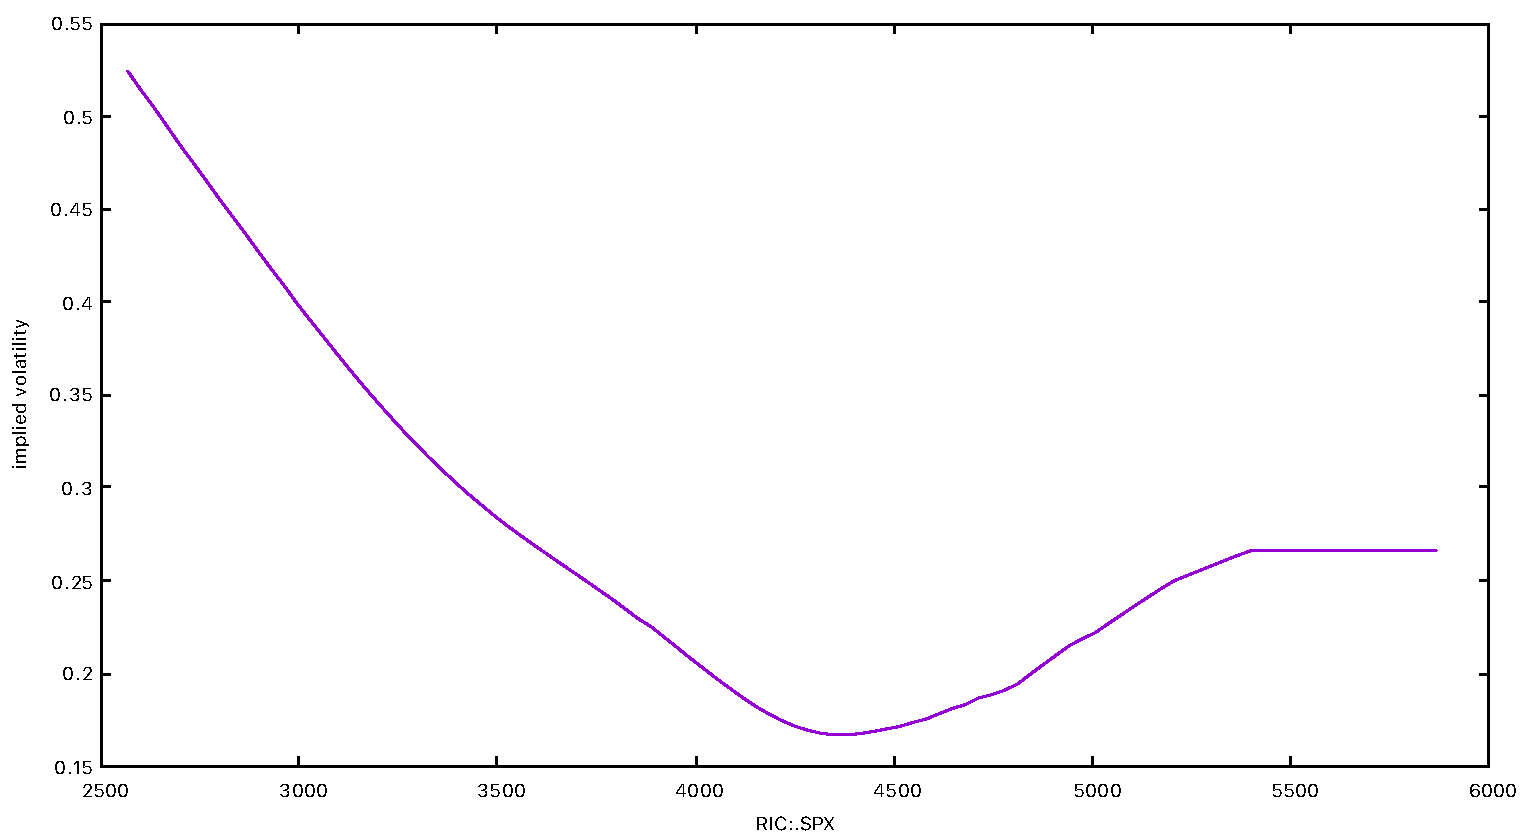
\includegraphics[scale=0.6]{pricing/eq_varianceswap_fig1.pdf}
\end{center}
\caption{Implied volatility of RIC:.SPX at swap maturity $T=0.134247$}
\label{eq_var_swap_fig1}
\end{figure}

\begin{figure}[ht]
\begin{center}
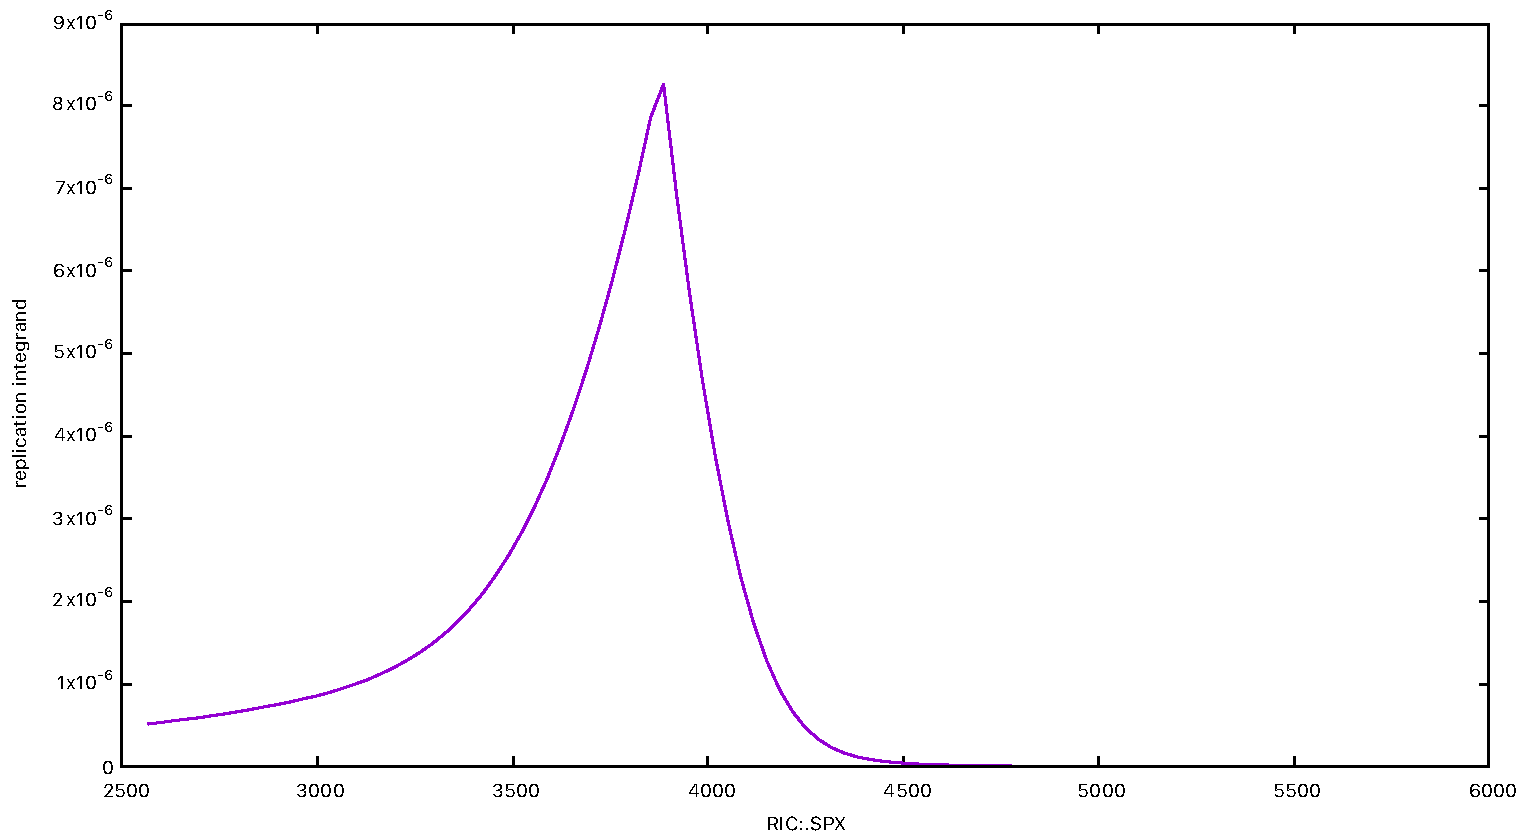
\includegraphics[scale=0.6]{pricing/eq_varianceswap_fig2.pdf}
\end{center}
\caption{The replication integrand, which is given by $\frac{P(K)}{K^2}$ for $K < F$ and $\frac{C(K)}{K^2}$ for $K > F$}
\label{eq_var_swap_fig2}
\end{figure}

\bigskip

\underline{\emph{Total variance:}} The total variance $Var$ in \ref{eq_varianceswap_payoff} is computed as a weighted sum
of the accrued and future variance

$$
Var = \frac{n_1}{n} \text{accrued var} + \frac{n_2}{n} \text{future var}
$$

where

\begin{itemize}
\item $n_1$ is the number of business days between the swap start date and today (both included)
\item $n_2$ is the number of business days between today (excluded) and swap maturity (included)
\item $n$ is the number of business days between the swap start and maturity date (both included)
\end{itemize}

The total variance is available in the additional results under ``totalVariance''. In our case we get

$$
Var = \frac{9}{43}\cdot 0.035178 + \frac{34}{43} 0.062806  = 0.057023
$$

\bigskip

\underline{\emph{Swap NPV:}} The NPV of the swap is finally computed by 

$$
P(0,T) \cdot \omega \cdot N_{var} \cdot 10000 \cdot ( Var - K_{var}  )
$$

with

\begin{itemize}
\item P(0,T) the relevat discount factor for maturity $T$, available in the additional results under ``MaturityDiscountFactor'', in our case $0.993666$
\item the long / short indicator $\omega$ which is $1$ in our case
\item the variance notional $156.25$, available in the additional results under ``VarianceNotional'' (see above for the calculation)
\item the variance strike $0.1024$, available in the additional results under ``VarianceStrike'' (see above for the calculation)
\end{itemize}

This gives a total swap npv of $-70,452.47$ USD.

\bigskip

\underline{\emph{Sensitivity calculation:}} Sensitivities for a variance swap are calculated following a ``bump and
revalue'' approach using the usual configured shift scenarios. The main sensitivities for a variance swap are the
sensitivities to implied volatility (vega) and equity spot price shifts (delta).

There are two major factors impacting the sensitivity to the equity spot:

\begin{itemize}
\item Choice of smile dynamics: ``Sticky Strike'' and ``Sticky Moneyness'' yield different sensitivities to the equity
  spot. The latter choice makes the future variance insensitive to the spot shift, as can be seen from
  \ref{eq_varianceswap_replication}. The former will generate a significant sensitivity to the equity spot on the other
  hand. Both effects are intuitively clear as well.
\item Inlcusion or Exclusion of today's shift contribution (configurable via pricing engine config
  ``StaticTodaysSpot'').
\end{itemize}

Table \ref{eq_var_swap_pricing_sensi_overview} illustrates this by summarizing the sensitivities of our example
trade. Delta is computed w.r.t. a $1\%$ relative shift of the equity spot price, vega w.r.t. to an absolute shift of
$0.01$ in the implied vol and rho w.r.t. a shift of $1$ basispoint on interest rate curves.

\begin{table}[ht]
\begin{center}
\begin{tabular}{l|l|r|r|r}
Smile Dynamics & Todays Shift & Delta & Vega & Rho \\
\hline
Sticky Strike & Included &  -3,622   & 7,357  & -5 \\
Sticky Strike & Excluded &  -4,328   & 7,357  & -5 \\
Sticky Moneyness & Included &  706   & 7,357  & 1 \\
Sticky Moneyness & Excluded &  0 & 7,357  & 1 \\
\end{tabular}
\end{center}
\caption{Variance Swap Sensitivities under different smile dynamics and inclusion / exclusion of today's shift
  contribution}
\label{eq_var_swap_pricing_sensi_overview}
\end{table}

\subsubsection{Equity Position}

The price of an equity position is directly derived from the market quote(s) of the underlying share(s). For a basket
the weighting is taken into account and if equities in several currencies are present in the basket, the equity prices
are converted to a common npv currency using the current FX Spot rates. The npv currency is by convention the currency
of the first equity in the basket.

\subsubsection{Equity Option Position}

The price of an equity option position is derived from the prices of the underlying options, see \ref{pricing:eq_option}
for details on how this is done. For a basket the weighting is taken into account and if equities in several currencies
are present in the basket, the equity prices are converted to a common npv currency using the current FX Spot rates. The
npv currency is by convention the currency of the first equity option in the basket.

\subsubsection{Equity Outperformance Option}
\label{pricing:eq_outperformaceoption}

Equity Outperformace Options are priced analytically using formulas generalized from \cite{Brigo_Mercurio_2006}, 13.16.2.

%- - - - - - - - - - - - - - - - - - - - - - - - - - - - - - - - - - - - - - - - - - - - - - - - - - - - - 
\subsection{FX / Equity / Commodity / Rates / Inflation Exotics}
\subsubsection{Double Digital Option}
\label{pricing::doubledigitaloption}

The double digital option is priced using correlated Black-Scholes processes for the two underlyings. Each process is
calibrated to its quoted market ATM volatility. The correlation is an externally given parameter. The valuation is done
using a Monte Carlo simulation.

See \ref{pricing::scriptedtrade_mc} for more details, the relevant product classification is MultiAssetOption.

\subsubsection{Vanilla European Option Contingent on a Barrier}
\label{pricing::europeanoptionbarrier}

A European option with a barrier in another underlying is priced using correlated Black-Scholes processes for the two underlyings
(option underlying and barrier underlying), unless the option underlying is an IR asset class, in which case we use Gaussian-Cam
for the IR underlying. Each process is calibrated to its quoted market ATM volatility. The correlation is an externally given parameter.
The valuation is done using a Monte Carlo simulation.

See \ref{pricing::scriptedtrade_mc} for more details, the relevant product classification is MultiAssetOption if both underlyings
are Equity, FX or COMM. If the option underlying is IR, then the product classification is IrHybrid.
\subsubsection{Autocallable Type 01}

\ifdefined\IncludePayoff{{\bf Payoff}

The autocallable option of type 01 is characterized by the following data

\begin{itemize}
\item a notional amount $N$
\item a determination level $D$
\item a trigger level $T$
\item The referecne underlying $U$
\item a number of fixing dates $f_i$ for $i=1,\ldots,n$
\item a number of settlement dates $s_i$ for $i=1,\ldots,n$
\item a list of accumulation factors $a_i$ for $i=1,\ldots,n$
\item a cap $C$
\end{itemize}

On each fixing date $f_i$ for $i=1,\ldots,n$, if the underlying spot is at or below the trigger level, i.e.

$$U(f_i) <= T$$

the option holder receives an amount

$$N\cdot a_i$$

on the settlement date $s_i$ and the structure terminates on this same date.

If no trigger event occurs on any of the fixing dates and if the underlying spot is above the determination level on the
{\em last} fixing date $f_n$, i.e.

$$U(f_n) > D$$

then the option holder {\em pays} an amount

$$N \min(C, (U(f_n) - D))$$

to the counterparty of the transaction. The underlying can be an Equity, FX or Commodity underlying.

{\bf Input}}\fi

The \verb+Autocallable_01+ node is the trade data container for the Autocallable\_01 trade type, listing
\ref{lst:autocallable01_data} shows the structure of an example.

\begin{listing}[H]
\begin{minted}[fontsize=\footnotesize]{xml}
    <Autocallable01Data>
      <NotionalAmount>12000000</NotionalAmount>
      <DeterminationLevel>11.0</DeterminationLevel>
      <TriggerLevel>9.8</TriggerLevel>
      <Underlying>
        <Type>FX</Type>
        <Name>ECB-EUR-NOK</Name>
      </Underlying>
      <Position>Long</Position>
      <PayCcy>EUR</PayCcy>
      <FixingDates>
        <ScheduleData>
          <Dates>
            <Dates>
              <Date>2018-09-27</Date>
              <Date>2019-09-27</Date>
              <Date>2020-09-27</Date>
              <Date>2021-09-29</Date>
              <Date>2022-09-28</Date>
            </Dates>
          </Dates>
        </ScheduleData>
      </FixingDates>
      <SettlementDates>
        <ScheduleData>
          <Dates>
            <Dates>
              <Date>2018-10-07</Date>
              <Date>2019-10-09</Date>
              <Date>2020-10-07</Date>
              <Date>2021-10-07</Date>
              <Date>2022-10-07</Date>
            </Dates>
          </Dates>
        </ScheduleData>
      </SettlementDates>
      <AccumulationFactors>
        <Factor>0.344</Factor>
        <Factor>0.733</Factor>
        <Factor>0.911</Factor>
        <Factor>1.123</Factor>
        <Factor>1.544</Factor>
      </AccumulationFactors>
      <Cap>1.0</Cap>
    </Autocallable01Data>
\end{minted}
\caption{Autocallable Type 01 data}
\label{lst:autocallable01_data}
\end{listing}

If a trigger event occurs on the $i$-th fixing date, the option holder receives the following:

\begin{equation*}
  Payout = \text{\lstinline!NotionalAmount!} * AccumulationFactor_i.
\end{equation*}

If a trigger event never occurs and the underlying spot at the fixing date $f_n$ is above the \lstinline!DeterminationLevel!,
the option holder pays the following:

\begin{equation*}
  Payout = \min (\text{\lstinline!Cap!}, \text{\lstinline!Underlying!}(f_n) - \text{\lstinline!DeterminationLevel!}).
\end{equation*}

The meanings and allowable values of the elements in the \verb+Autocallable01Data+ node follow below.

\begin{itemize}
\item NotionalAmount: The notional amount of the option. Allowable values are non-negative numbers.
\item DeterminationLevel: The determination level. For an FX underlying FX-SOURCE-CCY1-CCY2 this is the number of units
  of CCY2 per units of CCY1. For an EQ underlying this is the equity price expressed in the equity ccy.  Allowable
  values are non-negative numbers.
\item TriggerLevel: The trigger level. For an FX underlying FX-SOURCE-CCY1-CCY2 this is the number of units of CCY2 per
  units of CCY1. For an EQ underlying this is the equity price expressed in the equity ccy.  Allowable values are
  non-negative numbers.
\item Underlying: The option underlying, see \ref{ss:underlying}.
\item Position: The option position type. Allowable values: {\em Long} or {\em Short}.
\item PayCcy: The pay currency of the option. See the appendix for allowable currency codes.
\item FixingDates: The fixing date schedule given as a \verb+ScheduleData+ subnode, see \ref{ss:schedule_data}
\item SettlementDates: The settlement date schedule given as a \verb+ScheduleData+ subnode, see \ref{ss:schedule_data}
\item AccumulationFactors: The accumulation factors given as a list of values corresponding to the fixing
  dates. Allowable values are non-negative numbers.
\item Cap: The maximum amount, per unit of notional, payable by the option holder if a trigger event never occurred
(i.e.\ underlying value was never below the \verb+TriggerLevel+ on any of the fixing dates) and if the underlying value
is greater than the \verb+DeterminationLevel+ at the last fixing date. Allowable values are non-negative numbers.
\end{itemize}

\subsubsection{Performance Option Type 01}

The performace option of type ``01'' is characterized by the following data

\begin{itemize}
\item a notional amount $N$
\item a participation rate $q$
\item a valuation date $V$ and a settlement date $S$
\item a number of underlyings $U_i$ for $i=1,\ldots,n$
\item weights for the underlyings $w_i$ for $i=1,\ldots,n$
\item initial strike prices for the underlyings $s_i$ for $i=1,\ldots,n$
\item an option strike $K$
\end{itemize}

On the valuation date the average performance of the underlying basket is computed as

$$
P = \max\left( \sum_{i=1}^n w_i \left( \frac{U_i(V)}{s_i} - K \right), 0 \right)
$$

The option holder receives an amount $N\cdot q\cdot P$ on the settlement date $S$. The underlyings can be Equity, FX or
Commodity underlyings.

The above payoff includes the strike in the performance calculation. There is another variant with excluded strike and payoff:

$$
P = \max\left( \left[ \sum_{i=1}^n w_i \frac{U_i(V)}{s_i} \right] - K, 0 \right)
$$

The \verb+PerformanceOption_01+ node is the trade data container for the PerformanceOption\_01 trade type, listing
\ref{lst:performanceoption01_data} shows the structure of an example.

\begin{listing}[H]
\begin{minted}[fontsize=\footnotesize]{xml}
    <PerformanceOption01Data>
      <NotionalAmount>12500000</NotionalAmount>
      <ParticipationRate>0.9</ParticipationRate>
      <ValuationDate>2022-05-03</ValuationDate>
      <SettlementDate>2022-05-05</SettlementDate>
      <Underlyings>
        <Underlying>
          <Type>FX</Type>
          <Name>ECB-CHF-EUR</Name>
          <Weight>0.34</Weight>
        </Underlying>
        <Underlying>
          <Type>FX</Type>
          <Name>ECB-NOK-EUR</Name>
          <Weight>0.32</Weight>
        </Underlying>
        <Underlying>
          <Type>FX</Type>
          <Name>ECB-SEK-EUR</Name>
          <Weight>0.24</Weight>
        </Underlying>
        <Underlying>
          <Type>FX</Type>
          <Name>ECB-SEK-EUR</Name>
          <Weight>0.10</Weight>
        </Underlying>
      </Underlyings>
      <StrikePrices>
        <StrikePrice>0.910002</StrikePrice>
        <StrikePrice>0.097192</StrikePrice>
        <StrikePrice>0.096085</StrikePrice>
        <StrikePrice>0.035032</StrikePrice>
      </StrikePrices>
      <Strike>1.15</Strike>
      <StrikeIncluded>true</StrikeIncluded>
      <Position>Long</Position>
      <PayCcy>EUR</PayCcy>
    </PerformanceOption01Data>
\end{minted}
\caption{Performance Option Type 01 data}
\label{lst:performanceoption01_data}
\end{listing}

The meanings and allowable values of the elements in the \verb+PerformanceOption01Data+  node follow below.

\begin{itemize}
\item NotionalAmount: The notional amount of the option. Allowable valus are non-negative numbers.
\item ParticipationRate: The participation rate. Allowable values are non-negative numbers. Usually the value will be
  between 0 and 1.
\item ValuationDate: The valuation date.  Allowable values are valid dates.
\item SettlementDate: The settlement date. Allowable values are valid dates.
\item Underlyings: The underlyings of the option. See \ref{ss:underlying} for each underlying.
\item StrikePrices: The initial strike prices of the underlyings. For an FX underlying FX-SOURCE-CCY1-CCY2 this is the
  number of units of CCY2 per units of CCY1. For an EQ underlying this is the equity price expressed in the equity ccy. For a Commodity underlying this is the commodity price quoted as per the underlying commodity.
  Allowable values are non-negative numbers.
\item Strike: The option strike. This is expressed in terms of the performance of the underlying basket (see the product
  description for more details). Allowable values are numbers.
\item StrikeIncluded [optional]: If true the strike is included in the performance calculation, this is also the default
  if the flag not given. If false the strike is excluded. 
\item Position: The option position. Allowable values are {\em Long} or {\em Short}.
\item PayCcy: The payment currency of the option. See the appendix for allowable currency codes.
\end{itemize}

\subsubsection{Equity Cliquet Option}
\label{pricing::eq_cliquetoption}

The cliquet option is priced using a Black-Scholes process for the underlying 
which is calibrated to its quoted market ATM volatility. The valuation is 
done using a Monte Carlo simulation.

\subsubsection{Window Barrier Option}
\label{pricing:window_barrieroption}

EQ/FX/COMM window barrier options are priced using a Black-Scholes process for the underlying calibrated to the option
strike. The valuation is done using a Monte Carlo simulation.

See \ref{pricing::scriptedtrade_mc} for more details, the relevant product classification is SingleAssetOption.

\subsubsection{Generic Barrier Option}
\label{pricing:generic_barrieroption}
Generic Barrier Options are priced using a finite-difference solver in a Black-Scholes model. The final payoff $V(T,S(T))$
at the option expiry $T$ dependent on the underlying value $S(T)$ is easily generated, including an additional
transatlantic barrier condition. We use the notation as in table \ref{tab:generic_barrier_pricing_notation}

\begin{table}[h]
  \begin{tabular}{p{3cm}|p{11cm}}
    Variable & Meaning \\ \hline
    $V_{V}(t,S)$ & Value of the option conditional on $(t,S)$, this excludes rebate payments and assumes barrier monitoring from $t$ on\\ \hline
    $V_{NA}(t,S)$ & Value of the final payoff at $t$ conditional on no knock events happening for times $s$ with $s \geq t$ \\ \hline
    $V_{KI}(t,S)$ & Value of the final payoff at $t$ conditional on a KI event but no KO event happening for a time $s$ with $s \geq t$ \\ \hline
    $V_{KO}(t,S)$ & Value of the final payoff at $t$ conditional on a KO event but no KI event happening for a time $s$ with $s \geq t$ \\ \hline
    $V_{KIKO}(t,S)$ & Value of the final payoff at $t$ conditional on a KI event at time $u$ and a KO event at $v$ with $t\leq u<v$) \\ \hline
    $V_{KOKI}(t,S)$ & Value of the final payoff at $t$ conditional on a KO event at time $u$ and a KI event at $v$ with $t\leq u<v$) \\ \hline
  \end{tabular}
  \caption{Values in FD backward solver}
  \label{tab:generic_barrier_pricing_notation}
\end{table}

The idea is that we track future Knock events. For a series of future knock events we collapse neighboring events of the
same type ``in'' and ``out'' into a single event (because only the first is relevant). Also we only look two events into
the future, since this is sufficient for the update rules below. Notice that for this purpose we ignore whether the
events as allowed in this order according to the term sheet, i.e. we track a sequence of KI then KO events in $V_{KIKO}$
even if KoBeforeKi is defined, i.e. the KO event is excluded by the termsheet in this case. Also notice, that $V_{x}$
for $x \in \{ NA, KI, KO, KIKO, KOKI \}$ is the value of the final payoff, i.e. without considering KI or KO events in
the value itself. This is different for $V_{V}$, where we account for exluded barrier events and include the barrier
events in the value.

At expiry we set $V_{V} = V$ if no KI barrier is defined and $V_{V} = 0$ if a KI barrier is defined. Furthermore we set
$V_{NA} = V$ and $V_x = 0$ for $x \in \{ KI, KO, KIKO, KOKI \}$. The rollback from $t_{i+1}$ to $t_i$ works as follows:

If there is no KI or KO event at $t_i$, all values are rolled back without any update.

If there is a KI event at $t_i$, we apply the following updates after the roll back:

\begin{itemize}
\item $V_{KIKO} := V_{KO} + V_{KIKO} + V_{KOKI}$
\item $V_{KOKI} := 0$
\item $V_{KI} := V_{NA} + V_{KI}$
\item $V_{KO} := 0$
\item $V_{NA} := 0$
\item $V_{V} := V_{KI}$, add $V_{KIKO}$ if KoBeforeKi
\end{itemize}

If there is a KO event at $t_i$, we apply the following updates after the roll back:

\begin{itemize}
\item $V_{KOKI} := V_{KI} + V_{KOKI} + V_{KIKO}$
\item $V_{KIKO} := 0$
\item $V_{KO} := V_{NA} + V_{KO}$
\item $V_{KI} := 0$
\item $V_{NA} := 0$
\item $V_{V} := 0$ if KoAlways or KoBeforeKi
\end{itemize}

If the trade is seasoned we continue the rollback into the past to account for past KI and KO events properly. This
rollback does not involve the computation of conditional expectations though, we only update the values according to the
rules above.

Rebates are handled as follows:

The Transatlantic Barrier Rebate is incorporated into the final option payoff, i.e. for
the nodes where the Transatlantic Barrier deactivates the option, a payoff amount equal to the rebate amount is
generated.

If only KO-Barriers are present, the rebate NPV is computed in the PDE by setting $V_{V}$ to the rebate amount (instead
of $0$) on nodes where a KO event is detected. The payment timing is accounted for by appropriate discounting of that
amount.

If at least one KI-Barrier barrier is present, only a unique rebate amount is allowed which is always paid on the option
settlement date. We can roll back this amount as $R_x$ in complete analogy to the $V_x$ for $x \in \{ NA, KI, KO, KIKO,
KOKI \}$. The variables $R_x$ are initialised in the same way as $V_x$, but with the final option payoff replaced with
the rebate payment $R$. The rebate NPV is then computed as the discounted value of $R$ at $t=0$ minus $R_V$ (because
$R_V$ represents an option that pays $R$ at maturity if the original barrier option is active).

When evaluated via Monte-Carlo simulation, the exercise probability and the trigger probability are 
given as additional results. Additional to this, the knock-out probability of the transatlantic feature is given as well if relevant. 
Therein, there are the following definitions active:

\begin{table}[h]
  \begin{tabular}{p{4.5cm}|p{8cm}}
      Additional Result&Description\\ 
      \hline
      ExerciseProbability&The estimated probability of the exercise event. The latter means that the payoff 
      is non-zero at maturity (i.e. the plain vanilla part of the payoff is positive and no knock-out event 
      has accured and necessary knock-in events have occured until then).\\ \hline
      TriggerProbability&The estimated probability of the exercise event. The latter means that the knock-in 
      or the knock-out event (or one of them if there are multiple ones) has been triggered.\\ \hline      
      TransatlanticTriggered&The estimated probability of the transatlantic trigger event. The latter means 
      that the transatlantic knock-out event (or at least one of them if there are multiple ones) has been triggerd.\\ \hline
  \end{tabular}
  \caption{Additional results output labels for the Generic Barrier Option}
  \label{tab:AdditionalResultsGenericBarrier}
\end{table}



\subsubsection{Best Entry Option}
\label{input:bestentryoption}

\ifdefined\IncludePayoff{{\bf Payoff}

The Best Entry Option is an option on a single underlying that has a payoff contingent on the `best entry' of the underlying index into a specified region on a set of specified `strike observation dates', which is determined by a single barrier.

On the option expiry date, if the value of the underlying index (denoted `$Index_{Final}$') is greater than or equal to the strike price $K$, the payoff of the option is given by:
\begin{align*}
	\text{Notional} \times \text{Multiplier} \times \text{min}\left(\text{Cap}, \text{max}\left(0, \frac{Index_{Final} - Index_{Initial}}{Index_{Inital}}\right)\right).
\end{align*}
If $Index_{Final}$ is less than $K$, the payoff is given by
\begin{align*}
	-\text{Notional} \times \frac{K - Index_{Final}}{Index_{Initial}}.
\end{align*}
Here, $Index_{Initial}$ is defined as
\begin{itemize}
	\item{The level of the underlying index on a pre-determined `strike date', if the level of the index on any of the strike observation dates is \emph{not} lower than the barrier level,}
	\item{The maximum between the `reset minimum value' and the lowest index level on a strike observation date, if the level of the index does indeed hit the barrier level at least once.}
\end{itemize}

{\bf Input}}\fi

Best Entry Options are defined using one of the trade types \emph{FxBestEntryOption}, \emph{EquityBestEntryOption},
\emph{CommodityBestEntryOption} depending on the underlying asset class and an associated node FxBestEntryOptionData,
EquityBestEntryOptionData, CommodityBestEntryOptionData. Listing \ref{lst:bestentryoption_data} shows an
example for an Equity Underlying. For a more detailed description of the computation of the payoff of this option, please see the product description. The nodes have the following meaning:

\begin{itemize}
\item Underlying: The underlying definition. Note that for FX underlyings the order of the currencies defines the
  observed underlying value, i.e. for EUR-USD the domestic currency is USD (the observed value is e.g. $1.2$ USD per
  EUR) while for USD-EUR the domestic currency is EUR (the observed value is e.g. $0.8$ EUR per USD).

  Allowable Values: See \ref{ss:underlying}

\item Currency: The payment currency.

  Allowable Values: See \lstinline!Currency!  in Table \ref{tab:allow_stand_data}.

\item SettlementDate: The date on which the option payoff is settled. The SettlementDate is used unadjusted
  as given. 

  Allowable Values: any valid date greater or equal to the exercise date.

\item Notional: The notional amount. 

  Allowable Values: any real number

\item Strike: The strike value used to compute the payoff of the option. This value should be provided as a decimal, representing a percentage of the value of $Index_{Initial}$, e.g. a value of $K = 0.6 \implies 0.6 \times Index_{Initial}$ in the computation of the payoff. 
  Allowable Values: any real number

\item Multiplier: The payoff multiplier used in the case that the underlying index is greater than the strike on the settlement date. If omitted defaults to $1$.

  Allowable Values: any real number

\item TriggerLevel: The value that is compared to the underlying index on each strike observation date to determine if a Trigger Event has occurred. This should be provided as a decimal, representing a percentage of the value of Strike Index Level, ie the value of the underlying on the \lstinline!StrikeDate!.

  Allowable Values: any real number

\item LongShort: Denotes whether the payoff is computed relative to the holder or seller of the option.  

  Allowable Values: \emph{Long}, \emph{Short}.

\item Cap: The maximum value of the payoff (before the notional and multiplier are applied). This value should be interpreted as a percentage and should be in decimal format in the trade XML, e.g. $0.06 = 6\%$.

  Allowable Values: any real number

\item ResetMinimum: The minimum value of $Index_{Initial}$ in the case that a Trigger Event has occurred at least once during the option's lifetime. This should be provided as a decimal, representing a percentage of the value of Strike Index Level used in the computation of $Index_{Initial}$.

  Allowable Value: any real number

\item StrikeDate: The date on which the level on the underlying index is used to compute the payoff, in the case that there has not been a Trigger Event during the option's lifetime.

  Allowable Value: any valid date before the option expiry date.

\item ExpiryDate: The date on which the option expires and the payoff is computed.

  Allowable Values: any valid date before the SettlementDate

\item Premium: The option premium. Defaults to $0$.

  Allowable Values: any real number.

\item PremiumDate: The date on which the option premium is paid.

  Allowable Values: any valid date.

\item StrikeObservationDates: The set of dates on which the underlying index level is observed - the lowest of which is used to compute the option payoff if the underlying index is greater than the strike on the expiry date.

  Allowable Values: any valid dates schedule (see \ref{ss:schedule_data}).




\end{itemize}

\begin{listing}[H]
\begin{minted}[fontsize=\footnotesize]{xml}
    <EquityBestEntryOptionData>
      <LongShort>Long</LongShort>
      <Strike>0.85</Strike>
      <Cap>0.06</Cap>
      <ResetMinimum>0.85</ResetMinimum>
      <Notional>1000000</Notional>
      <Multiplier>1</Multiplier>
      <TriggerLevel>0.95</TriggerLevel>
      <SettlementDate>2021-11-20</SettlementDate>
      <PremiumDate>2021-11-22</PremiumDate>
      <StrikeDate>2020-12-15</StrikeDate>
      <Underlying>
        <Type>Equity</Type>
        <Name>RIC:.SPX</Name>
      </Underlying>
      <StrikeObservationDates>
        <Dates>
          <Dates>
            <Date>2021-03-01</Date>
            <Date>2021-06-01</Date>
            <Date>2021-09-01</Date>
          </Dates>
        </Dates>
      </StrikeObservationDates>
      <Currency>USD</Currency>
      <Premium>100</Premium>
      <ExpiryDate>2021-11-20</ExpiryDate>
    </EquityBestEntryOptionData>
\end{minted}
\caption{Best Entry Option data (Equity Underlying)}
\label{lst:bestentryoption_data}
\end{listing}

\subsubsection{Basket Options}

Basket Options are represented as traditional trades or {\em scripted trades}, refer to ore/Docs/ScriptedTrade
for an introduction of the latter. Each of the supported variations is represented by a separate payoff script as shown
in Table \ref{tab:basketoptions}.

\begin{table}[hbt]
\begin{center}
\begin{tabular}{|l|l|}
\hline
Basket Option Type & Payoff Script Name \\
\hline
\hline
Vanilla & VanillaBasketOption \\
\hline
Asian & AsianBasketOption \\
\hline
Average strike & AverageStrikeBasketOption \\
\hline
Lookback call & LookbackCallBasketOption \\
\hline
Lookback put & LookbackPutBasketOption \\
\hline
\end{tabular}
\end{center}
\caption{Basket option types and associated script names.}
\label{tab:basketoptions}
\end{table}

The supported underlying types are Equity, Fx or Commodity resulting in corresponding trade types and trade data
container names

\begin{itemize}
  \item EquityBasketOption / EquityBasketOptionData
  \item FxBasketOption / FxBasketOptionData
  \item CommodityBasketOption / CommodityBasketOptionData
\end{itemize}

Trade input and the associated payoff script are described in the following for all supported Basket Option variations.

\subsubsection*{Vanilla Basket Option}

The traditional trade representation is as follows, using an equity underlying in this example:

\begin{minted}[fontsize=\scriptsize]{xml}
<Trade id="VanillaBasketOption#1">
  <TradeType>EquityBasketOption</TradeType>
  <Envelope>
    <CounterParty>CPTY_A</CounterParty>
    <NettingSetId>CPTY_A</NettingSetId>
    <AdditionalFields/>
  </Envelope>
  <EquityBasketOptionData>
    <Currency>USD</Currency>
    <Notional>1</Notional>
    <Strike>5000</Strike>
    <Underlyings>
      <Underlying>
        <Type>Equity</Type>
        <Name>RIC:.SPX</Name>
        <Weight>1.0</Weight>
      </Underlying>
      <Underlying>
        <Type>Equity</Type>
        <Name>RIC:.STOXX50E</Name>
        <Currency>EUR</Currency>
        <Weight>1.0</Weight>
      </Underlying>
    </Underlyings>
    <OptionData>
      <LongShort>Long</LongShort>
      <OptionType>Call</OptionType>
      <PayoffType>Vanilla</PayoffType>
      <ExerciseDates>
        <ExerciseDate>2020-02-15</ExerciseDate>
      </ExerciseDates>
      <Premiums> ... </Premiums>
    </OptionData>
    <Settlement>2020-02-20</Settlement>
  </EquityBasketOptionData>
</Trade>
\end{minted}

with the following elements:

\begin{itemize}
\item Currency: The pay currency. Notice section ``Payment Currency'' in ore/Docs/ScriptedTrade. \\
  Allowable values: all supported currency codes, see Table \ref{tab:currency} \lstinline!Currency!.
\item Notional: The quantity (for equity, commodity underlyings) / foreign amount (fx underlying) \\
  Allowable values: all positive real numbers
\item Strike: The strike of the option \\
  Allowable values: all positive real numbers
\item Underlyings: The basket of underlyings. \\
  Allowable values: for each underlying see \ref{ss:underlying}
\item OptionData: relevant are the long/short flag, the call/put flag, the payoff type (must be set to Vanilla to
  identify the payoff), and the exercise date (exactly one date must be given). A \emph{Premiums} node can be added to represent deterministic option premia to be paid by the option holder. \\
  Allowable values: see \ref{ss:option_data} for the general structure of the option data node
\item Settlement: the settlement date (optional, if not given defaults to the exercise date) \\
  Allowable values: each valid date.
\end{itemize}

The representation as a scripted trade is as follows:

\begin{minted}[fontsize=\scriptsize]{xml}
<Trade id="VanillaBasketOption#1">
  <TradeType>ScriptedTrade</TradeType>
  <Envelope/>
  <VanillaBasketOptionData>
    <Expiry type="event">2020-02-15</Expiry>
    <Settlement type="event">2020-02-20</Settlement>
    <PutCall type="optionType">Call</PutCall>
    <LongShort type="longShort">Long</LongShort>
    <Notional type="number">1</Notional>
    <Strike type="number">5000</Strike>
    <Underlyings type="index">
      <Value>EQ-RIC:.SPX</Value>
      <Value>EQ-RIC:.STOXX50E</Value>
    </Underlyings>
    <Weights type="number">
      <Value>1.0</Value>
      <Value>1.0</Value>
    </Weights>
    <PayCcy type = "currency">USD</PayCcy>
  </VanillaBasketOptionData>
</Trade>
\end{minted}

The VanillaBasketOption script referenced in the trade above is
shown in Listing \ref{lst:vanillabasketoption}.

\begin{listing}[hbt]
\begin{minted}[fontsize=\scriptsize]{Basic}
REQUIRE SIZE(Underlyings) == SIZE(Weights);

NUMBER u, basketPrice, ExerciseProbability, Payoff, currentNotional;

FOR u IN (1, SIZE(Underlyings)) DO
    basketPrice = basketPrice + Underlyings[u](Expiry) * Weights[u];
END;

Payoff = max(PutCall * (basketPrice - Strike), 0);

Option = LongShort * Notional * PAY(Payoff, Expiry, Settlement, PayCcy);

IF Payoff > 0 THEN
    ExerciseProbability = 1;
END;
currentNotional = Notional * Strike;
\end{minted}
\caption{Payoff script for a VanillaBasketOption.}
\label{lst:vanillabasketoption}
\end{listing}

The meanings and allowable values of the elements in the
\lstinline!VanillaBasketOptionData! node are given below, with data
type indicated in square brackets.

\begin{itemize}
    \item{}[event] \lstinline!Expiry!: Option expiry date. \\
    Allowable values: See \lstinline!Date! in Table \ref{tab:allow_stand_data}.
    \item{}[event] \lstinline!Settlement!: Option settlement date. \\
    Allowable values: See \lstinline!Date! in Table \ref{tab:allow_stand_data}.
    \item{}[optionType] \lstinline!PutCall!: Option type with \\
          Allowable values \emph{Call, Put}.
    \item{}[longShort] \lstinline!LongShort!: Position type,
          {\em Long} if we buy, {\em Short} if we sell.\\
    Allowable values: \emph{Long, Short}.
     \item{}[number] \lstinline!Notional!: Quantity multiplier applied to the basket price \\
          Allowable values: Any positive real number.
     \item{}[number] \lstinline!Strike!: Strike basket price in PayCcy (see below) \\
          Allowable values: Any positive real number.
     \item{}[index] \lstinline!Underlyings!:
          List of underlying indices enclosed by {\tt <Value>} and {\tt </Value>} tags. \\
          Allowable values: See ore/Docs/ScriptedTrade's Index Section for allowable values.
    \item{}[number] \lstinline!Weights!: List of weights applied to the
      underlying prices in the basket, given in the same order as
      the Underlyings above, each weight enclosed by {\tt <Value>} and {\tt </Value>} tags.\\
      Allowable values: Any positive real number.
    \item{}[currency] \lstinline!PayCcy!: The payment currency. For FX, where the underlying is provided
    in the form \lstinline!FX-SOURCE-CCY1-CCY2! (see Table \ref{tab:fxindex_data}) this should
    be \lstinline!CCY2!. If \lstinline!CCY1! or the currency of the underlying (for EQ and
    COMM underlyings), this will result in a quanto payoff. Notice section ``Payment Currency'' in ore/Docs/ScriptedTrade.
      Allowable values: See Table \ref{tab:currency} \lstinline!Currency!
      for allowable currency codes.
\end{itemize}

\subsubsection*{Asian Basket Option}

The traditional trade representation is as follows, using an equity underlying in this example:

\begin{minted}[fontsize=\scriptsize]{xml}
<Trade id="AsianBasketOption#1">
  <TradeType>EquityBasketOption</TradeType>
  <Envelope>
    <CounterParty>CPTY_A</CounterParty>
    <NettingSetId>CPTY_A</NettingSetId>
    <AdditionalFields/>
  </Envelope>
  <EquityBasketOptionData>
    <Currency>USD</Currency>
    <Notional>1</Notional>
    <Strike>5000</Strike>
    <Underlyings>
      <Underlying>
        <Type>Equity</Type>
        <Name>RIC:.SPX</Name>
        <Currency>USD</Currency>
        <Weight>1.0</Weight>
      </Underlying>
      <Underlying>
        <Type>Equity</Type>
        <Name>RIC:.STOXX50E</Name>
        <Weight>1.0</Weight>
      </Underlying>
    </Underlyings>
    <OptionData>
      <LongShort>Long</LongShort>
      <OptionType>Call</OptionType>
      <PayoffType>Asian</PayoffType>
      <ExerciseDates>
        <ExerciseDate>2020-02-15</ExerciseDate>
      </ExerciseDates>
      <Premiums> ... </Premiums>  
    </OptionData>
    <Settlement>2020-02-20</Settlement>
    <ObservationDates>
        <Rules>
          <StartDate>2019-02-06</StartDate>
          <EndDate>2020-02-06</EndDate>
          <Tenor>1D</Tenor>
          <Calendar>US</Calendar>
          <Convention>F</Convention>
          <TermConvention>F</TermConvention>
          <Rule>Forward</Rule>
        </Rules>
    </ObservationDates>
  </EquityBasketOptionData>
</Trade>
\end{minted}

with the following elements:

\begin{itemize}
\item Currency: The pay currency. Notice section ``Payment Currency'' in ore/Docs/ScriptedTrade. \\
  Allowable values: all supported currency codes, see Table \ref{tab:currency} \lstinline!Currency!.
\item Notional: The quantity (for equity, commodity underlyings) / foreign amount (fx underlying) \\
  Allowable values: all positive real numbers
\item Strike: The strike of the option \\
  Allowable values: all positive real numbers
\item Underlyings: The basket of underlyings. \\
  Allowable values: for each underlying see \ref{ss:underlying}
\item OptionData: relevant are the long/short flag, the call/put flag, the payoff type (must be set to Asian to
  identify the payoff), and the exercise date (exactly one date must be given). \lstinline!PayoffType2! can be optionally set to \emph{Arithmetic} or \emph{Geometric} and defaults to \emph{Arithmetic} if not given. Furthermore, a \emph{Premiums} node can be added to represent deterministic option premia to be paid by the option holder. \\
  Allowable values: see \ref{ss:option_data} for the general structure of the option data node
\item Settlement: the settlement date (optional, if not given defaults to the exercise date) \\
  Allowable values: each valid date.
\item ObservationDates: the observation dates for the asian \\
  Allowable values: See the definition in \ref{ss:schedule_data}
\end{itemize}

The representation as a scripted trade is as follows:

\begin{minted}[fontsize=\scriptsize]{xml}
<Trade id="AsianBasketOption#1">
  <TradeType>ScriptedTrade</TradeType>
  <Envelope/>
   <AsianBasketOptionData>
    <Expiry type="event">2020-02-15</Expiry>
    <Settlement type="event">2020-02-20</Settlement>
    <ObservationDates type="event">
      <ScheduleData>
        <Rules>
          <StartDate>2019-02-06</StartDate>
          <EndDate>2020-02-06</EndDate>
          <Tenor>1D</Tenor>
          <Calendar>US</Calendar>
          <Convention>F</Convention>
          <Rule>Forward</Rule>
        </Rules>
      </ScheduleData>
    </ObservationDates>
    <PutCall type="optionType">Call</PutCall>
    <LongShort type="longShort">Long</LongShort>
    <Notional type="number">1</Notional>
    <Strike type="number">5000</Strike>
    <Underlyings type="index">
      <Value>EQ-RIC:.SPX</Value>
      <Value>EQ-RIC:.STOXX50E</Value>
    </Underlyings>
    <Weights type="number">
      <Value>1.0</Value>
      <Value>1.0</Value>
    </Weights>
    <PayCcy type="currency">USD</PayCcy>
  </AsianBasketOptionData>
</Trade>
\end{minted}

The AsianBasketOption script referenced in the trade above is
shown in Listing \ref{lst:asianbasketoption}.

\begin{listing}[hbt]
\begin{minted}[fontsize=\scriptsize]{Basic}
REQUIRE SIZE(Underlyings) == SIZE(Weights);

NUMBER d, u, basketPrice, ExerciseProbability, Payoff;
NUMBER currentNotional;

FOR d IN (1, SIZE(ObservationDates)) DO
    FOR u IN (1, SIZE(Underlyings)) DO
        basketPrice = basketPrice + Underlyings[u](ObservationDates[d]) * Weights[u];
    END;
END;

basketPrice = basketPrice / SIZE(ObservationDates);

Payoff = max(PutCall * (basketPrice - Strike), 0);

Option = LongShort * Notional * PAY(Payoff, Expiry, Settlement, PayCcy);

IF Payoff > 0 THEN
    ExerciseProbability = 1;
END;

currentNotional = Notional * Strike;
\end{minted}
\caption{Payoff script for an AsianBasketOption.}
\label{lst:asianbasketoption}
\end{listing}

The meanings and allowable values of the elements in the
\lstinline!AsianBasketOptionData! node are given below, with data
type indicated in square brackets.

\begin{itemize}
    \item{}[event] \lstinline!Expiry!: Option expiry date. \\
    Allowable values: See \lstinline!Date! in Table \ref{tab:allow_stand_data}.
    \item{}[event] \lstinline!Settlement!: Option settlement date. \\
    Allowable values: See \lstinline!Date! in Table \ref{tab:allow_stand_data}.
    \item{}[event] \lstinline!ObservationDates!: Price monitoring schedule. \\
    Allowable values: See section \ref{ss:schedule_data} Schedule Data and Dates, or DerivedSchedule (see ore/Docs/ScriptedTrade).
    \item{}[optionType] \lstinline!PutCall!: Option type with \\
          Allowable values \emph{Call, Put}.
    \item{}[longShort] \lstinline!LongShort!: Position type,
          {\em Long} if we buy, {\em Short} if we sell.\\
    Allowable values: \emph{Long, Short}.
        \item{}[number] \lstinline!Notional!: Quantity multiplier applied to the
          basket price \\
          Allowable values: Any positive real number.
        \item{}[number] \lstinline!Strike!: Strike basket price in PayCcy (see
          below) \\
          Allowable values: Any positive real number.
    \item{}[index] \lstinline!Underlyings!: List of underlying indices
      enclosed by {\tt <Value>} and {\tt </Value>} tags. \\
      See ore/Docs/ScriptedTrade's Index Section for allowable values.
    \item{}[number] \lstinline!Weights!: List of weights applied to the
          underlying prices in the basket, given in the same order as
          the Underlyings above, each weight enclosed by {\tt <Value>} and {\tt </Value>} tags.\\
          Allowable values: Any positive real number.
    \item{}[currency] \lstinline!PayCcy!: The payment currency. For FX, where the underlying is provided
      in the form \lstinline!FX-SOURCE-CCY1-CCY2! (see Table \ref{tab:fxindex_data}) this should
      be \lstinline!CCY2!. If \lstinline!CCY1! or the currency of the underlying (for EQ and
      COMM underlyings), this will result in a quanto payoff. Notice section ``Payment Currency'' in ore/Docs/ScriptedTrade. \\
        Allowable values: See Table \ref{tab:currency} \lstinline!Currency! for allowable currency codes.
\end{itemize}

\subsubsection*{Average Strike Basket Option}

The traditional trade representation is as follows, using an equity underlying in this example:

\begin{minted}[fontsize=\scriptsize]{xml}
<Trade id="AverageStrikeBasketOption#1">
  <TradeType>EquityBasketOption</TradeType>
  <Envelope>
    <CounterParty>CPTY_A</CounterParty>
    <NettingSetId>CPTY_A</NettingSetId>
    <AdditionalFields/>
  </Envelope>
  <EquityBasketOptionData>
    <Currency>USD</Currency>
    <Notional>1</Notional>
    <Underlyings>
      <Underlying>
        <Type>Equity</Type>
        <Name>RIC:.SPX</Name>
        <Currency>USD</Currency>
        <Weight>1.0</Weight>
      </Underlying>
      <Underlying>
        <Type>Equity</Type>
        <Name>RIC:.STOXX50E</Name>
        <Weight>1.0</Weight>
      </Underlying>
    </Underlyings>
    <OptionData>
      <LongShort>Long</LongShort>
      <OptionType>Call</OptionType>
      <PayoffType>AverageStrike</PayoffType>
      <ExerciseDates>
        <ExerciseDate>2020-02-15</ExerciseDate>
      </ExerciseDates>
      <Premiums> ... </Premiums>  
    </OptionData>
    <Settlement>2020-02-20</Settlement>
    <ObservationDates>
      <Rules>
        <StartDate>2019-02-06</StartDate>
        <EndDate>2020-02-06</EndDate>
        <Tenor>1D</Tenor>
        <Calendar>US</Calendar>
        <Convention>F</Convention>
        <TermConvention>F</TermConvention>
        <Rule>Forward</Rule>
      </Rules>
    </ObservationDates>
  </EquityBasketOptionData>
</Trade>
\end{minted}

with the following elements:

\begin{itemize}
\item Currency: The pay currency. Notice section ``Payment Currency'' in ore/Docs/ScriptedTrade. \\
  Allowable values: all supported currency codes, see Table \ref{tab:currency} \lstinline!Currency!.
\item Notional: The quantity (for equity, commodity underlyings) / foreign amount (fx underlying) \\
  Allowable values: all positive real numbers
\item Underlyings: The basket of underlyings. \\
  Allowable values: for each underlying see \ref{ss:underlying}
\item OptionData: relevant are the long/short flag, the call/put flag, the payoff type (must be set to AverageStrike to
  identify the payoff), and the exercise date (exactly one date must be given). \lstinline!PayoffType2! can be optionally set to \emph{Arithmetic} or \emph{Geometric} and defaults to \emph{Arithmetic} if not given. Furthermore, a \emph{Premiums} node can be added to represent deterministic option premia to be paid by the option holder. \\
  Allowable values: see \ref{ss:option_data} for the general structure of the option data node
\item Settlement: the settlement date (optional, if not given defaults to the exercise date) \\
  Allowable values: each valid date.
\item ObservationDates: the observation dates for the average strike \\
  Allowable values: See the definition in \ref{ss:schedule_data}
\end{itemize}

The representation as a scripted trade is as follows:

\begin{minted}[fontsize=\scriptsize]{xml}
<Trade id="AverageStrikeBasketOption#1">
  <TradeType>ScriptedTrade</TradeType>
  <Envelope/>
  <AverageStrikeBasketOptionData>
    <Expiry type="event">2020-02-15</Expiry>
    <Settlement type="event">2020-02-20</Settlement>
    <ObservationDates type="event">
      <ScheduleData>
        <Rules>
          <StartDate>2019-02-06</StartDate>
          <EndDate>2020-02-06</EndDate>
          <Tenor>1D</Tenor>
          <Calendar>US</Calendar>
          <Convention>F</Convention>
          <Rule>Forward</Rule>
        </Rules>
      </ScheduleData>
    </ObservationDates>
    <PutCall type="optionType">Call</PutCall>
    <LongShort type="longShort">Long</LongShort>
    <Notional type="number">1</Notional>
    <Underlyings type="index">
      <Value>EQ-RIC:.SPX</Value>
      <Value>EQ-RIC:.STOXX50E</Value>
    </Underlyings>
    <Weights type="number">
      <Value>1.0</Value>
      <Value>1.0</Value>
    </Weights>
    <PayCcy type="currency">USD</PayCcy>
  </AverageStrikeBasketOptionData>
</Trade>
\end{minted}

The AverageStrikeBasketOption script referenced in the trade above is
shown in Listing \ref{lst:averagestrikebasketoption}.

\begin{listing}[hbt]
\begin{minted}[fontsize=\scriptsize]{Basic}
REQUIRE SIZE(Underlyings) == SIZE(Weights);

NUMBER d, u, timeAverageBasketPrice, currentNotional;
FOR d IN (1, SIZE(ObservationDates)) DO
    FOR u IN (1, SIZE(Underlyings)) DO
        timeAverageBasketPrice = timeAverageBasketPrice
          + Underlyings[u](ObservationDates[d]) * Weights[u];
    END;
END;
timeAverageBasketPrice = timeAverageBasketPrice / SIZE(ObservationDates);

NUMBER expiryBasketPrice;
FOR u IN (1, SIZE(Underlyings)) DO
   expiryBasketPrice = expiryBasketPrice + Underlyings[u](Expiry) * Weights[u];
END;

NUMBER Payoff;
Payoff = max(PutCall * (expiryBasketPrice - timeAverageBasketPrice), 0);

Option = LongShort * Notional * PAY(Payoff, Expiry, Settlement, PayCcy);

NUMBER ExerciseProbability;
IF Payoff > 0 THEN
    ExerciseProbability = 1;
END;
FOR u IN (1, SIZE(Underlyings)) DO
  currentNotional = currentNotional + Notional * Underlyings[u](ObservationDates[1])
                                               * Weights[u];
END;
\end{minted}
\caption{Payoff script for an AverageStrikeBasketOption.}
\label{lst:averagestrikebasketoption}
\end{listing}

The meanings and allowable values of the elements in the
\lstinline!AverageStrikeBasketOptionData! node are given below, with data
type indicated in square brackets.

\begin{itemize}
    \item{}[event] \lstinline!Expiry!: Option expiry date. \\
    Allowable values: See \lstinline!Date! in Table \ref{tab:allow_stand_data}.
    \item{}[event] \lstinline!Settlement!: Option settlement date. \\
    Allowable values: See \lstinline!Date! in Table \ref{tab:allow_stand_data}.
    \item{}[event] \lstinline!ObservationDates!: Price monitoring schedule. \\
    Allowable values: See section \ref{ss:schedule_data} Schedule Data and Dates, or DerivedSchedule (see ore/Docs/ScriptedTrade).
    \item{}[optionType] \lstinline!PutCall!: Option type with \\
          Allowable values \emph{Call, Put}.
    \item{}[longShort] \lstinline!LongShort!: Position type,
          {\em Long} if we buy, {\em Short} if we sell.\\
    Allowable values: \emph{Long, Short}.
        \item{}[number] \lstinline!Notional!: Quantity multiplier applied to the
          basket price \\
          Allowable values: Any positive real number.
%        \item{}[number] Strike: Strike basket price in PayCcy (see
%          below) \\
%          Allowable values: Any positive real number.
    \item{}[index] \lstinline!Underlyings!: List of underlying indices
          enclosed by {\tt <Value>} and {\tt </Value>} tags. \\
          Allowable values: See ore/Docs/ScriptedTrade's Index Section for allowable values.
     \item{}[number] \lstinline!Weights!: List of weights applied to the
          underlying prices in the basket, given in the same order as
          the Underlyings above, each weight enclosed by {\tt <Value>} and {\tt </Value>} tags.\\
          Allowable values: Any positive real number.
    \item{}[currency] \lstinline!PayCcy!: The payment currency. For FX, where the underlying is provided
      in the form \lstinline!FX-SOURCE-CCY1-CCY2! (see Table \ref{tab:fxindex_data}) this should
      be \lstinline!CCY2!. If \lstinline!CCY1! or the currency of the underlying (for EQ and
      COMM underlyings), this will result in a quanto payoff. Notice section ``Payment Currency'' in ore/Docs/ScriptedTrade. \\
        Allowable values: See Table \ref{tab:currency} \lstinline!Currency! for allowable currency codes.
\end{itemize}

\subsubsection*{Lookback Call Basket Option}

The traditional trade representation is as follows, using an equity underlying in this example:

\begin{minted}[fontsize=\scriptsize]{xml}
<Trade id="LookbackCallBasketOption#1">
  <TradeType>EquityBasketOption</TradeType>
  <Envelope>
    <CounterParty>CPTY_A</CounterParty>
    <NettingSetId>CPTY_A</NettingSetId>
    <AdditionalFields/>
  </Envelope>
  <EquityBasketOptionData>
    <Currency>USD</Currency>
    <Notional>1</Notional>
    <Underlyings>
      <Underlying>
        <Type>Equity</Type>
        <Name>RIC:.SPX</Name>
        <Currency>USD</Currency>
        <Weight>1.0</Weight>
      </Underlying>
      <Underlying>
        <Type>Equity</Type>
        <Name>RIC:.STOXX50E</Name>
        <Weight>1.0</Weight>
      </Underlying>
    </Underlyings>
    <OptionData>
      <LongShort>Long</LongShort>
      <PayoffType>LookbackCall</PayoffType>
      <ExerciseDates>
        <ExerciseDate>2020-02-15</ExerciseDate>
      </ExerciseDates>
      <Premiums> ... </Premiums>  
    </OptionData>
    <Settlement>2020-02-20</Settlement>
    <ObservationDates>
      <Rules>
        <StartDate>2019-02-06</StartDate>
        <EndDate>2020-02-06</EndDate>
        <Tenor>1D</Tenor>
        <Calendar>US</Calendar>
        <Convention>F</Convention>
        <TermConvention>F</TermConvention>
        <Rule>Forward</Rule>
      </Rules>
    </ObservationDates>
  </EquityBasketOptionData>
</Trade>
\end{minted}

with the following elements:

\begin{itemize}
\item Currency: The pay currency. Notice section ``Payment Currency'' in ore/Docs/ScriptedTrade. \\
  Allowable values: all supported currency codes, see Table \ref{tab:currency} \lstinline!Currency!.
\item Notional: The quantity (for equity, commodity underlyings) / foreign amount (fx underlying) \\
  Allowable values: all positive real numbers
\item Underlyings: The basket of underlyings. \\
  Allowable values: for each underlying see \ref{ss:underlying}
\item OptionData: relevant are the long/short flag, the payoff type (must be set to LookbackCall to
  identify the payoff), and the exercise date (exactly one date must be given). Furthermore, a \emph{Premiums} node can be added to represent deterministic option premia to be paid by the option holder. \\
  Allowable values: see \ref{ss:option_data} for the general structure of the option data node
\item Settlement: the settlement date (optional, if not given defaults to the exercise date) \\
  Allowable values: each valid date.
\item ObservationDates: the observation dates for the lookback call \\
  Allowable values: See the definition in \ref{ss:schedule_data}
\end{itemize}

The representation as a scripted trade is as follows:

\begin{minted}[fontsize=\scriptsize]{xml}
<Trade id="LookbackCallBasketOption#1">
  <TradeType>ScriptedTrade</TradeType>
  <Envelope/>
  <LookbackCallBasketOptionData>
    <Expiry type="event">2020-02-15</Expiry>
    <Settlement type="event">2020-02-20</Settlement>
    <ObservationDates type="event">
      <ScheduleData>
        <Rules>
          <StartDate>2019-02-06</StartDate>
          <EndDate>2020-02-06</EndDate>
          <Tenor>1D</Tenor>
          <Calendar>US</Calendar>
          <Convention>F</Convention>
          <Rule>Forward</Rule>
        </Rules>
      </ScheduleData>
    </ObservationDates>
    <LongShort type="longShort">Long</LongShort>
    <Notional type="number">1</Notional>
    <Underlyings type="index">
      <Value>EQ-RIC:.SPX</Value>
      <Value>EQ-RIC:.STOXX50E</Value>
    </Underlyings>
    <Weights type="number">
      <Value>1.0</Value>
      <Value>1.0</Value>
    </Weights>
    <PayCcy type="currency">USD</PayCcy>
  </LookbackCallBasketOptionData>
</Trade>
\end{minted}

The LookbackCallBasketOption script referenced in the trade above is
shown in Listing \ref{lst:lookbackcallbasketoption}.

\begin{listing}[hbt]
\begin{minted}[fontsize=\scriptsize]{Basic}
REQUIRE SIZE(Underlyings) == SIZE(Weights);

NUMBER d, u, basketPrice, minBasketPrice, currentNotional;
FOR d IN (1, SIZE(ObservationDates)) DO
    basketPrice = 0;
    FOR u IN (1, SIZE(Underlyings)) DO
        basketPrice = basketPrice + Underlyings[u](ObservationDates[d]) * Weights[u];
    END;
    IF d == 1 THEN
        minBasketPrice = basketPrice;
    END;
    IF basketPrice < minBasketPrice THEN
        minBasketPrice = basketPrice;
    END;
END;

NUMBER expiryBasketPrice;
FOR u IN (1, SIZE(Underlyings)) DO
   expiryBasketPrice = expiryBasketPrice + Underlyings[u](Expiry) * Weights[u];
END;

NUMBER Payoff;
Payoff = max(expiryBasketPrice - minBasketPrice, 0);

Option = LongShort * Notional * PAY(Payoff, Expiry, Settlement, PayCcy);

NUMBER ExerciseProbability;
IF Payoff > 0 THEN
    ExerciseProbability = 1;
END;
FOR u IN (1, SIZE(Underlyings)) DO
  currentNotional = currentNotional + Notional * Underlyings[u](ObservationDates[1])
                                               * Weights[u];
END;
\end{minted}
\caption{Payoff script for a LookbackCallBasketOption.}
\label{lst:lookbackcallbasketoption}
\end{listing}

The meanings and allowable values of the elements in the
\lstinline!LookbackCallBasketOptionData! node are given below, with data
type indicated in square brackets.

\begin{itemize}
    \item{}[event] \lstinline!Expiry!: Option expiry date. \\
    Allowable values: See \lstinline!Date! in Table \ref{tab:allow_stand_data}.
    \item{}[event] \lstinline!Settlement!: Option settlement date. \\
    Allowable values: See \lstinline!Date! in Table \ref{tab:allow_stand_data}.
    \item{}[event] \lstinline!ObservationDates!: Price monitoring schedule. \\
    Allowable values: See section \ref{ss:schedule_data} Schedule Data and Dates, or DerivedSchedule (see ore/Docs/ScriptedTrade).
    \item{}[longShort] \lstinline!LongShort!: Position type,
          {\em Long} if we buy, {\em Short} if we sell.\\
    Allowable values: \emph{Long, Short}.
    \item{}[number] \lstinline!Notional!: Quantity multiplier applied to the basket price \\
          Allowable values: Any positive real number.
    \item{}[index] \lstinline!Underlyings!: List of underlying indices
          enclosed by {\tt <Value>} and {\tt </Value>} tags. \\
          Allowable values: See ore/Docs/ScriptedTrade's Index Section for allowable values.
    \item{}[number] \lstinline!Weights!: List of weights applied to the
          underlying prices in the basket, given in the same order as
          the Underlyings above, each weight enclosed by {\tt <Value>} and {\tt </Value>} tags.\\
          Allowable values: Any positive real number.
    \item{}[currency] \lstinline!PayCcy!: The payment currency. For FX, where the underlying is provided
      in the form \lstinline!FX-SOURCE-CCY1-CCY2! (see Table \ref{tab:fxindex_data}) this should
      be \lstinline!CCY2!. If \lstinline!CCY1! or the currency of the underlying (for EQ and
      COMM underlyings), this will result in a quanto payoff. Notice section ``Payment Currency'' in ore/Docs/ScriptedTrade. \\
        Allowable values: See Table \ref{tab:currency} \lstinline!Currency!  for allowable currency codes.
\end{itemize}

\subsubsection*{Lookback Put Basket Option}

The traditional trade representation is as follows, using an equity underlying in this example:

\begin{minted}[fontsize=\scriptsize]{xml}
<Trade id="LookbackPutBasketOption#1">
  <TradeType>EquityBasketOption</TradeType>
  <Envelope>
    <CounterParty>CPTY_A</CounterParty>
    <NettingSetId>CPTY_A</NettingSetId>
    <AdditionalFields/>
  </Envelope>
  <EquityBasketOptionData>
    <Currency>USD</Currency>
    <Notional>1</Notional>
    <Underlyings>
      <Underlying>
        <Type>Equity</Type>
        <Name>RIC:.SPX</Name>
        <Currency>USD</Currency>
        <Weight>1.0</Weight>
      </Underlying>
      <Underlying>
        <Type>Equity</Type>
        <Name>RIC:.STOXX50E</Name>
        <Weight>1.0</Weight>
      </Underlying>
    </Underlyings>
    <OptionData>
      <LongShort>Long</LongShort>
      <PayoffType>LookbackPut</PayoffType>
      <ExerciseDates>
        <ExerciseDate>2020-02-15</ExerciseDate>
      </ExerciseDates>
      <Premiums> ... </Premiums>  
    </OptionData>
    <Settlement>2020-02-20</Settlement>
    <ObservationDates>
      <Rules>
        <StartDate>2019-02-06</StartDate>
        <EndDate>2020-02-06</EndDate>
        <Tenor>1D</Tenor>
        <Calendar>US</Calendar>
        <Convention>F</Convention>
        <TermConvention>F</TermConvention>
        <Rule>Forward</Rule>
      </Rules>
    </ObservationDates>
  </EquityBasketOptionData>
</Trade>
\end{minted}

with the following elements:

\begin{itemize}
\item Currency: The pay currency. Notice section ``Payment Currency'' in ore/Docs/ScriptedTrade. \\
  Allowable values: all supported currency codes, see Table \ref{tab:currency} \lstinline!Currency!.
\item Notional: The quantity (for equity, commodity underlyings) / foreign amount (fx underlying) \\
  Allowable values: all positive real numbers
\item Underlyings: The basket of underlyings. \\
  Allowable values: for each underlying see \ref{ss:underlying}
\item OptionData: relevant are the long/short flag, the payoff type (must be set to LookbackPut to
  identify the payoff), and the exercise date (exactly one date must be given). Furthermore, a \emph{Premiums} node can be added to represent deterministic option premia to be paid by the option holder. \\
  Allowable values: see \ref{ss:option_data} for the general structure of the option data node
\item Settlement: the settlement date (optional, if not given defaults to the exercise date) \\
  Allowable values: each valid date.
\item ObservationDates: the observation dates for the lookback call \\
  Allowable values: See the definition in \ref{ss:schedule_data}
\end{itemize}

The representation as a scripted trade is as follows:

\begin{minted}[fontsize=\scriptsize]{xml}
<Trade id="LookbackPutBasketOption#1">
  <TradeType>ScriptedTrade</TradeType>
  <Envelope/>
   <LookbackPutBasketOptionData>
    <Expiry type="event">2020-02-15</Expiry>
    <Settlement type="event">2020-02-20</Settlement>
    <ObservationDates type="event">
      <ScheduleData>
        <Rules>
          <StartDate>2019-02-06</StartDate>
          <EndDate>2020-02-06</EndDate>
          <Tenor>1D</Tenor>
          <Calendar>US</Calendar>
          <Convention>F</Convention>
          <Rule>Forward</Rule>
        </Rules>
      </ScheduleData>
    </ObservationDates>
    <LongShort type="longShort">Long</LongShort>
    <Notional type="number">1</Notional>
    <Underlyings type="index">
      <Value>EQ-RIC:.SPX</Value>
      <Value>EQ-RIC:.STOXX50E</Value>
    </Underlyings>
    <Weights type="number">
      <Value>1.0</Value>
      <Value>1.0</Value>
    </Weights>
    <PayCcy type="currency">USD</PayCcy>
  </LookbackPutBasketOptionData>
</Trade>
\end{minted}

The LookbackCallBasketOption script referenced in the trade above is
shown in Listing \ref{lst:lookbackputbasketoption}.

\begin{listing}[hbt]
\begin{minted}[fontsize=\scriptsize]{Basic}
REQUIRE SIZE(Underlyings) == SIZE(Weights);

NUMBER d, u, basketPrice, maxBasketPrice;
FOR d IN (1, SIZE(ObservationDates)) DO
    basketPrice = 0;
    FOR u IN (1, SIZE(Underlyings)) DO
        basketPrice = basketPrice + Underlyings[u](ObservationDates[d]) * Weights[u];
    END;
    IF d == 1 THEN
        maxBasketPrice = basketPrice;
    END;
    IF basketPrice > maxBasketPrice THEN
        maxBasketPrice = basketPrice;
    END;
END;

NUMBER expiryBasketPrice, Payoff;
FOR u IN (1, SIZE(Underlyings)) DO
   expiryBasketPrice = expiryBasketPrice + Underlyings[u](Expiry) * Weights[u];
END;

Payoff = max(maxBasketPrice - expiryBasketPrice, 0);
Option = LongShort * Notional * LOGPAY(Payoff, Expiry, Settlement, PayCcy);
\end{minted}
\caption{Payoff script for a LookbackPutBasketOption.}
\label{lst:lookbackputbasketoption}
\end{listing}

The meanings and allowable values of the elements in the
\lstinline!LookbackPutBasketOptionData! node are given below, with data
type indicated in square brackets.

\begin{itemize}
    \item{}[event] \lstinline!Expiry!: Option expiry date. \\
    Allowable values: See \lstinline!Date! in Table \ref{tab:allow_stand_data}.
    \item{}[event] \lstinline!Settlement!: Option settlement date. \\
    Allowable values: See \lstinline!Date! in Table \ref{tab:allow_stand_data}.
    \item{}[event] \lstinline!ObservationDates!: Price monitoring schedule. \\
    Allowable values: See section \ref{ss:schedule_data} Schedule Data and Dates, or DerivedSchedule (see ore/Docs/ScriptedTrade).
    \item{}[longShort] \lstinline!LongShort!: Position type,
          {\em Long} if we buy, {\em Short} if we sell.\\
    Allowable values: \emph{Long, Short}.
        \item{}[number] \lstinline!Notional!: Quantity multiplier applied to the
          basket price \\
          Allowable values: Any positive real number.
    \item{}[index] \lstinline!Underlyings!: List of underlying indices
          enclosed by {\tt <Value>} and {\tt </Value>} tags. \\
          Allowable values: See ore/Docs/ScriptedTrade's Index Section for allowable values.
    \item{}[number] \lstinline!Weights!: List of weights applied to the
          underlying prices in the basket, given in the same order as
          the Underlyings above, each weight enclosed by {\tt <Value>} and {\tt </Value>} tags.\\
          Allowable values: Any positive real number.
    \item{}[currency] \lstinline!PayCcy!: The payment currency. For FX, where the underlying is provided
      in the form \lstinline!FX-SOURCE-CCY1-CCY2! (see Table \ref{tab:fxindex_data}) this should
      be \lstinline!CCY2!. If \lstinline!CCY1! or the currency of the underlying (for EQ and
      COMM underlyings), this will result in a quanto payoff. Notice section ``Payment Currency'' in ore/Docs/ScriptedTrade. \\
        Allowable values: See Table \ref{tab:currency} \lstinline!Currency! for allowable currency codes.
\end{itemize}

\subsubsection{Worst Of Basket Swaps}

\ifdefined\IncludePayoff{{\bf Payoff}

A worst of basket swap is a swap transaction written on a basket of $n$ underlyings. The
buyer receives an initial fixed amount from the seller and then pays a floating rate over 
the life of the contract and in turn receives coupons based on an equity notional
amount, subject to a coupon trigger event.

If a knock-out event occurs for any given determination date, then the contract is deemed
to have terminated at the corresponding settlement date, and all payments will cease
thereafter, and no final equity amount will be paid out (or shares delivered). If no
knock-out events are triggered, and a knock-in event occurs at the final determination
date, then a final equity amount will be delivered to the buyer.

In the case of a physical settlement, the seller will deliver a number of
shares of one of the underlying assets to the buyer at the final settlement date for the
cost of an agreed strike price. For a cash settlement, the net difference between the
strike price and the price at the determination date is paid, although the settlement type
does not affect pricing.

We denote the determination dates as $t_1^d, \ldots, t_m^d$, its corresponding settlement
dates as $t_1^s, \ldots, t_m^s$ and its corresponding fixing dates as $t_1^f, \ldots, t_m^f$.
Note that $t_1^d$ is the effective/start date of the contract, and $t_1^s$ is when the initial
fixed amount is paid.

At every settlement date $t_i^s$, $i=2, \ldots, m$,

\begin{align*}
  \text{Floating Amount} &= Q \cdot \phi \cdot \tau_i \cdot X(t_{i-1}^f) \\
  \text{Coupon Amount} &= Q \cdot \delta \cdot c \cdot N
\end{align*}

where

\begin{itemize}
  \item $Q$ is the equity notional amount,
  \item $\phi = \pm 1$ distinguishes between long $(+1)$ and short $(-1)$,
  \item $\tau_i = t^d_{i} - t^d_{i-1}$ is the accrual fraction for the $(i-1)^{\rm th}$ period,
  \item $X(t_{i-1}^f)$ denotes the floating rate fixing for the $(i-1)^{\rm th}$ payment,
  \item $\delta = 1$ if a coupon trigger event occurs on $t^d_i$, zero otherwise,
  \item $c$ is the fixed coupon rate,
  \item $N$ is the number of periods until the next coupon trigger event
  (for accumulating coupons). For example, if payments were not made for $t_2^s$ and
  $t_3^s$ because a coupon trigger did not occur (on $t^d_2$ and $t^d_3$), but a coupon trigger did occurr at
  $t_4^d$, then $N = 3$ for $t_4^s$. If the coupon amounts are specified as non-accumulating, then $N=1$
  for the life of the contract,
\end{itemize}

However, if a knock-out event was triggered for (at least) one of $t_1^d, t_2^d, \ldots
t_{i-1}^d$, then the Floating and Coupon amounts for $t_i^s, t_{i+1}^s, t_{i+2}^s, \ldots, t_m^s$ are all zero.

For instruments with accruing coupons, instead of a single observation (date) for 
a fixed coupon trigger event in a coupon period, the fixed trigger criteria is observed
on a regular basis, and then the fixed coupon is scaled in proportion to the number of
days in the period over which the fixed coupon trigger event was observed. For example, if
the fixed trigger event occurred for 15 days out of 30 days in the coupon period, then
$\delta = 0.5$.

{\bf Input}}\fi

The FxWorstOfBasketSwap, EquityWorstOfBasketSwap, and CommodityWorstOfBasketSwap trade types
have trade data containers (respectively):
\begin{itemize}
  \item \lstinline!FxWorstOfBasketSwapData!
  \item \lstinline!EquityWorstOfBasketSwapData!
  \item \lstinline!CommodityWorstOfBasketSwapData!
\end{itemize}
Listing \ref{lst:eqworstofbasketswap_data} shows the structure of example trades for an Equity underlying.

\begin{listing}[H]
\begin{minted}[fontsize=\scriptsize]{xml}
<Trade id="EQ_WorstOfBasketSwap">
  <TradeType>EquityWorstOfBasketSwap</TradeType>
  <Envelope>
    ......
  </Envelope>
  <EquityWorstOfBasketSwapData>
    <LongShort>Long</LongShort>
    <Currency>EUR</Currency>
    <Quantity>1955000</Quantity>
    <Underlyings>
      <Underlying>
        .......
      </Underlying>
    </Underlyings>
    <InitialPrices>
      <InitialPrice>...</InitialPrice>
    </InitialPrices>
    <FloatingPeriodSchedule>
      <Dates>
        ...
      </Dates>
    </FloatingPeriodSchedule>
    <FixedDeterminationSchedule>
            ............
    </FixedDeterminationSchedule>
    <KnockOutDeterminationSchedule>
             .............
    </KnockOutDeterminationSchedule>
    <FloatingPayDates>
      <Dates>
        ....
      </Dates>
    </FloatingPayDates>
    <KnockInDeterminationSchedule>
            ............
    </KnockInDeterminationSchedule>
    <FixedPayDates>
      ............
    </FixedPayDates>
    <KnockOutLevels>
      <KnockOutLevel>...</KnockOutLevel>
    </KnockOutLevels>
    <FixedTriggerLevels>
      <FixedTriggerLevel>...</FixedTriggerLevel>
    </FixedTriggerLevels>
    <KnockInLevel>0.75</KnockInLevel>
    <FixedRate>0.04</FixedRate>
    <FixedAccrualSchedule>
      <Rules>
        ...
      </Rules>
    </FixedAccrualSchedule>
    <FloatingIndex>EUR-EURIBOR-3M</FloatingIndex>
    <FloatingDayCountFraction>Actual/360</FloatingDayCountFraction>
    <FloatingFixingSchedule>
          ............
    </FloatingFixingSchedule>
  </EquityWorstOfBasketSwapData>
</Trade>
\end{minted}
\caption{EquityWorstOfBasketSwap data}
\label{lst:eqworstofbasketswap_data}
\end{listing}

The net cashflows under a worst of basket swap from the long perspective are:
\begin{enumerate}
  \item Receive an initial fixed amount: \lstinline!InitialFixedRate! $*$ \lstinline!Quantity!,
  \item At each determination date (if a knock-out has not occurred for any previous determination date): \begin{itemize}
      \item Pay a floating amount: \lstinline!Quantity! $* floatingRate * accrualFraction$,
      \item If a coupon trigger event occurs for this date, receive a fixed coupon amount (as well as any other fixed coupon amounts not previously received because a coupon trigger event had not occurred): \lstinline!Quantity! $*$ \lstinline!CouponRate!.

      If \lstinline!AccumulatingFixedCoupons! is \emph{True}, the coupon amounts are guaranteed to be paid out,
      with the amounts scaled relative to the fraction of days during the accrual period where a coupon trigger event occurs:
      \lstinline!Quantity! $*$ \lstinline!CouponRate! $* triggerAccrualFraction$
    \end{itemize}
  \item On the final determination date, if $worstPerformance < \min(Strike, KnockInLevel)$, pay \lstinline!Quantity! $* ($\lstinline!Strike!$ - worstPerformance)$, where $worstPerformance$ is the performance, i.e.\ $S_T/S_0$, of the worst-performing asset as of the final determination date $T$.
\end{enumerate}

The meanings and allowable values of elements in the \lstinline!EquityWorstOfBasketSwapData! node follow below.

\begin{itemize}
  \item \lstinline!Currency!: The payout currency for all cashflows. For FX, this should
  be \lstinline!CCY2! as defined (see Table \ref{tab:fxindex_data}) in the \lstinline!Name!
  field in the \lstinline!Underlying! node. Note that for (non-quanto) FxWorstOfBasketSwaps,
  this should be the domestic (\lstinline!CCY2!) currency, as defined in the Name field in the
  \lstinline!Underlying! node. For non-quanto Equity- and CommodityWorstOfBasketSwaps, this
  should be currency the equity or commodity is quoted in. Notice Section ``Payment Currency'' in ore/Docs/ScriptedTrade. \\
    Allowable values: See Table \ref{tab:currency} \lstinline!Currency!.
  \item \lstinline!LongShort!: Own party position. \\
    Allowable values: \emph{Long}, \emph{Short}
  \item \lstinline!Quantity!: The equity notional amount, or the quantity multiplier. \\
    Allowable values: Any number.
  \item \lstinline!InitialFixedRate! [Optional]: The coupon rate for the initial fixed
  payment, to be paid to the \emph{Long} party. \\
    Allowable values: Any number, as a percentage expressed in decimal form. If left blank
    or omitted, defaults to zero.
  \item \lstinline!InitialFixedPayDate! [Optional]: Settlement date for the initial fixed
  payment. \\
    Allowable values: See \lstinline!Date! in Table \ref{tab:allow_stand_data}. If left blank
    or omitted, this defaults to the first date in the \lstinline!FloatingPayDates! schedule.
  \item \lstinline!Underlyings!: The basket of underlyings. \\
    Allowable values: For each underlying, see \ref{ss:underlying}.
  \item \lstinline!InitialPrices!: The observed price of each underlying in \lstinline!Underlyings!. \\
    Allowable values: For each underlying, an \lstinline!InitialPrice! sub-node with
    any positive number.
  \item \lstinline!BermudanKnockIn! [Optional]: Whether the knock-in event is observed
  on a regular basis (\emph{True}), as defined by the \lstinline!KnockInDeterminationSchedule!,
  or only at the final date in the \lstinline!FloatingPeriodSchedule! (\emph{False}). \\
    Allowable values: Boolean node, allowing \emph{Y}, \emph{N}, \emph{1}, \emph{0},
    \emph{true}, \emph{false}, etc. The full set of allowable values is given in Table
    \ref{tab:boolean_allowable}. If left blank or omitted, defaults to \emph{False}.
  \item \lstinline!KnockInLevel!: The barrier level used to determine whether
  a knock-in event has occurred for the given knock-in observation date/s, upon which the
  equity amount is payable at the \lstinline!KnockInPayDate!, subject to no knock-out event
  having occurred over the life of the contract. \\
  Allowable values: Any number, as a percentage of the initial prices expressed in decimal
  form.
  \item \lstinline!FloatingPeriodSchedule!: Period dates used for calculating floating coupon
  accrual fractions, and for observing underlying prices for calculating performances. \\
    Allowable values: See section \ref{ss:schedule_data} Schedule Data and Dates/Rules, or
    DerivedSchedule for scripted trades (see the Event data structure in the scripted trade documentation at ore/Docs/ScriptedTrade).
  \item \lstinline!FloatingFixingSchedule! [Optional]: Fixing dates for floating coupons linked
    to Ibor indices. The $d^\text{th}$ date in this schedule is the fixing date for the $(d+1)^\text{th}$
    date in the \lstinline!FloatingPayDates!. For floating coupons linked to overnight indices
    this scheulde is not relevant, the fixing dates are derived from the FloatingPeriodScheudle
    and FloatingLookback. \\
    Allowable values: See section \ref{ss:schedule_data} Schedule Data and Dates/Rules, or
    DerivedSchedule for scripted trades (see the Event data structure in ore/Docs/ScriptedTrade).
    If left blank or omitted, defaults to a \lstinline!DerivedSchedule! with the
    \lstinline!FloatingPeriodSchedule! set as the base schedule.
  \item \lstinline!FixedDeterminationSchedule! [Optional]: If \lstinline!AccruingFixedCoupons!
  is \emph{False}, the observation dates on which a fixed trigger event is evaluated, upon
  which a fixed coupon payout is made. Otherwise, there is no payout. If
  \lstinline!AccruingFixedCoupons! is \emph{True}, these will be the dates on which fixed
  coupon amounts are calculated. The coupon amount is scaled by the number of fixed trigger
  days relative to the total number of days in the period. \\
    Allowable values: See section \ref{ss:schedule_data} Schedule Data and Dates/Rules, or
    DerivedSchedule for scripted trades (see the Event data structure in ore/Docs/ScriptedTrade).
    If left blank or omitted, defaults to a \lstinline!DerivedSchedule! with the
    \lstinline!FloatingPeriodSchedule! set as the base schedule.
  \item \lstinline!KnockOutDeterminationSchedule! [Optional]: Dates on which a knock-out
  event is evaluated, after which the instrument is considered to be terminated and no
  payout is made. \\
    Allowable values: See section \ref{ss:schedule_data} Schedule Data and Dates/Rules, or
    DerivedSchedule for scripted trades (see the Event data structure in ore/Docs/ScriptedTrade).
    If left blank or omitted, defaults to a \lstinline!DerivedSchedule! with the
    \lstinline!FloatingPeriodSchedule! set as the base schedule.
  \item \lstinline!KnockInDeterminationSchedule! [Optional]: Observation dates for
  determining if a knock-in event has occurred. If \lstinline!BermudanKnockIn!
  is \emph{True}, this node is required. \\
    Allowable values: See section \ref{ss:schedule_data} Schedule Data and Dates/Rules, or
    DerivedSchedule for scripted trades (see the Event data structure in ore/Docs/ScriptedTrade).
  \item \lstinline!FixedAccrualSchedule! [Optional]: The fixed coupon paid out for each determination date
  in the \lstinline!FixedDeterminationSchedule! is scaled according to the number of days
  in the \lstinline!FixedAccrualSchedule! for which a fixed trigger event occurred, as a fraction of
  the total number of days in the period (defined by the
  \lstinline!FixedDeterminationSchedule!). If \lstinline!AccruingFixedCoupons! is
  \emph{True}, this node is required. \\
    Allowable values: See section \ref{ss:schedule_data} Schedule Data and Dates/Rules, or
    DerivedSchedule for scripted trades (see the Event data structure in ore/Docs/ScriptedTrade).
  \item \lstinline!FloatingPayDates!: Floating coupon payment dates. \\
    Allowable values: See section \ref{ss:schedule_data} Schedule Data and Dates, Rules, or
    DerivedSchedule (see ore/Docs/ScriptedTrade).
  \item \lstinline!FixedPayDates! [Optional]: Fixed coupon payment dates. \\
    Allowable values: See section \ref{ss:schedule_data} Schedule Data and Dates/Rules, or
    DerivedSchedule for scripted trades (see the Event data structure in ore/Docs/ScriptedTrade).
    If left blank or omitted, defaults to the \lstinline!FloatingPayDates!.
  \item \lstinline!KnockInPayDate! [Optional]: Settlement date for the knock-in
  payment, subject to a knock-in event having been triggered. \\
    Allowable values: See \lstinline!Date! in Table \ref{tab:allow_stand_data}. If left blank
    or omitted, this defaults to the last date in the \lstinline!FloatingPayDates! schedule.
  \item \lstinline!KnockOutLevels!: For each determination date in
  \lstinline!KnockOutDeterminationSchedule! except for the first date, the barrier level used
  to determine whether a knock-out trigger event has occurred, resulting in a knock-out (i.e.\
  contract termination). \\
    Allowable values: For each knock-out determination date, a \lstinline!KnockOutLevel!
    sub-node with any positive number, as a percentage of the initial prices, expressed in
    decimal form.
  \item \lstinline!FixedTriggerLevels!: For each fixed trigger determination date, the
  barrier level used to determine whether a coupon trigger event has occurred, upon which a
  fixed coupon is paid out at the corresponding payment date. \\
    Allowable values: For each fixed trigger evaluation date, a \lstinline!FixedTriggerLevel!
    sub-node with any positive number, as a percentage of the initial prices expressed in
    decimal form.
  \item \lstinline!FixedRate!: Rate of the fixed coupon leg. \\
    Allowable values: Any number, as a percentage expressed in decimal form.
  \item \lstinline!AccumulatingFixedCoupons! [Optional]: Whether the fixed coupons are accumulating or not. \\
    Allowable values: Boolean node, allowing \emph{Y}, \emph{N}, \emph{1}, \emph{0},
    \emph{true}, \emph{false}, etc. The full set of allowable values is given in Table
    \ref{tab:boolean_allowable}. If left blank or omitted, defaults to \emph{False}.
  \item \lstinline!AccruingFixedCoupons! [Optional]: Whether the fixed coupons are paid
  out on an accrual basis (\emph{True}), or subject to a single fixed trigger event
  (given by the \lstinline!FixedDeterminationSchedule!). \\
    Allowable values: Boolean node, allowing \emph{Y}, \emph{N}, \emph{1}, \emph{0},
    \emph{true}, \emph{false}, etc. The full set of allowable values is given in Table
    \ref{tab:boolean_allowable}. If left blank or omitted, defaults to \emph{False}.
  \item \lstinline!FloatingIndex!: Underlying index of the floating leg. \\
    Allowable values: See ore/Docs/ScriptedTrade (section Data Node / Index). This must
    be an InterestRate underlying. Overnight indices are not supported.
  \item \lstinline!FloatingSpread! [Optional]: Spread on the floating rate. \\
    Allowable values: Any number. If left blank or omitted, defaults to zero.
  \item \lstinline!FloatingDayCountFraction!: The day count fraction for the floating leg
  accrual calculations. \\
    Allowable values: See \lstinline!DayCount Convention! in Table \ref{tab:daycount}.
  \item \lstinline!Strike! [Optional]: Strike price for for each underlying in the basket.
  When calculating the equity amount, this is the price used to calculate the number of
  shares (for Equity underlyings) owing of the worst-performing asset. \\
    Allowable values: Any number, as a percentage of the initial prices, expressed in decimal
    form. If left blank or omitted, defaults to one, i.e.\ the initial price of the
    underlying.
  \item \lstinline!FloatingLookback! [Optional]: Only applicable when the floating leg reference
  rate is an overnight index. The shift applied to each value date in \lstinline!FloatingFixingSchedule!
  to obtain the fixing reference date. \\
    Allowable values: Any period definition in unit ``Days'' (e.g.\ \emph{2D}, \emph{30D}, but not \emph{1M}).
    If omitted or left blank, defaults to \emph{0D}.
  \item \lstinline!FloatingRateCutoff! [Optional]: Only applicable when the floating leg reference
  rate is an overnight index. The number of fixing dates at the end of the fixing period for which
  the fixing value is held constant and set to the previous value. \\
    Allowable values: Any non-negative whole number. If left blank or omitted, defaults to zero.
  \item \lstinline!IsAveraged! [Optional]: Only applicable when the floating leg
  reference rate is an overnight index (where there are multiple fixings over a period). If \emph{True},
  the average of the fixings is used to calculate the coupon. If \emph{False},
  the coupon is calculated by compounding the fixings. \\
    Allowable values: Boolean node, allowing \emph{Y}, \emph{N}, \emph{1}, \emph{0}, \emph{true},
    \emph{false}, etc. The full set of allowable values is given in Table \ref{tab:boolean_allowable}.
    Defaults to \emph{false} If left blank or omiited.
  \item \lstinline!IncludeSpread! [Optional]: Only applicable when the floating leg
  reference rate is an overnight index and if IsAveraged is false, i.e.\ the coupon rate is compounded.
  If \emph{true} the spread is included in the compounding, otherwise it is excluded. \\
     Allowable values:  Boolean node, allowing \emph{Y}, \emph{N}, \emph{1}, \emph{0}, \emph{true}, \emph{false}, etc.
  The full set of allowable values is given in Table \ref{tab:boolean_allowable}.
\end{itemize}

Worst Of Basket Swaps can alternatively be represented as {\em scripted trades}, refer to ore/Docs/ScriptedTrade for an introduction.

\begin{minted}[fontsize=\scriptsize]{xml}
  <TradeType>ScriptedTrade</TradeType>
  <Envelope>
     ....
  </Envelope>
  <WorstOfBasketSwapData>
    <LongShort type="longShort">Long</LongShort>
    <Quantity type="number">1955000</Quantity>
    <InitialFixedRate type="number">0.015</InitialFixedRate>
    <Underlyings type="index">
      <Value>EQ-RIC:.STOXX50E</Value>
      <Value>EQ-RIC:.SPX</Value>
    </Underlyings>
    <InitialPrices type="number">
      <Value>3481.44</Value>
      <Value>3714.24</Value>
    </InitialPrices>
    <DeterminationDates type="event">
      <ScheduleData>
          ....
      </ScheduleData>
    </DeterminationDates>
    <SettlementDates type="event">
      <ScheduleData>
        <Dates>
          ....
        </Dates>
      </ScheduleData>
    </SettlementDates>
    <KnockOutLevels type="number">
      <Value>...</Value>
    </KnockOutLevels>
    <CouponTriggerLevels type="number">
      <Value>...</Value>
    </CouponTriggerLevels>
    <KnockInLevel type="number">0.75</KnockInLevel>
    <CouponRate type="number">0.04</CouponRate>
    <AccumulatingCoupons type="bool">true</AccumulatingCoupons>
    <FloatingIndex type="index">EUR-EURIBOR-3M</FloatingIndex>
    <FloatingSpread type="number">0.002</FloatingSpread>
    <FloatingDayCountFraction type="dayCounter">Actual/360</FloatingDayCountFraction>
    <FixingSchedule type="event">
      <DerivedSchedule>
          ....
      </DerivedSchedule>
    </FixingSchedule>
    <Strike type="number">1.0</Strike>
    <PayCcy type="currency">EUR</PayCcy>
  </WorstOfBasketSwapData>
\end{minted}

The WorstOfBasketSwap script referenced in the trade above is shown in Listing \ref{lst:worst_of_basket_swap}.

\begin{listing}[hbt] 
\begin{minted}[fontsize=\tiny]{Basic} 
REQUIRE SIZE(Underlyings) == SIZE(InitialPrices);
REQUIRE SIZE(SettlementDates) == SIZE(DeterminationDates);
REQUIRE SIZE(KnockOutLevels) == SIZE(DeterminationDates) - 1;
REQUIRE SIZE(CouponTriggerLevels) == SIZE(DeterminationDates) - 1;

NUMBER alive, couponAccumulation, numOfKnockedAssets, fixing, n, accrualFraction, indexInitial;
NUMBER numOfTriggeredAssets, indexFinal, performance, worstPerformance, d, payoff, u;

Option = Option + LOGPAY(LongShort * Quantity * InitialFixedRate,
                         SettlementDates[1], SettlementDates[1], PayCcy, 0, InitialFixedAmount);

alive = 1;
couponAccumulation = 1;
n = SIZE(DeterminationDates);

FOR d IN (2, n, 1) DO
  fixing = FloatingIndex(FixingSchedule[d-1]) + FloatingSpread;
  accrualFraction = dcf(FloatingDayCountFraction, DeterminationDates[d-1], DeterminationDates[d]);
  Option = Option - LOGPAY(LongShort * Quantity * alive * fixing * accrualFraction,
                           FixingSchedule[d-1], SettlementDates[d], PayCcy, 1, FloatingLeg);
  
  numOfTriggeredAssets = 0;
  FOR u IN (1, SIZE(Underlyings), 1) DO
    IF Underlyings[u](DeterminationDates[d]) >= CouponTriggerLevels[d-1] * InitialPrices[u] THEN
      numOfTriggeredAssets = numOfTriggeredAssets + 1;
    END;
  END;
  IF numOfTriggeredAssets == SIZE(Underlyings) THEN
    Option = Option + LOGPAY(LongShort * Quantity * alive * CouponRate * couponAccumulation,
                             SettlementDates[d], SettlementDates[d], PayCcy, 2, FixedCouponLeg);
    couponAccumulation = 1;
  ELSE
    IF AccumulatingCoupons == 1 THEN
      couponAccumulation = couponAccumulation + 1;
    END;
  END;

  IF d == n THEN
    FOR u IN (1, SIZE(Underlyings), 1) DO
      indexInitial = InitialPrices[u];
      indexFinal = Underlyings[u](DeterminationDates[n]);
      performance = indexFinal / indexInitial;

      IF {u == 1} OR {performance < worstPerformance} THEN
        worstPerformance = performance;
      END;
    END;       

    IF worstPerformance < min(Strike, KnockInLevel) THEN
      payoff = worstPerformance - Strike;
      Option = Option + LOGPAY(LongShort * Quantity * alive * payoff, DeterminationDates[n],
                               SettlementDates[n], PayCcy, 3, EquityAmountPayoff);
    END;
  END;

  IF d != n THEN
    numOfKnockedAssets = 0;
    FOR u IN (1, SIZE(Underlyings), 1) DO
      IF Underlyings[u](DeterminationDates[d]) >= KnockOutLevels[d-1] * InitialPrices[u] THEN
        numOfKnockedAssets = numOfKnockedAssets + 1;
      END;
    END;
    IF numOfKnockedAssets == SIZE(Underlyings) THEN
      alive = 0;
    END;
  END;
END;
\end{minted} 
\caption{Payoff script for a Worst Of Basket Swap.} 
\label{lst:worst_of_basket_swap}
\end{listing} 
 
The net cashflows under a (scripted) worst of basket swap from the long perspective are:
\begin{enumerate}
  \item Receive an initial fixed amount: \lstinline!InitialFixedRate! $*$ \lstinline!Quantity!,
  \item At each determination date (if a knock-out has not occurred for any previous determination date): \begin{itemize}
      \item Pay a floating amount: \lstinline!Quantity! $* floatingRate * accrualFraction$,
      \item If a coupon trigger event occurs for this date, receive a fixed coupon amount (as well as any other fixed coupon amounts not previously received because a coupon trigger event had not occurred): \lstinline!Quantity! $*$ \lstinline!CouponRate!
    \end{itemize}
  \item On the final determination date, if $worstPerformance < \min(Strike, KnockInLevel)$, pay \lstinline!Quantity! $* ($\lstinline!Strike!$ - worstPerformance)$, where $worstPerformance$ is the performance, i.e.\ $S_T/S_0$, of the worst-performing asset as of the final determination date $T$.
\end{enumerate}

The meanings and allowable values of the elements in the \lstinline!WorstOfBasketSwap! node below.

\begin{itemize}
  \item{}[longShort] \lstinline!LongShort!: Own party position. \\
  Allowable values: \emph{Long, Short}
  \item{}[number] \lstinline!Quantity!: Quantity multiplier, or the equity notional amount. \\
  Allowable values: Any number.
  \item{}[number] \lstinline!InitialFixedRate!: Rate of the initial fixed payment. \\
  Allowable values: Any number, as a percentage expressed in decimal form.
  \item{}[index] \lstinline!Underlyings!: The basket of underlyings. \\
  Allowable values: See ore/Docs/ScriptedTrade's Index Section for allowable values.
  \item{}[number] \lstinline!InitialPrices!: The agreed initial price for each underlying in the basket. \\
  Allowable values: Any positive number. The number of \lstinline!Value! sub-nodes should match the number of underlyings.
  This must have the same number of entries as \lstinline!Underlyings!.
  \item{}[event] \lstinline!DeterminationDates!: Floating leg period dates, knock-out determination dates, and fixed trigger
  determination dates. The first date is only used for calculating the floating leg accrual fraction, and corresponds
  to the contract effective date. \\
  Allowable values: See Section \ref{ss:schedule_data} ScheduleData, or DerivedSchedule (see ore/Docs/ScriptedTrade) if
  derived from \lstinline!SettlementDates! or \lstinline!FixingSchedule!. The number of determination dates should
  match the number of settlement and fixing dates.
  \item{}[event] \lstinline!SettlementDates!: The set of settlement dates corresponding to each determination date. While the first
  settlement date is unused in the calculations, this format simplifies the input, e.g.\ the settlement schedule can be
  a derived schedule, with the \emph{DeterminationDates} as the base schedule. \\
  Allowable values: See section \ref{ss:schedule_data} ScheduleData, or DerivedSchedule (see ore/Docs/ScriptedTrade) if
  derived from \lstinline!DeterminationDates! or \lstinline!FixingSchedule!. The number of settlement dates should
  match the number of determination and fixing dates.
  \item{}[number] \lstinline!KnockOutLevels!: For each determination date, the barrier level used to determine whether a knock-out
  trigger event has occurred, resulting in a knock-out (i.e.\ contract termination) at the corresponding settlement date. \\
  Allowable values: Any number, as a percentage of the initial prices expressed in decimal form. This should have the same number
  of entries as the number of dates in \lstinline!DeterminationDates! minus one.
  \item{}[number] \lstinline!CouponTriggerLevels!: For each determination date, the barrier level used to determine whether a coupon
  trigger event has occurred, upon which a fixed coupon is paid out at the corresponding settlement date. \\
  Allowable values: Any number, as a percentage of the initial prices expressed in decimal form. This should have the same number
  of entries as the number of dates in \lstinline!DeterminationDates! minus one.
  \item{}[number] \lstinline!KnockInLevel!: For the final determination date, the barrier level used to determine whether
  a knock-in event has occurred, upon which the equity amount is payable at the final settlement date, subject to no
  knock-out event having occurred in the life of the contract. \\
  Allowable values: Any number, as a percentage of the initial price expressed in decimal form.
  \item{}[number] \lstinline!CouponRate!: Rate of the fixed coupon leg. \\
  Allowable values: Any number, as a percentage expressed in decimal form.
  \item{}[bool] \lstinline!AccumulatingCoupons!: Whether the fixed coupons are accumulating or not. \\
  Allowable values: Boolean node, allowing \emph{Y}, \emph{N}, \emph{1}, \emph{0}, \emph{true}, \emph{false}, etc. The
  full set of allowable values is given in Table \ref{tab:boolean_allowable}.
  \item{}[index] \lstinline!FloatingIndex!: Underlying index of the floating leg. \\
  Allowable values: See ore/Docs/ScriptedTrade's Index Section for allowable values. Overnight indices are not supported.
  \item{}[number] \lstinline!FloatingSpread!: Spread on the floating rate. \\
  Allowable values: Any number.
  \item{}[dayCounter] \lstinline!FloatingDayCountFraction!: The day count fraction for the floating leg accrual
  calculations. \\
  Allowable values: See \lstinline!DayCount Convention! in Table \ref{tab:daycount}.
  \item{}[event] \lstinline!FixingSchedule!: The fixing schedule of the floating leg payments. \\
  Allowable values: See Section \ref{ss:schedule_data} ScheduleData, or DerivedSchedule (see ore/Docs/ScriptedTrade) if
  derived from \lstinline!DeterminationDates! or \lstinline!SettlementDates!. The number of fixing dates should
  match the number of determination and settlement dates.
  \item{}[number] \lstinline!Strike!: Strike price for each underlying in the basket. When calculating the equity amount,
  this is the price used to calculate the number of shares owing of the worst-performing asset. \\
  Allowable values: Any number, as a percentage of the initial prices, expressed in decimal form.
  \item{}[currency] \lstinline!PayCcy!: Settlement currency. Notice section ``Payment Currency'' in ore/Docs/ScriptedTrade. \\
  Allowable values: See Table \ref{tab:currency} \lstinline!Currency!.
\end{itemize}

\subsubsection{Rainbow Option}
\label{pricing::rainbowoption}

Rainbow options are Euopean calls or puts on the maximum or mimimum
of a range of assets. 

We price Rainbow options using correlated Black-Scholes processes for
the underlyings calibrated to their quoted market ATM
volatility. The valuation is done using a Monte Carlo simulation.

See \ref{pricing::scriptedtrade_mc} for more details, the relevant product classification is MultiAssetOption.

\todo[inline]{Margrabe for spread options? Semi-analytic solutions for
  two asset options?}
\subsubsection{Exotic Variance and Volatility Derivatives}
\label{SubSectionExoticVarianceSwap}

These are vanilla variance/volatility swaps and options on an underlying with some additional payoff features,
such as knock-in/knock-out barrier/s, conditions for the accrual of variance, basket underlyings, optionality
on the payoff, etc.

Exotic variance/volatility swaps and options are represented as {\em scripted trades},
refer to the scripted trade documentation in ore/Docs/ScriptedTrade for an introduction.
Each of the supported variations and their payoff script
name are shown in Table \ref{tab:exotic_variance_swap}. All swaps have an optional cap/floor feature.

\begin{table}[hbt]
\begin{center}
\begin{tabular}{|l|l|}
\hline
Variance/Volatility Product Variation & Payoff Script Name \\
\hline
\hline
Variance/Volatility Option & \lstinline!VarianceOption! \\
\hline
Variance/Volatility Swap with KI/KO Barrier & \lstinline!KIKOVarianceSwap! \\
\hline
Corridor Volatility/Variance Swap & \lstinline!CorridorVarianceSwap! \\
\hline
Corridor Variance Swap with KI/KO Barrier & \lstinline!KIKOCorridorVarianceSwap! \\
\hline
Conditional Variance/Volatility Swap &  \begin{tabular}{@{}l@{}} \lstinline!ConditionalVarianceSwap01!\\\lstinline!ConditionalVarianceSwap02!
                                        \end{tabular} \\
\hline
Pairwise Variance Swap & \lstinline!PairwiseVarianceSwap! \\
\hline
Variance Dispersion Swap & \lstinline!VarianceDispersionSwap! \\
\hline
Corridor Variance Dispersion Swap & \lstinline!CorridorVarianceDispersionSwap! \\
\hline
Corridor Variance Dispersion Swap with KO Barrier & \lstinline!KOCorridorVarianceDispersionSwap! \\
\hline
Gamma Swap & \lstinline!GammaSwap! \\
\hline
Basket Variance Swap & \lstinline!BasketVarianceSwap! \\
\hline
\end{tabular}
\end{center}
\caption{Exotic variance/volatility product types and associated script names.}
\label{tab:exotic_variance_swap}
\end{table}

Trade input and the associated payoff script are described in the following for 12 supported variations.

\subsubsection*{Variance Option}

The traditional trade representation is as follows, using an EQ underlying in this example:

\begin{minted}[fontsize=\scriptsize]{xml}
<Trade id="EQ_VarianceOption">
  <TradeType>ScriptedTrade</TradeType>
  <Envelope>
    .....
  </Envelope>
  <VarianceOptionData>
    <LongShort type="longShort">Long</LongShort>
    <PutCall type="optionType">Call</PutCall>
    <PremiumAmount type="number">0</PremiumAmount>
    <PremiumDate type="event">2020-11-26</PremiumDate>
    <Notional type="number">138000</Notional>
    <VarianceReference type="number">0.19</VarianceReference>
    <Strike type="number">0.19</Strike>
    <Underlying type="index">EQ-RIC:.SPX</Underlying>
    <ValuationSchedule type="event">
      <ScheduleData>
        <Rules>
          <StartDate>2020-11-26</StartDate>
          <EndDate>2021-09-18</EndDate>
          <Tenor>1D</Tenor>
          <Convention>Following</Convention>
          <TermConvention>Following</TermConvention>
          <Calendar>USA</Calendar>
          <Rule>Forward</Rule>
        </Rules>
      </ScheduleData>
    </ValuationSchedule>
    <SquaredPayoff type="bool">true</SquaredPayoff>
    <SettlementDate type="event">2021-09-22</SettlementDate>
    <PayCcy type="currency">USD</PayCcy>
  </VarianceOptionData>
</Trade>
\end{minted}

The VarianceOption script referenced in the trade above is shown in listing
\ref{lst:variance_option}

\begin{listing}[hbt]
\begin{minted}[fontsize=\scriptsize]{Basic}
REQUIRE {Notional >= 0} AND {Strike >= 0};

NUMBER expectedN, realisedVariance, currPrice, currentNotional;
NUMBER prevPrice, payoff, realisedVariation, strike, premium, d;

FOR d IN (2, SIZE(ValuationSchedule), 1) DO
  currPrice = Underlying(ValuationSchedule[d]);
  prevPrice = Underlying(ValuationSchedule[d-1]);
  realisedVariance = realisedVariance + pow(ln(currPrice/prevPrice), 2);
END;

expectedN = SIZE(ValuationSchedule) - 1;
realisedVariance = (252/expectedN) * realisedVariance;

IF SquaredPayoff == 1 THEN
  realisedVariation = realisedVariance;
  currentNotional = pow(100, 2) * Notional / (2 * 100 * VarianceReference);
  strike = pow(Strike, 2);
ELSE
  realisedVariation = sqrt(realisedVariance);
  currentNotional = 100 * Notional;
  strike = Strike;
END;

payoff = currentNotional * max(PutCall * (realisedVariation - strike), 0);

NUMBER ExerciseProbability;
IF payoff > 0 THEN
  ExerciseProbability = 1;
END;

premium = PAY(PremiumAmount, PremiumDate, SettlementDate, PayCcy);
payoff = PAY(payoff, ValuationSchedule[SIZE(ValuationSchedule)],
             SettlementDate, PayCcy);
Option = LongShort * (payoff - premium);
\end{minted}
\caption{Payoff script for a VarianceOption.}
\label{lst:variance_option}
\end{listing}

The payout formulas for a variance put and call option are:

\begin{align*}
  Put Payoff &= 100^2 * \frac{\text{\lstinline!Notional!}}{2 * 100 * \text{\lstinline!VarianceReference!}} * \max[\text{\lstinline!Strike!} - \text{\lstinline!RealisedVariance!}, 0], \\
  Call Payoff &= 100^2 * \frac{\text{\lstinline!Notional!}}{2 * 100 * \text{\lstinline!VarianceReference!}} * \max[\text{\lstinline!Strike!} - \text{\lstinline!RealisedVariance!}, 0].
\end{align*}

The meanings and allowable values for the \lstinline!VarianceOptionData! node below.

\begin{itemize}
  \item{}[longShort] \lstinline!LongShort!: Own party position in the option. \emph{Long} corresponds to paying out on the
  fixed/strike variance (volatility) and receiving on the floating/realised variance (volatility). In other words,
  a long position has positive value if the realised variance (volatility) exceeds the variance (volatility)
  strike. \\
  Allowable values: \emph{Long, Short}.
  \item{}[optionType] \lstinline!PutCall!: Option type. For FX, this should be \emph{Call} if we buy
  \lstinline!CCY1! and sell \lstinline!CCY2!,
  \emph{Put} if we buy \lstinline!CCY2! and sell \lstinline!CCY1! (where the \lstinline!Underlying! is in the
  form \lstinline!FX-SOURCE-CCY1-CCY2!). \\
  Allowable values: \emph{Put, Call}
  \item{}[number] \lstinline!PremiumAmount!: The total option premium amount.
  Allowable values: Any non-negativenumber.
  \item{}[event] \lstinline!PremiumDate!: The option premium payment date.
  Allowable values: See \lstinline!Date! in Table \ref{tab:allow_stand_data}.
  \item{}[number] \lstinline!Notional!: The vega notional amount. If the option was struck in terms of a variance notional
  $N_{var}$, the corresponding vega notional is given by $N_{vol} = N_{var} \cdot 2 \cdot 100 \cdot K_{vol}$ (where
  $K_{vol}$ is in absolute terms). \\
  Allowable values: Any non-negative number.
  \item{}[number] \lstinline!Strike!: The volatility strike $K_{vol}$ quoted in absolute terms. If
  the option was struck in terms of variance, the square root of that variance should be used here. \\
  Allowable values: Any non-negative number, as a percentage expressed in decimal form.
  \item{}[number] \lstinline!VarianceReference!: The parameter used to convert the vega notional amount into the corresponding
  variance amount. Similar to the \lstinline!Strike!, this should be quoted in absolute terms, e.g.\ if the
  (volatility) strike price is 20\% and the variance reference is 32.4\%, then the \lstinline!Strike! is \emph{0.20}
  and the \lstinline!VarianceReference! should be \emph{0.324}. \\
  Allowable values: Any non-negative number, as a percentage expressed in decimal form.
  \item{}[index] \lstinline!Underlying!: Underlying index. \\
  Allowable values: See ore/Docs/ScriptedTrade's Index Section for allowable values.
  \item{}[event] \lstinline!ValuationSchedule!: The schedule defining the (daily) observation period for the variance accrual. \\
  Allowable values: See Section \ref{ss:schedule_data}.
  \item{}[bool] \lstinline!SquaredPayoff!: Flag indicating whether the trade is a variance option (\emph{True}) or a volatility
  option (\emph{False}). \\
  Allowable values: Boolean node, allowing \emph{Y}, \emph{N}, \emph{1}, \emph{0}, \emph{true}, \emph{false}, etc.
  The full set of allowable values is given in Table \ref{tab:boolean_allowable}.
  \item{}[event] \lstinline!SettlementDate!: The date on which the option payoff is settled. \\
  Allowable values: See \lstinline!Date! in Table \ref{tab:allow_stand_data}.
  \item{}[currency] \lstinline!PayCcy!: The payment currency. For FX, where the underlying is provided
      in the form \lstinline!FX-SOURCE-CCY1-CCY2! (see Table \ref{tab:fxindex_data}) this should
      be \lstinline!CCY2!. If \lstinline!CCY1! or the currency of the underlying (for EQ and
      COMM underlyings), this will result in a quanto payoff. Notice section ``Payment Currency'' in ore/Docs/ScriptedTrade. \\
        Allowable values: See Table \ref{tab:currency}  for allowable currency codes.
\end{itemize}

\subsubsection*{Variance Swap with KI/KO Barrier}

The traditional trade representation is as follows, using an FX underlying in this example:

\begin{minted}[fontsize=\scriptsize]{xml}
<Trade id="FX_VarianceSwap_KIKO">
  <TradeType>ScriptedTrade</TradeType>
  <Envelope>
    .....
  </Envelope>
  <KIKOVarianceSwapData>    
    <LongShort type="longShort">Long</LongShort>
    <Strike type="number">0.02</Strike>
    <Notional type="number">50000</Notional>
    <Underlying type="index">FX-ECB-EUR-USD</Underlying>
    <ValuationSchedule type="event">
      <ScheduleData>
        <Rules>
          <StartDate>2018-12-31</StartDate>
          <EndDate>2019-05-05</EndDate>
          <Tenor>1D</Tenor>
          <Convention>F</Convention>
          <TermConvention>F</TermConvention>
          <Calendar>US</Calendar>
          <Rule>Forward</Rule>
        </Rules>
      </ScheduleData>
    </ValuationSchedule>
    <SquaredPayoff type="bool">true</SquaredPayoff>
    <BarrierType type="barrierType">UpIn</BarrierType>
    <BarrierLevel type="number">0</BarrierLevel>
    <Cap type="number">2.5</Cap>
    <Floor type="number">0</Floor>
    <SettlementDate type="event">2019-05-06</SettlementDate>
    <PayCcy type="currency">USD</PayCcy>
  </KIKOVarianceSwapData>
</Trade>
\end{minted}

The KIKOVarianceSwap script referenced in the trade above is shown in listing
\ref{lst:kiko_variance_swap}

\begin{listing}[hbt]
\begin{minted}[fontsize=\scriptsize]{Basic}
REQUIRE {Notional >= 0} AND {Strike >= 0};
REQUIRE {Cap >= 0} AND {Floor >= 0};

alive = 1;
FOR d IN (2, SIZE(ValuationSchedule), 1) DO
  IF alive == 1 THEN
    currPrice = Underlying(ValuationSchedule[d]);
    prevPrice = Underlying(ValuationSchedule[d-1]);
    realisedVariance = realisedVariance + pow(ln(currPrice/prevPrice), 2);

    IF BarrierType == 3 OR BarrierType == 4 THEN
      daysBeforeKO = daysBeforeKO + 1;
    END;

    IF {BarrierType == 3 AND currPrice <= BarrierLevel} OR
       {BarrierType == 4 AND currPrice >= BarrierLevel} THEN
      alive = 0;
    END;

    IF knockedIn == 0 THEN
      IF {BarrierType == 1 AND currPrice <= BarrierLevel} OR
         {BarrierType == 2 AND currPrice >= BarrierLevel} THEN
        knockedIn = 1;
      END;
    END;
  END;
END;

expectedN = SIZE(ValuationSchedule) - 1;
realisedVariance = (252/expectedN) * realisedVariance;

IF SquaredPayoff == 1 THEN
  realisedVariation = realisedVariance;
  currentNotional = pow(100, 2) * Notional / (2 * 100 * Strike);
  strike = pow(Strike, 2);
ELSE
  realisedVariation = sqrt(realisedVariance);
  currentNotional = 100 * Notional;
  strike = Strike;
END;

IF Floor > 0 THEN
  IF SquaredPayoff == 1 THEN
    floor = pow(Floor, 2);
  ELSE
    floor = Floor;
  END;
  realisedVariation = max(floor * strike, realisedVariation);
END;
IF Cap > 0 THEN
  IF SquaredPayoff == 1 THEN
    cap = pow(Cap, 2);
  ELSE
    cap = Cap;
  END;
  realisedVariation = min(cap * strike, realisedVariation);
END;

payoff = LongShort * knockedIn * (daysBeforeKO / expectedN) *
         currentNotional * (realisedVariation - strike);

Swap = PAY(payoff, ValuationSchedule[SIZE(ValuationSchedule)],
           SettlementDate, PayCcy);
\end{minted}
\caption{Payoff script for a KIKOVarianceSwap.}
\label{lst:kiko_variance_swap}
\end{listing}

The payout formula when no knock-out has occurred is:

\begin{equation*}
  Payout = 100^2 * varianceAmount * \Big[ \min \big( \max (realisedVariance^2, \text{\lstinline!Floor!}), \text{\lstinline!Cap!}\big) - \text{\lstinline!Strike!}^2 \Big].
\end{equation*}

If a knock-out has occurred, the above amount is scaled by the number of days between the first variance
accrual date and the date of knock-out, as a fraction of the total number of variance accrual dates.

The meanings and allowable values for the \lstinline!KIKOVarianceSwapData! node below.

\begin{itemize}
  \item{}[longShort] \lstinline!LongShort!: Own party position in the swap. \emph{Long} corresponds to paying out on the
  fixed/strike variance (volatility) and receiving on the floating/realised variance (volatility). In other words,
  a long position has positive value if the realised variance (volatility) exceeds the variance (volatility)
  strike. \\
  Allowable values: \emph{Long, Short}.
  \item{}[number] \lstinline!Strike!: The volatility strike $K_{vol}$ of the variance swap quoted in absolute terms.
  If the swap was struck in terms of variance, the square root of that variance should be used here. \\
  Allowable values: Any non-negative number, as a percentage expressed in decimal form.
  \item{}[number] \lstinline!Notional!: The vega notional amount. If the swap was struck in terms of a variance notional
  $N_{var}$, the corresponding vega notional is given by $N_{vol} = N_{var} \cdot 2 \cdot 100 \cdot K_{vol}$ (where
  $K_{vol}$ is in absolute terms). \\
  Allowable values: Any non-negative number.
  \item{}[index] \lstinline!Underlying!: Underlying index. \\
  Allowable values: See ore/Docs/ScriptedTrade's Index Section for allowable values.
  \item{}[event] \lstinline!ValuationSchedule!: The schedule defining the (daily) observation period for the variance accrual. \\
  Allowable values: \lstinline!See! Section \ref{ss:schedule_data}.
  \item{}[bool] SquaredPayoff: Flag indicating whether the trade is a variance swap (\emph{True}) or a volatility
  swap (\emph{False}). \\
  Allowable values: Boolean node, allowing \emph{Y}, \emph{N}, \emph{1}, \emph{0}, \emph{true}, \emph{false}, etc.
  The full set of allowable values is given in Table \ref{tab:boolean_allowable}.
  \item{}[barrierType] \lstinline!BarrierType!: Whether the barrier is a knock-in (\emph{DownIn} or \emph{UpIn}) or a knock-out
  (\emph{DownOut} or \emph{UpOut}) barrier. For trades with no barrier, which is equivalent to a capped/floored
  variance swap, set \lstinline!BarrierType! to \emph{UpIn} and \lstinline!BarrierLevel! to zero, as in the sample trade
  representation above. \\
  Allowable values: \emph{DownIn, UpIn, DownOut, UpOut}.
  \item{}[number] \lstinline!BarrierLevel!: The agreed knock-in/knock-out barrier price level. \\
  Allowable values: Any non-negative real number.
  \item{}[number] \lstinline!Cap!: The cap on the realised variance (or volatility), as a factor of the \lstinline!Strike!. For example,
  if \lstinline!Cap! is 2.5, then the cap level will be $2.5^2 \times \text{\lstinline!Strike!}^2$ for variance swaps, and
  $2.5 \times \text{\lstinline!Strike!}$ for volatility swaps. For trades with no cap, set \lstinline!Cap! to zero. \\
  Allowable values: Any non-negative number.
  \item{}[number] \lstinline!Floor!: The floor on the realised variance (or volatility), as a factor of the \lstinline!Strike!. For example,
  if \lstinline!Floor! is 0.1, then the floor level will be $0.1^2 \times \text{\lstinline!Strike!}$ for variance swaps, and
  $0.1 \times \text{\lstinline!Strike!}$ for volatility swaps. For trades with no floor, set
  \lstinline!Floor! to zero. \\
  Allowable values: Any non-negative number.
  \item{}[event] \lstinline!SettlementDate!: The date on which the swap payoff is settled. \\
  Allowable values: See \lstinline!Date! in Table \ref{tab:allow_stand_data}.
  \item{}[currency] \lstinline!PayCcy!: The payment currency. For FX, where the underlying is provided
      in the form \lstinline!FX-SOURCE-CCY1-CCY2! (see Table \ref{tab:fxindex_data}) this should
      be \lstinline!CCY2!. If \lstinline!CCY1! or the currency of the underlying (for EQ and
      COMM underlyings), this will result in a quanto payoff. Notice section ``Payment Currency'' in ore/Docs/ScriptedTrade. \\
        Allowable values: See Table \ref{tab:currency} for allowable currency codes.
\end{itemize}

\subsubsection*{Corridor Variance Swap}

The traditional trade representation is as follows, using an FX underlying in this example:

\begin{minted}[fontsize=\scriptsize]{xml}
<Trade id="FX_VarianceSwap_Corridor">
  <TradeType>ScriptedTrade</TradeType>
  <Envelope>
    .....
  </Envelope>
  <CorridorVarianceSwapData>
    <LongShort type="longShort">Long</LongShort>
    <Strike type="number">0.02</Strike>
    <Notional type="number">50000</Notional>
    <Underlying type="index">FX-ECB-EUR-USD</Underlying>
    <ValuationSchedule type="event">
      <ScheduleData>
        <Rules>
          <StartDate>2018-12-31</StartDate>
          <EndDate>2019-05-05</EndDate>
          <Tenor>1D</Tenor>
          <Convention>F</Convention>
          <TermConvention>F</TermConvention>
          <Calendar>US</Calendar>
          <Rule>Forward</Rule>
        </Rules>
      </ScheduleData>
    </ValuationSchedule>
    <SquaredPayoff type="bool">true</SquaredPayoff>
    <UpperBarrierLevel type="number">1000000000</UpperBarrierLevel>
    <LowerBarrierLevel type="number">0</LowerBarrierLevel>
    <CountBothObservations type="bool">true</CountBothObservations>
    <AccrualAdjustment type="bool">false</AccrualAdjustment>
    <Cap type="number">2.5</Cap>
    <Floor type="number">0</Floor>
    <SettlementDate type="event">2019-05-06</SettlementDate>
    <PayCcy type="currency">USD</PayCcy>
  </CorridorVarianceSwapData>
</Trade>
\end{minted}

The CorridorVarianceSwap script referenced in the trade above is shown in listing
\ref{lst:corridor_variance_swap}

\begin{listing}[hbt]
\begin{minted}[fontsize=\scriptsize]{Basic}
REQUIRE {Notional >= 0} AND {Strike >= 0};
REQUIRE UpperBarrierLevel >= LowerBarrierLevel;

FOR d IN (2, SIZE(ValuationSchedule), 1) DO
  currPrice = Underlying(ValuationSchedule[d]);
  prevPrice = Underlying(ValuationSchedule[d-1]);

  IF {CountBothObservations == 1 AND 
      currPrice >= LowerBarrierLevel AND currPrice <= UpperBarrierLevel AND
      prevPrice >= LowerBarrierLevel AND prevPrice <= UpperBarrierLevel} OR
     {CountBothObservations == -1 AND
      prevPrice >= LowerBarrierLevel AND prevPrice <= UpperBarrierLevel} THEN
        realisedVariance = realisedVariance + pow(ln(currPrice/prevPrice), 2);
        accruedDays = accruedDays + 1;
  END;
END;

expectedN = SIZE(ValuationSchedule) - 1;
realisedVariance = (252/expectedN) * realisedVariance;

IF AccrualAdjustment == -1 THEN
  accruedDays = expectedN;
END;

IF SquaredPayoff == 1 THEN
  realisedVariation = realisedVariance;
  currentNotional = pow(100, 2) * Notional / (2 * 100 * Strike);
  strike = pow(Strike, 2);
  adjustedStrike = (accruedDays / expectedN) * strike;
ELSE
  realisedVariation = sqrt(realisedVariance);
  currentNotional = 100 * Notional;
  strike = Strike;
  adjustedStrike = sqrt(accruedDays/expectedN) * strike;
END;

IF Floor > 0 THEN
  IF SquaredPayoff == 1 THEN
    floor = pow(Floor, 2);
  ELSE
    floor = Floor;
  END;
  realisedVariation = max(floor * adjustedStrike, realisedVariation);
END;
IF Cap > 0 THEN
  IF SquaredPayoff == 1 THEN
    cap = pow(Cap, 2);
  ELSE
    cap = Cap;
  END;
  realisedVariation = min(cap * adjustedStrike, realisedVariation);
END;

payoff = LongShort * currentNotional * (realisedVariation - adjustedStrike);

Swap = PAY(payoff, ValuationSchedule[SIZE(ValuationSchedule)],
           SettlementDate, PayCcy);
\end{minted}
\caption{Payoff script for a CorridorVarianceSwap.}
\label{lst:corridor_variance_swap}
\end{listing}

The payout formula is:

\begin{equation*}
  Payout = 100^2 * varianceAmount * \Big[ \min \big( \max (realisedVariance^2, \text{\lstinline!Floor!}), \text{\lstinline!Cap!}\big) - \text{\lstinline!Strike!}^2 \Big],
\end{equation*}

where the $realisedVariance$ only consists of variance accrual contributions for when the underlying price/level
was trading within the window defined by the corridor.

The meanings and allowable values for the \lstinline!CorridorVarianceSwapData! node below.

\begin{itemize}
  \item{}[longShort] \lstinline!LongShort!: Own party position in the swap. \emph{Long} corresponds to paying out on the
  fixed/strike variance (volatility) and receiving on the floating/realised variance (volatility). In other words,
  a long position has positive value if the realised variance (volatility) exceeds the variance (volatility)
  strike. \\
  Allowable values: \emph{Long, Short}.
  \item{}[number] \lstinline!Strike!: The volatility strike $K_{vol}$ of the variance swap quoted in absolute terms.
  If the swap was struck in terms of variance, the square root of that variance should be used here. \\
  Allowable values: Any non-negative number, as a percentage expressed in decimal form.
  \item{}[number] \lstinline!Notional!: The vega notional amount. If the swap was struck in terms of a variance notional
  $N_{var}$, the corresponding vega notional is given by $N_{vol} = N_{var} \cdot 2 \cdot 100 \cdot K_{vol}$ (where
  $K_{vol}$ is in absolute terms). \\
  Allowable values: Any non-negative number.
  \item{}[index] \lstinline!Underlying!: Underlying index. \\
  Allowable values: See ore/Docs/ScriptedTrade's Index Section for allowable values.
  \item{}[event] \lstinline!ValuationSchedule!: The schedule defining the (daily) observation period for the variance accrual. \\
  Allowable values: See Section \ref{ss:schedule_data}.
  \item{}[bool] \lstinline!SquaredPayoff!: Flag indicating whether the trade is a variance swap (\emph{True}) or a volatility
  swap (\emph{False}). \\
  Allowable values: Boolean node, allowing \emph{Y}, \emph{N}, \emph{1}, \emph{0}, \emph{true}, \emph{false}, etc.
  The full set of allowable values is given in Table \ref{tab:boolean_allowable}.
  \item{}[number] \lstinline!UpperBarrierLevel!: The agreed upper barrier price level. \\
  Allowable values: Any non-negative real number.
  \item{}[number] \lstinline!LowerBarrierLevel!: The agreed lower barrier price level. \\
  Allowable values: Any non-negative real number.
  \item{}[bool] \lstinline!CountBothObservations!: Whether the variance/volatility is accrued based on both the current and
  previous underlying prices falling within the corridor (\emph{True}) or only on the previous underlying price
  (\emph{False}). \\
  Allowable values: Boolean node, allowing \emph{Y}, \emph{N}, \emph{1}, \emph{0}, \emph{true}, \emph{false}, etc.
  The full set of allowable values is given in Table \ref{tab:boolean_allowable}.
  \item{}[bool] \lstinline!AccrualAdjustment!: Whether the strike will be scaled relative to the number of days that the
  underlying traded within the corridor. See $\widetilde{K}_{var}$ (for variance swaps) and $\widetilde{K}_{vol}$
  (for volatility swaps) in section Capped/Floored Corridor Variance Swap of the Product Description for
  Exotic Variance and Volatility Swaps.
  Allowable values: Boolean node, allowing \emph{Y}, \emph{N}, \emph{1}, \emph{0}, \emph{true}, \emph{false}, etc.
  \item{}[number] \lstinline!Cap!: The cap on the realised variance (or volatility), as a factor of the \lstinline!Strike! after
  the accrual adjustment is applied (only when \lstinline!AccrualAdjustment! is \emph{True}). For example,
  if \lstinline!Cap! is 2.5, then the cap level will be $2.5^2 \times \widetilde{K}_{var}$ for variance swaps, and
  $2.5 \times \widetilde{K}_{vol}$ for volatility swaps. For trades with no cap, set \lstinline!Cap! to zero. \\
  Allowable values: Any non-negative number.
  \item{}[number] \lstinline!Floor!: The floor on the realised variance (or volatility), as a factor of the \lstinline!Strike! after
  the accrual adjustment is applied (only when \lstinline!AccrualAdjustment! is \emph{True}). For example,
  if \lstinline!Floor! is 0.1, then the floor level will be $0.1^2 \times \widetilde{K}_{var}$ for variance swaps, and
  $0.1 \times \widetilde{K}_{var}$ for volatility swaps. For trades with no floor, set
  \lstinline!Floor! to zero. \\
  Allowable values: Any non-negative number.
  The full set of allowable values is given in Table \ref{tab:boolean_allowable}.
  \item{}[event] \lstinline!SettlementDate!: The date on which the swap payoff is settled. \\
  Allowable values: See \lstinline!Date! in Table \ref{tab:allow_stand_data}.
  \item{}[currency] \lstinline!PayCcy!: The payment currency. For FX, where the underlying is provided
      in the form \lstinline!FX-SOURCE-CCY1-CCY2! (see Table \ref{tab:fxindex_data}) this should
      be \lstinline!CCY2!. If \lstinline!CCY1! or the currency of the underlying (for EQ and
      COMM underlyings), this will result in a quanto payoff. Notice section ``Payment Currency'' in ore/Docs/ScriptedTrade. \\
        Allowable values: See Table \ref{tab:currency}  for allowable currency codes.
\end{itemize}

\subsubsection*{Corridor Variance Swap with KI/KO Barrier}

The traditional trade representation is as follows, using an EQ underlying in this example:

\begin{minted}[fontsize=\scriptsize]{xml}
<Trade id="EQ_VarianceSwap_KIKO_Corridor">
  <TradeType>ScriptedTrade</TradeType>
  <Envelope>
     .....
  </Envelope>
  <KIKOCorridorVarianceSwapData>
    <LongShort type="longShort">Long</LongShort>
    <Strike type="number">0.19</Strike>
    <Notional type="number">1380</Notional>
    <Underlying type="index">EQ-RIC:.SPX</Underlying>
    <ValuationSchedule type="event">
      <ScheduleData>
        <Rules>
          <StartDate>2020-11-26</StartDate>
          <EndDate>2021-09-18</EndDate>
          <Tenor>1D</Tenor>
          <Convention>Following</Convention>
          <TermConvention>Following</TermConvention>
          <Calendar>USA</Calendar>
          <Rule>Forward</Rule>
        </Rules>
      </ScheduleData>
    </ValuationSchedule>
    <CorridorUpperBarrierLevel type="number">3469.18</CorridorUpperBarrierLevel>
    <CorridorLowerBarrierLevel type="number">2207.66</CorridorLowerBarrierLevel>
    <KIKOBarrierType type="barrierType">UpOut</KIKOBarrierType>
    <KIKOBarrierLevel type="number">3469.18</KIKOBarrierLevel>
    <CountBothObservations type="bool">true</CountBothObservations>
    <AccrualAdjustment type="bool">true</AccrualAdjustment>
    <Cap type="number">0</Cap>
    <Floor type="number">0</Floor>
    <SettlementSchedule type="event">
      <DerivedSchedule>
        <BaseSchedule>ValuationSchedule</BaseSchedule>
        <Shift>2D</Shift>
        <Calendar>USA</Calendar>
        <Convention>Following</Convention>
      </DerivedSchedule>
    </SettlementSchedule>
    <PayCcy type="currency">USD</PayCcy>
  </KIKOCorridorVarianceSwapData>
</Trade>
\end{minted}

The KIKOCorridorVarianceSwap script referenced in the trade above is shown in listing
\ref{lst:kiko_variance_swap}

\begin{listing}[hbt]
\begin{minted}[fontsize=\scriptsize]{Basic}
REQUIRE {Notional >= 0} AND {Strike >= 0} AND {KIKOBarrierLevel > 0};
REQUIRE CorridorUpperBarrierLevel >= CorridorLowerBarrierLevel;

n = SIZE(ValuationSchedule);

alive = 1;
FOR d IN (2, n, 1) DO
  currPrice = Underlying(ValuationSchedule[d]);
  prevPrice = Underlying(ValuationSchedule[d-1]);

  IF alive == 1 THEN
    IF {CountBothObservations == 1 AND 
        currPrice >= CorridorLowerBarrierLevel AND currPrice <= CorridorUpperBarrierLevel AND
        prevPrice >= CorridorLowerBarrierLevel AND prevPrice <= CorridorUpperBarrierLevel} OR
       {CountBothObservations == -1 AND
        prevPrice >= CorridorLowerBarrierLevel AND prevPrice <= CorridorUpperBarrierLevel} THEN
          realisedVariance = realisedVariance + pow(ln(currPrice/prevPrice), 2);
          accruedDays = accruedDays + 1;
    END;

    IF {KIKOBarrierType == 3 AND currPrice <= KIKOBarrierLevel} OR
       {KIKOBarrierType == 4 AND currPrice >= KIKOBarrierLevel} THEN
      alive = 0;
    END;
  END;

  IF knockedIn == 0 THEN
    IF {KIKOBarrierType == 1 AND currPrice <= KIKOBarrierLevel} OR
       {KIKOBarrierType == 2 AND currPrice >= KIKOBarrierLevel} THEN
      knockedIn = 1;
    END;
  END;

  IF {alive == 0 OR d == n} AND {calculated == 0} THEN
    calculated = 1;
    expectedN = n - 1;
    realisedVariance = (252/expectedN) * realisedVariance;

    IF AccrualAdjustment == -1 THEN
      accruedDays = expectedN;
    END;

    currentNotional = pow(100, 2) * Notional / (2 * 100 * Strike);
    strike = pow(Strike, 2);
    adjustedStrike = (accruedDays / expectedN) * strike;

    IF Floor > 0 THEN
      floor = pow(Floor, 2);
      realisedVariance = max(floor * adjustedStrike, realisedVariance);
    END;
    IF Cap > 0 THEN
      cap = pow(Cap, 2);
      realisedVariance = min(cap * adjustedStrike, realisedVariance);
    END;

    IF {{KIKOBarrierType == 1 OR KIKOBarrierType == 2} AND {knockedIn == 1}} OR
       {{KIKOBarrierType == 3 OR KIKOBarrierType == 4} AND {alive == 0}} THEN
      TriggerProbability = 1;
    END;

    IF KIKOBarrierType == 3 OR KIKOBarrierType == 4 THEN
      knockedIn = 1;
    END;

    payoff = LongShort * knockedIn * currentNotional
              * (realisedVariance - adjustedStrike);

    Swap = LOGPAY(payoff, ValuationSchedule[d], SettlementSchedule[d], PayCcy);
  END;
END;
\end{minted}
\caption{Payoff script for a KIKOCorridorVarianceSwap.}
\label{lst:kiko_corridor_variance_swap}
\end{listing}

The meanings and allowable values for the \lstinline!KIKOCorridorVarianceSwapData! node below.

\begin{itemize}
  \item{}[longShort] \lstinline!LongShort!: Own party position in the swap. \emph{Long} corresponds to paying out on the
  fixed/strike variance and receiving on the floating/realised variance. In other words, a long position has
  positive value if the realised variance exceeds the variance strike. \\
  Allowable values: \emph{Long, Short}.
  \item{}[number] \lstinline!Strike!: The volatility strike $K_{vol}$ of the variance swap quoted in absolute terms.
  If the swap was struck in terms of variance, the square root of that variance should be used here. \\
  Allowable values: Any non-negative number, as a percentage expressed in decimal form.
  \item{}[number] \lstinline!Notional!: The vega notional amount. If the swap was struck in terms of a variance notional
  $N_{var}$, the corresponding vega notional is given by $N_{vol} = N_{var} \cdot 2 \cdot 100 \cdot K_{vol}$ (where
  $K_{vol}$ is in absolute terms). \\
  Allowable values: Any non-negative number.
  \item{}[index] \lstinline!Underlying!: Underlying index. Currently only EQ, FX and COMM underlyings are supported. \\
  Allowable values: See ore/Docs/ScriptedTrade's Index Section for allowable values.
  \item{}[event] \lstinline!ValuationSchedule!: The schedule defining the (daily) observation period for the
  variance accrual. \\
  Allowable values: See Section \ref{ss:schedule_data}.
  \item{}[number] \lstinline!CorridorUpperBarrierLevel!: The agreed upper barrier price level for the corridor. \\
  Allowable values: Any non-negative real number.
  \item{}[number] \lstinline!CorridorLowerBarrierLevel!: The agreed lower barrier price level for the corridor. \\
  Allowable values: Any non-negative real number.
  \item{}[barrierType] \lstinline!KIKOBarrierType!: Whether the barrier is a knock-in (\emph{DownIn}
  or \emph{UpIn}) or a knock-out (\emph{DownOut} or \emph{UpOut}) barrier. For trades with no barrier, which is
  equivalent to a capped/floored corridor variance swap, set \lstinline!KIKOBarrierType! to \emph{UpIn} and
  \lstinline!KIKOBarrierLevel! to zero, as in the sample trade representation above. \\
  Allowable values: \emph{DownIn, UpIn, DownOut, UpOut}.
  \item{}[number] \lstinline!KIKOBarrierLevel!: The agreed knock-in/knock-out barrier price level. \\
  Allowable values: Any non-negative real number.
  \item{}[bool] \lstinline!CountBothObservations!: Whether the variance is accrued based on both the current and
  previous underlying prices falling within the corridor (\emph{True}) or only on the previous underlying price
  (\emph{False}). \\
  Allowable values: Boolean node, allowing \emph{Y}, \emph{N}, \emph{1}, \emph{0}, \emph{true}, \emph{false}, etc.
  The full set of allowable values is given in Table \ref{tab:boolean_allowable}.
  \item{}[bool] \lstinline!AccrualAdjustment!: Whether the strike will be scaled relative to the number of days that the
  underlying traded within the corridor. See $\widetilde{K}_{var}$ in section Capped/Floored Corridor Variance
  Swap of the Product Description for Exotic Variance and Volatility Swaps.
  Allowable values: Boolean node, allowing \emph{Y}, \emph{N}, \emph{1}, \emph{0}, \emph{true}, \emph{false}, etc.
  \item{}[number] \lstinline!Cap!: The cap on the realised variance, as a factor of the \lstinline!Strike!. For example,
  if \lstinline!Cap! is 2.5, then the cap level will be $2.5^2 \times \text{\lstinline!Strike!}^2$. For trades
  with no cap, set \lstinline!Cap! to zero. \\
  Allowable values: Any non-negative number.
  \item{}[number] \lstinline!Floor!: The floor on the realised variance, as a factor of the \lstinline!Strike!. For example,
  if \lstinline!Floor! is 0.1, then the floor level will be $0.1^2 \times \text{\lstinline!Strike!}$. For trades
  with no floor, set \lstinline!Floor! to zero. \\
  Allowable values: Any non-negative number.
  \item{}[event] \lstinline!SettlementSchedule!: The settlement dates derived from the \lstinline!ValuationSchedule! using a
  settlement lag to reflect settlement after a knock-out event, or after the final variance observation date if
  no knock-out occurs. If the barrier is knock-in, this represents the settlement date, which is the final
  valuation date plus the settlement lag. \\
  Allowable values: See section \ref{ss:schedule_data} Schedule Data and Dates, or DerivedSchedule (see the scripted trade documentation in ore/Docs/ScriptedTrade).
  \item{}[currency] \lstinline!PayCcy!: The payment currency. For FX, where the underlying is provided
      in the form \lstinline!FX-SOURCE-CCY1-CCY2! (see Table \ref{tab:fxindex_data}) this should
      be \lstinline!CCY2!. If \lstinline!CCY1! or the currency of the underlying (for EQ and
      COMM underlyings), this will result in a quanto payoff. Notice section ``Payment Currency'' in ore/Docs/ScriptedTrade. \\
        Allowable values: See Table \ref{tab:currency}  for allowable currency codes.
\end{itemize}

\subsubsection*{Conditional Variance Swap 01}

The traditional trade representation is as follows, using an FX underlying in this example:

\begin{minted}[fontsize=\scriptsize]{xml}
<Trade id="FX_VarianceSwap_Conditional_01">
  <TradeType>ScriptedTrade</TradeType>
  <Envelope>
    .....
  </Envelope>
  <ConditionalVarianceSwap01Data>
    <LongShort type="longShort">Long</LongShort>
    <Strike type="number">0.02</Strike>
    <Notional type="number">50000</Notional>
    <Underlying type="index">FX-ECB-EUR-USD</Underlying>
    <ValuationSchedule type="event">
      <ScheduleData>
        <Rules>
          <StartDate>2018-12-31</StartDate>
          <EndDate>2019-05-05</EndDate>
          <Tenor>1D</Tenor>
          <Convention>F</Convention>
          <TermConvention>F</TermConvention>
          <Calendar>US</Calendar>
          <Rule>Forward</Rule>
        </Rules>
      </ScheduleData>
    </ValuationSchedule>
    <SquaredPayoff type="bool">true</SquaredPayoff>
    <BarrierType type="barrierType">UpIn</BarrierType>
    <BarrierLevel type="number">0</BarrierLevel>
    <CountBothObservations type="bool">true</CountBothObservations>
    <Cap type="number">2.5</Cap>
    <Floor type="number">0</Floor>
    <AccrualAdjustment type="bool">false</AccrualAdjustment>
    <SettlementDate type="event">2019-05-06</SettlementDate>
    <PayCcy type="currency">USD</PayCcy>
  </ConditionalVarianceSwap01Data>
</Trade>
\end{minted}

The ConditionalVarianceSwap01 script referenced in the trade above is shown in listing
\ref{lst:conditional_variance_swap_01}

\begin{listing}[hbt]
\begin{minted}[fontsize=\scriptsize]{Basic}
REQUIRE {Notional >= 0} AND {Strike > 0};

FOR d IN (2, SIZE(ValuationSchedule), 1) DO
  currPrice = Underlying(ValuationSchedule[d]);
  prevPrice = Underlying(ValuationSchedule[d-1]);

  IF {CountBothObservations == 1 AND {
      {{BarrierType == 1 OR BarrierType == 4} AND
        currPrice <= BarrierLevel AND prevPrice <= BarrierLevel} OR
      {{BarrierType == 2 OR BarrierType == 3} AND
        currPrice >= BarrierLevel AND prevPrice >= BarrierLevel}}}
  OR {CountBothObservations == -1 AND {
      {{BarrierType == 1 OR BarrierType == 4} AND
        prevPrice <= BarrierLevel} OR 
      {{BarrierType == 2 OR BarrierType == 3} AND
        prevPrice <= BarrierLevel} }}
  THEN
    realisedVariance = realisedVariance + pow(ln(currPrice/prevPrice), 2);
    accruedDays = accruedDays + 1;
  END;
END;

expectedN = SIZE(ValuationSchedule) - 1;
realisedVariance = (252/expectedN) * realisedVariance;

IF AccrualAdjustment == -1 THEN
  accruedDays = expectedN;
END;

IF SquaredPayoff == 1 THEN
  realisedVariation = realisedVariance;
  currentNotional = pow(100, 2) * Notional / (2 * 100 * Strike);
  strike = pow(Strike, 2);
  adjustedStrike = (accruedDays / expectedN) * strike;
ELSE
  realisedVariation = sqrt(realisedVariance);
  currentNotional = 100 * Notional;
  strike = Strike;
  adjustedStrike = sqrt(accruedDays/expectedN) * strike;
END;

IF Floor > 0 THEN
  IF SquaredPayoff == 1 THEN
    floor = pow(Floor, 2);
  ELSE
    floor = Floor;
  END;
  realisedVariation = max(floor * adjustedStrike, realisedVariation);
END;
IF Cap > 0 THEN
  IF SquaredPayoff == 1 THEN
    cap = pow(Cap, 2);
  ELSE
    cap = Cap;
  END;
  realisedVariation = min(cap * adjustedStrike, realisedVariation);
END;

payoff = LongShort * currentNotional * (realisedVariation - adjustedStrike);

Swap = PAY(payoff, ValuationSchedule[SIZE(ValuationSchedule)],
           SettlementDate, PayCcy);
\end{minted}
\caption{Payoff script for a ConditionalVarianceSwap01.}
\label{lst:conditional_variance_swap_01}
\end{listing}

The payout formula is:
\begin{equation*}
  Payout = 100^2 * varianceAmount * \Big[ \min \big( \max (realisedVariance^2, \text{\lstinline!Floor!}), \text{\lstinline!Cap!}\big) - \text{\lstinline!Strike!}^2 \Big],
\end{equation*}
where the $realisedVariance$ only consists of variance accrual contributions for when the underlying price/level
was trading within the pre-defined window.

The meanings and allowable values for the \lstinline!ConditionalVarianceSwapData01! node below.

\begin{itemize}
  \item{}[longShort] \lstinline!LongShort!: Own party position in the swap. \emph{Long} corresponds to paying out on the
  fixed/strike variance (volatility) and receiving on the floating/realised variance (volatility). In other words,
  a long position has positive value if the realised variance (volatility) exceeds the variance (volatility)
  strike. \\
  Allowable values: \emph{Long, Short}.
  \item{}[number] \lstinline!Strike!: The volatility strike $K_{vol}$ of the variance swap quoted in absolute terms.
  If the swap was struck in terms of variance, the square root of that variance should be used here. \\
  Allowable values: Any non-negative number, as a percentage expressed in decimal form.
  \item{}[number] \lstinline!Notional!: The vega notional amount. If the swap was struck in terms of a variance notional
  $N_{var}$, the corresponding vega notional is given by $N_{vol} = N_{var} \cdot 2 \cdot 100 \cdot K_{vol}$ (where
  $K_{vol}$ is in absolute terms). \\
  Allowable values: Any non-negative number.
  \item{}[index] \lstinline!Underlying!: Underlying index. \\
  Allowable values: See ore/Docs/ScriptedTrade's Index Section for allowable values.
  \item{}[event] \lstinline!ValuationSchedule!: The schedule defining the (daily) observation period for the variance accrual. \\
  Allowable values: See Section \ref{ss:schedule_data}.
  \item{}[bool] \lstinline!SquaredPayoff!: Flag indicating whether the trade is a variance swap (\emph{True}) or a volatility
  swap (\emph{False}). \\
  Allowable values: Boolean node, allowing \emph{Y}, \emph{N}, \emph{1}, \emph{0}, \emph{true}, \emph{false}, etc.
  The full set of allowable values is given in Table \ref{tab:boolean_allowable}.
  \item{}[barrierType] \lstinline!BarrierType!: Whether the instrument is an up-variance swap (\emph{UpIn} or \emph{DownOut}) or 
  a down-variance swap (\emph{DownIn} or \emph{UpOut}). \\
  Allowable values: \emph{DownIn, UpIn, DownOut, UpOut}.
  \item{}[number] \lstinline!BarrierLevel!: The agreed barrier price level. \\
  Allowable values: Any non-negative real number.
  \item{}[bool] \lstinline!CountBothObservations!: Whether the variance/volatility is accrued based on both the current and
  previous underlying prices falling within the range (\emph{True}) or only on the previous underlying price
  (\emph{False}). \\
  Allowable values: Boolean node, allowing \emph{Y}, \emph{N}, \emph{1}, \emph{0}, \emph{true}, \emph{false}, etc.
  The full set of allowable values is given in Table \ref{tab:boolean_allowable}.
  \item{}[bool] \lstinline!AccrualAdjustment!: Whether the strike will be scaled relative to the number of days that the
  underlying traded within the range. See $\widetilde{K}_{var}$ (for variance swaps) and $\widetilde{K}_{vol}$
  (for volatility swaps) in section Capped/Floored Conditional Variance Swap of the Product Description for
  Exotic Variance and Volatility Swaps.
  Allowable values: Boolean node, allowing \emph{Y}, \emph{N}, \emph{1}, \emph{0}, \emph{true}, \emph{false}, etc.
  \item{}[number] \lstinline!Cap!: The cap on the realised variance (or volatility), as a factor of the \lstinline!Strike! after
  the accrual adjustment is applied (only when \lstinline!AccrualAdjustment! is \emph{True}). For example,
  if \lstinline!Cap! is 2.5, then the cap level will be $2.5^2 \times \widetilde{K}_{var}$ for variance swaps, and
  $2.5 \times \widetilde{K}_{vol}$ for volatility swaps. For trades with no cap, set \lstinline!Cap! to zero. \\
  Allowable values: Any non-negative number.
  \item{}[number] \lstinline!Floor!: The floor on the realised variance (or volatility), as a factor of the \lstinline!Strike! after
  the accrual adjustment is applied (only when \lstinline!AccrualAdjustment! is \emph{True}). For example,
  if \lstinline!Floor! is 0.1, then the floor level will be $0.1^2 \times \widetilde{K}_{var}$ for variance swaps, and
  $0.1 \times \widetilde{K}_{var}$ for volatility swaps. For trades with no floor, set
  \lstinline!Floor! to zero. \\
  Allowable values: Any non-negative number.
  The full set of allowable values is given in Table \ref{tab:boolean_allowable}.
  \item{}[event] \lstinline!SettlementDate!: The date on which the swap payoff is settled. \\
  Allowable values: See \lstinline!Date! in Table \ref{tab:allow_stand_data}.
  \item{}[currency] \lstinline!PayCcy!: The payment currency. For FX, where the underlying is provided
      in the form \lstinline!FX-SOURCE-CCY1-CCY2! (see Table \ref{tab:fxindex_data}) this should
      be \lstinline!CCY2!. If \lstinline!CCY1! or the currency of the underlying (for EQ and
      COMM underlyings), this will result in a quanto payoff. Notice section ``Payment Currency'' in ore/Docs/ScriptedTrade. \\
        Allowable values: See Table \ref{tab:currency} for allowable currency codes.
\end{itemize}

\subsubsection*{Conditional Variance Swap 02}

The traditional trade representation is as follows, using an FX underlying in this example:

\begin{minted}[fontsize=\scriptsize]{xml}
<Trade id="FX_VarianceSwap_Conditional_02">
  <TradeType>ScriptedTrade</TradeType>
  <Envelope>
    .....
  </Envelope>
  <ConditionalVarianceSwap02Data>
    <LongShort type="longShort">Long</LongShort>
    <Strike type="number">0.02</Strike>
    <Notional type="number">50000</Notional>
    <VarianceReference type="number">0.03</VarianceReference>
    <Underlying type="index">FX-ECB-EUR-USD</Underlying>
    <ValuationSchedule type="event">
      <ScheduleData>
        <Rules>
          <StartDate>2018-12-31</StartDate>
          <EndDate>2019-05-05</EndDate>
          <Tenor>1D</Tenor>
          <Convention>F</Convention>
          <TermConvention>F</TermConvention>
          <Calendar>US</Calendar>
          <Rule>Forward</Rule>
        </Rules>
      </ScheduleData>
    </ValuationSchedule>
    <SquaredPayoff type="bool">true</SquaredPayoff>
    <BarrierType type="barrierType">UpIn</BarrierType>
    <BarrierLevel type="number">0</BarrierLevel>
    <CountBothObservations type="bool">true</CountBothObservations>
    <Cap type="number">2.5</Cap>
    <Floor type="number">0</Floor>
    <AccrualAdjustment type="bool">false</AccrualAdjustment>
    <SettlementDate type="event">2019-05-06</SettlementDate>
    <PayCcy type="currency">USD</PayCcy>
  </ConditionalVarianceSwap02Data>
</Trade>
\end{minted}

The ConditionalVarianceSwap02 script referenced in the trade above is shown in listing
\ref{lst:conditional_variance_swap_02}

\begin{listing}[hbt]
\begin{minted}[fontsize=\scriptsize]{Basic}
REQUIRE {Notional >= 0} AND {Strike > 0} AND {VarianceReference > 0};

FOR d IN (2, SIZE(ValuationSchedule), 1) DO
  currPrice = Underlying(ValuationSchedule[d]);
  prevPrice = Underlying(ValuationSchedule[d-1]);

  IF {CountBothObservations == 1 AND {
      {{BarrierType == 1 OR BarrierType == 4} AND
        currPrice <= BarrierLevel AND prevPrice <= BarrierLevel} OR
      {{BarrierType == 2 OR BarrierType == 3} AND
        currPrice >= BarrierLevel AND prevPrice >= BarrierLevel}}}
  OR {CountBothObservations == -1 AND {
      {{BarrierType == 1 OR BarrierType == 4} AND
        prevPrice <= BarrierLevel} OR 
      {{BarrierType == 2 OR BarrierType == 3} AND
        prevPrice <= BarrierLevel} }}
  THEN
    realisedVariance = realisedVariance + pow(ln(currPrice/prevPrice), 2);
    accruedDays = accruedDays + 1;
  END;
END;

expectedN = SIZE(ValuationSchedule) - 1;
realisedVariance = (252/expectedN) * realisedVariance;

IF AccrualAdjustment == -1 THEN
  accruedDays = expectedN;
END;

IF SquaredPayoff == 1 THEN
  realisedVariation = realisedVariance;
  currentNotional = pow(100, 2) * Notional / (2 * 100 * VarianceReference);
  strike = pow(Strike, 2);
  adjustedStrike = (accruedDays / expectedN) * strike;
ELSE
  realisedVariation = sqrt(realisedVariance);
  currentNotional = 100 * Notional;
  strike = Strike;
  adjustedStrike = sqrt(accruedDays/expectedN) * strike;
END;

IF Floor > 0 THEN
  IF SquaredPayoff == 1 THEN
    floor = pow(Floor, 2);
  ELSE
    floor = Floor;
  END;
  realisedVariation = max(floor * adjustedStrike, realisedVariation);
END;
IF Cap > 0 THEN
  IF SquaredPayoff == 1 THEN
    cap = pow(Cap, 2);
  ELSE
    cap = Cap;
  END;
  realisedVariation = min(cap * adjustedStrike, realisedVariation);
END;

payoff = LongShort * currentNotional * (realisedVariation - adjustedStrike);

Swap = PAY(payoff, ValuationSchedule[SIZE(ValuationSchedule)],
           SettlementDate, PayCcy);
\end{minted}
\caption{Payoff script for a ConditionalVarianceSwap02.}
\label{lst:conditional_variance_swap_02}
\end{listing}

The payout formula is:
\begin{equation*}
  Payout = 100^2 * varianceAmount * \Big[ \min \big( \max (realisedVariance^2, \text{\lstinline!Floor!}), \text{\lstinline!Cap!}\big) - \text{\lstinline!Strike!}^2 \Big],
\end{equation*}
where the $realisedVariance$ only consists of variance accrual contributions for when the underlying price/level
was trading within the pre-defined window, and the ``variance strike'' used to obtain the varianceAmount is 
given by the variance reference strike (instead of the actual strike).

The meanings and allowable values for the \lstinline!ConditionalVarianceSwapData02! node below.

\begin{itemize}
  \item{}[longShort] \lstinline!LongShort!: Own party position in the swap. \emph{Long} corresponds to paying out on the
  fixed/strike variance (volatility) and receiving on the floating/realised variance (volatility). In other words,
  a long position has positive value if the realised variance (volatility) exceeds the variance (volatility)
  strike. \\
  Allowable values: \emph{Long, Short}.
  \item{}[number] \lstinline!Strike!: The volatility strike $K_{vol}$ of the variance swap quoted in absolute terms.
  If the swap was struck in terms of variance, the square root of that variance should be used here. \\
  Allowable values: Any non-negative number, as a percentage expressed in decimal form.
  \item{}[number] \lstinline!Notional!: The vega notional amount. If the swap was struck in terms of a variance notional
  $N_{var}$, the corresponding vega notional is given by $N_{vol} = N_{var} \cdot 2 \cdot 100 \cdot K_{vol}$ (where
  $K_{vol}$ is in absolute terms). \\
  Allowable values: Any non-negative number.
  \item{}[number] \lstinline!VarianceReference!: The (volatility) strike value used (in place of the actual strike) to scale down the
  vega notional in order to obtain the variance amount. If the swap was struck in terms of variance, the square root of that
  variance should be used here. \\
  Allowable values: Any non-negative number.
  \item{}[index] \lstinline!Underlying!: Underlying index. \\
  Allowable values: See ore/Docs/ScriptedTrade's Index Section for allowable values.
  \item{}[event] \lstinline!ValuationSchedule!: The schedule defining the (daily) observation period for the variance accrual. \\
  Allowable values: See Section \ref{ss:schedule_data}.
  \item{}[bool] \lstinline!SquaredPayoff!: Flag indicating whether the trade is a variance swap (\emph{True}) or a volatility
  swap (\emph{False}). \\
  Allowable values: Boolean node, allowing \emph{Y}, \emph{N}, \emph{1}, \emph{0}, \emph{true}, \emph{false}, etc.
  The full set of allowable values is given in Table \ref{tab:boolean_allowable}.
  \item{}[barrierType] \lstinline!BarrierType!: Whether the instrument is an up-variance swap (\emph{UpIn} or \emph{DownOut}) or 
  a down-variance swap (\emph{DownIn} or \emph{UpOut}). \\
  Allowable values: \emph{DownIn, UpIn, DownOut, UpOut}.
  \item{}[number] \lstinline!BarrierLevel!: The agreed barrier price level. \\
  Allowable values: Any non-negative real number.
  \item{}[bool] \lstinline!CountBothObservations!: Whether the variance/volatility is accrued based on both the current and
  previous underlying prices falling within the range (\emph{True}) or only on the previous underlying price
  (\emph{False}). \\
  Allowable values: Boolean node, allowing \emph{Y}, \emph{N}, \emph{1}, \emph{0}, \emph{true}, \emph{false}, etc.
  The full set of allowable values is given in Table \ref{tab:boolean_allowable}.
  \item{}[bool] \lstinline!AccrualAdjustment!: Whether the strike will be scaled relative to the number of days that the
  underlying traded within the range. See $\widetilde{K}_{var}$ (for variance swaps) and $\widetilde{K}_{vol}$
  (for volatility swaps) in section Capped/Floored Conditional Variance Swap of the Product Description for
  Exotic Variance and Volatility Swaps.
  Allowable values: Boolean node, allowing \emph{Y}, \emph{N}, \emph{1}, \emph{0}, \emph{true}, \emph{false}, etc.
  \item{}[number] \lstinline!Cap!: The cap on the realised variance (or volatility), as a factor of the \lstinline!Strike! after
  the accrual adjustment is applied (only when \lstinline!AccrualAdjustment! is \emph{True}). For example,
  if \lstinline!Cap! is 2.5, then the cap level will be $2.5^2 \times \widetilde{K}_{var}$ for variance swaps, and
  $2.5 \times \widetilde{K}_{vol}$ for volatility swaps. For trades with no cap, set \lstinline!Cap! to zero. \\
  Allowable values: Any non-negative number.
  \item{}[number] \lstinline!Floor!: The floor on the realised variance (or volatility), as a factor of the \lstinline!Strike! after
  the accrual adjustment is applied (only when \lstinline!AccrualAdjustment! is \emph{True}). For example,
  if \lstinline!Floor! is 0.1, then the floor level will be $0.1^2 \times \widetilde{K}_{var}$ for variance swaps, and
  $0.1 \times \widetilde{K}_{var}$ for volatility swaps. For trades with no floor, set
  \lstinline!Floor! to zero. \\
  Allowable values: Any non-negative number.
  The full set of allowable values is given in Table \ref{tab:boolean_allowable}.
  \item{}[event] \lstinline!SettlementDate!: The date on which the swap payoff is settled. \\
  Allowable values: See \lstinline!Date! in Table \ref{tab:allow_stand_data}.
  \item{}[currency] \lstinline!PayCcy!: The payment currency. For FX, where the underlying is provided
      in the form \lstinline!FX-SOURCE-CCY1-CCY2! (see Table \ref{tab:fxindex_data}) this should
      be \lstinline!CCY2!. If \lstinline!CCY1! or the currency of the underlying (for EQ and
      COMM underlyings), this will result in a quanto payoff. Notice section ``Payment Currency'' in ore/Docs/ScriptedTrade. \\
        Allowable values: See Table \ref{tab:currency} for allowable currency codes.
\end{itemize}

\subsubsection*{Pairwise Variance Swap}

The \lstinline!FxPairwiseVarianceSwap! and \lstinline!EquityPairwiseVarianceSwap! trade types
have trade data containers (respectively):
\begin{itemize}
  \item \lstinline!FxPairwiseVarianceSwapData!
  \item \lstinline!EquityPairwiseVarianceSwapData!
\end{itemize}
Listing \ref{lst:eqpairwisevarianceswap_data} shows the structure of example trades for an Equity underlying.

\begin{listing}[H]
\begin{minted}[fontsize=\scriptsize]{xml}
<Trade id="EQ_VarianceSwap_Pairwise">
  <TradeType>EquityPairwiseVarianceSwap</TradeType>
  <Envelope>
    .......
  </Envelope>
  <EquityPairwiseVarianceSwapData>
    <LongShort>Long</LongShort>
    <Underlyings>
      <Value>EQ-RIC:.STOXX50E</Value>
      <Value>EQ-RIC:.SPX</Value>
    </Underlyings>
    <UnderlyingStrikes>
      <Value>0.33859119894055129</Value>
      <Value>0.39039467209479178</Value>
    </UnderlyingStrikes>
    <UnderlyingNotionals>
      <Value>577.75847822419905</Value>
      <Value>603.54235516510619</Value>
    </UnderlyingNotionals>
    <BasketNotional>1339.2898822637151</BasketNotional>
    <BasketStrike>0.31612972020991642</BasketStrike>
    <ValuationSchedule>
      <Rules>
      .......
      </Rules>
    </ValuationSchedule>
    <LaggedValuationSchedule>
      <Derived>
       .......
      </Derived>
    </LaggedValuationSchedule>
    <AccrualLag>3</AccrualLag>
    <PayoffLimit>5</PayoffLimit>
    <Cap>2.5</Cap>
    <Floor>0</Floor>
    <SettlementDate>2022-06-29</SettlementDate>
    <PayCcy>USD</PayCcy>
  </EquityPairwiseVarianceSwapData>
</Trade>
\end{minted}
\caption{EquityPairwiseVarianceSwap data}
\label{lst:eqpairwisevarianceswap_data}
\end{listing}

The payout formula is:

\begin{equation*}
  Payout = \min \Big( \max(equityAmount1 + equityAmount2 + equityAmountBasket, LowerLimit), UpperLimit \Big)
\end{equation*}

where

\begin{align*}
  UpperLimit &= &&\text{\lstinline!PayoffLimit!} * \big( |notional1| + |notional2| \big) \\
  LowerLimit &= - &&\text{\lstinline!PayoffLimit!} * \big( |notional1| + |notional2| \big)
\end{align*}

The meanings and allowable values of elements in the \lstinline!EquityPairwiseVarianceSwapData! node follow below.

\begin{itemize}
  \item \lstinline!LongShort!: Own party position. \\
    Allowable values: \emph{Long}, \emph{Short}
  \item \lstinline!Underlyings!: The basket of underlyings. \\
    Allowable values: The format follows that of a scripted trade underlying. See the scripted trade documentation in
    ore/Docs/ScriptedTrade (section Data Node / Index) for allowable values.
  \item \lstinline!UnderlyingStrikes!: The volatility strikes $K^{1,2}_{vol}$ of the underlyings quoted in absolute terms.
  If the swap was struck in terms of variance, the square roots of the variances should be used here. \\
    Allowable values: Any non-negative number, as a percentage expressed in decimal form.
  \item \lstinline!UnderlyingNotionals!: The vega notional amount. If the swap was struck in terms of variance notionals
  $N_{var}$, the corresponding vega notionals are given by $N^{1,2}_{vol} = N^{1,2}_{var} \cdot 2 \cdot 100 \cdot K^{1,2}_{vol}$
  (where $K^{1,2}_{vol}$ is in absolute terms). \\
    Allowable values: Any non-negative number. 
  \item{} \lstinline!BasketNotional!: The basket vega notional amount. \\
    Allowable values: Any non-negative number.
  \item{} \lstinline!ValuationSchedule!: The start dates of the variance accrual schedule. This node can
  also be used to derive the variance accrual schedule (or vice versa) using a DerivedSchedule (e.g.\ with a two-day lag, \emph{-2D}).
  For the standard accrual period lengths of one day, set \lstinline!Shift! to \emph{-1D}. \\
    Allowable values: See Section \ref{ss:schedule_data}. If this uses a DerivedSchedule, the \lstinline!Shift! must be less
  than or equal to \emph{-1D}.
  \item{} \lstinline!LaggedValuationSchedule!: The end dates of the variance accrual schedule. This node can be derived from
  the \lstinline!ValuationSchedule! (or vice versa) using a DerivedSchedule (e.g.\ with a two-day lag, \emph{2D}). For the standard
  accrual period lengths of one day, set \lstinline!Shift! to \emph{1D}. \\
    Allowable values: See section \ref{ss:schedule_data}. If this uses a DerivedSchedule, the \lstinline!Shift! must be greater
  than or equal to \emph{1D}. If left blank or omitted, defaults to a derived schedule, with \lstinline!Shift! equal to \emph{1D}.
  \item{} \lstinline!AccrualLag!: The length (in days) of each variance accrual period. For classic variance swaps,
  set this to \emph{1}. \\
    Allowable values: Any integer greater than or equal to \emph{1}. If left blank or omitted, defaults to \emph{1}.
  \item{} \lstinline!PayoffLimit!: The factor used to determine the maximum/minimum payoff under the swap. This corresponds to $C$
  in the final equation in the Product Description for Pairwise Variance Swap. \\
    Allowable values: Any non-negative number. If left blank or omitted, defaults to zero, i.e.\ no payoff limit.
  \item{} \lstinline!Cap!: The cap on the realised variances, as a factor of the corresponding strikes. For example,
  if \lstinline!Cap! is 2.5, then the cap level will be $2.5^2 \times \hat{K}_{var}$ for the basket realised variance.
  For trades with no cap, set \lstinline!Cap! to zero. \\
    Allowable values: Any non-negative number.
  \item{} \lstinline!Floor!:  The floor on the realised variances, as a factor of the corresponding strikes. For example,
  if \lstinline!Floor! is 0.1, then the floor level will be $0.1^2 \times \hat{K}_{var}$ for the basket realised variance.
  For trades with no floor, set \lstinline!Floor! to zero. \\
    Allowable values: Any non-negative number.
  \item{} \lstinline!SettlementDate!: The date on which the swap payoff is settled. \\
    Allowable values: See \lstinline!Date! in Table \ref{tab:allow_stand_data}.
  \item{} \lstinline!PayCcy!: The settlement currency. \\
    Allowable values: See Table \ref{tab:currency} \lstinline!Currency!.
\end{itemize}

Pairwise variance swaps can alternatively be represented as {\em scripted trades}, refer to the scripted trade documentation
in ore/Docs/ScriptedTrade for an introduction.

\begin{minted}[fontsize=\scriptsize]{xml}
<Trade id="EQ_VarianceSwap_Pairwise">
  <TradeType>ScriptedTrade</TradeType>
  <Envelope>
    .....
  </Envelope>
  <PairwiseVarianceSwapData>
    <LongShort type="longShort">Long</LongShort>
    <Underlyings type="index">
      <Value>EQ-RIC:.STOXX50E</Value>
      <Value>EQ-RIC:.SPX</Value>
    </Underlyings>
    <UnderlyingStrikes type="number">
      <Value>0.3385911989405513</Value>
      <Value>0.3903946720947918</Value>
    </UnderlyingStrikes>
    <UnderlyingNotionals type="number">
      <Value>577.7584782241991</Value>
      <Value>603.5423551651062</Value>
    </UnderlyingNotionals>
    <BasketNotional type="number">1339.289882263715</BasketNotional>
    <BasketStrike type="number">0.3161297202099164</BasketStrike>
    <ValuationSchedule type="event">
      <ScheduleData>
        <Rules>
          <StartDate>2021-06-25</StartDate>
          <EndDate>2022-06-25</EndDate>
          <Tenor>3D</Tenor>
          <Convention>F</Convention>
          <TermConvention>F</TermConvention>
          <Calendar>US</Calendar>
          <Rule>Forward</Rule>
        </Rules>
      </ScheduleData>
    </ValuationSchedule>
    <LaggedValuationSchedule type="event">
      <DerivedSchedule>
        <BaseSchedule>ValuationSchedule</BaseSchedule>
        <Shift>2D</Shift>
        <Calendar>US</Calendar>
        <Convention>F</Convention>
      </DerivedSchedule>
    </LaggedValuationSchedule>
    <AccrualLag type="number">3</AccrualLag>
    <PayoffLimit type="number">5</PayoffLimit>
    <Cap type="number">2.5</Cap>
    <Floor type="number">0</Floor>
    <SettlementDate type="event">2022-06-29</SettlementDate>
    <PayCcy type="currency">USD</PayCcy>
  </PairwiseVarianceSwapData>
</Trade>
\end{minted}

The PairwiseVarianceSwap script referenced in the trade above is shown in listing
\ref{lst:pairwise_variance_swap}

\begin{listing}[hbt]
\begin{minted}[fontsize=\scriptsize]{Basic}
REQUIRE {SIZE(Underlyings) == 2} AND {SIZE(UnderlyingStrikes) == 2}
REQUIRE {SIZE(UnderlyingNotionals) == 2} AND {UnderlyingStrikes[1] >= 0};
REQUIRE {UnderlyingStrikes[2] >= 0} AND {BasketStrike >= 0};
REQUIRE {UnderlyingNotionals[1] >= 0} AND {UnderlyingNotionals[2] >= 0};
REQUIRE {BasketNotional >= 0} AND {PayoffLimit > 0};
REQUIRE {SIZE(ValuationSchedule) == SIZE(LaggedValuationSchedule)};

FOR d IN (1, SIZE(ValuationSchedule)-1, 1) DO
  performance1 = ln(Underlyings[1](LaggedValuationSchedule[d]) /
                    Underlyings[1](ValuationSchedule[d]));
  performance2 = ln(Underlyings[2](LaggedValuationSchedule[d]) /
                    Underlyings[2](ValuationSchedule[d]));
  basketPerformance = (performance1 + performance2) / 2;
  
  realisedVariance1 = realisedVariance1 + pow(performance1, 2);
  realisedVariance2 = realisedVariance2 + pow(performance2, 2);
  realisedVarianceBasket = realisedVarianceBasket + pow(basketPerformance, 2);
END;

expectedN = SIZE(ValuationSchedule) - 1;
realisedVariance1 = 252 / (expectedN * AccrualLag) * realisedVariance1;
realisedVariance2 = 252 / (expectedN * AccrualLag) * realisedVariance2;
realisedVarianceBasket = 252 / (expectedN * AccrualLag) * realisedVarianceBasket;

currentNotional1 = pow(100, 2) * UnderlyingNotionals[1] /
                                  (2 * 100 * UnderlyingStrikes[1]);
currentNotional2 = pow(100, 2) * UnderlyingNotionals[2] /
                                  (2 * 100 * UnderlyingStrikes[2]);
currentNotionalBasket = pow(100, 2) * BasketNotional / (2 * 100 * BasketStrike);
strike1 = pow(UnderlyingStrikes[1], 2);
strike2 = pow(UnderlyingStrikes[2], 2);
strikeBasket = pow(BasketStrike, 2);

IF Floor > 0 THEN
  floor = pow(Floor, 2);
  realisedVariance1 = max(floor * strike1, realisedVariance1);
  realisedVariance2 = max(floor * strike2, realisedVariance2);
  realisedVarianceBasket = max(floor * strikeBasket, realisedVarianceBasket);
END;
IF Cap > 0 THEN
  cap = pow(Cap, 2);
  realisedVariance1 = min(cap * strike1, realisedVariance1);
  realisedVariance2 = min(cap * strike2, realisedVariance2);
  realisedVarianceBasket = min(cap * strikeBasket, realisedVarianceBasket);
END;

equityAmount1 = currentNotional1 * (realisedVariance1 - strike1);
equityAmount2 = currentNotional2 * (realisedVariance2 - strike2);
equityAmountBasket = currentNotionalBasket * (realisedVarianceBasket - strikeBasket);
pairEquityAmount = equityAmount1 + equityAmount2 + equityAmountBasket;

maxPairEquityAmount = PayoffLimit * (abs(UnderlyingNotionals[1]) +
                                     abs(UnderlyingNotionals[2]));
minPairEquityAmount = -maxPairEquityAmount;

pairEquityAmount = max(minPairEquityAmount, pairEquityAmount);
pairEquityAmount = min(maxPairEquityAmount, pairEquityAmount);

Swap = PAY(LongShort * pairEquityAmount, ValuationSchedule[SIZE(ValuationSchedule)],
           SettlementDate, PayCcy);
\end{minted}
\caption{Payoff script for a PairwiseVarianceSwap.}
\label{lst:pairwise_variance_swap}
\end{listing}

The meanings and allowable values for the \lstinline!PairwiseVarianceSwapData! node below.

\begin{itemize}
  \item{}[longShort] \lstinline!LongShort!: Own party position in the swap. \emph{Long} corresponds to paying out on the
  fixed/strike variance (volatility) and receiving on the floating/realised variance (volatility). In other words,
  a long position has positive value if the realised variance (volatility) exceeds the variance (volatility)
  strike. \\
  Allowable values: \emph{Long, Short}.
  \item{}[number] \lstinline!UnderlyingStrikes!: The volatility strikes $K^{1,2}_{vol}$ of the underlyings quoted in
  absolute terms. If the swap was struck in terms of variance, the square roots of the variances should be used here. \\
  Allowable values: Any non-negative number, as a percentage expressed in decimal form.
  \item{}[number] \lstinline!UnderlyingNotionals!: The vega notional amount. If the swap was struck in terms of variance notionals
  $N_{var}$, the corresponding vega notionals are given by $N^{1,2}_{vol} = N^{1,2}_{var} \cdot 2 \cdot 100 \cdot K^{1,2}_{vol}$
  (where $K^{1,2}_{vol}$ is in absolute terms). \\
  Allowable values: Any non-negative number.
  \item{}[index] \lstinline!Underlyings!: Underlying index. \\
  Allowable values: See ore/Docs/ScriptedTrade's Index Section for allowable values. 
  \item{}[number] \lstinline!BasketStrike!: The basket volatility strike $\hat{K}_{vol}$ quoted in absolute terms. \\
  Allowable values: Any non-negative number, as a percentage expressed in decimal form.
  \item{}[number] \lstinline!BasketNotional!: The basket vega notional amount. \\
  Allowable values: Any non-negative number.
  \item{}[event] \lstinline!ValuationSchedule!: The base schedule which defines the start dates of the variance accrual schedule. This node is
  also used to derive the variance accrual schedule. \\
  Allowable values: See Section \ref{ss:schedule_data}.
  \item{}[event] \lstinline!LaggedValuationSchedule!: The end dates of the variance accrual schedule. This can be derived from the \lstinline!Schedule!
  using a DerivedSchedule (e.g.\ with a two-day lag, \emph{2D}). For the standard accrual period lengths of one day,
  set \lstinline!Shift! to \emph{1D}. \\
  Allowable values: See section \ref{ss:schedule_data} Schedule Data and Dates, or DerivedSchedule (see the scripted trade documentation in ore/Docs/ScriptedTrade).
  \item{}[number] \lstinline!AccrualLag!: The length (in days) of each variance accrual period. For classic variance swaps with no lag, set this to 1. \\
  Allowable values: Any integer greater than or equal to 1.
  \item{}[number] \lstinline!PayoffLimit!: The factor used to determine the maximum/minimum payoff under the swap. This corresponds to $C$
  in the final equation in the Product Description for Pairwise Variance Swap. \\
  Allowable values: Any non-negative number.
  \item{}[number] \lstinline!Cap!: The cap on the realised variances, as a factor of the corresponding strikes. For example,
  if \lstinline!Cap! is 2.5, then the cap level will be $2.5^2 \times \hat{K}_{var}$ for the basket realised variance.
  For trades with no cap, set \lstinline!Cap! to zero. \\
  Allowable values: Any non-negative number.
  \item{}[number] \lstinline!Floor!: The floor on the realised variances, as a factor of the corresponding strikes. For example,
  if \lstinline!Floor! is 0.1, then the floor level will be $0.1^2 \times \hat{K}_{var}$ for the basket realised variance.
  For trades with no floor, set \lstinline!Floor! to zero. \\
  Allowable values: Any non-negative number.
  \item{}[event] \lstinline!SettlementDate!: The date on which the swap payoff is settled. \\
  Allowable values: See \lstinline!Date! in Table \ref{tab:allow_stand_data}.
  \item{}[currency] \lstinline!PayCcy!: The payment currency. For FX, where the underlying is provided
      in the form \lstinline!FX-SOURCE-CCY1-CCY2! (see Table \ref{tab:fxindex_data}) this should
      be \lstinline!CCY2!. If \lstinline!CCY1! or the currency of the underlying (for EQ and
      COMM underlyings), this will result in a quanto payoff. Notice section ``Payment Currency'' in ore/Docs/ScriptedTrade. \\
        Allowable values: See Table \ref{tab:currency} for allowable currency codes.
\end{itemize}

\subsubsection*{Variance Dispersion Swap}

The traditional trade representation is as follows, using EQ underlyings in this example:

\begin{minted}[fontsize=\scriptsize]{xml}
<Trade id="EQ_VarianceDispersionSwap">
  <TradeType>ScriptedTrade</TradeType>
  <Envelope>
    .....
  </Envelope>
  <VarianceDispersionSwapData>
    <LongShort type="longShort">Long</LongShort>
    <Underlyings1 type="index">
      <Value>EQ-RIC:HSBA.L</Value>
      <Value>EQ-RIC:MSFT.OQ</Value>
      <Value>EQ-RIC:AMZN.O</Value>
    </Underlyings1>
    <Weights1 type="number">
        .....
    </Weights1>
    <Strikes1 type="number">
        .....
    </Strikes1>
    <Spreads1 type="number">
        .....
    </Spreads1>
    <Notionals1 type="number">
        .....
    </Notionals1>
    <Caps1 type="number">
        .....
    </Caps1>
    <Floors1 type="number">
        .....
    </Floors1>
    <Underlyings2 type="index">
      <Value>EQ-RIC:.STOXX50E</Value>
      <Value>EQ-RIC:.SPX</Value>
    </Underlyings2>
    <Weights2 type="number">
        .....
    </Weights2>
    <Strikes2 type="number">
        .....
    </Strikes2>
    <Spreads2 type="number">
        .....
    </Spreads2>
    <Notionals2 type="number">
        .....
    </Notionals2>
    <Caps2 type="number">
        .....
    </Caps2>
    <Floors2 type="number">
        .....
    </Floors2>
    <ValuationSchedule type="event">
      <ScheduleData>
        .....
      </ScheduleData>
    </ValuationSchedule>
    <DividendAdjustment type="bool">false</DividendAdjustment>
    <SettlementDate type="event">2021-01-10</SettlementDate>
    <PayCcy type="currency">USD</PayCcy>
  </VarianceDispersionSwapData>
</Trade>
\end{minted}

The VarianceDispersionSwap script referenced in the trade above is shown in listing
\ref{lst:variance_dispersion_swap}

\begin{listing}[hbt]
\begin{minted}[fontsize=\scriptsize]{Basic}
D = SIZE(ValuationSchedule);
expectedN = D - 1;

FOR u IN (1, n1, 1) DO
  FOR d IN (2, D, 1) DO
    currPrice = Underlyings1[u](ValuationSchedule[d]);
    prevPrice = Underlyings1[u](ValuationSchedule[d-1]);
    realisedVariance = realisedVariance + pow(ln(currPrice/prevPrice), 2);
  END;

  realisedVariance = (252/expectedN) * realisedVariance + Spreads1[u];
  currentNotional = pow(100, 2) * Notionals1[u] / (2 * 100 * Strikes1[u]);
  strike = pow(Strikes1[u], 2);

  IF Floors1[u] > 0 THEN
    floor = pow(Floors1[u], 2);
    realisedVariance = max(floor * strike, realisedVariance);
  END;
  IF Caps1[u] > 0 THEN
    cap = pow(Caps1[u], 2);
    realisedVariance = min(cap * strike, realisedVariance);
  END;
  payoff1 = payoff1 + currentNotional * (realisedVariance - strike) * Weights1[u];
END;

FOR u IN (1, n2, 1) DO
  FOR d IN (2, D, 1) DO
    currPrice = Underlyings2[u](ValuationSchedule[d]);
    prevPrice = Underlyings2[u](ValuationSchedule[d-1]);
    realisedVariance = realisedVariance + pow(ln(currPrice/prevPrice), 2);
  END;

  realisedVariance = (252/expectedN) * realisedVariance + Spreads2[u];
  currentNotional = pow(100, 2) * Notionals2[u] / (2 * 100 * Strikes2[u]);
  strike = pow(Strikes2[u], 2);

  IF Floors2[u] > 0 THEN
    floor = pow(Floors2[u], 2);
    realisedVariance = max(floor * strike, realisedVariance);
  END;
  IF Caps2[u] > 0 THEN
    cap = pow(Caps2[u], 2);
    realisedVariance = min(cap * strike, realisedVariance);
  END;
  payoff2 = payoff2 + currentNotional * (realisedVariance - strike) * Weights2[u];
END;

payoff = LongShort * (payoff1 - payoff2);

Swap = PAY(payoff, ValuationSchedule[D], SettlementDate, PayCcy);

NUMBER currentNotional1, currentNotional2;

FOR u IN (1, n1, 1) DO
  currentNotional1 = currentNotional1 + (pow(100, 2) * Notionals1[u]
                                         / (2 * 100 * Strikes1[u]));
END;
FOR u IN (1, n2, 1) DO
  currentNotional2 = currentNotional2 + (pow(100, 2) * Notionals2[u]
                                         / (2 * 100 * Strikes2[u]));
END;
\end{minted}
\caption{Payoff script for a VarianceDispersionSwap.}
\label{lst:variance_dispersion_swap}
\end{listing}

The meanings and allowable values for the \lstinline!VarianceDispersionSwapData! node below.

\begin{itemize}
  \item{}[longShort] \lstinline!LongShort!: Own party position in the swap. \emph{Long} corresponds to selling volatility on
  the \lstinline!Underlyings1! basket and buying volatility on \lstinline!Underlyings2!. \\
  Allowable values: \emph{Long, Short}.
  \item{}[index] \lstinline!Underlyings1!: The basket of underlyings whose volatility is bought in the \emph{Long} position. \\
  Allowable values: For each underlying, see \ref{ss:underlying}.
  \item{}[number] \lstinline!Weights1!: List of weights applied to the final realised volatility of each underlying
  in the \lstinline!Underlyings1! basket. \\
  Allowable values: Any positive number.
  \item{}[number] \lstinline!Strikes1!: The volatility strike $K_{1,u,vol}$ of the variance swap for each underlying $u$
  in the \lstinline!Underlyings1! basket, quoted in absolute terms. If the swap was
  struck in terms of variance, the square root of that variance should be used here.\\
  Allowable values: Any positive number, as a percentage expressed in decimal form.
  \item{}[number] \lstinline!Spreads1!: Additional spread to the realised variance, for each underlying in the
  \lstinline!Underlyings1! basket. \\
  Allowable values: Any real number.
  \item{}[number] \lstinline!Notionals1!: For each underlying $u$ in the \lstinline!Underlyings1! basket, the vega notional amount.
  If the swap was struck in terms of variance notionals $N_{1,u,var}$, the corresponding vega notionals are given by
  $N_{1,u,vol} = N_{1,u,var} \cdot 2 \cdot 100 \cdot K_{1,u,vol}$ (where $K_{1,u,vol}$ is in
  absolute terms). \\
  Allowable values: Any real number.
  \item{}[number] \lstinline!Caps1!: For each underlying $u$ in the \lstinline!Underlyings1! basket, the cap on the realised variance
  as a factor of the strike. For example, if the value in \lstinline!Caps1! is 2.5, then the cap level will be
  $2.5^2 \times K_{1,u,\text{var}}$. For underlyings with no cap, set the value in \lstinline!Caps1! to zero. \\
  Allowable values: Any non-negative number.
  \item{}[number] \lstinline!Floors1!: For each underlying $u$ in the \lstinline!Underlyings1! basket, the floor on the realised
  variance as a factor of the strike. For example, if the value in \lstinline!Floors1! is 0.1, then the floor level will
  be $0.1^2 \times K_{1,u,\text{var}}$. For underlyings with no floor, set the value in \lstinline!Floors1! to zero. \\
  Allowable values: Any non-negative number.
  \item{}[index] \lstinline!Underlyings2!: The basket of underlyings whose volatility is sold in the \emph{Long} position.\\
  Allowable values: For each underlying, see \ref{ss:underlying}.
  \item{}[number] \lstinline!Weights2!: List of weights applied to the final realised volatility of each underlying
  in the \lstinline!Underlyings2! basket. \\
  Allowable values: Any positive number.
  \item{}[number] \lstinline!Strikes2!: The volatility strike $K_{2,u,vol}$ of the variance swap for each underlying $u$
  in the \lstinline!Underlyings2! basket, quoted in absolute terms. If the swap was
  struck in terms of variance, the square root of that variance should be used here.\\
  Allowable values: Any positive number, as a percentage expressed in decimal form.
  \item{}[number] \lstinline!Spreads2!: Additional spread to the realised variance, for each underlying in the
  \lstinline!Underlyings2! basket. \\
  Allowable values: Any real number.
  \item{}[number] \lstinline!Notionals2!: For each underlying $u$ in the \lstinline!Underlyings2! basket, the vega notional amount.
  If the swap was struck in terms of variance notionals $N_{2,u,var}$, the corresponding vega notionals are given by
  $N_{2,u,vol} = N_{2,u,var} \cdot 2 \cdot 100 \cdot K_{2,u,vol}$ (where $K_{2,u,vol}$ is in
  absolute terms). \\
  Allowable values: Any real number.
  \item{}[number] \lstinline!Caps2!: For each underlying $u$ in the \lstinline!Underlyings2! basket, the cap on the realised variance
  as a factor of the strike. For example, if the value in  \lstinline!Caps2! is 2.5, then the cap level will be
  $2.5^2 \times K_{2,u,\text{var}}$. For underlyings with no cap, set the value in \lstinline!Caps2! to zero. \\
  Allowable values: Any non-negative number.
  \item{}[number] \lstinline!Floors2!: For each underlying $u$ in the \lstinline!Underlyings2! basket, the floor on the realised
  variance as a factor of the strike. For example, if the value in \lstinline!Floors2! is 0.1, then the floor level will
  be $0.1^2 \times K_{2,u,\text{var}}$. For underlyings with no floor, set the value in \lstinline!Floors2! to zero. \\
  Allowable values: Any non-negative number.
  \item{}[bool] \lstinline!DividendAdjustment!: Whether or not the underlying price is adjusted for dividend payments. This feature is
  not yet supported.
  Allowable values: Boolean node, allowing \emph{Y}, \emph{N}, \emph{1}, \emph{0}, \emph{true}, \emph{false}, etc.
  The full set of allowable values is given in Table \ref{tab:boolean_allowable}.
  \item{}[event] \lstinline!ValuationSchedule!: The schedule defining the (daily) observation period for the variance accrual. \\
  Allowable values: See Section \ref{ss:schedule_data}.
  \item{}[event] \lstinline!SettlementDate!: The date on which the swap payoff is settled. \\
  Allowable values: See \lstinline!Date! in Table \ref{tab:allow_stand_data}.
  \item{}[currency] \lstinline!PayCcy!: The payment currency. For FX, where the underlying is provided
      in the form \lstinline!FX-SOURCE-CCY1-CCY2! (see Table \ref{tab:fxindex_data}) this should
      be \lstinline!CCY2!. If \lstinline!CCY1! or the currency of the underlying (for EQ and
      COMM underlyings), this will result in a quanto payoff. Notice section ``Payment Currency'' in ore/Docs/ScriptedTrade. \\
        Allowable values: See Table \ref{tab:currency} for allowable currency codes.
\end{itemize}

\subsubsection*{Corridor Variance Dispersion Swap}

This instrument is a variance dispersion swap with a corridor feature, where variance is accrued only when the
the price of the first underlying of each pair of underlyings (between the first and second basket) falls within
the `corridor'. This means that the number of underlyings in each basket should be the same, and each pair is
determined based on the order that they are provided in the trade XML, as in the example below.

The traditional trade representation is as follows, using EQ underlyings in this example:

\begin{minted}[fontsize=\scriptsize]{xml}
<Trade id="EQ_VarianceDispersionSwap_Corridor">
  <TradeType>ScriptedTrade</TradeType>
  <Envelope>
    .....
  </Envelope>
  <CorridorVarianceDispersionSwapData>
    <LongShort type="longShort">Long</LongShort>
    <Weights type="number">
        .....
    </Weights>
    <Underlyings1 type="index">
      <Value>EQ-RIC:HSBA.L</Value>
      <Value>EQ-RIC:MSFT.OQ</Value>
      <Value>EQ-RIC:AMZN.O</Value>
    </Underlyings1>
    <Strikes1 type="number">
        .....
    </Strikes1>
    <Spreads1 type="number">
        .....
    </Spreads1>
    <Notionals1 type="number">
        .....
    </Notionals1>
    <Caps1 type="number">
        .....
    </Caps1>
    <Floors1 type="number">
        .....
    </Floors1>
    <Underlyings2 type="index">
      <Value>EQ-RIC:.STOXX50E</Value>
      <Value>EQ-RIC:.SPX</Value>
      <Value>EQ-RIC:.SPX</Value>
    </Underlyings2>
    <Strikes2 type="number">
        .....
    </Strikes2>
    <Spreads2 type="number">
        .....
    </Spreads2>
    <Notionals2 type="number">
        .....
    </Notionals2>
    <Caps2 type="number">
        .....
    </Caps2>
    <Floors2 type="number">
        .....
    </Floors2>
    <UpperBarrierLevels type="number">
        .....
    </UpperBarrierLevels>
    <LowerBarrierLevels type="number">
        .....
    </LowerBarrierLevels>
    <CountBothObservations type="bool">true</CountBothObservations>
    <AccrualAdjustment type="bool">true</AccrualAdjustment>
    <DividendAdjustment type="bool">false</DividendAdjustment>
    <ValuationSchedule type="event">
      <ScheduleData>
        .....
      </ScheduleData>
    </ValuationSchedule>
    <SettlementDate type="event">2021-01-10</SettlementDate>
    <PayCcy type="currency">USD</PayCcy>
  </CorridorVarianceDispersionSwapData>
</Trade>
\end{minted}

The CorridorVarianceDispersionSwap script referenced in the trade above is shown in listing
\ref{lst:corridor_variance_dispersion_swap}

\begin{listing}[hbt]
\begin{minted}[fontsize=\scriptsize]{Basic}
N = SIZE(Underlyings1);
D = SIZE(ValuationSchedule);
expectedN = D - 1;

FOR u IN (1, N, 1) DO
  FOR d IN (2, D, 1) DO
    currPrice1 = Underlyings1[u](ValuationSchedule[d]);
    prevPrice1 = Underlyings1[u](ValuationSchedule[d-1]);

    IF {CountBothObservations == 1 AND
        currPrice1 >= LowerBarrierLevels[u] AND currPrice1 <= UpperBarrierLevels[u] AND
        prevPrice1 >= LowerBarrierLevels[u] AND prevPrice1 <= UpperBarrierLevels[u]} OR
       {CountBothObservations == -1 AND
        prevPrice >= LowerBarrierLevels[u] AND prevPrice <= UpperBarrierLevels[u]} THEN
          currPrice2 = Underlyings2[u](ValuationSchedule[d]);
          prevPrice2 = Underlyings2[u](ValuationSchedule[d-1]);
          realisedVariance1 = realisedVariance1 + pow(ln(currPrice1/prevPrice1), 2);
          realisedVariance2 = realisedVariance2 + pow(ln(currPrice2/prevPrice2), 2);
          accruedDays = accruedDays + 1;
    END;
  END;

  IF AccrualAdjustment == -1 THEN
    accruedDays = expectedN;
  END;

  realisedVariance1 = (252/expectedN) * realisedVariance1 + Spreads1[u];
  realisedVariance2 = (252/expectedN) * realisedVariance2 + Spreads2[u];

  currentNotional1 = pow(100, 2) * Notionals1[u] / (2 * 100 * Strikes1[u]);
  currentNotional2 = pow(100, 2) * Notionals2[u] / (2 * 100 * Strikes2[u]);

  strike1 = pow(Strikes1[u], 2);
  strike2 = pow(Strikes2[u], 2);

  adjustedStrike1 = (accruedDays / expectedN) * strike1;
  adjustedStrike2 = (accruedDays / expectedN) * strike2;

  IF Floors1[u] > 0 THEN
    floor1 = pow(Floors1[u], 2);
    realisedVariance1 = max(floor1 * adjustedStrike1, realisedVariance1);
  END;
  IF Floors2[u] > 0 THEN
    floor2 = pow(Floors2[u], 2);
    realisedVariance2 = max(floor2 * adjustedStrike2, realisedVariance2);
  END;
  IF Caps1[u] > 0 THEN
    cap1 = pow(Caps1[u], 2);
    realisedVariance1 = max(cap1 * adjustedStrike1, realisedVariance1);
  END;
  IF Caps2[u] > 0 THEN
    cap2 = pow(Caps2[u], 2);
    realisedVariance2 = max(cap2 * adjustedStrike2, realisedVariance2);
  END;

  payoff1 = currentNotional1 * (realisedVariance1 - adjustedStrike1);
  payoff2 = currentNotional2 * (realisedVariance2 - adjustedStrike2);
  payoff = payoff + LongShort * Weights[u] * (payoff1 - payoff2);
END;

Swap = PAY(payoff, ValuationSchedule[D], SettlementDate, PayCcy);
\end{minted}
\caption{Payoff script for a CorridorVarianceDispersionSwap.}
\label{lst:corridor_variance_dispersion_swap}
\end{listing}

The meanings and allowable values for the \lstinline!CorridorVarianceDispersionSwapData! node below.

\begin{itemize}
  \item{}[longShort] \lstinline!LongShort!: Own party position in the swap. \emph{Long} corresponds to selling volatility on
  the \lstinline!Underlyings1! basket and buying volatility on \lstinline!Underlyings2!. \\
  Allowable values: \emph{Long, Short}.
  \item{}[number] \lstinline!Weights!: List of weights applied to the final realised volatility of each underlying
  in the \lstinline!Underlyings1! and \lstinline!Underlyings2! baskets. \\
  Allowable values: Any positive number.
  \item{}[index] \lstinline!Underlyings1!: The basket of underlyings whose volatility is bought in the \emph{Long} position. \\
  Allowable values: For each underlying, see \ref{ss:underlying}.
  \item{}[number] \lstinline!Strikes1!: The volatility strike $K_{1,u,vol}$ of the variance swap for each underlying $u$
  in the \lstinline!Underlyings1! basket, quoted in absolute terms. If the swap was
  struck in terms of variance, the square root of that variance should be used here.\\
  Allowable values: Any positive number, as a percentage expressed in decimal form.
  \item{}[number] \lstinline!Spreads1!: Additional spread to the realised variance, for each underlying in the
  \lstinline!Underlyings1! basket. \\
  Allowable values: Any real number.
  \item{}[number] \lstinline!Notionals1!: For each underlying $u$ in the \lstinline!Underlyings1! basket, the vega notional amount.
  If the swap was struck in terms of variance notionals $N_{1,u,var}$, the corresponding vega notionals are given by
  $N_{1,u,vol} = N_{1,u,var} \cdot 2 \cdot 100 \cdot K_{1,u,vol}$ (where $K_{1,u,vol}$ is in
  absolute terms). \\
  Allowable values: Any real number.
  \item{}[number] \lstinline!Caps1!: For each underlying $u$ in the \lstinline!Underlyings1! basket, the cap on the realised variance
  as a factor of the strike. For example, if the value in \lstinline!Caps1! is 2.5, then the cap level will be
  $2.5^2 \times K_{1,u,\text{var}}$. For underlyings with no cap, set the value in \lstinline!Caps1! to zero. \\
  Allowable values: Any non-negative number.
  \item{}[number] \lstinline!Floors1!: For each underlying $u$ in the \lstinline!Underlyings1! basket, the floor on the realised
  variance as a factor of the strike. For example, if the value in \lstinline!Floors1! is 0.1, then the floor level will
  be $0.1^2 \times K_{1,u,\text{var}}$. For underlyings with no floor, set the value in \lstinline!Floors1! to zero. \\
  Allowable values: Any non-negative number.
  \item{}[index] \lstinline!Underlyings2!: The basket of underlyings whose volatility is sold in the \emph{Long} position.\\
  Allowable values: For each underlying, see \ref{ss:underlying}.
  \item{}[number] \lstinline!Strikes2!: The volatility strike $K_{2,u,vol}$ of the variance swap for each underlying $u$
  in the \lstinline!Underlyings2! basket, quoted in absolute terms. If the swap was
  struck in terms of variance, the square root of that variance should be used here.\\
  Allowable values: Any positive number, as a percentage expressed in decimal form.
  \item{}[number] \lstinline!Spreads2!: Additional spread to the realised variance, for each underlying in the
  \lstinline!Underlyings2! basket. \\
  Allowable values: Any real number.
  \item{}[number] \lstinline!Notionals2!: For each underlying $u$ in the \lstinline!Underlyings2! basket, the vega notional amount.
  If the swap was struck in terms of variance notionals $N_{2,u,var}$, the corresponding vega notionals are given by
  $N_{2,u,vol} = N_{2,u,var} \cdot 2 \cdot 100 \cdot K_{2,u,vol}$ (where $K_{2,u,vol}$ is in
  absolute terms). \\
  Allowable values: Any real number.
  \item{}[number] \lstinline!Caps2!: For each underlying $u$ in the \lstinline!Underlyings2! basket, the cap on the realised variance
  as a factor of the strike. For example, if the value in  \lstinline!Caps2! is 2.5, then the cap level will be
  $2.5^2 \times K_{2,u,\text{var}}$. For underlyings with no cap, set the value in \lstinline!Caps2! to zero. \\
  Allowable values: Any non-negative number.
  \item{}[number] \lstinline!Floors2!: For each underlying $u$ in the \lstinline!Underlyings2! basket, the floor on the realised
  variance as a factor of the strike. For example, if the value in \lstinline!Floors2! is 0.1, then the floor level will
  be $0.1^2 \times K_{2,u,\text{var}}$. For underlyings with no floor, set the value in \lstinline!Floors2! to zero. \\
  Allowable values: Any non-negative number.
  \item{}[number] \lstinline!UpperBarrierLevels!: The agreed upper barrier price levels for each underlying in \lstinline!Underlyings1!. \\
  Allowable values: Any real number.
  \item{}[number] \lstinline!LowerBarrierLevels!: The agreed lower barrier price levels for each underlying in \lstinline!Underlyings1!. \\
  Allowable values: Any real number.
  \item{}[bool] \lstinline!CountBothObservations!: Whether the variance is accrued based on both the current and
  previous underlying prices (of each underlying in \lstinline!Underlyings1!) falling within the corridor (\emph{True})
  or only on the previous underlying price (\emph{False}). \\
  Allowable values: Boolean node, allowing \emph{Y}, \emph{N}, \emph{1}, \emph{0}, \emph{true}, \emph{false}, etc.
  The full set of allowable values is given in Table \ref{tab:boolean_allowable}.
  \item{}[bool] \lstinline!AccrualAdjustment!: Whether the strike will be scaled relative to the number of days that the
  underlying traded within the corridor. See, for example, $\widetilde{K}_{var}$ in section Corridor Variance Swap
  of the Product Description for Exotic Variance and Volatility Swaps.
  \item{}[bool] \lstinline!DividendAdjustment!: Whether or not the underlying price is adjusted for dividend payments. This feature is
  not yet supported.
  Allowable values: Boolean node, allowing \emph{Y}, \emph{N}, \emph{1}, \emph{0}, \emph{true}, \emph{false}, etc.
  The full set of allowable values is given in Table \ref{tab:boolean_allowable}.
  \item{}[event] \lstinline!ValuationSchedule!: The schedule defining the (daily) observation period for the variance accrual. \\
  Allowable values: See Section \ref{ss:schedule_data}.
  \item{}[event] \lstinline!SettlementDate!: The date on which the swap payoff is settled. \\
  Allowable values: See \lstinline!Date! in Table \ref{tab:allow_stand_data}.
  \item{}[currency] \lstinline!PayCcy!: The payment currency. For FX, where the underlying is provided
      in the form \lstinline!FX-SOURCE-CCY1-CCY2! (see Table \ref{tab:fxindex_data}) this should
      be \lstinline!CCY2!. If \lstinline!CCY1! or the currency of the underlying (for EQ and
      COMM underlyings), this will result in a quanto payoff. Notice section ``Payment Currency'' in ore/Docs/ScriptedTrade. \\
        Allowable values: See Table \ref{tab:currency} for allowable currency codes.
\end{itemize}

\subsubsection*{KO Corridor Variance Dispersion Swap}

This instrument is a variance dispersion swap with a double-barrier knock-out and a corridor feature.

With the corridor feature, variance is accrued only when the the price of the first underlying of each pair of
underlyings (between the first and second basket) falls within the `corridor'. This means that the number of
underlyings in each basket should be the same, and each pair is determined based on the order that they are
provided in the trade XML, as in the example below.

The traditional trade representation is as follows, using EQ underlyings in this example:

\begin{minted}[fontsize=\scriptsize]{xml}
<Trade id="EQ_VarianceDispersionSwap_Corridor_KO">
  <TradeType>ScriptedTrade</TradeType>
  <Envelope>
    .....
  </Envelope>
  <KOCorridorVarianceDispersionSwapData>
    <LongShort type="longShort">Long</LongShort>
    <Weights type="number">
        .....
    </Weights>
    <Underlyings1 type="index">
      <Value>EQ-RIC:HSBA.L</Value>
      <Value>EQ-RIC:MSFT.OQ</Value>
      <Value>EQ-RIC:AMZN.O</Value>
    </Underlyings1>
    <Strikes1 type="number">
        .....
    </Strikes1>
    <Spreads1 type="number">
        .....
    </Spreads1>
    <Notionals1 type="number">
        .....
    </Notionals1>
    <Caps1 type="number">
        .....
    </Caps1>
    <Floors1 type="number">
        .....
    </Floors1>
    <Underlyings2 type="index">
      <Value>EQ-RIC:.STOXX50E</Value>
      <Value>EQ-RIC:.SPX</Value>
      <Value>EQ-RIC:.SPX</Value>
    </Underlyings2>
    <Strikes2 type="number">
        .....
    </Strikes2>
    <Spreads2 type="number">
        .....
    </Spreads2>
    <Notionals2 type="number">
        .....
    </Notionals2>
    <Caps2 type="number">
        .....
    </Caps2>
    <Floors2 type="number">
        .....
    </Floors2>
    <CorridorUpperBarrierLevels type="number">
        .....
    </CorridorUpperBarrierLevels>
    <CorridorLowerBarrierLevels type="number">
        .....
    </CorridorLowerBarrierLevels>
    <KOUpperBarrierLevels type="number">
        .....
    <KOUpperBarrierLevels/>
    <KOLowerBarrierLevels type="number">
        .....
    </KOLowerBarrierLevels>
    <CountBothObservations type="bool">true</CountBothObservations>
    <AccrualAdjustment type="bool">true</AccrualAdjustment>
    <DividendAdjustment type="bool">false</DividendAdjustment>
    <KnockOutSchedule type="event">
      <ScheduleData>
        .....
      </ScheduleData>
    </KnockOutSchedule>
    <VarianceAccrualStartDate type="event">2020-12-02</VarianceAccrualStartDate>
    <SettlementSchedule type="event">
      <DerivedSchedule>
        <BaseSchedule>KnockOutSchedule</BaseSchedule>
          .....
      </DerivedSchedule>
    </SettlementSchedule>
    <PayCcy type="currency">USD</PayCcy>
  </KOCorridorVarianceDispersionSwapData>
</Trade>
\end{minted}

The KOCorridorVarianceDispersionSwap script referenced in the trade above is shown in listing
\ref{lst:ko_corridor_variance_dispersion_swap}

\begin{listing}[hbt]
\begin{minted}[fontsize=\scriptsize]{Basic}
N = SIZE(Underlyings1);
Dk = SIZE(KnockOutSchedule);
expectedN = D - 1;

FOR d IN (1, Dk, 1) DO
  IF KnockOutSchedule[d] > VarianceAccrualStartDate THEN
    expectedN = expectedN + 1;
  END;
END;

alive = 1;
FOR d IN (1, Dk, 1) DO
  IF alive == 1 THEN
    IF KnockOutSchedule[d] > VarianceAccrualStartDate THEN
      FOR u IN (1, N, 1) DO
        currPrice1 = Underlyings1[u](KnockOutSchedule[d]);
        prevPrice1 = Underlyings1[u](KnockOutSchedule[d-1]);

        IF {CountBothObservations == 1 AND
            currPrice1 >= CorridorLowerBarrierLevels[u] AND currPrice1 <= CorridorUpperBarrierLevels[u] AND
            prevPrice1 >= CorridorLowerBarrierLevels[u] AND prevPrice1 <= CorridorUpperBarrierLevels[u]} OR
           {CountBothObservations == -1 AND
            prevPrice >= CorridorLowerBarrierLevels[u] AND prevPrice <= CorridorUpperBarrierLevels[u]} THEN
              currPrice2 = Underlyings2[u](KnockOutSchedule[d]);
              prevPrice2 = Underlyings2[u](KnockOutSchedule[d-1]);
              realisedVariance1 = realisedVariance1 + pow(ln(currPrice1/prevPrice1), 2);
              realisedVariance2 = realisedVariance2 + pow(ln(currPrice2/prevPrice2), 2);
              accruedDays = accruedDays + 1;
        END;
      END;
    END;

    FOR u IN (1, N, 1) DO
      currPrice1 = Underlyings1[u](KnockOutSchedule[d]);
      IF currPrice1 <= KOLowerBarrierLevels[u] OR currPrice1 >= KOUpperBarrierLevels[u] THEN
        alive = 0;
      END;
    END;
  END;

  IF {alive == 0 OR d == Dk} AND {calculated == 0} THEN
    calculated = 1;

    realisedVariance1 = (252/expectedN) * realisedVariance1 + Spreads1[u];
    realisedVariance2 = (252/expectedN) * realisedVariance2 + Spreads2[u];

    IF AccrualAdjustment == -1 THEN
      accruedDays = expectedN;
    END;

    currentNotional1 = pow(100, 2) * Notionals1[u] / (2 * 100 * Strikes1[u]);
    currentNotional2 = pow(100, 2) * Notionals2[u] / (2 * 100 * Strikes2[u]);

    strike1 = pow(Strikes1[u], 2);
    strike2 = pow(Strikes2[u], 2);

    adjustedStrike1 = (accruedDays / expectedN) * strike1;
    adjustedStrike2 = (accruedDays / expectedN) * strike2;

    IF Floors1[u] > 0 THEN
      floor1 = pow(Floors1[u], 2);
      realisedVariance1 = max(floor1 * adjustedStrike1, realisedVariance1);
    END;
    IF Floors2[u] > 0 THEN
      floor2 = pow(Floors2[u], 2);
      realisedVariance2 = max(floor2 * adjustedStrike2, realisedVariance2);
    END;
    IF Caps1[u] > 0 THEN
      cap1 = pow(Caps1[u], 2);
      realisedVariance1 = max(cap1 * adjustedStrike1, realisedVariance1);
    END;
    IF Caps2[u] > 0 THEN
      cap2 = pow(Caps2[u], 2);
      realisedVariance2 = max(cap2 * adjustedStrike2, realisedVariance2);
    END;

    payoff1 = currentNotional1 * (realisedVariance1 - adjustedStrike1);
    payoff2 = currentNotional2 * (realisedVariance2 - adjustedStrike2);
    payoff = payoff + LongShort * Weights[u] * (payoff1 - payoff2);

    Swap = PAY(payoff, KnockOutSchedule[d], SettlementSchedule[d], PayCcy);
  END;
END;
\end{minted}
\caption{Payoff script for a KOCorridorVarianceDispersionSwap.}
\label{lst:ko_corridor_variance_dispersion_swap}
\end{listing}

The meanings and allowable values for the \lstinline!KOCorridorVarianceDispersionSwapData! node below.

\begin{itemize}
  \item{}[longShort] \lstinline!LongShort!: Own party position in the swap. \emph{Long} corresponds to selling volatility on
  the \lstinline!Underlyings1! basket and buying volatility on \lstinline!Underlyings2!. \\
  Allowable values: \emph{Long, Short}.
  \item{}[number] \lstinline!Weights!: List of weights applied to the final realised volatility of each underlying
  in the \lstinline!Underlyings1! and \lstinline!Underlyings2! baskets. \\
  Allowable values: Any positive number.
  \item{}[index] \lstinline!Underlyings1!: The basket of underlyings whose volatility is bought in the \emph{Long} position. \\
  Allowable values: For each underlying, see \ref{ss:underlying}.
  \item{}[number] \lstinline!Strikes1!: The volatility strike $K_{1,u,vol}$ of the variance swap for each underlying $u$
  in the \lstinline!Underlyings1! basket, quoted in absolute terms. If the swap was
  struck in terms of variance, the square root of that variance should be used here.\\
  Allowable values: Any positive number, as a percentage expressed in decimal form.
  \item{}[number] \lstinline!Spreads1!: Additional spread to the realised variance, for each underlying in the
  \lstinline!Underlyings1! basket. \\
  Allowable values: Any real number.
  \item{}[number] \lstinline!Notionals1!: For each underlying $u$ in the \lstinline!Underlyings1! basket, the vega notional amount.
  If the swap was struck in terms of variance notionals $N_{1,u,var}$, the corresponding vega notionals are given by
  $N_{1,u,vol} = N_{1,u,var} \cdot 2 \cdot 100 \cdot K_{1,u,vol}$ (where $K_{1,u,vol}$ is in
  absolute terms). \\
  Allowable values: Any real number.
  \item{}[number] \lstinline!Caps1!: For each underlying $u$ in the \lstinline!Underlyings1! basket, the cap on the realised variance
  as a factor of the strike. For example, if the value in \lstinline!Caps1! is 2.5, then the cap level will be
  $2.5^2 \times K_{1,u,\text{var}}$. For underlyings with no cap, set the value in \lstinline!Caps1! to zero. \\
  Allowable values: Any non-negative number.
  \item{}[number] \lstinline!Floors1!: For each underlying $u$ in the \lstinline!Underlyings1! basket, the floor on the realised
  variance as a factor of the strike. For example, if the value in \lstinline!Floors1! is 0.1, then the floor level will
  be $0.1^2 \times K_{1,u,\text{var}}$. For underlyings with no floor, set the value in \lstinline!Floors1! to zero. \\
  Allowable values: Any non-negative number.
  \item{}[index] \lstinline!Underlyings2!: The basket of underlyings whose volatility is sold in the \emph{Long} position.\\
  Allowable values: For each underlying, see \ref{ss:underlying}.
  \item{}[number] \lstinline!Strikes2!: The volatility strike $K_{2,u,vol}$ of the variance swap for each underlying $u$
  in the \lstinline!Underlyings2! basket, quoted in absolute terms. If the swap was
  struck in terms of variance, the square root of that variance should be used here.\\
  Allowable values: Any positive number, as a percentage expressed in decimal form.
  \item{}[number] \lstinline!Spreads2!: Additional spread to the realised variance, for each underlying in the
  \lstinline!Underlyings2! basket. \\
  Allowable values: Any real number.
  \item{}[number] \lstinline!Notionals2!: For each underlying $u$ in the \lstinline!Underlyings2! basket, the vega notional amount.
  If the swap was struck in terms of variance notionals $N_{2,u,var}$, the corresponding vega notionals are given by
  $N_{2,u,vol} = N_{2,u,var} \cdot 2 \cdot 100 \cdot K_{2,u,vol}$ (where $K_{2,u,vol}$ is in
  absolute terms). \\
  Allowable values: Any real number.
  \item{}[number] \lstinline!Caps2!: For each underlying $u$ in the \lstinline!Underlyings2! basket, the cap on the realised variance
  as a factor of the strike. For example, if the value in  \lstinline!Caps2! is 2.5, then the cap level will be
  $2.5^2 \times K_{2,u,\text{var}}$. For underlyings with no cap, set the value in \lstinline!Caps2! to zero. \\
  Allowable values: Any non-negative number.
  \item{}[number] \lstinline!Floors2!: For each underlying $u$ in the \lstinline!Underlyings2! basket, the floor on the realised
  variance as a factor of the strike. For example, if the value in \lstinline!Floors2! is 0.1, then the floor level will
  be $0.1^2 \times K_{2,u,\text{var}}$. For underlyings with no floor, set the value in \lstinline!Floors2! to zero. \\
  Allowable values: Any non-negative number.
  \item{}[number] \lstinline!CorridorUpperBarrierLevels!: The agreed corridor upper barrier price levels for each underlying
  in \lstinline!Underlyings1!. \\
  Allowable values: Any real number.
  \item{}[number] \lstinline!CorridorLowerBarrierLevels!: The agreed corridor lower barrier price levels for each underlying
  in \lstinline!Underlyings1!. \\
  Allowable values: Any real number.
  \item{}[number] \lstinline!KOUpperBarrierLevels!: The agreed knock-out upper barrier price levels for each underlying in
  \lstinline!Underlyings1!. \\
  Allowable values: Any real number.
  \item{}[number] \lstinline!KOLowerBarrierLevels!: The agreed knock-out lower barrier price levels for each underlying in
  \lstinline!Underlyings1!. \\
  Allowable values: Any real number.
  \item{}[bool] \lstinline!CountBothObservations!: Whether the variance is accrued based on both the current and
  previous underlying prices (of each underlying in \lstinline!Underlyings1!) falling within the corridor (\emph{True})
  or only on the previous underlying price (\emph{False}). \\
  Allowable values: Boolean node, allowing \emph{Y}, \emph{N}, \emph{1}, \emph{0}, \emph{true}, \emph{false}, etc.
  The full set of allowable values is given in Table \ref{tab:boolean_allowable}.
  \item{}[bool] \lstinline!AccrualAdjustment!: Whether the strike will be scaled relative to the number of days that the
  underlying traded within the corridor. See, for example, $\widetilde{K}_{var}$ in section Corridor Variance Swap
  of the Product Description for Exotic Variance and Volatility Swaps.
  \item{}[bool] \lstinline!DividendAdjustment!: Whether or not the underlying price is adjusted for dividend payments. This feature is
  not yet supported.
  Allowable values: Boolean node, allowing \emph{Y}, \emph{N}, \emph{1}, \emph{0}, \emph{true}, \emph{false}, etc.
  The full set of allowable values is given in Table \ref{tab:boolean_allowable}.
  \item{}[event] \lstinline!KnockOutSchedule!: The schedule defining the (daily) knock-out observation period. \\
  Allowable values: See Section \ref{ss:schedule_data}.
  \item{}[event] \lstinline!VarianceAccrualStartDate!: The date on which variance observation/accrual starts. The last variance
  observation date is the same as the last date in the \lstinline!KnockOutSchedule!.  \\
  Allowable values: See \lstinline!Date! in Table \ref{tab:allow_stand_data}.
  \item{}[event] \lstinline!SettlementSchedule!: The settlement dates derived from the \lstinline!KnockOutSchedule! using a
  settlement lag to reflect settlement after a knock-out event, or after the final variance observation date if
  no knock-out occurs.. \\
  Allowable values: See section \ref{ss:schedule_data} Schedule Data and Dates, or DerivedSchedule (see (see the scripted trade
  documentation in ore/Docs/ScriptedTrade).
  \item{}[currency] \lstinline!PayCcy!: The payment currency. For FX, where the underlying is provided
      in the form \lstinline!FX-SOURCE-CCY1-CCY2! (see Table \ref{tab:fxindex_data}) this should
      be \lstinline!CCY2!. If \lstinline!CCY1! or the currency of the underlying (for EQ and
      COMM underlyings), this will result in a quanto payoff. Notice section ``Payment Currency'' in ore/Docs/ScriptedTrade. \\
        Allowable values: See Table \ref{tab:currency} for allowable currency codes.
\end{itemize}

\subsubsection*{Gamma Swap}

The traditional trade representation is as follows, using EQ underlyings in this example:

\begin{minted}[fontsize=\scriptsize]{xml}
<Trade id="EQ_GammaSwap">
  <TradeType>ScriptedTrade</TradeType>
  <Envelope>
   .....
  </Envelope>
    <GammaSwapData>
  <LongShort type="longShort">Long</LongShort>
  <Strike type="number">0.19</Strike>
  <Notional type="number">1380</Notional>
  <SettlementDate type="event">2021-09-25</SettlementDate>
  <Underlying type="index">EQ-RIC:.SPX</Underlying>
  <ValuationSchedule type="event">
    <ScheduleData>
      <Rules>
    <StartDate>2020-11-26</StartDate>
    <EndDate>2021-09-18</EndDate>
    <Tenor>1D</Tenor>
    <Convention>Following</Convention>
    <TermConvention>Following</TermConvention>
    <Calendar>USA</Calendar>
    <Rule>Forward</Rule>
       </Rules>
     </ScheduleData>
  </ValuationSchedule>
  <PayCcy type="currency">USD</PayCcy>
  </GammaSwapData>
</Trade>
\end{minted}

The GammaSwap script referenced in the trade above is shown in listing
\ref{lst:gamma_swap}

\begin{listing}[hbt]
\begin{minted}[fontsize=\scriptsize]{Basic}
        REQUIRE {Notional >= 0} AND {Strike >= 0};

        NUMBER d, expectedN, realisedVariance, currPrice, prevPrice, presPrice, currentNotional;
        NUMBER payoff, realisedVariation, strike;

        presPrice = Underlying(ValuationSchedule[1]);

        FOR d IN (2, SIZE(ValuationSchedule), 1) DO
          currPrice = Underlying(ValuationSchedule[d]);
          prevPrice = Underlying(ValuationSchedule[d-1]);
          realisedVariance = realisedVariance + (currPrice/presPrice) * pow(ln(currPrice/prevPrice), 2);
        END;

        expectedN = SIZE(ValuationSchedule) - 1;
        realisedVariance = (252/expectedN) * realisedVariance;

        realisedVariation = realisedVariance;
        currentNotional = pow(100, 2) * Notional / (2 * 100 * Strike);
        strike = pow(Strike, 2);

        payoff = LongShort * currentNotional * (realisedVariation - 
                    strike);

        Swap = PAY(payoff, ValuationSchedule[SIZE(ValuationSchedule)],
                   SettlementDate, PayCcy);
\end{minted}
\caption{Payoff script for a GammaSwap.}
\label{lst:gamma_swap}
\end{listing}

The meanings and allowable values for the \lstinline!GammaSwapData! node below.

\begin{itemize}
  \item{}[longShort] \lstinline!LongShort!: Own party position in the swap. \emph{Long} corresponds to paying out on the
  fixed/strike variance (volatility) and receiving on the floating/realised variance (volatility). In other words,
  a long position has positive value if the realised variance (volatility) exceeds the variance (volatility)
  strike. \\
  Allowable values: \emph{Long, Short}.
  \item{}[number] \lstinline!Strike!: The volatility strike $K$ of the underlying quoted in absolute terms.
  If the swap was struck in terms of variance, the square roots of the variances should be used here. \\
  Allowable values: Any non-negative number, as a percentage expressed in decimal form.
  \item{}[number] \lstinline!Notional!: The vega notional amount. If the swap was struck in terms of a variance notional
  $N_{var}$, the corresponding vega notional is given by $N_{vol} = N_{var} \cdot 2 \cdot 100 \cdot K$
  (where $K$ is in absolute terms). \\
  Allowable values: Any non-negative number.
  \item{}[event] \lstinline!SettlementDate!: The date on which the swap payoff is settled. \\
  Allowable values: See \lstinline!Date! in Table \ref{tab:allow_stand_data}.
  \item{}[index] \lstinline!Underlying!: Underlying index. \\
  Allowable values: See ore/Docs/ScriptedTrade's Index Section for allowable values.
  \item{}[event] \lstinline!ValuationSchedule!: The base schedule which defines the start dates of the variance accrual schedule. This node is
  also used to derive the variance accrual schedule. Note that the end date (or last date) of this schedule must be the final
  period end date of the instrument. \\
  Allowable values: See Section \ref{ss:schedule_data}.
  \item{}[currency] \lstinline!PayCcy!: The payment currency. For FX, where the underlying is provided
      in the form \lstinline!FX-SOURCE-CCY1-CCY2! (see Table \ref{tab:fxindex_data}) this should
      be \lstinline!CCY2!. If \lstinline!CCY1! or the currency of the underlying (for EQ and
      COMM underlyings), this will result in a quanto payoff. Notice section ``Payment Currency'' in ore/Docs/ScriptedTrade. \\
        Allowable values: See Table \ref{tab:currency} for allowable currency codes.
\end{itemize}

\subsubsection*{Basket Variance Swap}

The \lstinline!FxBasketVarianceSwap! and \lstinline!EquityBasketVarianceSwap! \lstinline!CommodityBasketVarianceSwap! trade types
have trade data containers (respectively):
\begin{itemize}
  \item \lstinline!FxBasketVarianceSwapData!
  \item \lstinline!EquityBasketVarianceSwapData!
  \item \lstinline!CommodityBasketVarianceSwapData!
\end{itemize}
Listing \ref{lst:eqbasketvarianceswap_data} shows the structure of example trades for an Equity underlying.

\begin{listing}[H]
\begin{minted}[fontsize=\scriptsize]{xml}
<Trade id="Equity_VarianceSwap_Basket">
  <TradeType>EquityBasketVarianceSwap</TradeType>
  <Envelope>
    .......
  </Envelope>
  <EquityBasketVarianceSwapData>
    <LongShort>Long</LongShort>
    <Strike>0.31613</Strike>
    <Notional>1340.0</Notional>
    <Underlyings>
      <Underlying>
        <Type>Equity</Type>
        <Name>RIC:.SPX</Name>
        <Weight>0.75</Weight>
      </Underlying>
      <Underlying>
        <Type>Equity</Type>
        <Name>RIC:.STOXX50E</Name>
        <Weight>0.25</Weight>
      </Underlying>
    </Underlyings>
    <SquaredPayoff>true</SquaredPayoff>
    <ValuationSchedule>
        <Rules>
        .......
        </Rules>
    </ValuationSchedule>
    <Cap>2.5</Cap>
    <SettlementDate>2022-06-29</SettlementDate>
    <Currency>USD</Currency>
  </EquityBasketVarianceSwapData>
</Trade>
\end{minted}
\caption{EquityBasketVarianceSwap data}
\label{lst:eqbasketvarianceswap_data}
\end{listing}

The payout formula is the same as for a standard capped/floored variance swap, with the
realised variance calculated as follows:

\begin{equation*}
  Realised Variance = \frac{252}{D} \sum_{i=1}^D \left[\sum_{n=1}^N w_n \text{ln}\left(\frac{X_{i,n}}{X_{i-1,n}}\right) \right]^2,
\end{equation*}

for $D$ variance accrual/valuation dates over the life of the trade, where

\begin{itemize}
  \item $X_{i,n}$ denotes the fixing for the $n$-th underlying at $t_i$.
  \item $w_n$ is the basket weight for the $n$-th underlying.
\end{itemize}

The meanings and allowable values of elements in the \lstinline!EquityBasketVarianceSwapData! node follow below.

\begin{itemize}
  \item{} \lstinline!LongShort!: Own party position. \\
    Allowable values: \emph{Long}, \emph{Short}
  \item{} \lstinline!Strike!: The volatility strike $K_{vol}$ of the variance swap quoted in absolute terms.
  If the swap was struck in terms of variance, the square root of that variance should be used here. \\
  Allowable values: Any non-negative number, as a percentage expressed in decimal form.
  \item{} \lstinline!Notional!: The vega notional amount. If the swap was struck in terms of a variance notional
  $N_{var}$, the corresponding vega notional is given by $N_{vol} = N_{var} \cdot 2 \cdot 100 \cdot K_{vol}$ (where
  $K_{vol}$ is in absolute terms). \\
  Allowable values: Any non-negative number.
  \item \lstinline!Underlyings!: The basket of underlyings. \\
    For \lstinline!FxBasketVarianceSwap!, \lstinline!Type! is set to \emph{FX}
    and \lstinline!Name! is a string of the form \emph{SOURCE-CCY1-CCY2} where \emph{CCY1} is
    the foreign currency, \emph{CCY2} is the domestic currency, and \emph{SOURCE} is the fixing
    source, see Table \ref{tab:fxindex_data}.
    (section Data Node / Index) for allowable values.

    For \lstinline!EquityBasketVarianceSwap!, \lstinline!Type! is set to \emph{Equity} and
    \lstinline!Name! and other fields are as outlined in \ref{ss:underlying}.

    For \lstinline!CommodityBasketVarianceSwap!, \lstinline!Type! is set to \emph{Commodity} and
    \lstinline!Name! is an identifier of the commodity as outlined in \ref{ss:underlying} and
    in Table \ref{tab:commodity_data}

    Allowable values: For each underlying, an \lstinline!Underlying! node as outlined in
    \ref{ss:underlying}. All underlyings must be from the same asset class.
  \item{} \lstinline!SquaredPayoff! [Optional]: Flag indicating whether the trade is a variance swap (\emph{True})
  or a volatility swap (\emph{False}). \\
  Allowable values: Boolean node, allowing \emph{Y}, \emph{N}, \emph{1}, \emph{0}, \emph{true}, \emph{false}, etc.
  Defaults to \emph{False} if left blank or omitted. The full set of allowable values is given in Table \ref{tab:boolean_allowable}.
\item{} \lstinline!ValuationSchedule!: The schedule defining the (daily) observation period for the variance accrual. \\
    Allowable values: See Section \ref{ss:schedule_data}.
  \item{} \lstinline!Cap! [Optional]: The cap on the realised variance, as a factor of the corresponding strike. For example,
  if \lstinline!Cap! is 2.5, then the cap level will be $2.5^2 \times \hat{K}_{var}$ for the basket realised variance.
  For trades with no cap, set \lstinline!Cap! to zero. \\
    Allowable values: Any non-negative number. Defaults to zero if left blank or omitted.
  \item{} \lstinline!Floor! [Optional]:  The floor on the realised variance, as a factor of the corresponding strike. For example,
  if \lstinline!Floor! is 0.1, then the floor level will be $0.1^2 \times \hat{K}_{var}$ for the basket realised variance.
  For trades with no floor, set \lstinline!Floor! to zero. \\
    Allowable values: Any non-negative number. Defaults to zero if left blank or omitted.
  \item{} \lstinline!SettlementDate!: The date on which the swap payoff is settled. \\
    Allowable values: See \lstinline!Date! in Table \ref{tab:allow_stand_data}.
  \item{} \lstinline!Currency!: The settlement currency. \\
    Allowable values: See Table \ref{tab:currency} \lstinline!Currency!.
\end{itemize}

Basket variance swaps can alternatively be represented as {\em scripted trades}, refer to the scripted trade documentation in
ore/Docs/ScriptedTrade for an introduction.

\begin{minted}[fontsize=\scriptsize]{xml}
<Trade id="EQ_VarianceSwap_Basket">
  <TradeType>ScriptedTrade</TradeType>
  <Envelope>
    ......
  </Envelope>
  <BasketVarianceSwapData>
    <LongShort type="longShort">Long</LongShort>
    <Underlyings type="index">
      <Value>EQ-RIC:.STOXX50E</Value>
      <Value>EQ-RIC:.SPX</Value>
    </Underlyings>
    <Weights type="number">
      <Value>0.25</Value>
      <Value>0.75</Value>
    </Weights>
    <Strike type="number">0.31613</Strike>
    <Notional type="number">1339.0</Notional>
    <SquaredPayoff type="bool">true</SquaredPayoff>
    <ValuationSchedule type="event">
      <ScheduleData>
        <Rules>
         ......
        </Rules>
      </ScheduleData>
    </ValuationSchedule>
    <Cap type="number">2.5</Cap>
    <Floor type="number">0</Floor>
    <SettlementDate type="event">2022-06-29</SettlementDate>
    <PayCcy type="currency">USD</PayCcy>
  </BasketVarianceSwapData>
</Trade>
\end{minted}

The PairwiseVarianceSwap script referenced in the trade above is shown in listing
\ref{lst:basket_variance_swap}

\begin{listing}[hbt]
\begin{minted}[fontsize=\scriptsize]{Basic}
        NUMBER sumOfWeights;
        FOR i IN (1, n, 1) DO
          sumOfWeights = sumOfWeights + Weights[i];
        END;
        REQUIRE sumOfWeights == 1;

        NUMBER d, expectedN, currPrice[n], prevPrice[n];
        NUMBER realisedVariance, basketVariation, realisedVariation;
        NUMBER strike, cap, floor, currentNotional, payoff;

        FOR d IN (2, SIZE(ValuationSchedule), 1) DO
          basketVariation = 0;
          FOR i IN (1, n, 1) DO
            currPrice[i] = Underlyings[i](ValuationSchedule[d]);
            prevPrice[i] = Underlyings[i](ValuationSchedule[d-1]);
            basketVariation = basketVariation + Weights[i] * ln(currPrice[i]/prevPrice[i]);
          END;
          realisedVariance = realisedVariance + pow(basketVariation, 2);
        END;

        expectedN = SIZE(ValuationSchedule) - 1;
        realisedVariance = (252/expectedN) * realisedVariance;

        IF SquaredPayoff == 1 THEN
          realisedVariation = realisedVariance;
          currentNotional = pow(100, 2) * Notional / (2 * 100 * Strike);
          strike = pow(Strike, 2);
        ELSE
          realisedVariation = sqrt(realisedVariance);
          currentNotional = 100 * Notional;
          strike = Strike;
        END;

        IF Floor > 0 THEN
          IF SquaredPayoff == 1 THEN
            floor = pow(Floor, 2);
          ELSE
            floor = Floor;
          END;
          realisedVariation = max(floor * strike, realisedVariation);
        END;
        IF Cap > 0 THEN
          IF SquaredPayoff == 1 THEN
            cap = pow(Cap, 2);
          ELSE
            cap = Cap;
          END;
          realisedVariation = min(cap * strike, realisedVariation);
        END;

        payoff = LongShort * currentNotional * (realisedVariation - strike);

        Swap = PAY(payoff, ValuationSchedule[SIZE(ValuationSchedule)],
                   SettlementDate, PayCcy);
\end{minted}
\caption{Payoff script for a BasketVarianceSwap.}
\label{lst:basket_variance_swap}
\end{listing}

The meanings and allowable values for the \lstinline!BasketVarianceSwapData! node below.

\begin{itemize}
  \item{}[longShort] \lstinline!LongShort!: Own party position in the swap. \emph{Long} corresponds to paying out on the
  fixed/strike variance (volatility) and receiving on the floating/realised variance (volatility). In other words,
  a long position has positive value if the realised variance (volatility) exceeds the variance (volatility)
  strike. \\
  Allowable values: \emph{Long, Short}.
  \item{}[index] \lstinline!Underlyings!: List of underlying indices. \\
  Allowable values: See ore/Docs/ScriptedTrade's Index Section for allowable values. 
  \item{}[number] \lstinline!Strike!: The volatility strike $K_{vol}$ of the variance swap quoted in absolute terms.
  If the swap was struck in terms of variance, the square root of that variance should be used here. \\
  Allowable values: Any non-negative number, as a percentage expressed in decimal form.
  \item{}[number] \lstinline!Notional!: The vega notional amount. If the swap was struck in terms of a variance notional
  $N_{var}$, the corresponding vega notional is given by $N_{vol} = N_{var} \cdot 2 \cdot 100 \cdot K_{vol}$ (where
  $K_{vol}$ is in absolute terms). \\
  Allowable values: Any non-negative number.
  \item{} \lstinline!SquaredPayoff!: Flag indicating whether the trade is a variance swap (\emph{True})
  or a volatility swap (\emph{False}). \\
  Allowable values: Boolean node, allowing \emph{Y}, \emph{N}, \emph{1}, \emph{0}, \emph{true}, \emph{false}, etc.
  Defaults to \emph{False} if left blank or omitted. The full set of allowable values is given in Table \ref{tab:boolean_allowable}.
  \item{}[event] \lstinline!ValuationSchedule!: The schedule defining the (daily) observation period for the variance accrual. \\
  Allowable values: See Section \ref{ss:schedule_data}.
  \item{}[number] \lstinline!Cap!: The cap on the realised variance, as a factor of the corresponding strike. For example,
  if \lstinline!Cap! is 2.5, then the cap level will be $2.5^2 \times \hat{K}_{var}$ for the basket realised variance.
  For trades with no cap, set \lstinline!Cap! to zero. \\
  Allowable values: Any non-negative number.
  \item{}[number] \lstinline!Floor!: The floor on the realised variance, as a factor of the corresponding strike. For example,
  if \lstinline!Floor! is 0.1, then the floor level will be $0.1^2 \times \hat{K}_{var}$ for the basket realised variance.
  For trades with no floor, set \lstinline!Floor! to zero. \\
  Allowable values: Any non-negative number.
  \item{}[event] \lstinline!SettlementDate!: The date on which the swap payoff is settled. \\
  Allowable values: See \lstinline!Date! in Table \ref{tab:allow_stand_data}.
  \item{}[currency] \lstinline!PayCcy!: The settlement currency. \\
  Allowable values: See Table \ref{tab:currency} for allowable currency codes.
\end{itemize}

\subsubsection{Accumulators and Decumulators}

The \verb+FxAccumulatorData+, \verb+EquityAccumulatorData+, \verb+CommodityAccumulatorData+ is the trade data container
for the FxAccumulator, EquityAccumulator, CommodityAccumulator trade type. The following listings and show the
structure of example trades for an FX and Equity underlying. Here the FX accumulator is of ``type 01'' meaning that a
settlement takes place on each observation date while the equity accumulator is of ``type 02'' meaning that a settlement
takes place on specific period end dates for all observation dates in that period.

\begin{minted}[fontsize=\footnotesize]{xml}
<Trade id="FX_ACCUMULATOR">
  <TradeType>FxAccumulator</TradeType>
  <Envelope>
   ...
  </Envelope>
  <FxAccumulatorData>
    <Currency>USD</Currency>
    <FixingAmount>1000000</FixingAmount>
    <Strike>1.1</Strike>
    <Underlying>
      <Type>FX</Type>
      <Name>ECB-EUR-USD</Name>
    </Underlying>
    <OptionData>
      <LongShort>Long</LongShort>
      <PayoffType>Accumulator</PayoffType>
    </OptionData>
    <StartDate>2016-03-01</StartDate>
    <ObservationDates>
      <Dates>
        <Dates>
          <Date>2017-03-01</Date>
          <Date>2020-03-01</Date>
          <Date>2025-03-01</Date>
          <Date>2029-03-01</Date>
        </Dates>
      </Dates>
    </ObservationDates>
    <SettlementDates>
      <Dates>
        <Dates>
          <Date>2017-03-03</Date>
          <Date>2020-03-03</Date>
          <Date>2025-03-03</Date>
          <Date>2029-03-03</Date>
        </Dates>
     </Dates>
    </SettlementDates>
    <RangeBounds>
      <RangeBound>
        <RangeTo>1.14</RangeTo>
        <Leverage>1</Leverage>
      </RangeBound>
      <RangeBound>
        <RangeFrom>1.14</RangeFrom>
        <Leverage>1</Leverage>
      </RangeBound>
    </RangeBounds>
    <Barriers>
      <BarrierData>
        <Type>UpAndOut</Type>
        <Style>American</Style>
        <Levels>
          <Level>1.5</Level>
        </Levels>
      </BarrierData>
      <BarrierData>
        <Type>FixingFloor</Type>
        <Levels>
          <Level>2</Level>
        </Levels>
      </BarrierData>
    </Barriers>
  </FxAccumulatorData>
</Trade>
\end{minted}

\begin{minted}[fontsize=\footnotesize]{xml}
<Trade id="Equity_Decumulator">
  <TradeType>EquityAccumulator</TradeType>
  <Envelope>
   ...
  </Envelope>
  <EquityAccumulatorData>
    <FixingAmount>30</FixingAmount>
    <StrikeData>
      <Value>4000</Value>
      <Currency>EUR</Currency>
    </StrikeData>
    <Underlying>
        <Type>Equity</Type>
        <Name>.STOXX50</Name>
        <IdentifierType>RIC</IdentifierType>
    </Underlying>
    <OptionData>
      <LongShort>Long</LongShort>
      <PayoffType>Decumulator</PayoffType>
    </OptionData>
    <StartDate>20190925</StartDate>
    <ObservationDates>
      <Rules>
        <StartDate>20190925</StartDate>
        <EndDate>20200925</EndDate>
        <Tenor>1D</Tenor>
        <Calendar>TARGET</Calendar>
        <Convention>F</Convention>
        <TermConvention>F</TermConvention>
        <Rule>Forward</Rule>
      </Rules>
    </ObservationDates>
    <PricingDates>
      <Dates>
        <Dates>
          <Date>20211025</Date>
          <Date>20211125</Date>
          ...
        </Dates>
      </Dates>
    </PricingDates>
    <SettlementLag>2D</SettlementLag>
    <SettlementCalendar>TARGET</SettlementCalendar>
    <SettlementConvention>F</SettlementConvention>
    <RangeBounds>
      <RangeBound>
        <RangeTo>4000</RangeTo>
        <Leverage>1</Leverage>
      </RangeBound>
      <RangeBound>
        <RangeFrom>4000</RangeFrom>
        <Leverage>2</Leverage>
      </RangeBound>
    </RangeBounds>
    <Barriers>
      <BarrierData>
        <Type>DownAndOut</Type>
        <LevelData>
          <Level>
            <Value>3500</Value>
            <Currency>EUR</Currency>
          </Level>
        </LevelData>
      </BarrierData>
      <BarrierData>
        <Type>FixingFloor</Type>
        <Levels>
          <Level>1</Level>
        </Levels>
      </BarrierData>
    </Barriers>
    <KnockOutSettlementAtPeriodEnd>false<KnockOutSettlementAtPeriodEnd>
  </EquityAccumulatorData>
</Trade>
\end{minted}

\lstinline!Accumulator Payout Formula!

The payout formula, from the perspective of the party that is long, for each observation date of an Accumulator is:

$$
Payout = RangeBound(Leverage) \cdot FixingAmount \cdot (fix - Strike),
$$

i.e.\ for an Accumulator the holder pays 
 [\lstinline!Strike! * \lstinline!FixingAmount! * \lstinline!RangeBound!(Leverage)] expressed in \lstinline!Currency! and receives/buys 
 [fix * \lstinline!FixingAmount! * \lstinline!RangeBound!(Leverage)]'s worth of equity/CCY1/commodity in \lstinline!Currency! on each  observation date.

If \lstinline!NakedOption! is \emph{true}, the payout formula for an Accumulator (long perspective) is:

$$
Payout = |RangeBound(Leverage)| \cdot FixingAmount \cdot \max(0, \phi \cdot (fix - Strike)),
$$

where $\phi = \pm 1$ is the option type (+1 for Call, -1 for Put) inferred from the sign of the values of \lstinline!RangeBound!(Leverage),
which are all required to be the same.

\medskip

\lstinline!Decumulator Payout Formula!

The payout formula, from the perspective of the party that is long, for each observation date of a Decumulator is:

$$
Payout = RangeBound(Leverage) \cdot FixingAmount \cdot (Strike - fix),
$$

For a Decumulator the holder pays/sells 
[fix * \lstinline!FixingAmount! * \lstinline!RangeBound!(Leverage)]'s worth of equity/CCY1/commodity in \lstinline!Currency!, and receives 
[\lstinline!Strike! * \lstinline!FixingAmount! * \lstinline!RangeBound!(Leverage)]  expressed in \lstinline!Currency!  on each  observation date.

If \lstinline!NakedOption! is \emph{true}, the payout formula for a Decumulator (long perspective) is:

$$
Payout = |RangeBound(Leverage)| \cdot FixingAmount \cdot \max(0, \phi \cdot (Strike - fix),
$$

where $\phi = \pm 1$ is the option type (+1 for Call, -1 for Put) inferred from the sign of the values of \lstinline!RangeBound!(Leverage),
which are all required to be the same.



The meanings and allowable values of the elements in the data node follow below.

\begin{itemize}

\item StrikeData [Optional]: A node containing the global strike in \lstinline!Value! and the currency in which both the underlying and the strike are quoted in \lstinline!Currency!. Only supported for EquityAccumulators. 

Allowable values: See \lstinline!Currency! in Table \ref{tab:allow_stand_data}. The strike may be any positive real number. The currency provided in this node may be quoted as corresponding minor currency to the underlying major currency. If omitted, local strikes should be used in each \lstinline!RangeBound! node.

\item Currency: The payout currency. The result of the payout formula above is treated to be in this currency. Note that for (non-quanto) FxAccumulators this should be the domestic (\lstinline!CCY2!) currency. For non-quanto Equity- and CommodityAccumulators this should be the currency the equity or commodity is quoted in. Notice section ``Payment Currency'' in ore/Docs/ScriptedTrade. \\

Allowable values: See Table \ref{tab:currency} \lstinline!Currency!.

\item FixingAmount: The unleveraged notional amount accumulated at each fixing date.

For FxAccumulators: The FixingAmount is expressed in the foreign currency (\lstinline!CCY1!). 

For EquityAccumulators: The FixingAmount is expressed as number of shares/units of the underlying equity or equity index.

For CommodityAccumulators: The FixingAmount is expressed as number of units of the underlying commodity.

%    Allowable values: Any positive real number. Note that the FixingAmount must be positive both for accumulators and decumulators, and for Long and Short positions.
    Allowable values: Any real number. Note that a negative amount causes an Accumulator to become a Decumulator, and vice-versa. 

\item DailyFixingAmount [Optional]: For accumulator type ``01'' only: If \emph{true}, the fixing amount for a period is calculated as the given FixingAmount times the number of calendar days in the period. The periods are given by [StartDate, ObservationDate(1)], [ObservationDate(1), ObservationDate(2)], ... etc. i.e. if \emph{true}, a StartDate is required to determine the calendar days in the first period. If \emph{false}, the fixing amount is used directly without any weighting.

    Allowable values: \emph{true} or \emph{false}. Defaults to \emph{false} if left blank or omitted.

\item Strike [Optional]: Global strike associated to the ranges.  Is overwritten by local strikes defined in \lstinline!RangeBounds! or modified by range strike adjustments. Note that each RangeBound needs a strike, either the global strike defined here, or a local one in the \lstinline!RangeBounds! nodes which then overwrites the global one.

For FxAccumulators: The the fx strike rate (global and local) is defined as amount in domestic currency (\lstinline!CCY2!) for one unit of foreign currency (\lstinline!CCY1!). 

For Equity- and CommodityAccumulators: The strike value (global and local) for one unit/share/contract of the underlying equity or commodity, expressed in the currency the equity or commodity is quoted or in any other pay currency. In case of a composite option style a FxIndex is required (see below). For EquityAccumulators, the \lstinline!StrikeData! node (see above) should be used.

The logic for global and local strikes is as follows:

- if a local Strike for an interval is given, this local Strike will be used for the interval (a global Strike will be ignored if given)\\
- otherwise if a global Strike and a local StrikeAdjustment are given, the strike used for the interval will be global Strike + local StrikeAdjustment\\
- otherwise if a global Strike, but no local StrikeAdjustment is given, the strike used for the interval will be the global Strike\\
- if no global strike and no local strike is given for an interval, an error is thrown, since the strike information is not sufficient  

    Allowable values: Any positive real number.
    
\item Underlying: A node with the underlying of the Accumulator instrument.

For FxAccumulators: \lstinline!Type! is set to \emph{FX} and \lstinline!Name! is a string of the form \emph{SOURCE-CCY1-CCY2} where \lstinline!CCY1! is the foreign currency, \lstinline!CCY2! is the domestic currency, and \emph{SOURCE} is the fixing source, see Table \ref{tab:fxindex_data} and  \ref{ss:underlying}.

For EquityAccumulators: \lstinline!Type! is set to \emph{Equity} and \lstinline!Name! and other fields are as outlined in \ref{ss:underlying}

For CommodityAccumulators: \lstinline!Type! is set to \emph{Commodity} and \lstinline!Name! is an identifier of the commodity as outlined in \ref{ss:underlying} and in Table \ref{tab:commodity_data}.

    Allowable values: Any FX, Equity or Commodity underlying as specified in \ref{ss:underlying}
    
\item OptionData: See \ref{ss:option_data}. A node that describes whether the instrument is \emph{Long} or \emph{Short}, whether the payoff type is \emph{Accumulator} or \emph{Decumulator},  

The relevant fields in the \lstinline!OptionData! node for an Accumulator are:

\begin{itemize}
\item \lstinline!LongShort! The allowable values are \emph{Long} or \emph{Short}. Note that a \emph{Long} \emph{Accumulator} is equivalent to a \emph{Short} \emph{Decumulator} except when there are guaranteed fixings, i.e.\ when a Barrier node of Type \emph{FixingFloor} is present. The \emph{FixingFloor} causes asymmetry in the payoff.  

\lstinline!PayoffType! The allowable values are \emph{Accumulator} or \emph{Decumulator}. For a long accumulator the strike is paid and the underlying received, for a long decumulator it is the other way around.

\end{itemize}
    
\item StartDate [Mandatory for American Style Barrier or if a daily fixing amount is used, Optional for European Style or no Barrier and no daily fixing amount is used]:  Used to set the start of the knock out monitoring -  American knock out events are monitored from this
  date on. This field is only relevant for accumulators of type American Knock-Out, and not used otherwise. Can be
  omitted for European knock outs, or if there is no barrier. \\
    Allowable values: See \lstinline!Date! in Table \ref{tab:allow_stand_data}.
\item ObservationDates: The observation dates given as schedule data.\\
    Allowable values: See the ScheduleData definition \ref{ss:schedule_data}.
\item PricingDates[Optional]: The dates defining observation period end dates on which the settlement for all dates in the period
  takes place. Note that the inclusion or not of PricingDates determines  the Accumulator type.  If included the Accumulator is of ``type 02'', and otherwise,  if PricingDates are not included it is of ``type 01''.\\
    Allowable values: See the ScheduleData definition \ref{ss:schedule_data}. Note that the final pricing period end date (defining the final observation period end date) must be on or after the final observation date.
  \item SettlementLag [Optional]: The settlement delay. Optional, if not given it is defaulted to 0D.\\
    Allowable values: Any period definition (e.g.\ \emph{2D}, \emph{1W}, \emph{1M}, \emph{1Y})
\item SettlementCalendar [Optional]: The calendar used to compute the settlement date from the corresponding observation date.\\
    Allowable values: Any valid calendar, see Table \ref{tab:calendar} Calendar.. Optional, defaults to the null calendar (no holidays).
\item SettlementConvention [Optional]: The convention used to compute the settlement date from the corresponding observation
  date. Optional, defaults to F (following). \\
  Allowable values: Any valid roll convention (\emph{U,F,P,MF,MP}), see Table \ref{tab:convention} Roll Convention.
\item SettlementDates [Optional]: The settlement dates can also be given as an explicit list of dates, see the FX
  accumulator listing above for an example. For a ``type 01'' accumulator the number of dates must be equal to the
  number of observation dates. For a ``type 02'' accumulator the number of dates must be equal to the number of pricing
  dates. If an explicit list of settlement dates is given, no settlement lag, calendar, conventions should be given.
\item NakedOption [Optional]: If \emph{true}, the payoff represents that of an option, and only positive values are accumulated in the instrument. The option type (Call or Put) is inferred from the sign of the \lstinline!Leverage! values in \lstinline!RangeBound!, which are all required to be the same.\\
  Allowable values: Boolean node, allowing \emph{Y}, \emph{N}, \emph{1}, \emph{0}, \emph{true}, \emph{false}, etc.
  The full set of allowable values is given in Table \ref{tab:boolean_allowable}. Defaults to \emph{false} if left blank or omitted.
\item RangeBounds: Nodes for the specification of ranges and associated leverages. A leverage can be specified to apply for all values the underlying can take, or for specific ranges using \lstinline!RangeFrom! and \lstinline!RangeTo!. Multiple \lstinline!RangeBound! sub-nodes can be included within the \lstinline!RangeBounds! node. If no leverage is specified for a range, it defaults to 1 for this range. In addition a range bound specific strike can be specified for Accumulators of ``type 01'' (and only this type!) which overwrites the global Strike field. If all range bounds have a specific strike defined, the global Strike field might be omitted. \\
    Allowable values: For each range, see \ref{ss:rangebound}. Only the \lstinline!Leverage! is relevant for a given range. All \lstinline!Leverage! parameters in one instrument must have the same sign. For ``type 01'' Accumulators, the Strike is relevant too and overwrites the global strike if given. Finally, for ``type 01'' Accumulators a range bound specific strike can be specified by specifying a range bound specific strike adjustment to the global strike (see the range bound spec for details).
\item Barriers: Specification of barriers and fixing floors (guaranteed fixings). Multiple \lstinline!BarrierData! sub-nodes can be included within the \lstinline!Barriers! node. Relevant fields for each \lstinline!BarrierData! sub-node are \lstinline!Type!, \lstinline!Style!, and \lstinline!Level!.  The barrier is monitored on the
  \begin{itemize}
    \item the observation dates (type 02 accumulator, i.e.\ PricingDates are given)
    \item the observation dates (type 01 accumulator, i.e.\ no PricingDates are given), if barrier style is European
    \item from the start date to the first observation date and between the observation dates on a continuous basis
      (type 01 accumulator), if barrier style is American
  \end{itemize}

    For \emph{type 01 accumulators} (no pricing dates are given), the FixingFloor guarantees a specific number of
    fixings to be settled even in case of a knock out. On a guaranteed fixing date, Only positive payouts (from the
    buyer/long perspective) are realised. Where payout = fix - strike for accumulators and strike - fix for decumulators.

    For \emph{type 02 accumulators} (pricing dates are given), the FixingFloor specifies the number of {\em periods}
    (rather than observation dates) that are guaranteed to settle. If a knock out event occurs within a settlement
    period the fixings after the knock event within this period are assumed to fall into the first defined range and the
    settlement takes place on the knock out day plus the defined settlement delay.

    The barrier \lstinline!Level! for \lstinline!Type! \emph{UpAndOut} and \emph{DownAndOut} is expressed in the same way as \lstinline!Strike! outlined above. For EquityAccumulators, each \lstinline!Level! node should be provided a \lstinline!Value! and a \lstinline!Currency! and contained in a \lstinline!LevelData! node (see example trade above). This \lstinline!Currency! supports minor currencies. \\
    The barrier \lstinline!Level! for \lstinline!Type!  \emph{FixingFloor}  is a non-negative integer.

    Allowable values: For each \lstinline!BarrierData! node, see \ref{ss:barrier_data}. For Accumulators/Decumulators, the following values for \lstinline!Type! are relevant: \emph{UpAndOut}, \emph{DownAndOut} and \emph{FixingFloor}. The barrier \lstinline!Style! can be \emph{European} (monitored on observation dates) or \emph{American} (continuously monitored).
\item KnockOutSettlementAtPeriodEnd [Optional]: Only relevant for \emph{type 02 accumulator}. Controlls the settlement behavior in case of an knock out events. 
    If \emph{true} the settlement of a knock out event takes place at the end of the observation period, otherwise on the knock out event date plus the 
    defined settlement delay. Defaults to \emph{false}.
\item KnockOutFixingAtKOSettlement [Optional]: Only relevant for \emph{type 02 accumulator}. Controlls the settlement behavior in case of an knock out events. 
    If \emph{true} the fixing at knockout settlement date is used to compute the knockout flow, otherwise the fixing at knockout date. Defaults to \emph{false}.
\item FxIndex [Optional]: Required for composite accumulators of type 2, where the strike, knockout barrier and pay currency are different from the underlying quote currency. A node with the underlying of the FX conversion from quote currency to pay currency.
\lstinline!Type! is set to \emph{FX} and \lstinline!Name! is a string of the form \emph{SOURCE-CCY1-CCY2} where \lstinline!CCY1! is the foreign (quote) currency, \lstinline!CCY2! is the domestic (pay) currency, and \emph{SOURCE} is the fixing source, see Table \ref{tab:fxindex_data} and  \ref{ss:underlying}.
\end{itemize}

% scripted trade representation type 01

Accumulators can also be represented as scripted trades, refer to the separate documentation in ore/Docs/ScriptedTrade for an
introduction. Listing \ref{lst:fxaccumulator01} shows the structure of an Accumulator (type 01) example, here on a FX
underlying (EQ or COMM underlyings are possible as well).

\begin{listing}[H]
\begin{minted}[fontsize=\footnotesize]{xml}
<Trade id="SCRIPTED_FX_ACCUMULATOR">
  <TradeType>ScriptedTrade</TradeType>
  <Envelope>
    <CounterParty>CPTY_A</CounterParty>
    <NettingSetId>CPTY_A</NettingSetId>
    <AdditionalFields/>
  </Envelope>
  <Accumulator01Data>
    <Strike type="number">1.1</Strike>
    <FixingAmount type="number">1000000</FixingAmount>
    <LongShort type="longShort">Long</LongShort>
    <Underlying type="index">FX-ECB-EUR-USD</Underlying>
    <PayCcy type="currency">USD</PayCcy>
    <StartDate type="event">2016-03-01</StartDate>
    <FixingDates type="event">
      <ScheduleData>
        <Dates>
          <Dates>
            <Date>2017-03-01</Date>
            <Date>2020-03-01</Date>
            <Date>2025-03-01</Date>
            <Date>2029-03-01</Date>
          </Dates>
        </Dates>
      </ScheduleData>
    </FixingDates>
    <SettlementDates type="event">
      <DerivedSchedule>
        <BaseSchedule>FixingDates</BaseSchedule>
        <Shift>2D</Shift>
        <Calendar>TARGET</Calendar>
        <Convention>F</Convention>
      </DerivedSchedule>
    </SettlementDates>
    <RangeUpperBounds type="number">
      <Value>1.14</Value>
      <Value>10000</Value>
    </RangeUpperBounds>
    <RangeLowerBounds type="number">
      <Value>0</Value>
      <Value>1.14</Value>
    </RangeLowerBounds>
    <RangeLeverages type="number">
      <Value>1</Value>
      <Value>2</Value>
    </RangeLeverages>
    <KnockOutLevel type="number">1.5</KnockOutLevel>
    <KnockOutType type="barrierType">UpOut</KnockOutType>
    <AmericanKO type="bool">true</AmericanKO>
    <GuaranteedFixings type="number">2</GuaranteedFixings>
  </Accumulator01Data>
</Trade>
\end{minted}
\caption{Accumulator (type 01) Scripted Representation}
\label{lst:fxaccumulator01}
\end{listing}

The meanings and allowable values of the elements in the \verb+Accumulator01Data+ representation follow below.

\begin{itemize}
\item Strike: The strike value the bought currency is purchased at.
\item FixedAmount: The unleveraged notional amount accumulated at each fixing date
\item LongShort: 1 for a long, -1 for a short position
\item Underlying: See ore/Docs/ScriptedTrade's Index section for allowable values.
\item PayCcy: The payment currency of the trade. Notice section Notice section ``Payment Currency'' in ore/Docs/ScriptedTrade.
\item StartDate: The start date. American knock out events are monitored from this date on. Notice that the start date
  must be given in the scripted trade representation for European knock outs, although it is not used for this variant.
\item FixingDates: The fixing dates, given as a ScheduleData, or DerivedSchedule (see ore/Docs/ScriptedTrade).
\item SettlementDates: The fixing dates, given as a ScheduleData, or DerivedSchedule (see ore/Docs/ScriptedTrade).
\item RangeUpperBound: Values of upperbounds for the leverage ranges. If a given range has no upperbound add 100000
\item RangeLowerBound: Values of lowerbounds for the leverage ranges. If a given range has no lowerbound add 0
\item RangeLeverages: Values of leverages for the leverage ranges.
\item KnockOutLevel: The KnockOut Barrier level
\item KnockOutType: The KnockOut Barrier type, can be UpOut or DownOut
\item AmericanKO: If true, knock out events are monitored on a continuous basis, otherwise they are monitored on the
  fixing dates only.
\item GuaranteedFixings: Number of the first n Fixings that are guaranteed, regardless of whether or not the trade has been knocked out.
\end{itemize}

The script `Accumulator01' referenced in the trade above is shown in Listing \ref{lst:accumulator01_script}.

\begin{listing}[H]
\begin{minted}[fontsize=\footnotesize]{Basic}
REQUIRE KnockOutType == 3 OR KnockOutType == 4;
NUMBER Payoff, fix, d, r, Alive, currentNotional, Factor, ThisPayout, Fixing[SIZE(FixingDates)];
Alive = 1;
FOR d IN (1, SIZE(FixingDates), 1) DO
    fix = Underlying(FixingDates[d]);
    Fixing[d] = fix;

    IF AmericanKO == 1 THEN
      IF KnockOutType == 4 THEN
        IF FixingDates[d] >= StartDate THEN
           IF d == 1 OR FixingDates[d-1] <= StartDate THEN
              Alive = Alive * (1 - ABOVEPROB(Underlying, StartDate, FixingDates[d], KnockOutLevel));
           ELSE
              Alive = Alive * (1 - ABOVEPROB(Underlying, FixingDates[d-1], FixingDates[d], KnockOutLevel));
           END;
        END;
      ELSE
        IF FixingDates[d] >= StartDate THEN
           IF d == 1 OR FixingDates[d-1] <= StartDate THEN
              Alive = Alive * (1 - BELOWPROB(Underlying, StartDate, FixingDates[d], KnockOutLevel));
           ELSE
              Alive = Alive * (1 - BELOWPROB(Underlying, FixingDates[d-1], FixingDates[d], KnockOutLevel));
           END;
        END;
      END;
    ELSE
      IF {KnockOutType == 4 AND fix >= KnockOutLevel} OR
         {KnockOutType == 3 AND fix <= KnockOutLevel} THEN
        Alive = 0;
      END;
    END;

    IF d <= GuaranteedFixings THEN
      Factor = 1;
    ELSE
      Factor = Alive;
    END;

    FOR r IN (1, SIZE(RangeUpperBounds), 1) DO
      IF fix > RangeLowerBounds[r] AND fix <= RangeUpperBounds[r] THEN
        ThisPayout = RangeLeverages[r] * FixingAmount * (fix - Strike) * Factor;
        IF d > GuaranteedFixings OR ThisPayout >= 0 THEN
          Payoff = Payoff + LOGPAY(RangeLeverages[r] * FixingAmount * (fix - Strike) * Factor,
                                   FixingDates[d], SettlementDates[d], PayCcy);
        END;
      END;
    END;
END;
value = LongShort * Payoff;
currentNotional = FixingAmount * Strike;
\end{minted}
\caption{Accumulator type 01 script}
\label{lst:accumulator01_script}
\end{listing}

% scripted trade representation type 02

Accumulators of Type 02 can also be represented as scripted trades, see ore/Docs/ScriptedTrade for an
introduction.  Listing \ref{lst:eqaccumulator02} shows the structure of an Accumulator (Type 02) example, here on an
equity underlying. FX and COMM underlyings are possible as well.

\begin{listing}[H]
\begin{minted}[fontsize=\footnotesize]{xml}
<Trade id="EqDecumulator">
  <TradeType>ScriptedTrade</TradeType>
  <Envelope>
    <CounterParty>CPTY_A</CounterParty>
    <NettingSetId>CPTY_A</NettingSetId>
    <AdditionalFields/>
  </Envelope>
  <Accumulator02Data>
    <Strike type="number">59.9842</Strike>
    <FixingAmount type="number">11</FixingAmount>
    <LongShort type="longShort">Long</LongShort>
    <Underlying type="index">EQ-RIC:.SPX</Underlying>
    <PayCcy type="currency">EUR</PayCcy>
    <ObservationDates type="event">
      <ScheduleData>
        <Rules>
          <StartDate>20190925</StartDate>
          <EndDate>20200925</EndDate>
          <Tenor>1D</Tenor>
          ...
        </Rules>
      </ScheduleData>
    </ObservationDates>
    <KnockOutSettlementDates type="event">
      <DerivedSchedule>
        <BaseSchedule>ObservationDates</BaseSchedule>
        <Shift>2D</Shift>
        <Calendar>TARGET</Calendar>
        <Convention>F</Convention>
      </DerivedSchedule>
    </KnockOutSettlementDates>
    <ObservationPeriodEndDates type="event">
      <ScheduleData>
        <Dates>
          <Dates>
            <Date>20191025</Date>
            <Date>20191125</Date>
            ...
            <Date>20200925</Date>
          </Dates>
        </Dates>
      </ScheduleData>
    </ObservationPeriodEndDates>
    <SettlementDates type="event">
      <ScheduleData>
        <Dates>
          <Dates>
            <Date>20191027</Date>
            <Date>20191127</Date>
            ...
            <Date>20200927</Date>
          </Dates>
        </Dates>
      </ScheduleData>
    </SettlementDates>
    <RangeUpperBounds type="number">
      <Value>59.9842</Value>
      <Value>10000000.0</Value>
    </RangeUpperBounds>
    <RangeLowerBounds type="number">
      <Value>-10000000.0</Value>
      <Value>59.9842</Value>
    </RangeLowerBounds>
    <RangeLeverages type="number">
      <Value>1</Value>
      <Value>2</Value>
    </RangeLeverages>
    <DefaultRange type="number">1</DefaultRange>
    <KnockOutLevel type="number">50.825</KnockOutLevel>
    <KnockOutType type="barrierType">DownOut</KnockOutType>
    <GuaranteedPeriodEndDate type="event">20191025</GuaranteedPeriodEndDate>
  </Accumulator02Data>
</Trade>
\end{minted}
\caption{EQ Accumulator (type 02) Scripted Representation}
\label{lst:eqaccumulator02}
\end{listing}

The script `Accumulator02' referenced in the trade above is shown in Listing \ref{lst:accumulator02_script}.

The meanings and allowable values of the elements in the \verb+DecumulatorData+ node folllow below.

\begin{itemize}
\item Strike: The forward price. For an FX underlying \lstinline!FX-SOURCE-CCY1-CCY2! this is the number of units of \lstinline!CCY2! per units
  of \lstinline!CCY1!. For an EQ underlying this is the equity price expressed in the equity ccy.  Allowable values are non-negative
  numbers.
\item FixingAmount: The number of shares per day (EQ Undlerinyg) resp. the foreign amount (FX Undderlying). Allowable values
  are non-negative values.
\item LongShort: The position, allowable values are ``Long'' and ``Short''
\item Underlying:  The underlying index \\
  See ore/Docs/ScriptedTrade's Index section for allowable values.
\item PayCcy: The payment currency. See the appendix for allowable currency codes.  Notice section Notice section ``Payment Currency'' in ore/Docs/ScriptedTrade.
\item ObservationDates: The observation date schedule. See ore/Docs/ScriptedTrade on how this is set up.
\item KnowOutSettlementDates: The settlement dates associated to the observation dates in case of a knock out event, the
  number of observation and knock out settlement dates must be equal. See ore/Docs/ScriptedTrade on how this is
  set up.
\item ObservationPeriodEndDates: The last date for each observation period. See ore/Docs/ScriptedTrade on how
  this is set up.
\item SettlementDates: The settlement dates for each observation period, the number of settlement dates and the number
  of observation period end dates must be equal. See ore/Docs/ScriptedTrade on how this is set up.
\item RangeUpperBounds: The multiplier for the ``number of days below'' in the payoff. Allowable values are non-negative numbers.
\item RangeLowerBounds: The multiplier for the ``number of days above'' in the payoff. Allowable values are non-negative numbers.
\item RangeLeverages: The multiplier for the defined ranges. Allowable values are non-negative numbers.
\item DefaultRange: The default range used in case of a knock-out event to classify the remaining days until the
  GuaranteedPeriodEndDate. Allowable values are $1,2,\ldots,r$ where $r$ is the number of defined ranges.
\item KnockOutLevel: The knock out price. See Strike for more details and allowable values.
\item KnockOutType: The KnockOut Barrier type, can be UpOut or DownOut
\item GuaranteedPeriodEndDate: The last date of the guaranteed period. Allowable values are any valid dates.
\end{itemize}

\begin{listing}[H]
\begin{minted}[fontsize=\footnotesize]{Basic}
REQUIRE SIZE(ObservationDates) == SIZE(KnockOutSettlementDates);
REQUIRE SIZE(ObservationPeriodEndDates) == SIZE(SettlementDates);
REQUIRE SIZE(RangeUpperBounds) == SIZE(RangeLowerBounds);
REQUIRE SIZE(RangeUpperBounds) == SIZE(RangeLeverages);
NUMBER Payoff, fix, d, dd, KnockedOut, currentNotional, Days[SIZE(RangeUpperBounds)];
NUMBER currentPeriod, r;
currentPeriod = 1;
FOR d IN (1, SIZE(ObservationDates)) DO
  fix = Underlying(ObservationDates[d]);
  IF KnockedOut == 0 THEN
    IF {KnockOutType == 4 AND fix >= KnockOutLevel} OR
       {KnockOutType == 3 AND fix <= KnockOutLevel} THEN
       KnockedOut = 1;
       FOR dd IN (d + 1, SIZE(ObservationDates)) DO
         IF ObservationDates[d] <= GuaranteedPeriodEndDate THEN
            Days[DefaultRange] = Days[DefaultRange] + 1;
         END;
       END;
       FOR r IN (1, SIZE(RangeUpperBounds)) DO
         value = value + PAY( LongShort * FixingAmount * RangeLeverages[r] * Days[r]
                              * ( fix - Strike ),
                              ObservationDates[d], KnockOutSettlementDates[d], PayCcy );
       END;
    END;
  END;
  IF KnockedOut == 0 THEN
    FOR r IN (1, SIZE(RangeUpperBounds)) DO
      IF fix > RangeLowerBounds[r] AND fix <= RangeUpperBounds[r] THEN
        Days[r] = Days[r] + 1;
      END;
    END;
    IF ObservationDates[d] >= ObservationPeriodEndDates[currentPeriod] THEN
      FOR r IN (1, SIZE(RangeUpperBounds)) DO
        value = value + PAY( LongShort * FixingAmount * RangeLeverages[r] * Days[r]
                             * ( fix - Strike ),
                             ObservationDates[d], SettlementDates[currentPeriod], PayCcy );
      END;
    END;
  END;
  IF ObservationDates[d] >= ObservationPeriodEndDates[currentPeriod] THEN
    currentPeriod = currentPeriod + 1;
    IF currentNotional == 0 THEN
      FOR r IN (1, SIZE(RangeUpperBounds)) DO
        currentNotional = currentNotional + FixingAmount * RangeLeverages[r] * Days[r] * Strike;
      END;
    END;
    FOR r IN (1, SIZE(RangeUpperBounds)) DO
      Days[r] = 0;
    END;
  END;
END;
\end{minted}
\caption{Accumulator type 02 script.}
\label{lst:accumulator02_script}
\end{listing}

\subsubsection{Target Redemption Forward (TaRF)}
\label{sec:tarf}

\ifdefined\IncludePayoff{{\bf Payoff}

A TaRF is a sequence of (FX or Equity or Commodity) forward contracts, specified by some strike(s) $K_k$ and leverage
factors $L_k$ applicable to ranges $[A_k, B_k]$, $k=1,\ldots,K$, for the underlying price $X_i$ at a sequence of expiry
dates $T_i$. If a $T_i$ lies in the future, the associated fixing $X_i$ is not known at the valuation date.

The trade accumulates positive profits

$$
P_i = P_{i-1} + \sum_{k=1}^K N\, L_k\, \max(X_i - K_k, 0)\, 1_{A_k < X_i \leq B_k}, \qquad i \geq 1, \qquad P_0 = 0
$$

and terminates (knocks out) under some conditions on $P_i$:

There are two types of knock out
\begin{itemize}
\item A Continuous TaRF terminates when the profit reaches or exceeds a
pre-determined target.
\item A Digital TaRF terminates when the number of fixing days where the
buyer makes a profit reaches a pre-determined target.
\end{itemize}

The payment after the knock out event can be of different types
\begin{itemize}
\item exact: the payment is adjusted to match the pre-determined target
\item full: the unadjusted payment is made
\item truncated: no payment is made
\end{itemize}

Additional features include
\begin{itemize}
\item European Knock Ins (EKI), where no sells or buys happen if a fixing is between the strike
and the EKI level
\item Pivots, where different strikes apply for different ranges of the fixing
\end{itemize}

{\bf Input}}\fi

The \verb+FxTaRFData+, \verb+EquityTaRFData+, \verb+CommodityTaRFData+ is the trade data container for the FxTaRF,
EquityTaRF, CommodityTaRF trade type, listings \ref{lst:fxtarf_data} and \ref{lst:eqtarf_data} show the structure of
example trades for an FX and Equity underlying.

\begin{listing}[H]
\begin{minted}[fontsize=\footnotesize]{xml}
<Trade id="FX_TARF">
  <TradeType>FxTaRF</TradeType>
  <Envelope/>
  <FxTaRFData>
    <Currency>USD</Currency>
    <FixingAmount>1000000</FixingAmount>
    <TargetAmount>100000</TargetAmount>
    <Strike>1.1</Strike>
    <Underlying>
      <Type>FX</Type>
      <Name>ECB-EUR-USD</Name>
    </Underlying>
    <ScheduleData>
      <Dates>
        <Dates>
          <Date>2017-03-01</Date>
          <Date>2020-03-01</Date>
          <Date>2025-03-01</Date>
          <Date>2029-03-01</Date>
        </Dates>
      </Dates>
    </ScheduleData>
    <OptionData>
      <LongShort>Long</LongShort>
      <PayoffType>TargetExact</PayoffType>
    </OptionData>
    <RangeBounds>
      <RangeBound>
        <RangeTo>1.05</RangeTo>
        <Leverage>2</Leverage>
      </RangeBound>
      <RangeBound>
        <RangeFrom>1.1</RangeFrom>
        <Leverage>1</Leverage>
      </RangeBound>
    </RangeBounds>
    <Barriers>
      <BarrierData>
        <Type>CumulatedProfitCap</Type>
        <Levels>
          <Level>100000</Level>
        </Levels>
      </BarrierData>
    </Barriers>
  </FxTaRFData>
</Trade>
\end{minted}
\caption{FxTaRF data}
\label{lst:fxtarf_data}
\end{listing}

\begin{listing}[H]
\begin{minted}[fontsize=\footnotesize]{xml}
<Trade id="EQ_TARF">
  <TradeType>EquityTaRF</TradeType>
  <Envelope/>
  <EquityTaRFData>
    <Currency>USD</Currency>
    <FixingAmount>775</FixingAmount>
    <Strike>2900</Strike>
    <Underlying>
      <Type>Equity</Type>
      <Name>RIC:.SPX</Name>
    </Underlying>
    <ScheduleData>
      <Dates>
        <Dates>
          <Date>2017-03-01</Date>
          <Date>2020-03-01</Date>
          <Date>2025-03-01</Date>
          <Date>2026-03-01</Date> 
          <Date>2027-03-01</Date>                   
          <Date>2028-03-01</Date>
        </Dates>
      </Dates>
    </ScheduleData>
    <OptionData>
      <LongShort>Long</LongShort>
      <PayoffType>TargetFull</PayoffType>
    </OptionData>
    <RangeBounds>
        <RangeBound>
            <RangeTo>3300</RangeTo>
            <Leverage>1</Leverage>
        </RangeBound>
        <RangeBound>
            <RangeFrom>3300</RangeFrom>
            <Leverage>2</Leverage>
            <StrikeAdjustment>100</StrikeAdjustment>
        </RangeBound>
    </RangeBounds>
    <Barriers>
      <BarrierData>
        <Type>FixingCap</Type>
        <Levels>
          <Level>3</Level>
        </Levels>
      </BarrierData>
    </Barriers>
  </EquityTaRFData>
</Trade>
\end{minted}
\caption{EquityTaRF data}
\label{lst:eqtarf_data}
\end{listing}

The payout formula for each fixing date of a TaRF - for a Long position - is:
$
Payout = RangeBound(Leverage) \cdot FixingAmount \cdot (fix - Strike(global/local))
$


The meanings and allowable values of the elements in the data  node follow below.

\begin{itemize}
    \item Currency: The payout currency of the TaRF. The TargetAmount and the result of the payout formula above are
expressed in this currency.  For FX, this should be \lstinline!CCY2! as defined in the Name field in the Underlying node.
Note that for (non-quanto) FxTaRFs this should be the domestic (\lstinline!CCY2!) currency, as defined in the Name field in
the Underlying node. For non-quanto Equity- and CommodityTaRFs this should be the currency the equity or commodity is quoted in.
Notice section ``Payment Currency'' in ore/Docs/ScriptedTrade. \\
      Allowable values: See Table \ref{tab:currency} \lstinline!Currency!.

    \item FixingAmount: The unlevered FixingAmount amount to be used at each fixing date, as per the payout formula above.  
    
    For FxTaRFs: The FixingAmount is expressed in the foreign currency (\lstinline!CCY1!).
    
   For EquityTaRFs: The FixingAmount is expressed as number of shares/units of the underlying equity or equity index.
    
   For CommodityTaRFs: The FixingAmount is expressed as number of units of the underlying commodity.
    
      Allowable values: Any positive real number. Note that the FixingAmount must
be positive both for Long and Short positions.

    \item TargetAmount[Optional]: If PayoffType = \emph{TargetExact}, after a knock-out event the last payout is
      adjusted so that the cumulated profit since the start of the TaRF matches the target amount.  TargetAmount is
      optional, only required for PayoffType = \emph{TargetExact}. The TargetAmount is a currency amount, for FxTaRFs it
      is in (\lstinline!CCY2!).

      Notice that if the barrier type is \emph{CumulatedProfitCapPoints} the last payout is adjusted in a way such that
      the cumulated profit in relative terms (as defined for this barrier type below) matches the target amount divided
      by the fixing amount (i.e. the target amount in points). \\

      Allowable values: Any positive real number.

    \item TargetPoints[Optional]: For PayoffType = \emph{TargetExact}, this provides an alternative way of expressing
      the TargetAmount as a percentage of FixingAmount in decimal form. For example a FixingAmount = $1,000,000$ and
      TargetPoints = $0.0700$ translates to a TargetAmount = $70,000$. \\

      Allowable values: Any positive real number.

    \item Strikes [Optional]: Global strikes associated to the ranges. Either this node or the Strike node must be given
      to specify (a) global strike(s) valid across all ranges. If no such global strikes are given, the strikes have to
      be specified as part of the range bound definition.  The Strikes node represents time-varying strikes while the
      Strike node represents a strike that is constant over time. If the Strikes node is given, it must contain a number
      of Strike subnodes. Either
     \begin{itemize}
       \item the Strike subnodes except the first one must contain an attribute startDate which indicates from which
         fixing date on the strike is valid. The first strike is valid until the minimum startDate given in the other
         nodes, or
       \item the values in the Strike subnodes are associated to the given fixing dates in their order, the number of
         values must be equal to the number of fixing dates or less, in the latter case the last given value is repeated
         to match the number of fixing dates.
     \end{itemize}
     See the description under Strike for further information on the single strike values and the relation to strike
     information given in range bounds.

    \item Strike [Optional]: Global strike associated to the ranges. Is overwritten by local strikes defined in
      \lstinline!RangeBounds! or modified by range strike adjustments. Note that each RangeBound needs a strike, either
      the global strike defined here, or a local one in the \lstinline!RangeBounds! nodes which then overwrites the
      global one. For FX, the strike is expressed as amount in \lstinline!CCY2! per one unit of \lstinline!CCY1! as
      defined in the Name field in the Underlying node.
    
The logic for global and local strikes is as follows:

- if a local Strike for a range is given, this local Strike will be used for the range (a global Strike will be ignored if given)\\
- otherwise if a global Strike and a local StrikeAdjustment are given, the strike used for the range will be global Strike + local StrikeAdjustment\\
- otherwise if a global Strike, but no local StrikeAdjustment is given, the strike used for the range will be the global Strike\\
- if no global strike and no local strike is given for an range, an error is thrown, since the strike information is not sufficient
    
      Allowable values: Any positive real number. 
    \item Underlying: A node with the underlying of the TaRF instrument.

For FxTaRFs: \lstinline!Type! is set to \emph{FX} and \lstinline!Name! is a string on the form \emph{SOURCE-CCY1-CCY2} where \lstinline!CCY1! is the foreign currency, \lstinline!CCY2! is the domestic currency, and \emph{SOURCE} is the fixing source, see Table \ref{tab:fxindex_data} and  \ref{ss:underlying}.

For EquityTaRFs: \lstinline!Type! is set to \emph{Equity} and \lstinline!Name! and other fields are as outlined in \ref{ss:underlying}

For CommodityTaRFs: \lstinline!Type! is set to \emph{Commodity} and \lstinline!Name! is an identifier of the commodity as outlined in \ref{ss:underlying} and in Table \ref{tab:commodity_data}.

      Allowable values: Any FX, Equity or Commodity underlying as specified in \ref{ss:underlying}
    \item ScheduleData: The fixing dates schedule of the TaRF.\\
      Allowable values: See \ref{ss:schedule_data}
    \item SettlementLag [Optional]: The settlement delay. \\
      Allowable values: Any period definition (e.g.\ \emph{2D}, \emph{1W}, \emph{1M}, \emph{1Y}). If omitted or left blank, defaults to \emph{0D}.
    \item SettlementCalendar [Optional]: The calendar used to compute the settlement date from the corresponding fixing date. \\
      Allowable values: Any valid calendar, see Table \ref{tab:calendar} Calendar. If omitted or left blank, defaults to the \emph{NullCalendar} (no holidays).
    \item SettlementConvention [Optional]: The convention used to compute the settlement date from the corresponding fixing date. \\
      Allowable values: Any valid roll convention (\emph{U,F,P,MF,MP}), see Table \ref{tab:convention} Roll Convention. If omitted or left blank, defaults to \emph{F} (following).
    \item OptionData: This is a trade component sub-node outlined in section \ref{ss:option_data}. 
The relevant fields in the \lstinline!OptionData! node for an TaRF are:

\begin{itemize}
\item \lstinline!LongShort! The allowable values are \emph{Long} or \emph{Short}.
\item \lstinline!PayoffType! can be \emph{TargetFull}, \emph{TargetExact}, or \emph{TargetTruncated}, impacting the payment after a Knock-Out event as per:
      
     \emph{TargetExact}: the payment is set to the pre-determined \lstinline!TargetAmount!\\
     \emph{TargetFull}: the unadjusted payment is made\\
     \emph{TargetTruncated}: no payment is made
\end{itemize}

    \item RangeBoundSet: Time-varying range-bound information. Either this node or the RangeBounds node (for time-independent range bounds) must be given. If the RangeBoundSet node is given, it must contain a number of RangeBounds nodes. Either
     \begin{itemize}
       \item the RangeBounds subnodes except the first one must contain an attribute startDate which indicates from
         which fixing date on the values are valid. The first value is valid until the minimum startDate given in the
         other nodes, or
       \item the values in the RangeBounds subnodes are associated to the given fixing dates in their order, the number
         of RangeBounds subnodes must be equal to the number of fixing dates or less, in the latter case the last given
         RangeBounds subnode is repeated to match the number of fixing dates.
     \end{itemize}
     See the description under RangeBounds for further information on the single RangeBounds nodes.

    \item RangeBounds: Nodes for the specification of ranges (intervals) and associated \lstinline!Leverage!, local
      \lstinline!Strike! and local \lstinline!StrikeAdjustment!. A range/interval can be specified to apply for all
      values the underlying can take, or for specific ranges using \lstinline!RangeFrom! and
      \lstinline!RangeTo!. Multiple \lstinline!RangeBound! sub-nodes can be included within the \lstinline!RangeBounds!
      node. If the value for \lstinline!RangeFrom! is omitted it is interpreted as $-\infty$ (unbounded towards minus
      infinity). If \lstinline!RangeTo! is omitted it is interpreted as $\infty$ (unbounded towards plus infinity).
      Note that if the underlying takes a value not covered by any range/interval, no payout will occur.
    
    For FxTaRFs: The the  \lstinline!Strike!, \lstinline!StrikeAdjustment!, \lstinline!RangeFrom! and \lstinline!RangeTo! Fx rates are all defined as amount in domestic
currency (\lstinline!CCY2!) for one unit of foreign currency (\lstinline!CCY1!).
    
For Equity- and CommodityTaRFs: The \lstinline!Strike!, \lstinline!StrikeAdjustment!, \lstinline!RangeFrom! and \lstinline!RangeTo!  are all defined as the value of one
unit/share/contract of the underlying equity or commodity, expressed in the currency the equity or commodity is quoted in. \\
    
Allowable values: For each range, see \ref{ss:rangebound}. Note that an interval/range can't have both a local \lstinline!Strike!  and a local \lstinline!StrikeAdjustment!. If no global \lstinline!Strike! is given, each interval/range must have a local \lstinline!Strike!.

    \item Barriers: Specification of barriers, see \ref{ss:barrier_data}. Multiple \lstinline!BarrierData! sub-nodes can be included within the \lstinline!Barriers! node. Relevant fields for each TaRF \lstinline!BarrierData! sub-node are \lstinline!Type! and \lstinline!Level!.  For a TaRF, \lstinline!Type! can be set to \emph{CumulatedProfitCap}, \emph{CumulatedProfitCapPoints} or \emph{FixingCap}. Notice that \emph{CumulatedProfitCapPoints} can not be combined with the other barrier types.
    
    \begin{itemize}
    \item \emph{CumulatedProfitCap}: The TaRF terminates once the generated profit from the long side's view reaches the
      CumulatedProfitCap. (Continuous TaRF) For an FxTaRF the CumulatedProfitCap is quoted in
      \lstinline!CCY2!. \\ Allowable values: The \lstinline!Level! for a \emph{CumulatedProfitCap} can be set to any
      non-negative real number.

    \item \emph{CumulatedProfitCapPoints}: The TaRF terminates once the generated profit from the long side's view
      reaches the CumulatedProfitCapPoints. (Continuous TaRF) Here, the generated profit is measured as the absolute
      profit amount (as used in CumulatedProfitCap) divided by the FixingAmount and divided by the absolute value of the
      leverage. \\ Allowable values: The \lstinline!Level! for a \emph{CumulatedProfitCapPoints} can be set to any
      non-negative real number.

    \item \emph{FixingCap}: The TaRF terminates once number of fixings where a profit is generated - from the long side's view -reaches the FixingCap. (Digital TaRF)\\
     Allowable values: The \lstinline!Level! for a \emph{FixingCap} can be set to a non-negative integer.
    \end{itemize}

\end{itemize}

% scripted trade representation

Target Redemption Forwards can alternatively represented as {\em scripted trades},
refer to the scripted trade documentation in ore/Docs/ScriptedTrade
for an introduction. This representation does not allow for time varying strikes or range
bounds and also not for a target amount / cumulated profit cap specification in points.

\begin{minted}[fontsize=\footnotesize]{xml}
<Trade id="TaRF#1">
  <TradeType>ScriptedTrade</TradeType>
  <Envelope/>
  <TaRFData>
    <FixingAmount type="number">1000000</FixingAmount>
    <LongShort type="longShort">Long</LongShort>
    <Underlying type="index">FX-ECB-EUR-USD</Underlying>
    <PayCcy type="currency">USD</PayCcy>
    <FixingDates type="event">
      <ScheduleData>
        <Dates>
          <Dates>
              <Date>2017-03-01</Date>
              <Date>2020-03-01</Date>
              <Date>2025-03-01</Date>
              <Date>2029-03-01</Date>
          </Dates>
        </Dates>
      </ScheduleData>
    </FixingDates>
    <SettlementDates type="event">
      <DerivedSchedule>
        <BaseSchedule>FixingDates</BaseSchedule>
        <Shift>2D</Shift>
        <Calendar>TARGET</Calendar>
        <Convention>F</Convention>
      </DerivedSchedule>
    </SettlementDates>
    <RangeUpperBounds type="number">
        <Value>1.05</Value>
        <Value>10000</Value>
    </RangeUpperBounds>
    <RangeLowerBounds type="number">
        <Value>0</Value>
        <Value>1.1</Value>
    </RangeLowerBounds>
    <RangeLeverages type="number">
        <Value>2</Value>
        <Value>1</Value>
    </RangeLeverages>
    <RangeStrikes type="number">
      <Value>1.1</Value>
      <Value>1.1</Value>
    </RangeStrikes>
    <KnockOutProfitAmount type="number">100000</KnockOutProfitAmount>
    <KnockOutProfitEvents type="number">0</KnockOutProfitEvents>
    <TargetAmount type="number">100000</TargetAmount>
    <TargetType type="number">0</TargetType>
  </TaRFData>
</Trade>
\end{minted}

The TaRF script referenced in the trade above is shown in Listing \ref{lst:tarf_script}.

\begin{listing}[hbt]
\begin{minted}[fontsize=\footnotesize]{Basic}
REQUIRE FixingAmount > 0;
REQUIRE LongShort == 1 OR LongShort == -1;
REQUIRE SIZE(RangeUpperBounds) == SIZE(RangeLowerBounds);
REQUIRE SIZE(RangeLowerBounds) == SIZE(RangeLeverages);
REQUIRE SIZE(RangeLowerBounds) == SIZE(RangeStrikes);
REQUIRE TargetType == -1 OR TargetType == 0 OR TargetType == 1;
REQUIRE SIZE(FixingDates) == SIZE(SettlementDates);

NUMBER Payoff, d, r, PnL, wasTriggered, AccProfit, Hits, currentNotional;
NUMBER Fixing[SIZE(FixingDates)], Triggered[SIZE(FixingDates)];

FOR r IN (1, SIZE(RangeUpperBounds), 1) DO
  REQUIRE RangeLowerBounds[r] <= RangeUpperBounds[r];
  REQUIRE RangeStrikes[r] >= 0;
END;

FOR d IN (1, SIZE(FixingDates), 1) DO
  Fixing[d] = Underlying(FixingDates[d]);
  IF wasTriggered != 1 THEN
    PnL = 0;
    FOR r IN (1, SIZE(RangeUpperBounds), 1) DO
      IF Fixing[d] > RangeLowerBounds[r] AND Fixing[d] <= RangeUpperBounds[r] THEN
        PnL = PnL + RangeLeverages[r] * FixingAmount * (Fixing[d] - RangeStrikes[r]);
      END;
    END;

    IF PnL >= 0 THEN
      AccProfit = AccProfit + PnL;
      Hits = Hits + 1;
    END;

    IF {KnockOutProfitEvents > 0 AND Hits >= KnockOutProfitEvents} OR
       {KnockOutProfitAmount > 0 AND AccProfit >= KnockOutProfitAmount} THEN
      wasTriggered = 1;
      Triggered[d] = 1;
      IF TargetType == 0 THEN
        Payoff = Payoff + LOGPAY(TargetAmount - (AccProfit - PnL), FixingDates[d], SettlementDates[d], PayCcy, 0, Cashflow);
      END;
      IF TargetType == 1 THEN
        Payoff = Payoff + LOGPAY(PnL, FixingDates[d], SettlementDates[d], PayCcy, 0, Cashflow);
      END;
    ELSE
        Payoff = Payoff + LOGPAY(PnL, FixingDates[d], SettlementDates[d], PayCcy, 0, Cashflow);
    END;
  END;
END;
value = LongShort * Payoff;
currentNotional = FixingAmount * RangeStrikes[1];
\end{minted}
\caption{Payoff script for a TaRF.}
\label{lst:tarf_script}
\end{listing}

The meanings and allowable values of the elements in the \lstinline!TaRFData! node below.

\begin{itemize}
    \item{}[number] \lstinline!FixingAmount!: Amount to buy/sell on each fixing day should be FixingAmount times Leverage of the range that the spot level fixes within. \\
    Allowable values: Any positive real number.
    \item{}[longShort] \lstinline!LongShort!: \emph{Long} if we buy the option. \emph{Short} if we sell the option.
    Allowable values: \emph{Long, Short}
    \item{}[index] \lstinline!Underlying!: Underlying index. \\
    Allowable values: See ore/Docs/ScriptedTrade's Index Section for allowable values.
    \item{}[currency] \lstinline!PayCcy!: The payment currency. For FX, where the underlying is provided
      in the form \lstinline!FX-SOURCE-CCY1-CCY2! (see Table \ref{tab:fxindex_data}) this should
      be \lstinline!CCY2!. If \lstinline!CCY1! or the currency of the underlying (for EQ and
      COMM underlyings), this will result in a quanto payoff. Notice section ``Payment Currency'' in ore/Docs/ScriptedTrade. \\
        Allowable values: See Table \ref{tab:currency} for allowable currency codes.
    \item{}[event] \lstinline!FixingDates!: The fixing dates, given as a ScheduleData node \\
    Allowable values: See section \ref{ss:schedule_data} Schedule Data and Dates, or DerivedSchedule (see the scripted trade documentation in ore/Docs/ScriptedTrade).
    \item{}[event] \lstinline!SettlementDates!: The settlement dates, given as a ScheduleData or DerivedSchedule node.
    Allowable values: See section \ref{ss:schedule_data} Schedule Data and Dates, or DerivedSchedule (see the scripted trade documentation in ore/Docs/ScriptedTrade).
    \item{}[number] \lstinline!RangeUpperBound!: Values of upperbounds for the leverage ranges. If a given range has no upperbound, add 100000. \\
    Allowable values: Any list of positive real numbers. \emph{RangeUpperBound}, \emph{RangeLowerBound} and \emph{RangeLeverages} must have the same size. \emph{RangeUpperBound}[$i$] $\ge$ \emph{RangeLowerBound}[$i$] for all $i$
    \item{}[number] \lstinline!RangeLowerBound!: Values of lowerbounds for the leverage ranges. If a given range has no lowerbound add 0 \\
    Allowable values: Any list of positive real numbers.
    \item{}[number] \lstinline!RangeLeverages!: Values of leverages for the leverage ranges. Positive for Bullish TaRF, Negative for
      Bearish TaRF. \\
    Allowable values: Any list of real numbers.
    \item{}[number] \lstinline!RangeStrikes!: Strikes associated to the ranges. \emph{}. \\
    Allowable values: Any positive real number.
    \item{}[number] \lstinline!KnockOutProfitAmount!: If positive, cap of the profit the buyer can make. \\
    Allowable values: Any positive real number or zero if not applicable.
    \item{}[number] \lstinline!KnockOutProfitEvents!: If positive, cap of the number of fixing days on which buyer makes profit. \\
    Allowable values: Any positive real number or zero if not applicable.
    \item{}[number] \lstinline!TargetAmount!: The target amount to be paid as an accumulated profit for TargetType = exact. \\
    Allowable values: Any positive real number or zero if not applicable.
    \item{}[number] \lstinline!TargetType!: \emph{-1} for truncated, \emph{0} for exact, \emph{1} for full. If DigitalKnockOut is
      true the target type must be set to full. \\
    Allowable values: \emph{-1,0,1}
\end{itemize}

\subsubsection{Knock Out Swap}
\label{pricing::knock_out_swap}

A Knock Out Swap is priced in a Hull White 1F model calibrated to ATM coterminal swaptions.

\subsubsection{Volatility Barrier Options}
\label{SubSectionVolatilityBarrier}

Options with volatility barriers are represented as {\em scripted trades}, refer to Section
\ref{app:scriptedtrade} for an introduction. Each of the supported variations and their payoff script
name are shown in Table \ref{tab:barrier_options}.

\begin{table}[hbt]
\begin{center}
\begin{tabular}{|l|l|}
\hline
Volatility Barrier Option Variation & Payoff Script Name \\
\hline
\hline
European Volatility Barrier Option & VolatilityBarrierOption \\
\hline
Dual European Binary Option with Volatility Barrier & DualEuroBinaryOption \\
\hline
\end{tabular}
\end{center}
\caption{Volatility Barrier Option variations and associated script names.}
\label{tab:barrier_options}
\end{table}

Trade input and the associated payoff script are described in the following for all supported variations.

\subsubsection*{European Volatility Barrier Option}

The traditional trade representation is as follows:

\begin{minted}[fontsize=\footnotesize]{xml}
<Trade id="VolBarrierOption">
    <TradeType>ScriptedTrade</TradeType>
  	<Envelope>
  	   <CounterParty>CPTY_A</CounterParty>
  	   <NettingSetId>CPTY_A</NettingSetId>
  	   <AdditionalFields/>
  	</Envelope>
  	<VolatilityBarrierOptionData>
        <LongShort type="longShort">Long</LongShort>
        <SettlementDate type="event">2020-07-20</SettlementDate>
        <ValuationSchedule type="event">
            <ScheduleData>
              <Rules>
                <StartDate>2020-01-15</StartDate>
                <EndDate>2020-07-10</EndDate>
                <Tenor>1D</Tenor>
                <Calendar>US</Calendar>
                <Convention>Following</Convention>
                <TermConvention>Following</TermConvention>
                <Rule>Forward</Rule>
              </Rules>
            </ScheduleData>
        </ValuationSchedule>
        <CallNotional type="number">120</CallNotional>
        <PutNotional type="number">10000</PutNotional>
        <BarrierLevel type="number">5</BarrierLevel>
        <BarrierType type="barrierType">UpIn</BarrierType>
        <Underlying type="index">FX-ECB-JPY-USD</Underlying>
        <CallCcy type="currency">USD</CallCcy>
        <PutCcy type="currency">JPY</PutCcy>
        <PayCcy type="currency">USD</PayCcy>
        <Expiry type="event">2020-07-15</Expiry>
        <Premium type="number">10</Premium>        
        <PremiumDate type="event">2020-07-18</PremiumDate>
    </VolatilityBarrierOptionData>
</Trade>
\end{minted}

The VolatilityBarrierOption script referenced in the trade above is shown in listing
\ref{lst:fxvol_barrier_option}

\begin{listing}[hbt]
\begin{minted}[fontsize=\footnotesize]{Basic}
   REQUIRE {CallNotional >= 0}  AND {PutNotional >= 0};
   REQUIRE {BarrierLevel >= 0}  AND {Premium >= 0};

   NUMBER d, realisedVariance, realisedVolatility, currPrice, pay;
   NUMBER prevPrice, payoff, strike, TriggerProbability, knockedIn, premium, expectedN;

   strike = CallNotional/PutNotional;

   FOR d IN (2, SIZE(ValuationSchedule), 1) DO
     currPrice = Underlying(ValuationSchedule[d]);
     prevPrice = Underlying(ValuationSchedule[d-1]);

    realisedVariance = realisedVariance + pow(ln(currPrice/prevPrice), 2);

   END;

   expectedN = SIZE(ValuationSchedule) - 1;
   realisedVolatility = 100 * sqrt((252/expectedN)) * sqrt(realisedVariance);

   IF {BarrierType == 1 AND realisedVolatility <= BarrierLevel} OR 
      {BarrierType == 2 AND realisedVolatility >= BarrierLevel} THEN
         TriggerProbability = 1;
         knockedIn = 1;
         payoff = LongShort * knockedIn * max((strike - Underlying(Expiry)), 0) * PutNotional;
   END;

   premium = PAY(Premium, Expiry, PremiumDate, PayCcy);

   pay = PAY(payoff, Expiry, SettlementDate, PayCcy);

   Option = pay - premium;
\end{minted}
\caption{Payoff script for a VolatilityBarrierOption.}
\label{lst:fxvol_barrier_option}
\end{listing}

The meanings and allowable values for the \lstinline!VolatilityBarrierOptionData! node below.

\begin{itemize}
  \item{}[currency] \lstinline!CallCcy!: The call currency. \\
  Allowable values: See Table \ref{tab:currency} \lstinline!Currency!.
  \item{}[currency] \lstinline!PutCcy!: The put currency. \\
  Allowable values: See Table \ref{tab:currency} \lstinline!Currency!.
  \item{}[number] \lstinline!CallNotional!: The amount of CallCcy that will be purchased if the option is exercised. \\
  Allowable values: Any non-negative number.
    \item{}[number] \lstinline!PutNotional!: The amount of PutCcy that will be sold if the option is exercised. \\
  Allowable values: Any non-negative number.
  \item{}[longShort] \lstinline!LongShort!: Own party position in the option. \emph{Long} corresponds to exchanging PutNotional in PutCcy for CallNotional in CallCcy at expiry. \\
  Allowable values: \emph{Long, Short}.
  \item{}[index] \lstinline!Underlying!: Underlying FX/EQ/COM index. \\
  Allowable values: See Section \ref{data_index} for allowable values.
  \item{}[event] \lstinline!ValuationSchedule!: The schedule defining the (daily) observation period for the variance accrual. \\
  Allowable values: See Section \ref{ss:schedule_data}.
  \item{}[barrierType] \lstinline!BarrierType!: Whether the barrier is a (\emph{DownIn} or \emph{UpIn}) barrier. \\
  Allowable values: \emph{DownIn, UpIn}.
  \item{}[number] \lstinline!BarrierLevel!: The agreed volatility barrier level. \\
  Allowable values: Any non-negative real number.
  \item{}[event] \lstinline!SettlementDate!: The date on which the option payoff is settled. \\
  Allowable values: See \lstinline!Date! in Table \ref{tab:allow_stand_data}.
  \item{}[event] \lstinline!PremiumDate!: The date on which the option premium is paid. \\
  Allowable values: See \lstinline!Date! in Table \ref{tab:allow_stand_data}.
  \item{}[number] \lstinline!Premium!: The option premium. \\
  Allowable values: Any non-negative real number.
  \item{}[currency] \lstinline!PayCcy!: The payment currency. For FX, where the underlying is provided
      in the form \lstinline!FX-SOURCE-CCY1-CCY2! (see Table \ref{tab:fxindex_data}) this should
      be \lstinline!CCY2!. If \lstinline!CCY1! or the currency of the underlying (for EQ and
      COMM underlyings), this will result in a quanto payoff. Notice section \ref{sss:payccy_st}. \\
        Allowable values: See Table \ref{tab:currency} for allowable currency codes.
\end{itemize}

\subsubsection*{Dual European Binary Option with Volatility Barrier}

The traditional trade representation is as follows:

\begin{minted}[fontsize=\footnotesize]{xml}
<Trade id="DualEuroBinaryOption">
  <TradeType>ScriptedTrade</TradeType>
    <Envelope>
        <CounterParty>CPTY_A</CounterParty>
  	<NettingSetId>CPTY_A</NettingSetId>
  	<AdditionalFields/>
     </Envelope>
  <DualEuroBinaryOptionData>
     <SettlementDate type="event">2020-07-20</SettlementDate>
     <SettlementAmount type="number">10000</SettlementAmount>
     <VolSchedule type="event">
         <ScheduleData>
           <Rules>
             <StartDate>2020-01-15</StartDate>
             <EndDate>2020-07-10</EndDate>
             <Tenor>1D</Tenor>
             <Calendar>US</Calendar>
             <Convention>Following</Convention>
             <TermConvention>Following</TermConvention>
             <Rule>Forward</Rule>
           </Rules>
         </ScheduleData>
     </VolSchedule>
     <VolBarrierLevel type="number">5</VolBarrierLevel>
     <VolBarrierType type="barrierType">UpIn</VolBarrierType>
     <BarrierLevel type="number">0.007</BarrierLevel>
     <BarrierType type="barrierType">DownIn</BarrierType>         
     <BarrierDate type="event">2020-07-18</BarrierDate>
     <Underlying type="index">FX-ECB-JPY-USD</Underlying>
     <PayCcy type="currency">USD</PayCcy>
     <Expiry type="event">2020-07-15</Expiry>
     <Premium type="number">10</Premium>        
     <PremiumDate type="event">2020-07-18</PremiumDate>
 </DualEuroBinaryOptionData>
</Trade>
\end{minted}

The DualEuroBinaryOption script referenced in the trade above is shown in listing
\ref{lst:dual_binary_option}

\begin{listing}[hbt]
\begin{minted}[fontsize=\footnotesize]{Basic}
   NUMBER d, realisedVariance, realisedVolatility, currPrice, pay;
        NUMBER prevPrice, payoff, strike, TriggerProbability, knockedIn, premium, expectedN;

        FOR d IN (2, SIZE(VolSchedule), 1) DO
          currPrice = Underlying(VolSchedule[d]);
          prevPrice = Underlying(VolSchedule[d-1]);

          realisedVariance = realisedVariance + pow(ln(currPrice/prevPrice), 2);

        END;

        expectedN = SIZE(VolSchedule) - 1;
        realisedVolatility = 100 * sqrt((252/expectedN)) * sqrt(realisedVariance);

        IF BarrierType == 1 AND VolBarrierType == 1 THEN
          IF {realisedVolatility <= VolBarrierLevel AND Underlying(BarrierDate) <= BarrierLevel} THEN
            TriggerProbability = 1;
            payoff = SettlementAmount;
          END;
        END;

        IF BarrierType == 2 AND VolBarrierType == 1 THEN
          IF {realisedVolatility <= VolBarrierLevel AND Underlying(BarrierDate) >= BarrierLevel} THEN
            TriggerProbability = 1;
            payoff = SettlementAmount;
          END;
        END;

        IF BarrierType == 1 AND VolBarrierType == 2 THEN
          IF {realisedVolatility >= VolBarrierLevel AND Underlying(BarrierDate) <= BarrierLevel} THEN
            TriggerProbability = 1;
            payoff = SettlementAmount;
          END;
        END;

        IF BarrierType == 2 AND VolBarrierType == 2 THEN
          IF {realisedVolatility >= VolBarrierLevel AND Underlying(BarrierDate) >= BarrierLevel} THEN
            TriggerProbability = 1;
            payoff = SettlementAmount;
          END;
        END;

        premium = PAY(Premium, Expiry, PremiumDate, PayCcy);

        pay = PAY(payoff, Expiry, SettlementDate, PayCcy);

        Option = pay - premium;
\end{minted}
\caption{Payoff script for a DualEuroBinaryOption.}
\label{lst:dual_binary_option}
\end{listing}

The meanings and allowable values for the \lstinline!DualEuroBinaryOptionData! node below.
\begin{itemize}
  \item{}[longShort] \lstinline!LongShort!: Own party position in the option. \emph{Long} corresponds to receiving the settlement amount at expiry. \\
  Allowable values: \emph{Long, Short}.
  \item{}[index] \lstinline!Underlying!: Underlying index. \\
  Allowable values: See Section \ref{data_index} for allowable values.
  \item{}[event] \lstinline!ValuationSchedule!: The schedule defining the (daily) observation period for the variance accrual. \\
  Allowable values: See Section \ref{ss:schedule_data}.
  \item{}[barrierType] \lstinline!BarrierType!: Whether the underlying barrier is a (\emph{DownIn} or \emph{UpIn}) barrier. \\
  Allowable values: \emph{DownIn, UpIn}.
  \item{}[number] \lstinline!BarrierLevel!: The agreed underlying barrier level. \\
  Allowable values: Any non-negative real number.
  \item{}[event] \lstinline!BarrierDate!: The date on which the underlying barrier event is determined. \\
  Allowable values: See \lstinline!Date! in Table \ref{tab:allow_stand_data}.
  \item{}[number] \lstinline!VolBarrierType!: Whether the realized volatility barrier is a (\emph{DownIn} or \emph{UpIn}) barrier. \\
  Allowable values: \emph{DownIn, UpIn}.
  \item{}[number] \lstinline!VolBarrierLevel!: The agreed volatility barrier level. \\
  Allowable values: Any non-negative real number.
  \item{}[number] \lstinline!SettlementAmount!: The settlement amount. \\
  Allowable values: Any non-negative real number.
  \item{}[event] \lstinline!SettlementDate!: The date on which the option payoff is settled. \\
  Allowable values: See \lstinline!Date! in Table \ref{tab:allow_stand_data}.
  \item{}[event] \lstinline!PremiumDate!: The date on which the option premium is paid. \\
  Allowable values: See \lstinline!Date! in Table \ref{tab:allow_stand_data}.
  \item{}[number] \lstinline!Premium!: The option premium. \\
  Allowable values: Any non-negative real number.
  \item{}[currency] \lstinline!PayCcy!: The payment currency. For FX, where the underlying is provided
      in the form \lstinline!FX-SOURCE-CCY1-CCY2! (see Table \ref{tab:fxindex_data}) this should
      be \lstinline!CCY2!. If \lstinline!CCY1! or the currency of the underlying (for EQ and
      COMM underlyings), this will result in a quanto payoff. Notice section \ref{sss:payccy_st}. \\
        Allowable values: See Table \ref{tab:currency} for allowable currency codes.
\end{itemize}

\subsubsection{CMS / Libor Asian Cap Floor}

% we only have a scripted trade representation for this at the moment

Asian Cap / Floors on CMS / Libor underlyings are represented as {\em scripted trades}, refer to Section
\ref{app:scriptedtrade} for an introduction.

\begin{minted}[fontsize=\footnotesize]{xml}
<Trade id="Scripted_Asian_CMS_Floor">
  <TradeType>ScriptedTrade</TradeType>
  <Envelope>
    <CounterParty>CPTY_A</CounterParty>
    <NettingSetId>CPTY_A</NettingSetId>
    <AdditionalFields/>
  </Envelope>
  <AsianIrCapFloorData>
    <NotionalAmount type="number">83000000</NotionalAmount>
    <LongShort type="longShort">Long</LongShort>
    <Underlying type="index">EUR-CMS-10Y</Underlying>
    <FixingLagDc type="dayCounter">ActActISDA</FixingLagDc>
    <MinFixingLag type="number">0.05</MinFixingLag>
    <MaxFixingLag type="number">10.05</MaxFixingLag>
    <OptionType type="optionType">Floor</OptionType>
    <Strike type="number">0.015</Strike>
    <Gearing type="number">1.0</Gearing>
    <Spread type="number">0.0</Spread>
    <DayCountFraction type="dayCounter">30/360</DayCountFraction>
    <FixedAmount type="number">3305890</FixedAmount>
    <FixedAmountPayDate type="event">2017-11-29</FixedAmountPayDate>
    <PayCcy type="currency">EUR</PayCcy>
    <AccrualSchedule type="event">
      <ScheduleData>
        <Rules>
          <StartDate>2027-11-28</StartDate>
          <EndDate>2037-11-28</EndDate>
          <Tenor>3M</Tenor>
          <Calendar>TARGET</Calendar>
          <Convention>MF</Convention>
          <TermConvention>MF</TermConvention>
          <Rule>Forward</Rule>
        </Rules>
      </ScheduleData>
    </AccrualSchedule>
    <FixingSchedule type="event">
      <ScheduleData>
        <Rules>
          <StartDate>2018-02-28</StartDate>
          <EndDate>2037-10-28</EndDate>
          <Tenor>1M</Tenor>
          <Calendar>TARGET</Calendar>
          <Convention>MF</Convention>
          <TermConvention>MF</TermConvention>
          <Rule>Forward</Rule>
        </Rules>
      </ScheduleData>
    </FixingSchedule>
  </AsianIrCapFloorData>
</Trade>
\end{minted}

The script referenced in the trade above is shown in Listing \ref{lst:ir_asian_capfloor_script}.

\begin{listing}[hbt]
\begin{minted}[fontsize=\footnotesize]{Basic}
NUMBER f, fixing, p, l, noFixings;
FOR p IN (1, SIZE(AccrualSchedule) - 1) DO
   fixing = 0;
   noFixings = 0;
   FOR f IN (1, SIZE(FixingSchedule)) DO
      l =  dcf( FixingLagDc, FixingSchedule[f], AccrualSchedule[p+1] );
      IF l >= MinFixingLag AND l <= MaxFixingLag THEN
        fixing = fixing + Underlying(FixingSchedule[f]);
        noFixings = noFixings + 1;
     END;
   END;
   IF noFixings >= 1 THEN
     fixing = fixing / noFixings;
   END;
   Option = Option + LongShort * PAY( NotionalAmount * max( OptionType *
                             (Gearing * fixing + Spread - Strike), 0 ) *
                             dcf( DayCountFraction, AccrualSchedule[p], AccrualSchedule[p+1] ),
                             AccrualSchedule[p+1], AccrualSchedule[p+1], PayCcy );
END;
Option = Option - LongShort * PAY( FixedAmount, FixedAmountPayDate,
                                   FixedAmountPayDate, PayCcy );
\end{minted}
\caption{Payoff script for an Asian Cap/Floor on CMS or Libor.}
\label{lst:ir_asian_capfloor_script}
\end{listing}

The meanings and allowable values of the elements in the \lstinline!AsianIrCapFloorData! node below.

\begin{itemize}
    \item{}[number] \lstinline!NotionalAmount!: The notional amount of the cap / floor. \\
    Allowable values: Any positive real number.
    \item{}[longShort] \lstinline!LongShort!: \emph{Long} if we buy the option. \emph{Short} if we sell the option.
    Allowable values: \emph{Long, Short}
  \item{}[index] \lstinline!Underlying!: Underlying index. \\
    Allowable values: See Section \ref{data_index} for allowable values, only CMS and Ibor interest rate indices are allowed.
  \item{}[dayCounter] \lstinline!FixingLagDc!: The day counter used to determine the fixing dates to be included into the averaging
    for one period. All fixing dates that have a distance to the payment date of the period falling into the interval
    [MinFixingLag, MaxFixingLag] are included in the average. The distance is measured as the day count fraction between
    the fixing date and the payment date. Typically this day counter will be set to ActActISDA and MinFixingLag nad
    MaxFixingLag will be numbers chosen appropriately so that all relevant fixing dates are included for all periods. \\
    Allowable values: Any valid day counter, see \ref{tab:daycount}
  \item{}[number] \lstinline!MinFixingLag!: The minimum distance of a fixing date from a payment date to be included into the
    averaging for that payment. Expressed in number of years. See FixingLagDc for more details.\\
    Allowable values: Any positive number.
  \item{}[number] \lstinline!MaxFixingLag!: The maximum distance of a fixing date from a payment date to be included into the
    averaging for that payment. Expressed in number of years. See FixingLagDc for more details.\\
    Allowable values: Any positive number.
  \item{}[optionType] \lstinline!OptionType!: The payoff type. See the Product Description for [CMS / Libor Asian Cap Floor] for the full payoff specification.\\
    Allowable values: Cap, Floor.
  \item{}[number] \lstinline!Strike!: The strike of the cap or floor.\\
    Allowable values: Any number.
  \item{}[number] \lstinline!Gearing!: The gearing to multiply the averaged index fixing with.\\
    Allowable values: Any number.
  \item{}[number] \lstinline!Spread!: The spread to add to the averaged index fixing.\\
    Allowable values: Any number.
  \item{}[dayCounter] \lstinline!DayCountFraction!: The day count fraction for the coupon amount calculation.\\
    Allowable values: Any valid day counter, see \ref{tab:daycount}
  \item{}[number] \lstinline!FixedAmount!: A fixed amount to be paid by the option holder.\\
    Allowable values: Any number. A positive number represents a payment of the option holder.
  \item{}[event] \lstinline!FixedAmountPayDate!: The payment date of the fixed amount.\\
    Allowable values: Any date.
  \item{}[currency] \lstinline!PayCcy!: The payment currency for the cap / floor payoff and also the fixed amount. Notice section \ref{sss:payccy_st}.\\
    Allowable values: See Table \ref{tab:currency} \lstinline!Currency!.
  \item{}[event] \lstinline!AccrualSchedule!: The schedule defining the accrual schedule of the cap / floor. The payment dates are
    given as the last date of each accrual period.\\
    Allowable values: See \ref{ss:schedule_data}
  \item{}[event] \lstinline!FixingSchedule!: The schedule defining the fixing dates of the underlying.\\
    Allowable values: See \ref{ss:schedule_data}
\end{itemize}

\subsubsection{CMS Volatility Swap}

Constant Maturity Volatility Swap are represented as {\em scripted trades}, refer to Section
\ref{app:scriptedtrade} for an introduction.

\begin{minted}[fontsize=\footnotesize]{xml}
<Trade id="ConstantMaturityVolatilitySwap">
    <TradeType>ScriptedTrade</TradeType>
    <Envelope>
        <CounterParty>CPTY_A</CounterParty>
      <NettingSetId>CPTY_A</NettingSetId>
      <AdditionalFields/>
    </Envelope>
    <ConstantMaturityVolatilitySwapData>
        <NotionalAmount type="number">2500000000</NotionalAmount>
      <Underlyings type="index">
        <Value>USD-CMS-1Y</Value>
        <Value>USD-CMS-5Y</Value>
      </Underlyings>
      <LongShort type="longShort">Long</LongShort>
      <Strike type="number">0.0575</Strike>
    <DayCountFraction type="dayCounter">A365</DayCountFraction>
      <PayCcy type="currency">USD</PayCcy>
      <Settlement type="event">2020-09-10</Settlement>
      <ResetSchedule type="event">
      <ScheduleData>
        <Rules>
          <StartDate>2020-08-04</StartDate>
          <EndDate>2020-09-04</EndDate>
          <Tenor>1D</Tenor>
          <Calendar>USD</Calendar>
          <Convention>MF</Convention>
          <TermConvention>MF</TermConvention>
          <Rule>Forward</Rule>
        </Rules>
      </ScheduleData>
      </ResetSchedule>  
    </ConstantMaturityVolatilitySwapData>
</Trade>

\end{minted}

The script referenced in the trade above is shown in Listing \ref{lst:ir_cms_volatilityswap}.

\begin{listing}[hbt]
\begin{minted}[fontsize=\footnotesize]{Basic}
REQUIRE SIZE(Underlyings) <= 2;

NUMBER i, u, fixings[SIZE(Underlyings)], fixing, spreadRate;

FOR i IN (1, SIZE(ResetSchedule) - 1, 1) DO
  FOR u IN (1, SIZE(Underlyings), 1) DO
    fixings[u] = fixings[u] + pow(Underlyings[u](ResetSchedule[i+1]) - Underlyings[u](ResetSchedule[i]), 2);
  END;
END;

IF SIZE(Underlyings) == 1 THEN
  spreadRate = sqrt(fixings[1]);
ELSE
  spreadRate = sqrt(fixings[1]) - sqrt(fixings[2]);
END;

Swap = LongShort * PAY(NotionalAmount * (15.8745 * (spreadRate / i) - Strike / 100) * 
     dcf(DayCountFraction, ResetSchedule[1], ResetSchedule[i+1]), Settlement, Settlement, PayCcy);
\end{minted}
\caption{Payoff script for a CMS Volatility Swap.}
\label{lst:ir_cms_volatilityswap}
\end{listing}

The meanings and allowable values of the elements in the \lstinline!ConstantMaturityVolatilitySwapData! node below.

\begin{itemize}
  \item{}[number] \lstinline!NotionalAmount!: The notional amount of the CMS Volatility Swap. \\
    Allowable values: Any positive real number.
  \item{}[index] \lstinline!Underlyings!: List of underyling CMS indices. \\
    Allowable values: See Section \ref{data_index} for allowable values, only CMS is allowed.
  \item{}[longShort] \lstinline!LongShort!: \emph{Long} if own party is volatility payer. \emph{Short} if own party is strike payer.\\
    Allowable values: \emph{Long, Short}
  \item{}[number] \lstinline!Strike!: The strike of the CMS Volatility Swap for 100 notional.\\
    Allowable values: Any number.
  \item{}[dayCounter] \lstinline!DayCountFraction!: The day count fraction for the fixing period calculation.\\
    Allowable values: Any valid day counter, see \ref{tab:daycount}
  \item{}[currency] \lstinline!PayCcy!: The payment currency for the payoff.  Notice section \ref{sss:payccy_st}.\\
    Allowable values: See Table \ref{tab:currency} \lstinline!Currency!.
  \item{}[event] \lstinline!Settlement!: The payment date for the CMS Volatility Swap.\\
    Allowable values: See \ref{ss:schedule_data}
  \item{}[event] \lstinline!ResetSchedule!: The schedule defining the reset dates of the underlying.\\
    Allowable values: See \ref{ss:schedule_data}
\end{itemize}

\subsubsection{Forward Volatility Agreement} 
 
% we only have a scripted trade representation for this at the moment 
 
Forward Volatility Agreements are represented as {\em scripted trades}, refer to Section 
\ref{app:scriptedtrade} for an introduction.
 
\begin{minted}[fontsize=\footnotesize]{xml} 
<Trade id="FX_ForwardVolatilityAgreement">
  <TradeType>ScriptedTrade</TradeType>
  <Envelope>
    <CounterParty>CPTY_A</CounterParty>
    <NettingSetId>CPTY_A</NettingSetId>
    <AdditionalFields/>
  </Envelope>
  <ForwardVolatilityAgreementData>
    <FvaDate type="event">2019-07-25</FvaDate>
    <OptionExpiry type="event">2020-01-27</OptionExpiry>
    <PremiumDate type="event">2019-07-29</PremiumDate>
    <Underlying type="index">FX-ECB-GBP-USD</Underlying>
    <LongShort type="longShort">Long</LongShort>
    <ImpliedVolStrike type="number">0.09675</ImpliedVolStrike>
    <Quantity type="number">89000000</Quantity>
    <PayCcy type="currency">USD</PayCcy>
    <SettlementDate type="event">2020-01-29</SettlementDate>
  </ForwardVolatilityAgreementData>
</Trade>
\end{minted} 
 
The script referenced in the trade above is shown in Listing \ref{lst:forward_volatility_agreement}. 
 
\begin{listing}[hbt] 
\begin{minted}[fontsize=\footnotesize]{Basic} 
REQUIRE TODAY <= FvaDate;
REQUIRE FvaDate <= PremiumDate;
REQUIRE FvaDate < OptionExpiry;
REQUIRE Quantity >= 0;
REQUIRE ImpliedVolStrike > 0;

NUMBER forwardStrike, fixedPremium, floatingPayoff;

forwardStrike = Underlying(FvaDate, OptionExpiry);
fixedPremium = black(1, FvaDate, OptionExpiry, forwardStrike, forwardStrike, ImpliedVolStrike) +
               black(-1, FvaDate, OptionExpiry, forwardStrike, forwardStrike, ImpliedVolStrike);
floatingPayoff = abs(forwardStrike - Underlying(OptionExpiry));

FVA = LongShort * Quantity * (PAY(fixedPremium, FvaDate, PremiumDate, PayCcy) +
        PAY(floatingPayoff, OptionExpiry, SettlementDate, PayCcy));
\end{minted} 
\caption{Payoff script for a Forward Volatility Agreement.} 
\label{lst:forward_volatility_agreement} 
\end{listing} 
 
The meanings and allowable values of the elements in the \lstinline!ForwardVolatilityAgreementData! node below. 
 
\begin{itemize} 
  \item{}[event] \lstinline!FvaDate!: The date when the underlying straddle option is exchanged. \\
    Allowable values: See \lstinline!Date! in Table \ref{tab:allow_stand_data}.
    This must be greater than or equal to the trade valuation date, less than or equal
    to the trade \lstinline!PremiumDate!, and less than the \lstinline!OptionExpiry!
    date.
  \item{}[event] \lstinline!OptionExpiry!: The straddle option expiry date. \\
    Allowable values: See \lstinline!Date! in Table \ref{tab:allow_stand_data}.
    This must be greater than the \lstinline!FvaDate!.
  \item{}[event] \lstinline!PremiumDate!: The premium payment date. \\
    Allowable values: See \lstinline!Date! in Table \ref{tab:allow_stand_data}.
    This must be greater than or equal to the \lstinline!FvaDate!.
  \item{}[index] \lstinline!Underlying!: Underlying index.
    Allowable values: See Section \ref{data_index} for allowable values.
  \item{}[longShort] \lstinline!LongShort!: \emph{Long} if own party is long in the straddle option. \emph{Short} if own party is short in the straddle option.\\ 
    Allowable values: \emph{Long, Short} 
  \item{}[number] \lstinline!ImpliedVolStrike!: The implied volatility rate to be used in calculating the premium of the straddle option.\\
    Allowable values: Any positive real number.
  \item{}[number] \lstinline!Quantity!: The notional amount of the option. For an FX underlying, this is the amount in \lstinline!CCY1!.
  For an EQ underlying, this is the number of options exchanged.\\
    Allowable values: Any non-negative number.
  \item{}[currency] \lstinline!PayCcy!: The payment currency. For FX, where the underlying is provided
      in the form \lstinline!FX-SOURCE-CCY1-CCY2! (see Table \ref{tab:fxindex_data}) this should
      be \lstinline!CCY2!. If \lstinline!CCY1! or the currency of the underlying (for EQ and
      COMM underlyings), this will result in a quanto payoff. Notice section \ref{sss:payccy_st}. \\
        Allowable values: See Table \ref{tab:currency} for allowable currency codes.
  \item{}[event] \lstinline!SettlementDate!: The settlement date for the option payoff after exercise.\\ 
    Allowable values: See See \lstinline!Date! in Table \ref{tab:allow_stand_data}.
\end{itemize} 

\subsubsection{Correlation Swap} 
 
% we only have a scripted trade representation for this at the moment 
 
Correlation Swaps are represented as {\em scripted trades}, refer to Section 
\ref{app:scriptedtrade} for an introduction.
 
\begin{minted}[fontsize=\footnotesize]{xml} 
<Trade id="FX_CorrelationSwap">
  <TradeType>ScriptedTrade</TradeType>
  <Envelope>
    <CounterParty>CPTY_A</CounterParty>
    <NettingSetId>CPTY_A</NettingSetId>
    <AdditionalFields/>
  </Envelope>
  <CorrelationSwapData>
    <Amount type="number">20000</Amount>
    <FixedRate type="number">0.07</FixedRate>
    <FixedRatePayer type="bool">false</FixedRatePayer>
    <Underlyings type="index">
      <Value>FX-TR20H-USD-TRY</Value>
      <Value>FX-TR20H-USD-JPY</Value>
    </Underlyings>
    <DeterminationDates type="event">
      <ScheduleData>
        <Rules>
          <StartDate>2017-11-02</StartDate>
          <EndDate>2018-11-01</EndDate>
          <Tenor>1D</Tenor>
          <Calendar>US</Calendar>
          <Convention>F</Convention>
          <TermConvention>F</TermConvention>
          <Rule>Forward</Rule>
        </Rules>
      </ScheduleData>
    </DeterminationDates>
    <SettlementDate type="event">2018-11-02</SettlementDate>
    <PayCcy type="currency">USD</PayCcy>
  </CorrelationSwapData>
</Trade>
\end{minted} 
 
The script referenced in the trade above is shown in Listing \ref{lst:correlation_swap}. Note that the $1/(n-1)$ term for the covariances in correlation swap product description does not appear in the script. This is because the terms cancel each other out in the equation for $\rho_{\rm float}$.
 
\begin{listing}[hbt] 
\begin{minted}[fontsize=\footnotesize]{Basic} 
REQUIRE FixedRate >= -1 AND FixedRate <= 1;
REQUIRE Amount >= 0;
REQUIRE DeterminationDates[SIZE(DeterminationDates)] <= SettlementDate;
REQUIRE SIZE(Underlyings) == 2;

NUMBER floatingRate, i, covXY, covXX, covYY, logReturnX, logReturnY;

FOR i IN (2, SIZE(DeterminationDates), 1) DO
  logReturnX = ln(Underlyings[1](DeterminationDates[i])/Underlyings[1](DeterminationDates[i-1]));
  logReturnY = ln(Underlyings[2](DeterminationDates[i])/Underlyings[2](DeterminationDates[i-1]));

  covXY = covXY + (logReturnX * logReturnY);
  covXX = covXX + pow(logReturnX, 2);
  covYY = covYY + pow(logReturnY, 2);
END;

floatingRate = covXY / sqrt(covXX * covYY);

Swap = FixedRatePayer * Amount * 100 * PAY((floatingRate - FixedRate),
        DeterminationDates[SIZE(DeterminationDates)], SettlementDate, PayCcy);
\end{minted} 
\caption{Payoff script for a Correlation Swap.} 
\label{lst:correlation_swap} 
\end{listing} 
 
The meanings and allowable values of the elements in the \lstinline!CorrelationSwapData! node below. 
 
\begin{itemize} 
  \item{}[number] \lstinline!Amount!: The notional amount (per percent correlation). \\
  Allowable values: Any non-negative number.
  \item{}[number] \lstinline!FixedRate!: The agreed correlation rate for the fixed leg. \\
  Allowable values: Any real number between -1 and 1.
  \item{}[bool] \lstinline!FixedRatePayer!: Flag indicating whether own party pays the fixed leg. \\
  Allowable values: Boolean node, allowing \emph{Y}, \emph{N}, \emph{1}, \emph{0}, \emph{true}, \emph{false}, etc.
  The full set of allowable values is given in Table \ref{tab:boolean_allowable}.
  \item{}[index] \lstinline!Underlyings!: The two underlyings. \\
  Allowable values: See Section \ref{data_index} for allowable values.
  \item{}[event] \lstinline!DeterminationDates!: The schedule defining the observation dates for the correlation calculation. \\
  Allowable values: See \ref{ss:schedule_data}.
  \item{}[event] \lstinline!SettlementDate!: Settlement date. \\
  Allowable values: See \lstinline!Date! in Table \ref{tab:allow_stand_data}.
  \item{}[currency] \lstinline!PayCcy!: The payment currency. For FX, where the underlying is provided
      in the form \lstinline!FX-SOURCE-CCY1-CCY2! (see Table \ref{tab:fxindex_data}) this should
      be \lstinline!CCY2!. If \lstinline!CCY1! or the currency of the underlying (for EQ and
      COMM underlyings), this will result in a quanto payoff. Notice section \ref{sss:payccy_st}. \\
        Allowable values: See Table \ref{tab:currency} for allowable currency codes.
\end{itemize}

\subsubsection{Asset Linked Cliquet Option}

% we only have a scripted trade representation for this at the moment 

An Asset Linked Cliquet Option is a derivative whose payoff depends on the value of a basket
of underlyings. At each valuation date, the party in the long position pays the following amount to the other party:

Asset Linked Cliquet Options are represented as {\em scripted trades}, refer to Section 
\ref{app:scriptedtrade} for an introduction. The following trade XML is an example of
a CMS-linked equity cliquet option (FX crossed).
 
\begin{minted}[fontsize=\footnotesize]{xml} 
<Trade id="Scripted_Cliquet">
  <TradeType>ScriptedTrade</TradeType>
  <Envelope>
    <CounterParty>CPTY_A</CounterParty>
    <NettingSetId>CPTY_A</NettingSetId>
    <AdditionalFields/>
  </Envelope>
  <AssetLinkedCliquetOptionData>
    <Nominal type="number">1000000</Nominal>
    <LongShort type="longShort">Long</LongShort>
    <PayCurrency type="currency">EUR</PayCurrency>
    <ValuationDates type="event">
      <ScheduleData>
        <Dates>
          <Dates>
            .....
          </Dates>
        </Dates>
      </ScheduleData>
    </ValuationDates>
    <PaymentDates type="event">
      <DerivedSchedule>
        <BaseSchedule>ValuationDates</BaseSchedule>
        <Shift>2D</Shift>
        <Calendar>TARGET</Calendar>
        <Convention>F</Convention>
      </DerivedSchedule>
    </PaymentDates>
    <Underlyings type="index">
        <Value>EQ-RIC:.SPX</Value>
        <Value>EQ-RIC:.STOXX50E</Value>
    </Underlyings>
    <FXConversions type="index">
      <Value>FX-ECB-USD-USD</Value>
      <Value>FX-ECB-EUR-USD</Value>
    </FXConversions>
    <Weights type="number">
      <Value>0.6</Value>
      <Value>0.4</Value>
    </Weights>
    <LinkedUnderlying type="index">EUR-CMS-10Y</LinkedUnderlying>
    <PayStrike type="number">1.06</PayStrike>
    <RecStrike type="number">1.12</RecStrike>
  </AssetLinkedCliquetOptionData>
</Trade>
\end{minted} 
 
The script referenced in the trade above is shown in Listing
\ref{lst:asset_linked_cliquet_option}. In the example trade XML above, the basket ``base''
currency is USD, with all underlyings in the basket being converted to this currency
using the specified FX index. Since EQ-RIC:.SPX is already denominated in USD, the FX index \emph{FX-ECB-USD-USD} is used to denote an FX rate of 1.0, i.e.\ no conversion.
 
\begin{listing}[hbt] 
\begin{minted}[fontsize=\footnotesize]{Basic} 
NUMBER B, r, i, j, currentNotional, value;

FOR i IN (2, SIZE(ValuationDates), 1) DO
  B = 0;
  FOR j IN (1, SIZE(Underlyings), 1) DO
    r = Underlyings[j](ValuationDates[i]) / Underlyings[j](ValuationDates[i-1])
        * FXConversions[j](ValuationDates[i-1]) / FXConversions[j](ValuationDates[i]);
    B = B + Weights[j] * r;
  END;

  value = value + PAY( Nominal * 
                       (max( RecStrike + LinkedUnderlying(ValuationDates[i-1]) - B, 0) -
                        max( B - PayStrike - LinkedUnderlying(ValuationDates[i-1]), 0)),
                       ValuationDates[i], PaymentDates[i], PayCurrency );
END;

Option = LongShort * value;
currentNotional = Nominal;
\end{minted} 
\caption{Payoff script for an Asset Linked Cliquet Option.} 
\label{lst:asset_linked_cliquet_option} 
\end{listing} 
 
The meanings and allowable values of the elements in the \lstinline!AssetLinkedCliquetOptionData!
node below. 
 
\begin{itemize} 
  \item{}[number] \lstinline!Nominal!: The notional amount. \\
  Allowable values: Any non-negative number.
  \item{}[longShort] \lstinline!LongShort!: Own party position in the option. The long party
  would receive payments on the value of \lstinline!LinkedUnderlying! and would pay on the
  value of the basket of \lstinline!Underlyings!, and vice versa for the short position. \\
  Allowable values: \emph{Long} or \emph{Short}
  \item{}[bool] \lstinline!PayCurrency!: The payment currency. \\
  Allowable values: See Table \ref{tab:currency} for allowable currency codes.
  \item{}[event] \lstinline!ValuationDates!: The schedule defining the dates for determining
  the cashflow amounts. \\
  Allowable values: See \ref{ss:schedule_data}.
  \item{}[event] \lstinline!PaymentDates!: Settlement dates corresponding to each determination date
  in \lstinline!ValuationDates!.
  Allowable values: See \ref{ss:schedule_data}.
  \item{}[index] \lstinline!Underlyings!: Basket of underlyings. \\
  Allowable values: See Section \ref{data_index} for allowable values.
  \item{}[index] \lstinline!FXConversions!: FX indices for determining FX cross conversion of each
  underlying in \lstinline!Underlyings!. \\
  Allowable values: See Section \ref{data_index} for allowable values.
  \item{}[number] \lstinline!Weights!: Basket weights.
  Allowable values: A vector of numbers with the same size as \lstinline!Underlyings!
  \item{}[index] \lstinline!LinkedUnderlying!: Asset directly linked to the option cashflows. \\
  Allowable values: See Section \ref{data_index} for allowable values.
  \item{}[number] \lstinline!PayStrike!: Strike on the value of the basket underlying, paid by the
  party in the short position.
  Allowable values: Any non-negative number.
  \item{}[number] \lstinline!RecStrike!: Strike on the value of the basket underlying, received by
  the party in the long position.
  Allowable values: Any non-negative number.
\end{itemize}

\subsubsection{CMS Cap / Floor with Barrier} 
 
% we only have a scripted trade representation for this at the moment 
 
A CMS Cap / Floor with a barrier in an underlying is represented as {\em scripted trades}, refer to Section 
\ref{app:scriptedtrade} for an introduction.
 
\begin{minted}[fontsize=\footnotesize]{xml} 
<Trade id="CMS_CapFloor_with_FxBarrier">
  <TradeType>ScriptedTrade</TradeType>
  <Envelope>
    <CounterParty>CPTY_A</CounterParty>
    <NettingSetId>CPTY_A</NettingSetId>
    <AdditionalFields/>
  </Envelope>
  <CMSCapFloorBarrierData>
    <Notional type="number">5000000000</Notional>
    <Strike type="number">0.037</Strike>
    <PremiumAmount type="number">955000</PremiumAmount>
    <PremiumCurrency type="currency">USD</PremiumCurrency>
    <PremiumDate type="event">2018-12-04</PremiumDate>
    <OptionExpiry type="event">2019-12-02</OptionExpiry>
    <Quantity type="number">1</Quantity>
    <OptionType type="optionType">Call</OptionType>
    <LongShort type="longShort">Long</LongShort>
    <CMSUnderlyings type="index">
      <Value>USD-CMS-10Y</Value>
      <Value>USD-CMS-2Y</Value>
    </CMSUnderlyings>
    <Gearing type="number">1.0</Gearing>
    <Spread type="number">0.00000</Spread>
    <BarrierUnderlying type="index">FX-ECB-USD-JPY</BarrierUnderlying>
    <BarrierLevel type="number">105.01525</BarrierLevel>
    <BarrierType type="barrierType">DownIn</BarrierType>
    <SettlementDate type="event">2019-12-04</SettlementDate>
    <SettlementCurrency type="currency">USD</SettlementCurrency>
  </CMSCapFloorBarrierData>
</Trade>
\end{minted} 
 
The script referenced in the trade above is shown in Listing \ref{lst:cms_capfloor_barrier}.
 
\begin{listing}[hbt] 
\begin{minted}[fontsize=\footnotesize]{Basic} 
REQUIRE TODAY <= PremiumDate AND PremiumDate < OptionExpiry;
REQUIRE OptionExpiry <= SettlementDate AND Notional >= 0 AND Quantity >= 0;
REQUIRE PremiumAmount >= 0 AND BarrierLevel >= 0 AND Gearing >= 0;
REQUIRE BarrierType == 1 OR BarrierType == 2 OR BarrierType == 3 OR BarrierType == 4;
REQUIRE SIZE(CMSUnderlyings) <= 2;

NUMBER barrierFixing, cmsFixing, exercisePayoff, premium;

barrierFixing = BarrierUnderlying(OptionExpiry);

IF {{BarrierType == 1 OR BarrierType == 4} AND barrierFixing <= BarrierLevel}
OR {{BarrierType == 2 OR BarrierType == 3} AND barrierFixing >= BarrierLevel} THEN
  IF SIZE(CMSUnderlyings) == 1 THEN
    cmsFixing = CMSUnderlyings[1](OptionExpiry);
  ELSE
    cmsFixing = CMSUnderlyings[1](OptionExpiry) - CMSUnderlyings[2](OptionExpiry);
  END;
  exercisePayoff = Notional * Quantity *
                    max(0, OptionType * ((Gearing * cmsFixing) + Spread - Strike));
END;

exercisePayoff = LOGPAY(exercisePayoff, OptionExpiry, SettlementDate,
                        SettlementCurrency, 1, ExercisePayoff);
premium = LOGPAY(Quantity * PremiumAmount, PremiumDate, PremiumDate,
                 PremiumCurrency, 0, Premium);
Option = LongShort * (exercisePayoff - premium);
\end{minted} 
\caption{Payoff script for a CMS Cap / Floor with FX Barrier.} 
\label{lst:cms_capfloor_barrier} 
\end{listing} 
 
The meanings and allowable values of the elements in the \lstinline!CMSCapFloorBarrierData! node below.
 
\begin{itemize} 
  \item{}[number] \lstinline!Notional!: Notional amount. \\
  Allowable values: Any non-negative number.
  \item{}[number] \lstinline!Strike!: The option cap / floor level. \\
  Allowable values: Any real number.
  \item{}[number] \lstinline!PremiumAmount!: The premium amount paid (for each option). \\
  Allowable values: Any non-negative number.
  \item{}[currency] \lstinline!PremiumCurrency!: The currency that the premium is paid in. \\
  Allowable values: See Table \ref{tab:currency} \lstinline!Currency!.
  \item{}[event] \lstinline!PremiumDate!: Premium pay date. \\
  Allowable values: See \lstinline!Date! in Table \ref{tab:allow_stand_data}.
  \item{}[event] \lstinline!OptionExpiry!: Option expiration date. \\
  Allowable values: See \lstinline!Date! in Table \ref{tab:allow_stand_data}.
  \item{}[number]: \lstinline!Quantity!: The number of options exchanged \\
  Allowable values: Any non-negative number.
  \item{}[optionType] \lstinline!OptionType!: Option type. \\
  Allowable values: \\lstinline!emph!{Call, Put}.
  \item{}[longShort] LongShort: Own party position in the option. \\
  Allowable values: \emph{Long, Short}.
  \item{}[index] \lstinline!CMSUnderlyings!: List of underlying CMS indices. If one value is specified, the fixing is given by
  the value of the CMS index. If two values are specified, the fixing is given as the spread between the two, see
  Listing \ref{lst:cms_capfloor_barrier}.\\
  Allowable values: See Section \ref{data_index} for allowable values.
  \item{}[number] \lstinline!Gearing!: The gearing to multiply the CMS fixing with.\\
  Allowable values: Any non-negative number.
  \item{}[number] \lstinline!Spread!: The spread to add to the CMS fixing.\\
  Allowable values: Any number.
  \item{}[index] \lstinline!BarrierUnderlying!: Barrier underlying index. This is generic to any asset class. \\
  Allowable values: See Section \ref{data_index} for allowable values.
  \item{}[number] \lstinline!BarrierLevel!: Agreed barrier value. \\
  Allowable values: Any non-negative number.
  \item{}[barrierType] \lstinline!BarrierType!: The type of barrier. Note that \emph{DownIn} and
  \emph{UpOut} are equivalent. Likewise for \emph{UpIn} and \emph{DownOut}. \\
  Allowable values: \emph{DownIn, UpIn, DownOut, UpOut}
  \item{}[event] \lstinline!SettlementDate!: Settlement date. \\
  Allowable values: See \lstinline!Date! in Table \ref{tab:allow_stand_data}.
  \item{}[currency] \lstinline!SettlementCurrency!: Settlement currency. Notice section \ref{sss:payccy_st}. \\
  Allowable values: See Table \ref{tab:currency} \lstinline!Currency!.
\end{itemize}

\subsubsection{Fixed Strike Forward Starting Option}
 
% we only have a scripted trade representation for this at the moment 
 
A Forward Starting Option with a fixed strike is represented as {\em scripted trades}, refer to Section 
\ref{app:scriptedtrade} for an introduction.
 
\begin{minted}[fontsize=\footnotesize]{xml} 
<Trade id="EQ_FixedStrikeForwardStartingOption">
  <TradeType>ScriptedTrade</TradeType>
  <Envelope>
    <CounterParty>CPTY_A</CounterParty>
    <NettingSetId>CPTY_A</NettingSetId>
    <AdditionalFields/>
  </Envelope>
  <FixedStrikeForwardStartingOptionData>
    <ForwardDate type="event">2019-12-20</ForwardDate>
    <PremiumDate type="event">2019-12-24</PremiumDate>
    <OptionExpiry type="event">2020-12-18</OptionExpiry>
    <DayCountFraction type="dayCounter">A365</DayCountFraction>
    <Underlying type="index">EQ-RIC:.STOXX50E</Underlying>
    <UnderlyingDrift type="number">-0.0492</UnderlyingDrift>
    <DiscountRate type="number">0.0000</DiscountRate>
    <ImpliedVolatility type="number">0.2365</ImpliedVolatility>
    <LongShort type="longShort">Long</LongShort>
    <PutCall type="optionType">Put</PutCall>
    <Strike type="number">10000</Strike>
    <Quantity type="number">900000</Quantity>
    <SettlementDate type="event">2020-12-22</SettlementDate>
    <SettlementCurrency type="currency">EUR</SettlementCurrency>
  </FixedStrikeForwardStartingOptionData>
</Trade>
\end{minted} 
 
The script referenced in the trade above is shown in Listing \ref{lst:fixed_strike_forward_starting_option}.
 
\begin{listing}[hbt] 
\begin{minted}[fontsize=\footnotesize]{Basic} 
REQUIRE {TODAY < ForwardDate} AND {ForwardDate <= PremiumDate};
REQUIRE {PremiumDate < OptionExpiry} AND {OptionExpiry <= SettlementDate};
REQUIRE {Strike > 0} AND {ImpliedVolatility > 0} AND {Quantity >= 0};

NUMBER optionTerm, forwardFixing, premium, exercisePayoff;

optionTerm = dcf(DayCountFraction, ForwardDate, OptionExpiry);
forwardFixing = Underlying(ForwardDate) * exp(UnderlyingDrift * optionTerm);

premium = black(PutCall, ForwardDate, OptionExpiry, Strike,forwardFixing,
                ImpliedVolatility) * exp(-DiscountRate * optionTerm);

premium = PAY(premium, ForwardDate, PremiumDate, SettlementCurrency);
exercisePayoff = PAY(max(0, PutCall * (Underlying(OptionExpiry) - Strike)),
                  OptionExpiry, SettlementDate, SettlementCurrency);

Option = LongShort * Quantity * (exercisePayoff - premium);
\end{minted} 
\caption{Payoff script for a Fixed Strike Forward Starting Option.} 
\label{lst:fixed_strike_forward_starting_option} 
\end{listing} 
 
The meanings and allowable values in the \
\lstinline!FixedStrikeForwardStartingOptionData! node below.
 
\begin{itemize} 
  \item{}[event] \lstinline!ForwardDate!: The date when the underlying option is exchanged (and the premium is determined). \\
  Allowable values: See \lstinline!Date! in Table \ref{tab:allow_stand_data}.
  \item{}[event] \lstinline!PremiumDate!: Premium payment date. \\
  Allowable values: See \lstinline!Date! in Table \ref{tab:allow_stand_data}.
  \item{}[event] \lstinline!OptionExpiry!: Option expiration date. \\
  Allowable values: See \lstinline!Date! in Table \ref{tab:allow_stand_data}.
  \item{}[dayCounter] \lstinline!DayCountFraction!: The day count convention used in calculating the option premium. \\
  Allowable values: See \lstinline!DayCount Convention! in Table \ref{tab:daycount}.
  \item{}[index] \lstinline!Underlying!: Underlying index. \\
  Allowable values: See Section \ref{data_index} for allowable values.
  \item{}[number] \lstinline!UnderlyingDrift!: The agreed drift in the underlying asset used in calculating the option premium. \\
  Allowable values: Any real number.
  \item{}[number] \lstinline!DiscountRate!: The agreed discount rate used in calculating the option premium. \\
  Allowable values: Any real number.
  \item{}[number] \lstinline!ImpliedVolatility!: The implied volatility used in calculating the option premium. \\
  Allowable values: Any positive number.
  \item{}[longShort] \lstinline!LongShort!: Own party position in the option. \\
  Allowable values: \emph{Long, Short}.
  \item{}[optionType] \lstinline!PutCall!: Option type. \\
  Allowable values: \emph{Call, Put}.
  \item{}[number] \lstinline!Strike!: The fixed strike price of the option. \\
  Allowable values: Any positive number.
  \item{}[number] \lstinline!Quantity!: The number of options exchanged. \\
  Allowable values: Any non-negative number.
  \item{}[event] \lstinline!SettlementDate!: Settlement date. \\
  Allowable values: See \lstinline!Date! in Table \ref{tab:allow_stand_data}.
  \item{}[currency] \lstinline!SettlementCurrency!: The payment currency. For FX, where the underlying is provided
      in the form \lstinline!FX-SOURCE-CCY1-CCY2! (see Table \ref{tab:fxindex_data}) this should
      be \lstinline!CCY2!. If \lstinline!CCY1! or the currency of the underlying (for EQ and
      COMM underlyings), this will result in a quanto payoff. Notice section \ref{sss:payccy_st}. \\
        Allowable values: See Table \ref{tab:currency} for allowable currency codes.
\end{itemize}

\subsubsection{Floating Strike Forward Starting Option}
 
% we only have a scripted trade representation for this at the moment 
 
A Forward Starting Option with a floating strike is represented as {\em scripted trades}, refer to Section 
\ref{app:scriptedtrade} for an introduction.
 
\begin{minted}[fontsize=\footnotesize]{xml} 
<Trade id="EQ_FloatingStrikeForwardStartingOption">
  <TradeType>ScriptedTrade</TradeType>
  <Envelope>
    <CounterParty>CPTY_A</CounterParty>
    <NettingSetId>CPTY_A</NettingSetId>
    <AdditionalFields/>
  </Envelope>
  <FloatingStrikeForwardStartingOptionData>
    <ForwardDate type="event">2019-12-30</ForwardDate>
    <PremiumDate type="event">2018-08-27</PremiumDate>
    <OptionExpiry type="event">2020-12-30</OptionExpiry>
    <PremiumAmount type="number">26000000</PremiumAmount>
    <PremiumCurrency type="currency">EUR</PremiumCurrency>
    <Underlying type="index">EQ-RIC:.STOXX50E</Underlying>
    <LongShort type="longShort">Long</LongShort>
    <PutCall type="optionType">Put</PutCall>
    <Strike type="number">0.93</Strike>
    <Notional type="number">600000000</Notional>
    <SettlementDate type="event">2021-01-03</SettlementDate>
    <SettlementCurrency type="currency">EUR</SettlementCurrency>
  </FloatingStrikeForwardStartingOptionData>
</Trade>
\end{minted} 
 
The script referenced in the trade above is shown in Listing \ref{lst:floating_strike_forward_starting_option}.
 
\begin{listing}[hbt] 
\begin{minted}[fontsize=\footnotesize]{Basic} 
REQUIRE TODAY < ForwardDate;
REQUIRE PremiumDate < OptionExpiry;
REQUIRE OptionExpiry <= SettlementDate;
REQUIRE {Strike > 0} AND {Notional >= 0} AND {PremiumAmount > 0};

NUMBER premium, indexInitial, indexFinal, strikePrice, exercisePayoff;

premium = PAY(PremiumAmount, PremiumDate, PremiumDate, PremiumCurrency);
indexInitial = Underlying(ForwardDate);
indexFinal = Underlying(OptionExpiry);
strikePrice = Strike * indexInitial;
exercisePayoff = PAY(Notional * max(0, PutCall * (indexFinal - strikePrice) / indexInitial),
                  OptionExpiry, SettlementDate, SettlementCurrency);

Option = LongShort * (exercisePayoff - premium);
\end{minted} 
\caption{Payoff script for a Floating Strike Forward Starting Option.} 
\label{lst:floating_strike_forward_starting_option} 
\end{listing} 
 
The meanings and allowable values in the \lstinline!FloatingStrikeForwardStartingOptionData! node below.
 
\begin{itemize} 
  \item{}[event] \lstinline!ForwardDate!: The date when the underlying option is exchanged (and the premium is determined). \\
  Allowable values: See \lstinline!Date! in Table \ref{tab:allow_stand_data}.
  \item{}[event] \lstinline!PremiumDate!: Premium payment date. \\
  Allowable values: See \lstinline!Date! in Table \ref{tab:allow_stand_data}.
  \item{}[event] \lstinline!OptionExpiry!: Option expiration date. \\
  Allowable values: See \lstinline!Date! in Table \ref{tab:allow_stand_data}.
  \item{}[number] \lstinline!PremiumAmount!: The total option premium amount. \\
  Allowable values: Any non-negative number.
  \item{}[currency] \lstinline!PremiumCurrency!: The currency that the premium is paid in. \\
  Allowable values: See Table \ref{tab:currency} \lstinline!Currency!.
  \item{}[index] \lstinline!Underlying!: Underlying index. \\
  Allowable values: See Section \ref{data_index} for allowable values.
  \item{}[longShort] \lstinline!LongShort!: Own party position in the option. \\
  Allowable values: \emph{Long, Short}.
  \item{}[optionType] \lstinline!PutCall!: Option type. \\
  Allowable values: \emph{Call, Put}.
  \item{}[number] \lstinline!Strike!: The strike price of the option, as a percentage of the underlying index, in decimal form. \\
  Allowable values: Any positive number.
  \item{}[number] \lstinline!Notional!: Notional amount. \\
  Allowable values: Any non-negative number.
  \item{}[event] \lstinline!SettlementDate!: Settlement date. \\
  Allowable values: See \lstinline!Date! in Table \ref{tab:allow_stand_data}.
  \item{}[currency] \lstinline!SettlementCurrency!: The payment currency. For FX, where the underlying is provided
      in the form \lstinline!FX-SOURCE-CCY1-CCY2! (see Table \ref{tab:fxindex_data}) this should
      be \lstinline!CCY2!. If \lstinline!CCY1! or the currency of the underlying (for EQ and
      COMM underlyings), this will result in a quanto payoff. Notice section \ref{sss:payccy_st}. \\
        Allowable values: See Table \ref{tab:currency} for allowable currency codes.
\end{itemize}

\subsubsection{Forward Starting Swaption}
 
% we only have a scripted trade representation for this at the moment 
 
A Forward Starting Swaption is represented as {\em scripted trades}, refer to Section
\ref{app:scriptedtrade} for an introduction.
 
\begin{minted}[fontsize=\footnotesize]{xml} 
  <Trade id="IR_ForwardStartingSwaption">
    <TradeType>ScriptedTrade</TradeType>
    <Envelope>
      <CounterParty>CPTY_A</CounterParty>
      <NettingSetId>CPTY_A</NettingSetId>
      <AdditionalFields/>
    </Envelope>
    <ForwardStartingSwaptionData>
      <DeterminationDate type="event">2021-06-25</DeterminationDate>
      <SwaptionType type="number">0</SwaptionType>
      <LongShort type="longShort">Long</LongShort>
      <PremiumDate type="event">2023-06-28</PremiumDate>
      <PremiumAmount type="number">23400000.00</PremiumAmount>
      <PremiumCurrency type="currency">USD</PremiumCurrency>
      <OptionExpiry type="event">2023-06-26</OptionExpiry>
      <Underlying type="index">USD-LIBOR-3M</Underlying>
      <Notional type="number">3000000000.00</Notional>
      <PayCcy type="currency">USD</PayCcy>
      <FixedDayCountFraction type="dayCounter">T360</FixedDayCountFraction>
      <FixedSchedule type="event">
        <ScheduleData>
          <Rules>
            <StartDate>2023-06-28</StartDate>
            <EndDate>2024-06-28</EndDate>
            <Tenor>6M</Tenor>
            <Calendar>NYB,LNB</Calendar>
            <Convention>ModifiedFollowing</Convention>
            <TermConvention>ModifiedFollowing</TermConvention>
            <Rule>Forward</Rule>
          </Rules>
        </ScheduleData>
      </FixedSchedule>
      <FloatingDayCountFraction type="dayCounter">A360</FloatingDayCountFraction>
      <FloatingSchedule type="event">
        <ScheduleData>
          <Rules>
            <StartDate>2023-06-28</StartDate>
            <EndDate>2024-06-28</EndDate>
            <Tenor>3M</Tenor>
            <Calendar>NYB,LNB</Calendar>
            <Convention>ModifiedFollowing</Convention>
            <TermConvention>ModifiedFollowing</TermConvention>
            <Rule>Forward</Rule>
          </Rules>
        </ScheduleData>
      </FloatingSchedule>
      <FixingSchedule type="event">
        <DerivedSchedule>
          <BaseSchedule>FloatingSchedule</BaseSchedule>
          <Shift>-2D</Shift>
          <Calendar>USA</Calendar>
          <Convention>MF</Convention>
        </DerivedSchedule>
      </FixingSchedule>
    </ForwardStartingSwaptionData>
  </Trade>
\end{minted} 
 
The script referenced in the trade above is shown in Listing \ref{lst:forward_starting_swaption}.
 
\begin{listing}[hbt] 
\begin{minted}[fontsize=\footnotesize]{Basic} 
REQUIRE {TODAY <= DeterminationDate} AND {DeterminationDate < OptionExpiry};
REQUIRE {OptionExpiry <= FixedSchedule[1]} AND {OptionExpiry <= FloatingSchedule[1]};
REQUIRE {PremiumAmount >= 0} AND {Notional >= 0};
REQUIRE {SwaptionType == -1} OR {SwaptionType == 0} OR {SwaptionType == 1};

NUMBER d, floatingAccrualFraction, forwardRate, numerator;
NUMBER fixedAccrualFraction, denominator;
NUMBER fairRate, floatingLegNpv, fixedLegNpv, exercisePayoff, totalExercisePayoff, premium;
NUMBER floatingAccrualFractions[SIZE(FloatingSchedule)-1], fixedAccrualFractions[SIZE(FixedSchedule)-1];

FOR d IN (2, SIZE(FloatingSchedule), 1) DO
  floatingAccrualFraction = dcf(FloatingDayCountFraction, FloatingSchedule[d-1], FloatingSchedule[d]);
  floatingAccrualFractions[d-1] = floatingAccrualFraction;
  forwardRate = Underlying(DeterminationDate, FixingSchedule[d-1]);
  numerator = numerator + PAY(forwardRate * floatingAccrualFraction, DeterminationDate, FloatingSchedule[d], PayCcy);
END;

FOR d IN (2, SIZE(FixedSchedule), 1) DO
  fixedAccrualFraction = dcf(FixedDayCountFraction, FixedSchedule[d-1], FixedSchedule[d]);
  fixedAccrualFractions[d-1] = fixedAccrualFraction;
  denominator = denominator + PAY(fixedAccrualFraction, DeterminationDate, FixedSchedule[d], PayCcy);
END;

fairRate = numerator / denominator;

FOR d IN (2, SIZE(FloatingSchedule), 1) DO
  forwardRate = Underlying(OptionExpiry, FixingSchedule[d-1]);
  floatingLegNpv = floatingLegNpv + PAY(forwardRate * floatingAccrualFractions[d-1], OptionExpiry, FloatingSchedule[d], PayCcy);
END;

FOR d IN (2, SIZE(FixedSchedule), 1) DO
  fixedLegNpv = fixedLegNpv + PAY(fixedAccrualFractions[d-1], OptionExpiry, FixedSchedule[d-1], PayCcy);
END;
fixedLegNpv = fairRate * fixedLegNpv;

IF SwaptionType == 0 THEN
  exercisePayoff = abs(fixedLegNpv - floatingLegNpv);
ELSE
  exercisePayoff = SwaptionType * (fixedLegNpv - floatingLegNpv);
END;

totalExercisePayoff = LOGPAY(Notional * exercisePayoff, OptionExpiry, OptionExpiry, PayCcy, 1, ExercisePayoff);
premium = LOGPAY(PremiumAmount, PremiumDate, PremiumDate, PremiumCurrency, 0, Premium);

FSS = LongShort * (totalExercisePayoff - premium);
\end{minted} 
\caption{Payoff script for a Forward Starting Swaption.} 
\label{lst:forward_starting_swaption} 
\end{listing} 
 
The meanings and allowable values in the \lstinline!ForwardStartingSwaptionData! node below.
 
\begin{itemize} 
  \item{}[event] \lstinline!DeterminationDate!: The date when the fixed rate is determined and/or the straddle is exchanged. \\
  Allowable values: See \lstinline!Date! in Table \ref{tab:allow_stand_data}.
  \item{}[longShort] \lstinline!LongShort!: Own party position in the option. \\
  Allowable values: \emph{Long, Short}.
  \item{}[number] \lstinline!SwaptionType!: The swaption type: payer, receiver or straddle. \\
  Allowable values: \emph{-1} for Payer, \emph{1} for Receiver, or \emph{0} for Straddle.
  \item{}[event] \lstinline!PremiumDate!: The premium payment date. \\
  Allowable values: See \lstinline!Date! in Table \ref{tab:allow_stand_data}.
  \item{}[number] \lstinline!PremiumAmount!: Option premium amount in \emph{PremiumPayCcy}. \\
  Allowable values: Any non-negative number.
  \item{}[currency] \lstinline!PremiumCurrency!: The currency that the premium is paid in. \\
  Allowable values: See Table \ref{tab:currency} \lstinline!Currency!.
  \item{}[event] \lstinline!OptionExpiry!: Option expiry date. \\
  Allowable values: See \lstinline!Date! in Table \ref{tab:allow_stand_data}. \\
  \item{}[index] \lstinline!Underlying!: Underlying IR index. \\
  Allowable values: See Section \ref{data_index} for allowable values.
  \item{}[number] \lstinline!Notional!: The notional amount of the underlying swap. \\
  Allowable values: Any non-negative number.
  \item{}[number] \lstinline!PayCcy!: The currency of the underlying swap notional. Notice section \ref{sss:payccy_st}. \\
  Allowable values: See Table \ref{tab:currency} \lstinline!Currency!.
  \item{}[dayCounter] \lstinline!FixedDayCountFraction!: The day count fraction for the underlying swap fixed payments. \\
  Allowable values: See \lstinline!DayCount Convention! in Table \ref{tab:daycount}.
  \item{}[event] \lstinline!FixedSchedule!: The schedule defining the period dates of the underlying swap fixed leg. \\
  Allowable values: See Section \ref{ss:schedule_data} ScheduleData.
  \item{}[dayCounter] \lstinline!FloatingDayCountFraction!: The day count fraction for the underlying swap floating payments. \\
  Allowable values: See \lstinline!DayCount Convention! in Table \ref{tab:daycount}.
  \item{}[event] \lstinline!FloatingSchedule!: The schedule defining the period dates of the underlying swap floating leg. \\
  Allowable values: See Section \ref{ss:schedule_data} ScheduleData.
  \item{}[event] \lstinline!FixingSchedule!: The fixing schedule of the floating leg payments, derived from the \emph{FloatingSchedule}. \\
  Allowable values: See Section \ref{app:scriptedtrade} DerivedSchedule.
\end{itemize}

\subsubsection{Ladder Lock-In Option}
 
% we only have a scripted trade representation for this at the moment 

A Ladder Lock-In Option is represente a {\em scripted trades}, refer to Section
\ref{app:scriptedtrade} for an introduction.
 
\begin{minted}[fontsize=\footnotesize]{xml} 
<Trade id="EQ_LadderLockInOption">
  <TradeType>ScriptedTrade</TradeType>
  <Envelope>
    <CounterParty>CPTY_A</CounterParty>
    <NettingSetId>CPTY_A</NettingSetId>
    <AdditionalFields/>
  </Envelope>
  <LadderLockInOptionData>
    <LongShort type="longShort">Long</LongShort>
    <Quantity type="number">1000</Quantity>
    <PutCall type="optionType">Call</PutCall>
    <PremiumAmount type="number">5000</PremiumAmount>
    <PremiumDate type="event">2021-01-29</PremiumDate>
    <Underlying type="index">EQ-RIC:.SPX</Underlying>
    <LockInLevels type="number">
      <Value>3750</Value>
      <Value>3800</Value>
      <Value>3850</Value>
      <Value>3900</Value>
      <Value>3950</Value>
      <Value>4000</Value>
      <Value>4050</Value>
      <Value>4100</Value>
    </LockInLevels>
    <ObservationSchedule type="event">
      <ScheduleData>
        <Rules>
          <StartDate>2021-06-25</StartDate>
          <EndDate>2022-06-25</EndDate>
          <Tenor>3D</Tenor>
          <Convention>F</Convention>
          <TermConvention>F</TermConvention>
          <Calendar>US</Calendar>
          <Rule>Forward</Rule>
        </Rules>
      </ScheduleData>
    </ObservationSchedule>
    <Strike type="number">3714.24</Strike>
    <SettlementDate type="event">2022-06-29</SettlementDate>
    <PayCcy type="currency">USD</PayCcy>
  </LadderLockInOptionData>
</Trade>
\end{minted} 
 
The script referenced in the trade above is shown in Listing \ref{lst:ladder_lockin_option}.
 
\begin{listing}[hbt] 
\begin{minted}[fontsize=\footnotesize]{Basic} 
NUMBER sortedLevels[SIZE(LockInLevels)], price;
NUMBER payoff, premium, lockIn, d, l, lastLockIn;

FOR l IN (1, SIZE(LockInLevels), 1) DO
  sortedLevels[l] = LockInLevels[l];
END;
SORT(sortedLevels);

IF PutCall == 1 THEN
  REQUIRE Strike <= sortedLevels[1];
ELSE
  REQUIRE Strike >= sortedLevel[SIZE(sortedLevels)];
END;

lastLockIn = Strike;

FOR d IN (1, SIZE(ObservationSchedule), 1) DO
  price = Underlying(ObservationSchedule[d]);

  FOR l IN (1, SIZE(sortedLevels), 1) DO
    IF PutCall*price >= PutCall*sortedLevels[l] THEN
      lockIn = sortedLevels[l];
      IF PutCall*lockIn >= PutCall*lastLockIn THEN
        lastLockIn = lockIn;
        payoff = PAY(Quantity * PutCall * (lastLockIn - Strike),
                     ObservationSchedule[d],
                     SettlementDate, PayCcy);
      END;
    END;
  END;
END;

premium = PAY(Premium, PremiumDate, PremiumDate, PayCcy);

Option = LongShort * (payoff - premium);

NUMBER currentNotional;
currentNotional = Quantity * Strike;
\end{minted} 
\caption{Payoff script for a Ladder Lock-In Option.} 
\label{lst:ladder_lockin_option} 
\end{listing} 
 
The meanings and allowable values in the \lstinline!LadderLockInOptionData! node below.
 
\begin{itemize} 
  \item{}[longShort] \lstinline!LongShort!: Own party position in the option. \\
  Allowable values: \emph{Long}, \emph{Short}
  \item{}[number] \lstinline!Quantity!: Option notional amount. For an FX underlying, this is the amount of
  the base currency. For an EQ underlying, this is the number of options exchanged. \\
  Allowable values: Any non-negative number
  \item{}[optionType] \lstinline!PutCall!: Option type. \\
  Allowable values \emph{Call}, \emph{Put}
  \item{}[number] \lstinline!PremiumAmount!: Total option premium amount. \\
  Allowable values: Any number
  \item{}[event] \lstinline!PremiumDate!: Option premium payment date. \\
  Allowable values: See \lstinline!Date! in Table \ref{tab:allow_stand_data}.
  \item{}[index] \lstinline!Underlying!: Option underlying index. \\
  Allowable values: See Section \ref{data_index} for allowable values.
  \item{}[number] \lstinline!LockInLevels!: Underlying price lock-in levels. \\
  Allowable values: Any number
  \item{}[event] \lstinline!ObservationSchedule!: The schedule defining the observation dates for determining price lock-ins. \\
  Allowable values: See Section \ref{ss:schedule_data} ScheduleData.
  \item{}[number] \lstinline!Strike!: The option strike price. \\
  Allowable values: Any number
  \item{}[event] \lstinline!SettlementDate!: Settlement date of the option's exercise payoff. \\
  Allowable values: See \lstinline!Date! in Table \ref{tab:allow_stand_data}.
  \item{}[currency] \lstinline!PayCcy!: The payment currency of the option. For FX, where the underlying is provided
      in the form \lstinline!FX-SOURCE-CCY1-CCY2! (see Table \ref{tab:fxindex_data}) this should
      be \lstinline!CCY2!. If \lstinline!CCY1! or the currency of the underlying (for EQ and
      COMM underlyings), this will result in a quanto payoff. Notice section \ref{sss:payccy_st}. \\
        Allowable values: See Table \ref{tab:currency} for allowable currency codes.
\end{itemize}

\subsubsection{Floored Average CPI Zero Coupon Inflation Index Swap}
 
% we only have a scripted trade representation for this at the moment 
 
A Floored Average CPI Zero Coupon Inflation Index Swap is represented as {\em scripted trades}, refer to Section
\ref{app:scriptedtrade} for an introduction.
 
\begin{minted}[fontsize=\footnotesize]{xml} 
<Trade id="test_flooredAverageCPIZCIIS">
<TradeType>ScriptedTrade</TradeType>
<Envelope>
<CounterParty>CPTY_A</CounterParty>
<NettingSetId>CPTY_A</NettingSetId>
<AdditionalFields/>
</Envelope>
<FlooredAverageCPIZCIISData>
<Notional type='number'>10000000</Notional>
<PayCurrency type='currency'>EUR</PayCurrency>
<FixedDayCounter type='dayCounter'>Year</FixedDayCounter>
<FixedRate type='number'>0.02398</FixedRate>
<PayFixLeg type='bool'>true</PayFixLeg>
<FixedLegSchedule type='event'>
<ScheduleData>
<Rules>
<StartDate>2009-03-01</StartDate>
<EndDate>2048-03-01</EndDate>
<Tenor>1Y</Tenor>
<Calendar>TARGET</Calendar>
<Convention>ModifiedFollowing</Convention>
<TermConvention>ModifiedFollowing</TermConvention>
<Rule>Forward</Rule>
<EndOfMonth/>
<FirstDate/>
<LastDate/>
</Rules>
</ScheduleData>
</FixedLegSchedule>
<FloatDayCounter type='dayCounter'>1/1</FloatDayCounter>
<CPIIndex type='index'>EUHICPXT</CPIIndex>
<FloatLegSchedule type='event'>
<ScheduleData>
<Rules>
<StartDate>2009-03-01</StartDate>
<EndDate>2048-03-01</EndDate>
<Tenor>1Y</Tenor>
<Calendar>TARGET</Calendar>
<Convention>F</Convention>
<TermConvention>F</TermConvention>
<Rule>Forward</Rule>
<EndOfMonth/>
<FirstDate/>
<LastDate/>
</Rules>
</ScheduleData>
</FloatLegSchedule>
<Floor type='number'>0.0</Floor>
<BaseCPI type='number'>89.99</BaseCPI>
<ObservationSchedule type='event'>
<ScheduleData>
<Rules>
<StartDate>2009-03-01</StartDate>
<EndDate>2048-03-01</EndDate>
<Tenor>1M</Tenor>
<Calendar>TARGET</Calendar>
<Convention>MF</Convention>
<TermConvention>MF</TermConvention>
<Rule>Forward</Rule>
<EndOfMonth/>
<FirstDate/>
<LastDate/>
</Rules>
</ScheduleData>
</ObservationSchedule>
<FixingSchedule type='event'>
<DerivedSchedule>
<BaseSchedule>ObservationSchedule</BaseSchedule>
<Shift>-3M</Shift>
<Calendar>TARGET</Calendar>
<Convention>ModifiedFollowing</Convention>
</DerivedSchedule>
</FixingSchedule>
</FlooredAverageCPIZCIISData>
</Trade>
\end{minted} 
 
The script referenced in the trade above is shown in Listing \ref{lst:floored_average_cpi_zciis}.
 
\begin{listing}[hbt] 
\begin{minted}[fontsize=\footnotesize]{Basic} 
NUMBER FixedLegNpv, FloatLegNpv;
NUMBER i, j, obs_start, obs_end, lpi, average_lpi;
NUMBER fixedCpnRate, fixedAmount, floatAmount;

FOR i IN(2, SIZE(FixedLegSchedule), 1) DO
fixedAmount = LOGPAY(-1 * PayFixLeg * (pow(1+FixedRate, dcf(FixedDayCounter, FixedLegSchedule[1], FixedLegSchedule[i]))-1) * Notional,
FixedLegSchedule[i], FixedLegSchedule[i], PayCurrency, 0, Interest, i);
FixedLegNpv = FixedLegNpv + fixedAmount;
END;

FOR i IN(2, SIZE(FloatLegSchedule), 1) DO
IF FloatLegSchedule[i] >= TODAY THEN
obs_end = DATEINDEX(FloatLegSchedule[i], ObservationSchedule, GEQ);
obs_start = DATEINDEX(FloatLegSchedule[i-1], ObservationSchedule, GT);
average_lpi = 0;
FOR j IN(obs_start, obs_end, 1) DO
average_lpi = average_lpi + CPIIndex(FixingSchedule[j]);
END;
average_lpi = average_lpi / (obs_end-obs_start+1);
lpi = max(average_lpi/BaseCPI, 1+Floor) - 1;
floatAmount = LOGPAY(PayFixLeg *lpi * Notional * dcf(FloatDayCounter,FloatLegSchedule[i-1],FloatLegSchedule[i]),
FloatLegSchedule[i], FloatLegSchedule[i], PayCurrency, 1, Interest, SIZE(FixedLegSchedule)+i);
FloatLegNpv = FloatLegNpv+floatAmount;
END;
END;

Value = FloatLegNpv+FixedLegNpv;
\end{minted} 
\caption{Payoff script for a Floored Average CPI Zero Coupon Inflation Index Swap.} 
\label{lst:floored_average_cpi_zciis} 
\end{listing} 
 
The meanings and allowable values in the \lstinline!flooredAverageCPIZCIISData! node below.
 
\begin{itemize} 
  \item{}[number] \lstinline!Notional!: The notional amount of the underlying swap. \\
  Allowable values: Any non-negative number.
  \item{}[currency] \lstinline!PayCurrency!: Deal currency. \\
  Allowable values: See Table \ref{tab:currency} \lstinline!Currency!.
  \item{}[dayCounter] \lstinline!FixedDayCounter!: The day count fraction for the fixed payments of the zero coupon leg. \\
  Allowable values: See \lstinline!DayCount Convention! in Table \ref{tab:daycount}.
  \item{}[number] \lstinline!FixedRate!: The payed rate of the fixed zero coupon leg. \\
  Allowable values: Any number.
  \item{}[event] \lstinline!FixedLegSchedule!: The fixing schedule of the fixed zero coupon leg payments\\
  Allowable values: See Section \ref{app:scriptedtrade} DerivedSchedule.
  \item{}[dayCounter] \lstinline!FloatDayCounter!: The day count fraction for the floating payments of the inflation leg. \\
  Allowable values: See \lstinline!DayCount Convention! in Table \ref{tab:daycount}.
  \item{}[event] \lstinline!FloatingSchedule!: The schedule defining the period dates of the swap inflation leg. \\
  Allowable values: See Section \ref{ss:schedule_data} ScheduleData.
  \item{}[number] \lstinline!Floor!: Floor level of the inflation coupons.
  Allowable values: Any number.
  \item{}[number] \lstinline!BaseCPI!: The fixed initial (base) inflation index average used as denumerator in den CPI ratio of all inflation coupons
  Allowable values: Any non-negative number.
  \item{}[event] \lstinline!ObservationSchedule!: The schedule defining the observation dates for the averaging of the inflation index.\\
  Allowable values: See Section \ref{ss:schedule_data} ScheduleData.
  \item{}[event] \lstinline!FixingSchedule!: The schedule is derived from the observation schedule and the index observation lag.\\
  Allowable values: See Section \ref{ss:schedule_data} ScheduleData.
  
\end{itemize}

\subsubsection{Moving Maximum Year-on-Year Inflation Index Swap}

% we only have a scripted trade representation for this at the moment 

A Moving Maximum Year-on-Year Inflation Index Swap is represented as {\em scripted trades}, refer to Section
\ref{app:scriptedtrade} for an introduction.

\begin{minted}[fontsize=\footnotesize]{xml} 
  <Trade id="test_maxmax_YoY">
  <TradeType>ScriptedTrade</TradeType>
  <Envelope>
    <CounterParty>CPTY_A</CounterParty>
    <NettingSetId>CPTY_A</NettingSetId>
    <AdditionalFields/>
  </Envelope>
  <MovingMaxYYIISData>
    <Notional type='number'>10000000</Notional>
    <PayCurrency type='currency'>EUR</PayCurrency>
    <IborLegDayCounter type='dayCounter'>ACT/360</IborLegDayCounter>
    <IborSpread type='number'>0.0070</IborSpread>
    <IborIndex type='index'>EUR-EURIBOR-6M</IborIndex>
    <PayIborLeg type='bool'>false</PayIborLeg>
    <IborLegSchedule type='event'>
      <ScheduleData>
        <Rules>
          <StartDate>2021-06-02</StartDate>
          <EndDate>2026-06-02</EndDate>
          <Tenor>6M</Tenor>
          <Calendar>TARGET</Calendar>
          <Convention>ModifiedFollowing</Convention>
          <TermConvention>ModifiedFollowing</TermConvention>
          <Rule>Forward</Rule>
          <EndOfMonth/>
          <FirstDate/>
          <LastDate/>
        </Rules>
      </ScheduleData>
    </IborLegSchedule>
    <IborLegFixingSchedule type='event'>
      <DerivedSchedule>
        <BaseSchedule>IborLegSchedule</BaseSchedule>
        <Shift>-2D</Shift>
        <Calendar>TARGET</Calendar>
        <Convention>ModifiedFollowing</Convention>
      </DerivedSchedule>
    </IborLegFixingSchedule>
    <InflationLeg1_DayCounter type='dayCounter'>1/1</InflationLeg1_DayCounter>
    <InflationLeg1_CPI type='index'>EUHICPXT</InflationLeg1_CPI>
    <InflationLeg1_Schedule type='event'>
      <ScheduleData>
        <Rules>
          <StartDate>2021-06-02</StartDate>
          <EndDate>2026-06-02</EndDate>
          <Tenor>6M</Tenor>
          <Calendar>TARGET</Calendar>
          <Convention>ModifiedFollowing</Convention>
          <TermConvention>ModifiedFollowing</TermConvention>
          <Rule>Forward</Rule>
          <EndOfMonth/>
          <FirstDate/>
          <LastDate/>
        </Rules>
      </ScheduleData>
    </InflationLeg1_Schedule>
    <InflationLeg1_Gearing type='number'>0.00125</InflationLeg1_Gearing>
    <InflationLeg1_Floor type='number'>1</InflationLeg1_Floor>
    <InflationLeg1_InitialCPI type='number'>105.1</InflationLeg1_InitialCPI>
    <InflationLeg1_SubtractNotional type='bool'>false</InflationLeg1_SubtractNotional>
    <InflationLeg1_FixingSchedule type='event'>
      <DerivedSchedule>
        <BaseSchedule>InflationLeg1_Schedule</BaseSchedule>
        <Shift>-3M</Shift>
        <Calendar>TARGET</Calendar>
        <Convention>ModifiedFollowing</Convention>
      </DerivedSchedule>
    </InflationLeg1_FixingSchedule>
    <InflationLeg2_DayCounter type='dayCounter'>1/1</InflationLeg2_DayCounter>
    <InflationLeg2_CPI type='index'>EUHICPXT</InflationLeg2_CPI>
    <InflationLeg2_Schedule type='event'>
      <ScheduleData>
        <Rules>
          <StartDate>2021-06-02</StartDate>
          <EndDate>2026-06-02</EndDate>
          <Tenor>6M</Tenor>
          <Calendar>TARGET</Calendar>
          <Convention>ModifiedFollowing</Convention>
          <TermConvention>ModifiedFollowing</TermConvention>
          <Rule>Forward</Rule>
          <EndOfMonth/>
          <FirstDate/>
          <LastDate/>
        </Rules>
      </ScheduleData>
    </InflationLeg2_Schedule>
    <InflationLeg2_Gearing type='number'>1</InflationLeg2_Gearing>
    <InflationLeg2_Floor type='number'>0</InflationLeg2_Floor>
    <InflationLeg2_InitialCPI type='number'>105.1</InflationLeg2_InitialCPI>
    <InflationLeg2_SubtractNotional type='bool'>true</InflationLeg2_SubtractNotional>
    <InflationLeg2_FixingSchedule type='event'>
      <DerivedSchedule>
        <BaseSchedule>InflationLeg2_Schedule</BaseSchedule>
        <Shift>-3M</Shift>
        <Calendar>TARGET</Calendar>
        <Convention>ModifiedFollowing</Convention>
      </DerivedSchedule>
    </InflationLeg2_FixingSchedule>
  </MovingMaxYYIISData>
</Trade>
\end{minted}

The script referenced in the trade above is shown in Listing \ref{lst:movingMaxYYIIS}.

\begin{listing}[hbt]
  \begin{minted}[fontsize=\footnotesize]{Basic} 
NUMBER i;
NUMBER iborLegStartIdx, iborLegNPV, iborAmount;
NUMBER infLeg1NPV, infLeg1Amount, infLeg1MaxIndexFixing, infLeg1Rate;
NUMBER infLeg2NPV, infLeg2Amount, infLeg2MaxIndexFixing, infLeg2Rate;

iborLegNPV = 0;

FOR i IN(2, SIZE(IborLegSchedule), 1) DO
iborAmount = LOGPAY(-1 * PayIborLeg * (IborIndex(IborLegFixingSchedule[i-1])+IborSpread) * Notional * 
                    dcf(IborLegDayCounter, IborLegSchedule[i-1], IborLegSchedule[i]),
                    IborLegSchedule[i], IborLegSchedule[i], PayCurrency, 0, Interest, i);
iborLegNPV = iborLegNPV + iborAmount;
END;

infLeg1NPV = 0;
infLeg1MaxIndexFixing = InflationLeg1_InitialCPI;
FOR i IN(2, SIZE(InflationLeg1_Schedule), 1) DO
  IF i > 2 THEN 
    infLeg1MaxIndexFixing = max(infLeg1MaxIndexFixing,InflationLeg1_CPI(InflationLeg1_FixingSchedule[i-1]));
  END;
  infLeg1Rate = InflationLeg1_CPI(InflationLeg1_FixingSchedule[i])/infLeg1MaxIndexFixing;
  IF InflationLeg1_SubtractNotional == 1 THEN
    infLeg1Rate = infLeg1Rate - 1;
  END;
  infLeg1Rate = max(infLeg1Rate, InflationLeg1_Floor);
  infLeg1Amount = LOGPAY(PayIborLeg * infLeg1Rate * Notional * InflationLeg1_Gearing * 
    dcf(InflationLeg1_DayCounter,InflationLeg1_Schedule[i-1],InflationLeg1_Schedule[i]),
    InflationLeg1_Schedule[i], InflationLeg1_Schedule[i], PayCurrency, 1, Interest, SIZE(IborLegSchedule)+i);
  infLeg1NPV = infLeg1NPV+infLeg1Amount;
END;

infLeg2NPV = 0;
infLeg2MaxIndexFixing = InflationLeg2_InitialCPI;
FOR i IN(2, SIZE(InflationLeg2_Schedule), 1) DO
  IF i > 2 THEN 
    infLeg2MaxIndexFixing = max(infLeg2MaxIndexFixing, InflationLeg2_CPI(InflationLeg2_FixingSchedule[i-1]));
  END;
  infLeg2Rate = InflationLeg2_CPI(InflationLeg2_FixingSchedule[i])/infLeg2MaxIndexFixing;
  IF InflationLeg2_SubtractNotional == 1 THEN
    infLeg2Rate = infLeg2Rate - 1;
  END;
  infLeg2Rate = max(infLeg2Rate, InflationLeg2_Floor);
  infLeg2Amount = LOGPAY(PayIborLeg * infLeg2Rate * Notional * InflationLeg2_Gearing * 
            dcf(InflationLeg2_DayCounter,InflationLeg2_Schedule[i-1],InflationLeg2_Schedule[i]),
            InflationLeg2_Schedule[i], InflationLeg2_Schedule[i], PayCurrency, 2, Interest, SIZE(IborLegSchedule)+SIZE(InflationLeg1_Schedule)+i);
  infLeg2NPV = infLeg2NPV+infLeg2Amount;
END;

Value =  iborLegNPV + infLeg1NPV+infLeg2NPV;
\end{minted}
  \caption{Payoff script for a Moving Max Year-on-Year Inflation Index Swap.}
  \label{lst:movingMaxYYIIS}
\end{listing}

The meanings and allowable values in the \lstinline!MovingMaxYYIISData! node below.

\begin{itemize}
  \item{}[number] \lstinline!Notional!: the notional amount of the underlying swap. \\
  Allowable values: Any non-negative number.
  \item{}[currency] \lstinline!PayCurrency!:  the currency of the underlying swap notional. \\
  Allowable values: See Table \ref{tab:currency} \lstinline!Currency!.
  \item{}[dayCounter] \lstinline!IborLegDayCounter!:  the day count fraction for the Ibor floating leg. \\
  Allowable values: See \lstinline!DayCount Convention! in Table \ref{tab:daycount}.
  \item{}[number] \lstinline!IborSpread!: the spread added to the Ibor fixing. \\
  Allowable values: Any number.
  \item{}[index] \lstinline!IborIndex!:  the underlying Ibor Index. \\
  Allowable values: See Section \ref{data_index} for allowable values.
  \item{}[bool] \lstinline!PayIborLeg!: the payer/receiver flag. \\
  Allowable values: Boolean node, the set of allowable values is given in Table \ref{tab:boolean_allowable}.
  \item{}[event] \lstinline!IborLegSchedule!:  the payment schedule of the Ibor floating leg. \\
  Allowable values: See Section \ref{app:scriptedtrade} DerivedSchedule.
  \item{}[event] \lstinline!IborLegFixingSchedule!: the fixing schedule of the Ibor floating leg. \\
  Allowable values: See Section \ref{app:scriptedtrade} DerivedSchedule.
  \item{}[dayCounter] \lstinline!InflationLeg1_DayCounter!: the day count fraction for the first inflation leg. \\
  Allowable values: See \lstinline!DayCount Convention! in Table \ref{tab:daycount}.
  \item{}[index] \lstinline!InflationLeg1_CPI!:  the underlying CPI index of the first inflation leg. \\
  Allowable values: See Section \ref{data_index} for allowable values.
  \item{}[event] \lstinline!InflationLeg1_Schedule!: the payment schedule of the first inflation leg. \\
  Allowable values: See Section \ref{app:scriptedtrade} DerivedSchedule.
  \item{}[event] \lstinline!InflationLeg1_FixingSchedule!: the fixing dates of the first inflation index. \\
  Allowable values: See Section \ref{app:scriptedtrade} DerivedSchedule.
  \item{}[number] \lstinline!InflationLeg1_Gearing!:  the gearing of the first inflation leg. \\
  Allowable values: Any number.
  \item{}[number] \lstinline!InflationLeg1_Floor!:  the floor rate of the first inflation leg. \\
  Allowable values: Any  number.
  \item{}[number] \lstinline!InflationLeg1_InitialCPI!: the initial base fixing for the first inflation coupon. \\
  Allowable values: Any non-negative number.
  \item{}[bool] \lstinline!InflationLeg1_SubtractNotional!: leg pays the inflation rate instead of the ratio if true. \\
  Allowable values: Boolean node, allowing \emph{Y}, \emph{N}, \emph{1}, \emph{0}, \emph{true}, \emph{false}, etc. The
  full set of allowable values is given in Table \ref{tab:boolean_allowable}.
  \item{}[dayCounter] \lstinline!InflationLeg2_DayCounter!: the day count fraction for the second inflation leg. \\
  Allowable values: See \lstinline!DayCount Convention! in Table \ref{tab:daycount}.
  \item{}[index] \lstinline!InflationLeg2_CPI!:  the underlying CPI index of the second inflation leg. \\
  Allowable values: See Section \ref{data_index} for allowable values.
  \item{}[event] \lstinline!InflationLeg2_Schedule!: the payment schedule of the second inflation leg. \\
  Allowable values: See Section \ref{app:scriptedtrade} DerivedSchedule.
  \item{}[event] \lstinline!InflationLeg2_FixingSchedule!: the fixing dates of the second inflation index. \\
  Allowable values: See Section \ref{app:scriptedtrade} DerivedSchedule.
  \item{}[number] \lstinline!InflationLeg2_Gearing!:  the gearing of the second inflation leg. \\
  Allowable values: Any number.
  \item{}[number] \lstinline!InflationLeg2_Floor!:  the floor rate of the second inflation leg. \\
  Allowable values: Any number.
  \item{}[number] \lstinline!InflationLeg2_InitialCPI!: the initial base fixing for the second inflation coupon. \\
  Allowable values: Any non-negative number.
  \item{}[bool] \lstinline!InflationLeg2_SubtractNotional!: leg pays the inflation rate instead of the ratio if true.
  full set of allowable values is given in Table \ref{tab:boolean_allowable}.
\end{itemize}

\subsubsection{Irregular Year-on-Year Inflation Index Swap}

% we only have a scripted trade representation for this at the moment 

An Irregular Year-on-Year Inflation Index Swap is represented as {\em scripted trades}, refer to Section
\ref{app:scriptedtrade} for an introduction.

\begin{minted}[fontsize=\footnotesize]{xml} 
  <Trade id="test_irregularYYIIS">
	<TradeType>ScriptedTrade</TradeType>
	<Envelope>
		<CounterParty>CPTY_A</CounterParty>
		<NettingSetId>CPTY_A</NettingSetId>
		<AdditionalFields/>
	</Envelope>
	<IrregularYYIISData>
		<Notional type='number'>10000000</Notional>
		<PayCurrency type='currency'>EUR</PayCurrency>
		<IborLegDayCounter type='dayCounter'>ACT/360</IborLegDayCounter>
		<IborSpread type='number'>0.0070</IborSpread>
		<IborIndex type='index'>EUR-EURIBOR-6M</IborIndex>
		<PayIborLeg type='bool'>true</PayIborLeg>
		<IborLegSchedule type='event'>
			<ScheduleData>
				<Rules>
					<StartDate>2021-06-02</StartDate>
					<EndDate>2026-06-02</EndDate>
					<Tenor>6M</Tenor>
					<Calendar>TARGET</Calendar>
					<Convention>ModifiedFollowing</Convention>
					<TermConvention>ModifiedFollowing</TermConvention>
					<Rule>Forward</Rule>
					<EndOfMonth/>
					<FirstDate/>
					<LastDate/>
				</Rules>
			</ScheduleData>
		</IborLegSchedule>
		<IborLegFixingSchedule type='event'>
			<DerivedSchedule>
				<BaseSchedule>IborLegSchedule</BaseSchedule>
				<Shift>-2D</Shift>
				<Calendar>TARGET</Calendar>
				<Convention>ModifiedFollowing</Convention>
			</DerivedSchedule>
		</IborLegFixingSchedule>
		<InflationLeg1_DayCounter type='dayCounter'>1/1</InflationLeg1_DayCounter>
		<InflationLeg1_CPI type='index'>EUHICPXT</InflationLeg1_CPI>
		<InflationLeg1_Schedule type='event'>
			<ScheduleData>
				<Rules>
					<StartDate>2021-06-02</StartDate>
					<EndDate>2026-06-02</EndDate>
					<Tenor>6M</Tenor>
					<Calendar>TARGET</Calendar>
					<Convention>ModifiedFollowing</Convention>
					<TermConvention>ModifiedFollowing</TermConvention>
					<Rule>Forward</Rule>
					<EndOfMonth/>
					<FirstDate/>
					<LastDate/>
				</Rules>
			</ScheduleData>
		</InflationLeg1_Schedule>
		<InflationLeg1_Gearing type='number'>0.00125</InflationLeg1_Gearing>
		<InflationLeg1_Floor type='number'>0</InflationLeg1_Floor>
		<InflationLeg1_InitialCPI type='number'>105.1</InflationLeg1_InitialCPI>
		<InflationLeg1_SubtractNotional type='bool'>false</InflationLeg1_SubtractNotional>
		<InflationLeg1_FixingSchedule type='event'>
			<DerivedSchedule>
				<BaseSchedule>InflationLeg1_Schedule</BaseSchedule>
				<Shift>-3M</Shift>
				<Calendar>TARGET</Calendar>
				<Convention>ModifiedFollowing</Convention>
			</DerivedSchedule>
		</InflationLeg1_FixingSchedule>
		<InflationLeg2_DayCounter type='dayCounter'>1/1</InflationLeg2_DayCounter>
		<InflationLeg2_CPI type='index'>EUHICPXT</InflationLeg2_CPI>
		<InflationLeg2_Schedule type='event'>
			<ScheduleData>
				<Rules>
					<StartDate>2021-06-02</StartDate>
					<EndDate>2026-06-02</EndDate>
					<Tenor>6M</Tenor>
					<Calendar>TARGET</Calendar>
					<Convention>ModifiedFollowing</Convention>
					<TermConvention>ModifiedFollowing</TermConvention>
					<Rule>Forward</Rule>
					<EndOfMonth/>
					<FirstDate/>
					<LastDate/>
				</Rules>
			</ScheduleData>
		</InflationLeg2_Schedule>
		<InflationLeg2_Gearing type='number'>1</InflationLeg2_Gearing>
		<InflationLeg2_Floor type='number'>0</InflationLeg2_Floor>
		<InflationLeg2_InitialCPI type='number'>105.1</InflationLeg2_InitialCPI>
		<InflationLeg2_SubtractNotional type='bool'>true</InflationLeg2_SubtractNotional>
		<InflationLeg2_FixingSchedule type='event'>
			<DerivedSchedule>
				<BaseSchedule>InflationLeg2_Schedule</BaseSchedule>
				<Shift>-3M</Shift>
				<Calendar>TARGET</Calendar>
				<Convention>ModifiedFollowing</Convention>
			</DerivedSchedule>
		</InflationLeg2_FixingSchedule>
	</IrregularYYIISData>
</Trade>
\end{minted}

The script referenced in the trade above is shown in Listing \ref{lst:movingMaxYYIIS}.

\begin{listing}[hbt]
  \begin{minted}[fontsize=\footnotesize]{Basic} 
    NUMBER i;
    NUMBER iborLegStartIdx, iborLegNPV, iborAmount;
    NUMBER infLeg1NPV, infLeg1Amount, infLeg1MaxIndexFixing, infLeg1Rate;
      NUMBER infLeg2NPV, infLeg2Amount, infLeg2MaxIndexFixing, infLeg2Rate;

    iborLegNPV = 0;
    
    FOR i IN(2, SIZE(IborLegSchedule), 1) DO
    iborAmount = LOGPAY(-1 * PayIborLeg * (IborIndex(IborLegFixingSchedule[i-1])+IborSpread) * Notional * dcf(IborLegDayCounter, IborLegSchedule[i-1], IborLegSchedule[i]),
                          IborLegSchedule[i], IborLegSchedule[i], PayCurrency, 0, Interest, i);
    iborLegNPV = iborLegNPV + iborAmount;
    END;
    
    infLeg1NPV = 0;
    infLeg1MaxIndexFixing = InflationLeg1_InitialCPI;
    FOR i IN(2, SIZE(InflationLeg1_Schedule), 1) DO
      IF i > 2 THEN 
        infLeg1MaxIndexFixing = InflationLeg1_CPI(InflationLeg1_FixingSchedule[i-1]);
      END;
      infLeg1Rate = InflationLeg1_CPI(InflationLeg1_FixingSchedule[i])/infLeg1MaxIndexFixing;
      IF InflationLeg1_SubtractNotional == 1 THEN
        infLeg1Rate = infLeg1Rate - 1;
      END;
      infLeg1Rate = max(infLeg1Rate, InflationLeg1_Floor);
      infLeg1Amount = LOGPAY(PayIborLeg * infLeg1Rate * Notional * InflationLeg1_Gearing * dcf(InflationLeg1_DayCounter,InflationLeg1_Schedule[i-1],InflationLeg1_Schedule[i]),
                InflationLeg1_Schedule[i], InflationLeg1_Schedule[i], PayCurrency, 1, Interest, SIZE(IborLegSchedule)+i);
      infLeg1NPV = infLeg1NPV+infLeg1Amount;
    END;
    
    infLeg2NPV = 0;
    infLeg2MaxIndexFixing = InflationLeg2_InitialCPI;
    FOR i IN(2, SIZE(InflationLeg2_Schedule), 1) DO
      IF i > 2 THEN 
        infLeg2MaxIndexFixing = InflationLeg2_CPI(InflationLeg2_FixingSchedule[i-1]);
      END;
      infLeg2Rate = InflationLeg2_CPI(InflationLeg2_FixingSchedule[i])/infLeg2MaxIndexFixing;
      IF InflationLeg2_SubtractNotional == 1 THEN
        infLeg2Rate = infLeg2Rate - 1;
      END;
      infLeg2Rate = max(infLeg2Rate, InflationLeg2_Floor);
      infLeg2Amount = LOGPAY(PayIborLeg * infLeg2Rate * Notional * InflationLeg2_Gearing * dcf(InflationLeg2_DayCounter,InflationLeg2_Schedule[i-1],InflationLeg2_Schedule[i]),
                InflationLeg2_Schedule[i], InflationLeg2_Schedule[i], PayCurrency, 2, Interest, SIZE(IborLegSchedule)+SIZE(InflationLeg1_Schedule)+i);
      infLeg2NPV = infLeg2NPV+infLeg2Amount;
    END;
    
    Value =  iborLegNPV + infLeg1NPV+infLeg2NPV;
\end{minted}
  \caption{Payoff script for an Irregular Year-on-Year Inflation Index Swap.}
  \label{lst:irregularYYIIS}
\end{listing}

The meanings and allowable values in the \lstinline!MovingMaxYYIISData! node below.

\begin{itemize}
  \item{}[number] \lstinline!Notional!: the notional amount of the underlying swap. \\
  Allowable values: Any non-negative number.
  \item{}[currency] \lstinline!PayCurrency!:  the currency of the underlying swap notional. \\
  Allowable values: See Table \ref{tab:currency} \lstinline!Currency!.
  \item{}[dayCounter] \lstinline!IborLegDayCounter!:  the day count fraction for the Ibor floating leg. \\
  Allowable values: See \lstinline!DayCount Convention! in Table \ref{tab:daycount}.
  \item{}[number] \lstinline!IborSpread!: the spread added to the Ibor fixing. \\
  Allowable values: Any number.
  \item{}[index] \lstinline!IborIndex!:  the underlying Ibor Index. \\
  Allowable values: See Section \ref{data_index} for allowable values.
  \item{}[bool] \lstinline!PayIborLeg!: the payer/receiver flag. \\
  Allowable values: Boolean node, the set of allowable values is given in Table \ref{tab:boolean_allowable}.
  \item{}[event] \lstinline!IborLegSchedule!:  the payment schedule of the Ibor floating leg. \\
  Allowable values: See Section \ref{app:scriptedtrade} DerivedSchedule.
  \item{}[event] \lstinline!IborLegFixingSchedule!: the fixing schedule of the Ibor floating leg. \\
  Allowable values: See Section \ref{app:scriptedtrade} DerivedSchedule.
  \item{}[dayCounter] \lstinline!InflationLeg1_DayCounter!: the day count fraction for the first inflation leg. \\
  Allowable values: See \lstinline!DayCount Convention! in Table \ref{tab:daycount}.
  \item{}[index] \lstinline!InflationLeg1_CPI!:  the underlying CPI index of the first inflation leg. \\
  Allowable values: See Section \ref{data_index} for allowable values.
  \item{}[event] \lstinline!InflationLeg1_Schedule!: the payment schedule of the first inflation leg. \\
  Allowable values: See Section \ref{app:scriptedtrade} DerivedSchedule.
  \item{}[event] \lstinline!InflationLeg1_FixingSchedule!: the fixing dates of the first inflation index. \\
  Allowable values: See Section \ref{app:scriptedtrade} DerivedSchedule.
  \item{}[number] \lstinline!InflationLeg1_Gearing!:  the gearing of the first inflation leg. Can be used to represent the coupon rate. \\
  Allowable values: Any number.
  \item{}[number] \lstinline!InflationLeg1_Floor!:  the floor rate of the first inflation leg. \\
  Allowable values: Any  number.
  \item{}[number] \lstinline!InflationLeg1_InitialCPI!: the initial base fixing for the first inflation coupon. \\
  Allowable values: Any non-negative number.
  \item{}[bool] \lstinline!InflationLeg1_SubtractNotional!: leg pays the inflation rate instead of the ratio if true. \\
  Allowable values: Boolean node, allowing \emph{Y}, \emph{N}, \emph{1}, \emph{0}, \emph{true}, \emph{false}, etc. The
  full set of allowable values is given in Table \ref{tab:boolean_allowable}.
  \item{}[dayCounter] \lstinline!InflationLeg2_DayCounter!: the day count fraction for the second inflation leg. \\
  Allowable values: See \lstinline!DayCount Convention! in Table \ref{tab:daycount}.
  \item{}[index] \lstinline!InflationLeg2_CPI!:  the underlying CPI index of the second inflation leg. \\
  Allowable values: See Section \ref{data_index} for allowable values.
  \item{}[event] \lstinline!InflationLeg2_Schedule!: the payment schedule of the second inflation leg. \\
  Allowable values: See Section \ref{app:scriptedtrade} DerivedSchedule.
  \item{}[event] \lstinline!InflationLeg2_FixingSchedule!: the fixing dates of the second inflation index. \\
  Allowable values: See Section \ref{app:scriptedtrade} DerivedSchedule.
  \item{}[number] \lstinline!InflationLeg2_Gearing!:  the gearing of the second inflation leg. Can be used to represent the coupon rate. \\
  Allowable values: Any number.
  \item{}[number] \lstinline!InflationLeg2_Floor!:  the floor rate of the second inflation leg. \\
  Allowable values: Any number.
  \item{}[number] \lstinline!InflationLeg2_InitialCPI!: the initial base fixing for the second inflation coupon. \\
  Allowable values: Any non-negative number.
  \item{}[bool] \lstinline!InflationLeg2_SubtractNotional!: leg pays the inflation rate instead of the ratio if true.
  full set of allowable values is given in Table \ref{tab:boolean_allowable}.
\end{itemize}

\subsubsection{LPI Swap}

% we only have a scripted trade representation for this at the moment 

An LPI Swap is represented as {\em scripted trades}, refer to Section
\ref{app:scriptedtrade} for an introduction.

\begin{minted}[fontsize=\footnotesize]{xml} 
 <Trade id="seasonedAmoritizingLPI">
    <TradeType>ScriptedTrade</TradeType>
    <Envelope>
      <CounterParty>CPTY_A</CounterParty>
      <NettingSetId>CPTY_A</NettingSetId>
      <AdditionalFields/>
    </Envelope>
    <LPISwapData>
      <PayCurrency type='currency'>GBP</PayCurrency>
      <PayFixLeg type='bool'>true</PayFixLeg>
      <FixedDayCounter type='dayCounter'>Year</FixedDayCounter>
      <ZeroCouponRate type='number'>0.035</ZeroCouponRate>
      <FixedLegSchedule type='event'>
        <ScheduleData>
          <Rules>
            <StartDate>2018-09-01</StartDate>
            <EndDate>2025-09-01</EndDate>
            <Tenor>1Y</Tenor>
            <Calendar>GBP</Calendar>
            <Convention>ModifiedFollowing</Convention>
            <TermConvention>ModifiedFollowing</TermConvention>
            <Rule>Forward</Rule>
            <EndOfMonth/>
            <FirstDate>2021-09-01</FirstDate>
            <LastDate/>
          </Rules>
        </ScheduleData>
      </FixedLegSchedule>
      <FixedLegNotionals type='number'>
        <Value>1000000</Value>
        <Value>900000</Value>
        <Value>800000</Value>
        <Value>700000</Value>
        <Value>600000</Value>
      </FixedLegNotionals>
      <!-- Inflation floating leg -->
      <CPIIndex type='index'>UKRPI</CPIIndex>
      <FloatLegSchedule type='event'>
        <ScheduleData>
          <Rules>
            <StartDate>2018-09-01</StartDate>
            <EndDate>2025-09-01</EndDate>
            <Tenor>1Y</Tenor>
            <Calendar>GBP</Calendar>
            <Convention>Unadjusted</Convention>
            <TermConvention>Unadjusted</TermConvention>
            <Rule>Forward</Rule>
            <EndOfMonth/>
            <LastDate/>
          </Rules>
        </ScheduleData>
      </FloatLegSchedule>
      <FirstPaymentDate type='event'>2021-09-01</FirstPaymentDate>
      <FloatFlegNotional type='number'>
        <Value>1000000</Value>
        <Value>900000</Value>
        <Value>800000</Value>
        <Value>700000</Value>
        <Value>600000</Value>
      </FloatFlegNotional>
      <Floor type='number'>0.00</Floor>
      <Cap type='number'>0.05</Cap>
      <FixingSchedule type='event'>
        <DerivedSchedule>
          <BaseSchedule>FloatLegSchedule</BaseSchedule>
          <Shift>-2M</Shift>
          <Calendar>GBP</Calendar>
          <Convention>Unadjusted</Convention>
        </DerivedSchedule>
      </FixingSchedule>
    </LPISwapData>
  </Trade>
\end{minted}

The script referenced in the trade above is shown in Listing \ref{lst:lpiSwap}.

\begin{listing}[hbt]
  \begin{minted}[fontsize=\footnotesize]{Basic} 
      NUMBER FixedLegNpv, FloatLegNpv;
      NUMBER i,j;
      NUMBER zeroCouponRate;
      NUMBER notional;
      NUMBER forwardCPI[SIZE(FloatLegSchedule)];
      NUMBER LPI[SIZE(FloatLegSchedule)-1];
      NUMBER floatingRate[SIZE(FloatLegSchedule)];
      NUMBER capPrice[SIZE(FloatLegSchedule)-1];
      NUMBER floorPrice[SIZE(FloatLegSchedule)-1];
      NUMBER cappedFlooredRate[SIZE(FloatLegSchedule)-1];
      NUMBER floatAmount[SIZE(FloatLegSchedule)];
      NUMBER FixedAmount[SIZE(FixedLegSchedule)-1];
      NUMBER FixedRate[SIZE(FixedLegSchedule)-1];
      NUMBER FloatNotionals[SIZE(FloatLegSchedule)-1];
      NUMBER NumberOfInfPayments;
      REQUIRE SIZE(FixedLegSchedule) >= 2;
      REQUIRE SIZE(FloatLegSchedule) >= 2;
      
      FOR i IN(2, SIZE(FixedLegSchedule), 1) DO
        FixedRate[i-1] = pow(1+ZeroCouponRate, dcf(FixedDayCounter, FixedLegSchedule[1], FixedLegSchedule[i]))-1.0;
        IF FixedLegSchedule[i] > TODAY THEN
          
          notional = FixedLegNotionals[1];
          IF SIZE(FixedLegNotionals)>1 THEN
            notional = FixedLegNotionals[i-1];
          END;
          FixedAmount[i-1] = -1 * PayFixLeg * FixedRate[i-1] * notional;
          FixedLegNpv = FixedLegNpv +LOGPAY(FixedAmount[i-1],
                              TODAY, FixedLegSchedule[i], PayCurrency, 1, ZeroCoupon);
        END;
      END;
      
      forwardCPI[1] = CPIIndex(FixingSchedule[1]);
      floatingRate[1] = 1.0;
      FOR i IN(2, SIZE(FloatLegSchedule), 1) DO
        IF FloatLegSchedule[i] >= FirstPaymentDate THEN
          NumberOfInfPayments = NumberOfInfPayments + 1;
          IF SIZE(FloatFlegNotional) == 1 THEN
            FloatNotionals[i-1] = FloatFlegNotional[1];
          ELSE
            FloatNotionals[i-1] = FloatFlegNotional[NumberOfInfPayments];
          END;
        END;
        forwardCPI[i] = CPIIndex(FixingSchedule[i]);
        LPI[i-1] = forwardCPI[i] / forwardCPI[i-1] - 1.0;
        capPrice[i-1] = max(0.0, LPI[i-1] - Cap);
        floorPrice[i-1] = max(0.0, Floor - LPI[i-1]);
        cappedFlooredRate[i-1] = LPI[i-1] - capPrice[i-1] + floorPrice[i-1];
        floatingRate[i] = floatingRate[i-1] * (min(Cap, max(Floor, LPI[i-1])) + 1.0);
        IF FloatLegSchedule[i] > TODAY AND FloatLegSchedule[i] >= FirstPaymentDate THEN
          floatAmount[i] = PayFixLeg * (floatingRate[i] - 1.0) * FloatNotionals[i-1];
          
          FloatLegNpv = FloatLegNpv+LOGPAY(floatAmount[i],
            FloatLegSchedule[i], FloatLegSchedule[i], PayCurrency, 2, Inflation);
        END;
      END;
      
      Value = FloatLegNpv+FixedLegNpv;
\end{minted}
  \caption{Payoff script for an LPI Swap.}
  \label{lst:lpiSwap}
\end{listing}

The meanings and allowable values in the \lstinline!LPISwapData! node below.

\begin{itemize}
  \item{}[currency] \lstinline!PayCurrency!:  the currency of the underlying swap notional. \\
  Allowable values: See Table \ref{tab:currency} \lstinline!Currency!.  
  \item{}[bool] \lstinline!PayFixLeg!: the payer/receiver flag. \\
    Allowable values: Boolean node, the set of allowable values is given in Table \ref{tab:boolean_allowable}.
  \item{}[dayCounter] \lstinline!FixedDayCounter!:  the daycounter used to compute the number of years between the startDate and fixed leg payment date. Should be \emph{Year}.\\
    Allowable values: See \lstinline!DayCount Convention! in Table \ref{tab:daycount}.
  \item{}[number] \lstinline!ZeroCouponRate!: the fixed rate.\\
    Allowable values: Any number.
\item{}[event] \lstinline!FixedLegSchedule!: the payment schedule of the fixed leg, set \emph{FirstDate} in case that the first payment date is delayed. \\
In the example listing, the swap starts in Sep 2020 and pays yearly but the base date of the swap is Sep 2018. So we set the first date to Sep 2021 and Schedule Start Date to Sep 2018. On the first coupon date, Sep 2021, the coupon pays $(1+r)^(2021-2018)$.
\item{}[number] \lstinline!FixedLegNotionals!: The notional of the fixed leg.\\
Allowable values: A vector of numbers. The size of the vector must be either one or matches the payment schedule, one notional for each payment date.
  \item{}[index] \lstinline!CPIIndex!:  the underlying inflation Index. \\
  Allowable values: See Section \ref{data_index} for allowable values.
\item{}[event] \lstinline!FloatLegSchedule!: the payment schedule of the floating leg
  Allowable values: See Section \ref{app:scriptedtrade} DerivedSchedule.
\item{}[event] \lstinline!FirstPaymentDate!: the first payment date, in our example the float schedule start Sep 2018 and ends Sep 2025. The first payment date is Sep 2021, the first coupon pays, the product of the capped floor YoY growth factors from 2019 to 2021.\\
Allowable values: A date.
  \item{}[number] \lstinline!FloatFlegNotional!: The notional of the fixed leg.
  Allowable values: A vector of numbers. The size of the vector must be either one or matches the payment schedule, one notional for each payment date.

\item{}[number] \lstinline!Cap!: The cap rate.
  Allowable values: Any number
  \item{}[number] \lstinline!Floor!: The floor rate.
\item{}[event] \lstinline!FixingSchedule!: The fixing schedule of the floating leg
  Allowable values: See Section \ref{app:scriptedtrade} DerivedSchedule.
\end{itemize}

\subsubsection{Lapse Risk Hedge Swap}
 
% we only have a scripted trade representation for this at the moment 

A  Lapse Hedge Swap is represente a {\em scripted trades}, refer to Section
\ref{app:scriptedtrade} for an introduction.
 
\begin{minted}[fontsize=\footnotesize]{xml} 
<Trade id="Scripted_LapsHedgeSwapSample">
  <TradeType>ScriptedTrade</TradeType>
  <Envelope>
    <CounterParty>CPTY_A</CounterParty>
    <NettingSetId>CPTY_A</NettingSetId>
    <AdditionalFields/>
  </Envelope>
  <LapseHedgeSwapData>
    <Payer type="bool">false</Payer>
    <Notional type="number">1000000</Notional>
    <LapseHedgePercentage type="number">0.70</LapseHedgePercentage>
    <deltaN type="number">
      <Value>0.01</Value>
      <Value>0.02</Value>
      <Value>0.03</Value>
      <Value>0.02</Value>
      <Value>0.015</Value>
      <Value>0.03</Value>
      <Value>0.009</Value>
      <Value>0.010</Value>
      <Value>0.017</Value>
      <Value>0.016</Value>
      <Value>0.014</Value>
      <Value>0.015</Value>
    </deltaN>
    <SettlementCurrency type="currency">EUR</SettlementCurrency>
    <Paydaycounter type="dayCounter">Actual/360</Paydaycounter>
    <IRS type="number">0.0015</IRS>
    <IRSSpread type="number">0.0010</IRSSpread>
    <Tau type="number">0.08333333333</Tau>
    <Fee type="number">0.10</Fee>
    <IMS type="number">
      <Value>1</Value>
      <Value>0.995</Value>
      <Value>0.990</Value>
      <Value>0.985</Value>
      <Value>0.980</Value>
      <Value>0.975</Value>
      <Value>0.970</Value>
      <Value>0.965</Value>
      <Value>0.960</Value>
      <Value>0.955</Value>
      <Value>0.950</Value>
      <Value>0.945</Value>
    </IMS>
    <PHFV type="number">
      <Value>1</Value>
      <Value>0.999</Value>
      <Value>0.998</Value>
      <Value>0.997</Value>
      <Value>0.996</Value>
      <Value>0.995</Value>
      <Value>0.994</Value>
      <Value>0.993</Value>
      <Value>0.992</Value>
      <Value>0.991</Value>
      <Value>0.990</Value>
      <Value>0.989</Value>
    </PHFV>
    <Penalty type="number">
      <Value>0.05</Value>
      <Value>0.05</Value>
      <Value>0.05</Value>
      <Value>0.05</Value>
      <Value>0.05</Value>
      <Value>0.05</Value>
      <Value>0.05</Value>
      <Value>0.05</Value>
      <Value>0.05</Value>
      <Value>0.05</Value>
      <Value>0.05</Value>
      <Value>0.05</Value>
    </Penalty>
    <ExitPrice type="number">
      <Value>0.0045</Value>
      <Value>0.0044</Value>
    </ExitPrice>
    <ExitFee type="number">
      <Value>0.0055</Value>
      <Value>0.0054</Value>
    </ExitFee>
    <InitialExchangeFee type="number">0.005</InitialExchangeFee>
    <InitialExchangeDate type="event">
      <ScheduleData>
        <Dates>
          <Dates>
            <Date>2020-12-01</Date>
          </Dates>
        </Dates>
      </ScheduleData>
    </InitialExchangeDate>
    <ValuationDates type="event">
      <ScheduleData>
        <Rules>
          <StartDate>20200731</StartDate>
          <EndDate>20210630</EndDate>
          <Tenor>1M</Tenor>
          <Calendar>TARGET</Calendar>
          <Convention>Unadjusted</Convention>
          <TermConvention>Unadjusted</TermConvention>
          <Rule>Forward</Rule>
          <EndOfMonth>True</EndOfMonth>
          <FirstDate/>
          <LastDate/>
        </Rules>
      </ScheduleData>
    </ValuationDates>
    <PaymentDates type="event">
      <ScheduleData>
        <Rules>
          <StartDate>20201221</StartDate>
          <EndDate>20210621</EndDate>
          <Tenor>3M</Tenor>
          <Calendar>TARGET</Calendar>
          <Convention>Preceding</Convention>
          <TermConvention>Preceding</TermConvention>
          <Rule>Forward</Rule>
          <EndOfMonth>False</EndOfMonth>
        </Rules>
      </ScheduleData>
    </PaymentDates>
    <ExerciseDates type="event">
      <ScheduleData>
        <Rules>
          <StartDate>20201221</StartDate>
          <EndDate>20210321</EndDate>
          <Tenor>3M</Tenor>
          <Calendar>TARGET</Calendar>
          <Convention>Preceding</Convention>
          <TermConvention>Preceding</TermConvention>
          <Rule>Forward</Rule>
          <EndOfMonth>False</EndOfMonth>
        </Rules>
      </ScheduleData>
    </ExerciseDates>
  </LapseHedgeSwapData>
</Trade>
\end{minted} 
 
The script referenced in the trade above is shown in Listing \ref{lst:lapse_risk_hedge_swap}.
 
\begin{listing}[hbt] 
\begin{minted}[fontsize=\footnotesize]{Basic} 
  REQUIRE {SIZE(ValuationDates) == SIZE(IMS)};
  REQUIRE {SIZE(ValuationDates) == SIZE(PHFV)};
  REQUIRE {SIZE(ValuationDates) == SIZE(Penalty)};
  REQUIRE {SIZE(ExerciseDates) == SIZE(ExitPrice)};
  REQUIRE {SIZE(ExerciseDates) == SIZE(ExitFee)};
  NUMBER underlyingNPV, upfrontNPV, callNPVReceiver, callNPVPayer;
  NUMBER estimatedReceiverCallPayoff, estimatedPayerCallPayoff;
  NUMBER dN[SIZE(ValuationDates)], dM[SIZE(ExerciseDates)], famc[SIZE(ValuationDates)], lapsRiskHedgeAmount[SIZE(ValuationDates)];
  NUMBER lastValuationDateIndex, lastKnownDeltaNIndex, payDateIndex;
  NUMBER i, j, k;
  NUMBER legNo;
  legNo = 1;
  lastValuationDateIndex  = SIZE(ValuationDates)-1;
  underlyingNPV = 0;
  callNPVReceiver = 0;
  callNPVPayer = 0;
  upfrontNPV = 0;
  IF SIZE(InitialExchangeDate) == 1 AND InitialExchangeDate[1] > TODAY THEN
    upfrontNPV = LOGPAY(Notional * InitialExchangeFee, InitialExchangeDate[1],InitialExchangeDate[1], SettlementCurrency, legNo, InitialExchange);
  END;
  IF SIZE(deltaN) < SIZE(ValuationDates) THEN
    FOR i IN (1, SIZE(ValuationDates), 1) DO
      IF i <= SIZE(deltaN) THEN
        dN[i] = deltaN[i];
      ELSE
        dN[i] = deltaN[SIZE(deltaN)];
      END;
    END;
  ELSE
    dN = deltaN;
  END;
  FOR i IN (1, SIZE(ValuationDates)-1, 1) DO
    famc[i] = 0;
    FOR j IN (i + 1, SIZE(ValuationDates), 1) DO
      famc[i] = famc[i] + Tau * Fee * IMS[j] * PHFV[j] * (1.0 + Tau * IRS) / pow((1 + IRS + IRSSpread), dcf(Paydaycounter, ValuationDates[i], ValuationDates[j]));
    END;
    lapsRiskHedgeAmount[i] = Notional * dN[i] * LapseHedgePercentage * (famc[i]-Penalty[i]*PHFV[i+1]);
  END;
  FOR i IN (SIZE(ExerciseDates), 1, -1) DO
    IF ExerciseDates[i] > TODAY THEN
      dM[i] = 0;
      lastKnownDeltaNIndex = DATEINDEX(ExerciseDates[i], ValuationDates, GT);
      REQUIRE {lastKnownDeltaNIndex <= SIZE(ValuationDates)};
      IF lastKnownDeltaNIndex > 1 THEN
        FOR j IN (1, lastKnownDeltaNIndex - 1, 1) DO
          dM[i] = dM[i] + dN[j];
        END;
      END;
      FOR j IN (lastValuationDateIndex, 1, -1) DO
        payDateIndex = DATEINDEX(ValuationDates[j], PaymentDates, GEQ);
        REQUIRE {payDateIndex <= SIZE(PaymentDates)};
        IF PaymentDates[payDateIndex] > ExerciseDates[i] THEN
          underlyingNPV = underlyingNPV + LOGPAY(max(lapsRiskHedgeAmount[j],0), ValuationDates[j], PaymentDates[payDateIndex], SettlementCurrency, legNo, HedgeAmount);
          lastValuationDateIndex = lastValuationDateIndex - 1; 
        END;
      END;
      
      estimatedReceiverCallPayoff = Notional * (1-dM[i]) * ExitPrice[i] - NPV(underlyingNPV, ExerciseDates[i]);
      IF estimatedReceiverCallPayoff > 0 AND estimatedReceiverCallPayoff > NPV(callNPVReceiver, ExerciseDates[i], estimatedReceiverCallPayoff > 0) THEN
        callNPVReceiver = Notional * (1-dM[i]) * ExitPrice[i] - underlyingNPV;
        callNPVPayer = 0;
      END; 

      estimatedPayerCallPayoff = NPV(underlyingNPV, ExerciseDates[i]) - Notional * ((1-dM[i]) * ExitPrice[i] + ExitFee[i]);
      IF estimatedPayerCallPayoff > 0 AND estimatedPayerCallPayoff > NPV(callNPVPayer, ExerciseDates[i], estimatedPayerCallPayoff > 0) THEN
        callNPVPayer = underlyingNPV - Notional * ((1-dM[i]) * ExitPrice[i] + ExitFee[i]);
        callNPVReceiver = 0;
      END; 
      
    END;
  END;
  FOR j IN (lastValuationDateIndex, 1, -1) DO
    payDateIndex = DATEINDEX(ValuationDates[j], PaymentDates, GEQ);
    REQUIRE {payDateIndex <= SIZE(PaymentDates)};
    IF PaymentDates[payDateIndex] > TODAY THEN
      underlyingNPV = underlyingNPV + LOGPAY(max(lapsRiskHedgeAmount[j], 0), ValuationDates[j], PaymentDates[payDateIndex], SettlementCurrency, legNo, HedgeAmount);
    END;
  END;

  npv = Payer * (upfrontNPV - underlyingNPV - callNPVReceiver + callNPVPayer);
\end{minted} 
\caption{Payoff script for a Lapse Risk Hedge Swap.} 
\label{lst:lapse_risk_hedge_swap} 
\end{listing} 
 
The meanings and allowable values in the \lstinline!LapseHedgeSwapData! node below.
 
\begin{itemize} 
  \item{}[bool] \lstinline!Payer!: Own party position in the option, \emph{True} if own party pay the Lapse Risk Hedge Amount and receive the initial exchange \\
  Allowable values: \emph{True}, \emph{False}
  \item{}[number] \lstinline!Notional!: Notional amount. \\
  Allowable values: Any non-negative number
  \item{}[number] \lstinline!LapseHedgePercentage!: Percentage of the hedge notional. \\
  Allowable values: Any non-negative number
  \item{}[number] \lstinline!deltaN!: means the  percentage  of  the  Underlying’s  redeemed  units(  number  of  units redeemed during the relevant Calculation Period divided by the initial number of units sold, net of cancellations). 
  Need to provide a list of values for each valuation date (the observed percentage of redeemed units for past dates and  the expected value for each future valuation date). If there are no expected values provided, we keep the last provided rate constant.
  Allowable values: Any non-negative number
  \item{}[currency] \lstinline!SettlementCurrency!: The payment currency.
  Allowable values: See Table \ref{tab:currency} for allowable currency codes.
  \item{}[dayCounter] \lstinline!Paydaycounter!:  the day count fraction used to compute the the residual maturity in the calculation of the Lapse Risk Hedge Amount. \\
  Allowable values: See \lstinline!DayCount Convention! in Table \ref{tab:daycount}.
  \item{}[number] \lstinline!IRS!: The historical fixing of the swap rate as specified in the termsheet. \\
  Allowable values: Any number
  \item{}[number] \lstinline!IRSSpread!: The spread on the fixed swap rate used in the denumerator in the calculation of the \emph{FAMC} amount.\\
  Allowable values: Any number
  \item{}[number] \lstinline!Tau!: time fraction as specified in the termsheet, usually its $\frac{1}{12}$. \\
  Allowable values: Any non-negative number
  \item{}[number] \lstinline!Fee!: means  an  amount  corresponding  to  the  fees  collected  by receiver party with respect to the Underlying expressed as an annual percentage. \\
  Allowable values: Any non-negative number
  \item{}[number] \lstinline!IMS!: the list of the Initial Month Survivors in the zero lapse assumption, as agreed between the parties for each valuation date. \\
  Allowable values: Any non-negative number
  \item{}[number] \lstinline!PHFV!: the list of the  expected  Policy  Holder  Fund  Value  as  agreed between the parties for each valuation date.  \\
  Allowable values: Any non-negative number
  \item{}[number] \lstinline!Penalty!: the list of the penalties collected  by the receiver in  respect  of  the Underlying, as a consequence of the exercised redemptions, for each valuation date.  \\
  Allowable values: Any non-negative number
  \item{}[number] \lstinline!ExitPrice!: the list of exit price for all Bermuda Option Exercise Dates as agreed between the parties.   \\
  Allowable values: Any non-negative number
  \item{}[number] \lstinline!ExitFee!:  the list of exit fees, payable if the the payer party exercise their call right, for all Bermuda Option Exercise Dates as agreed between the parties. \\
  Allowable values: Any non-negative number
  \item{}[number] \lstinline!InitialExchangeFee!: percentage of the notional payable by the receiver party as a upfront / initial exchange fee \\
  Allowable values: Any non-negative number
  \item{}[event] \lstinline!InitialExchangeDate!: Initital exchange payment date. \\
  Allowable values: See \lstinline!Date! in Table \ref{tab:allow_stand_data}.
  \item{}[event] \lstinline!ValuationDates!: Lapse Risk Hedge amount evaluation dates. \\
  Allowable values: See \lstinline!Date! in Table \ref{tab:allow_stand_data}.
  \item{}[event] \lstinline!PaymentDates!: On  each Lapse  Risk  Hedge Amount Payment Date,the payer party pays the sum of the Lapse Risk Hedge Amounts determined for the corresponding calculation period. \\
  Allowable values: See \lstinline!Date! in Table \ref{tab:allow_stand_data}.
  \item{}[event] \lstinline!ExerciseDates!: Bermudan exercise dates \\
  Allowable values: See \lstinline!Date! in Table \ref{tab:allow_stand_data}.
\end{itemize}

\clearpage

%- - - - - - - - - - - - - - - - - - - - - - - - - - - - - - - - - - - - - - - - - - - - - - - - - - - - -
\subsection{Credit Derivatives}
\subsubsection{Credit Default Swap}
\label{pricing:cr_cds}

CDS are priced by discounting premium payments adjusted for default probability, 
and the recovery rate. Mid-point approximation is used (i.e. it is assumed the 
default, if it happens, occurs in the middle of a premium period, in between 
two premium payments)

The net present value of a CDS from a protection-seller perspective can be 
expressed:
\begin{align*}
\NPV=& N \cdot\sum_{i=1}^n K\cdot S(t_i)\cdot\delta(t_{i-1},t_i)\cdot P(t_i)\\
&- N\cdot \sum_{i=1}^n \left(LGD - K \frac{\delta(t_{i-1}, t_i)}{2} \right)
\cdot (S(t_{i-1}) - S(t_i)) \cdot P\left(t_{i-1} + \frac{t_i-t_{i-1}}{2}\right)
\end{align*}
where:
\begin{itemize}
\item $K$: the CDS premium rate
\item $S(t_i)$: the survival probability  up to cash flow time $t_i$ as seen 
at valuation time 
\item $P\left(t_{i-1} + \frac{t_i-t_{i-1}}{2}\right)$: the discount factor at the mid-point 
between times $t_{i-1}$ and $t_i$
\item $\delta(t_{i-1},t_i)$: the daycount fraction in years for the period from 
$t_{i-1}$ to $t_i$
\item $LGD$: loss given default
\end{itemize}

The first line of the $\NPV$ expression reflects the premium payments weighted 
with the survival probability for each full period. The second line reflects that 
if default occurs, the protection seller pays the $LGD$ (times notional), but receives 
half of the premium (the accrued spread for the time up to default in the middle 
of the period); the cash flow is discounted back from the middle of the period 
where the default occurs, and each flow is weighted with the probability of default 
in this period
$$
\mbox{ProbDefault}(t_{i-1},t_i) = S(t_{i-1}) - S(t_i).
$$

In a standard CDS, the $LGD$ is equal to $1-R$ where the recovery rate $R$ is 
determined once a credit event has been deemed to have occured. The recovery 
rate for a given reference entity and debt tier is determined in a credit event auction.

In a fixed recovery CDS, the recovery rate $R$ is specified at trade inception in the 
contract terms.

\subsubsection{Asset Backed Credit Default Swap}
\label{pricing:cr_abcds}

The pricing of an ABCDS follows the approach of section \ref{pricing:cr_cds} closely,
with the generalization that changing notional amounts are possible in each period.
The ABCDS pricing assumes a deterministic notional schedule that follows the expected
notional reductions according to the underlying security's realised and expected future prepayments.

\subsubsection{Index Credit Default Swap}
\label{pricing:cr_index_cds}

There are two pricing approaches for Index Credit Default Swaps. The first approach uses the credit curve of index itself and follow the approach of section \ref{pricing:cr_cds}. 
The second approach is a looking through / bottom up approach 
and calculate the protection leg as the notional weighted sum of the underlying basket constituents using each constituent's credit curve and recovery.

With the second approach we have a natural breakdown of the 
credit sensitivities to each constituent while on the other hand the pricing is may not consitent to the market (using the index curve).
In the index curve approach we can decompose the index sensitivities into the credit sensitivity for each constituent using a
weighting schema. 

Let $CR01_{Index,T}$ be the credit sensitivities of the index curve on the tenor $T$, the decomposed sensitivity for constituent $i=1,...,n$ is 
then given by

$$ CR01_{i, T} = w_i \, CR01_{Index,T}$$

with $\sum_{j=1}^n w_i = 1$.

There are three weighting schemas:

In the \emph{notional weighted} schema the weight is given derived from the notionals $N_i$ of the index constituents, $w_i = \frac{N_i}{\sum_{j=1}^n N_j}$. 

In the \emph{delta weighted} schema the weight is derived from a simplified credit delta. Assuming a zero bond with maturity of the index cds $t_m$ for each constituent,
the approximate credit delta is given by

$$ \delta_i = N_i \: t_m \: S_i(t_m) $$

with $S_i(t_m)$ being the survival probability up to maturity of constituent $i$. 
The approximated credit delta will be normalized to weights $w_i = \frac{\delta_i}{\sum_{j=1}^n \delta_j}$.

The third schema \emph{expected loss weighted} uses as similar approach as the \emph{delta weighted} schema, but instead of the normalized credit delta is uses the expected loss

$$EL_i = N_i \: (1 \, - \, S_i(t_m)) \: (1 \, - \, RR_i).$$




%--------------------------------------------------------------------------------
\subsubsection{CDS Option}
\label{pricing:cr_cdsoption}

The CDS Option payoff can be written
$$
\NPV_{CDSO}(t_e)=\left[ \NPV_{\CDS}(t_e) \right]^+
$$
where $\NPV_{\CDS}(t_e)$ is the present value of the underlying
CDS on exercise date $t_e$ with specified reference credit,  
CDS maturity and contractual CDS spread (strike).

\medskip
CDS Options are priced, in analogy to European Swaptions, using the
Black model. Following the European Swaption pricing approach, we
write the time $t$ price of a forward CDS (starting at time $t_s>t$
and maturing on time $t_m>t_s$)
$$
\NPV_{CDS}(t) = \omega\,(S(t) - K)\,A(t;t_s,t_m)
$$ 
in terms of running spread $K$, fair forward CDS spread $S(t)$ and
risky annuity $A(t;t_s,t_m)$
\begin{align*}
S(t) &= \frac{1}{A(t;t_s,t_m)} \times \mbox{Default Leg NPV} \\
A(t;t_s,t_m) &=
\frac{1}{K}\times(\mbox{Coupon Leg NPV + Accrual NPV})
\end{align*}
(see section \ref{pricing:cr_cds}). The option price in the risky
annuity measure is then
$$
\NPV_{CDSO}(t) = A(t;t_s,t_m) \:\E^A_t\left[(\omega(S(T)-K))^+ \right]
$$
Assuming log-normal dynamics for thr forward CDS spread $S(t)$ we
arrive at a Black formula for today's CDS Option price
$$
\NPV_{CDSO} = N \,\sum_{i=1}^n \mbox{Black}(K, S(t_0), \sigma_{t_s,t_m} \sqrt{t_s},\omega)\cdot A(t_s, t_m)
$$
where:
\begin{itemize}
\item $N$: notional
\item $K$: CDS (running) premium 
\item $S(t_0)$: today's forward CDS spread for CDS start $t_s$
  and maturity $t_m$ 
\item $\sigma_{t_s,t_m}$: volatility of the forward CDS spread corresponding 
to the start $t_s$ and maturity $t_m$ of the period
\item $\omega$: 1 for a protection buyer (premium payer), -1 for a
  protection seller
\item $A(t_s,t_m)$: risky annuity for the period from $t_s$ to $t_m$
  as of today, 
$$
A(t_s, t_m)= \sum_{i=s+1}^m \delta_i\,P(t_i) \,S(t_i)
$$
\item $\delta_i$: the daycount fraction in years for the period from $t_{i-1}$ to $t_i$
\item $P(t_i)$: the discount factor for time $t_i$
\item $S(t_i)$: the survival probability for time $t_i$
\end{itemize}

See Black Model, Section \ref{models:black}, for more details.
 
\medskip

If the option underlying contains an upfront spread, this is 
converted into a corresponding running spread adjustment.

\medskip
If the CDS Option contract contains {\em front end protection} and the
underlying CDS is a protection buyer, then we add the value contribution
$$
N\cdot \LGD\cdot (1-S(t_s))\cdot P(t_s)
$$

\medskip
Apart from discount curve, default/survival probability curves and
LGDs, CDS Option pricing requires Black volatilities which may be
available only for index CDS Options for a limited range of indices
and short expiries.


%--------------------------------------------------------------------------------
\subsubsection{Index CDS Option}
\label{pricing:cr_indexcdsoption}

An Index CDS Option is priced using either

\begin{itemize}
\item a Black-Formula approach or
\item a numerical integration approach.
\end{itemize}

The numerical integration approach avoids some approximations that are applied in the Black-Formula and is therefore
considered to be more accurate in general.

\underline{A. Notation of notionals}

In the following we distinguish the following notionals

\begin{itemize}
\item $N_{uf}$ is the {\em unfactored} notional, i.e. the notional excluding all defaults. This is also the notional
  that is used in the trade xml representation.
\item $N_{td}$ is the {\em trade date} notional, i.e. the notional after accounting for defaults between index inception up to
  the trade date
\item $N_{vd}$ is the {\em valuation date} notional, i.e. the notional after accounting for defaults between index
  inception up to the valuation date
\end{itemize}

We start with the description of the calculation of the Front-End Protection Value (FEP). The calculation of FEP and its
components $\text{FEP}_u$ (unrealized part) and $\text{FEP}_r$ (realized part) is identical for both pricing approaches
(Black-Formula, numerical integration).

\underline{B. Discount Curves}

We distinguish two discount curves:

\begin{itemize}
\item The overnight curve associated to the underlying swap currency. We denote discount factors on this curve as
  $P_{OIS}(0,t)$.
\item The overnight curve associated to the collateral currency of the option trade. We denote discount factors on this
  curve as $P_{OIS,t}(0,t)$
\end{itemize}


\underline{C. Calculation of the Front-End Protection Value FEP}

The total front-end protection value as of the valuation date is given by the sum of the realized and unrealised FEPs,
discounted from the exercise time $t_e$ on the trade collateral curve:

\begin{equation}
\text{FEP} = P_{OIS,t}(0,t_e) ( \text{FEP}_r + \text{FEP}_u )
\end{equation}

The realized $\text{FEP}_r$ is given by the sum over realised losses for underlyings that are defaulted as of the valuation
date and have an auction date later or qeual to the FEP Start date. The realised loss of an underlying is given by its
(pre-default) notional $N_i$ times one minus its (realised) recovery rate $RR_i$, i.e.

\begin{equation}
\text{FEP}_r = \sum_i (1-RR_i) N_i
\end{equation}

where the sum is taken over the defaulted underlyings. The unrealised $\text{FEP}_u$ is given by

\begin{equation}
\text{FEP}_u = \sum_i (1-RR_i) (1 - S_i(t_e)) N_i
\end{equation}

where $S(t_e)$ is the survival probability until the exercise date and the sum is taken over the non-defaulted
underlyings. The survival probability $S_i(t_e)$ and recovery rate $RR_i(t_e)$ is either calculated

\begin{itemize}
\item using the individual name's credit curve and recovery rate (FepCurve = Underlying in the pricing engine config) or
\item using the index credit curve and recovery rate (FepCurve = Index in the pricing engine config)
\end{itemize}

The pricing proceeds in two different ways depending on the type of the input volatility, which can be a
price-volatility or a spread-volatility:

\underline{D. Pricing using a price-volatility input}

If the input volatility is given as a price volatility, no numerical integration is required, instead a simple
application of the Black-Formula can be used in both pricing engines:

If the strike $K$ is given as a price, we adjust for defaults between trade date and valuation date

\begin{equation}
K_P = 1 - \frac{N_{td}}{N_{vd}} \left( 1 - K \right)
\end{equation}

since the contractual strike amount is expressed w.r.t. the trade date notional by market convention, which can be
higher than the notional at valuation date.

If the strike is given as a spread, the first step is to convert the spread strike $K_s$ to a price strike $K_p$ as
follows:

\begin{equation}
K_P = 1 + \frac{N_{td}}{N_{vd}}\frac{RA(K_s)}{P_{OIS}(0,t_e)} (c - K_s)
\end{equation}

where

\begin{itemize}
\item $RA(K_s)$ is the risky strike annuity (see below)
\item $P_{OIS}(0,t_e)$ is the discount factor for the option expiry $t_e$ computed on the swap currency OIS curve
\item $c$ is the coupon rate of the CDS
\end{itemize}

Again, the factor $N_{td} / N_{vd}$ again accounts for the fact that the strike amount is calculated using the risky
strike annuity on the notional at trade date. 

The risky strike annuity $RA(K_s)$ is calculated as follows:

\begin{equation}\label{pricing:cr_indexcdsoption_strike_annuity}
RA(K_s) = \frac{\text{NPV}_{K,cpn} + Acc_{cpn}}{N_{vd} \cdot c \cdot S(t_e)}
\end{equation}

where

\begin{itemize}
\item $N_{vd}$ is the underlying index CDS notional\footnote{In fact the choice of the notional does not affect
$RA(K_s)$ since it cancels out, so it can be set to an arbitrary value. For numerical reasons it is set to $1/K_s$ in
the actual calculation.}
\item $\text{NPV}_{K,cpn}$ is the premium leg NPV of a {\em strike CDS} in which the coupon rate is set to the strike
  $K_S$. The NPV is calculated on a flat hazard rate curve that prices the strike CDS to zero. We use the swap currency
  OIS curve $P_{OIS}(0,t)$ for discounting.
\item $Acc_{K,cpn}$ is the accrual rebate of the strike CDS
\item $S(t_e)$ is the survival probability until option expiry $t_e$ computed on the flat hazard rate curve that prices
  the strike CDS to zero
\end{itemize}

The FEP-adjusted forward price is calculated as

\begin{equation}\label{pricing:cr_indexcdsoption_fep_adjusted_forward}
F_p = \frac{1 - \text{NPV}}{N_{vd} \cdot P_{*}(0,t_e)} - \frac{\text{FEP}}{N_{vd} \cdot P_{OIS,t}(0,t_e)}
\end{equation}

where NPV is the value of the underlying swap. The NPV of the underlying swap is calculated

\begin{itemize}
\item using the swap currency OIS curve $P_{*}(0,t) := P_{OIS}(0,t)$ if the option trade is cash settled
\item using the trade collateral OIS curve $P_{*}(0,t) := P_{OIS,t}(0,t)$ if the option trade is physically settled
\end{itemize}

for discounting and

\begin{itemize}
\item constituent curves and recovery rates (Curve = Underlying in the pricing engine config) or
\item index curve and recovery rate (Curve = Index in the pricing engine config)
\end{itemize}

as default curves / recovery rates. The Index CDS option price is now calculated as

\begin{equation}
\text{NPV}_{opt} = N_{vd} \cdot P_{OIS,t} \cdot \text{Black} \left( K_P, F_p, \sigma\sqrt{t_e}, \omega \right)
\end{equation}

where

\begin{itemize}
\item $P_{OIS,t}(0, t_e)$ is the discount factor for the option expiry $t_e$ computed on the trade collateral discount
  curve
\item $\sigma$ is the market volatility for expiry $t_e$ and strike $K_p$
\item $\omega$ is $1$ for a call, $-1$ for a put
\end{itemize}

\underline{E. Pricing using a spread-volatility input}

If the input volatility is a spread-volatility the pricing proceeds depending on the model.

\underline{E.1. Black-Formula}

The risky annuity $RA$ is given by

\begin{equation}\label{pricing:cr_indexcdsoption_risky_annuity}
RA = \frac{\text{NPV}_{cpn} + Acc_{cpn}}{N_{vd} \cdot c}
\end{equation}

where

\begin{itemize}
\item $\text{NPV}_{cpn}$ is the premium leg NPV of the CDS. As described above the value is calculated using the
  constituent curves and recovery rates or the index curve and recovery rate depending on the pricing engine
  configuration. The discounting curve is the trade collateral curve for physically settled options resp. the swap
  currency OIS curve for cash settled options.
\item $Acc_{cpn}$ is the accrual rebate of the CDS
\end{itemize}

The FEP-adjusted forward spread is calculated as

\begin{equation}
F_p = F + \frac{\text{FEP}P_{*}(0,t_e)}{RA \cdot N_{vd} \cdot P_{OIS,t}(0,t_e)}
\end{equation}

where $F$ is the fair spread of the underlying index CDS and $P_{*}(0,t_e)$ is the swap currency OIS curve for cash
settled options resp. the trade collateral curve for physically settled options. The adjusted strike spread $K_s'$ is
calculated as

\begin{equation}
K_s' = c + \frac{N_{td}}{N_{vd}}\frac{RA(K_s)P_{*}(0,t_e)}{RA\cdot P_{OIS}(0,t_e)} \left( K_s - c \right)
\end{equation}

where

\begin{itemize}
\item $K_s$ is the spread strike
\item $RA(K_s)$ is the risky strike annuity, see \ref{pricing:cr_indexcdsoption_strike_annuity}
\item $RA$ is the risky annuity, see \ref{pricing:cr_indexcdsoption_risky_annuity}
\end{itemize}

As before, the factor $N_{td} / N_{vd}$ accounts for the fact that the strike adjustment payment upon exercise is
calculated using the risky strike annuity on the notional at trade date rather than the valuation date.

Finally, the option price is calculated using the Black formula

\begin{equation}
  \text{NPV}_{opt} = \frac{P_{OIS,t}(0,t_e)}{P_{*}(0,t_e)}
                    RA\cdot N_{vd} \cdot \text{Black} \left( K_s', F_p, \sigma\sqrt{t_e}, \omega \right)
\end{equation}

with a call (protection buyer) / put (protection seller) indicator $\omega = 1, -1$ and a volatility $\sigma$
corresponding to the strike $K$ and expiry $t_e$. The factor $P_{OIS,t}(0,t_e)/P_{*}(0,t_e)$ accounts for possibly
different trade collateral and swap currency OIS curves.

We list two shortcomings of the Black engine compared to the numerical integration engine (see below):

\begin{itemize}
\item the Black engine does not convert a price strike to a spread strike. Instead an error is thrown.
\item the Black engine does not account for defaults between trade and valuation date when reading the pricing
  volatility from the market spread volatility surface
\end{itemize}

\underline{E.2. Numerical Integration}

The first step is to compute the strike adjustment payment $K^*$. In case the trade strike is given as a price strike $K_P$ this is

\begin{equation}
K^* = \frac{N_{td}}{N_{vd}}(K_P - 1)
\end{equation}

and if the trade strike is given as a spread strike $K_s$ this is

\begin{equation}
K^* = \frac{N_{td}}{N_{vd}} \frac{RA(K_s)}{P_{OIS}(0,t_e)} \cdot ( c - K_s )
\end{equation}

where $RA(K_s)$ is the risky strike annuity, see \ref{pricing:cr_indexcdsoption_strike_annuity}. As before the factor
$N_{td} / N_{vd}$ accounts for the market convention that the strike adjustment payment should be based on the trade
date notional rather than valuation date notional.

To get the spread strike $K_s$ {\em adjusted for defaults between trade date and valuation date} we use a numerical root
finder to solve

\begin{equation}
\frac{RA(K_s)}{P_{OIS}(0,t_e)} (c - K_s) = K^*
\end{equation}

for $K_s$. Notice that we can skip the numerical root finding if the trade strike is given as a spread strike {\em and}
$N_{td} = N_{vd}$ (in which case $K_s$ is simply the trade strike).

The FEP-adjusted forward price $F_p$ is calculated as in \ref{pricing:cr_indexcdsoption_fep_adjusted_forward}. The FEP
adjusted index value $V_c$ is given as

\begin{equation}
V_c = (S-c)\cdot a
\end{equation}

Here we approximate the true risky annuity by a continuous risky annuity $a$ for performance reasons. The continuous
risky annuity is defined as

\begin{equation}
a = e^{-\int_{t_e}^{t_m} (r + \lambda) ds}
\end{equation}

with interest rate $r$ and instantaneous hazard rate $\lambda$. We set $r$ to the average interest rate over the time
interval $[t_e, t_m]$ and appxoimate $\lambda$ by the usual ``credit triangle'' $S/(1-R)$ where $R$ is the index
recovery rate (used to bootstrap the index CDS curve). This yields

\begin{eqnarray}
r_A &=& \frac{\ln \left( \frac{P_{*}(0,t_m)}{P_{*}(t_e)} \right)}{t_e-t_m} \\
w &=& \left(\frac{S}{1-R} + r \right) \cdot (t_m-t_e) \\
a &=& \left(t_m-t_e\right) \frac{1 - e^{-w}}{w}
\end{eqnarray}

As above, the discounting curve to compute $P_{*}$ is set to

\begin{itemize}
\item the swap currency OIS curve $P_{*}(0,t) := P_{OIS}(0,t)$ if the option trade is cash settled
\item the trade collateral OIS curve $P_{*}(0,t) := P_{OIS,t}(0,t)$ if the option trade is physically settled
\end{itemize}

For small $w$, $|w| < 10^{-6}$ we use an expansion to compute $a$ to avoid numerical problems due to $a$ being close to
$0/0$:

\begin{eqnarray}
a = (t_m-t_e) \left(1 - \frac{1}{2}w+\frac{1}{6}w^2-\frac{1}{24}w^3\right)
\end{eqnarray}

The FEP adjusted forward spread $S$ modeled as a lognormal variable

\begin{equation}
S(x) = m e^{-\frac{1}{2} \sigma^2 t_e + x \sigma \sqrt{t}}
\end{equation}

where $\sigma$ is the pricing volatility for strike $K_s$ and $x \sim N(0,1)$ and $m$ is a free parameter that we
calibrate to $F_p$ (see \ref{pricing:cr_indexcdsoption_fep_adjusted_forward}) by solving

\begin{equation}
\int_{-\infty}^{\infty} V_c(x,m) \, \phi(x) \, dx = 1 - F_p
\end{equation}

for $m$ numerically. The integration is carried out using the Simpson method with integration bounds $-10 < x < 10$
(i.e. we cover 10 standard deviations of the state variable $x$ in the integration). 

The exercise boundary argument $x^*$ is then computed by numerically solving

\begin{equation}
\left( V_c + K^* + \frac{\text{FEP}_r}{N_{vd}} \right) \phi(x) = 0
\end{equation}

for $x$. Finally the option value is computed as

\begin{equation}
\text{NPV}_{opt} = N_{vd} \cdot P_{OIS,t}(0,t_e) \int_{x_L}^{x_U} \omega \cdot \left(V_c + K^* + \frac{\text{FEP}_r}{N_{vd}}\right) \cdot \phi(x) dx
\end{equation}

with $K_L= x^*, K_U=\infty$ for a call option ($\omega=1$) or $K_L=-\infty, K_U=x^*$ for a put option ($\omega=-1$). As
before, $\infty$ is replaced by $10$ for the actual numerical integration.

\underline{F. Pricing Additional Results}

Table \ref{tab:cr_indexcdsoption_addresults} summarizes the available additional results generated in the various
pricing engines and how they map to the variables used in the previous sections.

\begin{table}[hbt]
  \begin{tabular}{|l|l|}
    \hline
    Variable & Label \\
    \hline
    $\text{FEP}_r$            & realisedFEP \\
    $\text{FEP}_u$            & unrealisedFEP \\
    $\text{FEP}$              & discountedFEP \\
    $N_{td}$                   & tradeDateNotional \\
    $N_{vd}$                   & valuationDateNotional \\
    $K_P$                     & strikePriceDefaultAdjusted \\
    $RA(K_S)/P_{OIS}(0,t_e)$   & forwardRiskyAnnuityStrike \\
    $F_P$                     & fepAdjustedForwardPrice \\
    $F_P$                     & fepAdjustedForwardSpread \\
    $RA$                      & riskyAnnuity \\
    $K_s'$                    & adjustedStrikeSpread \\
    $K_s$                     & strikeSpread \\
    $K^*$                     & strikeAdjustment \\
    $P_{OIS}(0,t_e)$           & discountToExerciseTradeCollateral \\
    $P_{OIS}(0,t_e)$           & discountToExerciseSwapCurrency \\
    $S(x^*)$                  & exerciseBoundary \\
    $\int \ldots dx$          & integrationGrid \\
    $V_c(x)$                  & defaultAdjustedIndexValue \\
    \hline
  \end{tabular}
  \caption{additional results in index cds option pricing engines.}
  \label{tab:cr_indexcdsoption_addresults}
\end{table}


%--------------------------------------------------------------------------------
\subsubsection{Synthetic CDO}
\label{ss:syntheticcdo} 

A synthetic CDS is priced in analogy to a CDS as the difference
between a premium leg value and a protection leg value. Key is 
the calculating of the {\em expected tranche loss} which affects both
the protection leg flow and valuation, and  remaining tranche notional 
that applies to the premium leg valuation.

\medskip
The total loss given default of the basket up to time $t$ is given by
$$
L(t) = \sum_{i=1}^N L^i(t),\qquad 
	L^i(t) = (1-R_i)\,N_i\,1_{\tau_i < t} 
$$ 
Where $N$ is the number of assets, and $1_{\tau_i < t}$ is the
indicator function that is equal to one if the time to default
$\tau_i$ for asset number $i$ is less than $t$. 
$L(t)$ is a random variable as the default times $\tau_i$.
 The tranche loss is then given by
$$ L_T(t) = \min(L(t),D) - \min(L(t),A) =  \left\{
  \begin{array}{ll}
  \displaystyle 0, & L(t) \leq A \\
  \displaystyle L(t) - A, & A < L(t) < D \\
  \displaystyle D - A, & L(t) \geq D
  \end{array}
  \right.
$$
 
The {\em expected tranche loss} is then calculated by integrating the 
tranche loss $L_T(t)$ over the probability density function $\rho(x)$
for loss $L(t)=x$
which can be shown to yield
\begin{align*} 
E[L_T(t)] &= \int_0^\infty dx \,(\min(x,D) - \min(x,A))\,\rho(x) \nonumber\\
 % &= \int_A^D dx \,(x-A)\,\rho(x) + (D-A)\int_D^\infty dx\, \rho(x) \nonumber\\
 % &= (D-A)\int_A^D dx \,\rho(x) - \int_A^D dx \int_A^x dx' \,\rho(x') + (D-A)\int_D^\infty dx\, \rho(x)  \nonumber\\
 % &= (D-A)\int_A^\infty \,dx\,\rho(x) - \int_A^D dx \int_A^x dx' \,\rho(x')  
 % 	\nonumber \\
 % &= (D-A) Pr\{L>A\} - \int_A^D dx \,Pr\{ A<L<x \} \nonumber \\
 % &= (D-A) Pr\{L>A\} - \int_A^D dx \,\left( 1 - Pr\{L<A\} - Pr\{L>x\} \right)
 % 	\nonumber \\
 &= \int_A^D\,dx \,Pr\{L(t)>x\} 
\end{align*}
and which shows that only {\em excess loss probability} $Pr\{L(t)>x\}$
is required to evaluate expected losses.
The present value of the expected payoff in time interval $[t_1, t_2]$
is then given by
$$
	\NPV_{t_1,t_2} = \left(E[L_T(t_2)] - E[L_T(t_1)]\right)\,P((t_1+t_2)/2), 
$$
and the present value of the entire protection leg by
$$ 
	\NPV_1 = \sum_{i=1}^N \left(E[L_T(t_i)] - E[L_T(t_{i-1})]\right)
		\,P((t_i+t_{i-1})/2) 
$$
where $P(t)$ is the discount factor for maturity $t$. 
Note that we assume that losses occur equally throughout the period 
so that discounting at the mid point is justified.  

The premium is paid on the protected notional amount, initially
$D-A$.  This notional is reduced by the expected protection payments 
$E_i$ at times $t_i$ so that the premium value is calculated as
$$ 
\NPV_2 = m \, \cdot \sum_{i=1}^N \,\left(D - A - E[L_T(t_i)]\right) 
	\cdot \delta_{i-1,i} \cdot P(t_i)
$$
where $m$ is the premium rate, $\delta_{i-1, i}$ is the day count
fraction between date/time $t_{i-1}$ and $t_i.$
The total CDO price for the protection seller is therefore
$\NPV=\NPV_2 - \NPV_1$. 

\bigskip
To compute the expected tranche loss for a basket that shows 
correlated defaults we use a single-factor Gaussian 
Copula model.

In the Copula approach, the individual assets' probability
distributions are glued together into a multivariate distribution that
introduces correlated default events. The Copula approach ensures by
construction that the marginal distributions recover each asset's
probability of default.

\medskip

Let $Q_i(t)$ be the cumulative probability that asset $i$ will default
before time $t$, i.e. the time of draw $t_i<t$. Evaluated at the
horizon $T$, $Q_i(T)=p_i$.

In a one-factor Copula model, consider random variables 
$$
 Y_i = a_i\,M+\sqrt{1-a_i^2}\:Z_i \label{y} 
$$
where $M$ and $Z_i$ have independent zero-mean unit-variance
distributions and $-1\leq a_i \leq 1$. The correlation between 
$Y_i$ and $Y_j$ is then $a_i a_j$.

Let $F_i(y)$ be the cumulative distribution function of $Y_i$. 
$y$ is mapped to $t$ such that percentiles match, i.e. 
$F_i(y)=Q_i(t)$ or $y=F_i^{-1}(Q_i(t))$.

Now let $H_i(z)$ be the cumulated distribution function of $Z_i$. 
For given realization of $M$, this determines the distribution of $y$:
$$ 
\P (y_i < y|M) = H \left( \frac{y-a_i\,M}{\sqrt{1-a_i^2}}\right) 
$$
or
$$
\P (t_i < t|M) = H \left( \frac{F_i^{-1}(Q_i(t))-a_i\,M}{\sqrt{1-a_i^2}}\right) 
$$

Let $G(m)$ be the cumulative distribution function of $M$, so that 
$g(m) = -\partial_m G(m)$ is its density: Integrating
over the density $g(m)$ yields the marginal probability of default for
 asset $i$
$$ 
Q_i(t) = \int_{-\infty}^\infty\, \P(t_i < t|M)\,g(m)\,dm 
= \int\, H \left( \frac{F_i^{-1}(Q_i(t))-a_i\,m}{\sqrt{1-a_i^2}}\right) \,g(m)\,dm.
$$

The loss distribution is now evaluated as follows:
\begin{itemize}
\item For each realization $m$ of $M$: evaluate the probability
  $p_i=Q_i(T)$ of default for each contract and
  determine the distribution of independent losses (conditional on $M$;
  for this purpose we use in general the {\em Hull-White Bucketing Algorithm}
  \cite{HullWhiteBucketing} as e.g. implemented in \cite{QuantLib}
  which allows for different individual $p_i$'s and loss associated loss
  amounts;  this yields $P_k(m)$ for all buckets $k$
\item Average the outcomes $P_k(m)$ for each bucket $k$ over the
  distribution of $M$
$$
P_k = \int_{-\infty}^\infty\,P_k(m)\,g(m)\,dm. \label{copula_2}
$$   
\end{itemize}

In a Gaussian copula model, $G$ and $H$ are set to the cumulative 
standard normal distribution. The integral above is
evaluated numerically, realizations of $M$ need not be generated with
Monte Carlo simulation. Note that the Gaussian distribution is stable
under convolution, i.e. also the distribution $F$ of $Y$ is Gaussian. 

% \subsubsection*{Student t Copula}
% This copula is based on the Student t distribution,
% $$
% f(t) = \frac{\Gamma((n+1)/2)}{\sqrt{n}\,\pi\,\Gamma(n/2)}\left(1+\frac{t^2}{n}\right)^{-(n+1)/2}
% $$
%  that has heavier tails than the Gaussian (and converges to a Gaussion
%  in the limit of $n\rightarrow\infty$). Its disadvantage is that the
%  distribution of $Y$ does not have an analytical expression even if
%  the distributions of $M$ and $Z$ are Student t distributions with
%  identical degrees of freedom $n$ - unlike the Gaussian, the Student t
%  distribution is not stable under convolution. The distribution of $Y$
%  needs to be computed numerically for each choice of the correlation
%  parameter.

Apart from discount curve, survival/default probability curves and
LGDs for each name in the basket we need copula correlations to
price  CDOs. These are quoted for equity tranches (attachment point
$A=0$) on indices such as iTraxx or CDX in the market, so-called {\em
  base correlations}. Any tranche can be priced as the difference of
two equity tranches with different detachment points and respective
base correlations. 

\subsubsection*{One-Factor Gaussian Copula Model with Stochastic Recovery}

To match IHS Markit methodology and prices we use a stochastic recovery extension of the
single-factor Gaussian Copula model above. The model is described in detail in 
\cite{Krekel_2008}. Here we provide a brief summary, aligning with the notation above:

Choose a discrete (marginal) recovery distribution for each entity $i$
conditioned on default ($\tau_i < t$)
$$
\widetilde R_i(t) = \left\{
\begin{array}{ccc} 
  r_{i,1} & \mbox{with probability} & p_{i,1} \\
  r_{i,2} & \mbox{with probability} & p_{i,2} \\
  \vdots & \vdots & \vdots \\
  r_{i,J} & \mbox{with probability} & p_{i,J} \\
\end{array}
  \right.
$$
with $r_{i,1} > r_{i,2} > \dots > r_{i,J}$
such that average/expected recovery rates match the quoted recovery rates:
$$  
\sum_{j=1}^J p_{i,j}\,r_{i,j} = R_i(t)
\qquad \mbox{and} \qquad
\sum_{j=1}^J p_{i,j} = 1.
$$

Now let $Q_{i,j}(t)$ be the cumulative probability of default of entity $i$
until $t$ with recovery rate less than $r_{i,j}$:
$$
Q_{i,j}(t) = Q_i(t) \cdot \sum_{k=j+1}^J p_{i,k}= Q_i(t) \cdot \left(1 - \sum_{k=1}^j p_{i,k}\right)
$$
so that
$$
0 = Q_{i,J} < Q_{i,J-1} < Q_{i,J-2} < \dots < Q_{i,0} = Q_i.
$$
Generalized thresholds for the factor $Y_i$ driving entity $i$'s default and its
recovery rate are now defined as
$$
C_{i,j}(t) = N^{-1}(Q_{i,j}(t))
$$
with
$$
-\infty = C_{i,J} < C_{i,J-1} < C_{i,J-2} < \dots < C_{i,1} < C_{i,0}.
$$
Entity $i$ is considered defaulted if variable $Y_i$ is less than threshold $C_{i,0}$
and it moreover defaults with recovery rate $r_{i,j}$ if $C_{i,j} < Y_i \leq C_{i,j-1}$.
$$
\qquad\qquad r_{i,J} < r_{i,J-1} < r_{i,J-2} < \dots < r_{i,1} 
$$
so that the highest recovery rate $r_{i,1}$ (lowest LGD) is associated with the region close to the default threshold $C_{i,0}$, as shown in figure \ref{fig_copula}.
\begin{figure}[htb]
\begin{center}
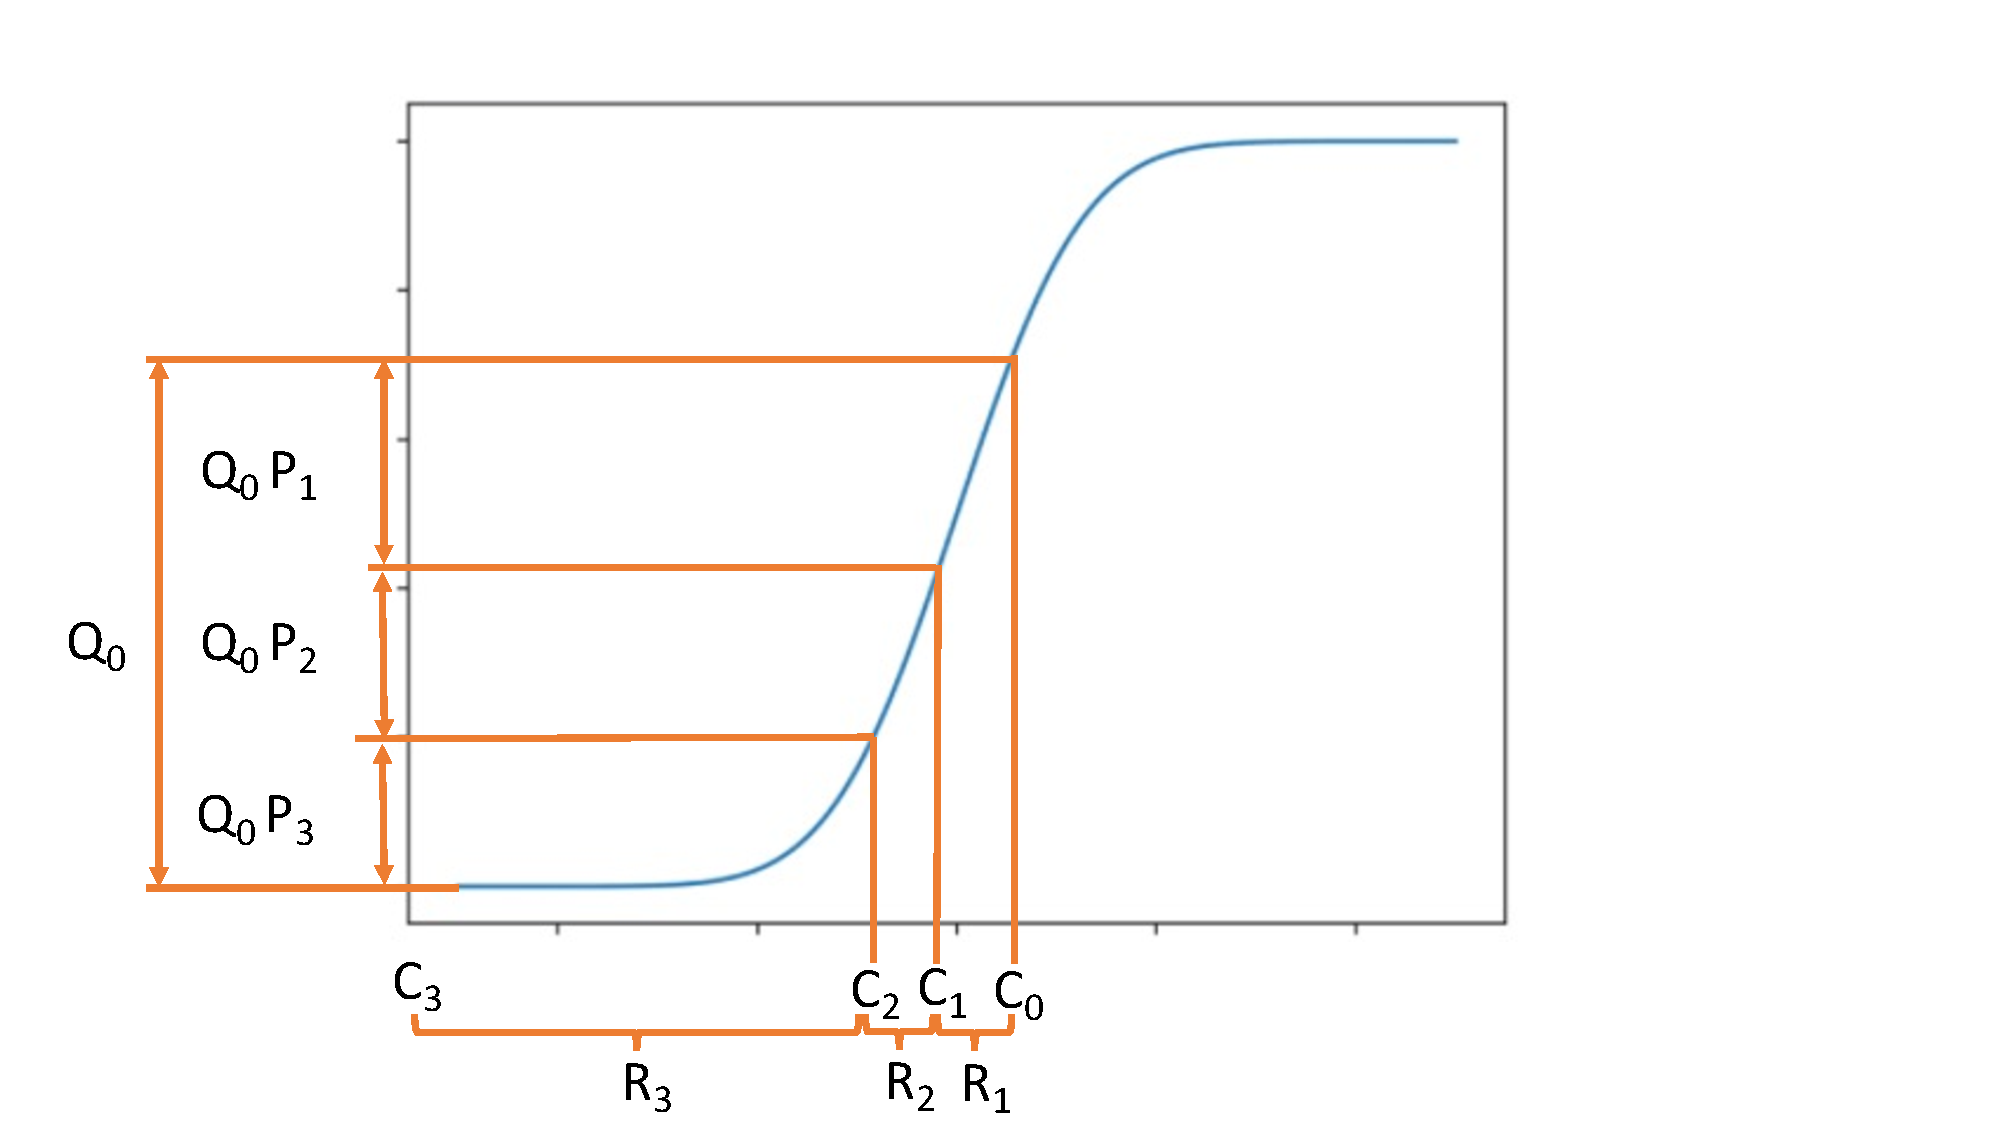
\includegraphics[scale=0.4]{pricing/cr_cdo_copula.pdf}
\end{center}
\caption{Probabilities, thresholds and recovery rates. }
\label{fig_copula}
\end{figure}

The Gaussian assumption for $Y_i$, $Z_i$ and $M$ then leads to the following probabilities
conditional on the common factor $M$:
\begin{itemize}
\item Probability of default
$$
P_i(M) := \P(t_i \leq t|M) = \P(Y_i \leq C_{i,0}(t)|M) = N \left( \frac{C_{i,0}(t) - a_i\,M}{\sqrt{1-a_i^2}}\right) 
$$
as in the standard Gaussian Copula case
\item Probability of recovery rate $r_{ij}$ given default of entity $i$
$$
  P_{i,j}(M) := \frac{\P(C_{i,j}(t) < Y_i \leq C_{i, j-1}(t) | M)}{\P(Y_i \leq C_{i,0}(t)|M)} 
  = \frac{ N \left( \frac{C_{i,j-1}(t) - a_i\,M}{\sqrt{1-a_i^2}}\right) - N \left( \frac{C_{i,j}(t) - a_i\,M}{\sqrt{1-a_i^2}}\right) }{ N \left( \frac{C_{i,0}(t) - a_i\,M}{\sqrt{1-a_i^2}}\right) }
  $$
\item Probability of default with recovery rate $r_{ij}$ 
  $$
  P_{i,j}(M)\times P_i(M) =  N \left( \frac{C_{i,j-1}(t) - a_i\,M}{\sqrt{1-a_i^2}}\right) - N \left( \frac{C_{i,j}(t) - a_i\,M}{\sqrt{1-a_i^2}}\right)
$$
\end{itemize}

The distribution of portfolio losses, conditional on $M$
$$
L(M) = \sum_{i=1}^N N_i\,(1-R_i(M))\,P_i(M) 
$$
is then computed by convolution. As in the single-recovery case we want to use a bucketing algorithm when loss amounts and default probabilities are allowed to differ across entities.
The {\em Hull-White Bucketing Algorithm} in \cite{HullWhiteBucketing} was extended slightly to handle the multi-recovery case.

\subsubsection{Calibration of default curves for index tranches}

If we calculate the npv of an Index CDS based on the underlying constituent CDS spread curves we notice a basis between the intrisinc value and the quoted index spread.
The basis and two methods to adjust the underlying curves to close the basis are described in detail in \cite{okane2008}.
Our calibration method is based on the idea of the Forward Default Probability Multiplier.

Instead of a calibration of the underlying curves to all quoted index terms in a iterative method and using a termstructure of adjustment factors, we are using a simpler method with a flat adjustment factor $\lambda$.

Let $Q_i(t)$ the survival probability of the i-th constituent at time t. Their adjusted survival probability is given by $\tilde{Q_i(t)}=Q_i(t)^\lambda$.

When we are pricing a index CDS tranche, we set the factor $\lambda$ so that the intrinsic valuation of the underlying index CDS with the adjusted curves matches the quoted price.





\subsubsection{RPA}
\label{pricing:cr_rpa}

The premium leg of a RPA is priced by discounting premium payments adjusted for default probability, its net present
value can be written

\begin{equation}
F = \sum_{i=1}^{n} f_i P_{OIS}(T_i) S(T_i) + A
\end{equation}

with

\begin{itemize}
\item $f_i$ the future payable fee amounts, $i=1,\ldots,n$
\item $T_i$ the payment time of the fee $f_i$, $i=1,\ldots,n$
\item $P_{OIS}(t)$ the discount factor on the relevant OIS curve (in a collateralised RPA)
\item $S(T_i)$ the survival probability of the reference entity between today and $T_i$
\item $A$ is the value of the fee accruals, see below
\end{itemize}

If the premium payments are given as simple cashflows, $A=0$. If on the other hand the premium payments are {\em
  coupons} and the RPA agreement specifies the payment of accruals in case of a default event, the value of the fee
accruals is computed as

\begin{equation}
  A = \sum_{i=1}^{n} a_i P_{OIS}(T_i^{\text{mid}}) P_{\text{def}}(A^s_i,A^e_i)
\end{equation}

using the mid-point rule, where

\begin{itemize}
\item $T_i^{\text{mid}}$ is the mid point between
\begin{itemize}
\item $A^s_i$ defined as the greater of the accrual start date and the evaluation date and
\item $A^e_i$ the accrual end date
\end{itemize}
\item $a_i$ are the accruals of $f_i$ between $A^s_i$ and the date corresponding to $T_i^{\text{mid}}$
\item $P_{\text{def}}(A^s_i,A^e_i)$ is the probably of default of the reference entity between $A^s_i$ and $A^e_i$
\end{itemize}

The protection leg of a RPA is priced using different methods, depending on the structure of the underlying. See section
\ref{input:cr_rpa} for the detailed criteria that are used to pick the pricing method depending on the trade xml
representation:

\begin{itemize}
\item Vanilla Swap: Analytic Pricer using a European swaption representation of the underlying EPE profile
\item Strucutred Swap: Numeric LGM Pricer
\item Callable Swap / Swaption: Numeric LGM Pricer
\item Cross Currency Swap: Analytic Pricer using a FX Option representation of the underlying EPE profile
\item Treasury Lock: Numeric LGM Pricer
\end{itemize}

\underline{Analytic Pricer using European swaption representation:}

The protection leg is priced as a weighted sum over European swaptions

\begin{equation}
P = \sum_{i=1}^{N} p (1-R) P_{\text{def}}(W^s_i,W^e_i) \nu(W_i)
\end{equation}

where

\begin{itemize}
\item $W_i$ is a swaption with expiry $t_i$ representing the option to enter into the cashflows of the underlying swap
  with payment date greater than $t_i$. The swaption is found by matching the NPV, Delta and Gamma of the exercise-into
  underlying swap within a LGM1F model at a suitable expansion point for the LGM state with the NPV, Delta and Gamma of
  a standard underlying.
\item $P_{\text{def}}(W^si, W^e_i)$ is the probability of default of the reference entity between $W^s_i$ and $W^e_i$
\item $R$ is the assumed recovery rate, or the fixed recovery rate from the RPA termsheet, if given
\item $p$ is the participation rate
\item $\nu(W_i)$ is the NPV as of the evaluation date of the swaption $W_i$
\end{itemize}

The intervals $[W^s_i, W^e_i]$ and swaption expiries $t_i \in [W^s_i, W^e_i]$, $i=1,\ldots,N$ are chosen such that the
intervals cover the interval between

\begin{itemize}
\item the greater of the protection start and evaluation date and
\item the earlier of the protection end date and the latest underlying swap payment date
\end{itemize}

One possible concrete choice in the case of a vanilla fix versus float underlying (with a float
coupon frequency being a multiple of the fixed coupon frequency) is

\begin{itemize}
\item $W^s_i$ the maximum of the evaluation date, protection start date and $i$th underlying float accrual start date
\item $W^e_i$ the minimum of the protection end date and the $i$th underlying accrual end date
\item $t_i$ is the mid point between suitable dates $W^s_i$ and $W^e_i$ (see below)
\end{itemize}

where only non-empty periods $[W^s_i, W^e_i]$ are kept.

Notice that the protection leg of a RPA is identical to a protection leg of a CDS with nominal $V$ if $\nu(W_i)$ is
replaced by a constant amount $V$. The total NPV of an RPA is given as

\begin{equation}
\text{NPV}_{\text{RPA}} = F - P
\end{equation}

for a protection seller position resp.

\begin{equation}
\text{NPV}_{\text{RPA}} = P - F
\end{equation}

for a protection buyer position.

\underline{Analytic Pricer using FX Option representation:}

The approach is similar to ``Analytic Pricer using European swaption representation'', but in this case the
exercise-into flows of the underlying are matched with FX Spot Trades using the NPV and FX Delta. This matching can be
performed in a model independent way, interest rates are assumed to be deterministic here.

\underline{Numeric LGM Pricer}

The EPE is computed in a LGM1F model. The approach is very similar to the pricing of bermudan swaptions. The calibration
approach is also the same for swap underlyings. For ``Treasury Lock'' underlying a Coterminal ATM calibration is used.

\subsubsection{Credit Linked Swap}

A credit linked swap is priced using a discounted cashflow approach assuming independent interest and credit rates.

Payments that are made independent of credit events for the reference CDS are priced just as in a vanilla interest rate
swap, see \ref{pricing:ir_irs}.

The NPV of payments that are only made if no credit event has occured until the payment date are weighted in addition
with the survival probability for the payment date. If accruals are settled on the event date, it is assumed that
defaults occur on the midpoint of the coupon period, i.e. that (on average) half of the accruals are paid and discounted
from the midpoint of the coupon period. This is in analogy to premium payment pricing in CDS, see \ref{pricing:cr_cds}.

Payments that are made in case of a credit event are priced in analogy to protection payments in CDS, see
\ref{pricing:cr_cds}. The discretisation grid is given by the payment dates of the respective legs, refined by
additional points to ensure a minimum number of grid points per year as specified in the pricing engine parameter
\verb+TimeStepsPerYear+.

The pricing engine provides the following additional results:

\begin{itemize}
\item npv\_independent: The NPV of the payments that are made independent of credit events.
\item npv\_credit\_linked: The NPV of the payments that are made only if no credit event has occured until the payment date.
\item npv\_credit\_linked\_accruals: The NPV of the accruals of the credit linked payments, if accruals are settled.
\item npv\_default\_payments: The NPV of the payments triggered by a credit event, weighted by $(1-rr)$ where $rr$ is
  the applicable recovery rate.
\item npv\_recovery\_payments: The NPV of the payments triggered by a credit event, weighted by $rr$.
\end{itemize}

%- - - - - - - - - - - - - - - - - - - - - - - - - - - - - - - - - - - - - - - - - - - - - - - - - - - - - 
\subsection{Commodity Derivatives}
\subsubsection{Commodity Forward}
\label{pricing:com_forward}

The commodity forwarding curve is used for respective underlying commodity. 
The net present value of a commodity forward can be priced discounting the 
cashflows at maturity as per:
$$
\NPV = \mbox{Quantity}\cdot \omega\cdot (F(0,T) - K) \cdot P(T)
$$
where:
\begin{itemize}
\item Quantity: number of units of the underlying commodity
\item $K$: strike price
\item $F(0,T)$: the forward commodity price for maturity $T$ at time 0 (valuation date)
\item $P(T)$: the discount factor for maturity time $T$
\item $\omega$: 1 for a forward to buy commodity, -1 for a forward to sell a commodity 
\end{itemize}

\subsubsection{European Commodity Option}
\label{pricing:com_option}

European Commodity Options are priced using the Black-Scholes model with log-normal 
volatilities. Volatility structures with smile are taken into account where available. 
The commodity forwarding curve is used for respective commodity.

The Black-Scholes model assumes that the spot commodity price C follows Geometric 
Brownian Motion:
$$
dC/C=\mu(t)dt + \sigma(t)\,dW
$$
The model?s drift is calibrated such that the expected future spot commodity price 
agrees with today?s fair forward commodity price for time T. This means that the 
commodity forward rate $F(t,T)$ follows drift-free GBM under the T-forward measure:
$$
dF(t,T)) = \sigma(t)\,F(t,T)\,dW
$$
This leads a Black76 analytical solution for the present value of a European FX option:
$$
\NPV = N\cdot \mbox{Black}(K, F(0,T), \sigma\sqrt{T},\omega)\cdot?P(T)
$$
where:
\begin{itemize}
\item $N$: notional
\item $K$: strike price
\item $F(0,T)$: the forward commodity price for maturity $T$ at time 0 (start)
\item $\sigma$: the volatility of the commodity forward price
\item $\omega$: 1 for a call option, -1 for a put option
\item $P(T)$: the discount factor for maturity time $T$
\end{itemize}

See Black Model, Section \ref{sec:models}, for more details.


\subsubsection{Commodity Futures Option}
\label{pricing:com_futuresoption}

Though Commodity Futures Options can be technically American style
 (as e.g. in the case of base metal futures options at LME),
we treat them as European options following \cite{Clark_2014}.

The option payoff on option exercise date $t_e$ with underlying futures
contract expiry $T>t_e$  is
$$
\NPV(t_e) = N\cdot \left(\omega(F(t_e, T) - K)\right)^+.
$$
We assume that the futures price follows Geometric Brownian Motion:
$$
dF(t,T)) = \sigma(t)\,F(t,T)\,dW.
$$
This leads to a Black76 analytical solution for the present value of
the Futures Option:
$$
\NPV = N\cdot \mbox{Black}(K, F(0,T), \sigma\sqrt{t_e},\omega)\cdot P(T)
$$
where:
\begin{itemize}
\item $N$: notional (units of the underyling futures contract)
\item $K$: strike price
\item $F(0,T)$: the futures price for contract expiry $T$ at time 0 (start)
\item $\sigma$: the volatility of the commodity futures price
\item $\omega$: 1 for a call option, -1 for a put option
\item $P(T)$: the discount factor for the underlying futures expiry $T$
\end{itemize}

See Black Model, Section \ref{sec:models}, for more details.

\subsubsection{Commodity Swap}
\label{pricing:com_swap}

As in Section \ref{pricing:com_forward}, the commodity forwarding
curve is used for respective underlying commodity.
 The net present value of each calculation period in a Commodity Swap 
can be computed following \cite{Clark_2014}:
$$
\NPV_{Period} = \mbox{Quantity}\cdot \omega\cdot \left(\frac{1}{n}\sum_{i=1}^n F(0,T_i) - K\right) \cdot P(T)
$$
where:
\begin{itemize}
\item Quantity: number of units of the underlying commodity
\item $K$: strike price
\item the sum runs over all fixing dates $t_i$ in the calculation
  period, $i=1, ..., n$
\item $F(0,T_i)$: the forward commodity price for maturity $T_i$ seen at
  time 0 (valuation date), $T_i$ is the prompt futures expiry date
  associated with the fixing date $t_i$ if the Swap references Futures
  prices, or it is the fixing date $t_i$ if the  Swap references
  Commodity spot prices.
\item $P(T)$: the discount factor for settlement date $T$ typically 5
  business days after the last fixing date in the period
\item $\omega$: +1 for a long Commodity Swap, -1 otherwise 
\end{itemize}

As the payoff can also be rolled up into a single payment we
generalize the pricing formula, taking the sum over all fixings dates
in all calculation periods
$$
\NPV_{Total} = \mbox{Quantity}\cdot \omega\cdot \frac{1}{N}\sum_{i=1}^N\left( F(0,T_i) - K\right) \cdot P(T^{Set}_i)
$$
where $T^{Set}_i$ denotes the settlement date associated with each fixing,
possibly linked to the following period end or swap maturity.
\subsubsection{Commodity Basis Swap}
\label{pricing:com_basisswap}

The net present value of each calculation period in a Commodity Basis Swap 
can be computed following \cite{Clark_2014}, and slightly extending
Section \ref{pricing:com_swap}
:
$$
\NPV = \mbox{Quantity}\cdot \omega\cdot \frac{1}{N}\sum_{i=1}^n
  \left(F^{(1)}(0,T_i) - F^{(2)}(0,T_i) - K\right) \cdot P(T_i^{Set})
$$
where:
\begin{itemize}
\item Quantity: number of units of the underlying commodity
\item $K$: strike price
\item the sum runs over all fixing dates $t_i$ across all calculation
  periods, $i=1, ..., N$
\item $F^{(1,2)}(0,T_i)$: the forward price of commodity 1 resp. 2 for
  maturity $T_i$ seen at time 0 (valuation date), $T_i$ is the prompt
  futures expiry date  associated with the fixing date $t_i$ if the
  Swap references Futures  prices, or it is the fixing date $t_i$ if
  the  Swap references Commodity spot prices.
\item $P(T_i^{Set})$: the discount factor for settlement date
  following fixing date $T_i$, possibly a number of business days
  (typically five) past the next calculation period end, or past the
  Swap's final calculation period  end if all payouts are rolled up
  into a single payment 
\item $\omega$: +1 for a long Commodity Swap, -1 otherwise 
\end{itemize}

\subsubsection{Commodity Swaption - Future Settlement Prices}
\label{pricing:com_swaption_future_settlement_prices}

This section describes the European swaption pricing when the underlying swap references commodity future settlement prices. In particular, we consider the case where on each pricing date on the commodity floating leg of the underlying swap, the settlement price of the prompt future contract is observed. The calculations can be easily generalised to a non-prompt future contract.

We assume that there are $N$ future contracts and, following Section 2.2 of \cite{Clark_2014}, we assume that each future contract price follows a driftless lognormal process under the risk neutral measure in the domestic currency
\begin{equation}
\label{eq:comm_future_price_processes}
dF_{\alpha}(t) = \sigma_{\alpha} F_{\alpha}(t) dW_{\alpha}(t)
\end{equation}
where $\alpha = 1, \ldots, N$, $0 \leq t \leq s_{\alpha}$ and $s_{\alpha}$ in the expiry date of the $\alpha$-th future contract. Additionally, we assume that the correlation between any two future price processes is driven by an instantaneous correlation between their two driving Brownian motions. In particular, we assume that
\begin{equation}
d \langle W_{\alpha}(t), W_{\gamma}(t) \rangle = \rho_{\alpha, \gamma}
\end{equation}
for $1 \leq \alpha < \gamma \leq N$. Instead of providing a full correlation matrix, it is convenient in certain cases to parameterise the correlation. In ORE+, we allow for a parameterisation of the form
\begin{equation}
\rho_{\alpha, \gamma} = \exp \left\{ -\beta \left( s_{\gamma} - s_{\alpha} \right) \right\}
\end{equation}
where $\beta \geq 0$ and a value of $\beta$ equal to $0$ gives an instantaneous correlation of $1$ between all future contract price processes.

We can now write down some straightforward properties of the future price processes that we will use later
\begingroup
\addtolength{\jot}{0.5em}
\begin{align}
F_{\alpha}(t) &= F_{\alpha}(0) \exp \left\{ - \frac{1}{2} \sigma^2_{\alpha} t + \sigma_{\alpha} W_{\alpha}(t) \right\} \\
\Ex{F^2_{\alpha}(t)} &= F^2_{\alpha}(0) \exp \left\{ \sigma^2_{\alpha} t \right\} \label{eq:future_second_moment} \\
\Ex{F_{\alpha}(t)F_{\gamma}(t)} &= F_{\alpha}(0) F_{\gamma}(0) \exp \left\{ \rho_{\alpha, \gamma} \sigma_{\alpha} \sigma_{\gamma} t \right\} \label{eq:future_exp_product}
\end{align}
\endgroup

We now define the commodity swap underlying the commodity swaption that we are valuing. The commodity swap will exchange a sequence of payments that depend on known fixed prices, the commodity fixed leg, against a sequence of payments that reference the settlement prices of the future contracts, the commodity floating leg. The swap has $n$ calculation periods denoted by $I_1, \ldots, I_n$. Associated with the $i$-th calculation period, $I_i$, we have the commodity quantity for the calculation period denoted by $N_i$, the fixed leg price denoted by $K_i$ and the payment date denoted by $\tau_i$. On the commodity floating leg, each calculation period, $I_i$, contains $n_i$ pricing dates $t_{i,1}, \ldots, t_{i, n_i}$. On each pricing date, the settlement price of the prompt future contract is observed. To associate a pricing date $t_{i,j}$, $j = 1, \ldots, n_i$ with its prompt future contract we define the function $T:[0, +\infty) \to \{ 0, 1, \ldots, N \}$. This function takes a pricing date and returns the index of the future contract whose settlement price is to be observed. In particluar, this function also defines the roll date convention which can be specified on commodity swap contracts that have a floating leg with averaging. We now define the floating price associated with each calculation period, $I_i$, as
\begin{equation}
\frac{1}{n_i} \sum_{j=1}^{n_i} F_{T(t_{i,j})}(t_{i,j})
\end{equation}
Note that we can have $n_i = 1$ for $i = 1, \ldots, n$. In this case, we have a non-averaging commodity floating leg. In other words, the commodity future contract settlement price is observed on a single date in the calculation period to determine the floating price for the calculation period. If $n_i > 1$, the calculation period $I_i$ is an averaging period. In general, a commodity swap will be either non-averaging or averaging. In the case of averaging swaps, the pricing dates for a calculation period are generally defined as being every business day in the calculation period. The payoff $\Pi_i$ on payment date $\tau_i$ for a commodity swap defined in this way is given by
\begin{equation}
\Pi_i = \omega \left[ \frac{1}{n_i} \sum_{j=1}^{n_i} F_{T(t_{i,j})}(t_{i,j}) - K_i \right] N_i
\end{equation}
where $\omega$ is $1$ for a payer swap and $-1$ for a receiver swap.

We now assume that we have a European swaption on the swap defined above with exercise date $t_e$ where $t_e < t_{1,1}$. We assume in what follows that we have deterministic domestic interest rates with $P(t,T)$ denoting the discount factor at time $t$ for maturity $T$. The value of the swap, $\hat{V}(t_e)$, at time $t_e$ is therefore given by
\begin{equation}
\label{eq:value_swap_te}
\begin{split}
\hat{V}(t_e) &= \omega \sum_{i=1}^{n} P(t_e, \tau_i) \frac{N_i}{n_i} \sum_{j=1}^{n_i} \CEx{F_{T(t_{i,j})}(t_{i,j})}{\mathcal{F}_{t_e}} \\
             &\qquad - \omega \sum_{i=1}^{n} P(t_e, \tau_i) K_i N_i \\
             &= \omega \sum_{i=1}^{n} P(t_e, \tau_i) \frac{N_i}{n_i} \sum_{j=1}^{n_i} F_{T(t_{i,j})}(t_e) - \omega \sum_{i=1}^{n} P(t_e, \tau_i) K_i N_i
\end{split}
\end{equation}
We note that the first term in \eqref{eq:value_swap_te} is the value of the swap's floating leg at $t_e$ and the second term is the value of the swap's fixed leg at $t_e$.

Now, the value of the swaption, $V(0)$, at time zero is given by
\begin{equation}
\label{eq:value_swaption_t0}
V(0) = P(0, t_e) \Ex{\hat{V}(t_e)^{+}}
\end{equation}
Monte Carlo simulation would be one option for calculating a value for the expectation in \eqref{eq:value_swaption_t0}.

Following Section 2.7.4.2 of \cite{Clark_2014}, we can calculate an approximate value for the expectation in \eqref{eq:value_swaption_t0} by replacing the floating leg with a lognormally distributed random variable $X$ whose first and second moments match those of the floating leg. Formally, we define
\begin{equation}
A(t_e) = \sum_{i=1}^{n} P(t_e, \tau_i) \frac{N_i}{n_i} \sum_{j=1}^{n_i} F_{T(t_{i,j})}(t_e)
\end{equation}
and let $X \sim LN(\mu_X, \sigma^2_X t_e)$ where we impose the conditions
\begingroup
\addtolength{\jot}{0.5em}
\begin{align}
\Ex{A(t_e)} &= \Ex{X} = \exp \left\{ \mu_X + \frac{1}{2} \sigma^2_X t_e \right\} \\
\Var{A(t_e)} &= \Var{X} = \left[ e^{\sigma^2_X t_e} - 1 \right] \Ex{X}^2
\end{align}
\endgroup
which yields
\begingroup
\addtolength{\jot}{0.5em}
\begin{align}
\sigma_X &= \sqrt{ \frac{1}{t_e} \ln \frac{\Ex{A^2(t_e)}}{\Ex{A(t_e)}^2} } \label{eq:future_sigma_x} \\
\mu_X &= \ln \Ex{A(t_e)} - \frac{1}{2} \sigma^2_X t_e \label{eq:future_mu_x}
\end{align}
\endgroup
Now, defining the value of the fixed commodity leg at $t_e$ as
\begin{equation}
K^{*} = \sum_{i=1}^{n} P(t_e, \tau_i) K_i N_i
\end{equation}
we can write the approximate value, $\tilde{V}(0)$, of the swaption at time zero as
\begin{equation}
\tilde{V}(0) = P(0, t_e) \Ex{\left[ \omega \left( X - K^{*} \right) \right]^{+}}
\end{equation}
This is the familiar expectation that appears in the Black-76 model as outlined in Section \ref{models:black}. In particular, using the $\text{Black}$ function defined in Section \ref{models:black}, we have
\begin{equation}
\tilde{V}(0) = P(0, t_e) \text{Black} \left( K^{*}, \Ex{A(t_e)}, \sigma_X \sqrt{t_e}, \omega \right)
\end{equation}

All that remains is to write down the explicit value for $\Ex{A(t_e)}$ and $\Ex{A^2(t_e)}$ appearing in \eqref{eq:future_sigma_x} and \eqref{eq:future_mu_x}. It is clear that
\begin{equation}
\label{eq:exp_A_te}
\Ex{A(t_e)} = \sum_{i=1}^{n} P(t_e, \tau_i) \frac{N_i}{n_i} \sum_{j=1}^{n_i} F_{T(t_{i,j})}(0)
\end{equation}
In order to calculate $\Ex{A^2(t_e)}$, we write down an explicit expression for $A^2(t_e)$
\begin{equation}
\begin{split}
& A^2(t_e) = \sum_{i=1}^{n} P^2(t_e, \tau_i) \frac{N^2_i}{n^2_i} \left[ \sum_{j=1}^{n_i} F_{T(t_{i,j})}(t_e) \right]^2 \\
         &\quad + 2 \sum_{k=2}^{n} \sum_{i=1}^{k-1} P(t_e, \tau_k) P(t_e, \tau_i) \frac{N_k N_i}{n_k n_i} \left[ \sum_{j=1}^{n_k} F_{T(t_{k,j})}(t_e) \sum_{l=1}^{n_i} F_{T(t_{i,l})}(t_e) \right]
\end{split}
\end{equation}
which in turn gives
\begin{equation}
\label{eq:future_A_te_2}
\begin{split}
& A^2(t_e) = \sum_{i=1}^{n} P^2(t_e, \tau_i) \frac{N^2_i}{n^2_i} \left[ \sum_{j=1}^{n_i} F^2_{T(t_{i,j})}(t_e) \right. \\
         &\quad + \left. 2 \sum_{k=2}^{n_i} \sum_{l=1}^{k-1} F_{T(t_{i,k})}(t_e) F_{T(t_{i,l})}(t_e) \right] \\
         &\quad + 2 \sum_{k=2}^{n} \sum_{i=1}^{k-1} P(t_e, \tau_k) P(t_e, \tau_i) \frac{N_k N_i}{n_k n_i} \left[ \sum_{j=1}^{n_k} \sum_{l=1}^{n_i} F_{T(t_{k,j})}(t_e) F_{T(t_{i,l})}(t_e) \right]
\end{split}
\end{equation}
Now, taking the expectation and using \eqref{eq:future_second_moment} and \eqref{eq:future_exp_product}, we get
\begin{equation}
\label{eq:exp_future_A_te_2}
\begin{split}
& \Ex{A^2(t_e)} = \sum_{i=1}^{n} P^2(t_e, \tau_i) \frac{N^2_i}{n^2_i} \left[ \sum_{j=1}^{n_i} F^2_{T(t_{i,j})}(0) \exp \left\{ \sigma^2_{T(t_{i,j})} t_e \right\} \right. \\
              &\quad \left. + 2 \sum_{k=2}^{n_i} \sum_{l=1}^{k-1} F_{T(t_{i,k})}(0) F_{T(t_{i,l})}(0) \exp \Big\{ \rho_{T(t_{i,k}), T(t_{i,l})} \sigma_{T(t_{i,k})} \sigma_{T(t_{i,l})} t_e \Big\} \right] \\
              &\quad + 2 \sum_{k=2}^{n} \sum_{i=1}^{k-1} P(t_e, \tau_k) P(t_e, \tau_i) \frac{N_k N_i}{n_k n_i} \bigg[ \sum_{j=1}^{n_k} \sum_{l=1}^{n_i} F_{T(t_{k,j})}(0) \bigg. \\
              &\qquad \qquad \bigg. F_{T(t_{i,l})}(0) \exp \Big\{ \rho_{T(t_{k,j}), T(t_{i,l})} \sigma_{T(t_{k,j})} \sigma_{T(t_{i,l})} t_e \Big\} \bigg]
\end{split}
\end{equation}

\underline{FX adjustment}

If the underlying swap references a commodity quoted in a currency different from the swaption currency we must adjust \eqref{eq:exp_A_te} and \eqref{eq:exp_future_A_te_2} accordingly.

We assume that the FX Spot rate $Z$  follows a Geometric Brownian Motion:
\begin{equation}
\label{eq:fx_rate_dynamics}
\begin{split}
dZ/Z = \mu_{Z}(t)dt + \sigma_{Z}(t) dW_{Z}
\end{split}
\end{equation}

For simplicity we assume that $\sigma_{Z}=0$ and the adjustment involves converting each futures price with the FX-forward at the price observation time. For completeness we write out the required adjustments.

The floating price associated with each calculation period, $I_i$, becomes
\begin{equation}
\frac{1}{n_i} \sum_{j=1}^{n_i} F_{T(t_{i,j})}(t_{i,j}) Z(t_{i,j})
\end{equation}

And we have:

\begingroup
\addtolength{\jot}{0.5em}
\begin{align}
\Ex{F_{\alpha}(t)Z(t)} &= F_{\alpha}(0) Z(0) \exp \left\{ (r_d - r_f) t + \rho_{F_{\alpha}, Z} \sigma_{F_{\alpha}} \sigma_{Z} t \right\} \label{eq:future_fx_exp_product} \\
\Ex{F^2_{\alpha}(t)Z^2(t)} &= F^2_{\alpha}(0)Z^2(0) \exp \left\{ 2 (r_d - r_f) t + \sigma^2_{\alpha} t + \sigma^2_{Z} t + 4 \rho_{F_{\alpha}, Z} \sigma_{F_{\alpha}} \sigma_{Z} t \right\} \label{eq:future_fx_square}
\end{align}
\endgroup

\eqref{eq:value_swap_te} becomes:
\begin{equation}
\label{eq:value_swap_te_fx}
\begin{split}
\hat{V}(t_e) = \omega \sum_{i=1}^{n} P(t_e, \tau_i) \frac{N_i}{n_i} \sum_{j=1}^{n_i} F_{T(t_{i,j})}(t_e) Z(t_{i,j}) - \omega \sum_{i=1}^{n} P(t_e, \tau_i) K_i N_i
\end{split}
\end{equation}

As before, we can calculate an approximate value for the expectation in (\eqref{eq:value_swap_te_fx}) by replacing the Floating leg with a lognormally distributed random variable X whose first and second moments match those of the floating leg, with:
\begin{equation}
A(t_e) = \sum_{i=1}^{n} P(t_e, \tau_i) \frac{N_i}{n_i} \sum_{j=1}^{n_i} F_{T(t_{i,j})}(t_e) Z(t_{i,j})
\end{equation}

Using \eqref{eq:future_fx_exp_product}, with $\sigma_{Z}=0$, we get:
\begin{equation}
\label{eq:exp_A_te_fx}
\begin{split}
\Ex{A(t_e)} &= \sum_{i=1}^{n} P(t_e, \tau_i) \frac{N_i}{n_i} \sum_{j=1}^{n_i} F_{T(t_{i,j})}(0) Z(t_e) \exp \left\{ (r_d(t_e, t_{i,j}) - r_f(t_e, t_{i,j})) (t_{i,j} - t_e) \right\} \\
            &= \sum_{i=1}^{n} P(t_e, \tau_i) \frac{N_i}{n_i} \sum_{j=1}^{n_i} F_{T(t_{i,j})}(0) Z(t_e, t_{i,j}) 
\end{split}
\end{equation}

where $Z(t_1, t_2)$ is projected forward FX rate. And:
\begin{equation}
\label{eq:exp_future_A_te_2_te_fx}
\begin{split}
& \Ex{A^2(t_e)} = \sum_{i=1}^{n} P^2(t_e, \tau_i) \frac{N^2_i}{n^2_i} \left[ \sum_{j=1}^{n_i} F^2_{T(t_{i,j})}(0)Z^2(t_e,t_{i,j}) \exp \left\{ \sigma^2_{T(t_{i,j})} t_e \right\} \right. \\
              &\quad \left. + 2 \sum_{k=2}^{n_i} \sum_{l=1}^{k-1} F_{T(t_{i,k})}(0)Z(0,t_{i,k}) F_{T(t_{i,l})}(0)Z(t_e,t_{i,l}) \exp \Big\{ \rho_{T(t_{i,k}), T(t_{i,l})} \sigma_{T(t_{i,k})} \sigma_{T(t_{i,l})} t_e \Big\} \right] \\
              &\quad + 2 \sum_{k=2}^{n} \sum_{i=1}^{k-1} P(t_e, \tau_k) P(t_e, \tau_i) \frac{N_k N_i}{n_k n_i} \bigg[ \sum_{j=1}^{n_k} \sum_{l=1}^{n_i} F_{T(t_{k,j})}(0) Z(t_e,t_{k,j}) \bigg. \\
              &\qquad \qquad \bigg. F_{T(t_{i,l})}(0) Z(t_e,t_{i,l}) \exp \Big\{ \rho_{T(t_{k,j}), T(t_{i,l})} \sigma_{T(t_{k,j})} \sigma_{T(t_{i,l})} t_e \Big\} \bigg]
\end{split}
\end{equation}


\subsubsection{Commodity Swaption - Spot Prices}
\label{pricing:com_swaption_spot_prices}

This section describes the European swaption pricing when the underlying swap references a commodity spot price. In particular, we consider the case where on each pricing date on the commodity floating leg of the underlying swap, the spot price of a commodity is observed.

Following Section 2.2.5 of \cite{Clark_2014}, we assume that the spot price process under the risk neutral measure in the domestic currency is given by
\begin{equation}
\label{eq:comm_spot_price_process}
dS(t) = \left[ r(t) - r_f(t) \right] S(t) dt + \sigma_{S}(t) S(t) dW(t)
\end{equation}
where $r(t)$, $r_f(t)$ and $\sigma_{S}(t)$ are deterministic with $r(t)$ being the risk free domestic rate, $r_f(t)$ the commodity convenience yield and $\sigma_{S}(t)$ the instantaneous volatility. Note that we have
\begin{equation}
P(t, T) = \exp \left\{ -\int_t^T r(u) du \right\}
\end{equation}
for $0 \leq t \leq T < +\infty$ where $P(t, T)$ is as defined in Section \ref{pricing:com_swaption_future_settlement_prices} above.

We can now write down some straightforward properties of the spot price process that we will use later. Solving the SDE for $S(t)$, we get
\begin{equation}
\begin{split}
S(t_2) &= S(t_1) \exp \left\{ \int_{t_1}^{t_2} r(u) - r_f(u) du \right. \\
       &\qquad + \left. \int_{t_1}^{t_2} \sigma_S(u) dW(u) - \frac{1}{2} \int_{t_1}^{t_2} \sigma^2_S(u) du \right\}
\end{split}
\end{equation}
for $0 \leq t_1 \leq t_2 < +\infty$. The expected value at $t_2$ given information up to and including $t_1$ follows immediately 
\begin{equation}
\CEx{S(t_2)}{\mathcal{F}_{t_1}} = S(t_1) \exp \left\{ \int_{t_1}^{t_2} r(u) - r_f(u) du \right\} \label{eq:spot_exp_value}
\end{equation}
It will also be useful to look at $S^2(t)$ which is given by
\begin{equation}
\begin{split}
S^2(t_2) &= S^2(t_1) \exp \left\{ 2 \int_{t_1}^{t_2} r(u) - r_f(u) du + \int_{t_1}^{t_2} \sigma^2_S(u) du \right. \\
         &\qquad + \left. \int_{t_1}^{t_2} 2 \sigma_S(u) dW(u) - \frac{1}{2} \int_{t_1}^{t_2} \left(2 \sigma_S(u) \right)^2 du \right\}
\end{split}
\end{equation}
with associated conditional expected value
\begin{equation}
\CEx{S^2(t_2)}{\mathcal{F}_{t_1}} = S^2(t_1) \exp \left\{ 2 \int_{t_1}^{t_2} r(u) - r_f(u) du + \int_{t_1}^{t_2} \sigma^2_S(u) du \right\} \label{eq:spot_second_moment}
\end{equation}
Note that the value of a $T$-maturity long forward contract on the commodity at time $t$ with strike $K$ is given by
\begin{equation}
V_f(t, T) = P(t, T) \CEx{S(T) - K}{\mathcal{F}_{t}} \label{eq:spot_forward_value}
\end{equation}
We denote by $F(t, T)$ the value of $K$ that gives the contract a value of zero at time $t$. This quantity is the $T$-maturity forward rate. It is clear from this and \eqref{eq:spot_exp_value} that
\begin{equation}
F(t, T) = \CEx{S(T)}{\mathcal{F}_{t}} = S(t) \exp \left\{ \int_{t}^{T} r(u) - r_f(u) du \right\} \label{eq:spot_forward_rate}
\end{equation}
One final quantity that will be useful in subsequent calculations below is the expectation of the product of commodity prices at two separate times. In particular, using the tower property of conditional expectation, \eqref{eq:spot_exp_value} and \eqref{eq:spot_second_moment}
\begin{equation}
\label{eq:comm_spot_exp_product}
\begin{split}
\CEx{S(t_2)S(t_3)}{\mathcal{F}_{t_1}} &= \CEx{ \CEx{S(t_2)S(t_3)}{\mathcal{F}_{t_2}} }{\mathcal{F}_{t_1}} \\
&= \CEx{S(t_2) \CEx{S(t_3)}{\mathcal{F}_{t_2}} }{\mathcal{F}_{t_1}} \\
&= \CEx{S^2(t_2) \exp \left\{ \int_{t_2}^{t_3} r(u) - r_f(u) du \right\} }{\mathcal{F}_{t_1}} \\
&= F(t_1, t_2) F(t_1, t_3) \exp \left\{ \int_{t_1}^{t_2} \sigma^2_S(u) du \right\}
\end{split}
\end{equation}
for $0 \leq t_1 \leq t_2 \leq t_3 < +\infty$.

Now, as in Section \ref{pricing:com_swaption_future_settlement_prices} above, we define the commodity swap underlying the commodity swaption that we are valuing. The commodity swap will exchange a sequence of payments that depend on known fixed prices, the commodity fixed leg, against a sequence of payments that reference the commodity spot price, the commodity floating leg. The swap has $n$ calculation periods denoted by $I_1, \ldots, I_n$. Associated with the $i$-th calculation period, $I_i$, we have the commodity quantity for the calculation period denoted by $N_i$, the fixed leg price denoted by $K_i$ and the payment date denoted by $\tau_i$. On the commodity floating leg, each calculation period, $I_i$, contains $n_i$ pricing dates $t_{i,1}, \ldots, t_{i, n_i}$. On each pricing date, the commodity spot price is observed. We now define the floating price associated with each calculation period, $I_i$, as
\begin{equation}
\frac{1}{n_i} \sum_{j=1}^{n_i} S(t_{i,j})
\end{equation}
Note that we can have $n_i = 1$ for $i = 1, \ldots, n$. In this case, we have a non-averaging commodity floating leg. In other words, the commodity spot price is observed on a single date in the calculation period to determine the floating price for the calculation period. If $n_i > 1$, the calculation period $I_i$ is an averaging period. In general, a commodity swap will be either non-averaging or averaging. In the case of averaging swaps, the pricing dates for a calculation period are generally defined as being every business day in the calculation period. The payoff $\Pi_i$ on payment date $\tau_i$ for a commodity swap defined in this way is given by
\begin{equation}
\Pi_i = \omega \left[ \frac{1}{n_i} \sum_{j=1}^{n_i} S(t_{i,j}) - K_i \right] N_i
\end{equation}
where $\omega$ is $1$ for a payer swap and $-1$ for a receiver swap.

We now assume that we have a European swaption on the swap defined above with exercise date $t_e$ where $t_e < t_{1,1}$. The value of the swap, $\hat{V}(t_e)$, at time $t_e$ is therefore given by
\begin{equation}
\label{eq:spot_value_swap_te}
\begin{split}
\hat{V}(t_e) &= \omega \sum_{i=1}^{n} P(t_e, \tau_i) \frac{N_i}{n_i} \sum_{j=1}^{n_i} \CEx{S(t_{i,j})}{\mathcal{F}_{t_e}} \\
             &\qquad - \omega \sum_{i=1}^{n} P(t_e, \tau_i) K_i N_i \\
             &= \omega \sum_{i=1}^{n} P(t_e, \tau_i) \frac{N_i}{n_i} \sum_{j=1}^{n_i} S(t_e) \exp \left\{ \int_{t_e}^{t_{i,j}} r(u) - r_f(u) du \right\} \\
             &\qquad - \omega \sum_{i=1}^{n} P(t_e, \tau_i) K_i N_i \\
             &= \omega \sum_{i=1}^{n} P(t_e, \tau_i) \frac{N_i}{n_i} \sum_{j=1}^{n_i} F(t_e, t_{i,j}) - \omega \sum_{i=1}^{n} P(t_e, \tau_i) K_i N_i
\end{split}
\end{equation}
We note that the first term in \eqref{eq:spot_value_swap_te} is the value of the swap's floating leg at $t_e$ and the second term is the value of the swap's fixed leg at $t_e$.

Now, the value of the swaption, $V(0)$, at time zero is given by
\begin{equation}
\label{eq:spot_value_swaption_t0}
V(0) = P(0, t_e) \Ex{\hat{V}(t_e)^{+}}
\end{equation}
Monte Carlo simulation would be one option for calculating a value for the expectation in \eqref{eq:spot_value_swaption_t0}. For Monte Carlo simulation, it helps to write $\hat{V}(t_e)$ as
\begin{equation}
\label{eq:spot_value_swap_te_mc}
\hat{V}(t_e) = \omega \sum_{i=1}^{n} \frac{P(0, \tau_i)}{P(0, t_e)} \left[ \frac{1}{n_i} \sum_{j=1}^{n_i} S(t_e) \frac{F(0, t_{i,j})}{F(0, t_e)} - K_i \right] N_i
\end{equation}
to make it clear that we only need to simulate the commodity spot price at $t_e$ which is straightforward.

Following Section 2.7.4.1 of \cite{Clark_2014}, we can calculate an approximate value for the expectation in \eqref{eq:spot_value_swaption_t0} by replacing the floating leg with a lognormally distributed random variable $X$ whose first and second moments match those of the floating leg. Formally, we define
\begin{equation}
A(t_e) = \sum_{i=1}^{n} P(t_e, \tau_i) \frac{N_i}{n_i} \sum_{j=1}^{n_i} F(t_e, t_{i,j})
\end{equation}
and let $X \sim LN(\mu_X, \sigma^2_X t_e)$ where we impose the conditions
\begingroup
\addtolength{\jot}{0.5em}
\begin{align}
\Ex{A(t_e)} &= \Ex{X} = \exp \left\{ \mu_X + \frac{1}{2} \sigma^2_X t_e \right\} \\
\Var{A(t_e)} &= \Var{X} = \left[ e^{\sigma^2_X t_e} - 1 \right] \Ex{X}^2
\end{align}
\endgroup
which yields
\begingroup
\addtolength{\jot}{0.5em}
\begin{align}
\sigma_X &= \sqrt{ \frac{1}{t_e} \ln \frac{\Ex{A^2(t_e)}}{\Ex{A(t_e)}^2} } \label{eq:spot_sigma_x} \\
\mu_X &= \ln \Ex{A(t_e)} - \frac{1}{2} \sigma^2_X t_e \label{eq:spot_mu_x}
\end{align}
\endgroup
Now, defining the value of the fixed commodity leg at $t_e$ as
\begin{equation}
K^{*} = \sum_{i=1}^{n} P(t_e, \tau_i) K_i N_i
\end{equation}
we can write the approximate value, $\tilde{V}(0)$, of the swaption at time zero as
\begin{equation}
\tilde{V}(0) = P(0, t_e) \Ex{\left[ \omega \left( X - K^{*} \right) \right]^{+}}
\end{equation}
This is the familiar expectation that appears in the Black-76 model as outlined in Section \ref{models:black}. In particular, using the $\text{Black}$ function defined in Section \ref{models:black}, we have
\begin{equation}
\tilde{V}(0) = P(0, t_e) \text{Black} \left( K^{*}, \Ex{A(t_e)}, \sigma_X \sqrt{t_e}, \omega \right)
\end{equation}

All that remains is to write down the explicit value for $\Ex{A(t_e)}$ and $\Ex{A^2(t_e)}$ appearing in \eqref{eq:spot_sigma_x} and \eqref{eq:spot_mu_x}. For the expectation, we have
\begin{equation}
\begin{split}
\Ex{A(t_e)} &= \sum_{i=1}^{n} P(t_e, \tau_i) \frac{N_i}{n_i} \sum_{j=1}^{n_i} \Ex{S(t_e)} \exp \left\{ \int_{t_e}^{t_{i,j}} r(u) - r_f(u) du \right\} \\
            &= \sum_{i=1}^{n} P(t_e, \tau_i) \frac{N_i}{n_i} \sum_{j=1}^{n_i} F(0, t_{i,j})
\end{split}
\end{equation}
In order to calculate $\Ex{A^2(t_e)}$, we write down an explicit expression for $A^2(t_e)$
\begin{equation}
\begin{split}
& A^2(t_e) = \sum_{i=1}^{n} P^2(t_e, \tau_i) \frac{N^2_i}{n^2_i} \left[ \sum_{j=1}^{n_i} F(t_e, t_{i,j}) \right]^2 \\
         &\quad + 2 \sum_{k=2}^{n} \sum_{i=1}^{k-1} P(t_e, \tau_k) P(t_e, \tau_i) \frac{N_k N_i}{n_k n_i} \left[ \sum_{j=1}^{n_k} F(t_e, t_{k,j}) \sum_{l=1}^{n_i} F(t_e, t_{i,l}) \right]
\end{split}
\end{equation}
which in turn gives
\begin{equation}
\label{eq:spot_A_te_2}
\begin{split}
& A^2(t_e) = \sum_{i=1}^{n} P^2(t_e, \tau_i) \frac{N^2_i}{n^2_i} \left[ \sum_{j=1}^{n_i} F^2(t_e, t_{i,j}) \right. \\
         &\quad + \left. 2 \sum_{k=2}^{n_i} \sum_{l=1}^{k-1} F(t_e, t_{i,k}) F(t_e, t_{i,l}) \right] \\
         &\quad + 2 \sum_{k=2}^{n} \sum_{i=1}^{k-1} P(t_e, \tau_k) P(t_e, \tau_i) \frac{N_k N_i}{n_k n_i} \left[ \sum_{j=1}^{n_k} \sum_{l=1}^{n_i} F(t_e, t_{k,j}) F(t_e, t_{i,l}) \right]
\end{split}
\end{equation}
Now, taking the expectation and using \eqref{eq:spot_second_moment} and \eqref{eq:spot_exp_value}, we get
\begin{equation}
\begin{split}
& \Ex{A^2(t_e)} = \sum_{i=1}^{n} P^2(t_e, \tau_i) \frac{N^2_i}{n^2_i} \left[ \sum_{j=1}^{n_i} F^2(0, t_{i,j}) \exp \left\{ \int_0^{t_e} \sigma^2_S(u) du \right\} \right. \\
              &\quad \left. + 2 \sum_{k=2}^{n_i} \sum_{l=1}^{k-1} F(0, t_{i,k}) F(0, t_{i,l}) \exp \left\{ \int_0^{t_e} \sigma^2_S(u) du \right\} \right] \\
              &\quad + 2 \sum_{k=2}^{n} \sum_{i=1}^{k-1} P(t_e, \tau_k) P(t_e, \tau_i) \frac{N_k N_i}{n_k n_i} \bigg[ \sum_{j=1}^{n_k} \sum_{l=1}^{n_i} F(0, t_{k,j}) \bigg. \\
              &\qquad \qquad \bigg. F(0, t_{i,l}) \exp \left\{ \int_0^{t_e} \sigma^2_S(u) du \right\} \bigg]
\end{split}
\end{equation}

\underline{FX adjustment}

Similarly to \ref{pricing:com_swaption_future_settlement_prices}, if the underlying swap references a commodity quoted in a currency different from the swaption currency, we need to make adjustmentds for the FX rate. This gives us:

\begin{equation}
A(t_e) = \sum_{i=1}^{n} P(t_e, \tau_i) \frac{N_i}{n_i} \sum_{j=1}^{n_i} F(t_e, t_{i,j}) Z(t_{i,j})
\end{equation}

\begin{equation}
\begin{split}
\Ex{A(t_e)} &= \sum_{i=1}^{n} P(t_e, \tau_i) \frac{N_i}{n_i} \sum_{j=1}^{n_i} \Ex{S(t_e)} \exp \left\{ \int_{t_e}^{t_{i,j}} r(u) - r_f(u) du \right\} Z(t_e, t_{i,j}) \\
            &= \sum_{i=1}^{n} P(t_e, \tau_i) \frac{N_i}{n_i} \sum_{j=1}^{n_i} F(0, t_{i,j}) Z(t_e, t_{i,j})
\end{split}
\end{equation}

\begin{equation}
\begin{split}
& \Ex{A^2(t_e)} = \sum_{i=1}^{n} P^2(t_e, \tau_i) \frac{N^2_i}{n^2_i} \left[ \sum_{j=1}^{n_i} F^2(0, t_{i,j}) \exp \left\{ \int_0^{t_e} \sigma^2_S(u) du \right\} Z^2(t_e, t_(i,j)) \right. \\
              &\quad \left.  + 2 \sum_{k=2}^{n_i} \sum_{l=1}^{k-1} F(0, t_{i,k}) F(0, t_{i,l}) Z(t_e, t_{i,k}) Z(t_e, t_{i,l}) \exp \left\{ \int_0^{t_e} \sigma^2_S(u) du \right\} \right] \\
              &\quad + 2 \sum_{k=2}^{n} \sum_{i=1}^{k-1} P(t_e, \tau_k) P(t_e, \tau_i) \frac{N_k N_i}{n_k n_i} \bigg[ \sum_{j=1}^{n_k} \sum_{l=1}^{n_i} F(0, t_{k,j}) \bigg. \\
              &\qquad \qquad \bigg. F(0, t_{i,l}) \exp \left\{ \int_0^{t_e} \sigma^2_S(u) du \right\} Z(t_e, t_{k,j}) Z(t_e, t_{i,l}) \bigg]
\end{split}
\end{equation}
\subsubsection{Commodity Average Price Option - Future Settlement Prices}
\label{pricing:com_apo_future_settlement_prices}

This section describes the pricing of a Commodity Average Price Option (APO) that references future settlement prices. In particular, we consider the case where on each pricing date in the calculation period of the APO, the settlement price of the prompt future contract is observed. The calculations can be easily generalised to a non-prompt future contract.

We assume that there are $N$ future contracts and that their price processes are as outlined in Section \ref{pricing:com_swaption_future_settlement_prices}. The APO has a single calculation period containing $n$ pricing dates $t_0 < t_1 < \ldots < t_n$. On each pricing date, the settlement price of the prompt future contract is observed. As in Section \ref{pricing:com_swaption_future_settlement_prices}, to associate a pricing date $t_i$, $i = 1, \ldots, n$ with its prompt future contract we define the function $T:[0, +\infty) \to \{ 0, 1, \ldots, N \}$. This function takes a pricing date and returns the index of the future contract whose settlement price is to be observed. We now define the average price associated with the calculation period as
\begin{equation}
\label{eq:comm_apo_future_A}
A = \frac{1}{n} \sum_{i=1}^{n} F_{T(t_{i})}(t_{i})
\end{equation}
The payoff on payment date $\tau \geq t_n$ for a long commodity APO with quantity $N$ and strike $K$ is then given by
\begin{equation}
\left[ \omega \left( A - K \right) \right]^{+} N
\end{equation}
where $\omega$ is $1$ for a call and $-1$ for a put. Now, the value of the APO, $V(0)$, at time zero is given by
\begin{equation}
\label{eq:value_apo_future_t0}
V(0) = P(0, \tau) \Ex{ \left[ \omega \left( A - K \right) \right]^{+} N }
\end{equation}
Monte Carlo simulation is one option for calculating the value for the expectation in \eqref{eq:value_apo_future_t0}. In particular, we can take the future price option surface if one exists, read off the volatility of the relevant future price processes and simulate the future price processes as defined in \eqref{eq:comm_future_price_processes}.

Section 2.7.4.2 of \cite{Clark_2014}, presents a closed form analytical approximation for the expectation in \eqref{eq:value_apo_future_t0}. The quantity $A$ in \eqref{eq:comm_apo_future_A} is approximated with a lognormal random variable by matching the first and second moments. Let $X \sim LN(\mu_X, \sigma^2_X t_n)$ where we impose the conditions
\begingroup
\addtolength{\jot}{0.5em}
\begin{align}
\Ex{A} &= \Ex{X} = \exp \left\{ \mu_X + \frac{1}{2} \sigma^2_X t_n \right\} \\
\Var{A} &= \Var{X} = \left[ e^{\sigma^2_X t_n} - 1 \right] \Ex{X}^2
\end{align}
\endgroup
which yields
\begingroup
\addtolength{\jot}{0.5em}
\begin{align}
\sigma_X &= \sqrt{ \frac{1}{t_n} \ln \frac{\Ex{A^2}}{\Ex{A}^2} } \label{eq:apo_future_sigma_x} \\
\mu_X &= \ln \Ex{A} - \frac{1}{2} \sigma^2_X t_n \label{eq:apo_future_mu_x}
\end{align}
\endgroup
With this definition of $X$, we can now write the approximate value, $\tilde{V}(0)$, of the APO at time zero as
\begin{equation}
\tilde{V}(0) = P(0, \tau) N \Ex{ \left[ \omega \left( X - K \right) \right]^{+} }
\end{equation}
This is the familiar expectation that appears in the Black-76 model as outlined in Section \ref{models:black}. In particular, using the $\text{Black}$ function defined in Section \ref{models:black}, we have
\begin{equation}
\tilde{V}(0) = P(0, \tau) N \, \text{Black} \left( K, \Ex{A}, \sigma_X \sqrt{t_n}, \omega \right)
\end{equation}

All that remains is to write down the explicit value for $\Ex{A}$ and $\Ex{A^2}$ appearing in \eqref{eq:apo_future_sigma_x} and \eqref{eq:apo_future_mu_x}. It is clear that
\begin{equation}
\Ex{A} = \frac{1}{n} \sum_{i=1}^{n} F_{T(t_{i})}(0)
\end{equation}
For $\Ex{A^2}$, we have
\begin{equation}
\begin{split}
\Ex{A^2} &= \Ex{ \left( \frac{1}{n} \sum_{i=1}^{n} F_{T(t_{i})}(t_{i}) \right) \left( \frac{1}{n} \sum_{j=1}^{n} F_{T(t_{j})}(t_{j}) \right) } \\
         &= \frac{1}{n^2} \sum_{i,j=1}^{n} \Ex{ F_{T(t_{i})}(t_{i}) F_{T(t_{j})}(t_{j}) } \\
         &= \frac{1}{n^2} \sum_{i,j=1}^{n} F_{T(t_{i})}(0) F_{T(t_{j})}(0) \exp \left\{ \rho_{T(t_i), T(t_j)} \sigma_{T(t_i)} \sigma_{T(t_j)} t_{\min(i,j)} \right\}
\end{split}
\end{equation}

\subsubsection{Commodity Average Price Option - Spot Prices}
\label{pricing:com_apo_spot_prices}
This section describes the pricing of a Commodity Average Price Option (APO) that references commodity spot prices. In particular, we consider the case where on each pricing date in the calculation period of the APO, the commodity spot price is observed.

We assume that the commodity spot price process is as outlined in Section \ref{pricing:com_swaption_spot_prices} and in particular \eqref{eq:comm_spot_price_process}. The APO has a single calculation period containing $n$ pricing dates $t_0 < t_1 < \ldots < t_n$. On each pricing date, the commodity spot price is observed. We now define the average price associated with the calculation period as
\begin{equation}
\label{eq:comm_apo_spot_A}
A = \frac{1}{n} \sum_{i=1}^{n} S(t_{i})
\end{equation}
The payoff on payment date $\tau \geq t_n$ for a long commodity APO with quantity $N$ and strike $K$ is then given by
\begin{equation}
\left[ \omega \left( A - K \right) \right]^{+} N
\end{equation}
where $\omega$ is $1$ for a call and $-1$ for a put. Now, the value of the APO, $V(0)$, at time zero is given by
\begin{equation}
\label{eq:value_apo_spot_t0}
V(0) = P(0, \tau) \Ex{ \left[ \omega \left( A - K \right) \right]^{+} N }
\end{equation}
Monte Carlo simulation is one option for calculating the value for the expectation in \eqref{eq:value_apo_spot_t0}. In particular, one needs to simulate the spot price process $S(t)$.

Section 2.7.4.1 of \cite{Clark_2014}, presents a closed form analytical approximation for the expectation in \eqref{eq:value_apo_spot_t0}. The quantity $A$ in \eqref{eq:comm_apo_spot_A} is approximated with a lognormal random variable by matching the first and second moments. Let $X \sim LN(\mu_X, \sigma^2_X t_n)$ where we impose the conditions
\begingroup
\addtolength{\jot}{0.5em}
\begin{align}
\Ex{A} &= \Ex{X} = \exp \left\{ \mu_X + \frac{1}{2} \sigma^2_X t_n \right\} \\
\Var{A} &= \Var{X} = \left[ e^{\sigma^2_X t_n} - 1 \right] \Ex{X}^2
\end{align}
\endgroup
which yields
\begingroup
\addtolength{\jot}{0.5em}
\begin{align}
\sigma_X &= \sqrt{ \frac{1}{t_n} \ln \frac{\Ex{A^2}}{\Ex{A}^2} } \label{eq:apo_spot_sigma_x} \\
\mu_X &= \ln \Ex{A} - \frac{1}{2} \sigma^2_X t_n \label{eq:apo_spot_mu_x}
\end{align}
\endgroup
With this definition of $X$, we can now write the approximate value, $\tilde{V}(0)$, of the APO at time zero as
\begin{equation}
\tilde{V}(0) = P(0, \tau) N \Ex{ \left[ \omega \left( X - K \right) \right]^{+} }
\end{equation}
This is the familiar expectation that appears in the Black-76 model as outlined in Section \ref{models:black}. In particular, using the $\text{Black}$ function defined in Section \ref{models:black}, we have
\begin{equation}
\tilde{V}(0) = P(0, \tau) N \, \text{Black} \left( K, \Ex{A}, \sigma_X \sqrt{t_n}, \omega \right)
\end{equation}

All that remains is to write down the explicit value for $\Ex{A}$ and $\Ex{A^2}$ appearing in \eqref{eq:apo_spot_sigma_x} and \eqref{eq:apo_spot_mu_x}. It is clear that
\begin{equation}
\Ex{A} = \frac{1}{n} \sum_{i=1}^{n} F(0, t_i)
\end{equation}
where $F(t, T)$ is as defined in \eqref{eq:spot_forward_rate}. For $\Ex{A^2}$, using \eqref{eq:comm_spot_exp_product} we have
\begin{equation}
\begin{split}
\Ex{A^2} &= \Ex{ \left( \frac{1}{n} \sum_{i=1}^{n} S(t_{i}) \right) \left( \frac{1}{n} \sum_{j=1}^{n} S(t_{j}) \right) } \\
         &= \frac{1}{n^2} \sum_{i,j=1}^{n} \Ex{ S(t_{i}) S(t_{j}) } \\
         &= \frac{1}{n^2} \sum_{i,j=1}^{n} F(0, t_i) F(0, t_j) \exp \left\{ \int_{0}^{t_{\min(i,j)}} \sigma^2_S(u) du \right\}
\end{split}
\end{equation}

\underline{FX adjustment}

Similarly to \ref{pricing:com_swaption_future_settlement_prices}, if the underlying references a commodity quoted in a currency different from the option currency, we need to make adjustmentds for the FX rate. This gives us:

\begin{equation}
\Ex{A} = \frac{1}{n} \sum_{i=1}^{n} F(0, t_i) Z(0, t_i)
\end{equation}
where $F(t, T)$ is as defined in \eqref{eq:spot_forward_rate}. For $\Ex{A^2}$, using \eqref{eq:comm_spot_exp_product} we have
\begin{equation}
\begin{split}
\Ex{A^2} &= \Ex{ \left( \frac{1}{n} \sum_{i=1}^{n} S(t_{i}) Z(t_i) \right) \left( \frac{1}{n} \sum_{j=1}^{n} S(t_{j}) Z(t_j) \right) } \\
         &= \frac{1}{n^2} \sum_{i,j=1}^{n} \Ex{ S(t_{i}) Z(t_i) S(t_{j}) Z(t_j) } \\
         &= \frac{1}{n^2} \sum_{i,j=1}^{n} F(0, t_i) Z(0, t_i) F(0, t_j) Z(0, t_j) \exp \left\{ \int_{0}^{t_{\min(i,j)}} \sigma^2_S(u) du \right\}
\end{split}
\end{equation}
\subsubsection{Commodity Spread Option}
\label{pricing:com_spread_option}

European Commodity Spread Options are priced using the Kirk approximation described in Section 2.9.2 of \cite{Clark_2014}.

We assume that the spot commodity prices $S^1$ and $S^2$ follows two correlated Geometric 
Brownian Motion:
\begin{align*}
dS_1/S_1 &= \mu_1(t)dt + \sigma_1(t)\,dW_1 \\
dS_2/S_2 &= \mu_2(t)dt + \sigma_2(t)\,dW_2
\end{align*}

with $\Bigl \langle dW_1, dW_2 \Bigr \rangle = \rho$.

The payoff on payment date for a long commodity spread option with quantity $N$ and strike $K$ is then given by
\begin{equation}
\left[ \omega \left( S_1(T) - S_2(T) - K \right) \right]^{+} N
\end{equation}

If $K \ll S_2(T)$ then  $S_2(T) + K$ is approximately lognormal distributed and the ratio of two lognormal processes is again lognormal.

Clark defines two new processes: 

$$ Y(t) = S_2(t) + K \exp(-r(T-t))$$ and
$$ Z(t) = \frac{S_2(t)}{Y(t)}.$$

The payoff of the spread option becomes

\begin{equation}
Y(T) \left[ \omega  \left( Z(T) - 1 \right) \right]^{+} N
\end{equation}

If we calibrate the drift so that today's price matches the expected future commodity price we can price this European option with the normal Black76 formula using $Z(0)=\frac{S_1(0)}{S_2(0)+K}$ and $\sigma_Z = \sqrt{\sigma_1^2 + (\sigma_2 \frac{S_2(t)}{Y(t)})^2  + \sigma_1 \sigma_2 \frac{S_2(t)}{Y(t)} \rho }$.

See Black Model, Section \ref{sec:models}, for more details.

\subsubsection{Commodity Calendar Spread Option - Spot Prices}
\label{pricing:com_calendar_spread_option}

European Commodity Calendar Spread Options are priced using the Kirk approximation described in Section 2.9.3 of \cite{Clark_2014}.

The payoff on payment date for a long commodity spread option with quantity $N$ and strike $K$ is then given by
\begin{equation}
\left[ \omega \left( S(T) - S(t_1) - K \right) \right]^{+} N
\end{equation}

We defining a new process $S_2$ that has volatility $\sigma$ from $0 \le t \le t_1$ and zero drift and volatility after $t_1$.

The total variance of $S_2(T)$ is $\sigma^2 t_1$ which is the same as $\bar{\sigma}^2T$ with $\bar{\sigma} = \sigma * \sqrt{\frac{t1}{T}}$.

Under the assumption that this product is not path dependent and we can express the payout as:

\begin{equation}
\left[ \omega \left( S(T) - S_2(T) - K \right) \right]^{+} N
\end{equation}

We can use the Kirk approximation with $S_1 = S$, $\sigma_1 =\sigma$ and $S_2$ defined as above with $\sigma_2 = \bar{\sigma} = \sigma * \sqrt{\frac{t1}{T}}$.

\subsubsection{Commodity Calendar Spread Option - Future Prices}
\label{pricing:com_calendar_spread_option_future}
If we model Futures the observed contracts will be the prompt future at time $t_1$ and $T$. We can use the Kirk approximation but with the initial asset prices of the those futures and their corresponding volatilities.

\subsubsection{Commodity Asian Spread Option}
\label{pricing:com_asian_spread_option}

Let $A^f_{t_n,t_{n_1}}$ the arithmetic average price of the underlying $f$ between $t_n$ and $t_{n_1}$ .

The payoff of a Asian spread option of difference between two average prices is:

\begin{equation}
\left[ \omega \left( A^f_{t_n,t_{n_1}} - A^g_{t_m,t_{m_1}} - K \right) \right]^{+} N
\end{equation}

After applying the adjustements describes in Section 2.7.4 of \cite{Clark_2014} for average price options (see \ref{pricing:com_apo_future_settlement_prices})
one can use the transformed volatilities in Kirk approximation as described for non-averaging options.
If the payoff is a calendar spread of two averages of different future contract months but the same
underlying asset the near end volatility needs to be scaled by
$\sqrt{\frac{t_1}{T}}$ as described in \ref{pricing:com_calendar_spread_option}.
\subsubsection{Commodity Variance and Volatility Swap}
\label{pricing:com_varianceswap}

Commodity Variance Swaps and volatility swaps are priced using a replicating portfolio method
\cite{Variance_Swaps_JP_Morgan}.  See section \ref{pricing:eq_varianceswap} for the equivalent pricing of an Equity
Variance Swap.

The pricing engine set up is, in analogy to Equity Variance Swaps:

\begin{listing}[h]
\begin{minted}[fontsize=\footnotesize]{xml}
  <Product type="CommodityVarianceSwap">
    <Model>BlackScholesMerton</Model>
    <ModelParameters/>
    <Engine>ReplicatingVarianceSwapEngine</Engine>
    <EngineParameters>
      <Parameter name="Scheme">Segment</Parameter>
      <Parameter name="Bounds">PriceThreshold</Parameter>
      <Parameter name="Steps">1000</Parameter>
      <Parameter name="PriceThreshold">1E-10</Parameter>
      <Parameter name="MaxPriceThresholdSteps">500</Parameter>
      <Parameter name="PriceThresholdStep">0.1</Parameter>
    </EngineParameters>
  </Product>
\end{minted}
\caption{``Robust'' Commodity Variance Swap pricing engine configuration.}
\end{listing}


%\subsubsection{Precious Metal Forward}
\label{pricing:com_pm_forward}

The precious metal forwarding curve is used for respective underlying precious metals.
The net present value of a precious metal forward can be priced discounting the 
cashflows at maturity as per:
$$
\NPV = \mbox{Quantity}\cdot \omega\cdot (F(0,T) - K) \cdot P(T)
$$
where:
\begin{itemize}
\item Quantity: number of units of the underlying precious metal
\item $K$: strike price
\item $F(0,T)$: the forward precious metal price for maturity $T$ at time 0 (valuation date)
\item $P(T)$: the discount factor for maturity time $T$
\item $\omega$: 1 for a forward to buy precious metal, -1 for a forward to sell precious metal
\end{itemize}

Note that this is the same approach and definition as commodity forward and indeed uses the same framework, however precious metal forwarding curves are typically (but not always) bootstrapped using FX style quotes (i.e. a Spot rate and then forward points).

%\subsubsection{European Precious Metal Option}
\label{pricing:com_option}

European Precious Metal Options are priced using the Black-Scholes model with log-normal 
volatilities. Volatility structures with smile are taken into account where available. 
The Precious Metal forwarding curve is used for respective Precious Metal.

The Black-Scholes model assumes that the spot Precious Metal price C follows Geometric 
Brownian Motion:
$$
dC/C=\mu(t)dt + \sigma(t)\,dW
$$
The model?s drift is calibrated such that the expected future spot Precious Metal price 
agrees with today?s fair forward Precious Metal price for time T. This means that the 
Precious Metal forward rate $F(t,T)$ follows drift-free GBM under the T-forward measure:
$$
dF(t,T)) = \sigma(t)\,F(t,T)\,dW
$$
This leads a Black76 analytical solution for the present value of a European FX option:
$$
\NPV = N\cdot \mbox{Black}(K, F(0,T), \sigma\sqrt{T},\omega)\cdot P(T)
$$
where:
\begin{itemize}
\item $N$: notional
\item $K$: strike price
\item $F(0,T)$: the forward Precious Metal price for maturity $T$ at time 0 (start)
\item $\sigma$: the volatility of the Precious Metal forward price
\item $\omega$: 1 for a call option, -1 for a put option
\item $P(T)$: the discount factor for maturity time $T$
\end{itemize}

See Black Model, Section \ref{sec:models}, for more details.

Note that this is the same approach and definition as European commodity option and indeed uses the same framework, however precious metal forwarding curves are typically (but not always) bootstrapped using FX style quotes (i.e. a Spot rate and then forward points) and volatility surfaces are often quoted in FX style (Delta neutral ATM, 25 or 10 delta Butterflies and Risk Reversals).


%- - - - - - - - - - - - - - - - - - - - - - - - - - - - - - - - - - - - - - - - - - - - - - - - - - - - - 
\subsection{Bond Derivatives}
\subsubsection{Forward Bond} \label{forwardBond}


A forward bond is a derivative contract entered at time $t$ with the agreement to purchase at time $T_f$ an underlying bond contract whose maturity is $T$. Clearly at inception $t\leq T_f\leq T$. $P(t_1,t_2)$, $t_1\leq t_2$ is a discount factor from $t_2$ to $t_1$. For the purpose of this description notional is set to $1$.

\begin{enumerate}
\item Default-free forward bond in multi-curve framework:

\begin{enumerate}
	\item If $t<T_f$ forward contract is derivative. Hence the OIS curve is used for discounting of the derivative product.
	\item If $t>T_f$ ordinary bond is hold but the buyer of the bond. Hence the BondReferenceYield (BRY) curve is used for discounting. A \emph{LiquiditySpread} / \emph{ValuationSpread} can be applied on top of the BRY curve.
	\item  For compounding a compounding curve (COM) is used and discounting is done via the Bond Reference Yield Curve (BRY)
\end{enumerate}
\textbf{Forward bond valuation:}
\begin{itemize}
	\item Today's price of \emph{restricted} bond, with cashflows only counted for $t_i>T_f$:
	$$V(t)=\sum_{ T_f<t_i<T}c_{t_i}{P_{BRY}}(t,t_i)+P_{BRY}(t,T).$$
	The sum is over cashflows that occur after the date of entry into a forward contract. It reflects the coupons of the restricted bond. The term $P_{BRY}(t,T)$ reflects the redemption payment, $c_{t_i}$ reflects a coupon payment at time $t_i$.
	\item Cash value at maturity of forward (in return to bond):
	$$Cash(T_f)=V(t)*P_{COM}(t,T_f)^{-1}$$
	Notice that this value is compounded  according to a $COM$ curve with respective discount factor $P_{COM}(t,T_f)$.
	\item Let $K$ be the agreed price of the bond (to be paid at $T_f$). This price can be given either as a \emph{dirty} or \emph{clean} price. The difference between dirty and clean price is taken account of by appropriate subtraction of an accrual factor in case of the clean price.\\
	Value of forward contract at $t$:
	$$F(t,T_f)=\left(Cash(T_f)-K\right)*P_{OIS}(t,T)$$
	$P_{OIS}(t,T)$ is used here for discounting as risk of the derivative (forward bond) is assumed to be covered.
	\item In praxis both $P_{COM}$ and $P_{BRY}$ will often be chosen as RePo curve.
\end{itemize}

\item Forward on default-able bond:

The basic pricing is as described under point \emph{1)} but now we account for the fact that at $T_f$ a bond is delivered that \emph{might default}. Default might occur before or after maturity $T_f$ of the forward. In the first case a defaulted bond would be delivered at $T_f$.\\

\textbf{Forward on default-able bond valuation proposal:}
%
%
\begin{enumerate}
	\item Conditioned on the assumption that no default event occurs before forward maturity:
	\begin{itemize}
		\item Today's price of \emph{restricted} default-able bond, with cashflows only counted for $t_i>T_f$:
		$$V(t)=\sum_{ T_f<t_i<T}c_{t_i}{\bar{P}_{BRY}}(t,t_i)+\bar{P}_{BRY}(t,T)+R(T_f,T)$$
		\begin{itemize}
			\item $R$ reflects face-value recovery between $T_f$ and $T$: $$R(T_f,T)=R\int_{T_f}^T\rho(s){P}_{BRY}(T_f,s)*Spread\ d s,$$ where $\rho$ is the time-density of default conditioned on the event that no default occurs before $T_f$.
			\item $\bar{P}_{BRY}=P_{BRY}*Spread*CondSurvivalProb$ accounts for potential default 
			\item Conditional survival probabilities are given by $$CondSurvivalProb(t,t_i)=S(t,t_i)/S(t,T_f)$$
			\item $S(t_1,t_2)$ being the survival probability between $t_1$ and $t_2$.
			\item $BRY$: base reference curve, $COM$: compounding curve
		\end{itemize}
		\item As before we set
		 \begin{align*}
		Cash(T_f):=\frac{V(t)}{{P}_{COM}(t,T_f)}
		\end{align*}
	\end{itemize}
	
	\item Taking account of possible default before $T_f$. If default occurs before $T_f$ we receive a defaulted bond. In other words we only receive recovery value, but we will have to still pay $K$. The NPV of the derivative under face value recovery is therefore
	\begin{align*}
	F(t,T_f)=&\int_{t}^{T_f}(RN-K)*P_{OIS}(t,s)\rho(s)d s\\
	&+ (Cash(T_f)-K)*S(t,T_f)*P_{OIS}(t,T_f)
	\end{align*}
	Notice that now the $OIS$ curve is used for discounting as we value a derivative.
	
\end{enumerate}

\end{enumerate}

The cashflow reports provides the relevant future cashflows of the underlying bond with the corresponding discount factors from the BRY and 
the forward cashflows at expiry date with the discount factor from the OIS curve.
The sum of the present values of the foward cashflows is equal to the Forward NPV.

The additional results provided together with the cashflows and NPV are described in table
\ref{tab:additional_results_bond_forward}.

\begin{table}[H]
\begin{center}
\begin{tabular}{|p{5cm}|p{10cm}|}
  \hline
  Result Label & Description \\
  \hline
  bondCashflow & The amounts of the future cashflows of the underlying bond, not discounted as a vector.\\
  \hline
  bondCashflowPayDates & The corresponding payment dates of the underlying bond cashflows. \\
  \hline
  bondCashflowSurvivalProbabilities & The survival probabilities corresponding to the underlying bond cashflows. \\
  \hline
  bondCashflowDiscountFactors & The discount factors from the BRY corresponding to the underlying bond cashflows. \\
  \hline
  bondRecovery & The expected recovery from the underlying bond in case of a default. \\
  \hline
  forwardBondCashflow & The amounts of the contract Value $F(t,T_f)=\left(Cash(T_f)-K\right)$ and premium payments\\
  \hline
  forwardBondCashflowPayDates & The corresponding payment dates of the forward cashflows. \\
  \hline
  forwardBondCashflowSurvivalProbabilities & The survival probabilities corresponding to the forward cashflows. \\
  \hline
  forwardBondCashflowDiscountFactors & The discount factors from the OIS corresponding to the forward cashflows. \\
  \hline
  forwardBondRecovery & The expected payoff of the forward in case of a default before $T_f$. \\
  \hline
\end{tabular}
\end{center}
\caption{Additional Results Bond Forward}
\label{tab:additional_results_bond_forward}
\end{table}

\subsubsection{Bond Total Return Swap}


A total return swap is a derivative contract entered at time $t$ in
which one counterparty pays out the total returns of an underlying
asset and receives a regular fixed or floating cash flow from the
other counterparty. In this section total return swaps with underlying
bond are described. The total return of the bond is comprised of
%
\begin{itemize}
\item coupon, redemption and amortization payments of the bond,
  including  recovery payments in case of default
\item compensation payments that reflect changes of the clean bond
  value along the TRS schedule.
\end{itemize}
Let $T$ denote the maturity of the underlying bond. $P(t_1,t_2)$,
$t_1\leq t_2$ is a discount factor from $t_2$ to $t_1$. To highlight
that $P$ belongs to a certain curve a subscript with the curve's name
will be added, e.g.$P_{BRY}$ is the discount factor corresponding to
the Bond Reference Yield curve. For the purpose of this description
notional is assumed to be $1$. Furthermore for the sake of simplicity
of this description we assume that the swap is not composite, i.e. the
return is paid in the bond currency.

Hence the value of the ordinary bond (with payment schedule
$\{t_i\}_i$, coupons $c_{t_i}$ and assuming notional-recovery) in Bond
currency is given by
\begin{equation}
V(t)=\sum_{t_i>t}c_{t_i}{\bar P}(t,t_i)+{\bar P}(t,T)+R(t,T)
\label{bondprice}
\end{equation}
where 
\begin{itemize}
\item $\bar{P}(t,t_i)=P_Y(t,t_i)\cdot S(t,t_i)$ is
  the combined discount factor that accounts for reference yield,
  bond specific liquidity and  potential default, with
  $P_Y(t,t_i)=P_{BRY}(t,t_i)\cdot P_L(t,t_i)$ 
\item $P_{BRY}(t,t_i)$ is the discount factor of the chosen bond reference
  yield curve 
\item $P_L(t,t_i)$ is the discount factor reflecting a
  bond-specific liquidity spread adjustment $z_i$ to the reference
  yield curve  above, i.e.~$P_L(t,t_i)=\exp(-z_i(t-t_i))$ where $z_i$
  may also be constant/flat
\item $S(t_1,t_2)$ is the survival
  probability between $t_1$ and $t_2$.
\item $R(t,T)$ reflects face-value recovery between $t$ and
  $T$: 
  $$R(t,T)=R\int_{t}^T\rho(s)\,P_{Y}(t,s) \,ds$$ 
  where $\rho$ is the time-density of default and  
  $P_Y(t,t_i)=P_{BRY}(t,t_i)\cdot P_L(t,t_i)$.
\end{itemize}
Note that the liquidity spread adjustment factor $P_L(t,t_i)$  above
is used to match quoted prices of liquid bonds, given the bond
reference yield curve $P_{BRY}(t,t_i)$ and the bond survival
probability curve $S(t,t_i)$. 

%
\medskip
In the pricing of the TRS we will also encounter the valuation of a
\emph{restricted bond}, i.e.~a bond whose cashflows are restricted to
occur after a certain time $T_f$.
Today's price of the restricted default-able bond is
$$
V_{T_f}(t)=\sum_{T_f<t_i<T} c_{t_i}
\bar P(t,t_i)+\bar P(t,T)+R(T_f,T).
$$
where $R(T_f,T)$ reflects face-value recovery between $T_f$ and
$T$: 
$$
R(T_f,T)=R\int_{T_f}^T\rho(s)\,P_{Y}(T_f,s)\,ds
$$
%
To compute the change of bond value between $t$ and $T_f$ we must
forecast the value of the bond at the future time $T_f$,  
this is similar to the valuation of forward bonds,
section~\ref{forwardBond}.

In the multicurve framework the following discount curves will be relevant:
\begin{itemize}
\item  $P_{Y}$: curve for discounting the bond cashflows, typically
  a Repo curve
\item $P_{D}$: the curve used for discounting derivative cash flows
  taking the CSA currency into account, see section \ref{sec:curves}
\end{itemize}

The discounted compensation payment for the time interval $[t_n,t_{n+1}]$
is given by
\begin{align*}
  C(t_n,t_{n+1})&=\left(\frac{V_{t_{n+1}}(t)}{P_{Y}(t,t_{n+1})} -AccruedAmount(t_{n+1})\right) \times P_{D}(t,t_{n+1}) \\
                &-\left(\frac{V_{t_{n}}(t)}{P_{Y}(t,t_{n})} -AccruedAmount(t_{n})\right) \times P_{D}(t,t_{n+1})
\end{align*}
This means we compute clean Bond prices as of both observation
dates at period start and end (this is achieved by compouding the
time-t prices to the respective period dates using the Bond yield
curve);  the cash flow at period end is then given by the clean price 
difference, and the cash flow is finally discounted to time $t$ using 
the derivative discount curve.

In case dirty instead of clean prices are usd to compute the compensation payments the above formula is amended in the
obvious way, in this case we do not subtract the accrued amount as of $t_{n+1}$ resp. $t_{n}$.

\medskip
The NPV of the long derivative contract is then given by
%
\begin{align*}
NPV(t)&=\sum_{n}C(t_n,t_{n+1})+V'(t)-NPV_{FundingLeg}(t).
\end{align*}
where 
\begin{itemize}
\item $\{t_n\}_n$ is the schedule of the compensation
payments;
\item $V'(t)$ is the value of the bond cash flows as in
\eqref{bondprice} but replacing $P_Y(t,t_i)\rightarrow
P_D(t,t_i)$ in the dicount factors $\bar{P}(t,t_i)$
 since we are valuing the bond cash flows
now in a derivative context, i.e. $\bar{P}(t,t_i) \rightarrow
P_D(t,t_i)\,S(t,t_i)$ still taking potential default into account; if the bond maturity is later than the swap maturity,
cashflows after the swap maturity are excluded from the valuation and the recovery value is only computed until the swap
maturity in this context.
\item $NPV_{FundingLeg}(t)$ is the value of the TRS pay leg which is
 assumed here to be  a vanilla fixed or floating leg. 
\end{itemize}



\subsubsection{Bond Option}
\label{pricing:ir_bondoption}

Bond Options are European options and usually valued using the Black's model, which assumes that the value of the
underlying bond at exercise time $T$ in the future has a lognormal distribution. The pricing formula for a Bond Option
that {\em knocks out} if the bond defaults before the option expiry is

\begin{eqnarray*}
NPV^{call}_{\text{knock-out}}&=& (1-p) P(0,T)\left[F_BN(d_1)-KN(d_2)\right] \\
NPV^{put}_{\text{knock-out}}&=& (1-p) P(0,T)\left[KN(-d_2)-F_BN(-d_1)\right] \\
d_1&=&\frac{\ln(F_B/K)+\sigma_B^2T/2}{\sigma_B\sqrt{T}}\\ 
d_2&=&d_1-\sigma_B\sqrt{T} 
\end{eqnarray*}

where $F_B$ is the forward bond price, $\sigma_B$ is the price volatility, $K$ is the strike price of the bond option,
$T$ is its time to option maturity, $P(0,T)$ is the (risk-free) discount factor for maturity $T$, and $p$ is the default
probability of the bond until the option expiry. If a yield volatility $\sigma_y$ is given, the price volatility is
derived as

\begin{equation}
\sigma_B = \sigma_Y  D y
\end{equation}

if $\sigma_y$ is a lognormal volatility and

\begin{equation}
\sigma_B = \sigma_Y  D  (y + s)
\end{equation}

if $\sigma_y$ is a shifted lognormal volatility with shift $s$ and

\begin{equation}
\sigma_B = \sigma_Y  D
\end{equation}

if $\sigma_Y$ is a normal volatility. Here $D$ denotes the forward modified duration and $y$ the forward yield of the
bond w.r.t. $F_B$.

The forward bond price $F_B$ is computed as for a plain bond but a) only taking cashflows into account that are paid
after the option expiry and b) using forward discount factors on the underlying's reference curve (including a security
spread, if given) and forward survival probabilities computed from the underlying's credit curve as of the option expiry
date, i.e. the forward price is computed {\em conditional on survival} of the underlying until the option expiry.

If the option {\em does not knock out} if the bonds defaults before the option expiry, the forward bond price used to
calculate the option price in the Black formula above is replaced by the weighted sum of the forward bond price
conditional on survival until the option expiry weighted with the survival probability of the bond until the option
eypiry and the recovery value of the bond weighted with the default probability of the bond until option expiry, i.e. in
this case we have

\begin{eqnarray*}
F_{B, \text{no knock-out}} &=& (1-p) F_B + p R \\
NPV^{call}_{\text{no knock-out}}&=& P(0,T)\left[F_{B, \text{no knock-out}}N(d_1)-KN(d_2)\right] \\
NPV^{put}_{\text{no knock-out}}&=& P(0,T)\left[KN(-d_2)-F_{B, \text{no knock-out}}N(-d_1)\right] \\
d_1&=&\frac{\ln(F_{B, \text{no knock-out}}/K)+\sigma_B^2T/2}{\sigma_B\sqrt{T}}\\ 
d_2&=&d_1-\sigma_B\sqrt{T} 
\end{eqnarray*}

where $R$ is the recovery value of the bond in case of a default before option expiry. The forward modified duration $D$
and forward yield $y$ is computed w.r.t. $F_{B, \text{no knock-out}}$ in this case.

The cashflow reports provide the relevant future cashflows of the underlying bond and the non-discounted option npv at expiry date. 
The sum of the column present value of the underlying bond cashflows is equal to the price of the forward Bond $F_B$.

The additional results provided together with the cashflows and NPV are described in table
\ref{tab:additional_results_bond_option}.

\begin{table}[H]
\begin{center}
\begin{tabular}{|p{5cm}|p{10cm}|}
  \hline
  Result Label & Description \\
  \hline
  knockOutProbability & The probability $p$, that the bond defaults before option expiry . \\
  \hline
  CashStrike & The strike in terms of cash. \\
  \hline
  FwdCashPrice & The forward cash price of the bond, $(1-p) F_B + p R$. \\
  \hline
  PriceVol & The volatility used. \\
  \hline
  ExpectedBondRecovery & The expected recovery from the underlying bond in case of defaulting before expiry ($p R$). \\
  \hline
\end{tabular}
\end{center}
\caption{Additional Results Bond Option}
\label{tab:additional_results_bond_option}
\end{table}

%- - - - - - - - - - - - - - - - - - - - - - - - - - - - - - - - - - - - - - - - - - - - - - - - - - - - - 
\subsection{Hybrid Trades}
\subsubsection{Composite Trade}
\label{pricing:composite_trade}

Composite Trades are priced as the sum of their component trades. As such, the pricing model of the composite trade is a combination of the pricing models of each trade:

$$
\NPV=\sum_i \NPV_i
$$

where:
\begin{itemize}
\item $\NPV_i$: is the NPV of each component trade, $i$.
\end{itemize}

\subsubsection{Generic Total Return Swap / Contract for Difference (CFD)}
\label{ss:GenericTRS}

A generic total return swap / CFD (Trade type: \emph{TotalReturnSwap} or \emph{ContractForDifference}) is set up using a
TotalReturnSwapData (or ContractForDifferenceData) block as shown in listing \ref{lst:trsdata} and
\ref{lst:trsdata_cfd}. Both trade types behave exactly the same.

Usually CFDs are traded without a funding component and captured with only two dates in the return schedule, namely the
start date on which the initial price is fixed and a fictitious closing date usually set to ``tomorrow'' or another
suitable future date. See listing \ref{lst:trsdata_cfd} for the setup of a CFD on STOXX50E with initial price 3399.20 on
2019-09-28.

The generic total return swap is priced using the {\em accrual method} as opposed to a {\em full discounting method} as
it is used for the {\em equity swap} trade type. The accrual method is common practice when daily unwind rights are
present in the trade terms or when the underlying valuation is too complex to allow for future projection.

The TotalReturnSwapData (ContractForDifferenceData) block is comprised of four sub-blocks, which are

\begin{itemize}
\item {\tt UnderlyingData} containing one or more {\tt Trade} subnodes describing the asset position of the TRS
\item {\tt ReturnData} describing the fixing and payment schedule of the return leg and specifying indices for FX conversion if applicable
\item {\tt FundingData} (optional) containing one or more funding legs of the TRS, whose notionals are based on either
  \begin{itemize}
    \item ``PeriodReset'': the underlying price on the last valuation date before or on the accrual start date of the relevant funding
      coupon, this price is converted to the funding currency using the FX rate on this same valuation date for compo /
      cross currency swaps (see below)
    \item ``DailyReset'': the underlying price on each day of the accrual period, again converted to the funding
      currency using the FX rate of the same date for compo / cross currency swaps. This notional type is only
      supported for fixed rate funding legs.
    \item ``Fixed'': a fixed notional given explicitly in the funding leg
  \end{itemize}

\item {\tt AdditionalCashflowData} (optional) a single leg of type Cashflow containing additional payments
\end{itemize}

The {\tt ReturnData} and {\tt FundingData} schedule periods often match, but this is not a strict requirement: In
general, the funding notional is determined as described above dependent on the notional types ``PeriodReset'',
``DailyReset'', ``Fixed''.

Notice that in every case, the {\tt UnderlyingData} schedule (if applicable to the underlying trade type as e.g. for a
bond) is completely independent from the funding / return schedules: The underlying schedule defines the underlying
flows to compute its NPV, and is not directly related to the return swap itself.

Generic TRS can be used to represent total return swaps on a wide range of underlying assets including e.g. single bonds
or equities, CFDs on an underlying basket of EquityPositions, proprietary indices on equity options and equity or bond
indices.

\begin{itemize}
\item The {\tt UnderlyingData} block specifies one or more underlyings, which can be a trades of one of the following
  types (see the trade type specific sections), or structures with the Derivative or PortfolioIndexTradeData subnode. 
    \begin{itemize}
  \item Bond: See \ref{ss:bond}, the trade data is given in a BondData sub node for a single Bond.
  \item ForwardBond: See \ref{ss:BondForward_refdata}, the trade data is given in a ForwardBondData sub node.
  \item CBO: See \ref{ss:CBOData}, the trade data is given in a CBOData sub node.
  \item CommodityPosition: See \ref{ss:commodity_position}, the trade data is given in a CommodityPositionData sub node.
  \item ConvertibleBond: See \ref{ss:convertible_bond}, the trade data is given in a ConvertibleBondData sub
    node. When using reference data, a TRS on a convertible bond can also be captured as a TRS on a bond, i.e. there is
    no need to distinguish between a TRS on a Bond and a TRS on a convertible Bond in this case, the pricer will figure
    out which underlying to set up based on the type of reference data that is set up for the ISIN referenced in the
    security id field.
  \item EquityPosition: See \ref{ss:equity_position}, the trade data is given in a EquityPositionData sub
    node. Notice that the equities given in the basket must be available as quoted market data.
  \item EquityOptionPosition: See \ref{ss:equity_option_position}, the trade data is given in a EquityOptionPositionData
    sub node.
  \item BondPosition: See \ref{ss:bond_position}, the trade data is given in a BondBasketData sub node for multiple underlying Bonds.
  \item Derivative: An arbitrary underlying derivative trade (of any type covered by ORE), allowing the set up of a so called Portfolio Swap with multiple underlying derivatives. The Derivative subnode has exactly two subnodes:
      \begin{itemize}
      \item Id: A string with a unique identifier for the derivative position, typically starting with \emph{DERIV:}. 
      %Historical prices must be given under the fixing name ``GENERIC-$<Id>$''.
      \item Trade: The root node of a derivative trade.
    \end{itemize}
  \item PortfolioIndexTradeData: This is a Portfolio Swap that references an underlying Basket via the \lstinline!BasketName! identifier. The underlying basket can have an arbitrary number underlying derivatives of any supported TradeType. The PortfolioIndexTradeData subnode has one subnode:
    \begin{itemize}
      \item BasketName: A string with a unique identifier for the portfolioIndex, matching the underlying reference basket. 
      %Historical prices must be given under the fixing name ``GENERIC-$<BasketName>$''.
    \end{itemize}
  \end{itemize}

  Except for PortfolioIndexTradeData, each trade is specified by a \verb+TradeType+ and a trade type dependent data block as listed above. Listing
  \ref{lst:trsdata} shows an example for a convertible bond underlying. Listing \ref{lst:trsdata2} shows an example for
  an equity basket underlying. Listing \ref{lst:trsdata3} shows an example for a bond basket underlying. Listing
  \ref{lst:trsdata4} shows an example for a Derivative underlying (with 3 underlying trades in this case). Listing
  \ref{lst:trsdata_portfolio} shows an example for a PortfolioIndexTradeData underlying.

\item The {\tt ReturnData} block specifies the details of the return leg.
  \begin{itemize}
  \item Payer: Indicates whether the return leg is paid.
  
    Allowable values: \emph{true, false}
    
  \item Currency: The currency in which the return is expressed. This can be different from the underlying currency
    (``composite'' swap) and also from the funding leg currency (``cross currency'' swap). The ``composite'' and ``cross
    currency'' features can occur alone or in combination.
    
    Allowable values: A valid currency code, see \lstinline!Currency! in Table \ref{tab:allow_stand_data}, provided it is the same as on the funding leg.
    
  \item ScheduleData: The reference schedule for the return leg, where the valuation dates are derived from this schedule
    using the ObservationLag, ObservationConvention and ObservationCalendar fields. The payment dates are derived from
    this schedule using the PaymentLag, PaymentConvention and PaymentCalendar fields. The payment dates can also be
    given as an explicit list in the PaymentDates node.
    
    Allowable values: A \lstinline!ScheduleData! block as defined in section \ref{ss:schedule_data}
    
  \item ObservationLag [Optional]: The lag between the valuation date and the reference schedule period start date.
  
    Allowable values: Any valid period, i.e. a non-negative whole number, followed by \emph{D} (days), \emph{W} (weeks), \emph{M} (months), \emph{Y} (years). Defaults to \emph{0D} if left blank or omitted.
    
  \item ObservationConvention [Optional]: The roll convention to be used when applying the observation lag.
  
    Allowable values: A valid roll convention (\emph{F, MF, P, MP, U, NEAREST}), see Table \ref{tab:convention} Roll Convention. Defaults to \emph{U} if left blank or omitted.
    
  \item ObservationCalendar [Optional]: The calendar to be used when applying the observation lag.
  
      Allowable values: Any valid calendar, see Table \ref{tab:calendar} Calendar. Defaults to the \emph{NullCalendar} (no holidays) if left blank or omitted.
      
  \item PaymentLag [Optional]: The lag between the reference schedule period end date and the payment date.
  
    Allowable values: Any valid period, i.e.\ a non-negative whole number, optionally followed by \emph{D} (days), \emph{W} (weeks), \emph{M} (months),
  \emph{Y} (years). Defaults to \emph{0D} if left blank or omitted. If a whole number is given and no letter, it is assumed that it is a number of  \emph{D} (days).
    
  \item PaymentConvention [Optional]: The business day convention to be used when applying the payment lag.
  
    Allowable values: A valid roll convention (\emph{F, MF, P, MP, U, NEAREST}), see Table \ref{tab:convention} Roll Convention. Defaults to \emph{U} if left blank or omitted.
    
  \item PaymentCalendar [Optional]: The calendar to be used when applying the payment lag.
  
    Allowable values: Any valid calendar, see Table \ref{tab:calendar} Calendar. Defaults to the \emph{NullCalendar} (no holidays) if left blank or omitted.
    
  \item PaymentDates [Optional]: This node allows for the specification of a list of explicit payment dates, using
    \lstinline!PaymentDate! elements. The list must contain exactly $n-1$ dates where $n$ is the number of dates in the
    reference schedule given in the ScheduleData node. See Listing \ref{lst:paymentdatestrs} for an example with an
    assumed ScheduleData with 4 dates.
    
    \begin{listing}[H]
%\hrule\medskip
\begin{minted}[fontsize=\footnotesize]{xml}
                <PaymentDates>
                      <PaymentDate>2020-01-15</PaymentDate>
                      <PaymentDate>2021-01-15</PaymentDate>
                      <PaymentDate>2022-01-17</PaymentDate>
                </PaymentDates>
\end{minted}
\caption{Payment dates}
\label{lst:paymentdatestrs}
\end{listing}
    
  \item InitialPrice [Optional]: The equity (or bond) price of the underlying
    on the valuation date associated with the start date. Commonly contractually given. The price can be given in the
    underlying currency or the return currency as specified by the InitialPriceCurrency field and is given as
    \begin{itemize}
    \item a (dirty) price for Bond, ForwardBond and Convertible Bond underlyings, the format is dependent on the price quotation method of the referenced bond:
      \begin{itemize}
      \item Percentage of Par: the InitialPrice should be given as e.g. $1.02$ for $102\%$ relative dirty price
      \item Currency per Unit: the InitialPrice should be given as e.g. $0.51$ for a dirty amount of $51$ USD per unit
        of the bond worth (say) $50.0$ USD.
      \end{itemize}
      \item the weighted price of one unit of the bond underlying basket, notice that this is always a ``percentage of
        par'' price regardless of the quotation style of the single bonds in the basket
      \item the (weighted) price of (one unit of) the equity underlying (basket)
      \item the (weighted) price of (one unit of) the equity option underlying (basket)
      \item an {\em absolute amount in the initial price ccy (``dollar amount'')} if more than one underlying is
        specified and if a derivative is specified
      \item absolute NPV if underlying is a CBO
    \end{itemize}
    Notice that for an equity basket underlying with several currencies involved, the initial price is assumed to be given in the
    return currency in case no InitialPriceCurrency is given.

    Allowable values: A real number. If omitted or left blank it defaults to the equity (or bond) price of the valuation
    date associated with the start date. When this valuation date is in the future there is no fixed price, 
    and in these cases the InitialPrice defaults to the forward price.
    
  \item InitialPriceCurrency [Optional]: Only relevant if InitialPrice is given. This specifies whether the initial
    price is given in the asset currency, the return currency or the funding currency.
    
    Allowable values: One of the currencies in ReturnData / Currency (return currency), FundingData/ LegData / currency
    (funding currency) or the currency of the underlying asset. Defaults to the return currency if omitted.

  \item FXTerms [Mandatory when underlying asset / return / additional cashflow / funding currencies differ]: If the
    underlying asset currency is different from the return currency, an FXIndex for the conversion underlying / return currency
    must be given. The same holds for the funding and additional cashflow currencies: Whenever one of these currencies
    are different from the underlying currency, an FXIndex for the conversion to the underlying currency must be given. If multiple currencies differ, 
    multiple FXIndex elements must be given.

    \begin{itemize}
    \item FXIndex: The fx index to use for the conversion, this must contain the funding / return / additional cashflow
      currency and the underlying asset currency (in the order defined in table \ref{tab:fxindex_data}, i.e. it does not
      matter which one is the funding / return / additional cashflow currency and which is the underlying currency)
        
        Allowable values: see \ref{tab:fxindex_data}
    \end{itemize}

    Notice that for an underlying of type EquityPosition or EquityOptionPosition additional \verb+FXIndex+
    entries are required if there is more than one equity position in a different currency: Eventually, for each equity currency there must be a \verb+FXIndex+ specifying the
    conversion from the equity currency to the funding currency (or for the return/cashflow vs funding currency conversion). In this case multiple \verb+FXIndex+ entries are used within a single \lstinline!FXTerms! node, see \ref{lst:fxterms}. 
    
    
        \begin{listing}[H]
\begin{minted}[fontsize=\footnotesize]{xml}
                <FXTerms>
                      <FXIndex>FX-TR20H-GBP-SEK</FXIndex>
                      <FXIndex>FX-TR20H-GBP-EUR</FXIndex>
                      <FXIndex>FX-TR20H-GBP-USD</FXIndex>
                </FXTerms>
\end{minted}
\caption{FXTerms with multiple FXIndex}
\label{lst:fxterms}
\end{listing}

  \item PayUnderlyingCashFlowsImmediately [Optional]: If true, underlying cashflows like coupon or amortisation payments
    from bonds or dividend payments from equities, are paid when they occur. If false, these cashflows are paid together
    with the next return payment. If omitted, the default value is false for trade type TotalReturnSwap and true for
    trade type ContractForDifference.

  Allowable values: true (immediate payment of underlying cashflwos) or false (underlying cashflows are paid on the next
                    return payment date)

\end{itemize}

\item The {\tt FundingData} block specifies the details of the funding leg(s). The block is optional and can be omitted
  if no funding legs are present in the swap (e.g. for CFDs). It contains one or more LegData nodes, see
  \ref{ss:leg_data}. Allowed leg types are
  \begin{itemize}
  \item Fixed
  \item Floating
  \item CMS
  \item CMB
  \end{itemize}
  The number of coupons defined by the legs often match the number of periods of the return schedule, but this is not a
  strict requirement. All funding legs must share the same payment currency.

  There are several ways to determine the notional of each funding leg, which is determined by additional, optional
  NotionalType tags. If given, there must be exactly one NotionalType tag for each LegData nodes. The types have the
  following meanings:

  \begin{itemize}
    \item ``PeriodReset'': the notional of a funding period is determined by the underlying price on the last valuation
      date before or on the accrual start date of the relevant funding coupon, this price is converted to the funding
      currency using the FX rate on this same valuation date for compo / cross currency swaps.
    \item ``DailyReset'': the notional of a funding period is determined by the underlying price on each day of the
      accrual period, again converted to the funding currency using the FX rate of the same date for compo / cross
      currency swaps. This notional type is only supported for fixed rate funding legs.
    \item ``Fixed'': The notional is explicitly given in the leg data.
  \end{itemize}

  If the NotionalType tags are not given, they default to ``PeriodReset'' in case no explicit notional is given on the
  leg and ``Fixed'' in case an explicit notional is given on the leg. See listing \ref{lst:trsdata} for and example with
  two funding legs, one with a notional of type DailyReset and one with a notional of type PeriodReset.

  If a FundingResetGracePeriod is given, a lag of the given number of calendar days is applied when determining the
  relevant return valuation date that determines the funding notional. For example if FundingResetGracePeriod is set to
  2, a valuation date that lies at most 2 calendar days after the funding accrual start date will be still considered
  eligible for this period.

\item The {\tt AdditionalCashflowData} block is optional and specifies unpaid amounts to be included in the NPV. The
  type of this leg must be Cashflow. The currency of the leg must be either the asset currency or the funding currency
  or the return currency.
\end{itemize}

\begin{listing}[H]
%\hrule\medskip
\begin{minted}[fontsize=\footnotesize]{xml}
<TotalReturnSwapData>
  <UnderlyingData>
    <Trade>
      <TradeType>Bond</TradeType>
      <BondData>
        <SecurityId>ISIN:XY1000000000</SecurityId>
        <BondNotional>1000000.00</BondNotional>
      </BondData>
    </Trade>
  </UnderlyingData>
  <ReturnData>
    <Payer>false</Payer>
    <Currency>EUR</Currency>
    <ScheduleData>...</ScheduleData>
    <ObservationLag>0D</ObservationLag>
    <ObservationConvention>P</ObservationConvention>
    <ObservationCalendar>USD</ObservationCalendar>
    <PaymentLag>2D</PaymentLag>
    <PaymentConvention>F</PaymentConvention>
    <PaymentCalendar>TARGET</PaymentCalendar>
    <!-- <PaymentDates> -->
    <!--   <PaymentDate> ... </PaymentDate> -->
    <!--   <PaymentDate> ... </PaymentDate> -->
    <!-- </PaymentDates> -->
    <InitialPrice>1.05</InitialPrice>
    <InitialPriceCurrency>EUR</InitialPriceCurrency>
    <FXTerms>
      <FXIndex>FX-ECB-EUR-USD</FXIndex>
      <FXIndex>FX-ECB-GBP-USD</FXIndex>
    </FXTerms>
    <PayUnderlyingCashFlowsImmediately>false</PayUnderlyingCashFlowsImmediately>
  </ReturnData>
  <FundingData>
    <FundingResetGracePeriod>2</FundingResetGracePeriod>
    <NotionalType>DailyReset</NotionalType>
    <LegData>
      <Payer>true</Payer>
      <LegType>Fixed</LegType>
      ...
    </LegData>
    <NotionalType>PeriodReset</NotionalType>
    <LegData>
      <Payer>true</Payer>
      <LegType>Floating</LegType>
      ...
    </LegData>
  </FundingData>
  <AdditionalCashflowData>
    <LegData>
      <Payer>false</Payer>
      <LegType>Cashflow</LegType>
      ...
    </LegData>
  </AdditionalCashflowData>
</TotalReturnSwapData>
\end{minted}
\caption{Generic Total Return Swap with Convertible Bond underlying}
\label{lst:trsdata}
\end{listing}

\begin{listing}[H]
%\hrule\medskip
\begin{minted}[fontsize=\footnotesize]{xml}
    <TotalReturnSwapData>
      <UnderlyingData>
        <Trade>
          <TradeType>EquityPosition</TradeType>
          <EquityPositionData>
            <!-- basket price = quantity x sum_i ( weight_i x equityPrice_i x fx_i ) -->
            <Quantity>1000</Quantity>
            <Underlying>
              <Type>Equity</Type>
              <Name>BE0003565737</Name>
              <Weight>0.5</Weight>
              <IdentifierType>ISIN</IdentifierType>
              <Currency>EUR</Currency>
              <Exchange>XFRA</Exchange>
            </Underlying>
            <Underlying>
              <Type>Equity</Type>
              <Name>GB00BH4HKS39</Name>
              <Weight>0.5</Weight>
              <IdentifierType>ISIN</IdentifierType>
              <Currency>GBP</Currency>
              <Exchange>XLON</Exchange>
            </Underlying>
          </EquityPositionData>
        </Trade>
      </UnderlyingData>
      <ReturnData>
        ...
        <InitialPrice>112.0</InitialPrice>
        <InitialPriceCurrency>USD</InitialPriceCurrency>
        <FXTerms>
          <FXIndex>FX-ECB-EUR-USD</FXIndex>
          <FXIndex>FX-TR20H-GBP-USD</FXIndex>
        </FXTerms>
      </ReturnData>
      <FundingData>
        <LegData>
          <Payer>true</Payer>
          <LegType>Floating</LegType>
          <Currency>USD</Currency>
          ...
        </LegData>
      </FundingData>
      <AdditionalCashflowData>
        <LegData>
          <Payer>false</Payer>
          <LegType>Cashflow</LegType>
          ...
        </LegData>
      </AdditionalCashflowData>
    </TotalReturnSwapData>
  </Trade>
\end{minted}
\caption{Generic Total Return Swap with equity basket underlying}
\label{lst:trsdata2}
\end{listing}

\begin{listing}[H]
%\hrule\medskip
\begin{minted}[fontsize=\footnotesize]{xml}
    <TotalReturnSwapData>
      <UnderlyingData>
        <Trade>
          <TradeType>BondPosition</TradeType>
          <BondBasketData>
            <Quantity>100000000</Quantity>
            <Identifier>ISIN:GB00B4KT9Q30</Identifier>
          </BondBasketData>
        </Trade>
      </UnderlyingData>
      <!-- omitting ReturnData, FundingData, AdditionalCashflowData -->
    </TotalReturnSwapData>
  </Trade>
\end{minted}
\caption{Generic Total Return Swap with bond basket underlying}
\label{lst:trsdata3}
\end{listing}

\begin{listing}[H]
%\hrule\medskip
\begin{minted}[fontsize=\footnotesize]{xml}
    <TotalReturnSwapData>
      <UnderlyingData>
        <Derivative>
          <Id>DERIV:TEST1</Id>
          <Trade>
            <TradeType>Swaption</TradeType>
              <SwaptionData> ... </SwaptionData>
          </Trade>
        </Derivative>
        <Derivative>
          <Id>DERIV:TEST2</Id>
          <Trade>
            <TradeType>Swap</TradeType>
              <SwapData> ... </SwapData>
          </Trade>
        </Derivative> 
         <Derivative>
          <Id>DERIV:TEST3</Id>
          <Trade>
            <TradeType>EquityPosition</TradeType>
              <EquityPositionData> ... </EquityPositionData>
          </Trade>
        </Derivative>               
      </UnderlyingData>
      <!-- omitting ReturnData, FundingData, AdditionalCashflowData -->
    </TotalReturnSwapData>
  </Trade>
\end{minted}
\caption{Generic Total Return Swap on a Derivative underlying}
\label{lst:trsdata4}
\end{listing}

\begin{listing}[H]
%\hrule\medskip
\begin{minted}[fontsize=\footnotesize]{xml}
    <TotalReturnSwapData>
      <UnderlyingData>
        <PortfolioIndexTradeData>
          <BasketName>MSFDSJP</BasketName>
        </PortfolioIndexTradeData>
      </UnderlyingData>
      <!-- omitting ReturnData, FundingData, AdditionalCashflowData -->
    </TotalReturnSwapData>
  </Trade>
\end{minted}
\caption{Generic Total Return Swap on a PortfolioIndexTradeData underlying}
\label{lst:trsdata_portfolio}
\end{listing}


\begin{listing}[H]
%\hrule\medskip
\begin{minted}[fontsize=\footnotesize]{xml}
    <TotalReturnSwapData>
      <UnderlyingData>
        <Trade>
          <TradeType>CommodityPosition</TradeType>
          <CommodityPositionData>
            <!-- basket price = quantity x sum_i ( weight_i x price_i x fx_i ) -->
            <Quantity>1000</Quantity>
            <Underlying>
              <Type>Commodity</Type>
              <Name>RIC:.BCOM</Name>
              <Weight>1.0</Weight>
              <PriceType>Spot</PriceType>
            </Underlying>
          </CommodityPositionData>
        </Trade>
      </UnderlyingData>
      <!-- omitting ReturnData, FundingData, AdditionalCashflowData -->
    </TotalReturnSwapData>
  </Trade>
\end{minted}
\caption{Generic Total Return Swap on a commodity index underlying}
\label{lst:trsdata5}
\end{listing}

\begin{listing}[H]
%\hrule\medskip
\begin{minted}[fontsize=\footnotesize]{xml}
    <ContractForDifferenceData>
      <UnderlyingData>
	<Trade>
	  <TradeType>EquityPosition</TradeType>
	  <EquityPositionData>
	    <Quantity>1000</Quantity>
	    <Underlying>
	      <Type>Equity</Type>
	      <Name>.STOXX50E</Name>
	      <Weight>1.0</Weight>
	      <IdentifierType>RIC</IdentifierType>
	    </Underlying>
	  </EquityPositionData>
	</Trade>
      </UnderlyingData>
      <ReturnData>
	<Payer>false</Payer>
	<Currency>EUR</Currency>
	<ScheduleData>
	  <Dates>
	    <Dates>
	      <!-- the start date of the CFD on which the initial price was set -->
	      <Date>2018-09-28</Date>
	      <!-- fictitious closing date, e.g. set to "tomorrow" -->
	      <Date>2019-01-04</Date>
	    </Dates>
	  </Dates>
	</ScheduleData>
	<InitialPrice>3399.20</InitialPrice>
	<InitialPriceCurrency>EUR</InitialPriceCurrency>
      </ReturnData>
      </ContractForDifferenceData>
\end{minted}
\caption{CFD on STOXX50E with initial price 3399.20 EUR}
\label{lst:trsdata_cfd}
\end{listing}


%- - - - - - - - - - - - - - - - - - - - - - - - - - - - - - - - - - - - - - - - - - - - - - - - - - - - - 
\subsection{Cash Products}

\subsubsection{Bond}

A vanilla bond is priced by discounting its future coupon and notional payments. The discounting is done on a reference
curve (typically a Libor curve in the bond currency) plus possibly a security specific spread. In addition default risk
can be taken into account by weighting the payments with their respective survival probability and adding a recovery
value reflecting the value of a recovery payment in case of the default of the issuer.

If there are liquid price quotes available for a bond, the security spread can be implied to match this price given a
reference curve and (possibly) a default curve.

\subsubsection{Bond Repo}

The cash leg of a bond repo is priced using either a mark to market or accrual approach. In the mark to market approach the
outstanding future interest and notional payments are discounted on a rate curve build from quoted repo instruments
(assuming these are available). In the accrual approach the price of the cash leg is defined as the outstanding notional
plus accrued interests.

The security leg of a bond repo is priced as a cash bond, i.e. the present value of this leg is the dirty price of the
bond provided as collateral.

The total price of the bond repo can either be defined as the difference of the security leg and the cash leg (repo) or
vice versa (reverse repo) or also as the price of the cash leg alone. In the former case the price reflects the value of
the un- or over-collateralized part of the transaction, in the latter case the price reflects the value of the future
cash leg payments alone.

\subsubsection{Convertible Bond}
\label{pricing::convertible_bond}

A convertible bond is priced in a jump diffusion model, see \cite{Andersen_Buffum_2002}.

\underline{Basics}

The model dynamics for the stock price $S(t)$ is given by

\begin{equation}\label{formula:convertible_bond_sde}
  dS / S(t^-) = (r(t) - q(t) + \eta h(t, S(t^-))) dt + \sigma(t) dW(t) - \eta dN(t)
\end{equation}

with a risk free rate $r(t)$, a continuous dividend yield $q(t)$, a default intensity $h(t,S)$, a volatility
$\sigma(t)$, a default loss fraction for the equity $\eta \in [0,1]$ and a Cox process $N(t)$ with

\begin{equation}
  E_t(dN(t)) = h(t,S(t^-)) dt
\end{equation}

The notation $S(t^-)$ is shorthand for $\lim_{\epsilon\downarrow 0} S(t-\epsilon)$. The first jump of $N(t)$ represents
the default of the equity. See equation (1) in \cite{Andersen_Buffum_2002}. We support a local default intensity of the
form

\begin{equation}
h(t,S(t)) = h_0(t) \left( \frac{S(0)}{S(t)} \right)^p
\end{equation}

with a deterministic function $h_0(t)$ that is independent from $S(t)$ and a parameter $p \geq 0$. The parameters $p$
and $\eta$ can be set in the pricing engine configuration.

Both $h_0(t)$ and $\sigma(t)$ are calibrated to market data, i.e. to a market default curve and a market equity
volatility surface. In general this requires the numerical evolution of the density of $S_t$ via its Fokker-Planck PDE.
The corner case $p=0$ allows for a simplified treatment and faster calibration of the model.

The value of a derivative $V = V(t,S)$ is computed by solving the PDE corresponding to the SDE
\ref{formula:convertible_bond_sde}. We do this in terms of the log equity price, i.e. we introduce a new variable
$z = \ln(S)$, and write $v(t,z) = V(t,e^z)$, see also (6) in \cite{Andersen_Buffum_2002}:

\begin{eqnarray}\label{formula:convertible_bond_pde}
v_t + \left( r(t)-q(t)+\eta h(t,e^z)-\frac{1}{2}\sigma(t)^2 \right) v_z + \frac{1}{2}\sigma(t)^2 v_{zz}  \\
- (r(t)+h(t,e^z)) v + h(t,e^z) R(t,e^z) = 0
\end{eqnarray}

Here, $R(t,e^z)$ is a recovery term paid in case of the equity default, which may depend on time $t$ and the {\em
  pre-default} stock price $e^z$.

\underline{Non-Exchangeables Recovery Term}

For non-exchangeables, the default of the equity is the same as the default of the bond issuer. We assume a
deterministic, constant recovery rate $\rho$ for the bond in terms of the (oustanding) nominal $N_t$ . We assume that in
case of the issuer default the investor has a claim on the higher of $\rho N_t$ and the conversion value on the
recovered equity price $C^R_t S(t) (1-\eta)$, i.e. we have

\begin{equation}
R(t,e^z) = \max \{ \rho N_t, C^R_t e^z (1-\eta) \}
\end{equation}

For $\eta = 1$ this simplifies to $R = R(t) = \rho N_t$, independent of the equity price $S = e^z$. Conversion is always
possible in the case of a default, even if no voluntary conversion right could be exercised e.g. due to a contingent
conversion clause at the time of default.

\underline{Exchangeables Recovery Term}

For exchangeables, we have to consider two sources of default risk, the bond issuer default risk and the equity issuer
default risk. We denote the associated default intensities by $h^B(t,e^z)$ for the bond issuer and $h^S(t,e^z)$ for the
equity issuer. The pricing PDE \ref{formula:convertible_bond_pde} is modified to

\begin{eqnarray}\label{formula:convertible_bond_pde_exchangeables}
  v_t + \left( r(t)-q(t)+\eta h^S(t,e^z)-\frac{1}{2}\sigma(t)^2 \right) v_z + \frac{1}{2}\sigma(t)^2 v_{zz} \\
  - (r(t)+h^S(t,e^z) + h^B(t,e^z)) v \\
+ h^S(t,e^z) R^S(t,e^z) + h^B(t,e^z)R^B(t,e^z) = 0
\end{eqnarray}

For non-secured exchangeables,

\begin{itemize}
\item in case of the bond issuer default, the investor has a claim on the bond recovery value only, i.e.
  $$R^B(t,e^z) = \rho N_t$$
\item in case of the equity issuer default, the convertible bond transaction terminates, but the investor has still a claim on
  the full notional of the bond, i.e.
  $$R^S(t,e^z) = N_t$$
\end{itemize}

For secured exchangeables,

\begin{itemize}
\item in case of the bond issuer default, the investor has a claim on the (non-defaulted) equity conversion value plus
  the recovery value on the bond notional less the conversion value, i.e.
  $$R^B(t,e^z) = C^R_t e^z + \max( \rho(N_t - C^R_t e^z),0) $$
\item in case of the equity issuer default, the convertible bond transaction terminates, but the investor has still a claim on
  the full notional of the bond, i.e.
  $$R^S(t,e^z) = N_t$$
\end{itemize}

\underline{Calibration of $h_0$ and $\sigma$ to market data}

We fix a set of calibration times $t_1, \ldots, t_n$ and assume $h_0$ and $\sigma$ to be piecewise flat w.r.t. this time
grid. Our aim is to bootstrap the functions $h_0$ and $\sigma$ so that market values for defaultable bonds and ATM
equity options are matched by model prices for these instruments, i.e. for the defaultable bond we have the condition

\begin{equation}\label{formula:convertible_bond_defbond_match}
  P^{mkt}_D(0,t_i) = P^{mdl}_D(0,t_i) = E \left( e^{-\int_0^t r(s) ds} 1_{\tau > t_i} \right)
\end{equation}

for $i=1,\ldots,n$, where $P^{mkt}_D(0,t_i)$ is the market value of a defaultable bond paying $1$ at $t_i$ and
$P^{mdl}(0,t_i)$ is the model value of this bond with $\tau$ denoting the model default time (first jump time). The
market value $P^{mkt}_D(0,t_i)$ is computed as the product of the risk free zero bond price and the survival probability
up to time $t_i$. Both the zero bond price and the survival probability are computed on the rate and credit curves
stripped from market instruments in the usual way. The condition for the equity option reads

\begin{equation}\label{formula:convertible_equity_option_match}
C^{mkt}(K,t_i) = C^{mdl}(K,t_i) = E \left( e^{-\int_0^t r(s) ds} 1_{\tau > t_i} (S - K)^+ \right)
\end{equation}

where $C^{mkt}(K,t_i)$ is the price of an equity call option at strike $K$ and with maturity $t_i$, computed on the
market equity forward curve and volatility surface. $C^{mdl}(K,t_i)$ is the corresponding model price.

In general we follow the calibration procedure outlined in \cite{Andersen_Buffum_2002}, section 4.2 with a 2-dimensional
minimization of the sum of squares of relative pricing errors for defaultable zero bonds and ATM equity options at each
calibration time $t_i$. The Fokker-Planck equation for the transition density $p(t,z,s,y)$ for times $s\geq t$ is

\begin{eqnarray}\label{formula:convertible_fokker_planck}
  p_s - \frac{1}{2} p_{yy} \sigma(s,e^y)^2 + \\
        \left( r(s)-q(s)+\eta h(s,e^y)-\frac{1}{2} \sigma(s,e^y)^2 \right) p_y + \\
        \left( r + h(s,e^y) + h_y(s,e^y) \right) p = 0
\end{eqnarray}

also compare {\cite{Andersen_Buffum_2002}, equation 11, where we assume $\sigma$ independent of $y$ in our setup (at
  least for the time being). For our parametrisation

\begin{equation}
  h(s,e^y) = h_0(s) ( S(0) / e^y )^p
\end{equation}

we have

\begin{equation}
  h_y(s,e^y) = -p h(s,e^y)
\end{equation}

For $p=0$ we can use a simplified approach for the bootstrap: In this case, the piecewise hazard rate $h_0$ can be
directly set to

\begin{equation}\label{formula:convertible_bondmatch_p0}
  h_0(t) = \frac{ -\ln (S(t_i) / S(t_{i-1}))}{t_i-t_{i-1}}
\end{equation}

for $t_{i-1} \leq t < t_i$. The model volatility $\sigma$ can be set to

\begin{equation}\label{formula:convertible_equitymatch_p0}
  \sigma(t) = \sqrt{ V^2 t_i - \sum_{j=0}^{i-1} \sigma(t_j)^2 (t_{j+1} - t_j) }
\end{equation}

for $t_{i-1} \leq t < t_i$. Here, $V$ is computed as the implied Black volatility of the market option premium
$C(K,t_i)$ weighted with the market survival probability $S(0,t_i)$ and using an adjusted forward level $F^*$

\begin{equation}
  F^* = \frac{F}{S(0,t_i)^\eta}
\end{equation}

where $F$ is the market equity forward level.

Notice that for \underline{exchangeables}, the equity-linked market default curve is used to calibrate
$h(s,e^y) = h^S(s,e^y)$ in \ref{formula:convertible_fokker_planck}. The bond-linked term $h^B(t,e^z)$ in the pricing PDE
\ref{formula:convertible_bond_pde_exchangeables} on the other hand is directly derived from the bond-linked market
default curve and has no impact on the model calibration.

For \underline{cross-currency} the model calibration is done in the target equity currency, i.e. {\em after} switching
from $S^*$ to $S$, see the next section on this.

\underline{Cross Currency}

If the stock denominates in a different currency ccy1 than the bond ccy2, we proceed as follows. Let $S^*$ be the
original equity price process in ccy1, i.e. (compare \ref{formula:convertible_bond_sde}):

\begin{equation}
  dS^* / S^*(t^-) = (r_{ccy1}(t) - q(t) + \eta h^*(t, S^*(t^-))) dt + \sigma(t) dW(t) - \eta dN(t)
\end{equation}

where we index $r(t)$ by the equity currency for clarity. We assume the FX rate process $X$ converting one unit of ccy1 into
ccy2 to follow a lognormal dynamics

\begin{equation}
  dX / X = (r_{ccy2}(t) - r_{ccy1}(t)) dt + \sigma_X(t) dW_X(t)
\end{equation}

with risk free rates $r_{ccy2}$ and $r_{ccy1}$ in ccy2 (domestic currency) resp. ccy1 (foreign currency). The
instantenous correlation between FX and equity process is assumed to be $\rho$, i.e.

\begin{equation}
  dW dW_X = \rho dt
\end{equation}

 We now set $S:=XS^*$, which is a synthetic equity denominated in ccy2 and work out its dynamics. By Ito,

\begin{equation}
  dS = d(XS^*) = XdS^* + S^*dX + dXdS^*
\end{equation}

so after some simplifications

\begin{equation}
  dS / S = (r_{ccy2} - q + \rho \sigma \sigma_X + \eta h(t, S(t^-))) dt + \sqrt{\sigma^2 + \sigma_X^2 + 2
    \rho\sigma\sigma_X} d\tilde{W} - \eta dN(t)
\end{equation}

Note that we replaced $h^*(t,S^*)$ with a new function $h(t,S)$. We will parametrise this new $h(t,S)$ as
$ h(t,S) = h_0(t) (S_0/S)^p$ to obtain the model for $S$. This dynamics is still in the ccy1 measure. Changing the
measure to ccy2 gives the final dynamics

\begin{equation}\label{formula:convertible_bond_xccy_dynamics}
  dS / S = (r_{ccy2} - q + \eta h(t, S(t^-))) dt + \sqrt{\sigma^2 + \sigma_X^2 + 2\rho\sigma\sigma_X} d\tilde{W} - \eta dN(t)
\end{equation}

i.e. we can proceed an in the single currency case with a modified equity volatility
$\sqrt{\sigma^2 + \sigma_X^2 + 2\rho\sigma\sigma_X}$.

\underline{Perpetuals}

Perpetuals are priced by cutting off the maturity at the evaluation date plus a period specified in the pricing engine
parameters of the Bond trade type under ``OpenEndDateReplacement''. A typical setting for this value is 30Y or
50Y. Notice that the parameter is read from the Bond trade type configuration rather than the ConvertibleBond trade type
configuration, even for convertible bonds.

A perpetual convertible bond does not pay any final redemption at its virtual maturity date.

\underline{Dividend Handling}

Currently, we support a continuous dividend model. The absolute dividend amount $D$ paid between $0<t_1<t_2$ as seen
from $t_2$ is estimated as

\begin{equation}
  D = S_{t_2} \left( e^{\int_{t_1}^{t_2} q(s) ds} - 1 \right)
\end{equation}

Historical dividends with ex-dividend date before the evaluation date are added to this value, as appropriate.

\underline{N-of-M triggers}

N-of-M triggers are priced following the implied barrier aprroach proposed in Jasper Anderluh and Hans van der Weide:
Parisian Options – The Implied Barrier Concept, M. Bubak et al. (Eds.): ICCS 2004, LNCS 3039, pp. 851–858,
2004. Springer-Verlag Berlin Heidelberg 2004.

\underline{Curves used in practice (benchmark curve, equity forecast)}

In practice we use a benchmark curve $b$ to discount the bond value instead of the equity forecast curve $r$. We modify
the pricing PDE \ref{formula:convertible_bond_pde}, \ref{formula:convertible_bond_pde_exchangeables} in a
straightforward way by replacing $r$ with $b$ in the discounting term, i.e. the former PDE becomes

\begin{eqnarray}\label{formula:convertible_bond_pde_with_benchmark_curve}
v_t + \left( r(t)-q(t)+\eta h(t,e^z)-\frac{1}{2}\sigma(t)^2 \right) v_z + \frac{1}{2}\sigma(t)^2 v_{zz}  \\
- (b(t)+h(t,e^z)) v + h(t,e^z) R(t,e^z) = 0
\end{eqnarray}

and likewise for the latter PDE. The benchmark curve also includes a security spread, if defined. Notice that we do not
modify the Fokker-Planck PDE \ref{formula:convertible_fokker_planck} for model calibration, i.e. in the calibration step
we use $r$ as the discounting curve always.

Moreover, for the cross-currency case we have a drift term for the original equity $S^*$

\begin{equation}
  r - q + \eta h
\end{equation}

Here, $r$ (equity forecast curve) is not necessarily identical to $r_{ccy1}$ (xccy-consistent discounting curve for
ccy1). Therefore the drift for the currency-changed $S$ is given by

\begin{equation}
  r + ( r_{ccy2} - r_{ccy1}) - q + \eta h
\end{equation}

If $r=r_{ccy1}$ this expression obviously collapsed to \ref{formula:convertible_bond_xccy_dynamics}.

\underline{Model Flavour Selection}

There are some pricing engine parameters that control the model behaviour on a fundamental level, see table
\ref{tab:convertiblebond_model_flavours}. These flags can be used to mimick the behaviour of other vendor models.

\begin{table}[h]
  \begin{tabular}{p{5cm}|p{11cm}}
    Paramteter & Description \\
    \hline
    AdjustEquityForward & If false, the term $\eta h(t,e^z)$ in the coefficient of
    $v_z$ in \ref{formula:convertible_bond_pde} is set to zero, i.e. the hazard rate $h$ is still used in the
    discounting term, but the equity drift is not corrected upwards accordingly. The default value is true. \\ \hline

    AdjustEquityVolatility & If false, the market equity volatility input is not adjusted, but directly used in the
    pricing model. This setting is only possible if $p=0$. It will then set the weighting with the market survival
    probability $S(0,t_i)$ in the context of formula \ref{formula:convertible_equitymatch_p0} to zero, i.e. $V$ is taken
    as the market implied volatility without adjustment. The default value is true. \\ \hline

    AdjustDiscounting & If false, the adjustment of the discounting rate $r$ to the benchmark curve $b$ is suppressed,
    i.e. the change of the PDE \ref{formula:convertible_bond_pde} to
    \ref{formula:convertible_bond_pde_with_benchmark_curve} is {\em not} made (see section ``Curves used in practice''
    above). The default value is true. \\ \hline

    ZeroRecoveryOverwrite & If true, the recovery rate $\rho$ of the convertible
    bond is overwritten with zero. This option is usually used in conjunction with AdjustCreditSpreadToRR set to true
    (see below). The default value is false. \\ \hline

    AdjustCreditSpreadToRR & If true, the credit curve $h(\cdot)$ is adjusted by a factor $\frac{1-R}{1-\rho}$ where $R$
    is the recovery rate associated to the market default curve and $\rho$ is the recovery rate of the bond. Usually,
    $R=\rho$, i.e. the bond recovery rate is the same as the recovery rate of the associated credit curve. In this case,
    the flag has no effect, since the multiplier is $1$. However, when $\rho$ is overwritten with zero due to the flag
    ZeroRecoveryOverwrite set to true, the flag AdjustCreditSpreadToRR should also be set to true. The default value is
    false. \\ \hline

    TreatSecuritySpreadAsCreditSpread & If true, the security spread is not incoroporated into the benchmark curve $b$
    as described above, but rather added as a spread on top of the credit curve, i.e. it is added to $h(t,e^z)$. For
    exchangeables, the security spread is added to {\em both} $h^B$ and $h^S$, i.e. it simultaneously increases the credit
    pread of both the equity and the bond component. Since the security spread is understood as an effective discounting spread,
    it is scaled by $s \rightarrow s / (1-\rho)$ before it is added to $h$, where $\rho$ is the recovery rate of the bond.
    The default value is false. \\ \hline
  \end{tabular}
  \caption{Convertible bond model flavours}
  \label{tab:convertiblebond_model_flavours}
\end{table}

\underline{Numerical Implementation of the Calibration}

The model is calibrated on a configurable set of times

\begin{equation}\label{formula:convertible_calgrid}
t_1,\ldots,t_m
\end{equation}

specified under \verb+Bootstrap.CalibrationGrid+ in the pricing engine configuration. All tenors from the specified grid
before the maturity date of the convertible bond are kept and the maturity date itself is added to the resulting grid to
avoid calibration for times beyond the bond maturity and at the same time ensuring that we do not need to extrapolate
model functions beyond the last calibration point in the pricing.

The case $p=0$ does not require any particular numerical methods, the piecewise flat model functions $h_0$ and $\sigma$
can be directly computed as described in formulae \ref{formula:convertible_bondmatch_p0} and
\ref{formula:convertible_equitymatch_p0}.

For $p>0$ the solution of the Fokker-Planck PDE is numerically solved using a discretisation of the state variable
$y(t)=\ln(S(t))$

\begin{equation}
  y_1, \ldots, y_n
\end{equation}

The grid geometry is determined by the following parameters (configurable in the pricing engine configuration with
parameter labels given in brackets):

\begin{itemize}
\item the number $n$ of grid points (\verb+Bootstrap.StateGridPoints+)
\item an optional mesher concentration $m_c$ to generate a non-uniform grid \\ (\verb+Bootstrap.MesherConcentration+)
\item a mesher epsilon $m_\epsilon$ (\verb+Bootstrap.MesherEpsilon+)
\item a mesher scaling $m_s$ (\verb+Bootstrap.MesherScaling+)
\end{itemize}

The minimum value $y_1$ and maximum value $y_n$ covered by the grid are determined as follows. First, the time original
calibration time grid \ref{formula:convertible_calgrid} is enriched by additional points to ensure that a certain given
number of time steps per year (specified as \verb+Boostrap.TimeStepsPerYear+) is used for the numerical solution of the
PDE later on, i.e.

\begin{equation}
  t_1, \ldots, t_m \rightarrow t'_1, \ldots, t'_M
\end{equation}

with the refined time grid $t'_i$ and $M\geq m$. On each grid point $t'_i$ we compute the forward equity price $F(t'_i)$
for $i=1,\ldots,M$ and set

\begin{eqnarray}
y_1 = \ln \left( \min_{i=1}^M F(t_i) \right) - m_S \sigma_M(t_M)\sqrt{t_M} \Phi^{-1}(1 - m_\epsilon) \\
y_n = \ln \left( \max_{i=1}^M F(t_i) \right) + m_S \sigma_m(t_M)\sqrt{t_M} \Phi^{-1}(1 - m_\epsilon)
\end{eqnarray}

where $\sigma_M(t_M)$ is the market volatility for an ATMF call option with expiry $t_M$.

If the mesher concentration $m_c$ is not given, a uniform grid ${y_i}_{i=1,\ldots,n}$ will be built. Otherwise a grid
concentrated around and contaning $\ln(S)$ as a grid point will be contructed following the approach described in
\cite{Clark_FXBook}, 7.11.3., i.e. using an $\sinh(\cdot)$-transformation for the uniform grid points.

To each state variable grid point $y_i$ we associate the width

\begin{equation}
\Delta y_i = \frac{y_{i+1} - y_{i-1}}{2}
\end{equation}

where we set $y_0 =y_1 - (y_2 - y_1) / 2$ and $y_{n+1} = y_n + (y_n - y_{n-1}) / 2$. The initial Dirac condition
$\delta(y-y(0))$ is numerically approximated as

\begin{eqnarray}
  p_j = \alpha / \Delta y_j \\
  p_{j+1} = (1-\alpha) / \Delta y_{j+1}
\end{eqnarray}

where $j$ is the unique index for which $y_j \leq y(0) < y_{j+1}$ and $\alpha = (y_{j+1} - y(0)) / (y_{j+1}-y_j)$
(notice that $1 \leq j < n - 1$). This ensures

\begin{equation}
  \sum_{i=1}^n p_i \Delta y_i = 1
\end{equation}

The Fokker-Planck PDE is solved numerically using the Crank-Nicholson scheme. The first $d$ steps are evolved using an
implicit Euler scheme to account for the singular initial condition, with $d=5$. The calibration proceeds as follows
(also cf. section 4.2 of \cite{Andersen_Buffum_2002}):

\begin{enumerate}
\item Set $i=1$.
\item \label{algo:convertible_cal_2} Evolve the PDE for the discretised probability $p$ from $t_{i-1}$ to $t_i$ on the
  refined time grid $t'_j$, i.e. stepping over all $t_{i-1} \leq t'_j \leq t_i$ using preliminary parameters $h_0^*$ and
  $\sigma^*$ for the piecewise model functions $h_0$ and $\sigma$ on the interval $[t_{i-1}, t_i)$ (where we set
  $t_0 :=0$). For $i>1$ start with the parameters found for $i-1$. For $i=1$ start with parameters that are calculated
  for $p=0$ as a start value.
\item Compute the model prices for a defaultable zero bond with maturity $t_i$ as
  $$P^{mdl}_D(0,t_i) = \sum_{i=1}^n p_i \Delta y_i$$
  and for an equity option with expiry $t_i$ and ATMF strike $K$ \footnote{for the smallest $i$ s.t. $y_i>\ln(K)$ we
    replace $\Delta y_i$ with $(y_i - \ln(K)) + (y_{i+1}-y_i) / 2$ to account for the fact that $\ln(K)$ in general does
    not lie on the midpoint between $y_{i-1} \leq \ln(K) < y_i$.}
  $$C^{mdl}(K,t_i) = \sum_{i \text{ s.t. } y_i > \ln(K)} p_i \Delta y_i ( e^{y_i} - K) $$
\item Minimize $T(h_0^*,\sigma^*)$ using a Levenberg-Marquardt optimizer by repeating step \ref{algo:convertible_cal_2}
  until the optimizer has converged to a solution. The minimization is either done (chosen via the pricing configuration
  parameter \verb+Bootstrap.Mode+)
  \begin{itemize}
  \item Simultaneously: The target function is defined as
    $$T(h_0^*,\sigma^*) = \left( \frac{P^{mdl} - P^{mkt}}{P^{mkt}} \right)^2  + \left( \frac{C^{mdl} - C^{mkt}}{C^{mkt}} \right)^2$$
    and minimized in two variables simultaneously.
  \item Alternating: The target function
    $$T(h_0^*) = \left( \frac{P^{mdl} - P^{mkt}}{P^{mkt}} \right)^2$$
  is minimized with fixed $\sigma^*$. The found solution $h^*$ for $h_0$ is kept and the target function
    $$T(\sigma^*) = \left( \frac{C^{mdl} - C^{mkt}}{C^{mkt}} \right)^2$$
    is minimized with this fixed $h^*$. The found solution $\sigma^*$ for $\sigma$ is kept and the two optimizations in
    $h^*$ and $\sigma^*$ and repeated until the change in both solutions is below a threshold.
  \end{itemize}
\item Set the piecewise flat model functions $h_0$ and $\sigma$ on $[t_{i-1},t_i)$ to the solution found in the
  optimisation for step $i$.
\item Increase $i$ by $1$ and go to \ref{algo:convertible_cal_2} if $i<m$, otherwise stop.
\end{enumerate}

After the procedure above has finished we have calibrated model functions $h_0(t)$ and $\sigma(t)$ so that market
defaultable zero bonds and ATMF equity optinos are repriced by the model on the calibration grid $t_1,\ldots,t_m$. For
$t > t_m$ we extrapolate the model functions flat (notice this is never used in the context of convertible bond pricing
due to the construction of the calibration grid, see the start of this section).

\underline{Numerical Implementation of the Pricing}

For the pricing of the convertible bond, we build a set of event times

\begin{equation}
  t_1, \ldots, t_m
\end{equation}

associated to pricing events

\begin{itemize}
\item underlying bond flow payment
\item issuer call date
\item investor put date
\item voluntary conversion date
\item mandatory conversion date
\item contingent conversion trigger observation date
\item conversion ratio reset (due to a conversion reset or dividend protection with conversion ratio adjustment)
\item dividend pass through (due to dividend protection with pass through)
\end{itemize}

The set of event times is enriched to ensure a minimum number of grid points per year (taken from parameter
\verb+Pricing.TimeStepsPerYear+ in the pricing engine configuration) for the numerical PDE solution, similar to what is
done for the calibration step:

\begin{equation}
  t_1, \ldots, t_m \rightarrow t'_1, \ldots, t'_M
\end{equation}

The refined times $t'_i$ are also used to approximate American call / puts and conversion rights, i.e. it is assumed
that on each such grid point the respective right can be exercised as an approximation to daily exercises of these
options.

The state variable $y=\ln(S)$ is discretised on a uniform grid

\begin{equation}
  y_1, \ldots, y_n
\end{equation}

where the number of grid points is taken from the pricing configuration parameter \verb+Pricing.StateGridPoints+. The
boundaries are determined in a similar way to the calibration step, i.e.

\begin{eqnarray}
y_1 = \ln \left( \min_{i=1}^M F(t_i) \right) - m_S \sigma_M(t_M)\sqrt{t_M} \Phi^{-1}(1 - m_\epsilon) \\
y_n = \ln \left( \max_{i=1}^M F(t_i) \right) + m_S \sigma_m(t_M)\sqrt{t_M} \Phi^{-1}(1 - m_\epsilon)
\end{eqnarray}

with $m_\epsilon$ taken from \verb+Pricing.MesherEpsilon+, $m_S$ from \verb+Pricing.MesherScaling+.

The PDE is solved using a Crank-Nicholson scheme. We use the following vectors during the rollback. The vector $v$ is
initialised with $0$ at $t=t_m$. The vector $w$ is left uninitialised for the time being:

\begin{itemize}
\item $(v_i)_{i=1,\ldots,n}$: the value of the convertible bond at $y_i$
\item $(w_i)_{i=1,\ldots,n}$: the value of the convertible bond at $y_i$ assuming no conversion is possible during
  conversion periods with contingent conversion triggers observed at the start of these periods
\end{itemize}

The vector $w$ is used to model contingent conversion rights where the trigger is observed at the start of a conversion
period. In this case, both $v$ and $w$ need to be rolled back and on the observation date it is decided how to update
the value vector $v$, see below for details.

In the presence of either conversion reset events or dividend protection events with conversion ratio adjustments,
instead of $v$ and $w$ we need several parallel versions of $v$ and $w$ for a discretised set of conversion ratios
$cr_1,\ldots,cr_K$. The conversion ratios are discretised by setting

\begin{equation}
  cr_k = CR \cdot m_k
\end{equation}

where the multipliers $m_k$ for $k=1,\ldots,K$ are taken from the pricing engine parameter
\verb+Pricing.ConversionRatioDiscretisationGrid+ and $CR$ is the initial conversion ratio from the term sheet. We then
have to deal with $2K$ vectors instead of only $2$:

\begin{itemize}
\item $(v_i^k)_{i=1,\ldots,n}^{k=1,\ldots,K}$
\item $(w_i^k)_{i=1,\ldots,n}^{k=1,\ldots,K}$
\end{itemize}

As before, the vectors $v^k$ are initialised with $0$ while the $w^k$ are left uninitialised during periods without
contingent conversion rights. To ease notation we will write $v^k_i$ for $v_i$ in the following if no discretization of
the conversion rate is required, i.e. we set $k=K=1$ in this case.

The pricing algorithm proceeds as follows:

\begin{enumerate}
\item Set $i := M$
\item \label{algo:convertible_rollback_1} If on $t_i$ there is a conversion right contingent on the observation of a
  trigger at an earlier $t_{i'}$, $i'<i$ and $w^k$ is not initialised, initialise $w^k$ with $v^k$ (for $k=1,\ldots,K$)
\item Update $v_j^k$ according to voluntary (contingent) conversion rights:
  \begin{enumerate}
  \item compute the exercise value $E_j = cr_k e^{y_j} N_t / N_0$
  \item if there is a contingent conversion trigger check on $t_i$:
    \begin{enumerate}
    \item if the check is on the start of period check for future contingent converion rights: if the conversion right
      is not triggered, i.e.
      $$cr_k e^{y_j} \leq B$$
      set $v_j^k$ to $w_j^k$ (future conversion is not possible), otherwise do not update $v_j^k$ (future conversion is
      possible). Uninitialise all $w^k$'s.
    \item if the check is a spot check and the conversion right is triggered, i.e.
      $$cr_k e^{y_j} > B$$
      set $v_j^k$ to $\max(v_j^k, E_j)$.
    \end{enumerate}
  \item if there is no contingent conversion trigger check on $t_i$, update $v_j^k$ to $\max(v_j^k, E_j)$
  \end{enumerate}
\item If on $t_i$ there is a conversion ratio reset (due to a conversion reset feature or a dividend protection or a
  reset of the conversion ratio to a fixed value)
  \begin{enumerate}
  \item  for all $k=1,\ldots,K$, $j=1,\ldots,n$:
  \item interpolate $v_j^k$ linearly from the $v_j^\kappa$ on the adjusted conversion ratio $cr'=cr'(cr_k, y_j)$ which
    is always computable as a function of the assumed conversion ratio for $v^k$ and the log equity price $y_j$ for the
    involved reset and dividend protection features.
  \item interpolate $w_j^k$ from $w_j^\kappa$ analoguously, if $w$ is initialised
  \end{enumerate}
\item If no conversion resets occur on $t_i$ or prior to $t_i$, collapse the $v^k$ to one $v$ by interpolating the $v$
  from the $v^k$ on the initial conversion ratio, and do the same with $w^k$ (if initialised)
\item If there is a mandatory conversion right on $t_i$ set $v^k_j$ (and $w^k_j$ if initialised) to the mandatory
  conversion payoff, which is a function of $y_j$.
\item If there is an issuer call right on $t_i$ and no conversion (voluntary or mandatory) has been exercised in the
  above steps on the same $t_i$, update
  $$v_j^k \rightarrow \min(\max(c, f), v_j^k)$$
  where $f$ is the forced conversion value
  $$f = cr_k e^{y_j} N_t/N_0$$
  and $c$ is the amount to be paid by the issuer in case of a call. If the call is soft, only update
  $v_j^k$ if the soft call is triggered, i.e.
  $$e^{y_j} > T N_0 / cr_k$$
  If $w$ is initialised, update $w$ analogously. Notice that a forced coversion can be exercised regardless of a
  contingent conversion clause active.
\item If there is an investor put on $t_i$, update
  $$v_j^k \rightarrow \max( v_j^k, p)$$ where $p$ is the put price to be paid by the issuer in case of a put exercise by
  the investor. Notice that if a call was exercised before, the put overrides the call. Also, a put overrides a
  conversion (voluntary or mandatory) on the same date, because the investor will exercise the put or conversion
  whatever is more valuable, and in case of a mandatory conversion and a put on the same date (unlikely in a real term
  sheet) we favor the put over the mandatory conversion.
\item If there is a dividend protection pass through on $t_i$ add the relevant amount to $v_j^k$ (and $w_j^k$ if
  initialised).
\item If a bond cashflow is paid on $t_i$, add the amount to $v_j^k$ (and $w_j^k$ if initialised)
\item Roll back $v_j^k$ (and $w_j^k$ if initialised) from $t_i$ to $t_{i-1}$. If $i>1$ go to step
  \ref{algo:convertible_rollback_1}.
\end{enumerate}

After the algorithm has finished, the NPV of the convertible is interpolated from $v_j$.

\underline{Additional pricing engine results}

The following additional results are provided by the pricer:

Results concerning the processing of events on the FD grid: 

\begin{itemize}
\item time: the time associated to the FD grid point
\item date: an event date associated to the time
\item notional: the current notional of the underlying bond
\item accrual: the current accrual of the underlying bond
\item flow: bond flow payments
\item call: issuer call events:
  \begin{itemize}
  \item \verb+@1.0+ hard call with price $1.0$
  \item \verb+@1.0 s@1.3+ soft call with price $1.0$ and trigger $1.3$
  \end{itemize}
\item put: investor put events:
  \begin{itemize}
  \item \verb+@1.0+ put with price $1.0$
  \end{itemize}
\item conversion: conversion event:
  \begin{itemize}
  \item \verb+@0.03+ voluntary conversion with conversion ratio $0.03$
  \item \verb+@0.03 c@1.3+ contingent conversion with conversion ratio $0.03$ and coco barrier $1.3$
  \item \verb+@0.03 c@1.3b+ as before, but check is on the next date in the past without being marked with \verb+b+
  \item \verb+peps(0.03,0.04)+: mandatory conversion with PEPS barriers $0.03$ and $0.04$ 
  \end{itemize}
\item CR\_reset: conversion ratio reset event:
  \begin{itemize}
  \item \verb+0.8@0.9/CP0+ conversion ratio reset with gearing $0.8$ and threshold $0.9$, reference price is the initial
    conversion price
  \item \verb+0.8@0.9/CPT+ as before, but reference price is the current conversion price
  \item \verb+DP(i,0.23)@0.17+ dividend protection conversion ratio reset, relevant period starts at time index $i+1$,
    dividend yield over relevant period (without historical dividends) is $0.23$, threshold is $0.17$
  \end{itemize}
\item div\_passth: dividend passthroughs:
  \begin{itemize}
    \item \verb+@0.17+: dividend pass-through event with threshhold $0.17$
  \end{itemize}
\item curr\_cr: the current conversion ratio associated to the time index, if there are conversion ratio reset events or
  dividend protection events with conversion ratio reset active, the number is displayed with the suffix \verb+s+ for
  stochastic (in which case several PDE planes for different discretized conversion ratios are rolled back)
\item fxConv: the fx conversion factor from Equity to Bond currency for the time index.
\item eq\_fwd: the equity forward price at the time index (value is output just for info purposes)
\item div\_amt: the expected dividend amount relevant for dividend pass through or conversion rate adjustments based on
  the dividend protection feature (calculated using the equity forward price, value is output just for info purposes)
\item conv\_val: the expected conversion value at the time index based on the equity forward and current conversion
  ratio (excluding stochastic adjustments, value is output just for info purposes)
\item conv\_prc: the expected conversion price at the time index based on the equity forward and current conversion
  ratio (excluding stochastic adjustments, value is output just for info purposes)
\end{itemize}

Results concerning the pricing:

\begin{itemize}
\item BondFloor: the bond floor value
\item trade.tMax: the maximum time relevant for the trade
\item market.discountRate(tMax): the benchmark curve discount rate at tMax
\item market.creditSpread(tMax): the hazard rate at tMax, for exchangeables this is the hazard rate associated to the
  equity credit risk
\item market.exchangeableBondSpread(tMax): the hazard rate at tMax associated to the bond credit risk (only filled for
  exchangeables)
\item market.discountinngSpread: the additional (security) spread applied to discounting
\item market.recoveryRate: the recovery rate applied in the model (in case of a bond default)
\item market.equitySpot: the equity spot
\item market.equityForward(tMax): the equity forward at tMax
\item market.equityVolatility(tMax): the equity market volatility at tMax
\item model.fdGridSize: the number of grid points for the FD solve (in time direction)
\item model.eta: the model parameter eta (equity default loss ratio)
\item model.p: the model parameter p (credit-equity linkage)
\item model.calibrationTimes: the times on which the model is calibrated
\item model.h0: the calibrated model parameter $h_0$ on the calibration time grid
\item model.sigma: the calibrated model parameter $\sigma$ on the calibration time grid
\item conversionIndicator: the pv of a hypothetical instrument paying $1$ when the conversion is exercised
\end{itemize}

Results concerning the processing of events before or on the evaluation date:

\begin{itemize}
\item historicEvents.initialConversionRatio: The initial conversion ratio of the bond.
\item historicEvents.crReset: Data concerning historic conversion ratio resets:
  \begin{itemize}
  \item crReset\_DATE\_S: the share price on the reset date
  \item crReset\_DATE\_threshold: the threshold
  \item crReset\_DATE\_referenceCP: the reference conversion price
  \item crReset\_DATE\_gearing: the gearing
  \item crReset\_DATE\_floor: the floor
  \item crReset\_DATE\_globalFloor: the global floor
  \item crReset\_DATE\_currentCr: the conversion ratio before the reset event
  \item crReset\_DATE\_adjustedCr: the conversion ratio after the reset event
  \end{itemize}
\item historicEvents.crReset\_DP: Data concerning historic dividend protection conversion ratio adjustments:
  \begin{itemize}
  \item crReset\_DP\_DATE\_div\_DATE1\_DATE2: the dividends for the adjustment period date1/2
  \item crReset\_DP\_DATE\_S: the share price on the reset ddate
  \item crReset\_DP\_DATE\_threshold: the threshold
  \item crReset\_DP\_DATE\_currentCr: the conversion ratio before the reset event
  \item crReset\_DP\_DATE\_adjustedCr: the conversion ratio after the reset event
  \end{itemize}
\item historicEvents.coco: Data concerning contingent conversion with start of period observation:
  \begin{itemize}
  \item coco\_DATE\_S: the share price on the observation date
  \item coco\_DATE\_cocoBarrier: the barrier
  \item coco\_DATE\_currentCr: the conversion ratio on the observation date
  \item coco\_DATE\_triggered: whether the barrier is triggered (i.e. conversion is allowed)
  \end{itemize}
\item historicEvents.accruedDividends\_DATE1\_DATE2: dividends between the last dividend protection date before the
  evaluation date and the evaluation date, which enter the next (future) dividend reset event or pass through
\end{itemize}




\subsubsection{Ascot}
\label{ss:ascot}

An Ascot is set up using an {\tt AscotData} block as shown in listing
\ref{lst:ascotdata}. The bond details are read from reference data in this case.

An Ascot or a Convertible Bond Option is an American style  option to buy back a convertible bond. The buyer of a Call Ascot can exercise the deal and get the underlying bond in
exchange for paying the strike.

The payout formula for a Call Ascot is:

$$
Payout = \max(0, convertiblePrice - Strike)
$$

And for a Put Ascot:

$$
Payout = \max(0, Strike - convertiblePrice)
$$

where: 
$$
Strike = bondQuantity \cdot (upfrontPayment + assetLeg - redemptionLeg) - fundingLeg
$$


\begin{listing}[H]
\begin{minted}[fontsize=\footnotesize]{xml}
  <Trade id="Ascot">
    <TradeType>Ascot</TradeType>
    <Envelope>...</Envelope>
    <AscotData>
      <ConvertibleBondData>
        <BondData>
          <SecurityId>ISIN:XY1000000000</SecurityId>
          <BondNotional>1000000.00</BondNotional>
        </BondData>
      </ConvertibleBondData>
      <OptionData>
       <LongShort>Long</LongShort>
       <OptionType>Call</OptionType>
       <Style>American</Style>
       <Settlement>Physical</Settlement>
       <ExerciseDates>
         <ExerciseDate>2029-02-03</ExerciseDate>
       </ExerciseDates>  
      </OptionData>
      <ReferenceSwapData>
        <LegData>
          <LegType>Floating</LegType>
          <Payer>false</Payer>
          ...
        </LegData>
      </ReferenceSwapData>
    <AscotData>
  </Trade>
\end{minted}
\caption{Ascot set up using reference data}
\label{lst:ascotdata}
\end{listing}

The meanings and allowable values of the elements in the block are as follows:

\begin{itemize}
  \item ConvertibleBondData: This describes the underlying convertible bond, see \ref{ss:convertible_bond}. 
  \item OptionData: This is a trade component sub-node outlined in section \ref{ss:option_data} Option Data. The relevant fields in the \lstinline!OptionData! node for an Ascot are: 

\begin{itemize}

\item \lstinline!LongShort! The allowable values are \emph{Long} or \emph{Short}. The LongShort flag multiplies the option price with +1 / -1. Call and Put payout formulas above are from the long perspective 

\item \lstinline!OptionType! The allowable values are \emph{Call} or \emph{Put}. See payout formulas above.

\item  \lstinline!Style! The Ascot type allows for \emph{American} option exercise style only.

\item  \lstinline!Settlement! The allowable values are \emph{Cash} or \emph{Physical}.

\item An \lstinline!ExerciseDates! node where exactly one \lstinline!ExerciseDate! date element must be given.

\item \lstinline!Premiums! [Optional]: Option premium amounts paid by the option buyer to the option seller.

Allowable values:  See section \ref{ss:premiums}

\end{itemize}	
	
	
	
  \item ReferenceSwapData: Contains a single  \lstinline!LegData! node that describes the trade's reference swap funding leg. The asset leg is implied from the bond data. Payer should always be \emph{false}  i.e. the swap is entered from the viewpoint of the asset swap buyer.
\end{itemize}


%--------------------------------------------------------------------------------
\subsubsection{Collateral Bond Obligaton CBO}

We consider an $n$ tranche CBO, or Cashflow CDO. 
The underlying assets consist of a portfolio of corporate bonds or loans with either amortising or bullet structures. 
The portfolio can contain fixed or floating rate obligations. 
Maturities cover a range and do need not coincide. 
We assume that hazard rate and/or security spread data is available and provided externally.

The deal is assumed to be structured as a cashflow securitisation. 
Interest and Notional repayments are directed in an order of priority first to the senior note holder. 
We assume the  available pool for Notional repayments consists of scheduled bond notional repayments and recovery amounts. 
The pool available for interest payments consists of coupons received on the portfolio during the payment period in question.

Class N notes or equity receive the excess pool coupon available after other items in the interest waterfall are discharged.

A typical Interest and Notional waterfall is given in the following.

\bigskip
{\bf Interest Waterfall:}

\begin{enumerate}
\item Senior Fees
\item Interest due on Senior notes
\item Redemption of Senior notes if over-collateralisation or interest coverage tests not met (sufficient to ensure tests are met)
\item Interest due on next most Senior notes
\item Redemption of next most Senior notes if over-collateralisation or interest coverage tests not met (sufficient to ensure tests are met)
\item $\vdots$
\item Subordinated Fees
\item Residual split between management incentive fee and Equity notes
\end{enumerate}

\bigskip

We explicitly write down the pricing formula for each of the CBO notes. First some notation:
\begin{itemize}
\item $t_i$ are the scheduled payment dates of the trade, 
\item $C_{k}(t_i)$  are the coupons paid on the Class $k$ notes on the ith payment date
\item $N_{k}(t_i)$  are the outstanding notionals.
\item $R_k(t_i)$  are the notional redemptions payable on the ith payment date. Note $N_k(t_i)=N_k(t_{i-1})-R_k(t_i)$.
\item $D(t,t_i)$ are the discount factors with respect to the evaluation date $t$.
\item $\Pi_k$ is the present values of the notes which we seek
\end{itemize}

When we take expectations we assume that time to default and interest rates are independent and so all payments are multiplied 
by the Banks risk free discount factor to the payment date and the symbol $\E$ is reserved for expectations under the Credit Measure.

Using these conventions we can write the present values as
\begin{eqnarray}
\Pi_k & = & \sum_{i=1}^n \E(C_k(t_i))D(t,t_i) + \sum_{i=1}^n \E(R_k(t_i))D(t,t_i).
\end{eqnarray}

We will assume in the following that we know the marginal probability of default of each underlying asset 
to any desired date and that we use a standard copula framework (see section \ref{ss:syntheticcdo}) to compute expectations in the presence of joint defaults.

% \subsection*{Implementation}

% The complexity in this product (as opposed to a standard tranched synthetic CDO) comes from the conditional dependence between the interest available for payment and the outstanding notional on which it is to be paid.

% Throughout this section we do not attempt to price the following trade features:
% \begin{itemize}
% \item Event driven termination rights
% \item Purchased or sold termination rights
% \item Management Rights
% \end{itemize}

% We model the trade using a non-trivial modification to  standard Synthetic Unfunded CDO pricing framework as follows:

% \medskip
% First we make the stylised assumptions (for the Loss-Bucketing algorithm)

% \begin{itemize}
% \item The interest waterfall is simplified: All available interest after fixed fees is paid first to the senior note holder and so on down the waterfall with the excess interest paid to the equity note holder.
% \item All principal waterfall is simplified: principal repayments (including recovery amounts) are paid first to the senior note holders and then on down the waterfall to the equity note holders.
% \item Interest unpaid in a period on a class of notes is not made up in a following period.
% \end{itemize}

% This approach captures the principal feature of the trade while omitting fees, IC, OC tests and catch-up interest payments.
% The MonteCarlo implementation is less restrictive and allows for fees and coverage tests.

% First we calculate the notionals, $N_k(t)$. To do this we need the distributions of the redemptions on a single asset which is given by
% $$
% Red^j(t)=\left\{ 
% \begin{array}{ll} 
% R^jN^j{\bf1} _{\{\tau^j< t\} }, & \hspace{0.1 in} t<t^j_n, \\
% R^jN^j{\bf1} _{\{\tau^j < t^j_n\} }+N^j{\bf1} _{\{\tau^j\geq t^j_n\}}, & \hspace{0.1 in} t\geq t^j_n. 
% \end{array} 
% \right.
% $$
% This can be expressed using indicator functions as
% $$
% Red^j(t) =R^jN^j{\bf1} _{\{\tau^j< t\} }{\bf1} _{\{t<t^j_n\} }
% +N^j\left[ R^j{\bf1} _{\{\tau^j < t^j_n\} }+{\bf1} _{\{\tau^j\geq t^j_n\}}
% \right]{\bf1} _{\{t\geq t^j_n\} },
% $$
% where $\tau^j$ is the time to default of the jth asset and $R^j$ the recovery rate on the $j$th asset and $t_n^j$ the maturity date of the $j$th asset. The distribution of the portfolio redemption to time $t$ is thus calculated as
% $$
% Red(t)=\sum_j Red^j(t).
% $$

\subsection*{MonteCarlo algorithm}

A systematic numerical way of evaluation the time to default of the redemption flows is a MonteCarlo simulation. 
Correlated default times are generated by drawing correlated Gaussian random variates for each sample path and each underlying bond / loan. 
Those variates, e.g. $y$, are transformed into default times exploiting the following relationship: 

$$
\tau = \frac{ ln \left( 1- N \left( y \right) \right) } { h \left( t \right) } 
$$

The redemption / principal flows together with the interest flows are assigned into a time grid created from the tranche’s payment dates. 
Those collections are allocated subsequently on each MC path in each time step to through the following waterfall structure to the tranches.
For simplicity a two tranche case is shown, more tranche are possible. 

\begin{itemize}
	\item Senior fees (paid from interest collections)
	\item Interest due on senior notes (paid from interest collections)
	\item Redemption on senior notes, upon coverage test breach (paid from interest collections)
	\item Interest due on junior notes (paid from interest collections)
	\item Redemptions on senior notes until paid in full (paid from principal collections)
	\item Redemptions on junior notes until paid in full (paid from principal collections)
	\item Junior fees (paid from interest collections)
	\item Residual payments split between junior note and incentive fee (paid from both collections)
\end{itemize}

These tranche cashflows can be discounted to calculate the NPV for each tranche in each MC path. 
Finally, the reported NPV is the average of all path NPVs. 


%-------------------------------------------------------------------------------
\section{Pricing Models}
\label{sec:models}

%--------------------------------------------------------------------------------
\subsection{Bachelier Model}
\label{models:bachelier}

Under the Bachelier model it is assumed the asset price S is normally distributed 
and follows an Arithmetic Brownian Motion process (Haug, 1997) Ch 1.3.1:
$$
dS=\sigma(t)\,dW(t)
$$
where $dW(t)$ is a Wiener process. \\

Then, the Bachelier model gives the following analytical solution for the price 
at expiry of a call/put option with strike $K$, on an underlying asset with price $S$, 
and normal volatilities $\sigma$:
$$
\mbox{Bachelier}(K,S,v,\omega)=v\, \phi\left(\omega\,\frac{S-K}{v}\right)
+\omega\, (S-K) \,\Phi\left(\omega\,\frac{S-K}{v}\right)
$$
where
\begin{itemize}
\item $K$: strike price
\item $S$: price of the underlying asset
\item $T$: time to expiration in years
\item  terminal volatility $v$: $\displaystyle v^2(T)=\int_0^T\sigma^2(t)\,dt$ 
\item $\sigma(t)$: instantaneous volatility of the underlying asset price
\item $\omega$: 1 for a call option and -1 for a put option
\item $\Phi(\cdot)$: the cumulative standard normal distribution
\item $\phi(\cdot)$: the standard normal density function
\end{itemize}

%--------------------------------------------------------------------------------
\subsection{Black Model, Shifted Black Model}
\label{models:black}

In Black's model it is assumed that variable $F$ for future times t follows a Geometric 
Brownian Motion:
$$
dF/F=\mu(t)+\sigma(t)\,dW(t)
$$
where $\mu(t)$ is the drift and $dW(t)$ is a Wiener process. If $F$ is a forward price 
or yield, and the Wiener process is assumed in the T-forward measure, then the Geometric 
Brownian Motion is drift-free, $\mu(t)\equiv 0$.

This leads to the Black76 analytic formula, see (Lichters, Stamm, Gallagher, 2015) 
Appendix C.1, for the price at expiry of a call or put option on underlying asset $F$ 
with strike $K$ and log-normal volatilities $\sigma$: 
$$
\mbox{Black}(K,F ,v,\omega)=\omega\,\left\{F\,\Phi(\omega\, d_+) - K\,\Phi(\omega \, d_-)\right\}
$$
where
\begin{itemize}
\item $K$: strike rate
\item $F$: the underlying asset forward price $F$
\item $\sigma(t)$: the instantaneous log-normal volatility of $F$
\item  terminal volatility $v$: $\displaystyle v^2=\int_0^T\sigma^2(t)\,dt$ 
\item $\omega$: 1 for call, -1 for put
\item $\Phi(\cdot)$: the cumulative standard normal distribution
\item $\displaystyle d_+ = \frac{1}{v}\left(\ln\frac{F}{K}+ \frac{1}{2}v^2\right)$
\item $d_-= d_+ - v$
\end{itemize}

%--------------------------------------------------------------------------------
\subsubsection*{Shifted Black model}

To apply the Black model in low- or negative-rate scenarios, one can assume displaced 
Geometric Brownian Motion, introducing a displacement parameter $\alpha\geq 0$ into 
the dynamics
$$
d(F + \alpha) = (F + \alpha)\,\sigma(t)\,dW
$$
This parameter is the same for the entire volatility surface.

The present value of a call or put (assuming displaced GBM) uses 
the same analytical solution as the previous section (Black formula), but with 
forward rate $F$ and strike $K$ amended to include the displacement parameter 
$\alpha$:
\begin{align*}
F_{\mbox{shifted}} &= F + \alpha \\
K_{\mbox{shifted}} &= K + \alpha
\end{align*}

%--------------------------------------------------------------------------------
\subsection{Linear Terminal Swap Rate model (LTSR)}
\label{models:LTSR}

CMS-linked cash flows (in CMS Swaps and CMS Cap/Floors) are priced using Terminal 
Swap Rate Models to replicate the payoff with quoted market Swaptions, i.e.
\begin{align*}
V(0) &= A(0)\,\E(\alpha(S(t))\,f(S(t))) \\
&= A(0)\,\alpha(S(0))\,f(S(0)) +\int_{-\infty}^{S(0)} f'' (k)\,p(k)\,dk 
+ \int_{S(0)}^\infty f''(k)\,c(k)\,dk
\end{align*}
where
\begin{itemize}
\item $V(0)$: the NPV at time zero of a CMS-linked cash flow
\item $\E(\dots)$: the expectation in the physical annuity measure
\item $S(t)$: the relevant Swap rate observed at fixing time $t$
\item $A(t)$: the NPV of the annuity (w.r.t. physical settlement) at fixing 
time $t$
\item $P(t,T)$: the discount factor between fixing time t and payment time $T$
\item $\alpha(s)=\E(P(t,T)/A(t) | S(t) = s)$: the annuity mapping function
\item $f(S(t))$: the payoff depending on $S(t)$ and paid at time $T$
\item $p(k)$: the NPV of a put (receiver Swaption with physical settlement), 
struck at strike $k$
\item $c(k)$: the NPV of a call (payer Swaption with physical settlement), 
struck at strike $k$
\end{itemize}
See (Andersen \& Piterbarg, 2010), Ch. 16.3 and Ch. 16.6. 

The LTSR is specified by the annuity mapping function $\alpha(s)=a\,s+b$, 
where the coefficient $b$ is determined by a ``no arbitrage'' condition and $a$ 
is linked to a one-factor model mean reversion parameter $\kappa$, see 
(Andersen \& Piterbarg, 2010), formulas 16.27 and 16.28, for details. It 
supports normal, log-normal, and shifted log-normal volatilities. Besides the 
mean reversion, the lower and upper integrations bounds are the parameters of 
this model.

For log-normal volatilities, the Hagan model can also be used. Hagan model 
parameters are Mean Reversion and Yield Curve Model. The Yield Curve Model 
parameter can take the following values: Standard, ExactYield, ParallelShifts, 
NonParallelShifts. Each of these models corresponds to a certain specification 
of the annuity mapping function $\alpha(s)$ \cite{Hagan_2003}.

%--------------------------------------------------------------------------------
\subsection{Bivariate swap rate model BrigoMercurio}
\label{models:BrigoMercurio}

CMS Spread Options with payoff $\max(\varphi(S_1(t)-S_2(t)-K),0)$ are priced using 
the the model \cite{Brigo_Mercurio_2006} Ch 13.6.2, optionally with partial smile
adjustment \cite{Berrahoui_2004}. This model supports log-normal swap rate dynamics 
and has been extended to support shifted log-normal and normal dynamics as well
\cite{Caspers_2015}.

The model is given by:
\begin{align*}
dS_1 &= \mu_1 \,(S_1+d_1)\,dt+\sigma_1\, (S_1+d_1)\,dW_1 \\
dS_2 &= \mu_2 \,(S_2+d_2)\,dt+\sigma_2\, (S_2+d_2)\,dW_2 \\
dW_1 \,dW_2 & =\rho \,dt
\end{align*}
in the shifted lognormal case ($d_1=d_2=0$ in the lognormal case), and by
\begin{align*}
dS_1 &=\mu_1 dt + \sigma_1\, dW_1 \\
dS_2 &=\mu_2 dt +\sigma_2\, dW_2 \\
dW_1\,dW_2 &=\rho\,dt
\end{align*}
in the normal case. All equations are in the T-forward measure. 

Here:
\begin{itemize}
\item $t$: fixing Time
\item $T$: payment Time
\item $S_1,S_2$: Swap Rates
\item $K$: strike
\item $\varphi$: +1 for a call, -1 for a put
\item $\mu_1,\mu_2$: implied drifts, see below
\item $\sigma_1,\sigma_2$: swap rate volatilities
\item $\rho$: instantaneous correlation
\end{itemize}
The drifts are determined as deterministic, constant values such that the 
T-forward expectation matches the convexity-adjusted swap rate with identical 
fixing and payment time as the CMS Spread payoff.  The convexity adjustment 
for the single swap rates are computed using one of the models in Section 
\ref{models:LTSR}.

The swap rate volatilities are either taken as the market ATM volatilities of 
the swap rates with the option expiry equal to the fixing time of the CMS Spread 
payoff, or (optionally) as smile volatilities with strikes $S_2+K$ (for $S_1$) and 
$S_1-K$ (for $S_2$), see \cite{Berrahoui_2004} for the rationale of the latter.

The instantaneous correlation is an external input to the model, which can be 
implied from quoted CMS Spread option premiums.

The (shifted) lognormal model allows for a semi-analytical solution involving 
a one-dimensional numerical integration which can be carried out using a 
Gauss-Hermite integration scheme, see \cite{Brigo_Mercurio_2006} Ch 13.6.2 for 
the details.

The normal model can be solved using the Bachelier option pricing formula, see \cite{Caspers_2015}. In this special case
the NPV $\nu$ is given by:

\begin{equation}
P(0,T) \mathcal{B}(\phi, K, \mu, \sigma\sqrt{t})
\end{equation}

Here, $\mathcal{B}$ denotes the Bachelier option pricing formula with strike $K$, forward $\mu$, standard deviation
$\sigma\sqrt{t}$ and $\phi=1$ for a call, $-1$ for a put. The forward is given by

\begin{equation}
\mu = (S_1(0)+\mu_1t) - (S_2(0) + \mu_2t);
\end{equation}

and the variance is given by

\begin{equation}
\sigma^2 = \sigma_1^2t + \sigma_2^2t - 2 \rho\sigma_1\sigma_2t
\end{equation}


%--------------------------------------------------------------------------------
\subsection{One-Factor Linear Gauss Markov model (LGM)}
\label{models:LGM}

The starting point for the one-factor LGM model is the one-factor Hull-White (HW)
model with time-dependent parameters in the bank account measure. 
$$
dr_t = (\theta_t-\lambda_t \,r_t)\,dt + \sigma_t\, dW_t
$$

where:
\begin{itemize}
\item $\theta_t$: long-term mean interest rate
\item $\lambda_t$: mean reversion parameter
\item $r_t$: short interest rate 
\item $\sigma_t$: volatility of the short rate
\item $dW_t$: a Wiener process
\end{itemize}

The LGM model is closely related to the HW model, and it can e.g. be 
obtained from the HW model by means of a change of variables and change of measure. 
In the LGM, both numeraire and zero bond price are closed-form functions 
\begin{align*}
N(t) &= \frac{1}{P(0,t)}\exp\left\{H_t\, z_t + \frac{1}{2}H^2_t\,\zeta_t \right\} \\
P(t,T,z_t)
&= \frac{P(0,T)}{P(0,t)}\:\exp\left\{ -(H_T-H_t)\,z_t - \frac{1}{2} \left(H^2_T-H^2_t\right)\,\zeta_t\right\}.
\end{align*}
of a single Gaussian random variable $z_t$,
$$
dz_t=\alpha_t\, dW_t.
$$
The LGM parameters $H_t$ and $\zeta_t$ can be related to the HW 
model's mean reversion speed $\lambda_t$ and volatility $\sigma_t$ above.
The model's volatility functions are calibrated to Swaptions, choosing 
a limited range of Swaption expiries and underlying Swap maturities from the 
ATM surface or adapted to the deal strike. %(Open Source Risk, 2017)
%
%\medskip
%The full volatility smile (cube) is taken into account where available. LGM can 
%handle both normal and log-normal volatilities 
For details refer to \cite{LSG_2015} Ch. 11.1.

\medskip
Pricing with LGM is done, depending on product type, either
\begin{itemize}
\item semi-analytically using the closed form expressions for numeraire and 
zero bond above
\item using a backward induction approach on a one-dimensional 
LGM lattice, or
\item using Monte Carlo simulation.
\end{itemize}

%--------------------------------------------------------------------------------
\subsection{Barone-Adesi and Whaley Model}
\label{models:barone-adesi}

In the Barone-Adesi and Whaley model, the price of an American option is subdivided 
into a European option component (priced with Black76) and an early exercise premium 
component. Summed up, the prices of these two components give the American option price.   

The early exercise premium is approximated with a free boundary value problem for an 
ordinary differential equation, which in turn, is solved numerically by quadratic 
approximation. 

The starting point for the approximation is the Black-Scholes partial differential 
equation for the value of an FX Option with price $V$:
$$
\frac{1}{2} \sigma^2\, S^2 \frac{\partial^2 V}{\partial S^2} + 
(r_d -r_f)\, S\, \frac{\partial V}{\partial S} - r_d\, V
+\frac{\partial V}{\partial t} = 0
$$
where:
\begin{itemize}
\item $V$: the option price
\item $S$: the underlying spot FX rate between domestic and foreign currencies
\item $\sigma$: the volatility of the FX rate
\item $r_d$: the domestic interest rate
\item $r_f$: the foreign interest rate
\end{itemize}

For American options, there is no known analytic solution to the differential equation 
above. Barone-Adesi and Whaley decomposes the American option price into the European 
price and the early exercise premium:
$$
C_{Amer} (S,T)= C_{Euro} (S,T) + E_c (S,T)
$$
where:
\begin{itemize}
\item $C_{Amer} (S,T)$: the price of an American FX call option on underlying FX 
rate $S$ at expiry $T$
\item $C_{Euro} (S,T)$: the price of a European FX call option on underlying FX 
rate $S$ at expiry $T$
\item $E_c (S,T)$: the early exercise premium of the American FX call option
\end{itemize}

Using that $E_c (S,T)$ also satisfies the Black-Scholes partial differential equation, 
and removing terms involving $\partial V / \partial t$ that are negligible, it is found 
that:
$$
C_{Amer} (S,T)=\left\{ \begin{array}{lcl}
C_{Euro}(S,T) + A_2\left(\frac{S}{S^*}\right)^{q_2} &;& S < S^*\\
S-K &;& S\geq S^* 
\end{array}
\right.
$$
where:
\begin{itemize}
\item $\displaystyle A_2=\frac{S^*}{q_2} \left(1-e^{-r_f (T-t)}\right)\,\Phi(d_1\,S^*)$
\item $\displaystyle q_2=\frac{1}{2}\left(-(\beta-1)+\sqrt{(\beta-1)^2+4\alpha/h}\right)$
\item $\displaystyle \alpha =\frac{2\,r_d}{\sigma^2}$ 
\item $\displaystyle \beta=2\frac{r_d-r_f}{\sigma^2}$ 
\item $\displaystyle h(T)=1-e^{-r_d (T-t)}$
\item $\displaystyle d_1(S)=\frac{1}{\sigma\sqrt{T-t}}\,
	\left(\ln\frac{S}{K}+\left(r_d - r_f + \frac{\sigma^2}{2}\right)(T-t)\right)$
\item $S^*$: the FX rate below which the option should be exercised
\item $K$: the strike FX rate
\item $S^*$ solves:
$\displaystyle S^*-K = C_{Euro}(S^*,T) + \frac{S^*}{q_2}  \left(1-e^{-r_f (T-t)}\right) \Phi(d_1 \,S^*)$
\end{itemize}

For more details refer to the original Barone-Adesi \& Whaley paper \cite{Barone-Adesi_1987}.



%-------------------------------------------------------------------------------
\section{Curve Building}
\label{sec:curves}

Curve construction is comprised of the following fundamental steps:
\begin{itemize}
\item Determine the financial instruments that will provide the best indication 
of the curve rates for each section of the curve.
\item Determine the discount curve to apply to the quotes given by the selected 
financial instruments.
\item Use a numerical method to compute fair rates of constituent
  financial instruments given ```discount'' and ``forward'' curves
\item Use bootstrapping techniques (iterative procedures) to determine
  the discount or forward curve that yields the implied fair rates
  (see above) consistent with the given market quotes
\item The bootstrap also involves the choice of interpolation methods
  (linear, log-linear, cubic spline, financial cubic spline, etc.) and
  interpoaltion domains (discount factors, zero rates, forward rates)
  to determine curve rates for maturities other  than those of the given quotes.
\end{itemize}

%--------------------------------------------------------------------------------
\subsection{Interest Rates}

The yield curve construction described here assumes perfect CSAs with cash collateral
in a single unique currency (CSA currency), daily margining and vanishing 
thresholds and minimum transfer amounts. Any deviation from these assumptions
requires the calculation of value adjustments to take CSA imperfections into account.

\medskip
Each CSA currency then determines a coherent set of yield curves that allow consistent 
pricing of single and cross currency derivatives.

\medskip
Four main types of IR curves are built for such a curve set:
\begin{itemize}
\item Overnight Index Swap curves (OIS curves). These curves are
  constructed from Overnight Deposit, Futures and OIS quotes, and they
  are used in  Overnight Index Swap pricing. The CSA  currency OIS
  curve moreover forms the ``domestic'' discount curve of the set,
  i.e. it is used to discount  cash flows in CSA currency. 
  OIS markets are available in  a limited number of economies including
  EUR, USD, GBP, CHF, JPY, AUD, CAD, SGD, HKD, with the first
  four being the most developed with longest maturity swaps.
  
\item IBOR index curves for index tenors longer than overnight (1M,
  3M, 6M, etc.). These curves are constructed from Deposit, Forward
  Rate Agreement, Interest Rate Swap quotes, and/or Single Currency
  Basis Swap quotes, and they  are used in Interest Rate Swap and
  Basis Swap pricing.
  
\item ``Foreign'' currency discount curves, for discounting derivative
  cashflows in a currency different from the CSA Currency; these
  curves are implied from FX Forwards and Cross-Currency (Basis) Swaps
  where available
  
 \item LIBOR Fallback curves. Since the Libor cessation on 30 June 2023, some LIBOR curves have ceased. The fallback for the ceased curves is the OIS RFR index of the respective LIBOR index plus a defined fallback spread specific to the index. 
  
%\item Bond Market Association Swap Curves (BMA Curves), used to
%  project the BMA index in BMA Swaps (specific for the US market). 
\end{itemize}

%By default, log-linear interpolation of discount factors is used (i.e. piecewise
%flat forward interpolation) for all curves, though further schemes are available 
%(linear interpolation, natural or financial cubic spline interpolation, etc., 
%applied to a domain of choice including Zero Rates, Forward Rates and Discount 
%Factors). When extrapolation is enabled, extrapolation is flat.

\medskip
As a tangible example, consider the CSA currency USD, and the
following curve building sequence in ORE \cite{ORE}.
 
\medskip
\paragraph*{Step 1:} The USD OIS curve can be either the USD-FedFunds curve or the USD-SOFR curve

The USD-FedFunds curve building would
typically take  Overnight Deposit and OIS quotes (Swaps with a Overnight tenor) into account 

{\small
\begin{center}
\begin{tabular}{|c|c|}
\hline
Term & Instrument \\
\hline
\hline
1D & MM/RATE/USD/0D/1D \\
\hline
1M & IR\_SWAP/RATE/USD/2D/1D/1M \\
3M & IR\_SWAP/RATE/USD/2D/1D/3M \\
6M & IR\_SWAP/RATE/USD/2D/1D/6M \\
9M & IR\_SWAP/RATE/USD/2D/1D/9M \\
1Y & IR\_SWAP/RATE/USD/2D/1D/1Y \\
15M & IR\_SWAP/RATE/USD/2D/1D/1Y3M \\
18M & IR\_SWAP/RATE/USD/2D/1D/1Y6M \\
21M & IR\_SWAP/RATE/USD/2D/1D/1Y9M \\
2Y & IR\_SWAP/RATE/USD/2D/1D/2Y \\
\dots& \dots \\
50Y & IR\_SWAP/RATE/USD/2D/1D/50Y \\ 
\hline
\end{tabular}
\end{center}
}


The USD-SOFR curve building would
typically take Overnight Deposit, Futures and OIS quotes into account 

{\small
\begin{center}
\begin{tabular}{|c|c|}
\hline
Term & Instrument \\
\hline
\hline
1D & MM/RATE/USD/0D/1D \\
\hline
1M to 2Y & OI\_FUTURE/PRICE/USD/YYYY-MM/XCME:SRA/3M \\
\hline
2Y & IR\_SWAP/RATE/USD/2D/1D/2Y \\
3Y & IR\_SWAP/RATE/USD/2D/1D/3Y \\
4Y & IR\_SWAP/RATE/USD/2D/1D/4Y \\
\dots& \dots \\
50Y & IR\_SWAP/RATE/USD/2D/1D/50Y \\ 
\hline
\end{tabular}
\end{center}
}

%In the US, the Fed Funds Arithmetic Average Overnight Index Basis
%Swaps (exchanging average O/N fixings for Libor plus a spread) have
%become more liquid than usual OIS. To utilize these for OIS curve
%building we can use composite quotes that consist
%of 3M tenor Interest Rate Swap quotes (IR\_SWAP/RATE/USD/2D/3M/*) 
%and Overnight Index Basis Swap quotes (BASIS\_SWAP/BASIS\_SPREAD/3M/1D/USD/*).
%In any case, we use the approximation in \cite{Takada_2011}  on the Fed Funds leg for speed of computation. 

\medskip
\paragraph*{Step 2:} Build the IBOR curve. Before LIBOR cessation step 2 would be to build a USD-LIBOR-3M index curve where the USD OIS curve built in step 1 would be used for
discounting. This is no longer required for USD. But as an example of an IBOR curve build in step 2, we use the EUR-EURIBOR-3M index curve assuming the EUR OIS was built in step 1. The EUR-EURIBOR-3M index curve is typically built using Deposits, Futures, and Interest Rate Swaps, where the EUR OIS curve is used for discounting. The curve building yields the index projection curve as a result.

{\small
\begin{center}
\begin{tabular}{|c|c|}
\hline
Term & Instrument \\
\hline
3M & MM/RATE/EUR/2D/3M \\
\hline
3M to 2Y & OI\_FUTURE/PRICE/EUR/YYYY-MM/XICE:FEI/3M \\
\hline
2Y & IR\_SWAP/RATE/EUR/2D/3M/2Y \\
3Y & IR\_SWAP/RATE/EUR/2D/3M/3Y \\
4Y & IR\_SWAP/RATE/EUR/2D/3M/4Y \\
5Y & IR\_SWAP/RATE/EUR/2D/3M/5Y \\
\dots & \dots \\
60Y & IR\_SWAP/RATE/EUR/2D/3M/60Y \\ 
\hline
\end{tabular}
\end{center}
}

Similarly, we would build index curves for other tenors and currencies
such as EUR-EURIBOR-6M, AUD-BBSW-6M, etc. using the respective
currency's OIS curve (EUR Eonia/Ester, AUD Aonia) for discounting.  
 
\medskip
\paragraph*{Step 3:} Build the ``foreign'' currency discount curve -- for
example for cash flows in EUR -- from FX Spot, FX Forward, and Cross
Currency Basis Swap quotes: 

{
\small
\begin{center}
\begin{tabular}{|c|c|}
\hline
Term & Instrument \\
\hline
FXSPOT & FXSPOT/EUR/USD  \\
FXON & FXON/EUR/USD  \\
FXTN & FXTN/EUR/USD  \\
1W & FXFWD/RATE/EUR/USD/1W \\
2W & FXFWD/RATE/EUR/USD/2W \\
3W & FXFWD/RATE/EUR/USD/3W \\
1M & FXFWD/RATE/EUR/USD/1M \\
\dots & \dots \\
1Y  & FXFWD/RATE/EUR/USD/1Y \\
15M & FXFWD/RATE/EUR/USD/15M \\
18M & FXFWD/RATE/EUR/USD/18M \\
21M & FXFWD/RATE/EUR/USD/21M \\
\hline
2Y & CC\_BASIS\_SWAP/BASIS\_SPREAD/USD/1D/EUR/1D/2Y \\
3Y & CC\_BASIS\_SWAP/BASIS\_SPREAD/USD/1D/EUR/1D/3Y \\
\dots & \dots \\
30Y & CC\_BASIS\_SWAP/BASIS\_SPREAD/USD/1D/EUR/1D/30Y \\
40Y & CC\_BASIS\_SWAP/BASIS\_SPREAD/USD/1D/EUR/1D/40Y \\
50Y & CC\_BASIS\_SWAP/BASIS\_SPREAD/USD/1D/EUR/1D/50Y \\
\hline
\end{tabular}
\end{center}
}

This bootstrap takes the USD-SOFR and
EUR-ESTER index curves as an input and yields the EUR discount
curve (``EUR-IN-USD'') that needs to be applied under USD collateral. 

\medskip
A similar construction is done for any other non-CSA currency
discount curve (``GBP-IN-USD'', ``TRY-IN-USD'',
``CNH-IN-USD''  etc). Cross Currency Basis Swaps are used where
available. In some economies such as TRY or CNH, we might use
fixed-float Cross Currency Swap quotes instead where floating rate
legs in USD are exchanged for fixed rate legs in the foreign
currency. Or the curve could be built from FX quotes only if discount
factors are required for moderate times to maturity only.

% For example, consider the curve building sequence for CSA currency USD: 
% \begin{itemize}
% \item Curve building then starts with the OIS curve of the CSA Currency (e.g. USD). 
% The USD OIS curve is built from an Overnight Deposit and 
% OIS Swap instruments using single curve bootstrap  (i.e. the discounting curve 
% used for the bootstrap is the OIS curve itself). For more details on building the 
% OIS curve, see (Lichters, Stamm, Gallagher, 2015) Ch. 3.3.
% \item Next, the USD standard tenor (3M LIBOR) swap curve is built using the USD 
% OIS curve for discounting, and Deposits, Forward Rate Agreements (FRAs), and USD 
% Interest Rate Swaps with a 3M tenor. The standard tenor is the most liquid one and 
% used as basis to calculate other tenors.
% \item We then build USD curves for tenors other than 3M; the USD OIS curve is still 
% used for discounting, and Deposits and FRAs for the shorter end of the curve. 
% For the longer end of the curve, either Basis Swaps between 3M and the desired 
% tenor are used, or swaps of the desired tenor are used directly.
% Typically, Deposits are used up to 2M/3M, FRAs up to 2Y/3Y, and then IR Swaps.
% \item For foreign (i.e. non-USD) currencies, the OIS curve is built in the same way as 
% USD OIS curve above (i.e. using single curve bootstrap), using an Overnight Deposit
% quote for the first day, and OIS Swap quotes for the rest of the curve. 
% \item For foreign currencies and longer IBOR tenors, using foreign currency 
% collateralization, the foreign OIS curve is used for discounting, and Deposits 
% and FRAs are used for the shorter end of the curve. For the longer end of the curve, 
% swaps are used for the standard IBOR tenor, and for other tenors either Basis Swaps 
% between the standard tenor and the desired tenor are used, or swaps of the desired 
% tenor directly.
% \item For currencies where no OIS curve is available, per respective currency, a suitable 
% liquid IBOR curve is used that is built with single curve discounting.
% \item Additionally, for foreign currencies, ``Foreign Currency'' Discount curves are 
% built. Here, the foreign currency is used for discounting non-USD cashflows, while the 
% collateral is USD cash collateral. The curves are built from quoted FX Forwards and 
% Cross Currency Basis Swaps for the desired foreign currency and tenor respectively.
% \end{itemize}

%--------------------------------------------------------------------------------
\subsection{Foreign Exchange}

FX forward rates are calculated from the FX spot rate, and discount curves for the 
two currencies in question. That is, the OIS curve for the CSA currency and the 
Foreign Currency Discount curve for any other currency.
$$
F(t,T)=X(t) \frac{P^A(t,T)}{P^B(t,T)}
$$
Where:
\begin{itemize}
\item $F(t,T)$: the forward projected FX rate between currency A and B for maturity 
$T$ at time $t$ 
\item $X(t)$: the FX spot rate between currency A and currency B at time $t$
\item $P^A(t,T)$: the discount factor for currency A from time $T$ to time $t$
\item $P^B(t,T)$: the discount factor for currency B from time $T$ to time $t$
\end{itemize}

Since the Foreign Currency Discount curves are built from quoted FX Forwards and
Cross Currency Basis Swaps, the implied FX Forward above is consistent with the 
market by construction.

%--------------------------------------------------------------------------------
\subsection{Inflation}

There are two types of inflation curves:
\begin{itemize}
\item Zero-Coupon Inflation Index curves, built from CPI Swap (or Zero Coupon 
Inflation Swap) quotes, used to price CPI-linked instruments
\item Year-on-Year Inflation Index curves, built from Year-on-Year Inflation Swap 
quotes, used to price instruments linked to YoY inflation indices
\end{itemize}

%Curve construction methodology applies the following key elements:
%\begin{itemize}
%\item An inflation base rate
%\item The following instruments and quotes are used per curve type to build the inflation curves: 
%\end{itemize}
%
%Table 19: Instruments used to build inflation curves
%Curve Type 	Quotes/Instruments used ? Entire curve
%Zero Coupon Inflation Index	Zero Coupon Inflation Swap market quotes
%Year-on-Year Inflation Index	Year-on-Year Swap market quotes, or zero-coupon inflation quotes converted to YoY
%
%?	The OIS curve in respective currency is used for discounting in the bootstrapping of inflation curves
%?	Log linear interpolation is used

Zero-Coupon Inflation Index curve interpolate the zero inflation rate linearly, Year-on-Year Inflation Index curves
interpolate the Year-on-Year rate linearly. Before the first pillar extrapolation is usually flat, if a base rate is
specified the first curve segment is interpolated linearly between this rate and the first market quote. Extrapolation
(if enabled) beyond the last curve pillar is linear.

A multiplicative seasonality adjustment can be applied to projected zero inflation rates. The adjusted zero rate $r_a$ at
a date $d$ is given by

\begin{equation}
  r_a = (1+r_u)f-1
\end{equation}

where $r_u$ is the unadjusted rate and $f$ is the adjustment factor

\begin{equation}
  f = \left( \frac{s(d-l)}{s(d_b)} \right) ^ {1/t}
\end{equation}

where $t$ is the time from the curve base date $d_b$ to the date $d$ minus the observation lag $l$ and $s(\cdot)$
denotes the externally given seasonality factor for a specific date. The following relation between the unadjusted and
the adjusted zero rates hold, for any given fixing $b$ at the base date:

\begin{equation}
b (1 + r_u) ^ t \left( \frac{s(d-l)}{s(d_b)} \right)  = b  ( 1 + r_a) ^ t
\end{equation}

%--------------------------------------------------------------------------------
\subsection{Equity}

Equity forward price curves can be built in two ways:
\begin{itemize}
\item From two externally provided curves, a forecasting IR curve and dividend 
yield term structure; no bootstrap is required in this case 
\item Alternatively, from a forecasting IR curve and market equity forward/futures 
price quotes; in this case the dividend yield curve is bootstrapped from the 
provided quotes
\end{itemize}

In both cases the equity spot price is required to start the curve building at the 
short end.

\medskip
By default, log-linear interpolation in the discount factor domain is used (i.e. 
piecewise flat forward interpolation) for all curves, though further schemes are 
available.  When extrapolation is enabled, extrapolation is flat.

If the dividend curve is bootstrapped from forward/futures price quotes, it interpolates the implied dividends on the
pillars defined by the forward/future expiries.

%--------------------------------------------------------------------------------
\subsection{Credit}

There are two main types of default probability curves: 
\begin{itemize}
\item Default probability curves bootstrapped from quoted CDS instruments (recovery 
rate and running CDS spreads by available maturity). 
\item Default probability curves obtained directly from hazard rates (loss 
given default and externally estimated hazard rates). 
\end{itemize}

\medskip
Curve construction methodology applies the following key elements:
\begin{itemize}
\item Quoted fixed recovery rates or LGDs are required for each reference entity
%?	The following instruments and quotes are used per curve type to build the entire default curve:
%
%Table 21: Instruments used to build Default probability curves
%Curve Type 	Quotes/Instruments used ? Entire curve
%Default probability from CDS quotes	CDS spreads
%Default probability from Hazard rates	Hazard rates
%
\item The OIS curve in respective currency is used for discounting in the 
bootstrapping of default probability curves
%\item For default times that to fall into the middle of CDS premium payment periods, 
%log linear interpolation of the survival probability is used.
\item Log linear interpolation of survival probabilities is used
\item Flat extrapolation is used when extrapolation is enabled
\item Reference entities can be single name CDS or CDS Indices. In the latter case, 
an Index CDS curve can be bootstrapped from Index CDS quotes in the same way as for 
a single name.
\end{itemize}

Default probability curves use log linear interpolation in the survival probability (equivalent to backward flat
interpolation of the instantaneous hazard rate).

%--------------------------------------------------------------------------------
\subsection{Commodity}

Commodity forward curves are built directly from market commodity forward quotes 
for each respective commodity.

Curve construction methodology applies the following key elements:
\begin{itemize}
\item Quoted commodity spot price
\item Commodity forward price quotes as far as available 
\item Bootstrapping is not applied as the commodity forward quotes are used directly 
\item Linear interpolation is used on the forward price quotes
\item Flat extrapolation is used when extrapolation is enabled
\end{itemize}

The forward price is interpolated and extrapolated linearly by default, log-linear interpolation is also available.

%--------------------------------------------------------------------------------
\subsection{Volatility Structures}

Spacing and frequency of strikes, tenors, and expiries forming volatility curves 
and cubes depend on currency and underlying asset.

Interpolation is linear and depends on the product type and volatility structure, 
detailed in the following subsections.

%--------------------------------------------------------------------------------
\subsubsection{Interest Rates - Cap/Floor}

For each currency, there are cap/floor volatilities for just one index tenor. 
For each index tenor / currency, the cap/floor volatility surface is composed of 
the following two dimensions:
\begin{itemize}
\item Absolute strikes
\item Option expiries
\end{itemize}

Note that cap/floor prices may be given for each point on the surface, instead of 
volatilities. In this case, the volatility for each point is derived from the price.

\medskip
Caplet/floorlet volatilities are bootstrapped from quoted ``flat'' caps/floors.

\medskip
Interpolation is bilinear between the two closest expiries and strikes (i.e. ``2D'' 
interpolation)

\medskip
IR cap/floor volatilities can be normal or log-normal (including shifted log-normal).

%--------------------------------------------------------------------------------
\subsubsection{Interest Rates - Swaption}
The swaption volatility cube has the following 3 dimensions:
\begin{itemize}
\item Strikes, quoted as fixed percentage offsets from the ATM forward strike
\item Option expiries
\item Maturities of the underlying swap
\end{itemize}

Interpolation starts by linear 2D interpolation on the ATM surface for the two 
closest expiries and maturities. Then, the skew or offset from ATM is linearly 
interpolated. 

\medskip
Swaption volatilities can be normal or log-normal (including shifted log-normal).

%--------------------------------------------------------------------------------
\subsubsection{Foreign Exchange}

The FX Volatility surface has the following dimensions:
\begin{itemize}
\item Strikes for the ATM, and the Risk Reversal (RR), Vega Weighted 
Butterfly (VWBF) points. Then the Vanna Volga approach (Castagna, 2006) is used to 
extend the three strike points to a full smile.
\item Option expiries
\end{itemize}

Linear interpolation is done separately on the ATM, RR, and VWBF term structures, 
and the resulting points are used to build a Vanna Volga smile for the required 
volatility. 

\medskip
FX Volatilities are log-normal.

%--------------------------------------------------------------------------------
\subsubsection{Inflation - Cap/Floor}

Cap/floors on both CPI and Year-on-Year inflation have a volatility surface of 
the following two dimensions:
\begin{itemize}
\item Absolute strikes
\item Option expiries
\end{itemize}

Note that cap/floor prices may be given for each point on the surface, instead 
of volatilities. In this case, the volatility for each point is derived from 
the price.

\medskip
Inflation caplet/floorlet volatilities are bootstrapped from quoted ``flat'' 
inflation caps/floors.

\medskip
Interpolation is bilinear between the two closest expiries and strikes (i.e. 
``2D'' interpolation)

\medskip
Inflation cap/floor volatilities can be normal or log-normal (including shifted 
log-normal).

%--------------------------------------------------------------------------------
\subsubsection{Equity}
The equity volatility surface has the following 2 dimensions:
\begin{itemize}
\item Absolute strikes
\item Option expiries
\end{itemize}

Interpolation is done linearly between the two closest expiries and strikes (i.e. 
``2D'' interpolation)

\medskip
Equity volatilities are log-normal.

%--------------------------------------------------------------------------------
\subsubsection{Commodity}

The commodity volatility surface has two dimensions:
\begin{itemize}
\item Absolute strikes, Relative strikes, or Delta quotes
\item Option expiries
\end{itemize}

Interpolation is done linearly between the two closest expiries and strikes (i.e. 
``2D'' interpolation).

For delta quotes, assume we want the volatility at time t and absolute strike s i.e. at the (t, s) node. For the maturity time t, a delta slice i.e. a set of (delta, vol) pairs for that time t, is obtained by interpolating (or extrapolating) the variance in the time direction on each delta column. Then for each (delta, vol) pair at time t, an absolute strike value is deduced to give a slice at time t in terms of absolute strike i.e. a set of (strike, vol) pairs at time t. This strike vs. vol curve is then interpolated (or extrapolated) to give the vol at the (t, s).

\medskip
Commodity volatilities are log-normal.



%-------------------------------------------------------------------------------
\section{Libor Fallback}
This section describes the handling of coupons referencing a Libor rate after its cessation date.

\subsection{Base Line}

The publication of fixings for a number of Libor indices will cease at certain dates. In addition we expect that market
quotes that we use to build forward curves for these indices will loose liquidity and eventually no longer provided as
well. The system contains fallbacks addressing both points to enable seamless processing of coupons without the
nececssity to change the trade representation from ``Ibor'' to the correpsonding ``OIS'' legs encoding the fallback
conventions.

References: \cite{isda_entrypoint}, \cite{isda_user_guide}, \cite{isda_product_table}, \cite{bbg_1}, \cite{isda_1},
\cite{fca_1}, \cite{isda_2}, \cite{isda_3}.

\subsection{Standard Libor Coupon Pricing}

As long as the sytem's evaluation date lies strictly before an Libor index cessation date, nothing changes, i.e. we use
the historical fixings from the usual data feeds and forward curve built from the usual market quotes. As soon as the
system's evaluation date lies on or after an Libor index cessation date, the following fallback handling kicks in.

\begin{itemize}
\item If the coupon fixing date lies earlier than the index cessation date, the usual ``old'' published Libor fixing is
  used.
\item If the coupon fixing date lies on or after the index cessation date, a fallback fixing is computed over the
  relevant interest rate period of the original Libor index with a lookback of 2 business days. The fallback fixing is
  derived from daily fixings of the fallback overnight index (e.g. SOFR for USD Libor, SONIA for GBP Libor etc.) and a
  defined fallback spread specific to the index.
\end{itemize}

Notice that due to the nature of the fallback rate calculation the value is only known for sure at the end of the
interest rate period. This is opposed to the old Libor fixing which is known in advance of the interest rate period of
the coupon on the fixing date.

Before the fallback rate is fully determined at the end of the interest rate period it comprises both known, historical
overnight fixings and projected overnight fixings. Since the projections are computed on the associated index forward
curve they will change every day and therefore the estimation of the fallback fixing will change as well from day to
day, even if the original Libor index fixing date lies in the past.

\subsection{Non-Standard Instrument Pricing}

For all non-standard instruments referencing Libor, e.g. swaps referencing Libor in-arrears, caps / floors on Libor,
swaptions on Libor, exotics like RPAs on Libor swaps we recommend to change the trade representation so that it
references the fallback overnight index directly and includes the fallback spread. This ensures that all features of the
trade are accurately taken into account in the pricers.

If the trade representation is not amended, the instrument pricing will still work, but an approximation error will be
introduced. As an example consider a cap / floor:

\begin{itemize}
\item Without amending the trade representation: The cap payoff is known at the Libor fixing date, before that the
  projected Libor rate based on the overnight curve and the spread together with the ``classic'' Black pricer is used to
  price the cap, the variance is measured from eval date to Libor fixing date.
\item With amended trade representation: The cap payoff is known at the end of the Libor interest rate period. The
  pricing is done as it is implemented for OIS coupons with global cap within the specialized pricer for that.
\end{itemize}

\subsection{Sensitivity Analysis}

Trades referencing a Libor rate will show sensitivities either on the Libor tenor or the underlying overnight fallback
index depending on the system configuration. The default configuration is the former, i.e. sensitivities stay on the
original Libor tenor although the rate estimation is done on the fallback overnight index forward curve.

Trades that are amended, i.e. referencing the fallback overnight index directly will show sensitivities on the overnight
index in any case, just as any other ``usual'' trade referencing overnight indices.





%-------------------------------------------------------------------------------
%--------------------------------------------------------
\subsection{Pricing Engines: {\tt pricingengine.xml}}
%--------------------------------------------------------
\label{sec:configuration_pricingengines}

The pricing engine configuration file is provided to select pricing models and pricing engines by product type.

%--------------------------------------------------------
\subsubsection{Product Type: Ascot}
%--------------------------------------------------------

Used by trade type: Ascot

Available Model/Engine pairs:

\begin{itemize}
\item BlackScholes/Intrinsic
\end{itemize}

Engine description:

BlackScholes/Intrinsic builds a IntrinsicAscotEngine. A sample configuration is shown
in listing \ref{lst:peconfig_Ascot_BlackScholes_Intrinsic}.

The parameters have the following meaning:

\begin{itemize}
\item SensitivityTemplate [optional]: the sensitivity template to use 
\end{itemize}

\begin{longlisting}
\begin{minted}[fontsize=\footnotesize]{xml}
 <Product type="Ascot">
    <Model>BlackScholes</Model>
    <ModelParameters/>
    <Engine>Intrinsic</Engine>
    <EngineParameters>
        <Parameter name="SensitivityTemplate">EQ_FD</Parameter>
     </EngineParameters>
</Product>
\end{minted}
\caption{Configuration for Product Ascot, Model: BlackScholes, Engine: Intrinsic}
\label{lst:peconfig_Ascot_BlackScholes_Intrinsic}
\end{longlisting}

%--------------------------------------------------------
\subsubsection{Product Type: Bond}
%--------------------------------------------------------

Used by trade type: Bond

Available Model/Engine pairs:

\begin{itemize}
\item DiscountedCashflows/DiscountingRiskyBondEngine
\item DiscountedCashflows/DiscountingRiskyBondEngineMultiState
\end{itemize}

Engine description:

DiscountedCashflows/DiscountingRiskyBondEngine builds a DiscountingRiskyBondEngine. A sample configuration is shown
in listing \ref{lst:peconfig_Bond_DiscountedCashflows_DiscountingRiskyBondEngine}.

The parameters have the following meaning:

\begin{itemize}
\item TimestepPeriod: discretization interval for zero bond pricing
\item SensitivityTemplate [optional]: the sensitivity template to use 
\item IncludePastCashflows [optional]: include past cashflows in the cashflow report, defaults to false (ignored in the DiscountingRiskyBondEngineMultiState)
\end{itemize}

\begin{longlisting}
\begin{minted}[fontsize=\footnotesize]{xml}
<Product type="Bond">
    <Model>DiscountedCashflows</Model>
    <ModelParameters/>
    <Engine>DiscountingRiskyBondEngine</Engine>
    <EngineParameters>
        <Parameter name="TimestepPeriod">3M</Parameter>
        <Parameter name="SensitivityTemplate">IR_Analytical</Parameter>
        <Parameter name="IncludePastCashflows">true</Parameter>
    </EngineParameters>
</Product>
\end{minted}
\caption{Configuration for Product Bond, Model DiscountedCashflows, Engine DiscountingRiskyBondEngine}
\label{lst:peconfig_Bond_DiscountedCashflows_DiscountingRiskyBondEngine}
\end{longlisting}

DiscountedCashflows/DiscountingRiskyBondEngineMultiState builds a DiscountingRiskyBondEngineMultiState for use in the
Credit Model. We refer to the credit model documentation for further details.

%--------------------------------------------------------
\subsubsection{Product Type: BondOption}
%--------------------------------------------------------

Used by trade type: BondOption

Available Model/Engine pairs:

\begin{itemize}
\item Black/BlackBondOptionEngine
\end{itemize}

Engine description:

Black/BlackBondOptionEngine builds a BlackBondOptionEngine. A sample configuration is shown in listing
\ref{lst:peconfig_BondOption_Black_BlackBondOptionEngine}.

The parameters have the following meaning:

\begin{itemize}
\item TimestepPeriod: discretization interval for zero bond pricing
\item SensitivityTemplate [optional]: the sensitivity template to use 
\end{itemize}

\begin{longlisting}
\begin{minted}[fontsize=\footnotesize]{xml}
<Product type="BondOption">
    <Model>Black</Model>
    <ModelParameters/>
    <Engine>BlackBondOptionEngine</Engine>
    <EngineParameters>
        <Parameter name="TimestepPeriod">3M</Parameter>
        <Parameter name="SensitivityTemplate">IR_Analytical</Parameter>
    </EngineParameters>
</Product>
\end{minted}
\caption{Configuration for Product BondOption, Model Black, Engine BlackBondOptionEngine}
\label{lst:peconfig_BondOption_Black_BlackBondOptionEngine}
\end{longlisting}

%--------------------------------------------------------
\subsubsection{Product Type: ConvertibleBond}
%--------------------------------------------------------

Used by trade type: ConvertibleBond

Available Model/Engine pairs: DefaultableEquityJumpDiffusion/FD

\begin{itemize}
\item DefaultableEquityJumpDiffusion/FD
\end{itemize}

Engine description:

DefaultableEquityJumpDiffusion/FD builds a FdDefaultableEquityJumpDiffusionConvertibleBondEngine following Andersen, L.,
and Buffum, D.: Calibration and Implementation of Convertible Bond Models (2002):

The model dynamics for the stock price $S(t)$ is given by

\begin{equation}
  dS / S(t^-) = (r(t) - q(t) + \eta h(t, S(t^-))) dt + \sigma(t) dW(t) - \eta dN(t)
\end{equation}

with a risk free rate $r(t)$, a continuous dividend yield $q(t)$, a default intensity $h(t,S)$, a volatility
$\sigma(t)$, a default loss fraction for the equity $\eta \in [0,1]$ and a Cox process $N(t)$ with

\begin{equation}
  E_t(dN(t)) = h(t,S(t^-)) dt
\end{equation}

The notation $S(t^-)$ is shorthand for $\lim_{\epsilon\downarrow 0} S(t-\epsilon)$. The first jump of $N(t)$ represents
the default of the equity. See equation (1) in Andersen, Buffum. We support a local default intensity of the form

\begin{equation}
h(t,S(t)) = h_0(t) \left( \frac{S(0)}{S(t)} \right)^p
\end{equation}

with a deterministic function $h_0(t)$ that is independent from $S(t)$ and a parameter $p \geq 0$. The parameters $p$
and $\eta$ can be set in the pricing engine configuration. More details on the pricing model is available in a separate
model documentation. A sample configuration is shown in listing
\ref{lst:peconfig_ConvertibleBond_DefaultableEquityJumpDiffusion_FD}.

The parameters have the following meaning:

\begin{itemize}
\item p: the model parameter p
\item eta: the model parameter eta
\item AdjustEquityForward: If false, the term $\eta h(t,e^z)$ in the coefficient of $v_z$ in the convertible bond
  pricing pde (see separate model documentation) is set to zero, i.e. the hazard rate $h$ is still used in the
  discounting term, but the equity drift is not corrected upwards accordingly. The default value is true.
\item AdjustEquityVolatility: If false, the market equity volatility input is not adjusted, but directly used in the
  pricing model. This setting is only possible if $p=0$. It will then set the weighting with the market survival
  probability $S(0,t_i)$ in the context of formula for the equity volatility match (see separate model documentation) to
  zero, i.e. $V$ is taken as the market implied volatility without adjustment. The default value is true.
\item AdjustDiscounting: If false, the adjustment of the discounting rate $r$ to the benchmark curve $b$ is suppressed,
  i.e. the change of the bond pricing PDE to the bond pricing pde with benchmark curve (see separate model
  documentation) is {\em not} made (see also section ``Curves used in practice'' in separate model documentation). The
  default value is true.
\item AdjustCreditSpreadToRR: If true, the credit curve $h(\cdot)$ is adjusted by a factor $\frac{1-R}{1-\rho}$ where
  $R$ is the recovery rate associated to the market default curve and $\rho$ is the recovery rate of the bond. Usually,
  $R=\rho$, i.e. the bond recovery rate is the same as the recovery rate of the associated credit curve. In this case,
  the flag has no effect, since the multiplier is $1$. However, when $\rho$ is overwritten with zero due to the flag
  ZeroRecoveryOverwrite set to true, the flag AdjustCreditSpreadToRR should also be set to true. The default value is
  false.
\item ZeroRecoveryOverwrite: If true, the recovery rate $\rho$ of the convertible bond is overwritten with zero. This
  option is usually used in conjunction with AdjustCreditSpreadToRR set to true (see below). The default value is false.
\item TreatSecuritySpreadAsCreditSpread: If true, the security spread is not incoroporated into the benchmark curve $b$
  as described above, but rather added as a spread on top of the credit curve, i.e. it is added to $h(t,e^z)$. For
  exchangeables, the security spread is added to {\em both} $h^B$ and $h^S$, i.e. it simultaneously increases the credit
  pread of both the equity and the bond component. Since the security spread is understood as an effective discounting
  spread, it is scaled by $s \rightarrow s / (1-\rho)$ before it is added to $h$, where $\rho$ is the recovery rate of
  the bond.
\item MesherIsStatic: whether to use the same finite-difference mesher under scenario / sensi calculations
\item Bootstrp.CalibrationGrid: The model is calibrated on a configurable set of times . All tenors from the specified
  grid before the maturity date of the convertible bond are kept and the maturity date itself is added to the resulting
  grid to avoid calibration for times beyond the bond maturity and at the same time ensuring that we do not need to
  extrapolate model functions beyond the last calibration point in the pricing.
\item Bootstrap.StateGridPoints: The number of state grid points of the Fokker-Planck PDE in the calibration phase
\item Bootstrap.MesherEpsilon: The mesher epsilon of the Fokker-Planck PDE in the calibration phase
\item Bootstrap.MesherScaling: The mesher scaling multiplier of the Fokker-Planck PDE in the calibration phase
\item Bootstrap.Mode: bootstrap strategy: ``Simultaneously'' or  ``Alternating'', see separate model docs for further details 
\item Pricing.TimeStepsPerYear: The number of time steps per year to be used for the pricing PDE
\item Pricing.StateGridPoints: The number of state grid points to be used for the pricing PDE
\item Pricing.MesherEpsilon: The mesher epsilon for the pricing PDE
\item Pricing.MesherScaling: The mesher scaling multiplier for the pricing PDE
\item ConversionRatioDiscretizationGrid: Multipliers to be used for conversion ratio discretization in the presence of
  conversion resets / adjustments. See separate model documentation for more details.
\item SensitivityTemplate [optional]: the sensitivity template to use
\end{itemize}

\begin{longlisting}
\begin{minted}[fontsize=\footnotesize]{xml}
 <Product type="ConvertibleBond">
    <Model>DefaultableEquityJumpDiffusion</Model>
    <ModelParameters>
        <Parameter name="p">0.0</Parameter>
        <Parameter name="eta">1.0</Parameter>
        <Parameter name="AdjustEquityForward">true</Parameter>
        <Parameter name="AdjustEquityVolatility">false</Parameter>
        <Parameter name="AdjustDiscounting">false</Parameter>
        <Parameter name="AdjustCreditSpreadToRR">true</Parameter>
        <Parameter name="ZeroRecoveryOverwrite">true</Parameter>
        <Parameter name="TreatSecuritySpreadAsCreditSpread">true</Parameter>
    </ModelParameters>
    <Engine>FD</Engine>
    <EngineParameters>
        <Parameter name="MesherIsStatic">true</Parameter>
        <Parameter name="Bootstrap.CalibrationGrid">
          6M,1Y,2Y,3Y,4Y,5Y,7Y,10Y,15Y,20Y,25Y,30Y,40Y,50Y
        </Parameter>
        <Parameter name="Bootstrap.TimeStepsPerYear">24</Parameter>
        <Parameter name="Bootstrap.StateGridPoints">400</Parameter>
        <Parameter name="Bootstrap.MesherEpsilon">1E-5</Parameter>
        <Parameter name="Bootstrap.MesherScaling">1.5</Parameter>
        <Parameter name="Bootstrap.Mode">Alternating</Parameter>
        <Parameter name="Pricing.TimeStepsPerYear">24</Parameter>
        <Parameter name="Pricing.StateGridPoints">100</Parameter>
        <Parameter name="Pricing.MesherEpsilon">1E-4</Parameter>
        <Parameter name="Pricing.MesherScaling">1.5</Parameter>
        <Parameter name="Pricing.ConversionRatioDiscretisationGrid">
          0.5,0.55,0.6,0.65,0.7,0.75,
          0.8,0.85,0.9,0.95,1.0,1.05,
          1.1,1.15,1.2,1.25,1.5,1.75,2.0
        </Parameter>
        <Parameter name="SensitivityTemplate">EQ_FD</Parameter>
    </EngineParameters>
</Product>
\end{minted}
\caption{Configuration for Product ConvertibleBond, Model DefaultableEquityJumpDiffusion, Engine FD}
\label{lst:peconfig_ConvertibleBond_DefaultableEquityJumpDiffusion_FD}
\end{longlisting}

%--------------------------------------------------------
\subsubsection{Product Type: CreditLinkedSwap}
%--------------------------------------------------------

Used by trade type: CreditLinkedSwap

Available Model/Engine pairs:

\begin{itemize}
\item DiscountedCashflows/DiscountingCreditLinkedSwapEngine
\end{itemize}

Engine description:

DiscountedCashflows/DiscountingCreditLinkedSwapEngine builds a DiscountingCreditLinkedSwapEngine. A sample configuration is shown
in listing \ref{lst:peconfig_CreditLinkedSwap_DiscountedCashflows_DiscountingCreditLinkedSwapEngine}.

The parameters have the following meaning:

\begin{itemize}
\item SensitivityTemplate [optional]: the sensitivity template to use 
\end{itemize}

\begin{longlisting}
\begin{minted}[fontsize=\footnotesize]{xml}
<Product type="CreditLinkedSwap">
    <Model>DiscountedCashflows</Model>
    <ModelParameters/>
    <Engine>DiscountingCreditLinkedSwapEngine</Engine>
    <EngineParameters>
        <Parameter name="SensitivityTemplate">IR_Analytical</Parameter>
    </EngineParameters>
</Product>
\end{minted}
\caption{Configuration for Product CreditLinkedSwap, Model DiscountedCashflows, Engine DiscountingCreditLinkedSwapEngine}
\label{lst:peconfig_CreditLinkedSwap_DiscountedCashflows_DiscountingCreditLinkedSwapEngine}
\end{longlisting}

%--------------------------------------------------------
\subsubsection{Product Type: EuropeanSwaption}
%--------------------------------------------------------

Used by trade type: Swaption, for European exercise on vanilla underlying coupon types

Available Model/Engine pairs:

\begin{itemize}
\item BlackBachelier/BlackBachelierSwaptionEngine
\item LGM/Grid
\item LGM/FD
\item LGM/MC
\item LGM/AMC
\end{itemize}

Engine description:

BlackBachelier/BlackBachelierSwaptionEngine builds a BlackMultiLegOptionEngine . A sample configuration is shown in
listing \ref{lst:peconfig_EuropeanSwaption_BlackBachelier_BlackBachelierSwaptionEngine}

The parameters have the following meaning:

\begin{itemize}
\item SensitivityTemplate [optional]: the sensitivity template to use 
\end{itemize}

\begin{longlisting}
\begin{minted}[fontsize=\footnotesize]{xml}
<Product type="EuropeanSwaption">
    <Model>BlackBachelier</Model>
    <ModelParameters/>
    <Engine>BlackBachelierSwaptionEngine</Engine>
    <EngineParameters>
        <Parameter name="SensitivityTemplate">IR_Analytical</Parameter>
    </EngineParameters>
</Product>
\end{minted}
\caption{Configuration for Product EuropeanSwaption, Model BlackBachelier, Engine BlackBachelierSwaptionEngine}
\label{lst:peconfig_EuropeanSwaption_BlackBachelier_BlackBachelierSwaptionEngine}
\end{longlisting}

LGM/Grid builds a NumericLgmMultiLegOptionEngine using LgmConvoluationSolver as a solver. The rollback follows the paper
``Hagan, P: Methodology for callable swaps and Bermudan exercise into swaptions''. A sample configuration is shown in
listing \ref{lst:peconfig_EuropeanSwaption_LGM_Grid}

The parameters have the following meaning:

\begin{itemize}
\item Calibration: Bootstrap, BestFit, None
\item CalibrationStrategy: CoterminalDealStrike, CoterminalATM
\item ReferenceCalibrationGrid: An optional grid, only one calibration instrument per interval is kept
\item Reversion: The mean reversion
\item ReversionType: Hagan, HullWhite
\item Volatility: The volatility (start value for calibration if calibrated)
\item VolatilityType: Hagan, HullWhite
\item ShiftHorizon: Shift horizon for LGM model as fraction of deal maturity
\item Tolerance: Error tolerance for calibration
\item FloatSpreadMapping: mapping of float spreads in analytic swaption pricing for model calibration: proRata,
  nextCoupon, simple, optional, defaults to proRata.
\item sy, sx: Number of covered standard deviations (notation as in Hagan's paper)
\item ny, nx: Number of grid points for numerical integration (notation as in Hagan's paper)
\item SensitivityTemplate [optional]: the sensitivity template to use 
\end{itemize}

\begin{longlisting}
\begin{minted}[fontsize=\footnotesize]{xml}
<Product type="EuropeanSwaption">
    <Model>LGM</Model>
    <ModelParameters>
        <Parameter name="Calibration">Bootstrap</Parameter>
        <Parameter name="CalibrationStrategy">CoterminalDealStrike</Parameter>
        <Parameter name="ReferenceCalibrationGrid">400,3M</Parameter>
        <Parameter name="Reversion">0.0</Parameter>
        <Parameter name="ReversionType">HullWhite</Parameter>
        <Parameter name="Volatility">0.01</Parameter>
        <Parameter name="VolatilityType">Hagan</Parameter>
        <Parameter name="ShiftHorizon">0.5</Parameter>
        <Parameter name="Tolerance">0.20</Parameter>
        <Parameter name="FloatSpreadMapping">proRata</Parameter>
    </ModelParameters>
    <Engine>Grid</Engine>
    <EngineParameters>
        <Parameter name="sy">5.0</Parameter>
        <Parameter name="ny">30</Parameter>
        <Parameter name="sx">5.0</Parameter>
        <Parameter name="nx">30</Parameter>
        <Parameter name="SensitivityTemplate">IR_FD</Parameter>
    </EngineParameters>
</Product>
\end{minted}
\caption{Configuration for Product EuropeanSwaption, Model LGM, Engine Grid}
\label{lst:peconfig_EuropeanSwaption_LGM_Grid}
\end{longlisting}

LGM/FD builds a NumericLgmMultiLegOptionEngine using LgmFdSolver as a solver using finite difference. A sample
configuration is shown in listing \ref{lst:peconfig_EuropeanSwaption_LGM_FD}

The parameters have the following meaning:

\begin{itemize}
\item Calibration: Bootstrap, BestFit, None
\item CalibrationStrategy: CoterminalDealStrike, CoterminalATM
\item ReferenceCalibrationGrid: An optional grid, only one calibration instrument per interval is kept
\item Reversion: The mean reversion
\item ReversionType: Hagan, HullWhite
\item Volatility: The volatility (start value for calibration if calibrated)
\item VolatilityType: Hagan, HullWhite
\item ShiftHorizon: Shift horizon for LGM model as fraction of deal maturity
\item Tolerance: Error tolerance for calibration
\item Scheme: The finite difference scheme to use
\item StateGridPoints: The number of grid points in state direction
\item TimeStepsPerYear: The number of time steps per year to use
\item MesherEpsilon: determines the covered probability mass, mass outside state grid is $\Phi^{-1}(1-2\epsilon)$
\item SensitivityTemplate [optional]: the sensitivity template to use 
\end{itemize}

\begin{longlisting}
\begin{minted}[fontsize=\footnotesize]{xml}
<Product type="EuropeanSwaption">
    <Model>LGM</Model>
    <ModelParameters>
        <Parameter name="Calibration">Bootstrap</Parameter>
        <Parameter name="CalibrationStrategy">CoterminalDealStrike</Parameter>
        <Parameter name="ReferenceCalibrationGrid">400,3M</Parameter>
        <Parameter name="Reversion">0.0</Parameter>
        <Parameter name="ReversionType">HullWhite</Parameter>
        <Parameter name="Volatility">0.01</Parameter>
        <Parameter name="VolatilityType">Hagan</Parameter>
        <Parameter name="ShiftHorizon">0.5</Parameter>
        <Parameter name="Tolerance">0.20</Parameter>
    </ModelParameters>
    <Engine>FD</Engine>
        <EngineParameters>
            <Parameter name="Scheme">Douglas</Parameter>
            <Parameter name="StateGridPoints">64</Parameter>
            <Parameter name="TimeStepsPerYear">24</Parameter>
            <Parameter name="MesherEpsilon">1E-4</Parameter>
        </EngineParameters>
    </EngineParameters>
</Product>
\end{minted}
\caption{Configuration for Product EuropeanSwaption, Model LGM, Engine FD}
\label{lst:peconfig_EuropeanSwaption_LGM_FD}
\end{longlisting}

LGM/MC builds a McMultiLegOptionEngine. A sample configuration is shown in
listing \ref{lst:peconfig_EuropeanSwaption_LGM_MC}

The parameters have the following meaning:

\begin{itemize}
\item Calibration: Bootstrap, BestFit, None
\item CalibrationStrategy: CoterminalDealStrike, CoterminalATM
\item ReferenceCalibrationGrid: An optional grid, only one calibration instrument per interval is kept
\item Reversion: The mean reversion
\item ReversionType: Hagan, HullWhite
\item Volatility: The volatility (start value for calibration if calibrated)
\item VolatilityType: Hagan, HullWhite
\item ShiftHorizon: Shift horizon for LGM model as fraction of deal maturity
\item Tolerance: Error tolerance for calibration
\item Training.Sequence: The sequence type for the traning phase, can be MersenneTwister+, MersenneTwisterAntithetc+,
  Sobol+, Burley2020Sobol+, SobolBrownianBridge+, Burley2020SobolBrownianBridge+
\item Training.Seed: The seed for the random number generation in the training phase
\item Training.Samples: The number of samples to be used for the training phase
\item Pricing.Sequence: The sequence type for the pricing phase, same values allowed as for training
\item Training.BasisFunction: The type of basis function system to be used for the regression analysis, can be
  Monomial+, Laguerre+, Hermite+, Hyperbolic+, Legendre+, Chbyshev+, Chebyshev2nd+
\item BasisFunctionOrder: The order of the basis function system to be used
\item Pricing.Seed: The seed for the random number generation in the pricing
\item Pricing.Samples: The number of samples to be used for the pricing phase. If this number is zero, no pricing run is
  performed, instead the (T0) NPV is estimated from the training phase (this result is used to fill the T0 slice of the
  NPV cube)
\item BrownianBridgeOrdering: variate ordering for Brownian bridges, can be Steps+, Factors+, Diagonal+
\item SobolDirectionIntegers: direction integers for Sobol generator, can be Unit+, Jaeckel+, SobolLevitan+,
  SobolLevitanLemieux+, JoeKuoD5+, JoeKuoD6+, JoeKuoD7+, Kuo+, Kuo2+, Kuo3+
\item MinObsDate: if true the conditional expectation of each cashflow is taken from the minimum possible observation
  date (i.e. the latest exercise or simulation date before the cashflow's event date); recommended setting is true+
\item RegressorModel: Simple, LaggedFX. If not given, it defaults to Simple. Depending on the choice the regressor is
  built as follows:
  \begin{itemize}
    \item Simple: For an observation date the full model state observed on this date is included in the regressor. No
      past states are included though.
    \item LaggedFX: For an observation date the full model state observed on this date is included in the regressor. In
      addition, past FX states that are relevant for future cashflows are included. For example, for a FX resettable
      cashflow the FX state observed on the FX reset date is included.
  \end{itemize}
\item SensitivityTemplate [optional]: the sensitivity template to use
\end{itemize}

\begin{longlisting}
\begin{minted}[fontsize=\footnotesize]{xml}
<Product type="EuropeanSwaption">
    <Model>LGM</Model>
    <ModelParameters>
        <Parameter name="Calibration">Bootstrap</Parameter>
        <Parameter name="CalibrationStrategy">CoterminalDealStrike</Parameter>
        <Parameter name="ReferenceCalibrationGrid">400,3M</Parameter>
        <Parameter name="Reversion">0.0</Parameter>
        <Parameter name="ReversionType">HullWhite</Parameter>
        <Parameter name="Volatility">0.01</Parameter>
        <Parameter name="VolatilityType">Hagan</Parameter>
        <Parameter name="ShiftHorizon">0.5</Parameter>
        <Parameter name="Tolerance">0.20</Parameter>
    </ModelParameters>
    <Engine>MC</Engine>
    <EngineParameters>
        <Parameter name="Training.Sequence">MersenneTwisterAntithetic</Parameter>
        <Parameter name="Training.Seed">42</Parameter>
        <Parameter name="Training.Samples">10000</Parameter>
        <Parameter name="Training.BasisFunction">Monomial</Parameter>
        <Parameter name="Training.BasisFunctionOrder">6</Parameter>
        <Parameter name="Pricing.Sequence">SobolBrownianBridge</Parameter>
        <Parameter name="Pricing.Seed">17</Parameter>
        <Parameter name="Pricing.Samples">0</Parameter>
        <Parameter name="BrownianBridgeOrdering">Steps</Parameter>
        <Parameter name="SobolDirectionIntegers">JoeKuoD7</Parameter>
        <Parameter name="MinObsDate">true</Parameter>
        <Parameter name="RegressorModel">Simple</Parameter>
        <Parameter name="SensitivityTemplate">IR_MC</Parameter>
    </EngineParameters>
</Product>
\end{minted}
\caption{Configuration for Product EuropeanSwaption, Model BlackBachelier, Engine BlackBachelierSwaptionEngine}
\label{lst:peconfig_EuropeanSwaption_LGM_MC}
\end{longlisting}

LGM/AMC builds a McMultiLegOptionEngine for use in AMC simulations. We refer to the AMC module documentation for further
details.

%--------------------------------------------------------
\subsubsection{Product Type: BermudanSwaption}
%--------------------------------------------------------

Used by trade type: Swaption, for Bermudan exercise or European exercise on non-vanilla underlying coupon types

Available Model/Engine pairs:

\begin{itemize}
\item LGM/Grid
\item LGM/FD
\item LGM/MC
\item LGM/AMC
\end{itemize}

Engine description:

LGM/Grid builds a NumericLgmMultiLegOptionEngine using LgmConvoluationSolver as a solver. The rollback follows the paper
``Hagan, P: Methodology for callable swaps and Bermudan exercise into swaptions''. A sample configuration is shown in
listing \ref{lst:peconfig_BermudanSwaption_LGM_Grid}

The parameters have the following meaning:

\begin{itemize}
\item Calibration: Bootstrap, BestFit, None
\item CalibrationStrategy: CoterminalDealStrike, CoterminalATM
\item ReferenceCalibrationGrid: An optional grid, only one calibration instrument per interval is kept
\item Reversion: The mean reversion
\item ReversionType: Hagan, HullWhite
\item Volatility: The volatility (start value for calibration if calibrated)
\item VolatilityType: Hagan, HullWhite
\item ShiftHorizon: Shift horizon for LGM model as fraction of deal maturity
\item Tolerance: Error tolerance for calibration
\item sy, sx: Number of covered standard deviations (notation as in Hagan's paper)
\item ny, nx: Number of grid points for numerical integration (notation as in Hagan's paper)
\item SensitivityTemplate [optional]: the sensitivity template to use 
\end{itemize}

\begin{longlisting}
\begin{minted}[fontsize=\footnotesize]{xml}
<Product type="BermudanSwaption">
    <Model>LGM</Model>
    <ModelParameters>
        <Parameter name="Calibration">Bootstrap</Parameter>
        <Parameter name="CalibrationStrategy">CoterminalDealStrike</Parameter>
        <Parameter name="ReferenceCalibrationGrid">400,3M</Parameter>
        <Parameter name="Reversion">0.0</Parameter>
        <Parameter name="ReversionType">HullWhite</Parameter>
        <Parameter name="Volatility">0.01</Parameter>
        <Parameter name="VolatilityType">Hagan</Parameter>
        <Parameter name="ShiftHorizon">0.5</Parameter>
        <Parameter name="Tolerance">0.20</Parameter>
    </ModelParameters>
    <Engine>Grid</Engine>
    <EngineParameters>
        <Parameter name="sy">5.0</Parameter>
        <Parameter name="ny">30</Parameter>
        <Parameter name="sx">5.0</Parameter>
        <Parameter name="nx">30</Parameter>
        <Parameter name="SensitivityTemplate">IR_FD</Parameter>
    </EngineParameters>
</Product>
\end{minted}
\caption{Configuration for Product BermudanSwaption, Model LGM, Engine Grid}
\label{lst:peconfig_BermudanSwaption_LGM_Grid}
\end{longlisting}

LGM/FD builds a NumericLgmMultiLegOptionEngine using LgmFdSolver as a solver using finite difference. A sample
configuration is shown in listing \ref{lst:peconfig_BermudanSwaption_LGM_FD}

The parameters have the following meaning:

\begin{itemize}
\item Calibration: Bootstrap, BestFit, None
\item CalibrationStrategy: CoterminalDealStrike, CoterminalATM
\item ReferenceCalibrationGrid: An optional grid, only one calibration instrument per interval is kept
\item Reversion: The mean reversion
\item ReversionType: Hagan, HullWhite
\item Volatility: The volatility (start value for calibration if calibrated)
\item VolatilityType: Hagan, HullWhite
\item ShiftHorizon: Shift horizon for LGM model as fraction of deal maturity
\item Tolerance: Error tolerance for calibration
\item Scheme: The finite difference scheme to use
\item StateGridPoints: The number of grid points in state direction
\item TimeStepsPerYear: The number of time steps per year to use
\item MesherEpsilon: determines the covered probability mass, mass outside state grid is $\Phi^{-1}(1-2\epsilon)$
\item SensitivityTemplate [optional]: the sensitivity template to use 
\end{itemize}

\begin{longlisting}
\begin{minted}[fontsize=\footnotesize]{xml}
<Product type="BermudanSwaption">
    <Model>LGM</Model>
    <ModelParameters>
        <Parameter name="Calibration">Bootstrap</Parameter>
        <Parameter name="CalibrationStrategy">CoterminalDealStrike</Parameter>
        <Parameter name="ReferenceCalibrationGrid">400,3M</Parameter>
        <Parameter name="Reversion">0.0</Parameter>
        <Parameter name="ReversionType">HullWhite</Parameter>
        <Parameter name="Volatility">0.01</Parameter>
        <Parameter name="VolatilityType">Hagan</Parameter>
        <Parameter name="ShiftHorizon">0.5</Parameter>
        <Parameter name="Tolerance">0.20</Parameter>
    </ModelParameters>
    <Engine>FD</Engine>
    <EngineParameters>
        <Parameter name="Scheme">Douglas</Parameter>
        <Parameter name="StateGridPoints">64</Parameter>
        <Parameter name="TimeStepsPerYear">24</Parameter>
        <Parameter name="MesherEpsilon">1E-4</Parameter>
    </EngineParameters>
</Product>
\end{minted}
\caption{Configuration for Product BermudanSwaption, Model LGM, Engine FD}
\label{lst:peconfig_BermudanSwaption_LGM_FD}
\end{longlisting}

LGM/MC builds a McMultiLegOptionEngine. A sample configuration is shown in
listing \ref{lst:peconfig_BermudanSwaption_LGM_MC}

The parameters have the following meaning:

\begin{itemize}
\item Calibration: Bootstrap, BestFit, None
\item CalibrationStrategy: CoterminalDealStrike, CoterminalATM
\item ReferenceCalibrationGrid: An optional grid, only one calibration instrument per interval is kept
\item Reversion: The mean reversion
\item ReversionType: Hagan, HullWhite
\item Volatility: The volatility (start value for calibration if calibrated)
\item VolatilityType: Hagan, HullWhite
\item ShiftHorizon: Shift horizon for LGM model as fraction of deal maturity
\item Tolerance: Error tolerance for calibration
\item Training.Sequence: The sequence type for the traning phase, can be MersenneTwister+, MersenneTwisterAntithetc+,
  Sobol+, Burley2020Sobol+, SobolBrownianBridge+, Burley2020SobolBrownianBridge+
\item Training.Seed: The seed for the random number generation in the training phase
\item Training.Samples: The number of samples to be used for the training phase
\item Pricing.Sequence: The sequence type for the pricing phase, same values allowed as for training
\item Training.BasisFunction: The type of basis function system to be used for the regression analysis, can be
  Monomial+, Laguerre+, Hermite+, Hyperbolic+, Legendre+, Chbyshev+, Chebyshev2nd+
\item BasisFunctionOrder: The order of the basis function system to be used
\item Pricing.Seed: The seed for the random number generation in the pricing
\item Pricing.Samples: The number of samples to be used for the pricing phase. If this number is zero, no pricing run is
  performed, instead the (T0) NPV is estimated from the training phase (this result is used to fill the T0 slice of the
  NPV cube)
\item BrownianBridgeOrdering: variate ordering for Brownian bridges, can be Steps+, Factors+, Diagonal+
\item SobolDirectionIntegers: direction integers for Sobol generator, can be Unit+, Jaeckel+, SobolLevitan+,
  SobolLevitanLemieux+, JoeKuoD5+, JoeKuoD6+, JoeKuoD7+, Kuo+, Kuo2+, Kuo3+
\item MinObsDate: if true the conditional expectation of each cashflow is taken from the minimum possible observation
  date (i.e. the latest exercise or simulation date before the cashflow's event date); recommended setting is true+
\item RegressorModel: Simple, LaggedFX. If not given, it defaults to Simple. Depending on the choice the regressor is
  built as follows:
  \begin{itemize}
    \item Simple: For an observation date the full model state observed on this date is included in the regressor. No
      past states are included though.
    \item LaggedFX: For an observation date the full model state observed on this date is included in the regressor. In
      addition, past FX states that are relevant for future cashflows are included. For example, for a FX resettable
      cashflow the FX state observed on the FX reset date is included.
  \end{itemize}
\item SensitivityTemplate [optional]: the sensitivity template to use
\end{itemize}

\begin{longlisting}
\begin{minted}[fontsize=\footnotesize]{xml}
<Product type="BermudanSwaption">
    <Model>LGM</Model>
    <ModelParameters>
        <Parameter name="Calibration">Bootstrap</Parameter>
        <Parameter name="CalibrationStrategy">CoterminalDealStrike</Parameter>
        <Parameter name="ReferenceCalibrationGrid">400,3M</Parameter>
        <Parameter name="Reversion">0.0</Parameter>
        <Parameter name="ReversionType">HullWhite</Parameter>
        <Parameter name="Volatility">0.01</Parameter>
        <Parameter name="VolatilityType">Hagan</Parameter>
        <Parameter name="ShiftHorizon">0.5</Parameter>
        <Parameter name="Tolerance">0.20</Parameter>
    </ModelParameters>
    <Engine>MC</Engine>
    <EngineParameters>
        <Parameter name="Training.Sequence">MersenneTwisterAntithetic</Parameter>
        <Parameter name="Training.Seed">42</Parameter>
        <Parameter name="Training.Samples">10000</Parameter>
        <Parameter name="Training.BasisFunction">Monomial</Parameter>
        <Parameter name="Training.BasisFunctionOrder">6</Parameter>
        <Parameter name="Pricing.Sequence">SobolBrownianBridge</Parameter>
        <Parameter name="Pricing.Seed">17</Parameter>
        <Parameter name="Pricing.Samples">0</Parameter>
        <Parameter name="BrownianBridgeOrdering">Steps</Parameter>
        <Parameter name="SobolDirectionIntegers">JoeKuoD7</Parameter>
        <Parameter name="MinObsDate">true</Parameter>
        <Parameter name="RegressorModel">Simple</Parameter>
        <Parameter name="SensitivityTemplate">IR_MC</Parameter>
    </EngineParameters>
</Product>
\end{minted}
\caption{Configuration for Product BermudanSwaption, Model BlackBachelier, Engine BlackBachelierSwaptionEngine}
\label{lst:peconfig_BermudanSwaption_LGM_MC}
\end{longlisting}

LGM/AMC builds a McMultiLegOptionEngine for use in AMC simulations. We refer to the AMC module documentation for further
details.

%--------------------------------------------------------
\subsubsection{Product Type: AmericanSwaption}
%--------------------------------------------------------

Used by trade type: Swaption, for American exercise on vanilla underlying coupon types

Available Model/Engine pairs:

\begin{itemize}
\item LGM/FD
\item LGM/Grid (Not recommended due to inferior performance)
\item LGM/MC
\item LGM/AMC
\end{itemize}

Engine description:

LGM/FD builds a NumericLgmMultiLegOptionEngine using LgmFdSolver as a solver using finite difference. A sample
configuration is shown in listing \ref{lst:peconfig_AmericanSwaption_LGM_FD}

The parameters have the following meaning:

\begin{itemize}
\item Calibration: Bootstrap, BestFit, None
\item CalibrationStrategy: CoterminalDealStrike, CoterminalATM
\item ReferenceCalibrationGrid: An optional grid, only one calibration instrument per interval is kept
\item Reversion: The mean reversion
\item ReversionType: Hagan, HullWhite
\item Volatility: The volatility (start value for calibration if calibrated)
\item VolatilityType: Hagan, HullWhite
\item ShiftHorizon: Shift horizon for LGM model as fraction of deal maturity
\item Tolerance: Error tolerance for calibration
\item Scheme: The finite difference scheme to use
\item StateGridPoints: The number of grid points in state direction
\item TimeStepsPerYear: The number of time steps per year to use
\item MesherEpsilon: determines the covered probability mass, mass outside state grid is $\Phi^{-1}(1-2\epsilon)$
\item SensitivityTemplate [optional]: the sensitivity template to use 
\end{itemize}

\begin{longlisting}
\begin{minted}[fontsize=\footnotesize]{xml}
<Product type="AmericanSwaption">
    <Model>LGM</Model>
    <ModelParameters>
        <Parameter name="Calibration">Bootstrap</Parameter>
        <Parameter name="CalibrationStrategy">CoterminalDealStrike</Parameter>
        <Parameter name="ReferenceCalibrationGrid">400,3M</Parameter>
        <Parameter name="Reversion">0.0</Parameter>
        <Parameter name="ReversionType">HullWhite</Parameter>
        <Parameter name="Volatility">0.01</Parameter>
        <Parameter name="VolatilityType">Hagan</Parameter>
        <Parameter name="ShiftHorizon">0.5</Parameter>
        <Parameter name="Tolerance">0.20</Parameter>
    </ModelParameters>
    <Engine>FD</Engine>
    <EngineParameters>
        <Parameter name="Scheme">Douglas</Parameter>
        <Parameter name="StateGridPoints">64</Parameter>
        <Parameter name="TimeStepsPerYear">24</Parameter>
        <Parameter name="MesherEpsilon">1E-4</Parameter>
    </EngineParameters>
</Product>
\end{minted}
\caption{Configuration for Product AmericanSwaption, Model LGM, Engine FD}
\label{lst:peconfig_AmericanSwaption_LGM_FD}
\end{longlisting}

LGM/Grid builds a NumericLgmMultiLegOptionEngine using LgmConvoluationSolver as a solver. The rollback follows the paper
``Hagan, P: Methodology for callable swaps and American exercise into swaptions''. A sample configuration is shown in
listing \ref{lst:peconfig_AmericanSwaption_LGM_Grid}. Not recommended due to inferior performance.

The parameters have the following meaning:

\begin{itemize}
\item Calibration: Bootstrap, BestFit, None
\item CalibrationStrategy: CoterminalDealStrike, CoterminalATM
\item ReferenceCalibrationGrid: An optional grid, only one calibration instrument per interval is kept
\item Reversion: The mean reversion
\item ReversionType: Hagan, HullWhite
\item Volatility: The volatility (start value for calibration if calibrated)
\item VolatilityType: Hagan, HullWhite
\item ShiftHorizon: Shift horizon for LGM model as fraction of deal maturity
\item Tolerance: Error tolerance for calibration
\item sy, sx: Number of covered standard deviations (notation as in Hagan's paper)
\item ny, nx: Number of grid points for numerical integration (notation as in Hagan's paper)
\item SensitivityTemplate [optional]: the sensitivity template to use 
\end{itemize}

\begin{longlisting}
\begin{minted}[fontsize=\footnotesize]{xml}
<Product type="AmericanSwaption">
    <Model>LGM</Model>
    <ModelParameters>
        <Parameter name="Calibration">Bootstrap</Parameter>
        <Parameter name="CalibrationStrategy">CoterminalDealStrike</Parameter>
        <Parameter name="ReferenceCalibrationGrid">400,3M</Parameter>
        <Parameter name="Reversion">0.0</Parameter>
        <Parameter name="ReversionType">HullWhite</Parameter>
        <Parameter name="Volatility">0.01</Parameter>
        <Parameter name="VolatilityType">Hagan</Parameter>
        <Parameter name="ShiftHorizon">0.5</Parameter>
        <Parameter name="Tolerance">0.20</Parameter>
    </ModelParameters>
    <Engine>Grid</Engine>
    <EngineParameters>
        <Parameter name="sy">5.0</Parameter>
        <Parameter name="ny">30</Parameter>
        <Parameter name="sx">5.0</Parameter>
        <Parameter name="nx">30</Parameter>
        <Parameter name="SensitivityTemplate">IR_FD</Parameter>
    </EngineParameters>
</Product>
\end{minted}
\caption{Configuration for Product AmericanSwaption, Model LGM, Engine Grid (Not recommended due to inferior performance)}
\label{lst:peconfig_AmericanSwaption_LGM_Grid}
\end{longlisting}

LGM/MC builds a McMultiLegOptionEngine. A sample configuration is shown in
listing \ref{lst:peconfig_AmericanSwaption_LGM_MC}

The parameters have the following meaning:

\begin{itemize}
\item Calibration: Bootstrap, BestFit, None
\item CalibrationStrategy: CoterminalDealStrike, CoterminalATM
\item ReferenceCalibrationGrid: An optional grid, only one calibration instrument per interval is kept
\item Reversion: The mean reversion
\item ReversionType: Hagan, HullWhite
\item Volatility: The volatility (start value for calibration if calibrated)
\item VolatilityType: Hagan, HullWhite
\item ShiftHorizon: Shift horizon for LGM model as fraction of deal maturity
\item Tolerance: Error tolerance for calibration
\item Training.Sequence: The sequence type for the traning phase, can be MersenneTwister+, MersenneTwisterAntithetc+,
  Sobol+, Burley2020Sobol+, SobolBrownianBridge+, Burley2020SobolBrownianBridge+
\item Training.Seed: The seed for the random number generation in the training phase
\item Training.Samples: The number of samples to be used for the training phase
\item Pricing.Sequence: The sequence type for the pricing phase, same values allowed as for training
\item Training.BasisFunction: The type of basis function system to be used for the regression analysis, can be
  Monomial+, Laguerre+, Hermite+, Hyperbolic+, Legendre+, Chbyshev+, Chebyshev2nd+
\item BasisFunctionOrder: The order of the basis function system to be used
\item Pricing.Seed: The seed for the random number generation in the pricing
\item Pricing.Samples: The number of samples to be used for the pricing phase. If this number is zero, no pricing run is
  performed, instead the (T0) NPV is estimated from the training phase (this result is used to fill the T0 slice of the
  NPV cube)
\item BrownianBridgeOrdering: variate ordering for Brownian bridges, can be Steps+, Factors+, Diagonal+
\item SobolDirectionIntegers: direction integers for Sobol generator, can be Unit+, Jaeckel+, SobolLevitan+,
  SobolLevitanLemieux+, JoeKuoD5+, JoeKuoD6+, JoeKuoD7+, Kuo+, Kuo2+, Kuo3+
\item MinObsDate: if true the conditional expectation of each cashflow is taken from the minimum possible observation
  date (i.e. the latest exercise or simulation date before the cashflow's event date); recommended setting is true+
\item RegressorModel: Simple, LaggedFX. If not given, it defaults to Simple. Depending on the choice the regressor is
  built as follows:
  \begin{itemize}
    \item Simple: For an observation date the full model state observed on this date is included in the regressor. No
      past states are included though.
    \item LaggedFX: For an observation date the full model state observed on this date is included in the regressor. In
      addition, past FX states that are relevant for future cashflows are included. For example, for a FX resettable
      cashflow the FX state observed on the FX reset date is included.
  \end{itemize}
\item SensitivityTemplate [optional]: the sensitivity template to use
\end{itemize}

\begin{longlisting}
\begin{minted}[fontsize=\footnotesize]{xml}
<Product type="AmericanSwaption">
    <Model>LGM</Model>
    <ModelParameters>
        <Parameter name="Calibration">Bootstrap</Parameter>
        <Parameter name="CalibrationStrategy">CoterminalDealStrike</Parameter>
        <Parameter name="ReferenceCalibrationGrid">400,3M</Parameter>
        <Parameter name="Reversion">0.0</Parameter>
        <Parameter name="ReversionType">HullWhite</Parameter>
        <Parameter name="Volatility">0.01</Parameter>
        <Parameter name="VolatilityType">Hagan</Parameter>
        <Parameter name="ShiftHorizon">0.5</Parameter>
        <Parameter name="Tolerance">0.20</Parameter>
    </ModelParameters>
    <Engine>MC</Engine>
    <EngineParameters>
        <Parameter name="Training.Sequence">MersenneTwisterAntithetic</Parameter>
        <Parameter name="Training.Seed">42</Parameter>
        <Parameter name="Training.Samples">10000</Parameter>
        <Parameter name="Training.BasisFunction">Monomial</Parameter>
        <Parameter name="Training.BasisFunctionOrder">6</Parameter>
        <Parameter name="Pricing.Sequence">SobolBrownianBridge</Parameter>
        <Parameter name="Pricing.Seed">17</Parameter>
        <Parameter name="Pricing.Samples">0</Parameter>
        <Parameter name="BrownianBridgeOrdering">Steps</Parameter>
        <Parameter name="SobolDirectionIntegers">JoeKuoD7</Parameter>
        <Parameter name="MinObsDate">true</Parameter>
        <Parameter name="RegressorModel">Simple</Parameter>
        <Parameter name="SensitivityTemplate">IR_MC</Parameter>
    </EngineParameters>
</Product>
\end{minted}
\caption{Configuration for Product AmericanSwaption, Model BlackBachelier, Engine BlackBachelierSwaptionEngine}
\label{lst:peconfig_AmericanSwaption_LGM_MC}
\end{longlisting}

LGM/AMC builds a McMultiLegOptionEngine for use in AMC simulations. We refer to the AMC module documentation for further
details.

%--------------------------------------------------------
\subsubsection{Product Type: BondRepo}
%--------------------------------------------------------

Used by trade type: BondRepo

Available Model/Engine pairs:

\begin{itemize}
\item DiscountedCashflows/DiscountingRepoEngine
\item Accrual/AccrualRepoEngine
\end{itemize}

Engine description:

DiscountedCashflows/DiscountingRepoEngine builds a DiscountingBondRepoEngine. A sample configuration is shown in listing
\ref{lst:peconfig_BondRepo_DiscountedCashflows_DiscountingRepoEngine}.

The parameters have the following meaning:

\begin{itemize}
\item IncludeSecurityLeg: include the security leg in the valuation
\item SensitivityTemplate [optional]: the sensitivity template to use 
\end{itemize}

\begin{longlisting}
\begin{minted}[fontsize=\footnotesize]{xml}
<Product type="BondRepo">
    <Model>DiscountedCashflows</Model>
    <ModelParameters>
        <Parameter name="IncludeSecurityLeg">true</Parameter>
    </ModelParameters>
    <Engine>DiscountingRepoEngine</Engine>
    <EngineParameters>
        <Parameter name="SensitivityTemplate">IR_Analytical</Parameter>
    </EngineParameters>
</Product>
\end{minted}
\caption{Configuration for Product BondRepo, Model DiscountedCashflows, Engine DiscountingRepoEngine}
\label{lst:peconfig_BondRepo_DiscountedCashflows_DiscountingRepoEngine}
\end{longlisting}

Accrual/AccrualRepoEngine builds a AccrualBondRepoEngine. A sample configuration is shown in listing
\ref{lst:peconfig_BondRepo_Accrual_AccrualBondRepoEngine}.

The parameters have the following meaning:

\begin{itemize}
\item IncludeSecurityLeg: include the security leg in the valuation
\item SensitivityTemplate [optional]: the sensitivity template to use 
\end{itemize}

\begin{longlisting}
\begin{minted}[fontsize=\footnotesize]{xml}
Product type="BondRepo">
    <Model>Accrual</Model>
    <ModelParameters>
        <Parameter name="IncludeSecurityLeg">true</Parameter>
    </ModelParameters>
    <Engine>AccrualRepoEngine</Engine>
    <EngineParameters>
        <Parameter name="SensitivityTemplate">IR_Analytical</Parameter>
    </EngineParameters>
</Product>
\end{minted}
\caption{Configuration for Product BondRepo, Model Accrual, Engine DiscountingBondRepoEngine}
\label{lst:peconfig_BondRepo_Accrual_AccrualBondRepoEngine}
\end{longlisting}

%--------------------------------------------------------
\subsubsection{Product Type: BondTRS}
%--------------------------------------------------------

Used by trade type: BondTRS

Available Model/Engine pairs: DiscountedCashflows/DiscountingBondTRSEngine

Engine description:

DiscountedCashflows/DiscountingBondTRSEngine builds a DisountingBondTRSEngine. A sample configuration is shown in listing \ref{lst:peconfig_BondTRS_DiscountedCashflows_DiscountedCashflows/DiscountingBondTRSEngine}.

The parameters have the following meaning:

\begin{itemize}
\item TreatSecuritySpreadAsCreditSpread [optional]: defaults to false. If true, the security spread is included in the
  discounting of intermediate bond cashflows.
\item SensitivityTemplate [optional]: the sensitivity template to use 
\end{itemize}

\begin{longlisting}
\begin{minted}[fontsize=\footnotesize]{xml}
<Product type="BondTRS">
    <Model>DiscountedCashflows</Model>
    <ModelParameters>
        <Parameter name="TreatSecuritySpreadAsCreditSpread">true</Parameter>
    </ModelParameters>
    <Engine>DiscountingBondTRSEngine</Engine>
    <EngineParameters>
        <Parameter name="SensitivityTemplate">IR_Analytical</Parameter>
    </EngineParameters>
</Product>
\end{minted}
\caption{Configuration for Product BondTRS , Model DiscountedCashflows, Engine DiscountingBondTRSEngine}
\label{lst:peconfig_BondTRS_DiscountedCashflows_DiscountedCashflows/DiscountingBondTRSEngine}
\end{longlisting}

%--------------------------------------------------------
\subsubsection{Product Type: CapFloor}
%--------------------------------------------------------

Used by trade type: CapFloor on underlying Ibor with subperiods (all other underlying use their respective coupon pricers)

Available Model/Engine pairs: IborCapModel/IborCapEngine

Engine description:

IborCapModel/IborCapEngine builds a BlackCapFloorEngine or BachelierCapFloorEngine depending on the input volatility
type. A sample configuration is shown in listing \ref{lst:peconfig_CapFloor_IborCapModel_IborCapEngine}

The parameters have the following meaning:

\begin{itemize}
\item SensitivityTemplate [optional]: the sensitivity template to use 
\end{itemize}

\begin{longlisting}
\begin{minted}[fontsize=\footnotesize]{xml}
<Product type="CapFloor">
    <Model>IborCapModel</Model>
    <ModelParameters/>
    <Engine>IborCapEngine</Engine>
    <EngineParameters>
        <Parameter name="SensitivityTemplate">IR_Analytical</Parameter>
    </EngineParameters>
</Product>
\end{minted}
\caption{Configuration for Product CapFloor, Model IborCapModel, Engine IborCapEngine}
\label{lst:peconfig_CapFloor_IborCapModel_IborCapEngine}
\end{longlisting}

%--------------------------------------------------------
\subsubsection{Product Type: CapFlooredIborLeg}
%--------------------------------------------------------

Used by trade type: any trade with a cap / floored ibor / rfr term rate leg

Available Model/Engine pairs: BlackOrBachelier/BlackIborCouponPricer

Engine description:

BlackOrBachelier/BlackIborCouponPricer builds a BlackIborCouponPricer. A sample configuration is
shown in listing \ref{lst:peconfig_CapFlooredIborLeg_BlackOrBachelier_BlackIborCouponPricer}.

The parameters have the following meaning:

\begin{itemize}
\item SensitivityTemplate [optional]: the sensitivity template to use 
\end{itemize}

\begin{longlisting}
\begin{minted}[fontsize=\footnotesize]{xml}
<Product type="CapFlooredIborCouponLeg">
    <Model>BlackOrBachelier</Model>
    <ModelParameters/>
    <Engine>BlackIborCouponPricer</Engine>
    <EngineParameters>
        <Parameter name="SensitivityTemplate">IR_Analytical</Parameter>
    </EngineParameters>
</Product>
\end{minted}
\caption{Configuration for Product CapFlooredIborLeg, Model BlackOrBachelier, Engine BlackIborCouponPricer}
\label{lst:peconfig_CapFlooredIborLeg_BlackOrBachelier_BlackIborCouponPricer}
\end{longlisting}

%--------------------------------------------------------
\subsubsection{Product Type: CapFlooredOvernightIndexedCouponLeg}
%--------------------------------------------------------

Used by trade type: any trade with a cap / floored OIS leg

Available Model/Engine pairs: BlackOrBachelier/BlackOvernightIndexedCouponPricer

Engine description:

BlackOrBachelier/BlackOvernightIndexedCouponPricer builds a BlackOvernightIndexedCouponPricer. A sample configuration is
shown in listing \ref{lst:peconfig_CapFlooredOvernightIndexedCouponLeg_BlackOrBachelier_BlackOvernightIndexedCouponPricer}.

The parameters have the following meaning:

\begin{itemize}
\item SensitivityTemplate [optional]: the sensitivity template to use 
\end{itemize}

\begin{longlisting}
\begin{minted}[fontsize=\footnotesize]{xml}
<Product type="CapFlooredOvernightIndexedCouponLeg">
    <Model>BlackOrBachelier</Model>
    <ModelParameters/>
    <Engine>BlackOvernightIndexedCouponPricer</Engine>
    <EngineParameters>
        <Parameter name="SensitivityTemplate">IR_Analytical</Parameter>
    </EngineParameters>
</Product>
\end{minted}
\caption{Configuration for Product CapFlooredOvernightIndexedCouponLeg, Model BlackOrBachelier, Engine BlackOvernightIndexedCouponPricer}
\label{lst:peconfig_CapFlooredOvernightIndexedCouponLeg_BlackOrBachelier_BlackOvernightIndexedCouponPricer}
\end{longlisting}

%--------------------------------------------------------
\subsubsection{Product Type: CapFlooredAverageONIndexedCouponLeg}
%--------------------------------------------------------

Used by trade type: any trade with a cap / floored OIS leg

Available Model/Engine pairs: BlackOrBachelier/BlackAverageONIndexedCouponPricer

Engine description:

BlackOrBachelier/BlackAverageONIndexedCouponPricer builds a BlackAverageONIndexedCouponPricer. A sample configuration is
shown in listing \ref{lst:peconfig_CapFlooredAverageONIndexedCouponLeg_BlackOrBachelier_BlackAverageONIndexedCouponPricer}.

The parameters have the following meaning:

\begin{itemize}
\item SensitivityTemplate [optional]: the sensitivity template to use 
\end{itemize}

\begin{longlisting}
\begin{minted}[fontsize=\footnotesize]{xml}
<Product type="CapFlooredAverageONIndexedCouponLeg">
    <Model>BlackOrBachelier</Model>
    <ModelParameters/>
    <Engine>BlackAverageONIndexedCouponPricer</Engine>
    <EngineParameters>
        <Parameter name="SensitivityTemplate">IR_Analytical</Parameter>
    </EngineParameters>
</Product>
\end{minted}
\caption{Configuration for Product CapFlooredAverageONIndexedCouponLeg, Model BlackOrBachelier, Engine BlackAverageONIndexedCouponPricer}
\label{lst:peconfig_CapFlooredAverageONIndexedCouponLeg_BlackOrBachelier_BlackAverageONIndexedCouponPricer}
\end{longlisting}

%--------------------------------------------------------
\subsubsection{Product Type: CapFlooredAverageBMAIndexedCouponLeg}
%--------------------------------------------------------

Used by trade type: any trade with a cap / floored OIS leg

Available Model/Engine pairs: BlackOrBachelier/BlackAverageBMAIndexedCouponPricer

Engine description:

BlackOrBachelier/BlackAverageBMAIndexedCouponPricer builds a BlackAverageBMAIndexedCouponPricer. A sample configuration is
shown in listing \ref{lst:peconfig_CapFlooredAverageBMAIndexedCouponLeg_BlackOrBachelier_BlackAverageBMAIndexedCouponPricer}.

The parameters have the following meaning:

\begin{itemize}
\item SensitivityTemplate [optional]: the sensitivity template to use 
\end{itemize}

\begin{longlisting}
\begin{minted}[fontsize=\footnotesize]{xml}
<Product type="CapFlooredAverageBMAIndexedCouponLeg">
    <Model>BlackOrBachelier</Model>
    <ModelParameters/>
    <Engine>BlackAverageBMAIndexedCouponPricer</Engine>
    <EngineParameters>
        <Parameter name="SensitivityTemplate">IR_Analytical</Parameter>
    </EngineParameters>
</Product>
\end{minted}
\caption{Configuration for Product CapFlooredAverageBMAIndexedCouponLeg, Model BlackOrBachelier, Engine BlackAverageBMAIndexedCouponPricer}
\label{lst:peconfig_CapFlooredAverageBMAIndexedCouponLeg_BlackOrBachelier_BlackAverageBMAIndexedCouponPricer}
\end{longlisting}

%--------------------------------------------------------
\subsubsection{Product Type: CappedFlooredCpiLegCoupons}
%--------------------------------------------------------

Used by trade type: any trade with a cap / floored CPI leg (coupons)

Available Model/Engine pairs: Black/BlackAnalytic

Engine description:

Black/BlackAnalytic builds a BlackCPICouponPricer or BachelierCPICouponPricer, depending on the volatility input. A sample configuration is
shown in listing \ref{lst:peconfig_CapFlooredCpiLegCoupons_Black_BlackAnalytic}

The parameters have the following meaning:

\begin{itemize}
\item useLastFixingDate: if true, use the last known fixing date as the base date of the volatility structure, otherwise
  use observation lag        
\item SensitivityTemplate [optional]: the sensitivity template to use 
\end{itemize}

\begin{longlisting}
\begin{minted}[fontsize=\footnotesize]{xml}
<Product type="CapFlooredCpiLegCoupons">
    <Model>Black</Model>
    <ModelParameters/>
    <Engine>BlackAnalytic</Engine>
    <EngineParameters>
          <Parameter name="useLastFixingDate">true</Parameter>
      <Parameter name="SensitivityTemplate">IR_Analytical</Parameter>
    </EngineParameters>
</Product>
\end{minted}
\caption{Configuration for Product CapFlooredCpiLegCoupons, Model Black, Engine BlackAnalytic}
\label{lst:peconfig_CapFlooredCpiLegCoupons_Black_BlackAnalytic}
\end{longlisting}

%--------------------------------------------------------
\subsubsection{Product Type: CappedFlooredCpiLegCashFlows}
%--------------------------------------------------------

Used by trade type: any trade with a cap / floored CPI leg (cashflows)

Available Model/Engine pairs: Black/BlackAnalytic

Engine description:

Black/BlackAnalytic builds a BlackCPICashFLowPricer or BachelierCPICashFlowPricer, depending on the volatility input. A sample configuration is
shown in listing \ref{lst:peconfig_CappedFlooredCpiLegCashFlows_Black_BlackAnalytic}

The parameters have the following meaning:

\begin{itemize}
\item useLastFixingDate: if true, use the last known fixing date as the base date of the volatility structure, otherwise
  use observation lag        
\item SensitivityTemplate [optional]: the sensitivity template to use 
\end{itemize}

\begin{longlisting}
\begin{minted}[fontsize=\footnotesize]{xml}
<Product type="CappedFlooredCpiLegCashFlows">
    <Model>Black</Model>
    <ModelParameters/>
    <Engine>BlackAnalytic</Engine>
    <EngineParameters>
          <Parameter name="useLastFixingDate">true</Parameter>
      <Parameter name="SensitivityTemplate">IR_Analytical</Parameter>
    </EngineParameters>
</Product>
\end{minted}
\caption{Configuration for Product CapFlooredCpiLegCoupons, Model Black, Engine BlackAnalytic}
\label{lst:peconfig_CappedFlooredCpiLegCashFlows_Black_BlackAnalytic}
\end{longlisting}

%--------------------------------------------------------
\subsubsection{Product Type: CommodityAveragePriceOption}
%--------------------------------------------------------

Used by trade type: CommodityAveragePriceOption

Available Model/Engine pairs:

\begin{itemize}
\item Black/AnalyticalApproximation
\item Black/MonteCarlo
\end{itemize}

Engine description:

Black/AnalyticalApproximation builds a CommodityAveragePriceOptionAnalyticalEngine. The correlation between two future
contracts is parametrized as

$$\rho(s, t) = e^{-\beta |s-t|}$$

where $s$ and $t$ are times to futures expiry. A sample configuration is shown in listing
\ref{lst:peconfig_CommodityAveragePriceOption_Black_AnalyticalApproximation}.

The parameters have the following meaning:

\begin{itemize}
\item beta: parameter in correlation parametrization
\item SensitivityTemplate [optional]: the sensitivity template to use 
\end{itemize}

\begin{longlisting}
\begin{minted}[fontsize=\footnotesize]{xml}
<Product type="CommodityAveragePriceOption">
    <Model>Black</Model>
    <ModelParameters/>
    <Engine>AnalyticalApproximation</Engine>
    <EngineParameters>
        <Parameter name="beta">0</Parameter>
        <Parameter name="SensitivityTemplate">COMM_Analytical</Parameter>
    </EngineParameters>
</Product>
\end{minted}
\caption{Configuration for Product CommodityAveragePriceOption, Model Black, Engine AnalyticalApproximation}
\label{lst:peconfig_CommodityAveragePriceOption_Black_AnalyticalApproximation}
\end{longlisting}

Black/MonteCarlo builds a CommodityAveragePriceOptionMonteCarloEngine. A sample configuration is shown in listing
\ref{lst:peconfig_CommodityAveragePriceOption_Black_MonteCarlo}.

The parameters have the following meaning:

\begin{itemize}
\item samples: the number of Monte Carlo Samples
\item beta: parameter in correlation parametrization
\item SensitivityTemplate [optional]: the sensitivity template to use 
\end{itemize}

\begin{longlisting}
\begin{minted}[fontsize=\footnotesize]{xml}
<Product type="CommodityAveragePriceOption">
    <Model>Black</Model>
    <ModelParameters/>
    <Engine>MonteCarlo</Engine>
    <EngineParameters>
        <Parameter name="samples">10000</Parameter>
        <Parameter name="beta">0</Parameter>
        <Parameter name="SensitivityTemplate">COMM_MC</Parameter>
    </EngineParameters>
</Product>
\end{minted}
\caption{Configuration for Product CommodityAveragePriceOption, Model Black, Engine MonteCarlo}
\label{lst:peconfig_CommodityAveragePriceOption_Black_MonteCarlo}
\end{longlisting}

%--------------------------------------------------------
\subsubsection{Product Type: CommodityAveragePriceBarrierOption}
%--------------------------------------------------------

Used by trade type: CommodityAveragePriceOption with BarrierData

Available Model/Engine pairs:

\begin{itemize}
\item Black/MonteCarlo
\end{itemize}

Engine description:

Black/MonteCarlo builds a CommodityAveragePriceOptionAnalyticalEngine. The correlation between two future contracts is
parametrized as

$$\rho(s, t) = e^{-\beta |s-t|}$$

where $s$ and $t$ are times to futures expiry. A sample configuration is shown in listing
\ref{lst:peconfig_CommodityAveragePriceBarrierOption_Black_MonteCarlo}.

The parameters have the following meaning:

\begin{itemize}
\item samples: the number of Monte Carlo Samples
\item beta: parameter in correlation parametrization
\item SensitivityTemplate [optional]: the sensitivity template to use 
\end{itemize}

\begin{longlisting}
\begin{minted}[fontsize=\footnotesize]{xml}
<Product type="CommodityAveragePriceBarrierOption">
    <Model>Black</Model>
    <ModelParameters/>
    <Engine>MonteCarlo</Engine>
    <EngineParameters>
        <Parameter name="samples">10000</Parameter>
        <Parameter name="beta">0</Parameter>
        <Parameter name="SensitivityTemplate">COMM_MC</Parameter>
    </EngineParameters>
</Product>
\end{minted}
\caption{Configuration for Product CommodityAveragePriceBarrierOption, Model Black, Engine MonteCarlo}
\label{lst:peconfig_CommodityAveragePriceBarrierOption_Black_MonteCarlo}
\end{longlisting}

%--------------------------------------------------------
\subsubsection{Product Type: CommodityForward}
%--------------------------------------------------------

Used by trade type: CommodityForward

Available Model/Engine pairs:

\begin{itemize}
\item DiscountedCashflows/DiscountingCommodityForwardEngine
\end{itemize}

Engine description:

DiscountedCashflows/DiscountingCommodityForwardEngine builds a DiscountingCommodityForwardEngine. A sample configuration is shown in listing
\ref{lst:peconfig_CommodityForward_DiscountedCashflows_DiscountingCommodityForwardEngine}.

The parameters have the following meaning:

\begin{itemize}
\item SensitivityTemplate [optional]: the sensitivity template to use 
\end{itemize}

\begin{longlisting}
\begin{minted}[fontsize=\footnotesize]{xml}
<Product type="CommodityForward">
    <Model>DiscountedCashflows</Model>
    <ModelParameters/>
    <Engine>DiscountingCommodityForwardEngine</Engine>
    <EngineParameters>
        <Parameter name="SensitivityTemplate">COMM_Analytical</Parameter>
    </EngineParameters>
</Product>
\end{minted}
\caption{Configuration for Product CommodityForward, Model DiscountedCashflows, Engine DiscountingCommodityForwardEngine}
\label{lst:peconfig_CommodityForward_DiscountedCashflows_DiscountingCommodityForwardEngine}
\end{longlisting}

%--------------------------------------------------------
\subsubsection{Product Type: CreditDefaultSwap}
%--------------------------------------------------------

Used by trade type: CreditDefaultSwap

Available Model/Engine pairs:

\begin{itemize}
\item DiscountedCashflows/MidPointCdsEngine
\item DiscountedCashflows/MidPointCdsEngineMultiState
\end{itemize}

Engine description:

DiscountedCashflows/MidPointCdsEngine builds a MidPointCdsEngine. A sample configuration is shown in listing
\ref{lst:peconfig_CreditDefaultSwap_DiscountedCashflows_MidPointCdsEngine}.

The parameters have the following meaning:

\begin{itemize}
\item SensitivityTemplate [optional]: the sensitivity template to use 
\end{itemize}

\begin{longlisting}
\begin{minted}[fontsize=\footnotesize]{xml}
<Product type="CreditDefaultSwap">
    <Model>DiscountedCashflows</Model>
    <ModelParameters/>
    <Engine>MidPointCdsEngine</Engine>
    <EngineParameters>
        <Parameter name="SensitivityTemplate">IR_Analytical</Parameter>
    </EngineParameters>
</Product>
\end{minted}
\caption{Configuration for Product CreditDefaultSwap, Model DiscountedCashflows, Engine MidPointCdsEngine}
\label{lst:peconfig_CreditDefaultSwap_DiscountedCashflows_MidPointCdsEngine}
\end{longlisting}

DiscountedCashflows/MidPointCdsEngineMultiState builds a MidPointCdsEngineMultiState. This engine is only used in the
context of the Credit Model. We refer to the documentation of this module for further details.

%--------------------------------------------------------
\subsubsection{Product Type: CreditDefaultSwapOption}
%--------------------------------------------------------

Used by trade type: CreditDefaultSwapOption

Available Model/Engine pairs:

\begin{itemize}
\item Black/BlackCdsOptionEngine
\end{itemize}

Engine description:

Black/BlackCdsOptionEngine builds a BlackCdsOptionEngine. A sample configuration is shown in listing
\ref{lst:peconfig_CreditDefaultSwapOption_Black_BlackCdsOptionEngine}.

The parameters have the following meaning:

\begin{itemize}
\item SensitivityTemplate [optional]: the sensitivity template to use 
\end{itemize}

\begin{longlisting}
\begin{minted}[fontsize=\footnotesize]{xml}
<Product type="CreditDefaultSwapOption">
    <Model>Black</Model>
    <ModelParameters/>
    <Engine>BlackCdsOptionEngine</Engine>
    <EngineParameters>
        <Parameter name="SensitivityTemplate">IR_Analytical</Parameter>
    </EngineParameters>
</Product>
\end{minted}
\caption{Configuration for Product CreditDefaultSwap, Model DiscountedCashflows, Engine MidPointCdsEngine}
\label{lst:peconfig_CreditDefaultSwapOption_Black_BlackCdsOptionEngine}
\end{longlisting}

%--------------------------------------------------------
\subsubsection{Product Type: IndexCreditDefaultSwap}
%--------------------------------------------------------

Used by trade type: IndexCreditDefaultSwap

Available Model/Engine pairs:

\begin{itemize}
\item DiscountedCashflows/MidPointIndexCdsEngine
\end{itemize}

Engine description:

DiscountedCashflows/MidPointIndexCdsEngine builds a MidPointIndexCdsEngine. A sample configuration is shown in listing
\ref{lst:peconfig_CreditDefaultSwap_DiscountedCashflows_MidPointIndexCdsEngine}.

The parameters have the following meaning:

\begin{itemize}
\item Curve: Index, Underlying
\item SensitivityDecomposition: Underlying, NotionalWeighted, LossWeighted, DeltaWeighted
\item SensitivityTemplate [optional]: the sensitivity template to use 
\end{itemize}

\begin{longlisting}
\begin{minted}[fontsize=\footnotesize]{xml}
<Product type="IndexCreditDefaultSwap">
    <Model>DiscountedCashflows</Model>
    <ModelParameters/>
    <Engine>MidPointIndexCdsEngine</Engine>
    <EngineParameters>
        <Parameter name="Curve">Index</Parameter>
        <Parameter name="SensitivityDecomposition">DeltaWeighted</Parameter>
        <Parameter name="SensitivityTemplate">IR_Analytical</Parameter>
    </EngineParameters>
</Product>
\end{minted}
\caption{Configuration for Product CreditDefaultSwap, Model DiscountedCashflows, Engine MidPointIndexCdsEngine}
\label{lst:peconfig_CreditDefaultSwap_DiscountedCashflows_MidPointIndexCdsEngine}
\end{longlisting}

%--------------------------------------------------------
\subsubsection{Product Type: IndexCreditDefaultSwapOption}
%--------------------------------------------------------

Used by trade type: IndexCreditDefaultSwapOption

Available Model/Engine pairs:

\begin{itemize}
\item Black/BlackIndexCdsOptionEngine
\item LognormalAdjustedIndexSpread/NumericalIntegrationEngine
\end{itemize}

Engine description:

Black/BlackIndexCdsOptionEngine builds a BlackIndexCdsOptionEngine. A sample configuration is shown in listing
\ref{lst:peconfig_CreditDefaultSwapOption_Black_BlackIndexCdsOptionEngine}.

The parameters have the following meaning:

\begin{itemize}
\item Curve: Index, Underlying
\item FepCurve: Index, Underlying
\item SensitivityDecomposition: Underlying, NotionalWeighted, LossWeighted, DeltaWeighted
\item SensitivityTemplate [optional]: the sensitivity template to use 
\end{itemize}

\begin{longlisting}
\begin{minted}[fontsize=\footnotesize]{xml}
<Product type="IndexCreditDefaultSwapOption">
    <Model>DiscountedCashflows</Model>
    <ModelParameters/>
    <Engine>MidPointIndexCdsEngine</Engine>
    <EngineParameters>
        <Parameter name="Curve">Index</Parameter>
        <Parameter name="FepCurve">Index</Parameter>
        <Parameter name="SensitivityDecomposition">DeltaWeighted</Parameter>
        <Parameter name="SensitivityTemplate">IR_Analytical</Parameter>
    </EngineParameters>
</Product>
\end{minted}
\caption{Configuration for Product CreditDefaultSwap, Model DiscountedCashflows, Engine MidPointIndexCdsEngine}
\label{lst:peconfig_CreditDefaultSwapOption_Black_BlackIndexCdsOptionEngine}
\end{longlisting}

LognormalAdjustedIndexSpread/NumericalIntegrationEngine builds a NumericalIntegrationIndexCdsOptionEngine. A sample
configuration is shown in listing
\ref{lst:peconfig_CreditDefaultSwapOption_LognormalAdjustedIndexSpread_NumericalIntegrationEngine}.

The parameters have the following meaning:

\begin{itemize}
\item Curve: Index, Underlying
\item FepCurve: Index, Underlying
\item SensitivityDecomposition: Underlying, NotionalWeighted, LossWeighted, DeltaWeighted
\item SensitivityTemplate [optional]: the sensitivity template to use 
\end{itemize}

\begin{longlisting}
\begin{minted}[fontsize=\footnotesize]{xml}
<Product type="IndexCreditDefaultSwapOption">
    <Model>DiscountedCashflows</Model>
    <ModelParameters/>
    <Engine>MidPointIndexCdsEngine</Engine>
    <EngineParameters>
        <Parameter name="Curve">Index</Parameter>
        <Parameter name="FepCurve">Index</Parameter>
        <Parameter name="SensitivityDecomposition">DeltaWeighted</Parameter>
        <Parameter name="SensitivityTemplate">IR_Semianalytical</Parameter>
    </EngineParameters>
</Product>
\end{minted}
\caption{Configuration for Product CreditDefaultSwap, Model DiscountedCashflows, Engine MidPointIndexCdsEngine}
\label{lst:peconfig_CreditDefaultSwapOption_LognormalAdjustedIndexSpread_NumericalIntegrationEngine}
\end{longlisting}

%--------------------------------------------------------
\subsubsection{Product Type: CpiCapFloor}
%--------------------------------------------------------

Used by trade type: CapFloor with underlying leg of leg type CPI.

Available Model/Engine pairs: CpiCapModel/CpiCapEngine

Engine description:

CpiCapModel/CpiCapEngine builds a CPIBlackCapFloorEngine or CPIBachelierCapFloorEngine depneding on the volatility type
of the market surface. A sample configuration is shown in listing
\ref{lst:peconfig_CpiCapFloor_CpiCapModel_CpiCapEngine}.

The parameters have the following meaning:

\begin{itemize}
\item useLastFixingDate: if true, use the last known fixing date as the base date of the volatility structure, otherwise
  use observation lag
\item SensitivityTemplate [optional]: the sensitivity template to use 
\end{itemize}

\begin{longlisting}
\begin{minted}[fontsize=\footnotesize]{xml}
<Product type="CpiCapFloor">
    <Model>CpiCapModel</Model>
    <ModelParameters/>
    <Engine>CpiCapEngine</Engine>
    <EngineParameters>
        <Parameter name="useLastFixingDate">true</Parameter>
        <Parameter name="SensitivityTemplate">IR_Analytical</Parameter>
    </EngineParameters>
</Product>
\end{minted}
\caption{Configuration for Product CpiCapFloor, Model CpiCapModel, Engine CpiCapEngine}
\label{lst:peconfig_CpiCapFloor_CpiCapModel_CpiCapEngine}
\end{longlisting}

%--------------------------------------------------------
\subsubsection{Product Type: YYCapFloor}
%--------------------------------------------------------

Used by trade type: CapFloor with underlying leg of leg type YoY.

Available Model/Engine pairs: YYCapModel/YYCapEngine

Engine description:

YYCapModel/YYCapEngine builds a YoYInflationBlackCapFloorEngine, YoYInflationUnitDisplacedBlackCapFloorEngine,
YoYInflationBachelierCapFloorEngine depending on the volatility type of the market surface. A sample configuration is
shown in listing \ref{lst:peconfig_YYCapFloor_YYCapModel_YYCapEngine}.

The parameters have the following meaning:

\begin{itemize}
\item SensitivityTemplate [optional]: the sensitivity template to use 
\end{itemize}

\begin{longlisting}
\begin{minted}[fontsize=\footnotesize]{xml}
<Product type="CpiCapFloor">
    <Model>YYCapModel</Model>
    <ModelParameters/>
    <Engine>YYCapEngine</Engine>
    <EngineParameters>
        <Parameter name="SensitivityTemplate">IR_Analytical</Parameter>
    </EngineParameters>
</Product>
\end{minted}
\caption{Configuration for Product YYCapFloor, Model YYCapModel, Engine YYCapEngine}
\label{lst:peconfig_YYCapFloor_YYCapModel_YYCapEngine}
\end{longlisting}

%--------------------------------------------------------
\subsubsection{Product Type: CappedFlooredYYLeg}
%--------------------------------------------------------

Used by trade type: any trade with a cap / floored YY leg

Available Model/Engine pairs: CapFlooredYYModel/CapFlooredYYCouponPricer

Engine description:

CapFlooredYYModel/CapFlooredYYCouponPricer builds a BlackYoYInflationCouponPricer,
UnitDisplacedBlackYoYInflationCouponPricer, BachelierYoYInflationCouponPricer, depending on the volatility input. A
sample configuration is shown in listing \ref{lst:peconfig_CapFlooredYYLeg_CapFlooredYYModel_CapFlooredYYCouponPricer}

The parameters have the following meaning:

\begin{itemize}
\item SensitivityTemplate [optional]: the sensitivity template to use 
\end{itemize}

\begin{longlisting}
\begin{minted}[fontsize=\footnotesize]{xml}
<Product type="CappedFlooredYYLeg">
    <Model>CapFlooredYYModel</Model>
    <ModelParameters/>
    <Engine>CapFlooredYYCouponPricer</Engine>
    <EngineParameters>
        <Parameter name="SensitivityTemplate">IR_Analytical</Parameter>
    </EngineParameters>
</Product>
\end{minted}
\caption{Configuration for Product CapFlooredYYLeg, Model CapFlooredYYModel, Engine CapFlooredYYCouponPricer}
\label{lst:peconfig_CapFlooredYYLeg_CapFlooredYYModel_CapFlooredYYCouponPricer}
\end{longlisting}

%--------------------------------------------------------
\subsubsection{Product Type: CappedFlooredNonStdYYLeg}
%--------------------------------------------------------

Used by trade type: any trade with a cap / floored YY leg if IrregularYoY is true in YoY leg data

Available Model/Engine pairs: CapFlooredYNonStdYYModel/CapFlooredNonStdYYCouponPricer

Engine description:

CapFlooredYNonStdYYModel/CapFlooredNonStdYYCouponPricer builds a NonStandardBlackYoYInflationCouponPricer,
NonStandardUnitDisplacedBlackYoYInflationCouponPricer, NonStandardBachelierYoYInflationCouponPricer, depending on the
volatility input. A sample configuration is shown in listing
\ref{lst:peconfig_CapFlooredNonStdYYLeg_CapFlooredNonStdYYModel_CapFlooredNonStdYYCouponPricer}

The parameters have the following meaning:

\begin{itemize}
\item SensitivityTemplate [optional]: the sensitivity template to use 
\end{itemize}

\begin{longlisting}
\begin{minted}[fontsize=\footnotesize]{xml}
<Product type="CappedFlooredNonStdYYLeg">
    <Model>CapFlooredNonStdYYModel</Model>
    <ModelParameters/>
    <Engine>CapFlooredNonStdYYCouponPricer</Engine>
    <EngineParameters>
        <Parameter name="SensitivityTemplate">IR_Analytical</Parameter>
    </EngineParameters>
</Product>
\end{minted}
\caption{Configuration for Product CapFlooredNonStdYYLeg, Model CapFlooredNonStdYYModel, Engine
  CapFlooredNonStdYYCouponPricer}
\label{lst:peconfig_CapFlooredNonStdYYLeg_CapFlooredNonStdYYModel_CapFlooredNonStdYYCouponPricer}
\end{longlisting}

%--------------------------------------------------------
\subsubsection{Product Type: CMS}
%--------------------------------------------------------

Used by trade type: any trade referencing a CMS leg, also used by CMS Spread coupon pricers

Available Model/Engine pairs:

\begin{itemize}
  \item LinearTSR/LinearTSRPricer
  \item Hagan/Analytic
  \item Hagan/Numerical
\end{itemize}

Engine description:

LinearTSR/LinearTSRPricer builds a LinearTRSPricer. A sample configuration is shown in listing
\ref{lst:peconfig_CMS_LinearTSR_LinearTSRPricer}.

The parameters have the following meaning:

\begin{itemize}
\item MeanReversion: the mean reversion for the model
\item Policy: RateBound, VegaRatio, PriceThreshold, BsStdDev
\item LowerRateBoundLogNormal, UpperRateBoundLogNormal: rate bounds for ln / sln vol input
\item LowerRateNormal, UpperRateNormal: rate bounds for normal vol input
\item VegaRatio: vega ratio for policy
\item PriceThreshold: price threshold for policy
\item BsStdDev: std devs for BsStdDev
\item SensitivityTemplate [optional]: the sensitivity template to use 
\end{itemize}

\begin{longlisting}
\begin{minted}[fontsize=\footnotesize]{xml}
<Prooduct type="CMS">
    <Model>LinearTSR</Model>
    <ModelParameters/>
    <Engine>LinearTSRPricer</Engine>
    <EngineParameters>
        <Parameter name="MeanReversion">0.0</Parameter>
        <Parameter name="Policy">RateBound</Parameter>
        <Parameter name="LowerRateBoundLogNormal">0.0001</Parameter>
        <Parameter name="UpperRateBoundLogNormal">2.0000</Parameter>
        <Parameter name="LowerRateBoundNormal">-2.0000</Parameter>
        <Parameter name="UpperRateBoundNormal">2.0000</Parameter>
        <Parameter name="VegaRatio">0.01</Parameter>
        <Parameter name="PriceThreshold">0.0000001</Parameter>
        <Parameter name="BsStdDev">3.0</Parameter>
        <Parameter name="SensitivityTemplate">IR_Semianalytical</Parameter>
    </EngineParameters>
</Product>
\end{minted}
\caption{Configuration for Product CMS, Model LinearTSR, Engine LinearTSRPricer}
\label{lst:peconfig_CMS_LinearTSR_LinearTSRPricer}
\end{longlisting}

Hagan/Analytic, Hagan/Numerical build AnalyticHaganPricer, NumericHaganPricer (TODO add parameters and sample config).

%--------------------------------------------------------
\subsubsection{Product Type: SyntheticCDO}
%--------------------------------------------------------

Used by trade type: SyntheticCDO

Available Model/Engine pairs: GaussCopula/Bucketing

Engine description:

GaussCopula/Bucketing builds a IndexCdsTrancheEngine. A sample configuration is shown in listing
\ref{lst:peconfig_SyntheticCDO_GaussCopula_Bucketing}

The parameters have the following meaning:

\begin{itemize}
\item min, max: min max std dev for Gauss copula
\item steps: integration steps
\item useStochasticRecovery: whether to use deterministic (false) or stochastic (true) recovery model
\item recoveryRateGrid: Constant (flat market recovery rate R), Markit2020 (3-pillar recovery grid $[0.1, R, 2R-0.1]$
\item reocveryRateProbabilities: recovery rate probabilities for the recovery rate grid
\item buckets: number of buckets in Hull-White bucketing
\item SensitivityDecomposition: Underlying, NotionalWeighted, LossWeighted, DeltaWeighted
\item useLossDistWhenJustified: whether to use QuantLib::LossDist for determinisitc recovery instead of HulWhiteBucketing
\item homogeneousPoolWhenJustified: whether to use homogeneous pool if possible, applies to QuantLib::LossDist
\item useQuadrature: whether to use quadrature
\item calibrateConstituentCurves: whether to calibrate constituent curves to index level
\item calibrationIndexTerms: terms for constituent curve calibration
\item SensitivityTemplate [optional]: the sensitivity template to use 
\end{itemize}

\begin{longlisting}
\begin{minted}[fontsize=\footnotesize]{xml}
 <Product type="SyntheticCDO">
    <Model>GaussCopula</Model>
    <ModelParameters>
        <Parameter name="min">-5.0</Parameter>
        <Parameter name="max">5.0</Parameter>
        <Parameter name="steps">64</Parameter>
        <Parameter name="useStochasticRecovery">Y</Parameter>
        <Parameter name="recoveryRateGrid">Markit2020</Parameter>
        <Parameter name="recoveryRateProbabilities">0.35,0.3,0.35</Parameter>
    </ModelParameters>
    <Engine>Bucketing</Engine>
    <EngineParameters>
        <Parameter name="buckets">124</Parameter>
        <Parameter name="SensitivityDecomposition">DeltaWeighted</Parameter>
        <Parameter name="useLossDistWhenJustified">N</Parameter>
        <Parameter name="homogeneousPoolWhenJustified">N</Parameter>
        <Parameter name="calibrateConstituentCurves">N</Parameter>
        <Parameter name="calibrationIndexTerms">3Y,5Y</Parameter>
        <Parameter name="SensitivityTemplate">CR_Semianalytical</Parameter>
    </EngineParameters>
</Product>
\end{minted}
\caption{Configuration for Product SyntheticCDO, Model GaussCopula, Engine Bucketing}
\label{lst:peconfig_SyntheticCDO_GaussCopula_Bucketing}
\end{longlisting}

%--------------------------------------------------------
\subsubsection{Product Type: CBO}
%--------------------------------------------------------

Used by trade type: CBO

Available Model/Engine pairs: OneFactorCopula/MonteCarloCBOEngine

Engine description:

OneFactorCopula/MonteCarloCBOEngine builds a MonteCarloCBOEngine. A sample configuration is shown in listing
\ref{lst:peconfig_CBO_OneFactorCopula_MonteCarloCBOEngine}

The parameters have the following meaning:

\begin{itemize}
\item Samples: number of MC samples
\item Bins: number of bins used for discretization
\item Seed: seed for MC simulation
\item LossDistributionPeriods:
\item Correlation: correlation to use
\item SensitivityTemplate [optional]: the sensitivity template to use   
\end{itemize}

\begin{longlisting}
\begin{minted}[fontsize=\footnotesize]{xml}
<Product type="CBO">
    <Model>OneFactorCopula</Model>
    <ModelParameters/>
    <Engine>MonteCarloCBOEngine</Engine>
    <EngineParameters>
        <Parameter name="Samples">1000</Parameter>
        <Parameter name="Bins">20</Parameter>
        <Parameter name="Seed">42</Parameter>
        <Parameter name="LossDistributionPeriods"/>
        <Parameter name="Correlation">0.2</Parameter>
        <Parameter name="SensitivityTemplate">CR_MC</Parameter>
    </EngineParameters>
</Product>
\end{minted}
\caption{Configuration for Product CBO, Model OneFactorCopula, Engine MonteCarloCBOEngine}
\label{lst:peconfig_CBO_OneFactorCopula_MonteCarloCBOEngine}
\end{longlisting}

%--------------------------------------------------------
\subsubsection{Product Type: CMSSpread}
%--------------------------------------------------------

Used by trade type: any trade referencing a CMSSpread leg

Available Model/Engine pairs:

\begin{itemize}
  \item BrigoMercurio/Analytic
\end{itemize}

Engine description:

BrigoMercurio/Analytic builds a LognormalCmsSpreadPricer (following Brigo, Mercurio, Interest Rate Models - Theory and
Practice, section 13.16.2). A sample configuration is shown in listing
\ref{lst:peconfig_CMSSpread_BrigoMercurio_Analytic}.

The parameters have the following meaning:

\begin{itemize}
\item IntegrationPoints: Number of points for Gauss-Hermite numerical integration
\item SensitivityTemplate [optional]: the sensitivity template to use 
\end{itemize}

\begin{longlisting}
\begin{minted}[fontsize=\footnotesize]{xml}
<Product type="CMSSpread">
    <Model>BrigoMercurio</Model>
    <ModelParameters/>
    <Engine>Analytic</Engine>
    <EngineParameters>
        <Parameter name="IntegrationPoints">16</Parameter>
        <Parameter name="SensitivityTemplate">IR_Semianalytical</Parameter>
    </EngineParameters>
</Product>\caption{Configuration for Product CMSSpread, Model BrigoMercurio, Engine Analytic}
\end{minted}
\caption{Configuration for Product CMSSpread, Model BrigoMercurio, Engine Analytic}
\label{lst:peconfig_CMSSpread_BrigoMercurio_Analytic}
\end{longlisting}

%--------------------------------------------------------
\subsubsection{Product Type: DurationAdjustedCMS}
%--------------------------------------------------------

Used by trade type: any trade referencing a DurationAdjustedCMS leg

Available Model/Engine pairs:

\begin{itemize}
  \item LinearTSR/LinearTSRPricer
\end{itemize}

Engine description:

LinearTSR/LinearTSRPricer builds a DurationAdjustedCmsCouponTsrPricer with LinearAnnuityMapping. A sample configuration
is shown in listing \ref{lst:peconfig_DurationAdjustedCMS_LinearTSR_LinearTSRPricer}.

The parameters have the following meaning:

\begin{itemize}
\item MeanReversion: the mean reversion for the model
\item LowerRateBoundLogNormal, UpperRateBoundLogNormal: rate bounds for ln / sln vol input
\item LowerRateNormal, UpperRateNormal: rate bounds for normal vol input
\item SensitivityTemplate [optional]: the sensitivity template to use 
\end{itemize}

\begin{longlisting}
\begin{minted}[fontsize=\footnotesize]{xml}
<Product type="DurationAdjustedCMS">
    <Model>LinearTSR</Model>
    <ModelParameters/>
    <Engine>LinearTSRPricer</Engine>
    <EngineParameters>
        <Parameter name="MeanReversion">0.0</Parameter>
        <Parameter name="LowerRateBoundLogNormal">0.0001</Parameter>
        <Parameter name="UpperRateBoundLogNormal">2.0000</Parameter>
        <Parameter name="LowerRateBoundNormal">-2.0000</Parameter>
        <Parameter name="UpperRateBoundNormal">2.0000</Parameter>
        <Parameter name="SensitivityTemplate">IR_Semianalytical</Parameter>
    </EngineParameters>
</Product>
\end{minted}
\caption{Configuration for Product DurationAdjustedCMS, Model LinearTSR, Engine LinearTSRPricer}
\label{lst:peconfig_DurationAdjustedCMS_LinearTSR_LinearTSRPricer}
\end{longlisting}

%--------------------------------------------------------
\subsubsection{Product Type: CommodityAsianOptionArithmeticPrice}
%--------------------------------------------------------

Used by trade type: CommodityAsianOption if payoffType2 is Arithmetric and payoffType is Asian

Available Model/Engine pairs:

\begin{itemize}
  \item BlackScholesMerton/MCDiscreteArithmeticAPEngine
  \item BlackScholesMerton/TurnbullWakemanAsianEngine
  \item ScriptedTrade/ScriptedTrade
\end{itemize}

Engine description:

BlackScholesMerton/MCDiscreteArithmeticAPEngine builds a MCDiscreteArithmeticAPEngine using Sobol sequences. A sample
configuration is shown in listing
\ref{lst:peconfig_CommodityAsianOptionArithmeticPrice_BlackScholesMerton_MCDiscreteArithmeticAPEngine}.

The parameters have the following meaning:

\begin{itemize}
\item BrownianBridge: whether to use Brownian Bridge for MC simulation
\item AntitheticVariate: whether to use antithetic variates for MC simulation
\item ControlVariate: whether to use control variate for MC simulation
\item RequiredSamples: minimum number of samples for MC simulation, if 0 (not specified) RequiredTolerance must be given
\item RequiredTolernace: max tolerance for MC error, if 0 (not specified) RequiredSamples must be given
\item MaxSamples: max number of samples for MC simulation
\item Seed: seed for random number generator
\item SensitivityTemplate [optional]: the sensitivity template to use 
\end{itemize}

\begin{longlisting}
\begin{minted}[fontsize=\footnotesize]{xml}
<Product type="CommodityAsianOptionArithmeticPrice">
    <Model>BlackScholesMerton</Model>
    <ModelParameters/>
    <Engine>MCDiscreteArithmeticAPEngine</Engine>
    <EngineParameters>
        <Parameter name="BrownianBridge">true</Parameter>    
        <Parameter name="AntitheticVariate">true</Parameter>    
        <Parameter name="ControlVariate">true</Parameter>    
        <Parameter name="RequiredSamples">10000</Parameter>    
        <Parameter name="RequiredTolerance">0</Parameter>    
        <Parameter name="MaxSamples">0</Parameter>    
        <Parameter name="Seed">42</Parameter>    
        <Parameter name="SensitivityTemplate">COMM_MC</Parameter>
    </EngineParameters>
</Product>
\end{minted}
\caption{Configuration for Product CommodityAsianOptionArithmeticPrice, Model BlackScholesMerton, Engine MCDiscreteArithmeticAPEngine}
\label{lst:peconfig_CommodityAsianOptionArithmeticPrice_BlackScholesMerton_MCDiscreteArithmeticAPEngine}
\end{longlisting}

BlackScholesMerton/TurnbullWakemanAsianEngine builds a TurnbullWakemanAsianEngine. A sample configuration is shown in
listing \ref{lst:peconfig_CommodityAsianOptionArithmeticPrice_BlackScholesMerton_TurnbullWakemanAsianEngine}.

The parameters have the following meaning:

\begin{itemize}
\item SensitivityTemplate [optional]: the sensitivity template to use 
\end{itemize}

\begin{longlisting}
\begin{minted}[fontsize=\footnotesize]{xml}
<Product type="CommodityAsianOptionArithmeticPrice">
    <Model>BlackScholesMerton</Model>
    <ModelParameters/>
    <Engine>TurnbullWakemanAsianEngine</Engine>
    <EngineParameters>
        <Parameter name="SensitivityTemplate">COMM_Analytical</Parameter>
    </EngineParameters>
</Product>
\end{minted}
\caption{Configuration for Product CommodityAsianOptionArithmeticPrice, Model BlackScholesMerton, Engine TurnbullWakemanAsianEngine}
\label{lst:peconfig_CommodityAsianOptionArithmeticPrice_BlackScholesMerton_TurnbullWakemanAsianEngine}
\end{longlisting}

ScriptedTrade/ScriptedTrade delegates to the scripted trade engine and the associated pricing engine configuration for
Product Type ScriptedTrade, see there for details. A sample configuration is given in listing
\ref{lst:peconfig_CommodityAsianOptionArithmeticPrice_ScriptedTrade_ScriptedTrade}.

The parameters have the following meaning:

\begin{itemize}
\item SensitivityTemplate [optional]: the sensitivity template to use 
\end{itemize}

\begin{longlisting}
\begin{minted}[fontsize=\footnotesize]{xml}
<Product type="CommodityAsianOptionArithmeticPrice">
    <Model>ScriptedTrade</Model>
    <ModelParameters/>
    <Engine>ScriptedTrade</Engine>
    <EngineParameters>
        <Parameter name="SensitivityTemplate">COMM_MC</Parameter>
    </EngineParameters>
</Product>
\end{minted}
\caption{Configuration for Product CommodityAsianOptionArithmeticPrice, Model ScriptedTrade, Engine ScriptedTrade}
\label{lst:peconfig_CommodityAsianOptionArithmeticPrice_ScriptedTrade_ScriptedTrade}
\end{longlisting}


%--------------------------------------------------------
\subsubsection{Product Type: CommodityAsianOptionArithmeticStrike}
%--------------------------------------------------------

Used by trade type: CommodityAsianOption if payoffType2 is Arithmetric and payoffType is AverageStrike

Available Model/Engine pairs:

\begin{itemize}
\item BlackScholesMerton/MCDiscreteArithmeticASEngine
\item ScriptedTrade/ScriptedTrade
\end{itemize}
  
Engine description:

BlackScholesMerton/MCDiscreteArithmeticASEngine builds a MCDiscreteArithmeticASEngine using Sobol sequences. A sample
configuration is shown in listing
\ref{lst:peconfig_CommodityAsianOptionArithmeticStrike_BlackScholesMerton_MCDiscreteArithmeticASEngine}.

The parameters have the following meaning:

\begin{itemize}
\item BrownianBridge: whether to use Brownian Bridge for MC simulation
\item AntitheticVariate: whether to use antithetic variates for MC simulation
\item ControlVariate: whether to use control variate for MC simulation
\item RequiredSamples: minimum number of samples for MC simulation, if 0 (not specified) RequiredTolerance must be given
\item RequiredTolernace: max tolerance for MC error, if 0 (not specified) RequiredSamples must be given
\item MaxSamples: max number of samples for MC simulation
\item Seed: seed for random number generator
\item SensitivityTemplate [optional]: the sensitivity template to use 
\end{itemize}

\begin{longlisting}
\begin{minted}[fontsize=\footnotesize]{xml}
<Product type="CommodityAsianOptionArithmeticStrike">
    <Model>BlackScholesMerton</Model>
    <ModelParameters/>
    <Engine>MCDiscreteArithmeticASEngine</Engine>
    <EngineParameters>
        <Parameter name="BrownianBridge">true</Parameter>    
        <Parameter name="AntitheticVariate">true</Parameter>    
        <Parameter name="ControlVariate">true</Parameter>    
        <Parameter name="RequiredSamples">10000</Parameter>    
        <Parameter name="RequiredTolerance">0</Parameter>    
        <Parameter name="MaxSamples">0</Parameter>    
        <Parameter name="Seed">42</Parameter>    
        <Parameter name="SensitivityTemplate">COMM_MC</Parameter>
    </EngineParameters>
</Product>
\end{minted}
\caption{Configuration for Product CommodityAsianOptionArithmeticStrike, Model BlackScholesMerton, Engine MCDiscreteArithmeticASEngine}
\label{lst:peconfig_CommodityAsianOptionArithmeticStrike_BlackScholesMerton_MCDiscreteArithmeticASEngine}
\end{longlisting}

ScriptedTrade/ScriptedTrade delegates to the scripted trade engine and the associated pricing engine configuration for
Product Type ScriptedTrade, see there for details. A sample configuration is given in listing
\ref{lst:peconfig_CommodityAsianOptionArithmeticStrike_ScriptedTrade_ScriptedTrade}.

The parameters have the following meaning:

\begin{itemize}
\item SensitivityTemplate [optional]: the sensitivity template to use 
\end{itemize}

\begin{longlisting}
\begin{minted}[fontsize=\footnotesize]{xml}
<Product type="CommodityAsianOptionArithmeticStrike">
    <Model>ScriptedTrade</Model>
    <ModelParameters/>
    <Engine>ScriptedTrade</Engine>
    <EngineParameters>
        <Parameter name="SensitivityTemplate">COMM_MC</Parameter>
    </EngineParameters>
</Product>
\end{minted}
\caption{Configuration for Product CommodityAsianOptionArithmeticStrike, Model ScriptedTrade, Engine ScriptedTrade}
\label{lst:peconfig_CommodityAsianOptionArithmeticStrike_ScriptedTrade_ScriptedTrade}
\end{longlisting}

%--------------------------------------------------------
\subsubsection{Product Type: CommodityAsianOptionGeometricPrice}
%--------------------------------------------------------

Used by trade type: CommodityAsianOption if payoffType2 is Geometric and payoffType is Asian

Available Model/Engine pairs:

\begin{itemize}
  \item BlackScholesMerton/MCDiscreteGeometricAPEngine
  \item BlackScholesMerton/AnalyticDiscreteGeometricAPEngine
  \item BlackScholesMerton/AnalyticContinuousGeometricAPEngine
  \item ScriptedTrade/ScriptedTrade
\end{itemize}

Engine description:

BlackScholesMerton/MCDiscreteGeometricAPEngine builds a MCDiscreteGeometricAPEngine using Sobol sequences. A sample
configuration is shown in listing
\ref{lst:peconfig_CommodityAsianOptionGeometricPrice_BlackScholesMerton_MCDiscreteGeomtetricAPEngine}.

The parameters have the following meaning:

\begin{itemize}
\item BrownianBridge: whether to use Brownian Bridge for MC simulation
\item AntitheticVariate: whether to use antithetic variates for MC simulation
\item ControlVariate: whether to use control variate for MC simulation
\item RequiredSamples: minimum number of samples for MC simulation, if 0 (not specified) RequiredTolerance must be given
\item RequiredTolernace: max tolerance for MC error, if 0 (not specified) RequiredSamples must be given
\item MaxSamples: max number of samples for MC simulation
\item Seed: seed for random number generator
\item SensitivityTemplate [optional]: the sensitivity template to use 
\end{itemize}

\begin{longlisting}
\begin{minted}[fontsize=\footnotesize]{xml}
<Product type="CommodityAsianOptionGeometricPrice">
    <Model>BlackScholesMerton</Model>
    <ModelParameters/>
    <Engine>MCDiscreteGeometricAPEngine</Engine>
    <EngineParameters>
        <Parameter name="BrownianBridge">true</Parameter>    
        <Parameter name="AntitheticVariate">true</Parameter>    
        <Parameter name="ControlVariate">true</Parameter>    
        <Parameter name="RequiredSamples">10000</Parameter>    
        <Parameter name="RequiredTolerance">0</Parameter>    
        <Parameter name="MaxSamples">0</Parameter>    
        <Parameter name="Seed">42</Parameter>    
        <Parameter name="SensitivityTemplate">COMM_MC</Parameter>
    </EngineParameters>
</Product>
\end{minted}
\caption{Configuration for Product CommodityAsianOptionGeometricPrice, Model BlackScholesMerton, Engine MCDiscreteGeometricAPEngine}
\label{lst:peconfig_CommodityAsianOptionGeometricPrice_BlackScholesMerton_MCDiscreteGeomtetricAPEngine}
\end{longlisting}

BlackScholesMerton/AnalyticDiscreteGeometricAPEngine builds a AnalyticDiscreteGeometricAveragePriceAsianEngine. A sample
configuration is shown in listing
\ref{lst:peconfig_CommodityAsianOptionGeometricPrice_BlackScholesMerton_AnalyticDiscreteGeomtetricAPEngine}.

The parameters have the following meaning:

\begin{itemize}
\item SensitivityTemplate [optional]: the sensitivity template to use 
\end{itemize}

\begin{longlisting}
\begin{minted}[fontsize=\footnotesize]{xml}
<Product type="CommodityAsianOptionGeometricPrice">
    <Model>BlackScholesMerton</Model>
    <ModelParameters/>
    <Engine>AnalyticDiscreteGeometricAPEngine</Engine>
    <EngineParameters>
        <Parameter name="SensitivityTemplate">COMM_Analytical</Parameter>
    </EngineParameters>
</Product>
\end{minted}
\caption{Configuration for Product CommodityAsianOptionGeometricPrice, Model BlackScholesMerton, Engine AnalyticDiscreteGeomtetricAPEngine}
\label{lst:peconfig_CommodityAsianOptionGeometricPrice_BlackScholesMerton_AnalyticDiscreteGeomtetricAPEngine}
\end{longlisting}

BlackScholesMerton/AnalyticContinuousGeometricAPEngine builds a AnalyticContinuousGeometricAveragePriceAsianEngine. A sample
configuration is shown in listing
\ref{lst:peconfig_CommodityAsianOptionGeometricPrice_BlackScholesMerton_AnalyticContinuousGeomtetricAPEngine}.

The parameters have the following meaning:

\begin{itemize}
\item SensitivityTemplate [optional]: the sensitivity template to use 
\end{itemize}

\begin{longlisting}
\begin{minted}[fontsize=\footnotesize]{xml}
<Product type="CommodityAsianOptionGeometricPrice">
    <Model>BlackScholesMerton</Model>
    <ModelParameters/>
    <Engine>AnalyticContinuousGeometricAPEngine</Engine>
    <EngineParameters>
        <Parameter name="SensitivityTemplate">COMM_Analytical</Parameter>
    </EngineParameters>
</Product>
\end{minted}
\caption{Configuration for Product CommodityAsianOptionGeometricPrice, Model BlackScholesMerton, Engine AnalyticContinuousGeomtetricAPEngine}
\label{lst:peconfig_CommodityAsianOptionGeometricPrice_BlackScholesMerton_AnalyticContinuousGeomtetricAPEngine}
\end{longlisting}

ScriptedTrade/ScriptedTrade delegates to the scripted trade engine and the associated pricing engine configuration for
Product Type ScriptedTrade, see there for details. A sample configuration is given in listing
\ref{lst:peconfig_CommodityAsianOptionGeometricPrice_ScriptedTrade_ScriptedTrade}.

The parameters have the following meaning:

\begin{itemize}
\item SensitivityTemplate [optional]: the sensitivity template to use 
\end{itemize}

\begin{longlisting}
\begin{minted}[fontsize=\footnotesize]{xml}
<Product type="CommodityAsianOptionGeometricPrice">
    <Model>ScriptedTrade</Model>
    <ModelParameters/>
    <Engine>ScriptedTrade</Engine>
    <EngineParameters>
        <Parameter name="SensitivityTemplate">COMM_MC</Parameter>
    </EngineParameters>
</Product>
\end{minted}
\caption{Configuration for Product CommodityAsianOptionGeometricPrice, Model ScriptedTrade, Engine ScriptedTrade}
\label{lst:peconfig_CommodityAsianOptionGeometricPrice_ScriptedTrade_ScriptedTrade}
\end{longlisting}

%--------------------------------------------------------
\subsubsection{Product Type: CommodityAsianOptionGeometricStrike}
%--------------------------------------------------------

Used by trade type: CommodityAsianOption if payoffType2 is Geometric and payoffType is AverageStrike

Available Model/Engine pairs:

\begin{itemize}
  \item BlackScholesMerton/MCDiscreteGeometricASEngine
  \item BlackScholesMerton/AnalyticDiscreteGeometricASEngine
  \item ScriptedTrade/ScriptedTrade
\end{itemize}

Engine description:

BlackScholesMerton/MCDiscreteGeometricASEngine builds a MCDiscreteGeometricASEngine using Sobol sequences. A sample
configuration is shown in listing
\ref{lst:peconfig_CommodityAsianOptionGeometricStrike_BlackScholesMerton_MCDiscreteGeomtetricASEngine}.

The parameters have the following meaning:

\begin{itemize}
\item BrownianBridge: whether to use Brownian Bridge for MC simulation
\item AntitheticVariate: whether to use antithetic variates for MC simulation
\item ControlVariate: whether to use control variate for MC simulation
\item RequiredSamples: minimum number of samples for MC simulation, if 0 (not specified) RequiredTolerance must be given
\item RequiredTolernace: max tolerance for MC error, if 0 (not specified) RequiredSamples must be given
\item MaxSamples: max number of samples for MC simulation
\item Seed: seed for random number generator
\item SensitivityTemplate [optional]: the sensitivity template to use 
\end{itemize}

\begin{longlisting}
\begin{minted}[fontsize=\footnotesize]{xml}
<Product type="CommodityAsianOptionGeometricStrike">
    <Model>BlackScholesMerton</Model>
    <ModelParameters/>
    <Engine>MCDiscreteGeometricASEngine</Engine>
    <EngineParameters>
        <Parameter name="BrownianBridge">true</Parameter>    
        <Parameter name="AntitheticVariate">true</Parameter>    
        <Parameter name="ControlVariate">true</Parameter>    
        <Parameter name="RequiredSamples">10000</Parameter>    
        <Parameter name="RequiredTolerance">0</Parameter>    
        <Parameter name="MaxSamples">0</Parameter>    
        <Parameter name="Seed">42</Parameter>    
        <Parameter name="SensitivityTemplate">COMM_MC</Parameter>
    </EngineParameters>
</Product>
\end{minted}
\caption{Configuration for Product CommodityAsianOptionGeometricStrike, Model BlackScholesMerton, Engine MCDiscreteGeometricASEngine}
\label{lst:peconfig_CommodityAsianOptionGeometricStrike_BlackScholesMerton_MCDiscreteGeomtetricASEngine}
\end{longlisting}

BlackScholesMerton/AnalyticDiscreteGeometricASEngine builds a AnalyticDiscreteGeometricAverageStrikeAsianEngine. A sample
configuration is shown in listing
\ref{lst:peconfig_CommodityAsianOptionGeometricStrike_BlackScholesMerton_AnalyticDiscreteGeomtetricASEngine}.

The parameters have the following meaning:

\begin{itemize}
\item SensitivityTemplate [optional]: the sensitivity template to use 
\end{itemize}

\begin{longlisting}
\begin{minted}[fontsize=\footnotesize]{xml}
<Product type="CommodityAsianOptionGeometricStrike">
    <Model>BlackScholesMerton</Model>
    <ModelParameters/>
    <Engine>AnalyticDiscreteGeometricASEngine</Engine>
    <EngineParameters>
        <Parameter name="SensitivityTemplate">COMM_Analytical</Parameter>
    </EngineParameters>
</Product>
\end{minted}
\caption{Configuration for Product CommodityAsianOptionGeometricStrike, Model BlackScholesMerton, Engine AnalyticDiscreteGeomtetricASEngine}
\label{lst:peconfig_CommodityAsianOptionGeometricStrike_BlackScholesMerton_AnalyticDiscreteGeomtetricASEngine}
\end{longlisting}

ScriptedTrade/ScriptedTrade delegates to the scripted trade engine and the associated pricing engine configuration for
Product Type ScriptedTrade, see there for details. A sample configuration is given in listing
\ref{lst:peconfig_CommodityAsianOptionGeometricStrike_ScriptedTrade_ScriptedTrade}.

The parameters have the following meaning:

\begin{itemize}
\item SensitivityTemplate [optional]: the sensitivity template to use 
\end{itemize}

\begin{longlisting}
\begin{minted}[fontsize=\footnotesize]{xml}
<Product type="CommodityAsianOptionGeometricStrike">
    <Model>ScriptedTrade</Model>
    <ModelParameters/>
    <Engine>ScriptedTrade</Engine>
    <EngineParameters>
        <Parameter name="SensitivityTemplate">COMM_MC</Parameter>
    </EngineParameters>
</Product>
\end{minted}
\caption{Configuration for Product CommodityAsianOptionGeometricStrike, Model ScriptedTrade, Engine ScriptedTrade}
\label{lst:peconfig_CommodityAsianOptionGeometricStrike_ScriptedTrade_ScriptedTrade}
\end{longlisting}

%--------------------------------------------------------
\subsubsection{Product Type: CommoditySpreadOption}
%--------------------------------------------------------

Used by trade type: CommoditySpreadOption

Available Model/Engine pairs: BlackScholes/CommoditySpreadOptionEngine

Engine description:

BlackScholes/CommoditySpreadOptionEngine builds a CommoditySpreadOptionAnalyticalEngine, which uses the Kirk
approximation described in Iain J. Clark, Commodity Option Pricing, Section 2.9. The correlation between two commodities
resp. the intra-asset correlation between two future contracts is parametrized as

$$\rho(s, t) = e^{-\beta |s-t|}$$

where $s$ and $t$ are times to futures expiry. A sample configuration is shown in listing
\ref{lst:peconfig_CommoditySpreadOption_BlackScholes_CommoditySpreadOptionEngine}.

The parameters have the following meaning:

\begin{itemize}
\item beta: the parameter ``beta'' in the correlation parametrization
\item SensitivityTemplate [optional]: the sensitivity template to use 
\end{itemize}

\begin{longlisting}
\begin{minted}[fontsize=\footnotesize]{xml}
<Product type="CommoditySpreadOption">
    <Model>BlackScholes</Model>
    <ModelParameters/>
    <Engine>CommoditySpreadOptionEngine</Engine>
    <EngineParameters>
        <Parameter name="beta">2.05</Parameter>
        <Parameter name="SensitivityTemplate">COMM_Analytical</Parameter>
    </EngineParameters>
    </Product>
\end{minted}
\caption{Configuration for Product CommoditySpreadOption, Model BlackScholes, Engine CommoditySpreadOptionEngine}
\label{lst:peconfig_CommoditySpreadOption_BlackScholes_CommoditySpreadOptionEngine}
\end{longlisting}

%--------------------------------------------------------
\subsubsection{Product Type: CommodityOption}
%--------------------------------------------------------

Used by trade type: CommodityOption

Available Model/Engine pairs: BlackScholes/AnalyticEuropeanEngine

Engine description:

BlackScholes/AnalyticEuropeanEngine builds a AnalyticEuropeanEngine. A sample configuration is shown in listing
\ref{lst:peconfig_CommodityOption_BlackScholes_AnalyticEuropeanEngine}

The parameters have the following meaning:

\begin{itemize}
\item SensitivityTemplate [optional]: the sensitivity template to use 
\end{itemize}

\begin{longlisting}
\begin{minted}[fontsize=\footnotesize]{xml}
<Product type="CommodityOption">
    <Model>BlackScholes</Model>
    <ModelParameters/>
    <Engine>AnalyticEuropeanEngine</Engine>
    <EngineParameters>
        <Parameter name="SensitivityTemplate">COMM_Analytical</Parameter>
    </EngineParameters>
</Product>
\end{minted}
\caption{Configuration for Product CommodityOption, Model BlackScholes, Engine AnalyticEuropeanEngine}
\label{lst:peconfig_CommodityOption_BlackScholes_AnalyticEuropeanEngine}
\end{longlisting}

%--------------------------------------------------------
\subsubsection{Product Type: CommodityOptionForward}
%--------------------------------------------------------

Used by trade type: CommodityOption if a future is referenced

Available Model/Engine pairs: BlackScholes/AnalyticEuropeanForwardEngine

Engine description:

BlackScholes/AnalyticEuropeanForwardEngine builds a AnalyticEuropeanForwardEngine. A sample configuration is shown in listing
\ref{lst:peconfig_CommodityOptionForward_BlackScholes_AnalyticForwardEuropeanEngine}

The parameters have the following meaning:

\begin{itemize}
\item SensitivityTemplate [optional]: the sensitivity template to use 
\end{itemize}

\begin{longlisting}
\begin{minted}[fontsize=\footnotesize]{xml}
<Product type="CommodityOptionForward">
    <Model>BlackScholes</Model>
    <ModelParameters/>
    <Engine>AnalyticForwardEuropeanEngine</Engine>
    <EngineParameters>
        <Parameter name="SensitivityTemplate">COMM_Analytical</Parameter>
    </EngineParameters>
</Product>
\end{minted}
\caption{Configuration for Product CommodityOptionForward, Model BlackScholes, Engine AnalyticForwardEuropeanEngine}
\label{lst:peconfig_CommodityOptionForward_BlackScholes_AnalyticForwardEuropeanEngine}
\end{longlisting}

%--------------------------------------------------------
\subsubsection{Product Type: CommodityOptionEuropeanCS}
%--------------------------------------------------------

Used by trade type: CommodityOption if cash settled

Available Model/Engine pairs: BlackScholes/AnalyticCashSettledEuropeanEngine

Engine description:

BlackScholes/AnalyticCashSettledEuropeanEngine builds a AnalyticCashSettledEuropeanEngine. A sample configuration is shown in listing
\ref{lst:peconfig_CommodityOptionEuropeanCS_BlackScholes_AnalyticCashSettledEuropeanEngine}

The parameters have the following meaning:

\begin{itemize}
\item SensitivityTemplate [optional]: the sensitivity template to use 
\end{itemize}

\begin{longlisting}
\begin{minted}[fontsize=\footnotesize]{xml}
<Product type="CommodityOptionEuropeanCS">
    <Model>BlackScholes</Model>
    <ModelParameters/>
    <Engine>AnalyticCashSettledEuropeanEngine</Engine>
    <EngineParameters>
        <Parameter name="SensitivityTemplate">COMM_Analytical</Parameter>
    </EngineParameters>
</Product>
\end{minted}
\caption{Configuration for Product CommodityOptionEuropeanCS, Model BlackScholes, Engine AnalyticCashSettledEuropeanEngine}
\label{lst:peconfig_CommodityOptionEuropeanCS_BlackScholes_AnalyticCashSettledEuropeanEngine}
\end{longlisting}

%--------------------------------------------------------
\subsubsection{Product Type: CommodityOptionAmerican}
%--------------------------------------------------------

Used by trade type: CommodityOption if exercise stly is american

Available Model/Engine pairs:

\begin{itemize}
\item BlackScholes/FdBlackScholesVanillaEngine
\item BlackScholes/BaroneAdesiWhaleyApproximationEngine
\end{itemize}

Engine description:

BlackScholes/FdBlackScholesVanillaEngine builds a FdBlackScholesVanillaEngine. A sample configuration is shown in listing
\ref{lst:peconfig_CommodityOptionAmerican_BlackScholes_FdBlackScholesVanillaEngine}

The parameters have the following meaning:

\begin{itemize}
\item Scheme: The finite difference scheme to use
\item TimeStepsPerYear: Time grid specification
\item XGrid: State grid specification
\item DampingSteps: Number of damping steps taken by FD solver
\item EnforceMonotoneVariance [optional]: If true variance is modified to be monotone if needed, defaults to true
\item TimeGridMinimumSize [optional]: Minimum number in resulting time grid, defaults to $1$ if not given
\item SensitivityTemplate [optional]: the sensitivity template to use 
\end{itemize}

\begin{longlisting}
\begin{minted}[fontsize=\footnotesize]{xml}
<Product type="CommodityOptionAmerican">
    <Model>BlackScholes</Model>
    <ModelParameters/>
    <Engine>FdBlackScholesVanillaEngine</Engine>
    <EngineParameters>
        <Parameter name="Scheme">Douglas</Parameter>
        <Parameter name="TimeGridPerYear">100</Parameter>
        <Parameter name="XGrid">100</Parameter>
        <Parameter name="DampingSteps">0</Parameter>
        <Parameter name="EnforceMonotoneVariance">true</Parameter>
        <Parameter name="SensitivityTemplate">COMM_FD</Parameter>
    </EngineParameters>
</Product>
\end{minted}
\caption{Configuration for Product CommodityOptionAmerican, Model BlackScholes, Engine FdBlackScholesVanillaEngine}
\label{lst:peconfig_CommodityOptionAmerican_BlackScholes_FdBlackScholesVanillaEngine}
\end{longlisting}

BlackScholes/BaroneAdesiWhaleyApproximationEngine builds a BaroneAdesiWhaleyApproximationEngine. A sample configuration is shown in listing
\ref{lst:peconfig_CommodityOptionAmerican_BlackScholes_BaroneAdesiWhaleyApproximationEngine}

The parameters have the following meaning:

\begin{itemize}
\item SensitivityTemplate [optional]: the sensitivity template to use 
\end{itemize}

\begin{longlisting}
\begin{minted}[fontsize=\footnotesize]{xml}
<Product type="CommodityOptionAmerican">
    <Model>BlackScholes</Model>
    <ModelParameters/>
    <Engine>BaroneAdesiWhaleyApproximationEngine</Engine>
    <EngineParameters>
        <Parameter name="SensitivityTemplate">COMM_Analytical</Parameter>
    </EngineParameters>
</Product>
\end{minted}
\caption{Configuration for Product CommodityOptionAmerican, Model BlackScholes, Engine BaroneAdesiWhaleyApproximationEngine}
\label{lst:peconfig_CommodityOptionAmerican_BlackScholes_BaroneAdesiWhaleyApproximationEngine}
\end{longlisting}

%--------------------------------------------------------
\subsubsection{Product Type: CommoditySwap}
%--------------------------------------------------------

Used by trade type: CommoditySwap

Available Model/Engine pairs: DiscountedCashflows/CommoditySwapEngine

Engine description:

DiscountedCashflows/CommoditySwapEngine builds a DiscountingSwapEngine. A sample configuration is shown in listing
\ref{lst:peconfig_CommoditySwap_DiscountedCashflows_CommoditySwapEngine}

The parameters have the following meaning:

\begin{itemize}
\item 
\item SensitivityTemplate [optional]: the sensitivity template to use 
\end{itemize}

\begin{longlisting}
\begin{minted}[fontsize=\footnotesize]{xml}
<Product type="CommoditySwap">
    <Model>DiscountedCashflows</Model>
    <ModelParameters/>
    <Engine>CommoditySwapEngine</Engine>
    <EngineParameters>
        <Parameter name="SensitivityTemplate">COMM_Analytical</Parameter>
    </EngineParameters>
</Product>
\end{minted}
\caption{Configuration for Product CommoditySwap, Model DiscountedCashflows, Engine CommoditySwapEngine}
\label{lst:peconfig_CommoditySwap_DiscountedCashflows_CommoditySwapEngine}
\end{longlisting}

%--------------------------------------------------------
\subsubsection{Product Type: CommoditySwaption}
%--------------------------------------------------------

Used by trade type: CommoditySwaption

Available Model/Engine pairs:

\begin{itemize}
\item Black/AnalyticalApproximation
\item Black/MonteCarlo
\end{itemize}

Engine description:

Black/AnalyticalApproximation builds a CommoditySwaptionEngine using moment matching. The correlation between two future
contracts is parametrized as

$$\rho(s, t) = e^{-\beta |s-t|}$$

where $s$ and $t$ are times to futures expiry. A sample configuration is shown in listing
\ref{lst:peconfig_CommoditySwaption_Black_AnalyticalApproximation}

The parameters have the following meaning:

\begin{itemize}
\item beta: the parameter ``beta'' in the correlation parametrization
\item SensitivityTemplate [optional]: the sensitivity template to use 
\end{itemize}

\begin{longlisting}
\begin{minted}[fontsize=\footnotesize]{xml}
<Product type="CommoditySwaption">
    <Model>Black</Model>
    <ModelParameters/>
    <Engine>AnalyticalApproximation</Engine>
    <EngineParameters>
        <Parameter name="beta">2.05</Parameter>
        <Parameter name="SensitivityTemplate">COMM_Analytical</Parameter>
    </EngineParameters>
</Product>
\end{minted}
\caption{Configuration for Product CommoditySwaption, Model Black, Engine AnalyticalApproximation}
\label{lst:peconfig_CommoditySwaption_Black_AnalyticalApproximation}
\end{longlisting}

Black/MonteCarlo builds a CommoditySwaptionMonteCarloEngine using Sobol sequences. The same correlation parametrization
as above is used. A sample configuration is shown in listing
\ref{lst:peconfig_CommoditySwaption_Black_MonteCarlo}

The parameters have the following meaning:

\begin{itemize}
\item beta: the parameter ``beta'' in the correlation parametrization
\item samples: the number of MC samples to use
\item seed: the seed to use
\item SensitivityTemplate [optional]: the sensitivity template to use 
\end{itemize}

\begin{longlisting}
\begin{minted}[fontsize=\footnotesize]{xml}
<Product type="CommoditySwaption">
    <Model>Black</Model>
    <ModelParameters/>
    <Engine>MonteCarlo</Engine>
    <EngineParameters>
        <Parameter name="beta">2.05</Parameter>
        <Parameter name="samples">10000</Parameter>
        <Parameter name="seed">42</Parameter>    
        <Parameter name="SensitivityTemplate">COMM_MC</Parameter>
    </EngineParameters>
</Product>
\end{minted}
\caption{Configuration for Product CommoditySwaption, Model Black, Engine MonteCarlo}
\label{lst:peconfig_CommoditySwaption_Black_MonteCarlo}
\end{longlisting}
    
%--------------------------------------------------------
\subsubsection{Product Type: EquityAsianOptionArithmeticPrice}
%--------------------------------------------------------

Used by trade type: EquityAsianOption if payoffType2 is Arithmetric and payoffType is Asian

Available Model/Engine pairs:

\begin{itemize}
  \item BlackScholesMerton/MCDiscreteArithmeticAPEngine
  \item BlackScholesMerton/TurnbullWakemanAsianEngine
  \item ScriptedTrade/ScriptedTrade
\end{itemize}

Engine description:

BlackScholesMerton/MCDiscreteArithmeticAPEngine builds a MCDiscreteArithmeticAPEngine using Sobol sequences. A sample
configuration is shown in listing
\ref{lst:peconfig_EquityAsianOptionArithmeticPrice_BlackScholesMerton_MCDiscreteArithmeticAPEngine}.

The parameters have the following meaning:

\begin{itemize}
\item BrownianBridge: whether to use Brownian Bridge for MC simulation
\item AntitheticVariate: whether to use antithetic variates for MC simulation
\item ControlVariate: whether to use control variate for MC simulation
\item RequiredSamples: minimum number of samples for MC simulation, if 0 (not specified) RequiredTolerance must be given
\item RequiredTolernace: max tolerance for MC error, if 0 (not specified) RequiredSamples must be given
\item MaxSamples: max number of samples for MC simulation
\item Seed: seed for random number generator
\item SensitivityTemplate [optional]: the sensitivity template to use 
\end{itemize}

\begin{longlisting}
\begin{minted}[fontsize=\footnotesize]{xml}
<Product type="EquityAsianOptionArithmeticPrice">
    <Model>BlackScholesMerton</Model>
    <ModelParameters/>
    <Engine>MCDiscreteArithmeticAPEngine</Engine>
    <EngineParameters>
        <Parameter name="BrownianBridge">true</Parameter>    
        <Parameter name="AntitheticVariate">true</Parameter>    
        <Parameter name="ControlVariate">true</Parameter>    
        <Parameter name="RequiredSamples">10000</Parameter>    
        <Parameter name="RequiredTolerance">0</Parameter>    
        <Parameter name="MaxSamples">0</Parameter>    
        <Parameter name="Seed">42</Parameter>    
        <Parameter name="SensitivityTemplate">EQ_MC</Parameter>
    </EngineParameters>
</Product>
\end{minted}
\caption{Configuration for Product EquityAsianOptionArithmeticPrice, Model BlackScholesMerton, Engine MCDiscreteArithmeticAPEngine}
\label{lst:peconfig_EquityAsianOptionArithmeticPrice_BlackScholesMerton_MCDiscreteArithmeticAPEngine}
\end{longlisting}

BlackScholesMerton/TurnbullWakemanAsianEngine builds a TurnbullWakemanAsianEngine. A sample configuration is shown in
listing \ref{lst:peconfig_EquityAsianOptionArithmeticPrice_BlackScholesMerton_TurnbullWakemanAsianEngine}.

The parameters have the following meaning:

\begin{itemize}
\item SensitivityTemplate [optional]: the sensitivity template to use 
\end{itemize}

\begin{longlisting}
\begin{minted}[fontsize=\footnotesize]{xml}
<Product type="EquityAsianOptionArithmeticPrice">
    <Model>BlackScholesMerton</Model>
    <ModelParameters/>
    <Engine>TurnbullWakemanAsianEngine</Engine>
    <EngineParameters>
        <Parameter name="SensitivityTemplate">EQ_Analytical</Parameter>
    </EngineParameters>
</Product>
\end{minted}
\caption{Configuration for Product EquityAsianOptionArithmeticPrice, Model BlackScholesMerton, Engine TurnbullWakemanAsianEngine}
\label{lst:peconfig_EquityAsianOptionArithmeticPrice_BlackScholesMerton_TurnbullWakemanAsianEngine}
\end{longlisting}

ScriptedTrade/ScriptedTrade delegates to the scripted trade engine and the associated pricing engine configuration for
Product Type ScriptedTrade, see there for details. A sample configuration is given in listing
\ref{lst:peconfig_EquityAsianOptionArithmeticPrice_ScriptedTrade_ScriptedTrade}.

The parameters have the following meaning:

\begin{itemize}
\item SensitivityTemplate [optional]: the sensitivity template to use 
\end{itemize}

\begin{longlisting}
\begin{minted}[fontsize=\footnotesize]{xml}
<Product type="EquityAsianOptionArithmeticPrice">
    <Model>ScriptedTrade</Model>
    <ModelParameters/>
    <Engine>ScriptedTrade</Engine>
    <EngineParameters>
        <Parameter name="SensitivityTemplate">EQ_MC</Parameter>
    </EngineParameters>
</Product>
\end{minted}
\caption{Configuration for Product EquityAsianOptionArithmeticPrice, Model ScriptedTrade, Engine ScriptedTrade}
\label{lst:peconfig_EquityAsianOptionArithmeticPrice_ScriptedTrade_ScriptedTrade}
\end{longlisting}


%--------------------------------------------------------
\subsubsection{Product Type: EquityAsianOptionArithmeticStrike}
%--------------------------------------------------------

Used by trade type: EquityAsianOption if payoffType2 is Arithmetric and payoffType is AverageStrike

Available Model/Engine pairs:

\begin{itemize}
\item BlackScholesMerton/MCDiscreteArithmeticASEngine
\item ScriptedTrade/ScriptedTrade
\end{itemize}
  
Engine description:

BlackScholesMerton/MCDiscreteArithmeticASEngine builds a MCDiscreteArithmeticASEngine using Sobol sequences. A sample
configuration is shown in listing
\ref{lst:peconfig_EquityAsianOptionArithmeticStrike_BlackScholesMerton_MCDiscreteArithmeticASEngine}.

The parameters have the following meaning:

\begin{itemize}
\item BrownianBridge: whether to use Brownian Bridge for MC simulation
\item AntitheticVariate: whether to use antithetic variates for MC simulation
\item ControlVariate: whether to use control variate for MC simulation
\item RequiredSamples: minimum number of samples for MC simulation, if 0 (not specified) RequiredTolerance must be given
\item RequiredTolernace: max tolerance for MC error, if 0 (not specified) RequiredSamples must be given
\item MaxSamples: max number of samples for MC simulation
\item Seed: seed for random number generator
\item SensitivityTemplate [optional]: the sensitivity template to use 
\end{itemize}

\begin{longlisting}
\begin{minted}[fontsize=\footnotesize]{xml}
<Product type="EquityAsianOptionArithmeticStrike">
    <Model>BlackScholesMerton</Model>
    <ModelParameters/>
    <Engine>MCDiscreteArithmeticASEngine</Engine>
    <EngineParameters>
        <Parameter name="BrownianBridge">true</Parameter>    
        <Parameter name="AntitheticVariate">true</Parameter>    
        <Parameter name="ControlVariate">true</Parameter>    
        <Parameter name="RequiredSamples">10000</Parameter>    
        <Parameter name="RequiredTolerance">0</Parameter>    
        <Parameter name="MaxSamples">0</Parameter>    
        <Parameter name="Seed">42</Parameter>    
        <Parameter name="SensitivityTemplate">EQ_MC</Parameter>
    </EngineParameters>
</Product>
\end{minted}
\caption{Configuration for Product EquityAsianOptionArithmeticStrike, Model BlackScholesMerton, Engine MCDiscreteArithmeticASEngine}
\label{lst:peconfig_EquityAsianOptionArithmeticStrike_BlackScholesMerton_MCDiscreteArithmeticASEngine}
\end{longlisting}

ScriptedTrade/ScriptedTrade delegates to the scripted trade engine and the associated pricing engine configuration for
Product Type ScriptedTrade, see there for details. A sample configuration is given in listing
\ref{lst:peconfig_EquityAsianOptionArithmeticStrike_ScriptedTrade_ScriptedTrade}.

The parameters have the following meaning:

\begin{itemize}
\item SensitivityTemplate [optional]: the sensitivity template to use 
\end{itemize}

\begin{longlisting}
\begin{minted}[fontsize=\footnotesize]{xml}
<Product type="EquityAsianOptionArithmeticStrike">
    <Model>ScriptedTrade</Model>
    <ModelParameters/>
    <Engine>ScriptedTrade</Engine>
    <EngineParameters>
        <Parameter name="SensitivityTemplate">EQ_MC</Parameter>
    </EngineParameters>
</Product>
\end{minted}
\caption{Configuration for Product EquityAsianOptionArithmeticStrike, Model ScriptedTrade, Engine ScriptedTrade}
\label{lst:peconfig_EquityAsianOptionArithmeticStrike_ScriptedTrade_ScriptedTrade}
\end{longlisting}

%--------------------------------------------------------
\subsubsection{Product Type: EquityAsianOptionGeometricPrice}
%--------------------------------------------------------

Used by trade type: EquityAsianOption if payoffType2 is Geometric and payoffType is Asian

Available Model/Engine pairs:

\begin{itemize}
  \item BlackScholesMerton/MCDiscreteGeometricAPEngine
  \item BlackScholesMerton/AnalyticDiscreteGeometricAPEngine
  \item BlackScholesMerton/AnalyticContinuousGeometricAPEngine
  \item ScriptedTrade/ScriptedTrade
\end{itemize}

Engine description:

BlackScholesMerton/MCDiscreteGeometricAPEngine builds a MCDiscreteGeometricAPEngine using Sobol sequences. A sample
configuration is shown in listing
\ref{lst:peconfig_EquityAsianOptionGeometricPrice_BlackScholesMerton_MCDiscreteGeomtetricAPEngine}.

The parameters have the following meaning:

\begin{itemize}
\item BrownianBridge: whether to use Brownian Bridge for MC simulation
\item AntitheticVariate: whether to use antithetic variates for MC simulation
\item ControlVariate: whether to use control variate for MC simulation
\item RequiredSamples: minimum number of samples for MC simulation, if 0 (not specified) RequiredTolerance must be given
\item RequiredTolernace: max tolerance for MC error, if 0 (not specified) RequiredSamples must be given
\item MaxSamples: max number of samples for MC simulation
\item Seed: seed for random number generator
\item SensitivityTemplate [optional]: the sensitivity template to use 
\end{itemize}

\begin{longlisting}
\begin{minted}[fontsize=\footnotesize]{xml}
<Product type="EquityAsianOptionGeometricPrice">
    <Model>BlackScholesMerton</Model>
    <ModelParameters/>
    <Engine>MCDiscreteGeometricAPEngine</Engine>
    <EngineParameters>
        <Parameter name="BrownianBridge">true</Parameter>    
        <Parameter name="AntitheticVariate">true</Parameter>    
        <Parameter name="ControlVariate">true</Parameter>    
        <Parameter name="RequiredSamples">10000</Parameter>    
        <Parameter name="RequiredTolerance">0</Parameter>    
        <Parameter name="MaxSamples">0</Parameter>    
        <Parameter name="Seed">42</Parameter>    
        <Parameter name="SensitivityTemplate">EQ_MC</Parameter>
    </EngineParameters>
</Product>
\end{minted}
\caption{Configuration for Product EquityAsianOptionGeometricPrice, Model BlackScholesMerton, Engine MCDiscreteGeometricAPEngine}
\label{lst:peconfig_EquityAsianOptionGeometricPrice_BlackScholesMerton_MCDiscreteGeomtetricAPEngine}
\end{longlisting}

BlackScholesMerton/AnalyticDiscreteGeometricAPEngine builds a AnalyticDiscreteGeometricAveragePriceAsianEngine. A sample
configuration is shown in listing
\ref{lst:peconfig_EquityAsianOptionGeometricPrice_BlackScholesMerton_AnalyticDiscreteGeomtetricAPEngine}.

The parameters have the following meaning:

\begin{itemize}
\item SensitivityTemplate [optional]: the sensitivity template to use 
\end{itemize}

\begin{longlisting}
\begin{minted}[fontsize=\footnotesize]{xml}
<Product type="EquityAsianOptionGeometricPrice">
    <Model>BlackScholesMerton</Model>
    <ModelParameters/>
    <Engine>AnalyticDiscreteGeometricAPEngine</Engine>
    <EngineParameters>
        <Parameter name="SensitivityTemplate">EQ_Analytical</Parameter>
    </EngineParameters>
</Product>
\end{minted}
\caption{Configuration for Product EquityAsianOptionGeometricPrice, Model BlackScholesMerton, Engine AnalyticDiscreteGeomtetricAPEngine}
\label{lst:peconfig_EquityAsianOptionGeometricPrice_BlackScholesMerton_AnalyticDiscreteGeomtetricAPEngine}
\end{longlisting}

BlackScholesMerton/AnalyticContinuousGeometricAPEngine builds a AnalyticContinuousGeometricAveragePriceAsianEngine. A sample
configuration is shown in listing
\ref{lst:peconfig_EquityAsianOptionGeometricPrice_BlackScholesMerton_AnalyticContinuousGeomtetricAPEngine}.

The parameters have the following meaning:

\begin{itemize}
\item SensitivityTemplate [optional]: the sensitivity template to use 
\end{itemize}

\begin{longlisting}
\begin{minted}[fontsize=\footnotesize]{xml}
<Product type="EquityAsianOptionGeometricPrice">
    <Model>BlackScholesMerton</Model>
    <ModelParameters/>
    <Engine>AnalyticContinuousGeometricAPEngine</Engine>
    <EngineParameters>
        <Parameter name="SensitivityTemplate">EQ_Analytical</Parameter>
    </EngineParameters>
</Product>
\end{minted}
\caption{Configuration for Product EquityAsianOptionGeometricPrice, Model BlackScholesMerton, Engine AnalyticContinuousGeomtetricAPEngine}
\label{lst:peconfig_EquityAsianOptionGeometricPrice_BlackScholesMerton_AnalyticContinuousGeomtetricAPEngine}
\end{longlisting}

ScriptedTrade/ScriptedTrade delegates to the scripted trade engine and the associated pricing engine configuration for
Product Type ScriptedTrade, see there for details. A sample configuration is given in listing
\ref{lst:peconfig_EquityAsianOptionGeometricPrice_ScriptedTrade_ScriptedTrade}.

The parameters have the following meaning:

\begin{itemize}
\item SensitivityTemplate [optional]: the sensitivity template to use 
\end{itemize}

\begin{longlisting}
\begin{minted}[fontsize=\footnotesize]{xml}
<Product type="EquityAsianOptionGeometricPrice">
    <Model>ScriptedTrade</Model>
    <ModelParameters/>
    <Engine>ScriptedTrade</Engine>
    <EngineParameters>
        <Parameter name="SensitivityTemplate">EQ_MC</Parameter>
    </EngineParameters>
</Product>
\end{minted}
\caption{Configuration for Product EquityAsianOptionGeometricPrice, Model ScriptedTrade, Engine ScriptedTrade}
\label{lst:peconfig_EquityAsianOptionGeometricPrice_ScriptedTrade_ScriptedTrade}
\end{longlisting}

%--------------------------------------------------------
\subsubsection{Product Type: EquityAsianOptionGeometricStrike}
%--------------------------------------------------------

Used by trade type: EquityAsianOption if payoffType2 is Geometric and payoffType is AverageStrike

Available Model/Engine pairs:

\begin{itemize}
  \item BlackScholesMerton/MCDiscreteGeometricASEngine
  \item BlackScholesMerton/AnalyticDiscreteGeometricASEngine
  \item ScriptedTrade/ScriptedTrade
\end{itemize}

Engine description:

BlackScholesMerton/MCDiscreteGeometricASEngine builds a MCDiscreteGeometricASEngine using Sobol sequences. A sample
configuration is shown in listing
\ref{lst:peconfig_EquityAsianOptionGeometricStrike_BlackScholesMerton_MCDiscreteGeomtetricASEngine}.

The parameters have the following meaning:

\begin{itemize}
\item BrownianBridge: whether to use Brownian Bridge for MC simulation
\item AntitheticVariate: whether to use antithetic variates for MC simulation
\item ControlVariate: whether to use control variate for MC simulation
\item RequiredSamples: minimum number of samples for MC simulation, if 0 (not specified) RequiredTolerance must be given
\item RequiredTolernace: max tolerance for MC error, if 0 (not specified) RequiredSamples must be given
\item MaxSamples: max number of samples for MC simulation
\item Seed: seed for random number generator
\item SensitivityTemplate [optional]: the sensitivity template to use 
\end{itemize}

\begin{longlisting}
\begin{minted}[fontsize=\footnotesize]{xml}
<Product type="EquityAsianOptionGeometricStrike">
    <Model>BlackScholesMerton</Model>
    <ModelParameters/>
    <Engine>MCDiscreteGeometricASEngine</Engine>
    <EngineParameters>
        <Parameter name="BrownianBridge">true</Parameter>    
        <Parameter name="AntitheticVariate">true</Parameter>    
        <Parameter name="ControlVariate">true</Parameter>    
        <Parameter name="RequiredSamples">10000</Parameter>    
        <Parameter name="RequiredTolerance">0</Parameter>    
        <Parameter name="MaxSamples">0</Parameter>    
        <Parameter name="Seed">42</Parameter>    
        <Parameter name="SensitivityTemplate">EQ_MC</Parameter>
    </EngineParameters>
</Product>
\end{minted}
\caption{Configuration for Product EquityAsianOptionGeometricStrike, Model BlackScholesMerton, Engine MCDiscreteGeometricASEngine}
\label{lst:peconfig_EquityAsianOptionGeometricStrike_BlackScholesMerton_MCDiscreteGeomtetricASEngine}
\end{longlisting}

BlackScholesMerton/AnalyticDiscreteGeometricASEngine builds a AnalyticDiscreteGeometricAverageStrikeAsianEngine. A sample
configuration is shown in listing
\ref{lst:peconfig_EquityAsianOptionGeometricStrike_BlackScholesMerton_AnalyticDiscreteGeomtetricASEngine}.

The parameters have the following meaning:

\begin{itemize}
\item SensitivityTemplate [optional]: the sensitivity template to use 
\end{itemize}

\begin{longlisting}
\begin{minted}[fontsize=\footnotesize]{xml}
<Product type="EquityAsianOptionGeometricStrike">
    <Model>BlackScholesMerton</Model>
    <ModelParameters/>
    <Engine>AnalyticDiscreteGeometricASEngine</Engine>
    <EngineParameters>
        <Parameter name="SensitivityTemplate">EQ_Analytical</Parameter>
    </EngineParameters>
</Product>
\end{minted}
\caption{Configuration for Product EquityAsianOptionGeometricStrike, Model BlackScholesMerton, Engine AnalyticDiscreteGeomtetricASEngine}
\label{lst:peconfig_EquityAsianOptionGeometricStrike_BlackScholesMerton_AnalyticDiscreteGeomtetricASEngine}
\end{longlisting}

ScriptedTrade/ScriptedTrade delegates to the scripted trade engine and the associated pricing engine configuration for
Product Type ScriptedTrade, see there for details. A sample configuration is given in listing
\ref{lst:peconfig_EquityAsianOptionGeometricStrike_ScriptedTrade_ScriptedTrade}.

The parameters have the following meaning:

\begin{itemize}
\item SensitivityTemplate [optional]: the sensitivity template to use 
\end{itemize}

\begin{longlisting}
\begin{minted}[fontsize=\footnotesize]{xml}
<Product type="EquityAsianOptionGeometricStrike">
    <Model>ScriptedTrade</Model>
    <ModelParameters/>
    <Engine>ScriptedTrade</Engine>
    <EngineParameters>
        <Parameter name="SensitivityTemplate">EQ_MC</Parameter>
    </EngineParameters>
</Product>
\end{minted}
\caption{Configuration for Product EquityAsianOptionGeometricStrike, Model ScriptedTrade, Engine ScriptedTrade}
\label{lst:peconfig_EquityAsianOptionGeometricStrike_ScriptedTrade_ScriptedTrade}
\end{longlisting}

%--------------------------------------------------------
\subsubsection{Product Type: EquityBarrierOption, FxBarrierOption}
%--------------------------------------------------------

Used by trade type: EquityBarrierOption resp. FxBarrierOption

Available Model/Engine pairs:

\begin{itemize}
\item BlackScholesMerton/AnalyticBarrierEngine
\item BlackScholesMerton/FdBlackScholesBarrierEngine
\end{itemize}

Engine description:

BlackScholes/AnalyticBarrierEngine builds a AnalyticBarrierEngine. A sample configuration is shown in listing
\ref{lst:peconfig_EquityBarrierOption_BlackScholesMerton_AnalyticBarrierEngine} for equity. The configuration for fx is
identical except the Model is set to GarmanKohlhagen.

The parameters have the following meaning:

\begin{itemize}
\item SensitivityTemplate [optional]: the sensitivity template to use 
\end{itemize}

\begin{longlisting}
\begin{minted}[fontsize=\footnotesize]{xml}
<Product type="EquityBarrierOption">
    <Model>BlackScholesMerton</Model>
    <ModelParameters/>
    <Engine>AnalyticBarrierEngine</Engine>
    <EngineParameters>
        <Parameter name="SensitivityTemplate">EQ_Analytical</Parameter>
    </EngineParameters>
</Product>
\end{minted}
\caption{Configuration for Product EquityBarrierOption, Model BlackScholesMertong Engine AnalyticBarrierEngine}
\label{lst:peconfig_EquityBarrierOption_BlackScholesMerton_AnalyticBarrierEngine}
\end{longlisting}

BlackScholes/FdBlackScholesBarrierEngine builds a FdBlackScholesBarrierEngine. A sample configuration is shown in
listing \ref{lst:peconfig_EquityBarrierOption_BlackScholesMerton_FdBlackScholesBarrierEngine} for equity. The
configuration for fx is identical except the Model is set to GarmanKohlhagen.

The parameters have the following meaning:

\begin{itemize}
\item Scheme: The finite difference scheme to use
\item TimeStepsPerYear: Time grid specification
\item XGrid: State grid specification
\item DampingSteps: Number of damping steps taken by FD solver
\item EnforceMonotoneVariance [optional]: If true variance is modified to be monotone if needed, defaults to true
\item SensitivityTemplate [optional]: the sensitivity template to use 
\end{itemize}

\begin{longlisting}
\begin{minted}[fontsize=\footnotesize]{xml}
<Product type="EquityBarrierOption">
    <Model>BlackScholesMerton</Model>
    <ModelParameters/>
    <Engine>FdBlackScholesBarrierEngine</Engine>
    <EngineParameters>
        <Parameter name="Scheme">Douglas</Parameter>
        <Parameter name="TimeGridPerYear">100</Parameter>
        <Parameter name="XGrid">100</Parameter>
        <Parameter name="DampingSteps">0</Parameter>
        <Parameter name="EnforceMonotoneVariance">true</Parameter>
        <Parameter name="SensitivityTemplate">EQ_FD</Parameter>
    </EngineParameters>
</Product>
\end{minted}
\caption{Configuration for Product EquityBarrierOption, Model BlackScholesMerton, Engine FdBlackScholesBarrierEngine}
\label{lst:peconfig_EquityBarrierOption_BlackScholesMerton_FdBlackScholesBarrierEngine}
\end{longlisting}

%--------------------------------------------------------
\subsubsection{Product Type: EquityDoubleBarrierOption, FxDoubleBarrierOption}
%--------------------------------------------------------

Used by trade type: EquityDoubleBarrierOption, FxDoubleBarrierOption

Available Model/Engine pairs: GarmanKohlhagen/AnalyticDoubleBarrierEngine (both fx and equity)

Engine description:

GarmanKohlhagen/AnalyticDoubleBarrierEngine builds a AnalyticDoubleBarrierEngine. A sample configuration is shown in
listing \ref{lst:peconfig_FxDoubleBarrierOption_GarmanKohlhagen_AnalyticDoubleBarrierEngine}. The configuration for equity
is identical.

The parameters have the following meaning:

\begin{itemize}
\item SensitivityTemplate [optional]: the sensitivity template to use 
\end{itemize}

\begin{longlisting}
\begin{minted}[fontsize=\footnotesize]{xml}
<Product type="FxDoubleBarrierOption">
    <Model>GarmanKohlhagen</Model>
    <ModelParameters/>
    <Engine>AnalyticDoubleBarrierEngine</Engine>
    <EngineParameters>
        <Parameter name="SensitivityTemplate">FX_Analytical</Parameter>
    </EngineParameters>
</Product>
\end{minted}
\caption{Configuration for Product FxDoubleBarrierOption, Model GarmanKohlhagen, Engine AnalyticDoubleBarrierBinaryEngine}
\label{lst:peconfig_FxDoubleBarrierOption_GarmanKohlhagen_AnalyticDoubleBarrierEngine}
\end{longlisting}


%--------------------------------------------------------
\subsubsection{Product Type: EquityDigitalOption, FxDigitalOption}
%--------------------------------------------------------

Used by trade type: EquityDigitalOption, FxDigitalOption

Available Model/Engine pairs: BlackScholesMerton/AnalyticEuropeanEngine (equity)
resp. GarmanKohlhagen/AnalyticEuropeanEngine (fx)

Engine description:

BlackScholesMerton/AnalyticEuropeanEngine (equity) resp. GarmanKohlhagen/AnalyticEuropeanEngine (fx) builds a
AnalyticEuropeanEngine. A sample configuration is shown in listing
\ref{lst:peconfig_FxDigitalOption_GarmanKohlhagen_AnalyticEuropeanEngine} for fx. The configuration for equity is
identical except the Model is set to BlackScholesMerton.

The parameters have the following meaning:

\begin{itemize}
\item SensitivityTemplate [optional]: the sensitivity template to use 
\end{itemize}

\begin{longlisting}
\begin{minted}[fontsize=\footnotesize]{xml}
 <Product type="FxDigitalOption">
    <Model>GarmanKohlhagen</Model>
    <ModelParameters/>
    <Engine>AnalyticEuropeanEngine</Engine>
    <EngineParameters>
        <Parameter name="SensitivityTemplate">FX_Analytical</Parameter>
    </EngineParameters>
</Product>
\end{minted}
\caption{Configuration for Product FxDigitalOption, Model GarmanKohlhagen, Engine AnalyticEuropeanEngine}
\label{lst:peconfig_FxDigitalOption_GarmanKohlhagen_AnalyticEuropeanEngine}
\end{longlisting}

%--------------------------------------------------------
\subsubsection{Product Type: EquityEuropeanCompositeOption}
%--------------------------------------------------------

Used by trade type: EquityOption if a composite option is built

Available Model/Engine pairs: BlackScholes/AnalyticEuropeanEngine

Engine description:

BlackScholes/AnalyticEuropeanEngine builds a AnalyticEuropeanEngine (with a vol composed from the relevant equity and fx
vol surfaces). A sample configuration is shown in listing
\ref{lst:peconfig_EquityEuropeanCompositeOption_BlackScholes_AnalyticEuropeanEngine}

The parameters have the following meaning:

\begin{itemize}
\item SensitivityTemplate [optional]: the sensitivity template to use 
\end{itemize}

\begin{longlisting}
\begin{minted}[fontsize=\footnotesize]{xml}
<Product type="EquityEuropeanCompositeOption">
    <Model>BlackScholes</Model>
    <ModelParameters/>
    <Engine>AnalyticEuropeanEngine</Engine>
    <EngineParameters>
        <Parameter name="SensitivityTemplate">EQ_Analytical</Parameter>
    </EngineParameters>
</Product>
\end{minted}
\caption{Configuration for Product EquityEuropeanCompositeOption, Model BlackScholes, Engine AnalyticEuropeanEngine}
\label{lst:peconfig_EquityEuropeanCompositeOption_BlackScholes_AnalyticEuropeanEngine}
\end{longlisting}

%--------------------------------------------------------
\subsubsection{Product Type: EquityForward}
%--------------------------------------------------------

Used by trade type: EquityForward

Available Model/Engine pairs: DiscountedCashflows/DiscountingEquityForwardEngine

Engine description:

DiscountedCashflows/DiscountingEquityForwardEngine builds a DiscountingEquityForwardEngine. A sample configuration is
shown in listing \ref{lst:peconfig_EquityForward_DiscountedCashflows_DiscountingEquityForwardEngine}

The parameters have the following meaning:

\begin{itemize}
\item SensitivityTemplate [optional]: the sensitivity template to use 
\end{itemize}

\begin{longlisting}
\begin{minted}[fontsize=\footnotesize]{xml}
<Product type="EquityForward">
    <Model>DiscountedCashflows</Model>
    <ModelParameters/>
    <Engine>DiscountingEquityForwardEngine</Engine>
    <EngineParameters>
        <Parameter name="SensitivityTemplate">EQ_Analytical</Parameter>
    </EngineParameters>
</Product>
\end{minted}
\caption{Configuration for Product EquiytForward, Model DiscountedCashflows, Engine DiscountingEquityForwardEngine}
\label{lst:peconfig_EquityForward_DiscountedCashflows_DiscountingEquityForwardEngine}
\end{longlisting}

%--------------------------------------------------------
\subsubsection{Product Type: EquityFutureOption}
%--------------------------------------------------------

Used by trade type: EquityFuturesOption

Available Model/Engine pairs: BlackScholes/AnalyticEuroepanForwardEngine

Engine description:

BlackScholes/AnalyticEuroepanForwardEngine builds a AnalyticEuropeanForwardEngine. A sample configuration is shown in
listing \ref{lst:peconfig_EquityFutureOption_BlackScholes_AnalyticEuropeanForwardEngine}

The parameters have the following meaning:

\begin{itemize}
\item SensitivityTemplate [optional]: the sensitivity template to use 
\end{itemize}

\begin{longlisting}
\begin{minted}[fontsize=\footnotesize]{xml}
<Product type="EquityFutureOption">
  <Model>BlackScholes</Model>
  <ModelParameters />
  <Engine>AnalyticEuropeanForwardEngine</Engine>
  <EngineParameters>
      <Parameter name="SensitivityTemplate">COMM_Analytical</Parameter>
  </EngineParameters>
</Product>
\end{minted}
\caption{Configuration for Product EquiytFutureOption, Model BlackScholes, Engine AnalyticEuropeanForwardEngine}
\label{lst:peconfig_EquityFutureOption_BlackScholes_AnalyticEuropeanForwardEngine}
\end{longlisting}

%--------------------------------------------------------
\subsubsection{Product Type: EquityOption}
%--------------------------------------------------------

Used by trade type: EquityOption

Available Model/Engine pairs: BlackScholesMerton/AnalyticEuropeanEngine

Engine description:

BlackScholesMerton/AnalyticEuropeanEngine builds a AnalyticEuropeanEngine. A sample configuration is shown in listing
\ref{lst:peconfig_EquityOption_BlackScholesMerton_AnalyticEuropeanEngine}

The parameters have the following meaning:

\begin{itemize}
\item SensitivityTemplate [optional]: the sensitivity template to use 
\end{itemize}

\begin{longlisting}
\begin{minted}[fontsize=\footnotesize]{xml}
<Product type="EquityOption">
    <Model>BlackScholesMerton</Model>
    <ModelParameters/>
    <Engine>AnalyticEuropeanEngine</Engine>
    <EngineParameters>
        <Parameter name="SensitivityTemplate">COMM_Analytical</Parameter>
    </EngineParameters>
</Product>
\end{minted}
\caption{Configuration for Product EquityOption, Model BlackScholesMerton, Engine AnalyticEuropeanEngine}
\label{lst:peconfig_EquityOption_BlackScholesMerton_AnalyticEuropeanEngine}
\end{longlisting}

%--------------------------------------------------------
\subsubsection{Product Type: EquityCliquetOption}
%--------------------------------------------------------

Used by trade type: EquityCliquetOption

Available Model/Engine pairs: BlackScholes/MCScript

Engine description:

BlackScholes/MCScript builds a CliquetOptionMcScriptEngine which uses the scripted trade framework. A sample
configuration is shown in listing \ref{lst:peconfig_EquityCliquetOption_BlackScholes_MCScript}

The parameters have the following meaning:

\begin{itemize}
\item Samples: number of MC samples to use
\item RegressionOrder: the regression order to use for conditional expectations (not used by this engine)
\item Interactive: whether to enable the interactive debugger
\item ScriptedLibraryOverride: whether to override a script 'EquityCliquetOption' in the script library with a hardcoded script
\item SensitivityTemplate [optional]: the sensitivity template to use 
\end{itemize}

\begin{longlisting}
\begin{minted}[fontsize=\footnotesize]{xml}
<Product type="EquityCliquetOption">
    <Model>BlackScholes</Model>
    <ModelParameters/>
    <Engine>MCScript</Engine>
    <EngineParameters>
        <Parameter name="Samples">10000</Parameter>
        <Parameter name="RegressionOrder">6</Parameter>
        <Parameter name="Interactive">false</Parameter>
        <Parameter name="ScriptedLibraryOverride">false</Parameter>
        <Parameter name="SensitivityTemplate">EQ_MC</Parameter>
    </EngineParameters>
</Product>
\end{minted}
\caption{Configuration for Product EquityCliquetOption, Model BlackScholes, Engine MCScript}
\label{lst:peconfig_EquityCliquetOption_BlackScholes_MCScript}
\end{longlisting}

%--------------------------------------------------------
\subsubsection{Product Type: QuantoEquityOption}
%--------------------------------------------------------

Used by trade type: EquityOption with quanto payoff (pay currency does not match equity currency)

Available Model/Engine pairs: BlackScholes/AnalyticEuropeanEngine

Engine description:

BlackScholes/AnalyticEuropeanEngine builds a AnalyticEuropeanEngine. A sample configuration is shown in listing
\ref{lst:peconfig_QuantoEquityOption_BlackScholes_AnalyticEuropeanEngine}

The parameters have the following meaning:

\begin{itemize}
\item SensitivityTemplate [optional]: the sensitivity template to use 
\end{itemize}

\begin{longlisting}
\begin{minted}[fontsize=\footnotesize]{xml}
<Product type="QuantoEquityOption">
    <Model>BlackScholes</Model>
    <ModelParameters>
        <Parameter name="FXSource">GENERIC</Parameter>
    </ModelParameters>
    <Engine>AnalyticEuropeanEngine</Engine>
    <EngineParameters>
        <Parameter name="SensitivityTemplate">EQ_Analytical</Parameter>
    </EngineParameters>
</Product>
\end{minted}
\caption{Configuration for Product QuantoEquityOption, Model BlackScholes, Engine AnalyticEuropeanEngine}
\label{lst:peconfig_QuantoEquityOption_BlackScholes_AnalyticEuropeanEngine}
\end{longlisting}

%--------------------------------------------------------
\subsubsection{Product Type: EquityOptionEuropeanCS}
%--------------------------------------------------------

Used by trade type: EquityOption if cash settled

Available Model/Engine pairs: BlackScholesMerton/AnalyticCashSettledEuropeanEngine

Engine description:

BlackScholesMerton/AnalyticCashSettledEuropeanEngine builds a AnalyticCashSettledEuropeanEngine. A sample configuration is shown in listing
\ref{lst:peconfig_EquityOptionEuropeanCS_BlackScholesMerton_AnalyticCashSettledEuropeanEngine}

The parameters have the following meaning:

\begin{itemize}
\item SensitivityTemplate [optional]: the sensitivity template to use 
\end{itemize}

\begin{longlisting}
\begin{minted}[fontsize=\footnotesize]{xml}
<Product type="EquityOptionEuropeanCS">
    <Model>BlackScholesMerton</Model>
    <ModelParameters/>
    <Engine>AnalyticCashSettledEuropeanEngine</Engine>
    <EngineParameters>
        <Parameter name="SensitivityTemplate">COMM_Analytical</Parameter>
    </EngineParameters>
</Product>
\end{minted}
\caption{Configuration for Product EquityOptionEuropeanCS, Model BlackScholesMerton, Engine AnalyticCashSettledEuropeanEngine}
\label{lst:peconfig_EquityOptionEuropeanCS_BlackScholesMerton_AnalyticCashSettledEuropeanEngine}
\end{longlisting}

%--------------------------------------------------------
\subsubsection{Product Type: EquityOptionAmerican}
%--------------------------------------------------------

Used by trade type: EquityOption if exercise stly is american

Available Model/Engine pairs:

\begin{itemize}
\item BlackScholesMerton/FdBlackScholesVanillaEngine
\item BlackScholesMerton/BaroneAdesiWhaleyApproximationEngine
\end{itemize}

Engine description:

BlackScholesMerton/FdBlackScholesVanillaEngine builds a FdBlackScholesVanillaEngine. A sample configuration is shown in listing
\ref{lst:peconfig_EquityOptionAmerican_BlackScholesMerton_FdBlackScholesVanillaEngine}

The parameters have the following meaning:

\begin{itemize}
\item Scheme: The finite difference scheme to use
\item TimeStepsPerYear: Time grid specification
\item XGrid: State grid specification
\item DampingSteps: Number of damping steps taken by FD solver
\item EnforceMonotoneVariance [optional]: If true variance is modified to be monotone if needed, defaults to true
\item TimeGridMinimumSize [optional]: Minimum number in resulting time grid, defaults to $1$ if not given
\item SensitivityTemplate [optional]: the sensitivity template to use 
\end{itemize}

\begin{longlisting}
\begin{minted}[fontsize=\footnotesize]{xml}
<Product type="EquityOptionAmerican">
    <Model>BlackScholesMerton</Model>
    <ModelParameters/>
    <Engine>FdBlackScholesVanillaEngine</Engine>
    <EngineParameters>
        <Parameter name="Scheme">Douglas</Parameter>
        <Parameter name="TimeGridPerYear">100</Parameter>
        <Parameter name="XGrid">100</Parameter>
        <Parameter name="DampingSteps">0</Parameter>
        <Parameter name="EnforceMonotoneVariance">true</Parameter>
        <Parameter name="SensitivityTemplate">COMM_FD</Parameter>
    </EngineParameters>
</Product>
\end{minted}
\caption{Configuration for Product EquityOptionAmerican, Model BlackScholesMerton, Engine FdBlackScholesVanillaEngine}
\label{lst:peconfig_EquityOptionAmerican_BlackScholesMerton_FdBlackScholesVanillaEngine}
\end{longlisting}

BlackScholesMerton/BaroneAdesiWhaleyApproximationEngine builds a BaroneAdesiWhaleyApproximationEngine. A sample configuration is shown in listing
\ref{lst:peconfig_EquityOptionAmerican_BlackScholesMerton_BaroneAdesiWhaleyApproximationEngine}

The parameters have the following meaning:

\begin{itemize}
\item SensitivityTemplate [optional]: the sensitivity template to use 
\end{itemize}

\begin{longlisting}
\begin{minted}[fontsize=\footnotesize]{xml}
<Product type="EquityOptionAmerican">
    <Model>BlackScholesMerton</Model>
    <ModelParameters/>
    <Engine>BaroneAdesiWhaleyApproximationEngine</Engine>
    <EngineParameters>
        <Parameter name="SensitivityTemplate">COMM_Analytical</Parameter>
    </EngineParameters>
</Product>
\end{minted}
\caption{Configuration for Product EquityOptionAmerican, Model BlackScholesMerton, Engine BaroneAdesiWhaleyApproximationEngine}
\label{lst:peconfig_EquityOptionAmerican_BlackScholesMerton_BaroneAdesiWhaleyApproximationEngine}
\end{longlisting}

%--------------------------------------------------------
\subsubsection{Product Type: EquityTouchOption, FxTouchOption}
%--------------------------------------------------------

Used by trade type: EquityTouchOption, FxTouchOption

Available Model/Engine pairs: BlackScholesMerton/AnalyticDigitalAmericanEngine for equity
resp. GarmanKohlhagen/AnalyticDigitalAmericanEngine for fx

Engine description:

BlackScholesMerton/AnalyticDigitalAmericanEngine (equity) reps. GarmanKohlhagen/AnalyticDigitalAmericanEngine (fx)
builds a AnalyticDigitalAmericanEngine (one touch) or AnalyticDigitalAmericanKOEngine (no touch). A sample configuration
is shown in listing \ref{lst:peconfig_FxTouchOption_GarmanKohlhagen_AnalyticDigitalAmericanEngine} for fx. The
configuration for equity is the same except the Model ist set to BlackScholesMerton.

The parameters have the following meaning:

\begin{itemize}
\item SensitivityTemplate [optional]: the sensitivity template to use 
\end{itemize}

\begin{longlisting}
\begin{minted}[fontsize=\footnotesize]{xml}
<Product type="FxTouchOption">
    <Model>GarmanKohlhagen</Model>
    <ModelParameters/>
    <Engine>AnalyticDigitalAmericanEngine</Engine>
    <EngineParameters>
        <Parameter name="SensitivityTemplate">FX_Analytical</Parameter>
    </EngineParameters>
</Product>
\end{minted}
\caption{Configuration for Product FxTouchOption, Model GarmanKohlhagen, Engine AnalyticDigitalAmericanEngine}
\label{lst:peconfig_FxTouchOption_GarmanKohlhagen_AnalyticDigitalAmericanEngine}
\end{longlisting}

%--------------------------------------------------------
\subsubsection{Product Type: ForwardBond}
%--------------------------------------------------------

Used by trade type: ForwardBond

Available Model/Engine pairs: DiscountedCashflows/DiscountingForwardBondEngine

Engine description:

DiscountedCashflows/DiscountingForwardBondEngine builds a DiscountingForwardBondEngine. A sample configuration is shown
in listing \ref{lst:peconfig_ForwardBond_DiscountedCashflows_DiscountingForwardBondEngine}.

The parameters have the following meaning:

\begin{itemize}
\item TimestepPeriod: discretization interval for zero bond pricing
\item SensitivityTemplate [optional]: the sensitivity template to use
\item SpreadOnIncomeCurve [optional]: whether to apply the security spread on the income curve for compounding, default to false
\end{itemize}

\begin{longlisting}
\begin{minted}[fontsize=\footnotesize]{xml}
<Product type="ForwardBond">
    <Model>DiscountedCashflows</Model>
    <ModelParameters/>
    <Engine>DiscountingForwardBondEngine</Engine>
    <EngineParameters>
        <Parameter name="TimestepPeriod">3M</Parameter>
        <Parameter name="SensitivityTemplate">IR_Analytical</Parameter>
        <Parameter name="SpreadOnIncomeCurve">true</Parameter>
    </EngineParameters>
</Product>
\end{minted}
\caption{Configuration for Product ForwardBond, Model DiscountedCashflows, Engine DiscountingForwardBondEngine}
\label{lst:peconfig_ForwardBond_DiscountedCashflows_DiscountingForwardBondEngine}
\end{longlisting}

%--------------------------------------------------------
\subsubsection{Product Type: EquityVarianceSwap, CommodityVarianceSwap, FxVarianceSwap}
%--------------------------------------------------------

Used by trade type: EquityVarianceSwap, CommodityVarianceSwap, FxVarianceSwap

Available Model/Engine pairs: BlackScholesMerton/EquityVarianceSwap (resp. Commodity, Fx)

Engine description:

BlackScholesMerton/EquityVarianceSwap (resp. Commodity, Fx) builds a GeneralisedReplicatingVarianceSwapEngine or
VolatilityFromVarianceSwapEngine depending on MomentType Variance, Volatility. A sample configuration is shown in
listing \ref{lst:peconfig_EquityVarianceSwap_BlackScholesMerton_ReplicatingVarianceSwapEngine_1} and
\ref{lst:peconfig_EquityVarianceSwap_BlackScholesMerton_ReplicatingVarianceSwapEngine_2}. The example is for Equity, but
holds equally for product types CommodityVarianceSwap, FxVarianceSwap.

The parameters have the following meaning:

\begin{itemize}
\item Scheme [Optional, default GaussLobatto]: GaussLobatto or Segment, this determines the integration scheme used
\item Bounds [Optional, default PriceThreshold]: ``Fixed'': The integration bounds are found by
  
  $$
  \text{Lower} = F e ^ {m \sigma \sqrt{T}},  \text{Upper} = F e ^ {M \sigma \sqrt{T}}
  $$

  where $m$ is the FixedMinStdDevs and $M$ is the FixedMaxStdDevs parameter listed below and $\sigma$ is the ATMF
  volatility of the underlying at maturity $T$.

  ``PriceThreshold'': The integration bounds are found by looking for the largest (smallest) strikes Lower, Upper such
  that the integrand in the replication formula above is below the PriceThreshold parameter listed below. The search
  starts at the forward level $F$ for Lower, Upper and then Lower, Upper are updated by factors $1-p$ resp. $1+p$ where
  $p$ is the PriceThresholdStep parameter below, until either the price threshold criterium is met or the number of
  updates exceeds the MaxPriceThresholdSteps parameter.

\item Accuracy [Optional, default $10^{-5}$]: Numerical accuracy tolerance for the numerical integration. This only
  applies to the GaussLobatto scheme.
\item MaxIterations [Optional, default $1000$]: The maximum number of iterations performed in the numerical
  integration. This only applies to the GaussLobatto scheme.
\item Steps [Optional, default $100$]: The number of steps in the Segment numerical integration scheme (only applies for
  this scheme).
\item PriceThreshold [Optional, default $10^{-10}$]: Used to determine the integration bounds if Bounds = PriceThredshold, see above.
\item MaxPriceThresholdSteps [Optional, default $100$]: Used to determine the integration bounds if Bounds = PriceThredshold, see above.
\item PriceThresholdStep [Option, default $0.1$]: Used to determine the integration bounds if Bounds = PriceThredshold, see above.
\item FixedMinStdDevs [Optional, default $-5$]: Used to determine the integration bounds if Bounds = Fixed, see above.
\item FixedMaxStdDevs [Optional, default $5$]: Used to determine the integration bounds, if Bounds = Fixed, see above.
\item StaticTodaysSpot [Optional, default false]: If true the contribution to the variance from the last day before the
  valuation date to the valuation date is ignored in scenario / sensitivity calculations. See below for more details.
\item SensitivityTemplate [optional]: the sensitivity template to use 
\end{itemize}

\begin{listing}[ht]
\begin{minted}[fontsize=\footnotesize]{xml}
  <Product type="EquityVarianceSwap">
    <Model>BlackScholesMerton</Model>
    <ModelParameters>
      <Parameter name="StaticTodaysSpot">false</Parameter>
    </ModelParameters>
    <Engine>ReplicatingVarianceSwapEngine</Engine>
    <EngineParameters>
      <Parameter name="Scheme">Segment</Parameter>
      <Parameter name="Bounds">PriceThreshold</Parameter>
      <Parameter name="Steps">1000</Parameter>
      <Parameter name="PriceThreshold">1E-10</Parameter>
      <Parameter name="MaxPriceThresholdSteps">500</Parameter>
      <Parameter name="PriceThresholdStep">0.1</Parameter>
    </EngineParameters>
  </Product>
\end{minted}
\caption{Configuration for Product EquityVarianceSwap, Model BlackScholesMerton, Engine ReplicatingVarianceSwapEngine,
  ``Robust'' configuration using PriceThreshold if market smiles are of lower quality.}
\label{lst:peconfig_EquityVarianceSwap_BlackScholesMerton_ReplicatingVarianceSwapEngine_1}
\end{listing}

\begin{listing}[ht]
\begin{minted}[fontsize=\footnotesize]{xml}
  <Product type="EquityVarianceSwap">
    <Model>BlackScholesMerton</Model>
    <ModelParameters>
      <Parameter name="StaticTodaysSpot">false</Parameter>
    </ModelParameters>
    <Engine>ReplicatingVarianceSwapEngine</Engine>
    <EngineParameters>
      <Parameter name="Scheme">Segment</Parameter>
      <Parameter name="Bounds">Fixed</Parameter>
      <Parameter name="Steps">1000</Parameter>
      <Parameter name="FixedMinStdDevs">-5.0</Parameter>
      <Parameter name="FixedMaxStdDevs">5.0</Parameter>
    </EngineParameters>
  </Product>
\end{minted}
\caption{Configuration for Product EquityVarianceSwap, Model BlackScholesMerton, Engine ReplicatingVarianceSwapEngine,
  Alternative ``Robust'' variance swap pricing engine configuration using fixed integration bounds.}
\label{lst:peconfig_EquityVarianceSwap_BlackScholesMerton_ReplicatingVarianceSwapEngine_2}
\end{listing}

%--------------------------------------------------------
\subsubsection{Product Type: FxAsianOptionArithmeticPrice}
%--------------------------------------------------------

Used by trade type: FxAsianOption if payoffType2 is Arithmetric and payoffType is Asian

Available Model/Engine pairs:

\begin{itemize}
  \item BlackScholesMerton/MCDiscreteArithmeticAPEngine
  \item BlackScholesMerton/TurnbullWakemanAsianEngine
  \item ScriptedTrade/ScriptedTrade
\end{itemize}

Engine description:

BlackScholesMerton/MCDiscreteArithmeticAPEngine builds a MCDiscreteArithmeticAPEngine using Sobol sequences. A sample
configuration is shown in listing
\ref{lst:peconfig_FxAsianOptionArithmeticPrice_BlackScholesMerton_MCDiscreteArithmeticAPEngine}.

The parameters have the following meaning:

\begin{itemize}
\item BrownianBridge: whether to use Brownian Bridge for MC simulation
\item AntitheticVariate: whether to use antithetic variates for MC simulation
\item ControlVariate: whether to use control variate for MC simulation
\item RequiredSamples: minimum number of samples for MC simulation, if 0 (not specified) RequiredTolerance must be given
\item RequiredTolernace: max tolerance for MC error, if 0 (not specified) RequiredSamples must be given
\item MaxSamples: max number of samples for MC simulation
\item Seed: seed for random number generator
\item SensitivityTemplate [optional]: the sensitivity template to use 
\end{itemize}

\begin{longlisting}
\begin{minted}[fontsize=\footnotesize]{xml}
<Product type="FxAsianOptionArithmeticPrice">
    <Model>BlackScholesMerton</Model>
    <ModelParameters/>
    <Engine>MCDiscreteArithmeticAPEngine</Engine>
    <EngineParameters>
        <Parameter name="BrownianBridge">true</Parameter>    
        <Parameter name="AntitheticVariate">true</Parameter>    
        <Parameter name="ControlVariate">true</Parameter>    
        <Parameter name="RequiredSamples">10000</Parameter>    
        <Parameter name="RequiredTolerance">0</Parameter>    
        <Parameter name="MaxSamples">0</Parameter>    
        <Parameter name="Seed">42</Parameter>    
        <Parameter name="SensitivityTemplate">FX_MC</Parameter>
    </EngineParameters>
</Product>
\end{minted}
\caption{Configuration for Product FxAsianOptionArithmeticPrice, Model BlackScholesMerton, Engine MCDiscreteArithmeticAPEngine}
\label{lst:peconfig_FxAsianOptionArithmeticPrice_BlackScholesMerton_MCDiscreteArithmeticAPEngine}
\end{longlisting}

BlackScholesMerton/TurnbullWakemanAsianEngine builds a TurnbullWakemanAsianEngine. A sample configuration is shown in
listing \ref{lst:peconfig_FxAsianOptionArithmeticPrice_BlackScholesMerton_TurnbullWakemanAsianEngine}.

The parameters have the following meaning:

\begin{itemize}
\item SensitivityTemplate [optional]: the sensitivity template to use 
\end{itemize}

\begin{longlisting}
\begin{minted}[fontsize=\footnotesize]{xml}
<Product type="FxAsianOptionArithmeticPrice">
    <Model>BlackScholesMerton</Model>
    <ModelParameters/>
    <Engine>TurnbullWakemanAsianEngine</Engine>
    <EngineParameters>
        <Parameter name="SensitivityTemplate">FX_Analytical</Parameter>
    </EngineParameters>
</Product>
\end{minted}
\caption{Configuration for Product FxAsianOptionArithmeticPrice, Model BlackScholesMerton, Engine TurnbullWakemanAsianEngine}
\label{lst:peconfig_FxAsianOptionArithmeticPrice_BlackScholesMerton_TurnbullWakemanAsianEngine}
\end{longlisting}

ScriptedTrade/ScriptedTrade delegates to the scripted trade engine and the associated pricing engine configuration for
Product Type ScriptedTrade, see there for details. A sample configuration is given in listing
\ref{lst:peconfig_FxAsianOptionArithmeticPrice_ScriptedTrade_ScriptedTrade}.

The parameters have the following meaning:

\begin{itemize}
\item SensitivityTemplate [optional]: the sensitivity template to use 
\end{itemize}

\begin{longlisting}
\begin{minted}[fontsize=\footnotesize]{xml}
<Product type="FxAsianOptionArithmeticPrice">
    <Model>ScriptedTrade</Model>
    <ModelParameters/>
    <Engine>ScriptedTrade</Engine>
    <EngineParameters>
        <Parameter name="SensitivityTemplate">FX_MC</Parameter>
    </EngineParameters>
</Product>
\end{minted}
\caption{Configuration for Product FxAsianOptionArithmeticPrice, Model ScriptedTrade, Engine ScriptedTrade}
\label{lst:peconfig_FxAsianOptionArithmeticPrice_ScriptedTrade_ScriptedTrade}
\end{longlisting}


%--------------------------------------------------------
\subsubsection{Product Type: FxAsianOptionArithmeticStrike}
%--------------------------------------------------------

Used by trade type: FxAsianOption if payoffType2 is Arithmetric and payoffType is AverageStrike

Available Model/Engine pairs:

\begin{itemize}
\item BlackScholesMerton/MCDiscreteArithmeticASEngine
\item ScriptedTrade/ScriptedTrade
\end{itemize}
  
Engine description:

BlackScholesMerton/MCDiscreteArithmeticASEngine builds a MCDiscreteArithmeticASEngine using Sobol sequences. A sample
configuration is shown in listing
\ref{lst:peconfig_FxAsianOptionArithmeticStrike_BlackScholesMerton_MCDiscreteArithmeticASEngine}.

The parameters have the following meaning:

\begin{itemize}
\item BrownianBridge: whether to use Brownian Bridge for MC simulation
\item AntitheticVariate: whether to use antithetic variates for MC simulation
\item ControlVariate: whether to use control variate for MC simulation
\item RequiredSamples: minimum number of samples for MC simulation, if 0 (not specified) RequiredTolerance must be given
\item RequiredTolernace: max tolerance for MC error, if 0 (not specified) RequiredSamples must be given
\item MaxSamples: max number of samples for MC simulation
\item Seed: seed for random number generator
\item SensitivityTemplate [optional]: the sensitivity template to use 
\end{itemize}

\begin{longlisting}
\begin{minted}[fontsize=\footnotesize]{xml}
<Product type="FxAsianOptionArithmeticStrike">
    <Model>BlackScholesMerton</Model>
    <ModelParameters/>
    <Engine>MCDiscreteArithmeticASEngine</Engine>
    <EngineParameters>
        <Parameter name="BrownianBridge">true</Parameter>    
        <Parameter name="AntitheticVariate">true</Parameter>    
        <Parameter name="ControlVariate">true</Parameter>    
        <Parameter name="RequiredSamples">10000</Parameter>    
        <Parameter name="RequiredTolerance">0</Parameter>    
        <Parameter name="MaxSamples">0</Parameter>    
        <Parameter name="Seed">42</Parameter>    
        <Parameter name="SensitivityTemplate">FX_MC</Parameter>
    </EngineParameters>
</Product>
\end{minted}
\caption{Configuration for Product FxAsianOptionArithmeticStrike, Model BlackScholesMerton, Engine MCDiscreteArithmeticASEngine}
\label{lst:peconfig_FxAsianOptionArithmeticStrike_BlackScholesMerton_MCDiscreteArithmeticASEngine}
\end{longlisting}

ScriptedTrade/ScriptedTrade delegates to the scripted trade engine and the associated pricing engine configuration for
Product Type ScriptedTrade, see there for details. A sample configuration is given in listing
\ref{lst:peconfig_FxAsianOptionArithmeticStrike_ScriptedTrade_ScriptedTrade}.

The parameters have the following meaning:

\begin{itemize}
\item SensitivityTemplate [optional]: the sensitivity template to use 
\end{itemize}

\begin{longlisting}
\begin{minted}[fontsize=\footnotesize]{xml}
<Product type="FxAsianOptionArithmeticStrike">
    <Model>ScriptedTrade</Model>
    <ModelParameters/>
    <Engine>ScriptedTrade</Engine>
    <EngineParameters>
        <Parameter name="SensitivityTemplate">FX_MC</Parameter>
    </EngineParameters>
</Product>
\end{minted}
\caption{Configuration for Product FxAsianOptionArithmeticStrike, Model ScriptedTrade, Engine ScriptedTrade}
\label{lst:peconfig_FxAsianOptionArithmeticStrike_ScriptedTrade_ScriptedTrade}
\end{longlisting}

%--------------------------------------------------------
\subsubsection{Product Type: FxAsianOptionGeometricPrice}
%--------------------------------------------------------

Used by trade type: FxAsianOption if payoffType2 is Geometric and payoffType is Asian

Available Model/Engine pairs:

\begin{itemize}
  \item BlackScholesMerton/MCDiscreteGeometricAPEngine
  \item BlackScholesMerton/AnalyticDiscreteGeometricAPEngine
  \item BlackScholesMerton/AnalyticContinuousGeometricAPEngine
  \item ScriptedTrade/ScriptedTrade
\end{itemize}

Engine description:

BlackScholesMerton/MCDiscreteGeometricAPEngine builds a MCDiscreteGeometricAPEngine using Sobol sequences. A sample
configuration is shown in listing
\ref{lst:peconfig_FxAsianOptionGeometricPrice_BlackScholesMerton_MCDiscreteGeomtetricAPEngine}.

The parameters have the following meaning:

\begin{itemize}
\item BrownianBridge: whether to use Brownian Bridge for MC simulation
\item AntitheticVariate: whether to use antithetic variates for MC simulation
\item ControlVariate: whether to use control variate for MC simulation
\item RequiredSamples: minimum number of samples for MC simulation, if 0 (not specified) RequiredTolerance must be given
\item RequiredTolernace: max tolerance for MC error, if 0 (not specified) RequiredSamples must be given
\item MaxSamples: max number of samples for MC simulation
\item Seed: seed for random number generator
\item SensitivityTemplate [optional]: the sensitivity template to use 
\end{itemize}

\begin{longlisting}
\begin{minted}[fontsize=\footnotesize]{xml}
<Product type="FxAsianOptionGeometricPrice">
    <Model>BlackScholesMerton</Model>
    <ModelParameters/>
    <Engine>MCDiscreteGeometricAPEngine</Engine>
    <EngineParameters>
        <Parameter name="BrownianBridge">true</Parameter>    
        <Parameter name="AntitheticVariate">true</Parameter>    
        <Parameter name="ControlVariate">true</Parameter>    
        <Parameter name="RequiredSamples">10000</Parameter>    
        <Parameter name="RequiredTolerance">0</Parameter>    
        <Parameter name="MaxSamples">0</Parameter>    
        <Parameter name="Seed">42</Parameter>    
        <Parameter name="SensitivityTemplate">FX_MC</Parameter>
    </EngineParameters>
</Product>
\end{minted}
\caption{Configuration for Product FxAsianOptionGeometricPrice, Model BlackScholesMerton, Engine MCDiscreteGeometricAPEngine}
\label{lst:peconfig_FxAsianOptionGeometricPrice_BlackScholesMerton_MCDiscreteGeomtetricAPEngine}
\end{longlisting}

BlackScholesMerton/AnalyticDiscreteGeometricAPEngine builds a AnalyticDiscreteGeometricAveragePriceAsianEngine. A sample
configuration is shown in listing
\ref{lst:peconfig_FxAsianOptionGeometricPrice_BlackScholesMerton_AnalyticDiscreteGeomtetricAPEngine}.

The parameters have the following meaning:

\begin{itemize}
\item SensitivityTemplate [optional]: the sensitivity template to use 
\end{itemize}

\begin{longlisting}
\begin{minted}[fontsize=\footnotesize]{xml}
<Product type="FxAsianOptionGeometricPrice">
    <Model>BlackScholesMerton</Model>
    <ModelParameters/>
    <Engine>AnalyticDiscreteGeometricAPEngine</Engine>
    <EngineParameters>
        <Parameter name="SensitivityTemplate">FX_Analytical</Parameter>
    </EngineParameters>
</Product>
\end{minted}
\caption{Configuration for Product FxAsianOptionGeometricPrice, Model BlackScholesMerton, Engine AnalyticDiscreteGeomtetricAPEngine}
\label{lst:peconfig_FxAsianOptionGeometricPrice_BlackScholesMerton_AnalyticDiscreteGeomtetricAPEngine}
\end{longlisting}

BlackScholesMerton/AnalyticContinuousGeometricAPEngine builds a AnalyticContinuousGeometricAveragePriceAsianEngine. A sample
configuration is shown in listing
\ref{lst:peconfig_FxAsianOptionGeometricPrice_BlackScholesMerton_AnalyticContinuousGeomtetricAPEngine}.

The parameters have the following meaning:

\begin{itemize}
\item SensitivityTemplate [optional]: the sensitivity template to use 
\end{itemize}

\begin{longlisting}
\begin{minted}[fontsize=\footnotesize]{xml}
<Product type="FxAsianOptionGeometricPrice">
    <Model>BlackScholesMerton</Model>
    <ModelParameters/>
    <Engine>AnalyticContinuousGeometricAPEngine</Engine>
    <EngineParameters>
        <Parameter name="SensitivityTemplate">FX_Analytical</Parameter>
    </EngineParameters>
</Product>
\end{minted}
\caption{Configuration for Product FxAsianOptionGeometricPrice, Model BlackScholesMerton, Engine AnalyticContinuousGeomtetricAPEngine}
\label{lst:peconfig_FxAsianOptionGeometricPrice_BlackScholesMerton_AnalyticContinuousGeomtetricAPEngine}
\end{longlisting}

ScriptedTrade/ScriptedTrade delegates to the scripted trade engine and the associated pricing engine configuration for
Product Type ScriptedTrade, see there for details. A sample configuration is given in listing
\ref{lst:peconfig_FxAsianOptionGeometricPrice_ScriptedTrade_ScriptedTrade}.

The parameters have the following meaning:

\begin{itemize}
\item SensitivityTemplate [optional]: the sensitivity template to use 
\end{itemize}

\begin{longlisting}
\begin{minted}[fontsize=\footnotesize]{xml}
<Product type="FxAsianOptionGeometricPrice">
    <Model>ScriptedTrade</Model>
    <ModelParameters/>
    <Engine>ScriptedTrade</Engine>
    <EngineParameters>
        <Parameter name="SensitivityTemplate">FX_MC</Parameter>
    </EngineParameters>
</Product>
\end{minted}
\caption{Configuration for Product FxAsianOptionGeometricPrice, Model ScriptedTrade, Engine ScriptedTrade}
\label{lst:peconfig_FxAsianOptionGeometricPrice_ScriptedTrade_ScriptedTrade}
\end{longlisting}

%--------------------------------------------------------
\subsubsection{Product Type: FxAsianOptionGeometricStrike}
%--------------------------------------------------------

Used by trade type: FxAsianOption if payoffType2 is Geometric and payoffType is AverageStrike

Available Model/Engine pairs:

\begin{itemize}
  \item BlackScholesMerton/MCDiscreteGeometricASEngine
  \item BlackScholesMerton/AnalyticDiscreteGeometricASEngine
  \item ScriptedTrade/ScriptedTrade
\end{itemize}

Engine description:

BlackScholesMerton/MCDiscreteGeometricASEngine builds a MCDiscreteGeometricASEngine using Sobol sequences. A sample
configuration is shown in listing
\ref{lst:peconfig_FxAsianOptionGeometricStrike_BlackScholesMerton_MCDiscreteGeomtetricASEngine}.

The parameters have the following meaning:

\begin{itemize}
\item BrownianBridge: whether to use Brownian Bridge for MC simulation
\item AntitheticVariate: whether to use antithetic variates for MC simulation
\item ControlVariate: whether to use control variate for MC simulation
\item RequiredSamples: minimum number of samples for MC simulation, if 0 (not specified) RequiredTolerance must be given
\item RequiredTolernace: max tolerance for MC error, if 0 (not specified) RequiredSamples must be given
\item MaxSamples: max number of samples for MC simulation
\item Seed: seed for random number generator
\item SensitivityTemplate [optional]: the sensitivity template to use 
\end{itemize}

\begin{longlisting}
\begin{minted}[fontsize=\footnotesize]{xml}
<Product type="FxAsianOptionGeometricStrike">
    <Model>BlackScholesMerton</Model>
    <ModelParameters/>
    <Engine>MCDiscreteGeometricASEngine</Engine>
    <EngineParameters>
        <Parameter name="BrownianBridge">true</Parameter>    
        <Parameter name="AntitheticVariate">true</Parameter>    
        <Parameter name="ControlVariate">true</Parameter>    
        <Parameter name="RequiredSamples">10000</Parameter>    
        <Parameter name="RequiredTolerance">0</Parameter>    
        <Parameter name="MaxSamples">0</Parameter>    
        <Parameter name="Seed">42</Parameter>    
        <Parameter name="SensitivityTemplate">FX_MC</Parameter>
    </EngineParameters>
</Product>
\end{minted}
\caption{Configuration for Product FxAsianOptionGeometricStrike, Model BlackScholesMerton, Engine MCDiscreteGeometricASEngine}
\label{lst:peconfig_FxAsianOptionGeometricStrike_BlackScholesMerton_MCDiscreteGeomtetricASEngine}
\end{longlisting}

BlackScholesMerton/AnalyticDiscreteGeometricASEngine builds a AnalyticDiscreteGeometricAverageStrikeAsianEngine. A sample
configuration is shown in listing
\ref{lst:peconfig_FxAsianOptionGeometricStrike_BlackScholesMerton_AnalyticDiscreteGeomtetricASEngine}.

The parameters have the following meaning:

\begin{itemize}
\item SensitivityTemplate [optional]: the sensitivity template to use 
\end{itemize}

\begin{longlisting}
\begin{minted}[fontsize=\footnotesize]{xml}
<Product type="FxAsianOptionGeometricStrike">
    <Model>BlackScholesMerton</Model>
    <ModelParameters/>
    <Engine>AnalyticDiscreteGeometricASEngine</Engine>
    <EngineParameters>
        <Parameter name="SensitivityTemplate">FX_Analytical</Parameter>
    </EngineParameters>
</Product>
\end{minted}
\caption{Configuration for Product FxAsianOptionGeometricStrike, Model BlackScholesMerton, Engine AnalyticDiscreteGeomtetricASEngine}
\label{lst:peconfig_FxAsianOptionGeometricStrike_BlackScholesMerton_AnalyticDiscreteGeomtetricASEngine}
\end{longlisting}

ScriptedTrade/ScriptedTrade delegates to the scripted trade engine and the associated pricing engine configuration for
Product Type ScriptedTrade, see there for details. A sample configuration is given in listing
\ref{lst:peconfig_FxAsianOptionGeometricStrike_ScriptedTrade_ScriptedTrade}.

The parameters have the following meaning:

\begin{itemize}
\item SensitivityTemplate [optional]: the sensitivity template to use 
\end{itemize}

\begin{longlisting}
\begin{minted}[fontsize=\footnotesize]{xml}
<Product type="FxAsianOptionGeometricStrike">
    <Model>ScriptedTrade</Model>
    <ModelParameters/>
    <Engine>ScriptedTrade</Engine>
    <EngineParameters>
        <Parameter name="SensitivityTemplate">FX_MC</Parameter>
    </EngineParameters>
</Product>
\end{minted}
\caption{Configuration for Product FxAsianOptionGeometricStrike, Model ScriptedTrade, Engine ScriptedTrade}
\label{lst:peconfig_FxAsianOptionGeometricStrike_ScriptedTrade_ScriptedTrade}
\end{longlisting}

%--------------------------------------------------------
\subsubsection{Product Type: FxDigitalOptionEuropeanCS}
%--------------------------------------------------------

Used by trade type: FxDigitalOption if cash settled, FxEuropeanBarrierOption

Available Model/Engine pairs: GarmanKohlhagen/AnalyticCashSettledEuropeanEngine

Engine description:

GarmanKohlhagen/AnalyticCashSettledEuropeanEngine builds a AnalyticCashSettledEuropeanEngine. A sample configuration is
shown in listing \ref{lst:peconfig_FxDigitalOptionEuropeanCS_GarmanKohlhagen_AnalyticCashSettledEuropeanEngine}

The parameters have the following meaning:

\begin{itemize}
\item SensitivityTemplate [optional]: the sensitivity template to use 
\end{itemize}

\begin{longlisting}
\begin{minted}[fontsize=\footnotesize]{xml}
<Product type="FxDigitalOptionEuropeanCS">
    <Model>GarmanKohlhagen</Model>
    <ModelParameters/>
    <Engine>AnalyticCashSettledEuropeanEngine</Engine>
    <EngineParameters>
        <Parameter name="SensitivityTemplate">FX_Analytical</Parameter>
    </EngineParameters>
</Product>
\end{minted}
\caption{Configuration for Product FxDigitalOptionEuropeanCS, Model GarmanKohlhagen, Engine AnalyticCashSettledEuropeanEngine}
\label{lst:peconfig_FxDigitalOptionEuropeanCS_GarmanKohlhagen_AnalyticCashSettledEuropeanEngine}
\end{longlisting}

%--------------------------------------------------------
\subsubsection{Product Type: FxDigitalBarrierOption}
%--------------------------------------------------------

Used by trade type: FxDigitalBarrierOption

Available Model/Engine pairs: GarmanKohlhagen/FdBlackScholesBarrierEngine

Engine description:

GarmanKohlhagen/FdBlackScholesBarrierEngine builds a FdBlackScholesBarrierEngine. A sample configuration is shown in
listing \ref{lst:peconfig_FxDigitalBarrierOption_GarmanKohlhagen_FdBlackScholesBarrierEngine}

The parameters have the following meaning:

\begin{itemize}
\item Scheme: The finite difference scheme to use
\item TimeStepsPerYear: Time grid specification
\item XGrid: State grid specification
\item DampingSteps: Number of damping steps taken by FD solver
\item EnforceMonotoneVariance [optional]: If true variance is modified to be monotone if needed, defaults to true
\item SensitivityTemplate [optional]: the sensitivity template to use 
\end{itemize}

\begin{longlisting}
\begin{minted}[fontsize=\footnotesize]{xml}
<Product type="FxDigitalBarrierOption">
    <Model>GarmanKohlhagen</Model>
    <ModelParameters/>
    <Engine>FdBlackScholesBarrierEngine</Engine>
    <EngineParameters>
        <Parameter name="Scheme">Douglas</Parameter>
        <Parameter name="TimeGridPerYear">100</Parameter>
        <Parameter name="XGrid">100</Parameter>
        <Parameter name="DampingSteps">0</Parameter>
        <Parameter name="SensitivityTemplate">FX_FD</Parameter>
    </EngineParameters>
</Product>
\end{minted}
\caption{Configuration for Product FxDigitalBarrierOption, Model GarmanKohlhagen, Engine FdBlackScholesBarrierEngine}
\label{lst:peconfig_FxDigitalBarrierOption_GarmanKohlhagen_FdBlackScholesBarrierEngine}
\end{longlisting}

%--------------------------------------------------------
\subsubsection{Product Type: FormulaBasedCoupon}
%--------------------------------------------------------

Used by trade type: leg type FormulaBased (coupon pricer)

Available Model/Engine pairs:

\begin{itemize}
\item BrigoMercurio/MC
\end{itemize}

Engine description:

BrigoMercurio/MC builds a MCGaussianFormulaBasedCouponPricer. A sample configuration is shown in listing
\ref{lst:peconfig_FormulaBasedCoupon_BrigoMercurio_MC}. We refer to the formula based coupon module documentation for
further details.

The parameters have the following meaning:

\begin{itemize}
\item FXSource: specifies the FX index tag to be used to look up FX-Ibor or FX-CMS correlations
\item Samples: number of MC samples to use
\item Sobol: whether to use Sobol numbers for simulation
\item SalvagingAlgorithm: whether to make the input correlation matrix positive definite. Compare \cite{corrSalv}.
\item SensitivityTemplate [optional]: the sensitivity template to use 
\end{itemize}

\begin{longlisting}
\begin{minted}[fontsize=\footnotesize]{xml}
<Product type="FormulaBasedCoupon">
    <Model>BrigoMercurio</Model>
    <ModelParameters>
        <Parameter name="FXSource">GENERIC</Parameter>
    </ModelParameters>
    <Engine>MC</Engine>
    <EngineParameters>
        <Parameter name="Samples">10000</Parameter>
        <Parameter name="Seed">42</Parameter>
        <Parameter name="Sobol">Y</Parameter>
        <Parameter name="SalvagingAlgorithm">Spectral</Parameter>
        <Parameter name="SensitivityTemplate">IR_MC</Parameter>
    </EngineParameters>
</Product>
\end{minted}
\caption{Configuration for Product FormulaBasedCoupon, Model BrigoMercurio, Engine MC}
\label{lst:peconfig_FormulaBasedCoupon_BrigoMercurio_MC}
\end{longlisting}

%--------------------------------------------------------
\subsubsection{Product Type: FxForward}
%--------------------------------------------------------

Used by trade type: FxForward

Available Model/Engine pairs:

\begin{itemize}
\item DiscountedCashflows/DiscountingFxForwardEngine
\item CrossAssetModel/AMC (for use in AMC simulations only)
\end{itemize}

Engine description:

DiscountedCashflows/DiscountingFxForwardEngine builds a DiscountingFxForwardEngine. A sample configuration is shown in
listing \ref{lst:peconfig_FxForward_DiscountedCashflows_DiscountingFxForwardEngine}.

The parameters have the following meaning:

\begin{itemize}
\item SensitivityTemplate [optional]: the sensitivity template to use 
\end{itemize}

\begin{longlisting}
\begin{minted}[fontsize=\footnotesize]{xml}
<Product type="FxForward">
    <Model>DiscountedCashflows</Model>
    <ModelParameters/>
    <Engine>DiscountingFxForwardEngine</Engine>
    <EngineParameters>
        <Parameter name="SensitivityTemplate">FX_Analytical</Parameter>
        <Parameter name="IncludeSettlementDateFlows">true</Parameter>
    </EngineParameters>
</Product>
\end{minted}
\caption{Configuration for Product FxForward, Model DiscountedCashflows, Engine DiscountingFxForwardEngine}
\label{lst:peconfig_FxForward_DiscountedCashflows_DiscountingFxForwardEngine}
\end{longlisting}

CrossAssetModel/AMC builds a McCamFxForwardEngine for use in AMC simulations. We refer to the AMC module documentation
for further details.

Parameter IncludeSettlementDateFlows is set to false by default, i.e. cash flows on the maturity date of the trade are
not taken into account when pricing as of maturity date so that the trade has zero value on maturity. In case of true
we do take the final flows into account while the trade is ``maturing''.

%--------------------------------------------------------
\subsubsection{Product Type: FxOption}
%--------------------------------------------------------

Used by trade type: FxOption

Available Model/Engine pairs:

\begin{itemize}
\item GarmanKohlhagen/AnalyticEuropeanEngine
\item CrossAssetModel/AMC (for use in AMC simulations only)
\end{itemize}

Engine description:

GarmanKohlhagen/AnalyticEuropeanEngine builds a AnalyticEuropeanEngine. A sample configuration is shown in listing
\ref{lst:peconfig_FxOption_GarmanKohlhagen_AnalyticEuropeanEngine}

The parameters have the following meaning:

\begin{itemize}
\item SensitivityTemplate [optional]: the sensitivity template to use 
\end{itemize}

\begin{longlisting}
\begin{minted}[fontsize=\footnotesize]{xml}
<Product type="FxOption">
    <Model>GarmanKohlhagen</Model>
    <ModelParameters/>
    <Engine>AnalyticEuropeanEngine</Engine>
    <EngineParameters>
        <Parameter name="SensitivityTemplate">FX_Analytical</Parameter>
    </EngineParameters>
</Product>
\end{minted}
\caption{Configuration for Product FxOption, Model GarmanKohlhagen, Engine AnalyticEuropeanEngine}
\label{lst:peconfig_FxOption_GarmanKohlhagen_AnalyticEuropeanEngine}
\end{longlisting}

CrossAssetModel/AMC builds a McCamFxOptionEngine for use in AMC simulations. We refer to the AMC module documentation
for further details.

%--------------------------------------------------------
\subsubsection{Product Type: FxOptionEuropeanCS}
%--------------------------------------------------------

Used by trade type: FxOption if cash settled

Available Model/Engine pairs: GarmanKohlhagen/AnalyticCashSettledEuropeanEngine

Engine description:

GarmanKohlhagen/AnalyticCashSettledEuropeanEngine builds a AnalyticCashSettledEuropeanEngine. A sample configuration is shown in listing
\ref{lst:peconfig_FxOptionEuropeanCS_GarmanKohlhagen_AnalyticCashSettledEuropeanEngine}

The parameters have the following meaning:

\begin{itemize}
\item SensitivityTemplate [optional]: the sensitivity template to use 
\end{itemize}

\begin{longlisting}
\begin{minted}[fontsize=\footnotesize]{xml}
<Product type="FxOptionEuropeanCS">
    <Model>GarmanKohlhagen</Model>
    <ModelParameters/>
    <Engine>AnalyticCashSettledEuropeanEngine</Engine>
    <EngineParameters>
        <Parameter name="SensitivityTemplate">FX_Analytical</Parameter>
    </EngineParameters>
</Product>
\end{minted}
\caption{Configuration for Product FxOptionEuropeanCS, Model GarmanKohlhagen, Engine AnalyticCashSettledEuropeanEngine}
\label{lst:peconfig_FxOptionEuropeanCS_GarmanKohlhagen_AnalyticCashSettledEuropeanEngine}
\end{longlisting}

%--------------------------------------------------------
\subsubsection{Product Type: FxOptionForward}
%--------------------------------------------------------

Used by trade type: FxOption if physically settled and payment date is later than option expiry date

Available Model/Engine pairs: GarmanKohlhagen/AnalyticEuropeanForwardEngine

Engine description:

GarmanKohlhagen/AnalyticEuropeanForwardEngine builds a AnalyticEuropeanForwardEngine. A sample configuration is shown in listing
\ref{lst:peconfig_FxOptionForward_GarmanKohlhagen_AnalyticEuropeanForwardEngine}

The parameters have the following meaning:

\begin{itemize}
\item SensitivityTemplate [optional]: the sensitivity template to use
\end{itemize}

\begin{longlisting}
\begin{minted}[fontsize=\footnotesize]{xml}
<Product type="FxOptionForward">
    <Model>GarmanKohlhagen</Model>
    <ModelParameters/>
    <Engine>AnalyticEuropeanForwardEngine</Engine>
    <EngineParameters>
        <Parameter name="SensitivityTemplate">FX_Analytical</Parameter>
    </EngineParameters>
</Product>
\end{minted}
\caption{Configuration for Product FxOptionForward, Model GarmanKohlhagen, Engine AnalyticEuropeanForwardEngine}
\label{lst:peconfig_FxOptionForward_GarmanKohlhagen_AnalyticEuropeanForwardEngine}
\end{longlisting}

%--------------------------------------------------------
\subsubsection{Product Type: FxOptionAmerican}
%--------------------------------------------------------

Used by trade type: FxOption if exercise stly is american

Available Model/Engine pairs:

\begin{itemize}
\item GarmanKohlhagen/FdGarmanKohlhagenVanillaEngine
\item GarmanKohlhagen/BaroneAdesiWhaleyApproximationEngine
\end{itemize}

Engine description:

GarmanKohlhagen/FdBlackScholesVanillaEngine builds a FdBlackScholesVanillaEngine. A sample configuration is shown in listing
\ref{lst:peconfig_FxOptionAmerican_GarmanKohlhagen_FdBlackScholesVanillaEngine}

The parameters have the following meaning:

\begin{itemize}
\item Scheme: The finite difference scheme to use
\item TimeStepsPerYear: Time grid specification
\item XGrid: State grid specification
\item DampingSteps: Number of damping steps taken by FD solver
\item EnforceMonotoneVariance [optional]: If true variance is modified to be monotone if needed, defaults to true
\item TimeGridMinimumSize [optional]: Minimum number in resulting time grid, defaults to $1$ if not given
\item SensitivityTemplate [optional]: the sensitivity template to use 
\end{itemize}

\begin{longlisting}
\begin{minted}[fontsize=\footnotesize]{xml}
<Product type="FxOptionAmerican">
    <Model>GarmanKohlhagen</Model>
    <ModelParameters/>
    <Engine>FdBlackScholesVanillaEngine</Engine>
    <EngineParameters>
        <Parameter name="Scheme">Douglas</Parameter>
        <Parameter name="TimeGridPerYear">100</Parameter>
        <Parameter name="XGrid">100</Parameter>
        <Parameter name="DampingSteps">0</Parameter>
        <Parameter name="EnforceMonotoneVariance">true</Parameter>
        <Parameter name="SensitivityTemplate">FX_FD</Parameter>
    </EngineParameters>
</Product>
\end{minted}
\caption{Configuration for Product FxOptionAmerican, Model GarmanKohlhagen, Engine FdBlackScholesVanillaEngine}
\label{lst:peconfig_FxOptionAmerican_GarmanKohlhagen_FdBlackScholesVanillaEngine}
\end{longlisting}

GarmanKohlhagen/BaroneAdesiWhaleyApproximationEngine builds a BaroneAdesiWhaleyApproximationEngine. A sample configuration is shown in listing
\ref{lst:peconfig_FxOptionAmerican_GarmanKohlhagen_BaroneAdesiWhaleyApproximationEngine}

The parameters have the following meaning:

\begin{itemize}
\item SensitivityTemplate [optional]: the sensitivity template to use 
\end{itemize}

\begin{longlisting}
\begin{minted}[fontsize=\footnotesize]{xml}
<Product type="FxOptionAmerican">
    <Model>GarmanKohlhagen</Model>
    <ModelParameters/>
    <Engine>BaroneAdesiWhaleyApproximationEngine</Engine>
    <EngineParameters>
        <Parameter name="SensitivityTemplate">FX_Analytical</Parameter>
    </EngineParameters>
</Product>
\end{minted}
\caption{Configuration for Product FxOptionAmerican, Model GarmanKohlhagen, Engine BaroneAdesiWhaleyApproximationEngine}
\label{lst:peconfig_FxOptionAmerican_GarmanKohlhagen_BaroneAdesiWhaleyApproximationEngine}
\end{longlisting}

%--------------------------------------------------------
\subsubsection{Product Type: FxDoubleTouchOption}
%--------------------------------------------------------

Used by trade type: FxDoubleTouchOption

Available Model/Engine pairs: GarmanKohlhagen/AnalyticDoubleBarrierBinaryEngine

Engine description:

GarmanKohlhagen/AnalyticDoubleBarrierBinaryEngine builds a AnalyticDoubleBarrierBinaryEngine. A sample configuration is
shown in listing \ref{lst:peconfig_FxDoubleTouchOption_GarmanKohlhagen_AnalyticDoubleBarrierBinaryEngine}

The parameters have the following meaning:

\begin{itemize}
\item SensitivityTemplate [optional]: the sensitivity template to use 
\end{itemize}

\begin{longlisting}
\begin{minted}[fontsize=\footnotesize]{xml}
<Product type="FxDoubleTouchOption">
    <Model>GarmanKohlhagen</Model>
    <ModelParameters/>
    <Engine>AnalyticDoubleBarrierBinaryEngine</Engine>
    <EngineParameters>
        <Parameter name="SensitivityTemplate">FX_Analytical</Parameter>
    </EngineParameters>
</Product>
\end{minted}
\caption{Configuration for Product FxDoubleTouchOption, Model GarmanKohlhagen, Engine AnalyticDoubleBarrierBinaryEngine}
\label{lst:peconfig_FxDoubleTouchOption_GarmanKohlhagen_AnalyticDoubleBarrierBinaryEngine}
\end{longlisting}

%--------------------------------------------------------
\subsubsection{Product Type: MultiLegOption}
%--------------------------------------------------------

Used by trade type: MultiLegOption

Available Model/Engine pairs:

\begin{itemize}
\item CrossAssetModel/MC
\item CrossAssetModel/AMC
\end{itemize}

Engine description:

CrossAssetModel/MC builds a McMultiLegOptionEngine. A sample configuration is shown in listing
\ref{lst:peconfig_MultiLegOption_CrossAssetModel_MC}

The parameters have the following meaning:

\begin{itemize}
\item IrCalibration: Bootstrap, BestFit, None
\item IrCalibrationStrategy: CoterminalDealStrike, CoterminalATM
\item ReferenceCalibrationGrid: An optional grid, only one calibration instrument per interval is kept
\item IrReversion: The mean reversion (given per ccy)
\item IrReversionType: Hagan, HullWhite (given per ccy)
\item IrVolatility: The volatility (start value for calibration if calibrated, given per ccy)
\item IrVolatilityType: Hagan, HullWhite (given per ccy)
\item FxVolatility: The fx volatility (start value for calibration if calibrated, given per ccy)
\item Corr\_Key1\_key2: The correlations for ir/fx keys (multiple entries possible)
\item ShiftHorizon: Shift horizon for LGM model as fraction of deal maturity
\item Tolerance: Error tolerance for calibration
\item Training.Sequence: The sequence type for the traning phase, can be MersenneTwister+, MersenneTwisterAntithetc+,
  Sobol+, Burley2020Sobol+, SobolBrownianBridge+, Burley2020SobolBrownianBridge+
\item Training.Seed: The seed for the random number generation in the training phase
\item Training.Samples: The number of samples to be used for the training phase
\item Pricing.Sequence: The sequence type for the pricing phase, same values allowed as for training
\item Training.BasisFunction: The type of basis function system to be used for the regression analysis, can be
  Monomial+, Laguerre+, Hermite+, Hyperbolic+, Legendre+, Chbyshev+, Chebyshev2nd+
\item BasisFunctionOrder: The order of the basis function system to be used
\item Pricing.Seed: The seed for the random number generation in the pricing
\item Pricing.Samples: The number of samples to be used for the pricing phase. If this number is zero, no pricing run is
  performed, instead the (T0) NPV is estimated from the training phase (this result is used to fill the T0 slice of the
  NPV cube)
\item BrownianBridgeOrdering: variate ordering for Brownian bridges, can be Steps+, Factors+, Diagonal+
\item SobolDirectionIntegers: direction integers for Sobol generator, can be Unit+, Jaeckel+, SobolLevitan+,
  SobolLevitanLemieux+, JoeKuoD5+, JoeKuoD6+, JoeKuoD7+, Kuo+, Kuo2+, Kuo3+
\item MinObsDate: if true the conditional expectation of each cashflow is taken from the minimum possible observation
  date (i.e. the latest exercise or simulation date before the cashflow's event date); recommended setting is true+
\item RegressorModel: Simple, LaggedFX. If not given, it defaults to Simple. Depending on the choice the regressor is
  built as follows:
  \begin{itemize}
    \item Simple: For an observation date the full model state observed on this date is included in the regressor. No
      past states are included though.
    \item LaggedFX: For an observation date the full model state observed on this date is included in the regressor. In
      addition, past FX states that are relevant for future cashflows are included. For example, for a FX resettable
      cashflow the FX state observed on the FX reset date is included.
  \end{itemize}
\item SensitivityTemplate [optional]: the sensitivity template to use
\end{itemize}

\begin{longlisting}
\begin{minted}[fontsize=\footnotesize]{xml}
<Product type="MultiLegOption">
    <Model>CrossAssetModel</Model>
    <ModelParameters>
        <Parameter name="IrCalibration">Bootstrap</Parameter>
        <Parameter name="IrCalibrationStrategy">CoterminalDealStrike</Parameter>
        <Parameter name="FxCalibration">Bootstrap</Parameter>
        <Parameter name="ReferenceCalibrationGrid">400,3M</Parameter>
        <Parameter name="IrReversion_EUR">0.0</Parameter>
        <Parameter name="IrReversionType_EUR">HullWhite</Parameter>
        <Parameter name="IrVolatility_EUR">0.01</Parameter>
        <Parameter name="IrVolatilityType_EUR">Hagan</Parameter>
        <Parameter name="IrReversion_GBP">0.0</Parameter>
        <Parameter name="IrReversionType_GBP">HullWhite</Parameter>
        <Parameter name="IrVolatility_GBP">0.01</Parameter>
        <Parameter name="IrVolatilityType_GBP">Hagan</Parameter>
        <Parameter name="FxVolatility_GBP">0.08</Parameter>
        <Parameter name="Corr_IR:EUR_FX:GBP">0.23</Parameter>
        <Parameter name="ShiftHorizon">0.5</Parameter>
        <Parameter name="Tolerance">0.20</Parameter>
    </ModelParameters>
    <Engine>MC</Engine>
    <EngineParameters>
        <Parameter name="Training.Sequence">MersenneTwisterAntithetic</Parameter>
        <Parameter name="Training.Seed">42</Parameter>
        <Parameter name="Training.Samples">10000</Parameter>
        <Parameter name="Training.BasisFunction">Monomial</Parameter>
        <Parameter name="Training.BasisFunctionOrder">6</Parameter>
        <Parameter name="Pricing.Sequence">SobolBrownianBridge</Parameter>
        <Parameter name="Pricing.Seed">17</Parameter>
        <Parameter name="Pricing.Samples">0</Parameter>
        <Parameter name="BrownianBridgeOrdering">Steps</Parameter>
        <Parameter name="SobolDirectionIntegers">JoeKuoD7</Parameter>
        <Parameter name="MinObsDate">true</Parameter>
        <Parameter name="RegressorModel">Simple</Parameter>
        <Parameter name="SensitivityTemplate">IR_MC</Parameter>
    </EngineParameters>
</Product>
\end{minted}
\caption{Configuration for Product MultiLegSwaption, Model CrossAssetModel, Engine MC}
\label{lst:peconfig_MultiLegOption_CrossAssetModel_MC}
\end{longlisting}

LGM/AMC builds a McMultiLegOptionEngine for use in AMC simulations. We refer to the AMC module documentation for further
details.

%--------------------------------------------------------
\subsubsection{Product Type: Swap}
%--------------------------------------------------------

Used by trade type: Swap for single-currency swaps

Available Model/Engine pairs:

\begin{itemize}
\item DiscountedCashflows/DiscountingSwapEngine
\item DiscountedCashflows/DiscountingSwapEngineOptimised  
\item CrossAssetModel/AMC
\end{itemize}

Engine description:

DiscountedCashflows/DiscountingSwapEngine builds a DiscountingSwapEngine. A sample configuration is shown in listing
\ref{lst:peconfig_Swap_DiscountedCashflows_DiscountingSwapEngine}

The parameters have the following meaning:

\begin{itemize}
\item SensitivityTemplate [optional]: the sensitivity template to use 
\end{itemize}

\begin{longlisting}
\begin{minted}[fontsize=\footnotesize]{xml}
<Product type="Swap">
    <Model>DiscountedCashflows</Model>
    <ModelParameters/>
    <Engine>DiscountingSwapEngine</Engine>
    <EngineParameters>
        <Parameter name="SensitivityTemplate">IR_Analytical</Parameter>
    </EngineParameters>
</Product>
\end{minted}
\caption{Configuration for Product Swap, Model DiscountedCashflows, Engine DiscountingSwapEngine}
\label{lst:peconfig_Swap_DiscountedCashflows_DiscountingSwapEngine}
\end{longlisting}

DiscountedCashflows/DiscountingSwapEngineOptimised builds a DiscountingSwapEngineOptimised. This is a speed-optimized
version of the DiscountingSwapEngine. In general, results should be validated against DiscountingSwapEngine.A sample
configuration is shown in listing \ref{lst:peconfig_Swap_DiscountedCashflows_DiscountingSwapEngineOptimised}

The parameters have the following meaning:

\begin{itemize}
\item SensitivityTemplate [optional]: the sensitivity template to use 
\end{itemize}

\begin{longlisting}
\begin{minted}[fontsize=\footnotesize]{xml}
<Product type="Swap">
    <Model>DiscountedCashflows</Model>
    <ModelParameters/>
    <Engine>DiscountingSwapEngineOptimised</Engine>
    <EngineParameters>
        <Parameter name="SensitivityTemplate">IR_Analytical</Parameter>
    </EngineParameters>
</Product>
\end{minted}
\caption{Configuration for Product Swap, Model DiscountedCashflows, Engine DiscountingSwapEngineOptimised}
\label{lst:peconfig_Swap_DiscountedCashflows_DiscountingSwapEngineOptimised}
\end{longlisting}

CrossAssetModel/AMC builds a McLgmSwapEngine for use in AMC simulations. We refer to the AMC module documentation for
further details.

%--------------------------------------------------------
\subsubsection{Product Type: CurrencySwap}
%--------------------------------------------------------

Used by trade type: Swap for cross-currency swaps

Available Model/Engine pairs:

\begin{itemize}
\item DiscountedCashflows/DiscountingCrossCurrencySwapEngine
\item CrossAssetModel/AMC
\end{itemize}

Engine description:

DiscountedCashflows/DiscountingCrossCurrencySwapEngine builds a DiscountingCurrencySwapEngine. A sample configuration is
shown in listing \ref{lst:peconfig_Swap_DiscountedCashflows_DiscountingCurrencySwapEngine}

The parameters have the following meaning:

\begin{itemize}
\item SensitivityTemplate [optional]: the sensitivity template to use 
\end{itemize}

\begin{longlisting}
\begin{minted}[fontsize=\footnotesize]{xml}
<Product type="CurrencySwap">
    <Model>DiscountedCashflows</Model>
    <ModelParameters/>
    <Engine>DiscountingCurrencySwapEngine</Engine>
    <EngineParameters>
        <Parameter name="SensitivityTemplate">IR_Analytical</Parameter>
    </EngineParameters>
</Product>
\end{minted}
\caption{Configuration for Product Swap, Model DiscountedCashflows, Engine DiscountingCurrencySwapEngine}
\label{lst:peconfig_Swap_DiscountedCashflows_DiscountingCurrencySwapEngine}
\end{longlisting}

CrossAssetModel/AMC builds a McCamCurrencySwapEngine for use in AMC simulations. We refer to the AMC module
documentation for further details.

%--------------------------------------------------------
\subsubsection{Product Type: RiskParticipationAgreement\_Vanilla}
%--------------------------------------------------------

Used by trade type: RiskParticipationAgreement with

\begin{itemize}
\item exactly one fixed and one floating leg with opposite payer flags and
\item only fixed, ibor, ois (comp, avg) coupons allowed, no cap / floors, no in arrears fixings for ibor
\end{itemize}

Available Model/Engine pairs: Black/Analytic

Engine description:

Black/Analytic builds a AnalyticBlackRiskParticipationAgreementEngine. A sample configuration is shown in listing
\ref{lst:peconfig_RiskParticipationAgreement_Vanilla_Black_Analytic}

The parameters have the following meaning:

\begin{itemize}
\item Reversion: the mean reversion parameter to use for underlying matching in a HW1F model
\item MatchUnderlyingTenor: whether to match the trade underlying tenor in scenario / sensi calculations
\item AlwaysRecomputeOptionRepresentation: whether to recompute underlying representation on each scenario or keep the initial representation across all scenarios
\item MaxGapDays: the maximum gap between option expiry dates used for the underlying representation
\item MaxDiscretizationPoints: the maximum number of discretization points used for underlying representation
\item OptionExpiryPosition: optional, defaults to Mid, can be Left or Mid
\item SensitivityTemplate [optional]: the sensitivity template to use 
\end{itemize}

\begin{longlisting}
\begin{minted}[fontsize=\footnotesize]{xml}
 <Product type="RiskParticipationAgreement_Vanilla">
    <Model>Black</Model>
    <ModelParameters>
        <Parameter name="Reversion">0.0</Parameter>
        <Parameter name="MatchUnderlyingTenor">true</Parameter>
    </ModelParameters>
    <Engine>Analytic</Engine>
    <EngineParameters>
        <Parameter name="AlwaysRecomputeOptionRepresentation">false</Parameter>
        <Parameter name="MaxGapDays">400</Parameter>
        <Parameter name="MaxDiscretisationPoints">20</Parameter>
        <Parameter name="OptionExpiryPosition">Mid</Parameter>
        <Parameter name="SensitivityTemplate">IR_Semianalytical</Parameter>
    </EngineParameters>
</Product>
\end{minted}
\caption{Configuration for Product RiskParticipationAgreement\_Vanilla, Model Black, Engine Analytic}
\label{lst:peconfig_RiskParticipationAgreement_Vanilla_Black_Analytic}
\end{longlisting}

%--------------------------------------------------------
\subsubsection{Product Type: RiskParticipationAgreement\_Vanilla\_XCcy}
%--------------------------------------------------------

Used by trade type: RiskParticipationAgreement with

\begin{itemize}
\item two legs in different currencies with arbitrary coupons allowed, no
  optionData though (as in structured variant)
\end{itemize}

Available Model/Engine pairs: Black/Analytic

Engine description:

Black/Analytic builds a AnalyticXCcyBlackRiskParticipationAgreementEngine. A sample configuration is shown in listing
\ref{lst:peconfig_RiskParticipationAgreement_Vanilla_XCcy_Black_Analytic}

The parameters have the following meaning:

\begin{itemize}
\item AlwaysRecomputeOptionRepresentation: whether to recompute underlying representation on each scenario or keep the initial representation across all scenarios
\item MaxGapDays: the maximum gap between option expiry dates used for the underlying representation
\item MaxDiscretizationPoints: the maximum number of discretization points used for underlying representation
\item OptionExpiryPosition: optional, defaults to Mid, can be Left or Mid
\item SensitivityTemplate [optional]: the sensitivity template to use 
\end{itemize}

\begin{longlisting}
\begin{minted}[fontsize=\footnotesize]{xml}
<Product type="RiskParticipationAgreement_Vanilla_XCcy">
    <Model>Black</Model>
    <ModelParameters/>
    <Engine>Analytic</Engine>
    <EngineParameters>
        <Parameter name="AlwaysRecomputeOptionRepresentation">false</Parameter>
        <Parameter name="MaxGapDays">400</Parameter>
        <Parameter name="MaxDiscretisationPoints">20</Parameter>
        <Parameter name="OptionExpiryPosition">Mid</Parameter>
        <Parameter name="SensitivityTemplate">FX_Semianalytical</Parameter>
    </EngineParameters>
</Product>
\end{minted}
\caption{Configuration for Product RiskParticipationAgreement\_Vanilla\_XCcy, Model Black, Engine Analytic}
\label{lst:peconfig_RiskParticipationAgreement_Vanilla_XCcy_Black_Analytic}
\end{longlisting}

%--------------------------------------------------------
\subsubsection{Product Type: RiskParticipationAgreement\_Structured}
%--------------------------------------------------------

Used by trade type: RiskParticipationAgreement with

\begin{itemize}
\item arbitrary number of fixed, floating, cashflow legs
\item only fixed, ibor coupons, ois (comp, avg), simple cashflows allowed, but possibly capped / floored,
  as naked option, with in arrears fixing for ibor
\item with optionData (i.e. callable underlying), as naked option (i.e. swaption)
\end{itemize} 

Available Model/Engine pairs: LGM/Grid

Engine description:

LGM/Grid builds a NumericLgmRiskParticipationAgreementEngine. A sample configuration is shown in listing
\ref{lst:peconfig_RiskParticipationAgreement_Structured_LGM_Grid}

The parameters have the following meaning:

\begin{itemize}
\item Calibration: Bootstrap, BestFit, None
\item CalibrationStrategy: CoterminalDealStrike, CoterminalATM
\item ReferenceCalibrationGrid: An optional grid, only one calibration instrument per interval is kept
\item Reversion: The mean reversion
\item ReversionType: Hagan, HullWhite
\item Volatility: The volatility (start value for calibration if calibrated)
\item VolatilityType: Hagan, HullWhite
\item ShiftHorizon: Shift horizon for LGM model as fraction of deal maturity
\item Tolerance: Error tolerance for calibration
\item sy, sx: Number of covered standard deviations (notation as in Hagan's paper)
\item ny, nx: Number of grid points for numerical integration (notation as in Hagan's paper)
\item MaxGapDays: the maximum gap between option expiry dates used for the underlying representation
\item MaxDiscretizationPoints: the maximum number of discretization points used for underlying representation
\item OptionExpiryPosition: optional, defaults to Mid, can be Left or Mid
\item SensitivityTemplate [optional]: the sensitivity template to use 
\end{itemize}

\begin{longlisting}
\begin{minted}[fontsize=\footnotesize]{xml}
<Product type="RiskParticipationAgreement_Structured">
    <Model>LGM</Model>
    <ModelParameters>
        <Parameter name="Calibration">Bootstrap</Parameter>
        <Parameter name="CalibrationStrategy">CoterminalDealStrike</Parameter>
        <Parameter name="ReferenceCalibrationGrid">400,3M</Parameter>
        <Parameter name="Reversion">0.0</Parameter>
        <Parameter name="ReversionType">HullWhite</Parameter>
        <Parameter name="Volatility">0.01</Parameter>
        <Parameter name="VolatilityType">Hagan</Parameter>
        <Parameter name="ShiftHorizon">0.5</Parameter>
        <Parameter name="Tolerance">0.02</Parameter>
    </ModelParameters>
    <Engine>Grid</Engine>
    <EngineParameters>
        <Parameter name="sy">5.0</Parameter>
        <Parameter name="ny">30</Parameter>
        <Parameter name="sx">5.0</Parameter>
        <Parameter name="nx">30</Parameter>
        <Parameter name="MaxGapDays">400</Parameter>
        <Parameter name="MaxDiscretisationPoints">20</Parameter>
        <Parameter name="OptionExpiryPosition">Mid</Parameter>
        <Parameter name="SensitivityTemplate">IR_FD</Parameter>
    </EngineParameters>
</Product>
\end{minted}
\caption{Configuration for Product RiskParticipationAgreement\_Structured, Model LGM, Engine Grid}
\label{lst:peconfig_RiskParticipationAgreement_Structured_LGM_Grid}
\end{longlisting}

%--------------------------------------------------------
\subsubsection{Product Type: RiskParticipationAgreement\_TLock}
%--------------------------------------------------------

Used by trade type: RiskParticipationAgreement with TLock underlying.

Available Model/Engine pairs: LGM/Grid

Engine description:

LGM/Grid builds a NumericLgmRiskParticipationAgreementEngine. A sample configuration is shown in listing
\ref{lst:peconfig_RiskParticipationAgreement_TLock_LGM_Grid}

The parameters have the following meaning:

\begin{itemize}
\item Calibration: Bootstrap, BestFit, None
\item CalibrationStrategy: CoterminalDealStrike, CoterminalATM
\item ReferenceCalibrationGrid: An optional grid, only one calibration instrument per interval is kept
\item Reversion: The mean reversion
\item ReversionType: Hagan, HullWhite
\item Volatility: The volatility (start value for calibration if calibrated)
\item VolatilityType: Hagan, HullWhite
\item ShiftHorizon: Shift horizon for LGM model as fraction of deal maturity
\item Tolerance: Error tolerance for calibration
\item sy, sx: Number of covered standard deviations (notation as in Hagan's paper)
\item ny, nx: Number of grid points for numerical integration (notation as in Hagan's paper)
\item SensitivityTemplate [optional]: the sensitivity template to use 
\end{itemize}

\begin{longlisting}
\begin{minted}[fontsize=\footnotesize]{xml}
<Product type="RiskParticipationAgreement_TLock">
    <Model>LGM</Model>
    <ModelParameters>
        <Parameter name="Calibration">Bootstrap</Parameter>
        <Parameter name="CalibrationStrategy">CoterminalATM</Parameter>
        <Parameter name="ReferenceCalibrationGrid">400,3M</Parameter>
        <Parameter name="Reversion">0.0</Parameter>
        <Parameter name="ReversionType">HullWhite</Parameter>
        <Parameter name="Volatility">0.01</Parameter>
        <Parameter name="VolatilityType">Hagan</Parameter>
        <Parameter name="ShiftHorizon">0.5</Parameter>
        <Parameter name="Tolerance">0.02</Parameter>
        <Parameter name="CalibrationInstrumentSpacing">3M</Parameter>
    </ModelParameters>
    <Engine>Grid</Engine>
    <EngineParameters>
        <Parameter name="sy">5.0</Parameter>
        <Parameter name="ny">30</Parameter>
        <Parameter name="sx">5.0</Parameter>
        <Parameter name="nx">30</Parameter>
        <Parameter name="TimeStepsPerYear">24</Parameter>
        <Parameter name="SensitivityTemplate">IR_FD</Parameter>
    </EngineParameters>
</Product>
\end{minted}
\caption{Configuration for Product RiskParticipationAgreement\_TLock, Model LGM, Engine Grid}
\label{lst:peconfig_RiskParticipationAgreement_TLock_LGM_Grid}
\end{longlisting}


%--------------------------------------------------------
\subsubsection{Product Type: ScriptedTrade}
%--------------------------------------------------------

Used by trade type: ScriptedTrade (and trades wrapped as scripted trade)

Available Model/Engine pairs: ScriptedTrade/ScriptedTrade

Engine description:

ScriptedTrade/ScriptedTrade builds a ScriptedInstrumentPricingEngine (and variants). We refer to the scripted trade
module documentation for a sample configuration and more details.

%--------------------------------------------------------
\subsubsection{Global Parameters}
%--------------------------------------------------------

In addition to product specific settings there is also a block with global parameters with the following meaning:

\begin{itemize}
\item ContinueOnCalibrationError: If set to true an exceedence of a prescribed model calibration tolerance (for e.g. the
  LGM model) will not cause the trade building to fail, instead a warning is logged and the trade is processed
  anyway. Optional, defaults to false.
\item Calibrate: If false, model calibration is disabled. This flag is usually not present in a user configuration, but
  only used internally for certain workflows within ORE which do not require a model calibration. Optional, defaults to
  true.
\item GenerateAdditionalResults: If false, the generation of additional results within pricing engines will be
  suppressed (for those pricing engines which support this). This flag is usually not present in a user configuration,
  but only used internally to improve the performance for processes which only rely on the NPV as a result from pricing
  engines, e.g. when repricing trades under sensitivity or stress scenarios. Option, defaults to false.
\item RunType: Set automatically. One of NPV, SensitivityDelta, SensitivityDeltaGamma, Stress, Exposure, Capital,
  TradeDetails, PortfolioAnalyser, HistoricalPnL, BondSpreadImply, AbsMaturityUpdate depending on the context for which
  a portfolio was built. Might also be left empty. This is used by some pricing engines to adapt to certain run
  types. E.g. a first order sensitivity pnl expansion might be used for a SensitivityDelta run by an engine which is
  able to compute analytical or AAD first order sensitivities.
\end{itemize}


\newpage
\begin{thebibliography}{*}

\bibitem{bcbs118}
BCBS-118.
\newblock {International Convergence of Capital Measurement and Capital
  Standards - A Revised Framework}.
\newblock {\em Basel Committee for Bank Supervision},
  \url{http://www.bis.org/publ/bcbs118.pdf}, {Nov} 2005.

\bibitem{bcbs128}
  BCBS-128.
  Basel Committee on Banking Supervision, {\em International Convergence of Capital Measurement and
    Capital Standards, A Revised Framework}, \url{http://www.bis.org/publ/bcbs128.pdf}, June 2006

\bibitem{bcbs189} Basel Committee on Banking Supervision, {\em Basel III: A global regulatory framework for more
    resilient banks and banking systems}, \url{http://www.bis.org/publ/bcbs189.pdf}, June 2011

\bibitem{bcbs279}
BCBS-279.
\newblock {The standardised approach for measuring counterparty credit risk
  exposures}.
\newblock {\em Basel Committee for Bank Supervision},
  \url{http://www.bis.org/publ/bcbs279.pdf}, {Mar} 2014.
  
\bibitem{d325}
  Basel Committee on Banking Supervision, {\em Review of the Credit Valuation Adjustment Risk Framework},
  \url{https://www.bis.org/bcbs/publ/d325.pdf}, 2015

\bibitem{d424}
  Basel Committee on Banking Supervision, {\em Basel III: Finalising post-crisis reforms},
  \url{https://www.bis.org/bcbs/publ/d424.pdf}, 2017

\bibitem{d507}
\newblock{Targeted revisions to the credit valuation adjustment risk framework}.
\newblock{\em Basel Committee for Bank Supervision}, 
  \url{https://www.bis.org/bcbs/publ/d507.pdf}, {Jul} 2020.

\bibitem{BrigoMercurio} Damiano Brigo and Fabio Mercurio, {\em Interest Rate Models: Theory and Practice, 2nd Edition},
  Springer, 2006.

\bibitem{Pykhtin2010} Michael Pykhtin, {\em Collateralized Credit Exposure}, in Counterparty Credit Risk, (E. Canabarro,
  ed.), Risk Books, 2010

\bibitem{PykhtinRosen} Michael Pykhtin and Dan Rosen, {\em Pricing Counterparty Risk at the Trade Level and CVA
    Allocations}, Finance and Economics Discussion Series, Divisions of Research \& Statistics and Monetary Affairs,
  Federal Reserve Board, Washington, D.C., 2010

\bibitem{Gregory12} Jon Gregory, {\em Counterparty Credit Risk and Credit Value Adjustment, 2nd Ed.}, Wiley Finance,
  2013.

\bibitem{Gregory15} Jon Gregory, {\em The xVA Challenge, 3rd Ed.}, Wiley Finance, 2015.

\bibitem{gregory2020} John Gregory
\newblock{The xVA Challenge, Fourth Edition} 
\newblock{Wiley, 2020}

\bibitem{Lichters} Roland Lichters, Roland Stamm, Donal Gallagher, {\em Modern Derivatives Pricing and Credit Exposure
    Analysis, Theory and Practice of CSA and XVA Pricing, Exposure Simulation and Backtesting}, Palgrave Macmillan,
  2015.

\bibitem{Anfuso2016} Fabrizio Anfuso, Daniel Aziz, Paul Giltinan, Klearchos Loukopoulos, {\em A Sound Modelling and
    Backtesting Framework for Forecasting Initial Margin Requirements},
  \url{http://papers.ssrn.com/sol3/papers.cfm?abstract_id=2716279}, 2016

\bibitem{Andersen2016} Leif B. G. Andersen, Michael Pykhtin, Alexander Sokol, {\em Rethinking Margin Period of Risk},
  http://papers.ssrn.com/sol3/papers.cfm?abstract\_id=2719964, 2016

\bibitem{SIMM2.5A} ISDA SIMM Methodology, version 2.5A, (based on v2.5a) \\
  \url{https://www.isda.org/a/FBLgE/ISDA-SIMM\_v2.5A.pdf}

  % \bibitem{SIMM}{SIMM Methodology\\ \tiny
  %   http://www2.isda.org/attachment/ODM1Mw==/ISDA\%20SIMM\%20Methodology\_7\%20April\%202016\_v3.15\%20(PUBLIC).pdf}

  % \bibitem{SIMM_Data_Standards}{SIMM Risk Data Standards\\ \tiny
  %   https://www2.isda.org/attachment/ODQzMg==/Risk\%20Data\%20Standards\_24\%20May\%202016\_v1.22\%20(PUBLIC).pdf}

  % \bibitem{OO} http://www.openoffice.org

\bibitem{Andersen_Piterbarg_2010} Andersen, L., and Piterbarg, V. (2010): Interest Rate Modeling, Volume I-III
  
\bibitem{LichtersEtAl} Peter Caspers, Paul Giltinan, Paul; Lichters, Roland; Nowaczyk , Nikolai. {\em Forecasting Initial Margin Requirements – A Model Evaluation}, Journal of Risk Management in Financial Institutions, Vol. 10 (2017), No. 4, \url{https://ssrn.com/abstract=2911167}

\bibitem{corrSalv} R. Rebonato and P. Jaeckel, The most general methodology to create a valid correlation matrix for
  risk management and option pricing purposes, The Journal of Risk, 2(2), Winter 1999/2000,
  \url{http://www.quarchome.org/correlationmatrix.pdf}

\bibitem{alexander} Carol Alexander, Market Risk Analysis, Volume IV, Value at Risk Models, Wiley 2009

\bibitem{Lugannani} Lugannani, R.and S.Rice (1980), Saddlepoint Approximations for the Distribution of the Sum of
  Independent Random Variables, Advances in Applied Probability, 12,475-490.

\bibitem{Daniels} Daniels, H. E. (1987), Tail Probability Approximations, International Statistical Review, 55, 37-48.

\bibitem{ScriptedTrade} ORE Scripted Trade Module, latest version at \url{https://github.com/OpenSourceRisk/Engine/tree/master/Docs/ScriptedTrade}

  \bibitem{Andersen_Buffum_2002} Andersen, L., and Buffum, D.: Calibration and Implementation of Convertible Bond Models (2002)

\bibitem{Andersen_Piterbark_2010} Andersen, L., \& Piterbarg, V. (2010). Interest Rate Modeling - Volume III: Products and Risk Management. Atlantic Financial Press.

\bibitem{andreasen_huge_localvol} Andreasen J., Huge B.: Volatility Interpolation (2010) \url{https://ssrn.com/abstract=1694972}

\bibitem{Barone-Adesi_1987} Barone-Adesi, G., \& Whaley, R. E. (1987). Efficient Analytic Approximation of American Option Values. The Journal of Finance, Vol. 42, No. 2, 301-320.

\bibitem{Berrahoui_2004} Berrahoui, M. (2004). Pricing CMS spread options and digital CMS spread options with smile. Wilmott Magazine, 2004(3), 63-69.

\bibitem{Bloomberg_OVCV} Bloomberg: OVCV Model Description (convertible bond pricing), 2017.

\bibitem{Brigo_Mercurio_2006} Brigo, D., \& Mercurio, F. (2006). Interest Rate Models - Theory and Practice. Berlin: Springer Finance.

\bibitem{Spiegeleer_convertible_handbook} De Spiegeleer, J. \& Schoutens, W. (2011). The Handbook of Convertible Bonds - Pricing, Strategies and Risk Management. Wiley Finance.

\bibitem{Brockhaus_2000} Brockhaus, O., Long, D. (2000), {\em Volatility Swaps Made Simple}, RISK Technical Article

\bibitem{Caspers_2015} Caspers, P. (2015). Farmer's CMS Spread Option Formula for Negative Rates. SSRN Electronic Journal.

\bibitem{daily_spread_curves} Caspers, Peter: Daily Spread Curves and Ester (September 30, 2019). Available at SSRN:
  \url{https://ssrn.com/abstract=3500090} or \url{http://dx.doi.org/10.2139/ssrn.3500090}

\bibitem{Castagna_2006} Castagna, M. (2006, 1 5). Consistent Pricing of FX Options. Retrieved from SSRN: \url{https://papers.ssrn.com/sol3/papers.cfm?abstract\_id=873788}

\bibitem{Clark_FXBook} Clark, I: Foreign Exchange Option Pricing, A Practitioner's Guide, Wiley Finance, 2011

\bibitem{Demeterfi_1999} Demeterfi, K., Derman, E., Kamal, M., \& Zou, J. (1999). A Guide to Volatility and Variance Swaps. The Journal of Derivatives 6(4), 9-32.

\bibitem{Jamshidian_2005} F. Jamshidian, I. E. (2005). Replication of flexi-swaps. Journal of risk and uncertainty.

\bibitem{Hagan_2003} Hagan, P. (2003). Convexity Conundrums: Pricing CMS Swaps, Caps and Floors. Wilmott, 38-45.

\bibitem{Hagan_Bermudan} Hagan, P (2004). Methodology for Callable Swaps and Bermudan "Exercise Into"
  Swaptions. Technical Report. \url{http://www.researchgate.net/publication/273720052}

\bibitem{Hagan_LGM} Hagan, P (200?). Evaluating and Hedging Exotic Swap Instrumnets via
  LGM. Article. \url{http://www.researchgate.net/publication/265043070}

\bibitem{Haug_1997} Haug, E. G. (1997). The Complete Guide to Option Pricing Formulas. New York: McGraw-Hill.

\bibitem{HullWhiteBucketing} Hull, J., \& White, A. (2004), {\em Valuation of a CDO and nth to default CDS Without Mote Carlo Simulation}, Journal of Derivatives 12, 2

\bibitem{Krekel_2008} Krekel, M. (2010). {\em Pricing distressed CDOs with Base Correlation and Stochastic Recovery}, RISK July 2010, SSRN May 2008 \url{https://ssrn.com/abstract=11340228b}

\bibitem{LSG_2015} Lichters, R., Stamm, R., \& Gallagher, D. (2015). Modern Derivatives Pricing and Credit Exposure Analysis. Palgrave Macmillan.

\bibitem{Merton_1973} Merton, R. C. (1973). Theory of Rational Option Pricing. The Bell Journal of Economics and Management Science, Vol. 4, No. 1, 141-183.

\bibitem{ORE} Open Source Risk Engine (2016-2021). \url{opensourcerisk.org/documentation}.

\bibitem{QuantLib} QuantLib, a free/open-source library for quantitative finance \url{quantlib.org}

\bibitem{Rubinstein_1991} Rubinstein, M., \& Reiner, E. (1991). Breaking Down the Barriers. RISK Vol. 4, No. 8, 28-35.

\bibitem{Takada_2011} Takada, K. (2011). Valuation of Arithmetic Average of Fed Funds Rates and Construction of the US dollar Swap Yield Curve. \url{http://ssrn.com/abstract=1981668}

\bibitem{Clark_2014} Clark, Iain J. (2014), Commodity Option Pricing, A Practicioner's Guide, Wiley

\bibitem{Clark_2011} Clark, Iain J. (2011), Foreign Exchange Option Pricing, A Practicioner's Guide, Wiley

\bibitem{Wystup_2006} Wystup, Uwe (2006), FX Options and Structured Products, Wiley
 
\bibitem{Turnbull_1991} Turnbull, S., \& Wakeman, L. (1991). A Quick Algorithm for Pricing European Average
  Options. Journal of Financial and Quantitative Analysis, 26, 377-389.

\bibitem{isda_entrypoint} ISDA: Benchmark Reform and Transition from Libor \url{https://www.isda.org/2020/05/11/benchmark-reform-and-transition-from-libor/?_zs=U36XO1&_zl=Vi0C6}

\bibitem{isda_user_guide} ISDA: User Guide to IBOR Fallbacks and RFRs \url{http://assets.isda.org/media/3062e7b4/c133e67f-pdf/}

\bibitem{isda_product_table} ISDA: RFR conventions and Ibor Fallbacks - Product Table \url{http://assets.isda.org/media/4ff1a000/b6e5395e-pdf/}

\bibitem{bbg_ibor_fallback_dashboard} BBG: Ibor Fallback Dashboard

\bibitem{bbg_1} \url{https://assets.bbhub.io/professional/sites/10/IBOR-Fallbacks-LIBOR-Cessation_Announcement_20210305.pdf}

\bibitem{isda_1} \url{https://www.isda.org/2021/03/05/isda-statement-on-uk-fca-libor-announcement/}

\bibitem{fca_1} \url{https://www.fca.org.uk/publication/documents/future-cessation-loss-representativeness-libor-benchmarks.pdf}

\bibitem{isda_2} \url{https://www.isda.org/2021/03/29/isda-statement-on-jbata-announcement-on-yen-tibor-and-euroyen-tibor/}

\bibitem{isda_3} \url{https://www.isda.org/a/rwNTE/CDOR-tenor-cessation_ISDA-guidance_17.11.2020_PDF.pdf}

\bibitem{Lyashenko_Mercurio_2019} Lyashenko, Andrei and Mercurio, Fabio, Looking Forward to Backward-Looking Rates: A Modeling Framework for Term Rates Replacing LIBOR (February 6, 2019). Available at SSRN: \url{https://ssrn.com/abstract=3330240} or \url{http://dx.doi.org/10.2139/ssrn.3330240}

\bibitem{Variance_Swaps_JP_Morgan} European Equity Derivatives Research, JPMorgan Securities Ltd: Variance Swaps (17 November 2006)
  
\bibitem{okane2008} Dominic O'Kane (2008) Modelling Single-name and Multi-name Credit Derivatives, Wiley

\end{thebibliography}


\end{document}

